\RequirePackage{silence} % :-\
    \WarningFilter{scrreprt}{Usage of package `titlesec'}
    %\WarningFilter{scrreprt}{Activating an ugly workaround}
    \WarningFilter{titlesec}{Non standard sectioning command detected}
\documentclass[ twoside,openright,titlepage,numbers=noenddot,%1headlines,
                headinclude,footinclude,cleardoublepage=empty,abstract=on,
                BCOR=5mm,paper=a4,fontsize=10pt,
                ]{scrbook}

%********************************************************************
% Note: Make all your adjustments in here
%*******************************************************
% ********************************************************************
% Mode de compilation, ecrit par les recettes du justfile (fichier genere,
% non suivi par git). Il peut definir \NOPAPERS et un \includeonly.
% Doit etre lu avant classicthesis-config.tex, qui teste \ifdefined\NOPAPERS.
% Passer par un fichier plutot que par -usepretex est delibere: latexmk suit
% les fichiers lus, donc changer de mode declenche vraiment une recompilation,
% alors qu'un changement d'option de ligne de commande passerait inapercu et
% laisserait un PDF trompeur.
%*******************************************************
\InputIfFileExists{build-mode.tex}{}{}

% ****************************************************************************************************
% classicthesis-config.tex
% formerly known as loadpackages.sty, classicthesis-ldpkg.sty, and classicthesis-preamble.sty
% Use it at the beginning of your ClassicThesis.tex, or as a LaTeX Preamble
% in your ClassicThesis.{tex,lyx} with % ****************************************************************************************************
% classicthesis-config.tex
% formerly known as loadpackages.sty, classicthesis-ldpkg.sty, and classicthesis-preamble.sty
% Use it at the beginning of your ClassicThesis.tex, or as a LaTeX Preamble
% in your ClassicThesis.{tex,lyx} with % ****************************************************************************************************
% classicthesis-config.tex
% formerly known as loadpackages.sty, classicthesis-ldpkg.sty, and classicthesis-preamble.sty
% Use it at the beginning of your ClassicThesis.tex, or as a LaTeX Preamble
% in your ClassicThesis.{tex,lyx} with \input{classicthesis-config}
% ****************************************************************************************************
% If you like the classicthesis, then I would appreciate a postcard.
% My address can be found in the file ClassicThesis.pdf. A collection
% of the postcards I received so far is available online at
% http://postcards.miede.de
% ****************************************************************************************************


% ****************************************************************************************************
% 0. Set the encoding of your files. UTF-8 is the only sensible encoding nowadays. If you can't read
% äöüßáéçèê∂åëæƒÏ€ then change the encoding setting in your editor, not the line below. If your editor
% does not support utf8 use another editor!
% ****************************************************************************************************
\PassOptionsToPackage{utf8}{inputenc}
  \usepackage{inputenc}

\PassOptionsToPackage{T1}{fontenc} % T2A for cyrillics
  \usepackage{fontenc}


% ****************************************************************************************************
% 1. Configure classicthesis for your needs here, e.g., remove "drafting" below
% in order to deactivate the time-stamp on the pages
% (see ClassicThesis.pdf for more information):
% ****************************************************************************************************
\PassOptionsToPackage{
  drafting=true,    % print version information on the bottom of the pages
  tocaligned=false, % the left column of the toc will be aligned (no indentation)
  dottedtoc=false,  % page numbers in ToC flushed right
  eulerchapternumbers=false, % use AMS Euler for chapter font (otherwise Palatino)
  floatperchapter=true,     % numbering per chapter for all floats (i.e., Figure 1.1)
  eulermath=false,  % use awesome Euler fonts for mathematical formulae (only with pdfLaTeX)
  beramono=true,    % toggle a nice monospaced font (w/ bold)
  palatino=true,    % deactivate standard font for loading another one, see the last section at the end of this file for suggestions
  %linedheaders=true, % obsolete / available for backwards compatibility
  style=classicthesis % classicthesis, arsclassica, linedheaders, plain
}{classicthesis}

% ****************************************************************************************************
% 2. Personal data and user ad-hoc commands (insert your own data here)
% ****************************************************************************************************
\newcommand{\myTitle}{Habilitation à Diriger des Recherches\xspace}
\newcommand{\mySubtitle}{Matrices de covariances : des statistiques multivariées à l'apprentissage profond\xspace}
\newcommand{\myDegree}{ Docteur (Dr.)\xspace}
\newcommand{\myName}{Ammar Mian\xspace}
\newcommand{\myFaculty}{/'Ecole Doctorale SIE\xspace}
\newcommand{\myDepartment}{LISTIC\xspace}
\newcommand{\myUni}{Université Savoie Mont-Blanc\xspace}
\newcommand{\myLocation}{Annecy, France\xspace}
\newcommand{\myTime}{2026\xspace}
\newcommand{\myVersion}{v0.0.1}

% ********************************************************************
% Setup, finetuning, and useful commands
% ********************************************************************
\providecommand{\mLyX}{L\kern-.1667em\lower.25em\hbox{Y}\kern-.125emX\@}
\newcommand{\ie}{i.\,e.}
\newcommand{\Ie}{I.\,e.}
\newcommand{\eg}{e.\,g.}
\newcommand{\Eg}{E.\,g.}
% ****************************************************************************************************


% ****************************************************************************************************
% 3. Loading some handy packages
% ****************************************************************************************************
% ********************************************************************
% Packages with options that might require adjustments
% ********************************************************************
\PassOptionsToPackage{french}{babel} % change this to your language(s), main language last
% Spanish languages need extra options in order to work with this template
%\PassOptionsToPackage{spanish,es-lcroman}{babel}
    \usepackage{babel}

\usepackage{csquotes}
\PassOptionsToPackage{%
  %backend=biber,bibencoding=utf8, %instead of bibtex
  backend=bibtex8,bibencoding=auto,% ascii
  language=auto,%
  style=authoryear-comp,%
  %style=authoryear-comp, % Author 1999, 2010
  %bibstyle=authoryear,dashed=false, % dashed: substitute rep. author with ---
  sorting=nyt, % name, year, title
  maxbibnames=10, % default: 3, et al.
  %backref=true,%
  natbib=true % natbib compatibility mode (\citep and \citet still work)
}{biblatex}
    \usepackage{biblatex}

\PassOptionsToPackage{fleqn}{amsmath}       % math environments and more by the AMS
\usepackage{amsmath, amsfonts, amssymb}
\usepackage{bm}

% ********************************************************************
% General useful packages
% ********************************************************************
\usepackage{graphicx} %
\usepackage{scrhack} % fix warnings when using KOMA with listings package
\usepackage{xspace} % to get the spacing after macros right
\PassOptionsToPackage{printonlyused,smaller}{acronym}
  \usepackage{acronym} % nice macros for handling all acronyms in the thesis
  %\renewcommand{\bflabel}[1]{{#1}\hfill} % fix the list of acronyms --> no longer working
  %\renewcommand*{\acsfont}[1]{\textsc{#1}}
  %\renewcommand*{\aclabelfont}[1]{\acsfont{#1}}
  %\def\bflabel#1{{#1\hfill}}
  \def\bflabel#1{{\acsfont{#1}\hfill}}
  \def\aclabelfont#1{\acsfont{#1}}
% ****************************************************************************************************
\PassOptionsToPackage{dvipsnames}{xcolor} % Because loading tikz load xcolir without the option
\usepackage{tikz}
\usepackage{pgfplots} % External TikZ/PGF support (thanks to Andreas Nautsch)
\usepgfplotslibrary{groupplots}
\usetikzlibrary{external}
\tikzexternalize[mode=list and make, prefix=ext-tikz/]
\usepackage{qrcode}
% ****************************************************************************************************


% ****************************************************************************************************
% 4. Setup floats: tables, (sub)figures, and captions
% ****************************************************************************************************
\usepackage{tabularx} % better tables
  \setlength{\extrarowheight}{3pt} % increase table row height
\newcommand{\tableheadline}[1]{\multicolumn{1}{l}{\spacedlowsmallcaps{#1}}}
\newcommand{\myfloatalign}{\centering} % to be used with each float for alignment
\usepackage{subfig}
\usepackage{marginnote}
\usepackage{etoolbox}
\usepackage{xparse}
\makeatletter
\NewDocumentCommand{\formatmargincitation}{m}{\leavevmode\vbox{\fontsize{7.5pt}{8.5pt}\selectfont\baselineskip=8.5pt\noindent\raggedright\citeauthor{#1}, \citefield{#1}{year}. \mkbibemph{\citefield{#1}{title}}\par}}
\newcommand{\sidecite@shift}{0pt}
\NewDocumentCommand{\sidecite}{o o o m}{%
  \IfNoValueTF{#1}%
    {\renewcommand{\sidecite@shift}{0pt}}%
    {\renewcommand{\sidecite@shift}{#1}}%
  \DeclareCiteCommand{\sidecite@content}[\sidecite@wrapper]{%
  }{%
    \formatmargincitation{\thefield{entrykey}}%
  }{%
    \\[4pt]%
  }{%
  }%
  \IfNoValueTF{#2}%
    {\parencite{#4}\sidecite@content{#4}}%
    {\IfNoValueTF{#3}%
      {\parencite{#4}\sidecite@content{#4}}%
      {\parencite[#2][#3]{#4}\sidecite@content{#4}}%
    }%
}
\newcommand{\sidecite@wrapper}[1]{%
  \marginnote{#1}[\sidecite@shift]%
}
\makeatother
% ****************************************************************************************************


% ****************************************************************************************************
% 5. Setup code listings
% ****************************************************************************************************
\usepackage{listings}
%\lstset{emph={trueIndex,root},emphstyle=\color{BlueViolet}}%\underbar} % for special keywords
\lstset{language=[LaTeX]Tex,%C++,
  morekeywords={PassOptionsToPackage,selectlanguage},
  keywordstyle=\color{RoyalBlue},%\bfseries,
  basicstyle=\small\ttfamily,
  %identifierstyle=\color{NavyBlue},
  commentstyle=\color{Green}\ttfamily,
  stringstyle=\rmfamily,
  numbers=none,%left,%
  numberstyle=\scriptsize,%\tiny
  stepnumber=5,
  numbersep=8pt,
  showstringspaces=false,
  breaklines=true,
  %frameround=ftff,
  %frame=single,
  belowcaptionskip=.75\baselineskip
  %frame=L
}
% ****************************************************************************************************


% ****************************************************************************************************
% 6. Last calls before the bar closes
% ****************************************************************************************************
% ********************************************************************
% Her Majesty herself
% ********************************************************************
\PassOptionsToPackage{hyperfootnotes=false}{hyperref}
\usepackage{classicthesis}


% ********************************************************************
% Fine-tune hyperreferences (hyperref should be called last)
% ********************************************************************
\hypersetup{%
  %draft, % hyperref's draft mode, for printing see below
  colorlinks=true, linktocpage=true, pdfstartpage=3, pdfstartview=FitV,%
  % uncomment the following line if you want to have black links (e.g., for printing)
  %colorlinks=false, linktocpage=false, pdfstartpage=3, pdfstartview=FitV, pdfborder={0 0 0},%
  breaklinks=true, pageanchor=true,%
  pdfpagemode=UseNone, %
  % pdfpagemode=UseOutlines,%
  plainpages=false, bookmarksnumbered, bookmarksopen=true, bookmarksopenlevel=1,%
  hypertexnames=true, pdfhighlight=/O,%nesting=true,%frenchlinks,%
  urlcolor=CTurl, linkcolor=CTlink, citecolor=CTcitation, %pagecolor=RoyalBlue,%
  %urlcolor=Black, linkcolor=Black, citecolor=Black, %pagecolor=Black,%
  pdftitle={\myTitle},%
  pdfauthor={\textcopyright\ \myName, \myUni, \myFaculty},%
  pdfsubject={},%
  pdfkeywords={},%
  pdfcreator={pdfLaTeX},%
  pdfproducer={LaTeX with hyperref and classicthesis}%
}


% ********************************************************************
% Math environments
% ********************************************************************
\usepackage{amsthm}
\usepackage{thmtools}
\usepackage{mdframed}

% ---------- Theorem style: full box ----------
\mdfdefinestyle{classicthesisbox}{
  linewidth=0.5pt,
  linecolor=black!45,
  backgroundcolor=white,
  innertopmargin=8pt,
  innerbottommargin=8pt,
  innerleftmargin=10pt,
  innerrightmargin=10pt,
  skipabove=12pt,
  skipbelow=12pt,
  roundcorner=2pt
}


\declaretheoremstyle[
  headfont=\normalfont\bfseries,
  bodyfont=\normalfont,
  mdframed={style=classicthesisbox}
]{thmstyle}



% ---------- Definition/property style: left rule ----------
\mdfdefinestyle{classicthesisline}{
  linewidth=1.2pt,
  linecolor=black!45,
  topline=false,
  bottomline=false,
  rightline=false,
  backgroundcolor=white,
  innertopmargin=4pt,
  innertopmargin=8pt,
  innerbottommargin=8pt,
  innerleftmargin=12pt,
  skipabove=10pt,
  skipbelow=10pt
}


\declaretheoremstyle[
  headfont=\normalfont\scshape,
  bodyfont=\normalfont,
  mdframed={style=classicthesisline}
]{definitionstyle}



% ---------- Remark style: nothing ----------
\declaretheoremstyle[
  headfont=\normalfont\itshape,
  bodyfont=\normalfont\itshape,
  spaceabove=10pt,
  spacebelow=10pt
]{remarkstyle}



% ---------- Environments ----------

\declaretheorem[
  style=thmstyle,
  numberwithin=chapter,
  name=Théorème
]{theorem}

\declaretheorem[
  style=thmstyle,
  sibling=theorem,
  name=Proposition
]{proposition}

\declaretheorem[
  style=thmstyle,
  sibling=theorem,
  name=Lemme
]{lemma}


\declaretheorem[
  style=definitionstyle,
  numberwithin=chapter,
  name=Définition
]{definition}

\declaretheorem[
  style=definitionstyle,
  sibling=definition,
  name=Propriété
]{property}


\declaretheorem[
  style=remarkstyle,
  numbered=no,
  name=Remarque
]{remark}

% ********************************************************************
% Setup autoreferences (hyperref and babel)
% ********************************************************************
% There are some issues regarding autorefnames
% http://www.tex.ac.uk/cgi-bin/texfaq2html?label=latexwords
% you have to redefine the macros for the
% language you use, e.g., american, ngerman
% (as chosen when loading babel/AtBeginDocument)
% ********************************************************************
 % \makeatletter
 % \@ifpackageloaded{babel}%
 %   {%
 %     \addto\extrasamerican{%
 %       \renewcommand*{\figureautorefname}{Figure}%
 %       \renewcommand*{\tableautorefname}{Table}%
 %       \renewcommand*{\partautorefname}{Part}%
 %       \renewcommand*{\chapterautorefname}{Chapter}%
 %       \renewcommand*{\sectionautorefname}{Section}%
 %       \renewcommand*{\subsectionautorefname}{Section}%
 %       \renewcommand*{\subsubsectionautorefname}{Section}%
 %     }%
 %     \addto\extrasngerman{%
 %       \renewcommand*{\paragraphautorefname}{Absatz}%
 %       \renewcommand*{\subparagraphautorefname}{Unterabsatz}%
 %       \renewcommand*{\footnoteautorefname}{Fu\"snote}%
 %       \renewcommand*{\FancyVerbLineautorefname}{Zeile}%
 %       \renewcommand*{\theoremautorefname}{Theorem}%
 %       \renewcommand*{\appendixautorefname}{Anhang}%
 %       \renewcommand*{\equationautorefname}{Gleichung}%
 %       \renewcommand*{\itemautorefname}{Punkt}%
 %     }%
 %       % Fix to getting autorefs for subfigures right (thanks to Belinda Vogt for changing the definition)
 %       \providecommand{\subfigureautorefname}{\figureautorefname}%
 %     }{\relax}
 % \makeatother

% (Better) alternative to \autoref is \cref via the cleveref package
\usepackage{cleveref}
\crefformat{part}{Part #2\MakeUppercase{#1}#3}


% ********************************************************************
% Development Stuff
% ********************************************************************
\listfiles
%\PassOptionsToPackage{l2tabu,orthodox,abort}{nag}
%  \usepackage{nag}
%\PassOptionsToPackage{warning, all}{onlyamsmath}
%  \usepackage{onlyamsmath}


% ****************************************************************************************************
% 7. Further adjustments (experimental)
% ****************************************************************************************************
% ********************************************************************
% Changing the text area
% ********************************************************************
%\areaset[current]{312pt}{761pt} % 686 (factor 2.2) + 33 head + 42 head \the\footskip
%\setlength{\marginparsep}{2em}%
\areaset[current]{355pt}{761pt}
\setlength{\marginparwidth}{6em}%

% ********************************************************************
% Using different fonts
% ********************************************************************
%\usepackage[oldstylenums]{kpfonts} % oldstyle notextcomp
% \usepackage[osf]{libertine}
%\usepackage[light,condensed,math]{iwona}
%\renewcommand{\sfdefault}{iwona}
%\usepackage{lmodern} % <-- no osf support :-(
%\usepackage{cfr-lm} %
%\usepackage[urw-garamond]{mathdesign} <-- no osf support :-(
%\usepackage[default,osfigures]{opensans} % scale=0.95
%\usepackage[sfdefault]{FiraSans}
% \usepackage[opticals,mathlf]{MinionPro} % onlytext
% ********************************************************************
%\usepackage[largesc,osf]{newpxtext}
%\linespread{1.05} % a bit more for Palatino
% Used to fix these:
% https://bitbucket.org/amiede/classicthesis/issues/139/italics-in-pallatino-capitals-chapter
% https://bitbucket.org/amiede/classicthesis/issues/45/problema-testatine-su-classicthesis-style
% ********************************************************************
% ****************************************************************************************************

% ****************************************************************************************************
% If you like the classicthesis, then I would appreciate a postcard.
% My address can be found in the file ClassicThesis.pdf. A collection
% of the postcards I received so far is available online at
% http://postcards.miede.de
% ****************************************************************************************************


% ****************************************************************************************************
% 0. Set the encoding of your files. UTF-8 is the only sensible encoding nowadays. If you can't read
% äöüßáéçèê∂åëæƒÏ€ then change the encoding setting in your editor, not the line below. If your editor
% does not support utf8 use another editor!
% ****************************************************************************************************
\PassOptionsToPackage{utf8}{inputenc}
  \usepackage{inputenc}

\PassOptionsToPackage{T1}{fontenc} % T2A for cyrillics
  \usepackage{fontenc}


% ****************************************************************************************************
% 1. Configure classicthesis for your needs here, e.g., remove "drafting" below
% in order to deactivate the time-stamp on the pages
% (see ClassicThesis.pdf for more information):
% ****************************************************************************************************
\PassOptionsToPackage{
  drafting=true,    % print version information on the bottom of the pages
  tocaligned=false, % the left column of the toc will be aligned (no indentation)
  dottedtoc=false,  % page numbers in ToC flushed right
  eulerchapternumbers=false, % use AMS Euler for chapter font (otherwise Palatino)
  floatperchapter=true,     % numbering per chapter for all floats (i.e., Figure 1.1)
  eulermath=false,  % use awesome Euler fonts for mathematical formulae (only with pdfLaTeX)
  beramono=true,    % toggle a nice monospaced font (w/ bold)
  palatino=true,    % deactivate standard font for loading another one, see the last section at the end of this file for suggestions
  %linedheaders=true, % obsolete / available for backwards compatibility
  style=classicthesis % classicthesis, arsclassica, linedheaders, plain
}{classicthesis}

% ****************************************************************************************************
% 2. Personal data and user ad-hoc commands (insert your own data here)
% ****************************************************************************************************
\newcommand{\myTitle}{Habilitation à Diriger des Recherches\xspace}
\newcommand{\mySubtitle}{Matrices de covariances : des statistiques multivariées à l'apprentissage profond\xspace}
\newcommand{\myDegree}{ Docteur (Dr.)\xspace}
\newcommand{\myName}{Ammar Mian\xspace}
\newcommand{\myFaculty}{/'Ecole Doctorale SIE\xspace}
\newcommand{\myDepartment}{LISTIC\xspace}
\newcommand{\myUni}{Université Savoie Mont-Blanc\xspace}
\newcommand{\myLocation}{Annecy, France\xspace}
\newcommand{\myTime}{2026\xspace}
\newcommand{\myVersion}{v0.0.1}

% ********************************************************************
% Setup, finetuning, and useful commands
% ********************************************************************
\providecommand{\mLyX}{L\kern-.1667em\lower.25em\hbox{Y}\kern-.125emX\@}
\newcommand{\ie}{i.\,e.}
\newcommand{\Ie}{I.\,e.}
\newcommand{\eg}{e.\,g.}
\newcommand{\Eg}{E.\,g.}
% ****************************************************************************************************


% ****************************************************************************************************
% 3. Loading some handy packages
% ****************************************************************************************************
% ********************************************************************
% Packages with options that might require adjustments
% ********************************************************************
\PassOptionsToPackage{french}{babel} % change this to your language(s), main language last
% Spanish languages need extra options in order to work with this template
%\PassOptionsToPackage{spanish,es-lcroman}{babel}
    \usepackage{babel}

\usepackage{csquotes}
\PassOptionsToPackage{%
  %backend=biber,bibencoding=utf8, %instead of bibtex
  backend=bibtex8,bibencoding=auto,% ascii
  language=auto,%
  style=authoryear-comp,%
  %style=authoryear-comp, % Author 1999, 2010
  %bibstyle=authoryear,dashed=false, % dashed: substitute rep. author with ---
  sorting=nyt, % name, year, title
  maxbibnames=10, % default: 3, et al.
  %backref=true,%
  natbib=true % natbib compatibility mode (\citep and \citet still work)
}{biblatex}
    \usepackage{biblatex}

\PassOptionsToPackage{fleqn}{amsmath}       % math environments and more by the AMS
\usepackage{amsmath, amsfonts, amssymb}
\usepackage{bm}

% ********************************************************************
% General useful packages
% ********************************************************************
\usepackage{graphicx} %
\usepackage{scrhack} % fix warnings when using KOMA with listings package
\usepackage{xspace} % to get the spacing after macros right
\PassOptionsToPackage{printonlyused,smaller}{acronym}
  \usepackage{acronym} % nice macros for handling all acronyms in the thesis
  %\renewcommand{\bflabel}[1]{{#1}\hfill} % fix the list of acronyms --> no longer working
  %\renewcommand*{\acsfont}[1]{\textsc{#1}}
  %\renewcommand*{\aclabelfont}[1]{\acsfont{#1}}
  %\def\bflabel#1{{#1\hfill}}
  \def\bflabel#1{{\acsfont{#1}\hfill}}
  \def\aclabelfont#1{\acsfont{#1}}
% ****************************************************************************************************
\PassOptionsToPackage{dvipsnames}{xcolor} % Because loading tikz load xcolir without the option
\usepackage{tikz}
\usepackage{pgfplots} % External TikZ/PGF support (thanks to Andreas Nautsch)
\usepgfplotslibrary{groupplots}
\usetikzlibrary{external}
\tikzexternalize[mode=list and make, prefix=ext-tikz/]
\usepackage{qrcode}
% ****************************************************************************************************


% ****************************************************************************************************
% 4. Setup floats: tables, (sub)figures, and captions
% ****************************************************************************************************
\usepackage{tabularx} % better tables
  \setlength{\extrarowheight}{3pt} % increase table row height
\newcommand{\tableheadline}[1]{\multicolumn{1}{l}{\spacedlowsmallcaps{#1}}}
\newcommand{\myfloatalign}{\centering} % to be used with each float for alignment
\usepackage{subfig}
\usepackage{marginnote}
\usepackage{etoolbox}
\usepackage{xparse}
\makeatletter
\NewDocumentCommand{\formatmargincitation}{m}{\leavevmode\vbox{\fontsize{7.5pt}{8.5pt}\selectfont\baselineskip=8.5pt\noindent\raggedright\citeauthor{#1}, \citefield{#1}{year}. \mkbibemph{\citefield{#1}{title}}\par}}
\newcommand{\sidecite@shift}{0pt}
\NewDocumentCommand{\sidecite}{o o o m}{%
  \IfNoValueTF{#1}%
    {\renewcommand{\sidecite@shift}{0pt}}%
    {\renewcommand{\sidecite@shift}{#1}}%
  \DeclareCiteCommand{\sidecite@content}[\sidecite@wrapper]{%
  }{%
    \formatmargincitation{\thefield{entrykey}}%
  }{%
    \\[4pt]%
  }{%
  }%
  \IfNoValueTF{#2}%
    {\parencite{#4}\sidecite@content{#4}}%
    {\IfNoValueTF{#3}%
      {\parencite{#4}\sidecite@content{#4}}%
      {\parencite[#2][#3]{#4}\sidecite@content{#4}}%
    }%
}
\newcommand{\sidecite@wrapper}[1]{%
  \marginnote{#1}[\sidecite@shift]%
}
\makeatother
% ****************************************************************************************************


% ****************************************************************************************************
% 5. Setup code listings
% ****************************************************************************************************
\usepackage{listings}
%\lstset{emph={trueIndex,root},emphstyle=\color{BlueViolet}}%\underbar} % for special keywords
\lstset{language=[LaTeX]Tex,%C++,
  morekeywords={PassOptionsToPackage,selectlanguage},
  keywordstyle=\color{RoyalBlue},%\bfseries,
  basicstyle=\small\ttfamily,
  %identifierstyle=\color{NavyBlue},
  commentstyle=\color{Green}\ttfamily,
  stringstyle=\rmfamily,
  numbers=none,%left,%
  numberstyle=\scriptsize,%\tiny
  stepnumber=5,
  numbersep=8pt,
  showstringspaces=false,
  breaklines=true,
  %frameround=ftff,
  %frame=single,
  belowcaptionskip=.75\baselineskip
  %frame=L
}
% ****************************************************************************************************


% ****************************************************************************************************
% 6. Last calls before the bar closes
% ****************************************************************************************************
% ********************************************************************
% Her Majesty herself
% ********************************************************************
\PassOptionsToPackage{hyperfootnotes=false}{hyperref}
\usepackage{classicthesis}


% ********************************************************************
% Fine-tune hyperreferences (hyperref should be called last)
% ********************************************************************
\hypersetup{%
  %draft, % hyperref's draft mode, for printing see below
  colorlinks=true, linktocpage=true, pdfstartpage=3, pdfstartview=FitV,%
  % uncomment the following line if you want to have black links (e.g., for printing)
  %colorlinks=false, linktocpage=false, pdfstartpage=3, pdfstartview=FitV, pdfborder={0 0 0},%
  breaklinks=true, pageanchor=true,%
  pdfpagemode=UseNone, %
  % pdfpagemode=UseOutlines,%
  plainpages=false, bookmarksnumbered, bookmarksopen=true, bookmarksopenlevel=1,%
  hypertexnames=true, pdfhighlight=/O,%nesting=true,%frenchlinks,%
  urlcolor=CTurl, linkcolor=CTlink, citecolor=CTcitation, %pagecolor=RoyalBlue,%
  %urlcolor=Black, linkcolor=Black, citecolor=Black, %pagecolor=Black,%
  pdftitle={\myTitle},%
  pdfauthor={\textcopyright\ \myName, \myUni, \myFaculty},%
  pdfsubject={},%
  pdfkeywords={},%
  pdfcreator={pdfLaTeX},%
  pdfproducer={LaTeX with hyperref and classicthesis}%
}


% ********************************************************************
% Math environments
% ********************************************************************
\usepackage{amsthm}
\usepackage{thmtools}
\usepackage{mdframed}

% ---------- Theorem style: full box ----------
\mdfdefinestyle{classicthesisbox}{
  linewidth=0.5pt,
  linecolor=black!45,
  backgroundcolor=white,
  innertopmargin=8pt,
  innerbottommargin=8pt,
  innerleftmargin=10pt,
  innerrightmargin=10pt,
  skipabove=12pt,
  skipbelow=12pt,
  roundcorner=2pt
}


\declaretheoremstyle[
  headfont=\normalfont\bfseries,
  bodyfont=\normalfont,
  mdframed={style=classicthesisbox}
]{thmstyle}



% ---------- Definition/property style: left rule ----------
\mdfdefinestyle{classicthesisline}{
  linewidth=1.2pt,
  linecolor=black!45,
  topline=false,
  bottomline=false,
  rightline=false,
  backgroundcolor=white,
  innertopmargin=4pt,
  innertopmargin=8pt,
  innerbottommargin=8pt,
  innerleftmargin=12pt,
  skipabove=10pt,
  skipbelow=10pt
}


\declaretheoremstyle[
  headfont=\normalfont\scshape,
  bodyfont=\normalfont,
  mdframed={style=classicthesisline}
]{definitionstyle}



% ---------- Remark style: nothing ----------
\declaretheoremstyle[
  headfont=\normalfont\itshape,
  bodyfont=\normalfont\itshape,
  spaceabove=10pt,
  spacebelow=10pt
]{remarkstyle}



% ---------- Environments ----------

\declaretheorem[
  style=thmstyle,
  numberwithin=chapter,
  name=Théorème
]{theorem}

\declaretheorem[
  style=thmstyle,
  sibling=theorem,
  name=Proposition
]{proposition}

\declaretheorem[
  style=thmstyle,
  sibling=theorem,
  name=Lemme
]{lemma}


\declaretheorem[
  style=definitionstyle,
  numberwithin=chapter,
  name=Définition
]{definition}

\declaretheorem[
  style=definitionstyle,
  sibling=definition,
  name=Propriété
]{property}


\declaretheorem[
  style=remarkstyle,
  numbered=no,
  name=Remarque
]{remark}

% ********************************************************************
% Setup autoreferences (hyperref and babel)
% ********************************************************************
% There are some issues regarding autorefnames
% http://www.tex.ac.uk/cgi-bin/texfaq2html?label=latexwords
% you have to redefine the macros for the
% language you use, e.g., american, ngerman
% (as chosen when loading babel/AtBeginDocument)
% ********************************************************************
 % \makeatletter
 % \@ifpackageloaded{babel}%
 %   {%
 %     \addto\extrasamerican{%
 %       \renewcommand*{\figureautorefname}{Figure}%
 %       \renewcommand*{\tableautorefname}{Table}%
 %       \renewcommand*{\partautorefname}{Part}%
 %       \renewcommand*{\chapterautorefname}{Chapter}%
 %       \renewcommand*{\sectionautorefname}{Section}%
 %       \renewcommand*{\subsectionautorefname}{Section}%
 %       \renewcommand*{\subsubsectionautorefname}{Section}%
 %     }%
 %     \addto\extrasngerman{%
 %       \renewcommand*{\paragraphautorefname}{Absatz}%
 %       \renewcommand*{\subparagraphautorefname}{Unterabsatz}%
 %       \renewcommand*{\footnoteautorefname}{Fu\"snote}%
 %       \renewcommand*{\FancyVerbLineautorefname}{Zeile}%
 %       \renewcommand*{\theoremautorefname}{Theorem}%
 %       \renewcommand*{\appendixautorefname}{Anhang}%
 %       \renewcommand*{\equationautorefname}{Gleichung}%
 %       \renewcommand*{\itemautorefname}{Punkt}%
 %     }%
 %       % Fix to getting autorefs for subfigures right (thanks to Belinda Vogt for changing the definition)
 %       \providecommand{\subfigureautorefname}{\figureautorefname}%
 %     }{\relax}
 % \makeatother

% (Better) alternative to \autoref is \cref via the cleveref package
\usepackage{cleveref}
\crefformat{part}{Part #2\MakeUppercase{#1}#3}


% ********************************************************************
% Development Stuff
% ********************************************************************
\listfiles
%\PassOptionsToPackage{l2tabu,orthodox,abort}{nag}
%  \usepackage{nag}
%\PassOptionsToPackage{warning, all}{onlyamsmath}
%  \usepackage{onlyamsmath}


% ****************************************************************************************************
% 7. Further adjustments (experimental)
% ****************************************************************************************************
% ********************************************************************
% Changing the text area
% ********************************************************************
%\areaset[current]{312pt}{761pt} % 686 (factor 2.2) + 33 head + 42 head \the\footskip
%\setlength{\marginparsep}{2em}%
\areaset[current]{355pt}{761pt}
\setlength{\marginparwidth}{6em}%

% ********************************************************************
% Using different fonts
% ********************************************************************
%\usepackage[oldstylenums]{kpfonts} % oldstyle notextcomp
% \usepackage[osf]{libertine}
%\usepackage[light,condensed,math]{iwona}
%\renewcommand{\sfdefault}{iwona}
%\usepackage{lmodern} % <-- no osf support :-(
%\usepackage{cfr-lm} %
%\usepackage[urw-garamond]{mathdesign} <-- no osf support :-(
%\usepackage[default,osfigures]{opensans} % scale=0.95
%\usepackage[sfdefault]{FiraSans}
% \usepackage[opticals,mathlf]{MinionPro} % onlytext
% ********************************************************************
%\usepackage[largesc,osf]{newpxtext}
%\linespread{1.05} % a bit more for Palatino
% Used to fix these:
% https://bitbucket.org/amiede/classicthesis/issues/139/italics-in-pallatino-capitals-chapter
% https://bitbucket.org/amiede/classicthesis/issues/45/problema-testatine-su-classicthesis-style
% ********************************************************************
% ****************************************************************************************************

% ****************************************************************************************************
% If you like the classicthesis, then I would appreciate a postcard.
% My address can be found in the file ClassicThesis.pdf. A collection
% of the postcards I received so far is available online at
% http://postcards.miede.de
% ****************************************************************************************************


% ****************************************************************************************************
% 0. Set the encoding of your files. UTF-8 is the only sensible encoding nowadays. If you can't read
% äöüßáéçèê∂åëæƒÏ€ then change the encoding setting in your editor, not the line below. If your editor
% does not support utf8 use another editor!
% ****************************************************************************************************
\PassOptionsToPackage{utf8}{inputenc}
  \usepackage{inputenc}

\PassOptionsToPackage{T1}{fontenc} % T2A for cyrillics
  \usepackage{fontenc}


% ****************************************************************************************************
% 1. Configure classicthesis for your needs here, e.g., remove "drafting" below
% in order to deactivate the time-stamp on the pages
% (see ClassicThesis.pdf for more information):
% ****************************************************************************************************
\PassOptionsToPackage{
  drafting=true,    % print version information on the bottom of the pages
  tocaligned=false, % the left column of the toc will be aligned (no indentation)
  dottedtoc=false,  % page numbers in ToC flushed right
  eulerchapternumbers=false, % use AMS Euler for chapter font (otherwise Palatino)
  floatperchapter=true,     % numbering per chapter for all floats (i.e., Figure 1.1)
  eulermath=false,  % use awesome Euler fonts for mathematical formulae (only with pdfLaTeX)
  beramono=true,    % toggle a nice monospaced font (w/ bold)
  palatino=true,    % deactivate standard font for loading another one, see the last section at the end of this file for suggestions
  %linedheaders=true, % obsolete / available for backwards compatibility
  style=classicthesis % classicthesis, arsclassica, linedheaders, plain
}{classicthesis}

% ****************************************************************************************************
% 2. Personal data and user ad-hoc commands (insert your own data here)
% ****************************************************************************************************
\newcommand{\myTitle}{Habilitation à Diriger des Recherches\xspace}
\newcommand{\mySubtitle}{Matrices de covariances : des statistiques multivariées à l'apprentissage profond\xspace}
\newcommand{\myDegree}{ Docteur (Dr.)\xspace}
\newcommand{\myName}{Ammar Mian\xspace}
\newcommand{\myFaculty}{/'Ecole Doctorale SIE\xspace}
\newcommand{\myDepartment}{LISTIC\xspace}
\newcommand{\myUni}{Université Savoie Mont-Blanc\xspace}
\newcommand{\myLocation}{Annecy, France\xspace}
\newcommand{\myTime}{2026\xspace}
\newcommand{\myVersion}{v0.0.1}

% ********************************************************************
% Setup, finetuning, and useful commands
% ********************************************************************
\providecommand{\mLyX}{L\kern-.1667em\lower.25em\hbox{Y}\kern-.125emX\@}
\newcommand{\ie}{i.\,e.}
\newcommand{\Ie}{I.\,e.}
\newcommand{\eg}{e.\,g.}
\newcommand{\Eg}{E.\,g.}
% ****************************************************************************************************


% ****************************************************************************************************
% 3. Loading some handy packages
% ****************************************************************************************************
% ********************************************************************
% Packages with options that might require adjustments
% ********************************************************************
\PassOptionsToPackage{french}{babel} % change this to your language(s), main language last
% Spanish languages need extra options in order to work with this template
%\PassOptionsToPackage{spanish,es-lcroman}{babel}
    \usepackage{babel}

\usepackage{csquotes}
\PassOptionsToPackage{%
  %backend=biber,bibencoding=utf8, %instead of bibtex
  backend=bibtex8,bibencoding=auto,% ascii
  language=auto,%
  style=authoryear-comp,%
  %style=authoryear-comp, % Author 1999, 2010
  %bibstyle=authoryear,dashed=false, % dashed: substitute rep. author with ---
  sorting=nyt, % name, year, title
  maxbibnames=10, % default: 3, et al.
  %backref=true,%
  natbib=true % natbib compatibility mode (\citep and \citet still work)
}{biblatex}
    \usepackage{biblatex}

\PassOptionsToPackage{fleqn}{amsmath}       % math environments and more by the AMS
\usepackage{amsmath, amsfonts, amssymb}
\usepackage{bm}

% ********************************************************************
% General useful packages
% ********************************************************************
\usepackage{graphicx} %
\usepackage{scrhack} % fix warnings when using KOMA with listings package
\usepackage{xspace} % to get the spacing after macros right
\PassOptionsToPackage{printonlyused,smaller}{acronym}
  \usepackage{acronym} % nice macros for handling all acronyms in the thesis
  %\renewcommand{\bflabel}[1]{{#1}\hfill} % fix the list of acronyms --> no longer working
  %\renewcommand*{\acsfont}[1]{\textsc{#1}}
  %\renewcommand*{\aclabelfont}[1]{\acsfont{#1}}
  %\def\bflabel#1{{#1\hfill}}
  \def\bflabel#1{{\acsfont{#1}\hfill}}
  \def\aclabelfont#1{\acsfont{#1}}
% ****************************************************************************************************
\PassOptionsToPackage{dvipsnames}{xcolor} % Because loading tikz load xcolir without the option
\usepackage{tikz}
\usepackage{pgfplots} % External TikZ/PGF support (thanks to Andreas Nautsch)
\usepgfplotslibrary{groupplots}
\usetikzlibrary{external}
\tikzexternalize[mode=list and make, prefix=ext-tikz/]
\usepackage{qrcode}
% ****************************************************************************************************


% ****************************************************************************************************
% 4. Setup floats: tables, (sub)figures, and captions
% ****************************************************************************************************
\usepackage{tabularx} % better tables
  \setlength{\extrarowheight}{3pt} % increase table row height
\newcommand{\tableheadline}[1]{\multicolumn{1}{l}{\spacedlowsmallcaps{#1}}}
\newcommand{\myfloatalign}{\centering} % to be used with each float for alignment
\usepackage{subfig}
\usepackage{marginnote}
\usepackage{etoolbox}
\usepackage{xparse}
\makeatletter
\NewDocumentCommand{\formatmargincitation}{m}{\leavevmode\vbox{\fontsize{7.5pt}{8.5pt}\selectfont\baselineskip=8.5pt\noindent\raggedright\citeauthor{#1}, \citefield{#1}{year}. \mkbibemph{\citefield{#1}{title}}\par}}
\newcommand{\sidecite@shift}{0pt}
\NewDocumentCommand{\sidecite}{o o o m}{%
  \IfNoValueTF{#1}%
    {\renewcommand{\sidecite@shift}{0pt}}%
    {\renewcommand{\sidecite@shift}{#1}}%
  \DeclareCiteCommand{\sidecite@content}[\sidecite@wrapper]{%
  }{%
    \formatmargincitation{\thefield{entrykey}}%
  }{%
    \\[4pt]%
  }{%
  }%
  \IfNoValueTF{#2}%
    {\parencite{#4}\sidecite@content{#4}}%
    {\IfNoValueTF{#3}%
      {\parencite{#4}\sidecite@content{#4}}%
      {\parencite[#2][#3]{#4}\sidecite@content{#4}}%
    }%
}
\newcommand{\sidecite@wrapper}[1]{%
  \marginnote{#1}[\sidecite@shift]%
}
\makeatother
% ****************************************************************************************************


% ****************************************************************************************************
% 5. Setup code listings
% ****************************************************************************************************
\usepackage{listings}
%\lstset{emph={trueIndex,root},emphstyle=\color{BlueViolet}}%\underbar} % for special keywords
\lstset{language=[LaTeX]Tex,%C++,
  morekeywords={PassOptionsToPackage,selectlanguage},
  keywordstyle=\color{RoyalBlue},%\bfseries,
  basicstyle=\small\ttfamily,
  %identifierstyle=\color{NavyBlue},
  commentstyle=\color{Green}\ttfamily,
  stringstyle=\rmfamily,
  numbers=none,%left,%
  numberstyle=\scriptsize,%\tiny
  stepnumber=5,
  numbersep=8pt,
  showstringspaces=false,
  breaklines=true,
  %frameround=ftff,
  %frame=single,
  belowcaptionskip=.75\baselineskip
  %frame=L
}
% ****************************************************************************************************


% ****************************************************************************************************
% 6. Last calls before the bar closes
% ****************************************************************************************************
% ********************************************************************
% Her Majesty herself
% ********************************************************************
\PassOptionsToPackage{hyperfootnotes=false}{hyperref}
\usepackage{classicthesis}


% ********************************************************************
% Fine-tune hyperreferences (hyperref should be called last)
% ********************************************************************
\hypersetup{%
  %draft, % hyperref's draft mode, for printing see below
  colorlinks=true, linktocpage=true, pdfstartpage=3, pdfstartview=FitV,%
  % uncomment the following line if you want to have black links (e.g., for printing)
  %colorlinks=false, linktocpage=false, pdfstartpage=3, pdfstartview=FitV, pdfborder={0 0 0},%
  breaklinks=true, pageanchor=true,%
  pdfpagemode=UseNone, %
  % pdfpagemode=UseOutlines,%
  plainpages=false, bookmarksnumbered, bookmarksopen=true, bookmarksopenlevel=1,%
  hypertexnames=true, pdfhighlight=/O,%nesting=true,%frenchlinks,%
  urlcolor=CTurl, linkcolor=CTlink, citecolor=CTcitation, %pagecolor=RoyalBlue,%
  %urlcolor=Black, linkcolor=Black, citecolor=Black, %pagecolor=Black,%
  pdftitle={\myTitle},%
  pdfauthor={\textcopyright\ \myName, \myUni, \myFaculty},%
  pdfsubject={},%
  pdfkeywords={},%
  pdfcreator={pdfLaTeX},%
  pdfproducer={LaTeX with hyperref and classicthesis}%
}


% ********************************************************************
% Math environments
% ********************************************************************
\usepackage{amsthm}
\usepackage{thmtools}
\usepackage{mdframed}

% ---------- Theorem style: full box ----------
\mdfdefinestyle{classicthesisbox}{
  linewidth=0.5pt,
  linecolor=black!45,
  backgroundcolor=white,
  innertopmargin=8pt,
  innerbottommargin=8pt,
  innerleftmargin=10pt,
  innerrightmargin=10pt,
  skipabove=12pt,
  skipbelow=12pt,
  roundcorner=2pt
}


\declaretheoremstyle[
  headfont=\normalfont\bfseries,
  bodyfont=\normalfont,
  mdframed={style=classicthesisbox}
]{thmstyle}



% ---------- Definition/property style: left rule ----------
\mdfdefinestyle{classicthesisline}{
  linewidth=1.2pt,
  linecolor=black!45,
  topline=false,
  bottomline=false,
  rightline=false,
  backgroundcolor=white,
  innertopmargin=4pt,
  innertopmargin=8pt,
  innerbottommargin=8pt,
  innerleftmargin=12pt,
  skipabove=10pt,
  skipbelow=10pt
}


\declaretheoremstyle[
  headfont=\normalfont\scshape,
  bodyfont=\normalfont,
  mdframed={style=classicthesisline}
]{definitionstyle}



% ---------- Remark style: nothing ----------
\declaretheoremstyle[
  headfont=\normalfont\itshape,
  bodyfont=\normalfont\itshape,
  spaceabove=10pt,
  spacebelow=10pt
]{remarkstyle}



% ---------- Environments ----------

\declaretheorem[
  style=thmstyle,
  numberwithin=chapter,
  name=Théorème
]{theorem}

\declaretheorem[
  style=thmstyle,
  sibling=theorem,
  name=Proposition
]{proposition}

\declaretheorem[
  style=thmstyle,
  sibling=theorem,
  name=Lemme
]{lemma}


\declaretheorem[
  style=definitionstyle,
  numberwithin=chapter,
  name=Définition
]{definition}

\declaretheorem[
  style=definitionstyle,
  sibling=definition,
  name=Propriété
]{property}


\declaretheorem[
  style=remarkstyle,
  numbered=no,
  name=Remarque
]{remark}

% ********************************************************************
% Setup autoreferences (hyperref and babel)
% ********************************************************************
% There are some issues regarding autorefnames
% http://www.tex.ac.uk/cgi-bin/texfaq2html?label=latexwords
% you have to redefine the macros for the
% language you use, e.g., american, ngerman
% (as chosen when loading babel/AtBeginDocument)
% ********************************************************************
 % \makeatletter
 % \@ifpackageloaded{babel}%
 %   {%
 %     \addto\extrasamerican{%
 %       \renewcommand*{\figureautorefname}{Figure}%
 %       \renewcommand*{\tableautorefname}{Table}%
 %       \renewcommand*{\partautorefname}{Part}%
 %       \renewcommand*{\chapterautorefname}{Chapter}%
 %       \renewcommand*{\sectionautorefname}{Section}%
 %       \renewcommand*{\subsectionautorefname}{Section}%
 %       \renewcommand*{\subsubsectionautorefname}{Section}%
 %     }%
 %     \addto\extrasngerman{%
 %       \renewcommand*{\paragraphautorefname}{Absatz}%
 %       \renewcommand*{\subparagraphautorefname}{Unterabsatz}%
 %       \renewcommand*{\footnoteautorefname}{Fu\"snote}%
 %       \renewcommand*{\FancyVerbLineautorefname}{Zeile}%
 %       \renewcommand*{\theoremautorefname}{Theorem}%
 %       \renewcommand*{\appendixautorefname}{Anhang}%
 %       \renewcommand*{\equationautorefname}{Gleichung}%
 %       \renewcommand*{\itemautorefname}{Punkt}%
 %     }%
 %       % Fix to getting autorefs for subfigures right (thanks to Belinda Vogt for changing the definition)
 %       \providecommand{\subfigureautorefname}{\figureautorefname}%
 %     }{\relax}
 % \makeatother

% (Better) alternative to \autoref is \cref via the cleveref package
\usepackage{cleveref}
\crefformat{part}{Part #2\MakeUppercase{#1}#3}


% ********************************************************************
% Development Stuff
% ********************************************************************
\listfiles
%\PassOptionsToPackage{l2tabu,orthodox,abort}{nag}
%  \usepackage{nag}
%\PassOptionsToPackage{warning, all}{onlyamsmath}
%  \usepackage{onlyamsmath}


% ****************************************************************************************************
% 7. Further adjustments (experimental)
% ****************************************************************************************************
% ********************************************************************
% Changing the text area
% ********************************************************************
%\areaset[current]{312pt}{761pt} % 686 (factor 2.2) + 33 head + 42 head \the\footskip
%\setlength{\marginparsep}{2em}%
\areaset[current]{355pt}{761pt}
\setlength{\marginparwidth}{6em}%

% ********************************************************************
% Using different fonts
% ********************************************************************
%\usepackage[oldstylenums]{kpfonts} % oldstyle notextcomp
% \usepackage[osf]{libertine}
%\usepackage[light,condensed,math]{iwona}
%\renewcommand{\sfdefault}{iwona}
%\usepackage{lmodern} % <-- no osf support :-(
%\usepackage{cfr-lm} %
%\usepackage[urw-garamond]{mathdesign} <-- no osf support :-(
%\usepackage[default,osfigures]{opensans} % scale=0.95
%\usepackage[sfdefault]{FiraSans}
% \usepackage[opticals,mathlf]{MinionPro} % onlytext
% ********************************************************************
%\usepackage[largesc,osf]{newpxtext}
%\linespread{1.05} % a bit more for Palatino
% Used to fix these:
% https://bitbucket.org/amiede/classicthesis/issues/139/italics-in-pallatino-capitals-chapter
% https://bitbucket.org/amiede/classicthesis/issues/45/problema-testatine-su-classicthesis-style
% ********************************************************************
% ****************************************************************************************************

%%%%%%%%%%%%%%%%%%%%%%%%%%%%%%%%%%%%%%%%%
% Mathematics Macros and Commands
% Custom mathematical notation and shortcuts
%%%%%%%%%%%%%%%%%%%%%%%%%%%%%%%%%%%%%%%%%

%----------------------------------------------------------------------------------------
%	Formatting
%----------------------------------------------------------------------------------------

%----------------------------------------------------------------------------------------
%	MATHEMATICAL OPERATORS AND SYMBOLS
%----------------------------------------------------------------------------------------

%  Expected value operator
\DeclareMathOperator{\E}{\mathbb{E}}

% Mean opertations
\DeclareMathOperator{\Moy}{\operatorname{Moy}}

% Covariance operator
\DeclareMathOperator{\Var}{\operatorname{Var}}
\DeclareMathOperator{\Cov}{\operatorname{Cov}}

%  Probability operator (using different name to avoid conflict)
\DeclareMathOperator{\Prob}{\mathbb{P}}
\DeclareMathOperator{\Tr}{\operatorname{Tr}} %  Trace

\newcommand{\T}{\mathrm{T}} % Transpose
\newcommand{\herm}{\mathrm{H}} % Conjugate (hermitian) transpose
\newcommand{\conj}[1]{{#1}^{*}} % Complex conjugate
\DeclareMathOperator{\Realp}{\operatorname{Re}} % Real part
\DeclareMathOperator{\Imagp}{\operatorname{Im}} % Imaginary part
\DeclareMathOperator{\Diag}{\operatorname{diag}} % Determinant
\DeclareMathOperator{\Cond}{k} % Condition number


\newcommand{\diff}{\mathrm{d}} % Differential
\DeclareMathOperator{\Det}{\operatorname{det}} % Determinant

% Linear algebra
\newcommand{\inv}[1]{{#1}^{-1}}
\newcommand{\quadratic}[2]{#1^\T \inv{#2} #1 }
\newcommand{\quadraticH}[2]{#1^\herm \inv{#2} #1 } % Hermitian quadratic form
\newcommand{\q}[2]{\mathcal{q}\left(#1, #2\right)}
\newcommand{\eqdef}{\triangleq} % Definition equality
\newcommand{\intrange}[2]{\{#1,\dots,#2\}} % Integer range


%----------------------------------------------------------------------------------------
%	MATHEMATICAL SHORTCUTS
%----------------------------------------------------------------------------------------

%  Real numbers set
\newcommand{\R}{\mathbb{R}}
\newcommand{\C}{\mathbb{C}}

%  Natural numbers set
\newcommand{\N}{\mathbb{N}}

%  Norm notation
\newcommand{\norm}[1]{\left\lVert#1\right\rVert}

%  Absolute value
\newcommand{\abs}[1]{\left\lvert#1\right\rvert}

%  Trace
\newcommand{\trace}[1]{\Tr\left\{#1\right\}}


% Hypothesis testing
\newcommand{\detect}{\;\underset{\hypothesis_0}{\overset{\hypothesis_1}{\gtrless}}\; \DetectorTreshold}


%----------------------------------------------------------------------------------------
%	MATHEMATICAL FORMATTING
%----------------------------------------------------------------------------------------
%  Matrix notation shortcut
\newcommand{\mat}[1]{\boldsymbol{#1}}

%  Vector notation shortcut (renaming to avoid conflict)
\renewcommand{\vector}[1]{\boldsymbol{#1}}



%----------------------------------------------------------------------------------------
%	Computer science
%----------------------------------------------------------------------------------------
\newcommand{\bigO}{\mathcal{O}}


%%%%%%%%%%%%%%%%%%%%%%%%%%%%%%%%%%%%%%%%%
%	COMMON DEFINITIONS IN THIS HDR DISSERTATION
%----------------------------------------------------------------------------------------


%----------------------------------------------------------------------------------------
% Vectors and matrix dimensions
%----------------------------------------------------------------------------------------
\newcommand{\vdim}{d}
\newcommand{\matrixdimR}{M}
\newcommand{\matrixdimC}{N}

%----------------------------------------------------------------------------------------
% Linear algebra
%----------------------------------------------------------------------------------------
\newcommand{\Id}[1]{\mat{I}_{#1}} % Identity matrix of given dimension
\newcommand{\Orth}{\mat{O}} % Orthogonal matrix
\newcommand{\eig}{\lambda} % Eigenvalues
\newcommand{\eigset}{\Lambda} % Eigenvalues set
\newcommand{\frob}{\mathbb{F}} % Frobenius norm text
\newcommand{\SPD}[1]{\mathcal{S}_{#1}^{++}} % Set of SPD matrices of given dimension
\newcommand{\HPD}[1]{\mathcal{H}_{#1}^{++}} % Set of hermitian positive definite matrices
\newcommand{\complexform}[1]{\mathcal{M}\left(#1\right)} % Real form of a complex matrix
\newcommand{\Unit}{\mat{U}} % Unitary matrix

%----------------------------------------------------------------------------------------
% Statistics
%----------------------------------------------------------------------------------------
\newcommand{\Variable}{\mathcal{X}} % underlying random variable. multivariate case
\newcommand{\Variablebis}{\mathcal{Y}} % underlying random variable bis. multivariate case
\newcommand{\variable}{X} % underlying random variable
\newcommand{\variablebis}{X} % underlying random variable bis
\newcommand{\x}{\vector{x}} % observed sample
\newcommand{\y}{\vector{y}} % observed sample two
\newcommand{\X}{\mat{X}} % observed data as a matrix : all samples
\newcommand{\Xset}{\mathfrak{X}} % observed data as a set : all samples
\newcommand{\moy}{\mu} % mean of a random variable
\newcommand{\Vmoy}{\mat{\moy}} % mean of a random variable. multivariate case
\newcommand{\var}{\sigma^2} % variance of a random variable
\newcommand{\std}{\sigma} % Standard deviation
\newcommand{\texture}{\tau} % texture parameter
\newcommand{\MCov}{\mat{\Sigma}} % Covariance matrix
\newcommand{\MPCov}{\mat{C}} % Pseudo-covariance (relation) matrix
\newcommand{\MErr}{\mat{P}} % Error matrix of the widely linear predictor
\newcommand{\MWl}{\mat{R}} % Widely linear predictor matrix
\newcommand{\Nobs}{N}
\newcommand{\Ntime}{T} % Number of time values in a temporal scenario
\newcommand{\Nvar}{\vdim} % number of varaibles
\newcommand{\Niter}{n_{\mathrm{iter}}} % Number of iterations of an algorithm
\newcommand{\ivar}{i} % index on variables
\newcommand{\ivarbis}{j} % index on variables bis
\newcommand{\iobs}{k} % index on observations
\newcommand{\igroup}{t} % index on group of observations
\newcommand{\itime}{t} % time index
\newcommand{\coefledoitwolf}{\alpha} % LedoitWolf estimator coef
\newcommand{\targetledoitwolf}{\mat{T}} % LedoitWolf estimator target matrix
\newcommand{\hypothesis}{\mathcal{H}} % Hypothesis in a Neyman-Pearson scheme
\newcommand{\statistic}{\Lambda} % Some statistic over the data
\newcommand{\DetectorStat}{\hat{\statistic}} % Some test statistic of a Neyman-Pearson problem
\newcommand{\DetectorTreshold}{\lambda} % Detector tresholding value
\newcommand{\Smat}{\mathbf{S}} % Sum of X@X.T
\newcommand{\Tyler}{\widehat{\bm{\mathcal{T}}}} % Tyler estimator

%----------------------------------------------------------------------------------------
% Probabilities
%----------------------------------------------------------------------------------------
\newcommand{\p}[1]{p_{#1}} % legacy for ddp
\newcommand{\ddp}[1]{f_{#1}}
\newcommand{\Universe}{\Omega} % Univers en proba
\newcommand{\event}{\omega} % Evenement élémentaire
\newcommand{\param}{\theta} % Unspecified probability parameter
\newcommand{\gaussian}{\mathcal{N}} % Gaussian distribution
\newcommand{\compoundgaussian}{\mathcal{CG}} % Compound-Gaussian distribuion
\newcommand{\elliptical}{\mathcal{E}} % Elliptical distribution
\newcommand{\angular}{\mathcal{AE}} % Angular elliptical distribution
\newcommand{\studentdist}{\mathcal{T}} % t-distribution
\newcommand{\kdist}{\mathcal{K}} % K-distribution
\newcommand{\gengaussian}{\mathcal{GG}} % Generalized Gaussian distribution
\newcommand{\gammadist}{\mathcal{G}} % Gamma distribution
\newcommand{\chisquared}{\chi^2} % Chi-squared distribution
\newcommand{\uniform}{\mathcal{U}} % Uniform distribution
\newcommand{\wishart}{\mathcal{W}} % Wishart distribution
\newcommand{\cgaussian}{\mathcal{CN}} % Complex circular Gaussian distribution
\newcommand{\celliptical}{\mathcal{CE}} % Complex elliptical distribution
\newcommand{\ccompoundgaussian}{\mathcal{CCG}} % Complex compound-Gaussian distribution
\newcommand{\cwishart}{\mathcal{CW}} % Complex Wishart distribution
\newcommand{\cangular}{\mathcal{CAG}} % Complex angular central Gaussian distribution
\newcommand{\gcgaussian}{\mathcal{GCN}} % Generalised (non-circular) complex Gaussian
\newcommand{\likelihood}{\ell} % Log-likelihood function

%----------------------------------------------------------------------------------------
% Elliptical distributions
%----------------------------------------------------------------------------------------
\newcommand{\densgen}{g} % Density generator of an elliptical distribution
\newcommand{\densgenmoment}[1]{\mathfrak{m}_{#1,\densgen}} % Finite moment of the density generator
\newcommand{\densgenconst}[1]{\mathfrak{c}_{#1,\densgen}} % Normalisation constant of the d.d.p
\newcommand{\densgenmomentC}[1]{\tilde{\mathfrak{m}}_{#1,\densgen}} % Finite moment, complex case
\newcommand{\densgenconstC}[1]{\tilde{\mathfrak{c}}_{#1,\densgen}} % Normalisation constant, complex case
\newcommand{\sphere}[1]{\mathbb{S}^{#1}} % Unit sphere
\newcommand{\csphere}[1]{\mathbb{CS}^{#1}} % Complex unit sphere
\newcommand{\spherearea}[1]{\mathfrak{s}_{#1}} % Surface area of the unit sphere
\newcommand{\modvar}{\mathcal{R}} % Modular variate
\newcommand{\quadvar}{\mathcal{Q}} % Quadratic form random variable
\newcommand{\dof}{\nu} % Degrees of freedom / texture shape parameter
\newcommand{\MScatter}{\mat{S}} % Scatter matrix
\newcommand{\MShape}{\mat{\xi}} % Shape matrix

%----------------------------------------------------------------------------------------
% Robust estimation
%----------------------------------------------------------------------------------------
\newcommand{\weight}{u} % Weight function of an M-estimator
\newcommand{\Mestim}{\tilde{\MScatter}} % M-estimator of scatter
\newcommand{\iiter}{n} % Index on the iterations of an algorithm
\DeclareMathOperator{\vecop}{vec} % Vectorisation operator
\newcommand{\Kmat}{\mat{K}} % Commutation matrix
\newcommand{\scorefun}{\psi} % psi(t) = t u(t)


%----------------------------------------------------------------------------------------
% Optimization
%----------------------------------------------------------------------------------------
\newcommand{\loss}{\mathcal{L}} % Loss function
\newcommand{\risk}{\mathcal{R}} % Expected risk function
\newcommand{\opt}{\star} % Optimal point


%----------------------------------------------------------------------------------------
% Remote Sensing
%----------------------------------------------------------------------------------------
\newcommand{\HH}{\mathrm{HH}}
\newcommand{\VH}{\mathrm{VH}}
\newcommand{\HV}{\mathrm{HV}}
\newcommand{\VV}{\mathrm{VV}}




% Auto-generated figure provenance commands — do not edit by hand.
% Usage: \provMyFigId expands to formatted provenance string.
% Customise the look by redefining \provStyle, \provKey, \provVal, \provSep.

\providecommand{\provStyle}[1]{\begingroup\footnotesize\color{gray}\ttfamily #1\endgroup}
\providecommand{\provKey}[1]{#1=}
\providecommand{\provVal}[1]{#1}
\providecommand{\provSep}{\,\textperiodcentered\,}
\providecommand{\provLink}[2]{\href{#1}{#2}}
\providecommand{\provQR}[1]{\protect\qrcode[height=1cm]{#1}}
\providecommand{\provMarginQR}[2][0pt]{\marginnote{\centering\provQR{#2}\\[2pt]\provStyle{Code}}[#1]}

\providecommand{\provCovmatexamples}{\provStyle{\provKey{sha}\provVal{9bcab17} \provSep \provKey{date}\provVal{2026-07-02} \provSep \provKey{seed}\provVal{42} \provSep \provKey{show\_interactive}\provVal{False} \provSep \provKey{export}\provVal{True}}}
\providecommand{\provCovmatexamplesQR}[1][0pt]{\provMarginQR[#1]{https://ammarmian.fr/simulations_hdr/experiments/context_example_covariances/}}
\providecommand{\provLwfcond}{\provStyle{\provKey{sha}\provVal{5dd225a} \provSep \provKey{date}\provVal{2026-07-02} \provSep \provKey{seed}\provVal{42} \provSep \provKey{N}\provVal{30} \provSep \provKey{n\_trials}\provVal{10000} \provSep \provKey{alpha}\provVal{0.1} \provSep \provKey{show\_interactive}\provVal{False} \provSep \provKey{export}\provVal{True}}}
\providecommand{\provLwfcondQR}[1][0pt]{\provMarginQR[#1]{https://ammarmian.fr/simulations_hdr/experiments/context_lwf_underregime/}}
\providecommand{\provScmcov}{\provStyle{\provKey{sha}\provVal{7e9acc6} \provSep \provKey{date}\provVal{2026-07-02} \provSep \provKey{seed}\provVal{42} \provSep \provKey{d}\provVal{7} \provSep \provKey{n\_trials}\provVal{10000} \provSep \provKey{show\_interactive}\provVal{False} \provSep \provKey{export}\provVal{True}}}
\providecommand{\provScmcovQR}[1][0pt]{\provMarginQR[#1]{https://ammarmian.fr/simulations_hdr/experiments/context_scm_grandnombres/}}
\providecommand{\provScmmean}{\provStyle{\provKey{sha}\provVal{7e9acc6} \provSep \provKey{date}\provVal{2026-07-02} \provSep \provKey{seed}\provVal{42} \provSep \provKey{d}\provVal{7} \provSep \provKey{n\_trials}\provVal{10000} \provSep \provKey{show\_interactive}\provVal{False} \provSep \provKey{export}\provVal{True}}}
\providecommand{\provScmmeanQR}[1][0pt]{\provMarginQR[#1]{https://ammarmian.fr/simulations_hdr/experiments/context_scm_grandnombres/}}
\providecommand{\provScmcond}{\provStyle{\provKey{sha}\provVal{5dd225a} \provSep \provKey{date}\provVal{2026-07-02} \provSep \provKey{seed}\provVal{42} \provSep \provKey{N}\provVal{30} \provSep \provKey{n\_trials}\provVal{10000} \provSep \provKey{show\_interactive}\provVal{False} \provSep \provKey{export}\provVal{True}}}
\providecommand{\provScmcondQR}[1][0pt]{\provMarginQR[#1]{https://ammarmian.fr/simulations_hdr/experiments/context_scm_underregime/}}
 % Autogenerated figures parameters from qanat

%********************************************************************
% Bibliographies
%*******************************************************
\addbibresource{Bibliography.bib}
% Production personnelle, generee depuis HAL par scripts/update-publications.py.
% Cles mnemoniques citables partout dans le memoire ; le champ keywords porte la
% categorie, utilisee pour filtrer les listes du chapitre CV.
\addbibresource{Publications.bib}


%********************************************************************
% Hyphenation
%*******************************************************
%\hyphenation{put special hyphenation here}



% ********************************************************************
% Beginning of document
%*******************************************************
\begin{document}



\frenchspacing
\raggedbottom
\selectlanguage{french} % american ngerman
\pagenumbering{roman}
\pagestyle{plain}
%********************************************************************
% Frontmatter
%*******************************************************
%*******************************************************
% Little Dirty Titlepage
%*******************************************************
\thispagestyle{empty}
%\pdfbookmark[1]{Titel}{title}
%*******************************************************
\begin{center}
    \spacedlowsmallcaps{\myName} \\ \medskip

    \begingroup
        \color{CTtitle}\spacedallcaps{\myTitle}
    \endgroup

\bigskip

{\Large \mySubtitle}

\end{center}

\vfill

\noindent\myName: \textit{\myTitle,} \mySubtitle, %\myDegree,
\textcopyright 

\bigskip

% \noindent\spacedlowsmallcaps{Supervisors}: \\
% \myProf \\
% \myOtherProf \\
% \mySupervisor
%
% \medskip

\noindent\spacedlowsmallcaps{Lieu}: \\
\myLocation

\medskip

\noindent\spacedlowsmallcaps{Année}: \\
\myTime

\thispagestyle{empty}

\hfill

\vfill

\noindent\myName: \textit{\myTitle,} \mySubtitle, %\myDegree,
\textcopyright\ \myTime

\bigskip

% \noindent\spacedlowsmallcaps{Supervisors}: \\
% \myProf \\
% \myOtherProf \\
% \mySupervisor

\medskip

\noindent\spacedlowsmallcaps{Location}: \\
\myLocation

\medskip

\noindent\spacedlowsmallcaps{Time Frame}: \\
\myTime

% \cleardoublepage%*******************************************************
% Dedicace
%*******************************************************
\thispagestyle{empty}
\phantomsection
\pdfbookmark[1]{Dédicace}{Dedication}

\vspace*{3cm}

% ============================ TODO texte (~3 lignes) ===============================
% Ce fichier contenait encore la dedicace d'exemple de classicthesis --- la
% citation « Ohana means family » de Lilo & Stitch, puis « Dedicated to the
% loving memory of Rudolf Miede, 1939--2005 », qui est la dedicace personnelle
% de l'auteur du style. Retiree: elle n'aurait pas du survivre jusqu'ici.
%
% Le fichier n'est PAS inclus aujourd'hui: la ligne correspondante est commentee
% dans dissertation.tex. Deux possibilites:
%   - ecrire une dedicace et decommenter l'\include;
%   - ne pas en mettre, et supprimer ce fichier ainsi que la ligne commentee.
% Laisser un exemple etranger dans le depot est la seule option a exclure.
% ====================================================================================

\begin{center}
  % \emph{votre dedicace ici}
\end{center}

\cleardoublepage%*******************************************************
% Resume / Abstract
%*******************************************************
\pdfbookmark[1]{Résumé}{Resume}
\begingroup
\let\clearpage\relax
\let\cleardoublepage\relax

\chapter*{Résumé}

% ============================ TODO texte (~250 mots) ===============================
% Le contenu classicthesis d'origine (« Short summary of the contents in English,
% a great guide by Kent Beck... ») a ete retire: il etait encore en place et
% partait a l'impression.
%
% Huit elements a faire tenir en 250 mots, dans cet ordre:
%
%  1. LA MATRICE DE COVARIANCE comme fil unique du dossier: le seul objet que
%     les trois chapitres de contribution estiment, contraignent ou apprennent.
%
%  2. LES DEUX FORCES qui s'exercent sur elle, et le fait qu'elles ne sont pas
%     independantes: robustesse (donnees non gaussiennes, heterogenes, a
%     queues lourdes) et geometrie (cone SPD, invariance affine).
%
%  3. LES TROIS CAPTEURS, NOMMEMENT --- sonar a croix de Mills, sonar frontal
%     multi-pings, series temporelles d'images RSO. Des instruments concrets se
%     lisent bien mieux que « applications radar et sonar ».
%
%  4. LE SECOND AXE: la geometrie comme contrainte d'architecture en
%     apprentissage profond (la donnee, le batch, les poids).
%
%  5. L'AFFIRMATION METHODOLOGIQUE, a plat: choisir une moyenne, c'est choisir
%     une geometrie, donc un modele statistique.
%
%  6. L'APPAREIL DE REPRODUCTIBILITE: chaque figure de simulation porte son
%     commit, sa graine et ses parametres, et se rejoue. Aucun memoire
%     comparable ne peut l'annoncer: c'est un element differenciant.
%
%  7. UNE PHRASE sur ce que les perspectives ouvrent (attention sur le cone SPD,
%     phase geometrique).
%
%  8. MOTS-CLES en fin de resume si l'ecole doctorale les demande.
% ====================================================================================

\vfill

\chapter*{Abstract}

% ============================ TODO texte (~250 mots) ===============================
% Version anglaise du bloc ci-dessus. NE PAS traduire mot a mot: l'anglais d'un
% resume d'hdr est plus direct que le francais, et la phrase 5 gagne a etre
% plus seche encore.
% ====================================================================================

\vfill

\endgroup

\vfill

\cleardoublepage%*******************************************************
% Acknowledgments
%*******************************************************
\pdfbookmark[1]{Acknowledgments}{Acknowledgments}
\begingroup
\let\clearpage\relax
\let\cleardoublepage\relax
\let\cleardoublepage\relax

\chapter*{Acknowledgments}
Acknowledgments to be written.

\endgroup

\vfill

%********************************************************************
% Mainmatter
%*******************************************************
\cleardoublepage
\pagestyle{scrheadings}
\pagenumbering{arabic}
%\setcounter{page}{90}
% use \cleardoublepage here to avoid problems with pdfbookmark
\cleardoublepage


\tableofcontents

% Index des blocs restant a ecrire. Disparait avec \draftnotesfalse.
\resteaecrire

%******************************************************************
% Introduction generale (chapitre non numerote)
% Elle pose la question scientifique; \cref{ch:commentlire} dit seulement
% comment circuler dans le document. Les deux ne doivent pas se recouvrir.
%*******************************************************
\cleardoublepage%*******************************************************
% Introduction generale
% Chapitre non numerote, place avant la partie CV.
%*******************************************************
\pdfbookmark[1]{Introduction générale}{IntroductionGenerale}
\phantomsection
\addcontentsline{toc}{chapter}{\tocEntry{Introduction générale}}

\chapter*{Introduction générale}
\label{ch:introduction}
\markboth{Introduction générale}{Introduction générale}

% ====================================================================================
% GABARIT. Les trois hdr de reference (Rabaste, Ovarlez, Chatelain) enchainent
% les memes huit mouvements, dans cet ordre. Les blocs ci-dessous les suivent.
% Aucun des trois n'ouvre par « ce memoire presente »: l'accroche vient d'abord,
% la premiere personne n'arrive qu'au mouvement 5.
%
% Longueur visee: 6 a 8 pages. A ecrire APRES les bilans de chapitre, qui auront
% deja dit le detail --- sinon l'introduction double leur contenu et gonfle.
% ====================================================================================

% ============ TODO texte (~1 page) --- MOUVEMENT 1: L'ACCROCHE =====================
% Une accroche qui ne parle pas de soi. Rabaste ouvre sur l'etymologie de RADAR
% en 1942 et un amateur de palindromes; Chatelain sur le deluge de donnees, les
% puces a ADN et Efron; Ovarlez sur sa filiation intellectuelle.
%
% Proposition pour ce memoire --- un objet qui a change de statut:
%  - la matrice de covariance arrive comme statistique descriptive du XIXe
%    siecle (Pearson, puis Wishart en 1928);
%  - elle devient le parametre de nuisance d'un test de detection, ce qui
%    deplace la question de « la decrire » vers « l'estimer assez bien pour
%    decider »;
%  - elle finit comme une couche a l'interieur d'un reseau de neurones, qu'il
%    faut differentier --- donc comme un objet que l'on apprend, et non plus
%    seulement que l'on estime.
% Cet arc est celui du memoire et permet d'atteindre le \cref{ch:spdnet} des le
% premier paragraphe plutot qu'a la centieme page.
% ====================================================================================

% ============ TODO texte (~1,5 page) --- MOUVEMENT 2: POURQUOI LE PROBLEME EXISTE ==
% Le modele a etudier est la chaine causale d'Ovarlez: physique, puis
% consequence, puis besoin --- sans parler de soi. Chez lui: resolution plus
% fine -> moins de diffuseurs par case, variant d'une case a l'autre ->
% heterogeneite et impulsivite -> l'hypothese gaussienne tombe -> la regulation
% des fausses alarmes se degrade -> il devient *imperatif* d'avoir des outils
% robustes.
%
% La chaine de ce memoire est DOUBLE, et le dire tot est ce qui justifie la
% \cref{pt:context}:
%
%  BRANCHE 1 (robustesse). Resolution -> peu de diffuseurs par cellule ->
%  fouillis non gaussien, heterogene -> la scm et le cfar gaussien echouent
%  ensemble -> M-estimateurs, Tyler, modeles gaussiens composes
%  (\cref{ch:context-distributions}).
%
%  BRANCHE 2 (dimension). Nombre de variables croissant -> observations rares
%  relativement a la dimension ($\Nobs < \Nvar$) -> estimee singuliere ou mal
%  conditionnee (\cref{sec:context-definition-estimation}) -> structure et
%  regularisation -> et la structure est une contrainte GEOMETRIQUE, pas
%  seulement algebrique (\cref{ch:context-riemann}).
%
% Insister sur le fait que les deux branches ne sont pas independantes: c'est
% la these du memoire, annoncee ici et demontree au \cref{ch:spdnet}.
% ====================================================================================

% ============ TODO texte (~5 lignes) --- MOUVEMENT 3: LA PHRASE PIVOT ==============
% UNE phrase nommant le probleme unique dont tout le dossier est une facette.
% Rabaste: « peuvent etre consideres comme des facettes differentes d'un seul et
% meme probleme general: la detection de cibles faibles en environnement
% complexe ». Un jury cite cette phrase.
%
% Registre vise ici: estimer, contraindre et apprendre une matrice de covariance
% lorsque les observations sont rares, non gaussiennes, et vivent dans un espace
% courbe.
% Trois adjectifs -> trois chapitres d'etat des lieux -> trois contributions.
% A ciseler: c'est la phrase la plus relue du memoire.
% ====================================================================================

% ============ TODO texte (~0,5 page) --- MOUVEMENT 4: LE VOCABULAIRE ===============
% Rabaste forge « cibles faibles », dit immediatement que ce n'est PAS l'usage
% radar standard, et en donne trois sens en liste --- qui sont ses trois
% chapitres.
%
% Ici, nommer les trois tensions, puis dire qu'elles ne sont pas independantes:
%   (i)   $\Nobs$ contre $\Nvar$;
%   (ii)  gaussien contre elliptique / gaussien compose;
%   (iii) euclidien contre riemannien.
% Puis la formule qui porte le memoire, en une ligne: choisir une moyenne, c'est
% choisir une geometrie, donc un modele statistique. L'annoncer ici comme une
% these; \cref{prop:spdnet-moyennes-frechet} l'etablit cent pages plus loin.
% ====================================================================================

% ============ TODO texte (~2 pages) --- MOUVEMENT 5: UN PARAGRAPHE PAR CHAPITRE ====
% Un paragraphe par chapitre de contribution. Chacun doit dire QUATRE choses:
% le probleme, l'approche retenue, CE QUI LA DEMARQUE DE LA LITTERATURE, et LA
% THESE OU LE STAGE QU'ELLE A PRODUIT. Rabaste nomme cinq doctorants dans sa
% seule introduction.
%
%  - \cref{ch:robust-detection}: tests d'hypotheses robustes sur trois capteurs
%    (croix de Mills, sonar frontal multi-pings, series temporelles RSO), avec
%    le compromis selectivite/robustesse comme motif recurrent.
%    Nommer les collaborations sonar et le volet detection de changements.
%
%  - \cref{ch:spdnet}: trois endroits ou une moyenne euclidienne doit ceder la
%    place a une moyenne de Frechet --- la donnee, le batch, les poids.
%    Nommer Jafuno (these), Pautrel (M2 puis post-doc), et Gallet EN PRECISANT
%    qu'il s'agit d'une collaboration entre pairs et non d'un encadrement.
%
%  - \cref{ch:perspectives}: deux directions ou un objet de la
%    \cref{pt:context} n'a pas ete pousse jusqu'au bout.
%
% C'est ici que le dossier montre l'encadrement comme partie de la science, et
% pas seulement comme une rubrique du \cref{ch:cv}.
% ====================================================================================

% ============ TODO texte (~0,5 page) --- MOUVEMENT 6: LE CREDO =====================
% Une phrase disant quel chercheur on est. Ovarlez, explicitement: « je me suis
% toujours interesse aux lacunes potentielles des techniques couramment
% utilisees et souvent considerees A TORT comme valides ».
%
% Deux elements disponibles ici, et tous deux verifiables:
%
%  (a) LE MOTIF RECURRENT, a annoncer comme un fil que le lecteur recroisera:
%      l'hypothese gaussienne n'est jamais une simple approximation, c'est
%      toujours une geometrie deguisee.
%
%  (b) LA REPRODUCTIBILITE COMME POSITION DE METHODE, et non comme note
%      technique. Chaque figure de simulation porte son commit, sa graine et
%      tous ses parametres, et se rejoue depuis la ligne imprimee sous elle.
%      Dire POURQUOI: un resultat qu'on ne peut pas rejouer n'est pas un
%      resultat --- et, en ecrivant ce memoire, c'est precisement cet appareil
%      qui a fait apparaitre plusieurs erreurs de signe et de conjugaison dans
%      du code deja publie. Aucun des memoires de reference ne peut en dire
%      autant: c'est un element differenciant, il faut l'assumer comme tel.
% ====================================================================================

% ============ TODO texte (~1 page) --- MOUVEMENTS 7 ET 8: PLAN ET PREMIERE PERSONNE
% (7) Annoncer la structure, Y COMPRIS ce qu'elle a d'inhabituel.
%
%  - LE PARAGRAPHE QUI JUSTIFIE LA \cref{pt:context}. C'est le paragraphe le
%    plus important de l'introduction, parce qu'aucun des trois memoires de
%    reference n'a a le faire: aucun n'a pris le risque d'une partie
%    pedagogique autonome. Deux lectorats, chacun depourvu de ce que l'autre
%    possede: le traiteur de signal radar/sonar qui connait les modeles
%    elliptiques et la M-estimation mais pas le vocabulaire riemannien, et le
%    geometre ou praticien de l'apprentissage sur varietes dans la situation
%    inverse. Dire clairement que cette partie n'est pas un passage oblige mais
%    un point de rencontre, qu'un lecteur peut accepter un outil sur parole et
%    y revenir, et que la carte des dependances existe pour que personne n'en
%    lise plus que necessaire.
%    C'est ce paragraphe qui transforme une structure de 70 pages inhabituelle
%    en choix editorial assume.
%
%  - Les quatre parties, et pourquoi le \cref{ch:cv} est place la ou il est.
%
%  - Un renvoi d'une ligne vers \cref{ch:commentlire} pour les parcours de
%    lecture, afin que les deux chapitres se partagent le travail au lieu de se
%    recouvrir. NE PAS refaire ici la carte des dependances.
%
% (8) Le passage a la premiere personne, annonce explicitement. Rabaste le fait
% et cela se lit bien.
% ====================================================================================

% ====================================================================================
% TODO decision: cette introduction rend caduque toute mise en contexte
% scientifique presente dans \cref{ch:commentlire}. Une fois ce chapitre ecrit,
% relire CommentLire.tex et en retirer ce qui releve du « quelle est la
% question »: il ne doit plus y rester que du « comment circuler ».
% ====================================================================================


%******************************************************************
% Mode d'emploi du memoire (chapitre non numerote)
%*******************************************************
\cleardoublepage%*******************************************************
% Comment lire ce memoire
% Chapitre non numerote, place apres la table des matieres.
%*******************************************************
\pdfbookmark[1]{Comment lire ce mémoire}{CommentLire}
\addcontentsline{toc}{chapter}{\tocEntry{Comment lire ce mémoire}}

\chapter*{Comment lire ce mémoire}
\label{ch:commentlire}
\markboth{Comment lire ce mémoire}{Comment lire ce mémoire}

Ce mémoire s'adresse à des lecteurs venus d'horizons différents. Le traiteur de
signal RADAR ou SONAR connaît déjà les modèles elliptiques et les estimateurs
robustes, mais pas nécessairement le vocabulaire riemannien; le géomètre ou le
praticien de l'apprentissage sur variétés se trouve dans la situation inverse.
La \cref{pt:context}, qui rassemble quatre chapitres d'état des lieux, n'est
donc pas un passage obligé: elle est là pour que chacun puisse combler ce qui
lui manque, et rien de plus. Les contributions elles-mêmes sont regroupées dans
la \cref{pt:contributions}.

Ce chapitre propose quatre choses pour s'y retrouver: une carte des dépendances
entre les chapitres, quelques parcours de lecture selon le profil du lecteur, un
rappel des conventions typographiques et de reproductibilité employées dans tout
le document, et enfin la table des notations.

\section*{Carte des dépendances}
\label{sec:commentlire-carte}

La \cref{fig:commentlire-carte} donne, pour chaque chapitre de contribution ou
de perspective, les sections de l'état des lieux qu'il mobilise effectivement.
Elle se lit de gauche à droite: à gauche les quatre chapitres de mise à niveau
avec le détail de leurs sections, à droite les chapitres qui s'en servent, et
sur chaque flèche les outils empruntés. La couleur désigne la destination, les
traits discontinus les pistes ouvertes du chapitre
\hyperref[ch:perspectives]{\textsc{iii}.4}, qui ne sont
pas des résultats acquis mais des directions de travail.

Une lecture verticale de la carte est instructive: le chapitre
\hyperref[ch:spdnet]{\textsc{iii}.3} est le seul à mobiliser les quatre
chapitres de l'état des lieux, et il le fait pour des raisons de nature
différente --- le régime dimensionnel pour former ses matrices, la loi de
Wishart et les divergences pour choisir ses moyennes, la variété de Stiefel pour
contraindre ses poids. Une lecture horizontale l'est tout autant: la
\cref{sec:context-riemann-optimization} sur l'optimisation riemannienne est le
seul outil que les trois chapitres de contribution empruntent tous les trois.

Le chapitre \hyperref[ch:learning]{\textsc{iii}.2} fait exception à la logique
d'ensemble, et il faut le signaler ici. Il a besoin de deux notions --- les
modèles graphiques gaussiens et la théorie des matrices aléatoires --- qui ne
figurent nulle part dans la \cref{pt:context}, et qui sont donc introduites dans
le chapitre lui-même, au strict nécessaire. Ce n'est pas un oubli: la partie
d'état des lieux n'a vocation à contenir que ce qui sert à plusieurs chapitres,
et ces deux notions-là ne servent qu'une fois.

Deux remarques sur l'usage de cette carte. D'abord, une flèche signale une
dépendance réelle, pas un prérequis absolu: un lecteur pressé peut toujours
accepter un outil sur parole et revenir plus tard sur sa construction. Ensuite,
l'absence de flèche est aussi une information: la \cref{sec:context-geometry-icrb}
sur la borne de Cramér-Rao intrinsèque, par exemple, n'est utilisée par aucune
contribution de ce mémoire; elle est là parce qu'elle éclaire ce que mesure la
métrique de Fisher, et peut être sautée sans dommage.

\begin{figure}[p]
  \centering
  % la carte deborde legerement dans les marges pour rester lisible
  \makebox[\textwidth][c]{\scalebox{1.06}{% Carte des dependances du memoire: chapitres de l'etat des lieux (colonne de
% gauche) vers les chapitres de contributions et de perspectives (colonne de
% droite). Chaque arete porte les sections effectivement mobilisees; la couleur
% designe la destination. Utilise dans FrontBackmatter/CommentLire.tex.
%
% Revision du 2026-08-27: insertion du \cref{ch:learning} entre le chapitre de
% detection et celui sur SPDnet. Il mobilise trois des quatre chapitres de
% l'etat des lieux --- pas le chapitre 4, ce qui laisse au \cref{ch:spdnet} son
% statut de seul chapitre a les mobiliser tous les quatre. Les deux notions
% nouvelles dont il a besoin (modeles graphiques, matrices aleatoires) sont
% introduites dans le chapitre lui-meme et n'apparaissent donc pas ici.
%
% Revision du 2026-08-24: le \cref{ch:spdnet} etant ecrit, ses dependances
% reelles sont desormais connues et elles sont bien plus larges que la seule
% arete depuis le chapitre 3 qui figurait ici. Il mobilise en fait les quatre
% chapitres de l'etat des lieux --- c'est meme le seul chapitre du memoire dans
% ce cas. Trois aretes ont donc ete ajoutees et une entree (§2.1.1, Wishart) a
% ete ouverte dans le bloc du chapitre 2.
\definecolor{lctx}{RGB}{90,90,90}
\definecolor{lcinq}{RGB}{40,70,140}
\definecolor{lsix}{RGB}{110,80,140}
\definecolor{lsept}{RGB}{50,110,120}
\definecolor{lhuit}{RGB}{125,125,125}
\begin{tikzpicture}[
    >={Stealth[length=4pt,width=3pt]},
    line join=round,
    font=\footnotesize,
    entry/.style={anchor=west, inner sep=1pt, font=\scriptsize, text depth=0.5ex},
    ctitle/.style={anchor=west, inner sep=1pt, font=\scriptsize\bfseries, text=lctx},
    frame/.style={draw=lctx!45, rounded corners=2pt, inner xsep=5pt, inner ysep=6pt},
    dest/.style={draw, rounded corners=2pt, align=center, font=\scriptsize,
                 text width=2.5cm, inner sep=5pt},
    elab/.style={font=\tiny, fill=white, inner sep=1.5pt, align=center},
    edge/.style={thin, ->},
  ]

  %--------------------------------------------------------------- etat des lieux
  % Les numeros de chapitre repartent a 1 dans chaque partie
  % (\counterwithin*{chapter}{part}): on les prefixe donc par la partie.
  \node[font=\scriptsize\bfseries, text=lctx, anchor=west] at (0,1.35)
    {Partie \textsc{ii} --- État des lieux};
  \node[ctitle] (t1) at (0,0.62) {ch.\,1 --- Covariance};
  \node[entry]  (a1) at (0, 0.00) {\S1.3 \ estimation, SCM};
  \node[entry]  (a2) at (0,-0.55) {\S1.4 \ régularisation};
  \node[entry]  (a3) at (0,-1.10) {\S1.5 \ cas complexe};

  \node[ctitle] (t2) at (0,-2.05) {ch.\,2 --- Distributions};
  \node[entry]  (b0) at (0,-2.67) {\S2.1.1 gaussienne, Wishart};
  \node[entry]  (b1) at (0,-3.22) {\S2.1.2 elliptiques};
  \node[entry]  (b2) at (0,-3.77) {\S2.1.3 M-estimation};
  \node[entry]  (b3) at (0,-4.32) {\S2.2 \ cas complexe};

  \node[ctitle] (t3) at (0,-5.27) {ch.\,3 --- Riemann};
  \node[entry]  (c1) at (0,-5.89) {\S3.1 \ variétés, transport};
  \node[entry]  (c2) at (0,-6.44) {\S3.2 \ cône SPD (AI, LE)};
  \node[entry]  (c3) at (0,-6.99) {\S3.3 \ moyennes de Fréchet};
  \node[entry]  (c4) at (0,-7.54) {\S3.4 \ matrices orthog.};
  \node[entry]  (c5) at (0,-8.09) {\S3.5 \ optimisation};

  \node[ctitle] (t4) at (0,-9.04) {ch.\,4 --- Géométrie de l'information};
  \node[entry]  (d1) at (0,-9.66) {\S4.1 \ métrique de Fisher};
  \node[entry]  (d2) at (0,-10.21) {\S4.2 \ modèle gaussien};
  \node[entry]  (d3) at (0,-10.76) {\S4.5 \ BCR intrinsèque};
  \node[entry]  (d4) at (0,-11.31) {\S4.6 \ divergences};

  \coordinate (r) at (4.62,0); % garantit une largeur commune aux quatre cadres

  \begin{scope}[on background layer]
    \node[frame, fit=(t1)(a1)(a3)(r)]        (F1) {};
    \node[frame, fit=(t2)(b0)(b3)(r|-b0)]    (F2) {};
    \node[frame, fit=(t3)(c1)(c5)(r|-c1)]    (F3) {};
    \node[frame, fit=(t4)(d1)(d4)(r|-d1)]    (F4) {};
  \end{scope}

  %--------------------------------------------------------------- destinations
  \node[dest, draw=lcinq, text=lcinq, fill=lcinq!5] (ch5) at (10.9,-2.10)
    {\textbf{\textsc{iii}.1}\\Test d'hypothèses robustes\\\textit{sonar, RSO}};
  \node[dest, draw=lsix, text=lsix, fill=lsix!5] (ch6) at (10.9,-4.35)
    {\textbf{\textsc{iii}.2}\\Apprendre sur\\des covariances};
  \node[dest, draw=lsept, text=lsept, fill=lsept!5] (ch7) at (10.9,-6.90)
    {\textbf{\textsc{iii}.3}\\Apprentissage profond\\sur la variété SPD};
  \node[dest, draw=lhuit, dashed, text=lhuit] (ch8a) at (10.9,-9.55)
    {\textbf{\textsc{iii}.4}, \S2\\Transformers SPD};
  \node[dest, draw=lhuit, dashed, text=lhuit] (ch8b) at (10.9,-11.05)
    {\textbf{\textsc{iii}.4}, \S3\\Phase géométrique};

  \node[font=\scriptsize\bfseries, text=lhuit, anchor=south west] at (9.45,-8.75)
    {Perspectives};
  \node[font=\scriptsize\bfseries, text=lcinq!80, anchor=south] at (10.9,-1.05)
    {Contributions};

  %--------------------------------------------------------------- aretes
  % ---- vers le chapitre III.1
  \begin{scope}[edge, lcinq]
    \draw (F1.east) to[out=0,in=165]
      node[elab,pos=0.52,text=lcinq]{\S1.3 SCM \textperiodcentered\ \S1.4 régularisation\\\S1.5 circularité}
      (ch5.west);
    \draw ($(F2.east)+(0,0.30)$) to[out=0,in=195]
      node[elab,pos=0.62,text=lcinq]{\S2.1.2 SIRV\\\S2.1.3 Tyler, $M$-estimation}
      (ch5.west);
    \draw ($(F3.east)+(0,0.95)$) to[out=25,in=215]
      node[elab,pos=0.32,yshift=-13pt,text=lcinq]{\S3.2 distance affine invariante\\\S3.3 moyennes \textperiodcentered\ \S3.5 descente}
      (ch5.south);
    % contournement par la droite: ne pas traverser le bloc III.2
    \draw[rounded corners=4pt] ($(F4.east)+(0,0.55)$)
      -- (9.05,-8.49) -- (9.05,-2.90)
      node[elab,pos=0.86,text=lcinq]{\S4.1 test de Rao\\\S4.6 divergences}
      -- ($(ch5.west)+(0,-0.45)$);
  \end{scope}

  % ---- vers le chapitre III.2 (apprentissage sur des covariances)
  % Trois aretes seulement: ce chapitre n'emprunte rien au chapitre 4, et les
  % deux notions dont il a besoin en propre (modeles graphiques, matrices
  % aleatoires) sont introduites dans le chapitre lui-meme.
  \begin{scope}[edge, lsix]
    % ch.1: le regime dimensionnel, dont la theorie des matrices aleatoires est
    % la description fine.
    \draw ($(F1.east)+(0,-0.75)$) to[out=-25,in=170]
      node[elab,pos=0.25,text=lsix]{\S1.4 régime\\dimensionnel}
      ($(ch6.west)+(0,0.30)$);
    % ch.2: la vraisemblance elliptique penalisee de l'apprentissage de graphes.
    \draw ($(F2.east)+(0,-0.95)$) to[out=-12,in=178]
      node[elab,pos=0.20,yshift=-3pt,text=lsix]{\S2.1.2 elliptiques\\\S2.1.3 $M$-estimation}
      (ch6.west);
    % ch.3: cone, moyennes et descente riemannienne, communs aux deux travaux.
    \draw ($(F3.east)+(0,1.30)$) to[out=18,in=200]
      node[elab,pos=0.74,yshift=11pt,text=lsix]{\S3.2 cône \textperiodcentered\ \S3.3 moyennes\\\S3.5 optimisation}
      ($(ch6.west)+(0,-0.32)$);
  \end{scope}

  % ---- vers le chapitre III.3 (apprentissage profond sur la variete SPD)
  % Quatre aretes: c'est le seul chapitre du memoire a mobiliser les quatre
  % chapitres de l'etat des lieux.
  \begin{scope}[edge, lsept]
    % ch.1: la covariance apprise est une SCM, et son conditionnement decide
    % du seuil de ReEig. Contournement par le haut et par la droite.
    \draw[rounded corners=4pt] ($(F1.east)+(0,0.20)$)
      -- (12.85,0.20)
      node[elab,pos=0.55,text=lsept]{\S1.3 covariance empirique\\\S1.4 conditionnement}
      -- (12.85,-6.90) -- (ch7.east);
    % ch.2: Wishart et Wishart inverse donnent la lecture statistique des
    % moyennes arithmetique et harmonique.
    \draw ($(F2.east)+(0,-0.45)$) to[out=-20,in=150]
      node[elab,pos=0.82,text=lsept]{\S2.1.1 Wishart} ($(ch7.west)+(0,0.42)$);
    % ch.3: le gros de la dependance.
    \draw ($(F3.east)+(0,0.05)$) to[out=0,in=180]
      node[elab,pos=0.48,text=lsept]{\S3.2 cône (AI, LE) \textperiodcentered\ \S3.3 moyennes\\\S3.4 Stiefel \textperiodcentered\ \S3.5 rétractions}
      (ch7.west);
    % ch.4: c'est lui qui fait de la liste des moyennes une famille indexee par
    % un modele statistique.
    \draw ($(F4.east)+(0,-0.35)$) to[out=10,in=250]
      node[elab,pos=0.30,text=lsept]{\S4.2 distance de Rao gaussienne\\\S4.6 divergences}
      ($(ch7.south)+(0.35,0)$);
  \end{scope}

  % ---- vers les perspectives
  \begin{scope}[edge, lhuit, dashed]
    \draw ($(F3.east)+(0,-0.85)$) to[out=-15,in=180]
      node[elab,pos=0.62,text=lhuit]{\S3.3 moyenne de\\Karcher pondérée} (ch8a.west);
    \draw ($(F3.east)+(0,-1.35)$) to[out=-30,in=180]
      node[elab,pos=0.82,text=lhuit]{\S3.1 transport\\parallèle} (ch8b.west);
    \draw[rounded corners=4pt] ($(F1.east)+(0,-0.40)$)
      -- (5.25,-0.95) -- (5.25,-12.05)
      -- (10.9,-12.05)
      node[elab,pos=0.88,text=lhuit]{\S1.5 pseudo-covariance} (ch8b.south);
    \draw ($(ch7.south east)+(-0.90,0)$) -- ($(ch8a.north east)+(-0.90,0)$);
  \end{scope}

  %--------------------------------------------------------------- legende
  \node[anchor=north west, font=\tiny, text=lctx, align=left] at (0,-12.40)
    {\textcolor{lcinq}{\rule[0.4ex]{7pt}{0.5pt}}~outil mobilisé en \textsc{iii}.1
     \quad
     \textcolor{lsix}{\rule[0.4ex]{7pt}{0.5pt}}~en \textsc{iii}.2
     \quad
     \textcolor{lsept}{\rule[0.4ex]{7pt}{0.5pt}}~en \textsc{iii}.3
     \quad
     \textcolor{lhuit}{\rule[0.4ex]{3pt}{0.5pt}\hspace{1.5pt}\rule[0.4ex]{3pt}{0.5pt}}~piste ouverte en \textsc{iii}.4
     \\
     (les numéros de chapitre repartent à 1 dans chaque partie)};
\end{tikzpicture}
}}
  \caption[Carte des dépendances du mémoire]{Carte des dépendances. Les
    chapitres de l'état des lieux (\cref{pt:context}) sont à gauche avec le
    détail de leurs sections; les chapitres de contribution
    (\cref{pt:contributions}) et de perspective sont à droite. Chaque flèche
    porte les sections effectivement mobilisées, et sa couleur désigne sa
    destination. Les traits discontinus mènent aux pistes du chapitre
    \textsc{iii}.4.}
  \label{fig:commentlire-carte}
\end{figure}

\section*{Parcours de lecture}
\label{sec:commentlire-parcours}

Cinq entrées possibles, selon ce que l'on connaît déjà et ce que l'on cherche.

\begin{figure}[htb]
  \centering
  \makebox[\textwidth][c]{% Les quatre parcours de lecture, en regard de la section « Parcours de
% lecture » de FrontBackmatter/CommentLire.tex. Meme palette que carte.tex:
% chaque couloir est une suite de jalons, du point d'entree au chapitre vise.
\definecolor{lctx}{RGB}{90,90,90}
\definecolor{lcinq}{RGB}{40,70,140}
\definecolor{lsix}{RGB}{50,110,120}
\definecolor{lsept}{RGB}{125,125,125}
\begin{tikzpicture}[
    >={Stealth[length=4pt,width=3pt]},
    line join=round,
    font=\footnotesize,
    lane/.style={anchor=east, align=right, text width=2.3cm,
                 font=\scriptsize\bfseries, inner sep=0pt},
    jalon/.style={draw, rounded corners=2pt, align=center, font=\scriptsize,
                 text width=1.75cm, inner sep=4pt, minimum height=0.95cm},
    goal/.style={jalon, very thick},
    hop/.style={thin, ->, shorten >=1pt, shorten <=1pt},
    note/.style={font=\tiny, text=lctx, align=center},
  ]

  % abscisses des quatre colonnes de jalons
  \def\ca{3.45} \def\cb{6.05} \def\cc{8.65} \def\cd{11.25}

  %--------------------------------------------------- 1. radar / sonar
  \node[lane, text=lcinq] at (2.30,0) {Traitement du signal RADAR ou SONAR};
  \node[jalon, draw=lcinq!55, text=lcinq] (a1) at (\ca,0) {bilans des ch.~\textsc{ii}.1 et \textsc{ii}.2};
  \node[jalon, draw=lcinq!55, text=lcinq] (a2) at (\cb,0) {\S3.2\\cône SPD};
  \node[jalon, draw=lcinq!55, text=lcinq] (a3) at (\cc,0) {\S3.3\\moyennes};
  \node[goal, draw=lcinq, text=lcinq, fill=lcinq!7] (a4) at (\cd,0) {ch.~\textsc{iii}.1\\détection};
  \draw[hop, lcinq] (a1) -- (a2);
  \draw[hop, lcinq] (a2) -- (a3);
  \draw[hop, lcinq] (a3) -- (a4);
  \node[note, anchor=north] at ($(a3)!0.5!(a4)+(0,-0.50)$)
    {\S4.1 en appoint\\(tests de Rao)};

  %--------------------------------------------------- 2. geometres
  \node[lane, text=lsix] at (2.30,-2.05) {Géométrie riemannienne, apprentissage sur variétés};
  \node[jalon, draw=lsix!55, text=lsix] (b1) at (\ca,-2.05) {\S2.1.2\\elliptiques};
  \node[jalon, draw=lsix!55, text=lsix] (b2) at (\cb,-2.05) {\S2.1.3\\M-estimation};
  \node[jalon, draw=lsix!55, text=lsix] (b3) at (\cc,-2.05) {ch.~\textsc{ii}.4\\Fisher};
  \node[goal, draw=lsix, text=lsix, fill=lsix!7] (b4) at (\cd,-2.05) {ch.~\textsc{iii}.2 et \textsc{iii}.3};
  \draw[hop, lsix] (b1) -- (b2);
  \draw[hop, lsix] (b2) -- (b3);
  \draw[hop, lsix] (b3) -- (b4);

  %--------------------------------------------------- 3. lecture rapide
  \node[lane, text=lsept] at (2.30,-4.10) {Lecture rapide};
  \node[jalon, draw=lsept!60, text=lsept] (c1) at (\ca,-4.10) {curriculum vitae};
  \node[jalon, draw=lsept!60, text=lsept] (c2) at (\cb,-4.10) {bilans des ch.~\textsc{ii}.1 à \textsc{ii}.4};
  \node[goal, draw=lsept, text=lsept, fill=lsept!7] (c3) at (\cc,-4.10)
    {intro.\ et bilans de la partie \textsc{iii}};
  \draw[hop, lsept] (c1) -- (c2);
  \draw[hop, lsept] (c2) -- (c3);
  \node[note, anchor=west] at ($(c3.east)+(0.35,0)$)
    {les blocs \emph{Contributions}\\donnent les publications};

  %--------------------------------------------------- 4. lecture lineaire
  \node[lane, text=lctx] at (2.30,-5.85) {Lecture linéaire};
  \node[jalon, draw=lctx!55, text=lctx, text width=8.65cm, minimum height=0.7cm,
        anchor=west] (d1) at (\ca-0.95,-5.85)
    {l'intégralité, dans l'ordre du mémoire: chaque chapitre de l'état des lieux
     naît d'une insuffisance du précédent};

  %--------------------------------------------------- reperes de colonne
  \node[note, anchor=south] at (\ca,0.75) {point d'entrée};
  \node[note, anchor=south] at (\cd,0.75) {chapitre visé};
  \draw[lctx!30, dashed, thin] (\ca,0.65) -- (\ca,-5.35);
  \draw[lctx!30, dashed, thin] (\cd,0.65) -- (\cd,-2.75);
\end{tikzpicture}
}
  \caption[Les parcours de lecture]{Les parcours de lecture.}
  \label{fig:commentlire-parcours}
\end{figure}

\paragraph{Traitement du signal RADAR ou SONAR.} Le contenu des chapitres
\hyperref[ch:context-definition]{\textsc{ii}.1} et
\hyperref[ch:context-distributions]{\textsc{ii}.2} est probablement acquis:
on pourra n'en lire que les bilans, puis prendre la
\cref{sec:context-riemann-spd} sur le cône SPD et la
\cref{sec:context-riemann-moyennes} sur les moyennes, qui sont les deux seules
véritables nouveautés de vocabulaire nécessaires, et enchaîner directement sur
le chapitre \hyperref[ch:robust-detection]{\textsc{iii}.1}. La
\cref{sec:context-geometry-fisher} rendra
service au moment des tests de Rao.

\paragraph{Géométrie riemannienne et apprentissage sur variétés.} La situation
symétrique: le chapitre \hyperref[ch:context-riemann]{\textsc{ii}.3} sera du
déjà-vu, mais la
\cref{sec:context-distributions-reel} y est indispensable, en particulier ses
sous-sections sur les distributions elliptiques et la M-estimation, qui portent
toute la modélisation statistique du chapitre
\hyperref[ch:robust-detection]{\textsc{iii}.1}. Pour le chapitre
\hyperref[ch:spdnet]{\textsc{iii}.3}, ce sont plutôt la loi de Wishart
(\cref{def:context-distributions-wishart}) et les divergences de la
\cref{sec:context-geometry-divergences} qu'il faut avoir en tête: ce sont elles
qui font des différentes moyennes du cône une famille indexée par un modèle
statistique, et non un catalogue de recettes. Le chapitre
\hyperref[ch:context-geometry]{\textsc{ii}.4} fait le pont entre les deux mondes et
constitue, de ce point de vue, le chapitre le plus rentable du mémoire.

\paragraph{Apprentissage statistique.} Un troisième profil, apparu avec le
chapitre \hyperref[ch:learning]{\textsc{iii}.2}: celui qui vient de
l'apprentissage et cherche ce que la modélisation statistique lui apporte. Le
plus court chemin est la \cref{sec:context-covariance-regularized-estimation}
sur le régime dimensionnel, puis la \cref{sec:context-riemann-spd} sur le cône
et la \cref{sec:context-riemann-moyennes} sur les moyennes, et enfin la
\cref{sec:context-riemann-optimization} sur l'optimisation riemannienne --- qui
est l'outil commun aux trois chapitres de contribution. Les modèles graphiques
et la théorie des matrices aléatoires dont ce chapitre a besoin sont introduits
sur place et ne demandent aucun détour.

\paragraph{Lecture rapide.} Pour prendre la mesure de l'ensemble sans entrer
dans le détail: le \hyperref[ch:cv]{curriculum vitae}, puis la section de bilan qui clôt
chacun des quatre chapitres de l'état des lieux, puis l'introduction et le bilan
de chaque chapitre de contribution. Les blocs \textit{Contributions}, signalés
en marge à l'ouverture des chapitres de la \cref{pt:contributions}, résument en
un paragraphe les travaux dont chaque chapitre rend compte et les publications
correspondantes.

\paragraph{Lecture linéaire.} Enfin, pour qui découvre le sujet, l'ordre du
mémoire est un ordre de construction: chaque chapitre de l'état des lieux naît
d'une insuffisance du précédent, et la \cref{pt:contributions} ne fait
qu'assembler ce qui a été mis en place. C'est le parcours le plus long, et le
seul où les renvois croisés se lisent sans effort.

\section*{Conventions}
\label{sec:commentlire-conventions}

\paragraph{Numérotation.} Les chapitres repartent à~1 dans chaque partie, ainsi
que les figures, les équations et les blocs numérotés qui en dérivent. Deux
chapitres de parties différentes portent donc le même numéro, et lorsque le
contexte ne suffit pas à lever l'ambiguïté --- c'est le cas dans la carte
ci-dessus --- le numéro de chapitre est préfixé par celui de la partie:
\textsc{ii}.3 désigne le troisième chapitre de l'état des lieux,
\textsc{iii}.1 le premier chapitre de contributions.

\paragraph{Notations.} Les vecteurs et les matrices sont en gras
($\x$, $\MCov$), les scalaires en italique, les ensembles et variétés en
calligraphié ($\Manifold$). Sauf mention contraire, tout est écrit dans le
\textbf{cas réel}: c'est le cas où les dimensions et les figures se lisent le
plus facilement. Chaque chapitre de l'état des lieux se termine par une section
consacrée au cas complexe, qui établit le dictionnaire vers les données
effectivement traitées en RADAR, en SONAR et en RSO; les chapitres de
contribution, eux, se placent d'emblée dans le cas complexe. La table des
notations qui clôt ce chapitre rassemble l'ensemble des symboles employés.

\paragraph{Marges.} Les marges de ce document sont larges et servent
activement. Les références bibliographiques y apparaissent en regard de l'appel
de citation, de sorte que l'on puisse identifier un travail cité sans aller à la
bibliographie. Les blocs numérotés --- définitions, propositions, remarques ---
portent leur intitulé en marge plutôt qu'en tête, ce qui permet de les repérer
en feuilletant. Les notes de bas de page restent en bas de page.

\paragraph{Figures reproductibles.} Toutes les figures de simulation de ce
mémoire sont produites par des expériences numériques versionnées, et chacune
porte en légende, en gris et en caractères à chasse fixe, la provenance exacte
de ce qui est tracé. Ainsi, la \cref{fig:context-riemann-moyennes} affiche:
\begin{center}
  \provMoyennes
\end{center}
soit, dans l'ordre: le \texttt{sha} du commit du dépôt de simulations qui a
produit la figure, la date d'exécution, la graine du générateur aléatoire, puis
la valeur de \emph{tous} les paramètres de l'expérience --- ici quinze matrices
tirées avec une dispersion de $0{,}9$ et un conditionnement de $4$, une moyenne
calculée à $10^{-10}$ près en au plus cent itérations. Ces lignes sont
volontairement exhaustives: elles suffisent, à elles seules, à rejouer la
figure.

Le QR code placé en marge de la même figure pointe vers la page de l'expérience
correspondante, où l'on trouve le code source, les paramètres et les données
produites\footnote{À l'adresse
\url{https://ammarmian.fr/simulations_hdr/}.}. La chaîne complète est la
suivante: chaque expérience est décrite par un fichier de configuration et
exécutée sous \texttt{qanat}, qui enregistre le commit, les paramètres et les
sorties; l'exécution exporte la figure en PGFPlots ainsi qu'un fichier de
provenance; celui-ci est enfin traduit en commandes \LaTeX{} que la légende
appelle. La ligne grise n'est donc pas recopiée à la main: elle est engendrée en
même temps que la figure, et ne peut pas se désynchroniser d'elle.

Les figures explicatives, elles --- schémas de géométrie, illustrations de
définitions --- sont dessinées directement en Ti\emph{k}Z et ne portent pas de
ligne de provenance: il n'y a rien à reproduire.

\section*{Table des notations}
\label{sec:commentlire-notations}

Les symboles sont rassemblés ici par domaine, dans l'ordre où les chapitres les
introduisent. Sauf mention contraire, ils sont donnés dans le cas réel; le
passage au cas complexe remplace la transposition $(\cdot)^\T$ par la
transposition conjuguée $(\cdot)^\herm$, les matrices symétriques par les
matrices hermitiennes, et l'accent tilde marque les grandeurs correspondantes
lorsqu'elles diffèrent.

\newcommand{\notatable}[1]{%
  \begingroup
  \small
  \setlength{\LTpre}{0.2\baselineskip}\setlength{\LTpost}{1.0\baselineskip}
  \renewcommand{\arraystretch}{1.15}
  \begin{longtable}{@{}p{0.24\textwidth}p{0.72\textwidth}@{}}
  #1
  \end{longtable}
  \endgroup}

\subsection*{Généralités et algèbre linéaire}
\notatable{
  $\R$, $\C$, $\N$ & corps des réels, des complexes, entiers naturels \\
  $\Nvar$ & dimension des vecteurs observés (nombre de variables) \\
  $\Nobs$ & nombre d'observations disponibles \\
  $\Id{\Nvar}$ & matrice identité de taille $\Nvar$ \\
  $(\cdot)^\T$, $(\cdot)^\herm$, $\conj{(\cdot)}$ & transposition, transposition conjuguée, conjugaison \\
  $\inv{(\cdot)}$, $\Det(\cdot)$, $\trace{\cdot}$ & inverse, déterminant, trace \\
  $\Realp(\cdot)$, $\Imagp(\cdot)$ & parties réelle et imaginaire \\
  $\Diag(\cdot)$, $\Cond(\cdot)$ & matrice diagonale, conditionnement \\
  $\norm{\cdot}$, $\norm{\cdot}_\frob$, $\abs{\cdot}$ & norme, norme de Frobenius, module \\
  $\expm(\cdot)$, $\logm(\cdot)$ & exponentielle et logarithme de matrice \\
  $\symop(\cdot)$, $\hermop(\cdot)$ & parties symétrique et hermitienne \\
  $\vecop(\cdot)$, $\Kmat$ & vectorisation, matrice de commutation \\
  $\otimes$, $\had$ & produits de Kronecker et de Hadamard \\
  $\eig$, $\eigset$ & valeur propre, matrice des valeurs propres \\
  $\Sym{\Nvar}$, $\Herm{\Nvar}$ & matrices symétriques réelles, hermitiennes \\
  $\SPD{\Nvar}$, $\HPD{\Nvar}$ & matrices définies positives, réelles et hermitiennes \\
  $\SPDdet{\Nvar}$, $\HPDdet{\Nvar}$ & les mêmes, de déterminant unité \\
  $\Toep{\Nvar}$ & matrices de Toeplitz de taille $\Nvar$ \\
  $\complexform{\cdot}$ & forme réelle d'une matrice complexe \\
  $\eqdef$, $\bigO(\cdot)$ & égalité par définition, ordre de grandeur \\
}

\subsection*{Statistiques et probabilités}
\notatable{
  $\Universe$, $\event$ & univers, événement élémentaire \\
  $\Variable$, $\x$ & vecteur aléatoire, réalisation observée \\
  $\X$, $\Xset$ & données rassemblées en matrice, en ensemble \\
  $\E\{\cdot\}$, $\Prob$ & espérance, probabilité \\
  $\Vmoy$, $\MCov$ & moyenne et matrice de covariance \\
  $\MPCov$ & matrice de pseudo-covariance (cas complexe) \\
  $\Smat$ & matrice des moments d'ordre deux $\X\X^\T$ \\
  $\ddp{\param}$, $\likelihood$ & densité de probabilité, log-vraisemblance \\
  $\param$ & paramètre générique d'un modèle \\
  $\score$, $\Fisher$ & vecteur score, matrice d'information de Fisher \\
  $\gaussian$, $\cgaussian$ & loi gaussienne réelle, complexe circulaire \\
  $\gcgaussian$ & loi gaussienne complexe non circulaire \\
  $\elliptical$, $\celliptical$ & lois elliptiques, réelles et complexes \\
  $\compoundgaussian$, $\ccompoundgaussian$ & lois gaussiennes composées \\
  $\studentdist$, $\kdist$, $\gengaussian$ & lois de Student, $K$ et gaussienne généralisée \\
  $\gammadist$, $\chisquared$, $\uniform$ & lois gamma, du khi-deux, uniforme \\
  $\wishart$, $\cwishart$ & lois de Wishart, réelle et complexe \\
  $\angular$, $\cangular$ & lois angulaires elliptiques \\
}

\subsection*{Distributions elliptiques et estimation robuste}
\notatable{
  $\densgen$ & générateur de densité \\
  $\logderiv$ & dérivée logarithmique $\densgen'/\densgen$ \\
  $\densgenmoment{k}$, $\densgenconst{\Nvar}$ & moments et constante de normalisation du générateur \\
  $\modvar$, $\quadvar$ & variable modulaire, forme quadratique aléatoire \\
  $\sphere{\Nvar-1}$, $\spherearea{\Nvar}$ & sphère unité et son aire \\
  $\texture$, $\dof$ & texture, paramètre de forme (degrés de liberté) \\
  $\MScatter$, $\MShape$ & matrice de dispersion, matrice de forme \\
  $\Mestim$, $\Tyler$ & $M$-estimateur de dispersion, estimateur de Tyler \\
  $\weight$, $\scorefun$ & fonction de poids, fonction $\scorefun(t)=t\,\weight(t)$ \\
  $\coefledoitwolf$, $\targetledoitwolf$ & coefficient et cible d'un estimateur régularisé \\
  $\iiter$, $\Niter$ & indice et nombre d'itérations d'un algorithme \\
}

\subsection*{Géométrie riemannienne}
\notatable{
  $\Manifold$, $\ambient$ & variété, espace ambiant euclidien \\
  $\Tangent{\param}{\Manifold}$ & espace tangent à $\Manifold$ en $\param$ \\
  $\tvec$, $\tvecbis$ & vecteurs tangents \\
  $\metric{\tvec}{\tvecbis}{\param}$ & métrique riemannienne au point $\param$ \\
  $\normriem{\tvec}{\param}$ & norme induite par la métrique \\
  $\projman_\param$ & projection orthogonale sur l'espace tangent \\
  $\connection$, $\transport$ & connexion de Levi-Civita, transport parallèle \\
  $\geod$, $\geodist$ & géodésique, distance géodésique \\
  $\geodmean$ & moyenne géodésique de deux points \\
  $\Fmean$ & moyenne de Fréchet (de Karcher) \\
  $\Retr$ & rétraction \\
  $\Rgrad$, $\Rhess$, $\dirderiv$ & gradient et hessien riemanniens, dérivée directionnelle \\
  $\Stiefel{\Nvar}{\Nrank}$, $\Grassmann{\Nvar}{\Nrank}$ & variétés de Stiefel et de Grassmann \\
  $\Orthgroup{\Nvar}$, $\Unitgroup{\Nvar}$ & groupes orthogonal et unitaire \\
  $\Rpos{\Nvar}$ & cône des vecteurs à entrées strictement positives \\
  $\loss$, $\risk$, $(\cdot)^\opt$ & fonction de coût, risque, point optimal \\
  $\KL$ & divergence de Kullback-Leibler \\
  $\metriccoefa$, $\metriccoefb$ & coefficients de la métrique de Fisher elliptique \\
}

\subsection*{Détection et modèles de signal}
\notatable{
  $\hypothesis_0$, $\hypothesis_1$ & hypothèses nulle et alternative \\
  $\DetectorStat \detect$ & règle de décision au seuil $\DetectorTreshold$ \\
  $\statGLRT$, $\statRao$ & statistiques du \detname{glrt} et du test de Rao \\
  $\statWald$, $\statANMF$ & statistiques du test de Wald et de l'\detname{anmf} \\
  $\pfa$, $\pdet$, $\snr$ & probabilités de fausse alarme, de détection, rapport signal à bruit \\
  $\paramtest$, $\paramnuis$ & paramètres testés et paramètres de nuisance \\
  $\z$, $\speckle$ & bruit observé, composante speckle gaussienne \\
  $\amplitude$, $\Vamplitude$ & amplitude complexe de la cible, vecteur des amplitudes \\
  $\steering$, $\steerfull$ & vecteurs directionnels, par antenne et complet \\
  $\Steermat$, $\Steerspace$, $\Nrank$ & matrice directionnelle, base du sous-espace signal, son rang \\
  $\projspace{\Steerspace}$ & projecteur sur le sous-espace signal \\
  $\Nsensor$, $\Narray$, $\Nping$ & nombres de capteurs, d'antennes et de pings \\
  $\wavelength$, $\doa$ & longueur d'onde centrale, direction d'arrivée \\
  $\powerscale$, $\escale$, $\Scalemat$ & facteur d'échelle, échelle effective, matrice des échelles \\
  $\Kronleft \otimes \Kronright$ & structure de Kronecker de la dispersion \\
  $\dimleft$, $\dimright$ & dimensions des deux opérandes, $\Nvar=\dimleft\dimright$ \\
  $\obsmat$ & remise en matrice d'une observation vectorisée \\
  $\Ntime$, $\itime$ & nombre d'instants et indice temporel \\
  $\HH$, $\HV$, $\VH$, $\VV$ & canaux de polarisation en imagerie RSO \\
}

\subsection*{Apprentissage sur les covariances}
\notatable{
  $\Nmat$, $\imat$ & nombre de covariances de la collection, indice associé \\
  $\SCM$ & covariance empirique (scm) \\
  $\cratio$ & rapport de concentration $\Nvar/\Nobs$ \\
  $\MPdens$, $\eig_\pm$ & densité de Mar\v{c}enko-Pastur et bornes de son support \\
  $\eigvec$, $\Eigmat$ & vecteur et matrice diagonale des valeurs propres \\
  $\distrmt$, $\Fmeanrmt$ & distance et moyenne de Fréchet corrigées par la théorie des matrices aléatoires \\
  $\Diagpos{\Nvar}$ & matrices diagonales définies positives \\
  $\Nclass$, $\iclass$, $\classlabel$ & nombre de classes, indice de classe, étiquette \\
  $\Fmeanclass{\iclass}$ & moyenne de Fréchet de la classe $\iclass$ \\
  $\graph=(\vertexset,\edgeset)$ & graphe appris, ses sommets et ses arêtes \\
  $\Precision=\inv{\MCov}$ & matrice de précision \\
  $\penfun$, $\penaltyelem$, $\regparam$ & pénalité, pénalité élément par élément, paramètre de régularisation \\
  $\Lowrank$, $\Diagpart$, $\Factormat$ & c\oe ur de rang faible, partie diagonale, matrice des facteurs \\
  $\PSDrank{\Nvar}{\Nrank}$ & matrices semi-définies positives de rang $\Nrank$ \\
  $\Factorman{\Nvar}{\Nrank}$ & matrices « rang faible plus diagonale » \\
}


%******************************************************************
% Part 1 - CV
%*******************************************************
\part{Curriculum Vitae}\label{pt:cv}
\chapter{Curriculum vitae}
\label{ch:cv}

Ce premier chapitre dresse le bilan de mon activité depuis la thèse : parcours,
recherche, encadrement, rayonnement, enseignement et responsabilités
collectives. Il se termine par la liste classée de ma production scientifique et
par deux annexes détaillant le service d'enseignement et les encadrements
doctoraux.



% ============================================================================
\section{Identification et parcours}
\label{sec:cv-identification}
% ============================================================================

\begin{cvfields}
  \item[Nom] Ammar Mian
  \item[Corps] Maître de conférences, classe normale, échelon 5
  \item[Section \textsc{cnu}] 61 --- Génie informatique, automatique et
    traitement du signal
  \item[Établissement] Université Savoie Mont-Blanc, Polytech Annecy-Chambéry
  \item[Laboratoire] \textsc{listic} (\textsc{ea}~3703)
  \item[Contact] \href{mailto:ammar.mian@univ-smb.fr}{ammar.mian@univ-smb.fr}
    \quad ---\quad \url{https://ammarmian.fr}
\end{cvfields}


\subsection{Parcours professionnel}
\label{subsec:cv-carriere}

\cventry[à partir de 2026]{Délégation \textsc{cnrs}}{\textsc{gipsa}-lab,
  équipe \textsc{gaia}, Grenoble}
À compter de septembre 2026. Cette délégation prolonge mes travaux sur la
géométrie des données multivariées vers la polarimétrie et l'interférométrie
radar, en collaboration avec Nicolas Le Bihan et Pierre-Olivier Amblard.

\cventry[depuis 2020]{Maître de conférences}{Université Savoie Mont-Blanc ---
  \textsc{listic} et Polytech Annecy-Chambéry}
Recherche au \textsc{listic}, enseignement à Polytech Annecy-Chambéry.
Responsable du thème AFUTE (Apprentissage, Fusion, Télédétection)
depuis mars 2024 ; chargé de mission « intelligence artificielle dans les
formations » depuis 2023.

\cventry[2019--2020]{Post-doctorant}{Université Aalto, Helsinki, Finlande}
\emph{Géométrie riemannienne pour l'apprentissage statistique}, sous la
responsabilité du \textsc{pr}~Esa Ollila.

\cventry[2016--2019]{Doctorant}{Laboratoire \textsc{sondra}
  (CentraleSupélec) et université Paris-Saclay}
\emph{Contributions à l'analyse de séries temporelles d'images
\textsc{sar}}~\cvcite{THESE19}.

\cventry[2016]{Enseignant vacataire}{\textsc{iut} d'Orsay, département informatique}
Programmation C++ et Java, projet de robotique.


\subsection{Formation}
\label{subsec:cv-formation}

\cventry[2019]{Doctorat de l'université Paris-Saclay}{Spécialité traitement du
  signal, préparé au laboratoire \textsc{sondra} (CentraleSupélec)}

\begin{cvfields}
  \item[Titre] \emph{Contributions to \textsc{sar} Image Time Series
    Analysis}~\cvcite{THESE19}
  \item[Soutenance] 26 septembre 2019
  \item[Direction] Guillaume Ginolhac et Jean-Philippe Ovarlez ;
    encadrement : Abdourahmane Atto
  \item[Jury]     
    \begin{itemize}[label=$\bullet$]
        \item Jean-Yves Tourneret, Professeur INP-ENSEIHHT  (rapporteur)
        \item André Ferrari, PU Université de Nice (rapporteur)
        \item Frédéric Pascal, Professeur CentraleSupélec (président)
        \item Maria Greco, PU Université de Pise (Examinatrice)
    \end{itemize}
  \item[Distinction] Prix de la meilleure contribution scientifique, école
    doctorale \textsc{stic}, 2019
\end{cvfields}

\cventry[2016]{Diplôme d'ingénieur}{Grenoble \textsc{inp} --- Phelma, spécialité
  traitement du signal}

\cvrubric{Formation pédagogique}

J'ai suivi le cycle de formation à la pédagogie pour l'enseignement supérieur du
département \textsc{apprendre} de l'université Savoie Mont-Blanc, soit 32~h
équivalent \textsc{td}. Dans ce cadre, j'ai développé pour le module
\textsc{info}501 une évaluation automatisée des travaux pratiques qui donne aux
étudiants un retour immédiat et les fait progresser par itérations successives ;
ce développement a été reconnu par une décharge de 32~h équivalent \textsc{td}.


% ============================================================================
\section{Activités de recherche}
\label{sec:cv-recherche}
% ============================================================================

\subsection{Thématiques}
\label{subsec:cv-thematiques}

\begin{cvfields}
  \item[Mots-clés] Télédétection, imagerie satellitaire, apprentissage
    statistique, géométrie riemannienne, statistiques robustes, optimisation
    sur variétés, science reproductible
\end{cvfields}

\medskip

Ma recherche articule deux versants complémentaires : le développement théorique
d'estimateurs et de détecteurs d'une part, la mise en pratique d'algorithmes
rapides et robustes pour de grands volumes de données de télédétection d'autre
part. Le fil conducteur en est la matrice de covariance --- objet de ce mémoire
--- prise comme descripteur des données, et la géométrie riemannienne de
l'espace des matrices symétriques définies positives comme cadre naturel pour
l'estimer et l'exploiter. Mes contributions se répartissent sur quatre axes.

\begin{cvfields}
  \item[Télédétection] Traitement et classification d'images satellitaires,
    radar et géophysiques : séries temporelles \textsc{sar}, détection de
    changements, classification d'objets enfouis à partir de radargrammes
    \textsc{gpr}, analyse de texture par ondelettes adaptées. C'est le versant
    applicatif de mes travaux, mené avec des partenaires
    industriels~\cvcite{JSTARS25,TGRS23,TGRS19,JSTARS20,CHAP21a,CHAP22,ICASSP24,IGARSS24}.
  \item[Géométrie riemannienne] Estimation et apprentissage sur la variété des
    matrices symétriques définies positives : moyenne de Fréchet corrigée en
    grande dimension, lois sur variétés et estimation robuste, apprentissage de
    modèles graphiques factoriels, structures de Kronecker, et plus récemment
    apprentissage profond sur variété
    \textsc{sdp}~\cvcite{ICML24,SP20,EUSIPCO21,ECML23,GRETSI23c,EUSIPCO22,IGARSS22,EUSIPCO26a}.
  \item[Estimation et détection] Détection de cibles multivariées pour réseaux
    d'antennes sous hypothèse non gaussienne, en imagerie \textsc{sar} puis en
    milieu sous-marin --- sonar à croix de
    Mills~\cvcite{TSP19,GRSL19,JOE24,SP24,JOE26}.
  \item[Frugalité] Outils de gestion et d'archivage d'expériences
    scientifiques, mesure de la frugalité des algorithmes, apprentissage
    fédéré décentralisé~\cvcite{EUSIPCO25,MEAS25,IGARSS25}.
\end{cvfields}


\subsection{Cinq publications significatives}
\label{subsec:cv-publications-significatives}

\cventry[JSTARS25]{Classification of Buried Objects From Ground Penetrating Radar Images
  by Using Second-Order Deep Learning Models}{\underline{D.~Jafuno},
  \textbf{A.~Mian}, G.~Ginolhac, N.~Stelzenmuller. \emph{\textsc{ieee} Journal
  of Selected Topics in Applied Earth Observations and Remote Sensing}, 2025}
Aboutissement de la thèse de Douba Jafuno. L'article montre qu'un modèle profond
du second ordre --- où la couche de représentation produit une matrice de
covariance traitée dans sa géométrie propre --- classe les objets enfouis à
partir de radargrammes \textsc{gpr} plus finement qu'une architecture
convolutive standard, sur des données industrielles acquises en conditions
réelles.

\cventry[ICML24]{Random Matrix Theory Improved Fréchet Mean of Symmetric Positive
  Definite Matrices}{F.~Bouchard, \textbf{A.~Mian}, M.~Tiomoko, G.~Ginolhac,
  F.~Pascal. \emph{\textsc{icml}}, Vienne, 2024. Conférence de rang
  \textsc{a}$^\ast$}
Contribution théorique : la moyenne de Fréchet, estimateur central de tout
traitement riemannien de matrices \textsc{sdp}, est biaisée en grande dimension
lorsque le nombre d'échantillons est du même ordre que la dimension. Nous en
donnons une correction issue de la théorie des matrices aléatoires, et montrons
le gain qu'elle procure sur des tâches de classification.

\cventry[JOE24]{Robust Detection for Mills Cross Sonar}{\underline{O.~Lerda},
  \textbf{A.~Mian}, G.~Ginolhac, J.-P.~Ovarlez, D.~Charlot.
  \emph{\textsc{ieee} Journal of Oceanic Engineering}, 2024}
Issu de la thèse d'Olivier Lerda, en partenariat avec iXBlue. Transposition au
sonar à croix de Mills des détecteurs robustes développés en radar : la prise en
compte du caractère non gaussien du fouillis sous-marin et de la structure de la
matrice de covariance améliore nettement la détection lorsque les données
secondaires sont peu nombreuses.

\cventry[ECML23]{Learning Graphical Factor Models with Riemannian
  Optimization}{A.~Hippert-Ferrer, F.~Bouchard, \textbf{A.~Mian}, T.~Vayer,
  A.~Breloy. \emph{\textsc{ecml-pkdd}}, Turin, 2023. Conférence de rang
  \textsc{a}}
Apprentissage de modèles graphiques dont la matrice de précision se décompose en
un terme de faible rang et un terme structuré. La formulation riemannienne
permet d'optimiser conjointement les deux composantes sous contrainte de définie
positivité.

\cventry[TGRS23]{New Robust Sparse Convolutional Coding Inversion Algorithm for Ground
  Penetrating Radar Images}{\underline{M.~Gallet}, \textbf{A.~Mian},
  G.~Ginolhac, E.~Ollila, N.~Stelzenmuller. \emph{\textsc{ieee} Transactions on
  Geoscience and Remote Sensing}, 2023}
Issu du stage de master~2 de Matthieu Gallet. Nouvel algorithme d'inversion pour le
codage convolutif parcimonieux appliqué au \textsc{gpr}, robuste aux aberrations
et aux hétérogénéités du sous-sol.


\subsection{Encadrement doctoral et scientifique}
\label{subsec:cv-encadrement}

À ce jour j'ai co-encadré deux thèses soutenues et j'encadre deux thèses en
cours, auxquelles s'ajoutera celle de Roman Wild à partir de 2026, soit un taux
d'encadrement cumulé de \textbf{204~\%}. S'y ajoutent deux post-doctorants, un
ingénieur de recherche et sept stagiaires de master~2. Le détail de chaque
encadrement --- financement, jury, devenir professionnel --- figure en
\cref{sec:cv-annexe-encadrements}.

\cvrubric{Thèses soutenues}

\cventry[2022--2025]{Douba Jafuno}{Classification de signaux \textsc{gpr} ---
  \textsc{cifre} Géolithe}
\begin{cvfields}
  \item[Soutenance] 4 novembre 2025
  \item[Encadrement] 45~\%, avec Guillaume Ginolhac et Nickolas Stelzenmuller
  \item[Publications] \cvcite{JSTARS25,IGARSS24,GRETSI23b}
\end{cvfields}

\cventry[2021--2024]{Olivier Lerda}{Détection robuste pour un sonar à croix de
  Mills --- ingénieur iXBlue à mi-temps}
\begin{cvfields}
  \item[Calendrier] Début en avril 2021, soutenance le 17 décembre 2024
  \item[Encadrement] 33~\%, avec Guillaume Ginolhac et Jean-Philippe Ovarlez
  \item[Particularité] Thèse menée à mi-temps, en parallèle de son poste
    d'ingénieur chez iXBlue
  \item[Publications] \cvcite{JOE24,JOE26,GRETSI23a}
  \item[Devenir] Ingénieur de recherche chez Exail
\end{cvfields}

\cvrubric{Thèses en cours}

\cventry[depuis 2024]{Matthieu Verlynde}{Apprentissage frugal pour la télédétection ---
  bourse ministérielle}
\begin{cvfields}
  \item[Calendrier] Début octobre 2024, soutenance prévue en 2027
  \item[Encadrement] 60~\%, avec Yajing Yan
  \item[Publications] \cvcite{IGARSS25,EUSIPCO25}
\end{cvfields}

\cventry[depuis 2025]{Wenli Shi}{Réseaux de diffusion parcimonieux sur données non
  textuelles --- \textsc{cifre} Givaudan}
\begin{cvfields}
  \item[Calendrier] Début décembre 2025, soutenance prévue en 2028
  \item[Encadrement] Co-direction à 33~\%, avec Frédéric Pascal (\textsc{l2s},
    université Paris-Saclay) et Matthieu Jonckheere (\textsc{dr cnrs},
    \textsc{laas})
\end{cvfields}

\cventry[à partir de 2026]{Roman Wild}{Phase géométrique en \textsc{polinsar}
  --- chaire \textsc{miai}}
\begin{cvfields}
  \item[Calendrier] Début en octobre 2026
  \item[Encadrement] 33~\%, avec Nicolas Le Bihan et Pierre-Olivier Amblard
  \item[Laboratoire] \textsc{gipsa}-lab, équipe \textsc{gaia}
\end{cvfields}

\cvrubric{Post-doctorants}

J'encadre deux post-doctorants accueillis au laboratoire \textsc{l2s}
(CentraleSupélec).

\cventry{Hugo Brehier}{Mécanismes d'attention et transformers pour données sur
  la variété \textsc{sdp}}
Avec Florent Bouchard et Sylvain Chevallier entre Octobre 2024 et Décembre 2025.

\cventry{Thibault Pautrel}{Apprentissage fédéré par géométrie riemannienne}
Avec Florent Bouchard et Guillaume Ginolhac avec un début Septembre 2025 pour une fin Aout 2027.

\cvrubric{Ingénieur de recherche}

Dans le cadre de ma mission « intelligence artificielle », j'encadre un
ingénieur de recherche dédié au développement d'une plateforme d'\textsc{ia}
souveraine hébergée par l'école.

\cvrubric{Stages de master 2}

\cventry[2026]{Robin Duss}{Phase géométrique en \textsc{polinsar}}
Avril à septembre 2026, encadrement à 33~\%, avec Nicolas Le Bihan et
Pierre-Olivier Amblard au \textsc{gipsa}-lab. Stage préparatoire à la thèse de
R.~Wild sur le même sujet.

\cventry[2025]{Thibault Pautrel}{Apprentissage fédéré par géométrie riemannienne}
Encadrement à 33~\%, avec F.~Bouchard et G.~Ginolhac. Devenu post-doctorant.

\cventry[2025]{Mamour Ndiaye}{Pansharpening par variation totale}
Encadrement à 33~\%, avec Y.~Mhiri et A.~Bhanot.

\cventry[2025]{Thomas Petellat}{Détection de fissures volcaniques par apprentissage
  automatique}
Encadrement à 33~\%, avec C.~Lin-Kwong-Chon et Y.~Yan. Publication :
\cvcite{RSV25}.

\cventry[2024]{Matthieu Verlynde}{Apprentissage frugal en télédétection}
Encadrement à 100~\%. Devenu doctorant sous ma direction.

\cventry[2024]{Emma Molière}{Apprentissage frugal en télédétection}
Encadrement à 50~\% avec Argheesh Bhanot. Devenue doctorante.

\cventry[2020]{Matthieu Gallet}{Inversion robuste de signaux \textsc{gpr}}
Encadrement à 50~\%, avec G.~Ginolhac. Devenu doctorant ; publication
associée : \cvcite{TGRS23}.

\label{subsec:cv-projets}

\cvrubric{Appels à projets financés}

\cventry[2025]{ATROCE --- Apprentissage fédéré décentralisé et frugal sur
  des données continues}{\textsc{aap} Recherche \textsc{usmb},
  10~k\texteuro{} --- \underline{co-porteur}}
Avec S.~Monnet, A.~Benoit, M.~Bettineli, S.~Plassart, G.~Ginolhac.

\cventry[2024]{AFREU --- Apprentissage fédéré riemannien résilient et
  dynamique}{\textsc{aap} Recherche \textsc{usmb}, 15~k\texteuro{} ---
  \underline{co-porteur}}
Avec S.~Monnet, A.~Benoit, M.~Bettineli, S.~Plassart, G.~Ginolhac.

\cventry[2021]{ELABORATE --- Plateforme ouverte pour la classification
  géométrique robuste de signaux \textsc{eeg}}{\textsc{aap} Recherche
  \textsc{usmb}, 3~k\texteuro{}, et appel exploratoire \textsc{gdr-iasis},
  7~k\texteuro{} --- \underline{co-porteur} des deux}
Avec F.~Bouchard et S.~Fortunati. Publication associée : \cvcite{EUSIPCO22}.

\cventry[2020]{SMGA --- Stratigraphie de montagne aéroportée}{\textsc{aap}
  Recherche et montagne \textsc{usmb}, 11~k\texteuro{} ---
  \underline{porteur}}
Avec G.~Ginolhac, A.~Atto et E.~Trouvé. Algorithmes d'inversion de données
\textsc{gpr} géophysiques.

\cvrubric{Contrats de gré à gré}

\cventry[2025--2028]{Accompagnement de thèse \textsc{cifre}, CentraleSupélec}{25~k\texteuro{}
  --- \underline{porteur}}
Réseaux de diffusion parcimonieux, thèse de W.~Shi.

\cventry[2022--2025]{Contrat \textsc{cifre}, Géolithe}{24~k\texteuro{} ---
  \underline{porteur}}
Stratigraphie de montagne aéroportée, thèse de D.~Jafuno.

\cventry[2021--2024]{Contrat \textsc{cifre}, iXBlue}{30~k\texteuro{} ---
  \underline{participant}}
Détection robuste pour sonar à croix de Mills, thèse d'O.~Lerda.

\cventry[2020--2021]{Contrat Géolithe}{12~k\texteuro{} --- \underline{participant}}
Apprentissage automatique pour le traitement de données géoradar aéroportées.


\subsection{Collaborations}
\label{subsec:cv-collaborations}

\begin{cvfields}
  \item[Aalto] Université Aalto, Finlande (Esa Ollila). Collaboration
    entretenue depuis mon post-doctorat par des séjours réciproques : j'ai
    invité E.~Ollila un mois en 2023 et une semaine en 2024, et effectué
    plusieurs séjours de recherche à Helsinki. Publications :
    \cvcite{SP26,TGRS23}.
  \item[\textsc{l2s}] CentraleSupélec (Frédéric Pascal, Florent Bouchard).
    Co-encadrement des deux post-doctorants et de la thèse de W.~Shi, projets
    communs en géométrie riemannienne : \cvcite{ICML24,ECML23,CHAP21a,CHAP22}.
  \item[\textsc{sondra}] Université Paris-Saclay (Jean-Philippe Ovarlez).
    Collaboration continue depuis la thèse, en détection robuste radar et
    sonar : \cvcite{TSP19,JOE24,JOE26}.
  \item[\textsc{cedric}] \textsc{cnam} (Arnaud Breloy). Apprentissage de
    modèles graphiques et optimisation riemannienne, ainsi que l'estimation en
    ligne sous structure de Kronecker :
    \cvcite{ECML23,GRETSI23c,SP24,CHAP22}.
  \item[\textsc{ign}] Alexandre Hippert-Ferrer. Apprentissage de graphes
    structurés et classification riemannienne en présence de données
    manquantes : \cvcite{ECML23,GRETSI23c,EUSIPCO22}.
  \item[Industriels] Géolithe (\textsc{gpr}), iXBlue (sonar), Givaudan
    (réseaux de diffusion).
\end{cvfields}


% ============================================================================
\section{Rayonnement scientifique}
\label{sec:cv-rayonnement}
% ============================================================================

\subsection{Animation et responsabilités scientifiques}
\label{subsec:cv-animation}

\cventry[depuis 2024]{Responsable du thème AFUTE}{Apprentissage, Fusion,
  Télédétection --- \textsc{listic}, 17 permanents et 8 doctorants}
J'organise les réunions et séminaires de l'équipe, définis ses orientations
scientifiques et ai mis en place ses outils de travail collaboratif.

\cventry[2022--2024]{Co-animateur de l'action « Télédétection »}{\textsc{gdr-iasis},
  groupement de recherche \textsc{cnrs}}
Le \textsc{gdr-iasis} fédère la communauté nationale du traitement du signal et
des images ; sa restructuration en 2024 a mis fin à cette organisation par
actions.

\cvrubric{Organisation de journées scientifiques}

Dans le cadre du \textsc{gdr-iasis}, j'ai organisé deux journées thématiques
--- contact avec les intervenants, logistique, communication, animation ---
réunissant chacune une centaine de participants.

\begin{cvfields}
  \item[Janvier 2023] Apprentissage faiblement supervisé en télédétection,
    co-labellisée \textsc{comet cnes}
  \item[Décembre 2024] Télédétection et climat, co-labellisée \textsc{comet
    cnes} et \textsc{gdr} Climat
\end{cvfields}

\cvrubric{Responsabilités au sein de conférences internationales}

\cventry[2027]{Local chair de \textsc{ssp}~2027}{\textsc{ieee} Statistical Signal
  Processing Workshop, Annecy}
Point de contact principal avec le centre de congrès d'Annecy pour l'ensemble
des aspects logistiques --- réservation des salles, gestion des espaces,
coordination technique. J'ai également établi le budget prévisionnel initial
avec le comité d'organisation international.

\cventry[2027]{Équipe de communication d'\textsc{eusipco}~2027}{}

\cventry[2023]{Social media chair d'\textsc{eusipco}~2023}{}


\subsection{Diffusion et valorisation}
\label{subsec:cv-diffusion}

\cvrubric{Activités éditoriales et expertise}

\begin{cvfields}
  \item[Édition] Éditeur associé du \emph{Springer Journal of Applied Signal
    Processing} (\textsc{jasp}) de janvier à décembre 2025. J'ai mis fin à
    cette fonction après le changement de politique éditoriale de Springer
    intervenu en décembre 2025.
  \item[Revues] Relecteur régulier --- une dizaine d'articles par an --- pour
    \emph{\textsc{ieee} Transactions on Signal Processing},
    \emph{\textsc{ieee} Journal of Selected Topics in Signal Processing},
    \emph{\textsc{ieee} Signal Processing Letters}, \emph{Signal Processing}
    (Elsevier), \emph{\textsc{ieee} Transactions on Geoscience and Remote
    Sensing}, \emph{\textsc{ieee} Journal of Selected Topics in Applied Earth
    Observations and Remote Sensing} et \emph{\textsc{ieee} Geoscience and
    Remote Sensing Letters}.
  \item[Conférences] Relecteur pour \textsc{eusipco}, \textsc{icassp},
    \textsc{gretsi} et \textsc{ssp}.
  \item[Expertises] Un projet \textsc{anr}~--- \textsc{astrid}
    (Accompagnement spécifique des travaux de recherches et d'innovation
    défense) et un projet \textsc{anr} Bienvenüe (programme régional Bretagne).
\end{cvfields}

\cvrubric{Sessions spéciales et tutoriaux}

\cventry[2024]{Graph Learning in Signal Processing \& Machine Learning}{Tutoriel de
  3~h à \textsc{eusipco}~2024, avec A.~Breloy, F.~Bouchard et
  A.~Hippert-Ferrer}

\cventry[2023]{Géométrie riemannienne}{Session spéciale \textsc{ss}12 à
  \textsc{eusipco}~2023 --- organisateur}
J'ai par ailleurs animé la session « Traitements multi-capteurs » au
\textsc{gretsi}~2023.

\cventry[2022]{Riemannian and Information Geometry in Signal Processing and Machine
  Learning}{Tutoriel de 6~h à \textsc{eusipco}~2022, avec A.~Breloy et
  F.~Bouchard}
J'ai également animé la session « Remote Sensing » de la même édition.

\cvrubric{Conférences et séminaires invités}

\cventry[2026]{Apprentissage profond sur matrices de covariance : optimisation
  riemannienne}{Journée \textsc{popills} 2026 ---
  \url{https://popils-day.github.io}}

\cventry[2022]{Riemannian Geometry in Machine Learning}{Laboratoire \textsc{cristal},
  université de Lille, février 2022}

\cvrubric{Logiciels libres}

Le développement logiciel est le prolongement naturel du travail
méthodologique : il conditionne la reproductibilité des résultats publiés et
leur reprise par la communauté.

\begin{cvfields}
  \item[qanat] \emph{Auteur.} Gestion, archivage et traçabilité d'expériences
    scientifiques. \url{https://github.com/ammarmian/qanat}
  \item[robuststats] \emph{Auteur.} Estimation robuste de statistiques
    d'ordre~2. \url{https://github.com/ammarmian/robuststats}
  \item[pyRiemann] \emph{Contributeur.} Bibliothèque de référence pour le
    traitement de données sur la variété \textsc{SPD}.
    \url{https://github.com/pyRiemann/pyRiemann}
  \item[spdlearn] \emph{Contributeur.} Apprentissage profond sur données
    \textsc{sdp}. \url{https://github.com/bruAristimunha/spd_learn}
\end{cvfields}

\cvrubric{Vulgarisation}

Fête de la science 2025 : animation d'un atelier grand public sur
l'intelligence artificielle appliquée à la détection d'avalanches, illustrant
l'apport des algorithmes d'apprentissage à la sécurité en montagne.


\subsection{Participation à des jurys}
\label{subsec:cv-jurys}

\begin{cvfields}
  \item[Jurys de thèse] Je n'ai à ce jour siégé dans aucun jury de thèse,
    l'habilitation en étant la condition.
  \item[Comités de suivi] Comité de suivi individuel de Huy Nguyen,
    laboratoire \textsc{sondra}.
\end{cvfields}

\cvrubric{Comités de sélection}

J'ai siégé dans cinq comités de sélection de maîtres de conférences, dans trois
établissements et sur les deux sections dont relèvent mes activités.

\begin{cvfields}
  \item[\textsc{listic}] Université Savoie Mont-Blanc : un comités en 2023,
    en section \textsc{cnu}~61, et un comité en 2026 en section
    \textsc{cnu}~27.
  \item[\textsc{leme}] \textsc{iut} de Ville-d'Avray : deux comités, en 2023
    et en 2024, tous deux en section \textsc{cnu}~61.
  \item[\textsc{cedric}] \textsc{cnam} : un comité en 2026, en section
    \textsc{cnu}~27.
\end{cvfields}


% ============================================================================
\section{Activités d'enseignement}
\label{sec:cv-enseignement}
% ============================================================================

\subsection{Synthèse}
\label{subsec:cv-enseignement-synthese}

J'enseigne à Polytech Annecy-Chambéry sur l'ensemble du cursus d'ingénieur ---
du cycle préparatoire intégré au master~2 --- ainsi que dans la formation
doctorale de l'école \textsc{sie}. Mes enseignements se répartissent entre
l'informatique (programmation, algorithmique, structures de données, bases de
données, développement web), les mathématiques appliquées (optimisation) et
l'intelligence artificielle. Le détail annuel du service figure en
\cref{sec:cv-annexe-enseignements}.


\subsection{Modules et responsabilités}
\label{subsec:cv-modules}

Je suis responsable pédagogique des modules ci-dessous : montage du cours,
réalisation des supports, coordination de l'équipe d'intervenants, sujets
d'examen et bilan.

\cventry[L1]{\textsc{info}101 --- Introduction à la programmation}{Tronc commun,
  80 étudiants --- \textsc{cm}, \textsc{td}, \textsc{tp}}
Bases de la programmation en Python. Responsable sur le site d'Annecy, en
coordination avec le site du Bourget ; équipe de 4 intervenants.

\cventry[L3]{\textsc{info}501 --- Numération et algorithmique}{Tronc commun,
  200 étudiants --- \textsc{cm}, \textsc{td}, \textsc{tp}}
Représentation des nombres et algorithmique en Python. Responsable d'une équipe
de 9 à 10 intervenants.

\cventry[L3]{\textsc{info}503 --- Algorithmes et structures de données}{Filières
  \textsc{sni} et \textsc{idu} --- \textsc{cm}, \textsc{td}, \textsc{tp}}
Algorithmique en langage C et analyse de structures de données.

\cventry[L3]{\textsc{data}601 --- Enjeux de l'intelligence artificielle}{Tronc
  commun --- \textsc{cm}, \textsc{td}, \textsc{tp}}
Mécanismes des \textsc{ia} génératives, enjeux éthiques et environnementaux.
Montage du cours pour la rentrée 2026.

\cventry[L3]{\textsc{math}641 --- Mathématiques spécialisées : optimisation}{Filière
  \textsc{sni} --- \textsc{cm}, \textsc{td}}
Co-responsable avec Abdourahmane Atto.

\cventry[M1]{\textsc{info}734 --- Développement full-stack}{Filière \textsc{idu}
  --- \textsc{cm}, \textsc{td}, projet}
Application JavaScript complète : front-end, back-end, base de données.

\cventry[M1]{\textsc{data}832 --- Machine learning~I}{Filière \textsc{idu} ---
  \textsc{cm}, \textsc{td}, \textsc{tp}}
Introduction à l'apprentissage automatique, orientée pratique.

\cventry[M2]{\textsc{data}931 --- Théorie de l'apprentissage}{Filière \textsc{idu}
  --- \textsc{cm}, \textsc{td}, \textsc{tp}}
Concepts fondateurs de l'apprentissage automatique et de l'optimisation.

\cventry[M2]{\textsc{isoc}931 --- Introduction à la recherche}{Filière \textsc{idu}
  et école doctorale \textsc{sie} --- \textsc{cm}, \textsc{td}, \textsc{tp}}
Méthodologie de la recherche en informatique, état de l'art, rédaction
scientifique.

\cventry[Doctorat]{Numerical Optimisation: Theory \& Applications}{Formation doctorale de
  l'école \textsc{sie} --- \textsc{cm}, \textsc{td}, \textsc{tp}}
Outils mathématiques des algorithmes d'optimisation continue, application aux
problèmes inverses et à l'apprentissage automatique.

\medskip
\noindent J'interviens par ailleurs dans les modules de modélisation
stochastique et d'apprentissage non supervisé placés sous la responsabilité de
collègues, et j'assure chaque année le suivi de stages pour les filières
\textsc{idu} et \textsc{sni}. J'ai enfin été responsable des semestres~7 et~8
de la filière \textsc{sni} de septembre 2023 à août 2026.


% ============================================================================
\section{Responsabilités collectives}
\label{sec:cv-responsabilites}
% ============================================================================

\cventry[depuis 2023]{Chargé de mission « intelligence artificielle dans les
  formations »}{Polytech Annecy-Chambéry --- 12~h équivalent \textsc{td}}
Référent \textsc{ia} de l'établissement, je définis la stratégie pédagogique en
matière d'intelligence artificielle et coordonne les enseignements associés dans
les différentes filières.

\begin{cvfields}
  \item[Cadrage] Animation de groupes de réflexion sur l'usage de
    l'\textsc{ia} par les élèves
  \item[Formation] Accompagnement des collègues souhaitant intégrer
    l'\textsc{ia} générative à leurs cours
  \item[Plateforme] Développement d'une plateforme d'\textsc{ia} souveraine
    hébergée par l'école, avec encadrement de l'ingénieur de recherche dédié
  \item[Communication] Diffusion de ces enjeux auprès de l'école et des
    laboratoires de l'université
\end{cvfields}

\cventry[depuis 2024]{Responsable du thème AFUTE}{\textsc{listic} ---
  17 permanents, 8 doctorants}
Voir \cref{subsec:cv-animation}.

\cventry[2023--2026]{Responsable des semestres~7 et~8}{Filière \textsc{sni}, Polytech
  Annecy-Chambéry}
De septembre 2023 à août 2026.



% ============================================================================
\section{Production scientifique}
\label{sec:cv-production}
% ============================================================================

Ma production compte à ce jour 11~articles de revue internationale à comité de
lecture, 3~chapitres d'ouvrage, 2~communications dans des conférences
d'apprentissage automatique de rang \textsc{a} ou \textsc{a}$^\ast$,
14~communications dans des conférences internationales de traitement du signal
et 7~communications nationales. L'ensemble est déposé sur \textsc{hal}
(extraction disponible ici : \url{https://ammarmian.fr/Publications.html}).

Les noms \underline{soulignés} sont ceux d'étudiants ou de post-doctorants que
j'ai encadrés. La clé portée en regard de chaque référence est celle qui la
désigne dans le reste du mémoire. Chaque catégorie est donnée par date de
parution décroissante.

\cvrubric{Revues internationales à comité de lecture (11)}

\begin{cvpublist}
  \cvpub{SP26}
  \cvpub{JOE26}
  \cvpub{JSTARS25}
  \cvpub{SP24}
  \cvpub{JOE24}
  \cvpub{TGRS23}
  \cvpub{JSTARS20}
  \cvpub{SP20}
  \cvpub{TSP19}
  \cvpub{TGRS19}
  \cvpub{GRSL19}
\end{cvpublist}

\cvrubric{Chapitres d'ouvrage (3)}

\begin{cvpublist}
  \cvpub{CHAP22}
  \cvpub{CHAP21a}
  \cvpub{CHAP21b}
\end{cvpublist}

\cvrubric{Conférences d'apprentissage automatique (2)}

\begin{cvpublist}
  \cvpub{ICML24}
  \cvpub{ECML23}
\end{cvpublist}

\cvrubric{Conférences internationales de traitement du signal (14)}

\begin{cvpublist}
  \cvpub{EUSIPCO26a}
  \cvpub{EUSIPCO26b}
  \cvpub{IGARSS25}
  \cvpub{EUSIPCO25}
  \cvpub{MEAS25}
  \cvpub{ICASSP24}
  \cvpub{IGARSS24}
  \cvpub{EUSIPCO22}
  \cvpub{IGARSS22}
  \cvpub{EUSIPCO21}
  \cvpub{ICASSP19}
  \cvpub{ICASSP18}
  \cvpub{EUSIPCO18}
  \cvpub{EUSIPCO17}
\end{cvpublist}

\cvrubric{Conférences nationales (7)}

\begin{cvpublist}
  \cvpub{RSV25}
  \cvpub{GRETSI23a}
  \cvpub{GRETSI23b}
  \cvpub{GRETSI23c}
  \cvpub{GRETSI22}
  \cvpub{GRETSI19}
  \cvpub{GRETSI17}
\end{cvpublist}

\cvrubric{Thèse de doctorat}

\begin{cvpublist}
  \cvpub{THESE19}
\end{cvpublist}


% ============================================================================
\section{Annexe : service d'enseignement détaillé}
\label{sec:cv-annexe-enseignements}
% ============================================================================

Sauf mention contraire, les enseignements ci-dessous sont dispensés à Polytech
Annecy-Chambéry en formation initiale. Les volumes sont donnés en heures
effectives.

\cvrubric{Année 2020--2021}

\begin{tabularx}{\textwidth}{Xccrrrr}
  \toprule
  \tableheadline{Intitulé} & \tableheadline{Niv.} &
  \tableheadline{Form.} & \tableheadline{Eff.} &
  \tableheadline{\textsc{cm}} & \tableheadline{\textsc{td}} &
  \tableheadline{\textsc{tp}} \\
  \midrule
  Algorithmique\footnote{Enseignement dispensé à la faculté \textsc{scem}
    (L1 \textsc{sts} \textsc{miashs}-éco), hors Polytech Annecy-Chambéry.} & L1 & \textsc{fi} &     &     &     & 8     \\
  \textsc{info}501 --- Numération et algorithmique     & L3 & \textsc{fi} & 200 &     & 21,50 & 21,33 \\
  \textsc{info}502 --- Bases de données                & L3 & \textsc{fi} & 24  &     &       & 24    \\
  \textsc{info}890 --- Algorithmique et bases de données\footnote{Enseignement
    dispensé en formation continue (\textsc{ige}4 \textsc{mp ap}, cohorte
    apprentissage), hors formation initiale.} & M1 & \textsc{fc} &     &     & 12    &       \\
  \midrule
  \textbf{Total} & & & & \textbf{0} & \textbf{33,50} & \textbf{53,33} \\
  \bottomrule
\end{tabularx}

\cvrubric{Année 2021--2022}

\begin{tabularx}{\textwidth}{Xccrrrr}
  \toprule
  \tableheadline{Intitulé} & \tableheadline{Niv.} &
  \tableheadline{Form.} & \tableheadline{Eff.} &
  \tableheadline{\textsc{cm}} & \tableheadline{\textsc{td}} &
  \tableheadline{\textsc{tp}} \\
  \midrule
  \textsc{info}101 --- Introduction à la programmation & L1 & \textsc{fi} & 80  &      &     & 8    \\
  \textsc{info}501 --- Numération et algorithmique     & L3 & \textsc{fi} & 200 & 21   & 25  &      \\
  \textsc{info}502 --- Bases de données                & L3 & \textsc{fi} & 24  &      & 9   & 8    \\
  \textsc{data}931 --- Machine learning                & M2 & \textsc{fi} & 12  & 4,50 & 3   & 2    \\
  \midrule
  \textbf{Total} & & & & \textbf{25,50} & \textbf{37} & \textbf{18} \\
  \bottomrule
\end{tabularx}

\cvrubric{Année 2022--2023}

\begin{tabularx}{\textwidth}{Xccrrrr}
  \toprule
  \tableheadline{Intitulé} & \tableheadline{Niv.} &
  \tableheadline{Form.} & \tableheadline{Eff.} &
  \tableheadline{\textsc{cm}} & \tableheadline{\textsc{td}} &
  \tableheadline{\textsc{tp}} \\
  \midrule
  \textsc{info}101 --- Introduction à la programmation & L1 & \textsc{fi} & 80  & 6   & 9  & 24 \\
  \textsc{info}501 --- Numération et algorithmique     & L3 & \textsc{fi} & 200 & 21  & 25 & 24 \\
  \textsc{info}502 --- Bases de données                & L3 & \textsc{fi} & 24  &     & 9  & 24 \\
  \textsc{info}701 --- Programmation Python (\textsc{iae} Annecy) & L3 & \textsc{fi} & 24 & 15 & & \\
  \textsc{data}731 --- Modélisation stochastique       & M1 & \textsc{fi} & 24  & 4,5 &    &    \\
  \textsc{data}832 --- Théorie de l'apprentissage      & M1 & \textsc{fi} & 24  & 3   & 3  & 4  \\
  \textsc{data}931 --- Machine learning                & M2 & \textsc{fi} & 12  & 3   & 3  & 4  \\
  \textsc{info}942 --- Apprentissage non supervisé     & M2 & \textsc{fi} & 24  & 4,5 &    &    \\
  \textsc{isoc}931 --- Introduction à la recherche     & M2 & \textsc{fi} & 12  & 3   & 3  & 4  \\
  Suivi de stage                                       & M2 & \textsc{fi} & 4   &     & 12 &    \\
  \midrule
  \textbf{Total} & & & & \textbf{60} & \textbf{64} & \textbf{84} \\
  \bottomrule
\end{tabularx}

\cvrubric{Année 2023--2024}

\begin{tabularx}{\textwidth}{Xccrrrr}
  \toprule
  \tableheadline{Intitulé} & \tableheadline{Niv.} &
  \tableheadline{Form.} & \tableheadline{Eff.} &
  \tableheadline{\textsc{cm}} & \tableheadline{\textsc{td}} &
  \tableheadline{\textsc{tp}} \\
  \midrule
  \textsc{info}101 --- Introduction à la programmation & L1 & \textsc{fi} & 80  & 4,5 &     &    \\
  \textsc{info}501 --- Numération et algorithmique     & L3 & \textsc{fi} & 200 & 21  & 9   & 48 \\
  \textsc{info}502 --- Bases de données                & L3 & \textsc{fi} & 24  &     & 9   & 12 \\
  \textsc{math}642 --- Optimisation                    & L3 & \textsc{fi} & 12  & 4,5 & 3   &    \\
  \textsc{data}731 --- Modélisation stochastique       & M1 & \textsc{fi} & 24  & 1,5 &     & 8  \\
  \textsc{info}734 --- Développement full-stack        & M1 & \textsc{fi} & 24  & 12  & 24  &    \\
  \textsc{data}832 --- Théorie de l'apprentissage      & M1 & \textsc{fi} & 24  & 3   & 3   & 4  \\
  \textsc{data}931 --- Machine learning                & M2 & \textsc{fi} & 12  & 3   & 3   & 4  \\
  \textsc{isoc}931 --- Introduction à la recherche     & M2 & \textsc{fi} & 12  & 1,5 & 4,5 & 10 \\
  Suivi de stage                                       & M2 & \textsc{fi} & 3   &     & 9   &    \\
  \midrule
  \textbf{Total} & & & & \textbf{51} & \textbf{64,5} & \textbf{86} \\
  \bottomrule
\end{tabularx}

\cvrubric{Année 2024--2025}

\begin{tabularx}{\textwidth}{Xccrrrr}
  \toprule
  \tableheadline{Intitulé} & \tableheadline{Niv.} &
  \tableheadline{Form.} & \tableheadline{Eff.} &
  \tableheadline{\textsc{cm}} & \tableheadline{\textsc{td}} &
  \tableheadline{\textsc{tp}} \\
  \midrule
  \textsc{info}101 --- Introduction à la programmation & L1   & \textsc{fi} & 80  & 6    & 10,5 & 12 \\
  \textsc{info}201 --- Systèmes d'exploitation         & L1   & \textsc{fi} & 15  &      &      & 15 \\
  \textsc{info}501 --- Numération et algorithmique     & L3   & \textsc{fi} & 200 & 36   & 21   & 36 \\
  \textsc{info}502 --- Bases de données                & L3   & \textsc{fi} & 24  &      & 4,5  & 12 \\
  \textsc{math}642 --- Optimisation                    & L3   & \textsc{fi} & 12  & 4,5  & 3    &    \\
  \textsc{data}731 --- Modélisation stochastique       & M1   & \textsc{fi} & 24  & 1,5  &      & 8  \\
  \textsc{info}734 --- Développement full-stack        & M1   & \textsc{fi} & 24  & 12   & 24   &    \\
  \textsc{data}832 --- Théorie de l'apprentissage      & M1   & \textsc{fi} & 24  & 9    & 6    & 8  \\
  \textsc{data}931 --- Machine learning                & M2   & \textsc{fi} & 12  & 3    & 3    & 4  \\
  \textsc{isoc}931 --- Introduction à la recherche     & M2   & \textsc{fi} & 12  & 1,5  & 7,5  & 10 \\
  \textsc{pr\&d sni}                                   & M2   & \textsc{fi} & 2   &      & 15   &    \\
  Numerical Optimisation: Theory \& Applications       & Doc. & \textsc{fi} & 20  & 13,5 & 6    & 4  \\
  Suivi de stage                                       & M2   & \textsc{fi} &     &      & 24   &    \\
  \midrule
  \textbf{Total} & & & & \textbf{87} & \textbf{124,5} & \textbf{109} \\
  \bottomrule
\end{tabularx}


% ============================================================================
\section{Annexe : fiches d'encadrement doctoral}
\label{sec:cv-annexe-encadrements}
% ============================================================================

\cventry[2021--2024]{Olivier Lerda}{Détection robuste pour un sonar à croix de Mills}
\begin{cvfields}
  \item[Période] Début en avril 2021, soutenance le 17 décembre 2024
  \item[Financement] Ingénieur chez iXBlue, thèse préparée à mi-temps en
    parallèle de son poste --- il ne s'agit pas d'un contrat \textsc{cifre}
  \item[Encadrement] 33~\%, avec Guillaume Ginolhac et Jean-Philippe Ovarlez
  \item[Discipline] \textsc{stic} --- traitement de l'information
  \item[École doctorale] Sciences, ingénierie, environnement (Chambéry)
  \item[Laboratoire] \textsc{listic}, Annecy --- soutenance à Chambéry
  \item[Jury] Nicolas Le Bihan (président) ; Philippe Forster et Éric
    Chaumette (rapporteurs) ; Angélique Drémeau (examinatrice)
  \item[\textsc{doi}] \href{https://doi.org/10.70675/342ac9b9z6383z42acza2aez69f69e3bbfcf}%
    {10.70675/342ac9b9z6383z42acza2aez69f69e3bbfcf}
  \item[Publications] \cvcite{JOE24,JOE26,GRETSI23a}
  \item[Devenir] Ingénieur de recherche chez Exail
\end{cvfields}

\cventry[2022--2025]{Douba Jafuno}{Classification de signaux \textsc{gpr}}
\begin{cvfields}
  \item[Période] Début le 1\textsuperscript{er} juin 2022, soutenance le
    4 novembre 2025
  \item[Financement] Contrat \textsc{cifre} avec Géolithe
  \item[Encadrement] 45~\%, avec Guillaume Ginolhac et Nickolas Stelzenmuller
  \item[Discipline] \textsc{stic} --- traitement de l'information
  \item[École doctorale] Sciences, ingénierie, environnement (Chambéry)
  \item[Laboratoire] \textsc{listic}, Annecy --- soutenance à Chambéry
  \item[Jury] Thomas Oberlin (président) ; Sylvain Chevallier et Audrey
    Giremus (rapporteurs) ; Sophie Giffard-Roisin (examinatrice)
  \item[\textsc{doi}] \href{https://doi.org/10.70675/2b4df77cz09d2z4ad1z8c43z5ab013c30172}%
    {10.70675/2b4df77cz09d2z4ad1z8c43z5ab013c30172}
  \item[Publications] \cvcite{JSTARS25,IGARSS24,GRETSI23b}
\end{cvfields}

\cventry[depuis 2024]{Matthieu Verlynde}{Apprentissage frugal pour la télédétection}
\begin{cvfields}
  \item[Période] Début le 1\textsuperscript{er} octobre 2024, soutenance
    prévue en 2027
  \item[Financement] Bourse ministérielle
  \item[Encadrement] 60~\%, avec Yajing Yan
  \item[École doctorale] \textsc{sie}
  \item[Publications] \cvcite{IGARSS25,EUSIPCO25}
\end{cvfields}

\cventry[depuis 2025]{Wenli Shi}{Réseaux de diffusion parcimonieux sur données non
  textuelles}
\begin{cvfields}
  \item[Période] Début en décembre 2025, soutenance prévue en 2028
  \item[Financement] Contrat \textsc{cifre} avec Givaudan
  \item[Encadrement] Co-direction à 33~\%, avec Frédéric Pascal (\textsc{l2s},
    université Paris-Saclay) et Matthieu Jonckheere (\textsc{dr cnrs},
    \textsc{laas})
  \item[École doctorale] STIC, Paris-Saclay
\end{cvfields}

\cventry[à partir de 2026]{Roman Wild}{Phase géométrique en \textsc{polinsar}}
\begin{cvfields}
  \item[Période] Début Octobre 2026
  \item[Financement] Chaire \textsc{miai}
  \item[Encadrement] 33~\%, avec Nicolas Le Bihan et Pierre-Olivier Amblard
  \item[Laboratoire] \textsc{gipsa}-lab, équipe \textsc{gaia}
\end{cvfields}


%******************************************************************
% Part 2 - Etat des lieux sur la covariance
%*******************************************************
\cleardoublepage
% TODO: verifier la terminologie riemannienne statistiques en francais
\ctparttext{Cette premi\`ere partie d\'eveloppe et illustre la notion principale de
cette dissertation : la matrice de covariance. Le \cref{ch:context-definition} en
donne une d\'efinition li\'ee aux statistiques multivari\'ees, sous laquelle elle
mesure une notion de corr\'elation entre variables observ\'ees, puis s'int\'eresse
\`a son estimation \`a partir d'observations, y compris dans le cas o\`u le nombre
de variables peut \^etre sup\'erieur au nombre d'observations.
Il se cl\^ot sur le cas complexe, o\`u la covariance doit \^etre compl\'et\'ee par une
matrice de pseudo-covariance. \\

Le \cref{ch:context-distributions} ajoute un \`a priori de distribution de
probabilit\'es : la matrice de covariance appara\^it alors naturellement comme un
param\`etre de lois multivari\'ees, ce qui conduit \`a l'estimation par maximum de
vraisemblance et \`a la caract\'erisation statistique des estimateurs \'etant
donn\'ee la distribution. \\

Le \cref{ch:context-riemann} pr\'esente un d\'eveloppement relativement r\'ecent,
dans la communaut\'e du traitement du signal, sur la g\'eom\'etrie des espaces de
matrices SPD. Cette vision, bas\'ee sur la g\'eom\'etrie riemannienne, apporte des
outils utiles pour traiter les probl\`emes d'optimisation d\'ecoulant des matrices
de covariance. \\

Enfin, le \cref{ch:context-geometry} fait le lien entre mod\'elisation probabiliste
et g\'eom\'etrie des espaces de covariance en introduisant l'objet de la vari\'et\'e
riemannienne statistique, qui lie naturellement distributions de probabilit\'e et
g\'eom\'etrie diff\'erentielle \`a l'aide de la matrice d'information de Fisher.
}
\part{\'Etat des lieux sur la covariance}\label{pt:context}
\chapter{Définition et caractérisation statistique de l'objet covariance}
\label{ch:context-definition}

Intéressons nous d'abord à développer la notion de covariance entre des variables aléatoires, à partir de la quelle nous définirons la matrice de covariance comme une extension naturelle au cas d'une représentation de variable aléatoire multivariée. Il s'agit un survol de ces notions mais pour plus de détails et définitions plus rigoureuses, le lecteur peut se reporter par exemple aux excellentes ressources \sidecite[-2cm]{anderson1958introduction,wasserman2004all}. L'exposé est mené dans le cas réel jusqu'à sa dernière section, qui reprend les statistiques d'ordre deux dans le cas complexe: la covariance n'y suffit plus à caractériser un vecteur aléatoire, et il faut lui adjoindre une matrice de pseudo-covariance dont l'annulation --- la circularité --- est l'hypothèse sous laquelle nous nous placerons ensuite.


\section{Contexte}
\label{sec:context-definition-contexte}



Considérons un ensemble de variables aléatoires continues
$\{ \variable_1, \dots, \variable_\vdim \}$ à valeurs réelles
\footnote{
  À ce stade, nous considérons que toute observation $x_\ivar$ de
  $\variable_\ivar$ est réelle :
  $\forall \ivar\in\{1, \dots, \vdim\},\, x_\ivar \in \R$,
  l'extension aux données complexes fait l'objet de la \cref{sec:context-definition-complex},
  au terme de ce chapitre.
}
correspondant à des quantités observables. Pour une variable
$\variable_\ivar$, toute observation sera dénotée $x_\ivar$ pour un seul
échantillon ou bien $x_{\ivar\iobs}$ lorsque plusieurs observations de la
même variable sont effectuées, $\ivar$ étant l'indice de la variable et
$\iobs$ l'indice de l'échantillon.


Si l'on convient de modéliser chaque variable aléatoire $\variable_\ivar$ par une loi qui est
absolument continue par rapport à la mesure de Lebesgue, les variables aléatoires admettent alors
une densité de probabilité
$\ddp{\variable_\ivar}:\R\to[0,+\infty)$ vérifiant
\begin{equation*}
  \int_{x\in\R} \ddp{\variable_\ivar}(x)\diff x = 1.
  \label{eq:context-definition-normalisation-densite}
\end{equation*}
Plus généralement, pour tout ensemble mesurable $A\subseteq\R$,
la probabilité que $\variable_\ivar$ appartienne à $A$ est donnée par
\begin{equation}
  \Prob(\variable_\ivar\in A)
  =
  \int_{x\in A}\ddp{\variable_\ivar}(x)\diff x.
  \label{eq:context-definition-probabilite-densite}
\end{equation}
On peut alors définir les quantités suivantes qui caractérisent
statistiquement la variable $\variable_\ivar$.


\begin{definition}[{Moyenne d'une variable aléatoire continue}]
\label{def:context-definition-moyenne}
  On définit la moyenne statistique de la variable aléatoire
  $\variable_\ivar$ comme la quantité :
\begin{equation}
  \Moy(\variable_\ivar)
  =
  \moy_{\variable_\ivar}
  =
  \E\{\variable_\ivar\}
  =
  \int_{x\in\R}
  x\ddp{\variable_\ivar}(x)\diff x.
  \label{eq:context-definition-moyenne}
\end{equation}
\end{definition}


\begin{definition}[{Variance d'une variable aléatoire continue}]
\label{def:context-definition-variance}
  On définit la variance statistique de la variable aléatoire
  $\variable_\ivar$ comme la quantité :
\begin{equation}
  \Var(\variable_\ivar)
  =
  \var_{\variable_\ivar}
  =
  \E\left\{
    \left(\variable_\ivar-\moy_{\variable_\ivar}\right)^2
  \right\},
  \label{eq:context-definition-variance}
\end{equation}
\end{definition}

où $\std$ est l'écart type. \\


Lorsque l'on considère deux variables comme ceci, il est alors possible
de définir la notion de covariance entre celles-ci :

\begin{definition}[{Covariance}]
\label{def:context-definition-covariance}
  On définit la covariance statistique de deux variables aléatoires
  $\variable_\ivar$, $\variable_\ivarbis$ comme la quantité :
\begin{equation}
  \begin{aligned}
    \Cov(\variable_\ivar,\variable_\ivarbis)
    =
    \var_{\variable_\ivar\variable_\ivarbis}
    &=
    \E\left\{
      \left(\variable_\ivar-\moy_{\variable_\ivar}\right)
      \left(\variable_\ivarbis-\moy_{\variable_\ivarbis}\right)
    \right\}
    \\
    &=
    \int_{x_\ivar\in\R}
    \int_{x_\ivarbis\in\R}
    \left(x_\ivar-\moy_{\variable_\ivar}\right)
    \left(x_\ivarbis-\moy_{\variable_\ivarbis}\right)
    \ddp{\variable_\ivar,\variable_\ivarbis}
    (x_\ivar,x_\ivarbis)
    \diff x_\ivar\diff x_\ivarbis,
  \end{aligned}
  \label{eq:context-definition-covariance-formula}
\end{equation}
\end{definition}

où $\ddp{\variable_\ivar,\variable_\ivarbis}$ est la d.d.p jointe de $\variable_\ivar$ et $\variable_\ivarbis$. \\


La covariance quantifie la tendance d'une relation linéaire entre
deux variables aléatoires. En considérant deux réalisations
$(x_{\ivar},x_{\ivarbis})$ des variables
$\variable_{\ivar}$ et $\variable_{\ivarbis}$ :

\begin{itemize}
  \item une covariance positive
  $\Cov(\variable_{\ivar},\variable_{\ivarbis})>0$
  indique une tendance des deux variables à varier dans le même sens :
  lorsque $x_{\ivar}$ est supérieur à sa moyenne, $x_{\ivarbis}$
  a également tendance à être supérieur à sa moyenne ;

  \item une covariance négative
  $\Cov(\variable_{\ivar},\variable_{\ivarbis})<0$
  indique une tendance des deux variables à varier en sens opposés :
  lorsque $x_{\ivar}$ est supérieur à sa moyenne, $x_{\ivarbis}$
  a tendance à être inférieur à sa moyenne ;

  \item une covariance nulle
  $\Cov(\variable_{\ivar},\variable_{\ivarbis})=0$
  indique l'absence d'association linéaire au sens de la covariance.
  Cela n'implique cependant pas l'indépendance des variables :
  une relation non linéaire peut subsister entre celles-ci.
\end{itemize}



\begin{figure*}[h]
  \centering
  \subfloat[$\Cov(\variable_i, \variable_j) > 0$]{
\begin{tikzpicture}
\begin{axis}[
    width=0.4\textwidth,
    height=5cm,
    xlabel={$x_i$},
    ylabel={$x_j$},
    xmin=-0.5, xmax=4.5,
    ymin=-0.5, ymax=4.5,
    only marks,
    mark=o,
    mark options={color=black, fill=white, draw=black},
    mark size=1pt,
    axis lines=left,
    axis line style={-},
]
\addplot coordinates {
    (0.2, 0.8)
    (0.5, 0.3)
    (0.8, 1.2)
    (1.1, 1.5)
    (1.3, 1.8)
    (1.6, 2.1)
    (1.8, 2.4)
    (2.1, 2.0)
    (2.3, 2.8)
    (2.6, 3.1)
    (2.8, 2.9)
    (3.1, 3.4)
    (3.3, 3.7)
    (3.6, 3.2)
    (3.8, 3.9)
    (4.1, 4.2)
    (4.3, 4.0)
};
\end{axis}
\end{tikzpicture}
}
%
\subfloat[$\Cov(\variable_i, \variable_j) < 0$]{
\begin{tikzpicture}
\begin{axis}[
    width=0.4\textwidth,
    height=5cm,
    xlabel={$x_i$},
    xmin=-0.5, xmax=4.5,
    ymin=-0.5, ymax=4.5,
    only marks,
    mark=o,
    mark options={color=black, fill=white, draw=black},
    mark size=1pt,
    axis lines=left,
    axis line style={-},
]
\addplot coordinates {
    (0.2, 4.1)
    (0.5, 3.8)
    (0.8, 3.9)
    (1.1, 3.4)
    (1.3, 3.2)
    (1.6, 2.9)
    (1.8, 3.1)
    (2.1, 2.6)
    (2.3, 2.3)
    (2.6, 2.0)
    (2.8, 2.4)
    (3.1, 1.8)
    (3.3, 1.5)
    (3.6, 1.2)
    (3.8, 0.9)
    (4.1, 0.6)
    (4.3, 0.8)
};
\end{axis}
\end{tikzpicture}
}
\subfloat[$\Cov(\variable_i, \variable_j) = 0$]{
\begin{tikzpicture}
\begin{axis}[
    width=0.4\textwidth,
    height=5cm,
    xlabel={$x_i$},
    xmin=-0.5, xmax=4.5,
    ymin=-0.5, ymax=4.5,
    only marks,
    mark=o,
    mark options={color=black, fill=white, draw=black},
    mark size=1pt,
    axis lines=left,
    axis line style={-},
]
\addplot coordinates {
    (0.3, 2.1)
    (0.7, 3.4)
    (1.0, 1.2)
    (1.2, 3.8)
    (1.5, 0.9)
    (1.8, 2.7)
    (2.0, 1.5)
    (2.3, 3.2)
    (2.5, 0.6)
    (2.8, 2.4)
    (3.0, 3.9)
    (3.3, 1.8)
    (3.5, 0.8)
    (3.8, 2.9)
    (4.0, 1.4)
    (4.2, 3.1)
    (4.4, 2.0)
};
\end{axis}
\end{tikzpicture}
}

  \caption{Illustration des différents types de covariance par des nuages de points correspondant à des tirage sur les deux variables.}
  \label{fig:covariance-types}
\end{figure*}



Ce principe est illustré à la \cref{fig:covariance-types} où l'on représente des données synthétiques avec différents valeurs de covariance correspondant ou non à des relations linéaires. Plus précisément on parle de relation linéaire entre les variables centrées : la relation serait d'ordre affine sur les variables de départ.


%
\section{Le cas multivarié et l'émergence de la matrice de covariance}
\label{sec:context-definition-multivariate}

Dans le cas de plus que deux variables, on peut généraliser à un vecteur de variables aléatoires comme suit :

\begin{definition}[{Variable aléatoire multivariée}]
\label{def:context-definition-vecteuraleatoire}
  Soit un ensemble de variables aléatoires
  $\{\variable_1,\dots,\variable_\Nvar\}$.
  On définit $\Variable$ comme une \textbf{variable aléatoire
  multivariée} de dimension $\Nvar$, dont une observation
  $\x_\iobs$ est un vecteur de $\R^\Nvar$ correspondant à la
  concaténation des observations
  $\{x_{1\iobs},\dots,x_{\Nvar\iobs}\}$ :
\begin{equation}
  \x_{\iobs}
  =
  [x_{1\iobs},\dots,x_{\Nvar\iobs}]^\T.
  \label{eq:context-definition-observation-vector}
\end{equation}

\end{definition}

  Plus formellement,
  $\Variable:\Universe\mapsto\R^\Nvar$ est une fonction qui associe
  à un événement élémentaire $\event\in\Universe$ un vecteur aléatoire
\begin{equation*}
  \Variable(\event)
  =
  [\variable_1(\event),\dots,\variable_\Nvar(\event)]^\T.
\end{equation*}

  De la même façon qu'en modélisation monovariée, on suppose que la loi de $\Variable$ est absolument continue par
  rapport à la mesure de Lebesgue. Elle admet alors une densité de
  probabilité jointe $\ddp{\Variable}:\R^\Nvar\to[0,+\infty)$
  vérifiant
  \begin{equation*}
    \int_{\x\in\R^\Nvar}
    \ddp{\Variable}(\x)\diff\x
    =
    1.
  \end{equation*}

  Pour tout ensemble mesurable $A\subseteq\R^\Nvar$, cette densité
  permet d'exprimer la probabilité par
  \begin{equation}
    \Prob(\Variable\in A)
    =
    \int_A
    \ddp{\Variable}(\x)\diff\x.
    \label{eq:context-definition-ddpmultivariee}
  \end{equation}


On peut alors définir la moyenne de cette variable aléatoire multivariée
comme suit :

\begin{definition}[{Moyenne d'une variable aléatoire multivariée continue}]
\label{def:context-definition-moyennemultivariee}
  On définit la moyenne statistique de la variable aléatoire multivariée
  $\Variable$ comme la quantité :
\begin{equation}
  \Moy(\Variable)
  =
  \Vmoy_{\Variable}
  =
  \E\{\Variable\}
  =
  \int_{\x\in\R^\Nvar}
  \x\ddp{\Variable}(\x)\diff\x.
  \label{eq:context-definition-moyennemultivariee}
\end{equation}
\end{definition}


\begin{remark}
  On remarque que la moyenne est dans ce cas un vecteur :
  $\Vmoy_{\Variable}\in\R^\Nvar$ et on a la relation suivante :
\begin{equation}
  \Vmoy_{\Variable}
  =
  \left[
    \moy_{\variable_1},\,
    \dots,\,
    \moy_{\variable_\Nvar}
  \right]^\T,
\end{equation}
  où les $\moy_{\variable_\ivar}$ sont définies en
  \cref{eq:context-definition-moyenne}.
\end{remark}


Nous pouvons enfin, à partir de ces développements, définir notre sujet
principal d'étude :

\begin{definition}[{Matrice de covariance}]
\label{def:context-definition-covariance-matrix}
  Pour une variable aléatoire multivariée
  $\Variable=[\variable_1,\dots,\variable_\Nvar]^\T$ dont chaque
  composante possède une variance finie, on définit la
  \textbf{matrice de covariance}, dénotée $\MCov_\Variable$, par la
  quantité :
\begin{equation}
  \MCov_\Variable
  =
  \E\left\{
    (\Variable-\Vmoy_\Variable)
    (\Variable-\Vmoy_\Variable)^\T
  \right\}.
  \label{eq:context-definition-matricecovariance}
\end{equation}
\end{definition}


Intuitivement, cette quantité caractérise les variations simultanées
de toutes les variables. En développant les termes de la matrice, on
obtient :

\begin{equation}
\begin{aligned}
  \MCov_\Variable
  &=
  \left(
  \begin{array}{cccc}
    \Var(\variable_1)
    & \Cov(\variable_1,\variable_2)
    & \cdots
    & \Cov(\variable_1,\variable_\Nvar)
    \\
    \Cov(\variable_2,\variable_1)
    & \ddots
    & \cdots
    & \vdots
    \\
    \vdots
    & \vdots
    & \ddots
    & \vdots
    \\
    \Cov(\variable_\Nvar,\variable_1)
    & \cdots
    & \cdots
    & \Var(\variable_\Nvar)
  \end{array}
  \right)
  \\
  &=
  \left(
  \begin{array}{cccc}
    \var_{\variable_1}
    & \var_{\variable_1\variable_2}
    & \cdots
    & \var_{\variable_1\variable_\Nvar}
    \\
    \var_{\variable_2\variable_1}
    & \ddots
    & \cdots
    & \vdots
    \\
    \vdots
    & \vdots
    & \ddots
    & \vdots
    \\
    \var_{\variable_\Nvar\variable_1}
    & \cdots
    & \cdots
    & \var_{\variable_\Nvar}
  \end{array}
  \right)
  \in\R^{\Nvar\times\Nvar}.
\end{aligned}
\end{equation}

où les $\var_{\variable_\ivar}$ et
$\var_{\variable_\ivar\variable_\ivarbis}$ sont définis en
\cref{eq:context-definition-variance} et
\cref{eq:context-definition-covariance-formula}.
On constate que la diagonale correspond aux variances des variables
prises individuellement, tandis que les termes non diagonaux
correspondent aux covariances entre toutes les paires de variables
possibles, permettant ainsi d'avoir une vision globale de la présence de relation à tendance affine entre toutes les variables. \\


\`A titre d'exemple, différents régimes de matrices sont illustrés à la \cref{fig:context-covariance-regimes}.

\begin{figure*}[h]
  \centering
  % This file was created with matplot2tikz v0.5.3.
\begin{tikzpicture}

\definecolor{darkgray176}{RGB}{176,176,176}

\begin{groupplot}[group style={group size=3 by 1}]
\nextgroupplot[
width=0.33\textwidth,
height=4cm,
colorbar horizontal,
colormap/viridis,
point meta max=1,
point meta min=0,
tick align=outside,
tick pos=left,
title={\(\displaystyle \mathbf{I}\_d\)},
x grid style={darkgray176},
xlabel={variable \(\displaystyle i\)},
xmin=-0.5, xmax=6.5,
xtick style={color=black},
y dir=reverse,
y grid style={darkgray176},
ylabel={variable \(\displaystyle j\)},
ymin=-0.5, ymax=6.5,
ytick style={color=black}
]
\addplot graphics [includegraphics cmd=\pgfimage,xmin=-0.5, xmax=6.5, ymin=6.5, ymax=-0.5] {gfx/generated/context_example_covariances/covmatexamples/all-covariances-000.png};

\nextgroupplot[
width=0.33\textwidth,
height=4cm,
colorbar horizontal,
colormap/viridis,
point meta max=1,
point meta min=0.262144,
tick align=outside,
tick pos=left,
title={Toeplitz(\(\displaystyle \rho\))},
x grid style={darkgray176},
xlabel={variable \(\displaystyle i\)},
xmin=-0.5, xmax=6.5,
xtick style={color=black},
y dir=reverse,
y grid style={darkgray176},
ymin=-0.5, ymax=6.5,
ytick style={color=black}
]
\addplot graphics [includegraphics cmd=\pgfimage,xmin=-0.5, xmax=6.5, ymin=6.5, ymax=-0.5] {gfx/generated/context_example_covariances/covmatexamples/all-covariances-001.png};

\nextgroupplot[
width=0.33\textwidth,
height=4cm,
colorbar horizontal,
colormap/viridis,
point meta max=1,
point meta min=-0.777709019436805,
tick align=outside,
tick pos=left,
title={Random},
x grid style={darkgray176},
xlabel={variable \(\displaystyle i\)},
xmin=-0.5, xmax=6.5,
xtick style={color=black},
y dir=reverse,
y grid style={darkgray176},
ymin=-0.5, ymax=6.5,
ytick style={color=black}
]
\addplot graphics [includegraphics cmd=\pgfimage,xmin=-0.5, xmax=6.5, ymin=6.5, ymax=-0.5] {gfx/generated/context_example_covariances/covmatexamples/all-covariances-002.png};
\end{groupplot}

\end{tikzpicture}

  \provCovmatexamplesQR[1cm]
  \caption{Illustration de matrices pour des variables avec des relations différentes pour $\Nvar=7$: À gauche : une matrice identité indique que les variables ont une absence de relation linéaire. Au milieu, nous avons une structure de corrélation qui nous indique que les variables proches en terme d'indices sont plus corrélées. Il s'agit d'une structure toeplitz qui peut apparaître dans des problèmes liés à des réseaux d'antennes \sidecite[-7cm]{Pesavento2023}. À droite, on ne peut cibler un régime de corrélation précis mais on peut voir que certaines variables sont statistiquement liées. \provCovmatexamples}
  \label{fig:context-covariance-regimes}
\end{figure*}


Caractérisons alors les propriétés de cette matrice, ce qui nous sera utile plus tard dans la dissertation:

\begin{property}[{SPD}]
\label{prop:context-prop-covariance}
  De par sa définition en \cref{eq:context-definition-covariance-formula}, $\MCov_\Variable$ est une matrice avec les propriétés suivantes:
  \begin{itemize}
    \item Symmétrique : $\MCov_\Variable=\MCov_\Variable^\T$,
    \item Semi-positive définie: $\forall \y\in\R^\Nvar,\, \y^\T\MCov_\Variable\y\geq 0$.
  \end{itemize}
\end{property}


\begin{remark}
De par cette caractérisation, on comprends alors que l'espace de toutes les matrices de covariances correspond à un cône et son intérieur. Pour s'en rendre compte, on peut s'intéresser au cas $\Nvar=2$, où une matrice de covariance aura la forme\footnote{En vertu de la symétrie. Celle-ci est dûe au fait que l'opérator $\Cov$ est un opérateur commutatif.}:
$$
\MCov_\Variable = \begin{bmatrix} \alpha & \gamma \\ \gamma & \beta \end{bmatrix}.
$$
En utilisant la deuxième propriété, on en déduit alors que $\Det(\MCov_\Variable) = \alpha\beta - \gamma^2 \geq 0$. En représentant la bordure $\alpha\beta=\gamma^2$ à la \cref{fig:context-figure-spdcone}, on voit apparaître naturellement la structure en cône.


\end{remark}

\begin{figure}[h]
    \begin{center}
    \begin{tikzpicture}
\begin{axis}[
  view={60}{30},
    xlabel=$\alpha$,
    ylabel=$\beta$,
    zlabel=$\gamma$,
]
    \addplot3 [
        surf,
        color=gray,
        faceted color = teal,
        opacity=0.5,
        samples=15,
        domain=0:2,y domain=0:2
    ] {sqrt(x*y)};
    \addplot3 [
        surf,
        color=gray,
        opacity=0.5,
        color=gray,
        faceted color = teal,
        samples=15,
        domain=0:2,y domain=0:2
    ] {-sqrt(x*y)};
\end{axis}
\end{tikzpicture}

  \end{center}
  \caption{Illustration du cône SPD pour une matrice $2\times 2$. L'ensemble des matrices de covariance vis à l'intérieur ou sur le bord du cône représenté. On peut effectuer une visualisation similaire en utilisant le code à l'adresse: \url{https://github.com/AmmarMian/simulations_hdr/blob/main/1-context/cone_spd/main.py}.}\label{fig:context-figure-spdcone}
  \end{figure}

Une caractérisation géométrique de cet espace sera développé dans la \cref{ch:context-riemann} d'où nous tirerons des outils prenant en compte la structure intrinsèque de cet espace. \\

% TODO: Regarder si d'autres propriétés sont intéressantes à ce stade

On peut également citer les propriétés suivantes, qui sont utiles pour les démonstrations de propriétés statistiques :

\begin{property}[{Lien à la moyenne}]
  \label{prop:context-definition-linkmoy}
  On a la relation suivante avec la moyenne:
  \begin{equation}
    \MCov_\Variable = \E_\Variable\left\{ \Variable\Variable^\T \right\} - \Vmoy_\Variable\Vmoy_\Variable^\T.
    \label{eq:context-definition-linkmoy}
  \end{equation}

\end{property}

\begin{property}[{Transformation linéaire}]
  \label{prop:context-definition-lineartraonsformation}
  Soit un opérateur linéaire $\mat{A}\in\R^{\Nvar\times p}$, et la variable aléatoire $\Variablebis=\mat{A}\Variable$, on a alors:
  \begin{equation}
    \MCov_\Variablebis = \mat{A}\MCov_\Variable\mat{A}^\T \in \R^{pp}.
    \label{eq:context-definition-lineartraonsformation}
  \end{equation}

\end{property}

Cette dernière propriété est notemment utile quand il s'agit de montrer comme on le verra dans le \cref{ch:robust-detection}, des invariances de tests statistiques vis-à-vis des paramètres du problème. En outre, la matrice de covariance étant une matrice SPD, on a la propriété suivante:

\begin{property}[{Diagonalisation}]
  \label{prop:context-definition-diagonalisation}
  Puisque $\MCov_\Variable$ est symmétrique réelle, alors en vertu du théorème spectral, il existe un opérateur orthogonal $\Orth\in\R^{\Nvar\Nvar}$, i.e $\Orth=\Orth^\T$ et $\Orth^{-1}=\Orth^\T$, tel que :
  \begin{equation}
    \Orth\MCov_\Variable\Orth^\T = \Diag(\eig_1\dots,\eig_\Nvar),
    \label{eq:context-definition-diagonalisation}
  \end{equation}
  où $\Diag$ est l'opérateur qui construit une matrice diagonale à partir des éléments en argument et $\{\eig_1,\dots\eig_\Nvar\}$ sont les valeurs propres de $\MCov_\Variable$.

\end{property}

\section{Estimation}
\label{sec:context-covariance-estimation}

Une fois le cadre posé, un problème naturel qui émerge est l'estimation de la matrice de covariance étant donné un ensemble de données observées. Il s'agit alors à partir de mesures/observations d'estimer les tendances des variables présentes en termes de corrélations\footnote{On s'intéresse dans ce paragraphe à l'estimation sans à priori sur la loi de probabilités sous-jacente. Si l'on connait la loi à priori des données, on peut proposer le cadre de l'estimation au sens du maximum de vraisemblance comme ce sera fait en \cref{ch:context-distributions}.}.

Supposons une variable aléatoire multivariée $\Variable=[\variable_1,\dots,\variable_\Nvar]^\T$. Il est usuel d'observer ces variables sur un ensemble d'individus, ce qui nous amène à traiter un ensemble de données que l'on dénote $\Xset = \{\x_\iobs:1\leq\iobs\leq\Nobs\}$ ou bien sous forme de matrice :
\begin{equation}
  \X = \left[\x_1,\, \dots,\, \x_\Nobs \right]^\T = \left[ \begin{array}{ccc} x_{11} & \dots & x_{1\Nvar} \\ \vdots & \ddots & \vdots \\ x_{\Nvar 1} & \dots & x_{\Nvar \Nobs}   \end{array}  \right]\in\R^{\Nvar\Nobs}.
  \label{eq:context-definition-observed_data}
\end{equation}

On suppose également que ces observations sont i.i.d. Pour pouvoir calculer la covariance, il est d'abord nécessaire de s'intéresser à la moyenne:
\begin{proposition}[{Estimation de la moyenne d'un vecteur aléatoire}]
  \'Etant donné un ensemble d'observations $\X$ de la variable $\Variable$, un estimateur consistant et non-biaisé\footnote{Soit $\hat{\param}=f(\Variable)$ un estimateur d'une quantité $\param$ découlant de la variable $\Variable$. On dit que $\hat{\param}$ est \textbf{non-biaisé} si $\E_\Variable\{\hat{\param}\} = \param$. De même, on dit que l'estimateur est \textbf{consistant} si $\forall \epsilon>0,\, \displaystyle\lim_{\Nobs\to\infty} \Prob\left(|\hat{\param}-\param|>\epsilon\right)=0$.\\En d 'autres termes un estimateur non-biaisé est en moyenne autour de la vraie valeur cherchée et un estimateur consistant converge vers la vraie valeur avec suffisamment d'observations.} de la moyenne est:
  \begin{equation}
    \hat{\Vmoy}_\Variable = \frac{1}{\Nobs}\sum_{\iobs=1}^{\Nobs} \x_\iobs.
    \label{eq:context-estimation-moyenne}
  \end{equation}
\end{proposition}

\begin{remark}
  Il est facile de montrer, en vertu de la loi des grands nombres que pour $\Nobs\to\infty$:
  $$
  \hat{\Vmoy}_\Variable \approx \E_\Variable\{\Variable\}=\Vmoy_\Variable.
  $$
\end{remark}


\begin{remark}
  On peut retrouver le côté non-biaisé en prenant l'espérance de l'estimateur\footnote{On se permettra à partir de maintenant d'utiliser par simplification l'opérateur espérance sur les valeurs observées des variables sans aller chercher la variable aléatoire sous-jacente. On comprends que l'on regarde l'espérance d'une fonction des variables aléatoires et non de valeurs précises observées.}:
  $$
  \E_\Variable\left\{\hat{\Vmoy}_\Variable\right\} = \E_\Variable\left\{\frac{1}{\Nobs}\sum_{\iobs=1}^{\Nobs}\x_\iobs\right\} = \Vmoy_\Variable.
  $$
\end{remark}


Afin d'estimer la matrice de covariance, on peut en partant de cette première estimation avoir l'estimateur suivant:

\begin{proposition}[{Estimateur de la matrice de covariance}]
  \'Etant donné un ensemble d'observations $\X$ de la variable $\Variable$, un estimateur consistant et non-biaisé de la matrice de covariance est la scm:
  \begin{equation}
    \hat{\MCov}_\Variable =  \frac{1}{\Nobs-1}\sum_{\iobs=1}^{\Nobs} \left(\x_\iobs-\hat{\Vmoy}_x\right)\left(\x_\iobs-\hat{\Vmoy}_x\right)^\T.
    \label{eq:context-estimation-covariance}
  \end{equation}
\end{proposition}


\begin{remark}[{Caractère non-biaisé}]
  On remarque que le coefficient $(N-1)$ et non $N$ dans la fraction. Cela permet à notre estimateur d'être non biaisé. en effet, on peut montrer que:
$$
  E_\Variable\left\{\left(\x_\iobs-\hat{\Vmoy}_\Variable\right)\left(\x_\iobs-\hat{\Vmoy}_\Variable\right)^\T\right\} = \frac{N-1}{N}\MCov_\Variable.
$$
Il est ainsi nécessaire de compenser par le facteur $\frac{N}{N-1}$ pour obtenir un estimateur non-biaisé:


%  \vspace{-2em}
%   \begin{proof}
%   En effet, calculons l'espérance de celui-ci:
%   \begin{align*}
%     \E_\Variable\left\{ \hat{\MCov}_\Variable \right \} & =  \frac{1}{\Nobs-1}\sum_{\iobs=1}^{\Nobs} \E_\Variable\left\{\left(\x_\iobs-\hat{\Vmoy}_x\right)\left(\x_\iobs-\hat{\Vmoy}_x\right)^\T\right\}.
%   \end{align*}
%
% Développons l'expression à l'intérieur de l'espérance :
%   \begin{align*}
%     \left(\x_\iobs-\hat{\Vmoy}_\Variable\right)\left(\x_\iobs-\hat{\Vmoy}_\Variable\right)^\T &= \x_\iobs\x_\iobs^\T - \x_\iobs\hat{\Vmoy}_\Variable^\T - \hat{\Vmoy}_\Variable\x_\iobs^\T + \hat{\Vmoy}_\Variable\hat{\Vmoy}_\Variable^\T.
%   \end{align*}
%
%   En prenant l'espérance terme par terme et en utilisant le fait que les observations sont i.i.d :
%
%     \textbf{Terme 1 :} $\E_\Variable\left\{\x_\iobs\x_\iobs^\T\right\} = \MCov_\Variable + \Vmoy_\Variable\Vmoy_\Variable^\T$ en vertu de la \cref{prop:context-definition-linkmoy}.
%
%   \textbf{Terme 2 :} Sachant que $\hat{\Vmoy}_\Variable = \frac{1}{\Nobs}\sum_{j=1}^{\Nobs} \x_j$ :
%   \begin{align*}
%     \E_\Variable\left\{\x_\iobs\hat{\Vmoy}_\Variable^\T\right\} &= \E_\Variable\left\{\x_\iobs \cdot \frac{1}{\Nobs}\sum_{j=1}^{\Nobs} \x_j^\T\right\} = \frac{1}{\Nobs}\sum_{j=1}^{\Nobs} \E_\Variable\left\{\x_\iobs\x_j^\T\right\}
%   \end{align*}
%
%   Comme les observations sont i.i.d :
%   \begin{itemize}
%     \item Si $\iobs = j$ : $\E_\Variable\left\{\x_\iobs\x_j^\T\right\} = \MCov_\Variable + \Vmoy_\Variable\Vmoy_\Variable^\T$
%     \item Si $\iobs \neq j$ : $\E_\Variable\left\{\x_\iobs\x_j^\T\right\} = \Vmoy_\Variable\Vmoy_\Variable^\T$
%   \end{itemize}
%
%   \begin{align*}
%     \text{Donc :} \E_\Variable\left\{\x_\iobs\hat{\Vmoy}_\Variable^\T\right\} &= \frac{1}{\Nobs}\left[(\MCov_\Variable + \Vmoy_\Variable\Vmoy_\Variable^\T) + (\Nobs-1)\Vmoy_\Variable\Vmoy_\Variable^\T\right] = \frac{1}{\Nobs}\MCov_\Variable + \Vmoy_\Variable\Vmoy_\Variable^\T
%   \end{align*}
%
%   \textbf{Terme 3 :} Par symétrie : $\E_\Variable\left\{\hat{\Vmoy}_\Variable\x_\iobs^\T\right\} = \frac{1}{\Nobs}\MCov_\Variable + \Vmoy_\Variable\Vmoy_\Variable^\T$
%
%
%   \begin{align*}
%     \text{\bfseries Terme 4 :} \E_\Variable\left\{\hat{\Vmoy}_\Variable\hat{\Vmoy}_\Variable^\T\right\} &= \E_\Variable\left\{\frac{1}{\Nobs^2}\sum_{j=1}^{\Nobs}\sum_{\iobs=1}^{\Nobs} \x_j\x_\iobs^\T\right\} = \frac{1}{\Nobs^2}\sum_{j=1}^{\Nobs}\sum_{\iobs=1}^{\Nobs} \E_\Variable\left\{\x_j\x_\iobs^\T\right\}
%   \end{align*}
%
%   Il y a $\Nobs$ termes avec $j = \iobs$ et $\Nobs^2 - \Nobs$ termes avec $j \neq \iobs$, d'où :
%   \begin{align*}
%     \E_\Variable\left\{\hat{\Vmoy}_\Variable\hat{\Vmoy}_\Variable^\T\right\} &= \frac{1}{\Nobs^2}\left[\Nobs(\MCov_\Variable + \Vmoy_\Variable\Vmoy_\Variable^\T) + (\Nobs^2-\Nobs)\Vmoy_\Variable\Vmoy_\Variable^\T\right] = \frac{1}{\Nobs}\MCov_\Variable + \Vmoy_\Variable\Vmoy_\Variable^\T
%   \end{align*}
%
%   \begin{align*}
%     \text{Donc} &\E_\Variable\left\{\left(\x_\iobs-\hat{\Vmoy}_\Variable\right)\left(\x_\iobs-\hat{\Vmoy}_\Variable\right)^\T\right\} \\
%     &= (\MCov_\Variable + \Vmoy_\Variable\Vmoy_\Variable^\T) - 2\left(\frac{1}{\Nobs}\MCov_\Variable + \Vmoy_\Variable\Vmoy_\Variable^\T\right) + \left(\frac{1}{\Nobs}\MCov_\Variable + \Vmoy_\Variable\Vmoy_\Variable^\T\right) \\
%     &= \MCov_\Variable - \frac{1}{\Nobs}\MCov_\Variable = \frac{\Nobs-1}{\Nobs}\MCov_\Variable\\
%     \text{Conclusion :} & \E_\Variable\left\{ \hat{\MCov}_\Variable \right \} = \frac{1}{\Nobs-1}\sum_{\iobs=1}^{\Nobs} \frac{\Nobs-1}{\Nobs}\MCov_\Variable \\
%     &= \frac{1}{\Nobs-1} \cdot \Nobs \cdot \frac{\Nobs-1}{\Nobs}\MCov_\Variable = \MCov_\Variable.
%   \end{align*}
%
%   L'estimateur est donc bien non-biaisé, ce qui justifie l'utilisation du coefficient $\frac{1}{\Nobs-1}$ plutôt que $\frac{1}{\Nobs}$.
% \end{proof}
\end{remark}


\begin{remark}
Une fois que l'on connait $E_\Variable\left\{\left(\x_\iobs-\hat{\Vmoy}_\Variable\right)\left(\x_\iobs-\hat{\Vmoy}_\Variable\right)^\T\right\}$, on peut utiliser la loi des grands nombres pour dire que lorsque $\Nobs\to\infty$\footnote{il ne s'agit pas d'une démonstration de la consistance théorique, qui requiert des conditions de régularité sur la d.d.p sous-jacente mais cela illustre un comportement en ce sens.}:
  \begin{align*}
    \hat{\MCov}_\Variable &= \frac{\Nobs}{\Nobs-1}\times\frac{1}{\Nobs} \sum_{\iobs=1}^\Nobs\left(\x_\iobs-\hat{\Vmoy}_\Variable\right)\left(\x_\iobs-\hat{\Vmoy}_\Variable\right)^\T \\
    & \approx  \frac{\Nobs}{\Nobs-1} E_\Variable\left\{\left(\x_\iobs-\hat{\Vmoy}_\Variable\right)\left(\x_\iobs-\hat{\Vmoy}_\Variable\right)^\T\right\}  = \MCov_\Variable.
\end{align*}
\end{remark}


Il est intéressant de regarder à travers une simulation numérique, la convergence de nos deux estimateurs dans le régime $\Nobs\to\infty$. Pour ce faire, nous simulons des données de moyenne $\Vmoy_\Variable = [1,\dots,1]^\T$ et de matrice de covariance $\MCov_\Variable=\Id{\Nvar}$ en générant des données gaussiennes de moyenne $1$ et variance $1$ pour chaque observation $x_{\ivar\iobs}$. On représente alors en \cref{fig:context-estimation-errorscm}, l'erreur d'estimation\footnote{On utilise pour cela la norme euclidienne d'ordre 2 mais nous verrons dans la \cref{ch:context-riemann} que ce choix peut être discuté.} en fonction du nombre d'observations $\Nobs$. Même si ces simulations ne suffisent pas à elles seules à montrer la consistance et la convergence de nos estimateurs aux vraies paramètres de nos variables aléatoires, on peut observer à la fois une baisse de l'erreur en moyenne mais également que la variance de l'erreur diminue. On caractérisera ces deux comportements en \cref{ch:context-distributions} dans un cadre où l'on ajoute un à priori sur la distribution sous-jacente des données.
% TODO: ne pas oublier de faire consistance avec à-priori gaussien et elliptique si possible.

\begin{figure*}[h]
    \begin{center}
    % This file was created with matplot2tikz v0.5.3.
\begin{tikzpicture}

\definecolor{darkgray176}{RGB}{176,176,176}
\definecolor{steelblue31119180}{RGB}{31,119,180}

\begin{axis}[
width=0.9\textwidth,
height=5cm,
log basis x={10},
tick align=outside,
tick pos=left,
title={Error of mean estimation with 10000 Monte-carlo trials},
x grid style={darkgray176},
xlabel={\(\displaystyle N\)},
xmin=4.74327639380337, xmax=24803.3195269196,
xmode=log,
xtick style={color=black},
y grid style={darkgray176},
ylabel={\(\displaystyle \|\hat{\boldsymbol{\mu}}\_\mathcal{X} - \boldsymbol{\mu}\_\mathcal{X}\|\_2\)},
ymin=-0.0461003164651899, ymax=1.28319327993008,
ytick style={color=black}
]
\addplot [draw=black, mark=o, only marks]
table{%
x  y
7 0.961809938446161
12 0.737728543463078
21 0.560616951169621
37 0.420661897373797
64 0.32120978405099
112 0.242018240638433
196 0.182805838986852
343 0.138405338128785
598 0.104765688177838
1042 0.0794917535174116
1818 0.0598006596884444
3170 0.0453866342512824
5528 0.0343647504602777
9639 0.026099922904704
16807 0.0196559171311048
};
\path [draw=steelblue31119180, semithick]
(axis cs:7,0.700849033162032)
--(axis cs:7,1.22277084373029);

\path [draw=steelblue31119180, semithick]
(axis cs:12,0.537975705847932)
--(axis cs:12,0.937481381078224);

\path [draw=steelblue31119180, semithick]
(axis cs:21,0.409881143046451)
--(axis cs:21,0.711352759292791);

\path [draw=steelblue31119180, semithick]
(axis cs:37,0.306090426059901)
--(axis cs:37,0.535233368687693);

\path [draw=steelblue31119180, semithick]
(axis cs:64,0.234693244705277)
--(axis cs:64,0.407726323396703);

\path [draw=steelblue31119180, semithick]
(axis cs:112,0.176615269618465)
--(axis cs:112,0.307421211658401);

\path [draw=steelblue31119180, semithick]
(axis cs:196,0.133295627068537)
--(axis cs:196,0.232316050905168);

\path [draw=steelblue31119180, semithick]
(axis cs:343,0.101071846947206)
--(axis cs:343,0.175738829310364);

\path [draw=steelblue31119180, semithick]
(axis cs:598,0.0764314707238397)
--(axis cs:598,0.133099905631837);

\path [draw=steelblue31119180, semithick]
(axis cs:1042,0.0578812731877006)
--(axis cs:1042,0.101102233847123);

\path [draw=steelblue31119180, semithick]
(axis cs:1818,0.0435629040530663)
--(axis cs:1818,0.0760384153238226);

\path [draw=steelblue31119180, semithick]
(axis cs:3170,0.0331333015828912)
--(axis cs:3170,0.0576399669196737);

\path [draw=steelblue31119180, semithick]
(axis cs:5528,0.0251640440466649)
--(axis cs:5528,0.0435654568738906);

\path [draw=steelblue31119180, semithick]
(axis cs:9639,0.0190071644585281)
--(axis cs:9639,0.0331926813508799);

\path [draw=steelblue31119180, semithick]
(axis cs:16807,0.0143221197345949)
--(axis cs:16807,0.0249897145276147);

\addplot [semithick, steelblue31119180, mark=-, mark size=5, mark options={solid}, only marks]
table {%
7 0.700849033162032
12 0.537975705847932
21 0.409881143046451
37 0.306090426059901
64 0.234693244705277
112 0.176615269618465
196 0.133295627068537
343 0.101071846947206
598 0.0764314707238397
1042 0.0578812731877006
1818 0.0435629040530663
3170 0.0331333015828912
5528 0.0251640440466649
9639 0.0190071644585281
16807 0.0143221197345949
};
\addplot [semithick, steelblue31119180, mark=-, mark size=5, mark options={solid}, only marks]
table {%
7 1.22277084373029
12 0.937481381078224
21 0.711352759292791
37 0.535233368687693
64 0.407726323396703
112 0.307421211658401
196 0.232316050905168
343 0.175738829310364
598 0.133099905631837
1042 0.101102233847123
1818 0.0760384153238226
3170 0.0576399669196737
5528 0.0435654568738906
9639 0.0331926813508799
16807 0.0249897145276147
};
\end{axis}

\end{tikzpicture}

    % This file was created with matplot2tikz v0.5.3.
\begin{tikzpicture}

\definecolor{darkgray176}{RGB}{176,176,176}
\definecolor{steelblue31119180}{RGB}{31,119,180}

\begin{axis}[
width=0.9\textwidth,
height=5cm,
log basis x={10},
tick align=outside,
tick pos=left,
x grid style={darkgray176},
xlabel={\(\displaystyle N\)},
xmin=4.74327639380337, xmax=24803.3195269196,
xmode=log,
xtick style={color=black},
y grid style={darkgray176},
ylabel={\(\displaystyle \|\hat{\MCov}_\Variable - \MCov_\Variable \|_2\)},
ymin=-0.13262423207483, ymax=3.87655604361312,
ytick style={color=black}
]
\addplot [draw=black, mark=o, only marks]
table{%
x  y
7 2.96644841886547
12 2.21671185618484
21 1.64709208228737
37 1.23397594189885
64 0.935112170973186
112 0.703404726719878
196 0.531310446912574
343 0.400325303184381
598 0.303923396605062
1042 0.230114283599226
1818 0.174038501677559
3170 0.131597391353147
5528 0.0998109498844136
9639 0.0753512175742832
16807 0.0572766951577409
};
\path [draw=steelblue31119180, semithick]
(axis cs:7,2.23857626119455)
--(axis cs:7,3.69432057653639);

\path [draw=steelblue31119180, semithick]
(axis cs:12,1.76497915252549)
--(axis cs:12,2.6684445598442);

\path [draw=steelblue31119180, semithick]
(axis cs:21,1.35747786948254)
--(axis cs:21,1.9367062950922);

\path [draw=steelblue31119180, semithick]
(axis cs:37,1.0374123409997)
--(axis cs:37,1.43053954279801);

\path [draw=steelblue31119180, semithick]
(axis cs:64,0.795915368703914)
--(axis cs:64,1.07430897324246);

\path [draw=steelblue31119180, semithick]
(axis cs:112,0.603021809771917)
--(axis cs:112,0.803787643667839);

\path [draw=steelblue31119180, semithick]
(axis cs:196,0.458345285906057)
--(axis cs:196,0.604275607919091);

\path [draw=steelblue31119180, semithick]
(axis cs:343,0.345034478896582)
--(axis cs:343,0.455616127472181);

\path [draw=steelblue31119180, semithick]
(axis cs:598,0.262460291581848)
--(axis cs:598,0.345386501628276);

\path [draw=steelblue31119180, semithick]
(axis cs:1042,0.198925436760575)
--(axis cs:1042,0.261303130437877);

\path [draw=steelblue31119180, semithick]
(axis cs:1818,0.150584064767169)
--(axis cs:1818,0.197492938587949);

\path [draw=steelblue31119180, semithick]
(axis cs:3170,0.114065796158437)
--(axis cs:3170,0.149128986547856);

\path [draw=steelblue31119180, semithick]
(axis cs:5528,0.0865643002479931)
--(axis cs:5528,0.113057599520834);

\path [draw=steelblue31119180, semithick]
(axis cs:9639,0.0652154542494471)
--(axis cs:9639,0.0854869808991193);

\path [draw=steelblue31119180, semithick]
(axis cs:16807,0.0496112350018946)
--(axis cs:16807,0.0649421553135873);

\addplot [semithick, steelblue31119180, mark=-, mark size=5, mark options={solid}, only marks]
table {%
7 2.23857626119455
12 1.76497915252549
21 1.35747786948254
37 1.0374123409997
64 0.795915368703914
112 0.603021809771917
196 0.458345285906057
343 0.345034478896582
598 0.262460291581848
1042 0.198925436760575
1818 0.150584064767169
3170 0.114065796158437
5528 0.0865643002479931
9639 0.0652154542494471
16807 0.0496112350018946
};
\addplot [semithick, steelblue31119180, mark=-, mark size=5, mark options={solid}, only marks]
table {%
7 3.69432057653639
12 2.6684445598442
21 1.9367062950922
37 1.43053954279801
64 1.07430897324246
112 0.803787643667839
196 0.604275607919091
343 0.455616127472181
598 0.345386501628276
1042 0.261303130437877
1818 0.197492938587949
3170 0.149128986547856
5528 0.113057599520834
9639 0.0854869808991193
16807 0.0649421553135873
};
\end{axis}

\end{tikzpicture}

  \end{center}
  \provScmmeanQR[.5cm]
    \caption{\'Evolution de l'erreur d'estimation de la moyenne et de la matrice de covariance en fonction de $\Nobs$ pour $\Nvar=7$. Les marqueurs correspondent à la moyenne de l'erreur d'estimation et les barres correspondent à la déviation standard de cette même erreur. Le nombre de tirages de monte-carlo est de $ 10^4$. \provScmcov}
  \label{fig:context-estimation-errorscm}
\end{figure*}



\section{Estimation régularisée}
\label{sec:context-covariance-regularized-estimation}

  


L'estimateur classique de la matrice de covariance donné par \cref{eq:context-definition-covariance-formula} présente des limitations importantes dans certains régimes dimensionnels. En effet, lorsque le nombre de variables $\Nvar$ devient comparable ou supérieur au nombre d'observations $\Nobs$, cet estimateur souffre de plusieurs défauts majeurs qui compromettent sa fiabilité pratique.

Le premier problème concerne le rang de la matrice estimée. Dans le cas extrême où $\Nvar > \Nobs$, la matrice $\hat{\MCov}_\Variable$ est nécessairement singulière, car elle est construite comme une somme de $\Nobs$ matrices de rang 1. Plus précisément, son rang est au plus $\min(\Nvar, \Nobs-1)$\footnote{Le facteur $N-1$ plutôt que $N$ est dû au fait que l'on additionne des matrices construites à partir d'observations dont on a soustrait la moyenne et donc introduit une relation linéaire d'ordre 1.}, ce qui la rend non-inversible lorsque $\Nvar \geq \Nobs$. Cette singularité pose des difficultés majeures pour de nombreuses applications statistiques nécessitant l'inversion de la matrice de covariance, comme l'analyse discriminante ou certaines méthodes de classification. Au-delà de ce problème de rang, même dans le régime sous-déterminé où $\Nvar < \Nobs$ mais où le rapport $\Nvar/\Nobs$ n'est pas négligeable\footnote{Ce qui sera le cas dans de nombreuses approches basé sur une estimation de la covariance en apprentissage profond. Voir pour cela le \cref{ch:spdnet}.}, l'estimateur empirique souffre d'une grande variabilité. Cette variabilité se manifeste notamment par une dispersion importante des valeurs propres de $\hat{\MCov}_\Variable$ autour de celles de la vraie matrice $\MCov_\Variable$. Cela peut être analysé au travers de la notion de conditionnement:

\begin{figure}
  \begin{center}
      \begin{minipage}{0.45\textwidth}
        \begin{tikzpicture}
\begin{axis}[
    width=8cm,
    xlabel={$x_1$},
    ylabel={$x_2$},
    axis lines=left,
    axis line style={-},
]
\addplot[red, thick] coordinates {(-1, -0.8) (2, 2.8)};
\addplot[blue, thick, dashed] coordinates {(-1, -0.25) (2.2, 2.55)};
\addplot[blue, thick, dotted] coordinates {(-1, 0.15) (2.2, 2.85)};
\end{axis}
\end{tikzpicture}

      \end{minipage}
      \begin{minipage}{0.45\textwidth}
        
\begin{tikzpicture}
\begin{axis}[
    width=8cm,
    xlabel={$x_1$},
    ylabel={$x_2$},
    axis lines=left,
    axis line style={-},
]
\addplot[red, thick] coordinates {(-1, -0.8) (2, 2.8)};
  \addplot[blue, thick, dashed] coordinates {(-1, 3) (2, -1)};
  \addplot[blue, thick, dotted] coordinates {(-1, 3.3) (2, -0.7)};
\end{axis}
\end{tikzpicture}

      \end{minipage}
      \vspace{-2em}
      \end{center}
  \caption{Illustration visuelle du conditionnement d'un système linéaire dans le cas où $\mat{A}\in\R^{2\times 2}$. La solution correspond à l'intersection des droites continues (-) et en pointillés (- -). Une perturbation sur $\vector{b}$ déplace la droite (- -) en (..). À gauche: le cas d'une matrice mal conditionnée car la solution bouge beaucoup à cause de la perturbation. À droite: la perturbation a moins d'effet sur la solution.}\label{fig:context-estimation-condition}
\end{figure}

  \begin{definition}[{Conditionnement d'une matrice à l'inversion}]
    Le conditionnement d'une matrice $\mat{A}\in\R^{pq}$  est donné par :
    \begin{equation}
      \Cond(\mat{A}) = \|\mat{A}\|_2\|\mat{A}^{-1}\|_2.
      \label{eq:context-estimation-condition}
    \end{equation}
    
  \end{definition}

  \begin{remark}
Il correspond à un nombre quantifiant la sensibilité de la solution au système linéaire:
$$
    \mat{A}\x = \vector{b},
$$
    où $\x\in\R^q$ est la solution cherchée et $\vector{b}\in\R^q$ est un vecteur de constantes. En effet, supposant une erreur d'approximation $\vector{e}\in\R^q$ sur le vecteur $\vector{b}$, résoudre en pratique le système :
  $$
      \mat{A}\x = \vector{b}+\vector{e},
  $$
    provoque une erreur sur la solution de l'ordre $\mat{A}^{-1}\vector{e}$. En quantifiant le ratio entre l'erreur relative sur la solution et sur $\vector{b}$ :
    $$
     \epsilon(\vector{e}) =  \left. \frac{\|\mat{A}^{-1}\vector{e}\|_2}{\| \mat{A}^{-1}\vector{b}\|_2} \displaystyle \middle/ \frac{\|\vector{e}\|_2}{\| \vector{b}\|_2} \right. ,
    $$

    on a pour $\vector{e}\neq \vector{0}$ et $\vector{b}\neq\vector{0}$, $\max_{\vector{e}}\epsilon(\vector{e})=\Cond(\mat{A})$.

    Ainsi, ce nombre nous donne une information sur la praticabilité d'une matrice obtenue par estimation vis à vis de problèmes nécessitant son inversion. Ce principe est illustré en \cref{fig:context-estimation-condition}.
  \end{remark}

Notamment dans le cas de matrices carrée symétriques, on a le résultat suivant :

\begin{proposition}[{Conditionnement d'une matrice symmétrique}]
  Soit une matrice $\mat{A}\in\R^{\Nvar\Nvar}$ tel que $\mat{A}=\mat{A}^\T$, on peut calculer le conditionnement de cette matrice vis-à-vis de l'inversion donnée en \cref{eq:context-estimation-condition} avec:
    \begin{equation}
      \Cond(\mat{A}) = \frac{\max |\eigset(\mat{A})|}{\min |\eigset(\mat{A})|},
      \label{eq:context-estimation-conditionspd}
    \end{equation}
  où $\eigset(\mat{A})$ est l'ensemble des valeurs propres de $\mat{A}$.
\end{proposition}




Si l'on revient à l'estimation de notre matrice de covariance, on peut quantifier la dispersion en pratique : en simulant des données aléatoires de la même façon que précédemment en \cref{sec:context-covariance-estimation} avec une moyenne et matrice covariance connues. Plutôt que de regarder l'erreur d'estimation, on s'intéresse au conditionnement de la matrice estimée en \cref{fig:context-estimation-cond}. On s'aperçoit alors que dés que la taille de la matrice approche ou dépasse le nombre d'observations, le conditionnement de la matrice explose, i.e, les valeurs propres ont une très grande dispersion, ce qui est problématique pour un certain nombre d'applications dépendant d'une SVD de cette matrice, tel que l'analyse en composantes principales par exemple. \\

\begin{figure}[h]
  \begin{center}
        % This file was created with matplot2tikz v0.5.3.
\begin{tikzpicture}

\definecolor{darkgray176}{RGB}{176,176,176}
\definecolor{lightgray204}{RGB}{204,204,204}

\begin{axis}[
width=0.9\textwidth,
height=5cm,
legend cell align={left},
legend style={
  fill opacity=0.8,
  draw opacity=1,
  text opacity=1,
  at={(0.03,0.97)},
  anchor=north west,
  draw=lightgray204
},
log basis x={10},
log basis y={10},
tick align=outside,
tick pos=left,
title={Condition number of estimated covariance with 10000 Monte-carlo trials},
x grid style={darkgray176},
xlabel={\(\displaystyle d\)},
xmin=2.2437647322819, xmax=1337.03857487278,
xmode=log,
xtick style={color=black},
y grid style={darkgray176},
ylabel={\(\displaystyle \operatorname{Cond}\left(\hat{\boldsymbol{\Sigma}}\_\mathcal{X}\right)\)},
ymin=0.22380594276999, ymax=4.1309909352877e+21,
ymode=log,
ytick style={color=black}
]
\addplot [draw=black, forget plot, mark=o, only marks]
table{%
x  y
3 2.30128721449648
4 2.98980176023402
5 3.74725148388153
6 4.6273062005471
8 6.80978228176998
10 9.85053405764688
12 14.1914261593259
15 24.8541084638651
18 45.8675117285121
23 181.624000745188
28 21118.5385109043
34 1.09423163871398e+18
41 1.54003337498655e+18
50 2.50285206785319e+18
62 1.02082277017018e+19
75 8.1696391406987e+18
92 8.78584488032868e+18
112 1.35351469825842e+19
137 1.37578020462997e+19
167 1.64652490481264e+19
204 3.4004576745693e+19
249 1.23230576162333e+20
303 5.12553978317069e+19
370 5.56209683272156e+19
452 9.65397291811529e+19
551 1.31245394055025e+20
672 1.91723632520982e+20
819 4.01749210190887e+20
1000 2.688261444791e+20
};
\addplot [semithick, black, dashed]
table {%
30 0.22380594276999
30 4.1309909352877e+21
};
\addlegendentry{$d=N$}
\end{axis}

\end{tikzpicture}

      \end{center}
  \provScmcondQR[.5cm]
  \caption{\'Evolution du conditionnement de la matrice estimée  par SCM pour une taille croissante de variables $\Nvar$ avec $\Nobs=30$. Les marqueurs indique la moyenne du conditionnement sur 50 tirages de monte-carlo. \provScmcond}
  \label{fig:context-estimation-cond}
\end{figure}



Pour pallier les défauts de l'estimateur empirique en haute dimension, \sidecite[0cm]{LedoitWolf2004} proposent un estimateur régularisé de la forme :

\begin{definition}[{Estimateur de Ledoit-Wolf}]
\begin{equation}
  \hat{\MCov}_\Variable^{\text{LW}}(\coefledoitwolf) = (1-\coefledoitwolf) \hat{\MCov}_\Variable + \coefledoitwolf \targetledoitwolf
\label{eq:context-ledoit-wolf}
\end{equation}
où $\coefledoitwolf \in [0,1]$ est un coefficient de régularisation et $\targetledoitwolf$ est une matrice cible (\textit{target}) de même dimension que $\hat{\MCov}_\Variable$.
\end{definition}

L'idée fondamentale de cette approche consiste à contracter l'estimateur empirique vers une matrice cible $\targetledoitwolf$ possédant de meilleures propriétés de conditionnement. Le choix le plus courant pour cette matrice cible est la matrice identité mise à l'échelle : $\targetledoitwolf = \frac{\Tr(\hat{\MCov}_\Variable)}{\Nvar} \mathbf{I}_\Nvar$. Cette cible correspond à l'hypothèse que toutes les variables ont la même variance (égale à la variance moyenne) et sont non corrélées entre elles. Ainsi, l'estimateur se veut être un compromis entre l'estimation SCM et une hypothèse de variables faiblement corrélées.

Le choix du coefficient $\coefledoitwolf$ est fait à priori mais si l'on définit un critère de eqm sur la qualité de l'estimation:
\begin{equation}
  \loss(\hat{\MCov}_\Variable(\coefledoitwolf), \MCov_\Variable) = \| \hat{\MCov}_\Variable(\coefledoitwolf) - \MCov_\Variable \|_\frob^2
  \label{eq:context-estimation-losslwf}
\end{equation}
sous le modèle donné en \cref{eq:context-ledoit-wolf}, on peut alors vouloir trouver l'optimal au sens statistique.
%TODO: Verify this loss, notably squared

Pour ce faire, nous nous intéressons à l'espérance du critère défini en \cref{eq:context-estimation-losslwf}:
$$
  \risk(\coefledoitwolf) = \E_\Variable\left\{\loss(\hat{\MCov}_\Variable(\coefledoitwolf), \MCov_\Variable)\right\},
$$

et l'on veut résoudre:
\begin{equation}
  \coefledoitwolf^\star = \arg\min_\coefledoitwolf \risk(\coefledoitwolf).
\end{equation}

%TODO : parler de l'estimation de alpha optimal dans la partie ddp

% On peut alors montrer en développant les termes de la norme et solvant $\frac{\partial\risk(\coefledoitwolf) }{\partial\coefledoitwolf}=0$ que la solution optimale est atteinte en:
%
% $$\coefledoitwolf^\opt = \frac{\E\left\{\|\hat{\MCov}_\Variable - \MCov_\Variable\|_\frob^2\right\} - \E\left\{\Tr\left((\hat{\MCov}_\Variable - \MCov_\Variable)(\targetledoitwolf - \MCov_\Variable)^T\right)\right\}}{\|\targetledoitwolf - \MCov_\Variable\|_\frob^2}$$
% %TODO: verify this
%
% En exprimant cette solution en termes des éléments matriciels individuels et en utilisant les propriétés d'espérance des estimateurs empiriques, cette expression se reformule sous la forme pratique suivante:
%
%
% \begin{proposition}[{Estimation optimale du coefficient de régularisation}]
% Le coefficient optimal $\coefledoitwolf^*$ au sens de la minimisation de l'erreur quadratique moyenne est donné par :
% \begin{equation}
% \coefledoitwolf^* = \frac{\sum_{i,j} \text{Var}(\hat{\sigma}_{ij})}{\sum_{i,j} (\hat{\sigma}_{ij} - t_{ij})^2}
% \label{eq:context-alpha-optimal}
% \end{equation}
% où $\hat{\sigma}_{ij}$ et $t_{ij}$ désignent respectivement les éléments $(i,j)$ des matrices $\hat{\MCov}_\Variable$ et $\targetledoitwolf$.
% \end{proposition}
%



\begin{figure}
  \begin{tikzpicture}
\begin{axis}[
    width=8cm,
    height=4cm,
    xlabel={$\coefledoitwolf$},
    ylabel={$\risk(\coefledoitwolf)$},
    xmin=0, xmax=1,
    ymin=0, ymax=3,
    grid=none,
    grid style={gray!30},
    legend style={
        fill=none,
        draw=none,
        at={(0,1.1)},
        anchor=south west,
    },
    legend cell align={left},
    % Custom axis labels
    xtick={0,1},
    ymajorticks=false,
    axis lines=left,
    axis line style={-},
]


% Variance curve - matches the dashed line in your figure
% Decreases from 1.8 to 1.2 with gentle quadratic curvature
\addplot[
    thick,
    dashed,
    domain=0.001:1,
    samples=100
] {.2-ln(.25+x)};
\addlegendentry{Variance}

% Squared Bias curve - matches the dotted line in your figure  
% Increases from 0.3 to 1.3 with accelerating quadratic growth
\addplot[
    thick,
    dotted,
    domain=0:1,
    samples=100
] {0.01 - 0.2*x + 2.4*x^2};
\addlegendentry{Bias$^2$}

% Mean Squared Error - matches the solid U-shaped curve in your figure
% Sum of variance and bias: (1.8-0.9x+0.3x²) + (0.3-0.7x+1.7x²) = 2.1-1.6x+2.0x²
% Minimum at x=0.4 with value 1.78
\addplot[
    thick,
    solid,
    domain=0:1,
    samples=100
] {3*(x-0.4)^2+1.1};
\addlegendentry{EQM}

% Key estimation points with geometric markers

% Sample covariance matrix (left endpoint, λ=0)
% Square symbol represents the unregularized estimator
\addplot[
    only marks,
    mark=square*,
    mark size=2pt,
    mark options={fill=black}
] coordinates {(0, 1.6)};

% Identity target matrix (right endpoint, λ=1) 
% Diamond symbol represents the fully shrunk estimator
\addplot[
    only marks,
    mark=diamond*,
    mark size=2pt,
    mark options={fill=black}
] coordinates {(1, 2.2)};

% Optimal Ledoit-Wolf estimator (minimum of MSE curve at λ=0.4)
% Circle symbol represents the optimal compromise
\addplot[
    only marks,
    mark=*,
    mark size=2pt,
    mark options={fill=black}
] coordinates {(0.4, 1.1)};

% Annotations for the key estimation points
% Using axis coordinates ensures precise positioning relative to data points
\node[above, anchor=south west] at (axis cs:0, 1.65) {\tiny$\hat{\MCov}_\Variable$};  % Sample covariance at λ=0
\node[above, anchor=south east] at (axis cs:1, 2) {\tiny$\frac{\Tr(\hat{\MCov}_\Variable)}{\Nvar}\Id{\Nvar}$};  % Identity target at λ=1  
\node[above,] at (axis cs:0.4, 1.15) {\tiny $\hat{\MCov}_\Variable^{LW}$};  % Optimal Ledoit-Wolf at λ=0.4


\end{axis}


\end{tikzpicture}

  \caption{biais-variance pour la régularisation de Ledoit-Wolf. La régularisation optimale balance la variance décroissante avec l'augmentation du biais introduit qui argument. Inspiré de (\cite{LedoitWolf2004}).}
  \label{fig:context-estimation-lwfbiasvar}

\end{figure}


L'estimation pratique de $\coefledoitwolf^*$ nécessite une connaissance de la d.d.p des variables aléatoires dû à l'opérateur espérance dans le critère à minimiser. Sous l'hypothèse de normalité multivariée des données, ces variances peuvent être exprimées analytiquement en fonction des moments empiriques d'ordre supérieur comme on le verra par la suite. Pour le moment, on considère la valeur $\coefledoitwolf$ comme un choix de l'utilisateur.

En introduisant cet estimateur, nous avons nécessairement biaisé notre estimation en vertu de la contraction vers une matrice cible $\targetledoitwolf$ fixée\footnote{Sauf si on a par chance pris la vraie matrice mais l'on conviendra que ce scénario est très rare en pratique.}. Mais en permettant ce conditionnement de baisser, nous avons réduit la variance de notre estimateur. Ainsi on peut interpréter $\coefledoitwolf$ comme une valeur qui contrebalance le biais et la variance de l'estimateur, ce qui est détaillé dans le travail initial (\cite{LedoitWolf2004}). Une Illustration de ce principe est donné en \cref{fig:context-estimation-lwfbiasvar}.




% TODO: references pour chaque matrice cible.
\begin{remark}[{Variants de régularisation}]
Plusieurs variantes de l'lw ont été développées selon le choix de la matrice cible $\targetledoitwolf$. Outre la cible identité, on peut citer : (i) la cible diagonale $\targetledoitwolf = \text{diag}(\hat{\MCov}_\Variable)$ qui préserve les variances individuelles tout en annulant les corrélations, (ii) la cible à corrélation constante qui suppose une structure de corrélation équicorrélée, et (iii) des cibles adaptatives construites à partir de connaissances a priori sur la structure des données.
\end{remark}


L'estimateur de Ledoit-Wolf présente l'avantage théorique fondamental d'être toujours inversible dès lors que la matrice cible $\targetledoitwolf$ l'est, ce qui résout le problème de singularité inhérent à l'estimateur empirique en haute dimension. De plus, le choix optimal du coefficient $\coefledoitwolf^*$ garantit une réduction systématique de l'erreur quadratique moyenne par rapport à l'estimateur non régularisé, particulièrement prononcée dans les régimes où $\Nvar/\Nobs$ est élevé.

Regardons enfin, le même problème d'estimation qu'en \cref{fig:context-estimation-errorscm} en ajoutant l'estimateur régularisé avec un coefficient $\coefledoitwolf=0.1$. Les résultats présentés en \cref{fig:context-estimation-condlwf} montrent comment la matrice obtenue a un bien meilleur conditionnement\footnote{\'Evidemment, cela se fait au prix d'un biais de l'estimateur en pratique sauf dans le cas d'une covariance théorique égale à la matrice $\targetledoitwolf$.}.


\begin{figure}[h]
  \begin{center}
        % This file was created with matplot2tikz v0.5.3.
\begin{tikzpicture}

\definecolor{darkgray176}{RGB}{176,176,176}
\definecolor{lightgray204}{RGB}{204,204,204}

\begin{axis}[
width=0.9\textwidth,
height=5cm,
legend cell align={left},
legend style={
  fill opacity=0.8,
  draw opacity=1,
  text opacity=1,
  at={(0.03,0.97)},
  anchor=north west,
  draw=lightgray204
},
log basis x={10},
log basis y={10},
tick align=outside,
tick pos=left,
x grid style={darkgray176},
xlabel={\(\displaystyle d\)},
xmin=2.2437647322819, xmax=1337.03857487278,
xmode=log,
xtick style={color=black},
y grid style={darkgray176},
ylabel={\(\displaystyle \operatorname{Cond}\left(\hat{\boldsymbol{\Sigma}}\_\mathcal{X}\right)\)},
ymin=0.201647470461523, ymax=4.15155099642133e+21,
ymode=log,
ytick style={color=black}
]
\addplot [draw=black, mark=o, only marks]
table{%
x  y
3 2.30128721449648
4 2.98980176023402
5 3.74725148388153
6 4.6273062005471
8 6.80978228176998
10 9.85053405764688
12 14.1914261593259
15 24.8541084638651
18 45.8675117285121
23 181.624000745188
28 21118.5385109043
34 1.09423163871398e+18
41 1.54003337498655e+18
50 2.50285206785319e+18
62 1.02082277017018e+19
75 8.1696391406987e+18
92 8.78584488032868e+18
112 1.35351469825842e+19
137 1.37578020462997e+19
167 1.64652490481264e+19
204 3.4004576745693e+19
249 1.23230576162333e+20
303 5.12553978317069e+19
370 5.56209683272156e+19
452 9.65397291811529e+19
551 1.31245394055025e+20
672 1.91723632520982e+20
819 4.01749210190887e+20
1000 2.688261444791e+20
};
\addlegendentry{scm}
\addplot [draw=black, mark=square, only marks]
table{%
x  y
3 2.08376204777757
4 2.61314454230052
5 3.16591813272362
6 3.77123844164103
8 5.13511623080211
10 6.77168486719545
12 8.71032931589613
15 12.2362812865225
18 16.4991664311053
23 24.8178442526396
28 32.3101652848017
34 36.5636052780593
41 40.5410850707775
50 45.4758482161132
62 51.6716281093582
75 58.1312729983865
92 66.2939693288016
112 75.574506526652
137 86.8340390332717
167 99.9506811186795
204 115.670898107282
249 134.305665661733
303 156.108872096172
370 182.65218162239
452 214.359032952562
551 251.955200483623
672 297.023053266565
819 350.971958998932
1000 416.434315421376
};
\addlegendentry{lwf}
\addplot [semithick, black, dashed]
table {%
30 0.201647470461523
30 4.15155099642133e+21
};
\addlegendentry{$d=N$}
\end{axis}

\end{tikzpicture}

      \end{center}
  \provLwfcondQR[.5cm]
  \caption{\'Evolution du conditionnement de la matrice estimée par SCM et Ledoit-Wolf pour une taille croissante de variables $\Nvar$ avec $\Nobs=30$, $\coefledoitwolf=0.1$ et $\targetledoitwolf=\Id{\Nvar}$. Les marqueurs indique la moyenne du conditionnement sur 50 tirages de monte-carlo. \provLwfcond}
  \label{fig:context-estimation-condlwf}
\end{figure}



Nous nous sommes intéressés ici uniquement à la régularisation de Ledoit-Wolf car elle nous sera utile par la suite mais plusieurs approches alternatives existent. Pour un état de l'art sur le sujet, on peut se référer par exemple à \sidecite{Mohsen_Pourahmadi_2013}.


\section{Le cas complexe}
\label{sec:context-definition-complex}

Nous avons jusqu'ici supposé des observations réelles. Or dans beaucoup de cas, les données que l'on manipule sont complexes : c'est par exemple le cas dans le traitement de données issus d'une démodulation d'un signal en bande étroite comme cela peut être le cas dans le cadre de l'imagerie RSO\footnote{Radar à Synthèse d'ouverture} ou SONAR\footnote{Sound Navigation and Ranging} où le signal observé a une représentation complexe naturelle

Il serait tentant de considérer que tout ce qui précède se transpose mécaniquement en remplaçant les transpositions par des transpositions conjuguées. Mais c'est insuffisant: un vecteur aléatoire complexe n'est pas caractérisé au second ordre par sa seule matrice de covariance, il en faut une seconde, et l'usage universel de la première seule repose sur une hypothèse --- la circularité --- qu'il convient d'expliciter. Cette section met donc en place les objets d'ordre deux du cas complexe: la forme réelle, qui sera notre outil de démonstration systématique, puis le couple covariance--pseudo-covariance et la circularité. Le versant probabiliste --- constantes de normalisation, lois des formes quadratiques et jusqu'à la définition des fonctions de poids --- est traité en \cref{sec:context-distributions-complex}.

\subsection{Vecteurs aléatoires complexes et forme réelle}

Un vecteur aléatoire complexe $\Variable\in\C^\Nvar$ est un couple de vecteurs aléatoires réels, $\Variable = \Variable_x + j\Variable_y$ avec $\Variable_x,\Variable_y\in\R^\Nvar$. Sa loi \emph{est}, par définition, la loi conjointe du vecteur réel $2\Nvar$-dimensionnel obtenu par empilement, et il en va de même pour sa d.d.p. Tout ce que nous écrirons dans $\C^\Nvar$ peut donc être ramené à $\R^{2\Nvar}$, ce qui sera notre outil de démonstration systématique. Encore faut-il préciser ce que devient une matrice complexe dans cette correspondance :

\begin{definition}[{Forme réelle d'une matrice complexe}]
\label{def:context-complex-form}
  Soit $\mat{A}\in\C^{\Nvar\times\Nvar}$. On appelle \textbf{forme réelle} de $\mat{A}$ la matrice réelle $2\Nvar\times2\Nvar$
\begin{equation}
  \complexform{\mat{A}}
  \eqdef
  \begin{pmatrix}
    \Realp\mat{A} & -\Imagp\mat{A} \\
    \Imagp\mat{A} & \Realp\mat{A}
  \end{pmatrix}.
  \label{eq:context-complex-form}
\end{equation}
   En notant $\vector{v}=[\vector{x}^\T,\vector{y}^\T]^\T\in\R^{2\Nvar}$ le vecteur réel associé à $\vector{z}=\vector{x}+j\vector{y}$, on a l'équivalence $\mat{A}\vector{z} \longleftrightarrow \complexform{\mat{A}}\vector{v}$.
\end{definition}

De cette transformation complexe-réelle, on a naturellement les équivalences suivantes :

\begin{property}[{Transport des structures}]
\label{prop:context-complex-transport}
  L'application $\complexform{\cdot}$ est un morphisme injectif d'algèbres: $\complexform{\mat{A}\mat{B}} = \complexform{\mat{A}}\complexform{\mat{B}}$, $\complexform{\mat{A}+\mat{B}} = \complexform{\mat{A}}+\complexform{\mat{B}}$ et $\complexform{\inv{\mat{A}}} = \inv{\complexform{\mat{A}}}$. De plus:
  \begin{itemize}
    \item $\mat{A}$ est hermitienne si et seulement si $\complexform{\mat{A}}$ est symétrique;
    \item $\mat{A}$ est hermitienne définie positive si et seulement si $\complexform{\mat{A}}$ est symétrique définie positive, i.e, $\mat{A}\in\HPD{\Nvar}\iff\complexform{\mat{A}}\in\SPD{2\Nvar}$;
    \item $\mat{A}$ est unitaire si et seulement si $\complexform{\mat{A}}$ est orthogonale;
    \item $\Det(\complexform{\mat{A}}) = \abs{\Det(\mat{A})}^2$.
  \end{itemize}
\end{property}

  Cette correspondance est classique en analyse matricielle \sidecite[1.6cm]{hornjohnson2013matrix}, et son emploi en statistique complexe remonte au moins à \sidecite[-3cm]{Goodman1963}, qui dérive la d.d.p gaussienne complexe en passant par le vecteur réel de dimension $2\Nvar$. C'est en revanche sous la forme retenue ici, orientée estimation robuste, que la reprennent \cite{6263313}. Cet énoncé est l'outil central de toute la suite: chaque fois qu'un résultat du cas réel repose sur la seule structure du cône $\SPD{\cdot}$ — ce sera le cas des théorèmes d'existence et d'unicité que nous établirons en \cref{subsec:context-robust-m-estimation} — il se transporte au cas complexe sans nouvelle démonstration, en observant qu'une équation dans $\HPD{\Nvar}$ équivaut à la même équation dans $\SPD{2\Nvar}$ restreinte aux matrices de forme complexe.

  \begin{remark}
  Il donne aussi immédiatement le décompte des degrés de liberté, qui nous servira de fil conducteur. Une matrice de $\HPD{\Nvar}$ possède $\Nvar$ coefficients diagonaux réels et $\Nvar(\Nvar-1)/2$ coefficients extra-diagonaux complexes, soit $\Nvar^2$ paramètres réels libres, contre $\Nvar(\Nvar+1)/2$ dans le cas réel: il y a environ deux fois plus à estimer. Mais chaque observation apporte elle aussi deux fois plus de nombres réels, et nous verrons que ces deux facteurs se compensent exactement.
\end{remark}

\subsection{Statistiques d'ordre deux: covariance et pseudo-covariance}

Venons-en au point qui n'a pas d'équivalent réel. Dans $\R^\Nvar$, la matrice $\E\{\Variable\Variable^\T\}$ épuise l'information d'ordre deux. Dans $\C^\Nvar$, les moments d'ordre deux d'un vecteur centré sont au nombre de deux, selon que l'on conjugue ou non le second facteur.

\begin{definition}[{Covariance et pseudo-covariance}]
\label{def:context-complex-pseudocov}
  Soit $\Variable\in\C^\Nvar$ un vecteur aléatoire complexe centré de moments d'ordre deux finis. On appelle \textbf{matrice de covariance} et \textbf{matrice de pseudo-covariance}\footnote{Également appelée \emph{matrice de relation} par \cite{Picinbono1996}, qui l'introduit sous ce nom, et \emph{complementary covariance matrix} par \cite{SchreierScharf2010}.} de $\Variable$ les matrices
\begin{equation}
  \MCov_\Variable \eqdef \E\{\Variable\Variable^\herm\},
  \qquad
  \MPCov_\Variable \eqdef \E\{\Variable\Variable^\T\}.
  \label{eq:context-complex-covpcov}
\end{equation}
  La première est hermitienne semi-définie positive, la seconde est symétrique complexe.
\end{definition}

Ces deux matrices contiennent exactement la même information que les trois blocs réels $\MCov_x=\E\{\Variable_x\Variable_x^\T\}$, $\MCov_y=\E\{\Variable_y\Variable_y^\T\}$ et $\MCov_{xy}=\E\{\Variable_x\Variable_y^\T\}$, puisque
\begin{equation}
  \MCov_\Variable = \MCov_x + \MCov_y + j\left(\MCov_{xy}^\T - \MCov_{xy}\right),
  \qquad
  \MPCov_\Variable = \MCov_x - \MCov_y + j\left(\MCov_{xy} + \MCov_{xy}^\T\right),
  \label{eq:context-complex-blocs}
\end{equation}
relations que l'on inverse en $\MCov_x = \frac12\Realp(\MCov_\Variable+\MPCov_\Variable)$, $\MCov_y = \frac12\Realp(\MCov_\Variable-\MPCov_\Variable)$ et $\MCov_{xy} = \frac12\Imagp(\MPCov_\Variable-\MCov_\Variable)$. La covariance seule ne détermine donc pas les trois blocs: elle en fixe la somme $\MCov_x+\MCov_y$ et la partie antisymétrique de $\MCov_{xy}$, et laisse libre tout le reste. \\

Une question se pose alors naturellement: le couple $(\MCov_\Variable,\MPCov_\Variable)$ peut-il être arbitraire, sous les seules réserves d'hermitianité et de symétrie? La réponse est négative, et la contrainte qui les lie est explicite :

\begin{proposition}[{Admissibilité du couple covariance--pseudo-covariance}]
\label{prop:context-complex-picinbono}
  Soient $\MCov\in\HPD{\Nvar}$ et $\MPCov\in\C^{\Nvar\times\Nvar}$ symétrique. Il existe un vecteur aléatoire complexe $\Variable$ de covariance $\MCov$ et de pseudo-covariance $\MPCov$ si et seulement si la matrice
\begin{equation}
  \MErr \eqdef \conj{\MCov} - \MPCov^\herm\inv{\MCov}\MPCov
  \label{eq:context-complex-picinbono}
\end{equation}
  est hermitienne semi-définie positive.
\end{proposition}

\begin{remark}[{Lecture en prédiction}]
  La démonstration, due à \sidecite[2.4cm]{Picinbono1996}, consiste à écrire la matrice de covariance du vecteur augmenté $[\Variable^\T,\Variable^\herm]^\T\in\C^{2\Nvar}$,
  $$
  \E\left\{
  \begin{pmatrix}\Variable\\\conj{\Variable}\end{pmatrix}
  \begin{pmatrix}\Variable^\herm & \Variable^\T\end{pmatrix}
  \right\}
  =
  \begin{pmatrix}
    \MCov & \MPCov \\
    \conj{\MPCov} & \conj{\MCov}
  \end{pmatrix},
  $$
  puis à en prendre le complément de Schur: cette matrice est semi-définie positive, ce qu'elle doit être en tant que matrice de covariance, si et seulement si $\MErr\succeq 0$. La réciproque s'obtient en repassant aux blocs réels par \cref{eq:context-complex-blocs}.

  % La quantité $\MErr$ a de surcroît un sens statistique direct. La meilleure prédiction linéaire de $\conj{\Variable}$ à partir de $\Variable$ au sens des moindres carrés est $\MWl\Variable$ avec $\MWl = \MPCov^\herm\inv{\MCov}$, et $\MErr$ est précisément la matrice de covariance de l'erreur de prédiction associée. La contrainte $\MErr\succeq 0$ n'est donc rien d'autre que la positivité d'une covariance d'erreur, et le cas $\MPCov\neq\mat{0}$ signifie qu'une partie de $\conj{\Variable}$ est linéairement prédictible depuis $\Variable$: c'est ce qui fonde la notion d'estimation \emph{linéaire élargie}\footnote{\emph{Widely linear} en anglais, cf. \cite{PicinbonoChevalier1995}, où l'on montre qu'un prédicteur de la forme $\mat{A}\Variable + \mat{B}\conj{\Variable}$ est strictement meilleur qu'un prédicteur linéaire dès que $\MPCov\neq\mat{0}$.}.
\end{remark}

Le cas où cette pseudo-covariance s'annule est celui que nous retiendrons, et il mérite une définition en propre.


\begin{definition}[{Circularité}]
\label{def:context-complex-circularity}
  Un vecteur aléatoire complexe $\Variable$ est dit \textbf{circulaire} (au sens strict) si sa loi est invariante par déphasage, i.e, si $e^{j\alpha}\Variable\overset{d}{=}\Variable$ pour tout $\alpha\in\R$. Il est dit \textbf{circulaire au second ordre}, ou \textbf{propre}\footnote{\emph{Proper} en anglais, terminologie introduite par \sidecite[-1.5cm]{NeeserMassey1993}.}, si l'une des trois conditions équivalentes suivantes est vérifiée:
  \begin{enumerate}
    \item $\MPCov_\Variable = \mat{0}$;
    \item $\MCov_x = \MCov_y$ et $\MCov_{xy} = -\MCov_{xy}^\T$;
    \item la matrice de covariance du vecteur réel associé est de forme complexe au sens de la \cref{def:context-complex-form}, et vaut $\frac12\complexform{\MCov_\Variable}$.
  \end{enumerate}
\end{definition}

\begin{remark}
  L'équivalence des trois conditions se lit directement sur \cref{eq:context-complex-blocs}. La circularité stricte entraîne la circularité au second ordre dès lors que les moments existent, puisque $\E\{e^{j\alpha}\Variable(e^{j\alpha}\Variable)^\T\} = e^{2j\alpha}\MPCov_\Variable$ doit être indépendant de $\alpha$; la réciproque est fausse en général.
\end{remark}

  Sur le plan de la modélisation, la circularité traduit l'absence de référence de phase privilégiée. Elle est physiquement légitime pour un signal à bande étroite après démodulation, la phase absolue de l'écho résultant d'un trajet de propagation dont la longueur est très grande devant la longueur d'onde et pouvant être tenue pour uniforme: c'est le cas du fouillis radar, de l'écho RSO d'une cellule de résolution comportant de nombreux diffuseurs~\sidecite[-1cm]{GoodmanSpeckle1975}, et du bruit ambiant SONAR~\sidecite[-1cm]{AbrahamLyons2004}. La \cref{fig:context-complex-circularity} montre ce que l'hypothèse recouvre exactement: à covariance fixée, la pseudo-covariance déforme librement le nuage, et c'est bien elle, et non la covariance, qui porte l'information de forme dans le plan complexe. La circularité cesse en revanche d'être légitime en présence d'un déséquilibre entre les voies $I$ et $Q$, d'un signal réel modulé, ou de certaines modulations numériques. Nous supposerons la circularité acquise dans toute la suite de cette dissertation, mais il s'agit bien d'une hypothèse de modélisation et non d'une commodité d'écriture; le lecteur intéressé par le cas général se reportera à \sidecite[-1cm]{Picinbono1994,SchreierScharf2010}.


\begin{figure}[h]
  \begin{center}
    % This file was created with matplot2tikz v0.5.3.
\begin{tikzpicture}

\definecolor{darkgray176}{RGB}{176,176,176}
\definecolor{darkorange25512714}{RGB}{255,127,14}
\definecolor{gray127}{RGB}{127,127,127}
\definecolor{steelblue31119180}{RGB}{31,119,180}

\begin{groupplot}[group style={group size=2 by 2}]
\nextgroupplot[
height=4.6cm,
legend cell align={left},
legend columns=2,
legend style={
  fill opacity=0,
  draw opacity=1,
  text opacity=1,
  at={(0,1.25)},
  anchor=south west,
  draw=none
},
scaled x ticks=manual:{}{\pgfmathparse{#1}},
tick align=outside,
tick pos=left,
  title={\(\displaystyle \MPCov = [0+0j]\)},
width=0.45\textwidth,
x grid style={darkgray176},
xmin=-2.995566311271, xmax=2.995566311271,
xtick style={color=black},
xticklabels={},
y grid style={darkgray176},
ylabel={\(\displaystyle \mathrm{Im}\,z\)},
ymin=-2.995566311271, ymax=2.995566311271,
ytick style={color=black}
]
\addplot [draw=steelblue31119180, forget plot, mark=o, only marks]
table{%
x  y
0.21546751343772 0.364450190985254
-0.735379813848885 -0.408381663648114
0.5306491295043 0.901170269363473
0.665079689105029 -0.443771402802705
-1.3795902122307 -0.450154983688585
-0.9207799596245 0.382637831514284
0.0903968159892097 0.539470489207247
-0.22361728154616 0.316854098884668
-0.0118802124030659 -1.19189729347265
-0.603193145837285 0.380447800985173
0.621828271387223 -0.731366237174814
0.549981951894019 0.166365333955264
0.0466907540120139 -1.00673227387948
0.797079901480005 0.315597417121443
0.330579026174484 -0.570351554933382
-0.607611527527227 -0.906959658984051
0.260746179992591 0.504747059054212
-0.678032389407979 0.170868479914211
0.621158164989738 -0.434147159756144
-0.0353029502152954 1.02613840485728
-0.130717430849027 -0.311588315438238
-0.481489898358293 0.0227035539929747
0.864467270857286 0.190150522405793
-0.109268844664095 -0.438169984092639
-0.302873507622399 0.333143667926185
-0.248996021433523 -0.377207772120057
0.376399434792661 -0.291072249035335
0.258407976056213 0.963533850938881
0.291846028476357 -0.735805454139682
0.304636452704464 -1.70609333351376
1.5143735414874 1.13910447323719
-0.287378814061604 1.80264708275683
-0.362210307339988 -0.286568645805714
-0.575424214488752 -1.3695513125826
0.435563226774507 -0.219545325017914
0.798303963954666 -0.202390188763554
-0.0805730200067291 -0.134296435895834
-0.594080342118003 -0.787284234534951
-0.582996258576204 0.40981161395734
0.460038572061907 0.370882721847149
0.525560064603141 -1.05670434761752
0.384068066349021 0.494406750364926
-0.47058642696931 1.45146747037373
0.164162845869718 0.121594317161338
0.0825093269116482 -0.238524909563492
0.154636189715255 -0.100411435857846
0.616193198208271 0.435052232094381
0.158105928781705 -1.22376962826116
0.480064384287658 0.116241780839274
0.0477856183018721 -0.276099706474034
0.204438287386265 1.30660959710734
0.446388185373657 -0.123158721171285
-1.03036476146539 1.17937464007964
-0.2260416848364 -0.780462532073229
-0.332603693535151 0.415254939160216
-0.451754858842737 0.22585009243955
-0.194554951633321 -0.614509202136694
1.05708313864975 0.125437995615927
-0.612235053269007 0.85738029184005
0.684676190607789 -0.228955309793005
-1.18996862736339 -1.1963982627423
-0.236799475620802 -0.0124187936990046
0.115083795994645 -0.638109489827136
0.414521785787133 -0.242071599206999
0.502913137531643 -0.0576912652062353
0.560981209845466 -1.20607824829043
-0.246585863356639 -1.14244296781425
-0.326932087886872 0.340872728385239
0.606680563731438 -0.369617934714572
-0.135272585394104 -1.81354811611115
-0.902046449899179 0.554968540459435
-0.801355074053871 0.192594500944535
-0.650150946409212 -0.504785728994551
0.351545733460166 -0.931139571910595
0.100710203790982 0.591005431253131
0.488246876171313 0.247028194224222
-0.302113243504461 1.68475423095646
0.112104490647565 0.297118207535676
0.442359209819468 0.274147520273697
-0.218741035972774 -0.1180358713492
0.322988867954942 0.577547754407202
-0.468052321571516 0.442001984621927
-0.256717836842023 0.885103241737239
-0.26992945348209 -0.368630970956387
-0.845586322607728 -0.307879576697974
0.344341543414721 -0.338777101039839
-0.331917577862181 0.559181259619657
0.00883467607729762 1.05951072749042
0.339939222545144 -0.32444922418885
0.315745222581977 -0.300360383392383
0.470498322655207 0.22208613481458
-0.0696397539450561 -0.1737796232137
-0.29931710691124 0.673203594188641
-0.0563692875159742 -1.5922469919186
-1.19312562038129 -0.584568744716079
-1.02326304239 -0.553251895455257
-0.935289865368616 -1.64073947112522
-0.70515999431378 -0.681395278625237
0.28268306665975 -0.647113095358996
-0.640270380267488 -0.142202464938443
-0.267401306352077 0.786985729222305
0.918693139673982 -0.173284048258937
-0.251916669829982 -0.728895371743866
0.521502259693728 -0.040272942311455
-0.660167392570636 0.741877782363226
-0.145266290278605 -0.690107097033644
-0.671767037304051 -0.64387367519901
-0.239732587015821 0.394953756727492
0.594187582282362 -0.156649689710977
-1.22139998452133 0.457840815515144
0.307183904259043 -0.00964973901989528
0.168104456538622 0.496151123676224
-0.42012746271489 -0.73191075349592
-1.02251731482615 -0.00854513852065526
0.0510032640281245 -0.148980337884479
-0.37440788516785 -0.859764717617209
0.164526926869706 -1.10554585917358
0.0154518002831017 0.484897793034846
1.13262871601449 -0.248160809339905
-0.169249987301337 -0.72286131942612
-0.723722017560349 -0.0680087785058015
0.126767017179135 0.797629783337993
0.155561147074989 -1.61272519657128
0.961090751357013 -1.05828336661679
0.590512825031345 -0.652579261329268
0.252345945933844 1.03320948518442
1.03471139731123 0.199819171897282
-0.84058241693572 0.542575224051482
-0.452372647081834 -0.806215517558044
-0.655188131452156 -0.791631409185406
-0.275637155184437 0.31665211580298
-0.97346411050265 0.0412061745735633
0.449119541569521 0.388016939919121
-0.157135176052107 -0.132703430317508
-1.04001710465469 0.196677315120563
-0.718122855153056 0.111807077171414
0.221687767527918 0.549964595007707
0.592644979650724 0.57064102863664
1.41190195371992 -1.1454224718886
2.06041190915874 -1.58905883462882
0.293031720457131 0.708340963701795
-0.699709114917119 0.83984846763094
-1.50758438290867 -0.721689458132971
0.189300590424693 -1.31510222785925
-0.574836161199151 0.0700281935077877
-0.293701935288121 0.658202022040118
-0.43281779735777 1.2710912766371
-0.099554190514291 0.365077514343086
0.753761849800744 -0.262843396836007
0.111050107016236 -0.631538719008013
-0.112171769002479 0.00809728599366477
-0.732317791584428 -0.211612101487049
-1.18417966653791 -0.717761399505673
-0.343871620250403 1.44868901371969
-0.0380300063931445 1.26230468266516
1.25011523055488 0.803307727900094
0.0921179975493101 -0.651139560749164
0.694901772384356 0.604589962256146
-0.353055303543631 0.45228417158197
-0.837881772558207 0.312927011859119
-0.682440607211315 0.883646784539953
-0.512812268126464 0.449275243687456
1.50505538135522 0.52326908466538
-0.580808090855863 0.450360751952811
0.592901401913678 0.240975915568401
-0.63846593054297 -1.2612035248207
0.658721594573761 0.0591290308871302
0.272201438557769 -0.393287105743646
-0.11075971962484 -0.904984219987543
-0.0288234586486593 1.18922393621985
-0.463004819675634 1.22258433018023
0.315420678566791 0.961114103597477
-0.321721904276822 0.180463137708578
-0.866634146621139 0.955036181866525
-0.90363832473449 0.00852288573841699
0.122038086972177 0.143399329700586
1.1165861355202 -0.773201021087016
0.113131154890756 0.280715243483223
-0.083889964900919 0.0426992994771508
0.202109601553331 -0.921114145340661
0.923482687802338 -0.0362018249426816
0.15512685438805 -0.0563773152641951
-0.290569431496745 1.27106769053203
0.782264248833466 0.632304308419226
0.3031765851136 0.00809314759523322
1.08594347618824 0.175919193833504
0.129566313106511 0.0312628723698621
-0.865830355682492 -0.143481854646516
-0.967434647529367 -0.765391611414007
1.167382336131 -0.10680980696682
1.21881571966467 -0.527571136710453
-0.126939253065401 -0.88410659619547
-0.270954353239964 0.361488411757053
1.03339716937084 0.276665894277439
-0.782799508856237 -1.26339299728531
-0.63266754241449 -0.0867511391202178
0.454900739043629 0.704067202006679
-0.279027958264967 0.748984288567358
-0.00362170669009611 0.725376187995151
-0.115571581883468 0.0275157924777374
0.238701252611715 -0.597537281816997
0.995239968531993 -0.766290789588794
0.0640532019433764 0.243672464979122
0.455333487395149 0.268191484268274
-1.44969059523851 0.910280558648358
-0.0344491123733582 0.777803069924095
-0.596253842225855 -0.0934997797003787
-0.861830980024277 -0.879786414134689
-0.620947493570337 -0.225642438667769
-0.236260950672926 0.153605650935778
0.647640898605936 -0.142894433179033
-0.9379012852301 -0.408632842629462
0.0216597361313781 0.178816567524321
-0.342359489553421 -0.356351936382899
-0.231699867035722 -0.44410978683549
0.709056858160761 0.220230411155732
0.380505074566639 -0.284251679396037
0.945683270918819 0.172607868763992
-0.109252013529438 0.19318441720618
-0.49210574002903 -0.805697973352467
-0.158292087444599 -0.340288862071068
0.17147112552386 1.01666182404857
0.124856219139502 -0.821714303732373
-0.766778159314021 -1.49670071429574
0.0639859382171597 -1.31652333337709
0.161381799900102 0.0205838406243409
1.78012296340131 0.0218618169527513
1.3271295518707 -0.0831634334122537
-0.603334159182472 0.858561861683078
-0.203210723751608 -1.88997935263599
-1.03480976337216 0.279967527511498
-0.417692935268038 1.10410354089904
0.223166438215134 -0.797461426546682
0.852667272448422 -0.268563760025443
-0.515540125722018 -0.532374980172899
-0.462551383660978 -0.632398153908797
-1.51836263409569 -0.230702076195311
-0.115022175485256 1.00938452413732
-0.751240435056215 1.29922857789903
-0.374370209318073 -0.237544904092442
-0.620034202398815 1.34708099593368
-0.0666536913239479 0.0251563681265554
-1.2429016650124 1.24004681708633
-1.03735764132345 -0.065972107845532
1.50560507173708 0.0926718775247956
-0.910345237471556 0.258429477956326
-0.775544520032886 2.24778899308059
1.29889401232931 0.601949802699039
2.0541926951723 -0.500111545221396
-0.828422707854262 0.685184965027382
-0.260391334509688 -0.255854240626271
0.241516246221942 -0.346305675416797
1.22237382698041 0.642478182975031
-0.697813332218551 0.0219808299101518
-0.173437628140495 0.196982918226542
0.549660671304373 0.00988904521734668
0.307426039485202 0.238000211255673
-0.265982508751293 0.300496267850128
-0.0946271256877794 -1.36964245305011
-0.972198149523374 0.471338054127415
-0.168414269465074 -0.694392591018885
-0.188364400608596 -1.01985949925356
0.164168903342058 -0.0413029866300154
-0.392675642204392 0.0593835369345005
0.333428086882354 -0.490382911763734
0.716098222195281 0.587628261939078
0.109905131589638 -0.949061161681051
0.248729341704901 -0.287752684318551
0.0375865067286379 -0.413568466951741
5.96749272242632e-05 -0.0329421747739178
-0.510218578537778 0.197186826704798
0.223795238635826 -0.71268793938892
-0.0687920134567508 0.512145192725248
1.4800935054096 0.0445494018802788
1.11252992075334 -1.33780802535733
0.272834713810153 -1.38493328907867
-0.539562927408456 -0.00871105556973946
-0.786593695309184 -0.156247488827334
0.842265259491706 -0.0731290636197063
0.185791758853053 -0.0197865847667749
0.339512656480196 0.159494892080998
-1.23360858175248 0.670089465312519
0.655798039443144 -0.785669810048412
0.321323702660461 -0.828709060698152
-0.785193066987097 -0.773096713945205
-0.33341838884554 0.204294934552809
0.186476223516054 0.880310733661318
0.0370996289048471 -0.305003041772354
-0.206596226749008 -1.76896892429862
-0.0731772561226922 -1.20490490824527
-0.178174912835696 -0.589045915666478
0.10787798686251 -0.394373878411495
1.04050195256503 -0.288774367691282
-1.81490158857221 0.0272809736855986
-0.167478428160625 -0.220437944534577
0.124813130116115 0.741995154382894
0.209299357298209 -0.478016421046755
-0.26298332247444 -0.609750876684103
-1.24218988504872 0.338616140632178
0.231927830732809 -1.08586292112011
1.22142104991953 0.275553647403923
-1.08460380081653 0.0725160516451132
0.610818646264895 -0.104257584456165
-0.232302413061022 1.12308080576182
-0.0433628607874069 -0.439967103872653
-0.744511676819979 1.45685080764381
-0.236496227482537 -0.1594041064419
0.91927034875655 -0.902986987925186
0.411999472703396 0.049440609859163
1.22492928331353 -0.761020279364875
0.83255593094579 -0.531571657785568
0.310481168199784 0.280744938797827
1.23314792939859 0.392855862390289
0.310415039438354 -0.439938999885025
0.585476054555486 0.698200873840797
-0.209707332347353 0.818481584972781
0.047054997653635 1.01561871189605
-0.493153114816674 0.374351810229673
0.699741510705286 0.964089687980239
-0.8331864822012 -1.32992532246545
0.553205232387146 -0.224793876318797
-0.134810655602285 -0.613065296070676
0.828196762235776 0.0843054148959845
0.530944553714559 -0.404075617997771
1.28739124421329 -0.117491336789978
0.516735739623641 1.33089862117126
-1.11160032507064 -0.12001001895045
-0.0473430425782732 0.292595353488095
-0.828734233483202 -0.164239218251082
-0.366479191089488 0.0535373793402069
1.06859987309189 0.00425443553657856
0.450804480921463 0.317012987218746
-0.494218445625651 0.823996860553193
-0.716806424016574 1.16488346699133
0.0231804401742912 0.218934459509506
-0.860237931348715 0.416872600943187
-0.474567841274543 -0.813784098672042
0.220624013128316 -0.0621382404706688
0.816928975117482 0.664885056897456
0.430459365135007 0.61233229651965
-1.62018634919131 0.149630677024453
0.215219778064865 0.626775179613294
0.0509354281058536 0.347024467910134
0.292664627454267 0.848744694715818
1.14283282571492 0.204607822082796
-1.45892977673228 -0.251516690996911
-0.417973240335226 0.237475630179555
0.417833867893188 -2.07224315607266
-1.11835612494055 0.270741100617473
1.04365358056447 -2.57981744927734
0.260467458735542 -1.21867266250324
0.598625277233807 0.319448641252529
-0.403718134737538 0.337664232596869
0.575417823458495 -0.821961273083351
0.755523482744791 -0.503532182709384
0.164669627228289 0.969118826943168
0.165746460743428 -0.342260988333656
0.191161537744046 1.5859841625612
-0.610477291202512 -0.00135754119987689
-0.104318530217455 0.288525147642177
-0.107849716980808 1.14330285150529
0.271100401349672 0.0926501623796847
0.706982504985002 -0.708764225827983
-0.748498041697573 -0.0775890251753519
-0.0883947330485281 -0.0251805930430585
1.04754726377609 -0.96501807683946
-0.525796279003858 -0.180900592490097
-0.581418563056741 -0.524809062608631
0.143052080119864 0.653619638349623
0.597070494125665 0.0244742909459699
0.00807944136915647 -0.199966791912977
0.939717045427673 -0.0750819631827032
0.60584483515262 0.15777109224703
0.595256677836876 0.436153503332797
0.391819535653631 -0.706903296127236
1.64589929150461 -0.736513678226544
-0.145071221436864 0.781126164246964
-1.41670419897865 -0.291566198469216
1.13437913777687 -1.00185865154579
-0.323642371374795 0.313822976381568
0.0762829937523766 0.327651932042808
0.925992169572366 -1.08237913847193
-1.13296858670361 0.162268077162638
-0.885048232747702 0.520135792782274
-1.13227448790115 0.264731198785869
-0.561539155863304 0.446878392752019
0.310870025372455 -0.992968201870686
0.370656778268458 0.234080738442856
0.195355345669969 -0.213984484042595
-0.998976336729299 -0.341384195124326
-1.63348980528529 0.615575774820676
0.0384337888113414 1.04600503773416
-0.33359603258696 1.26881123356599
0.324834794361431 0.929709561899276
0.496356169179547 -0.0775937839586592
0.0977514540496334 0.249410819137152
0.537495259273519 0.542225652607581
0.162076916961852 0.0856857496799292
0.374812347798448 0.092464244008605
-0.498279242696144 0.582481425573305
-0.127004448698728 -0.0419191610116184
0.139141712321554 -0.515683738140578
0.580201249124316 -0.293076715471714
-0.278417052912335 0.448242326760055
0.36852090066056 0.00211657650555472
-0.187976412465804 0.24056478167092
-0.0831148635930848 0.473817576093511
0.586558539738591 -0.265052940284785
-1.40930650368657 0.53474820476251
-0.916744374802374 0.267882173907797
-1.0480633455075 -0.873144707253
-1.65011578303098 1.01986349838564
-0.479605385071423 -0.354080003954036
0.529929792548564 -1.17032914067652
-0.201443455191117 -0.738957493684819
0.139858708192527 -0.72198795701335
0.770193078111237 0.0368921074197485
0.938815867413824 -0.193641549503109
-0.0488879024820862 -0.238176168439071
0.957129761432946 0.438195462107293
0.0651433849068155 0.240328172657588
-0.592129962621969 0.223479592512144
-0.420304519779398 0.28979248130034
-1.04689740782901 0.435673001868505
-0.628005470576407 -1.49054810239567
-0.253156027915378 -0.257696759499974
0.568220416462532 -1.54164132101167
1.2167680164787 0.0254982187678116
-0.977349922353803 -0.0032760060768835
0.277770966642932 0.73930296145318
-0.735775675500855 0.839784332663472
0.335661530261841 0.143383611674678
-0.0926922596243237 -0.353808710869155
-1.29464592517074 0.343060712649101
0.656405097693147 -0.373294141260003
-0.427800106649749 -0.00098475327942124
-0.377524479031055 0.697303676897286
-0.7564291842136 -0.394403901100669
-0.462648141762725 0.569700829265522
0.302564232220276 0.478995101387376
-0.133815956777311 -0.67513976851463
0.232399130532291 0.688647142220285
0.255917397172693 0.493960999920895
0.933848812277019 0.0720724861396624
-0.242386411773038 -0.539044086628931
-1.04429617713998 -0.60755040217108
0.754640207792344 -0.380184854118361
-0.234397534373102 0.38367222442802
0.788135875819954 -0.675729036142058
0.271088556483047 0.309367877851285
-0.0927282368748409 -0.878053755045799
0.246621799794536 -0.14429827988385
1.37957421144543 0.0775326708011598
1.46864701648633 1.72896810645481
0.049059871138808 -0.973909239852847
0.1132718548168 1.04087148197055
0.761016713529759 0.105954587039768
-0.59797265085501 0.290742451462567
0.235516319090698 0.0836846120960776
-0.0182877951689685 0.314469348921366
0.221966624991777 -0.108671779461745
-0.589280733916161 1.0281687434941
-1.12399395367247 -0.322773841497284
-1.46582064487683 0.800610743881796
-0.790109883485067 -0.455636360276276
-0.324332404343274 -0.0426044891693603
-0.207317759106183 -0.757991989902453
1.36982929167981 0.321750358258463
0.782055411808812 1.02185836381145
-0.6803011524845 -0.0546990793180119
0.245867004603952 -0.139219212672186
-0.287847781396775 -0.788153213010887
-0.201075598202384 -0.162134390203095
0.131045023429417 -1.1262756220841
0.43782009552815 -0.645502214804806
-0.239891974529454 0.160361951082255
0.752256632972167 0.932683176597494
-0.807472263401431 1.98641204975828
0.00448239398272443 -0.414778291396522
1.83683270738604 1.0149104738021
0.157741198755682 0.172359031823046
1.01343569651616 -0.10694823665287
0.0647145386016766 0.305890470319239
0.410671422465525 0.0437815654773253
-0.0401517818125061 0.0780615661944092
-0.120496356206806 -0.288735148418089
-0.551177288540087 -0.988612821286184
0.304269008872673 -1.09150784831382
-0.602127720905789 0.46191388674357
0.470639834054876 -0.195656510054537
0.767413800377338 -0.421498503136903
0.259176843575293 0.0060143863341834
-0.202408420603291 0.56210198662054
0.321002139554458 0.12753656719551
-0.21826481074644 -0.463900894529739
0.661531716535989 0.867120064660667
-1.29499966125482 1.1166527779098
-0.237310245812865 0.349704364659728
-1.4077166618197 0.688484071465311
-1.05716765134005 0.878198335709469
0.964396231305621 0.799100890043913
0.632991371168536 0.434233692457415
-0.508749351885355 0.423095254489596
-1.06243038252274 0.367455515328601
-2.09623844426091 -0.775934910923691
-0.384309359203593 0.495486095949858
1.71149186844586 -0.958705253011048
0.307509617383316 -0.561866663046062
-0.395677358029653 0.921759699165
0.328861369933327 0.594125374730731
-1.10376423655216 1.05174941696215
-0.210239365968685 -0.19210279897996
0.0703411957447305 -0.814762969281144
-0.0608823547672453 -0.170014772497926
0.55918437125089 0.0721470221720703
0.243700976575084 0.0558534569612415
0.472577859447568 0.801633154227676
-0.48675270874623 -0.255456767362082
0.634851363540868 0.248925962223272
1.15183236179024 -0.699064961430336
-0.685999304110386 0.318422400990248
-0.627695617785604 0.00219807691592244
0.944542162414809 -0.530198096125105
-0.135300630531346 -0.166756541196737
0.992651625905002 -0.130231919291008
-0.31292000279618 -0.19102852392659
1.02887259391651 1.25252740420288
0.0929745126929874 -0.0696118358126082
0.182595352069301 -0.172460593411417
1.10642272376759 -1.48312179533235
-0.255810357833868 -0.632300082371554
-0.665473815953035 -0.186021002383054
-0.317182793294423 -0.484971078219445
0.319848403860664 0.977014808894385
-1.1071588576432 -0.11662861945649
0.450759998073718 0.911067665873747
-0.380968852196317 0.0436317651676496
0.811626115936477 0.0263240555826004
-1.69299769752089 -0.0627885703227861
-0.556185993425411 0.00268435526462418
-1.19251306599277 1.21537160212611
-0.584232458482093 -1.64021247459884
0.175126238142811 -1.41530656874767
-0.126732362224703 -0.384079777982511
-0.179164997203703 0.0102727638343325
-0.112560702015149 0.487977518477475
0.143817204155963 0.334523165817771
-0.713142674329012 -0.271702890641067
0.499818174358995 0.720572705816634
0.46857560132114 0.728458155516505
0.272262936730712 0.130148540622613
0.393528571326513 0.680701697466026
0.209599178437563 0.192789314631251
1.43901413257284 -0.397028455759325
-0.0615848789530509 0.493431018883065
-0.217140626072968 0.0782152890636018
-0.532824461881793 0.000947414725848495
-0.729919934331324 1.0415354592682
-0.879974440008065 -1.7330283019118
-0.628474607285966 -1.00245409030066
-0.0499785771630329 -0.839385548235323
0.236382352278362 -0.256864067234119
0.0361628964060731 -0.180035163387056
-0.541315185908075 -1.06584018699673
0.636526609537972 -0.696611925187381
0.522843714679266 -0.608706988412026
-0.112888400783063 1.73766123975806
-0.461681433438595 1.27402394920027
0.38779710181079 -0.291150805394428
0.132917398395387 -0.257092210102055
-1.02398060515347 -0.812609939378529
-0.0480692999933701 -1.34925195457988
0.185287299631519 -0.0826467723958151
-0.636180284523674 -0.705587903972296
0.134239550438818 -0.059998386325491
-1.02871484474845 -1.13151640715302
0.944826252245813 -0.53879730656213
0.882433897017175 0.105095226956691
-0.178556719452777 0.25894928992862
0.257001026937675 0.295197252981709
-1.70407216414751 -0.933726715179577
-0.817661271982815 0.604354075562231
-0.207733066609232 -0.565835117051961
-0.758112529784954 0.447498122946403
0.505154597323957 -0.00752268037957514
1.41230192093227 -0.97325293413841
-0.831992246952367 -0.223585541104979
-0.59217605202421 0.258351179612983
0.16648713785126 0.433431977166181
1.13923115388323 -0.0996934983481819
-0.86434916554521 1.08313124082241
0.176095130843641 0.712417698283083
1.28785276797722 -0.181481866125707
-1.16797009456448 0.530416220077975
-0.90585272332996 1.36739848679093
-0.29953510398388 1.38627195562548
-0.368111596937203 -0.86832704302586
0.574595880971523 -0.65515784589309
0.170879226624956 1.04999614361081
-1.25508770872179 -0.748317707448519
};
\addplot [line width=0.48pt, gray127, dashed]
table {%
1.51742712938515 0
1.51723898865749 0.0238944406009843
1.51667461312841 0.0477829560180115
1.51573414274799 0.0716596225364121
1.51441781072779 0.0955185193797275
1.51272594348304 0.119353730177904
1.51065896055171 0.143159344434397
1.50821737449041 0.166929458991813
1.50540179074738 0.190658179495737
1.50221290751228 0.214339621856376
1.49865151554311 0.237967913707657
1.49471849797009 0.261537195863413
1.49041483007666 0.285041623770308
1.48574157905768 0.308475368957132
1.48069990375476 0.331832620480102
1.4752910543689 0.355107586363825
1.46951637215049 0.378294495037551
1.46337728906669 0.40138759676637
1.45687532744636 0.42438116507699
1.45001209960257 0.447269498177757
1.44278930743277 0.470046920372536
1.43520874199677 0.492707783468144
1.42727228307261 0.515246468174941
1.41898189869042 0.537657385500273
1.4103396446444 0.559934978134386
1.40134766398306 0.582073721828494
1.39200818647776 0.604068126764646
1.38232352806982 0.62591273891705
1.37229609029623 0.647602141404533
1.36192835969409 0.669130955833776
1.35122290718406 0.690493843633018
1.34018238743284 0.711685507375874
1.32880953819485 0.73270069209496
1.31710717963336 0.753534186584982
1.30507821362118 0.774180824694977
1.29272562302103 0.79463548660938
1.28005247094592 0.814893100117603
1.26706189999955 0.834948641871807
1.25375713149702 0.854797138632556
1.24014146466606 0.874433668502054
1.22621827582889 0.893853362144637
1.21199101756498 0.913051403994244
1.1974632178549 0.932023033448546
1.18263847920551 0.950763546049449
1.16752047775658 0.969268294649675
1.15211296236925 0.987532690565129
1.13641975369638 1.00555220471277
1.12044474323515 1.02332236873371
1.10419189236207 1.04083877610123
1.08766523135067 1.05809708321351
1.07086885837208 1.07509301047069
1.0538069384788 1.09182234333612
1.03648370257189 1.10828093338147
1.01890344635181 1.12446469931539
1.0010705292532 1.14036962799557
0.982989373363873 1.15599177542392
0.964664462328217 1.17132726772455
0.946100340235412 1.1863723021044
0.927301610492594 1.20112314779621
0.90827293468334 1.21557614698371
0.889019031411719 1.22972771570857
0.869544675132203 1.2435743447592
0.849854694965729 1.25711260054092
0.829953973502207 1.27033912592738
0.80984744558977 1.28325064109307
0.789540097111059 1.29584394432659
0.769036963746859 1.30811591282465
0.748343129727385 1.32006350346636
0.727463726571529 1.33168375356791
0.706403931814379 1.34297378161721
0.685168967723328 1.35393078798844
0.663764100003091 1.36455205563626
0.642194636489955 1.37483495076958
0.620465925835569 1.38477692350467
0.598583356180628 1.39437550849747
0.576552353818756 1.40362832555492
0.554378381850928 1.41253308022517
0.532066938830767 1.42108756436657
0.509623557401053 1.42928965669522
0.487053802921772 1.43713732331099
0.464363272090053 1.44462861820188
0.441557591552342 1.45176168372655
0.41864241650914 1.45853475107501
0.395623429312664 1.4649461407072
0.372506338057777 1.47099426276952
0.349296875166532 1.47667761748898
0.326000795966684 1.48199479554523
0.302623877264522 1.4869444784199
0.279171915912375 1.49152543872368
0.255650727371149 1.49573654050058
0.232066144268244 1.49957673950969
0.208424014951224 1.50304508348408
0.184730202037576 1.50614071236694
0.160990580960943 1.50886285852489
0.137211038514168 1.51121084693828
0.113397471389531 1.51318409536861
0.0895557847165245 1.51478211450289
0.0656918905975377 1.51600450807501
0.0418117066418157 1.51685097296397
0.017921154498047 1.51732129926905
-0.00597384161404431 1.51741537036186
-0.0298673563727498 1.51713316291529
-0.0537534648236959 1.51647474690926
-0.0776262438490773 1.51544028561337
-0.101479773636429 1.51403003554644
-0.125308139146585 1.51224434641286
-0.149105431580449 1.51008366101592
-0.172865749844217 1.50754851514797
-0.196583202012695 1.50463953745755
-0.220251906790337 1.50135744929356
-0.243865994969648 1.49770306452631
-0.267419610886594 1.49367728934576
-0.290906913872651 1.48928112203678
-0.314322079703129 1.48451565273161
-0.337659302041432 1.47938206313952
-0.360912793878869 1.47388162625382
-0.384076788969682 1.46801570603614
-0.407145543260918 1.46178575707824
-0.430113336316801 1.45519332424131
-0.452974472737251 1.44824004227285
-0.475723283570186 1.44092763540132
-0.498354127717276 1.43325791690861
-0.520861393332781 1.42523278868032
-0.543239499215143 1.41685424073421
-0.56548289619097 1.40812435072671
-0.587586068491088 1.39904528343768
-0.609543535118303 1.38961929023367
-0.631349851206538 1.37984870850957
-0.652999609371023 1.36973596110905
-0.674487441049174 1.35928355572374
-0.695808017831859 1.34849408427139
-0.716956052784695 1.33737022225315
-0.737926301759076 1.32591472809009
-0.758713564692573 1.31413044243923
-0.779312686898417 1.30202028748911
-0.79971856034372 1.28958726623514
-0.819926124916132 1.27683446173498
-0.839930369678615 1.26376503634402
-0.859726334112021 1.25038223093115
-0.879309109345167 1.23668936407517
-0.898673839372107 1.22268983124186
-0.917815722256291 1.20838710394195
-0.936730011321314 1.19378472887033
-0.955412016327971 1.17888632702656
-0.973857104637304 1.16369559281691
-0.992060702359382 1.1482162931383
-1.01001829548749 1.13245226644419
-1.02772543101751 1.11640742179274
-1.0451777180521 1.10008573787749
-1.06237082888957 1.08349126204069
-1.079300500097 1.06662810926977
-1.09596253356749 1.04950046117683
-1.11235279756114 1.03211256496176
-1.12846722772964 1.01446873235907
-1.14430182812412 0.996573338568639
-1.15985267218601 0.978430821170822
-1.17511590372077 0.96004567902604
-1.19008773785406 0.941422471159175
-1.20476446197036 0.92256581562906
-1.21914243663354 0.903480388383322
-1.23321809648937 0.884170922098873
-1.24698795114964 0.86464220500833
-1.26044858605766 0.84489907971266
-1.27359666333498 0.824946441980351
-1.28642892260915 0.804789239533382
-1.2989421818221 0.784432470820329
-1.31113333801932 0.763881183776876
-1.32299936811923 0.743140474574068
-1.33453732966285 0.722215486354591
-1.34574436154346 0.701111407957411
-1.35661768471608 0.679833472631086
-1.36715460288655 0.65838695673605
-1.37735250318023 0.636777178436225
-1.38720885678983 0.615009496380253
-1.39672121960255 0.593089308372699
-1.40588723280613 0.571022050035532
-1.41470462347375 0.548813193460241
-1.42317120512773 0.526468245850906
-1.43128487828162 0.503992748158549
-1.4390436309609 0.481392273707131
-1.44644553920183 0.458672426811516
-1.45348876752861 0.435838841387753
-1.46017156940845 0.412897179556009
-1.46649228768474 0.389853130236519
-1.47244935498794 0.366712407738883
-1.47804129412423 0.343480750345073
-1.48326671844186 0.320163918886488
-1.48812433217498 0.296767695315423
-1.49261293076493 0.273297881271301
-1.49673140115898 0.249760296642019
-1.50047872208634 0.22616077812077
-1.50385396431135 0.202505177758701
-1.50685629086397 0.178799361513762
-1.50948495724729 0.155049207796101
-1.51173931162216 0.131260606010373
-1.51361879496882 0.107439455095336
-1.51512294122553 0.083591662061058
-1.51625137740415 0.0597231405241434
-1.51700382368259 0.0358398092413123
-1.51738009347424 0.0119475906417087
-1.51738009347424 -0.0119475906417083
-1.51700382368259 -0.0358398092413126
-1.51625137740415 -0.059723140524143
-1.51512294122554 -0.0835916620610576
-1.51361879496882 -0.107439455095336
-1.51173931162216 -0.131260606010374
-1.50948495724729 -0.1550492077961
-1.50685629086397 -0.178799361513762
-1.50385396431135 -0.202505177758701
-1.50047872208634 -0.226160778120769
-1.49673140115898 -0.249760296642018
-1.49261293076493 -0.273297881271301
-1.48812433217498 -0.296767695315423
-1.48326671844186 -0.320163918886487
-1.47804129412423 -0.343480750345072
-1.47244935498794 -0.366712407738882
-1.46649228768474 -0.389853130236518
-1.46017156940845 -0.412897179556009
-1.45348876752861 -0.435838841387753
-1.44644553920183 -0.458672426811517
-1.4390436309609 -0.481392273707131
-1.43128487828162 -0.503992748158549
-1.42317120512773 -0.526468245850906
-1.41470462347375 -0.548813193460242
-1.40588723280613 -0.571022050035531
-1.39672121960255 -0.593089308372698
-1.38720885678983 -0.615009496380254
-1.37735250318023 -0.636777178436225
-1.36715460288655 -0.65838695673605
-1.35661768471608 -0.679833472631085
-1.34574436154346 -0.701111407957411
-1.33453732966285 -0.72221548635459
-1.32299936811923 -0.743140474574068
-1.31113333801932 -0.763881183776877
-1.2989421818221 -0.784432470820329
-1.28642892260915 -0.804789239533382
-1.27359666333498 -0.824946441980351
-1.26044858605766 -0.844899079712661
-1.24698795114964 -0.864642205008329
-1.23321809648937 -0.884170922098873
-1.21914243663354 -0.903480388383322
-1.20476446197036 -0.922565815629059
-1.19008773785406 -0.941422471159174
-1.17511590372077 -0.960045679026039
-1.15985267218601 -0.978430821170822
-1.14430182812412 -0.996573338568638
-1.12846722772964 -1.01446873235907
-1.11235279756114 -1.03211256496176
-1.09596253356749 -1.04950046117683
-1.079300500097 -1.06662810926977
-1.06237082888957 -1.08349126204069
-1.0451777180521 -1.10008573787749
-1.02772543101751 -1.11640742179274
-1.01001829548749 -1.13245226644419
-0.992060702359382 -1.1482162931383
-0.973857104637304 -1.16369559281691
-0.955412016327971 -1.17888632702656
-0.936730011321315 -1.19378472887033
-0.917815722256292 -1.20838710394195
-0.898673839372108 -1.22268983124186
-0.879309109345167 -1.23668936407517
-0.85972633411202 -1.25038223093115
-0.839930369678615 -1.26376503634402
-0.819926124916132 -1.27683446173498
-0.79971856034372 -1.28958726623514
-0.779312686898418 -1.30202028748911
-0.758713564692574 -1.31413044243923
-0.737926301759075 -1.32591472809009
-0.716956052784695 -1.33737022225315
-0.695808017831858 -1.34849408427139
-0.674487441049174 -1.35928355572374
-0.652999609371024 -1.36973596110905
-0.631349851206539 -1.37984870850957
-0.609543535118304 -1.38961929023367
-0.587586068491088 -1.39904528343768
-0.56548289619097 -1.40812435072671
-0.543239499215143 -1.41685424073421
-0.520861393332781 -1.42523278868032
-0.498354127717276 -1.43325791690861
-0.475723283570186 -1.44092763540132
-0.452974472737251 -1.44824004227285
-0.430113336316801 -1.45519332424131
-0.407145543260918 -1.46178575707824
-0.384076788969682 -1.46801570603614
-0.36091279387887 -1.47388162625382
-0.337659302041432 -1.47938206313952
-0.314322079703129 -1.48451565273161
-0.290906913872651 -1.48928112203678
-0.267419610886595 -1.49367728934576
-0.243865994969648 -1.49770306452631
-0.220251906790337 -1.50135744929356
-0.196583202012695 -1.50463953745755
-0.172865749844218 -1.50754851514797
-0.14910543158045 -1.51008366101592
-0.125308139146586 -1.51224434641286
-0.10147977363643 -1.51403003554644
-0.077626243849077 -1.51544028561337
-0.053753464823696 -1.51647474690926
-0.0298673563727498 -1.51713316291529
-0.00597384161404468 -1.51741537036186
0.0179211544980466 -1.51732129926905
0.041811706641815 -1.51685097296397
0.065691890597537 -1.51600450807501
0.0895557847165248 -1.51478211450289
0.113397471389531 -1.51318409536861
0.137211038514168 -1.51121084693828
0.160990580960942 -1.50886285852489
0.184730202037576 -1.50614071236694
0.208424014951223 -1.50304508348408
0.232066144268243 -1.49957673950969
0.255650727371149 -1.49573654050058
0.279171915912375 -1.49152543872368
0.302623877264522 -1.4869444784199
0.326000795966684 -1.48199479554523
0.349296875166532 -1.47667761748898
0.372506338057777 -1.47099426276952
0.395623429312663 -1.46494614070721
0.41864241650914 -1.45853475107501
0.441557591552342 -1.45176168372655
0.464363272090053 -1.44462861820188
0.487053802921771 -1.43713732331099
0.509623557401053 -1.42928965669522
0.532066938830767 -1.42108756436657
0.554378381850927 -1.41253308022517
0.576552353818757 -1.40362832555492
0.598583356180629 -1.39437550849747
0.620465925835569 -1.38477692350467
0.642194636489955 -1.37483495076958
0.663764100003091 -1.36455205563626
0.685168967723327 -1.35393078798844
0.706403931814378 -1.34297378161721
0.727463726571529 -1.33168375356791
0.748343129727385 -1.32006350346636
0.769036963746859 -1.30811591282465
0.789540097111059 -1.29584394432659
0.80984744558977 -1.28325064109307
0.829953973502207 -1.27033912592738
0.849854694965728 -1.25711260054092
0.869544675132203 -1.2435743447592
0.889019031411719 -1.22972771570857
0.90827293468334 -1.21557614698371
0.927301610492594 -1.20112314779622
0.946100340235412 -1.1863723021044
0.964664462328217 -1.17132726772455
0.982989373363873 -1.15599177542392
1.0010705292532 -1.14036962799557
1.01890344635181 -1.12446469931539
1.03648370257189 -1.10828093338147
1.0538069384788 -1.09182234333612
1.07086885837208 -1.07509301047069
1.08766523135067 -1.05809708321351
1.10419189236207 -1.04083877610123
1.12044474323515 -1.02332236873371
1.13641975369638 -1.00555220471277
1.15211296236925 -0.987532690565129
1.16752047775658 -0.969268294649675
1.18263847920551 -0.95076354604945
1.1974632178549 -0.932023033448547
1.21199101756498 -0.913051403994245
1.22621827582889 -0.893853362144638
1.24014146466606 -0.874433668502053
1.25375713149702 -0.854797138632556
1.26706189999955 -0.834948641871807
1.28005247094592 -0.814893100117603
1.29272562302103 -0.794635486609381
1.30507821362118 -0.774180824694978
1.31710717963336 -0.753534186584983
1.32880953819485 -0.73270069209496
1.34018238743284 -0.711685507375874
1.35122290718406 -0.690493843633018
1.36192835969409 -0.669130955833777
1.37229609029623 -0.647602141404533
1.38232352806982 -0.625912738917051
1.39200818647776 -0.604068126764646
1.40134766398306 -0.582073721828494
1.4103396446444 -0.559934978134386
1.41898189869042 -0.537657385500273
1.42727228307261 -0.515246468174942
1.43520874199677 -0.492707783468144
1.44278930743277 -0.470046920372537
1.45001209960257 -0.447269498177757
1.45687532744636 -0.42438116507699
1.46337728906669 -0.401387596766369
1.46951637215049 -0.378294495037551
1.4752910543689 -0.355107586363825
1.48069990375476 -0.331832620480103
1.48574157905768 -0.308475368957133
1.49041483007666 -0.285041623770309
1.49471849797009 -0.261537195863412
1.49865151554311 -0.237967913707657
1.50221290751228 -0.214339621856376
1.50540179074738 -0.190658179495737
1.50821737449041 -0.166929458991813
1.51065896055171 -0.143159344434398
1.51272594348304 -0.119353730177905
1.51441781072779 -0.0955185193797271
1.51573414274799 -0.071659622536412
1.51667461312841 -0.0477829560180115
1.51723898865749 -0.0238944406009845
1.51742712938515 -3.71662455388175e-16
};
\addlegendentry{prédit par $\MCov$ seule}
\addplot [line width=0.56pt, darkorange25512714]
table {%
1.51742712938515 0
1.51723898865749 0.0238944406009843
1.51667461312841 0.0477829560180115
1.51573414274799 0.0716596225364121
1.51441781072779 0.0955185193797275
1.51272594348304 0.119353730177904
1.51065896055171 0.143159344434397
1.50821737449041 0.166929458991813
1.50540179074738 0.190658179495737
1.50221290751228 0.214339621856376
1.49865151554311 0.237967913707657
1.49471849797009 0.261537195863413
1.49041483007666 0.285041623770308
1.48574157905768 0.308475368957132
1.48069990375476 0.331832620480102
1.4752910543689 0.355107586363825
1.46951637215049 0.378294495037551
1.46337728906669 0.40138759676637
1.45687532744636 0.42438116507699
1.45001209960257 0.447269498177757
1.44278930743277 0.470046920372536
1.43520874199677 0.492707783468144
1.42727228307261 0.515246468174941
1.41898189869042 0.537657385500273
1.4103396446444 0.559934978134386
1.40134766398306 0.582073721828494
1.39200818647776 0.604068126764646
1.38232352806982 0.62591273891705
1.37229609029623 0.647602141404533
1.36192835969409 0.669130955833776
1.35122290718406 0.690493843633018
1.34018238743284 0.711685507375874
1.32880953819485 0.73270069209496
1.31710717963336 0.753534186584982
1.30507821362118 0.774180824694977
1.29272562302103 0.79463548660938
1.28005247094592 0.814893100117603
1.26706189999955 0.834948641871807
1.25375713149702 0.854797138632556
1.24014146466606 0.874433668502054
1.22621827582889 0.893853362144637
1.21199101756498 0.913051403994244
1.1974632178549 0.932023033448546
1.18263847920551 0.950763546049449
1.16752047775658 0.969268294649675
1.15211296236925 0.987532690565129
1.13641975369638 1.00555220471277
1.12044474323515 1.02332236873371
1.10419189236207 1.04083877610123
1.08766523135067 1.05809708321351
1.07086885837208 1.07509301047069
1.0538069384788 1.09182234333612
1.03648370257189 1.10828093338147
1.01890344635181 1.12446469931539
1.0010705292532 1.14036962799557
0.982989373363873 1.15599177542392
0.964664462328217 1.17132726772455
0.946100340235412 1.1863723021044
0.927301610492594 1.20112314779621
0.90827293468334 1.21557614698371
0.889019031411719 1.22972771570857
0.869544675132203 1.2435743447592
0.849854694965729 1.25711260054092
0.829953973502207 1.27033912592738
0.80984744558977 1.28325064109307
0.789540097111059 1.29584394432659
0.769036963746859 1.30811591282465
0.748343129727385 1.32006350346636
0.727463726571529 1.33168375356791
0.706403931814379 1.34297378161721
0.685168967723328 1.35393078798844
0.663764100003091 1.36455205563626
0.642194636489955 1.37483495076958
0.620465925835569 1.38477692350467
0.598583356180628 1.39437550849747
0.576552353818756 1.40362832555492
0.554378381850928 1.41253308022517
0.532066938830767 1.42108756436657
0.509623557401053 1.42928965669522
0.487053802921772 1.43713732331099
0.464363272090053 1.44462861820188
0.441557591552342 1.45176168372655
0.41864241650914 1.45853475107501
0.395623429312664 1.4649461407072
0.372506338057777 1.47099426276952
0.349296875166532 1.47667761748898
0.326000795966684 1.48199479554523
0.302623877264522 1.4869444784199
0.279171915912375 1.49152543872368
0.255650727371149 1.49573654050058
0.232066144268244 1.49957673950969
0.208424014951224 1.50304508348408
0.184730202037576 1.50614071236694
0.160990580960943 1.50886285852489
0.137211038514168 1.51121084693828
0.113397471389531 1.51318409536861
0.0895557847165245 1.51478211450289
0.0656918905975377 1.51600450807501
0.0418117066418157 1.51685097296397
0.017921154498047 1.51732129926905
-0.00597384161404431 1.51741537036186
-0.0298673563727498 1.51713316291529
-0.0537534648236959 1.51647474690926
-0.0776262438490773 1.51544028561337
-0.101479773636429 1.51403003554644
-0.125308139146585 1.51224434641286
-0.149105431580449 1.51008366101592
-0.172865749844217 1.50754851514797
-0.196583202012695 1.50463953745755
-0.220251906790337 1.50135744929356
-0.243865994969648 1.49770306452631
-0.267419610886594 1.49367728934576
-0.290906913872651 1.48928112203678
-0.314322079703129 1.48451565273161
-0.337659302041432 1.47938206313952
-0.360912793878869 1.47388162625382
-0.384076788969682 1.46801570603614
-0.407145543260918 1.46178575707824
-0.430113336316801 1.45519332424131
-0.452974472737251 1.44824004227285
-0.475723283570186 1.44092763540132
-0.498354127717276 1.43325791690861
-0.520861393332781 1.42523278868032
-0.543239499215143 1.41685424073421
-0.56548289619097 1.40812435072671
-0.587586068491088 1.39904528343768
-0.609543535118303 1.38961929023367
-0.631349851206538 1.37984870850957
-0.652999609371023 1.36973596110905
-0.674487441049174 1.35928355572374
-0.695808017831859 1.34849408427139
-0.716956052784695 1.33737022225315
-0.737926301759076 1.32591472809009
-0.758713564692573 1.31413044243923
-0.779312686898417 1.30202028748911
-0.79971856034372 1.28958726623514
-0.819926124916132 1.27683446173498
-0.839930369678615 1.26376503634402
-0.859726334112021 1.25038223093115
-0.879309109345167 1.23668936407517
-0.898673839372107 1.22268983124186
-0.917815722256291 1.20838710394195
-0.936730011321314 1.19378472887033
-0.955412016327971 1.17888632702656
-0.973857104637304 1.16369559281691
-0.992060702359382 1.1482162931383
-1.01001829548749 1.13245226644419
-1.02772543101751 1.11640742179274
-1.0451777180521 1.10008573787749
-1.06237082888957 1.08349126204069
-1.079300500097 1.06662810926977
-1.09596253356749 1.04950046117683
-1.11235279756114 1.03211256496176
-1.12846722772964 1.01446873235907
-1.14430182812412 0.996573338568639
-1.15985267218601 0.978430821170822
-1.17511590372077 0.96004567902604
-1.19008773785406 0.941422471159175
-1.20476446197036 0.92256581562906
-1.21914243663354 0.903480388383322
-1.23321809648937 0.884170922098873
-1.24698795114964 0.86464220500833
-1.26044858605766 0.84489907971266
-1.27359666333498 0.824946441980351
-1.28642892260915 0.804789239533382
-1.2989421818221 0.784432470820329
-1.31113333801932 0.763881183776876
-1.32299936811923 0.743140474574068
-1.33453732966285 0.722215486354591
-1.34574436154346 0.701111407957411
-1.35661768471608 0.679833472631086
-1.36715460288655 0.65838695673605
-1.37735250318023 0.636777178436225
-1.38720885678983 0.615009496380253
-1.39672121960255 0.593089308372699
-1.40588723280613 0.571022050035532
-1.41470462347375 0.548813193460241
-1.42317120512773 0.526468245850906
-1.43128487828162 0.503992748158549
-1.4390436309609 0.481392273707131
-1.44644553920183 0.458672426811516
-1.45348876752861 0.435838841387753
-1.46017156940845 0.412897179556009
-1.46649228768474 0.389853130236519
-1.47244935498794 0.366712407738883
-1.47804129412423 0.343480750345073
-1.48326671844186 0.320163918886488
-1.48812433217498 0.296767695315423
-1.49261293076493 0.273297881271301
-1.49673140115898 0.249760296642019
-1.50047872208634 0.22616077812077
-1.50385396431135 0.202505177758701
-1.50685629086397 0.178799361513762
-1.50948495724729 0.155049207796101
-1.51173931162216 0.131260606010373
-1.51361879496882 0.107439455095336
-1.51512294122553 0.083591662061058
-1.51625137740415 0.0597231405241434
-1.51700382368259 0.0358398092413123
-1.51738009347424 0.0119475906417087
-1.51738009347424 -0.0119475906417083
-1.51700382368259 -0.0358398092413126
-1.51625137740415 -0.059723140524143
-1.51512294122554 -0.0835916620610576
-1.51361879496882 -0.107439455095336
-1.51173931162216 -0.131260606010374
-1.50948495724729 -0.1550492077961
-1.50685629086397 -0.178799361513762
-1.50385396431135 -0.202505177758701
-1.50047872208634 -0.226160778120769
-1.49673140115898 -0.249760296642018
-1.49261293076493 -0.273297881271301
-1.48812433217498 -0.296767695315423
-1.48326671844186 -0.320163918886487
-1.47804129412423 -0.343480750345072
-1.47244935498794 -0.366712407738882
-1.46649228768474 -0.389853130236518
-1.46017156940845 -0.412897179556009
-1.45348876752861 -0.435838841387753
-1.44644553920183 -0.458672426811517
-1.4390436309609 -0.481392273707131
-1.43128487828162 -0.503992748158549
-1.42317120512773 -0.526468245850906
-1.41470462347375 -0.548813193460242
-1.40588723280613 -0.571022050035531
-1.39672121960255 -0.593089308372698
-1.38720885678983 -0.615009496380254
-1.37735250318023 -0.636777178436225
-1.36715460288655 -0.65838695673605
-1.35661768471608 -0.679833472631085
-1.34574436154346 -0.701111407957411
-1.33453732966285 -0.72221548635459
-1.32299936811923 -0.743140474574068
-1.31113333801932 -0.763881183776877
-1.2989421818221 -0.784432470820329
-1.28642892260915 -0.804789239533382
-1.27359666333498 -0.824946441980351
-1.26044858605766 -0.844899079712661
-1.24698795114964 -0.864642205008329
-1.23321809648937 -0.884170922098873
-1.21914243663354 -0.903480388383322
-1.20476446197036 -0.922565815629059
-1.19008773785406 -0.941422471159174
-1.17511590372077 -0.960045679026039
-1.15985267218601 -0.978430821170822
-1.14430182812412 -0.996573338568638
-1.12846722772964 -1.01446873235907
-1.11235279756114 -1.03211256496176
-1.09596253356749 -1.04950046117683
-1.079300500097 -1.06662810926977
-1.06237082888957 -1.08349126204069
-1.0451777180521 -1.10008573787749
-1.02772543101751 -1.11640742179274
-1.01001829548749 -1.13245226644419
-0.992060702359382 -1.1482162931383
-0.973857104637304 -1.16369559281691
-0.955412016327971 -1.17888632702656
-0.936730011321315 -1.19378472887033
-0.917815722256292 -1.20838710394195
-0.898673839372108 -1.22268983124186
-0.879309109345167 -1.23668936407517
-0.85972633411202 -1.25038223093115
-0.839930369678615 -1.26376503634402
-0.819926124916132 -1.27683446173498
-0.79971856034372 -1.28958726623514
-0.779312686898418 -1.30202028748911
-0.758713564692574 -1.31413044243923
-0.737926301759075 -1.32591472809009
-0.716956052784695 -1.33737022225315
-0.695808017831858 -1.34849408427139
-0.674487441049174 -1.35928355572374
-0.652999609371024 -1.36973596110905
-0.631349851206539 -1.37984870850957
-0.609543535118304 -1.38961929023367
-0.587586068491088 -1.39904528343768
-0.56548289619097 -1.40812435072671
-0.543239499215143 -1.41685424073421
-0.520861393332781 -1.42523278868032
-0.498354127717276 -1.43325791690861
-0.475723283570186 -1.44092763540132
-0.452974472737251 -1.44824004227285
-0.430113336316801 -1.45519332424131
-0.407145543260918 -1.46178575707824
-0.384076788969682 -1.46801570603614
-0.36091279387887 -1.47388162625382
-0.337659302041432 -1.47938206313952
-0.314322079703129 -1.48451565273161
-0.290906913872651 -1.48928112203678
-0.267419610886595 -1.49367728934576
-0.243865994969648 -1.49770306452631
-0.220251906790337 -1.50135744929356
-0.196583202012695 -1.50463953745755
-0.172865749844218 -1.50754851514797
-0.14910543158045 -1.51008366101592
-0.125308139146586 -1.51224434641286
-0.10147977363643 -1.51403003554644
-0.077626243849077 -1.51544028561337
-0.053753464823696 -1.51647474690926
-0.0298673563727498 -1.51713316291529
-0.00597384161404468 -1.51741537036186
0.0179211544980466 -1.51732129926905
0.041811706641815 -1.51685097296397
0.065691890597537 -1.51600450807501
0.0895557847165248 -1.51478211450289
0.113397471389531 -1.51318409536861
0.137211038514168 -1.51121084693828
0.160990580960942 -1.50886285852489
0.184730202037576 -1.50614071236694
0.208424014951223 -1.50304508348408
0.232066144268243 -1.49957673950969
0.255650727371149 -1.49573654050058
0.279171915912375 -1.49152543872368
0.302623877264522 -1.4869444784199
0.326000795966684 -1.48199479554523
0.349296875166532 -1.47667761748898
0.372506338057777 -1.47099426276952
0.395623429312663 -1.46494614070721
0.41864241650914 -1.45853475107501
0.441557591552342 -1.45176168372655
0.464363272090053 -1.44462861820188
0.487053802921771 -1.43713732331099
0.509623557401053 -1.42928965669522
0.532066938830767 -1.42108756436657
0.554378381850927 -1.41253308022517
0.576552353818757 -1.40362832555492
0.598583356180629 -1.39437550849747
0.620465925835569 -1.38477692350467
0.642194636489955 -1.37483495076958
0.663764100003091 -1.36455205563626
0.685168967723327 -1.35393078798844
0.706403931814378 -1.34297378161721
0.727463726571529 -1.33168375356791
0.748343129727385 -1.32006350346636
0.769036963746859 -1.30811591282465
0.789540097111059 -1.29584394432659
0.80984744558977 -1.28325064109307
0.829953973502207 -1.27033912592738
0.849854694965728 -1.25711260054092
0.869544675132203 -1.2435743447592
0.889019031411719 -1.22972771570857
0.90827293468334 -1.21557614698371
0.927301610492594 -1.20112314779622
0.946100340235412 -1.1863723021044
0.964664462328217 -1.17132726772455
0.982989373363873 -1.15599177542392
1.0010705292532 -1.14036962799557
1.01890344635181 -1.12446469931539
1.03648370257189 -1.10828093338147
1.0538069384788 -1.09182234333612
1.07086885837208 -1.07509301047069
1.08766523135067 -1.05809708321351
1.10419189236207 -1.04083877610123
1.12044474323515 -1.02332236873371
1.13641975369638 -1.00555220471277
1.15211296236925 -0.987532690565129
1.16752047775658 -0.969268294649675
1.18263847920551 -0.95076354604945
1.1974632178549 -0.932023033448547
1.21199101756498 -0.913051403994245
1.22621827582889 -0.893853362144638
1.24014146466606 -0.874433668502053
1.25375713149702 -0.854797138632556
1.26706189999955 -0.834948641871807
1.28005247094592 -0.814893100117603
1.29272562302103 -0.794635486609381
1.30507821362118 -0.774180824694978
1.31710717963336 -0.753534186584983
1.32880953819485 -0.73270069209496
1.34018238743284 -0.711685507375874
1.35122290718406 -0.690493843633018
1.36192835969409 -0.669130955833777
1.37229609029623 -0.647602141404533
1.38232352806982 -0.625912738917051
1.39200818647776 -0.604068126764646
1.40134766398306 -0.582073721828494
1.4103396446444 -0.559934978134386
1.41898189869042 -0.537657385500273
1.42727228307261 -0.515246468174942
1.43520874199677 -0.492707783468144
1.44278930743277 -0.470046920372537
1.45001209960257 -0.447269498177757
1.45687532744636 -0.42438116507699
1.46337728906669 -0.401387596766369
1.46951637215049 -0.378294495037551
1.4752910543689 -0.355107586363825
1.48069990375476 -0.331832620480103
1.48574157905768 -0.308475368957133
1.49041483007666 -0.285041623770309
1.49471849797009 -0.261537195863412
1.49865151554311 -0.237967913707657
1.50221290751228 -0.214339621856376
1.50540179074738 -0.190658179495737
1.50821737449041 -0.166929458991813
1.51065896055171 -0.143159344434398
1.51272594348304 -0.119353730177905
1.51441781072779 -0.0955185193797271
1.51573414274799 -0.071659622536412
1.51667461312841 -0.0477829560180115
1.51723898865749 -0.0238944406009845
1.51742712938515 -3.71662455388175e-16
};
\addlegendentry{concentration réelle}

\nextgroupplot[
height=4.6cm,
scaled x ticks=manual:{}{\pgfmathparse{#1}},
scaled y ticks=manual:{}{\pgfmathparse{#1}},
tick align=outside,
tick pos=left,
title={\(\displaystyle |\MPCov|/\MCov= 0.5,\ \arg (\MPCov) = 0\pi\)},
width=0.45\textwidth,
x grid style={darkgray176},
xmin=-2.995566311271, xmax=2.995566311271,
xtick style={color=black},
xticklabels={},
y grid style={darkgray176},
ymin=-2.995566311271, ymax=2.995566311271,
ytick style={color=black},
yticklabels={}
]
\addplot [draw=steelblue31119180, mark=o, only marks]
table{%
x  y
-0.554744900444097 0.12211475333588
-1.06859630854245 0.339089160039428
-0.25025793920075 -0.292764690676035
-1.83490237057464 -0.454336561562674
0.524162592808593 -0.995919105560682
-0.618803863046676 0.485811490993101
0.545314328132982 0.00832865028802353
0.294899653047107 0.102865672473414
-1.05379956247097 -0.391797438252807
1.80391443047814 0.61324901464298
-0.679652165378837 0.471600288839008
-0.748524509245005 -0.0609119407438451
-0.370831076127815 -0.277931728951141
0.397507012535066 -0.17834569202929
-0.945431941017482 -0.399312771212325
0.683062831117527 0.0132820746202705
0.10602264494576 -0.308083859850274
-0.172087299289714 0.292771260271021
-0.920109039835914 -0.179734287329372
0.0748894813001891 -0.176978531969679
-0.247069755495842 0.768626502100996
-1.77071952285294 -0.362859761276028
0.253981464751144 -0.783957943972732
-0.827034693784566 0.183107596203724
-0.291576705977187 -1.03893425570469
-0.779469917133964 0.13218931791286
-0.323668285571475 0.490860070946321
-0.417960924738616 0.0350575153770566
-0.349964100986851 0.00463753714810319
-0.415309067348449 -1.02530467612478
-0.609523433554551 0.277651842779394
0.849878658783698 0.198146283623306
0.359687948059796 -0.58599887918725
0.435303441679601 0.956585373623102
1.10767676317179 -0.612008100370113
-0.497167666690361 -0.839645180858575
0.345364514250718 -0.905528884955332
-0.500269205124964 0.0129854536605299
-0.767555517128679 0.168935625073548
1.10133873263773 0.220486955467321
-0.777727779271293 -0.168679989107745
2.11024779993701 -0.406337511017931
2.02599664427306 0.421382291004021
-1.90441694789884 -0.44879269328089
0.762740244893824 -0.604920102989916
-0.761628656570256 0.700657833746607
0.462331985634893 0.0887857540714249
0.135089971658124 0.235644947695491
-2.22681454650516 0.312920352322251
0.0677719095671053 -0.285898554499659
1.11706521366312 -0.26643129300076
0.192213919594428 0.320290841532823
1.61427647591524 -0.308575611938854
-0.645194308329808 0.168010345722335
1.63021911307325 -0.0447297764640482
-0.0288769227215573 -0.597135757920665
-1.15229282337638 0.483195384466407
0.464011927021512 -0.644680974901152
1.47285705228444 0.116481722264886
0.153618818710637 0.033492339547417
0.190280055010988 0.633305608646965
0.0897868163249468 -0.55981261175174
-1.89684984733247 -0.271598350781786
1.75896645935099 -0.0501532724034144
1.64838087799397 0.0904235317415436
1.29778186286458 0.434228571868879
0.373355753859233 0.155549289845729
0.0882695169786892 0.0124302911049759
-0.273017970884454 0.51416889492665
1.37242243804419 1.04803177135565
0.716001253851496 -0.677762520802918
-1.00237871408011 -0.00287329332463435
-0.40065857307639 0.37981994799287
0.308112789909396 0.0428713279581907
-0.474767762253171 0.717318883525498
0.610947279545133 -0.1670862073059
1.74998969882637 -0.507001839659727
1.73813657106133 0.435255364941157
0.609427011000803 -1.38644982998696
-0.767900939502926 -0.237879398595915
0.855355198256934 1.18303980450582
-1.05467425003481 0.0131217945370505
-0.417887028834081 0.178882117556203
-0.586898866782389 -0.47580303894046
-0.191825628482054 -0.0115934300902394
0.288991033135991 -0.0710994209841029
0.943735233992833 0.929168217024774
0.28056820137132 -0.505041171310179
-1.41605539868358 -1.38088182313269
0.550087922524108 0.203325562070386
0.706765263365999 0.775007904771062
0.738324863263828 -0.344332777516101
-0.574450951368395 -0.911764696987558
-0.137517957979486 -0.536410923749379
-0.374824418987801 0.216784820179847
0.765954493719462 -0.281129314675601
-1.61146030545475 0.0211885469608931
-0.402238631393219 -1.17875828521343
1.17852497092068 -0.260181518266605
-0.405057984376056 0.394133126344246
1.18441271729381 -0.132330178698105
0.715292856396876 -0.512021138739879
-1.63914887699007 0.525964831472171
-0.752532603300618 0.493489244022007
1.67740289252169 -0.232702572260367
-1.48684395795915 -0.370916443872209
-0.528002266895659 0.639030901424664
0.0908818631273881 -0.274964231761657
0.227544651603676 -0.081681173890549
1.42771261815805 0.900483557078939
-0.852970868164416 0.0934301153555747
0.110118946794337 -0.247710243737135
0.662058360093396 -0.988206496719771
-0.274040348961753 0.0177032371536606
-0.787680950802649 -0.0432952166460487
-0.405285920169988 -0.311920724274945
-1.05908105619232 0.462773522091735
-0.0164335623349631 -0.645706826323048
0.938409769934994 -0.791438196200654
-0.454129567377779 -0.394082275880042
0.576715016760977 -0.0272058292339792
-1.76108751117363 -0.764969837221843
-1.62761231704653 -0.604335247679591
1.07591550885384 -0.439056655482337
-0.161193986992737 -0.0455926867699972
0.363154732205704 -0.385083830002305
-1.30235449846828 0.453228226813601
-0.840549178589027 -1.14414136592981
1.01132419523749 0.160297622237008
-0.0515422360411561 -0.34135811271262
0.543158230274206 0.186578974615522
0.0090951081304461 0.94171734075225
1.0046063455728 -0.0816035186583588
-0.495480636689605 0.0515506833811331
-2.01322763030408 0.370983807590689
-0.847207870917795 -0.71039914537656
0.464384915635799 0.284179879942119
0.214916436168898 0.361177598835849
-0.245733744431701 -0.114281434663255
1.01189739872644 0.280635280592385
-0.540367552877769 0.01845692028249
-1.02850222579911 -0.427286310289353
0.74496978888236 -0.702920358437538
-0.618231861620441 0.444972220847511
0.190143954553879 0.844809681313948
-1.27822448259546 -0.438410510179054
-1.31206427352397 0.139164105303895
-0.587687497464881 -0.651600234934363
1.91464587379169 -0.279476158166876
0.399033491343235 -0.291752885033588
-0.254088038317377 -0.61325536238881
-0.367982855200863 -0.0804544125423516
0.193922890051216 0.453057924623561
0.111448667569843 0.237774640316393
0.616985094092166 -0.30028088258031
1.76507837793766 0.669862672298946
-0.289622789661585 0.0686057328515513
2.29908082730083 0.860756554259743
-1.67702660670384 -0.692793260708223
0.191100624661678 1.46977223048046
-0.63627175569597 -0.126798100401656
0.453763565720826 -0.629454130131462
-1.16617351307401 -0.571203148001373
-0.722214601282739 0.428876628210688
0.026005546804259 0.415304844433175
-1.19467049983822 0.369226480031036
2.72609319786089 0.267586604288371
1.01202941488282 -0.600200659132483
0.717228891412035 -0.108165879000656
0.342043414175725 -1.19233184552997
0.440611338484723 -0.472803073239991
-0.127057527052606 0.300052947637142
0.217773840310208 -0.973714891880782
-0.206264295152018 1.1541009120108
-0.916640705671712 0.600735918625167
-0.16362311895115 -0.604610117858043
1.26474054960669 0.331487037441499
0.285935269752819 0.247754504937284
1.42365798175234 -0.099012670450582
0.88485702215827 0.265675855832792
1.98710050124981 -0.162141393853895
0.202243378740961 -0.0376974667008893
0.154004992008898 0.247550061645584
-0.352727765231274 0.214817753280153
1.07170131499271 0.145742450019667
-0.363337495153163 0.15630718539068
0.574396270964432 0.469005388092258
-1.47773280391822 0.381575007875798
-0.395453186731186 -0.603155961056477
1.26229465415848 -0.387139326658568
0.46361675964041 0.724022597235761
1.18761730838959 0.775581660666131
-0.438836052299917 0.273756593726628
-0.184541015057426 -0.141062389325081
-1.45862521959333 0.407570144100553
0.000865389492373082 0.338762100080182
0.728302235867904 -0.775061292704441
-0.18919898144977 0.0330241264393697
0.0912912551160988 -0.700865604205979
-0.820712555493351 -0.230225181536907
-0.734616165581078 0.0157842842481277
0.0142784360760073 0.860183289395553
0.683951122612495 -1.05824762160621
-0.309823636821017 -0.178203420518551
0.62081365236232 0.341244141704126
1.0147107819887 0.33368399244165
-0.409707555472335 0.425496745091589
-0.999651583440992 -0.496831910423361
-1.95051289164721 -0.0646120133237501
0.217743689855887 -0.231281135909524
-0.632245575229159 0.655134369621353
0.078899663639344 -0.0688958954933014
-0.581121860648507 0.00903104128859432
-0.214559639829146 0.0955232874550677
0.334785418252183 -0.654724567127883
-0.314738682093626 0.258799188838285
0.890997621702555 -0.552692583305979
-0.684222542521967 0.091578095544502
-0.551360512756381 -0.362738437137919
-0.354551518009955 0.599142379061716
0.375372858184316 0.0189498383717209
-0.950968509804067 0.965472708304949
0.997812809082129 -1.11700080450799
-1.55260271834841 0.686169266602303
-0.151678316839818 0.429995683227225
0.300176549651288 0.146266515239496
-1.30707496219366 1.10360609310981
0.31720273289587 -0.714030924034027
0.71788607160509 0.106291409272725
0.202616166703285 0.623607751350036
-0.0593963037498187 0.303598769050925
-0.0777715670962798 -0.189265768445719
-0.0179434999968916 0.323975686225368
0.826079652304779 -0.207610824052345
-0.228469621505651 -0.170373546959438
-0.426992201279757 -0.331009974741336
0.753493256292379 0.527129913713915
0.513601118010058 0.156071223678056
0.913459667790907 1.25821845768573
-0.985261527431691 0.423473375427689
0.967441102841737 -0.741706854243696
-0.14976197502788 0.40128162395042
-0.802530723960881 -0.544401842098047
0.66499167910758 -0.138085383342328
0.288470229192295 0.070567536655352
-0.938632647004126 -0.545190535050959
-0.203812694986798 -0.252704353944954
0.553491173958873 -0.336920863736457
-1.53495959513432 0.0704569401870858
0.472386617422498 -0.0367583578128451
-0.181233724414935 -0.0520890149413192
0.446008673452225 0.853160662168452
-1.92882273971211 0.271226057943943
1.38412418077323 0.216493045181378
-0.530560774683484 0.548649527390801
-0.506294349116884 0.931140580801461
-0.207861864167797 0.699122635412615
0.475592880539832 -0.527522998752463
-0.123277731002037 0.26406476609115
1.34596752582837 0.386918609544186
-0.20393529685339 0.481846698060687
1.42437571186207 -0.0705505633183146
-0.175976726717367 0.0359958343626087
0.00554235193647088 -0.443073951752359
-1.37866590961769 -0.184273736287558
-0.697311537289818 -0.583204736889776
0.255318862135824 0.637003226548782
-1.25887126354959 -0.259735470536376
1.4632339846192 -0.466341511551642
0.186020817871312 0.147668816713383
-0.309151886990786 0.0533906436877704
-0.0774835930137636 -0.343128450418679
1.44994204288552 0.18832119366238
0.677163011615077 -0.31309533292567
-1.64541989205623 0.254984366445378
-0.362541891054229 -0.0135029051923043
0.795548954574157 0.108699922516097
-0.737129540192531 -0.19052926912445
0.309654953724049 -0.334723715603202
-1.96855838487198 0.12753403674947
-0.509810455058431 -0.785583393459495
0.0955013631313427 0.692370049559686
0.628842030238165 -0.227845448456833
-0.418160487518291 1.03833878214388
0.802514369691951 0.335898510537621
-1.2895905643591 -0.046488758455807
-0.161868417866598 -0.301447290777755
0.159634335390251 0.259605285874424
-1.36163931569911 0.231387538460855
1.11946769428702 0.215566308824776
0.252665354892558 0.419804511379314
-0.95911479882883 0.06037907505324
0.479176936038026 0.572519218953574
-0.725109163812858 -0.383576409465193
-0.564659882700994 -0.101719194242004
-1.18776618770571 0.309757762790113
-0.313272068178306 -0.390015545988272
-1.90449011123622 0.0216994418354826
0.186751941782068 0.767496258511237
1.60401607767485 0.0528521958012751
-0.386520869220937 -0.234759647477677
-1.99668970517973 0.564688348921899
-0.415891220324441 -0.567988155739812
-0.0604706624543849 -0.165790970597855
0.131484254975553 0.532926756465305
-0.0573851761493717 -0.385029597539538
1.31816739861541 0.128892546215553
-0.163482151431672 -0.0349228738619376
-0.343762593785526 0.783680928709038
0.302082282252958 -0.710942960271756
0.384975632856501 -0.270730132826142
-0.185255451717682 -0.162474081798057
-0.211494288433223 0.186885957403365
-0.564374742899094 0.275970412776543
0.631407209289816 0.211716553216654
-1.34690484988974 0.709569257025133
0.101055841007087 0.335987012151123
0.768648187926251 -0.640450220440484
-0.0491372060213171 -0.72253864303344
-1.50915207214923 -0.268740772147734
-0.142776774625509 -0.262812012896099
0.629508735035854 -0.218386875301686
0.196795044938381 0.524351204101401
-0.939089536826612 -0.315606337084595
1.97926421696349 0.55454931798882
0.805970056011102 0.574348744937164
0.132051436974062 0.0155883309534422
2.4013767459229 -0.260606458903728
-0.253444688147443 0.644035501828491
-1.30963879634599 -0.422852297469149
-0.144774577259574 0.239463403971614
0.0584454461517325 0.13627866024353
-1.3626152451379 0.648748474793947
0.598821846988749 0.179427485879859
0.853288822160127 0.0105753710163274
-1.23267520258649 0.52758491918494
-0.564229985109752 -0.190044986054502
-1.06164331127982 0.281201058578632
-1.1307165071207 0.0663686237755563
0.381272056282913 0.0174308403562992
0.0781129116874826 -0.741217701140386
-0.191744601838278 -0.00208590780767133
0.266809179851758 -0.505420469894937
-0.336666188050142 0.265000050739604
-0.565334349866095 1.184875825901
-0.346314069254358 -0.113038031903583
-0.216254617259968 0.458207378405629
0.0154909104969735 0.504351126689615
0.442582827494281 -0.575987241424924
-0.635506857486732 0.354059798534343
-0.254390449265271 -0.157596900620492
-0.499666405991399 -0.21991804465908
-0.542802094879353 0.410226786921287
0.684074856157729 -0.277959031193827
-0.614590860616086 -0.254281505454916
-0.134860548358427 0.379001659774736
-0.88559638120355 0.644917072433999
0.608969751858894 0.0332652534198536
0.953555719310588 0.333634600398606
0.146909216847778 -0.70923825620557
1.67714869219025 -0.0507590356922755
-1.82628372320057 0.223461861054927
-0.601222254845521 -0.421525069924547
0.567498264984842 0.322271975938685
-1.35012699264534 0.141064550235502
-0.146063865803276 0.142941695294596
0.0617701456739404 0.592508877146517
-0.215799060703817 0.632753224369174
-0.0394346621561933 -0.607673319642363
0.735614696738297 -0.327625318729674
0.938037162681312 0.269173384619248
-1.22241409585614 -0.150538154028352
-1.14540643577176 0.995069555316111
0.384488394490168 0.552929549619973
-1.01928364884097 -0.410329470427563
1.65465138614312 -0.378010104801933
-0.0893862715563762 -0.632722042677625
0.19961673044224 0.185704446136382
-0.152898569313045 -0.302636395544587
-0.318534859916613 -0.337929643051105
-0.634325763004708 -0.632670544149427
1.46187159448773 0.444857405998526
0.315798891990118 -0.373478086985764
-1.74722625771885 -0.452915122880479
-0.551351246375497 -0.943237605394494
0.459475343485265 0.202377684720271
0.363467095542978 0.115217710183103
1.0637050763619 0.365617947081456
0.232750048085197 0.717754161636399
-0.220382892414401 0.103566878837202
-0.151443257870892 -0.172174056212575
0.252443908261509 -0.801891165427478
0.47111978544628 0.053828057393143
-0.554268548264683 0.176266146676982
-0.282236353109743 0.128511961719961
0.493298715662997 -0.973667159519661
0.124572277282896 0.617728745801275
-0.0908886681713031 0.310582435013604
0.726863713197514 -0.194945815696385
-0.641893004533728 -0.142074570531025
0.523606735411814 -0.960124062097309
1.05953066301085 0.161560900524094
-0.00625396074289856 -0.171746948390752
-0.0781119967923869 -0.565206549198373
-0.915518022832216 0.987116188590043
-0.317705639169319 0.772437021795214
-0.572885103543364 0.361937953527969
0.865882531553105 -0.0105532868532858
-0.225502469984777 -0.620637682367004
-0.246530562420879 -0.00959943263458017
0.936048264034413 0.234931940612995
-0.0667342962304534 -0.054160188551908
0.477829215127457 -0.017632132372008
-0.311205044591248 0.0933482572783722
0.33493813598042 -0.571818249851491
-0.152370228219113 0.410325353362928
1.11376390430168 0.503547473752303
0.200791231501144 -0.215091525914098
-1.21567426138146 -0.34717713212391
-0.421837268185713 1.06041551123348
-1.09422213084022 0.570627812417597
0.467139735394812 -1.15997600549511
0.680997771577392 -0.0510638570904805
0.222733299355843 -0.509992426761163
-0.437528380781981 -0.455882988989922
-0.986260168501463 -0.344929620251211
-0.0400500461918777 0.0214573404992359
-0.577310838003956 -0.0659508562942771
0.805364723366334 -0.647403190576763
-0.337750856825702 -0.543134865742262
0.395725623420615 -1.03009078300724
-0.415495569375553 -0.0451822205338646
0.947286637244832 0.134199143255475
-0.879727637134203 0.430568942981692
-0.307329290750517 0.490568915873628
0.502392421486847 0.0492395057753277
1.45161240304128 -0.201928995357211
-1.23956446263773 1.07011635969456
-1.10104961650552 -0.463301518227183
0.407241401465464 -0.678399360143729
1.36790283051683 -0.230835569435451
0.72756293478203 0.0972809168238951
0.620455522299254 0.675026558831707
-0.924005969588601 -0.236492361794535
0.226853897070963 -0.810311842241337
0.442583138180285 0.36660889016368
0.184244289346645 -0.225866175851574
0.263579483266996 -0.534511164887324
0.652871327897096 -0.456373688976017
-2.1088258408353 0.0654767014617025
-1.76427826959888 -0.883821825363105
-1.03026431760475 0.737234020299697
0.0748298312714044 -0.0847977327588576
-0.337223200117199 0.0220298101795951
-1.15488105137989 0.523211447823705
1.40296241567405 -0.375332031270725
-0.179833097337789 0.0292901728402834
0.170094714003847 -0.0443587914684494
0.808880409136854 0.238494591339241
1.84460529411688 1.2211757564783
-0.0514181785627258 -0.550879646685795
0.160545306937079 -0.0361837499622704
-1.07845477976469 1.05634284223391
-0.0413528556824712 -0.451694340958016
-1.09175921638773 0.805954253207821
-0.392699824382695 0.0386284557974198
0.659942219194669 0.514108820917542
0.309804374746191 0.279852389767154
0.82043158123883 0.158505207368848
0.217611270392498 -0.446218836482413
1.00938250547211 -0.0745945804773851
-0.85070137773278 0.341877614345234
1.05357689461293 -0.193174902160475
-0.495367864520807 -0.543333173354029
-0.326910848033475 -0.491170614731502
-0.271089527625471 0.706699468960338
1.58641000035964 0.79779129777193
-0.654122757080793 -0.35970939092468
0.416764410982304 -0.0110962388268494
0.362376435416459 0.620622407143272
0.0841084409012275 0.146118304796946
-0.684669579700276 0.0330029323084701
-0.99261819935582 0.308554303843889
-0.997816928697901 -0.55438790151311
0.941463485751189 -0.342460727369119
-0.68521730115354 0.382514717862292
-1.05011801495673 0.100644513668627
0.826156014938915 0.231140584363223
0.53090981192607 0.0457373803632121
-0.0325640140195516 -0.64538907397455
-0.461386345394434 0.211923818410814
-2.37394546608878 0.649386718081668
-0.682057010069948 0.258298066368492
-0.15683051611029 0.366623958614227
-0.939145490847855 -0.46896312401314
-0.937920545332823 -0.124669887020043
1.77066933186599 -0.226913137657643
-1.4877920856409 -0.252518579393236
0.243618634222928 -0.309473942431754
-0.707628501748017 0.296577962055045
0.149790914940039 0.276765629370651
-1.06939036049516 0.423057785984221
1.01830317422839 0.901719230879314
-0.310141611969948 0.087886364996108
1.46061509161231 0.234635018393702
1.1649176067122 0.0908765739402497
-0.808949933266612 -0.806140929457552
-0.894135969494015 -0.529005283080537
-1.15622699265333 0.235352840288655
-0.883272101020118 -0.218570732337802
1.04617245415483 -0.0245595196656746
1.39158710585805 -0.711285072157527
-0.532968781014629 0.14473290724234
0.927205178887331 -0.147437847968725
-0.0621267846069359 0.0942052512477771
-0.253979492695122 0.096938738551636
-0.144516993537236 -0.81173376007725
0.670566947655971 0.551850405269875
-1.75992283562191 -0.632272204169943
-0.33471805488295 -0.148789289501792
-0.548955011182132 -0.23038409694009
0.696013302193677 0.517067730000188
0.63567816005377 0.0550125553217925
0.86792020692984 0.48206253429836
0.54796791284397 0.103072492750558
0.303118423166402 -0.0108186487129454
-0.717713280423945 -0.401964207640608
0.222234701735438 -0.234314525058237
-0.32593297772471 0.0199119437587572
-0.459505149546864 0.129939057158093
-1.93530196253873 -0.320097607058721
0.936086199206962 0.705369715055142
-0.847364531102114 0.152258630529703
-0.031690869385628 -0.553152038332022
1.64439899844724 0.745128689775979
0.78616067708369 -0.840997905171373
-0.410123997619121 0.198937297702879
2.17624508801699 -0.270566134452714
0.91006371614393 0.78830787134981
-0.727844553894706 0.419259796221249
-0.394634770024871 -0.581211736016541
0.90996667292023 0.504410022249259
0.737336762832778 -1.00743329990889
0.360080513424454 0.419179621416351
-1.04417235973779 -0.0210794627695301
-0.0776246062919893 -0.453470012411283
0.745163146457749 0.492531386376949
1.6594654601671 0.389650576512463
0.149687666844926 0.0986016944067551
-0.163593497806749 0.145196487282834
-0.181238719822582 0.203836832604749
0.453034728868854 -0.17494400532409
-1.56889771569975 0.28231681565326
-0.345038829131747 -0.928923691363139
-0.102573474680803 -1.68915290998072
0.317612821597096 0.233819657323749
-0.0527598961768223 0.196099741759523
-0.20934920922365 -0.332293862212049
-0.430539066148419 -0.53861842445189
0.0704627127254476 0.661351641265468
0.462919608353102 -0.255809144264287
0.339464513625461 -0.301238521531097
0.865720421583528 -0.48351881201258
-0.358695364130638 0.39972738037374
0.53913153922635 -1.10515062170304
-1.316326900554 -0.0942087449725601
-0.278523799148064 -0.35736652215079
1.24335001295358 -0.0718740479058139
-0.762520459512896 0.334313135296831
0.619823251551653 -0.243284252956725
-0.538366996146172 -0.137975525034186
0.120530493834308 -0.934675817214945
-1.32603507245335 -0.274058953981043
1.53841621707896 -0.528170436731651
1.3211914013254 0.115455558233608
-0.612269362980278 -0.117952764052217
-0.874230514209137 -0.220548007830958
-1.38724263291779 0.078067612007819
0.21223159396033 -0.450158090638385
0.196853095053351 -0.567857391164885
0.522065458689315 -1.29593746420506
0.405288528588101 -0.038484073939611
-0.828769393810796 -0.00424357914830747
0.958071822318259 -0.0317347616884902
1.38439254298737 -0.295260852311806
-0.242638459580667 0.517767272181699
-0.483734596502819 -0.378496999557827
-0.165490238829718 0.887385722512024
-0.311820765761561 -0.14920033490402
0.783125294172855 -0.417243398829242
0.811440442070099 -0.203978758808254
0.564200021677187 -0.044399539005689
-0.242620835574164 0.18211246352902
0.0678472658772508 0.929596903706501
0.909165806673455 0.0609841423324974
0.569418698825925 0.347886618818799
0.210432516664081 0.451115137495359
0.327751706339513 0.211200015364158
1.0184351265852 0.951339840292303
-0.293690248477057 -0.175164762175952
};
\addplot [line width=0.48pt, gray127, dashed]
table {%
1.51742712938515 0
1.51723898865749 0.0238944406009843
1.51667461312841 0.0477829560180115
1.51573414274799 0.0716596225364121
1.51441781072779 0.0955185193797275
1.51272594348304 0.119353730177904
1.51065896055171 0.143159344434397
1.50821737449041 0.166929458991813
1.50540179074738 0.190658179495737
1.50221290751228 0.214339621856376
1.49865151554311 0.237967913707657
1.49471849797009 0.261537195863413
1.49041483007666 0.285041623770308
1.48574157905768 0.308475368957132
1.48069990375476 0.331832620480102
1.4752910543689 0.355107586363825
1.46951637215049 0.378294495037551
1.46337728906669 0.40138759676637
1.45687532744636 0.42438116507699
1.45001209960257 0.447269498177757
1.44278930743277 0.470046920372536
1.43520874199677 0.492707783468144
1.42727228307261 0.515246468174941
1.41898189869042 0.537657385500273
1.4103396446444 0.559934978134386
1.40134766398306 0.582073721828494
1.39200818647776 0.604068126764646
1.38232352806982 0.62591273891705
1.37229609029623 0.647602141404533
1.36192835969409 0.669130955833776
1.35122290718406 0.690493843633018
1.34018238743284 0.711685507375874
1.32880953819485 0.73270069209496
1.31710717963336 0.753534186584982
1.30507821362118 0.774180824694977
1.29272562302103 0.79463548660938
1.28005247094592 0.814893100117603
1.26706189999955 0.834948641871807
1.25375713149702 0.854797138632556
1.24014146466606 0.874433668502054
1.22621827582889 0.893853362144637
1.21199101756498 0.913051403994244
1.1974632178549 0.932023033448546
1.18263847920551 0.950763546049449
1.16752047775658 0.969268294649675
1.15211296236925 0.987532690565129
1.13641975369638 1.00555220471277
1.12044474323515 1.02332236873371
1.10419189236207 1.04083877610123
1.08766523135067 1.05809708321351
1.07086885837208 1.07509301047069
1.0538069384788 1.09182234333612
1.03648370257189 1.10828093338147
1.01890344635181 1.12446469931539
1.0010705292532 1.14036962799557
0.982989373363873 1.15599177542392
0.964664462328217 1.17132726772455
0.946100340235412 1.1863723021044
0.927301610492594 1.20112314779621
0.90827293468334 1.21557614698371
0.889019031411719 1.22972771570857
0.869544675132203 1.2435743447592
0.849854694965729 1.25711260054092
0.829953973502207 1.27033912592738
0.80984744558977 1.28325064109307
0.789540097111059 1.29584394432659
0.769036963746859 1.30811591282465
0.748343129727385 1.32006350346636
0.727463726571529 1.33168375356791
0.706403931814379 1.34297378161721
0.685168967723328 1.35393078798844
0.663764100003091 1.36455205563626
0.642194636489955 1.37483495076958
0.620465925835569 1.38477692350467
0.598583356180628 1.39437550849747
0.576552353818756 1.40362832555492
0.554378381850928 1.41253308022517
0.532066938830767 1.42108756436657
0.509623557401053 1.42928965669522
0.487053802921772 1.43713732331099
0.464363272090053 1.44462861820188
0.441557591552342 1.45176168372655
0.41864241650914 1.45853475107501
0.395623429312664 1.4649461407072
0.372506338057777 1.47099426276952
0.349296875166532 1.47667761748898
0.326000795966684 1.48199479554523
0.302623877264522 1.4869444784199
0.279171915912375 1.49152543872368
0.255650727371149 1.49573654050058
0.232066144268244 1.49957673950969
0.208424014951224 1.50304508348408
0.184730202037576 1.50614071236694
0.160990580960943 1.50886285852489
0.137211038514168 1.51121084693828
0.113397471389531 1.51318409536861
0.0895557847165245 1.51478211450289
0.0656918905975377 1.51600450807501
0.0418117066418157 1.51685097296397
0.017921154498047 1.51732129926905
-0.00597384161404431 1.51741537036186
-0.0298673563727498 1.51713316291529
-0.0537534648236959 1.51647474690926
-0.0776262438490773 1.51544028561337
-0.101479773636429 1.51403003554644
-0.125308139146585 1.51224434641286
-0.149105431580449 1.51008366101592
-0.172865749844217 1.50754851514797
-0.196583202012695 1.50463953745755
-0.220251906790337 1.50135744929356
-0.243865994969648 1.49770306452631
-0.267419610886594 1.49367728934576
-0.290906913872651 1.48928112203678
-0.314322079703129 1.48451565273161
-0.337659302041432 1.47938206313952
-0.360912793878869 1.47388162625382
-0.384076788969682 1.46801570603614
-0.407145543260918 1.46178575707824
-0.430113336316801 1.45519332424131
-0.452974472737251 1.44824004227285
-0.475723283570186 1.44092763540132
-0.498354127717276 1.43325791690861
-0.520861393332781 1.42523278868032
-0.543239499215143 1.41685424073421
-0.56548289619097 1.40812435072671
-0.587586068491088 1.39904528343768
-0.609543535118303 1.38961929023367
-0.631349851206538 1.37984870850957
-0.652999609371023 1.36973596110905
-0.674487441049174 1.35928355572374
-0.695808017831859 1.34849408427139
-0.716956052784695 1.33737022225315
-0.737926301759076 1.32591472809009
-0.758713564692573 1.31413044243923
-0.779312686898417 1.30202028748911
-0.79971856034372 1.28958726623514
-0.819926124916132 1.27683446173498
-0.839930369678615 1.26376503634402
-0.859726334112021 1.25038223093115
-0.879309109345167 1.23668936407517
-0.898673839372107 1.22268983124186
-0.917815722256291 1.20838710394195
-0.936730011321314 1.19378472887033
-0.955412016327971 1.17888632702656
-0.973857104637304 1.16369559281691
-0.992060702359382 1.1482162931383
-1.01001829548749 1.13245226644419
-1.02772543101751 1.11640742179274
-1.0451777180521 1.10008573787749
-1.06237082888957 1.08349126204069
-1.079300500097 1.06662810926977
-1.09596253356749 1.04950046117683
-1.11235279756114 1.03211256496176
-1.12846722772964 1.01446873235907
-1.14430182812412 0.996573338568639
-1.15985267218601 0.978430821170822
-1.17511590372077 0.96004567902604
-1.19008773785406 0.941422471159175
-1.20476446197036 0.92256581562906
-1.21914243663354 0.903480388383322
-1.23321809648937 0.884170922098873
-1.24698795114964 0.86464220500833
-1.26044858605766 0.84489907971266
-1.27359666333498 0.824946441980351
-1.28642892260915 0.804789239533382
-1.2989421818221 0.784432470820329
-1.31113333801932 0.763881183776876
-1.32299936811923 0.743140474574068
-1.33453732966285 0.722215486354591
-1.34574436154346 0.701111407957411
-1.35661768471608 0.679833472631086
-1.36715460288655 0.65838695673605
-1.37735250318023 0.636777178436225
-1.38720885678983 0.615009496380253
-1.39672121960255 0.593089308372699
-1.40588723280613 0.571022050035532
-1.41470462347375 0.548813193460241
-1.42317120512773 0.526468245850906
-1.43128487828162 0.503992748158549
-1.4390436309609 0.481392273707131
-1.44644553920183 0.458672426811516
-1.45348876752861 0.435838841387753
-1.46017156940845 0.412897179556009
-1.46649228768474 0.389853130236519
-1.47244935498794 0.366712407738883
-1.47804129412423 0.343480750345073
-1.48326671844186 0.320163918886488
-1.48812433217498 0.296767695315423
-1.49261293076493 0.273297881271301
-1.49673140115898 0.249760296642019
-1.50047872208634 0.22616077812077
-1.50385396431135 0.202505177758701
-1.50685629086397 0.178799361513762
-1.50948495724729 0.155049207796101
-1.51173931162216 0.131260606010373
-1.51361879496882 0.107439455095336
-1.51512294122553 0.083591662061058
-1.51625137740415 0.0597231405241434
-1.51700382368259 0.0358398092413123
-1.51738009347424 0.0119475906417087
-1.51738009347424 -0.0119475906417083
-1.51700382368259 -0.0358398092413126
-1.51625137740415 -0.059723140524143
-1.51512294122554 -0.0835916620610576
-1.51361879496882 -0.107439455095336
-1.51173931162216 -0.131260606010374
-1.50948495724729 -0.1550492077961
-1.50685629086397 -0.178799361513762
-1.50385396431135 -0.202505177758701
-1.50047872208634 -0.226160778120769
-1.49673140115898 -0.249760296642018
-1.49261293076493 -0.273297881271301
-1.48812433217498 -0.296767695315423
-1.48326671844186 -0.320163918886487
-1.47804129412423 -0.343480750345072
-1.47244935498794 -0.366712407738882
-1.46649228768474 -0.389853130236518
-1.46017156940845 -0.412897179556009
-1.45348876752861 -0.435838841387753
-1.44644553920183 -0.458672426811517
-1.4390436309609 -0.481392273707131
-1.43128487828162 -0.503992748158549
-1.42317120512773 -0.526468245850906
-1.41470462347375 -0.548813193460242
-1.40588723280613 -0.571022050035531
-1.39672121960255 -0.593089308372698
-1.38720885678983 -0.615009496380254
-1.37735250318023 -0.636777178436225
-1.36715460288655 -0.65838695673605
-1.35661768471608 -0.679833472631085
-1.34574436154346 -0.701111407957411
-1.33453732966285 -0.72221548635459
-1.32299936811923 -0.743140474574068
-1.31113333801932 -0.763881183776877
-1.2989421818221 -0.784432470820329
-1.28642892260915 -0.804789239533382
-1.27359666333498 -0.824946441980351
-1.26044858605766 -0.844899079712661
-1.24698795114964 -0.864642205008329
-1.23321809648937 -0.884170922098873
-1.21914243663354 -0.903480388383322
-1.20476446197036 -0.922565815629059
-1.19008773785406 -0.941422471159174
-1.17511590372077 -0.960045679026039
-1.15985267218601 -0.978430821170822
-1.14430182812412 -0.996573338568638
-1.12846722772964 -1.01446873235907
-1.11235279756114 -1.03211256496176
-1.09596253356749 -1.04950046117683
-1.079300500097 -1.06662810926977
-1.06237082888957 -1.08349126204069
-1.0451777180521 -1.10008573787749
-1.02772543101751 -1.11640742179274
-1.01001829548749 -1.13245226644419
-0.992060702359382 -1.1482162931383
-0.973857104637304 -1.16369559281691
-0.955412016327971 -1.17888632702656
-0.936730011321315 -1.19378472887033
-0.917815722256292 -1.20838710394195
-0.898673839372108 -1.22268983124186
-0.879309109345167 -1.23668936407517
-0.85972633411202 -1.25038223093115
-0.839930369678615 -1.26376503634402
-0.819926124916132 -1.27683446173498
-0.79971856034372 -1.28958726623514
-0.779312686898418 -1.30202028748911
-0.758713564692574 -1.31413044243923
-0.737926301759075 -1.32591472809009
-0.716956052784695 -1.33737022225315
-0.695808017831858 -1.34849408427139
-0.674487441049174 -1.35928355572374
-0.652999609371024 -1.36973596110905
-0.631349851206539 -1.37984870850957
-0.609543535118304 -1.38961929023367
-0.587586068491088 -1.39904528343768
-0.56548289619097 -1.40812435072671
-0.543239499215143 -1.41685424073421
-0.520861393332781 -1.42523278868032
-0.498354127717276 -1.43325791690861
-0.475723283570186 -1.44092763540132
-0.452974472737251 -1.44824004227285
-0.430113336316801 -1.45519332424131
-0.407145543260918 -1.46178575707824
-0.384076788969682 -1.46801570603614
-0.36091279387887 -1.47388162625382
-0.337659302041432 -1.47938206313952
-0.314322079703129 -1.48451565273161
-0.290906913872651 -1.48928112203678
-0.267419610886595 -1.49367728934576
-0.243865994969648 -1.49770306452631
-0.220251906790337 -1.50135744929356
-0.196583202012695 -1.50463953745755
-0.172865749844218 -1.50754851514797
-0.14910543158045 -1.51008366101592
-0.125308139146586 -1.51224434641286
-0.10147977363643 -1.51403003554644
-0.077626243849077 -1.51544028561337
-0.053753464823696 -1.51647474690926
-0.0298673563727498 -1.51713316291529
-0.00597384161404468 -1.51741537036186
0.0179211544980466 -1.51732129926905
0.041811706641815 -1.51685097296397
0.065691890597537 -1.51600450807501
0.0895557847165248 -1.51478211450289
0.113397471389531 -1.51318409536861
0.137211038514168 -1.51121084693828
0.160990580960942 -1.50886285852489
0.184730202037576 -1.50614071236694
0.208424014951223 -1.50304508348408
0.232066144268243 -1.49957673950969
0.255650727371149 -1.49573654050058
0.279171915912375 -1.49152543872368
0.302623877264522 -1.4869444784199
0.326000795966684 -1.48199479554523
0.349296875166532 -1.47667761748898
0.372506338057777 -1.47099426276952
0.395623429312663 -1.46494614070721
0.41864241650914 -1.45853475107501
0.441557591552342 -1.45176168372655
0.464363272090053 -1.44462861820188
0.487053802921771 -1.43713732331099
0.509623557401053 -1.42928965669522
0.532066938830767 -1.42108756436657
0.554378381850927 -1.41253308022517
0.576552353818757 -1.40362832555492
0.598583356180629 -1.39437550849747
0.620465925835569 -1.38477692350467
0.642194636489955 -1.37483495076958
0.663764100003091 -1.36455205563626
0.685168967723327 -1.35393078798844
0.706403931814378 -1.34297378161721
0.727463726571529 -1.33168375356791
0.748343129727385 -1.32006350346636
0.769036963746859 -1.30811591282465
0.789540097111059 -1.29584394432659
0.80984744558977 -1.28325064109307
0.829953973502207 -1.27033912592738
0.849854694965728 -1.25711260054092
0.869544675132203 -1.2435743447592
0.889019031411719 -1.22972771570857
0.90827293468334 -1.21557614698371
0.927301610492594 -1.20112314779622
0.946100340235412 -1.1863723021044
0.964664462328217 -1.17132726772455
0.982989373363873 -1.15599177542392
1.0010705292532 -1.14036962799557
1.01890344635181 -1.12446469931539
1.03648370257189 -1.10828093338147
1.0538069384788 -1.09182234333612
1.07086885837208 -1.07509301047069
1.08766523135067 -1.05809708321351
1.10419189236207 -1.04083877610123
1.12044474323515 -1.02332236873371
1.13641975369638 -1.00555220471277
1.15211296236925 -0.987532690565129
1.16752047775658 -0.969268294649675
1.18263847920551 -0.95076354604945
1.1974632178549 -0.932023033448547
1.21199101756498 -0.913051403994245
1.22621827582889 -0.893853362144638
1.24014146466606 -0.874433668502053
1.25375713149702 -0.854797138632556
1.26706189999955 -0.834948641871807
1.28005247094592 -0.814893100117603
1.29272562302103 -0.794635486609381
1.30507821362118 -0.774180824694978
1.31710717963336 -0.753534186584983
1.32880953819485 -0.73270069209496
1.34018238743284 -0.711685507375874
1.35122290718406 -0.690493843633018
1.36192835969409 -0.669130955833777
1.37229609029623 -0.647602141404533
1.38232352806982 -0.625912738917051
1.39200818647776 -0.604068126764646
1.40134766398306 -0.582073721828494
1.4103396446444 -0.559934978134386
1.41898189869042 -0.537657385500273
1.42727228307261 -0.515246468174942
1.43520874199677 -0.492707783468144
1.44278930743277 -0.470046920372537
1.45001209960257 -0.447269498177757
1.45687532744636 -0.42438116507699
1.46337728906669 -0.401387596766369
1.46951637215049 -0.378294495037551
1.4752910543689 -0.355107586363825
1.48069990375476 -0.331832620480103
1.48574157905768 -0.308475368957133
1.49041483007666 -0.285041623770309
1.49471849797009 -0.261537195863412
1.49865151554311 -0.237967913707657
1.50221290751228 -0.214339621856376
1.50540179074738 -0.190658179495737
1.50821737449041 -0.166929458991813
1.51065896055171 -0.143159344434398
1.51272594348304 -0.119353730177905
1.51441781072779 -0.0955185193797271
1.51573414274799 -0.071659622536412
1.51667461312841 -0.0477829560180115
1.51723898865749 -0.0238944406009845
1.51742712938515 -3.71662455388175e-16
};
\addplot [line width=0.56pt, darkorange25512714]
table {%
0 1.07298301314467
0.0292645935808265 1.07284997756033
0.0585219303229895 1.07245090379659
0.0877647551873279 1.07178589081308
0.116985816733239 1.07085510351531
0.146177868916844 1.06965877271368
0.17533367288781 1.06819719506633
0.204445998784395 1.06647073300554
0.233507627526261 1.06447981464784
0.262511352604609 1.0622249336879
0.291449981869209 1.05970664927603
0.320316339311852 1.05692558587962
0.349103266845816 1.0538824331282
0.377803626080876 1.05057794564249
0.406410300093437 1.04701294284726
0.434916195191341 1.0431883087681
0.463314242672912 1.03910499181226
0.491597400579806 1.03476400453344
0.519758655443231 1.03016642338069
0.547791024023097 1.02531338843152
0.575687555039674 1.02020610310916
0.603441330897326 1.01484583388413
0.631045469399889 1.00923390996025
0.65849312545727 1.00337172294496
0.685777492782851 0.99726072650428
0.712891805581263 0.990902436002347
0.739829340226124 0.984298428125611
0.76658341692732 0.977450340491885
0.793147401387412 0.970359871244248
0.819514706446769 0.963028778629959
0.845678793717005 0.955458880564451
0.871633175202323 0.947652054180539
0.89737141490837 0.939610235362943
0.92288713043819 0.93133541826824
0.948173994574884 0.922829654830362
0.973225736850598 0.914095054251777
0.998036145101427 0.90513378248046
1.02259906700787 0.895948061672794
1.04690841162043 0.886540169642538
1.07095815087002 0.87691243929599
1.09474232106277 0.867067258053484
1.11825502435884 0.857007067257378
1.14149043023494 0.846734361566665
1.16444277693014 0.836251688338362
1.18710637287466 0.825561646995836
1.20947559810118 0.814666888384217
1.23154490563847 0.803570114113053
1.2533088228869 0.792274075886393
1.27476195297548 0.780781574820429
1.29589897610014 0.769095460748897
1.31671465084292 0.757218631516394
1.33720381547167 0.745154032259794
1.35736138922004 0.732904654677923
1.37718237354741 0.720473536289708
1.39666185337831 0.707863759680947
1.4157949983213 0.69507845173991
1.43457706386676 0.682120782881957
1.45300339256339 0.668993966263359
1.47106941517314 0.65570125698452
1.48877065180425 0.642245951282796
1.50610271302216 0.628631385715123
1.52306130093799 0.614860936330634
1.53964221027423 0.600938017833492
1.55584132940763 0.586866082736131
1.5716546413887 0.57264862050313
1.58707822493784 0.558289156685915
1.60210825541771 0.543791252048517
1.61674100578163 0.529158501684598
1.63097284749779 0.514394534125965
1.64480025144905 0.499503010442787
1.65821978880801 0.484487623335752
1.67122813188735 0.469352096220372
1.68382205496494 0.454100182303677
1.69599843508377 0.43873566365352
1.70775425282632 0.423262350260725
1.71908659306335 0.407684079094308
1.72999264567673 0.392004713150016
1.74046970625632 0.376228140492403
1.75051517677052 0.360358273290697
1.76012656621057 0.344399046848681
1.76930149120827 0.32835441862885
1.77803767662691 0.312228367271061
1.78633295612552 0.296024891605936
1.79418527269605 0.279748009663261
1.80159267917342 0.263401757675623
1.80855333871838 0.246990189077526
1.81506552527304 0.230517373500255
1.82112762398882 0.213987395762709
1.82673813162691 0.197404354858481
1.83189565693108 0.180772362939412
1.83659892097262 0.164095544295891
1.84084675746747 0.147378034334137
1.84463811306549 0.130623978550731
1.84797204761161 0.113837531504645
1.850847734379 0.0970228557870166
1.85326446027402 0.0801841209889451
1.85522162601312 0.063325502667537
1.8567187462714 0.0464511813104837
1.85775544980296 0.0295653412994105
1.85833147953299 0.0126721698722608
1.85844669262145 -0.00422414391502512
1.8581010604986 -0.0211194102272866
1.85729466887197 -0.0380094394891079
1.85602771770518 -0.0548900434237231
1.85430052116832 -0.0717570360915948
1.85211350756008 -0.088606234928418
1.84946721920149 -0.105433461782282
1.84636231230148 -0.122234543949743
1.84279955679415 -0.139005315210542
1.83877983614785 -0.155741616860714
1.83430414714607 -0.172439298743842
1.82937359964031 -0.189094220280179
1.82398941627486 -0.205702251493402
1.81815293218357 -0.222259274034741
1.81186559465883 -0.238761182204213
1.80512896279266 -0.255203883968731
1.79794470709006 -0.271583301976817
1.79031460905485 -0.287895374569676
1.78224056074782 -0.30413605678838
1.77372456431761 -0.320301321376911
1.76476873150418 -0.336387159780809
1.75537528311521 -0.352389583141192
1.74554654847535 -0.368304623283883
1.73528496484865 -0.384128333703411
1.72459307683415 -0.399856790541643
1.7134735357349 -0.415486093560792
1.70192909890051 -0.431012367110572
1.6899626290434 -0.446431761089261
1.67757709352894 -0.461740451898417
1.66477556363958 -0.476934643391033
1.65156121381329 -0.492010567812877
1.63793732085637 -0.506964486736798
1.62390726313091 -0.521792691989753
1.60947451971701 -0.536491506572337
1.59464266955009 -0.55105728557058
1.57941539053338 -0.565486417059788
1.56379645862596 -0.579775323000205
1.54778974690634 -0.593920460124272
1.5313992246121 -0.607918320815261
1.51462895615559 -0.621765433977071
1.49748310011611 -0.635458365894967
1.47996590820864 -0.648993721087052
1.46208172422954 -0.662368143146253
1.44383498297944 -0.67557831557262
1.4252302091635 -0.688620962595735
1.40627201626939 -0.701492849987008
1.3869651054233 -0.714190785861685
1.36731426422417 -0.726711621470348
1.34732436555648 -0.739052251979721
1.32700036638194 -0.751209617242588
1.30634730651026 -0.763180702556623
1.28537030734943 -0.774962539411962
1.26407457063574 -0.78655220622731
1.2424653771439 -0.797946829074415
1.22054808537753 -0.809143582390729
1.19832813024043 -0.820139689680068
1.1758110216888 -0.830932424201113
1.15300234336499 -0.841519109643566
1.12990775121289 -0.851897120791805
1.10653297207535 -0.862063884175868
1.08288380227417 -0.872016878709602
1.05896610617267 -0.88175363631583
1.03478581472155 -0.891271742538364
1.01034892398817 -0.900568837140728
0.985661493669647 -0.909642614691431
0.96072964559023 -0.918490825135657
0.935559562183265 -0.927111274353215
0.910157484958101 -0.935501824702623
0.884529712952367 -0.943660395551188
0.858682601169975 -0.951584963790943
0.832622559005256 -0.959273564340331
0.806356048653593 -0.966724290631483
0.779889583508974 -0.973935295083006
0.753229726548839 -0.980904789558128
0.726383088706647 -0.987631045808109
0.699356327232528 -0.994112395900802
0.672156144042471 -1.00034723263425
0.644789284056424 -1.00633400993525
0.617262533525736 -1.0120712432427
0.589582718350345 -1.01755750987576
0.561756702386139 -1.02279144938665
0.533791385742903 -1.02777176389795
0.505693703073274 -1.03249721842452
0.477470621853134 -1.03696664117966
0.449129140653858 -1.04117892386573
0.420676287406863 -1.04513302194898
0.392119117660859 -1.04882795491856
0.363464712832266 -1.05226280652963
0.334720178449213 -1.05543672503061
0.305892642389554 -1.05834892337436
0.276989253113344 -1.06099867941338
0.248017177890211 -1.06338533607883
0.218983601022071 -1.06550830154352
0.189895722061603 -1.06736704936864
0.160760754026957 -1.06896111863431
0.13158592161312 -1.07029011405386
0.10237845940038 -1.07135370607188
0.0731456100603438 -1.07215163094592
0.0438946225599502 -1.07268369081188
0.0146327503639188 -1.07294975373311
-0.0146327503639184 -1.07294975373311
-0.0438946225599505 -1.07268369081188
-0.0731456100603433 -1.07215163094592
-0.102378459400379 -1.07135370607188
-0.131585921613119 -1.07029011405386
-0.160760754026957 -1.06896111863431
-0.189895722061602 -1.06736704936864
-0.218983601022071 -1.06550830154352
-0.248017177890211 -1.06338533607883
-0.276989253113343 -1.06099867941338
-0.305892642389554 -1.05834892337436
-0.334720178449213 -1.05543672503061
-0.363464712832266 -1.05226280652963
-0.392119117660858 -1.04882795491856
-0.420676287406862 -1.04513302194898
-0.449129140653857 -1.04117892386573
-0.477470621853133 -1.03696664117966
-0.505693703073274 -1.03249721842452
-0.533791385742903 -1.02777176389795
-0.561756702386139 -1.02279144938665
-0.589582718350344 -1.01755750987576
-0.617262533525735 -1.0120712432427
-0.644789284056424 -1.00633400993525
-0.672156144042471 -1.00034723263425
-0.699356327232528 -0.994112395900802
-0.726383088706647 -0.987631045808109
-0.75322972654884 -0.980904789558128
-0.779889583508973 -0.973935295083006
-0.806356048653593 -0.966724290631483
-0.832622559005256 -0.959273564340331
-0.858682601169976 -0.951584963790943
-0.884529712952367 -0.943660395551188
-0.910157484958101 -0.935501824702623
-0.935559562183265 -0.927111274353215
-0.96072964559023 -0.918490825135657
-0.985661493669647 -0.909642614691431
-1.01034892398817 -0.900568837140728
-1.03478581472155 -0.891271742538364
-1.05896610617267 -0.88175363631583
-1.08288380227417 -0.872016878709602
-1.10653297207535 -0.862063884175868
-1.12990775121289 -0.851897120791805
-1.15300234336499 -0.841519109643566
-1.1758110216888 -0.830932424201113
-1.19832813024043 -0.820139689680068
-1.22054808537753 -0.809143582390729
-1.2424653771439 -0.797946829074415
-1.26407457063574 -0.78655220622731
-1.28537030734942 -0.774962539411963
-1.30634730651026 -0.763180702556623
-1.32700036638194 -0.751209617242588
-1.34732436555648 -0.739052251979721
-1.36731426422417 -0.726711621470348
-1.3869651054233 -0.714190785861685
-1.40627201626939 -0.701492849987008
-1.4252302091635 -0.688620962595735
-1.44383498297944 -0.675578315572621
-1.46208172422954 -0.662368143146253
-1.47996590820864 -0.648993721087053
-1.49748310011611 -0.635458365894968
-1.51462895615559 -0.621765433977071
-1.5313992246121 -0.607918320815261
-1.54778974690634 -0.593920460124272
-1.56379645862596 -0.579775323000205
-1.57941539053338 -0.565486417059788
-1.59464266955009 -0.55105728557058
-1.60947451971701 -0.536491506572337
-1.62390726313091 -0.521792691989753
-1.63793732085637 -0.506964486736798
-1.65156121381329 -0.492010567812877
-1.66477556363958 -0.476934643391033
-1.67757709352894 -0.461740451898417
-1.6899626290434 -0.446431761089262
-1.70192909890051 -0.431012367110573
-1.7134735357349 -0.415486093560791
-1.72459307683415 -0.399856790541643
-1.73528496484865 -0.384128333703411
-1.74554654847535 -0.368304623283883
-1.75537528311521 -0.352389583141193
-1.76476873150418 -0.33638715978081
-1.77372456431761 -0.320301321376911
-1.78224056074782 -0.30413605678838
-1.79031460905485 -0.287895374569676
-1.79794470709006 -0.271583301976817
-1.80512896279266 -0.255203883968731
-1.81186559465883 -0.238761182204213
-1.81815293218357 -0.222259274034741
-1.82398941627486 -0.205702251493403
-1.82937359964031 -0.189094220280179
-1.83430414714607 -0.172439298743842
-1.83877983614785 -0.155741616860714
-1.84279955679415 -0.139005315210542
-1.84636231230148 -0.122234543949744
-1.84946721920149 -0.105433461782283
-1.85211350756008 -0.0886062349284185
-1.85430052116832 -0.0717570360915955
-1.85602771770518 -0.0548900434237228
-1.85729466887197 -0.038009439489108
-1.8581010604986 -0.0211194102272867
-1.85844669262145 -0.00422414391502538
-1.85833147953299 0.0126721698722605
-1.85775544980296 0.02956534129941
-1.8567187462714 0.0464511813104832
-1.85522162601312 0.0633255026675372
-1.85326446027402 0.0801841209889451
-1.850847734379 0.0970228557870166
-1.84797204761161 0.113837531504644
-1.84463811306549 0.130623978550731
-1.84084675746747 0.147378034334136
-1.83659892097262 0.16409554429589
-1.83189565693108 0.180772362939413
-1.82673813162691 0.197404354858481
-1.82112762398882 0.213987395762709
-1.81506552527304 0.230517373500254
-1.80855333871838 0.246990189077526
-1.80159267917342 0.263401757675622
-1.79418527269605 0.279748009663261
-1.78633295612552 0.296024891605936
-1.77803767662691 0.312228367271061
-1.76930149120827 0.32835441862885
-1.76012656621057 0.344399046848681
-1.75051517677052 0.360358273290696
-1.74046970625632 0.376228140492403
-1.72999264567674 0.392004713150016
-1.71908659306335 0.407684079094308
-1.70775425282632 0.423262350260725
-1.69599843508377 0.43873566365352
-1.68382205496495 0.454100182303677
-1.67122813188735 0.469352096220371
-1.65821978880801 0.484487623335751
-1.64480025144905 0.499503010442786
-1.63097284749779 0.514394534125965
-1.61674100578163 0.529158501684598
-1.60210825541771 0.543791252048517
-1.58707822493784 0.558289156685915
-1.5716546413887 0.57264862050313
-1.55584132940763 0.586866082736131
-1.53964221027424 0.600938017833491
-1.52306130093799 0.614860936330634
-1.50610271302216 0.628631385715123
-1.48877065180425 0.642245951282796
-1.47106941517314 0.655701256984519
-1.45300339256339 0.668993966263359
-1.43457706386676 0.682120782881957
-1.4157949983213 0.695078451739909
-1.39666185337831 0.707863759680947
-1.37718237354741 0.720473536289709
-1.35736138922004 0.732904654677923
-1.33720381547167 0.745154032259794
-1.31671465084292 0.757218631516394
-1.29589897610014 0.769095460748896
-1.27476195297548 0.780781574820428
-1.2533088228869 0.792274075886393
-1.23154490563847 0.803570114113054
-1.20947559810118 0.814666888384217
-1.18710637287466 0.825561646995836
-1.16444277693014 0.836251688338362
-1.14149043023494 0.846734361566665
-1.11825502435884 0.857007067257378
-1.09474232106277 0.867067258053484
-1.07095815087002 0.87691243929599
-1.04690841162043 0.886540169642538
-1.02259906700787 0.895948061672794
-0.998036145101427 0.905133782480459
-0.973225736850598 0.914095054251777
-0.948173994574885 0.922829654830362
-0.92288713043819 0.93133541826824
-0.89737141490837 0.939610235362944
-0.871633175202323 0.947652054180539
-0.845678793717005 0.955458880564451
-0.81951470644677 0.963028778629959
-0.793147401387413 0.970359871244248
-0.76658341692732 0.977450340491884
-0.739829340226125 0.984298428125611
-0.712891805581263 0.990902436002347
-0.685777492782851 0.99726072650428
-0.65849312545727 1.00337172294496
-0.631045469399889 1.00923390996025
-0.603441330897327 1.01484583388413
-0.575687555039675 1.02020610310916
-0.547791024023098 1.02531338843152
-0.519758655443231 1.03016642338069
-0.491597400579806 1.03476400453344
-0.463314242672912 1.03910499181226
-0.434916195191341 1.0431883087681
-0.406410300093437 1.04701294284726
-0.377803626080876 1.05057794564249
-0.349103266845817 1.0538824331282
-0.320316339311852 1.05692558587962
-0.291449981869209 1.05970664927603
-0.26251135260461 1.0622249336879
-0.233507627526261 1.06447981464784
-0.204445998784395 1.06647073300554
-0.17533367288781 1.06819719506633
-0.146177868916845 1.06965877271368
-0.116985816733239 1.07085510351531
-0.0877647551873277 1.07178589081308
-0.0585219303229895 1.07245090379659
-0.0292645935808267 1.07284997756033
-4.55191686125473e-16 1.07298301314467
};

\nextgroupplot[
height=4.6cm,
tick align=outside,
tick pos=left,
title={\(\displaystyle |\MPCov|/\MPCov= 0.5,\ \arg (\MPCov) = 0.3333\pi\)},
width=0.45\textwidth,
x grid style={darkgray176},
xlabel={\(\displaystyle \mathrm{Re}\,z\)},
xmin=-2.995566311271, xmax=2.995566311271,
xtick style={color=black},
y grid style={darkgray176},
ylabel={\(\displaystyle \mathrm{Im}\,z\)},
ymin=-2.995566311271, ymax=2.995566311271,
ytick style={color=black}
]
\addplot [draw=steelblue31119180, mark=o, only marks]
table{%
x  y
0.011700357319783 -0.828047350537472
-0.167963541004851 -0.156026184384604
0.983868548061868 0.379322984445004
-0.375620058695537 -0.872955155525597
1.73813441895124 0.527527960153273
0.500161241380086 -0.0455172826580099
-1.6128807112649 -0.712176894602874
0.701732385348175 0.993325530391693
1.34186107308187 0.557455526427019
0.494721301241884 0.581163965375922
-0.127494773012488 -0.55119007637176
0.0583771631035229 -0.0882641301818587
-0.973023520195052 -0.131424575808431
-0.0217925292666672 -0.167146981514873
0.896098923686732 0.107867235762061
-0.686889899820843 -0.499016304898604
0.168275406267881 0.548944925606348
-0.474884080181231 -0.425592439784352
-0.981234215440944 -0.772556137360149
-0.217263048841838 -0.60130986533824
-0.825814801987213 -0.893580914582432
0.607996770000408 0.875351522646615
0.131069189718433 0.363043421293492
-0.0407777071459971 -0.37323824004879
0.379926396825122 1.1994496544836
-0.839395945063032 -0.933286574784298
-1.17592441939333 -0.194196218609316
-0.514800931317782 -0.0536795967598858
-0.144069788466151 -0.916456183928953
0.0117817751429571 0.0440294758434375
0.636419405352679 0.54167722317311
0.454297698976327 0.0997881641335849
0.0943021234852174 0.108676247110751
-0.39426404497393 0.133756889904947
0.0910397278972264 -0.0916955047424846
0.259009748874936 -1.08414072144359
1.12706218065 0.119697968525076
0.590021354688016 0.0877904470752403
-0.131249125129413 -0.224306170645905
-0.577239201397265 -0.793818721832858
1.27601296586317 0.376310790199647
-0.531445811230918 0.187828294522123
-0.481571183285313 -0.570742842912784
-0.0135860863246024 -0.0380016485168389
0.295596105277336 -0.819978517107161
0.16674928572349 0.218122224747349
0.266938819969876 -0.568584600894752
-0.0900464994483924 0.615232700712566
1.10484790356397 0.457152347775456
-1.24312690111821 -0.306894761947126
-0.528178182952987 0.201632634716446
0.503261992788216 -0.162869267369909
-1.29030069294232 -0.177264772342176
0.0902701076002458 0.131846384107898
-0.720641635722695 -0.0107339412257074
1.24151788675563 0.488125904590263
0.42887677741242 0.0873038131838655
-1.40773858624715 0.437139188006587
-0.977025143419819 -0.968893906791686
-1.60425945072339 -0.574287826451483
-0.623572843331519 -1.51914770416376
-1.17730469866076 -1.19013707220409
0.660108717411735 -0.171238443874159
0.358609308415838 1.56522437552694
2.11916313277604 0.210875515634819
-0.142624576311711 -0.121063661201871
-0.230993028123297 0.617377007026328
-1.12598186411378 -0.841816672784847
0.408048286214044 -0.51422109299637
-1.66998936684796 -0.0736238198301185
1.34012475898252 0.15637174958823
-1.46338322549303 -0.674938272800911
-0.168056039177407 0.209572572376044
-1.19931962095719 -0.467230364540101
-1.01713939187331 -0.133315750599151
0.603769611085413 0.221916256499658
-0.694775606902973 -0.555336477423093
0.613003749818582 -0.247000569155093
-0.409518230036145 -1.03954734542795
-0.606864282368643 -0.181451460327146
-0.144310019493705 -0.703290941312375
-0.258651887549146 0.494262703747608
0.24162796274088 -0.231644353299722
-0.409939668412282 0.370681992529907
1.55241535358373 1.20208758469077
-0.67688574009807 -0.742494862896963
-0.21867348336502 0.278925644116663
-0.138789854193228 -0.366533498069687
0.239297139272338 0.947871378643974
-0.495342662597442 0.104322892924325
0.378570784283265 -0.0902737825131201
-0.909739946751164 -1.37726555756235
0.671394852156194 1.02953949155408
-0.640361037653769 -1.26226618584281
0.565537991455714 0.171624202316666
0.184478497900148 -1.17020610139597
0.0227818121452301 0.176833890068141
0.507098813782255 0.570426211138629
1.52219116208399 0.690649358706682
-0.906236360034804 0.0772549712131471
1.22460378712184 0.630731439275565
0.243316317609571 0.17091887048463
-0.743176314543771 -1.17716990021227
-1.00379400956542 -0.776261772788237
-0.606530390251887 0.34802062325607
0.807641710769816 1.19651385016209
-0.219144625225472 0.40624169306451
-0.6370104937206 0.784100111140034
-0.00241581748897057 1.19930441407433
-0.568388546070617 -1.52025019798251
-0.459316594536341 0.198085533241638
-0.00194820030997789 -0.72968340325509
-0.180654909133205 0.308425841441456
0.841824992844152 0.709635384478053
0.202031116278207 1.07382889069767
0.962901591821208 -0.161484593795566
-1.08103731771302 -0.407801192404551
0.301420834056334 -0.772219902733294
-0.586605966742459 0.05204058455353
-0.0713520610205558 -0.772836093907078
-0.0146626124405889 -0.854663051514122
-1.69464082551697 -0.13472429571701
-0.601017268940548 -0.609703187095752
-0.554918422572201 0.257629433586916
-0.474275678671158 0.375257399244214
-1.14064329803323 -0.730354864661363
1.46734512653429 0.38364130829764
-0.751172123214844 -1.20212003666418
0.226115919930145 0.321039811683344
-0.20303770885553 -0.68211447709287
0.25983534006679 -0.171280066516829
-0.108756571829558 -0.0584045259219395
-0.128888196789841 0.461203077183464
2.64666275103863 1.50398630385728
1.64349627297914 -1.05075110766496
0.321477806591937 0.71626363574457
0.897880874084774 0.615601104405624
1.1331580715351 1.16296470489936
-0.0957096536441363 -0.836956809025321
1.17274098815728 -0.349554296018447
0.213914363866732 -0.638154303621182
-0.443451313048038 -1.38317059652016
0.756978225148303 0.482881045768889
0.515339120262473 -0.655233488955403
-1.08781033285981 -0.154856681039094
0.585919649369621 -0.544967574868273
0.620402742477436 -0.487933775896348
1.41470285560786 1.17677672069512
-0.79921572034999 -0.99618822064676
-0.100557345950292 0.562776992405126
0.644740876271923 1.17838663424925
-0.99109501142806 0.229018002867167
0.0331296255857547 0.656628773704479
-0.236330920773177 0.522978190899641
0.45724992243517 0.335069176586917
-0.124821901657968 -1.0616711684837
-0.570701121520876 -0.174911835312884
0.133275228035083 0.572535303668072
0.148740671837958 -0.294851912817452
-1.22726211324426 -0.556565010869058
-0.0983090456878446 -0.098888231437198
0.435284233948648 0.0347644586432066
-0.949414069151744 -0.787804189895674
0.310071911480299 0.583918583341448
-0.121937927201867 0.0824786580568679
1.13354238862235 0.130019002951933
0.558950257479682 0.550067355616128
0.351863209003405 0.35311267309041
-0.343104150445075 -0.362390318498069
-0.678190708129909 -0.622047571862859
0.248384519194282 0.33730762107335
-0.427675034795201 -0.558520206716053
0.0625114935805308 0.0515704828233979
-0.858357700372396 0.270573742041322
0.745560449590141 0.0686394477576004
-0.427722377706196 0.265434053064284
0.87196080818698 -1.25101785742985
-0.0359157487916818 -0.177083550861106
-1.9498318322779 -0.953343546217559
-0.0170718766222297 -0.490446829694236
-0.700935316083405 -1.23961046239966
-0.442835401787011 -1.12004572451585
1.20385017784032 0.527984375789696
-0.0564874210186996 -0.642363004794124
-0.64707633029126 -0.772646912020904
1.1657076733634 0.627428743753202
0.204836043579698 0.996898704743109
-2.59360836426841 -1.50448435716415
-0.734654644340124 1.06396645913312
0.0804553821009343 0.563499166832568
0.285873856281384 -0.61516354628652
0.654113588659157 0.280001023540384
-0.121187970226396 -0.0395295782566359
-0.417120545825662 0.268551354856178
-0.0304616800913093 0.481291833371843
-1.26440643759713 -0.328911980443242
-1.66039947712767 -0.149715962801757
-1.37945579709879 0.520675355180451
0.803817203355513 -0.12465519117867
0.77103653061836 -0.502812864247283
0.816482294637761 0.846301825526594
-0.135761810832676 -0.514194101872216
0.0161141810885703 0.727875422224836
0.476203431754114 0.0801276095647445
0.136260672402421 0.886082752781737
0.0219752226370407 -0.504868487364263
-0.130068605078607 -0.0978240348853091
0.518394080563065 1.04361542044527
-1.030928565254 -0.903647774098404
0.256424926286285 -0.796794038685707
0.997679481121215 0.581069016623366
-0.674336754536053 -0.357139919468611
0.619917390802962 0.360175917412507
-1.36038581301841 -0.849057857437841
-0.722575782616456 -1.13018699957677
-0.114048133884063 -0.802664742896932
-2.31164936749727 -0.10778371045511
0.941880990147495 -0.145148162878916
-0.310644632953091 -0.0529510258503045
0.583662299796276 -0.616716204093196
0.757672953877728 0.180317180081843
1.17524324051076 0.131359792998099
-0.99725852957315 -0.269693836752924
-0.183732655582313 0.676562650823062
0.748291070444937 0.3023370187996
0.607947432739134 -0.197041034636405
-2.17587222562879 -1.67222307457739
0.146360665384361 -0.358609338549859
0.556308022240322 0.199905196638301
0.320839819368348 -0.220773584358899
-1.1253897175435 -0.163159141054233
0.0220871985150956 0.105423719373918
-0.2729590754719 0.752144185431084
0.0141475748896575 0.0495483277329828
0.292430479597399 0.358363208975746
0.18460129779562 0.0859952835925884
-0.797828497070683 -1.05318789191313
0.160211670192028 0.0662412047224563
-0.683959651896659 1.29454616935573
2.49970664509901 0.660883676692623
-0.503926008733402 -0.36903320791034
-0.753149200270829 -0.87354525920111
0.297722269067483 0.640104605956837
-0.165601633607971 -0.56357996467351
1.18421119424274 -0.192727304667629
-0.659006967518234 0.565125364455727
0.0241240030772734 -0.686561725998826
1.43002581771975 1.37680786222469
-1.02317644634456 -0.134956570048264
-1.00080212332603 -0.568175642012594
0.619583777680134 -0.838704210547367
0.357012025725588 1.2623450708811
-0.165511994191059 0.284564349711863
0.110102978744527 0.0499565639112915
-0.549076324354299 -0.683431189680464
0.000906440950271127 0.0767937077726145
0.190963376044658 -0.127755702117063
-1.02726195028179 0.0166468092257677
-0.318143316042836 -0.62047714043436
0.172657456266592 -0.50029662048033
0.217973669569205 0.774387847744728
0.347946014727228 0.667449243153316
0.583095180583403 0.116866674420759
0.662545113049758 0.19953534865803
0.387570555310168 -0.0730802367244006
-1.22032185518322 0.0130177335726829
0.128734475381942 0.311548677131971
0.0355088125470824 0.314170595418642
1.85286997664958 0.291222375528719
-0.835978309820674 -0.419145449851666
0.121633034878739 0.37170400766387
-0.739978690795898 0.107779400196524
-0.409747378674308 -0.228506474951146
0.756984721208762 -0.247510521038655
-0.795554906038355 0.451202855462761
1.11231773270605 0.58340394416764
0.615859636611663 0.0676961427279308
-0.663154695252947 -1.5318618597656
0.839879767375779 0.0970723506408981
-0.0196722151011187 -0.790773597640613
-0.039949877457043 -0.040906961694452
0.210910967338551 0.938535573592875
-1.51089528649437 -0.0363286974875728
-0.120820520159742 0.357039987158149
-0.574468390833985 -0.402032594889998
-1.66583717269371 -0.785784850595115
0.978686632418652 0.845534441809604
0.490490383888066 -0.76144690625659
-1.32473418714585 0.638232697203687
-0.219671180745696 0.492951010216765
-0.309858049662775 -1.56321305574629
-0.42750453071438 -0.417377555733711
-0.36766749202375 0.187515086907678
-0.668859554599192 0.277022618505323
0.781838908846277 -0.00847661732926436
1.32939748222806 0.369424907321493
1.56295326235135 0.439310767166434
-0.553383584268072 0.444713998153076
0.776400507092265 0.378983228331884
-1.09210594214695 -0.49268279539033
1.01247638490626 0.335858708445328
0.9024506227842 1.47199122048077
1.66506723216801 0.624301156808665
-0.684325038148448 -1.28006287150147
-0.394371018207176 0.579779553659705
-0.210102036773113 -0.622195985571814
1.34885963663639 -0.188460730782902
-0.951285630262079 -1.05792095967968
1.11677444310022 0.679916891286004
0.060068424493882 -0.0347135454871132
0.203656794784789 0.433127900312507
-0.732218254648118 -0.54571150790504
0.60037491676872 0.958928647799981
0.329502079105405 0.163369024689782
0.0264764274684442 0.510712411618606
-0.312448672506045 0.670976637929118
0.371275237450378 -0.657388296231496
-1.01966954589534 0.497796432272405
-0.266086517261347 -1.193318464923
-0.309445793792219 1.09742570320433
0.34030598740299 -0.347705380936817
-0.0879149114982457 -0.158035366195467
-0.714591015491247 0.535276338900583
-0.0602067825306193 0.264285450901023
-0.677516481008925 0.207264970359548
-0.479333328059223 0.282593440952989
-0.402986918505977 -0.745828161278835
0.157888758852222 0.781163916349338
-0.66409087122299 0.744097163176321
0.696792369325932 -0.247948248316242
1.42607656427491 0.597282064972034
0.515577885797893 0.298343527856504
-0.207447234958599 0.0480111288562418
0.545049160428266 -0.0907989963345937
0.825826334714198 0.260979847135854
-0.553373202874316 -0.250767149643478
-1.08876386286986 -0.281137952854777
-0.252838161315565 -0.775260405921182
-0.16892737454507 -0.947761844104254
1.09894656545142 0.360180592367862
0.332871249401103 -1.56051445124597
-1.20023469036821 -0.825206911507581
-0.961972503368901 -0.66400388307454
0.295468346660691 -0.719478019652107
-0.83054860647886 -0.652408512543921
0.226340799937614 -0.0230758891640075
0.138795657340041 0.288740793517094
-0.254152412632467 -0.428197306056713
-0.776916587932125 0.537049059453071
0.253137500302043 0.573259618551353
-0.156024005824973 0.542857498035401
-1.38738320285144 0.47979810650074
0.61941629976692 -0.282142642874403
-0.228908278123202 0.0618211179139019
-0.495125469022938 0.230493399294387
-0.666069430435582 -0.607025686924914
-0.287977478602891 0.563666578552771
-0.0188804152679212 -0.537468936889362
-0.571840640163986 -1.15587355024865
-0.0365300795747121 0.817536722216977
0.755023785232917 -0.260922256434245
1.07670667605343 0.501077438283582
-0.294155901454732 -0.83537346359717
0.376955902474112 0.100518668701799
0.170920499366409 0.593264172543761
0.914948032111672 1.46309774194082
0.0262191738368489 0.666156634927303
0.572885624849676 0.624289273665622
0.481592348881548 -0.341223461012919
0.39969618922308 -0.143081974704825
0.0368811594492513 -0.157290693746761
-0.862471134820997 -1.35948188021108
0.331977184007933 1.26920569572045
-0.255872352054962 0.539365463341203
0.111671486589416 0.73344902732886
0.217025810316046 0.0838001808665059
-0.569599895360553 0.645253030742762
-0.834892314699361 -0.141482165468142
0.234936533061402 -0.667508525940785
0.0586795343256237 -0.554090485099347
-0.138035811876964 -0.989585246875733
-0.295854937932813 0.157950791155909
0.0122748266293468 0.607208327777297
0.0276736360498986 -0.145711285939031
-0.383184225656704 0.315717498035868
1.10013401162699 0.683038230033669
-0.663756731288104 -0.308672399827674
-0.0568838240891423 -0.351065372982612
-0.22709730006628 -0.979133101267157
0.116601579298977 -0.750938161119901
1.07775384593476 0.0673657765131235
0.362568604585505 0.322663057384871
0.103367545613455 -0.334525069506981
0.73087859509927 0.636760346867916
-1.18254332182904 -0.156116898650876
0.421987592228503 1.12730936258265
-1.43039156441759 -0.497835868877436
-0.159791133029599 -0.394951174342022
-0.320788483091982 -0.596033590128807
0.806018364491101 0.430480228233817
0.28137271245997 -0.188682875887242
0.0463600123318197 0.346535371515958
-0.680965416389816 -1.38012007382943
-1.51413570400193 -0.974701013289232
-1.50645914589164 -0.695110300484864
1.85439614475639 0.66791581146118
-0.18492417407489 -0.0304169686685104
0.898658916468642 0.307511658936011
0.318779235032003 -0.70006349590619
0.00240175708981333 0.457485763873592
1.02185216235875 0.734702777956549
0.710366551431745 0.495808424725806
-0.569968397125779 -0.377135165672821
0.470512545018012 -0.859701437876218
0.577956400841119 -0.221435403121685
0.142420156982497 -0.708296561269082
0.0258866605957487 1.4819964748893
-0.427815324505563 -0.570100499201357
0.23215442660879 -0.0622447618521959
-0.736604523810992 -0.776001864169844
1.35412170904085 0.73377830811867
-0.51513851411138 0.0534598103523168
0.388913050648201 -0.228688239748779
0.85205703238641 0.569180400281334
0.613737874375497 0.320382820813319
-0.293631545177122 0.142747943384824
-0.586787826301453 -0.255947541783951
0.352798521646576 -0.141274292990789
0.245748757151753 -0.370809847747282
0.24462744928701 0.125869180684653
0.300859974138407 0.0888009039364865
-1.53695733566236 -0.804556883810474
-0.393514937612298 -0.781659354324533
-1.34382319821877 -0.556762360006457
0.116810770649909 0.2042838556999
-0.36435598099165 -0.306425960208386
-0.116211734395373 0.149454439605084
-0.784851657680598 -0.657126939969305
0.125794816426775 -0.920034785733242
-1.27270649793876 -0.763693428376862
0.140235972261907 -0.81197242031627
0.415008986765934 -0.340171720359185
0.665938243000241 0.239966766545457
0.515910708495954 -0.14652701046171
-0.277388434651258 -1.04321722481577
0.0641205074428152 0.489224274752356
0.0371742072326961 -0.432788309434429
-0.3317806725135 -0.958745542022085
-1.17724672174404 -0.292886663621243
1.05137271640866 -0.220656390661053
0.297149687408255 -0.258901353031388
0.636654964561651 0.792832576257628
-0.0585944269710494 -0.347122227218251
-0.366568126433725 0.568762847625387
-0.495714896843557 0.382747892815507
0.491316839780727 1.12064035809514
0.34495459206027 0.0100186750041058
1.09346143835225 0.815357945449096
-0.679750570811666 0.0172821350872322
0.20069656056911 0.393930008037637
0.422043742270642 0.266414086227246
-0.323434178446472 -0.017308661525944
-0.645763097642563 -0.105863920333671
0.401922730051149 0.116482715979283
-0.286488970705537 0.366895913535887
-0.361078953519604 0.0850704763751809
0.491932590734856 -0.411251218863912
0.752496956199328 0.211213343990272
0.0388506902875035 1.05275819821691
-0.155615231594899 -1.0120894328389
-0.363851964835976 0.266082854366338
1.23806838817752 -0.267350296030943
0.383963263846126 0.143552660008581
-0.236225502366546 -0.719665952774274
-0.446027358657651 0.754079651386877
0.387069179684168 0.657062656699631
0.694799780445219 0.761476735044636
-0.254936485962807 0.167510951297897
-1.38518270359942 -0.354938222829316
-0.0214080280306415 0.34542335942365
0.598325601024934 0.408404633821679
0.496959066542807 0.635211337023008
-0.729514199038332 -0.340524616045064
1.53101252349026 0.686792334582062
-0.0528148002112353 0.991702966648963
0.0373925436740613 0.155190856925451
0.245646855881266 0.701121918229896
-1.46321656857034 -0.789924450794636
0.0423906011942916 -0.3294494727836
-0.414042174158841 0.568130395611459
-0.802059911414422 -0.240534798398441
0.30287916874888 -0.35761265650715
1.5223036041991 0.272888901360495
-0.267326341571116 0.148947105085012
0.612789683193313 -0.163479935028446
0.527374576134015 0.132222741785101
-0.844978080080266 -0.521428536916126
0.536818803457946 0.598041496586231
0.0832303533109988 -0.110772547929889
0.204572073332089 -0.27550850125664
-0.346041214902329 0.181378131527404
-1.3353450228656 -1.04290287422958
0.381494229037511 0.883487265546144
-0.223769095585318 0.549700999799835
-0.620539750758221 -0.675818284420787
-0.0600538971477645 0.0908017942551268
0.344162429807534 0.66400704111189
0.454533203317682 0.0609598473238253
-0.618805587028087 -0.766302762103643
0.950944062320629 0.519109599605111
-0.833793473312217 -1.32912309686168
-1.44732659723728 -0.442308674117832
-0.215335296791493 0.249479576624189
-0.0289581502942709 -0.548065495704522
-0.569725398081559 0.246905782494946
0.421743151398168 -0.168117375308051
-0.642560050887732 0.55365302295401
1.25838631278374 1.29598491203195
1.16439703680373 0.771425956977744
0.575414347686829 0.564718748790811
0.910065393202153 -0.352311152370772
-0.571706548700058 0.218097629316711
-0.125375644041957 -0.0544570037528978
-0.503397082554144 -0.381209529254165
-0.00238916462287797 0.0587637373418591
0.298215148407643 -0.480606565451872
-0.444541823620546 0.0689818712488117
0.47909026505261 0.572144012641274
0.416596751471931 0.805535368486492
0.683118188316744 -0.110468053597178
1.09270655397525 0.479971969727131
0.473072260444899 0.11349054545686
0.257749727716003 0.0245123179964004
0.504730325402702 0.926223195245652
0.777237828306904 0.161025897778711
0.548043076053161 0.130929038640617
-0.396364191082324 -1.05143278709387
-0.803156265488494 -0.70928785562726
0.42390010745145 0.68938528728578
-0.796966649952465 -0.289817168355372
0.532644061909422 -0.724002311412751
0.475244272368379 0.95459877742121
-0.113719976152321 0.705500454280605
0.614499573294863 0.213133997914896
0.946391235861044 -0.283705033910858
1.06185761175904 0.565935250284518
-0.323069251707249 0.474862059970029
1.71481964350787 -0.266166990565068
0.350911385389844 0.63085057641813
-0.0962270940748694 -0.531586776104494
-0.803980184319842 -1.29541839593931
0.198897687954624 0.0534187459025298
0.171384155224381 -0.253138816258211
-0.0640962994133177 -0.88801482957765
-0.0999013580415739 0.667083038099686
-0.633693150400143 -0.822114853674739
2.00338740205174 0.474277209288172
0.182748832899346 -0.619629290337253
0.615654620784035 0.585095620333884
0.121680832707771 -0.196233703716652
-0.940696690510021 -0.223383669632261
-0.0523848629015845 0.303872520291579
0.198825154604732 0.639654010570692
0.216993644460967 -0.240183458257705
0.494350991692147 0.165439818185387
0.347714352762296 -0.454554825686578
-0.178711417954474 1.24685238931885
0.450726016377386 0.760250713667611
1.19676380555649 0.495217568885047
0.160905357027497 -0.90594810216421
0.198901458161223 0.512722727150093
0.628850214763659 1.36083713219769
0.874446498475728 0.824717976999862
0.0929031255494536 0.0825594345696499
0.985426839037501 0.0869774025031474
0.317873441653562 -0.479756100471354
-0.426415502884771 -0.673515810395231
-2.09306841203798 -1.17567011306251
0.435773186245089 -0.96445094507181
-1.11771692534846 -0.274067252036361
1.25429211967811 0.700845452476175
0.758239170209961 0.0758063298023113
-0.0982305142690896 0.210508792438806
-0.210419578488251 -0.0168956745545823
1.4067838699908 0.419350590163433
-0.794256985936155 0.0289315412644499
-0.281411336314267 -0.0842082990560316
-0.136006403533076 -0.0191659935635787
0.382040669909744 -1.10270926177862
0.712760414617789 -0.0894320221575539
-0.709976742172779 -0.0545348411272154
0.202475563338306 -0.349856627122341
0.139406498010575 0.641594989547956
-0.118339469133709 -0.350726058094378
0.491248199527033 1.17574132875563
0.62742514887547 -0.0960037509879842
0.417073332511445 0.287587079473691
-0.327736635993081 0.519491270572485
0.507521865902906 0.00808097528175383
0.221192095708872 -0.400164413455253
};
\addplot [line width=0.48pt, gray127, dashed]
table {%
1.51742712938515 0
1.51723898865749 0.0238944406009843
1.51667461312841 0.0477829560180115
1.51573414274799 0.0716596225364121
1.51441781072779 0.0955185193797275
1.51272594348304 0.119353730177904
1.51065896055171 0.143159344434397
1.50821737449041 0.166929458991813
1.50540179074738 0.190658179495737
1.50221290751228 0.214339621856376
1.49865151554311 0.237967913707657
1.49471849797009 0.261537195863413
1.49041483007666 0.285041623770308
1.48574157905768 0.308475368957132
1.48069990375476 0.331832620480102
1.4752910543689 0.355107586363825
1.46951637215049 0.378294495037551
1.46337728906669 0.40138759676637
1.45687532744636 0.42438116507699
1.45001209960257 0.447269498177757
1.44278930743277 0.470046920372536
1.43520874199677 0.492707783468144
1.42727228307261 0.515246468174941
1.41898189869042 0.537657385500273
1.4103396446444 0.559934978134386
1.40134766398306 0.582073721828494
1.39200818647776 0.604068126764646
1.38232352806982 0.62591273891705
1.37229609029623 0.647602141404533
1.36192835969409 0.669130955833776
1.35122290718406 0.690493843633018
1.34018238743284 0.711685507375874
1.32880953819485 0.73270069209496
1.31710717963336 0.753534186584982
1.30507821362118 0.774180824694977
1.29272562302103 0.79463548660938
1.28005247094592 0.814893100117603
1.26706189999955 0.834948641871807
1.25375713149702 0.854797138632556
1.24014146466606 0.874433668502054
1.22621827582889 0.893853362144637
1.21199101756498 0.913051403994244
1.1974632178549 0.932023033448546
1.18263847920551 0.950763546049449
1.16752047775658 0.969268294649675
1.15211296236925 0.987532690565129
1.13641975369638 1.00555220471277
1.12044474323515 1.02332236873371
1.10419189236207 1.04083877610123
1.08766523135067 1.05809708321351
1.07086885837208 1.07509301047069
1.0538069384788 1.09182234333612
1.03648370257189 1.10828093338147
1.01890344635181 1.12446469931539
1.0010705292532 1.14036962799557
0.982989373363873 1.15599177542392
0.964664462328217 1.17132726772455
0.946100340235412 1.1863723021044
0.927301610492594 1.20112314779621
0.90827293468334 1.21557614698371
0.889019031411719 1.22972771570857
0.869544675132203 1.2435743447592
0.849854694965729 1.25711260054092
0.829953973502207 1.27033912592738
0.80984744558977 1.28325064109307
0.789540097111059 1.29584394432659
0.769036963746859 1.30811591282465
0.748343129727385 1.32006350346636
0.727463726571529 1.33168375356791
0.706403931814379 1.34297378161721
0.685168967723328 1.35393078798844
0.663764100003091 1.36455205563626
0.642194636489955 1.37483495076958
0.620465925835569 1.38477692350467
0.598583356180628 1.39437550849747
0.576552353818756 1.40362832555492
0.554378381850928 1.41253308022517
0.532066938830767 1.42108756436657
0.509623557401053 1.42928965669522
0.487053802921772 1.43713732331099
0.464363272090053 1.44462861820188
0.441557591552342 1.45176168372655
0.41864241650914 1.45853475107501
0.395623429312664 1.4649461407072
0.372506338057777 1.47099426276952
0.349296875166532 1.47667761748898
0.326000795966684 1.48199479554523
0.302623877264522 1.4869444784199
0.279171915912375 1.49152543872368
0.255650727371149 1.49573654050058
0.232066144268244 1.49957673950969
0.208424014951224 1.50304508348408
0.184730202037576 1.50614071236694
0.160990580960943 1.50886285852489
0.137211038514168 1.51121084693828
0.113397471389531 1.51318409536861
0.0895557847165245 1.51478211450289
0.0656918905975377 1.51600450807501
0.0418117066418157 1.51685097296397
0.017921154498047 1.51732129926905
-0.00597384161404431 1.51741537036186
-0.0298673563727498 1.51713316291529
-0.0537534648236959 1.51647474690926
-0.0776262438490773 1.51544028561337
-0.101479773636429 1.51403003554644
-0.125308139146585 1.51224434641286
-0.149105431580449 1.51008366101592
-0.172865749844217 1.50754851514797
-0.196583202012695 1.50463953745755
-0.220251906790337 1.50135744929356
-0.243865994969648 1.49770306452631
-0.267419610886594 1.49367728934576
-0.290906913872651 1.48928112203678
-0.314322079703129 1.48451565273161
-0.337659302041432 1.47938206313952
-0.360912793878869 1.47388162625382
-0.384076788969682 1.46801570603614
-0.407145543260918 1.46178575707824
-0.430113336316801 1.45519332424131
-0.452974472737251 1.44824004227285
-0.475723283570186 1.44092763540132
-0.498354127717276 1.43325791690861
-0.520861393332781 1.42523278868032
-0.543239499215143 1.41685424073421
-0.56548289619097 1.40812435072671
-0.587586068491088 1.39904528343768
-0.609543535118303 1.38961929023367
-0.631349851206538 1.37984870850957
-0.652999609371023 1.36973596110905
-0.674487441049174 1.35928355572374
-0.695808017831859 1.34849408427139
-0.716956052784695 1.33737022225315
-0.737926301759076 1.32591472809009
-0.758713564692573 1.31413044243923
-0.779312686898417 1.30202028748911
-0.79971856034372 1.28958726623514
-0.819926124916132 1.27683446173498
-0.839930369678615 1.26376503634402
-0.859726334112021 1.25038223093115
-0.879309109345167 1.23668936407517
-0.898673839372107 1.22268983124186
-0.917815722256291 1.20838710394195
-0.936730011321314 1.19378472887033
-0.955412016327971 1.17888632702656
-0.973857104637304 1.16369559281691
-0.992060702359382 1.1482162931383
-1.01001829548749 1.13245226644419
-1.02772543101751 1.11640742179274
-1.0451777180521 1.10008573787749
-1.06237082888957 1.08349126204069
-1.079300500097 1.06662810926977
-1.09596253356749 1.04950046117683
-1.11235279756114 1.03211256496176
-1.12846722772964 1.01446873235907
-1.14430182812412 0.996573338568639
-1.15985267218601 0.978430821170822
-1.17511590372077 0.96004567902604
-1.19008773785406 0.941422471159175
-1.20476446197036 0.92256581562906
-1.21914243663354 0.903480388383322
-1.23321809648937 0.884170922098873
-1.24698795114964 0.86464220500833
-1.26044858605766 0.84489907971266
-1.27359666333498 0.824946441980351
-1.28642892260915 0.804789239533382
-1.2989421818221 0.784432470820329
-1.31113333801932 0.763881183776876
-1.32299936811923 0.743140474574068
-1.33453732966285 0.722215486354591
-1.34574436154346 0.701111407957411
-1.35661768471608 0.679833472631086
-1.36715460288655 0.65838695673605
-1.37735250318023 0.636777178436225
-1.38720885678983 0.615009496380253
-1.39672121960255 0.593089308372699
-1.40588723280613 0.571022050035532
-1.41470462347375 0.548813193460241
-1.42317120512773 0.526468245850906
-1.43128487828162 0.503992748158549
-1.4390436309609 0.481392273707131
-1.44644553920183 0.458672426811516
-1.45348876752861 0.435838841387753
-1.46017156940845 0.412897179556009
-1.46649228768474 0.389853130236519
-1.47244935498794 0.366712407738883
-1.47804129412423 0.343480750345073
-1.48326671844186 0.320163918886488
-1.48812433217498 0.296767695315423
-1.49261293076493 0.273297881271301
-1.49673140115898 0.249760296642019
-1.50047872208634 0.22616077812077
-1.50385396431135 0.202505177758701
-1.50685629086397 0.178799361513762
-1.50948495724729 0.155049207796101
-1.51173931162216 0.131260606010373
-1.51361879496882 0.107439455095336
-1.51512294122553 0.083591662061058
-1.51625137740415 0.0597231405241434
-1.51700382368259 0.0358398092413123
-1.51738009347424 0.0119475906417087
-1.51738009347424 -0.0119475906417083
-1.51700382368259 -0.0358398092413126
-1.51625137740415 -0.059723140524143
-1.51512294122554 -0.0835916620610576
-1.51361879496882 -0.107439455095336
-1.51173931162216 -0.131260606010374
-1.50948495724729 -0.1550492077961
-1.50685629086397 -0.178799361513762
-1.50385396431135 -0.202505177758701
-1.50047872208634 -0.226160778120769
-1.49673140115898 -0.249760296642018
-1.49261293076493 -0.273297881271301
-1.48812433217498 -0.296767695315423
-1.48326671844186 -0.320163918886487
-1.47804129412423 -0.343480750345072
-1.47244935498794 -0.366712407738882
-1.46649228768474 -0.389853130236518
-1.46017156940845 -0.412897179556009
-1.45348876752861 -0.435838841387753
-1.44644553920183 -0.458672426811517
-1.4390436309609 -0.481392273707131
-1.43128487828162 -0.503992748158549
-1.42317120512773 -0.526468245850906
-1.41470462347375 -0.548813193460242
-1.40588723280613 -0.571022050035531
-1.39672121960255 -0.593089308372698
-1.38720885678983 -0.615009496380254
-1.37735250318023 -0.636777178436225
-1.36715460288655 -0.65838695673605
-1.35661768471608 -0.679833472631085
-1.34574436154346 -0.701111407957411
-1.33453732966285 -0.72221548635459
-1.32299936811923 -0.743140474574068
-1.31113333801932 -0.763881183776877
-1.2989421818221 -0.784432470820329
-1.28642892260915 -0.804789239533382
-1.27359666333498 -0.824946441980351
-1.26044858605766 -0.844899079712661
-1.24698795114964 -0.864642205008329
-1.23321809648937 -0.884170922098873
-1.21914243663354 -0.903480388383322
-1.20476446197036 -0.922565815629059
-1.19008773785406 -0.941422471159174
-1.17511590372077 -0.960045679026039
-1.15985267218601 -0.978430821170822
-1.14430182812412 -0.996573338568638
-1.12846722772964 -1.01446873235907
-1.11235279756114 -1.03211256496176
-1.09596253356749 -1.04950046117683
-1.079300500097 -1.06662810926977
-1.06237082888957 -1.08349126204069
-1.0451777180521 -1.10008573787749
-1.02772543101751 -1.11640742179274
-1.01001829548749 -1.13245226644419
-0.992060702359382 -1.1482162931383
-0.973857104637304 -1.16369559281691
-0.955412016327971 -1.17888632702656
-0.936730011321315 -1.19378472887033
-0.917815722256292 -1.20838710394195
-0.898673839372108 -1.22268983124186
-0.879309109345167 -1.23668936407517
-0.85972633411202 -1.25038223093115
-0.839930369678615 -1.26376503634402
-0.819926124916132 -1.27683446173498
-0.79971856034372 -1.28958726623514
-0.779312686898418 -1.30202028748911
-0.758713564692574 -1.31413044243923
-0.737926301759075 -1.32591472809009
-0.716956052784695 -1.33737022225315
-0.695808017831858 -1.34849408427139
-0.674487441049174 -1.35928355572374
-0.652999609371024 -1.36973596110905
-0.631349851206539 -1.37984870850957
-0.609543535118304 -1.38961929023367
-0.587586068491088 -1.39904528343768
-0.56548289619097 -1.40812435072671
-0.543239499215143 -1.41685424073421
-0.520861393332781 -1.42523278868032
-0.498354127717276 -1.43325791690861
-0.475723283570186 -1.44092763540132
-0.452974472737251 -1.44824004227285
-0.430113336316801 -1.45519332424131
-0.407145543260918 -1.46178575707824
-0.384076788969682 -1.46801570603614
-0.36091279387887 -1.47388162625382
-0.337659302041432 -1.47938206313952
-0.314322079703129 -1.48451565273161
-0.290906913872651 -1.48928112203678
-0.267419610886595 -1.49367728934576
-0.243865994969648 -1.49770306452631
-0.220251906790337 -1.50135744929356
-0.196583202012695 -1.50463953745755
-0.172865749844218 -1.50754851514797
-0.14910543158045 -1.51008366101592
-0.125308139146586 -1.51224434641286
-0.10147977363643 -1.51403003554644
-0.077626243849077 -1.51544028561337
-0.053753464823696 -1.51647474690926
-0.0298673563727498 -1.51713316291529
-0.00597384161404468 -1.51741537036186
0.0179211544980466 -1.51732129926905
0.041811706641815 -1.51685097296397
0.065691890597537 -1.51600450807501
0.0895557847165248 -1.51478211450289
0.113397471389531 -1.51318409536861
0.137211038514168 -1.51121084693828
0.160990580960942 -1.50886285852489
0.184730202037576 -1.50614071236694
0.208424014951223 -1.50304508348408
0.232066144268243 -1.49957673950969
0.255650727371149 -1.49573654050058
0.279171915912375 -1.49152543872368
0.302623877264522 -1.4869444784199
0.326000795966684 -1.48199479554523
0.349296875166532 -1.47667761748898
0.372506338057777 -1.47099426276952
0.395623429312663 -1.46494614070721
0.41864241650914 -1.45853475107501
0.441557591552342 -1.45176168372655
0.464363272090053 -1.44462861820188
0.487053802921771 -1.43713732331099
0.509623557401053 -1.42928965669522
0.532066938830767 -1.42108756436657
0.554378381850927 -1.41253308022517
0.576552353818757 -1.40362832555492
0.598583356180629 -1.39437550849747
0.620465925835569 -1.38477692350467
0.642194636489955 -1.37483495076958
0.663764100003091 -1.36455205563626
0.685168967723327 -1.35393078798844
0.706403931814378 -1.34297378161721
0.727463726571529 -1.33168375356791
0.748343129727385 -1.32006350346636
0.769036963746859 -1.30811591282465
0.789540097111059 -1.29584394432659
0.80984744558977 -1.28325064109307
0.829953973502207 -1.27033912592738
0.849854694965728 -1.25711260054092
0.869544675132203 -1.2435743447592
0.889019031411719 -1.22972771570857
0.90827293468334 -1.21557614698371
0.927301610492594 -1.20112314779622
0.946100340235412 -1.1863723021044
0.964664462328217 -1.17132726772455
0.982989373363873 -1.15599177542392
1.0010705292532 -1.14036962799557
1.01890344635181 -1.12446469931539
1.03648370257189 -1.10828093338147
1.0538069384788 -1.09182234333612
1.07086885837208 -1.07509301047069
1.08766523135067 -1.05809708321351
1.10419189236207 -1.04083877610123
1.12044474323515 -1.02332236873371
1.13641975369638 -1.00555220471277
1.15211296236925 -0.987532690565129
1.16752047775658 -0.969268294649675
1.18263847920551 -0.95076354604945
1.1974632178549 -0.932023033448547
1.21199101756498 -0.913051403994245
1.22621827582889 -0.893853362144638
1.24014146466606 -0.874433668502053
1.25375713149702 -0.854797138632556
1.26706189999955 -0.834948641871807
1.28005247094592 -0.814893100117603
1.29272562302103 -0.794635486609381
1.30507821362118 -0.774180824694978
1.31710717963336 -0.753534186584983
1.32880953819485 -0.73270069209496
1.34018238743284 -0.711685507375874
1.35122290718406 -0.690493843633018
1.36192835969409 -0.669130955833777
1.37229609029623 -0.647602141404533
1.38232352806982 -0.625912738917051
1.39200818647776 -0.604068126764646
1.40134766398306 -0.582073721828494
1.4103396446444 -0.559934978134386
1.41898189869042 -0.537657385500273
1.42727228307261 -0.515246468174942
1.43520874199677 -0.492707783468144
1.44278930743277 -0.470046920372537
1.45001209960257 -0.447269498177757
1.45687532744636 -0.42438116507699
1.46337728906669 -0.401387596766369
1.46951637215049 -0.378294495037551
1.4752910543689 -0.355107586363825
1.48069990375476 -0.331832620480103
1.48574157905768 -0.308475368957133
1.49041483007666 -0.285041623770309
1.49471849797009 -0.261537195863412
1.49865151554311 -0.237967913707657
1.50221290751228 -0.214339621856376
1.50540179074738 -0.190658179495737
1.50821737449041 -0.166929458991813
1.51065896055171 -0.143159344434398
1.51272594348304 -0.119353730177905
1.51441781072779 -0.0955185193797271
1.51573414274799 -0.071659622536412
1.51667461312841 -0.0477829560180115
1.51723898865749 -0.0238944406009845
1.51742712938515 -3.71662455388175e-16
};
\addplot [line width=0.56pt, darkorange25512714]
table {%
0.536442851439271 -0.929258636568274
0.511031692096738 -0.943774390657747
0.485493810524791 -0.958056113870665
0.459835539436912 -0.972100264720593
0.434063241399976 -0.985903360632706
0.408183307256497 -0.999461978807373
0.382202154539875 -1.01277275706892
0.356126225883013 -1.02583239469937
0.329961987420722 -1.03863765325691
0.303715927186289 -1.05118535737896
0.277394553502619 -1.06347239556957
0.25100439336834 -1.07549572097099
0.224551990839289 -1.08725235211921
0.198043905405756 -1.09873937368327
0.171486710365905 -1.1099539371882
0.144886991195772 -1.12089326172138
0.118251343916245 -1.13155463462209
0.0915863734574234 -1.14193541215422
0.0648986920207744 -1.1520330201618
0.0381949174394806 -1.16184495470738
0.0114816715373959 -1.1713687826929
-0.0152344215129917 -1.18060214246302
-0.0419467368331757 -1.18954274439081
-0.0686486504814278 -1.19818837144545
-0.0953335410953555 -1.20653687974202
-0.121994791533826 -1.21458619907313
-0.148625790517837 -1.22233433342229
-0.175219934269944 -1.22977936145884
-0.201770628151814 -1.23691943701438
-0.228271288299524 -1.24375278954064
-0.254715343256182 -1.25027772454843
-0.281096235601474 -1.25649262402792
-0.307407423577729 -1.26239594684978
-0.3336423827121 -1.26798622914742
-0.35979460743446 -1.27326208467994
-0.38585761269061 -1.27822220517587
-0.411824935550398 -1.28286536065762
-0.437690136810354 -1.28719039974649
-0.463446802590442 -1.29119624994813
-0.48908854592453 -1.29488191791855
-0.514609008344187 -1.29824648971037
-0.540001861455414 -1.30128913099955
-0.565260808507916 -1.3040090872922
-0.590379585956532 -1.30640568411169
-0.615351965014421 -1.30847832716595
-0.640171753197639 -1.31022650249477
-0.66483279586071 -1.31164977659731
-0.689328977722812 -1.31274779653954
-0.713654224384205 -1.31352029004181
-0.73780250383252 -1.31396706554632
-0.761767827938534 -1.31408801226469
-0.785544253941074 -1.31388310020533
-0.809125885920654 -1.31335238018098
-0.832506876261513 -1.31249598379605
-0.855681427101662 -1.31131412341401
-0.878643791770604 -1.30980709210469
-0.901388276214354 -1.30797526357168
-0.92390924040741 -1.30581909205958
-0.94620109975133 -1.30333911224143
-0.968258326459565 -1.30053593908608
-0.990075450928201 -1.29741026770569
-1.01164706309228 -1.29396287318341
-1.03296781376733 -1.29019461038113
-1.05403241597586 -1.28610641372751
-1.07483564625836 -1.28169929698629
-1.09537234596858 -1.27697435300487
-1.11563742255274 -1.27193275344334
-1.13562585081237 -1.26657574848391
-1.15533267415038 -1.26090466652093
-1.17475300580021 -1.25492091383148
-1.19388203003758 -1.24862597422662
-1.21271500337469 -1.24202140868347
-1.23124725573648 -1.23510885495814
-1.24947419161864 -1.22789002717956
-1.26739129122722 -1.22036671542451
-1.28499411159941 -1.21254078527362
-1.30227828770526 -1.20441417734884
-1.31923953353009 -1.19598890683218
-1.33587364313733 -1.18726706296602
-1.35217649171147 -1.178250808535
-1.36814403658087 -1.16894237932974
-1.38377231822032 -1.15934408359241
-1.39905746123278 -1.14945830144435
-1.41399567531049 -1.13928748429586
-1.42858325617478 -1.12883415423831
-1.44281658649468 -1.11810090341874
-1.45669213678389 -1.10709039339709
-1.47020646627605 -1.09580535448617
-1.48335622377787 -1.08424858507463
-1.49613814850025 -1.07242295093304
-1.50854907086675 -1.06033138450326
-1.52058591329967 -1.04797688417125
-1.53224569098312 -1.03536251352359
-1.54352551260323 -1.02249140058774
-1.55442258106509 -1.0093667370564
-1.56493419418636 -0.995991777496087
-1.57505774536737 -0.98236983854002
-1.58479072423742 -0.968504298065741
-1.59413071727737 -0.954398594357465
-1.60307540841805 -0.940056225253486
-1.61162257961463 -0.9254807472788
-1.61977011139662 -0.910675774763191
-1.62751598339346 -0.895644978944963
-1.63485827483549 -0.880392087060578
-1.64179516503026 -0.864920881420399
-1.64832493381402 -0.849235198470777
-1.65444596197828 -0.833338927842715
-1.66015673167131 -0.817236011387345
-1.66545582677455 -0.80093044219845
-1.67034193325375 -0.784426263622288
-1.67481383948482 -0.767727568254946
-1.67887043655429 -0.750838496927489
-1.68251071853429 -0.73376323767914
-1.68573378273198 -0.716506024718762
-1.68853882991341 -0.699071137374886
-1.69092516450168 -0.68146289903455
-1.69289219474948 -0.663685676071215
-1.69443943288575 -0.645743876762024
-1.69556649523672 -0.627641950194661
-1.69627310232098 -0.609384385164101
-1.69655907891882 -0.590975709059506
-1.69642435411567 -0.572420486741555
-1.6958689613197 -0.553723319410477
-1.69489303825349 -0.534888843465081
-1.69349682691994 -0.515921729353048
-1.69168067354222 -0.496826680412787
-1.68944502847793 -0.477608431707134
-1.68679044610742 -0.458271748849178
-1.68371758469631 -0.438821426820521
-1.68022720623226 -0.419262288782247
-1.67632017623606 -0.399599184878909
-1.67199746354691 -0.379836991035821
-1.66726014008229 -0.35998060774996
-1.66210938057205 -0.34003495887477
-1.65654646226716 -0.320004990399184
-1.65057276462301 -0.299895669221145
-1.64418976895726 -0.279711981915949
-1.63739905808261 -0.259458933499708
-1.63020231591422 -0.239141546188243
-1.62260132705219 -0.218764858151701
-1.61459797633905 -0.198333922265229
-1.60619424839229 -0.177853804855992
-1.59739222711231 -0.157329584446863
-1.58819409516561 -0.136766350497083
-1.57860213344358 -0.116169202140208
-1.5686187204969 -0.0955432469196641
-1.55824633194569 -0.0748935995222118
-1.54748753986568 -0.0542253805096384
-1.53634501215033 -0.0335437150489962
-1.52482151184932 -0.0128537316416995
-1.51291989648338 0.00783943914820984
-1.50064311733567 0.0285306659663038
-1.48799421871998 0.049214817940208
-1.47497633722579 0.0698867659519189
-1.46159270094051 0.0905413839096918
-1.44784662864896 0.111173550019173
-1.43374152901044 0.131778148053468
-1.41928089971344 0.152350068621829
-1.40446832660834 0.172884210436649
-1.38930748281819 0.193375481578445
-1.37380212782787 0.213818800758515
-1.35795610655187 0.234209098578967
-1.34177334838082 0.254541318789792
-1.32525786620712 0.274810419542676
-1.30841375542984 0.295011374641251
-1.2912451929392 0.315139174787451
-1.27375643608077 0.335188828823689
-1.2559518215998 0.355155364970527
-1.23783576456578 0.375033832059547
-1.21941275727768 0.394819300761111
-1.20068736814992 0.414506864806696
-1.18166424057957 0.434091642205527
-1.16234809179487 0.453568776455173
-1.14274371168553 0.472933437745834
-1.12285596161492 0.492180824158003
-1.10268977321463 0.511306162853216
-1.08225014716149 0.530304711257588
-1.0615421519376 0.549171758237843
-1.04057092257346 0.56790262526955
-1.01934165937461 0.586492667597276
-0.997859626632082 0.604937275386357
-0.976130151317044 0.623231874866014
-0.954158621759798 0.641371929463531
-0.931950486313653 0.659352940929197
-0.909511252003862 0.67717045045176
-0.886846483162037 0.694820039764084
-0.863961800046337 0.71229733223877
-0.840862877447794 0.729597993973439
-0.817555443283118 0.746717734865423
-0.794045277174328 0.763652309675598
-0.770338209015556 0.78039751908109
-0.746440117527389 0.796949210716594
-0.72235692879911 0.813303280204051
-0.698094614819175 0.829455672170423
-0.673659191994328 0.845402381253319
-0.649056719657689 0.861139453094216
-0.6242932985662 0.876662985319037
-0.599375069387803 0.891969128505833
-0.574308211178714 0.90705408713934
-0.549098939851189 0.921914120552161
-0.523753506632135 0.936545543852356
-0.498278196512977 0.950944728837198
-0.472679326691148 0.965108104892862
-0.446963245003592 0.979032159879854
-0.421136328352668 0.992713441003918
-0.39520498112485 1.00614855567224
-0.369175633602611 1.01933417233473
-0.343054740369883 1.03226702131014
-0.316848778711491 1.04494389559686
-0.290564247006961 1.05736165166819
-0.264207663119097 1.06951721025184
-0.23778556277772 1.08140755709348
-0.211304497958984 1.09302974370424
-0.184771035260663 1.10438088809182
-0.158191754273807 1.11545817547518
-0.131573245951178 1.12625885898249
-0.10492211097287 1.13678026033233
-0.0782449581095217 1.14701977049777
-0.0515484025835101 1.15697485035342
-0.0248390644285548 1.16664303130499
0.00187643315187114 1.17602191590147
0.0285914654269235 1.18510917842964
0.055299407781141 1.19390256549076
0.0819936373571739 1.20239989655937
0.108667534698074 1.21059906452403
0.135314485388747 1.21849803620975
0.161927881696149 1.22609485288224
0.188501124207826 1.23338763073359
0.215027623468397 1.2403745613494
0.241500801613559 1.24705391215724
0.267914094001226 1.25342402685625
0.294260950839379 1.25948332582791
0.320534838810244 1.26523030652766
0.346729242690382 1.27066354385759
0.372837666966287 1.27578169051976
0.398853637445102 1.28058347735029
0.424770702860045 1.28506771363413
0.450582436470153 1.28923328740028
0.476282437653941 1.29307916569756
0.501864333496584 1.29660439485073
0.527321780370234 1.29980810069697
0.552648465507066 1.30268948880269
0.577838108564679 1.30524784466049
0.602884463183452 1.30748253386636
0.627781318535477 1.30939300227697
0.652522500864672 1.31097877614711
0.677101875017718 1.31223946224717
0.701513345965405 1.3131747479606
0.72575086031404 1.31378440136151
0.749808407806527 1.31406827127211
0.773680022812749 1.31402628730023
0.79735978580889 1.31365845985678
0.820841824845311 1.31296488015315
0.844120317002644 1.31194572017861
0.867189489835718 1.31060123265765
0.890043622804971 1.30893175098731
0.912677048694989 1.30693768915453
0.935084155019833 1.30461954163345
0.957259385414773 1.30197788326283
0.979197241014131 1.29901336910348
1.00089228181484 1.29572673427585
1.02233912802544 1.29211879377771
1.04353246140009 1.28819044228207
1.06446702655739 1.28394265391533
1.08513763228354 1.27937648201572
1.10553915281965 1.27449305887206
1.12566652913277 1.26929359544304
1.14551477017043 1.26377938105693
1.16507895409822 1.25795178309181
1.18435422952035 1.25181224663654
1.20333581668263 1.24536229413241
1.22201900865772 1.23860352499562
1.24039917251232 1.23153761522062
1.25847175045604 1.2241663169646
1.27623226097157 1.2164914581129
1.29367629992602 1.20851494182582
1.31079954166299 1.20023874606665
1.32759774007524 1.1916649231112
1.34406672965761 1.18279559903887
1.36020242653994 1.17363297320548
1.37600082949977 1.16417931769784
1.39145802095455 1.15443697677038
1.40657016793307 1.14440836626379
1.42133352302595 1.13409597300601
1.43574442531489 1.1235023541955
1.4497993012805 1.11263013676717
1.4634946656884 1.10148201674098
1.4768271224535 1.09006075855333
1.48979336548214 1.07836919437164
1.50239017949187 1.06641022339198
1.5146144408088 1.05418681112019
1.52646311814217 1.04170198863648
1.53793327333602 1.02895885184385
1.54902206209781 1.01596056070032
1.55972673470369 1.00271033843542
1.57004463668034 0.989211470750848
1.5799732094633 0.975467305005756
1.58950999103132 0.961481249386665
1.59865261651693 0.947256772062331
1.60739881879287 0.932797400323736
1.61574642903426 0.918106719709411
1.62369337725639 0.903188373116318
1.63123769282808 0.888046059896512
1.63837750496028 0.872683534939794
1.64511104317001 0.857104607742606
1.6514366377194 0.841313141463372
1.65735272002972 0.82531305196454
1.66285782307034 0.80910830684155
1.66795058172254 0.792702924438981
1.67262973311802 0.776100972854106
1.67689411695202 0.759306568928107
1.6807426757711 0.742323877225223
1.68417445523532 0.725157109000032
1.68718860435489 0.707810521153182
1.68978437570125 0.690288415175792
1.69196112559232 0.672595136082794
1.69371831425219 0.654735071335489
1.69505550594494 0.63671264975357
1.69597236908269 0.618532340416899
1.69646867630785 0.600198651557283
1.69654430454946 0.581716129440566
1.69619923505372 0.563089357239267
1.69543355338868 0.544322953896078
1.69424744942297 0.525421572978492
1.69264121727872 0.506389901524838
1.69061525525867 0.487232658882026
1.68817006574738 0.467954595535269
1.6853062550866 0.448560491930094
1.68202453342502 0.429055157286915
1.67832571454206 0.409443428408477
1.67421071564617 0.38973016848046
1.6696805571473 0.369920265865533
1.66473636240393 0.350018632891176
1.65937935744451 0.330030204631551
1.65361087066336 0.309959937683736
1.64743233249135 0.289812808938618
1.64084527504117 0.269593814346765
1.63385133172736 0.249307967679553
1.62645223686133 0.228960299285892
1.61864982522125 0.208555854844833
1.6104460315971 0.188099694114369
1.6018428903109 0.167596889676755
1.59284253471222 0.147052525680642
1.58344719664919 0.126471696580342
1.57365920591505 0.105859505872539
1.56348098967045 0.0852210648307618
1.55291507184154 0.0645614912379214
1.54196407249412 0.0438859081172366
1.53063070718396 0.0231994424618628
1.51891778628336 0.0025072239635332
1.5068282142843 -0.0181856162594667
1.49436498907819 -0.0388739469346803
1.48153120121245 -0.0595526379079003
1.46833003312418 -0.0802165614153048
1.45476475835095 -0.100860593355012
1.44083874071911 -0.121479614557719
1.42655543350958 -0.142068512056117
1.4119183786016 -0.162622180352773
1.39693120559437 -0.183135522686157
1.38159763090708 -0.203603452294501
1.36592145685726 -0.224020893677183
1.34990657071796 -0.244382783853312
1.33355694375381 -0.264684073617218
1.3168766302362 -0.284919728790513
1.29986976643799 -0.305084731470441
1.2825405696078 -0.325174081274177
1.26489333692425 -0.345182796578792
1.24693244443034 -0.365105915756565
1.22866234594836 -0.384938498405325
1.21008757197544 -0.404675626573551
1.1912127285601 -0.424312405979885
1.17204249616008 -0.443843967226787
1.15258162848169 -0.463265467008013
1.13283495130108 -0.482572089309626
1.11280736126748 -0.501759046604242
1.09250382468907 -0.520821581038206
1.07192937630137 -0.539754965611412
1.05108911801882 -0.558554505349479
1.02998821766962 -0.577215538467972
1.00863190771427 -0.595733437528403
0.987025483948005 -0.614103610585716
0.965174304187643 -0.632321502326961
0.94308378694295 -0.650382595200893
0.920759410073003 -0.668282410538204
0.898206709427832 -0.686016509662114
0.875431277475671 -0.703580494989045
0.852438761916178 -0.7209700111191
0.829234864279957 -0.738180745916093
0.805825338514725 -0.755208431576838
0.782215989558498 -0.772048845689453
0.758412671900106 -0.788697812280406
0.734421288127448 -0.805151202850043
0.710247787463802 -0.821404937396347
0.685898164292576 -0.837454985426669
0.661378456670866 -0.853297366957186
0.636694744832171 -0.868928153499825
0.611853149678666 -0.884343469036426
0.586859831263373 -0.899539490979894
0.561720987262638 -0.914512451122096
0.536442851439272 -0.929258636568273
};

\nextgroupplot[
height=4.6cm,
scaled y ticks=manual:{}{\pgfmathparse{#1}},
tick align=outside,
tick pos=left,
title={\(\displaystyle |\MPCov|/\MCov= 0.9,\ \arg (\MPCov) = 0.3333\pi\)},
width=0.45\textwidth,
x grid style={darkgray176},
xlabel={\(\displaystyle \mathrm{Re}\,z\)},
xmin=-2.995566311271, xmax=2.995566311271,
xtick style={color=black},
y grid style={darkgray176},
ymin=-2.995566311271, ymax=2.995566311271,
ytick style={color=black},
yticklabels={}
]
\addplot [draw=steelblue31119180, mark=o, only marks]
table{%
x  y
-0.928838264900653 -0.417983464689711
-0.43379295650275 -0.0896036377247965
-0.748842115637325 -0.467222598293864
-0.866129280811269 -0.717887634344991
-0.631264254373584 -0.326075480552112
-0.313844868516453 -0.248947481907931
0.387285219852399 0.0863002415459352
-0.163394699355254 -0.272426662085341
-1.31991398680895 -0.531680266457591
-1.22716211215927 -0.829461960327367
-0.588967564855811 -0.335406858574702
0.256567427812188 0.303395148612859
0.0947338065518423 0.229647297415682
-0.0265681679073489 0.0433276890868842
-1.22483877599904 -0.450548341903605
-1.93328071580608 -0.739369458059899
-1.13384278068286 -0.671006867880319
1.79264503818213 0.834885351479173
-0.303396056590777 -0.112886557106351
-0.0257732321437033 -0.205951894486529
0.2169966779699 0.228535494769545
-1.28927919679816 -0.48728267671648
0.208379752470369 0.513319943376696
0.703431956995859 0.617859137065683
0.561026459108844 -0.0513549451383586
-1.60671030781571 -0.868554013910322
-1.34560128283119 -0.307814747488846
-0.577267850236884 -0.332916823566066
-0.5656655748735 -0.226645517073412
0.13840994523663 0.202491036797369
1.06292759190535 0.778998430455627
-0.161066449463452 0.125250737630202
-0.336790646649415 -0.0986611587060688
0.886646368919956 0.980381733904864
0.435722421476711 0.547469992965625
-1.25713602833097 -0.640671786320029
-0.558365281437331 -0.519655837041435
0.741112773080171 0.309744465097553
0.107060532559146 -0.416378459665192
0.8324491990615 0.168269294851047
-0.517525562358391 0.181694429807289
1.3458845446176 0.641105774982522
0.574364232884911 0.0787640993993367
0.849230575713775 0.431846939794615
-0.39887042054298 0.248685271260007
-1.04867869703976 -0.511228700254454
-1.88331445930717 -0.875803922790712
0.415836827664362 0.144744707444957
1.36935564684361 0.493012529311501
0.331475354798767 0.0249755979805383
-1.40939866338902 -0.546134262178516
0.741426875344341 0.224388860742627
-0.901510152326642 -0.522163454786961
0.715149787295698 0.157196234621196
0.831074071151778 0.557594796765636
0.664943542224908 0.333935260198696
-0.131090522582767 -0.0570137482336199
-0.193307084646403 -0.0508661634318527
-0.114668876407696 -0.45164324326216
0.0925922956604959 -0.172426216647745
-0.448729594499231 -0.362923809580024
0.0983549558477159 0.420254287324173
-0.760905717024924 -0.253389698490117
-0.790240437272197 -0.453508240154836
-0.130483153929697 -0.218428370285673
0.328363851425753 0.640225808312665
0.809411646375534 0.262606869974137
-0.508181744551185 0.00736413268842415
-0.235792293743216 0.18938884889192
2.23748576071094 1.03390305839622
0.929970747079817 0.706542701135726
0.404127765832802 0.16054968240833
0.843398538449371 0.245024384054647
-0.385529090867464 -0.362062637230868
0.376166976917622 0.518044802696546
0.593439903542298 0.514537833110138
-1.84164286639967 -0.883559385513761
0.746835048889168 0.353226593322106
-0.0187351973935682 -0.0744343103103799
0.657556170519273 0.115331372731918
0.279706409957674 0.0514597841906524
0.585074143261176 0.111067980860437
-0.147144880306988 -0.0143827624255055
-0.267686013383211 -0.0517325047852094
-1.15712040574506 -0.250103471426954
0.414500175325636 0.429343339742653
-1.23339418761407 -0.255581889712375
1.79495989231678 1.26934570204619
-0.84016785479258 -0.856323009282609
1.05134642792058 0.56093059440247
0.362753472815182 0.209156159907459
-1.13884675635706 -0.615597237689772
-1.62424064953813 -0.794738613334551
-0.565369412362503 -0.29222234178708
-0.795061437290475 -0.711078295463482
0.0591152111032408 0.31891249331518
-2.25206131698133 -1.12046603198002
1.44257629573567 1.08365622003642
-1.23608185591944 -0.612424446341616
1.02615956808429 -0.0746638129231965
-0.180307491415581 -0.58114954551611
-0.833609320652623 -0.985586978741023
0.355185896590949 0.552952825198353
-1.32748634331115 -0.39393871750527
-0.58079872945585 -0.571843461452065
-0.3815042649222 0.0259085284716019
-0.960486241327649 -0.629224476658168
-1.54875288828956 -0.530245987813068
-0.605101608242761 -0.640206513263713
0.465434264900085 0.304851177127002
-0.711354596275723 -0.304515576339213
0.172412537222653 -0.634336378940869
1.21057129667103 0.654669169027215
-0.285032459574428 0.116605631057027
-0.335674262555298 0.0503225750881428
0.978605875837068 0.251905085683704
0.11213623450462 0.319874848271587
1.60763499565108 0.534413667971494
-0.0821898616129866 0.279714193215677
0.667480151660099 0.353503814476298
1.08783715962699 0.959521998787762
-0.580110674518313 -0.578486019492229
0.524055172344503 0.0218539511088345
1.72227797788361 0.903923121443996
-0.316138736477586 -0.0768199937088226
1.77662026252486 1.23016918722798
1.30943946570973 0.848504157366743
-0.147700514365988 0.291911999732351
0.330818731496124 0.440698783430025
-0.0722290993601285 -0.333037048984787
0.10293199726197 0.232491381858151
0.339842307261639 0.237707232417426
-0.266662216422162 -0.482890616891801
0.549958060522663 0.260846959248185
0.907552489082681 0.545393702611223
0.529677214279186 0.0553105479587076
-0.399567645745789 -0.328295552280362
-0.920642519416027 -0.608845221234199
0.582310651575622 0.307124502350986
1.3229461218055 0.409131139668655
0.104375199650161 -0.357699098973313
-1.65761738779178 -0.320048032040963
-0.411195767969159 -0.725735837894525
-1.0814836688113 -0.812909958105012
-0.193165507303051 -0.0106874957376809
-0.87757245050486 -0.72058325708873
-0.989758355684018 -0.176162757223326
-0.515020318592269 -0.362269478500376
-0.70317277293247 -0.704051574357979
0.403073014349525 0.324730893124391
-1.12789213774453 -0.0279023726344398
1.28099633012649 0.718934731305047
0.797849177738209 0.529391779190703
0.589519493196282 -0.0311444680402125
-0.117654840522731 -0.30050817470048
-0.155090780652711 -0.605487273160386
-0.440617399895067 -0.280234146672118
0.755568875364364 0.243809644419114
0.168439935997351 -0.0746621363150938
-0.153453489694419 0.0680249430033216
1.12732559477909 0.564004563090086
-1.18325548960788 -1.36428957294459
0.0969241909095207 0.192994523097189
-0.180287660332972 -0.262573266379466
0.809357388748687 0.483211191070804
-0.0447023344083959 -0.247275988483639
0.830561541180543 0.686097849883104
-0.645488425739788 -0.748485546629385
0.293840250513195 0.187554954604722
1.88172859757242 1.14183495397691
0.816661865588023 0.598376378404487
-0.302185616892538 -0.290893028121304
-0.845166923169412 -0.256950954120378
0.384087077280504 -0.00924456767080548
0.564065188471002 0.489329662966872
-0.189509498002306 -0.0733319971876512
0.315954225690044 -0.1503952959788
1.43187904870822 0.443565563397548
0.064043838316624 -0.0218113685559224
1.75780829139218 1.15292582590715
0.575486330355319 0.321559806931709
1.77152953956535 0.80912270180264
0.185797496374378 0.0666984913357897
1.06999673082654 0.473305647745403
0.349181110666511 -0.112929306403191
-0.663771430661694 0.0853334087910303
1.39616402348506 0.784605804809771
0.411128597822515 0.203904004614476
1.6487584723378 1.08833948719222
-0.32916857837077 -0.326350221003495
0.266549249706903 0.364445235838598
1.01611133565501 0.686851074321216
-0.841967736091255 -0.396454105721296
0.30226521454922 -0.312221674603333
-0.297842677712017 0.11974080754481
-0.0343976593403837 0.0146360002260491
0.366486558361768 -0.0499196228555981
-0.766111971073379 -0.601313180696433
-0.0980263856343616 0.271391872625172
0.691526044327898 0.378325163621435
-0.653366971855657 0.101578896496706
-0.228130931663907 -0.335667421110981
0.191337836146984 -0.0487880301064723
-0.241572270419745 0.0107758104855618
0.93699814451109 0.822334942539277
-0.967101534385548 -0.574764243101869
-0.89760854889135 -0.322377157168346
-0.274267300039719 0.108871338843096
-0.594305035488483 -0.366428053996219
-1.89886669740095 -1.36598037445149
1.0708432902345 0.747300924815591
-0.0540272319623357 0.212940096062302
-0.146239318859951 0.145941284631585
0.527968723686394 -0.0105810012502218
1.65279520489 1.22008966400989
-0.824466227357266 -0.196184909410072
1.12538487718796 0.490348677044497
0.666315420524744 0.345275523659169
0.761015415601811 0.150407461312966
-1.1608723035266 -0.743516306826806
0.54256180295738 0.511885748817092
-0.280994127319661 -0.468476745774305
1.00722520946089 0.931561218797167
0.0691708073052427 -0.10887032868717
0.875183542609944 0.596493642481603
1.42569130971584 0.532654583275798
-0.0119909978651527 0.0549830900659304
-0.0440309724687443 -0.126357258363282
-1.4011649604081 -0.739299843979941
-0.000502949710698669 -0.0493094275492431
0.794257970233912 0.338029666872753
0.90457282872881 0.638052640558099
-1.69299656530368 -0.914261226509636
0.778895399718154 0.0746424864131585
-0.185041652883366 -0.0908641530742478
-0.335453881408161 -0.808562633035026
0.354388999670031 0.209019586538021
0.489000838235973 0.675412616863856
1.29607904924363 1.23130990244105
0.15491519162851 -0.264114084187675
-1.81737598745567 -0.932126833026709
0.373961558940952 0.498862441204199
-0.65400448654315 -0.803762903587533
0.642976048855482 0.438113702377045
-0.748943710592034 -0.301786923379753
0.285990176413334 -0.0223953657985701
-1.40402979241259 -0.798625438996905
-0.781664107173004 -0.534503038768651
0.271027884314528 0.132240689160937
-2.38832800770038 -1.17066026376833
0.44761088137048 0.535776111662167
1.764422558286 0.814926921081319
0.103193769957257 -0.0298327088315849
0.854967807890669 0.554799039310249
-0.502432429006593 0.440670221395315
0.451516979388976 0.454651474842717
0.170041236940494 0.144165854935499
0.204545167233119 -0.191757525221782
0.222909840894783 0.0160506742298983
0.92404661367548 0.081107001750234
-0.254671716161104 0.407260796886239
-0.499435820934632 -0.0838205039115074
0.395277819021306 0.187413516094298
0.255559342692159 0.512713098597883
-0.256646924614347 -0.141147492158129
1.21473769647748 0.607338580891831
0.615925195144097 0.239176416217052
-0.484841306461866 -0.507028403180468
-0.0136238717057863 0.446299555653113
0.0503444078661088 0.358476498085624
-2.34224042670743 -1.28581521478177
-0.0461497033507299 -0.0599826318543606
0.0988508529559787 0.334664023494133
0.580354231422272 0.5245301590889
-0.0960808281657963 0.0688406275949271
2.67320587837493 1.36572043411941
1.7238668976166 0.90954180937684
-0.550698201470969 -0.553452559249665
-0.00583648477379922 -0.0848159973141906
-0.671470017336182 -1.07850938562391
0.399734318641561 0.316524750362933
-0.832608601392639 -0.483115430289613
-0.198726846978497 -0.139130647093937
-1.97978003164237 -1.5135673366619
1.96581753814413 0.50000798825212
-0.522521635303366 -0.371435891760196
-0.340834227585163 -0.269066602935089
1.17327855930731 0.34744472782365
-0.810296695574183 -0.335743209093852
-1.07357313573485 -0.529919272957136
-0.868887829161175 0.241482141968117
-0.885916998962737 -0.595675731329023
0.21421225240548 0.300670446290817
-1.35911226329007 -1.00464944871828
0.618185856102476 0.3627058589789
-0.0975809447544348 0.255530032787969
0.50357117850904 0.326260934995221
0.388348950813994 0.271630827179242
0.275863234715236 0.226342490305203
0.789917641765464 0.497496382836852
0.332149463143946 0.147037212793266
-0.107301573152596 -0.088665836384499
0.427070762458593 0.281574935089952
-0.688908108315605 -0.498570037423525
0.651722362666583 0.38329603838622
0.702188294372386 0.374050227518137
-0.278529124201552 -0.163777754256069
-0.448386569375858 -0.1128445355015
1.36213299636492 0.996312059277418
0.877823597667713 0.534949510286274
-0.48407801318157 -0.135910674274435
1.09192658255209 0.337448881856938
0.614524068414273 0.258096893793449
1.7815985888984 1.39478004189182
-0.772707978523182 -0.597181118841821
1.23481678415273 0.7743122990807
-0.227304277378748 -0.245230714352469
-1.38439959067569 -0.651872972805612
0.0274913002068702 -0.0167391190383588
-1.09540756065806 -0.699654450320078
0.00635035787828395 0.327421505961008
1.01606279479971 0.412937908149151
0.854987918987404 0.657631755817595
0.140677047269639 0.341155692799521
-1.39720728181834 -0.73236051248916
-1.46283045164195 -0.904021760338739
-0.396950045659615 0.180930343405369
-0.642815573981539 -0.790038017199522
-0.547450641362706 -0.526297610270456
1.33868476069768 0.950310583544494
-0.74700637685833 -0.43878150413964
0.934939531846708 0.140818369235273
0.570498346069152 0.454159321397856
-0.201357828178751 -0.0568933792762232
-2.65863045834966 -1.91846044267546
0.2694807473038 -0.105718135045241
-0.839710653137779 -0.194211771042858
1.15338490461356 0.514433580228192
-0.544359778385059 -0.541781951580561
-0.0620378852904466 -0.0795816201666592
0.00650488632166069 -0.204166954371332
0.838644435061894 0.700172447063221
0.546686509788079 -0.216890249502284
1.07796590860044 0.736866692685635
0.475433250262612 0.534881108318031
0.50587435066085 0.284399779483601
1.00794298689068 1.03590002412406
-0.302506926960524 0.066836196391594
-1.00520659912777 -0.249875630803703
-1.31798914911069 -0.946760497189237
-1.90156155397759 -1.52836798511071
-0.0798018906720284 -0.164291052689402
0.823797230319444 0.239492300906084
-0.0901001307206308 0.153303867340161
0.501866809106385 0.136091310223687
-0.790738108363192 -0.419498821990202
-0.199598488056755 -0.739649211337259
0.688816023841474 0.0641972066692272
-0.0990533920159889 0.0839478734721056
0.327255287759755 0.205644467991464
1.86286615021623 1.58752295267812
0.112361237919407 -0.179475887426935
0.319163189309134 -0.312882766727222
-0.616790131129787 -0.42983725734327
0.200125742169536 -0.0958864723945518
0.499099544577457 0.446015707650733
-0.776895514856226 -0.602230539994059
-1.27024252834225 -0.638529745842709
1.40431954428736 0.578200395501806
-0.526400583551591 -0.0377461812051978
-0.514752490046319 -0.204069243715918
0.411717078911412 0.423732344196845
1.21951922124393 0.520194515476375
0.43032434057388 0.881372847990517
1.36348659420846 0.277587827788431
-0.580843405147217 -0.896610522888847
-0.0278582818205414 0.0791280580726017
0.351891561742547 0.646097652389673
0.904408135737208 -0.0159640557301124
1.20929426831511 0.611489056171808
0.604384828248983 0.420457983126339
-0.137154532941241 -0.0362619523591344
0.180780103564304 0.116596344460486
0.457484056413782 -0.109117413178242
0.538506799042781 0.318163948451597
-0.129346678189882 -0.0991679001266712
0.0209377780753194 -0.11544978181387
-0.649140815176907 -0.456249272118117
-0.963354686260747 -0.27822736063429
0.817580741777219 0.398025977925842
-0.139845753820976 0.232398764869799
0.0705168754725468 -0.169142605228523
0.717154706857226 0.599790792687451
-0.382021876444917 -0.212649664288909
-0.320401896182664 -0.297767775524586
-1.35208826491368 -0.257610755161275
1.60461955087935 1.18264540391115
0.112297245574634 0.181503526427558
-1.39038346680708 -0.774200325223504
0.104365155947141 -0.0418724689693758
0.771175367730846 0.285478621756866
-0.770179439569455 -0.79151482426603
-0.256857530044096 -0.286647458516009
-1.09868601419021 -0.73505247604254
-0.233979517240169 0.0254172292124937
-0.597002902378461 -0.435510843723308
-0.393570869394591 -0.476276480312069
1.30121850816714 0.702207968410318
-0.894586896748269 -0.743154806492277
0.933875769391673 -0.048959731354241
0.121070678336392 0.54061093674178
0.0752139391436738 0.118523980115049
-0.455385518365483 -0.40145623510714
-0.149269531127163 -0.795197540714336
0.97519193066129 0.874650230928045
0.122400431681377 0.123966097788476
0.489287244033106 0.0850083758268214
0.759599038625702 0.164581552599929
0.767590071128921 0.933744066847812
0.412541223872913 0.39933804063691
0.191448452852987 0.0936147585307415
-1.21531412432025 -0.377187904042876
0.260501384488613 0.38219163988376
0.717556980650444 -0.191243426660426
1.23884286673773 0.684146123340212
0.161546393499438 -0.0887263821406132
-1.47545643130855 -0.839108524770426
0.985164989737908 0.327597197319285
0.31277314084187 0.366610178099376
1.65951686048325 0.842457044054568
1.11041649390119 -0.214911692770325
0.849829351680969 0.582845951583516
0.0254257664265018 -0.481741823381396
-0.442448170523619 0.0134902709465499
0.59959326588989 -0.186931771234434
0.572628850188579 0.407514558851186
0.344050953398843 0.0400284297469168
-0.163579973133815 -0.1264457888557
0.138165328938635 -0.280547408265086
1.02408742175817 0.538972735970028
-0.181479100413934 0.157439787797173
0.637795745237722 0.896693333339967
-0.758436397744158 -0.74103235846465
-0.0661089296505869 0.381083254803448
-0.297633431203336 0.094496326407889
-0.564457814318425 -0.137803441510024
1.60913468196329 1.13827611972215
-2.20427848086439 -1.2267664754921
0.0942524927399271 -0.0117329722512532
0.664337353773366 0.571766497252224
0.958491757654017 0.203919885380155
-1.06614683021448 -0.689568575452846
-1.13825435876038 -0.890831960694184
-1.42025243651463 -0.735493074290468
-0.0801002977338816 -0.0615204045519498
0.379937212778178 0.330595114819476
-1.45812679659924 -0.457038585181779
-0.529225696815962 0.017859775769919
0.51464123185372 0.51145386170551
0.867196834995491 0.405620399452093
-0.58338338775764 -0.353898267976913
-0.838974236955616 -0.39039350972014
1.47007146454158 0.629422036727007
-0.0478167383753235 0.122371471751209
-0.939641419896179 -0.298732936335979
1.15469423255197 0.588483604360384
-0.616969863300378 -0.639830642352469
-0.178183068638874 -0.189593820397675
0.369594617726901 0.361407389383619
-0.891571535857726 -0.48758810388472
-0.146160216507314 -0.626217228490233
1.33031935499745 1.1381643298249
0.15852783161749 0.0342559205119417
-1.04401146759715 -0.0222732442063936
0.509253163291783 0.478558864778765
-0.454019846865758 -0.231394865541636
-0.221930301550215 -0.218479991260147
0.314854438577558 0.155586890780956
-0.456083397498881 -0.445717164843962
-0.178598463762987 0.482265687436381
1.84924150739912 1.07891580176037
1.03840080598776 0.335510675067837
0.543001376388822 0.378362668572036
-1.71019507922478 -0.689011677425609
0.341781234676893 0.666793857553325
-0.791728848399178 -0.0790114069304345
-1.29068372857353 -0.761620862617196
0.205734204629208 0.367486661242724
-0.12825887360875 0.120048263008742
0.745713114969686 0.236659003538116
-0.192491624193301 0.360547127565647
0.331480022287441 -0.0172334870339317
0.805532499407999 0.391091095268852
-0.770312070992848 -0.350842796700834
-0.1490025245694 0.413288378831815
-0.84285999014693 -0.378209722377028
0.641510969696106 0.254474343606478
0.1053193416973 0.555065985345308
0.385378740487656 0.287442085513257
0.178292465845506 0.152395214414061
0.174239537279875 0.803447372485307
-0.392731100796969 0.0778040560012297
-1.40239067327786 -0.914521934562784
0.817748107417822 0.586986509757343
-1.46007033490005 -1.22679318245673
-0.556240752655129 -0.667780729309657
0.971898161713377 0.925266601001508
-0.138211789342504 0.380059167242045
-1.21662314126474 -0.906711631159239
0.25028185675432 0.12106984217698
-0.219532101774785 -0.319772872890945
-0.422318057450599 -0.380312764042465
0.457779506759123 0.223181827661399
-0.328765563224918 0.0429120343112616
0.200687750338297 -0.058541453939215
0.76269084215553 -0.0208234469132333
-0.00617165818484262 0.254324762345914
-0.526981046823219 -0.728108830195541
-0.0578312753740058 0.0465455101784978
0.392835088305336 0.167838398811659
0.11753923190723 0.237149483233007
1.64999724638082 1.21162418749002
-0.871478342638711 -0.786254452843325
1.04856672358926 0.922431955936218
0.288389616089877 0.105742539134484
-0.0862078014122801 0.0620686964560236
-0.14653613224424 -0.590397384305811
-0.9755009556702 -0.422042070847549
-0.334746826535334 -0.0390432340323042
-1.01307663312684 -0.954661698862111
-0.286847223010316 -0.057365219283761
-0.0266216459811638 0.193162272901559
0.567202170016415 0.157652547310729
1.26336263272027 0.595583550477637
-0.722592660580478 -0.42795883011207
-0.126855476693468 0.114723559076154
1.42916730130283 0.808979252413587
0.0728344833675603 -0.1808246658975
-0.089167301383568 -0.0424395835020536
1.29016267457462 0.326920735835903
0.356274163143589 0.434467772901675
0.212635538098226 0.885245351338708
-0.569662577868996 -0.549465773422502
0.581789281137286 -0.00685204565531422
-0.0491615002495747 -0.0137857550788589
0.861238647215427 0.157891753489515
-0.359270165714553 0.193336222972691
-0.925629935547351 -0.623791016587188
-1.53641512535445 -0.781188090047613
0.96895666877774 0.697996108334161
-0.82385024771463 -0.875892643941449
0.0318558929713264 -0.0624824255555524
-1.18340496159006 -0.0767584050181796
1.05002856878637 0.473942042874959
0.123788905987011 -0.439208940143299
0.00571512045918462 0.489386051287089
-0.0662706883218661 0.438684726858878
0.388658239099722 0.42819097713078
0.638019208043448 0.787037054501965
0.122638979519098 0.12682859711582
0.533701993875913 0.327185647433734
0.816018241388765 0.0560731729370021
0.802745932869959 -0.12771324421143
-0.824965644185854 -0.065603217251108
-0.285144455695075 -0.475933654372494
-0.786113657265892 -0.591323620070908
-0.464769248327983 -0.271629444808895
-0.624973732098189 -0.61404025740525
-0.0191041862987438 0.231232380442659
0.271025392051505 0.123673954762831
-1.18466563040589 -0.512649098862305
0.701960196933207 0.466750720848834
-2.25397791708531 -1.73050254248961
-1.59550321532074 -1.05085943353013
-0.841242769161468 -0.381378266139586
-0.375340073470208 0.0510459760769793
0.57952706582249 0.120713999475574
1.46181682890433 0.880080558589172
-0.517013387405053 0.0267197105507173
0.555922636210673 0.109472537522162
-0.0706197369329989 0.266541977988229
0.216341272004239 0.0266669559073762
0.447592348954695 0.130856409833594
-1.02422387883693 -0.607169640539618
-0.337789571753484 -0.516835826917997
-0.786720210040667 -0.301461894947758
-0.895399822494869 -0.353402413563741
0.59988161289293 0.213206618013372
-0.811736530921634 -0.589877485216782
0.0429726317376852 -0.250179438637982
0.0316809307487555 0.00712646519771424
0.934255545319709 0.428951689102778
-0.0325603928265637 -0.415391978459506
0.0475332356841255 0.268010343028881
-0.472881503186801 -0.147041912619786
0.620282445750888 0.132867499616596
-1.17863102308564 -0.521721261568545
0.0201691719494827 0.298877303945174
-0.676030961170771 -0.185884461326844
0.596494469960876 0.327225374902771
};
\addplot [line width=0.48pt, gray127, dashed]
table {%
1.51742712938515 0
1.51723898865749 0.0238944406009843
1.51667461312841 0.0477829560180115
1.51573414274799 0.0716596225364121
1.51441781072779 0.0955185193797275
1.51272594348304 0.119353730177904
1.51065896055171 0.143159344434397
1.50821737449041 0.166929458991813
1.50540179074738 0.190658179495737
1.50221290751228 0.214339621856376
1.49865151554311 0.237967913707657
1.49471849797009 0.261537195863413
1.49041483007666 0.285041623770308
1.48574157905768 0.308475368957132
1.48069990375476 0.331832620480102
1.4752910543689 0.355107586363825
1.46951637215049 0.378294495037551
1.46337728906669 0.40138759676637
1.45687532744636 0.42438116507699
1.45001209960257 0.447269498177757
1.44278930743277 0.470046920372536
1.43520874199677 0.492707783468144
1.42727228307261 0.515246468174941
1.41898189869042 0.537657385500273
1.4103396446444 0.559934978134386
1.40134766398306 0.582073721828494
1.39200818647776 0.604068126764646
1.38232352806982 0.62591273891705
1.37229609029623 0.647602141404533
1.36192835969409 0.669130955833776
1.35122290718406 0.690493843633018
1.34018238743284 0.711685507375874
1.32880953819485 0.73270069209496
1.31710717963336 0.753534186584982
1.30507821362118 0.774180824694977
1.29272562302103 0.79463548660938
1.28005247094592 0.814893100117603
1.26706189999955 0.834948641871807
1.25375713149702 0.854797138632556
1.24014146466606 0.874433668502054
1.22621827582889 0.893853362144637
1.21199101756498 0.913051403994244
1.1974632178549 0.932023033448546
1.18263847920551 0.950763546049449
1.16752047775658 0.969268294649675
1.15211296236925 0.987532690565129
1.13641975369638 1.00555220471277
1.12044474323515 1.02332236873371
1.10419189236207 1.04083877610123
1.08766523135067 1.05809708321351
1.07086885837208 1.07509301047069
1.0538069384788 1.09182234333612
1.03648370257189 1.10828093338147
1.01890344635181 1.12446469931539
1.0010705292532 1.14036962799557
0.982989373363873 1.15599177542392
0.964664462328217 1.17132726772455
0.946100340235412 1.1863723021044
0.927301610492594 1.20112314779621
0.90827293468334 1.21557614698371
0.889019031411719 1.22972771570857
0.869544675132203 1.2435743447592
0.849854694965729 1.25711260054092
0.829953973502207 1.27033912592738
0.80984744558977 1.28325064109307
0.789540097111059 1.29584394432659
0.769036963746859 1.30811591282465
0.748343129727385 1.32006350346636
0.727463726571529 1.33168375356791
0.706403931814379 1.34297378161721
0.685168967723328 1.35393078798844
0.663764100003091 1.36455205563626
0.642194636489955 1.37483495076958
0.620465925835569 1.38477692350467
0.598583356180628 1.39437550849747
0.576552353818756 1.40362832555492
0.554378381850928 1.41253308022517
0.532066938830767 1.42108756436657
0.509623557401053 1.42928965669522
0.487053802921772 1.43713732331099
0.464363272090053 1.44462861820188
0.441557591552342 1.45176168372655
0.41864241650914 1.45853475107501
0.395623429312664 1.4649461407072
0.372506338057777 1.47099426276952
0.349296875166532 1.47667761748898
0.326000795966684 1.48199479554523
0.302623877264522 1.4869444784199
0.279171915912375 1.49152543872368
0.255650727371149 1.49573654050058
0.232066144268244 1.49957673950969
0.208424014951224 1.50304508348408
0.184730202037576 1.50614071236694
0.160990580960943 1.50886285852489
0.137211038514168 1.51121084693828
0.113397471389531 1.51318409536861
0.0895557847165245 1.51478211450289
0.0656918905975377 1.51600450807501
0.0418117066418157 1.51685097296397
0.017921154498047 1.51732129926905
-0.00597384161404431 1.51741537036186
-0.0298673563727498 1.51713316291529
-0.0537534648236959 1.51647474690926
-0.0776262438490773 1.51544028561337
-0.101479773636429 1.51403003554644
-0.125308139146585 1.51224434641286
-0.149105431580449 1.51008366101592
-0.172865749844217 1.50754851514797
-0.196583202012695 1.50463953745755
-0.220251906790337 1.50135744929356
-0.243865994969648 1.49770306452631
-0.267419610886594 1.49367728934576
-0.290906913872651 1.48928112203678
-0.314322079703129 1.48451565273161
-0.337659302041432 1.47938206313952
-0.360912793878869 1.47388162625382
-0.384076788969682 1.46801570603614
-0.407145543260918 1.46178575707824
-0.430113336316801 1.45519332424131
-0.452974472737251 1.44824004227285
-0.475723283570186 1.44092763540132
-0.498354127717276 1.43325791690861
-0.520861393332781 1.42523278868032
-0.543239499215143 1.41685424073421
-0.56548289619097 1.40812435072671
-0.587586068491088 1.39904528343768
-0.609543535118303 1.38961929023367
-0.631349851206538 1.37984870850957
-0.652999609371023 1.36973596110905
-0.674487441049174 1.35928355572374
-0.695808017831859 1.34849408427139
-0.716956052784695 1.33737022225315
-0.737926301759076 1.32591472809009
-0.758713564692573 1.31413044243923
-0.779312686898417 1.30202028748911
-0.79971856034372 1.28958726623514
-0.819926124916132 1.27683446173498
-0.839930369678615 1.26376503634402
-0.859726334112021 1.25038223093115
-0.879309109345167 1.23668936407517
-0.898673839372107 1.22268983124186
-0.917815722256291 1.20838710394195
-0.936730011321314 1.19378472887033
-0.955412016327971 1.17888632702656
-0.973857104637304 1.16369559281691
-0.992060702359382 1.1482162931383
-1.01001829548749 1.13245226644419
-1.02772543101751 1.11640742179274
-1.0451777180521 1.10008573787749
-1.06237082888957 1.08349126204069
-1.079300500097 1.06662810926977
-1.09596253356749 1.04950046117683
-1.11235279756114 1.03211256496176
-1.12846722772964 1.01446873235907
-1.14430182812412 0.996573338568639
-1.15985267218601 0.978430821170822
-1.17511590372077 0.96004567902604
-1.19008773785406 0.941422471159175
-1.20476446197036 0.92256581562906
-1.21914243663354 0.903480388383322
-1.23321809648937 0.884170922098873
-1.24698795114964 0.86464220500833
-1.26044858605766 0.84489907971266
-1.27359666333498 0.824946441980351
-1.28642892260915 0.804789239533382
-1.2989421818221 0.784432470820329
-1.31113333801932 0.763881183776876
-1.32299936811923 0.743140474574068
-1.33453732966285 0.722215486354591
-1.34574436154346 0.701111407957411
-1.35661768471608 0.679833472631086
-1.36715460288655 0.65838695673605
-1.37735250318023 0.636777178436225
-1.38720885678983 0.615009496380253
-1.39672121960255 0.593089308372699
-1.40588723280613 0.571022050035532
-1.41470462347375 0.548813193460241
-1.42317120512773 0.526468245850906
-1.43128487828162 0.503992748158549
-1.4390436309609 0.481392273707131
-1.44644553920183 0.458672426811516
-1.45348876752861 0.435838841387753
-1.46017156940845 0.412897179556009
-1.46649228768474 0.389853130236519
-1.47244935498794 0.366712407738883
-1.47804129412423 0.343480750345073
-1.48326671844186 0.320163918886488
-1.48812433217498 0.296767695315423
-1.49261293076493 0.273297881271301
-1.49673140115898 0.249760296642019
-1.50047872208634 0.22616077812077
-1.50385396431135 0.202505177758701
-1.50685629086397 0.178799361513762
-1.50948495724729 0.155049207796101
-1.51173931162216 0.131260606010373
-1.51361879496882 0.107439455095336
-1.51512294122553 0.083591662061058
-1.51625137740415 0.0597231405241434
-1.51700382368259 0.0358398092413123
-1.51738009347424 0.0119475906417087
-1.51738009347424 -0.0119475906417083
-1.51700382368259 -0.0358398092413126
-1.51625137740415 -0.059723140524143
-1.51512294122554 -0.0835916620610576
-1.51361879496882 -0.107439455095336
-1.51173931162216 -0.131260606010374
-1.50948495724729 -0.1550492077961
-1.50685629086397 -0.178799361513762
-1.50385396431135 -0.202505177758701
-1.50047872208634 -0.226160778120769
-1.49673140115898 -0.249760296642018
-1.49261293076493 -0.273297881271301
-1.48812433217498 -0.296767695315423
-1.48326671844186 -0.320163918886487
-1.47804129412423 -0.343480750345072
-1.47244935498794 -0.366712407738882
-1.46649228768474 -0.389853130236518
-1.46017156940845 -0.412897179556009
-1.45348876752861 -0.435838841387753
-1.44644553920183 -0.458672426811517
-1.4390436309609 -0.481392273707131
-1.43128487828162 -0.503992748158549
-1.42317120512773 -0.526468245850906
-1.41470462347375 -0.548813193460242
-1.40588723280613 -0.571022050035531
-1.39672121960255 -0.593089308372698
-1.38720885678983 -0.615009496380254
-1.37735250318023 -0.636777178436225
-1.36715460288655 -0.65838695673605
-1.35661768471608 -0.679833472631085
-1.34574436154346 -0.701111407957411
-1.33453732966285 -0.72221548635459
-1.32299936811923 -0.743140474574068
-1.31113333801932 -0.763881183776877
-1.2989421818221 -0.784432470820329
-1.28642892260915 -0.804789239533382
-1.27359666333498 -0.824946441980351
-1.26044858605766 -0.844899079712661
-1.24698795114964 -0.864642205008329
-1.23321809648937 -0.884170922098873
-1.21914243663354 -0.903480388383322
-1.20476446197036 -0.922565815629059
-1.19008773785406 -0.941422471159174
-1.17511590372077 -0.960045679026039
-1.15985267218601 -0.978430821170822
-1.14430182812412 -0.996573338568638
-1.12846722772964 -1.01446873235907
-1.11235279756114 -1.03211256496176
-1.09596253356749 -1.04950046117683
-1.079300500097 -1.06662810926977
-1.06237082888957 -1.08349126204069
-1.0451777180521 -1.10008573787749
-1.02772543101751 -1.11640742179274
-1.01001829548749 -1.13245226644419
-0.992060702359382 -1.1482162931383
-0.973857104637304 -1.16369559281691
-0.955412016327971 -1.17888632702656
-0.936730011321315 -1.19378472887033
-0.917815722256292 -1.20838710394195
-0.898673839372108 -1.22268983124186
-0.879309109345167 -1.23668936407517
-0.85972633411202 -1.25038223093115
-0.839930369678615 -1.26376503634402
-0.819926124916132 -1.27683446173498
-0.79971856034372 -1.28958726623514
-0.779312686898418 -1.30202028748911
-0.758713564692574 -1.31413044243923
-0.737926301759075 -1.32591472809009
-0.716956052784695 -1.33737022225315
-0.695808017831858 -1.34849408427139
-0.674487441049174 -1.35928355572374
-0.652999609371024 -1.36973596110905
-0.631349851206539 -1.37984870850957
-0.609543535118304 -1.38961929023367
-0.587586068491088 -1.39904528343768
-0.56548289619097 -1.40812435072671
-0.543239499215143 -1.41685424073421
-0.520861393332781 -1.42523278868032
-0.498354127717276 -1.43325791690861
-0.475723283570186 -1.44092763540132
-0.452974472737251 -1.44824004227285
-0.430113336316801 -1.45519332424131
-0.407145543260918 -1.46178575707824
-0.384076788969682 -1.46801570603614
-0.36091279387887 -1.47388162625382
-0.337659302041432 -1.47938206313952
-0.314322079703129 -1.48451565273161
-0.290906913872651 -1.48928112203678
-0.267419610886595 -1.49367728934576
-0.243865994969648 -1.49770306452631
-0.220251906790337 -1.50135744929356
-0.196583202012695 -1.50463953745755
-0.172865749844218 -1.50754851514797
-0.14910543158045 -1.51008366101592
-0.125308139146586 -1.51224434641286
-0.10147977363643 -1.51403003554644
-0.077626243849077 -1.51544028561337
-0.053753464823696 -1.51647474690926
-0.0298673563727498 -1.51713316291529
-0.00597384161404468 -1.51741537036186
0.0179211544980466 -1.51732129926905
0.041811706641815 -1.51685097296397
0.065691890597537 -1.51600450807501
0.0895557847165248 -1.51478211450289
0.113397471389531 -1.51318409536861
0.137211038514168 -1.51121084693828
0.160990580960942 -1.50886285852489
0.184730202037576 -1.50614071236694
0.208424014951223 -1.50304508348408
0.232066144268243 -1.49957673950969
0.255650727371149 -1.49573654050058
0.279171915912375 -1.49152543872368
0.302623877264522 -1.4869444784199
0.326000795966684 -1.48199479554523
0.349296875166532 -1.47667761748898
0.372506338057777 -1.47099426276952
0.395623429312663 -1.46494614070721
0.41864241650914 -1.45853475107501
0.441557591552342 -1.45176168372655
0.464363272090053 -1.44462861820188
0.487053802921771 -1.43713732331099
0.509623557401053 -1.42928965669522
0.532066938830767 -1.42108756436657
0.554378381850927 -1.41253308022517
0.576552353818757 -1.40362832555492
0.598583356180629 -1.39437550849747
0.620465925835569 -1.38477692350467
0.642194636489955 -1.37483495076958
0.663764100003091 -1.36455205563626
0.685168967723327 -1.35393078798844
0.706403931814378 -1.34297378161721
0.727463726571529 -1.33168375356791
0.748343129727385 -1.32006350346636
0.769036963746859 -1.30811591282465
0.789540097111059 -1.29584394432659
0.80984744558977 -1.28325064109307
0.829953973502207 -1.27033912592738
0.849854694965728 -1.25711260054092
0.869544675132203 -1.2435743447592
0.889019031411719 -1.22972771570857
0.90827293468334 -1.21557614698371
0.927301610492594 -1.20112314779622
0.946100340235412 -1.1863723021044
0.964664462328217 -1.17132726772455
0.982989373363873 -1.15599177542392
1.0010705292532 -1.14036962799557
1.01890344635181 -1.12446469931539
1.03648370257189 -1.10828093338147
1.0538069384788 -1.09182234333612
1.07086885837208 -1.07509301047069
1.08766523135067 -1.05809708321351
1.10419189236207 -1.04083877610123
1.12044474323515 -1.02332236873371
1.13641975369638 -1.00555220471277
1.15211296236925 -0.987532690565129
1.16752047775658 -0.969268294649675
1.18263847920551 -0.95076354604945
1.1974632178549 -0.932023033448547
1.21199101756498 -0.913051403994245
1.22621827582889 -0.893853362144638
1.24014146466606 -0.874433668502053
1.25375713149702 -0.854797138632556
1.26706189999955 -0.834948641871807
1.28005247094592 -0.814893100117603
1.29272562302103 -0.794635486609381
1.30507821362118 -0.774180824694978
1.31710717963336 -0.753534186584983
1.32880953819485 -0.73270069209496
1.34018238743284 -0.711685507375874
1.35122290718406 -0.690493843633018
1.36192835969409 -0.669130955833777
1.37229609029623 -0.647602141404533
1.38232352806982 -0.625912738917051
1.39200818647776 -0.604068126764646
1.40134766398306 -0.582073721828494
1.4103396446444 -0.559934978134386
1.41898189869042 -0.537657385500273
1.42727228307261 -0.515246468174942
1.43520874199677 -0.492707783468144
1.44278930743277 -0.470046920372537
1.45001209960257 -0.447269498177757
1.45687532744636 -0.42438116507699
1.46337728906669 -0.401387596766369
1.46951637215049 -0.378294495037551
1.4752910543689 -0.355107586363825
1.48069990375476 -0.331832620480103
1.48574157905768 -0.308475368957133
1.49041483007666 -0.285041623770309
1.49471849797009 -0.261537195863412
1.49865151554311 -0.237967913707657
1.50221290751228 -0.214339621856376
1.50540179074738 -0.190658179495737
1.50821737449041 -0.166929458991813
1.51065896055171 -0.143159344434398
1.51272594348304 -0.119353730177905
1.51441781072779 -0.0955185193797271
1.51573414274799 -0.071659622536412
1.51667461312841 -0.0477829560180115
1.51723898865749 -0.0238944406009845
1.51742712938515 -3.71662455388175e-16
};
\addplot [line width=0.56pt, darkorange25512714]
table {%
0.239904536372406 -0.415577096009086
0.211350331658636 -0.43199218318406
0.182743717699745 -0.448300147819689
0.154091788173001 -0.464496945975709
0.125401647992723 -0.48057856127818
0.0966804115484521 -0.496541005915433
0.0679352009407751 -0.51238032162695
0.0391731442152307 -0.528092580684898
0.0104013735947461 -0.54367388686811
-0.0183729762889648 -0.559120376428235
-0.0471427701645996 -0.574428219047852
-0.0759008738906244 -0.589593618790281
-0.104640156224351 -0.604612815040876
-0.133353490590293 -0.619482083439561
-0.16203375684737 -0.634197736804363
-0.19067384305451 -0.648756126045746
-0.21926664723422 -0.663153641071477
-0.247805079133691 -0.67738671168184
-0.276282061982988 -0.691451808454949
-0.304690534249902 -0.705345443621947
-0.333023451391021 -0.719064171931884
-0.361273787598588 -0.732604591506045
-0.389434537542717 -0.745963344681524
-0.417498718108524 -0.759137118843839
-0.445459370127756 -0.772122647248368
-0.473309560104478 -0.784916709830417
-0.501042381934395 -0.797516134003707
-0.528650958617384 -0.809917795447096
-0.556128443962801 -0.822118618879322
-0.58346802428716 -0.834115578821595
-0.610662920103741 -0.845905700347831
-0.637706387803723 -0.857486059822357
-0.66459172132842 -0.868853785624896
-0.691312253832203 -0.880006058862647
-0.717861359335698 -0.890940114069301
-0.74423245436886 -0.901653239890799
-0.770418999603488 -0.912142779757678
-0.796414501474813 -0.922406132543829
-0.82221251379172 -0.932440753211502
-0.84780663933524 -0.942244153442417
-0.873190531444883 -0.951813902254793
-0.898357895592445 -0.961147626606167
-0.923302490942881 -0.970243011981849
-0.948018131901865 -0.979097802968858
-0.972498689649655 -0.987709803815205
-0.996738093660873 -0.996076878974378
-1.02073033320984 -1.0041969536349
-1.04446945886106 -1.01206801423485
-1.06794958394456 -1.01968810896111
-1.09116488601556 -1.02705534823345
-1.11410960829835 -1.03416790517303
-1.13677806111379 -1.04102401605542
-1.15916462329019 -1.047621980748
-1.18126374355722 -1.05396016313151
-1.20306994192249 -1.06003699150575
-1.22457781103042 -1.06585095897939
-1.24578201750313 -1.07140062384355
-1.26667730326296 -1.07668460992937
-1.28725848683637 -1.08170160694923
-1.30752046463877 -1.08645037082169
-1.32745821224009 -1.09092972397996
-1.34706678561072 -1.09513855566394
-1.36634132234745 -1.09907582219563
-1.38527704287925 -1.10274054723793
-1.4038692516525 -1.10613182203679
-1.42211333829531 -1.10924880564651
-1.4400047787608 -1.11209072513828
-1.45753913644892 -1.11465687579187
-1.47471206330666 -1.11694662127038
-1.49151930090618 -1.11895939377798
-1.50795668150084 -1.12069469420078
-1.52402012905867 -1.12215209223056
-1.53970566027313 -1.12333122647148
-1.55500938555084 -1.12423180452971
-1.5699275099761 -1.12485360308589
-1.58445633425195 -1.12519646795058
-1.59859225561749 -1.12526031410242
-1.61233176874126 -1.12504512570929
-1.62567146659045 -1.12455095613216
-1.6386080412758 -1.1237779279119
-1.65113828487182 -1.1227262327389
-1.66325909021232 -1.12139613140551
-1.67496745166086 -1.11978795374138
-1.68626046585607 -1.11790209853168
-1.69713533243165 -1.11573903341821
-1.70758935471075 -1.11329929478341
-1.71761994037465 -1.1105834876174
-1.72722460210566 -1.10759228536791
-1.73640095820385 -1.10432642977333
-1.74514673317764 -1.10078673067873
-1.75345975830812 -1.09697406583509
-1.76133797218678 -1.09288938068158
-1.76877942122669 -1.08853368811118
-1.77578226014699 -1.08390806821948
-1.78234475243039 -1.07901366803682
-1.78846527075385 -1.07385170124393
-1.79414229739206 -1.06842344787087
-1.79937442459384 -1.0627302539797
-1.8041603549312 -1.05677353133066
-1.80849890162105 -1.05055475703209
-1.81238898881954 -1.04407547317415
-1.8158296518888 -1.03733728644642
-1.81882003763616 -1.03034186773948
-1.82135940452571 -1.0230909517306
-1.82344712286219 -1.01558633645355
-1.82508267494714 -1.00782988285275
-1.82626565520727 -0.999823514321823
-1.82699577029501 -0.991569216226609
-1.82727283916132 -0.983069035412883
-1.82709679310048 -0.974325079698768
-1.82646767576725 -0.965339517352063
-1.82538564316592 -0.956114576552567
-1.82385096361173 -0.946652544839552
-1.82186401766428 -0.936955768544511
-1.81942529803316 -0.927026652209333
-1.8165354094558 -0.91686765799004
-1.81319506854748 -0.906481305046238
-1.80940510362365 -0.895870168916433
-1.80516645449454 -0.885036880879364
-1.80048017223207 -0.87398412730152
-1.79534741890925 -0.862714648970989
-1.78976946731201 -0.851231240417818
-1.78374770062356 -0.839536749221043
-1.77728361208143 -0.827634075302565
-1.77037880460718 -0.815526170208049
-1.76303499040888 -0.803216036375016
-1.75525399055659 -0.790706726388321
-1.74703773453073 -0.778001342223193
-1.73838825974366 -0.765103034476027
-1.72930771103442 -0.752015001583121
-1.7197983401369 -0.738740489027548
-1.70986250512145 -0.725282788534366
-1.69950266981014 -0.711645237254353
-1.68872140316581 -0.697831216936486
-1.67752137865504 -0.683844153089355
-1.66590537358516 -0.669687514131734
-1.65387626841563 -0.655364810532498
-1.64143704604368 -0.640879593940124
-1.62859079106468 -0.626235456301979
-1.61534068900724 -0.611436028973608
-1.60169002554324 -0.596484981818258
-1.58764218567315 -0.581386022296851
-1.57320065288657 -0.56614289454863
-1.55836900829844 -0.550759378462709
-1.54315092976104 -0.535239288740771
-1.52755019095194 -0.519586473951115
-1.51157066043827 -0.503804815574317
-1.49521630071738 -0.487898227040728
-1.4784911672343 -0.471870652760041
-1.46139940737601 -0.455726067143193
-1.44394525944311 -0.439468473616809
-1.42613305159875 -0.423101903630461
-1.40796720079537 -0.406630415656975
-1.38945221167946 -0.390058094186044
-1.3705926754745 -0.373389048711376
-1.35139326884243 -0.35662741271165
-1.33185875272401 -0.33977734262553
-1.31199397115823 -0.322843016820972
-1.29180385008107 -0.305828634559104
-1.27129339610405 -0.288738414952919
-1.25046769527271 -0.27157659592105
-1.22933191180539 -0.254347433136877
-1.20789128681264 -0.237055198973235
-1.18615113699762 -0.219704181442978
-1.16411685333762 -0.202298683135668
-1.14179389974728 -0.184843020150647
-1.11918781172371 -0.167341521026756
-1.09630419497378 -0.14979852566898
-1.0731487240241 -0.132218384272261
-1.04972714081386 -0.114605456242767
-1.02604525327099 -0.0969641091168799
-1.00210893387197 -0.0792987174781562
-0.977924118185567 -0.0616136618725514
-0.953496803401028 -0.0439133277221598
-0.928833046840889 -0.0262021042377488
-0.903938964458947 -0.00848438333034879
-0.878820729323658 0.00923544147782229
-0.853484570087382 0.026952976142834
-0.827936769441845 0.0446638271886513
-0.802183662560196 0.0623636027965984
-0.776231635526056 0.080047913894413
-0.750087123749937 0.0977123752446173
-0.723756610373435 0.115352606531943
-0.697246624661579 0.132964233449531
-0.670563740383752 0.150542888783643
-0.64371457418357 0.168084213496612
-0.616705783938131 0.185583857807773
-0.589544067107037 0.203037482272085
-0.562236159071606 0.220440758856205
-0.534788831464675 0.237789372011719
-0.507208890491416 0.255079019745287
-0.479503175241578 0.27230541468542
-0.451678555993578 0.289464285145634
-0.423741932510851 0.306551376183717
-0.395700232330896 0.323562450656837
-0.367560409047431 0.340493290272244
-0.339329440586084 0.357339696633293
-0.311014327474059 0.374097492280532
-0.282622091104186 0.390762521727606
-0.25415977199381 0.4073306524917
-0.225634428038923 0.423797776118289
-0.197053132763998 0.440159809199926
-0.168422973567945 0.456412694388813
-0.13975104996662 0.472552401402919
-0.11104447183234 0.488574928025385
-0.0823103576308204 0.504476301096959
-0.0535558326559891 0.520252577501241
-0.0247880272630991 0.535899845142467
0.00398592489940647 0.551414223915606
0.0327588886588504 0.566791866668521
0.0615237290876503 0.582028960155962
0.0902733132725959 0.597121725985146
0.119000512083619 0.612066421552703
0.147698201941622 0.626859340972735
0.176359266584948 0.641496815995784
0.20497659883401 0.655975216918454
0.233543102353693 0.670290953483484
0.262051693413048 0.684440475770034
0.290495302641873 0.698420275073973
0.318866876783728 0.712226884777944
0.347159380444949 0.725856881210987
0.375365797839247 0.739306884497528
0.403479134527428 0.75257355939549
0.431492419151833 0.765653616123345
0.459398705165043 0.778543811175897
0.487191072552444 0.79124094812858
0.514862629548201 0.803741878430087
0.542406514344234 0.816043502183127
0.569815896791762 0.828142768913119
0.597083980095003 0.840036678324624
0.62420400249659 0.851722281045344
0.651169238954312 0.863196679357481
0.677973002808744 0.874457027916299
0.70460864744136 0.88550053445569
0.731069567922715 0.896324460480586
0.757349202650295 0.906926121946028
0.783441034975618 0.917302889922739
0.809338594820189 0.92745219124903
0.835035460279903 0.937371509168874
0.860525259217515 0.947058383955996
0.88580167084275 0.956510413523815
0.910858427279696 0.965725254021103
0.935689315121072 0.974700620413195
0.960288176968981 0.983434287048616
0.984648912961786 0.991924088210986
1.00876548228671 1.00016791865605
1.03263190467779 1.00816373413375
1.05624226189885 1.0159095518951
1.07959069921103 1.0234034511839
1.10267142682462 1.030643573713
1.12547872133478 1.03762812412511
1.14800692714079 1.04435537043804
1.17025045784849 1.05082364447412
1.19220379765553 1.05703134227391
1.21386150271919 1.06297692449394
1.23521820250625 1.06865891678838
1.25626860112481 1.07407591017471
1.27700747863745 1.07922656138304
1.2974296923557 1.08410959318925
1.31753017811527 1.0887237947317
1.33730395153179 1.09306802181147
1.35674610923688 1.09714119717611
1.37585183009397 1.10094231078678
1.39461637639389 1.10447042006868
1.41303509502964 1.10772465014482
1.43110341865026 1.11070419405292
1.44881686679341 1.11340831294557
1.4661710469964 1.11583633627341
1.48316165588542 1.11798766195142
1.49978448024263 1.11986175650821
1.51603539805096 1.1214581552183
1.53191037951623 1.12277646221741
1.54740548806646 1.12381635060056
1.56251688132801 1.12457756250316
1.57724081207841 1.12505990916496
1.59157362917554 1.12526327097686
1.60551177846304 1.12518759751056
1.61905180365166 1.12483290753105
1.63219034717629 1.12419928899199
1.64492415102856 1.12328689901388
1.65725005756475 1.12209596384509
1.66916501028881 1.12062677880579
1.68066605461023 1.11887970821467
1.69175033857681 1.11685518529865
1.70241511358173 1.11455371208541
1.71265773504527 1.11197585927892
1.72247566307048 1.10912226611793
1.73186646307308 1.10599364021742
1.74082780638514 1.10259075739317
1.74935747083254 1.09891446146937
1.75745334128599 1.09496566406934
1.76511341018555 1.09074534438952
1.77233577803845 1.08625454895663
1.7791186538901 1.08149439136815
1.78546035576819 1.0764660520162
1.7913593110998 1.07117077779483
1.79681405710136 1.06560988179081
1.80182324114134 1.05978474295803
1.8063856210757 1.05369680577554
1.81050006555591 1.0473475798894
1.81416555430948 1.04073863973828
1.81738117839296 1.03387162416306
1.82014614041735 1.02674823600045
1.8224597547458 1.01937024166071
1.82432144766369 1.01173947068966
1.82573075752081 1.00385781531497
1.82668733484591 0.995727229976953
1.82719094243333 0.987349730843915
1.82724145540183 0.978727395312198
1.82683886122552 0.969862361491036
1.82598325973704 0.960756827672371
1.82467486310272 0.951413051785726
1.82291399577003 0.941833350838305
1.82070109438712 0.932020100340434
1.81803670769449 0.921975733716495
1.81492149638899 0.911702741701511
1.81135623295993 0.901203671723498
1.80734180149754 0.89048112727178
1.80287919747376 0.87953776725139
1.79796952749535 0.868376305323733
1.79261400902953 0.856999509233668
1.78681397010203 0.845410200123184
1.7805708489678 0.83361125183183
1.77388619375437 0.821605590184081
1.76676166207795 0.809396192263811
1.75919902063235 0.796986085676056
1.75120014475095 0.784378347796248
1.74276701794162 0.771576105007107
1.73390173139488 0.758582531923384
1.72460648346534 0.745400850604639
1.71488357912656 0.732034329756258
1.7047354293995 0.718486283918899
1.69416455075461 0.704760072646578
1.68317356448784 0.690859099673585
1.67176519607065 0.67678681207045
1.65994227447412 0.662546699389163
1.64770773146746 0.648142292797858
1.63506460089101 0.633577164205176
1.62201601790395 0.618854925374524
1.60856521820682 0.603979227028464
1.59471553723919 0.588953757943421
1.58047040935254 0.573782244034969
1.56583336695864 0.558468447433902
1.55080803965361 0.54301616555333
1.53539815331785 0.527429230147014
1.51960752919218 0.511711506359201
1.5034400829302 0.495866891766168
1.48689982362738 0.479899315409728
1.46999085282685 0.46381273682293
1.45271736350238 0.447611145048201
1.43508363901861 0.431298557648175
1.41709405206887 0.414879019709437
1.39875306359092 0.398356602839453
1.38006522166072 0.381735404156924
1.3610351603646 0.365019545275802
1.34166759865021 0.348213171283244
1.32196733915629 0.331320449711741
1.30193926702173 0.314345569505681
1.28158834867425 0.297292739982601
1.26091963059879 0.28016618978939
1.23993823808616 0.262970165853697
1.21864937396209 0.245708932330806
1.19705831729706 0.228386769546241
1.17517042209725 0.211007972934355
1.15299111597689 0.193576851973181
1.13052589881231 0.176097729115794
1.10778034137818 0.158574938718462
1.08476008396609 0.141012825965833
1.06147083498586 0.123415745793456
1.03791836955009 0.105788061807864
1.014108528042 0.0881341452045212
0.990047214667237 0.0704583736838791
0.965740395989751 0.0527651303658275
0.941194099452265 0.0350588027027954
0.916414411881619 0.0173437813917797
0.891407477979412 -0.000375540714427358
0.866179498798265 -0.0180947696965537
0.840736730204136 -0.0358095116584184
0.815085481325026 -0.0535153738165024
0.789232112986488 -0.0712079655892406
0.76318303613431 -0.0888828996857699
0.736944710244768 -0.106535793193861
0.71052364172286 -0.124162268666759
0.683926382288874 -0.14175795520868
0.657159527353748 -0.159318489558675
0.630229714383583 -0.176839517172598
0.603143621253722 -0.194316693302922
0.575907964592822 -0.211745684076117
0.548529498117306 -0.229122167567337
0.521015010956624 -0.246441834872142
0.493371325969725 -0.263700391174988
0.465605298053173 -0.280893556814234
0.437723812441318 -0.298017068343377
0.409733782998937 -0.315066679588274
0.381642150506782 -0.332038162700084
0.353455880940449 -0.34892730920366
0.325181963743013 -0.365729931041133
0.296827410091813 -0.382441861610449
0.268399251159884 -0.399058956798565
0.239904536372407 -0.415577096009086
};
\end{groupplot}

\end{tikzpicture}

  \end{center}
  \provCircularityQR[.5cm]
  \caption{Nuages de points d'une variable aléatoire complexe scalaire partageant tous la \emph{même} covariance $\MCov=[1]$ et ne différant que par leur pseudo-covariance $\MPCov$, dont le module parcourt le segment d'admissibilité $\abs{\MPCov}\leq\MCov$ de la \cref{prop:context-complex-picinbono}. En pointillés: la courbe de concentration à $90\%$ que prédirait la covariance seule, identique dans les quatre panneaux. En trait plein: la courbe de concentration effective. Les deux coïncident uniquement dans le premier panneau, i.e, sous circularité. Le module de $\MPCov$ contrôle l'excentricité et son argument l'orientation, cette dernière valant $\arg(\MPCov)/2$. \provCircularity}
  \label{fig:context-complex-circularity}
\end{figure}

\chapter{Distribution de probabilités à paramètre de covariance}
\label{ch:context-distributions}

Considérons maintenant un apriori supplémentaire sur nos variables aléatoires: la connaissance de la d.d.p $\p{\Variable}$ qui régit leur comportement et essayons de préciser la notion de covariance comme un paramètre de la distribution puis intéressons nous à l'estimation de celle-ci à l'aide de la connaissance supplémentaire que l'on introduit. Nous verrons alors que la scm donnée en \cref{eq:context-estimation-covariance}, obtenue jusqu'ici sans aucun modèle, réapparait naturellement comme l'estimateur au sens du mle sous hypothèse gaussienne. Mais nous verrons également que ce résultat est fragile: dès que l'on s'écarte de ce modèle, notamment vers des distributions à queues lourdes, il faut lui substituer toute une famille d'estimateurs dits robustes. Ces résultats sont d'abord établis dans le cas réel, puis repris dans le cas complexe, où les objets d'ordre deux mis en place en \cref{sec:context-definition-complex} suffisent à en organiser la transposition.

\section{Le cas réel}
\label{sec:context-distributions-reel}

\subsection{Distribution gaussienne}
\label{subsec:context-distributions-gaussian}

La première distribution que l'on considère, de par sa simplicité et son omniprésence, est la gaussienne dont la d.d.p est donnée par:
\begin{equation}
  \ddp{\Variable}(\x; \param) = (2\pi)^{-\Nvar/2}\Det(\MCov_\Variable)^{-1/2}\exp\left\{ -\frac{1}{2}\quadratic{(\x-\Vmoy_\Variable)}{\MCov_\Variable} \right\},
  \label{eq:context-definition-gaussian}
\end{equation}

où $\param = (\Vmoy_\Variable, \MCov_\Variable)$ sont les paramètres de la distribution. On notera que la matrice de covariance doit être définie positive pour que la d.d.p soit bien définie\footnote{Ce sera par ailleurs le cas pour toutes les distributions que l'on considérera par la suite. On notera $\SPD{\Nvar}$ l'ensemble des matrices symmétriques définies positives de taille $\Nvar\times\Nvar$, dont la structure de cône a été évoquée en \cref{fig:context-figure-spdcone}.}.

\begin{definition}[{Vecteur aléatoire gaussien}]
  On dit qu'une variable aléatoire $\Variable\in\R^\Nvar$ suit une distribution gaussienne multivariée de moyenne $\Vmoy_\Variable$ et de matrice de covariance $\MCov_\Variable$, et on note $\Variable\sim\gaussian(\Vmoy_\Variable, \MCov_\Variable)$ si sa d.d.p est donnée par \cref{eq:context-definition-gaussian}.
\end{definition}

\begin{figure}[h]
  \begin{center}
    % This file was created with matplot2tikz v0.5.3.
\begin{tikzpicture}

\definecolor{crimson2143940}{RGB}{214,39,40}
\definecolor{darkgray176}{RGB}{176,176,176}
\definecolor{darkorange25512714}{RGB}{255,127,14}
\definecolor{steelblue31119180}{RGB}{31,119,180}

\begin{groupplot}[group style={group size=3 by 1}]
\nextgroupplot[
width=0.33\textwidth,
height=4.5cm,
tick align=outside,
tick pos=left,
title={\(\displaystyle \mathbf{\Sigma} = \mathbf{I}_2\)},
x grid style={darkgray176},
xlabel={\(\displaystyle x_1\)},
xmin=-4.47885268011397, xmax=4.47885268011397,
xtick style={color=black},
y grid style={darkgray176},
ylabel={\(\displaystyle x_2\)},
ymin=-4.47885268011397, ymax=4.47885268011397,
ytick style={color=black}
]
\addplot [draw=steelblue31119180, mark=o, only marks]
table{%
x  y
0.304717079754431 -1.0399841062405
0.750451195806457 0.940564716391214
-1.95103518865384 -1.30217950686232
0.127840403167285 -0.316242592343582
-0.0168011575042888 -0.85304392757358
0.879397974862829 0.777791935428948
0.066030697561216 1.12724120696803
0.467509342252046 -0.859292462883238
0.368750784082499 -0.958882600828999
0.878450301307273 -0.0499259109862529
-0.184862363545261 -0.680929544403941
1.22254133867403 -0.154529482068802
-0.428327822163107 -0.35213355048823
0.532309185553349 0.365444064364078
0.412732611595988 0.430821003007883
2.14164760087046 -0.406415016384616
-0.512242729071537 -0.813772728247878
0.615979422575496 1.12897229272089
-0.113947457654875 -0.840156476962528
-0.82448121569124 0.650592787824701
0.743254171203442 0.543154268305195
-0.665509707288694 0.23216132306672
0.116685809140728 0.218688596729013
0.87142877794819 0.223595548774682
0.678913563071895 0.0675790694888915
0.289119398689984 0.63128822583854
-1.45715581985567 -0.319671216357301
-0.470372654292796 -0.638877848243342
-0.275142251226684 1.4949413112344
-0.865831115693243 0.968278354591481
-1.6828697716158 -0.334885029985775
0.162753065105006 0.586222331359278
0.711226579792855 0.793347235199925
-0.348725072248438 -0.462351792664567
0.857975881257154 -0.191304324881615
-1.27568632333792 -1.13328721400348
-0.919452286001611 0.497160744053764
0.142425736070565 0.690485354067768
-0.427252646336534 0.158539691076714
0.625590393967337 -0.309346539720238
0.456775237557411 -0.661925941066651
-0.363053846565072 -0.381737893998329
-1.19583964558904 0.486972480785582
-0.469402340202724 0.0124941187276874
0.480746658905909 0.446531176029944
0.665385108972786 -0.0984854845094236
-0.423298312044154 -0.0797182109063991
-1.68733443395803 -1.44711247242309
-1.3226996123544 -0.997246827601482
0.399774226723437 -0.905479055360061
};
\path [draw=darkorange25512714, line width=0.48pt]
(axis cs:-0.303080256549066,-3.01968575529092)
--(axis cs:-0.280629867175061,-3.02191401086988)
--(axis cs:-0.258179477801057,-3.02395794369153)
--(axis cs:-0.235729088427052,-3.02582071989127)
--(axis cs:-0.213278699053046,-3.02750521409603)
--(axis cs:-0.190828309679041,-3.02901401681795)
--(axis cs:-0.168377920305037,-3.03034944109444)
--(axis cs:-0.145927530931032,-3.03151352839874)
--(axis cs:-0.123477141557027,-3.03250805384192)
--(axis cs:-0.101026752183023,-3.03333453068493)
--(axis cs:-0.0785763628090175,-3.0339942141768)
--(axis cs:-0.0561259734350124,-3.03448810473263)
--(axis cs:-0.0336755840610072,-3.03481695046254)
--(axis cs:-0.011225194687003,-3.03498124906064)
--(axis cs:0.0112251946870021,-3.03498124906064)
--(axis cs:0.0336755840610072,-3.03481695046254)
--(axis cs:0.0561259734350124,-3.03448810473263)
--(axis cs:0.0785763628090166,-3.0339942141768)
--(axis cs:0.101026752183022,-3.03333453068493)
--(axis cs:0.123477141557027,-3.03250805384192)
--(axis cs:0.145927530931031,-3.03151352839874)
--(axis cs:0.168377920305036,-3.03034944109444)
--(axis cs:0.190828309679041,-3.02901401681795)
--(axis cs:0.213278699053046,-3.02750521409603)
--(axis cs:0.235729088427051,-3.02582071989127)
--(axis cs:0.258179477801056,-3.02395794369153)
--(axis cs:0.280629867175061,-3.02191401086988)
--(axis cs:0.303080256549066,-3.01968575529092)
--(axis cs:0.304094197591445,-3.01957737080366)
--(axis cs:0.32553064592307,-3.01740486550425)
--(axis cs:0.347981035297075,-3.01494997990384)
--(axis cs:0.37043142467108,-3.01231089739939)
--(axis cs:0.392881814045086,-3.00948345481859)
--(axis cs:0.41533220341909,-3.00646316813445)
--(axis cs:0.437782592793095,-3.00324522062143)
--(axis cs:0.4602329821671,-2.99982445006407)
--(axis cs:0.476965255842626,-2.99712698142965)
--(axis cs:0.482683371541104,-2.99624940834703)
--(axis cs:0.505133760915109,-2.99262912399509)
--(axis cs:0.527584150289115,-2.98880111332288)
--(axis cs:0.55003453966312,-2.98475907199707)
--(axis cs:0.572484929037124,-2.98049629491202)
--(axis cs:0.594935318411129,-2.97600565770626)
--(axis cs:0.60131076978327,-2.97467659205565)
--(axis cs:0.617385707785134,-2.97147496671274)
--(axis cs:0.639836097159139,-2.96679126779221)
--(axis cs:0.662286486533143,-2.96187010590752)
--(axis cs:0.684736875907148,-2.95670298616389)
--(axis cs:0.70332347377446,-2.95222620268164)
--(axis cs:0.707187265281154,-2.95133477737463)
--(axis cs:0.729637654655158,-2.94597226146247)
--(axis cs:0.752088044029163,-2.94035083051952)
--(axis cs:0.774538433403168,-2.93446042650009)
--(axis cs:0.791656053110558,-2.92977581330764)
--(axis cs:0.796988822777173,-2.92837426509562)
--(axis cs:0.819439212151178,-2.92227811822303)
--(axis cs:0.841889601525183,-2.91589629781146)
--(axis cs:0.864339990899188,-2.90921693110969)
--(axis cs:0.870503070771815,-2.90732542393363)
--(axis cs:0.886790380273193,-2.90251254925302)
--(axis cs:0.909240769647197,-2.89560865330928)
--(axis cs:0.931691159021202,-2.88838621825588)
--(axis cs:0.94224329811802,-2.88487503455963)
--(axis cs:0.954141548395207,-2.8810552153107)
--(axis cs:0.976591937769212,-2.87359056967625)
--(axis cs:0.999042327143217,-2.86578300364184)
--(axis cs:1.00839867685656,-2.86242464518562)
--(axis cs:1.02149271651722,-2.8578805962979)
--(axis cs:1.04394310589123,-2.84980786349028)
--(axis cs:1.06639349526523,-2.84136403193242)
--(axis cs:1.06999865574602,-2.83997425581162)
--(axis cs:1.08884388463924,-2.83293587288789)
--(axis cs:1.11129427401324,-2.82419818021901)
--(axis cs:1.12779681080737,-2.81752386643761)
--(axis cs:1.13374466338725,-2.8151895949597)
--(axis cs:1.15619505276125,-2.80613953008305)
--(axis cs:1.17864544213526,-2.79666934802634)
--(axis cs:1.18234211208092,-2.79507347706361)
--(axis cs:1.20109583150926,-2.78720096877972)
--(axis cs:1.22354622088327,-2.77737920083769)
--(axis cs:1.23408562692089,-2.7726230876896)
--(axis cs:1.24599661025727,-2.76738820214624)
--(axis cs:1.26844699963128,-2.7571894367993)
--(axis cs:1.28334049667569,-2.7501726983156)
--(axis cs:1.29089738900528,-2.74669981053274)
--(axis cs:1.31334777837928,-2.736095695509)
--(axis cs:1.33039157113298,-2.72772230894159)
--(axis cs:1.33579816775329,-2.72512721177175)
--(axis cs:1.3582485571273,-2.7140862165202)
--(axis cs:1.37547226364472,-2.70527191956759)
--(axis cs:1.3806989465013,-2.70265453038816)
--(axis cs:1.4031493358753,-2.69114166688832)
--(axis cs:1.41877291940469,-2.68282153019358)
--(axis cs:1.42559972524931,-2.67925837053454)
--(axis cs:1.44805011462331,-2.66723486834396)
--(axis cs:1.46044747423765,-2.66037114081958)
--(axis cs:1.47050050399732,-2.65490748835775)
--(axis cs:1.49295089337132,-2.64233041894764)
--(axis cs:1.50061876167187,-2.63792075144557)
--(axis cs:1.51540128274533,-2.6295623576199)
--(axis cs:1.53785167211933,-2.61638420209376)
--(axis cs:1.53938274037041,-2.61547036207157)
--(axis cs:1.56030206149334,-2.60317462036365)
--(axis cs:1.57693732165286,-2.59301997269756)
--(axis cs:1.58275245086734,-2.58952055159595)
--(axis cs:1.60520284024135,-2.5756864121794)
--(axis cs:1.6132881562023,-2.57056958332356)
--(axis cs:1.62765322961535,-2.56159317024227)
--(axis cs:1.64848018108028,-2.54811919394955)
--(axis cs:1.65010361898936,-2.54708102499448)
--(axis cs:1.67255400836336,-2.53248446105125)
--(axis cs:1.68272583016827,-2.52566880457555)
--(axis cs:1.69500439773737,-2.51752345705958)
--(axis cs:1.71589661812331,-2.50321841520154)
--(axis cs:1.71745478711137,-2.50216100266532)
--(axis cs:1.73990517648538,-2.48667937998091)
--(axis cs:1.74824836946447,-2.48076802582754)
--(axis cs:1.76235556585938,-2.47084571822937)
--(axis cs:1.77966505548568,-2.45831763645353)
--(axis cs:1.78480595523339,-2.45461994724383)
--(axis cs:1.80725634460739,-2.43811138498148)
--(axis cs:1.81025516856099,-2.43586724707953)
--(axis cs:1.8297067339814,-2.42137828394308)
--(axis cs:1.84012457862108,-2.41341685770553)
--(axis cs:1.8521571233554,-2.40425402671029)
--(axis cs:1.86918439697455,-2.39096646833152)
--(axis cs:1.87460751272941,-2.38674480254565)
--(axis cs:1.89705790210341,-2.36887050117173)
--(axis cs:1.8974975732177,-2.36851607895751)
--(axis cs:1.91950829147742,-2.35078817285462)
--(axis cs:1.9252467926298,-2.34606568958351)
--(axis cs:1.94195868085142,-2.3323092870542)
--(axis cs:1.95230741903537,-2.32361530020951)
--(axis cs:1.96440907022543,-2.31343497762009)
--(axis cs:1.97871687318406,-2.3011649108355)
--(axis cs:1.98685945959943,-2.29416487283479)
--(axis cs:2.00450915173516,-2.2787145214615)
--(axis cs:2.00930984897344,-2.27449707953444)
--(axis cs:2.02971507878362,-2.25626413208749)
--(axis cs:2.03176023834744,-2.25442815816847)
--(axis cs:2.05421062772145,-2.23395878948756)
--(axis cs:2.05436797228249,-2.23381374271349)
--(axis cs:2.07666101709545,-2.21313378006209)
--(axis cs:2.07854284029527,-2.21136335333948)
--(axis cs:2.09911140646946,-2.19186898047402)
--(axis cs:2.1021901309241,-2.18891296396548)
--(axis cs:2.12156179584346,-2.17015472371044)
--(axis cs:2.12532979011687,-2.16646257459147)
--(axis cs:2.14401218521747,-2.14797948365909)
--(axis cs:2.14797948365909,-2.14401218521747)
--(axis cs:2.16646257459147,-2.12532979011687)
--(axis cs:2.17015472371043,-2.12156179584346)
--(axis cs:2.18891296396548,-2.1021901309241)
--(axis cs:2.19186898047402,-2.09911140646946)
--(axis cs:2.21136335333948,-2.07854284029527)
--(axis cs:2.21313378006209,-2.07666101709545)
--(axis cs:2.23381374271348,-2.05436797228249)
--(axis cs:2.23395878948756,-2.05421062772145)
--(axis cs:2.25442815816847,-2.03176023834744)
--(axis cs:2.25626413208749,-2.02971507878362)
--(axis cs:2.27449707953444,-2.00930984897344)
--(axis cs:2.2787145214615,-2.00450915173516)
--(axis cs:2.29416487283479,-1.98685945959943)
--(axis cs:2.3011649108355,-1.97871687318406)
--(axis cs:2.31343497762009,-1.96440907022543)
--(axis cs:2.3236153002095,-1.95230741903537)
--(axis cs:2.3323092870542,-1.94195868085142)
--(axis cs:2.34606568958351,-1.92524679262981)
--(axis cs:2.35078817285462,-1.91950829147742)
--(axis cs:2.36851607895751,-1.8974975732177)
--(axis cs:2.36887050117173,-1.89705790210341)
--(axis cs:2.38674480254565,-1.87460751272941)
--(axis cs:2.39096646833152,-1.86918439697455)
--(axis cs:2.40425402671029,-1.8521571233554)
--(axis cs:2.41341685770552,-1.84012457862108)
--(axis cs:2.42137828394308,-1.8297067339814)
--(axis cs:2.43586724707953,-1.810255168561)
--(axis cs:2.43811138498148,-1.80725634460739)
--(axis cs:2.45461994724383,-1.78480595523339)
--(axis cs:2.45831763645353,-1.77966505548568)
--(axis cs:2.47084571822937,-1.76235556585938)
--(axis cs:2.48076802582754,-1.74824836946447)
--(axis cs:2.48667937998091,-1.73990517648538)
--(axis cs:2.50216100266532,-1.71745478711137)
--(axis cs:2.50321841520154,-1.71589661812331)
--(axis cs:2.51752345705958,-1.69500439773737)
--(axis cs:2.52566880457555,-1.68272583016827)
--(axis cs:2.53248446105125,-1.67255400836336)
--(axis cs:2.54708102499448,-1.65010361898936)
--(axis cs:2.54811919394955,-1.64848018108028)
--(axis cs:2.56159317024227,-1.62765322961535)
--(axis cs:2.57056958332356,-1.6132881562023)
--(axis cs:2.5756864121794,-1.60520284024135)
--(axis cs:2.58952055159595,-1.58275245086734)
--(axis cs:2.59301997269756,-1.57693732165286)
--(axis cs:2.60317462036365,-1.56030206149334)
--(axis cs:2.61547036207157,-1.53938274037041)
--(axis cs:2.61638420209376,-1.53785167211933)
--(axis cs:2.6295623576199,-1.51540128274533)
--(axis cs:2.63792075144557,-1.50061876167187)
--(axis cs:2.64233041894764,-1.49295089337132)
--(axis cs:2.65490748835775,-1.47050050399732)
--(axis cs:2.66037114081958,-1.46044747423765)
--(axis cs:2.66723486834396,-1.44805011462332)
--(axis cs:2.67925837053454,-1.42559972524931)
--(axis cs:2.68282153019358,-1.41877291940469)
--(axis cs:2.69114166688832,-1.40314933587531)
--(axis cs:2.70265453038816,-1.3806989465013)
--(axis cs:2.70527191956759,-1.37547226364472)
--(axis cs:2.7140862165202,-1.3582485571273)
--(axis cs:2.72512721177175,-1.33579816775329)
--(axis cs:2.72772230894159,-1.33039157113298)
--(axis cs:2.736095695509,-1.31334777837929)
--(axis cs:2.74669981053274,-1.29089738900528)
--(axis cs:2.7501726983156,-1.28334049667569)
--(axis cs:2.7571894367993,-1.26844699963128)
--(axis cs:2.76738820214624,-1.24599661025727)
--(axis cs:2.7726230876896,-1.23408562692089)
--(axis cs:2.77737920083769,-1.22354622088327)
--(axis cs:2.78720096877972,-1.20109583150926)
--(axis cs:2.79507347706361,-1.18234211208092)
--(axis cs:2.79666934802634,-1.17864544213526)
--(axis cs:2.80613953008305,-1.15619505276125)
--(axis cs:2.8151895949597,-1.13374466338725)
--(axis cs:2.81752386643761,-1.12779681080738)
--(axis cs:2.82419818021901,-1.11129427401324)
--(axis cs:2.83293587288789,-1.08884388463924)
--(axis cs:2.83997425581162,-1.06999865574602)
--(axis cs:2.84136403193242,-1.06639349526523)
--(axis cs:2.84980786349028,-1.04394310589123)
--(axis cs:2.8578805962979,-1.02149271651722)
--(axis cs:2.86242464518562,-1.00839867685656)
--(axis cs:2.86578300364184,-0.999042327143218)
--(axis cs:2.87359056967625,-0.976591937769212)
--(axis cs:2.8810552153107,-0.954141548395208)
--(axis cs:2.88487503455963,-0.94224329811802)
--(axis cs:2.88838621825588,-0.931691159021203)
--(axis cs:2.89560865330928,-0.909240769647198)
--(axis cs:2.90251254925302,-0.886790380273193)
--(axis cs:2.90732542393363,-0.870503070771818)
--(axis cs:2.90921693110969,-0.864339990899188)
--(axis cs:2.91589629781146,-0.841889601525183)
--(axis cs:2.92227811822303,-0.819439212151178)
--(axis cs:2.92837426509562,-0.796988822777173)
--(axis cs:2.92977581330764,-0.791656053110559)
--(axis cs:2.93446042650009,-0.774538433403169)
--(axis cs:2.94035083051952,-0.752088044029164)
--(axis cs:2.94597226146247,-0.729637654655159)
--(axis cs:2.95133477737463,-0.707187265281154)
--(axis cs:2.95222620268164,-0.703323473774459)
--(axis cs:2.95670298616389,-0.684736875907149)
--(axis cs:2.96187010590752,-0.662286486533144)
--(axis cs:2.96679126779221,-0.639836097159139)
--(axis cs:2.97147496671274,-0.617385707785135)
--(axis cs:2.97467659205565,-0.60131076978327)
--(axis cs:2.97600565770626,-0.594935318411129)
--(axis cs:2.98049629491202,-0.572484929037125)
--(axis cs:2.98475907199707,-0.55003453966312)
--(axis cs:2.98880111332288,-0.527584150289115)
--(axis cs:2.99262912399508,-0.50513376091511)
--(axis cs:2.99624940834703,-0.482683371541105)
--(axis cs:2.99712698142965,-0.476965255842631)
--(axis cs:2.99982445006407,-0.4602329821671)
--(axis cs:3.00324522062143,-0.437782592793096)
--(axis cs:3.00646316813445,-0.415332203419091)
--(axis cs:3.00948345481859,-0.392881814045086)
--(axis cs:3.01231089739939,-0.37043142467108)
--(axis cs:3.01494997990384,-0.347981035297076)
--(axis cs:3.01740486550425,-0.325530645923071)
--(axis cs:3.01957737080366,-0.304094197591451)
--(axis cs:3.01968575529092,-0.303080256549066)
--(axis cs:3.02191401086988,-0.280629867175061)
--(axis cs:3.02395794369153,-0.258179477801057)
--(axis cs:3.02582071989127,-0.235729088427052)
--(axis cs:3.02750521409604,-0.213278699053046)
--(axis cs:3.02901401681795,-0.190828309679041)
--(axis cs:3.03034944109444,-0.168377920305037)
--(axis cs:3.03151352839874,-0.145927530931032)
--(axis cs:3.03250805384192,-0.123477141557027)
--(axis cs:3.03333453068493,-0.101026752183023)
--(axis cs:3.0339942141768,-0.0785763628090175)
--(axis cs:3.03448810473263,-0.0561259734350124)
--(axis cs:3.03481695046254,-0.0336755840610072)
--(axis cs:3.03498124906064,-0.011225194687003)
--(axis cs:3.03498124906064,0.0112251946870021)
--(axis cs:3.03481695046254,0.0336755840610072)
--(axis cs:3.03448810473263,0.0561259734350124)
--(axis cs:3.0339942141768,0.0785763628090166)
--(axis cs:3.03333453068493,0.101026752183022)
--(axis cs:3.03250805384192,0.123477141557027)
--(axis cs:3.03151352839874,0.145927530931031)
--(axis cs:3.03034944109444,0.168377920305036)
--(axis cs:3.02901401681795,0.190828309679041)
--(axis cs:3.02750521409604,0.213278699053046)
--(axis cs:3.02582071989127,0.235729088427051)
--(axis cs:3.02395794369153,0.258179477801056)
--(axis cs:3.02191401086988,0.280629867175061)
--(axis cs:3.01968575529092,0.303080256549066)
--(axis cs:3.01957737080366,0.304094197591451)
--(axis cs:3.01740486550425,0.32553064592307)
--(axis cs:3.01494997990384,0.347981035297075)
--(axis cs:3.01231089739939,0.37043142467108)
--(axis cs:3.00948345481859,0.392881814045086)
--(axis cs:3.00646316813445,0.41533220341909)
--(axis cs:3.00324522062143,0.437782592793095)
--(axis cs:2.99982445006407,0.4602329821671)
--(axis cs:2.99712698142965,0.476965255842631)
--(axis cs:2.99624940834703,0.482683371541104)
--(axis cs:2.99262912399508,0.505133760915109)
--(axis cs:2.98880111332288,0.527584150289115)
--(axis cs:2.98475907199707,0.55003453966312)
--(axis cs:2.98049629491202,0.572484929037124)
--(axis cs:2.97600565770626,0.594935318411129)
--(axis cs:2.97467659205565,0.60131076978327)
--(axis cs:2.97147496671274,0.617385707785134)
--(axis cs:2.96679126779221,0.639836097159139)
--(axis cs:2.96187010590752,0.662286486533143)
--(axis cs:2.95670298616389,0.684736875907148)
--(axis cs:2.95222620268164,0.70332347377446)
--(axis cs:2.95133477737463,0.707187265281154)
--(axis cs:2.94597226146247,0.729637654655158)
--(axis cs:2.94035083051952,0.752088044029163)
--(axis cs:2.93446042650009,0.774538433403168)
--(axis cs:2.92977581330764,0.791656053110559)
--(axis cs:2.92837426509562,0.796988822777173)
--(axis cs:2.92227811822303,0.819439212151178)
--(axis cs:2.91589629781146,0.841889601525183)
--(axis cs:2.90921693110969,0.864339990899188)
--(axis cs:2.90732542393363,0.870503070771818)
--(axis cs:2.90251254925302,0.886790380273193)
--(axis cs:2.89560865330928,0.909240769647197)
--(axis cs:2.88838621825588,0.931691159021202)
--(axis cs:2.88487503455963,0.942243298118021)
--(axis cs:2.8810552153107,0.954141548395207)
--(axis cs:2.87359056967625,0.976591937769212)
--(axis cs:2.86578300364184,0.999042327143217)
--(axis cs:2.86242464518562,1.00839867685656)
--(axis cs:2.8578805962979,1.02149271651722)
--(axis cs:2.84980786349028,1.04394310589123)
--(axis cs:2.84136403193242,1.06639349526523)
--(axis cs:2.83997425581162,1.06999865574602)
--(axis cs:2.83293587288789,1.08884388463924)
--(axis cs:2.82419818021901,1.11129427401324)
--(axis cs:2.81752386643761,1.12779681080738)
--(axis cs:2.8151895949597,1.13374466338725)
--(axis cs:2.80613953008305,1.15619505276125)
--(axis cs:2.79666934802634,1.17864544213526)
--(axis cs:2.79507347706361,1.18234211208092)
--(axis cs:2.78720096877972,1.20109583150926)
--(axis cs:2.77737920083769,1.22354622088327)
--(axis cs:2.7726230876896,1.23408562692089)
--(axis cs:2.76738820214624,1.24599661025727)
--(axis cs:2.7571894367993,1.26844699963128)
--(axis cs:2.7501726983156,1.28334049667569)
--(axis cs:2.74669981053274,1.29089738900528)
--(axis cs:2.736095695509,1.31334777837928)
--(axis cs:2.72772230894159,1.33039157113298)
--(axis cs:2.72512721177175,1.33579816775329)
--(axis cs:2.7140862165202,1.3582485571273)
--(axis cs:2.70527191956759,1.37547226364472)
--(axis cs:2.70265453038816,1.3806989465013)
--(axis cs:2.69114166688832,1.4031493358753)
--(axis cs:2.68282153019358,1.41877291940469)
--(axis cs:2.67925837053454,1.42559972524931)
--(axis cs:2.66723486834396,1.44805011462331)
--(axis cs:2.66037114081958,1.46044747423765)
--(axis cs:2.65490748835775,1.47050050399732)
--(axis cs:2.64233041894764,1.49295089337132)
--(axis cs:2.63792075144557,1.50061876167187)
--(axis cs:2.6295623576199,1.51540128274533)
--(axis cs:2.61638420209376,1.53785167211933)
--(axis cs:2.61547036207157,1.53938274037041)
--(axis cs:2.60317462036365,1.56030206149334)
--(axis cs:2.59301997269756,1.57693732165286)
--(axis cs:2.58952055159595,1.58275245086734)
--(axis cs:2.5756864121794,1.60520284024135)
--(axis cs:2.57056958332356,1.6132881562023)
--(axis cs:2.56159317024227,1.62765322961535)
--(axis cs:2.54811919394955,1.64848018108028)
--(axis cs:2.54708102499448,1.65010361898936)
--(axis cs:2.53248446105125,1.67255400836336)
--(axis cs:2.52566880457555,1.68272583016827)
--(axis cs:2.51752345705958,1.69500439773737)
--(axis cs:2.50321841520154,1.71589661812331)
--(axis cs:2.50216100266532,1.71745478711137)
--(axis cs:2.48667937998091,1.73990517648538)
--(axis cs:2.48076802582754,1.74824836946447)
--(axis cs:2.47084571822937,1.76235556585938)
--(axis cs:2.45831763645353,1.77966505548568)
--(axis cs:2.45461994724383,1.78480595523339)
--(axis cs:2.43811138498148,1.80725634460739)
--(axis cs:2.43586724707953,1.810255168561)
--(axis cs:2.42137828394308,1.8297067339814)
--(axis cs:2.41341685770552,1.84012457862108)
--(axis cs:2.40425402671029,1.8521571233554)
--(axis cs:2.39096646833152,1.86918439697455)
--(axis cs:2.38674480254565,1.87460751272941)
--(axis cs:2.36887050117173,1.89705790210341)
--(axis cs:2.36851607895751,1.8974975732177)
--(axis cs:2.35078817285462,1.91950829147742)
--(axis cs:2.34606568958351,1.92524679262981)
--(axis cs:2.3323092870542,1.94195868085142)
--(axis cs:2.3236153002095,1.95230741903537)
--(axis cs:2.31343497762009,1.96440907022543)
--(axis cs:2.3011649108355,1.97871687318406)
--(axis cs:2.29416487283479,1.98685945959943)
--(axis cs:2.2787145214615,2.00450915173516)
--(axis cs:2.27449707953444,2.00930984897344)
--(axis cs:2.25626413208749,2.02971507878362)
--(axis cs:2.25442815816847,2.03176023834744)
--(axis cs:2.23395878948756,2.05421062772145)
--(axis cs:2.23381374271348,2.05436797228249)
--(axis cs:2.21313378006209,2.07666101709545)
--(axis cs:2.21136335333948,2.07854284029527)
--(axis cs:2.19186898047402,2.09911140646946)
--(axis cs:2.18891296396548,2.1021901309241)
--(axis cs:2.17015472371043,2.12156179584346)
--(axis cs:2.16646257459147,2.12532979011687)
--(axis cs:2.14797948365909,2.14401218521747)
--(axis cs:2.14401218521747,2.14797948365909)
--(axis cs:2.12532979011687,2.16646257459147)
--(axis cs:2.12156179584346,2.17015472371044)
--(axis cs:2.1021901309241,2.18891296396548)
--(axis cs:2.09911140646946,2.19186898047402)
--(axis cs:2.07854284029527,2.21136335333948)
--(axis cs:2.07666101709545,2.21313378006209)
--(axis cs:2.05436797228249,2.23381374271348)
--(axis cs:2.05421062772145,2.23395878948756)
--(axis cs:2.03176023834744,2.25442815816847)
--(axis cs:2.02971507878362,2.25626413208749)
--(axis cs:2.00930984897344,2.27449707953444)
--(axis cs:2.00450915173516,2.2787145214615)
--(axis cs:1.98685945959943,2.29416487283479)
--(axis cs:1.97871687318406,2.3011649108355)
--(axis cs:1.96440907022543,2.31343497762009)
--(axis cs:1.95230741903537,2.3236153002095)
--(axis cs:1.94195868085142,2.3323092870542)
--(axis cs:1.92524679262981,2.34606568958351)
--(axis cs:1.91950829147742,2.35078817285462)
--(axis cs:1.8974975732177,2.36851607895751)
--(axis cs:1.89705790210341,2.36887050117173)
--(axis cs:1.87460751272941,2.38674480254565)
--(axis cs:1.86918439697455,2.39096646833152)
--(axis cs:1.8521571233554,2.40425402671029)
--(axis cs:1.84012457862108,2.41341685770552)
--(axis cs:1.8297067339814,2.42137828394308)
--(axis cs:1.810255168561,2.43586724707953)
--(axis cs:1.80725634460739,2.43811138498148)
--(axis cs:1.78480595523339,2.45461994724383)
--(axis cs:1.77966505548568,2.45831763645353)
--(axis cs:1.76235556585938,2.47084571822937)
--(axis cs:1.74824836946447,2.48076802582754)
--(axis cs:1.73990517648538,2.48667937998091)
--(axis cs:1.71745478711137,2.50216100266532)
--(axis cs:1.71589661812331,2.50321841520154)
--(axis cs:1.69500439773737,2.51752345705958)
--(axis cs:1.68272583016827,2.52566880457555)
--(axis cs:1.67255400836336,2.53248446105125)
--(axis cs:1.65010361898936,2.54708102499448)
--(axis cs:1.64848018108028,2.54811919394955)
--(axis cs:1.62765322961535,2.56159317024227)
--(axis cs:1.6132881562023,2.57056958332356)
--(axis cs:1.60520284024135,2.5756864121794)
--(axis cs:1.58275245086734,2.58952055159595)
--(axis cs:1.57693732165286,2.59301997269756)
--(axis cs:1.56030206149334,2.60317462036365)
--(axis cs:1.53938274037041,2.61547036207157)
--(axis cs:1.53785167211933,2.61638420209376)
--(axis cs:1.51540128274533,2.6295623576199)
--(axis cs:1.50061876167187,2.63792075144557)
--(axis cs:1.49295089337132,2.64233041894764)
--(axis cs:1.47050050399732,2.65490748835775)
--(axis cs:1.46044747423765,2.66037114081958)
--(axis cs:1.44805011462331,2.66723486834396)
--(axis cs:1.42559972524931,2.67925837053454)
--(axis cs:1.41877291940469,2.68282153019358)
--(axis cs:1.4031493358753,2.69114166688832)
--(axis cs:1.3806989465013,2.70265453038816)
--(axis cs:1.37547226364472,2.70527191956759)
--(axis cs:1.3582485571273,2.7140862165202)
--(axis cs:1.33579816775329,2.72512721177175)
--(axis cs:1.33039157113298,2.72772230894159)
--(axis cs:1.31334777837928,2.736095695509)
--(axis cs:1.29089738900528,2.74669981053274)
--(axis cs:1.28334049667569,2.7501726983156)
--(axis cs:1.26844699963128,2.7571894367993)
--(axis cs:1.24599661025727,2.76738820214624)
--(axis cs:1.23408562692089,2.7726230876896)
--(axis cs:1.22354622088327,2.77737920083769)
--(axis cs:1.20109583150926,2.78720096877972)
--(axis cs:1.18234211208092,2.79507347706361)
--(axis cs:1.17864544213526,2.79666934802634)
--(axis cs:1.15619505276125,2.80613953008305)
--(axis cs:1.13374466338725,2.8151895949597)
--(axis cs:1.12779681080738,2.81752386643761)
--(axis cs:1.11129427401324,2.82419818021901)
--(axis cs:1.08884388463924,2.83293587288789)
--(axis cs:1.06999865574602,2.83997425581162)
--(axis cs:1.06639349526523,2.84136403193242)
--(axis cs:1.04394310589123,2.84980786349028)
--(axis cs:1.02149271651722,2.8578805962979)
--(axis cs:1.00839867685657,2.86242464518562)
--(axis cs:0.999042327143217,2.86578300364184)
--(axis cs:0.976591937769213,2.87359056967625)
--(axis cs:0.954141548395207,2.8810552153107)
--(axis cs:0.94224329811802,2.88487503455963)
--(axis cs:0.931691159021202,2.88838621825588)
--(axis cs:0.909240769647197,2.89560865330928)
--(axis cs:0.886790380273193,2.90251254925302)
--(axis cs:0.870503070771819,2.90732542393363)
--(axis cs:0.864339990899188,2.90921693110969)
--(axis cs:0.841889601525183,2.91589629781146)
--(axis cs:0.819439212151178,2.92227811822303)
--(axis cs:0.796988822777173,2.92837426509562)
--(axis cs:0.791656053110559,2.92977581330764)
--(axis cs:0.774538433403168,2.93446042650009)
--(axis cs:0.752088044029163,2.94035083051952)
--(axis cs:0.729637654655158,2.94597226146247)
--(axis cs:0.707187265281154,2.95133477737463)
--(axis cs:0.70332347377446,2.95222620268164)
--(axis cs:0.684736875907148,2.95670298616389)
--(axis cs:0.662286486533143,2.96187010590752)
--(axis cs:0.639836097159139,2.96679126779221)
--(axis cs:0.617385707785134,2.97147496671274)
--(axis cs:0.60131076978327,2.97467659205565)
--(axis cs:0.594935318411129,2.97600565770626)
--(axis cs:0.572484929037124,2.98049629491202)
--(axis cs:0.55003453966312,2.98475907199707)
--(axis cs:0.527584150289115,2.98880111332288)
--(axis cs:0.505133760915109,2.99262912399509)
--(axis cs:0.482683371541104,2.99624940834703)
--(axis cs:0.476965255842631,2.99712698142965)
--(axis cs:0.4602329821671,2.99982445006407)
--(axis cs:0.437782592793095,3.00324522062143)
--(axis cs:0.41533220341909,3.00646316813445)
--(axis cs:0.392881814045086,3.00948345481859)
--(axis cs:0.37043142467108,3.01231089739939)
--(axis cs:0.347981035297075,3.01494997990384)
--(axis cs:0.32553064592307,3.01740486550425)
--(axis cs:0.304094197591451,3.01957737080366)
--(axis cs:0.303080256549066,3.01968575529092)
--(axis cs:0.280629867175061,3.02191401086988)
--(axis cs:0.258179477801056,3.02395794369154)
--(axis cs:0.235729088427051,3.02582071989127)
--(axis cs:0.213278699053046,3.02750521409604)
--(axis cs:0.190828309679041,3.02901401681795)
--(axis cs:0.168377920305036,3.03034944109444)
--(axis cs:0.145927530931031,3.03151352839874)
--(axis cs:0.123477141557027,3.03250805384192)
--(axis cs:0.101026752183022,3.03333453068493)
--(axis cs:0.0785763628090166,3.0339942141768)
--(axis cs:0.0561259734350124,3.03448810473263)
--(axis cs:0.0336755840610072,3.03481695046254)
--(axis cs:0.0112251946870021,3.03498124906064)
--(axis cs:-0.011225194687003,3.03498124906064)
--(axis cs:-0.0336755840610072,3.03481695046254)
--(axis cs:-0.0561259734350124,3.03448810473263)
--(axis cs:-0.0785763628090175,3.0339942141768)
--(axis cs:-0.101026752183023,3.03333453068493)
--(axis cs:-0.123477141557027,3.03250805384192)
--(axis cs:-0.145927530931032,3.03151352839874)
--(axis cs:-0.168377920305037,3.03034944109444)
--(axis cs:-0.190828309679041,3.02901401681795)
--(axis cs:-0.213278699053046,3.02750521409604)
--(axis cs:-0.235729088427052,3.02582071989127)
--(axis cs:-0.258179477801057,3.02395794369153)
--(axis cs:-0.280629867175061,3.02191401086988)
--(axis cs:-0.303080256549066,3.01968575529092)
--(axis cs:-0.304094197591451,3.01957737080366)
--(axis cs:-0.325530645923071,3.01740486550425)
--(axis cs:-0.347981035297076,3.01494997990384)
--(axis cs:-0.37043142467108,3.01231089739939)
--(axis cs:-0.392881814045086,3.00948345481859)
--(axis cs:-0.415332203419091,3.00646316813445)
--(axis cs:-0.437782592793096,3.00324522062143)
--(axis cs:-0.4602329821671,2.99982445006407)
--(axis cs:-0.476965255842631,2.99712698142965)
--(axis cs:-0.482683371541105,2.99624940834703)
--(axis cs:-0.50513376091511,2.99262912399509)
--(axis cs:-0.527584150289115,2.98880111332288)
--(axis cs:-0.55003453966312,2.98475907199707)
--(axis cs:-0.572484929037125,2.98049629491202)
--(axis cs:-0.594935318411129,2.97600565770626)
--(axis cs:-0.60131076978327,2.97467659205565)
--(axis cs:-0.617385707785135,2.97147496671274)
--(axis cs:-0.639836097159139,2.96679126779221)
--(axis cs:-0.662286486533144,2.96187010590752)
--(axis cs:-0.684736875907149,2.95670298616389)
--(axis cs:-0.70332347377446,2.95222620268164)
--(axis cs:-0.707187265281154,2.95133477737463)
--(axis cs:-0.729637654655159,2.94597226146247)
--(axis cs:-0.752088044029164,2.94035083051952)
--(axis cs:-0.774538433403169,2.93446042650009)
--(axis cs:-0.791656053110559,2.92977581330764)
--(axis cs:-0.796988822777173,2.92837426509562)
--(axis cs:-0.819439212151178,2.92227811822303)
--(axis cs:-0.841889601525183,2.91589629781146)
--(axis cs:-0.864339990899188,2.90921693110969)
--(axis cs:-0.870503070771819,2.90732542393363)
--(axis cs:-0.886790380273193,2.90251254925302)
--(axis cs:-0.909240769647198,2.89560865330928)
--(axis cs:-0.931691159021203,2.88838621825588)
--(axis cs:-0.94224329811802,2.88487503455963)
--(axis cs:-0.954141548395208,2.8810552153107)
--(axis cs:-0.976591937769213,2.87359056967625)
--(axis cs:-0.999042327143218,2.86578300364184)
--(axis cs:-1.00839867685657,2.86242464518562)
--(axis cs:-1.02149271651722,2.8578805962979)
--(axis cs:-1.04394310589123,2.84980786349028)
--(axis cs:-1.06639349526523,2.84136403193242)
--(axis cs:-1.06999865574602,2.83997425581162)
--(axis cs:-1.08884388463924,2.83293587288789)
--(axis cs:-1.11129427401324,2.82419818021901)
--(axis cs:-1.12779681080738,2.81752386643761)
--(axis cs:-1.13374466338725,2.8151895949597)
--(axis cs:-1.15619505276125,2.80613953008305)
--(axis cs:-1.17864544213526,2.79666934802634)
--(axis cs:-1.18234211208092,2.79507347706361)
--(axis cs:-1.20109583150926,2.78720096877972)
--(axis cs:-1.22354622088327,2.77737920083769)
--(axis cs:-1.23408562692089,2.7726230876896)
--(axis cs:-1.24599661025727,2.76738820214624)
--(axis cs:-1.26844699963128,2.7571894367993)
--(axis cs:-1.28334049667569,2.7501726983156)
--(axis cs:-1.29089738900528,2.74669981053274)
--(axis cs:-1.31334777837929,2.736095695509)
--(axis cs:-1.33039157113298,2.72772230894159)
--(axis cs:-1.33579816775329,2.72512721177175)
--(axis cs:-1.3582485571273,2.7140862165202)
--(axis cs:-1.37547226364472,2.70527191956759)
--(axis cs:-1.3806989465013,2.70265453038816)
--(axis cs:-1.40314933587531,2.69114166688832)
--(axis cs:-1.41877291940469,2.68282153019358)
--(axis cs:-1.42559972524931,2.67925837053454)
--(axis cs:-1.44805011462332,2.66723486834396)
--(axis cs:-1.46044747423765,2.66037114081958)
--(axis cs:-1.47050050399732,2.65490748835775)
--(axis cs:-1.49295089337132,2.64233041894764)
--(axis cs:-1.50061876167187,2.63792075144557)
--(axis cs:-1.51540128274533,2.6295623576199)
--(axis cs:-1.53785167211933,2.61638420209376)
--(axis cs:-1.53938274037041,2.61547036207157)
--(axis cs:-1.56030206149334,2.60317462036365)
--(axis cs:-1.57693732165286,2.59301997269756)
--(axis cs:-1.58275245086734,2.58952055159595)
--(axis cs:-1.60520284024135,2.5756864121794)
--(axis cs:-1.6132881562023,2.57056958332356)
--(axis cs:-1.62765322961535,2.56159317024227)
--(axis cs:-1.64848018108028,2.54811919394955)
--(axis cs:-1.65010361898936,2.54708102499448)
--(axis cs:-1.67255400836336,2.53248446105125)
--(axis cs:-1.68272583016827,2.52566880457555)
--(axis cs:-1.69500439773737,2.51752345705958)
--(axis cs:-1.71589661812331,2.50321841520154)
--(axis cs:-1.71745478711137,2.50216100266532)
--(axis cs:-1.73990517648538,2.48667937998091)
--(axis cs:-1.74824836946447,2.48076802582754)
--(axis cs:-1.76235556585938,2.47084571822937)
--(axis cs:-1.77966505548568,2.45831763645353)
--(axis cs:-1.78480595523339,2.45461994724383)
--(axis cs:-1.80725634460739,2.43811138498148)
--(axis cs:-1.810255168561,2.43586724707953)
--(axis cs:-1.8297067339814,2.42137828394308)
--(axis cs:-1.84012457862108,2.41341685770552)
--(axis cs:-1.8521571233554,2.40425402671029)
--(axis cs:-1.86918439697455,2.39096646833152)
--(axis cs:-1.87460751272941,2.38674480254565)
--(axis cs:-1.89705790210341,2.36887050117173)
--(axis cs:-1.8974975732177,2.36851607895751)
--(axis cs:-1.91950829147742,2.35078817285462)
--(axis cs:-1.92524679262981,2.34606568958351)
--(axis cs:-1.94195868085142,2.3323092870542)
--(axis cs:-1.95230741903537,2.3236153002095)
--(axis cs:-1.96440907022543,2.31343497762009)
--(axis cs:-1.97871687318406,2.3011649108355)
--(axis cs:-1.98685945959943,2.29416487283479)
--(axis cs:-2.00450915173516,2.2787145214615)
--(axis cs:-2.00930984897344,2.27449707953444)
--(axis cs:-2.02971507878362,2.25626413208749)
--(axis cs:-2.03176023834744,2.25442815816847)
--(axis cs:-2.05421062772145,2.23395878948756)
--(axis cs:-2.05436797228249,2.23381374271348)
--(axis cs:-2.07666101709545,2.21313378006209)
--(axis cs:-2.07854284029527,2.21136335333948)
--(axis cs:-2.09911140646946,2.19186898047402)
--(axis cs:-2.1021901309241,2.18891296396548)
--(axis cs:-2.12156179584346,2.17015472371043)
--(axis cs:-2.12532979011687,2.16646257459147)
--(axis cs:-2.14401218521747,2.14797948365909)
--(axis cs:-2.14797948365909,2.14401218521747)
--(axis cs:-2.16646257459147,2.12532979011687)
--(axis cs:-2.17015472371044,2.12156179584346)
--(axis cs:-2.18891296396548,2.1021901309241)
--(axis cs:-2.19186898047402,2.09911140646946)
--(axis cs:-2.21136335333948,2.07854284029527)
--(axis cs:-2.21313378006209,2.07666101709545)
--(axis cs:-2.23381374271349,2.05436797228249)
--(axis cs:-2.23395878948756,2.05421062772145)
--(axis cs:-2.25442815816847,2.03176023834744)
--(axis cs:-2.25626413208749,2.02971507878362)
--(axis cs:-2.27449707953444,2.00930984897344)
--(axis cs:-2.2787145214615,2.00450915173516)
--(axis cs:-2.29416487283479,1.98685945959943)
--(axis cs:-2.3011649108355,1.97871687318406)
--(axis cs:-2.31343497762009,1.96440907022543)
--(axis cs:-2.32361530020951,1.95230741903537)
--(axis cs:-2.3323092870542,1.94195868085142)
--(axis cs:-2.34606568958351,1.9252467926298)
--(axis cs:-2.35078817285462,1.91950829147742)
--(axis cs:-2.36851607895751,1.8974975732177)
--(axis cs:-2.36887050117173,1.89705790210341)
--(axis cs:-2.38674480254565,1.87460751272941)
--(axis cs:-2.39096646833152,1.86918439697455)
--(axis cs:-2.40425402671029,1.8521571233554)
--(axis cs:-2.41341685770553,1.84012457862108)
--(axis cs:-2.42137828394308,1.8297067339814)
--(axis cs:-2.43586724707953,1.81025516856099)
--(axis cs:-2.43811138498148,1.80725634460739)
--(axis cs:-2.45461994724383,1.78480595523339)
--(axis cs:-2.45831763645353,1.77966505548568)
--(axis cs:-2.47084571822937,1.76235556585938)
--(axis cs:-2.48076802582754,1.74824836946447)
--(axis cs:-2.48667937998091,1.73990517648538)
--(axis cs:-2.50216100266532,1.71745478711137)
--(axis cs:-2.50321841520154,1.71589661812331)
--(axis cs:-2.51752345705958,1.69500439773737)
--(axis cs:-2.52566880457555,1.68272583016827)
--(axis cs:-2.53248446105125,1.67255400836336)
--(axis cs:-2.54708102499448,1.65010361898936)
--(axis cs:-2.54811919394955,1.64848018108028)
--(axis cs:-2.56159317024227,1.62765322961535)
--(axis cs:-2.57056958332356,1.6132881562023)
--(axis cs:-2.5756864121794,1.60520284024135)
--(axis cs:-2.58952055159595,1.58275245086734)
--(axis cs:-2.59301997269756,1.57693732165286)
--(axis cs:-2.60317462036365,1.56030206149334)
--(axis cs:-2.61547036207157,1.53938274037041)
--(axis cs:-2.61638420209376,1.53785167211933)
--(axis cs:-2.6295623576199,1.51540128274533)
--(axis cs:-2.63792075144557,1.50061876167187)
--(axis cs:-2.64233041894764,1.49295089337132)
--(axis cs:-2.65490748835775,1.47050050399732)
--(axis cs:-2.66037114081958,1.46044747423765)
--(axis cs:-2.66723486834396,1.44805011462331)
--(axis cs:-2.67925837053454,1.42559972524931)
--(axis cs:-2.68282153019358,1.41877291940469)
--(axis cs:-2.69114166688832,1.4031493358753)
--(axis cs:-2.70265453038816,1.3806989465013)
--(axis cs:-2.70527191956759,1.37547226364472)
--(axis cs:-2.7140862165202,1.3582485571273)
--(axis cs:-2.72512721177175,1.33579816775329)
--(axis cs:-2.72772230894159,1.33039157113298)
--(axis cs:-2.736095695509,1.31334777837928)
--(axis cs:-2.74669981053274,1.29089738900528)
--(axis cs:-2.7501726983156,1.28334049667569)
--(axis cs:-2.7571894367993,1.26844699963128)
--(axis cs:-2.76738820214624,1.24599661025727)
--(axis cs:-2.7726230876896,1.23408562692089)
--(axis cs:-2.77737920083769,1.22354622088327)
--(axis cs:-2.78720096877972,1.20109583150926)
--(axis cs:-2.79507347706361,1.18234211208092)
--(axis cs:-2.79666934802634,1.17864544213526)
--(axis cs:-2.80613953008305,1.15619505276125)
--(axis cs:-2.8151895949597,1.13374466338725)
--(axis cs:-2.81752386643761,1.12779681080737)
--(axis cs:-2.82419818021901,1.11129427401324)
--(axis cs:-2.83293587288789,1.08884388463924)
--(axis cs:-2.83997425581162,1.06999865574602)
--(axis cs:-2.84136403193242,1.06639349526523)
--(axis cs:-2.84980786349028,1.04394310589123)
--(axis cs:-2.8578805962979,1.02149271651722)
--(axis cs:-2.86242464518562,1.00839867685656)
--(axis cs:-2.86578300364184,0.999042327143217)
--(axis cs:-2.87359056967625,0.976591937769212)
--(axis cs:-2.8810552153107,0.954141548395207)
--(axis cs:-2.88487503455963,0.942243298118021)
--(axis cs:-2.88838621825588,0.931691159021202)
--(axis cs:-2.89560865330928,0.909240769647197)
--(axis cs:-2.90251254925302,0.886790380273193)
--(axis cs:-2.90732542393363,0.870503070771816)
--(axis cs:-2.90921693110969,0.864339990899188)
--(axis cs:-2.91589629781146,0.841889601525183)
--(axis cs:-2.92227811822303,0.819439212151178)
--(axis cs:-2.92837426509562,0.796988822777173)
--(axis cs:-2.92977581330764,0.791656053110557)
--(axis cs:-2.93446042650009,0.774538433403168)
--(axis cs:-2.94035083051952,0.752088044029163)
--(axis cs:-2.94597226146247,0.729637654655158)
--(axis cs:-2.95133477737463,0.707187265281154)
--(axis cs:-2.95222620268164,0.70332347377446)
--(axis cs:-2.95670298616389,0.684736875907148)
--(axis cs:-2.96187010590752,0.662286486533143)
--(axis cs:-2.96679126779221,0.639836097159139)
--(axis cs:-2.97147496671274,0.617385707785134)
--(axis cs:-2.97467659205565,0.60131076978327)
--(axis cs:-2.97600565770626,0.594935318411129)
--(axis cs:-2.98049629491202,0.572484929037124)
--(axis cs:-2.98475907199707,0.55003453966312)
--(axis cs:-2.98880111332288,0.527584150289115)
--(axis cs:-2.99262912399508,0.505133760915109)
--(axis cs:-2.99624940834703,0.482683371541104)
--(axis cs:-2.99712698142965,0.476965255842626)
--(axis cs:-2.99982445006407,0.4602329821671)
--(axis cs:-3.00324522062143,0.437782592793095)
--(axis cs:-3.00646316813445,0.41533220341909)
--(axis cs:-3.00948345481859,0.392881814045086)
--(axis cs:-3.01231089739939,0.37043142467108)
--(axis cs:-3.01494997990384,0.347981035297075)
--(axis cs:-3.01740486550425,0.32553064592307)
--(axis cs:-3.01957737080366,0.304094197591448)
--(axis cs:-3.01968575529092,0.303080256549066)
--(axis cs:-3.02191401086988,0.280629867175061)
--(axis cs:-3.02395794369153,0.258179477801056)
--(axis cs:-3.02582071989127,0.235729088427051)
--(axis cs:-3.02750521409603,0.213278699053046)
--(axis cs:-3.02901401681795,0.190828309679041)
--(axis cs:-3.03034944109444,0.168377920305036)
--(axis cs:-3.03151352839874,0.145927530931031)
--(axis cs:-3.03250805384192,0.123477141557027)
--(axis cs:-3.03333453068493,0.101026752183022)
--(axis cs:-3.0339942141768,0.0785763628090166)
--(axis cs:-3.03448810473263,0.0561259734350124)
--(axis cs:-3.03481695046254,0.0336755840610072)
--(axis cs:-3.03498124906064,0.0112251946870021)
--(axis cs:-3.03498124906064,-0.011225194687003)
--(axis cs:-3.03481695046254,-0.0336755840610072)
--(axis cs:-3.03448810473263,-0.0561259734350124)
--(axis cs:-3.0339942141768,-0.0785763628090175)
--(axis cs:-3.03333453068493,-0.101026752183023)
--(axis cs:-3.03250805384192,-0.123477141557027)
--(axis cs:-3.03151352839874,-0.145927530931032)
--(axis cs:-3.03034944109444,-0.168377920305037)
--(axis cs:-3.02901401681795,-0.190828309679041)
--(axis cs:-3.02750521409603,-0.213278699053046)
--(axis cs:-3.02582071989127,-0.235729088427052)
--(axis cs:-3.02395794369153,-0.258179477801057)
--(axis cs:-3.02191401086988,-0.280629867175061)
--(axis cs:-3.01968575529092,-0.303080256549066)
--(axis cs:-3.01957737080366,-0.304094197591448)
--(axis cs:-3.01740486550425,-0.325530645923071)
--(axis cs:-3.01494997990384,-0.347981035297076)
--(axis cs:-3.01231089739939,-0.37043142467108)
--(axis cs:-3.00948345481859,-0.392881814045086)
--(axis cs:-3.00646316813445,-0.415332203419091)
--(axis cs:-3.00324522062143,-0.437782592793096)
--(axis cs:-2.99982445006407,-0.4602329821671)
--(axis cs:-2.99712698142965,-0.476965255842625)
--(axis cs:-2.99624940834703,-0.482683371541105)
--(axis cs:-2.99262912399508,-0.50513376091511)
--(axis cs:-2.98880111332288,-0.527584150289115)
--(axis cs:-2.98475907199707,-0.55003453966312)
--(axis cs:-2.98049629491202,-0.572484929037125)
--(axis cs:-2.97600565770626,-0.594935318411129)
--(axis cs:-2.97467659205565,-0.60131076978327)
--(axis cs:-2.97147496671274,-0.617385707785135)
--(axis cs:-2.96679126779221,-0.639836097159139)
--(axis cs:-2.96187010590752,-0.662286486533144)
--(axis cs:-2.95670298616389,-0.684736875907149)
--(axis cs:-2.95222620268164,-0.703323473774459)
--(axis cs:-2.95133477737463,-0.707187265281154)
--(axis cs:-2.94597226146247,-0.729637654655159)
--(axis cs:-2.94035083051952,-0.752088044029164)
--(axis cs:-2.93446042650009,-0.774538433403169)
--(axis cs:-2.92977581330764,-0.791656053110557)
--(axis cs:-2.92837426509562,-0.796988822777173)
--(axis cs:-2.92227811822303,-0.819439212151178)
--(axis cs:-2.91589629781146,-0.841889601525183)
--(axis cs:-2.90921693110969,-0.864339990899188)
--(axis cs:-2.90732542393363,-0.870503070771816)
--(axis cs:-2.90251254925302,-0.886790380273193)
--(axis cs:-2.89560865330928,-0.909240769647198)
--(axis cs:-2.88838621825588,-0.931691159021203)
--(axis cs:-2.88487503455963,-0.94224329811802)
--(axis cs:-2.8810552153107,-0.954141548395208)
--(axis cs:-2.87359056967625,-0.976591937769212)
--(axis cs:-2.86578300364184,-0.999042327143218)
--(axis cs:-2.86242464518562,-1.00839867685656)
--(axis cs:-2.8578805962979,-1.02149271651722)
--(axis cs:-2.84980786349028,-1.04394310589123)
--(axis cs:-2.84136403193242,-1.06639349526523)
--(axis cs:-2.83997425581162,-1.06999865574602)
--(axis cs:-2.83293587288789,-1.08884388463924)
--(axis cs:-2.82419818021901,-1.11129427401324)
--(axis cs:-2.81752386643761,-1.12779681080737)
--(axis cs:-2.8151895949597,-1.13374466338725)
--(axis cs:-2.80613953008305,-1.15619505276125)
--(axis cs:-2.79666934802634,-1.17864544213526)
--(axis cs:-2.79507347706361,-1.18234211208092)
--(axis cs:-2.78720096877972,-1.20109583150926)
--(axis cs:-2.77737920083769,-1.22354622088327)
--(axis cs:-2.7726230876896,-1.23408562692089)
--(axis cs:-2.76738820214624,-1.24599661025727)
--(axis cs:-2.7571894367993,-1.26844699963128)
--(axis cs:-2.7501726983156,-1.28334049667569)
--(axis cs:-2.74669981053274,-1.29089738900528)
--(axis cs:-2.736095695509,-1.31334777837929)
--(axis cs:-2.72772230894159,-1.33039157113298)
--(axis cs:-2.72512721177175,-1.33579816775329)
--(axis cs:-2.7140862165202,-1.3582485571273)
--(axis cs:-2.70527191956759,-1.37547226364472)
--(axis cs:-2.70265453038816,-1.3806989465013)
--(axis cs:-2.69114166688832,-1.40314933587531)
--(axis cs:-2.68282153019358,-1.41877291940469)
--(axis cs:-2.67925837053454,-1.42559972524931)
--(axis cs:-2.66723486834396,-1.44805011462332)
--(axis cs:-2.66037114081958,-1.46044747423765)
--(axis cs:-2.65490748835775,-1.47050050399732)
--(axis cs:-2.64233041894764,-1.49295089337132)
--(axis cs:-2.63792075144557,-1.50061876167187)
--(axis cs:-2.6295623576199,-1.51540128274533)
--(axis cs:-2.61638420209376,-1.53785167211933)
--(axis cs:-2.61547036207157,-1.53938274037041)
--(axis cs:-2.60317462036365,-1.56030206149334)
--(axis cs:-2.59301997269756,-1.57693732165286)
--(axis cs:-2.58952055159595,-1.58275245086734)
--(axis cs:-2.5756864121794,-1.60520284024135)
--(axis cs:-2.57056958332356,-1.6132881562023)
--(axis cs:-2.56159317024227,-1.62765322961535)
--(axis cs:-2.54811919394955,-1.64848018108028)
--(axis cs:-2.54708102499448,-1.65010361898936)
--(axis cs:-2.53248446105125,-1.67255400836336)
--(axis cs:-2.52566880457555,-1.68272583016827)
--(axis cs:-2.51752345705958,-1.69500439773737)
--(axis cs:-2.50321841520154,-1.71589661812331)
--(axis cs:-2.50216100266532,-1.71745478711137)
--(axis cs:-2.48667937998091,-1.73990517648538)
--(axis cs:-2.48076802582754,-1.74824836946447)
--(axis cs:-2.47084571822937,-1.76235556585938)
--(axis cs:-2.45831763645353,-1.77966505548568)
--(axis cs:-2.45461994724383,-1.78480595523339)
--(axis cs:-2.43811138498148,-1.80725634460739)
--(axis cs:-2.43586724707953,-1.81025516856099)
--(axis cs:-2.42137828394308,-1.8297067339814)
--(axis cs:-2.41341685770553,-1.84012457862108)
--(axis cs:-2.40425402671029,-1.8521571233554)
--(axis cs:-2.39096646833152,-1.86918439697455)
--(axis cs:-2.38674480254565,-1.87460751272941)
--(axis cs:-2.36887050117173,-1.89705790210341)
--(axis cs:-2.36851607895752,-1.8974975732177)
--(axis cs:-2.35078817285462,-1.91950829147742)
--(axis cs:-2.34606568958351,-1.9252467926298)
--(axis cs:-2.3323092870542,-1.94195868085142)
--(axis cs:-2.32361530020951,-1.95230741903537)
--(axis cs:-2.31343497762009,-1.96440907022543)
--(axis cs:-2.3011649108355,-1.97871687318406)
--(axis cs:-2.29416487283479,-1.98685945959943)
--(axis cs:-2.2787145214615,-2.00450915173516)
--(axis cs:-2.27449707953444,-2.00930984897344)
--(axis cs:-2.25626413208749,-2.02971507878362)
--(axis cs:-2.25442815816847,-2.03176023834744)
--(axis cs:-2.23395878948756,-2.05421062772145)
--(axis cs:-2.23381374271349,-2.05436797228249)
--(axis cs:-2.21313378006209,-2.07666101709545)
--(axis cs:-2.21136335333948,-2.07854284029527)
--(axis cs:-2.19186898047402,-2.09911140646946)
--(axis cs:-2.18891296396548,-2.1021901309241)
--(axis cs:-2.17015472371043,-2.12156179584346)
--(axis cs:-2.16646257459147,-2.12532979011687)
--(axis cs:-2.14797948365909,-2.14401218521747)
--(axis cs:-2.14401218521747,-2.14797948365909)
--(axis cs:-2.12532979011687,-2.16646257459147)
--(axis cs:-2.12156179584346,-2.17015472371043)
--(axis cs:-2.1021901309241,-2.18891296396548)
--(axis cs:-2.09911140646946,-2.19186898047402)
--(axis cs:-2.07854284029527,-2.21136335333948)
--(axis cs:-2.07666101709545,-2.21313378006209)
--(axis cs:-2.05436797228249,-2.23381374271349)
--(axis cs:-2.05421062772145,-2.23395878948756)
--(axis cs:-2.03176023834744,-2.25442815816847)
--(axis cs:-2.02971507878362,-2.25626413208749)
--(axis cs:-2.00930984897344,-2.27449707953444)
--(axis cs:-2.00450915173516,-2.2787145214615)
--(axis cs:-1.98685945959943,-2.29416487283479)
--(axis cs:-1.97871687318406,-2.3011649108355)
--(axis cs:-1.96440907022543,-2.31343497762009)
--(axis cs:-1.95230741903537,-2.32361530020951)
--(axis cs:-1.94195868085142,-2.3323092870542)
--(axis cs:-1.9252467926298,-2.34606568958351)
--(axis cs:-1.91950829147742,-2.35078817285462)
--(axis cs:-1.8974975732177,-2.36851607895752)
--(axis cs:-1.89705790210341,-2.36887050117173)
--(axis cs:-1.87460751272941,-2.38674480254565)
--(axis cs:-1.86918439697455,-2.39096646833152)
--(axis cs:-1.8521571233554,-2.40425402671029)
--(axis cs:-1.84012457862108,-2.41341685770553)
--(axis cs:-1.8297067339814,-2.42137828394308)
--(axis cs:-1.81025516856099,-2.43586724707953)
--(axis cs:-1.80725634460739,-2.43811138498148)
--(axis cs:-1.78480595523339,-2.45461994724383)
--(axis cs:-1.77966505548568,-2.45831763645353)
--(axis cs:-1.76235556585938,-2.47084571822937)
--(axis cs:-1.74824836946447,-2.48076802582754)
--(axis cs:-1.73990517648538,-2.48667937998091)
--(axis cs:-1.71745478711137,-2.50216100266532)
--(axis cs:-1.71589661812331,-2.50321841520154)
--(axis cs:-1.69500439773737,-2.51752345705958)
--(axis cs:-1.68272583016827,-2.52566880457555)
--(axis cs:-1.67255400836336,-2.53248446105125)
--(axis cs:-1.65010361898936,-2.54708102499448)
--(axis cs:-1.64848018108028,-2.54811919394955)
--(axis cs:-1.62765322961535,-2.56159317024227)
--(axis cs:-1.6132881562023,-2.57056958332356)
--(axis cs:-1.60520284024135,-2.5756864121794)
--(axis cs:-1.58275245086734,-2.58952055159595)
--(axis cs:-1.57693732165286,-2.59301997269756)
--(axis cs:-1.56030206149334,-2.60317462036365)
--(axis cs:-1.53938274037041,-2.61547036207157)
--(axis cs:-1.53785167211933,-2.61638420209376)
--(axis cs:-1.51540128274533,-2.6295623576199)
--(axis cs:-1.50061876167187,-2.63792075144557)
--(axis cs:-1.49295089337132,-2.64233041894764)
--(axis cs:-1.47050050399732,-2.65490748835775)
--(axis cs:-1.46044747423765,-2.66037114081958)
--(axis cs:-1.44805011462332,-2.66723486834396)
--(axis cs:-1.42559972524931,-2.67925837053454)
--(axis cs:-1.41877291940469,-2.68282153019358)
--(axis cs:-1.40314933587531,-2.69114166688832)
--(axis cs:-1.3806989465013,-2.70265453038816)
--(axis cs:-1.37547226364472,-2.70527191956759)
--(axis cs:-1.3582485571273,-2.7140862165202)
--(axis cs:-1.33579816775329,-2.72512721177175)
--(axis cs:-1.33039157113298,-2.72772230894159)
--(axis cs:-1.31334777837929,-2.736095695509)
--(axis cs:-1.29089738900528,-2.74669981053274)
--(axis cs:-1.28334049667569,-2.7501726983156)
--(axis cs:-1.26844699963128,-2.7571894367993)
--(axis cs:-1.24599661025727,-2.76738820214624)
--(axis cs:-1.23408562692089,-2.7726230876896)
--(axis cs:-1.22354622088327,-2.77737920083769)
--(axis cs:-1.20109583150926,-2.78720096877972)
--(axis cs:-1.18234211208092,-2.79507347706361)
--(axis cs:-1.17864544213526,-2.79666934802634)
--(axis cs:-1.15619505276125,-2.80613953008305)
--(axis cs:-1.13374466338725,-2.8151895949597)
--(axis cs:-1.12779681080737,-2.81752386643761)
--(axis cs:-1.11129427401324,-2.82419818021901)
--(axis cs:-1.08884388463924,-2.83293587288789)
--(axis cs:-1.06999865574602,-2.83997425581162)
--(axis cs:-1.06639349526523,-2.84136403193242)
--(axis cs:-1.04394310589123,-2.84980786349028)
--(axis cs:-1.02149271651722,-2.8578805962979)
--(axis cs:-1.00839867685656,-2.86242464518562)
--(axis cs:-0.999042327143218,-2.86578300364184)
--(axis cs:-0.976591937769212,-2.87359056967625)
--(axis cs:-0.954141548395208,-2.8810552153107)
--(axis cs:-0.94224329811802,-2.88487503455963)
--(axis cs:-0.931691159021203,-2.88838621825588)
--(axis cs:-0.909240769647198,-2.89560865330928)
--(axis cs:-0.886790380273193,-2.90251254925302)
--(axis cs:-0.870503070771816,-2.90732542393363)
--(axis cs:-0.864339990899188,-2.90921693110969)
--(axis cs:-0.841889601525183,-2.91589629781146)
--(axis cs:-0.819439212151178,-2.92227811822303)
--(axis cs:-0.796988822777173,-2.92837426509562)
--(axis cs:-0.791656053110558,-2.92977581330764)
--(axis cs:-0.774538433403169,-2.93446042650009)
--(axis cs:-0.752088044029164,-2.94035083051952)
--(axis cs:-0.729637654655159,-2.94597226146247)
--(axis cs:-0.707187265281154,-2.95133477737463)
--(axis cs:-0.70332347377446,-2.95222620268164)
--(axis cs:-0.684736875907149,-2.95670298616389)
--(axis cs:-0.662286486533144,-2.96187010590752)
--(axis cs:-0.639836097159139,-2.96679126779221)
--(axis cs:-0.617385707785135,-2.97147496671274)
--(axis cs:-0.60131076978327,-2.97467659205565)
--(axis cs:-0.594935318411129,-2.97600565770626)
--(axis cs:-0.572484929037125,-2.98049629491202)
--(axis cs:-0.55003453966312,-2.98475907199707)
--(axis cs:-0.527584150289115,-2.98880111332288)
--(axis cs:-0.50513376091511,-2.99262912399508)
--(axis cs:-0.482683371541105,-2.99624940834703)
--(axis cs:-0.476965255842625,-2.99712698142965)
--(axis cs:-0.4602329821671,-2.99982445006407)
--(axis cs:-0.437782592793096,-3.00324522062143)
--(axis cs:-0.415332203419091,-3.00646316813445)
--(axis cs:-0.392881814045086,-3.00948345481859)
--(axis cs:-0.37043142467108,-3.01231089739939)
--(axis cs:-0.347981035297076,-3.01494997990384)
--(axis cs:-0.325530645923071,-3.01740486550425)
--(axis cs:-0.304094197591445,-3.01957737080366)
--cycle;
\path [draw=darkorange25512714, line width=0.48pt]
(axis cs:-0.0785763628090175,-2.14453655538697)
--(axis cs:-0.0561259734350124,-2.1452539047405)
--(axis cs:-0.0336755840610072,-2.14573153539972)
--(axis cs:-0.011225194687003,-2.14597017023844)
--(axis cs:0.0112251946870021,-2.14597017023844)
--(axis cs:0.0336755840610072,-2.14573153539972)
--(axis cs:0.0561259734350124,-2.1452539047405)
--(axis cs:0.0785763628090166,-2.14453655538697)
--(axis cs:0.0908740212798475,-2.14401218521747)
--(axis cs:0.101026752183022,-2.14359443353034)
--(axis cs:0.123477141557027,-2.14243838811919)
--(axis cs:0.145927530931031,-2.14104728250675)
--(axis cs:0.168377920305036,-2.13941899999926)
--(axis cs:0.190828309679041,-2.13755105763665)
--(axis cs:0.213278699053046,-2.13544059988123)
--(axis cs:0.235729088427051,-2.13308439134133)
--(axis cs:0.258179477801056,-2.13047880850387)
--(axis cs:0.280629867175061,-2.1276198304464)
--(axis cs:0.303080256549066,-2.12450302849519)
--(axis cs:0.322637172230402,-2.12156179584346)
--(axis cs:0.32553064592307,-2.12113949273367)
--(axis cs:0.347981035297075,-2.11762471715031)
--(axis cs:0.37043142467108,-2.11384621816548)
--(axis cs:0.392881814045086,-2.10979803516883)
--(axis cs:0.41533220341909,-2.10547374816729)
--(axis cs:0.437782592793095,-2.10086646082758)
--(axis cs:0.44587966783907,-2.09911140646946)
--(axis cs:0.4602329821671,-2.09608120345873)
--(axis cs:0.482683371541104,-2.09107110404023)
--(axis cs:0.505133760915109,-2.08576523985293)
--(axis cs:0.527584150289115,-2.08015493337979)
--(axis cs:0.540890823768059,-2.07666101709545)
--(axis cs:0.55003453966312,-2.0743164238326)
--(axis cs:0.572484929037124,-2.06828868497718)
--(axis cs:0.594935318411129,-2.06193874271403)
--(axis cs:0.617385707785134,-2.05525590209871)
--(axis cs:0.620765506413513,-2.05421062772145)
--(axis cs:0.639836097159139,-2.04843563833793)
--(axis cs:0.662286486533143,-2.04130756066814)
--(axis cs:0.684736875907149,-2.03382322430109)
--(axis cs:0.690702320625589,-2.03176023834744)
--(axis cs:0.707187265281154,-2.02616631495443)
--(axis cs:0.729637654655158,-2.0182094158172)
--(axis cs:0.752088044029163,-2.00986833865256)
--(axis cs:0.753545789356314,-2.00930984897344)
--(axis cs:0.774538433403168,-2.00140114364441)
--(axis cs:0.796988822777173,-1.99255153648205)
--(axis cs:0.810875170957145,-1.98685945959943)
--(axis cs:0.819439212151178,-1.98340183598821)
--(axis cs:0.841889601525183,-1.97401855446918)
--(axis cs:0.86386596286657,-1.96440907022543)
--(axis cs:0.864339990899188,-1.96420457774975)
--(axis cs:0.886790380273193,-1.95425819239111)
--(axis cs:0.909240769647197,-1.94385162966861)
--(axis cs:0.913211467054358,-1.94195868085142)
--(axis cs:0.931691159021202,-1.93324846800789)
--(axis cs:0.954141548395207,-1.92221952387533)
--(axis cs:0.959505885207884,-1.91950829147742)
--(axis cs:0.976591937769212,-1.91095624996729)
--(axis cs:0.999042327143217,-1.899263198219)
--(axis cs:1.00316633388042,-1.89705790210341)
--(axis cs:1.02149271651722,-1.88733673439634)
--(axis cs:1.04394310589123,-1.8749322652601)
--(axis cs:1.04451815737824,-1.87460751272941)
--(axis cs:1.06639349526523,-1.86233275450977)
--(axis cs:1.08383518909529,-1.8521571233554)
--(axis cs:1.08884388463924,-1.84925035436847)
--(axis cs:1.11129427401324,-1.83587390920964)
--(axis cs:1.12132765408164,-1.8297067339814)
--(axis cs:1.13374466338725,-1.82210188697756)
--(axis cs:1.15619505276125,-1.80787549292599)
--(axis cs:1.15715251168941,-1.80725634460739)
--(axis cs:1.17864544213526,-1.79338471459805)
--(axis cs:1.19150719184197,-1.78480595523339)
--(axis cs:1.20109583150926,-1.77841531469201)
--(axis cs:1.22354622088327,-1.76299007108523)
--(axis cs:1.22445213634368,-1.76235556585938)
--(axis cs:1.24599661025727,-1.74725223806792)
--(axis cs:1.25617375574901,-1.73990517648538)
--(axis cs:1.26844699963128,-1.73102655688036)
--(axis cs:1.28668913783959,-1.71745478711137)
--(axis cs:1.29089738900528,-1.71431375905868)
--(axis cs:1.31334777837928,-1.69716536835433)
--(axis cs:1.31611956887223,-1.69500439773737)
--(axis cs:1.33579816775329,-1.67958654400675)
--(axis cs:1.34455585769662,-1.67255400836336)
--(axis cs:1.3582485571273,-1.66149114036813)
--(axis cs:1.37201799948671,-1.65010361898936)
--(axis cs:1.3806989465013,-1.6428717037065)
--(axis cs:1.39856814997792,-1.62765322961535)
--(axis cs:1.4031493358753,-1.62371830439932)
--(axis cs:1.42426219825848,-1.60520284024135)
--(axis cs:1.42559972524931,-1.60401842426951)
--(axis cs:1.44805011462331,-1.58377849466307)
--(axis cs:1.44916918645049,-1.58275245086734)
--(axis cs:1.47050050399732,-1.56296988311229)
--(axis cs:1.47332717723123,-1.56030206149334)
--(axis cs:1.49295089337132,-1.54154581651277)
--(axis cs:1.49675340465999,-1.53785167211933)
--(axis cs:1.51540128274533,-1.51948268354181)
--(axis cs:1.51948268354181,-1.51540128274533)
--(axis cs:1.53785167211933,-1.49675340465999)
--(axis cs:1.54154581651277,-1.49295089337132)
--(axis cs:1.56030206149334,-1.47332717723123)
--(axis cs:1.56296988311229,-1.47050050399732)
--(axis cs:1.58275245086734,-1.44916918645049)
--(axis cs:1.58377849466307,-1.44805011462332)
--(axis cs:1.60401842426951,-1.42559972524931)
--(axis cs:1.60520284024135,-1.42426219825848)
--(axis cs:1.62371830439932,-1.40314933587531)
--(axis cs:1.62765322961535,-1.39856814997792)
--(axis cs:1.6428717037065,-1.3806989465013)
--(axis cs:1.65010361898936,-1.37201799948671)
--(axis cs:1.66149114036813,-1.3582485571273)
--(axis cs:1.67255400836336,-1.34455585769662)
--(axis cs:1.67958654400675,-1.33579816775329)
--(axis cs:1.69500439773737,-1.31611956887223)
--(axis cs:1.69716536835433,-1.31334777837929)
--(axis cs:1.71431375905868,-1.29089738900528)
--(axis cs:1.71745478711137,-1.28668913783959)
--(axis cs:1.73102655688036,-1.26844699963128)
--(axis cs:1.73990517648538,-1.25617375574901)
--(axis cs:1.74725223806792,-1.24599661025727)
--(axis cs:1.76235556585938,-1.22445213634368)
--(axis cs:1.76299007108523,-1.22354622088327)
--(axis cs:1.77841531469201,-1.20109583150926)
--(axis cs:1.78480595523339,-1.19150719184197)
--(axis cs:1.79338471459805,-1.17864544213526)
--(axis cs:1.80725634460739,-1.15715251168941)
--(axis cs:1.80787549292599,-1.15619505276125)
--(axis cs:1.82210188697756,-1.13374466338725)
--(axis cs:1.8297067339814,-1.12132765408164)
--(axis cs:1.83587390920964,-1.11129427401324)
--(axis cs:1.84925035436847,-1.08884388463924)
--(axis cs:1.8521571233554,-1.08383518909529)
--(axis cs:1.86233275450977,-1.06639349526523)
--(axis cs:1.87460751272941,-1.04451815737824)
--(axis cs:1.8749322652601,-1.04394310589123)
--(axis cs:1.88733673439633,-1.02149271651722)
--(axis cs:1.89705790210341,-1.00316633388042)
--(axis cs:1.899263198219,-0.999042327143218)
--(axis cs:1.91095624996729,-0.976591937769212)
--(axis cs:1.91950829147742,-0.959505885207886)
--(axis cs:1.92221952387533,-0.954141548395208)
--(axis cs:1.93324846800789,-0.931691159021203)
--(axis cs:1.94195868085142,-0.91321146705436)
--(axis cs:1.94385162966861,-0.909240769647198)
--(axis cs:1.95425819239111,-0.886790380273193)
--(axis cs:1.96420457774975,-0.864339990899188)
--(axis cs:1.96440907022543,-0.86386596286657)
--(axis cs:1.97401855446918,-0.841889601525183)
--(axis cs:1.98340183598821,-0.819439212151178)
--(axis cs:1.98685945959943,-0.810875170957147)
--(axis cs:1.99255153648205,-0.796988822777173)
--(axis cs:2.00140114364441,-0.774538433403169)
--(axis cs:2.00930984897344,-0.753545789356315)
--(axis cs:2.00986833865256,-0.752088044029164)
--(axis cs:2.0182094158172,-0.729637654655159)
--(axis cs:2.02616631495443,-0.707187265281154)
--(axis cs:2.03176023834744,-0.690702320625591)
--(axis cs:2.03382322430109,-0.684736875907149)
--(axis cs:2.04130756066814,-0.662286486533144)
--(axis cs:2.04843563833793,-0.639836097159139)
--(axis cs:2.05421062772145,-0.620765506413513)
--(axis cs:2.05525590209871,-0.617385707785135)
--(axis cs:2.06193874271403,-0.594935318411129)
--(axis cs:2.06828868497718,-0.572484929037125)
--(axis cs:2.0743164238326,-0.55003453966312)
--(axis cs:2.07666101709545,-0.540890823768062)
--(axis cs:2.08015493337979,-0.527584150289115)
--(axis cs:2.08576523985293,-0.50513376091511)
--(axis cs:2.09107110404023,-0.482683371541105)
--(axis cs:2.09608120345873,-0.4602329821671)
--(axis cs:2.09911140646946,-0.445879667839071)
--(axis cs:2.10086646082758,-0.437782592793096)
--(axis cs:2.10547374816729,-0.415332203419091)
--(axis cs:2.10979803516883,-0.392881814045086)
--(axis cs:2.11384621816548,-0.37043142467108)
--(axis cs:2.11762471715031,-0.347981035297076)
--(axis cs:2.12113949273367,-0.325530645923071)
--(axis cs:2.12156179584346,-0.322637172230404)
--(axis cs:2.12450302849519,-0.303080256549066)
--(axis cs:2.1276198304464,-0.280629867175061)
--(axis cs:2.13047880850387,-0.258179477801057)
--(axis cs:2.13308439134133,-0.235729088427052)
--(axis cs:2.13544059988123,-0.213278699053046)
--(axis cs:2.13755105763665,-0.190828309679041)
--(axis cs:2.13941899999926,-0.168377920305037)
--(axis cs:2.14104728250675,-0.145927530931032)
--(axis cs:2.14243838811919,-0.123477141557027)
--(axis cs:2.14359443353034,-0.101026752183023)
--(axis cs:2.14401218521747,-0.0908740212798689)
--(axis cs:2.14453655538697,-0.0785763628090175)
--(axis cs:2.1452539047405,-0.0561259734350124)
--(axis cs:2.14573153539972,-0.0336755840610072)
--(axis cs:2.14597017023844,-0.011225194687003)
--(axis cs:2.14597017023844,0.0112251946870021)
--(axis cs:2.14573153539972,0.0336755840610072)
--(axis cs:2.1452539047405,0.0561259734350124)
--(axis cs:2.14453655538697,0.0785763628090166)
--(axis cs:2.14401218521747,0.090874021279868)
--(axis cs:2.14359443353034,0.101026752183022)
--(axis cs:2.14243838811919,0.123477141557027)
--(axis cs:2.14104728250675,0.145927530931031)
--(axis cs:2.13941899999926,0.168377920305036)
--(axis cs:2.13755105763665,0.190828309679041)
--(axis cs:2.13544059988123,0.213278699053046)
--(axis cs:2.13308439134133,0.235729088427051)
--(axis cs:2.13047880850387,0.258179477801056)
--(axis cs:2.1276198304464,0.280629867175061)
--(axis cs:2.12450302849519,0.303080256549066)
--(axis cs:2.12156179584346,0.322637172230405)
--(axis cs:2.12113949273367,0.32553064592307)
--(axis cs:2.11762471715031,0.347981035297075)
--(axis cs:2.11384621816548,0.37043142467108)
--(axis cs:2.10979803516883,0.392881814045086)
--(axis cs:2.10547374816729,0.41533220341909)
--(axis cs:2.10086646082758,0.437782592793095)
--(axis cs:2.09911140646946,0.445879667839071)
--(axis cs:2.09608120345873,0.4602329821671)
--(axis cs:2.09107110404023,0.482683371541104)
--(axis cs:2.08576523985293,0.505133760915109)
--(axis cs:2.08015493337979,0.527584150289115)
--(axis cs:2.07666101709545,0.540890823768062)
--(axis cs:2.0743164238326,0.55003453966312)
--(axis cs:2.06828868497718,0.572484929037124)
--(axis cs:2.06193874271403,0.594935318411129)
--(axis cs:2.05525590209871,0.617385707785134)
--(axis cs:2.05421062772145,0.620765506413513)
--(axis cs:2.04843563833793,0.639836097159139)
--(axis cs:2.04130756066814,0.662286486533143)
--(axis cs:2.03382322430109,0.684736875907149)
--(axis cs:2.03176023834744,0.69070232062559)
--(axis cs:2.02616631495443,0.707187265281154)
--(axis cs:2.0182094158172,0.729637654655158)
--(axis cs:2.00986833865256,0.752088044029163)
--(axis cs:2.00930984897344,0.753545789356316)
--(axis cs:2.00140114364441,0.774538433403168)
--(axis cs:1.99255153648205,0.796988822777173)
--(axis cs:1.98685945959943,0.810875170957147)
--(axis cs:1.98340183598821,0.819439212151178)
--(axis cs:1.97401855446918,0.841889601525183)
--(axis cs:1.96440907022543,0.86386596286657)
--(axis cs:1.96420457774975,0.864339990899188)
--(axis cs:1.95425819239111,0.886790380273193)
--(axis cs:1.94385162966861,0.909240769647197)
--(axis cs:1.94195868085142,0.913211467054359)
--(axis cs:1.93324846800789,0.931691159021202)
--(axis cs:1.92221952387533,0.954141548395207)
--(axis cs:1.91950829147742,0.959505885207885)
--(axis cs:1.91095624996729,0.976591937769212)
--(axis cs:1.899263198219,0.999042327143217)
--(axis cs:1.89705790210341,1.00316633388042)
--(axis cs:1.88733673439633,1.02149271651722)
--(axis cs:1.8749322652601,1.04394310589123)
--(axis cs:1.87460751272941,1.04451815737824)
--(axis cs:1.86233275450977,1.06639349526523)
--(axis cs:1.8521571233554,1.08383518909529)
--(axis cs:1.84925035436847,1.08884388463924)
--(axis cs:1.83587390920964,1.11129427401324)
--(axis cs:1.8297067339814,1.12132765408164)
--(axis cs:1.82210188697756,1.13374466338725)
--(axis cs:1.80787549292599,1.15619505276125)
--(axis cs:1.80725634460739,1.15715251168941)
--(axis cs:1.79338471459805,1.17864544213526)
--(axis cs:1.78480595523339,1.19150719184197)
--(axis cs:1.77841531469201,1.20109583150926)
--(axis cs:1.76299007108523,1.22354622088327)
--(axis cs:1.76235556585938,1.22445213634368)
--(axis cs:1.74725223806792,1.24599661025727)
--(axis cs:1.73990517648538,1.25617375574901)
--(axis cs:1.73102655688036,1.26844699963128)
--(axis cs:1.71745478711137,1.28668913783959)
--(axis cs:1.71431375905868,1.29089738900528)
--(axis cs:1.69716536835433,1.31334777837928)
--(axis cs:1.69500439773737,1.31611956887223)
--(axis cs:1.67958654400675,1.33579816775329)
--(axis cs:1.67255400836336,1.34455585769662)
--(axis cs:1.66149114036813,1.3582485571273)
--(axis cs:1.65010361898936,1.37201799948671)
--(axis cs:1.6428717037065,1.3806989465013)
--(axis cs:1.62765322961535,1.39856814997792)
--(axis cs:1.62371830439932,1.4031493358753)
--(axis cs:1.60520284024135,1.42426219825848)
--(axis cs:1.60401842426951,1.42559972524931)
--(axis cs:1.58377849466307,1.44805011462331)
--(axis cs:1.58275245086734,1.44916918645049)
--(axis cs:1.56296988311229,1.47050050399732)
--(axis cs:1.56030206149334,1.47332717723123)
--(axis cs:1.54154581651277,1.49295089337132)
--(axis cs:1.53785167211933,1.49675340465999)
--(axis cs:1.51948268354181,1.51540128274533)
--(axis cs:1.51540128274533,1.51948268354181)
--(axis cs:1.49675340465999,1.53785167211933)
--(axis cs:1.49295089337132,1.54154581651277)
--(axis cs:1.47332717723123,1.56030206149334)
--(axis cs:1.47050050399732,1.56296988311229)
--(axis cs:1.44916918645049,1.58275245086734)
--(axis cs:1.44805011462331,1.58377849466307)
--(axis cs:1.42559972524931,1.60401842426951)
--(axis cs:1.42426219825848,1.60520284024135)
--(axis cs:1.4031493358753,1.62371830439932)
--(axis cs:1.39856814997792,1.62765322961535)
--(axis cs:1.3806989465013,1.6428717037065)
--(axis cs:1.37201799948671,1.65010361898936)
--(axis cs:1.3582485571273,1.66149114036813)
--(axis cs:1.34455585769662,1.67255400836336)
--(axis cs:1.33579816775329,1.67958654400675)
--(axis cs:1.31611956887223,1.69500439773737)
--(axis cs:1.31334777837928,1.69716536835433)
--(axis cs:1.29089738900528,1.71431375905868)
--(axis cs:1.28668913783959,1.71745478711137)
--(axis cs:1.26844699963128,1.73102655688036)
--(axis cs:1.25617375574901,1.73990517648538)
--(axis cs:1.24599661025727,1.74725223806792)
--(axis cs:1.22445213634368,1.76235556585938)
--(axis cs:1.22354622088327,1.76299007108523)
--(axis cs:1.20109583150926,1.77841531469201)
--(axis cs:1.19150719184197,1.78480595523339)
--(axis cs:1.17864544213526,1.79338471459805)
--(axis cs:1.15715251168941,1.80725634460739)
--(axis cs:1.15619505276125,1.80787549292599)
--(axis cs:1.13374466338725,1.82210188697756)
--(axis cs:1.12132765408164,1.8297067339814)
--(axis cs:1.11129427401324,1.83587390920964)
--(axis cs:1.08884388463924,1.84925035436847)
--(axis cs:1.08383518909529,1.8521571233554)
--(axis cs:1.06639349526523,1.86233275450977)
--(axis cs:1.04451815737824,1.87460751272941)
--(axis cs:1.04394310589123,1.8749322652601)
--(axis cs:1.02149271651722,1.88733673439634)
--(axis cs:1.00316633388042,1.89705790210341)
--(axis cs:0.999042327143217,1.899263198219)
--(axis cs:0.976591937769212,1.91095624996729)
--(axis cs:0.959505885207885,1.91950829147742)
--(axis cs:0.954141548395207,1.92221952387533)
--(axis cs:0.931691159021202,1.93324846800789)
--(axis cs:0.913211467054359,1.94195868085142)
--(axis cs:0.909240769647197,1.94385162966861)
--(axis cs:0.886790380273193,1.95425819239111)
--(axis cs:0.864339990899188,1.96420457774975)
--(axis cs:0.86386596286657,1.96440907022543)
--(axis cs:0.841889601525183,1.97401855446918)
--(axis cs:0.819439212151178,1.98340183598821)
--(axis cs:0.810875170957147,1.98685945959943)
--(axis cs:0.796988822777173,1.99255153648205)
--(axis cs:0.774538433403168,2.00140114364441)
--(axis cs:0.753545789356316,2.00930984897344)
--(axis cs:0.752088044029163,2.00986833865256)
--(axis cs:0.729637654655158,2.0182094158172)
--(axis cs:0.707187265281154,2.02616631495443)
--(axis cs:0.69070232062559,2.03176023834744)
--(axis cs:0.684736875907149,2.03382322430109)
--(axis cs:0.662286486533143,2.04130756066814)
--(axis cs:0.639836097159139,2.04843563833793)
--(axis cs:0.620765506413513,2.05421062772145)
--(axis cs:0.617385707785134,2.05525590209871)
--(axis cs:0.594935318411129,2.06193874271403)
--(axis cs:0.572484929037124,2.06828868497718)
--(axis cs:0.55003453966312,2.0743164238326)
--(axis cs:0.540890823768062,2.07666101709545)
--(axis cs:0.527584150289115,2.08015493337979)
--(axis cs:0.505133760915109,2.08576523985293)
--(axis cs:0.482683371541104,2.09107110404023)
--(axis cs:0.4602329821671,2.09608120345873)
--(axis cs:0.445879667839071,2.09911140646946)
--(axis cs:0.437782592793095,2.10086646082758)
--(axis cs:0.41533220341909,2.10547374816729)
--(axis cs:0.392881814045086,2.10979803516883)
--(axis cs:0.37043142467108,2.11384621816548)
--(axis cs:0.347981035297075,2.11762471715031)
--(axis cs:0.32553064592307,2.12113949273367)
--(axis cs:0.322637172230404,2.12156179584346)
--(axis cs:0.303080256549066,2.12450302849519)
--(axis cs:0.280629867175061,2.1276198304464)
--(axis cs:0.258179477801056,2.13047880850387)
--(axis cs:0.235729088427051,2.13308439134133)
--(axis cs:0.213278699053046,2.13544059988123)
--(axis cs:0.190828309679041,2.13755105763665)
--(axis cs:0.168377920305036,2.13941899999926)
--(axis cs:0.145927530931031,2.14104728250675)
--(axis cs:0.123477141557027,2.14243838811919)
--(axis cs:0.101026752183022,2.14359443353034)
--(axis cs:0.090874021279868,2.14401218521747)
--(axis cs:0.0785763628090166,2.14453655538697)
--(axis cs:0.0561259734350124,2.1452539047405)
--(axis cs:0.0336755840610072,2.14573153539972)
--(axis cs:0.0112251946870021,2.14597017023844)
--(axis cs:-0.011225194687003,2.14597017023844)
--(axis cs:-0.0336755840610072,2.14573153539972)
--(axis cs:-0.0561259734350124,2.1452539047405)
--(axis cs:-0.0785763628090175,2.14453655538697)
--(axis cs:-0.0908740212798689,2.14401218521747)
--(axis cs:-0.101026752183023,2.14359443353034)
--(axis cs:-0.123477141557027,2.14243838811919)
--(axis cs:-0.145927530931032,2.14104728250675)
--(axis cs:-0.168377920305037,2.13941899999926)
--(axis cs:-0.190828309679041,2.13755105763665)
--(axis cs:-0.213278699053046,2.13544059988123)
--(axis cs:-0.235729088427052,2.13308439134133)
--(axis cs:-0.258179477801057,2.13047880850387)
--(axis cs:-0.280629867175061,2.1276198304464)
--(axis cs:-0.303080256549066,2.12450302849519)
--(axis cs:-0.322637172230404,2.12156179584346)
--(axis cs:-0.325530645923071,2.12113949273367)
--(axis cs:-0.347981035297076,2.11762471715031)
--(axis cs:-0.37043142467108,2.11384621816548)
--(axis cs:-0.392881814045086,2.10979803516883)
--(axis cs:-0.415332203419091,2.10547374816729)
--(axis cs:-0.437782592793096,2.10086646082758)
--(axis cs:-0.445879667839072,2.09911140646946)
--(axis cs:-0.4602329821671,2.09608120345873)
--(axis cs:-0.482683371541105,2.09107110404023)
--(axis cs:-0.50513376091511,2.08576523985293)
--(axis cs:-0.527584150289115,2.08015493337979)
--(axis cs:-0.540890823768062,2.07666101709545)
--(axis cs:-0.55003453966312,2.0743164238326)
--(axis cs:-0.572484929037125,2.06828868497718)
--(axis cs:-0.594935318411129,2.06193874271403)
--(axis cs:-0.617385707785135,2.05525590209871)
--(axis cs:-0.620765506413513,2.05421062772145)
--(axis cs:-0.639836097159139,2.04843563833793)
--(axis cs:-0.662286486533144,2.04130756066814)
--(axis cs:-0.684736875907149,2.03382322430109)
--(axis cs:-0.690702320625591,2.03176023834744)
--(axis cs:-0.707187265281154,2.02616631495443)
--(axis cs:-0.729637654655159,2.0182094158172)
--(axis cs:-0.752088044029164,2.00986833865256)
--(axis cs:-0.753545789356316,2.00930984897344)
--(axis cs:-0.774538433403169,2.00140114364441)
--(axis cs:-0.796988822777173,1.99255153648205)
--(axis cs:-0.810875170957148,1.98685945959943)
--(axis cs:-0.819439212151178,1.98340183598821)
--(axis cs:-0.841889601525183,1.97401855446918)
--(axis cs:-0.86386596286657,1.96440907022543)
--(axis cs:-0.864339990899188,1.96420457774975)
--(axis cs:-0.886790380273193,1.95425819239111)
--(axis cs:-0.909240769647198,1.94385162966861)
--(axis cs:-0.91321146705436,1.94195868085142)
--(axis cs:-0.931691159021203,1.93324846800789)
--(axis cs:-0.954141548395208,1.92221952387533)
--(axis cs:-0.959505885207886,1.91950829147742)
--(axis cs:-0.976591937769212,1.91095624996729)
--(axis cs:-0.999042327143218,1.899263198219)
--(axis cs:-1.00316633388042,1.89705790210341)
--(axis cs:-1.02149271651722,1.88733673439633)
--(axis cs:-1.04394310589123,1.8749322652601)
--(axis cs:-1.04451815737824,1.87460751272941)
--(axis cs:-1.06639349526523,1.86233275450977)
--(axis cs:-1.08383518909529,1.8521571233554)
--(axis cs:-1.08884388463924,1.84925035436847)
--(axis cs:-1.11129427401324,1.83587390920964)
--(axis cs:-1.12132765408164,1.8297067339814)
--(axis cs:-1.13374466338725,1.82210188697756)
--(axis cs:-1.15619505276125,1.80787549292599)
--(axis cs:-1.15715251168941,1.80725634460739)
--(axis cs:-1.17864544213526,1.79338471459805)
--(axis cs:-1.19150719184197,1.78480595523339)
--(axis cs:-1.20109583150926,1.77841531469201)
--(axis cs:-1.22354622088327,1.76299007108523)
--(axis cs:-1.22445213634368,1.76235556585938)
--(axis cs:-1.24599661025727,1.74725223806792)
--(axis cs:-1.25617375574901,1.73990517648538)
--(axis cs:-1.26844699963128,1.73102655688036)
--(axis cs:-1.28668913783959,1.71745478711137)
--(axis cs:-1.29089738900528,1.71431375905868)
--(axis cs:-1.31334777837929,1.69716536835433)
--(axis cs:-1.31611956887223,1.69500439773737)
--(axis cs:-1.33579816775329,1.67958654400675)
--(axis cs:-1.34455585769662,1.67255400836336)
--(axis cs:-1.3582485571273,1.66149114036813)
--(axis cs:-1.37201799948671,1.65010361898936)
--(axis cs:-1.3806989465013,1.6428717037065)
--(axis cs:-1.39856814997792,1.62765322961535)
--(axis cs:-1.40314933587531,1.62371830439932)
--(axis cs:-1.42426219825848,1.60520284024135)
--(axis cs:-1.42559972524931,1.60401842426951)
--(axis cs:-1.44805011462332,1.58377849466307)
--(axis cs:-1.44916918645049,1.58275245086734)
--(axis cs:-1.47050050399732,1.56296988311229)
--(axis cs:-1.47332717723123,1.56030206149334)
--(axis cs:-1.49295089337132,1.54154581651277)
--(axis cs:-1.49675340465999,1.53785167211933)
--(axis cs:-1.51540128274533,1.51948268354181)
--(axis cs:-1.51948268354181,1.51540128274533)
--(axis cs:-1.53785167211933,1.49675340465999)
--(axis cs:-1.54154581651277,1.49295089337132)
--(axis cs:-1.56030206149334,1.47332717723123)
--(axis cs:-1.56296988311229,1.47050050399732)
--(axis cs:-1.58275245086734,1.44916918645049)
--(axis cs:-1.58377849466307,1.44805011462331)
--(axis cs:-1.60401842426951,1.42559972524931)
--(axis cs:-1.60520284024135,1.42426219825848)
--(axis cs:-1.62371830439932,1.4031493358753)
--(axis cs:-1.62765322961535,1.39856814997792)
--(axis cs:-1.6428717037065,1.3806989465013)
--(axis cs:-1.65010361898936,1.37201799948671)
--(axis cs:-1.66149114036813,1.3582485571273)
--(axis cs:-1.67255400836336,1.34455585769662)
--(axis cs:-1.67958654400675,1.33579816775329)
--(axis cs:-1.69500439773737,1.31611956887223)
--(axis cs:-1.69716536835433,1.31334777837928)
--(axis cs:-1.71431375905868,1.29089738900528)
--(axis cs:-1.71745478711137,1.28668913783959)
--(axis cs:-1.73102655688036,1.26844699963128)
--(axis cs:-1.73990517648538,1.25617375574901)
--(axis cs:-1.74725223806792,1.24599661025727)
--(axis cs:-1.76235556585938,1.22445213634368)
--(axis cs:-1.76299007108523,1.22354622088327)
--(axis cs:-1.77841531469201,1.20109583150926)
--(axis cs:-1.78480595523339,1.19150719184197)
--(axis cs:-1.79338471459805,1.17864544213526)
--(axis cs:-1.80725634460739,1.15715251168941)
--(axis cs:-1.80787549292599,1.15619505276125)
--(axis cs:-1.82210188697756,1.13374466338725)
--(axis cs:-1.8297067339814,1.12132765408164)
--(axis cs:-1.83587390920964,1.11129427401324)
--(axis cs:-1.84925035436847,1.08884388463924)
--(axis cs:-1.8521571233554,1.08383518909529)
--(axis cs:-1.86233275450977,1.06639349526523)
--(axis cs:-1.87460751272941,1.04451815737824)
--(axis cs:-1.8749322652601,1.04394310589123)
--(axis cs:-1.88733673439634,1.02149271651722)
--(axis cs:-1.89705790210341,1.00316633388042)
--(axis cs:-1.899263198219,0.999042327143217)
--(axis cs:-1.91095624996729,0.976591937769212)
--(axis cs:-1.91950829147742,0.959505885207884)
--(axis cs:-1.92221952387533,0.954141548395207)
--(axis cs:-1.93324846800789,0.931691159021202)
--(axis cs:-1.94195868085142,0.913211467054358)
--(axis cs:-1.94385162966861,0.909240769647197)
--(axis cs:-1.95425819239111,0.886790380273193)
--(axis cs:-1.96420457774975,0.864339990899188)
--(axis cs:-1.96440907022543,0.86386596286657)
--(axis cs:-1.97401855446918,0.841889601525183)
--(axis cs:-1.98340183598821,0.819439212151178)
--(axis cs:-1.98685945959943,0.810875170957145)
--(axis cs:-1.99255153648205,0.796988822777173)
--(axis cs:-2.00140114364441,0.774538433403168)
--(axis cs:-2.00930984897344,0.753545789356314)
--(axis cs:-2.00986833865256,0.752088044029163)
--(axis cs:-2.0182094158172,0.729637654655158)
--(axis cs:-2.02616631495443,0.707187265281154)
--(axis cs:-2.03176023834744,0.690702320625589)
--(axis cs:-2.03382322430109,0.684736875907149)
--(axis cs:-2.04130756066814,0.662286486533143)
--(axis cs:-2.04843563833793,0.639836097159139)
--(axis cs:-2.05421062772145,0.620765506413513)
--(axis cs:-2.05525590209871,0.617385707785134)
--(axis cs:-2.06193874271403,0.594935318411129)
--(axis cs:-2.06828868497718,0.572484929037124)
--(axis cs:-2.0743164238326,0.55003453966312)
--(axis cs:-2.07666101709545,0.540890823768059)
--(axis cs:-2.08015493337979,0.527584150289115)
--(axis cs:-2.08576523985293,0.505133760915109)
--(axis cs:-2.09107110404023,0.482683371541104)
--(axis cs:-2.09608120345873,0.4602329821671)
--(axis cs:-2.09911140646946,0.445879667839069)
--(axis cs:-2.10086646082758,0.437782592793095)
--(axis cs:-2.10547374816729,0.41533220341909)
--(axis cs:-2.10979803516883,0.392881814045086)
--(axis cs:-2.11384621816548,0.37043142467108)
--(axis cs:-2.11762471715031,0.347981035297075)
--(axis cs:-2.12113949273367,0.32553064592307)
--(axis cs:-2.12156179584346,0.322637172230403)
--(axis cs:-2.12450302849519,0.303080256549066)
--(axis cs:-2.1276198304464,0.280629867175061)
--(axis cs:-2.13047880850387,0.258179477801056)
--(axis cs:-2.13308439134133,0.235729088427051)
--(axis cs:-2.13544059988123,0.213278699053046)
--(axis cs:-2.13755105763665,0.190828309679041)
--(axis cs:-2.13941899999926,0.168377920305036)
--(axis cs:-2.14104728250675,0.145927530931031)
--(axis cs:-2.14243838811919,0.123477141557027)
--(axis cs:-2.14359443353034,0.101026752183022)
--(axis cs:-2.14401218521747,0.0908740212798475)
--(axis cs:-2.14453655538697,0.0785763628090166)
--(axis cs:-2.1452539047405,0.0561259734350124)
--(axis cs:-2.14573153539972,0.0336755840610072)
--(axis cs:-2.14597017023844,0.0112251946870021)
--(axis cs:-2.14597017023844,-0.011225194687003)
--(axis cs:-2.14573153539972,-0.0336755840610072)
--(axis cs:-2.1452539047405,-0.0561259734350124)
--(axis cs:-2.14453655538697,-0.0785763628090175)
--(axis cs:-2.14401218521747,-0.0908740212798484)
--(axis cs:-2.14359443353034,-0.101026752183023)
--(axis cs:-2.14243838811919,-0.123477141557027)
--(axis cs:-2.14104728250675,-0.145927530931032)
--(axis cs:-2.13941899999926,-0.168377920305037)
--(axis cs:-2.13755105763665,-0.190828309679041)
--(axis cs:-2.13544059988123,-0.213278699053046)
--(axis cs:-2.13308439134133,-0.235729088427052)
--(axis cs:-2.13047880850387,-0.258179477801057)
--(axis cs:-2.1276198304464,-0.280629867175061)
--(axis cs:-2.12450302849519,-0.303080256549066)
--(axis cs:-2.12156179584346,-0.322637172230402)
--(axis cs:-2.12113949273367,-0.325530645923071)
--(axis cs:-2.11762471715031,-0.347981035297076)
--(axis cs:-2.11384621816548,-0.37043142467108)
--(axis cs:-2.10979803516883,-0.392881814045086)
--(axis cs:-2.10547374816729,-0.415332203419091)
--(axis cs:-2.10086646082758,-0.437782592793096)
--(axis cs:-2.09911140646946,-0.445879667839069)
--(axis cs:-2.09608120345873,-0.4602329821671)
--(axis cs:-2.09107110404023,-0.482683371541105)
--(axis cs:-2.08576523985293,-0.50513376091511)
--(axis cs:-2.08015493337979,-0.527584150289115)
--(axis cs:-2.07666101709545,-0.540890823768059)
--(axis cs:-2.0743164238326,-0.55003453966312)
--(axis cs:-2.06828868497718,-0.572484929037125)
--(axis cs:-2.06193874271403,-0.594935318411129)
--(axis cs:-2.05525590209871,-0.617385707785135)
--(axis cs:-2.05421062772145,-0.620765506413513)
--(axis cs:-2.04843563833793,-0.639836097159139)
--(axis cs:-2.04130756066814,-0.662286486533144)
--(axis cs:-2.03382322430109,-0.684736875907149)
--(axis cs:-2.03176023834744,-0.69070232062559)
--(axis cs:-2.02616631495443,-0.707187265281154)
--(axis cs:-2.0182094158172,-0.729637654655159)
--(axis cs:-2.00986833865256,-0.752088044029163)
--(axis cs:-2.00930984897344,-0.753545789356314)
--(axis cs:-2.00140114364441,-0.774538433403169)
--(axis cs:-1.99255153648205,-0.796988822777173)
--(axis cs:-1.98685945959943,-0.810875170957145)
--(axis cs:-1.98340183598821,-0.819439212151178)
--(axis cs:-1.97401855446918,-0.841889601525183)
--(axis cs:-1.96440907022543,-0.86386596286657)
--(axis cs:-1.96420457774975,-0.864339990899188)
--(axis cs:-1.95425819239111,-0.886790380273193)
--(axis cs:-1.94385162966861,-0.909240769647198)
--(axis cs:-1.94195868085142,-0.913211467054359)
--(axis cs:-1.93324846800789,-0.931691159021203)
--(axis cs:-1.92221952387533,-0.954141548395208)
--(axis cs:-1.91950829147742,-0.959505885207885)
--(axis cs:-1.91095624996729,-0.976591937769212)
--(axis cs:-1.899263198219,-0.999042327143218)
--(axis cs:-1.89705790210341,-1.00316633388042)
--(axis cs:-1.88733673439633,-1.02149271651722)
--(axis cs:-1.8749322652601,-1.04394310589123)
--(axis cs:-1.87460751272941,-1.04451815737824)
--(axis cs:-1.86233275450977,-1.06639349526523)
--(axis cs:-1.8521571233554,-1.08383518909529)
--(axis cs:-1.84925035436847,-1.08884388463924)
--(axis cs:-1.83587390920964,-1.11129427401324)
--(axis cs:-1.8297067339814,-1.12132765408164)
--(axis cs:-1.82210188697756,-1.13374466338725)
--(axis cs:-1.80787549292599,-1.15619505276125)
--(axis cs:-1.80725634460739,-1.15715251168941)
--(axis cs:-1.79338471459805,-1.17864544213526)
--(axis cs:-1.78480595523339,-1.19150719184197)
--(axis cs:-1.77841531469201,-1.20109583150926)
--(axis cs:-1.76299007108523,-1.22354622088327)
--(axis cs:-1.76235556585938,-1.22445213634368)
--(axis cs:-1.74725223806792,-1.24599661025727)
--(axis cs:-1.73990517648538,-1.25617375574901)
--(axis cs:-1.73102655688036,-1.26844699963128)
--(axis cs:-1.71745478711137,-1.28668913783959)
--(axis cs:-1.71431375905868,-1.29089738900528)
--(axis cs:-1.69716536835433,-1.31334777837929)
--(axis cs:-1.69500439773737,-1.31611956887223)
--(axis cs:-1.67958654400675,-1.33579816775329)
--(axis cs:-1.67255400836336,-1.34455585769662)
--(axis cs:-1.66149114036813,-1.3582485571273)
--(axis cs:-1.65010361898936,-1.37201799948671)
--(axis cs:-1.6428717037065,-1.3806989465013)
--(axis cs:-1.62765322961535,-1.39856814997792)
--(axis cs:-1.62371830439932,-1.40314933587531)
--(axis cs:-1.60520284024135,-1.42426219825848)
--(axis cs:-1.60401842426951,-1.42559972524931)
--(axis cs:-1.58377849466307,-1.44805011462332)
--(axis cs:-1.58275245086734,-1.44916918645049)
--(axis cs:-1.56296988311229,-1.47050050399732)
--(axis cs:-1.56030206149334,-1.47332717723123)
--(axis cs:-1.54154581651277,-1.49295089337132)
--(axis cs:-1.53785167211933,-1.49675340465999)
--(axis cs:-1.51948268354181,-1.51540128274533)
--(axis cs:-1.51540128274533,-1.51948268354181)
--(axis cs:-1.49675340465999,-1.53785167211933)
--(axis cs:-1.49295089337132,-1.54154581651277)
--(axis cs:-1.47332717723123,-1.56030206149334)
--(axis cs:-1.47050050399732,-1.56296988311229)
--(axis cs:-1.44916918645049,-1.58275245086734)
--(axis cs:-1.44805011462332,-1.58377849466307)
--(axis cs:-1.42559972524931,-1.60401842426951)
--(axis cs:-1.42426219825848,-1.60520284024135)
--(axis cs:-1.40314933587531,-1.62371830439932)
--(axis cs:-1.39856814997792,-1.62765322961535)
--(axis cs:-1.3806989465013,-1.6428717037065)
--(axis cs:-1.37201799948671,-1.65010361898936)
--(axis cs:-1.3582485571273,-1.66149114036813)
--(axis cs:-1.34455585769662,-1.67255400836336)
--(axis cs:-1.33579816775329,-1.67958654400675)
--(axis cs:-1.31611956887223,-1.69500439773737)
--(axis cs:-1.31334777837929,-1.69716536835433)
--(axis cs:-1.29089738900528,-1.71431375905868)
--(axis cs:-1.28668913783959,-1.71745478711137)
--(axis cs:-1.26844699963128,-1.73102655688036)
--(axis cs:-1.25617375574901,-1.73990517648538)
--(axis cs:-1.24599661025727,-1.74725223806792)
--(axis cs:-1.22445213634368,-1.76235556585938)
--(axis cs:-1.22354622088327,-1.76299007108523)
--(axis cs:-1.20109583150926,-1.77841531469201)
--(axis cs:-1.19150719184197,-1.78480595523339)
--(axis cs:-1.17864544213526,-1.79338471459805)
--(axis cs:-1.15715251168941,-1.80725634460739)
--(axis cs:-1.15619505276125,-1.80787549292599)
--(axis cs:-1.13374466338725,-1.82210188697756)
--(axis cs:-1.12132765408164,-1.8297067339814)
--(axis cs:-1.11129427401324,-1.83587390920964)
--(axis cs:-1.08884388463924,-1.84925035436847)
--(axis cs:-1.08383518909529,-1.8521571233554)
--(axis cs:-1.06639349526523,-1.86233275450977)
--(axis cs:-1.04451815737824,-1.87460751272941)
--(axis cs:-1.04394310589123,-1.8749322652601)
--(axis cs:-1.02149271651722,-1.88733673439633)
--(axis cs:-1.00316633388042,-1.89705790210341)
--(axis cs:-0.999042327143218,-1.899263198219)
--(axis cs:-0.976591937769212,-1.91095624996729)
--(axis cs:-0.959505885207885,-1.91950829147742)
--(axis cs:-0.954141548395208,-1.92221952387533)
--(axis cs:-0.931691159021203,-1.93324846800789)
--(axis cs:-0.913211467054359,-1.94195868085142)
--(axis cs:-0.909240769647198,-1.94385162966861)
--(axis cs:-0.886790380273193,-1.95425819239111)
--(axis cs:-0.864339990899188,-1.96420457774975)
--(axis cs:-0.86386596286657,-1.96440907022543)
--(axis cs:-0.841889601525183,-1.97401855446918)
--(axis cs:-0.819439212151178,-1.98340183598821)
--(axis cs:-0.810875170957145,-1.98685945959943)
--(axis cs:-0.796988822777173,-1.99255153648205)
--(axis cs:-0.774538433403169,-2.00140114364441)
--(axis cs:-0.753545789356315,-2.00930984897344)
--(axis cs:-0.752088044029164,-2.00986833865256)
--(axis cs:-0.729637654655159,-2.0182094158172)
--(axis cs:-0.707187265281154,-2.02616631495443)
--(axis cs:-0.69070232062559,-2.03176023834744)
--(axis cs:-0.684736875907149,-2.03382322430109)
--(axis cs:-0.662286486533144,-2.04130756066814)
--(axis cs:-0.639836097159139,-2.04843563833793)
--(axis cs:-0.620765506413513,-2.05421062772145)
--(axis cs:-0.617385707785135,-2.05525590209871)
--(axis cs:-0.594935318411129,-2.06193874271403)
--(axis cs:-0.572484929037125,-2.06828868497718)
--(axis cs:-0.55003453966312,-2.0743164238326)
--(axis cs:-0.540890823768059,-2.07666101709545)
--(axis cs:-0.527584150289115,-2.08015493337979)
--(axis cs:-0.50513376091511,-2.08576523985293)
--(axis cs:-0.482683371541105,-2.09107110404023)
--(axis cs:-0.4602329821671,-2.09608120345873)
--(axis cs:-0.44587966783907,-2.09911140646946)
--(axis cs:-0.437782592793096,-2.10086646082758)
--(axis cs:-0.415332203419091,-2.10547374816729)
--(axis cs:-0.392881814045086,-2.10979803516883)
--(axis cs:-0.37043142467108,-2.11384621816548)
--(axis cs:-0.347981035297076,-2.11762471715031)
--(axis cs:-0.325530645923071,-2.12113949273367)
--(axis cs:-0.322637172230401,-2.12156179584346)
--(axis cs:-0.303080256549066,-2.12450302849519)
--(axis cs:-0.280629867175061,-2.1276198304464)
--(axis cs:-0.258179477801057,-2.13047880850387)
--(axis cs:-0.235729088427052,-2.13308439134133)
--(axis cs:-0.213278699053046,-2.13544059988123)
--(axis cs:-0.190828309679041,-2.13755105763665)
--(axis cs:-0.168377920305037,-2.13941899999926)
--(axis cs:-0.145927530931032,-2.14104728250675)
--(axis cs:-0.123477141557027,-2.14243838811919)
--(axis cs:-0.101026752183023,-2.14359443353034)
--(axis cs:-0.0908740212798484,-2.14401218521747)
--cycle;
\path [draw=darkorange25512714, line width=0.48pt]
(axis cs:-0.213278699053046,-1.15793751544992)
--(axis cs:-0.190828309679041,-1.16185749996595)
--(axis cs:-0.168377920305037,-1.16532703406086)
--(axis cs:-0.145927530931032,-1.16835142163778)
--(axis cs:-0.123477141557027,-1.1709352745706)
--(axis cs:-0.101026752183023,-1.17308252442665)
--(axis cs:-0.0785763628090175,-1.17479643243865)
--(axis cs:-0.0561259734350124,-1.17607959776128)
--(axis cs:-0.0336755840610072,-1.17693396404171)
--(axis cs:-0.011225194687003,-1.17736082432716)
--(axis cs:0.0112251946870021,-1.17736082432716)
--(axis cs:0.0336755840610072,-1.17693396404171)
--(axis cs:0.0561259734350124,-1.17607959776128)
--(axis cs:0.0785763628090166,-1.17479643243865)
--(axis cs:0.101026752183022,-1.17308252442665)
--(axis cs:0.123477141557027,-1.1709352745706)
--(axis cs:0.145927530931031,-1.16835142163778)
--(axis cs:0.168377920305036,-1.16532703406086)
--(axis cs:0.190828309679041,-1.16185749996595)
--(axis cs:0.213278699053046,-1.15793751544992)
--(axis cs:0.222244354530925,-1.15619505276125)
--(axis cs:0.235729088427051,-1.15357823548007)
--(axis cs:0.258179477801056,-1.14877013849191)
--(axis cs:0.280629867175061,-1.14349444984763)
--(axis cs:0.303080256549066,-1.13774299729012)
--(axis cs:0.317510801538522,-1.13374466338725)
--(axis cs:0.32553064592307,-1.13151944158861)
--(axis cs:0.347981035297075,-1.12482674329817)
--(axis cs:0.37043142467108,-1.11763187321427)
--(axis cs:0.388917481378234,-1.11129427401324)
--(axis cs:0.392881814045086,-1.10992997069862)
--(axis cs:0.41533220341909,-1.10173481275953)
--(axis cs:0.437782592793095,-1.09300332768319)
--(axis cs:0.447899237888504,-1.08884388463924)
--(axis cs:0.4602329821671,-1.08374106237011)
--(axis cs:0.482683371541104,-1.07393151712122)
--(axis cs:0.499022869370193,-1.06639349526523)
--(axis cs:0.505133760915109,-1.06355109453863)
--(axis cs:0.527584150289115,-1.05259803342329)
--(axis cs:0.544435717164873,-1.04394310589123)
--(axis cs:0.55003453966312,-1.04103817900729)
--(axis cs:0.572484929037124,-1.0288646381326)
--(axis cs:0.585462185308972,-1.02149271651722)
--(axis cs:0.594935318411129,-1.01604557337567)
--(axis cs:0.617385707785134,-1.00256185437701)
--(axis cs:0.623017983752001,-0.999042327143218)
--(axis cs:0.639836097159139,-0.988383088361794)
--(axis cs:0.657658826014297,-0.976591937769212)
--(axis cs:0.662286486533143,-0.973481982454446)
--(axis cs:0.684736875907149,-0.957822925476359)
--(axis cs:0.689827930914117,-0.954141548395208)
--(axis cs:0.707187265281154,-0.941364284385247)
--(axis cs:0.719851386666734,-0.931691159021203)
--(axis cs:0.729637654655158,-0.924070453379242)
--(axis cs:0.748025420085435,-0.909240769647198)
--(axis cs:0.752088044029163,-0.905895030349194)
--(axis cs:0.774530248944518,-0.886790380273193)
--(axis cs:0.774538433403168,-0.886783254116652)
--(axis cs:0.796988822777173,-0.866655704556228)
--(axis cs:0.79949562261452,-0.864339990899188)
--(axis cs:0.819439212151178,-0.845455614070277)
--(axis cs:0.823100683477491,-0.841889601525183)
--(axis cs:0.841889601525183,-0.823100683477491)
--(axis cs:0.845455614070276,-0.819439212151178)
--(axis cs:0.864339990899188,-0.799495622614521)
--(axis cs:0.866655704556228,-0.796988822777173)
--(axis cs:0.886783254116652,-0.774538433403169)
--(axis cs:0.886790380273193,-0.774530248944518)
--(axis cs:0.905895030349194,-0.752088044029164)
--(axis cs:0.909240769647197,-0.748025420085436)
--(axis cs:0.924070453379241,-0.729637654655159)
--(axis cs:0.931691159021202,-0.719851386666734)
--(axis cs:0.941364284385247,-0.707187265281154)
--(axis cs:0.954141548395207,-0.689827930914118)
--(axis cs:0.957822925476359,-0.684736875907149)
--(axis cs:0.973481982454446,-0.662286486533144)
--(axis cs:0.976591937769212,-0.657658826014297)
--(axis cs:0.988383088361794,-0.639836097159139)
--(axis cs:0.999042327143217,-0.623017983752003)
--(axis cs:1.00256185437701,-0.617385707785135)
--(axis cs:1.01604557337567,-0.594935318411129)
--(axis cs:1.02149271651722,-0.585462185308973)
--(axis cs:1.0288646381326,-0.572484929037125)
--(axis cs:1.04103817900729,-0.55003453966312)
--(axis cs:1.04394310589123,-0.544435717164873)
--(axis cs:1.05259803342329,-0.527584150289115)
--(axis cs:1.06355109453863,-0.50513376091511)
--(axis cs:1.06639349526523,-0.499022869370195)
--(axis cs:1.07393151712122,-0.482683371541105)
--(axis cs:1.08374106237011,-0.4602329821671)
--(axis cs:1.08884388463924,-0.447899237888505)
--(axis cs:1.09300332768319,-0.437782592793096)
--(axis cs:1.10173481275953,-0.415332203419091)
--(axis cs:1.10992997069862,-0.392881814045086)
--(axis cs:1.11129427401324,-0.388917481378235)
--(axis cs:1.11763187321427,-0.37043142467108)
--(axis cs:1.12482674329817,-0.347981035297076)
--(axis cs:1.13151944158861,-0.325530645923071)
--(axis cs:1.13374466338725,-0.317510801538523)
--(axis cs:1.13774299729012,-0.303080256549066)
--(axis cs:1.14349444984763,-0.280629867175061)
--(axis cs:1.14877013849191,-0.258179477801057)
--(axis cs:1.15357823548007,-0.235729088427052)
--(axis cs:1.15619505276125,-0.222244354530929)
--(axis cs:1.15793751544992,-0.213278699053046)
--(axis cs:1.16185749996595,-0.190828309679041)
--(axis cs:1.16532703406086,-0.168377920305037)
--(axis cs:1.16835142163778,-0.145927530931032)
--(axis cs:1.1709352745706,-0.123477141557027)
--(axis cs:1.17308252442665,-0.101026752183023)
--(axis cs:1.17479643243865,-0.0785763628090175)
--(axis cs:1.17607959776128,-0.0561259734350124)
--(axis cs:1.17693396404171,-0.0336755840610072)
--(axis cs:1.17736082432716,-0.011225194687003)
--(axis cs:1.17736082432716,0.0112251946870021)
--(axis cs:1.17693396404171,0.0336755840610072)
--(axis cs:1.17607959776128,0.0561259734350124)
--(axis cs:1.17479643243865,0.0785763628090166)
--(axis cs:1.17308252442665,0.101026752183022)
--(axis cs:1.1709352745706,0.123477141557027)
--(axis cs:1.16835142163778,0.145927530931031)
--(axis cs:1.16532703406086,0.168377920305036)
--(axis cs:1.16185749996595,0.190828309679041)
--(axis cs:1.15793751544992,0.213278699053046)
--(axis cs:1.15619505276125,0.222244354530929)
--(axis cs:1.15357823548007,0.235729088427051)
--(axis cs:1.14877013849191,0.258179477801056)
--(axis cs:1.14349444984763,0.280629867175061)
--(axis cs:1.13774299729012,0.303080256549066)
--(axis cs:1.13374466338725,0.317510801538522)
--(axis cs:1.13151944158861,0.32553064592307)
--(axis cs:1.12482674329817,0.347981035297075)
--(axis cs:1.11763187321427,0.37043142467108)
--(axis cs:1.11129427401324,0.388917481378235)
--(axis cs:1.10992997069862,0.392881814045086)
--(axis cs:1.10173481275953,0.41533220341909)
--(axis cs:1.09300332768319,0.437782592793095)
--(axis cs:1.08884388463924,0.447899237888505)
--(axis cs:1.08374106237011,0.4602329821671)
--(axis cs:1.07393151712122,0.482683371541104)
--(axis cs:1.06639349526523,0.499022869370195)
--(axis cs:1.06355109453863,0.505133760915109)
--(axis cs:1.05259803342329,0.527584150289115)
--(axis cs:1.04394310589123,0.544435717164873)
--(axis cs:1.04103817900729,0.55003453966312)
--(axis cs:1.0288646381326,0.572484929037124)
--(axis cs:1.02149271651722,0.585462185308973)
--(axis cs:1.01604557337567,0.594935318411129)
--(axis cs:1.00256185437701,0.617385707785134)
--(axis cs:0.999042327143217,0.623017983752003)
--(axis cs:0.988383088361794,0.639836097159139)
--(axis cs:0.976591937769212,0.657658826014297)
--(axis cs:0.973481982454446,0.662286486533143)
--(axis cs:0.95782292547636,0.684736875907149)
--(axis cs:0.954141548395207,0.689827930914118)
--(axis cs:0.941364284385247,0.707187265281154)
--(axis cs:0.931691159021202,0.719851386666734)
--(axis cs:0.924070453379242,0.729637654655158)
--(axis cs:0.909240769647197,0.748025420085436)
--(axis cs:0.905895030349194,0.752088044029163)
--(axis cs:0.886790380273193,0.774530248944518)
--(axis cs:0.886783254116652,0.774538433403168)
--(axis cs:0.866655704556228,0.796988822777173)
--(axis cs:0.864339990899188,0.799495622614521)
--(axis cs:0.845455614070277,0.819439212151178)
--(axis cs:0.841889601525183,0.823100683477491)
--(axis cs:0.823100683477491,0.841889601525183)
--(axis cs:0.819439212151178,0.845455614070277)
--(axis cs:0.799495622614521,0.864339990899188)
--(axis cs:0.796988822777173,0.866655704556228)
--(axis cs:0.774538433403168,0.886783254116652)
--(axis cs:0.774530248944518,0.886790380273193)
--(axis cs:0.752088044029163,0.905895030349194)
--(axis cs:0.748025420085436,0.909240769647197)
--(axis cs:0.729637654655158,0.924070453379242)
--(axis cs:0.719851386666734,0.931691159021202)
--(axis cs:0.707187265281154,0.941364284385247)
--(axis cs:0.689827930914118,0.954141548395207)
--(axis cs:0.684736875907149,0.95782292547636)
--(axis cs:0.662286486533143,0.973481982454446)
--(axis cs:0.657658826014297,0.976591937769212)
--(axis cs:0.639836097159139,0.988383088361794)
--(axis cs:0.623017983752003,0.999042327143217)
--(axis cs:0.617385707785134,1.00256185437701)
--(axis cs:0.594935318411129,1.01604557337567)
--(axis cs:0.585462185308973,1.02149271651722)
--(axis cs:0.572484929037124,1.0288646381326)
--(axis cs:0.55003453966312,1.04103817900729)
--(axis cs:0.544435717164873,1.04394310589123)
--(axis cs:0.527584150289115,1.05259803342329)
--(axis cs:0.505133760915109,1.06355109453863)
--(axis cs:0.499022869370195,1.06639349526523)
--(axis cs:0.482683371541104,1.07393151712122)
--(axis cs:0.4602329821671,1.08374106237011)
--(axis cs:0.447899237888505,1.08884388463924)
--(axis cs:0.437782592793095,1.09300332768319)
--(axis cs:0.41533220341909,1.10173481275953)
--(axis cs:0.392881814045086,1.10992997069862)
--(axis cs:0.388917481378235,1.11129427401324)
--(axis cs:0.37043142467108,1.11763187321427)
--(axis cs:0.347981035297075,1.12482674329817)
--(axis cs:0.32553064592307,1.13151944158861)
--(axis cs:0.317510801538522,1.13374466338725)
--(axis cs:0.303080256549066,1.13774299729012)
--(axis cs:0.280629867175061,1.14349444984763)
--(axis cs:0.258179477801056,1.14877013849191)
--(axis cs:0.235729088427051,1.15357823548007)
--(axis cs:0.222244354530929,1.15619505276125)
--(axis cs:0.213278699053046,1.15793751544992)
--(axis cs:0.190828309679041,1.16185749996595)
--(axis cs:0.168377920305036,1.16532703406086)
--(axis cs:0.145927530931031,1.16835142163778)
--(axis cs:0.123477141557027,1.1709352745706)
--(axis cs:0.101026752183022,1.17308252442665)
--(axis cs:0.0785763628090166,1.17479643243865)
--(axis cs:0.0561259734350124,1.17607959776128)
--(axis cs:0.0336755840610072,1.17693396404171)
--(axis cs:0.0112251946870021,1.17736082432716)
--(axis cs:-0.011225194687003,1.17736082432716)
--(axis cs:-0.0336755840610072,1.17693396404171)
--(axis cs:-0.0561259734350124,1.17607959776128)
--(axis cs:-0.0785763628090175,1.17479643243865)
--(axis cs:-0.101026752183023,1.17308252442665)
--(axis cs:-0.123477141557027,1.1709352745706)
--(axis cs:-0.145927530931032,1.16835142163778)
--(axis cs:-0.168377920305037,1.16532703406086)
--(axis cs:-0.190828309679041,1.16185749996595)
--(axis cs:-0.213278699053046,1.15793751544992)
--(axis cs:-0.222244354530929,1.15619505276125)
--(axis cs:-0.235729088427052,1.15357823548007)
--(axis cs:-0.258179477801057,1.14877013849191)
--(axis cs:-0.280629867175061,1.14349444984763)
--(axis cs:-0.303080256549066,1.13774299729012)
--(axis cs:-0.317510801538522,1.13374466338725)
--(axis cs:-0.325530645923071,1.13151944158861)
--(axis cs:-0.347981035297076,1.12482674329817)
--(axis cs:-0.37043142467108,1.11763187321427)
--(axis cs:-0.388917481378235,1.11129427401324)
--(axis cs:-0.392881814045086,1.10992997069862)
--(axis cs:-0.415332203419091,1.10173481275953)
--(axis cs:-0.437782592793096,1.09300332768319)
--(axis cs:-0.447899237888505,1.08884388463924)
--(axis cs:-0.4602329821671,1.08374106237011)
--(axis cs:-0.482683371541105,1.07393151712122)
--(axis cs:-0.499022869370195,1.06639349526523)
--(axis cs:-0.50513376091511,1.06355109453863)
--(axis cs:-0.527584150289115,1.05259803342329)
--(axis cs:-0.544435717164873,1.04394310589123)
--(axis cs:-0.55003453966312,1.04103817900729)
--(axis cs:-0.572484929037125,1.0288646381326)
--(axis cs:-0.585462185308973,1.02149271651722)
--(axis cs:-0.594935318411129,1.01604557337567)
--(axis cs:-0.617385707785135,1.00256185437701)
--(axis cs:-0.623017983752003,0.999042327143217)
--(axis cs:-0.639836097159139,0.988383088361794)
--(axis cs:-0.657658826014297,0.976591937769212)
--(axis cs:-0.662286486533144,0.973481982454446)
--(axis cs:-0.684736875907149,0.957822925476359)
--(axis cs:-0.689827930914118,0.954141548395207)
--(axis cs:-0.707187265281154,0.941364284385247)
--(axis cs:-0.719851386666734,0.931691159021202)
--(axis cs:-0.729637654655159,0.924070453379241)
--(axis cs:-0.748025420085436,0.909240769647197)
--(axis cs:-0.752088044029164,0.905895030349194)
--(axis cs:-0.774530248944518,0.886790380273193)
--(axis cs:-0.774538433403169,0.886783254116652)
--(axis cs:-0.796988822777173,0.866655704556228)
--(axis cs:-0.799495622614521,0.864339990899188)
--(axis cs:-0.819439212151178,0.845455614070276)
--(axis cs:-0.823100683477491,0.841889601525183)
--(axis cs:-0.841889601525183,0.823100683477491)
--(axis cs:-0.845455614070277,0.819439212151178)
--(axis cs:-0.864339990899188,0.79949562261452)
--(axis cs:-0.866655704556228,0.796988822777173)
--(axis cs:-0.886783254116652,0.774538433403168)
--(axis cs:-0.886790380273193,0.774530248944518)
--(axis cs:-0.905895030349194,0.752088044029163)
--(axis cs:-0.909240769647198,0.748025420085435)
--(axis cs:-0.924070453379242,0.729637654655158)
--(axis cs:-0.931691159021203,0.719851386666734)
--(axis cs:-0.941364284385247,0.707187265281154)
--(axis cs:-0.954141548395208,0.689827930914117)
--(axis cs:-0.957822925476359,0.684736875907149)
--(axis cs:-0.973481982454446,0.662286486533143)
--(axis cs:-0.976591937769212,0.657658826014297)
--(axis cs:-0.988383088361794,0.639836097159139)
--(axis cs:-0.999042327143218,0.623017983752001)
--(axis cs:-1.00256185437701,0.617385707785134)
--(axis cs:-1.01604557337567,0.594935318411129)
--(axis cs:-1.02149271651722,0.585462185308972)
--(axis cs:-1.0288646381326,0.572484929037124)
--(axis cs:-1.04103817900729,0.55003453966312)
--(axis cs:-1.04394310589123,0.544435717164873)
--(axis cs:-1.05259803342329,0.527584150289115)
--(axis cs:-1.06355109453863,0.505133760915109)
--(axis cs:-1.06639349526523,0.499022869370193)
--(axis cs:-1.07393151712122,0.482683371541104)
--(axis cs:-1.08374106237011,0.4602329821671)
--(axis cs:-1.08884388463924,0.447899237888504)
--(axis cs:-1.09300332768319,0.437782592793095)
--(axis cs:-1.10173481275953,0.41533220341909)
--(axis cs:-1.10992997069862,0.392881814045086)
--(axis cs:-1.11129427401324,0.388917481378234)
--(axis cs:-1.11763187321427,0.37043142467108)
--(axis cs:-1.12482674329817,0.347981035297075)
--(axis cs:-1.13151944158861,0.32553064592307)
--(axis cs:-1.13374466338725,0.317510801538522)
--(axis cs:-1.13774299729012,0.303080256549066)
--(axis cs:-1.14349444984763,0.280629867175061)
--(axis cs:-1.14877013849191,0.258179477801056)
--(axis cs:-1.15357823548007,0.235729088427051)
--(axis cs:-1.15619505276125,0.222244354530925)
--(axis cs:-1.15793751544992,0.213278699053046)
--(axis cs:-1.16185749996595,0.190828309679041)
--(axis cs:-1.16532703406086,0.168377920305036)
--(axis cs:-1.16835142163778,0.145927530931031)
--(axis cs:-1.1709352745706,0.123477141557027)
--(axis cs:-1.17308252442665,0.101026752183022)
--(axis cs:-1.17479643243865,0.0785763628090166)
--(axis cs:-1.17607959776128,0.0561259734350124)
--(axis cs:-1.17693396404171,0.0336755840610072)
--(axis cs:-1.17736082432716,0.0112251946870021)
--(axis cs:-1.17736082432716,-0.011225194687003)
--(axis cs:-1.17693396404171,-0.0336755840610072)
--(axis cs:-1.17607959776128,-0.0561259734350124)
--(axis cs:-1.17479643243865,-0.0785763628090175)
--(axis cs:-1.17308252442665,-0.101026752183023)
--(axis cs:-1.1709352745706,-0.123477141557027)
--(axis cs:-1.16835142163778,-0.145927530931032)
--(axis cs:-1.16532703406086,-0.168377920305037)
--(axis cs:-1.16185749996595,-0.190828309679041)
--(axis cs:-1.15793751544992,-0.213278699053046)
--(axis cs:-1.15619505276125,-0.222244354530925)
--(axis cs:-1.15357823548007,-0.235729088427052)
--(axis cs:-1.14877013849191,-0.258179477801057)
--(axis cs:-1.14349444984763,-0.280629867175061)
--(axis cs:-1.13774299729012,-0.303080256549066)
--(axis cs:-1.13374466338725,-0.317510801538523)
--(axis cs:-1.13151944158861,-0.325530645923071)
--(axis cs:-1.12482674329817,-0.347981035297076)
--(axis cs:-1.11763187321427,-0.37043142467108)
--(axis cs:-1.11129427401324,-0.388917481378234)
--(axis cs:-1.10992997069862,-0.392881814045086)
--(axis cs:-1.10173481275953,-0.415332203419091)
--(axis cs:-1.09300332768319,-0.437782592793096)
--(axis cs:-1.08884388463924,-0.447899237888504)
--(axis cs:-1.08374106237011,-0.4602329821671)
--(axis cs:-1.07393151712122,-0.482683371541105)
--(axis cs:-1.06639349526523,-0.499022869370193)
--(axis cs:-1.06355109453863,-0.50513376091511)
--(axis cs:-1.05259803342329,-0.527584150289115)
--(axis cs:-1.04394310589123,-0.544435717164873)
--(axis cs:-1.04103817900729,-0.55003453966312)
--(axis cs:-1.0288646381326,-0.572484929037125)
--(axis cs:-1.02149271651722,-0.585462185308972)
--(axis cs:-1.01604557337567,-0.594935318411129)
--(axis cs:-1.00256185437701,-0.617385707785135)
--(axis cs:-0.999042327143218,-0.623017983752001)
--(axis cs:-0.988383088361794,-0.639836097159139)
--(axis cs:-0.976591937769212,-0.657658826014297)
--(axis cs:-0.973481982454446,-0.662286486533144)
--(axis cs:-0.957822925476359,-0.684736875907149)
--(axis cs:-0.954141548395208,-0.689827930914117)
--(axis cs:-0.941364284385247,-0.707187265281154)
--(axis cs:-0.931691159021203,-0.719851386666733)
--(axis cs:-0.924070453379241,-0.729637654655159)
--(axis cs:-0.909240769647198,-0.748025420085435)
--(axis cs:-0.905895030349194,-0.752088044029164)
--(axis cs:-0.886790380273193,-0.774530248944518)
--(axis cs:-0.886783254116652,-0.774538433403169)
--(axis cs:-0.866655704556228,-0.796988822777173)
--(axis cs:-0.864339990899188,-0.79949562261452)
--(axis cs:-0.845455614070276,-0.819439212151178)
--(axis cs:-0.841889601525183,-0.823100683477491)
--(axis cs:-0.823100683477491,-0.841889601525183)
--(axis cs:-0.819439212151178,-0.845455614070276)
--(axis cs:-0.79949562261452,-0.864339990899188)
--(axis cs:-0.796988822777173,-0.866655704556228)
--(axis cs:-0.774538433403169,-0.886783254116652)
--(axis cs:-0.774530248944518,-0.886790380273193)
--(axis cs:-0.752088044029164,-0.905895030349194)
--(axis cs:-0.748025420085435,-0.909240769647198)
--(axis cs:-0.729637654655159,-0.924070453379241)
--(axis cs:-0.719851386666733,-0.931691159021203)
--(axis cs:-0.707187265281154,-0.941364284385247)
--(axis cs:-0.689827930914117,-0.954141548395208)
--(axis cs:-0.684736875907149,-0.957822925476359)
--(axis cs:-0.662286486533144,-0.973481982454446)
--(axis cs:-0.657658826014297,-0.976591937769212)
--(axis cs:-0.639836097159139,-0.988383088361794)
--(axis cs:-0.623017983752001,-0.999042327143218)
--(axis cs:-0.617385707785135,-1.00256185437701)
--(axis cs:-0.594935318411129,-1.01604557337567)
--(axis cs:-0.585462185308972,-1.02149271651722)
--(axis cs:-0.572484929037125,-1.0288646381326)
--(axis cs:-0.55003453966312,-1.04103817900729)
--(axis cs:-0.544435717164873,-1.04394310589123)
--(axis cs:-0.527584150289115,-1.05259803342329)
--(axis cs:-0.50513376091511,-1.06355109453863)
--(axis cs:-0.499022869370193,-1.06639349526523)
--(axis cs:-0.482683371541105,-1.07393151712122)
--(axis cs:-0.4602329821671,-1.08374106237011)
--(axis cs:-0.447899237888504,-1.08884388463924)
--(axis cs:-0.437782592793096,-1.09300332768319)
--(axis cs:-0.415332203419091,-1.10173481275953)
--(axis cs:-0.392881814045086,-1.10992997069862)
--(axis cs:-0.388917481378234,-1.11129427401324)
--(axis cs:-0.37043142467108,-1.11763187321427)
--(axis cs:-0.347981035297076,-1.12482674329817)
--(axis cs:-0.325530645923071,-1.13151944158861)
--(axis cs:-0.317510801538522,-1.13374466338725)
--(axis cs:-0.303080256549066,-1.13774299729012)
--(axis cs:-0.280629867175061,-1.14349444984763)
--(axis cs:-0.258179477801057,-1.14877013849191)
--(axis cs:-0.235729088427052,-1.15357823548007)
--(axis cs:-0.222244354530925,-1.15619505276125)
--cycle;

\addplot [crimson2143940, dashed]
table {%
-1 -0
1 0
};
\addplot [crimson2143940, dashed]
table {%
-0 -1
0 1
};

\nextgroupplot[
width=0.33\textwidth,
height=4.5cm,
scaled y ticks=manual:{}{\pgfmathparse{#1}},
tick align=outside,
tick pos=left,
title={\(\displaystyle \rho = 0.8\)},
x grid style={darkgray176},
xlabel={\(\displaystyle x_1\)},
xmin=-4.47885268011397, xmax=4.47885268011397,
xtick style={color=black},
y grid style={darkgray176},
ymin=-4.47885268011397, ymax=4.47885268011397,
ytick style={color=black},
yticklabels={}
]
\addplot [draw=steelblue31119180, mark=o, only marks]
table{%
x  y
-0.0520955631894527 0.76960856112004
0.104758778424141 0.571204579662111
0.950672559770475 0.820742439809604
1.00848172847115 0.794058384075445
-0.250959616600391 -1.34341297384314
-0.487309053338408 -0.336951856482001
1.02094378433136 0.106376494682639
0.099012237244696 -0.235868355774203
-0.227646290727432 -0.213825780404326
-1.44388998600667 -1.59527177672537
0.914283043303456 1.02766691039043
-0.638520030226637 0.221105670805615
-0.905108628804228 -0.679403553222404
-1.01229112789716 -1.76413089788089
0.899930634017519 0.313912554026284
0.805152434618294 -0.0655403352778229
-0.532284107922014 -0.672830082045577
1.71648367032593 1.07417506219854
-0.562464242988157 -0.0323864585789572
-2.81570946575532 -0.972821029543695
-0.0802238788173385 -0.706062736989695
1.93797889952642 2.1072944948746
0.902571137905293 0.639876140934301
0.625207997545205 0.536164022571237
-1.06094075863966 -0.961614523360883
0.477996693010629 -0.177008252235492
1.74252780285365 1.4349596754885
-0.508045919357814 0.610091134733601
-0.434358782830151 0.187180257464451
0.848385515233861 0.0989612750145946
1.14492677124376 0.686253534753116
-1.75949841096017 -2.2789889601744
-0.509930058777997 -1.08099134758269
-1.00549994226607 -0.762035574190711
0.161489999926987 0.135709514772965
0.480125734665958 0.762246566179741
0.819205801381669 0.044064655994715
1.15778094104545 1.26693512437097
-1.54865129159594 -1.44746371051242
0.0221640368933868 0.202936360084845
-1.30835687789162 -1.16960720127267
0.0400005932542265 0.739679007958002
-0.892402758596021 0.0788946143957097
0.213379656237667 -0.561042556677882
0.775880529534242 1.82001903326281
-1.57844392095586 -1.69198184050277
-0.0986258521073803 0.825672675280241
1.3331732751329 0.767298222334291
-0.48552828884918 -0.735098481770556
0.0565442120838957 -0.0468261532595509
};
\path [draw=darkorange25512714, line width=0.48pt]
(axis cs:-2.59301997269756,-3.02056786276293)
--(axis cs:-2.57056958332356,-3.02446517189292)
--(axis cs:-2.54811919394955,-3.02767391029222)
--(axis cs:-2.52566880457555,-3.03024377176178)
--(axis cs:-2.50321841520154,-3.03221872090795)
--(axis cs:-2.48076802582754,-3.03363755798601)
--(axis cs:-2.45831763645353,-3.03453441135678)
--(axis cs:-2.43586724707953,-3.03493916651735)
--(axis cs:-2.41341685770553,-3.03487783935515)
--(axis cs:-2.39096646833152,-3.03437290015785)
--(axis cs:-2.36851607895752,-3.03344355395647)
--(axis cs:-2.34606568958351,-3.03210598195979)
--(axis cs:-2.32361530020951,-3.03037354813164)
--(axis cs:-2.3011649108355,-3.02825697435068)
--(axis cs:-2.2787145214615,-3.02576448705909)
--(axis cs:-2.25626413208749,-3.02290193783923)
--(axis cs:-2.23381374271349,-3.01967289994483)
--(axis cs:-2.23321804577184,-3.01957737080366)
--(axis cs:-2.21136335333948,-3.01628255322503)
--(axis cs:-2.18891296396548,-3.0125628308693)
--(axis cs:-2.16646257459147,-3.00850688781557)
--(axis cs:-2.14401218521747,-3.00411134738191)
--(axis cs:-2.12156179584346,-2.99937086982901)
--(axis cs:-2.11164306611852,-2.99712698142965)
--(axis cs:-2.09911140646946,-2.99445779552744)
--(axis cs:-2.07666101709545,-2.98935795475318)
--(axis cs:-2.05421062772145,-2.98392334020403)
--(axis cs:-2.03176023834744,-2.97814268136018)
--(axis cs:-2.01903240882824,-2.97467659205565)
--(axis cs:-2.00930984897344,-2.97218058994116)
--(axis cs:-1.98685945959943,-2.96611080477194)
--(axis cs:-1.96440907022543,-2.95969212599583)
--(axis cs:-1.94195868085142,-2.95290754688488)
--(axis cs:-1.93979647722508,-2.95222620268164)
--(axis cs:-1.91950829147742,-2.94619158440476)
--(axis cs:-1.89705790210341,-2.93916245482425)
--(axis cs:-1.87460751272941,-2.93175260264954)
--(axis cs:-1.86885046793367,-2.92977581330764)
--(axis cs:-1.8521571233554,-2.92435958515703)
--(axis cs:-1.8297067339814,-2.91672777366423)
--(axis cs:-1.80725634460739,-2.90869249346524)
--(axis cs:-1.80356532330658,-2.90732542393363)
--(axis cs:-1.78480595523339,-2.90075319696541)
--(axis cs:-1.76235556585938,-2.89250827331354)
--(axis cs:-1.74255569208737,-2.88487503455963)
--(axis cs:-1.73990517648538,-2.88390769292791)
--(axis cs:-1.71745478711137,-2.87546166899502)
--(axis cs:-1.69500439773737,-2.86657578840619)
--(axis cs:-1.6848992252405,-2.86242464518562)
--(axis cs:-1.67255400836336,-2.85761863160764)
--(axis cs:-1.65010361898936,-2.84852935231626)
--(axis cs:-1.62997860399961,-2.83997425581162)
--(axis cs:-1.62765322961535,-2.83903669950212)
--(axis cs:-1.60520284024135,-2.82974456528844)
--(axis cs:-1.58275245086734,-2.81995806982253)
--(axis cs:-1.57732852137939,-2.81752386643761)
--(axis cs:-1.56030206149334,-2.81026876115481)
--(axis cs:-1.53785167211933,-2.80026367090308)
--(axis cs:-1.52662534039007,-2.79507347706361)
--(axis cs:-1.51540128274533,-2.79014257631376)
--(axis cs:-1.49295089337132,-2.77991221576542)
--(axis cs:-1.47762513658822,-2.7726230876896)
--(axis cs:-1.47050050399732,-2.76940052699302)
--(axis cs:-1.44805011462332,-2.75893577455677)
--(axis cs:-1.43011742580265,-2.7501726983156)
--(axis cs:-1.42559972524931,-2.7480714949317)
--(axis cs:-1.40314933587531,-2.73736082131848)
--(axis cs:-1.38392940210807,-2.72772230894159)
--(axis cs:-1.3806989465013,-2.72617913089316)
--(axis cs:-1.3582485571273,-2.71520860180484)
--(axis cs:-1.33891947979498,-2.70527191956759)
--(axis cs:-1.33579816775329,-2.70374218374939)
--(axis cs:-1.31334777837929,-2.69249542814095)
--(axis cs:-1.29497217594413,-2.68282153019358)
--(axis cs:-1.29089738900528,-2.68077476139796)
--(axis cs:-1.26844699963128,-2.66923290589646)
--(axis cs:-1.25199404104554,-2.66037114081958)
--(axis cs:-1.24599661025727,-2.65728652844632)
--(axis cs:-1.22354622088327,-2.64542809785595)
--(axis cs:-1.20991041700877,-2.63792075144557)
--(axis cs:-1.20109583150926,-2.633282844392)
--(axis cs:-1.17864544213526,-2.62108362757447)
--(axis cs:-1.16866285495562,-2.61547036207157)
--(axis cs:-1.15619505276125,-2.60876484491184)
--(axis cs:-1.13374466338725,-2.59619772468893)
--(axis cs:-1.12820706474449,-2.59301997269756)
--(axis cs:-1.11129427401324,-2.58372946782065)
--(axis cs:-1.08884388463924,-2.570764212887)
--(axis cs:-1.08851129799262,-2.57056958332356)
--(axis cs:-1.06639349526523,-2.55816942424641)
--(axis cs:-1.04933805554487,-2.54811919394955)
--(axis cs:-1.04394310589123,-2.54507180432641)
--(axis cs:-1.02149271651722,-2.53207311456911)
--(axis cs:-1.0108263155591,-2.52566880457555)
--(axis cs:-0.999042327143218,-2.5188809880114)
--(axis cs:-0.976591937769213,-2.50542448766194)
--(axis cs:-0.972983608146208,-2.50321841520154)
--(axis cs:-0.954141548395208,-2.49215774887994)
--(axis cs:-0.935635364591799,-2.48076802582754)
--(axis cs:-0.931691159021203,-2.47843595722833)
--(axis cs:-0.909240769647198,-2.46488079332746)
--(axis cs:-0.898760312759335,-2.45831763645353)
--(axis cs:-0.886790380273193,-2.45111044859712)
--(axis cs:-0.864339990899188,-2.43702403584677)
--(axis cs:-0.862523491413109,-2.43586724707953)
--(axis cs:-0.841889601525183,-2.42322286285144)
--(axis cs:-0.826589132973688,-2.41341685770553)
--(axis cs:-0.819439212151178,-2.40900488844377)
--(axis cs:-0.796988822777173,-2.39474167088964)
--(axis cs:-0.791192471468145,-2.39096646833152)
--(axis cs:-0.774538433403169,-2.38051432686174)
--(axis cs:-0.756231367311576,-2.36851607895752)
--(axis cs:-0.752088044029164,-2.36589793147417)
--(axis cs:-0.729637654655159,-2.35140941315202)
--(axis cs:-0.721609454627252,-2.34606568958351)
--(axis cs:-0.707187265281154,-2.3368025204863)
--(axis cs:-0.687496332753128,-2.32361530020951)
--(axis cs:-0.684736875907149,-2.3218310358835)
--(axis cs:-0.662286486533144,-2.30706498367661)
--(axis cs:-0.653606882986116,-2.3011649108355)
--(axis cs:-0.639836097159139,-2.29211964578171)
--(axis cs:-0.62023402395221,-2.2787145214615)
--(axis cs:-0.617385707785135,-2.27683127090596)
--(axis cs:-0.594935318411129,-2.26173107862983)
--(axis cs:-0.587054929613463,-2.25626413208749)
--(axis cs:-0.572484929037125,-2.24648355715016)
--(axis cs:-0.554329387439593,-2.23381374271349)
--(axis cs:-0.55003453966312,-2.23091197657776)
--(axis cs:-0.527584150289115,-2.21541592180745)
--(axis cs:-0.521856583365345,-2.21136335333948)
--(axis cs:-0.50513376091511,-2.19989819648178)
--(axis cs:-0.489697911475466,-2.18891296396548)
--(axis cs:-0.482683371541105,-2.18407308978747)
--(axis cs:-0.4602329821671,-2.168113467212)
--(axis cs:-0.457943916931617,-2.16646257459147)
--(axis cs:-0.437782592793096,-2.15235369277022)
--(axis cs:-0.426282305582709,-2.14401218521747)
--(axis cs:-0.415332203419091,-2.13630114766311)
--(axis cs:-0.395126689286589,-2.12156179584346)
--(axis cs:-0.392881814045086,-2.11997103318126)
--(axis cs:-0.37043142467108,-2.10382612960343)
--(axis cs:-0.364050101382957,-2.09911140646946)
--(axis cs:-0.347981035297076,-2.08756896845445)
--(axis cs:-0.333299672599546,-2.07666101709545)
--(axis cs:-0.325530645923071,-2.07104600378352)
--(axis cs:-0.303080256549066,-2.05427697273559)
--(axis cs:-0.302992052452792,-2.05421062772145)
--(axis cs:-0.280629867175061,-2.03783499918693)
--(axis cs:-0.272597976436462,-2.03176023834744)
--(axis cs:-0.258179477801057,-2.02113737748354)
--(axis cs:-0.242627240699466,-2.00930984897344)
--(axis cs:-0.235729088427052,-2.00419668354035)
--(axis cs:-0.213278699053046,-1.98704230801733)
--(axis cs:-0.213041087300182,-1.98685945959943)
--(axis cs:-0.190828309679041,-1.9701854910867)
--(axis cs:-0.183362386364857,-1.96440907022543)
--(axis cs:-0.168377920305037,-1.9530935313445)
--(axis cs:-0.154063988047135,-1.94195868085142)
--(axis cs:-0.145927530931032,-1.93577758757004)
--(axis cs:-0.125126012241896,-1.91950829147742)
--(axis cs:-0.123477141557027,-1.91824817493023)
--(axis cs:-0.101026752183023,-1.90088221391615)
--(axis cs:-0.0961917063748911,-1.89705790210341)
--(axis cs:-0.0785763628090175,-1.88343244424513)
--(axis cs:-0.0674783236332813,-1.87460751272941)
--(axis cs:-0.0561259734350124,-1.86577459874108)
--(axis cs:-0.039091812211615,-1.8521571233554)
--(axis cs:-0.0336755840610072,-1.84791804165921)
--(axis cs:-0.011225194687003,-1.82988915929463)
--(axis cs:-0.0109994450059951,-1.8297067339814)
--(axis cs:0.0112251946870021,-1.81210933012404)
--(axis cs:0.0171993245417391,-1.80725634460739)
--(axis cs:0.0336755840610072,-1.79413450541162)
--(axis cs:0.0450992336539388,-1.78480595523339)
--(axis cs:0.0561259734350124,-1.77597304124506)
--(axis cs:0.0727147279505222,-1.76235556585938)
--(axis cs:0.0785763628090166,-1.75763281499601)
--(axis cs:0.100059410551303,-1.73990517648538)
--(axis cs:0.101026752183022,-1.73912125205043)
--(axis cs:0.123477141557027,-1.72076281453218)
--(axis cs:0.12744523606436,-1.71745478711137)
--(axis cs:0.145927530931031,-1.702310835812)
--(axis cs:0.154646780614798,-1.69500439773737)
--(axis cs:0.168377920305036,-1.68368885885644)
--(axis cs:0.181597555972468,-1.67255400836336)
--(axis cs:0.190828309679041,-1.66490350537486)
--(axis cs:0.208308909098549,-1.65010361898936)
--(axis cs:0.213278699053046,-1.64596101051767)
--(axis cs:0.23479153211755,-1.62765322961535)
--(axis cs:0.235729088427051,-1.62686724301852)
--(axis cs:0.258179477801056,-1.60788430488202)
--(axis cs:0.261300075584535,-1.60520284024135)
--(axis cs:0.280629867175061,-1.58882721170683)
--(axis cs:0.287663666817118,-1.58275245086734)
--(axis cs:0.303080256549066,-1.56961806128931)
--(axis cs:0.313812396453635,-1.56030206149334)
--(axis cs:0.32553064592307,-1.55026205152152)
--(axis cs:0.339755207369119,-1.53785167211933)
--(axis cs:0.347981035297075,-1.53076406004748)
--(axis cs:0.365500523921235,-1.51540128274533)
--(axis cs:0.37043142467108,-1.51112865933685)
--(axis cs:0.391056280393741,-1.49295089337132)
--(axis cs:0.392881814045086,-1.49136013070912)
--(axis cs:0.41533220341909,-1.47156360421479)
--(axis cs:0.416527512783361,-1.47050050399732)
--(axis cs:0.437782592793095,-1.45179457185386)
--(axis cs:0.441971717682165,-1.44805011462332)
--(axis cs:0.4602329821671,-1.43188923393096)
--(axis cs:0.467234306358792,-1.42559972524931)
--(axis cs:0.482683371541104,-1.41185129075016)
--(axis cs:0.492321883917989,-1.40314933587531)
--(axis cs:0.505133760915109,-1.39168417901761)
--(axis cs:0.517240656645106,-1.3806989465013)
--(axis cs:0.527584150289115,-1.37139108199958)
--(axis cs:0.541996451825926,-1.3582485571273)
--(axis cs:0.55003453966312,-1.35097493887376)
--(axis cs:0.566594736215541,-1.33579816775329)
--(axis cs:0.572484929037124,-1.33043845331254)
--(axis cs:0.591040633237644,-1.31334777837929)
--(axis cs:0.594935318411129,-1.30978410133358)
--(axis cs:0.615338938989514,-1.29089738900528)
--(axis cs:0.617385707785134,-1.28901413844975)
--(axis cs:0.639494137122218,-1.26844699963128)
--(axis cs:0.639836097159139,-1.26813060614751)
--(axis cs:0.662286486533143,-1.24725269615732)
--(axis cs:0.66362556793158,-1.24599661025727)
--(axis cs:0.684736875907149,-1.22628508584494)
--(axis cs:0.687642364817999,-1.22354622088327)
--(axis cs:0.707187265281154,-1.2051967504235)
--(axis cs:0.711516300468623,-1.20109583150926)
--(axis cs:0.729637654655158,-1.18398916570377)
--(axis cs:0.735250920158063,-1.17864544213526)
--(axis cs:0.752088044029163,-1.1626635955433)
--(axis cs:0.758849496929654,-1.15619505276125)
--(axis cs:0.774538433403168,-1.14122109537999)
--(axis cs:0.782315041362717,-1.13374466338725)
--(axis cs:0.796988822777173,-1.11966251516412)
--(axis cs:0.80565031051673,-1.11129427401324)
--(axis cs:0.819439212151178,-1.09798850170069)
--(axis cs:0.828857816089383,-1.08884388463924)
--(axis cs:0.841889601525183,-1.07619950041115)
--(axis cs:0.851939831822034,-1.06639349526523)
--(axis cs:0.864339990899188,-1.05429575652155)
--(axis cs:0.874898400182929,-1.04394310589123)
--(axis cs:0.886790380273193,-1.03227731568166)
--(axis cs:0.897735338355431,-1.02149271651722)
--(axis cs:0.909240769647197,-1.01014402401741)
--(axis cs:0.920452243555606,-0.999042327143218)
--(axis cs:0.931691159021202,-0.987895527616887)
--(axis cs:0.943050497700735,-0.976591937769212)
--(axis cs:0.954141548395207,-0.965531271447604)
--(axis cs:0.965531271447603,-0.954141548395208)
--(axis cs:0.976591937769212,-0.943050497700735)
--(axis cs:0.987895527616887,-0.931691159021203)
--(axis cs:0.999042327143217,-0.920452243555607)
--(axis cs:1.01014402401741,-0.909240769647198)
--(axis cs:1.02149271651722,-0.897735338355431)
--(axis cs:1.03227731568166,-0.886790380273193)
--(axis cs:1.04394310589123,-0.874898400182929)
--(axis cs:1.05429575652155,-0.864339990899188)
--(axis cs:1.06639349526523,-0.851939831822035)
--(axis cs:1.07619950041115,-0.841889601525183)
--(axis cs:1.08884388463924,-0.828857816089384)
--(axis cs:1.09798850170069,-0.819439212151178)
--(axis cs:1.11129427401324,-0.805650310516731)
--(axis cs:1.11966251516412,-0.796988822777173)
--(axis cs:1.13374466338725,-0.782315041362717)
--(axis cs:1.14122109537999,-0.774538433403169)
--(axis cs:1.15619505276125,-0.758849496929655)
--(axis cs:1.1626635955433,-0.752088044029164)
--(axis cs:1.17864544213526,-0.735250920158064)
--(axis cs:1.18398916570376,-0.729637654655159)
--(axis cs:1.20109583150926,-0.711516300468623)
--(axis cs:1.2051967504235,-0.707187265281154)
--(axis cs:1.22354622088327,-0.687642364817998)
--(axis cs:1.22628508584494,-0.684736875907149)
--(axis cs:1.24599661025727,-0.663625567931581)
--(axis cs:1.24725269615732,-0.662286486533144)
--(axis cs:1.26813060614751,-0.639836097159139)
--(axis cs:1.26844699963128,-0.639494137122218)
--(axis cs:1.28901413844975,-0.617385707785135)
--(axis cs:1.29089738900528,-0.615338938989515)
--(axis cs:1.30978410133358,-0.594935318411129)
--(axis cs:1.31334777837928,-0.591040633237645)
--(axis cs:1.33043845331254,-0.572484929037125)
--(axis cs:1.33579816775329,-0.566594736215542)
--(axis cs:1.35097493887376,-0.55003453966312)
--(axis cs:1.3582485571273,-0.541996451825927)
--(axis cs:1.37139108199958,-0.527584150289115)
--(axis cs:1.3806989465013,-0.517240656645106)
--(axis cs:1.39168417901761,-0.50513376091511)
--(axis cs:1.4031493358753,-0.49232188391799)
--(axis cs:1.41185129075016,-0.482683371541105)
--(axis cs:1.42559972524931,-0.467234306358792)
--(axis cs:1.43188923393096,-0.4602329821671)
--(axis cs:1.44805011462331,-0.441971717682165)
--(axis cs:1.45179457185386,-0.437782592793096)
--(axis cs:1.47050050399732,-0.416527512783361)
--(axis cs:1.47156360421479,-0.415332203419091)
--(axis cs:1.49136013070912,-0.392881814045086)
--(axis cs:1.49295089337132,-0.391056280393742)
--(axis cs:1.51112865933685,-0.37043142467108)
--(axis cs:1.51540128274533,-0.365500523921236)
--(axis cs:1.53076406004748,-0.347981035297076)
--(axis cs:1.53785167211933,-0.339755207369119)
--(axis cs:1.55026205152152,-0.325530645923071)
--(axis cs:1.56030206149334,-0.313812396453636)
--(axis cs:1.56961806128931,-0.303080256549066)
--(axis cs:1.58275245086734,-0.287663666817119)
--(axis cs:1.58882721170683,-0.280629867175061)
--(axis cs:1.60520284024135,-0.261300075584535)
--(axis cs:1.60788430488202,-0.258179477801057)
--(axis cs:1.62686724301852,-0.235729088427052)
--(axis cs:1.62765322961535,-0.23479153211755)
--(axis cs:1.64596101051767,-0.213278699053046)
--(axis cs:1.65010361898936,-0.20830890909855)
--(axis cs:1.66490350537486,-0.190828309679041)
--(axis cs:1.67255400836336,-0.181597555972469)
--(axis cs:1.68368885885644,-0.168377920305037)
--(axis cs:1.69500439773737,-0.154646780614799)
--(axis cs:1.702310835812,-0.145927530931032)
--(axis cs:1.71745478711137,-0.12744523606436)
--(axis cs:1.72076281453218,-0.123477141557027)
--(axis cs:1.73912125205043,-0.101026752183023)
--(axis cs:1.73990517648538,-0.100059410551304)
--(axis cs:1.75763281499601,-0.0785763628090175)
--(axis cs:1.76235556585938,-0.0727147279505227)
--(axis cs:1.77597304124506,-0.0561259734350124)
--(axis cs:1.78480595523339,-0.0450992336539395)
--(axis cs:1.79413450541162,-0.0336755840610072)
--(axis cs:1.80725634460739,-0.0171993245417393)
--(axis cs:1.81210933012404,-0.011225194687003)
--(axis cs:1.8297067339814,0.0109994450059942)
--(axis cs:1.82988915929463,0.0112251946870021)
--(axis cs:1.84791804165921,0.0336755840610072)
--(axis cs:1.8521571233554,0.0390918122116142)
--(axis cs:1.86577459874108,0.0561259734350124)
--(axis cs:1.87460751272941,0.0674783236332809)
--(axis cs:1.88343244424513,0.0785763628090166)
--(axis cs:1.89705790210341,0.0961917063748899)
--(axis cs:1.90088221391615,0.101026752183022)
--(axis cs:1.91824817493023,0.123477141557027)
--(axis cs:1.91950829147742,0.125126012241896)
--(axis cs:1.93577758757004,0.145927530931031)
--(axis cs:1.94195868085142,0.154063988047134)
--(axis cs:1.9530935313445,0.168377920305036)
--(axis cs:1.96440907022543,0.183362386364857)
--(axis cs:1.9701854910867,0.190828309679041)
--(axis cs:1.98685945959943,0.213041087300181)
--(axis cs:1.98704230801733,0.213278699053046)
--(axis cs:2.00419668354035,0.235729088427051)
--(axis cs:2.00930984897344,0.242627240699466)
--(axis cs:2.02113737748354,0.258179477801056)
--(axis cs:2.03176023834744,0.272597976436462)
--(axis cs:2.03783499918693,0.280629867175061)
--(axis cs:2.05421062772145,0.302992052452792)
--(axis cs:2.05427697273559,0.303080256549066)
--(axis cs:2.07104600378352,0.32553064592307)
--(axis cs:2.07666101709545,0.333299672599545)
--(axis cs:2.08756896845445,0.347981035297075)
--(axis cs:2.09911140646946,0.364050101382956)
--(axis cs:2.10382612960343,0.37043142467108)
--(axis cs:2.11997103318126,0.392881814045086)
--(axis cs:2.12156179584346,0.395126689286589)
--(axis cs:2.13630114766311,0.41533220341909)
--(axis cs:2.14401218521747,0.426282305582708)
--(axis cs:2.15235369277022,0.437782592793095)
--(axis cs:2.16646257459147,0.457943916931616)
--(axis cs:2.168113467212,0.4602329821671)
--(axis cs:2.18407308978747,0.482683371541104)
--(axis cs:2.18891296396548,0.489697911475465)
--(axis cs:2.19989819648178,0.505133760915109)
--(axis cs:2.21136335333948,0.521856583365345)
--(axis cs:2.21541592180745,0.527584150289115)
--(axis cs:2.23091197657776,0.55003453966312)
--(axis cs:2.23381374271348,0.554329387439592)
--(axis cs:2.24648355715016,0.572484929037124)
--(axis cs:2.25626413208749,0.587054929613463)
--(axis cs:2.26173107862983,0.594935318411129)
--(axis cs:2.27683127090596,0.617385707785134)
--(axis cs:2.2787145214615,0.620234023952209)
--(axis cs:2.29211964578171,0.639836097159139)
--(axis cs:2.3011649108355,0.653606882986116)
--(axis cs:2.30706498367661,0.662286486533143)
--(axis cs:2.3218310358835,0.684736875907149)
--(axis cs:2.3236153002095,0.687496332753126)
--(axis cs:2.3368025204863,0.707187265281154)
--(axis cs:2.34606568958351,0.721609454627251)
--(axis cs:2.35140941315202,0.729637654655158)
--(axis cs:2.36589793147417,0.752088044029163)
--(axis cs:2.36851607895751,0.756231367311575)
--(axis cs:2.38051432686174,0.774538433403168)
--(axis cs:2.39096646833152,0.791192471468145)
--(axis cs:2.39474167088964,0.796988822777173)
--(axis cs:2.40900488844377,0.819439212151178)
--(axis cs:2.41341685770552,0.826589132973686)
--(axis cs:2.42322286285144,0.841889601525183)
--(axis cs:2.43586724707953,0.862523491413109)
--(axis cs:2.43702403584677,0.864339990899188)
--(axis cs:2.45111044859712,0.886790380273193)
--(axis cs:2.45831763645353,0.898760312759334)
--(axis cs:2.46488079332746,0.909240769647197)
--(axis cs:2.47843595722833,0.931691159021202)
--(axis cs:2.48076802582754,0.935635364591798)
--(axis cs:2.49215774887994,0.954141548395207)
--(axis cs:2.50321841520154,0.972983608146206)
--(axis cs:2.50542448766194,0.976591937769212)
--(axis cs:2.5188809880114,0.999042327143217)
--(axis cs:2.52566880457555,1.0108263155591)
--(axis cs:2.53207311456911,1.02149271651722)
--(axis cs:2.54507180432641,1.04394310589123)
--(axis cs:2.54811919394955,1.04933805554487)
--(axis cs:2.5581694242464,1.06639349526523)
--(axis cs:2.57056958332356,1.08851129799262)
--(axis cs:2.570764212887,1.08884388463924)
--(axis cs:2.58372946782064,1.11129427401324)
--(axis cs:2.59301997269756,1.12820706474449)
--(axis cs:2.59619772468893,1.13374466338725)
--(axis cs:2.60876484491184,1.15619505276125)
--(axis cs:2.61547036207157,1.16866285495562)
--(axis cs:2.62108362757447,1.17864544213526)
--(axis cs:2.633282844392,1.20109583150926)
--(axis cs:2.63792075144557,1.20991041700877)
--(axis cs:2.64542809785595,1.22354622088327)
--(axis cs:2.65728652844631,1.24599661025727)
--(axis cs:2.66037114081958,1.25199404104554)
--(axis cs:2.66923290589646,1.26844699963128)
--(axis cs:2.68077476139796,1.29089738900528)
--(axis cs:2.68282153019358,1.29497217594413)
--(axis cs:2.69249542814095,1.31334777837928)
--(axis cs:2.70374218374939,1.33579816775329)
--(axis cs:2.70527191956759,1.33891947979498)
--(axis cs:2.71520860180484,1.3582485571273)
--(axis cs:2.72617913089316,1.3806989465013)
--(axis cs:2.72772230894159,1.38392940210807)
--(axis cs:2.73736082131848,1.4031493358753)
--(axis cs:2.7480714949317,1.42559972524931)
--(axis cs:2.7501726983156,1.43011742580265)
--(axis cs:2.75893577455677,1.44805011462331)
--(axis cs:2.76940052699302,1.47050050399732)
--(axis cs:2.7726230876896,1.47762513658822)
--(axis cs:2.77991221576542,1.49295089337132)
--(axis cs:2.79014257631376,1.51540128274533)
--(axis cs:2.79507347706361,1.52662534039007)
--(axis cs:2.80026367090308,1.53785167211933)
--(axis cs:2.81026876115481,1.56030206149334)
--(axis cs:2.81752386643761,1.57732852137939)
--(axis cs:2.81995806982253,1.58275245086734)
--(axis cs:2.82974456528844,1.60520284024135)
--(axis cs:2.83903669950212,1.62765322961535)
--(axis cs:2.83997425581162,1.62997860399961)
--(axis cs:2.84852935231626,1.65010361898936)
--(axis cs:2.85761863160764,1.67255400836336)
--(axis cs:2.86242464518562,1.6848992252405)
--(axis cs:2.86657578840619,1.69500439773737)
--(axis cs:2.87546166899502,1.71745478711137)
--(axis cs:2.88390769292791,1.73990517648538)
--(axis cs:2.88487503455963,1.74255569208737)
--(axis cs:2.89250827331354,1.76235556585938)
--(axis cs:2.90075319696541,1.78480595523339)
--(axis cs:2.90732542393363,1.80356532330658)
--(axis cs:2.90869249346524,1.80725634460739)
--(axis cs:2.91672777366423,1.8297067339814)
--(axis cs:2.92435958515703,1.8521571233554)
--(axis cs:2.92977581330764,1.86885046793367)
--(axis cs:2.93175260264954,1.87460751272941)
--(axis cs:2.93916245482425,1.89705790210341)
--(axis cs:2.94619158440476,1.91950829147742)
--(axis cs:2.95222620268164,1.93979647722508)
--(axis cs:2.95290754688488,1.94195868085142)
--(axis cs:2.95969212599583,1.96440907022543)
--(axis cs:2.96611080477194,1.98685945959943)
--(axis cs:2.97218058994116,2.00930984897344)
--(axis cs:2.97467659205565,2.01903240882824)
--(axis cs:2.97814268136018,2.03176023834744)
--(axis cs:2.98392334020403,2.05421062772145)
--(axis cs:2.98935795475318,2.07666101709545)
--(axis cs:2.99445779552744,2.09911140646946)
--(axis cs:2.99712698142965,2.11164306611852)
--(axis cs:2.999370869829,2.12156179584346)
--(axis cs:3.00411134738191,2.14401218521747)
--(axis cs:3.00850688781557,2.16646257459147)
--(axis cs:3.0125628308693,2.18891296396548)
--(axis cs:3.01628255322503,2.21136335333948)
--(axis cs:3.01957737080366,2.23321804577184)
--(axis cs:3.01967289994483,2.23381374271348)
--(axis cs:3.02290193783923,2.25626413208749)
--(axis cs:3.02576448705909,2.2787145214615)
--(axis cs:3.02825697435068,2.3011649108355)
--(axis cs:3.03037354813164,2.3236153002095)
--(axis cs:3.03210598195979,2.34606568958351)
--(axis cs:3.03344355395647,2.36851607895751)
--(axis cs:3.03437290015785,2.39096646833152)
--(axis cs:3.03487783935515,2.41341685770552)
--(axis cs:3.03493916651735,2.43586724707953)
--(axis cs:3.03453441135678,2.45831763645353)
--(axis cs:3.03363755798601,2.48076802582754)
--(axis cs:3.03221872090795,2.50321841520154)
--(axis cs:3.03024377176178,2.52566880457555)
--(axis cs:3.02767391029222,2.54811919394955)
--(axis cs:3.02446517189292,2.57056958332356)
--(axis cs:3.02056786276294,2.59301997269756)
--(axis cs:3.01957737080366,2.59792504835486)
--(axis cs:3.01604656744668,2.61547036207157)
--(axis cs:3.01076278530415,2.63792075144557)
--(axis cs:3.00460914839418,2.66037114081958)
--(axis cs:2.99750324684545,2.68282153019358)
--(axis cs:2.99712698142965,2.68389709469076)
--(axis cs:2.98954399895458,2.70527191956759)
--(axis cs:2.98044391787375,2.72772230894159)
--(axis cs:2.97467659205565,2.7404501384608)
--(axis cs:2.97015889150231,2.7501726983156)
--(axis cs:2.95857062225507,2.7726230876896)
--(axis cs:2.95222620268164,2.78371536780231)
--(axis cs:2.94548587238185,2.79507347706361)
--(axis cs:2.93069455641283,2.81752386643761)
--(axis cs:2.92977581330764,2.81881729446664)
--(axis cs:2.91398833547229,2.83997425581162)
--(axis cs:2.90732542393363,2.84814400977193)
--(axis cs:2.8949802070565,2.86242464518562)
--(axis cs:2.88487503455963,2.87323806476585)
--(axis cs:2.87323806476585,2.88487503455963)
--(axis cs:2.86242464518562,2.8949802070565)
--(axis cs:2.84814400977193,2.90732542393363)
--(axis cs:2.83997425581162,2.91398833547229)
--(axis cs:2.81881729446664,2.92977581330764)
--(axis cs:2.81752386643761,2.93069455641283)
--(axis cs:2.79507347706361,2.94548587238185)
--(axis cs:2.78371536780231,2.95222620268164)
--(axis cs:2.7726230876896,2.95857062225507)
--(axis cs:2.7501726983156,2.97015889150231)
--(axis cs:2.7404501384608,2.97467659205565)
--(axis cs:2.72772230894159,2.98044391787375)
--(axis cs:2.70527191956759,2.98954399895458)
--(axis cs:2.68389709469076,2.99712698142965)
--(axis cs:2.68282153019358,2.99750324684544)
--(axis cs:2.66037114081958,3.00460914839418)
--(axis cs:2.63792075144557,3.01076278530415)
--(axis cs:2.61547036207157,3.01604656744667)
--(axis cs:2.59792504835486,3.01957737080366)
--(axis cs:2.59301997269756,3.02056786276294)
--(axis cs:2.57056958332356,3.02446517189292)
--(axis cs:2.54811919394955,3.02767391029222)
--(axis cs:2.52566880457555,3.03024377176178)
--(axis cs:2.50321841520154,3.03221872090795)
--(axis cs:2.48076802582754,3.03363755798601)
--(axis cs:2.45831763645353,3.03453441135679)
--(axis cs:2.43586724707953,3.03493916651735)
--(axis cs:2.41341685770552,3.03487783935515)
--(axis cs:2.39096646833152,3.03437290015785)
--(axis cs:2.36851607895751,3.03344355395647)
--(axis cs:2.34606568958351,3.03210598195979)
--(axis cs:2.3236153002095,3.03037354813164)
--(axis cs:2.3011649108355,3.02825697435068)
--(axis cs:2.2787145214615,3.02576448705909)
--(axis cs:2.25626413208749,3.02290193783923)
--(axis cs:2.23381374271348,3.01967289994483)
--(axis cs:2.23321804577184,3.01957737080366)
--(axis cs:2.21136335333948,3.01628255322503)
--(axis cs:2.18891296396548,3.0125628308693)
--(axis cs:2.16646257459147,3.00850688781557)
--(axis cs:2.14401218521747,3.00411134738191)
--(axis cs:2.12156179584346,2.999370869829)
--(axis cs:2.11164306611852,2.99712698142965)
--(axis cs:2.09911140646946,2.99445779552744)
--(axis cs:2.07666101709545,2.98935795475318)
--(axis cs:2.05421062772145,2.98392334020403)
--(axis cs:2.03176023834744,2.97814268136018)
--(axis cs:2.01903240882824,2.97467659205565)
--(axis cs:2.00930984897344,2.97218058994116)
--(axis cs:1.98685945959943,2.96611080477194)
--(axis cs:1.96440907022543,2.95969212599583)
--(axis cs:1.94195868085142,2.95290754688488)
--(axis cs:1.93979647722508,2.95222620268164)
--(axis cs:1.91950829147742,2.94619158440476)
--(axis cs:1.89705790210341,2.93916245482425)
--(axis cs:1.87460751272941,2.93175260264954)
--(axis cs:1.86885046793367,2.92977581330764)
--(axis cs:1.8521571233554,2.92435958515703)
--(axis cs:1.8297067339814,2.91672777366423)
--(axis cs:1.80725634460739,2.90869249346524)
--(axis cs:1.80356532330658,2.90732542393363)
--(axis cs:1.78480595523339,2.90075319696541)
--(axis cs:1.76235556585938,2.89250827331354)
--(axis cs:1.74255569208737,2.88487503455963)
--(axis cs:1.73990517648538,2.88390769292791)
--(axis cs:1.71745478711137,2.87546166899502)
--(axis cs:1.69500439773737,2.86657578840619)
--(axis cs:1.6848992252405,2.86242464518562)
--(axis cs:1.67255400836336,2.85761863160764)
--(axis cs:1.65010361898936,2.84852935231626)
--(axis cs:1.62997860399961,2.83997425581162)
--(axis cs:1.62765322961535,2.83903669950212)
--(axis cs:1.60520284024135,2.82974456528844)
--(axis cs:1.58275245086734,2.81995806982253)
--(axis cs:1.57732852137939,2.81752386643761)
--(axis cs:1.56030206149334,2.81026876115481)
--(axis cs:1.53785167211933,2.80026367090308)
--(axis cs:1.52662534039007,2.79507347706361)
--(axis cs:1.51540128274533,2.79014257631376)
--(axis cs:1.49295089337132,2.77991221576542)
--(axis cs:1.47762513658822,2.7726230876896)
--(axis cs:1.47050050399732,2.76940052699302)
--(axis cs:1.44805011462331,2.75893577455677)
--(axis cs:1.43011742580265,2.7501726983156)
--(axis cs:1.42559972524931,2.7480714949317)
--(axis cs:1.4031493358753,2.73736082131848)
--(axis cs:1.38392940210807,2.72772230894159)
--(axis cs:1.3806989465013,2.72617913089316)
--(axis cs:1.3582485571273,2.71520860180484)
--(axis cs:1.33891947979498,2.70527191956759)
--(axis cs:1.33579816775329,2.70374218374939)
--(axis cs:1.31334777837928,2.69249542814095)
--(axis cs:1.29497217594413,2.68282153019358)
--(axis cs:1.29089738900528,2.68077476139796)
--(axis cs:1.26844699963128,2.66923290589646)
--(axis cs:1.25199404104554,2.66037114081958)
--(axis cs:1.24599661025727,2.65728652844631)
--(axis cs:1.22354622088327,2.64542809785595)
--(axis cs:1.20991041700877,2.63792075144557)
--(axis cs:1.20109583150926,2.633282844392)
--(axis cs:1.17864544213526,2.62108362757447)
--(axis cs:1.16866285495562,2.61547036207157)
--(axis cs:1.15619505276125,2.60876484491184)
--(axis cs:1.13374466338725,2.59619772468893)
--(axis cs:1.12820706474449,2.59301997269756)
--(axis cs:1.11129427401324,2.58372946782064)
--(axis cs:1.08884388463924,2.570764212887)
--(axis cs:1.08851129799262,2.57056958332356)
--(axis cs:1.06639349526523,2.5581694242464)
--(axis cs:1.04933805554487,2.54811919394955)
--(axis cs:1.04394310589123,2.54507180432641)
--(axis cs:1.02149271651722,2.53207311456911)
--(axis cs:1.0108263155591,2.52566880457555)
--(axis cs:0.999042327143217,2.5188809880114)
--(axis cs:0.976591937769212,2.50542448766194)
--(axis cs:0.972983608146206,2.50321841520154)
--(axis cs:0.954141548395207,2.49215774887994)
--(axis cs:0.935635364591798,2.48076802582754)
--(axis cs:0.931691159021202,2.47843595722833)
--(axis cs:0.909240769647197,2.46488079332746)
--(axis cs:0.898760312759334,2.45831763645353)
--(axis cs:0.886790380273193,2.45111044859712)
--(axis cs:0.864339990899188,2.43702403584677)
--(axis cs:0.862523491413109,2.43586724707953)
--(axis cs:0.841889601525183,2.42322286285144)
--(axis cs:0.826589132973686,2.41341685770552)
--(axis cs:0.819439212151178,2.40900488844377)
--(axis cs:0.796988822777173,2.39474167088964)
--(axis cs:0.791192471468145,2.39096646833152)
--(axis cs:0.774538433403168,2.38051432686174)
--(axis cs:0.756231367311575,2.36851607895751)
--(axis cs:0.752088044029163,2.36589793147417)
--(axis cs:0.729637654655158,2.35140941315202)
--(axis cs:0.721609454627251,2.34606568958351)
--(axis cs:0.707187265281154,2.3368025204863)
--(axis cs:0.687496332753126,2.3236153002095)
--(axis cs:0.684736875907149,2.3218310358835)
--(axis cs:0.662286486533143,2.30706498367661)
--(axis cs:0.653606882986116,2.3011649108355)
--(axis cs:0.639836097159139,2.29211964578171)
--(axis cs:0.620234023952209,2.2787145214615)
--(axis cs:0.617385707785134,2.27683127090596)
--(axis cs:0.594935318411129,2.26173107862983)
--(axis cs:0.587054929613463,2.25626413208749)
--(axis cs:0.572484929037124,2.24648355715016)
--(axis cs:0.554329387439592,2.23381374271348)
--(axis cs:0.55003453966312,2.23091197657776)
--(axis cs:0.527584150289115,2.21541592180745)
--(axis cs:0.521856583365345,2.21136335333948)
--(axis cs:0.505133760915109,2.19989819648178)
--(axis cs:0.489697911475465,2.18891296396548)
--(axis cs:0.482683371541104,2.18407308978747)
--(axis cs:0.4602329821671,2.168113467212)
--(axis cs:0.457943916931615,2.16646257459147)
--(axis cs:0.437782592793095,2.15235369277022)
--(axis cs:0.426282305582708,2.14401218521747)
--(axis cs:0.41533220341909,2.13630114766311)
--(axis cs:0.395126689286589,2.12156179584346)
--(axis cs:0.392881814045086,2.11997103318126)
--(axis cs:0.370431424671081,2.10382612960343)
--(axis cs:0.364050101382956,2.09911140646946)
--(axis cs:0.347981035297075,2.08756896845445)
--(axis cs:0.333299672599545,2.07666101709545)
--(axis cs:0.32553064592307,2.07104600378352)
--(axis cs:0.303080256549066,2.05427697273559)
--(axis cs:0.302992052452792,2.05421062772145)
--(axis cs:0.280629867175061,2.03783499918693)
--(axis cs:0.272597976436462,2.03176023834744)
--(axis cs:0.258179477801056,2.02113737748354)
--(axis cs:0.242627240699465,2.00930984897344)
--(axis cs:0.235729088427051,2.00419668354035)
--(axis cs:0.213278699053046,1.98704230801733)
--(axis cs:0.213041087300181,1.98685945959943)
--(axis cs:0.190828309679041,1.9701854910867)
--(axis cs:0.183362386364857,1.96440907022543)
--(axis cs:0.168377920305036,1.9530935313445)
--(axis cs:0.154063988047134,1.94195868085142)
--(axis cs:0.145927530931031,1.93577758757004)
--(axis cs:0.125126012241895,1.91950829147742)
--(axis cs:0.123477141557027,1.91824817493023)
--(axis cs:0.101026752183022,1.90088221391615)
--(axis cs:0.0961917063748898,1.89705790210341)
--(axis cs:0.0785763628090166,1.88343244424513)
--(axis cs:0.0674783236332809,1.87460751272941)
--(axis cs:0.0561259734350124,1.86577459874108)
--(axis cs:0.0390918122116144,1.8521571233554)
--(axis cs:0.0336755840610072,1.84791804165921)
--(axis cs:0.0112251946870021,1.82988915929463)
--(axis cs:0.010999445005994,1.8297067339814)
--(axis cs:-0.011225194687003,1.81210933012404)
--(axis cs:-0.0171993245417391,1.80725634460739)
--(axis cs:-0.0336755840610072,1.79413450541162)
--(axis cs:-0.0450992336539393,1.78480595523339)
--(axis cs:-0.0561259734350124,1.77597304124506)
--(axis cs:-0.0727147279505227,1.76235556585938)
--(axis cs:-0.0785763628090175,1.75763281499601)
--(axis cs:-0.100059410551304,1.73990517648538)
--(axis cs:-0.101026752183023,1.73912125205043)
--(axis cs:-0.123477141557027,1.72076281453218)
--(axis cs:-0.12744523606436,1.71745478711137)
--(axis cs:-0.145927530931032,1.702310835812)
--(axis cs:-0.154646780614799,1.69500439773737)
--(axis cs:-0.168377920305037,1.68368885885644)
--(axis cs:-0.181597555972469,1.67255400836336)
--(axis cs:-0.190828309679041,1.66490350537486)
--(axis cs:-0.20830890909855,1.65010361898936)
--(axis cs:-0.213278699053046,1.64596101051767)
--(axis cs:-0.23479153211755,1.62765322961535)
--(axis cs:-0.235729088427052,1.62686724301852)
--(axis cs:-0.258179477801057,1.60788430488202)
--(axis cs:-0.261300075584535,1.60520284024135)
--(axis cs:-0.280629867175061,1.58882721170683)
--(axis cs:-0.287663666817119,1.58275245086734)
--(axis cs:-0.303080256549066,1.56961806128931)
--(axis cs:-0.313812396453636,1.56030206149334)
--(axis cs:-0.325530645923071,1.55026205152152)
--(axis cs:-0.339755207369119,1.53785167211933)
--(axis cs:-0.347981035297076,1.53076406004748)
--(axis cs:-0.365500523921236,1.51540128274533)
--(axis cs:-0.37043142467108,1.51112865933685)
--(axis cs:-0.391056280393742,1.49295089337132)
--(axis cs:-0.392881814045086,1.49136013070912)
--(axis cs:-0.415332203419091,1.47156360421479)
--(axis cs:-0.416527512783361,1.47050050399732)
--(axis cs:-0.437782592793096,1.45179457185386)
--(axis cs:-0.441971717682165,1.44805011462331)
--(axis cs:-0.4602329821671,1.43188923393096)
--(axis cs:-0.467234306358792,1.42559972524931)
--(axis cs:-0.482683371541105,1.41185129075016)
--(axis cs:-0.49232188391799,1.4031493358753)
--(axis cs:-0.50513376091511,1.39168417901761)
--(axis cs:-0.517240656645106,1.3806989465013)
--(axis cs:-0.527584150289115,1.37139108199958)
--(axis cs:-0.541996451825927,1.3582485571273)
--(axis cs:-0.55003453966312,1.35097493887376)
--(axis cs:-0.566594736215541,1.33579816775329)
--(axis cs:-0.572484929037125,1.33043845331254)
--(axis cs:-0.591040633237645,1.31334777837928)
--(axis cs:-0.594935318411129,1.30978410133358)
--(axis cs:-0.615338938989514,1.29089738900528)
--(axis cs:-0.617385707785135,1.28901413844975)
--(axis cs:-0.639494137122218,1.26844699963128)
--(axis cs:-0.639836097159139,1.26813060614751)
--(axis cs:-0.662286486533144,1.24725269615732)
--(axis cs:-0.663625567931581,1.24599661025727)
--(axis cs:-0.684736875907149,1.22628508584494)
--(axis cs:-0.687642364817999,1.22354622088327)
--(axis cs:-0.707187265281154,1.2051967504235)
--(axis cs:-0.711516300468624,1.20109583150926)
--(axis cs:-0.729637654655159,1.18398916570376)
--(axis cs:-0.735250920158064,1.17864544213526)
--(axis cs:-0.752088044029164,1.1626635955433)
--(axis cs:-0.758849496929655,1.15619505276125)
--(axis cs:-0.774538433403169,1.14122109537999)
--(axis cs:-0.782315041362717,1.13374466338725)
--(axis cs:-0.796988822777173,1.11966251516412)
--(axis cs:-0.805650310516731,1.11129427401324)
--(axis cs:-0.819439212151178,1.09798850170069)
--(axis cs:-0.828857816089384,1.08884388463924)
--(axis cs:-0.841889601525183,1.07619950041115)
--(axis cs:-0.851939831822035,1.06639349526523)
--(axis cs:-0.864339990899188,1.05429575652155)
--(axis cs:-0.874898400182929,1.04394310589123)
--(axis cs:-0.886790380273193,1.03227731568166)
--(axis cs:-0.897735338355431,1.02149271651722)
--(axis cs:-0.909240769647198,1.01014402401741)
--(axis cs:-0.920452243555607,0.999042327143217)
--(axis cs:-0.931691159021203,0.987895527616887)
--(axis cs:-0.943050497700735,0.976591937769212)
--(axis cs:-0.954141548395208,0.965531271447603)
--(axis cs:-0.965531271447604,0.954141548395207)
--(axis cs:-0.976591937769212,0.943050497700735)
--(axis cs:-0.987895527616887,0.931691159021202)
--(axis cs:-0.999042327143218,0.920452243555606)
--(axis cs:-1.01014402401741,0.909240769647197)
--(axis cs:-1.02149271651722,0.897735338355431)
--(axis cs:-1.03227731568166,0.886790380273193)
--(axis cs:-1.04394310589123,0.874898400182929)
--(axis cs:-1.05429575652155,0.864339990899188)
--(axis cs:-1.06639349526523,0.851939831822034)
--(axis cs:-1.07619950041115,0.841889601525183)
--(axis cs:-1.08884388463924,0.828857816089383)
--(axis cs:-1.09798850170069,0.819439212151178)
--(axis cs:-1.11129427401324,0.80565031051673)
--(axis cs:-1.11966251516412,0.796988822777173)
--(axis cs:-1.13374466338725,0.782315041362717)
--(axis cs:-1.14122109537999,0.774538433403168)
--(axis cs:-1.15619505276125,0.758849496929654)
--(axis cs:-1.1626635955433,0.752088044029163)
--(axis cs:-1.17864544213526,0.735250920158063)
--(axis cs:-1.18398916570377,0.729637654655158)
--(axis cs:-1.20109583150926,0.711516300468623)
--(axis cs:-1.2051967504235,0.707187265281154)
--(axis cs:-1.22354622088327,0.687642364817999)
--(axis cs:-1.22628508584494,0.684736875907149)
--(axis cs:-1.24599661025727,0.66362556793158)
--(axis cs:-1.24725269615732,0.662286486533143)
--(axis cs:-1.26813060614751,0.639836097159139)
--(axis cs:-1.26844699963128,0.639494137122218)
--(axis cs:-1.28901413844975,0.617385707785134)
--(axis cs:-1.29089738900528,0.615338938989514)
--(axis cs:-1.30978410133358,0.594935318411129)
--(axis cs:-1.31334777837929,0.591040633237644)
--(axis cs:-1.33043845331254,0.572484929037124)
--(axis cs:-1.33579816775329,0.566594736215541)
--(axis cs:-1.35097493887376,0.55003453966312)
--(axis cs:-1.3582485571273,0.541996451825926)
--(axis cs:-1.37139108199958,0.527584150289115)
--(axis cs:-1.3806989465013,0.517240656645106)
--(axis cs:-1.39168417901761,0.505133760915109)
--(axis cs:-1.40314933587531,0.492321883917989)
--(axis cs:-1.41185129075016,0.482683371541104)
--(axis cs:-1.42559972524931,0.467234306358792)
--(axis cs:-1.43188923393096,0.4602329821671)
--(axis cs:-1.44805011462332,0.441971717682165)
--(axis cs:-1.45179457185386,0.437782592793095)
--(axis cs:-1.47050050399732,0.416527512783361)
--(axis cs:-1.47156360421479,0.41533220341909)
--(axis cs:-1.49136013070912,0.392881814045086)
--(axis cs:-1.49295089337132,0.391056280393741)
--(axis cs:-1.51112865933685,0.37043142467108)
--(axis cs:-1.51540128274533,0.365500523921235)
--(axis cs:-1.53076406004748,0.347981035297075)
--(axis cs:-1.53785167211933,0.339755207369119)
--(axis cs:-1.55026205152152,0.32553064592307)
--(axis cs:-1.56030206149334,0.313812396453635)
--(axis cs:-1.56961806128931,0.303080256549066)
--(axis cs:-1.58275245086734,0.287663666817118)
--(axis cs:-1.58882721170683,0.280629867175061)
--(axis cs:-1.60520284024135,0.261300075584535)
--(axis cs:-1.60788430488202,0.258179477801056)
--(axis cs:-1.62686724301852,0.235729088427051)
--(axis cs:-1.62765322961535,0.23479153211755)
--(axis cs:-1.64596101051767,0.213278699053046)
--(axis cs:-1.65010361898936,0.208308909098549)
--(axis cs:-1.66490350537486,0.190828309679041)
--(axis cs:-1.67255400836336,0.181597555972468)
--(axis cs:-1.68368885885644,0.168377920305036)
--(axis cs:-1.69500439773737,0.154646780614798)
--(axis cs:-1.702310835812,0.145927530931031)
--(axis cs:-1.71745478711137,0.12744523606436)
--(axis cs:-1.72076281453218,0.123477141557027)
--(axis cs:-1.73912125205043,0.101026752183022)
--(axis cs:-1.73990517648538,0.100059410551303)
--(axis cs:-1.75763281499601,0.0785763628090166)
--(axis cs:-1.76235556585938,0.0727147279505223)
--(axis cs:-1.77597304124506,0.0561259734350124)
--(axis cs:-1.78480595523339,0.0450992336539391)
--(axis cs:-1.79413450541162,0.0336755840610072)
--(axis cs:-1.80725634460739,0.0171993245417393)
--(axis cs:-1.81210933012404,0.0112251946870021)
--(axis cs:-1.8297067339814,-0.010999445005995)
--(axis cs:-1.82988915929463,-0.011225194687003)
--(axis cs:-1.84791804165921,-0.0336755840610072)
--(axis cs:-1.8521571233554,-0.0390918122116151)
--(axis cs:-1.86577459874108,-0.0561259734350124)
--(axis cs:-1.87460751272941,-0.0674783236332813)
--(axis cs:-1.88343244424513,-0.0785763628090175)
--(axis cs:-1.89705790210341,-0.0961917063748911)
--(axis cs:-1.90088221391615,-0.101026752183023)
--(axis cs:-1.91824817493023,-0.123477141557027)
--(axis cs:-1.91950829147742,-0.125126012241896)
--(axis cs:-1.93577758757004,-0.145927530931032)
--(axis cs:-1.94195868085142,-0.154063988047135)
--(axis cs:-1.9530935313445,-0.168377920305037)
--(axis cs:-1.96440907022543,-0.183362386364857)
--(axis cs:-1.9701854910867,-0.190828309679041)
--(axis cs:-1.98685945959943,-0.213041087300182)
--(axis cs:-1.98704230801733,-0.213278699053046)
--(axis cs:-2.00419668354035,-0.235729088427052)
--(axis cs:-2.00930984897344,-0.242627240699466)
--(axis cs:-2.02113737748354,-0.258179477801057)
--(axis cs:-2.03176023834744,-0.272597976436463)
--(axis cs:-2.03783499918693,-0.280629867175061)
--(axis cs:-2.05421062772145,-0.302992052452792)
--(axis cs:-2.05427697273559,-0.303080256549066)
--(axis cs:-2.07104600378352,-0.325530645923071)
--(axis cs:-2.07666101709545,-0.333299672599546)
--(axis cs:-2.08756896845445,-0.347981035297076)
--(axis cs:-2.09911140646946,-0.364050101382957)
--(axis cs:-2.10382612960343,-0.37043142467108)
--(axis cs:-2.11997103318126,-0.392881814045086)
--(axis cs:-2.12156179584346,-0.395126689286589)
--(axis cs:-2.13630114766311,-0.415332203419091)
--(axis cs:-2.14401218521747,-0.426282305582709)
--(axis cs:-2.15235369277022,-0.437782592793096)
--(axis cs:-2.16646257459147,-0.457943916931617)
--(axis cs:-2.168113467212,-0.4602329821671)
--(axis cs:-2.18407308978747,-0.482683371541105)
--(axis cs:-2.18891296396548,-0.489697911475466)
--(axis cs:-2.19989819648178,-0.50513376091511)
--(axis cs:-2.21136335333948,-0.521856583365345)
--(axis cs:-2.21541592180745,-0.527584150289115)
--(axis cs:-2.23091197657776,-0.55003453966312)
--(axis cs:-2.23381374271349,-0.554329387439593)
--(axis cs:-2.24648355715016,-0.572484929037125)
--(axis cs:-2.25626413208749,-0.587054929613463)
--(axis cs:-2.26173107862983,-0.594935318411129)
--(axis cs:-2.27683127090596,-0.617385707785135)
--(axis cs:-2.2787145214615,-0.620234023952209)
--(axis cs:-2.29211964578171,-0.639836097159139)
--(axis cs:-2.3011649108355,-0.653606882986116)
--(axis cs:-2.30706498367661,-0.662286486533144)
--(axis cs:-2.3218310358835,-0.684736875907149)
--(axis cs:-2.32361530020951,-0.687496332753128)
--(axis cs:-2.3368025204863,-0.707187265281154)
--(axis cs:-2.34606568958351,-0.721609454627252)
--(axis cs:-2.35140941315202,-0.729637654655159)
--(axis cs:-2.36589793147417,-0.752088044029164)
--(axis cs:-2.36851607895752,-0.756231367311576)
--(axis cs:-2.38051432686174,-0.774538433403169)
--(axis cs:-2.39096646833152,-0.791192471468145)
--(axis cs:-2.39474167088964,-0.796988822777173)
--(axis cs:-2.40900488844377,-0.819439212151178)
--(axis cs:-2.41341685770553,-0.826589132973688)
--(axis cs:-2.42322286285144,-0.841889601525183)
--(axis cs:-2.43586724707953,-0.862523491413109)
--(axis cs:-2.43702403584677,-0.864339990899188)
--(axis cs:-2.45111044859712,-0.886790380273193)
--(axis cs:-2.45831763645354,-0.898760312759335)
--(axis cs:-2.46488079332746,-0.909240769647198)
--(axis cs:-2.47843595722833,-0.931691159021203)
--(axis cs:-2.48076802582754,-0.935635364591799)
--(axis cs:-2.49215774887994,-0.954141548395208)
--(axis cs:-2.50321841520154,-0.972983608146208)
--(axis cs:-2.50542448766194,-0.976591937769213)
--(axis cs:-2.5188809880114,-0.999042327143218)
--(axis cs:-2.52566880457555,-1.0108263155591)
--(axis cs:-2.53207311456911,-1.02149271651722)
--(axis cs:-2.54507180432641,-1.04394310589123)
--(axis cs:-2.54811919394955,-1.04933805554487)
--(axis cs:-2.55816942424641,-1.06639349526523)
--(axis cs:-2.57056958332356,-1.08851129799262)
--(axis cs:-2.570764212887,-1.08884388463924)
--(axis cs:-2.58372946782065,-1.11129427401324)
--(axis cs:-2.59301997269756,-1.12820706474449)
--(axis cs:-2.59619772468893,-1.13374466338725)
--(axis cs:-2.60876484491184,-1.15619505276125)
--(axis cs:-2.61547036207157,-1.16866285495562)
--(axis cs:-2.62108362757447,-1.17864544213526)
--(axis cs:-2.633282844392,-1.20109583150926)
--(axis cs:-2.63792075144557,-1.20991041700877)
--(axis cs:-2.64542809785595,-1.22354622088327)
--(axis cs:-2.65728652844632,-1.24599661025727)
--(axis cs:-2.66037114081958,-1.25199404104554)
--(axis cs:-2.66923290589646,-1.26844699963128)
--(axis cs:-2.68077476139796,-1.29089738900528)
--(axis cs:-2.68282153019358,-1.29497217594413)
--(axis cs:-2.69249542814095,-1.31334777837929)
--(axis cs:-2.70374218374939,-1.33579816775329)
--(axis cs:-2.70527191956759,-1.33891947979498)
--(axis cs:-2.71520860180484,-1.3582485571273)
--(axis cs:-2.72617913089316,-1.3806989465013)
--(axis cs:-2.72772230894159,-1.38392940210807)
--(axis cs:-2.73736082131848,-1.40314933587531)
--(axis cs:-2.7480714949317,-1.42559972524931)
--(axis cs:-2.7501726983156,-1.43011742580265)
--(axis cs:-2.75893577455677,-1.44805011462332)
--(axis cs:-2.76940052699302,-1.47050050399732)
--(axis cs:-2.7726230876896,-1.47762513658822)
--(axis cs:-2.77991221576542,-1.49295089337132)
--(axis cs:-2.79014257631376,-1.51540128274533)
--(axis cs:-2.79507347706361,-1.52662534039007)
--(axis cs:-2.80026367090308,-1.53785167211933)
--(axis cs:-2.81026876115481,-1.56030206149334)
--(axis cs:-2.81752386643761,-1.57732852137939)
--(axis cs:-2.81995806982253,-1.58275245086734)
--(axis cs:-2.82974456528844,-1.60520284024135)
--(axis cs:-2.83903669950212,-1.62765322961535)
--(axis cs:-2.83997425581162,-1.62997860399961)
--(axis cs:-2.84852935231626,-1.65010361898936)
--(axis cs:-2.85761863160764,-1.67255400836336)
--(axis cs:-2.86242464518562,-1.6848992252405)
--(axis cs:-2.86657578840619,-1.69500439773737)
--(axis cs:-2.87546166899502,-1.71745478711137)
--(axis cs:-2.88390769292791,-1.73990517648538)
--(axis cs:-2.88487503455963,-1.74255569208737)
--(axis cs:-2.89250827331354,-1.76235556585938)
--(axis cs:-2.90075319696541,-1.78480595523339)
--(axis cs:-2.90732542393363,-1.80356532330658)
--(axis cs:-2.90869249346524,-1.80725634460739)
--(axis cs:-2.91672777366423,-1.8297067339814)
--(axis cs:-2.92435958515703,-1.8521571233554)
--(axis cs:-2.92977581330764,-1.86885046793368)
--(axis cs:-2.93175260264954,-1.87460751272941)
--(axis cs:-2.93916245482425,-1.89705790210341)
--(axis cs:-2.94619158440476,-1.91950829147742)
--(axis cs:-2.95222620268164,-1.93979647722508)
--(axis cs:-2.95290754688488,-1.94195868085142)
--(axis cs:-2.95969212599583,-1.96440907022543)
--(axis cs:-2.96611080477194,-1.98685945959943)
--(axis cs:-2.97218058994116,-2.00930984897344)
--(axis cs:-2.97467659205565,-2.01903240882824)
--(axis cs:-2.97814268136018,-2.03176023834744)
--(axis cs:-2.98392334020403,-2.05421062772145)
--(axis cs:-2.98935795475318,-2.07666101709545)
--(axis cs:-2.99445779552744,-2.09911140646946)
--(axis cs:-2.99712698142965,-2.11164306611852)
--(axis cs:-2.99937086982901,-2.12156179584346)
--(axis cs:-3.00411134738191,-2.14401218521747)
--(axis cs:-3.00850688781557,-2.16646257459147)
--(axis cs:-3.0125628308693,-2.18891296396548)
--(axis cs:-3.01628255322503,-2.21136335333948)
--(axis cs:-3.01957737080366,-2.23321804577184)
--(axis cs:-3.01967289994483,-2.23381374271349)
--(axis cs:-3.02290193783923,-2.25626413208749)
--(axis cs:-3.02576448705909,-2.2787145214615)
--(axis cs:-3.02825697435068,-2.3011649108355)
--(axis cs:-3.03037354813164,-2.32361530020951)
--(axis cs:-3.03210598195979,-2.34606568958351)
--(axis cs:-3.03344355395647,-2.36851607895752)
--(axis cs:-3.03437290015785,-2.39096646833152)
--(axis cs:-3.03487783935515,-2.41341685770553)
--(axis cs:-3.03493916651735,-2.43586724707953)
--(axis cs:-3.03453441135678,-2.45831763645353)
--(axis cs:-3.03363755798601,-2.48076802582754)
--(axis cs:-3.03221872090795,-2.50321841520154)
--(axis cs:-3.03024377176178,-2.52566880457555)
--(axis cs:-3.02767391029222,-2.54811919394955)
--(axis cs:-3.02446517189292,-2.57056958332356)
--(axis cs:-3.02056786276294,-2.59301997269756)
--(axis cs:-3.01957737080366,-2.59792504835486)
--(axis cs:-3.01604656744667,-2.61547036207157)
--(axis cs:-3.01076278530415,-2.63792075144557)
--(axis cs:-3.00460914839418,-2.66037114081958)
--(axis cs:-2.99750324684545,-2.68282153019358)
--(axis cs:-2.99712698142965,-2.68389709469076)
--(axis cs:-2.98954399895458,-2.70527191956759)
--(axis cs:-2.98044391787375,-2.72772230894159)
--(axis cs:-2.97467659205565,-2.7404501384608)
--(axis cs:-2.97015889150231,-2.7501726983156)
--(axis cs:-2.95857062225507,-2.7726230876896)
--(axis cs:-2.95222620268164,-2.7837153678023)
--(axis cs:-2.94548587238185,-2.79507347706361)
--(axis cs:-2.93069455641282,-2.81752386643761)
--(axis cs:-2.92977581330764,-2.81881729446663)
--(axis cs:-2.91398833547229,-2.83997425581162)
--(axis cs:-2.90732542393363,-2.84814400977193)
--(axis cs:-2.8949802070565,-2.86242464518562)
--(axis cs:-2.88487503455963,-2.87323806476585)
--(axis cs:-2.87323806476585,-2.88487503455963)
--(axis cs:-2.86242464518562,-2.8949802070565)
--(axis cs:-2.84814400977193,-2.90732542393363)
--(axis cs:-2.83997425581162,-2.91398833547229)
--(axis cs:-2.81881729446663,-2.92977581330764)
--(axis cs:-2.81752386643761,-2.93069455641282)
--(axis cs:-2.79507347706361,-2.94548587238185)
--(axis cs:-2.78371536780231,-2.95222620268164)
--(axis cs:-2.7726230876896,-2.95857062225507)
--(axis cs:-2.7501726983156,-2.97015889150231)
--(axis cs:-2.7404501384608,-2.97467659205565)
--(axis cs:-2.72772230894159,-2.98044391787375)
--(axis cs:-2.70527191956759,-2.98954399895458)
--(axis cs:-2.68389709469076,-2.99712698142965)
--(axis cs:-2.68282153019358,-2.99750324684545)
--(axis cs:-2.66037114081958,-3.00460914839418)
--(axis cs:-2.63792075144557,-3.01076278530415)
--(axis cs:-2.61547036207157,-3.01604656744667)
--(axis cs:-2.59792504835486,-3.01957737080366)
--cycle;
\path [draw=darkorange25512714, line width=0.48pt]
(axis cs:-1.76235556585938,-2.14455752029218)
--(axis cs:-1.73990517648538,-2.14562441568865)
--(axis cs:-1.71745478711137,-2.14598332009772)
--(axis cs:-1.69500439773737,-2.1456825128498)
--(axis cs:-1.67255400836336,-2.14476338252421)
--(axis cs:-1.6614276168716,-2.14401218521747)
--(axis cs:-1.65010361898936,-2.14327905628408)
--(axis cs:-1.62765322961535,-2.14127706444953)
--(axis cs:-1.60520284024135,-2.13876734158966)
--(axis cs:-1.58275245086734,-2.13577177802701)
--(axis cs:-1.56030206149334,-2.1323079892143)
--(axis cs:-1.53785167211933,-2.12838965786248)
--(axis cs:-1.51540128274533,-2.12402681792735)
--(axis cs:-1.5039114678819,-2.12156179584346)
--(axis cs:-1.49295089337132,-2.11930326616906)
--(axis cs:-1.47050050399732,-2.11425257977529)
--(axis cs:-1.44805011462332,-2.10879910352577)
--(axis cs:-1.42559972524931,-2.10294192859593)
--(axis cs:-1.41187907169189,-2.09911140646946)
--(axis cs:-1.40314933587531,-2.09676788659096)
--(axis cs:-1.3806989465013,-2.09035133091784)
--(axis cs:-1.3582485571273,-2.08354822752931)
--(axis cs:-1.33676971723936,-2.07666101709545)
--(axis cs:-1.33579816775329,-2.07636116653232)
--(axis cs:-1.31334777837929,-2.06906697867898)
--(axis cs:-1.29089738900528,-2.06138893805937)
--(axis cs:-1.27093230928018,-2.05421062772145)
--(axis cs:-1.26844699963128,-2.05334970134898)
--(axis cs:-1.24599661025727,-2.04522798011453)
--(axis cs:-1.22354622088327,-2.03671234258391)
--(axis cs:-1.21104358883691,-2.03176023834744)
--(axis cs:-1.20109583150926,-2.02796028493302)
--(axis cs:-1.17864544213526,-2.01903046667609)
--(axis cs:-1.15619505276125,-2.00968489019624)
--(axis cs:-1.15532383301638,-2.00930984897344)
--(axis cs:-1.13374466338725,-2.00034207927153)
--(axis cs:-1.11129427401324,-1.99059595048195)
--(axis cs:-1.10298786752984,-1.98685945959943)
--(axis cs:-1.08884388463924,-1.98071244825989)
--(axis cs:-1.06639349526523,-1.97057547156173)
--(axis cs:-1.0532371466588,-1.96440907022543)
--(axis cs:-1.04394310589123,-1.96019709140681)
--(axis cs:-1.02149271651722,-1.94967418932484)
--(axis cs:-1.00565313646021,-1.94195868085142)
--(axis cs:-0.999042327143218,-1.9388426276798)
--(axis cs:-0.976591937769212,-1.92793421768005)
--(axis cs:-0.959908700690395,-1.91950829147742)
--(axis cs:-0.954141548395208,-1.91668748868672)
--(axis cs:-0.931691159021203,-1.90538968742634)
--(axis cs:-0.9157472425689,-1.89705790210341)
--(axis cs:-0.909240769647198,-1.89376250491737)
--(axis cs:-0.886790380273193,-1.88206726558804)
--(axis cs:-0.872967388200566,-1.87460751272941)
--(axis cs:-0.864339990899188,-1.8700913787931)
--(axis cs:-0.841889601525183,-1.85798656577702)
--(axis cs:-0.831411604920977,-1.8521571233554)
--(axis cs:-0.819439212151178,-1.84569105416157)
--(axis cs:-0.796988822777173,-1.83316045790902)
--(axis cs:-0.79095766082698,-1.8297067339814)
--(axis cs:-0.774538433403169,-1.82057198976035)
--(axis cs:-0.752088044029164,-1.80759528358328)
--(axis cs:-0.751512168321903,-1.80725634460739)
--(axis cs:-0.729637654655159,-1.79473834225608)
--(axis cs:-0.712926043914989,-1.78480595523339)
--(axis cs:-0.707187265281154,-1.78148771493842)
--(axis cs:-0.684736875907149,-1.76818806269749)
--(axis cs:-0.675173454524259,-1.76235556585938)
--(axis cs:-0.662286486533144,-1.75470326394307)
--(axis cs:-0.639836097159139,-1.74091290855383)
--(axis cs:-0.638223866687959,-1.73990517648538)
--(axis cs:-0.617385707785135,-1.7272133273323)
--(axis cs:-0.601916656937946,-1.71745478711137)
--(axis cs:-0.594935318411129,-1.71316084244352)
--(axis cs:-0.572484929037125,-1.69900180637654)
--(axis cs:-0.566293739417289,-1.69500439773737)
--(axis cs:-0.55003453966312,-1.68476090908147)
--(axis cs:-0.531297131183607,-1.67255400836336)
--(axis cs:-0.527584150289115,-1.67019237890703)
--(axis cs:-0.50513376091511,-1.655632220863)
--(axis cs:-0.496831783063646,-1.65010361898936)
--(axis cs:-0.482683371541105,-1.64089737340943)
--(axis cs:-0.462968102935035,-1.62765322961535)
--(axis cs:-0.4602329821671,-1.62585689345111)
--(axis cs:-0.437782592793096,-1.61085622048994)
--(axis cs:-0.429540227229008,-1.60520284024135)
--(axis cs:-0.415332203419091,-1.59566767706172)
--(axis cs:-0.396661730995479,-1.58275245086734)
--(axis cs:-0.392881814045086,-1.58019259326164)
--(axis cs:-0.37043142467108,-1.56470468789283)
--(axis cs:-0.364191279717116,-1.56030206149334)
--(axis cs:-0.347981035297076,-1.54909628372605)
--(axis cs:-0.33217482510075,-1.53785167211933)
--(axis cs:-0.325530645923071,-1.53321782220539)
--(axis cs:-0.303080256549066,-1.51718808838356)
--(axis cs:-0.300615234465179,-1.51540128274533)
--(axis cs:-0.280629867175061,-1.5011877762823)
--(axis cs:-0.269358098319034,-1.49295089337132)
--(axis cs:-0.258179477801057,-1.48493152455526)
--(axis cs:-0.238590273467233,-1.47050050399732)
--(axis cs:-0.235729088427052,-1.46843009595045)
--(axis cs:-0.213278699053046,-1.45192698664406)
--(axis cs:-0.208108148598615,-1.44805011462332)
--(axis cs:-0.190828309679041,-1.43531323876767)
--(axis cs:-0.177975389229412,-1.42559972524931)
--(axis cs:-0.168377920305037,-1.41846531125556)
--(axis cs:-0.148271050809531,-1.40314933587531)
--(axis cs:-0.145927530931032,-1.4013924463093)
--(axis cs:-0.123477141557027,-1.38432262129464)
--(axis cs:-0.118798454831703,-1.3806989465013)
--(axis cs:-0.101026752183023,-1.36714147159543)
--(axis cs:-0.0896329745752149,-1.3582485571273)
--(axis cs:-0.0785763628090175,-1.34974361339905)
--(axis cs:-0.0608463752371874,-1.33579816775329)
--(axis cs:-0.0561259734350124,-1.3321369592528)
--(axis cs:-0.0336755840610072,-1.31439249736666)
--(axis cs:-0.0323680358143643,-1.31334777837929)
--(axis cs:-0.011225194687003,-1.29667624093175)
--(axis cs:-0.00404688434907684,-1.29089738900528)
--(axis cs:0.0112251946870021,-1.27875689139778)
--(axis cs:0.0239356226122773,-1.26844699963128)
--(axis cs:0.0336755840610072,-1.26064117761832)
--(axis cs:0.0515944648898563,-1.24599661025727)
--(axis cs:0.0561259734350124,-1.24233540175678)
--(axis cs:0.0785763628090166,-1.22386484095156)
--(axis cs:0.0789605396280986,-1.22354622088327)
--(axis cs:0.101026752183022,-1.20543970985937)
--(axis cs:0.106225868065008,-1.20109583150926)
--(axis cs:0.123477141557027,-1.18682718525713)
--(axis cs:0.133197759259676,-1.17864544213526)
--(axis cs:0.145927530931031,-1.16803253097406)
--(axis cs:0.15988818170916,-1.15619505276125)
--(axis cs:0.168377920305036,-1.1490606387675)
--(axis cs:0.18630839328696,-1.13374466338725)
--(axis cs:0.190828309679041,-1.12991604277505)
--(axis cs:0.212468979559827,-1.11129427401324)
--(axis cs:0.213278699053046,-1.11060293281478)
--(axis cs:0.235729088427051,-1.09127127380816)
--(axis cs:0.238512262158348,-1.08884388463924)
--(axis cs:0.258179477801056,-1.07181060107916)
--(axis cs:0.26434587913736,-1.06639349526523)
--(axis cs:0.280629867175061,-1.0521799888022)
--(axis cs:0.289938642774715,-1.04394310589123)
--(axis cs:0.303080256549066,-1.03238271513603)
--(axis cs:0.31529893513048,-1.02149271651722)
--(axis cs:0.32553064592307,-1.01242174256762)
--(axis cs:0.340434608660177,-0.999042327143218)
--(axis cs:0.347981035297075,-0.992299726293004)
--(axis cs:0.36535301154772,-0.976591937769212)
--(axis cs:0.37043142467108,-0.972019021672399)
--(axis cs:0.390061011254386,-0.954141548395208)
--(axis cs:0.392881814045086,-0.951581690789508)
--(axis cs:0.414565016388244,-0.931691159021203)
--(axis cs:0.41533220341909,-0.930989508141379)
--(axis cs:0.437782592793095,-0.910306754275552)
--(axis cs:0.438930681504156,-0.909240769647198)
--(axis cs:0.4602329821671,-0.889505312752832)
--(axis cs:0.463136415204141,-0.886790380273193)
--(axis cs:0.482683371541104,-0.868542172618383)
--(axis cs:0.487145650372652,-0.864339990899188)
--(axis cs:0.505133760915109,-0.847418203398829)
--(axis cs:0.510963203336722,-0.841889601525183)
--(axis cs:0.527584150289115,-0.826133985851446)
--(axis cs:0.534593505546127,-0.819439212151178)
--(axis cs:0.55003453966312,-0.80468981334731)
--(axis cs:0.55804061718589,-0.796988822777173)
--(axis cs:0.572484929037124,-0.783085692426108)
--(axis cs:0.581308239608954,-0.774538433403169)
--(axis cs:0.594935318411129,-0.76132134252444)
--(axis cs:0.604399726641423,-0.752088044029164)
--(axis cs:0.617385707785134,-0.739396194876084)
--(axis cs:0.627318094807826,-0.729637654655159)
--(axis cs:0.639836097159139,-0.717309390579383)
--(axis cs:0.650066032519189,-0.707187265281154)
--(axis cs:0.662286486533143,-0.695059777823542)
--(axis cs:0.672645908262199,-0.684736875907149)
--(axis cs:0.684736875907149,-0.6726459082622)
--(axis cs:0.695059777823541,-0.662286486533144)
--(axis cs:0.707187265281154,-0.650066032519189)
--(axis cs:0.717309390579383,-0.639836097159139)
--(axis cs:0.729637654655158,-0.627318094807827)
--(axis cs:0.739396194876083,-0.617385707785135)
--(axis cs:0.752088044029163,-0.604399726641423)
--(axis cs:0.76132134252444,-0.594935318411129)
--(axis cs:0.774538433403168,-0.581308239608955)
--(axis cs:0.783085692426107,-0.572484929037125)
--(axis cs:0.796988822777173,-0.55804061718589)
--(axis cs:0.80468981334731,-0.55003453966312)
--(axis cs:0.819439212151178,-0.534593505546128)
--(axis cs:0.826133985851446,-0.527584150289115)
--(axis cs:0.841889601525183,-0.510963203336723)
--(axis cs:0.847418203398828,-0.50513376091511)
--(axis cs:0.864339990899188,-0.487145650372652)
--(axis cs:0.868542172618382,-0.482683371541105)
--(axis cs:0.886790380273193,-0.463136415204141)
--(axis cs:0.889505312752832,-0.4602329821671)
--(axis cs:0.909240769647197,-0.438930681504157)
--(axis cs:0.910306754275552,-0.437782592793096)
--(axis cs:0.930989508141378,-0.415332203419091)
--(axis cs:0.931691159021202,-0.414565016388244)
--(axis cs:0.951581690789508,-0.392881814045086)
--(axis cs:0.954141548395207,-0.390061011254387)
--(axis cs:0.972019021672399,-0.37043142467108)
--(axis cs:0.976591937769212,-0.36535301154772)
--(axis cs:0.992299726293003,-0.347981035297076)
--(axis cs:0.999042327143217,-0.340434608660178)
--(axis cs:1.01242174256762,-0.325530645923071)
--(axis cs:1.02149271651722,-0.31529893513048)
--(axis cs:1.03238271513603,-0.303080256549066)
--(axis cs:1.04394310589123,-0.289938642774715)
--(axis cs:1.0521799888022,-0.280629867175061)
--(axis cs:1.06639349526523,-0.264345879137361)
--(axis cs:1.07181060107916,-0.258179477801057)
--(axis cs:1.08884388463924,-0.238512262158349)
--(axis cs:1.09127127380816,-0.235729088427052)
--(axis cs:1.11060293281478,-0.213278699053046)
--(axis cs:1.11129427401324,-0.212468979559828)
--(axis cs:1.12991604277505,-0.190828309679041)
--(axis cs:1.13374466338725,-0.18630839328696)
--(axis cs:1.1490606387675,-0.168377920305037)
--(axis cs:1.15619505276125,-0.159888181709161)
--(axis cs:1.16803253097406,-0.145927530931032)
--(axis cs:1.17864544213526,-0.133197759259677)
--(axis cs:1.18682718525713,-0.123477141557027)
--(axis cs:1.20109583150926,-0.106225868065008)
--(axis cs:1.20543970985937,-0.101026752183023)
--(axis cs:1.22354622088327,-0.0789605396280986)
--(axis cs:1.22386484095156,-0.0785763628090175)
--(axis cs:1.24233540175678,-0.0561259734350124)
--(axis cs:1.24599661025727,-0.0515944648898574)
--(axis cs:1.26064117761832,-0.0336755840610072)
--(axis cs:1.26844699963128,-0.0239356226122778)
--(axis cs:1.27875689139778,-0.011225194687003)
--(axis cs:1.29089738900528,0.0040468843490763)
--(axis cs:1.29667624093175,0.0112251946870021)
--(axis cs:1.31334777837928,0.0323680358143631)
--(axis cs:1.31439249736666,0.0336755840610072)
--(axis cs:1.3321369592528,0.0561259734350124)
--(axis cs:1.33579816775329,0.0608463752371867)
--(axis cs:1.34974361339905,0.0785763628090166)
--(axis cs:1.3582485571273,0.0896329745752143)
--(axis cs:1.36714147159543,0.101026752183022)
--(axis cs:1.3806989465013,0.118798454831703)
--(axis cs:1.38432262129464,0.123477141557027)
--(axis cs:1.4013924463093,0.145927530931031)
--(axis cs:1.4031493358753,0.14827105080953)
--(axis cs:1.41846531125556,0.168377920305036)
--(axis cs:1.42559972524931,0.177975389229412)
--(axis cs:1.43531323876767,0.190828309679041)
--(axis cs:1.44805011462331,0.208108148598614)
--(axis cs:1.45192698664406,0.213278699053046)
--(axis cs:1.46843009595045,0.235729088427051)
--(axis cs:1.47050050399732,0.238590273467233)
--(axis cs:1.48493152455526,0.258179477801056)
--(axis cs:1.49295089337132,0.269358098319033)
--(axis cs:1.5011877762823,0.280629867175061)
--(axis cs:1.51540128274533,0.300615234465178)
--(axis cs:1.51718808838356,0.303080256549066)
--(axis cs:1.53321782220538,0.32553064592307)
--(axis cs:1.53785167211933,0.332174825100749)
--(axis cs:1.54909628372605,0.347981035297075)
--(axis cs:1.56030206149334,0.364191279717115)
--(axis cs:1.56470468789283,0.37043142467108)
--(axis cs:1.58019259326164,0.392881814045086)
--(axis cs:1.58275245086734,0.396661730995478)
--(axis cs:1.59566767706172,0.41533220341909)
--(axis cs:1.60520284024135,0.429540227229007)
--(axis cs:1.61085622048994,0.437782592793095)
--(axis cs:1.62585689345111,0.4602329821671)
--(axis cs:1.62765322961535,0.462968102935035)
--(axis cs:1.64089737340943,0.482683371541104)
--(axis cs:1.65010361898936,0.496831783063645)
--(axis cs:1.655632220863,0.505133760915109)
--(axis cs:1.67019237890703,0.527584150289115)
--(axis cs:1.67255400836336,0.531297131183606)
--(axis cs:1.68476090908147,0.55003453966312)
--(axis cs:1.69500439773737,0.566293739417288)
--(axis cs:1.69900180637654,0.572484929037124)
--(axis cs:1.71316084244352,0.594935318411129)
--(axis cs:1.71745478711137,0.601916656937946)
--(axis cs:1.7272133273323,0.617385707785134)
--(axis cs:1.73990517648538,0.638223866687958)
--(axis cs:1.74091290855383,0.639836097159139)
--(axis cs:1.75470326394307,0.662286486533143)
--(axis cs:1.76235556585938,0.675173454524258)
--(axis cs:1.76818806269749,0.684736875907149)
--(axis cs:1.78148771493842,0.707187265281154)
--(axis cs:1.78480595523339,0.712926043914988)
--(axis cs:1.79473834225608,0.729637654655158)
--(axis cs:1.80725634460739,0.751512168321903)
--(axis cs:1.80759528358328,0.752088044029163)
--(axis cs:1.82057198976035,0.774538433403168)
--(axis cs:1.8297067339814,0.790957660826979)
--(axis cs:1.83316045790902,0.796988822777173)
--(axis cs:1.84569105416157,0.819439212151178)
--(axis cs:1.8521571233554,0.831411604920976)
--(axis cs:1.85798656577701,0.841889601525183)
--(axis cs:1.8700913787931,0.864339990899188)
--(axis cs:1.87460751272941,0.872967388200566)
--(axis cs:1.88206726558804,0.886790380273193)
--(axis cs:1.89376250491737,0.909240769647197)
--(axis cs:1.89705790210341,0.915747242568899)
--(axis cs:1.90538968742634,0.931691159021202)
--(axis cs:1.91668748868672,0.954141548395207)
--(axis cs:1.91950829147742,0.959908700690394)
--(axis cs:1.92793421768005,0.976591937769212)
--(axis cs:1.9388426276798,0.999042327143217)
--(axis cs:1.94195868085142,1.00565313646021)
--(axis cs:1.94967418932484,1.02149271651722)
--(axis cs:1.96019709140681,1.04394310589123)
--(axis cs:1.96440907022543,1.0532371466588)
--(axis cs:1.97057547156173,1.06639349526523)
--(axis cs:1.98071244825989,1.08884388463924)
--(axis cs:1.98685945959943,1.10298786752984)
--(axis cs:1.99059595048195,1.11129427401324)
--(axis cs:2.00034207927153,1.13374466338725)
--(axis cs:2.00930984897344,1.15532383301638)
--(axis cs:2.00968489019624,1.15619505276125)
--(axis cs:2.01903046667609,1.17864544213526)
--(axis cs:2.02796028493302,1.20109583150926)
--(axis cs:2.03176023834744,1.21104358883691)
--(axis cs:2.03671234258391,1.22354622088327)
--(axis cs:2.04522798011453,1.24599661025727)
--(axis cs:2.05334970134898,1.26844699963128)
--(axis cs:2.05421062772145,1.27093230928018)
--(axis cs:2.06138893805937,1.29089738900528)
--(axis cs:2.06906697867898,1.31334777837928)
--(axis cs:2.07636116653232,1.33579816775329)
--(axis cs:2.07666101709545,1.33676971723936)
--(axis cs:2.08354822752931,1.3582485571273)
--(axis cs:2.09035133091784,1.3806989465013)
--(axis cs:2.09676788659096,1.4031493358753)
--(axis cs:2.09911140646946,1.41187907169189)
--(axis cs:2.10294192859593,1.42559972524931)
--(axis cs:2.10879910352577,1.44805011462331)
--(axis cs:2.11425257977528,1.47050050399732)
--(axis cs:2.11930326616906,1.49295089337132)
--(axis cs:2.12156179584346,1.5039114678819)
--(axis cs:2.12402681792735,1.51540128274533)
--(axis cs:2.12838965786248,1.53785167211933)
--(axis cs:2.1323079892143,1.56030206149334)
--(axis cs:2.13577177802701,1.58275245086734)
--(axis cs:2.13876734158965,1.60520284024135)
--(axis cs:2.14127706444953,1.62765322961535)
--(axis cs:2.14327905628408,1.65010361898936)
--(axis cs:2.14401218521747,1.66142761687159)
--(axis cs:2.14476338252421,1.67255400836336)
--(axis cs:2.1456825128498,1.69500439773737)
--(axis cs:2.14598332009772,1.71745478711137)
--(axis cs:2.14562441568865,1.73990517648538)
--(axis cs:2.14455752029218,1.76235556585938)
--(axis cs:2.14401218521747,1.76917210710199)
--(axis cs:2.14274360149948,1.78480595523339)
--(axis cs:2.14011154551237,1.80725634460739)
--(axis cs:2.1365740198969,1.8297067339814)
--(axis cs:2.13203979244767,1.8521571233554)
--(axis cs:2.12640367019582,1.87460751272941)
--(axis cs:2.12156179584346,1.89063957833828)
--(axis cs:2.11954527630507,1.89705790210341)
--(axis cs:2.11130335592591,1.91950829147742)
--(axis cs:2.10149120243332,1.94195868085142)
--(axis cs:2.09911140646946,1.94675399960234)
--(axis cs:2.08981736570188,1.96440907022543)
--(axis cs:2.07666101709545,1.98588791011336)
--(axis cs:2.07602266662809,1.98685945959943)
--(axis cs:2.05953807406459,2.00930984897344)
--(axis cs:2.05421062772145,2.01576267943198)
--(axis cs:2.03977949028088,2.03176023834744)
--(axis cs:2.03176023834744,2.03977949028088)
--(axis cs:2.01576267943198,2.05421062772145)
--(axis cs:2.00930984897344,2.05953807406459)
--(axis cs:1.98685945959943,2.07602266662809)
--(axis cs:1.98588791011336,2.07666101709545)
--(axis cs:1.96440907022543,2.08981736570188)
--(axis cs:1.94675399960234,2.09911140646946)
--(axis cs:1.94195868085142,2.10149120243332)
--(axis cs:1.91950829147742,2.11130335592591)
--(axis cs:1.89705790210341,2.11954527630507)
--(axis cs:1.89063957833828,2.12156179584346)
--(axis cs:1.87460751272941,2.12640367019582)
--(axis cs:1.8521571233554,2.13203979244767)
--(axis cs:1.8297067339814,2.1365740198969)
--(axis cs:1.80725634460739,2.14011154551237)
--(axis cs:1.78480595523339,2.14274360149948)
--(axis cs:1.76917210710199,2.14401218521747)
--(axis cs:1.76235556585938,2.14455752029218)
--(axis cs:1.73990517648538,2.14562441568865)
--(axis cs:1.71745478711137,2.14598332009772)
--(axis cs:1.69500439773737,2.1456825128498)
--(axis cs:1.67255400836336,2.14476338252421)
--(axis cs:1.66142761687158,2.14401218521747)
--(axis cs:1.65010361898936,2.14327905628408)
--(axis cs:1.62765322961535,2.14127706444953)
--(axis cs:1.60520284024135,2.13876734158966)
--(axis cs:1.58275245086734,2.13577177802701)
--(axis cs:1.56030206149334,2.1323079892143)
--(axis cs:1.53785167211933,2.12838965786248)
--(axis cs:1.51540128274533,2.12402681792735)
--(axis cs:1.50391146788189,2.12156179584346)
--(axis cs:1.49295089337132,2.11930326616906)
--(axis cs:1.47050050399732,2.11425257977528)
--(axis cs:1.44805011462331,2.10879910352577)
--(axis cs:1.42559972524931,2.10294192859593)
--(axis cs:1.41187907169189,2.09911140646946)
--(axis cs:1.4031493358753,2.09676788659096)
--(axis cs:1.3806989465013,2.09035133091784)
--(axis cs:1.3582485571273,2.08354822752931)
--(axis cs:1.33676971723936,2.07666101709545)
--(axis cs:1.33579816775329,2.07636116653232)
--(axis cs:1.31334777837928,2.06906697867898)
--(axis cs:1.29089738900528,2.06138893805937)
--(axis cs:1.27093230928018,2.05421062772145)
--(axis cs:1.26844699963128,2.05334970134898)
--(axis cs:1.24599661025727,2.04522798011453)
--(axis cs:1.22354622088327,2.03671234258391)
--(axis cs:1.21104358883691,2.03176023834744)
--(axis cs:1.20109583150926,2.02796028493302)
--(axis cs:1.17864544213526,2.01903046667609)
--(axis cs:1.15619505276125,2.00968489019624)
--(axis cs:1.15532383301638,2.00930984897344)
--(axis cs:1.13374466338725,2.00034207927153)
--(axis cs:1.11129427401324,1.99059595048195)
--(axis cs:1.10298786752984,1.98685945959943)
--(axis cs:1.08884388463924,1.98071244825989)
--(axis cs:1.06639349526523,1.97057547156173)
--(axis cs:1.0532371466588,1.96440907022543)
--(axis cs:1.04394310589123,1.96019709140681)
--(axis cs:1.02149271651722,1.94967418932484)
--(axis cs:1.00565313646021,1.94195868085142)
--(axis cs:0.999042327143217,1.9388426276798)
--(axis cs:0.976591937769212,1.92793421768005)
--(axis cs:0.959908700690394,1.91950829147742)
--(axis cs:0.954141548395207,1.91668748868672)
--(axis cs:0.931691159021202,1.90538968742634)
--(axis cs:0.915747242568898,1.89705790210341)
--(axis cs:0.909240769647197,1.89376250491737)
--(axis cs:0.886790380273193,1.88206726558804)
--(axis cs:0.872967388200566,1.87460751272941)
--(axis cs:0.864339990899188,1.8700913787931)
--(axis cs:0.841889601525183,1.85798656577701)
--(axis cs:0.831411604920976,1.8521571233554)
--(axis cs:0.819439212151178,1.84569105416157)
--(axis cs:0.796988822777173,1.83316045790902)
--(axis cs:0.790957660826979,1.8297067339814)
--(axis cs:0.774538433403168,1.82057198976035)
--(axis cs:0.752088044029163,1.80759528358328)
--(axis cs:0.751512168321903,1.80725634460739)
--(axis cs:0.729637654655158,1.79473834225608)
--(axis cs:0.712926043914988,1.78480595523339)
--(axis cs:0.707187265281154,1.78148771493842)
--(axis cs:0.684736875907149,1.76818806269749)
--(axis cs:0.675173454524258,1.76235556585938)
--(axis cs:0.662286486533143,1.75470326394307)
--(axis cs:0.639836097159139,1.74091290855383)
--(axis cs:0.638223866687958,1.73990517648538)
--(axis cs:0.617385707785134,1.7272133273323)
--(axis cs:0.601916656937946,1.71745478711137)
--(axis cs:0.594935318411129,1.71316084244352)
--(axis cs:0.572484929037124,1.69900180637654)
--(axis cs:0.566293739417288,1.69500439773737)
--(axis cs:0.55003453966312,1.68476090908147)
--(axis cs:0.531297131183606,1.67255400836336)
--(axis cs:0.527584150289115,1.67019237890703)
--(axis cs:0.505133760915109,1.655632220863)
--(axis cs:0.496831783063645,1.65010361898936)
--(axis cs:0.482683371541104,1.64089737340943)
--(axis cs:0.462968102935035,1.62765322961535)
--(axis cs:0.4602329821671,1.62585689345111)
--(axis cs:0.437782592793095,1.61085622048994)
--(axis cs:0.429540227229007,1.60520284024135)
--(axis cs:0.41533220341909,1.59566767706172)
--(axis cs:0.396661730995478,1.58275245086734)
--(axis cs:0.392881814045086,1.58019259326164)
--(axis cs:0.37043142467108,1.56470468789283)
--(axis cs:0.364191279717115,1.56030206149334)
--(axis cs:0.347981035297075,1.54909628372605)
--(axis cs:0.332174825100749,1.53785167211933)
--(axis cs:0.32553064592307,1.53321782220538)
--(axis cs:0.303080256549066,1.51718808838356)
--(axis cs:0.300615234465178,1.51540128274533)
--(axis cs:0.280629867175061,1.5011877762823)
--(axis cs:0.269358098319033,1.49295089337132)
--(axis cs:0.258179477801056,1.48493152455526)
--(axis cs:0.238590273467233,1.47050050399732)
--(axis cs:0.235729088427051,1.46843009595045)
--(axis cs:0.213278699053046,1.45192698664406)
--(axis cs:0.208108148598614,1.44805011462331)
--(axis cs:0.190828309679041,1.43531323876767)
--(axis cs:0.177975389229412,1.42559972524931)
--(axis cs:0.168377920305036,1.41846531125556)
--(axis cs:0.14827105080953,1.4031493358753)
--(axis cs:0.145927530931031,1.4013924463093)
--(axis cs:0.123477141557027,1.38432262129464)
--(axis cs:0.118798454831703,1.3806989465013)
--(axis cs:0.101026752183022,1.36714147159543)
--(axis cs:0.0896329745752144,1.3582485571273)
--(axis cs:0.0785763628090166,1.34974361339905)
--(axis cs:0.0608463752371868,1.33579816775329)
--(axis cs:0.0561259734350124,1.3321369592528)
--(axis cs:0.0336755840610072,1.31439249736666)
--(axis cs:0.0323680358143631,1.31334777837928)
--(axis cs:0.0112251946870021,1.29667624093175)
--(axis cs:0.00404688434907639,1.29089738900528)
--(axis cs:-0.011225194687003,1.27875689139778)
--(axis cs:-0.0239356226122778,1.26844699963128)
--(axis cs:-0.0336755840610072,1.26064117761832)
--(axis cs:-0.0515944648898575,1.24599661025727)
--(axis cs:-0.0561259734350124,1.24233540175678)
--(axis cs:-0.0785763628090175,1.22386484095156)
--(axis cs:-0.0789605396280986,1.22354622088327)
--(axis cs:-0.101026752183023,1.20543970985937)
--(axis cs:-0.106225868065008,1.20109583150926)
--(axis cs:-0.123477141557027,1.18682718525713)
--(axis cs:-0.133197759259677,1.17864544213526)
--(axis cs:-0.145927530931032,1.16803253097406)
--(axis cs:-0.159888181709161,1.15619505276125)
--(axis cs:-0.168377920305037,1.1490606387675)
--(axis cs:-0.18630839328696,1.13374466338725)
--(axis cs:-0.190828309679041,1.12991604277505)
--(axis cs:-0.212468979559828,1.11129427401324)
--(axis cs:-0.213278699053046,1.11060293281478)
--(axis cs:-0.235729088427052,1.09127127380816)
--(axis cs:-0.238512262158348,1.08884388463924)
--(axis cs:-0.258179477801057,1.07181060107916)
--(axis cs:-0.264345879137361,1.06639349526523)
--(axis cs:-0.280629867175061,1.0521799888022)
--(axis cs:-0.289938642774715,1.04394310589123)
--(axis cs:-0.303080256549066,1.03238271513603)
--(axis cs:-0.31529893513048,1.02149271651722)
--(axis cs:-0.325530645923071,1.01242174256762)
--(axis cs:-0.340434608660178,0.999042327143217)
--(axis cs:-0.347981035297076,0.992299726293003)
--(axis cs:-0.36535301154772,0.976591937769212)
--(axis cs:-0.37043142467108,0.972019021672399)
--(axis cs:-0.390061011254386,0.954141548395207)
--(axis cs:-0.392881814045086,0.951581690789508)
--(axis cs:-0.414565016388244,0.931691159021202)
--(axis cs:-0.415332203419091,0.930989508141378)
--(axis cs:-0.437782592793096,0.910306754275552)
--(axis cs:-0.438930681504157,0.909240769647197)
--(axis cs:-0.4602329821671,0.889505312752832)
--(axis cs:-0.46313641520414,0.886790380273193)
--(axis cs:-0.482683371541105,0.868542172618382)
--(axis cs:-0.487145650372652,0.864339990899188)
--(axis cs:-0.50513376091511,0.847418203398828)
--(axis cs:-0.510963203336723,0.841889601525183)
--(axis cs:-0.527584150289115,0.826133985851446)
--(axis cs:-0.534593505546128,0.819439212151178)
--(axis cs:-0.55003453966312,0.80468981334731)
--(axis cs:-0.55804061718589,0.796988822777173)
--(axis cs:-0.572484929037125,0.783085692426107)
--(axis cs:-0.581308239608955,0.774538433403168)
--(axis cs:-0.594935318411129,0.76132134252444)
--(axis cs:-0.604399726641423,0.752088044029163)
--(axis cs:-0.617385707785135,0.739396194876083)
--(axis cs:-0.627318094807827,0.729637654655158)
--(axis cs:-0.639836097159139,0.717309390579383)
--(axis cs:-0.65006603251919,0.707187265281154)
--(axis cs:-0.662286486533144,0.695059777823541)
--(axis cs:-0.6726459082622,0.684736875907149)
--(axis cs:-0.684736875907149,0.672645908262199)
--(axis cs:-0.695059777823542,0.662286486533143)
--(axis cs:-0.707187265281154,0.650066032519189)
--(axis cs:-0.717309390579383,0.639836097159139)
--(axis cs:-0.729637654655159,0.627318094807826)
--(axis cs:-0.739396194876084,0.617385707785134)
--(axis cs:-0.752088044029164,0.604399726641423)
--(axis cs:-0.76132134252444,0.594935318411129)
--(axis cs:-0.774538433403169,0.581308239608954)
--(axis cs:-0.783085692426108,0.572484929037124)
--(axis cs:-0.796988822777173,0.55804061718589)
--(axis cs:-0.80468981334731,0.55003453966312)
--(axis cs:-0.819439212151178,0.534593505546127)
--(axis cs:-0.826133985851446,0.527584150289115)
--(axis cs:-0.841889601525183,0.510963203336722)
--(axis cs:-0.847418203398829,0.505133760915109)
--(axis cs:-0.864339990899188,0.487145650372652)
--(axis cs:-0.868542172618383,0.482683371541104)
--(axis cs:-0.886790380273193,0.463136415204141)
--(axis cs:-0.889505312752832,0.4602329821671)
--(axis cs:-0.909240769647198,0.438930681504156)
--(axis cs:-0.910306754275553,0.437782592793095)
--(axis cs:-0.930989508141379,0.41533220341909)
--(axis cs:-0.931691159021203,0.414565016388244)
--(axis cs:-0.951581690789508,0.392881814045086)
--(axis cs:-0.954141548395208,0.390061011254386)
--(axis cs:-0.972019021672399,0.37043142467108)
--(axis cs:-0.976591937769212,0.36535301154772)
--(axis cs:-0.992299726293004,0.347981035297075)
--(axis cs:-0.999042327143218,0.340434608660177)
--(axis cs:-1.01242174256762,0.32553064592307)
--(axis cs:-1.02149271651722,0.31529893513048)
--(axis cs:-1.03238271513603,0.303080256549066)
--(axis cs:-1.04394310589123,0.289938642774715)
--(axis cs:-1.0521799888022,0.280629867175061)
--(axis cs:-1.06639349526523,0.26434587913736)
--(axis cs:-1.07181060107916,0.258179477801056)
--(axis cs:-1.08884388463924,0.238512262158348)
--(axis cs:-1.09127127380816,0.235729088427051)
--(axis cs:-1.11060293281478,0.213278699053046)
--(axis cs:-1.11129427401324,0.212468979559827)
--(axis cs:-1.12991604277505,0.190828309679041)
--(axis cs:-1.13374466338725,0.18630839328696)
--(axis cs:-1.1490606387675,0.168377920305036)
--(axis cs:-1.15619505276125,0.159888181709159)
--(axis cs:-1.16803253097406,0.145927530931031)
--(axis cs:-1.17864544213526,0.133197759259677)
--(axis cs:-1.18682718525713,0.123477141557027)
--(axis cs:-1.20109583150926,0.106225868065007)
--(axis cs:-1.20543970985937,0.101026752183022)
--(axis cs:-1.22354622088327,0.0789605396280986)
--(axis cs:-1.22386484095156,0.0785763628090166)
--(axis cs:-1.24233540175678,0.0561259734350124)
--(axis cs:-1.24599661025727,0.0515944648898564)
--(axis cs:-1.26064117761832,0.0336755840610072)
--(axis cs:-1.26844699963128,0.0239356226122773)
--(axis cs:-1.27875689139778,0.0112251946870021)
--(axis cs:-1.29089738900528,-0.00404688434907679)
--(axis cs:-1.29667624093175,-0.011225194687003)
--(axis cs:-1.31334777837929,-0.0323680358143643)
--(axis cs:-1.31439249736666,-0.0336755840610072)
--(axis cs:-1.3321369592528,-0.0561259734350124)
--(axis cs:-1.33579816775329,-0.0608463752371873)
--(axis cs:-1.34974361339905,-0.0785763628090175)
--(axis cs:-1.3582485571273,-0.0896329745752149)
--(axis cs:-1.36714147159543,-0.101026752183023)
--(axis cs:-1.3806989465013,-0.118798454831703)
--(axis cs:-1.38432262129464,-0.123477141557027)
--(axis cs:-1.4013924463093,-0.145927530931032)
--(axis cs:-1.40314933587531,-0.148271050809532)
--(axis cs:-1.41846531125556,-0.168377920305037)
--(axis cs:-1.42559972524931,-0.177975389229412)
--(axis cs:-1.43531323876767,-0.190828309679041)
--(axis cs:-1.44805011462332,-0.208108148598615)
--(axis cs:-1.45192698664406,-0.213278699053046)
--(axis cs:-1.46843009595045,-0.235729088427052)
--(axis cs:-1.47050050399732,-0.238590273467233)
--(axis cs:-1.48493152455526,-0.258179477801057)
--(axis cs:-1.49295089337132,-0.269358098319034)
--(axis cs:-1.5011877762823,-0.280629867175061)
--(axis cs:-1.51540128274533,-0.300615234465179)
--(axis cs:-1.51718808838356,-0.303080256549066)
--(axis cs:-1.53321782220539,-0.325530645923071)
--(axis cs:-1.53785167211933,-0.33217482510075)
--(axis cs:-1.54909628372605,-0.347981035297076)
--(axis cs:-1.56030206149334,-0.364191279717116)
--(axis cs:-1.56470468789283,-0.37043142467108)
--(axis cs:-1.58019259326164,-0.392881814045086)
--(axis cs:-1.58275245086734,-0.396661730995479)
--(axis cs:-1.59566767706172,-0.415332203419091)
--(axis cs:-1.60520284024135,-0.429540227229008)
--(axis cs:-1.61085622048994,-0.437782592793096)
--(axis cs:-1.62585689345111,-0.4602329821671)
--(axis cs:-1.62765322961535,-0.462968102935035)
--(axis cs:-1.64089737340943,-0.482683371541105)
--(axis cs:-1.65010361898936,-0.496831783063646)
--(axis cs:-1.655632220863,-0.50513376091511)
--(axis cs:-1.67019237890703,-0.527584150289115)
--(axis cs:-1.67255400836336,-0.531297131183606)
--(axis cs:-1.68476090908147,-0.55003453966312)
--(axis cs:-1.69500439773737,-0.566293739417289)
--(axis cs:-1.69900180637654,-0.572484929037125)
--(axis cs:-1.71316084244352,-0.594935318411129)
--(axis cs:-1.71745478711137,-0.601916656937946)
--(axis cs:-1.7272133273323,-0.617385707785135)
--(axis cs:-1.73990517648538,-0.638223866687959)
--(axis cs:-1.74091290855383,-0.639836097159139)
--(axis cs:-1.75470326394307,-0.662286486533144)
--(axis cs:-1.76235556585938,-0.675173454524259)
--(axis cs:-1.76818806269749,-0.684736875907149)
--(axis cs:-1.78148771493842,-0.707187265281154)
--(axis cs:-1.78480595523339,-0.712926043914988)
--(axis cs:-1.79473834225608,-0.729637654655159)
--(axis cs:-1.80725634460739,-0.751512168321903)
--(axis cs:-1.80759528358328,-0.752088044029164)
--(axis cs:-1.82057198976035,-0.774538433403169)
--(axis cs:-1.8297067339814,-0.79095766082698)
--(axis cs:-1.83316045790902,-0.796988822777173)
--(axis cs:-1.84569105416157,-0.819439212151178)
--(axis cs:-1.8521571233554,-0.831411604920978)
--(axis cs:-1.85798656577701,-0.841889601525183)
--(axis cs:-1.8700913787931,-0.864339990899188)
--(axis cs:-1.87460751272941,-0.872967388200567)
--(axis cs:-1.88206726558804,-0.886790380273193)
--(axis cs:-1.89376250491737,-0.909240769647198)
--(axis cs:-1.89705790210341,-0.9157472425689)
--(axis cs:-1.90538968742634,-0.931691159021203)
--(axis cs:-1.91668748868672,-0.954141548395208)
--(axis cs:-1.91950829147742,-0.959908700690394)
--(axis cs:-1.92793421768005,-0.976591937769212)
--(axis cs:-1.9388426276798,-0.999042327143218)
--(axis cs:-1.94195868085142,-1.00565313646021)
--(axis cs:-1.94967418932484,-1.02149271651722)
--(axis cs:-1.96019709140681,-1.04394310589123)
--(axis cs:-1.96440907022543,-1.0532371466588)
--(axis cs:-1.97057547156173,-1.06639349526523)
--(axis cs:-1.98071244825989,-1.08884388463924)
--(axis cs:-1.98685945959943,-1.10298786752984)
--(axis cs:-1.99059595048195,-1.11129427401324)
--(axis cs:-2.00034207927153,-1.13374466338725)
--(axis cs:-2.00930984897344,-1.15532383301638)
--(axis cs:-2.00968489019624,-1.15619505276125)
--(axis cs:-2.01903046667609,-1.17864544213526)
--(axis cs:-2.02796028493302,-1.20109583150926)
--(axis cs:-2.03176023834744,-1.21104358883691)
--(axis cs:-2.03671234258391,-1.22354622088327)
--(axis cs:-2.04522798011453,-1.24599661025727)
--(axis cs:-2.05334970134898,-1.26844699963128)
--(axis cs:-2.05421062772145,-1.27093230928018)
--(axis cs:-2.06138893805937,-1.29089738900528)
--(axis cs:-2.06906697867898,-1.31334777837929)
--(axis cs:-2.07636116653232,-1.33579816775329)
--(axis cs:-2.07666101709545,-1.33676971723936)
--(axis cs:-2.08354822752931,-1.3582485571273)
--(axis cs:-2.09035133091784,-1.3806989465013)
--(axis cs:-2.09676788659096,-1.40314933587531)
--(axis cs:-2.09911140646946,-1.41187907169189)
--(axis cs:-2.10294192859593,-1.42559972524931)
--(axis cs:-2.10879910352577,-1.44805011462332)
--(axis cs:-2.11425257977529,-1.47050050399732)
--(axis cs:-2.11930326616906,-1.49295089337132)
--(axis cs:-2.12156179584346,-1.5039114678819)
--(axis cs:-2.12402681792735,-1.51540128274533)
--(axis cs:-2.12838965786248,-1.53785167211933)
--(axis cs:-2.1323079892143,-1.56030206149334)
--(axis cs:-2.13577177802701,-1.58275245086734)
--(axis cs:-2.13876734158966,-1.60520284024135)
--(axis cs:-2.14127706444953,-1.62765322961535)
--(axis cs:-2.14327905628408,-1.65010361898936)
--(axis cs:-2.14401218521747,-1.6614276168716)
--(axis cs:-2.14476338252421,-1.67255400836336)
--(axis cs:-2.1456825128498,-1.69500439773737)
--(axis cs:-2.14598332009772,-1.71745478711137)
--(axis cs:-2.14562441568865,-1.73990517648538)
--(axis cs:-2.14455752029218,-1.76235556585938)
--(axis cs:-2.14401218521747,-1.76917210710198)
--(axis cs:-2.14274360149948,-1.78480595523339)
--(axis cs:-2.14011154551237,-1.80725634460739)
--(axis cs:-2.1365740198969,-1.8297067339814)
--(axis cs:-2.13203979244767,-1.8521571233554)
--(axis cs:-2.12640367019582,-1.87460751272941)
--(axis cs:-2.12156179584346,-1.89063957833827)
--(axis cs:-2.11954527630507,-1.89705790210341)
--(axis cs:-2.11130335592591,-1.91950829147742)
--(axis cs:-2.10149120243332,-1.94195868085142)
--(axis cs:-2.09911140646946,-1.94675399960234)
--(axis cs:-2.08981736570188,-1.96440907022543)
--(axis cs:-2.07666101709545,-1.98588791011336)
--(axis cs:-2.07602266662809,-1.98685945959943)
--(axis cs:-2.05953807406459,-2.00930984897344)
--(axis cs:-2.05421062772145,-2.01576267943198)
--(axis cs:-2.03977949028088,-2.03176023834744)
--(axis cs:-2.03176023834744,-2.03977949028088)
--(axis cs:-2.01576267943198,-2.05421062772145)
--(axis cs:-2.00930984897344,-2.05953807406459)
--(axis cs:-1.98685945959943,-2.07602266662809)
--(axis cs:-1.98588791011336,-2.07666101709545)
--(axis cs:-1.96440907022543,-2.08981736570188)
--(axis cs:-1.94675399960234,-2.09911140646946)
--(axis cs:-1.94195868085142,-2.10149120243332)
--(axis cs:-1.91950829147742,-2.11130335592591)
--(axis cs:-1.89705790210341,-2.11954527630507)
--(axis cs:-1.89063957833827,-2.12156179584346)
--(axis cs:-1.87460751272941,-2.12640367019582)
--(axis cs:-1.8521571233554,-2.13203979244767)
--(axis cs:-1.8297067339814,-2.1365740198969)
--(axis cs:-1.80725634460739,-2.14011154551237)
--(axis cs:-1.78480595523339,-2.14274360149948)
--(axis cs:-1.76917210710198,-2.14401218521747)
--cycle;
\path [draw=darkorange25512714, line width=0.48pt]
(axis cs:-1.04394310589123,-1.16175298371967)
--(axis cs:-1.02149271651722,-1.16839567856852)
--(axis cs:-0.999042327143218,-1.17299328506959)
--(axis cs:-0.976591937769212,-1.17584986323901)
--(axis cs:-0.954141548395208,-1.17721008042918)
--(axis cs:-0.931691159021203,-1.17727193236646)
--(axis cs:-0.909240769647198,-1.17619631487362)
--(axis cs:-0.886790380273193,-1.1741143112375)
--(axis cs:-0.864339990899188,-1.17113279875827)
--(axis cs:-0.841889601525183,-1.16733880215014)
--(axis cs:-0.819439212151178,-1.16280290113218)
--(axis cs:-0.796988822777173,-1.15758191592242)
--(axis cs:-0.791773485482565,-1.15619505276125)
--(axis cs:-0.774538433403169,-1.15168334188648)
--(axis cs:-0.752088044029164,-1.14519062208334)
--(axis cs:-0.729637654655159,-1.13814853081252)
--(axis cs:-0.716681744640914,-1.13374466338725)
--(axis cs:-0.707187265281154,-1.13056564127293)
--(axis cs:-0.684736875907149,-1.12247577701183)
--(axis cs:-0.662286486533144,-1.11391806320017)
--(axis cs:-0.655823336349167,-1.11129427401324)
--(axis cs:-0.639836097159139,-1.1048967046932)
--(axis cs:-0.617385707785135,-1.09544670483538)
--(axis cs:-0.602436744682495,-1.08884388463924)
--(axis cs:-0.594935318411129,-1.08557567242629)
--(axis cs:-0.572484929037125,-1.07531088166171)
--(axis cs:-0.553744234822441,-1.06639349526523)
--(axis cs:-0.55003453966312,-1.06465115683411)
--(axis cs:-0.527584150289115,-1.05363324735761)
--(axis cs:-0.508527099939896,-1.04394310589123)
--(axis cs:-0.50513376091511,-1.04223882388945)
--(axis cs:-0.482683371541105,-1.0305155068805)
--(axis cs:-0.465966315509483,-1.02149271651722)
--(axis cs:-0.4602329821671,-1.01843407739108)
--(axis cs:-0.437782592793096,-1.00604062017772)
--(axis cs:-0.425497998521733,-0.999042327143218)
--(axis cs:-0.415332203419091,-0.99331416252203)
--(axis cs:-0.392881814045086,-0.980274612206822)
--(axis cs:-0.386727548346537,-0.976591937769212)
--(axis cs:-0.37043142467108,-0.966939887574806)
--(axis cs:-0.349416397003157,-0.954141548395208)
--(axis cs:-0.347981035297076,-0.953275791510741)
--(axis cs:-0.325530645923071,-0.939357014751841)
--(axis cs:-0.313487285136353,-0.931691159021203)
--(axis cs:-0.303080256549066,-0.925125813923401)
--(axis cs:-0.280629867175061,-0.910597360852437)
--(axis cs:-0.278583529708084,-0.909240769647198)
--(axis cs:-0.258179477801057,-0.895825012295085)
--(axis cs:-0.244766920973323,-0.886790380273193)
--(axis cs:-0.235729088427052,-0.880748783420128)
--(axis cs:-0.213278699053046,-0.865388016985429)
--(axis cs:-0.211779204862662,-0.864339990899188)
--(axis cs:-0.190828309679041,-0.849797826773632)
--(axis cs:-0.179684560290156,-0.841889601525183)
--(axis cs:-0.168377920305037,-0.833916239775259)
--(axis cs:-0.148285633550404,-0.819439212151178)
--(axis cs:-0.145927530931032,-0.817749805361478)
--(axis cs:-0.123477141557027,-0.801353859997858)
--(axis cs:-0.11761599981794,-0.796988822777173)
--(axis cs:-0.101026752183023,-0.78469561550588)
--(axis cs:-0.0875856538511068,-0.774538433403169)
--(axis cs:-0.0785763628090175,-0.767760103295885)
--(axis cs:-0.0581369505346959,-0.752088044029164)
--(axis cs:-0.0561259734350124,-0.750551944123424)
--(axis cs:-0.0336755840610072,-0.733116224671084)
--(axis cs:-0.0292717166357334,-0.729637654655159)
--(axis cs:-0.011225194687003,-0.715426588206238)
--(axis cs:-0.000939224913565694,-0.707187265281154)
--(axis cs:0.0112251946870021,-0.697467295261739)
--(axis cs:0.0268972739788173,-0.684736875907149)
--(axis cs:0.0336755840610072,-0.679241143155557)
--(axis cs:0.0542587610038022,-0.662286486533144)
--(axis cs:0.0561259734350124,-0.660750386627404)
--(axis cs:0.0785763628090166,-0.642022530774414)
--(axis cs:0.0811617102959727,-0.639836097159139)
--(axis cs:0.101026752183022,-0.623045429466487)
--(axis cs:0.107629572379163,-0.617385707785135)
--(axis cs:0.123477141557027,-0.603801010097749)
--(axis cs:0.133681958567993,-0.594935318411129)
--(axis cs:0.145927530931031,-0.584289745452903)
--(axis cs:0.159334045912357,-0.572484929037125)
--(axis cs:0.168377920305036,-0.564511567287201)
--(axis cs:0.184599958510396,-0.55003453966312)
--(axis cs:0.190828309679041,-0.544465863410229)
--(axis cs:0.209492820730094,-0.527584150289115)
--(axis cs:0.213278699053046,-0.524151473050367)
--(axis cs:0.234024806425272,-0.50513376091511)
--(axis cs:0.235729088427051,-0.50356668047344)
--(axis cs:0.258179477801056,-0.48270947692377)
--(axis cs:0.258207332473422,-0.482683371541105)
--(axis cs:0.280629867175061,-0.46158957337234)
--(axis cs:0.28205869651408,-0.4602329821671)
--(axis cs:0.303080256549066,-0.440186741431426)
--(axis cs:0.305579784911843,-0.437782592793096)
--(axis cs:0.32553064592307,-0.418497320540168)
--(axis cs:0.328778925838885,-0.415332203419091)
--(axis cs:0.347981035297075,-0.396517042831111)
--(axis cs:0.351663709734685,-0.392881814045086)
--(axis cs:0.37043142467108,-0.37424101694171)
--(axis cs:0.37424101694171,-0.37043142467108)
--(axis cs:0.392881814045086,-0.351663709734685)
--(axis cs:0.39651704283111,-0.347981035297076)
--(axis cs:0.41533220341909,-0.328778925838886)
--(axis cs:0.418497320540167,-0.325530645923071)
--(axis cs:0.437782592793095,-0.305579784911844)
--(axis cs:0.440186741431426,-0.303080256549066)
--(axis cs:0.4602329821671,-0.28205869651408)
--(axis cs:0.46158957337234,-0.280629867175061)
--(axis cs:0.482683371541104,-0.258207332473423)
--(axis cs:0.48270947692377,-0.258179477801057)
--(axis cs:0.503566680473439,-0.235729088427052)
--(axis cs:0.505133760915109,-0.234024806425272)
--(axis cs:0.524151473050367,-0.213278699053046)
--(axis cs:0.527584150289115,-0.209492820730095)
--(axis cs:0.544465863410229,-0.190828309679041)
--(axis cs:0.55003453966312,-0.184599958510396)
--(axis cs:0.5645115672872,-0.168377920305037)
--(axis cs:0.572484929037124,-0.159334045912358)
--(axis cs:0.584289745452902,-0.145927530931032)
--(axis cs:0.594935318411129,-0.133681958567993)
--(axis cs:0.603801010097749,-0.123477141557027)
--(axis cs:0.617385707785134,-0.107629572379163)
--(axis cs:0.623045429466486,-0.101026752183023)
--(axis cs:0.639836097159139,-0.0811617102959727)
--(axis cs:0.642022530774413,-0.0785763628090175)
--(axis cs:0.660750386627404,-0.0561259734350124)
--(axis cs:0.662286486533143,-0.0542587610038032)
--(axis cs:0.679241143155557,-0.0336755840610072)
--(axis cs:0.684736875907149,-0.0268972739788178)
--(axis cs:0.697467295261739,-0.011225194687003)
--(axis cs:0.707187265281154,0.000939224913565145)
--(axis cs:0.715426588206237,0.0112251946870021)
--(axis cs:0.729637654655158,0.0292717166357322)
--(axis cs:0.733116224671084,0.0336755840610072)
--(axis cs:0.750551944123424,0.0561259734350124)
--(axis cs:0.752088044029163,0.0581369505346955)
--(axis cs:0.767760103295884,0.0785763628090166)
--(axis cs:0.774538433403168,0.0875856538511062)
--(axis cs:0.78469561550588,0.101026752183022)
--(axis cs:0.796988822777173,0.11761599981794)
--(axis cs:0.801353859997858,0.123477141557027)
--(axis cs:0.817749805361477,0.145927530931031)
--(axis cs:0.819439212151178,0.148285633550403)
--(axis cs:0.833916239775259,0.168377920305036)
--(axis cs:0.841889601525183,0.179684560290155)
--(axis cs:0.849797826773632,0.190828309679041)
--(axis cs:0.864339990899188,0.211779204862661)
--(axis cs:0.86538801698543,0.213278699053046)
--(axis cs:0.880748783420128,0.235729088427051)
--(axis cs:0.886790380273193,0.244766920973323)
--(axis cs:0.895825012295085,0.258179477801056)
--(axis cs:0.909240769647197,0.278583529708082)
--(axis cs:0.910597360852437,0.280629867175061)
--(axis cs:0.925125813923401,0.303080256549066)
--(axis cs:0.931691159021202,0.313487285136353)
--(axis cs:0.93935701475184,0.32553064592307)
--(axis cs:0.95327579151074,0.347981035297075)
--(axis cs:0.954141548395207,0.349416397003157)
--(axis cs:0.966939887574806,0.37043142467108)
--(axis cs:0.976591937769212,0.386727548346537)
--(axis cs:0.980274612206822,0.392881814045086)
--(axis cs:0.99331416252203,0.41533220341909)
--(axis cs:0.999042327143217,0.425497998521732)
--(axis cs:1.00604062017772,0.437782592793095)
--(axis cs:1.01843407739108,0.4602329821671)
--(axis cs:1.02149271651722,0.465966315509482)
--(axis cs:1.0305155068805,0.482683371541104)
--(axis cs:1.04223882388945,0.505133760915109)
--(axis cs:1.04394310589123,0.508527099939897)
--(axis cs:1.05363324735761,0.527584150289115)
--(axis cs:1.06465115683411,0.55003453966312)
--(axis cs:1.06639349526523,0.553744234822439)
--(axis cs:1.07531088166171,0.572484929037124)
--(axis cs:1.08557567242629,0.594935318411129)
--(axis cs:1.08884388463924,0.602436744682494)
--(axis cs:1.09544670483538,0.617385707785134)
--(axis cs:1.1048967046932,0.639836097159139)
--(axis cs:1.11129427401324,0.655823336349166)
--(axis cs:1.11391806320017,0.662286486533143)
--(axis cs:1.12247577701183,0.684736875907149)
--(axis cs:1.13056564127293,0.707187265281154)
--(axis cs:1.13374466338725,0.716681744640915)
--(axis cs:1.13814853081252,0.729637654655158)
--(axis cs:1.14519062208334,0.752088044029163)
--(axis cs:1.15168334188648,0.774538433403168)
--(axis cs:1.15619505276125,0.791773485482562)
--(axis cs:1.15758191592242,0.796988822777173)
--(axis cs:1.16280290113217,0.819439212151178)
--(axis cs:1.16733880215014,0.841889601525183)
--(axis cs:1.17113279875827,0.864339990899188)
--(axis cs:1.17411431123749,0.886790380273193)
--(axis cs:1.17619631487361,0.909240769647197)
--(axis cs:1.17727193236646,0.931691159021202)
--(axis cs:1.17721008042918,0.954141548395207)
--(axis cs:1.17584986323901,0.976591937769212)
--(axis cs:1.17299328506959,0.999042327143217)
--(axis cs:1.16839567856852,1.02149271651722)
--(axis cs:1.16175298371967,1.04394310589123)
--(axis cs:1.15619505276125,1.05803655468409)
--(axis cs:1.15248535760193,1.06639349526523)
--(axis cs:1.13973602911462,1.08884388463924)
--(axis cs:1.13374466338725,1.09732192345727)
--(axis cs:1.12220518602913,1.11129427401324)
--(axis cs:1.11129427401324,1.12220518602913)
--(axis cs:1.09732192345727,1.13374466338725)
--(axis cs:1.08884388463924,1.13973602911462)
--(axis cs:1.06639349526523,1.15248535760193)
--(axis cs:1.05803655468409,1.15619505276125)
--(axis cs:1.04394310589123,1.16175298371967)
--(axis cs:1.02149271651722,1.16839567856852)
--(axis cs:0.999042327143217,1.17299328506959)
--(axis cs:0.976591937769212,1.17584986323901)
--(axis cs:0.954141548395207,1.17721008042918)
--(axis cs:0.931691159021202,1.17727193236646)
--(axis cs:0.909240769647197,1.17619631487362)
--(axis cs:0.886790380273193,1.1741143112375)
--(axis cs:0.864339990899188,1.17113279875827)
--(axis cs:0.841889601525183,1.16733880215014)
--(axis cs:0.819439212151178,1.16280290113217)
--(axis cs:0.796988822777173,1.15758191592242)
--(axis cs:0.791773485482562,1.15619505276125)
--(axis cs:0.774538433403168,1.15168334188648)
--(axis cs:0.752088044029163,1.14519062208334)
--(axis cs:0.729637654655158,1.13814853081252)
--(axis cs:0.716681744640915,1.13374466338725)
--(axis cs:0.707187265281154,1.13056564127293)
--(axis cs:0.684736875907149,1.12247577701183)
--(axis cs:0.662286486533143,1.11391806320017)
--(axis cs:0.655823336349166,1.11129427401324)
--(axis cs:0.639836097159139,1.1048967046932)
--(axis cs:0.617385707785134,1.09544670483538)
--(axis cs:0.602436744682494,1.08884388463924)
--(axis cs:0.594935318411129,1.08557567242629)
--(axis cs:0.572484929037124,1.07531088166171)
--(axis cs:0.553744234822439,1.06639349526523)
--(axis cs:0.55003453966312,1.06465115683411)
--(axis cs:0.527584150289115,1.05363324735761)
--(axis cs:0.508527099939897,1.04394310589123)
--(axis cs:0.505133760915109,1.04223882388945)
--(axis cs:0.482683371541104,1.0305155068805)
--(axis cs:0.465966315509482,1.02149271651722)
--(axis cs:0.4602329821671,1.01843407739108)
--(axis cs:0.437782592793095,1.00604062017772)
--(axis cs:0.425497998521732,0.999042327143217)
--(axis cs:0.41533220341909,0.99331416252203)
--(axis cs:0.392881814045086,0.980274612206822)
--(axis cs:0.386727548346537,0.976591937769212)
--(axis cs:0.37043142467108,0.966939887574806)
--(axis cs:0.349416397003157,0.954141548395207)
--(axis cs:0.347981035297075,0.95327579151074)
--(axis cs:0.32553064592307,0.93935701475184)
--(axis cs:0.313487285136352,0.931691159021202)
--(axis cs:0.303080256549066,0.925125813923401)
--(axis cs:0.280629867175061,0.910597360852437)
--(axis cs:0.278583529708082,0.909240769647197)
--(axis cs:0.258179477801056,0.895825012295085)
--(axis cs:0.244766920973323,0.886790380273193)
--(axis cs:0.235729088427051,0.880748783420128)
--(axis cs:0.213278699053046,0.865388016985429)
--(axis cs:0.211779204862661,0.864339990899188)
--(axis cs:0.190828309679041,0.849797826773632)
--(axis cs:0.179684560290155,0.841889601525183)
--(axis cs:0.168377920305036,0.833916239775259)
--(axis cs:0.148285633550403,0.819439212151178)
--(axis cs:0.145927530931031,0.817749805361477)
--(axis cs:0.123477141557027,0.801353859997858)
--(axis cs:0.11761599981794,0.796988822777173)
--(axis cs:0.101026752183022,0.78469561550588)
--(axis cs:0.0875856538511062,0.774538433403168)
--(axis cs:0.0785763628090166,0.767760103295884)
--(axis cs:0.0581369505346955,0.752088044029163)
--(axis cs:0.0561259734350124,0.750551944123424)
--(axis cs:0.0336755840610072,0.733116224671084)
--(axis cs:0.0292717166357321,0.729637654655158)
--(axis cs:0.0112251946870021,0.715426588206237)
--(axis cs:0.000939224913565133,0.707187265281154)
--(axis cs:-0.011225194687003,0.697467295261739)
--(axis cs:-0.0268972739788178,0.684736875907149)
--(axis cs:-0.0336755840610072,0.679241143155557)
--(axis cs:-0.0542587610038032,0.662286486533143)
--(axis cs:-0.0561259734350124,0.660750386627404)
--(axis cs:-0.0785763628090175,0.642022530774413)
--(axis cs:-0.0811617102959728,0.639836097159139)
--(axis cs:-0.101026752183023,0.623045429466486)
--(axis cs:-0.107629572379163,0.617385707785134)
--(axis cs:-0.123477141557027,0.603801010097749)
--(axis cs:-0.133681958567993,0.594935318411129)
--(axis cs:-0.145927530931032,0.584289745452902)
--(axis cs:-0.159334045912358,0.572484929037124)
--(axis cs:-0.168377920305037,0.5645115672872)
--(axis cs:-0.184599958510396,0.55003453966312)
--(axis cs:-0.190828309679041,0.544465863410229)
--(axis cs:-0.209492820730095,0.527584150289115)
--(axis cs:-0.213278699053046,0.524151473050367)
--(axis cs:-0.234024806425272,0.505133760915109)
--(axis cs:-0.235729088427052,0.503566680473439)
--(axis cs:-0.258179477801057,0.48270947692377)
--(axis cs:-0.258207332473423,0.482683371541104)
--(axis cs:-0.280629867175061,0.46158957337234)
--(axis cs:-0.28205869651408,0.4602329821671)
--(axis cs:-0.303080256549066,0.440186741431426)
--(axis cs:-0.305579784911844,0.437782592793095)
--(axis cs:-0.325530645923071,0.418497320540167)
--(axis cs:-0.328778925838886,0.41533220341909)
--(axis cs:-0.347981035297076,0.39651704283111)
--(axis cs:-0.351663709734685,0.392881814045086)
--(axis cs:-0.37043142467108,0.37424101694171)
--(axis cs:-0.37424101694171,0.37043142467108)
--(axis cs:-0.392881814045086,0.351663709734685)
--(axis cs:-0.396517042831111,0.347981035297075)
--(axis cs:-0.415332203419091,0.328778925838885)
--(axis cs:-0.418497320540168,0.32553064592307)
--(axis cs:-0.437782592793096,0.305579784911843)
--(axis cs:-0.440186741431426,0.303080256549066)
--(axis cs:-0.4602329821671,0.28205869651408)
--(axis cs:-0.46158957337234,0.280629867175061)
--(axis cs:-0.482683371541105,0.258207332473422)
--(axis cs:-0.48270947692377,0.258179477801056)
--(axis cs:-0.50356668047344,0.235729088427051)
--(axis cs:-0.50513376091511,0.234024806425272)
--(axis cs:-0.524151473050367,0.213278699053046)
--(axis cs:-0.527584150289115,0.209492820730094)
--(axis cs:-0.544465863410229,0.190828309679041)
--(axis cs:-0.55003453966312,0.184599958510396)
--(axis cs:-0.564511567287201,0.168377920305036)
--(axis cs:-0.572484929037125,0.159334045912357)
--(axis cs:-0.584289745452903,0.145927530931031)
--(axis cs:-0.594935318411129,0.133681958567993)
--(axis cs:-0.603801010097749,0.123477141557027)
--(axis cs:-0.617385707785135,0.107629572379163)
--(axis cs:-0.623045429466487,0.101026752183022)
--(axis cs:-0.639836097159139,0.0811617102959727)
--(axis cs:-0.642022530774414,0.0785763628090166)
--(axis cs:-0.660750386627404,0.0561259734350124)
--(axis cs:-0.662286486533144,0.0542587610038022)
--(axis cs:-0.679241143155557,0.0336755840610072)
--(axis cs:-0.684736875907149,0.0268972739788172)
--(axis cs:-0.697467295261739,0.0112251946870021)
--(axis cs:-0.707187265281154,-0.000939224913565694)
--(axis cs:-0.715426588206238,-0.011225194687003)
--(axis cs:-0.729637654655159,-0.0292717166357335)
--(axis cs:-0.733116224671084,-0.0336755840610072)
--(axis cs:-0.750551944123424,-0.0561259734350124)
--(axis cs:-0.752088044029164,-0.0581369505346959)
--(axis cs:-0.767760103295885,-0.0785763628090175)
--(axis cs:-0.774538433403169,-0.0875856538511068)
--(axis cs:-0.78469561550588,-0.101026752183023)
--(axis cs:-0.796988822777173,-0.11761599981794)
--(axis cs:-0.801353859997858,-0.123477141557027)
--(axis cs:-0.817749805361478,-0.145927530931032)
--(axis cs:-0.819439212151178,-0.148285633550404)
--(axis cs:-0.833916239775259,-0.168377920305037)
--(axis cs:-0.841889601525183,-0.179684560290156)
--(axis cs:-0.849797826773632,-0.190828309679041)
--(axis cs:-0.864339990899188,-0.211779204862662)
--(axis cs:-0.86538801698543,-0.213278699053046)
--(axis cs:-0.880748783420128,-0.235729088427052)
--(axis cs:-0.886790380273193,-0.244766920973323)
--(axis cs:-0.895825012295085,-0.258179477801057)
--(axis cs:-0.909240769647198,-0.278583529708084)
--(axis cs:-0.910597360852437,-0.280629867175061)
--(axis cs:-0.925125813923401,-0.303080256549066)
--(axis cs:-0.931691159021203,-0.313487285136353)
--(axis cs:-0.939357014751841,-0.325530645923071)
--(axis cs:-0.953275791510741,-0.347981035297076)
--(axis cs:-0.954141548395208,-0.349416397003157)
--(axis cs:-0.966939887574806,-0.37043142467108)
--(axis cs:-0.976591937769212,-0.386727548346537)
--(axis cs:-0.980274612206822,-0.392881814045086)
--(axis cs:-0.99331416252203,-0.415332203419091)
--(axis cs:-0.999042327143218,-0.425497998521733)
--(axis cs:-1.00604062017772,-0.437782592793096)
--(axis cs:-1.01843407739108,-0.4602329821671)
--(axis cs:-1.02149271651722,-0.465966315509483)
--(axis cs:-1.0305155068805,-0.482683371541105)
--(axis cs:-1.04223882388945,-0.50513376091511)
--(axis cs:-1.04394310589123,-0.508527099939897)
--(axis cs:-1.05363324735761,-0.527584150289115)
--(axis cs:-1.06465115683411,-0.55003453966312)
--(axis cs:-1.06639349526523,-0.553744234822441)
--(axis cs:-1.07531088166171,-0.572484929037125)
--(axis cs:-1.08557567242629,-0.594935318411129)
--(axis cs:-1.08884388463924,-0.602436744682495)
--(axis cs:-1.09544670483538,-0.617385707785135)
--(axis cs:-1.1048967046932,-0.639836097159139)
--(axis cs:-1.11129427401324,-0.655823336349167)
--(axis cs:-1.11391806320017,-0.662286486533144)
--(axis cs:-1.12247577701183,-0.684736875907149)
--(axis cs:-1.13056564127293,-0.707187265281154)
--(axis cs:-1.13374466338725,-0.716681744640915)
--(axis cs:-1.13814853081252,-0.729637654655159)
--(axis cs:-1.14519062208334,-0.752088044029164)
--(axis cs:-1.15168334188648,-0.774538433403169)
--(axis cs:-1.15619505276125,-0.791773485482565)
--(axis cs:-1.15758191592242,-0.796988822777173)
--(axis cs:-1.16280290113218,-0.819439212151178)
--(axis cs:-1.16733880215014,-0.841889601525183)
--(axis cs:-1.17113279875827,-0.864339990899188)
--(axis cs:-1.1741143112375,-0.886790380273193)
--(axis cs:-1.17619631487362,-0.909240769647198)
--(axis cs:-1.17727193236646,-0.931691159021203)
--(axis cs:-1.17721008042918,-0.954141548395208)
--(axis cs:-1.17584986323901,-0.976591937769212)
--(axis cs:-1.17299328506959,-0.999042327143218)
--(axis cs:-1.16839567856852,-1.02149271651722)
--(axis cs:-1.16175298371967,-1.04394310589123)
--(axis cs:-1.15619505276125,-1.05803655468409)
--(axis cs:-1.15248535760193,-1.06639349526523)
--(axis cs:-1.13973602911462,-1.08884388463924)
--(axis cs:-1.13374466338725,-1.09732192345727)
--(axis cs:-1.12220518602913,-1.11129427401324)
--(axis cs:-1.11129427401324,-1.12220518602913)
--(axis cs:-1.09732192345727,-1.13374466338725)
--(axis cs:-1.08884388463924,-1.13973602911462)
--(axis cs:-1.06639349526523,-1.15248535760193)
--(axis cs:-1.05803655468409,-1.15619505276125)
--cycle;

\addplot [crimson2143940, dashed]
table {%
0.316227766016838 -0.316227766016838
-0.316227766016838 0.316227766016838
};
\addplot [crimson2143940, dashed]
table {%
-0.948683298050514 -0.948683298050514
0.948683298050514 0.948683298050514
};

\nextgroupplot[
width=0.33\textwidth,
height=4.5cm,
scaled y ticks=manual:{}{\pgfmathparse{#1}},
tick align=outside,
tick pos=left,
title={\(\displaystyle k(\mathbf{\Sigma}) = 50\)},
x grid style={darkgray176},
xlabel={\(\displaystyle x_1\)},
xmin=-4.47885268011397, xmax=4.47885268011397,
xtick style={color=black},
y grid style={darkgray176},
ymin=-4.47885268011397, ymax=4.47885268011397,
ytick style={color=black},
yticklabels={}
]
\addplot [draw=steelblue31119180, mark=o, only marks]
table{%
x  y
-0.391872131784145 0.00359334472259965
-0.123982179315875 0.0335736200047193
1.77894603286032 1.01911928922488
0.816441933316073 0.272341630652543
0.784128353221024 0.398154586423372
-0.69940474054805 -0.620400539028275
0.00770829821274174 -0.074614149333196
0.212867538038037 0.28664879755994
-0.560589965705847 -0.105260571192031
0.183016417262287 -0.00798237481770604
0.176720309727255 0.141629078584084
-0.0762391981210474 -0.221096552233458
-0.0945046296626556 -0.017292743129548
-2.31290942505922 -1.02887143756034
0.75925148956925 0.391424545461347
1.3091472440828 0.659374462333819
-0.358588677915556 -0.0101161980119859
0.677660263340714 0.284425669110594
1.87110906656984 1.05372208967557
0.957514890948892 0.466364383591871
0.766049078607717 0.426885631095285
1.62597320400034 0.699188581639112
-1.752947566204 -1.22229997638706
0.819954772213197 0.773367831527456
-2.43301969747691 -1.59602060663494
0.294761326873358 0.225956319324987
-1.42731474229571 -0.985213636762943
0.157450778440956 0.217842943933214
-0.349920214316599 -0.263452559141497
0.213113901832973 -0.101478176741872
0.225100952857371 0.086461200768198
-0.161797458189728 -0.184098361132402
-0.4799741616066 -0.111737410867372
-0.159478680424517 -0.034633478117628
-0.0460398488421472 -0.0265673377883446
0.602508063489267 0.399541489152349
-0.0637566848671035 0.30500301433896
-1.38984878609336 -0.739421092598851
0.739486297667457 0.245286580328498
-1.05013923279908 -0.563391399948325
-0.292455526621407 -0.453738975720633
-0.835317655742696 -0.408064342910683
0.995003020729233 0.497465583241416
-0.232095761278243 -0.125432757957745
0.260345394771971 0.133410920345479
0.207431012019911 0.144673704529854
-1.09285927121974 -1.05009616271103
0.192637032946839 0.140043400536124
-0.230039982189093 -0.19354704245045
1.49817290793465 0.918531969891137
};
\path [draw=darkorange25512714, line width=0.48pt]
(axis cs:-2.52566880457555,-1.56156567487946)
--(axis cs:-2.50321841520154,-1.56228230647068)
--(axis cs:-2.48076802582754,-1.56183979062687)
--(axis cs:-2.45831763645353,-1.56044789133971)
--(axis cs:-2.45689133140662,-1.56030206149334)
--(axis cs:-2.43586724707953,-1.55833376056343)
--(axis cs:-2.41341685770553,-1.55561722095674)
--(axis cs:-2.39096646833152,-1.5523653963198)
--(axis cs:-2.36851607895752,-1.54861521413978)
--(axis cs:-2.34606568958351,-1.54437720762621)
--(axis cs:-2.32361530020951,-1.53963999937274)
--(axis cs:-2.31599684767676,-1.53785167211933)
--(axis cs:-2.3011649108355,-1.53475054773322)
--(axis cs:-2.2787145214615,-1.52966414080647)
--(axis cs:-2.25626413208749,-1.52416599594043)
--(axis cs:-2.23381374271349,-1.5181962080345)
--(axis cs:-2.22407284703939,-1.51540128274533)
--(axis cs:-2.21136335333948,-1.51219204336063)
--(axis cs:-2.18891296396548,-1.5061550345766)
--(axis cs:-2.16646257459147,-1.49965597863788)
--(axis cs:-2.14509475004501,-1.49295089337132)
--(axis cs:-2.14401218521747,-1.49265364932519)
--(axis cs:-2.12156179584346,-1.48620221410427)
--(axis cs:-2.09911140646946,-1.47926398211504)
--(axis cs:-2.07666101709545,-1.47172694127839)
--(axis cs:-2.07318101805881,-1.47050050399732)
--(axis cs:-2.05421062772145,-1.46471375590138)
--(axis cs:-2.03176023834744,-1.45736711414237)
--(axis cs:-2.00930984897344,-1.44935290461667)
--(axis cs:-2.00581750027937,-1.44805011462331)
--(axis cs:-1.98685945959943,-1.44196065026197)
--(axis cs:-1.96440907022543,-1.43419106348229)
--(axis cs:-1.94195868085142,-1.42565993423327)
--(axis cs:-1.9418050593003,-1.42559972524931)
--(axis cs:-1.91950829147742,-1.41811327719336)
--(axis cs:-1.89705790210341,-1.40986833587172)
--(axis cs:-1.88020150372631,-1.40314933587531)
--(axis cs:-1.87460751272941,-1.4012389727354)
--(axis cs:-1.8521571233554,-1.39326321380137)
--(axis cs:-1.8297067339814,-1.38445528626547)
--(axis cs:-1.82066790672726,-1.3806989465013)
--(axis cs:-1.80725634460739,-1.37594731801084)
--(axis cs:-1.78480595523339,-1.36743597200298)
--(axis cs:-1.76302162366631,-1.3582485571273)
--(axis cs:-1.76235556585938,-1.358009054137)
--(axis cs:-1.73990517648538,-1.34977298598419)
--(axis cs:-1.71745478711137,-1.34059683471389)
--(axis cs:-1.70647601554582,-1.33579816775329)
--(axis cs:-1.69500439773737,-1.33154366412395)
--(axis cs:-1.67255400836336,-1.32266106951708)
--(axis cs:-1.651521726971,-1.31334777837929)
--(axis cs:-1.65010361898936,-1.31281489560269)
--(axis cs:-1.62765322961535,-1.3042021888231)
--(axis cs:-1.60520284024135,-1.29450017451945)
--(axis cs:-1.59731488466517,-1.29089738900528)
--(axis cs:-1.58275245086734,-1.28527960179506)
--(axis cs:-1.56030206149334,-1.27585882696232)
--(axis cs:-1.54426187701964,-1.26844699963128)
--(axis cs:-1.53785167211933,-1.26594492133358)
--(axis cs:-1.51540128274533,-1.25678017344544)
--(axis cs:-1.49295089337132,-1.24632564699103)
--(axis cs:-1.49225788747619,-1.24599661025727)
--(axis cs:-1.47050050399732,-1.23731065755967)
--(axis cs:-1.44805011462332,-1.22711674466452)
--(axis cs:-1.44060817997006,-1.22354622088327)
--(axis cs:-1.42559972524931,-1.21749075480118)
--(axis cs:-1.40314933587531,-1.20753077942884)
--(axis cs:-1.38987329100683,-1.20109583150926)
--(axis cs:-1.3806989465013,-1.19735575926767)
--(axis cs:-1.3582485571273,-1.18760452258939)
--(axis cs:-1.33994812981011,-1.17864544213526)
--(axis cs:-1.33579816775329,-1.17693645434509)
--(axis cs:-1.31334777837929,-1.16737004652373)
--(axis cs:-1.29089738900528,-1.15628337193832)
--(axis cs:-1.29072101098511,-1.15619505276125)
--(axis cs:-1.26844699963128,-1.14685530789131)
--(axis cs:-1.24599661025727,-1.13594267291831)
--(axis cs:-1.24164665900745,-1.13374466338725)
--(axis cs:-1.22354622088327,-1.12608464556795)
--(axis cs:-1.20109583150926,-1.1153197283331)
--(axis cs:-1.1931995767277,-1.11129427401324)
--(axis cs:-1.17864544213526,-1.10507920560362)
--(axis cs:-1.15619505276125,-1.09443655138818)
--(axis cs:-1.14531928839868,-1.08884388463924)
--(axis cs:-1.13374466338725,-1.08385730350701)
--(axis cs:-1.11129427401324,-1.07331213321401)
--(axis cs:-1.0979536405034,-1.06639349526523)
--(axis cs:-1.08884388463924,-1.06243473248518)
--(axis cs:-1.06639349526523,-1.05196275685223)
--(axis cs:-1.05105777829888,-1.04394310589123)
--(axis cs:-1.04394310589123,-1.04082502485499)
--(axis cs:-1.02149271651722,-1.03040226233483)
--(axis cs:-1.00459328081291,-1.02149271651722)
--(axis cs:-0.999042327143218,-1.01903967264844)
--(axis cs:-0.976591937769212,-1.0086422688706)
--(axis cs:-0.958527431310986,-0.999042327143218)
--(axis cs:-0.954141548395208,-0.997088312417306)
--(axis cs:-0.931691159021203,-0.986692359109651)
--(axis cs:-0.912832604206738,-0.976591937769212)
--(axis cs:-0.909240769647198,-0.974978878372525)
--(axis cs:-0.886790380273193,-0.964560229556519)
--(axis cs:-0.867485752696713,-0.954141548395208)
--(axis cs:-0.864339990899188,-0.952717727241981)
--(axis cs:-0.841889601525183,-0.942251810417793)
--(axis cs:-0.82246798418367,-0.931691159021203)
--(axis cs:-0.819439212151178,-0.93030973757546)
--(axis cs:-0.796988822777173,-0.919771357478001)
--(axis cs:-0.777764212909801,-0.909240769647198)
--(axis cs:-0.774538433403169,-0.907758385647057)
--(axis cs:-0.752088044029164,-0.8971215179775)
--(axis cs:-0.733362881236107,-0.886790380273193)
--(axis cs:-0.729637654655159,-0.885065799586865)
--(axis cs:-0.707187265281154,-0.874303371900788)
--(axis cs:-0.689255742744847,-0.864339990899188)
--(axis cs:-0.684736875907149,-0.862232792900467)
--(axis cs:-0.662286486533144,-0.851316449557015)
--(axis cs:-0.64543770186636,-0.841889601525183)
--(axis cs:-0.639836097159139,-0.839258878093334)
--(axis cs:-0.617385707785135,-0.828158725832075)
--(axis cs:-0.601906706088841,-0.819439212151178)
--(axis cs:-0.594935318411129,-0.816142260695558)
--(axis cs:-0.572484929037125,-0.804826590999786)
--(axis cs:-0.558663688042466,-0.796988822777173)
--(axis cs:-0.55003453966312,-0.792879813568892)
--(axis cs:-0.527584150289115,-0.781314797484965)
--(axis cs:-0.515712555895456,-0.774538433403169)
--(axis cs:-0.50513376091511,-0.769467030961585)
--(axis cs:-0.482683371541105,-0.757616381460193)
--(axis cs:-0.473060231593435,-0.752088044029164)
--(axis cs:-0.4602329821671,-0.745897961345716)
--(axis cs:-0.437782592793096,-0.733722557616872)
--(axis cs:-0.430716737547186,-0.729637654655159)
--(axis cs:-0.415332203419091,-0.722165117614808)
--(axis cs:-0.392881814045086,-0.709622584864694)
--(axis cs:-0.388695333458611,-0.707187265281154)
--(axis cs:-0.37043142467108,-0.698259362723801)
--(axis cs:-0.347981035297076,-0.685303600065528)
--(axis cs:-0.347012706101995,-0.684736875907149)
--(axis cs:-0.325530645923071,-0.67416976830503)
--(axis cs:-0.305225812052042,-0.662286486533144)
--(axis cs:-0.303080256549066,-0.661226122509384)
--(axis cs:-0.280629867175061,-0.649883443176987)
--(axis cs:-0.263566067326243,-0.639836097159139)
--(axis cs:-0.258179477801057,-0.637157243331801)
--(axis cs:-0.235729088427052,-0.625385327959251)
--(axis cs:-0.222223851817259,-0.617385707785135)
--(axis cs:-0.213278699053046,-0.612909643944789)
--(axis cs:-0.190828309679041,-0.600657951196083)
--(axis cs:-0.18122362787368,-0.594935318411129)
--(axis cs:-0.168377920305037,-0.588468440751659)
--(axis cs:-0.145927530931032,-0.575681141448036)
--(axis cs:-0.140593916446448,-0.572484929037125)
--(axis cs:-0.123477141557027,-0.563816456164783)
--(axis cs:-0.101026752183023,-0.550431688706102)
--(axis cs:-0.100367757621196,-0.55003453966312)
--(axis cs:-0.0785763628090175,-0.538933930054943)
--(axis cs:-0.0597533894327458,-0.527584150289115)
--(axis cs:-0.0561259734350124,-0.525726642790353)
--(axis cs:-0.0336755840610072,-0.513798181267874)
--(axis cs:-0.0193870503723781,-0.50513376091511)
--(axis cs:-0.011225194687003,-0.500929817622802)
--(axis cs:0.0112251946870021,-0.48838321111168)
--(axis cs:0.0205728073703302,-0.482683371541105)
--(axis cs:0.0336755840610072,-0.475895650493554)
--(axis cs:0.0561259734350123,-0.462659239156341)
--(axis cs:0.0600833398974289,-0.4602329821671)
--(axis cs:0.0785763628090166,-0.450598678200788)
--(axis cs:0.0994620065001069,-0.437782592793096)
--(axis cs:0.101026752183022,-0.436962849036313)
--(axis cs:0.123477141557027,-0.425009740761007)
--(axis cs:0.139162516707974,-0.415332203419091)
--(axis cs:0.145927530931031,-0.411768124833048)
--(axis cs:0.168377920305036,-0.399095436607228)
--(axis cs:0.178395276922513,-0.392881814045086)
--(axis cs:0.190828309679041,-0.386295237117521)
--(axis cs:0.213278699053046,-0.372817484095777)
--(axis cs:0.217105248384495,-0.37043142467108)
--(axis cs:0.235729088427051,-0.360511302437503)
--(axis cs:0.255799851468903,-0.347981035297076)
--(axis cs:0.258179477801056,-0.346705991739019)
--(axis cs:0.280629867175061,-0.334378601116197)
--(axis cs:0.294728323585653,-0.325530645923071)
--(axis cs:0.303080256549066,-0.321031193727487)
--(axis cs:0.32553064592307,-0.307853820481269)
--(axis cs:0.333097846883784,-0.303080256549066)
--(axis cs:0.347981035297075,-0.295019295944346)
--(axis cs:0.37043142467108,-0.280887164800404)
--(axis cs:0.370837241417619,-0.280629867175061)
--(axis cs:0.392881814045086,-0.268627319344946)
--(axis cs:0.409335246639725,-0.258179477801057)
--(axis cs:0.41533220341909,-0.254893883543692)
--(axis cs:0.437782592793095,-0.241805781241564)
--(axis cs:0.447304134124754,-0.235729088427052)
--(axis cs:0.4602329821671,-0.228608531060492)
--(axis cs:0.482683371541104,-0.21449762618212)
--(axis cs:0.484583857909182,-0.213278699053046)
--(axis cs:0.505133760915109,-0.201902461672513)
--(axis cs:0.522369182475953,-0.190828309679041)
--(axis cs:0.527584150289115,-0.187922506690453)
--(axis cs:0.55003453966312,-0.174718525475961)
--(axis cs:0.559854244567625,-0.168377920305037)
--(axis cs:0.572484929037124,-0.16130391445052)
--(axis cs:0.594935318411129,-0.146990605577667)
--(axis cs:0.596573733762129,-0.145927530931032)
--(axis cs:0.617385707785134,-0.134212588489787)
--(axis cs:0.633897436440484,-0.123477141557027)
--(axis cs:0.639836097159139,-0.120111588278954)
--(axis cs:0.662286486533143,-0.106581747117696)
--(axis cs:0.670789223612758,-0.101026752183023)
--(axis cs:0.684736875907149,-0.0930826325662203)
--(axis cs:0.706890986076846,-0.0785763628090175)
--(axis cs:0.707187265281154,-0.0784064285259369)
--(axis cs:0.729637654655158,-0.065514682595287)
--(axis cs:0.74390746003039,-0.0561259734350124)
--(axis cs:0.752088044029163,-0.0514104669293557)
--(axis cs:0.774538433403168,-0.037328736799921)
--(axis cs:0.780064666046858,-0.0336755840610072)
--(axis cs:0.796988822777173,-0.0238721022859667)
--(axis cs:0.816072112651165,-0.011225194687003)
--(axis cs:0.819439212151178,-0.00926055130217973)
--(axis cs:0.841889601525183,0.00428970187580053)
--(axis cs:0.852305752567353,0.0112251946870021)
--(axis cs:0.864339990899188,0.0182812531841423)
--(axis cs:0.886790380273193,0.0331696003402883)
--(axis cs:0.887546799045463,0.0336755840610072)
--(axis cs:0.909240769647197,0.0464565674969304)
--(axis cs:0.923655819703599,0.0561259734350124)
--(axis cs:0.931691159021202,0.0608958194964899)
--(axis cs:0.954141548395207,0.0753633571256384)
--(axis cs:0.958909551079215,0.0785763628090166)
--(axis cs:0.976591937769212,0.089122859144976)
--(axis cs:0.994203862243418,0.101026752183022)
--(axis cs:0.999042327143217,0.103935148722678)
--(axis cs:1.02149271651722,0.118100430272212)
--(axis cs:1.02941147093907,0.123477141557027)
--(axis cs:1.04394310589123,0.132253457050255)
--(axis cs:1.06401689004669,0.145927530931031)
--(axis cs:1.06639349526523,0.147374440493516)
--(axis cs:1.08884388463924,0.161347468269152)
--(axis cs:1.09911816969353,0.168377920305036)
--(axis cs:1.11129427401324,0.175825719089784)
--(axis cs:1.13314269929046,0.190828309679041)
--(axis cs:1.13374466338725,0.191199578915101)
--(axis cs:1.15619505276125,0.205084579486216)
--(axis cs:1.16807484620483,0.213278699053046)
--(axis cs:1.17864544213526,0.219828611600668)
--(axis cs:1.20109583150926,0.235284717913361)
--(axis cs:1.20173724586103,0.235729088427051)
--(axis cs:1.22354622088327,0.249304580031455)
--(axis cs:1.23630811245589,0.258179477801056)
--(axis cs:1.24599661025727,0.264262325529642)
--(axis cs:1.26844699963128,0.279770102700269)
--(axis cs:1.26967793371299,0.280629867175061)
--(axis cs:1.29089738900528,0.29401276897455)
--(axis cs:1.30382705502792,0.303080256549066)
--(axis cs:1.31334777837928,0.309138357292269)
--(axis cs:1.33579816775329,0.324811172724384)
--(axis cs:1.33681966319699,0.32553064592307)
--(axis cs:1.3582485571273,0.339227219606686)
--(axis cs:1.37062359235757,0.347981035297075)
--(axis cs:1.3806989465013,0.354480060631654)
--(axis cs:1.40314630900885,0.37043142467108)
--(axis cs:1.4031493358753,0.370433395626018)
--(axis cs:1.42559972524931,0.3849796052893)
--(axis cs:1.43667214768664,0.392881814045086)
--(axis cs:1.44805011462331,0.400323703259278)
--(axis cs:1.46897778049735,0.41533220341909)
--(axis cs:1.47050050399732,0.416337913006639)
--(axis cs:1.49295089337132,0.431316609827323)
--(axis cs:1.50192861933342,0.437782592793095)
--(axis cs:1.51540128274533,0.446720092206019)
--(axis cs:1.53406657552758,0.4602329821671)
--(axis cs:1.53785167211933,0.462769371638834)
--(axis cs:1.56030206149334,0.478302007572559)
--(axis cs:1.56632859030008,0.482683371541104)
--(axis cs:1.58275245086734,0.493736866942003)
--(axis cs:1.59834290755036,0.505133760915109)
--(axis cs:1.60520284024135,0.509798961346656)
--(axis cs:1.62765322961535,0.526019540376986)
--(axis cs:1.62978467540646,0.527584150289115)
--(axis cs:1.65010361898936,0.541461602251087)
--(axis cs:1.6617145175285,0.55003453966312)
--(axis cs:1.67255400836336,0.557517954762967)
--(axis cs:1.69270015375194,0.572484929037124)
--(axis cs:1.69500439773737,0.574093582779391)
--(axis cs:1.71745478711137,0.59000591713758)
--(axis cs:1.72406274725251,0.594935318411129)
--(axis cs:1.73990517648538,0.60604208181954)
--(axis cs:1.75501241738893,0.617385707785134)
--(axis cs:1.76235556585938,0.622593626215926)
--(axis cs:1.78480595523339,0.639510856388668)
--(axis cs:1.78523735842837,0.639836097159139)
--(axis cs:1.80725634460739,0.655517240439648)
--(axis cs:1.81617315496679,0.662286486533143)
--(axis cs:1.8297067339814,0.672040653994496)
--(axis cs:1.84630866392486,0.684736875907149)
--(axis cs:1.8521571233554,0.689004733458657)
--(axis cs:1.87460751272941,0.70612693296684)
--(axis cs:1.87598853906334,0.707187265281154)
--(axis cs:1.89705790210341,0.72262483649765)
--(axis cs:1.90612105839386,0.729637654655158)
--(axis cs:1.91950829147742,0.739573637872734)
--(axis cs:1.9355489972386,0.752088044029163)
--(axis cs:1.94195868085142,0.756909410722941)
--(axis cs:1.9643588931635,0.774538433403168)
--(axis cs:1.96440907022543,0.774576706215406)
--(axis cs:1.98685945959943,0.791537774633165)
--(axis cs:1.99375908919992,0.796988822777173)
--(axis cs:2.00930984897344,0.808896674175574)
--(axis cs:2.02253126489629,0.819439212151178)
--(axis cs:2.03176023834744,0.826609353411357)
--(axis cs:2.05073614962383,0.841889601525183)
--(axis cs:2.05421062772145,0.84463010372238)
--(axis cs:2.07666101709545,0.862635836750702)
--(axis cs:2.07876945394321,0.864339990899188)
--(axis cs:2.09911140646946,0.880444945611888)
--(axis cs:2.10688104625833,0.886790380273193)
--(axis cs:2.12156179584346,0.898597754688853)
--(axis cs:2.13445041145257,0.909240769647197)
--(axis cs:2.14401218521747,0.917058817525013)
--(axis cs:2.16152466668195,0.931691159021202)
--(axis cs:2.16646257459147,0.935798885487848)
--(axis cs:2.18814219652628,0.954141548395207)
--(axis cs:2.18891296396548,0.954794461173673)
--(axis cs:2.21136335333948,0.973639228084163)
--(axis cs:2.21484125715158,0.976591937769212)
--(axis cs:2.23381374271348,0.992717622986574)
--(axis cs:2.24116500164387,0.999042327143217)
--(axis cs:2.25626413208749,1.01212148048831)
--(axis cs:2.26700276435509,1.02149271651722)
--(axis cs:2.2787145214615,1.0318423072723)
--(axis cs:2.29237183423774,1.04394310589123)
--(axis cs:2.3011649108355,1.05187903865701)
--(axis cs:2.31728165507463,1.06639349526523)
--(axis cs:2.3236153002095,1.0722386801366)
--(axis cs:2.34173387473887,1.08884388463924)
--(axis cs:2.34606568958351,1.09293733041965)
--(axis cs:2.36572219035709,1.11129427401324)
--(axis cs:2.36851607895751,1.11400168568314)
--(axis cs:2.38923197940291,1.13374466338725)
--(axis cs:2.39096646833152,1.13547117078901)
--(axis cs:2.41223969843723,1.15619505276125)
--(axis cs:2.41341685770552,1.15740090991134)
--(axis cs:2.43471202177552,1.17864544213526)
--(axis cs:2.43586724707953,1.17986584799665)
--(axis cs:2.45660468126888,1.20109583150926)
--(axis cs:2.45831763645353,1.20296648470228)
--(axis cs:2.4778609549773,1.22354622088327)
--(axis cs:2.48076802582754,1.22683691574414)
--(axis cs:2.49840973595218,1.24599661025727)
--(axis cs:2.50321841520154,1.25165624771676)
--(axis cs:2.51816309153896,1.26844699963128)
--(axis cs:2.52566880457555,1.27766505856024)
--(axis cs:2.5370131971222,1.29089738900528)
--(axis cs:2.54811919394955,1.30518959485312)
--(axis cs:2.55482849414114,1.31334777837928)
--(axis cs:2.57056958332356,1.33467816699064)
--(axis cs:2.57144887790992,1.33579816775329)
--(axis cs:2.5871115991005,1.3582485571273)
--(axis cs:2.59301997269756,1.36806967300705)
--(axis cs:2.60123614982863,1.3806989465013)
--(axis cs:2.61355112375982,1.4031493358753)
--(axis cs:2.61547036207157,1.40760502169243)
--(axis cs:2.6239994523483,1.42559972524931)
--(axis cs:2.63180303163384,1.44805011462331)
--(axis cs:2.63632203467005,1.47050050399732)
--(axis cs:2.63631424297238,1.49295089337132)
--(axis cs:2.62924172764018,1.51540128274533)
--(axis cs:2.61547036207157,1.53239158780339)
--(axis cs:2.6092373316697,1.53785167211933)
--(axis cs:2.59301997269756,1.54680422365833)
--(axis cs:2.57056958332356,1.55473289837857)
--(axis cs:2.54811919394955,1.55931264014875)
--(axis cs:2.53913515939108,1.56030206149334)
--(axis cs:2.52566880457555,1.56156567487946)
--(axis cs:2.50321841520154,1.56228230647068)
--(axis cs:2.48076802582754,1.56183979062687)
--(axis cs:2.45831763645353,1.56044789133971)
--(axis cs:2.45689133140661,1.56030206149334)
--(axis cs:2.43586724707953,1.55833376056343)
--(axis cs:2.41341685770552,1.55561722095674)
--(axis cs:2.39096646833152,1.5523653963198)
--(axis cs:2.36851607895751,1.54861521413978)
--(axis cs:2.34606568958351,1.54437720762621)
--(axis cs:2.3236153002095,1.53963999937274)
--(axis cs:2.31599684767676,1.53785167211933)
--(axis cs:2.3011649108355,1.53475054773321)
--(axis cs:2.2787145214615,1.52966414080647)
--(axis cs:2.25626413208749,1.52416599594043)
--(axis cs:2.23381374271348,1.5181962080345)
--(axis cs:2.22407284703939,1.51540128274533)
--(axis cs:2.21136335333948,1.51219204336063)
--(axis cs:2.18891296396548,1.5061550345766)
--(axis cs:2.16646257459147,1.49965597863788)
--(axis cs:2.14509475004501,1.49295089337132)
--(axis cs:2.14401218521747,1.49265364932519)
--(axis cs:2.12156179584346,1.48620221410427)
--(axis cs:2.09911140646946,1.47926398211504)
--(axis cs:2.07666101709545,1.47172694127839)
--(axis cs:2.07318101805881,1.47050050399732)
--(axis cs:2.05421062772145,1.46471375590138)
--(axis cs:2.03176023834744,1.45736711414237)
--(axis cs:2.00930984897344,1.44935290461667)
--(axis cs:2.00581750027937,1.44805011462331)
--(axis cs:1.98685945959943,1.44196065026197)
--(axis cs:1.96440907022543,1.43419106348229)
--(axis cs:1.94195868085142,1.42565993423327)
--(axis cs:1.9418050593003,1.42559972524931)
--(axis cs:1.91950829147742,1.41811327719336)
--(axis cs:1.89705790210341,1.40986833587172)
--(axis cs:1.88020150372631,1.4031493358753)
--(axis cs:1.87460751272941,1.4012389727354)
--(axis cs:1.8521571233554,1.39326321380137)
--(axis cs:1.8297067339814,1.38445528626547)
--(axis cs:1.82066790672726,1.3806989465013)
--(axis cs:1.80725634460739,1.37594731801084)
--(axis cs:1.78480595523339,1.36743597200298)
--(axis cs:1.76302162366631,1.3582485571273)
--(axis cs:1.76235556585938,1.358009054137)
--(axis cs:1.73990517648538,1.34977298598419)
--(axis cs:1.71745478711137,1.34059683471389)
--(axis cs:1.70647601554582,1.33579816775329)
--(axis cs:1.69500439773737,1.33154366412395)
--(axis cs:1.67255400836336,1.32266106951708)
--(axis cs:1.651521726971,1.31334777837928)
--(axis cs:1.65010361898936,1.31281489560269)
--(axis cs:1.62765322961535,1.3042021888231)
--(axis cs:1.60520284024135,1.29450017451945)
--(axis cs:1.59731488466517,1.29089738900528)
--(axis cs:1.58275245086734,1.28527960179506)
--(axis cs:1.56030206149334,1.27585882696232)
--(axis cs:1.54426187701964,1.26844699963128)
--(axis cs:1.53785167211933,1.26594492133358)
--(axis cs:1.51540128274533,1.25678017344544)
--(axis cs:1.49295089337132,1.24632564699103)
--(axis cs:1.49225788747619,1.24599661025727)
--(axis cs:1.47050050399732,1.23731065755967)
--(axis cs:1.44805011462331,1.22711674466452)
--(axis cs:1.44060817997006,1.22354622088327)
--(axis cs:1.42559972524931,1.21749075480118)
--(axis cs:1.4031493358753,1.20753077942884)
--(axis cs:1.38987329100682,1.20109583150926)
--(axis cs:1.3806989465013,1.19735575926767)
--(axis cs:1.3582485571273,1.18760452258939)
--(axis cs:1.33994812981011,1.17864544213526)
--(axis cs:1.33579816775329,1.17693645434509)
--(axis cs:1.31334777837928,1.16737004652372)
--(axis cs:1.29089738900528,1.15628337193832)
--(axis cs:1.29072101098511,1.15619505276125)
--(axis cs:1.26844699963128,1.14685530789131)
--(axis cs:1.24599661025727,1.13594267291831)
--(axis cs:1.24164665900745,1.13374466338725)
--(axis cs:1.22354622088327,1.12608464556795)
--(axis cs:1.20109583150926,1.1153197283331)
--(axis cs:1.19319957672769,1.11129427401324)
--(axis cs:1.17864544213526,1.10507920560362)
--(axis cs:1.15619505276125,1.09443655138818)
--(axis cs:1.14531928839868,1.08884388463924)
--(axis cs:1.13374466338725,1.08385730350701)
--(axis cs:1.11129427401324,1.07331213321401)
--(axis cs:1.09795364050339,1.06639349526523)
--(axis cs:1.08884388463924,1.06243473248518)
--(axis cs:1.06639349526523,1.05196275685223)
--(axis cs:1.05105777829888,1.04394310589123)
--(axis cs:1.04394310589123,1.04082502485499)
--(axis cs:1.02149271651722,1.03040226233483)
--(axis cs:1.00459328081291,1.02149271651722)
--(axis cs:0.999042327143217,1.01903967264844)
--(axis cs:0.976591937769213,1.0086422688706)
--(axis cs:0.958527431310984,0.999042327143217)
--(axis cs:0.954141548395207,0.997088312417305)
--(axis cs:0.931691159021202,0.986692359109651)
--(axis cs:0.912832604206738,0.976591937769212)
--(axis cs:0.909240769647197,0.974978878372524)
--(axis cs:0.886790380273193,0.964560229556519)
--(axis cs:0.867485752696712,0.954141548395207)
--(axis cs:0.864339990899188,0.952717727241981)
--(axis cs:0.841889601525183,0.942251810417793)
--(axis cs:0.822467984183669,0.931691159021202)
--(axis cs:0.819439212151178,0.930309737575459)
--(axis cs:0.796988822777173,0.919771357478001)
--(axis cs:0.7777642129098,0.909240769647197)
--(axis cs:0.774538433403168,0.907758385647056)
--(axis cs:0.752088044029163,0.897121517977499)
--(axis cs:0.733362881236106,0.886790380273193)
--(axis cs:0.729637654655158,0.885065799586864)
--(axis cs:0.707187265281154,0.874303371900788)
--(axis cs:0.689255742744846,0.864339990899188)
--(axis cs:0.684736875907149,0.862232792900467)
--(axis cs:0.662286486533143,0.851316449557015)
--(axis cs:0.645437701866359,0.841889601525183)
--(axis cs:0.639836097159139,0.839258878093334)
--(axis cs:0.617385707785134,0.828158725832075)
--(axis cs:0.601906706088839,0.819439212151178)
--(axis cs:0.594935318411129,0.816142260695558)
--(axis cs:0.572484929037124,0.804826590999786)
--(axis cs:0.558663688042466,0.796988822777173)
--(axis cs:0.55003453966312,0.792879813568892)
--(axis cs:0.527584150289115,0.781314797484965)
--(axis cs:0.515712555895455,0.774538433403168)
--(axis cs:0.505133760915109,0.769467030961585)
--(axis cs:0.482683371541104,0.757616381460193)
--(axis cs:0.473060231593434,0.752088044029163)
--(axis cs:0.4602329821671,0.745897961345716)
--(axis cs:0.437782592793095,0.733722557616872)
--(axis cs:0.430716737547184,0.729637654655158)
--(axis cs:0.41533220341909,0.722165117614807)
--(axis cs:0.392881814045086,0.709622584864694)
--(axis cs:0.388695333458611,0.707187265281154)
--(axis cs:0.37043142467108,0.6982593627238)
--(axis cs:0.347981035297075,0.685303600065527)
--(axis cs:0.347012706101994,0.684736875907149)
--(axis cs:0.32553064592307,0.674169768305029)
--(axis cs:0.305225812052041,0.662286486533143)
--(axis cs:0.303080256549066,0.661226122509384)
--(axis cs:0.280629867175061,0.649883443176987)
--(axis cs:0.263566067326243,0.639836097159139)
--(axis cs:0.258179477801056,0.637157243331801)
--(axis cs:0.235729088427051,0.62538532795925)
--(axis cs:0.222223851817258,0.617385707785134)
--(axis cs:0.213278699053046,0.612909643944789)
--(axis cs:0.190828309679041,0.600657951196083)
--(axis cs:0.18122362787368,0.594935318411129)
--(axis cs:0.168377920305036,0.588468440751658)
--(axis cs:0.145927530931031,0.575681141448035)
--(axis cs:0.140593916446446,0.572484929037124)
--(axis cs:0.123477141557027,0.563816456164783)
--(axis cs:0.101026752183022,0.550431688706102)
--(axis cs:0.100367757621196,0.55003453966312)
--(axis cs:0.0785763628090166,0.538933930054943)
--(axis cs:0.0597533894327451,0.527584150289115)
--(axis cs:0.0561259734350124,0.525726642790353)
--(axis cs:0.0336755840610072,0.513798181267875)
--(axis cs:0.0193870503723773,0.505133760915109)
--(axis cs:0.0112251946870021,0.500929817622801)
--(axis cs:-0.011225194687003,0.488383211111679)
--(axis cs:-0.0205728073703319,0.482683371541104)
--(axis cs:-0.0336755840610072,0.475895650493554)
--(axis cs:-0.0561259734350124,0.462659239156341)
--(axis cs:-0.0600833398974289,0.4602329821671)
--(axis cs:-0.0785763628090175,0.450598678200788)
--(axis cs:-0.0994620065001085,0.437782592793095)
--(axis cs:-0.101026752183023,0.436962849036313)
--(axis cs:-0.123477141557027,0.425009740761007)
--(axis cs:-0.139162516707975,0.41533220341909)
--(axis cs:-0.145927530931032,0.411768124833048)
--(axis cs:-0.168377920305037,0.399095436607228)
--(axis cs:-0.178395276922513,0.392881814045086)
--(axis cs:-0.190828309679041,0.386295237117521)
--(axis cs:-0.213278699053046,0.372817484095777)
--(axis cs:-0.217105248384495,0.37043142467108)
--(axis cs:-0.235729088427052,0.360511302437503)
--(axis cs:-0.255799851468904,0.347981035297075)
--(axis cs:-0.258179477801057,0.346705991739018)
--(axis cs:-0.280629867175061,0.334378601116197)
--(axis cs:-0.294728323585654,0.32553064592307)
--(axis cs:-0.303080256549066,0.321031193727486)
--(axis cs:-0.325530645923071,0.307853820481268)
--(axis cs:-0.333097846883784,0.303080256549066)
--(axis cs:-0.347981035297076,0.295019295944346)
--(axis cs:-0.37043142467108,0.280887164800404)
--(axis cs:-0.370837241417619,0.280629867175061)
--(axis cs:-0.392881814045086,0.268627319344946)
--(axis cs:-0.409335246639727,0.258179477801056)
--(axis cs:-0.415332203419091,0.254893883543691)
--(axis cs:-0.437782592793096,0.241805781241564)
--(axis cs:-0.447304134124756,0.235729088427051)
--(axis cs:-0.4602329821671,0.228608531060492)
--(axis cs:-0.482683371541105,0.214497626182119)
--(axis cs:-0.484583857909182,0.213278699053046)
--(axis cs:-0.50513376091511,0.201902461672513)
--(axis cs:-0.522369182475953,0.190828309679041)
--(axis cs:-0.527584150289115,0.187922506690453)
--(axis cs:-0.55003453966312,0.174718525475961)
--(axis cs:-0.559854244567626,0.168377920305036)
--(axis cs:-0.572484929037125,0.16130391445052)
--(axis cs:-0.594935318411129,0.146990605577666)
--(axis cs:-0.59657373376213,0.145927530931031)
--(axis cs:-0.617385707785135,0.134212588489786)
--(axis cs:-0.633897436440484,0.123477141557027)
--(axis cs:-0.639836097159139,0.120111588278954)
--(axis cs:-0.662286486533144,0.106581747117696)
--(axis cs:-0.67078922361276,0.101026752183022)
--(axis cs:-0.684736875907149,0.09308263256622)
--(axis cs:-0.706890986076847,0.0785763628090166)
--(axis cs:-0.707187265281154,0.0784064285259365)
--(axis cs:-0.729637654655159,0.0655146825952864)
--(axis cs:-0.74390746003039,0.0561259734350124)
--(axis cs:-0.752088044029164,0.0514104669293555)
--(axis cs:-0.774538433403169,0.0373287367999207)
--(axis cs:-0.780064666046858,0.0336755840610072)
--(axis cs:-0.796988822777173,0.0238721022859667)
--(axis cs:-0.816072112651166,0.0112251946870021)
--(axis cs:-0.819439212151178,0.00926055130217914)
--(axis cs:-0.841889601525183,-0.00428970187580071)
--(axis cs:-0.852305752567354,-0.011225194687003)
--(axis cs:-0.864339990899188,-0.0182812531841427)
--(axis cs:-0.886790380273193,-0.0331696003402883)
--(axis cs:-0.887546799045463,-0.0336755840610072)
--(axis cs:-0.909240769647198,-0.046456567496931)
--(axis cs:-0.923655819703599,-0.0561259734350124)
--(axis cs:-0.931691159021203,-0.0608958194964902)
--(axis cs:-0.954141548395208,-0.0753633571256385)
--(axis cs:-0.958909551079217,-0.0785763628090175)
--(axis cs:-0.976591937769212,-0.0891228591449761)
--(axis cs:-0.99420386224342,-0.101026752183023)
--(axis cs:-0.999042327143218,-0.103935148722679)
--(axis cs:-1.02149271651722,-0.118100430272212)
--(axis cs:-1.02941147093907,-0.123477141557027)
--(axis cs:-1.04394310589123,-0.132253457050255)
--(axis cs:-1.06401689004669,-0.145927530931032)
--(axis cs:-1.06639349526523,-0.147374440493517)
--(axis cs:-1.08884388463924,-0.161347468269152)
--(axis cs:-1.09911816969353,-0.168377920305037)
--(axis cs:-1.11129427401324,-0.175825719089785)
--(axis cs:-1.13314269929046,-0.190828309679041)
--(axis cs:-1.13374466338725,-0.191199578915101)
--(axis cs:-1.15619505276125,-0.205084579486217)
--(axis cs:-1.16807484620483,-0.213278699053046)
--(axis cs:-1.17864544213526,-0.219828611600669)
--(axis cs:-1.20109583150926,-0.235284717913361)
--(axis cs:-1.20173724586103,-0.235729088427052)
--(axis cs:-1.22354622088327,-0.249304580031455)
--(axis cs:-1.23630811245589,-0.258179477801057)
--(axis cs:-1.24599661025727,-0.264262325529642)
--(axis cs:-1.26844699963128,-0.27977010270027)
--(axis cs:-1.26967793371299,-0.280629867175061)
--(axis cs:-1.29089738900528,-0.29401276897455)
--(axis cs:-1.30382705502792,-0.303080256549066)
--(axis cs:-1.31334777837929,-0.309138357292269)
--(axis cs:-1.33579816775329,-0.324811172724384)
--(axis cs:-1.33681966319699,-0.325530645923071)
--(axis cs:-1.3582485571273,-0.339227219606686)
--(axis cs:-1.37062359235757,-0.347981035297076)
--(axis cs:-1.3806989465013,-0.354480060631654)
--(axis cs:-1.40314630900885,-0.37043142467108)
--(axis cs:-1.40314933587531,-0.370433395626019)
--(axis cs:-1.42559972524931,-0.3849796052893)
--(axis cs:-1.43667214768664,-0.392881814045086)
--(axis cs:-1.44805011462332,-0.400323703259278)
--(axis cs:-1.46897778049735,-0.415332203419091)
--(axis cs:-1.47050050399732,-0.416337913006639)
--(axis cs:-1.49295089337132,-0.431316609827323)
--(axis cs:-1.50192861933342,-0.437782592793096)
--(axis cs:-1.51540128274533,-0.44672009220602)
--(axis cs:-1.53406657552758,-0.4602329821671)
--(axis cs:-1.53785167211933,-0.462769371638834)
--(axis cs:-1.56030206149334,-0.47830200757256)
--(axis cs:-1.56632859030008,-0.482683371541105)
--(axis cs:-1.58275245086734,-0.493736866942004)
--(axis cs:-1.59834290755036,-0.50513376091511)
--(axis cs:-1.60520284024135,-0.509798961346656)
--(axis cs:-1.62765322961535,-0.526019540376985)
--(axis cs:-1.62978467540646,-0.527584150289115)
--(axis cs:-1.65010361898936,-0.541461602251087)
--(axis cs:-1.6617145175285,-0.55003453966312)
--(axis cs:-1.67255400836336,-0.557517954762967)
--(axis cs:-1.69270015375194,-0.572484929037125)
--(axis cs:-1.69500439773737,-0.574093582779392)
--(axis cs:-1.71745478711137,-0.59000591713758)
--(axis cs:-1.72406274725251,-0.594935318411129)
--(axis cs:-1.73990517648538,-0.606042081819541)
--(axis cs:-1.75501241738893,-0.617385707785135)
--(axis cs:-1.76235556585938,-0.622593626215926)
--(axis cs:-1.78480595523339,-0.639510856388668)
--(axis cs:-1.78523735842837,-0.639836097159139)
--(axis cs:-1.80725634460739,-0.655517240439648)
--(axis cs:-1.8161731549668,-0.662286486533144)
--(axis cs:-1.8297067339814,-0.672040653994497)
--(axis cs:-1.84630866392486,-0.684736875907149)
--(axis cs:-1.8521571233554,-0.689004733458658)
--(axis cs:-1.87460751272941,-0.70612693296684)
--(axis cs:-1.87598853906334,-0.707187265281154)
--(axis cs:-1.89705790210341,-0.72262483649765)
--(axis cs:-1.90612105839387,-0.729637654655159)
--(axis cs:-1.91950829147742,-0.739573637872735)
--(axis cs:-1.9355489972386,-0.752088044029164)
--(axis cs:-1.94195868085142,-0.756909410722941)
--(axis cs:-1.9643588931635,-0.774538433403169)
--(axis cs:-1.96440907022543,-0.774576706215406)
--(axis cs:-1.98685945959943,-0.791537774633166)
--(axis cs:-1.99375908919992,-0.796988822777173)
--(axis cs:-2.00930984897344,-0.808896674175574)
--(axis cs:-2.02253126489629,-0.819439212151178)
--(axis cs:-2.03176023834744,-0.826609353411357)
--(axis cs:-2.05073614962383,-0.841889601525183)
--(axis cs:-2.05421062772145,-0.84463010372238)
--(axis cs:-2.07666101709545,-0.862635836750703)
--(axis cs:-2.07876945394321,-0.864339990899188)
--(axis cs:-2.09911140646946,-0.880444945611889)
--(axis cs:-2.10688104625833,-0.886790380273193)
--(axis cs:-2.12156179584346,-0.898597754688853)
--(axis cs:-2.13445041145257,-0.909240769647198)
--(axis cs:-2.14401218521747,-0.917058817525014)
--(axis cs:-2.16152466668195,-0.931691159021203)
--(axis cs:-2.16646257459147,-0.935798885487849)
--(axis cs:-2.18814219652628,-0.954141548395208)
--(axis cs:-2.18891296396548,-0.954794461173674)
--(axis cs:-2.21136335333948,-0.973639228084163)
--(axis cs:-2.21484125715158,-0.976591937769212)
--(axis cs:-2.23381374271349,-0.992717622986576)
--(axis cs:-2.24116500164387,-0.999042327143218)
--(axis cs:-2.25626413208749,-1.01212148048831)
--(axis cs:-2.26700276435509,-1.02149271651722)
--(axis cs:-2.2787145214615,-1.0318423072723)
--(axis cs:-2.29237183423774,-1.04394310589123)
--(axis cs:-2.3011649108355,-1.05187903865701)
--(axis cs:-2.31728165507463,-1.06639349526523)
--(axis cs:-2.32361530020951,-1.0722386801366)
--(axis cs:-2.34173387473887,-1.08884388463924)
--(axis cs:-2.34606568958351,-1.09293733041965)
--(axis cs:-2.36572219035709,-1.11129427401324)
--(axis cs:-2.36851607895752,-1.11400168568314)
--(axis cs:-2.38923197940291,-1.13374466338725)
--(axis cs:-2.39096646833152,-1.13547117078901)
--(axis cs:-2.41223969843723,-1.15619505276125)
--(axis cs:-2.41341685770553,-1.15740090991134)
--(axis cs:-2.43471202177552,-1.17864544213526)
--(axis cs:-2.43586724707953,-1.17986584799665)
--(axis cs:-2.45660468126888,-1.20109583150926)
--(axis cs:-2.45831763645353,-1.20296648470228)
--(axis cs:-2.4778609549773,-1.22354622088327)
--(axis cs:-2.48076802582754,-1.22683691574414)
--(axis cs:-2.49840973595218,-1.24599661025727)
--(axis cs:-2.50321841520154,-1.25165624771676)
--(axis cs:-2.51816309153896,-1.26844699963128)
--(axis cs:-2.52566880457555,-1.27766505856024)
--(axis cs:-2.5370131971222,-1.29089738900528)
--(axis cs:-2.54811919394955,-1.30518959485312)
--(axis cs:-2.55482849414114,-1.31334777837929)
--(axis cs:-2.57056958332356,-1.33467816699065)
--(axis cs:-2.57144887790992,-1.33579816775329)
--(axis cs:-2.5871115991005,-1.3582485571273)
--(axis cs:-2.59301997269756,-1.36806967300705)
--(axis cs:-2.60123614982863,-1.3806989465013)
--(axis cs:-2.61355112375982,-1.40314933587531)
--(axis cs:-2.61547036207157,-1.40760502169243)
--(axis cs:-2.6239994523483,-1.42559972524931)
--(axis cs:-2.63180303163384,-1.44805011462332)
--(axis cs:-2.63632203467005,-1.47050050399732)
--(axis cs:-2.63631424297238,-1.49295089337132)
--(axis cs:-2.62924172764018,-1.51540128274533)
--(axis cs:-2.61547036207157,-1.53239158780339)
--(axis cs:-2.6092373316697,-1.53785167211933)
--(axis cs:-2.59301997269756,-1.54680422365833)
--(axis cs:-2.57056958332356,-1.55473289837857)
--(axis cs:-2.54811919394955,-1.55931264014875)
--(axis cs:-2.53913515939108,-1.56030206149334)
--cycle;
\path [draw=darkorange25512714, line width=0.48pt]
(axis cs:-1.8297067339814,-1.09508455557634)
--(axis cs:-1.80725634460739,-1.1012343384466)
--(axis cs:-1.78480595523339,-1.10391687416333)
--(axis cs:-1.76235556585938,-1.10438047303058)
--(axis cs:-1.73990517648538,-1.1033284843897)
--(axis cs:-1.71745478711137,-1.10117490684967)
--(axis cs:-1.69500439773737,-1.0981678954863)
--(axis cs:-1.67255400836336,-1.0944540785779)
--(axis cs:-1.65010361898936,-1.09011392433922)
--(axis cs:-1.64446799750631,-1.08884388463924)
--(axis cs:-1.62765322961535,-1.08524737264615)
--(axis cs:-1.60520284024135,-1.07999591268324)
--(axis cs:-1.58275245086734,-1.07434640131434)
--(axis cs:-1.56030206149334,-1.06826199781437)
--(axis cs:-1.55396055918454,-1.06639349526523)
--(axis cs:-1.53785167211933,-1.06196063784276)
--(axis cs:-1.51540128274533,-1.05542856666033)
--(axis cs:-1.49295089337132,-1.04851353393712)
--(axis cs:-1.47903293799899,-1.04394310589123)
--(axis cs:-1.47050050399732,-1.04134552594244)
--(axis cs:-1.44805011462332,-1.03416358880716)
--(axis cs:-1.42559972524931,-1.02658556892933)
--(axis cs:-1.41136596381264,-1.02149271651722)
--(axis cs:-1.40314933587531,-1.01878586666631)
--(axis cs:-1.3806989465013,-1.01106348699959)
--(axis cs:-1.3582485571273,-1.00288749930041)
--(axis cs:-1.34822743311955,-0.999042327143218)
--(axis cs:-1.33579816775329,-0.994679541884883)
--(axis cs:-1.31334777837929,-0.986442444790208)
--(axis cs:-1.29089738900528,-0.977659531853795)
--(axis cs:-1.28827249662066,-0.976591937769212)
--(axis cs:-1.26844699963128,-0.969260798766751)
--(axis cs:-1.24599661025727,-0.960472479952503)
--(axis cs:-1.23074304232875,-0.954141548395208)
--(axis cs:-1.22354622088327,-0.951426089420424)
--(axis cs:-1.20109583150926,-0.942643808732127)
--(axis cs:-1.17864544213526,-0.933215761194647)
--(axis cs:-1.17514058188236,-0.931691159021203)
--(axis cs:-1.15619505276125,-0.924242613949975)
--(axis cs:-1.13374466338725,-0.914847161849198)
--(axis cs:-1.12107538121518,-0.909240769647198)
--(axis cs:-1.11129427401324,-0.905328988114841)
--(axis cs:-1.08884388463924,-0.895966444194809)
--(axis cs:-1.06844764072438,-0.886790380273193)
--(axis cs:-1.06639349526523,-0.885955216141933)
--(axis cs:-1.04394310589123,-0.876623905051518)
--(axis cs:-1.02149271651722,-0.866501325781415)
--(axis cs:-1.01686284217502,-0.864339990899188)
--(axis cs:-0.999042327143218,-0.856863312421591)
--(axis cs:-0.976591937769213,-0.846771691909066)
--(axis cs:-0.966282144118631,-0.841889601525183)
--(axis cs:-0.954141548395208,-0.836722717053852)
--(axis cs:-0.931691159021203,-0.826653213698859)
--(axis cs:-0.916666022461042,-0.819439212151178)
--(axis cs:-0.909240769647198,-0.816235143962468)
--(axis cs:-0.886790380273193,-0.806177738300465)
--(axis cs:-0.867906317134343,-0.796988822777173)
--(axis cs:-0.864339990899188,-0.79542918127722)
--(axis cs:-0.841889601525183,-0.785372743288571)
--(axis cs:-0.819910851226927,-0.774538433403169)
--(axis cs:-0.819439212151178,-0.774329480949419)
--(axis cs:-0.796988822777173,-0.764261807356087)
--(axis cs:-0.774538433403169,-0.753146558648915)
--(axis cs:-0.772449171719343,-0.752088044029164)
--(axis cs:-0.752088044029164,-0.742865008083359)
--(axis cs:-0.729637654655159,-0.731705223884173)
--(axis cs:-0.725603235234255,-0.729637654655159)
--(axis cs:-0.707187265281154,-0.721199256079323)
--(axis cs:-0.684736875907149,-0.709976473031524)
--(axis cs:-0.679354576722059,-0.707187265281154)
--(axis cs:-0.662286486533144,-0.69927857318988)
--(axis cs:-0.639836097159139,-0.687973099851458)
--(axis cs:-0.633658403368359,-0.684736875907149)
--(axis cs:-0.617385707785135,-0.677114321096457)
--(axis cs:-0.594935318411129,-0.665705132149116)
--(axis cs:-0.58847770823126,-0.662286486533144)
--(axis cs:-0.572484929037125,-0.654715385440519)
--(axis cs:-0.55003453966312,-0.643179992575011)
--(axis cs:-0.543782466882463,-0.639836097159139)
--(axis cs:-0.527584150289115,-0.632088319571242)
--(axis cs:-0.50513376091511,-0.620402617972276)
--(axis cs:-0.499548983451776,-0.617385707785135)
--(axis cs:-0.482683371541105,-0.609237451092412)
--(axis cs:-0.4602329821671,-0.597375539887445)
--(axis cs:-0.455759367034172,-0.594935318411129)
--(axis cs:-0.437782592793096,-0.586164953553873)
--(axis cs:-0.415332203419091,-0.574098928011761)
--(axis cs:-0.412401123318427,-0.572484929037125)
--(axis cs:-0.392881814045086,-0.562870884868433)
--(axis cs:-0.37043142467108,-0.550570597519816)
--(axis cs:-0.369466849614774,-0.55003453966312)
--(axis cs:-0.347981035297076,-0.539353193315609)
--(axis cs:-0.326804288263097,-0.527584150289115)
--(axis cs:-0.325530645923071,-0.52694771138463)
--(axis cs:-0.303080256549066,-0.515607691298695)
--(axis cs:-0.284406531717011,-0.50513376091511)
--(axis cs:-0.280629867175061,-0.503228989961046)
--(axis cs:-0.258179477801057,-0.491627996332341)
--(axis cs:-0.242374695507508,-0.482683371541105)
--(axis cs:-0.235729088427052,-0.479301213841219)
--(axis cs:-0.213278699053046,-0.467405438034996)
--(axis cs:-0.200715582362497,-0.4602329821671)
--(axis cs:-0.190828309679041,-0.455156484619734)
--(axis cs:-0.168377920305037,-0.442928929164949)
--(axis cs:-0.159440234982768,-0.437782592793096)
--(axis cs:-0.145927530931032,-0.430784724923592)
--(axis cs:-0.123477141557027,-0.418184797949682)
--(axis cs:-0.118564047940086,-0.415332203419091)
--(axis cs:-0.101026752183023,-0.406173526559694)
--(axis cs:-0.0785763628090175,-0.393156578093661)
--(axis cs:-0.0781069549411449,-0.392881814045086)
--(axis cs:-0.0561259734350123,-0.381307960410299)
--(axis cs:-0.0375698301183427,-0.37043142467108)
--(axis cs:-0.0336755840610072,-0.368367648841197)
--(axis cs:-0.011225194687003,-0.356170343928084)
--(axis cs:0.00263373490215822,-0.347981035297076)
--(axis cs:0.0112251946870021,-0.343390607919009)
--(axis cs:0.0336755840610072,-0.330739961092252)
--(axis cs:0.0424220645716465,-0.325530645923071)
--(axis cs:0.0561259734350124,-0.318150001291298)
--(axis cs:0.0785763628090166,-0.304992728550908)
--(axis cs:0.0817627596946884,-0.303080256549066)
--(axis cs:0.101026752183022,-0.292623921029498)
--(axis cs:0.120969276180386,-0.280629867175061)
--(axis cs:0.123477141557027,-0.279258840567258)
--(axis cs:0.145927530931031,-0.266787045270354)
--(axis cs:0.160129865462589,-0.258179477801057)
--(axis cs:0.168377920305036,-0.253635255888076)
--(axis cs:0.190828309679041,-0.240610214785652)
--(axis cs:0.198821939692091,-0.235729088427052)
--(axis cs:0.213278699053046,-0.227703676189987)
--(axis cs:0.235729088427051,-0.214059935475121)
--(axis cs:0.236999158939056,-0.213278699053046)
--(axis cs:0.258179477801056,-0.201433504825669)
--(axis cs:0.275373877178977,-0.190828309679041)
--(axis cs:0.280629867175061,-0.187865785075384)
--(axis cs:0.303080256549066,-0.174789658607521)
--(axis cs:0.313400302664179,-0.168377920305037)
--(axis cs:0.32553064592307,-0.161490229144415)
--(axis cs:0.347981035297075,-0.147731943285578)
--(axis cs:0.350864758687741,-0.145927530931032)
--(axis cs:0.37043142467108,-0.134737334606188)
--(axis cs:0.388368998250073,-0.123477141557027)
--(axis cs:0.392881814045086,-0.120874598742144)
--(axis cs:0.41533220341909,-0.107564854614228)
--(axis cs:0.425674099300267,-0.101026752183023)
--(axis cs:0.437782592793095,-0.0939937961128629)
--(axis cs:0.4602329821671,-0.0799243984780042)
--(axis cs:0.462350624726847,-0.0785763628090175)
--(axis cs:0.482683371541104,-0.0666839278119712)
--(axis cs:0.499207007010422,-0.0561259734350124)
--(axis cs:0.505133760915109,-0.0526284907417326)
--(axis cs:0.527584150289115,-0.0388938561370525)
--(axis cs:0.535695189890761,-0.0336755840610072)
--(axis cs:0.55003453966312,-0.0251549951312432)
--(axis cs:0.571596471674612,-0.011225194687003)
--(axis cs:0.572484929037124,-0.0106923041556887)
--(axis cs:0.594935318411129,0.00281532505241578)
--(axis cs:0.60786474998322,0.0112251946870021)
--(axis cs:0.617385707785134,0.016975031446569)
--(axis cs:0.639836097159139,0.0313448619892111)
--(axis cs:0.643395674304828,0.0336755840610072)
--(axis cs:0.662286486533143,0.0451605698233549)
--(axis cs:0.678954717530161,0.0561259734350124)
--(axis cs:0.684736875907149,0.0596763718132605)
--(axis cs:0.707187265281154,0.0739310953416222)
--(axis cs:0.714202133017943,0.0785763628090166)
--(axis cs:0.729637654655158,0.0881171117020968)
--(axis cs:0.749032223336488,0.101026752183022)
--(axis cs:0.752088044029163,0.102935345901272)
--(axis cs:0.774538433403168,0.117174631692114)
--(axis cs:0.783945454065944,0.123477141557027)
--(axis cs:0.796988822777173,0.131677175050869)
--(axis cs:0.818138834349663,0.145927530931031)
--(axis cs:0.819439212151178,0.146754043351609)
--(axis cs:0.841889601525183,0.161074399417048)
--(axis cs:0.852659739682459,0.168377920305036)
--(axis cs:0.864339990899188,0.175849893085759)
--(axis cs:0.886292209557655,0.190828309679041)
--(axis cs:0.886790380273193,0.191150682209845)
--(axis cs:0.909240769647197,0.20564759109434)
--(axis cs:0.920353960050423,0.213278699053046)
--(axis cs:0.931691159021202,0.220661964379602)
--(axis cs:0.953486787303622,0.235729088427051)
--(axis cs:0.954141548395207,0.236160686317967)
--(axis cs:0.976591937769212,0.250930662627829)
--(axis cs:0.987012292965828,0.258179477801056)
--(axis cs:0.999042327143217,0.266159095621569)
--(axis cs:1.01969354234971,0.280629867175061)
--(axis cs:1.02149271651722,0.281838556118594)
--(axis cs:1.04394310589123,0.296981200111882)
--(axis cs:1.05259347079079,0.303080256549066)
--(axis cs:1.06639349526523,0.312408328018892)
--(axis cs:1.08485879872977,0.32553064592307)
--(axis cs:1.08884388463924,0.328260659252296)
--(axis cs:1.11129427401324,0.343880778318449)
--(axis cs:1.11702909767249,0.347981035297075)
--(axis cs:1.13374466338725,0.359501402804183)
--(axis cs:1.14890203110571,0.37043142467108)
--(axis cs:1.15619505276125,0.375529130044893)
--(axis cs:1.17864544213526,0.391739000525762)
--(axis cs:1.1802208415177,0.392881814045086)
--(axis cs:1.20109583150926,0.407559392885685)
--(axis cs:1.21171252910169,0.41533220341909)
--(axis cs:1.22354622088327,0.42377714639776)
--(axis cs:1.24248703177985,0.437782592793095)
--(axis cs:1.24599661025727,0.44032666531511)
--(axis cs:1.26844699963128,0.45673891924771)
--(axis cs:1.27314473160963,0.4602329821671)
--(axis cs:1.29089738900528,0.473175956214073)
--(axis cs:1.30354379792561,0.482683371541104)
--(axis cs:1.31334777837928,0.489950266389522)
--(axis cs:1.33331224349596,0.505133760915109)
--(axis cs:1.33579816775329,0.507008883203056)
--(axis cs:1.3582485571273,0.523944163574579)
--(axis cs:1.36300746162454,0.527584150289115)
--(axis cs:1.3806989465013,0.541002860771429)
--(axis cs:1.39236054967782,0.55003453966312)
--(axis cs:1.4031493358753,0.558370496244549)
--(axis cs:1.42112951804132,0.572484929037124)
--(axis cs:1.42559972524931,0.5760074581652)
--(axis cs:1.44805011462331,0.593788974989585)
--(axis cs:1.44950242921752,0.594935318411129)
--(axis cs:1.47050050399732,0.611568870651382)
--(axis cs:1.47776333594378,0.617385707785134)
--(axis cs:1.49295089337132,0.629670226729361)
--(axis cs:1.50544481614921,0.639836097159139)
--(axis cs:1.51540128274533,0.648071047089894)
--(axis cs:1.53257433475672,0.662286486533143)
--(axis cs:1.53785167211933,0.666756960912092)
--(axis cs:1.55916888827906,0.684736875907149)
--(axis cs:1.56030206149334,0.685721806955986)
--(axis cs:1.58275245086734,0.704898608490744)
--(axis cs:1.58545255078505,0.707187265281154)
--(axis cs:1.60520284024135,0.724430501984626)
--(axis cs:1.61122246740396,0.729637654655158)
--(axis cs:1.62765322961535,0.744382820608993)
--(axis cs:1.63636440089357,0.752088044029163)
--(axis cs:1.65010361898936,0.764790671319475)
--(axis cs:1.66085712846056,0.774538433403168)
--(axis cs:1.67255400836336,0.785709147705879)
--(axis cs:1.68466510368571,0.796988822777173)
--(axis cs:1.69500439773737,0.807219380849758)
--(axis cs:1.70773665865636,0.819439212151178)
--(axis cs:1.71745478711137,0.829437505590939)
--(axis cs:1.730001565732,0.841889601525183)
--(axis cs:1.73990517648538,0.852528132042493)
--(axis cs:1.75136780739144,0.864339990899188)
--(axis cs:1.76235556585938,0.876725008714321)
--(axis cs:1.77171734825725,0.886790380273193)
--(axis cs:1.78480595523339,0.902363582485491)
--(axis cs:1.79090062985359,0.909240769647197)
--(axis cs:1.80725634460739,0.929934053758656)
--(axis cs:1.80872940766417,0.931691159021202)
--(axis cs:1.8250394124912,0.954141548395207)
--(axis cs:1.8297067339814,0.961821155576804)
--(axis cs:1.83941794591844,0.976591937769212)
--(axis cs:1.85139708435712,0.999042327143217)
--(axis cs:1.8521571233554,1.00118306812601)
--(axis cs:1.86013648101257,1.02149271651722)
--(axis cs:1.86435573801388,1.04394310589123)
--(axis cs:1.8612886863937,1.06639349526523)
--(axis cs:1.8521571233554,1.07992726349402)
--(axis cs:1.84259404570416,1.08884388463924)
--(axis cs:1.8297067339814,1.09508455557634)
--(axis cs:1.80725634460739,1.1012343384466)
--(axis cs:1.78480595523339,1.10391687416333)
--(axis cs:1.76235556585938,1.10438047303058)
--(axis cs:1.73990517648538,1.1033284843897)
--(axis cs:1.71745478711137,1.10117490684967)
--(axis cs:1.69500439773737,1.0981678954863)
--(axis cs:1.67255400836336,1.09445407857789)
--(axis cs:1.65010361898936,1.09011392433921)
--(axis cs:1.64446799750631,1.08884388463924)
--(axis cs:1.62765322961535,1.08524737264615)
--(axis cs:1.60520284024135,1.07999591268324)
--(axis cs:1.58275245086734,1.07434640131434)
--(axis cs:1.56030206149334,1.06826199781437)
--(axis cs:1.55396055918454,1.06639349526523)
--(axis cs:1.53785167211933,1.06196063784276)
--(axis cs:1.51540128274533,1.05542856666033)
--(axis cs:1.49295089337132,1.04851353393712)
--(axis cs:1.47903293799899,1.04394310589123)
--(axis cs:1.47050050399732,1.04134552594244)
--(axis cs:1.44805011462331,1.03416358880716)
--(axis cs:1.42559972524931,1.02658556892933)
--(axis cs:1.41136596381264,1.02149271651722)
--(axis cs:1.4031493358753,1.01878586666631)
--(axis cs:1.3806989465013,1.01106348699959)
--(axis cs:1.3582485571273,1.00288749930041)
--(axis cs:1.34822743311954,0.999042327143217)
--(axis cs:1.33579816775329,0.994679541884883)
--(axis cs:1.31334777837928,0.986442444790208)
--(axis cs:1.29089738900528,0.977659531853795)
--(axis cs:1.28827249662066,0.976591937769213)
--(axis cs:1.26844699963128,0.969260798766751)
--(axis cs:1.24599661025727,0.960472479952503)
--(axis cs:1.23074304232874,0.954141548395207)
--(axis cs:1.22354622088327,0.951426089420424)
--(axis cs:1.20109583150926,0.942643808732127)
--(axis cs:1.17864544213526,0.933215761194646)
--(axis cs:1.17514058188236,0.931691159021202)
--(axis cs:1.15619505276125,0.924242613949974)
--(axis cs:1.13374466338725,0.914847161849198)
--(axis cs:1.12107538121517,0.909240769647197)
--(axis cs:1.11129427401324,0.905328988114841)
--(axis cs:1.08884388463924,0.895966444194809)
--(axis cs:1.06844764072438,0.886790380273193)
--(axis cs:1.06639349526523,0.885955216141933)
--(axis cs:1.04394310589123,0.876623905051518)
--(axis cs:1.02149271651722,0.866501325781415)
--(axis cs:1.01686284217502,0.864339990899188)
--(axis cs:0.999042327143217,0.856863312421591)
--(axis cs:0.976591937769213,0.846771691909066)
--(axis cs:0.96628214411863,0.841889601525183)
--(axis cs:0.954141548395207,0.836722717053851)
--(axis cs:0.931691159021202,0.826653213698859)
--(axis cs:0.916666022461041,0.819439212151178)
--(axis cs:0.909240769647197,0.816235143962467)
--(axis cs:0.886790380273193,0.806177738300465)
--(axis cs:0.867906317134343,0.796988822777173)
--(axis cs:0.864339990899188,0.79542918127722)
--(axis cs:0.841889601525183,0.785372743288571)
--(axis cs:0.819910851226926,0.774538433403168)
--(axis cs:0.819439212151178,0.774329480949419)
--(axis cs:0.796988822777173,0.764261807356087)
--(axis cs:0.774538433403168,0.753146558648915)
--(axis cs:0.772449171719342,0.752088044029163)
--(axis cs:0.752088044029163,0.742865008083359)
--(axis cs:0.729637654655158,0.731705223884173)
--(axis cs:0.725603235234253,0.729637654655158)
--(axis cs:0.707187265281154,0.721199256079323)
--(axis cs:0.684736875907149,0.709976473031524)
--(axis cs:0.679354576722058,0.707187265281154)
--(axis cs:0.662286486533143,0.69927857318988)
--(axis cs:0.639836097159139,0.687973099851458)
--(axis cs:0.633658403368358,0.684736875907149)
--(axis cs:0.617385707785134,0.677114321096457)
--(axis cs:0.594935318411129,0.665705132149116)
--(axis cs:0.588477708231259,0.662286486533143)
--(axis cs:0.572484929037124,0.654715385440519)
--(axis cs:0.55003453966312,0.643179992575011)
--(axis cs:0.543782466882463,0.639836097159139)
--(axis cs:0.527584150289115,0.632088319571241)
--(axis cs:0.505133760915109,0.620402617972276)
--(axis cs:0.499548983451775,0.617385707785134)
--(axis cs:0.482683371541104,0.609237451092411)
--(axis cs:0.4602329821671,0.597375539887445)
--(axis cs:0.455759367034171,0.594935318411129)
--(axis cs:0.437782592793095,0.586164953553873)
--(axis cs:0.41533220341909,0.574098928011761)
--(axis cs:0.412401123318425,0.572484929037124)
--(axis cs:0.392881814045086,0.562870884868433)
--(axis cs:0.370431424671081,0.550570597519816)
--(axis cs:0.369466849614774,0.55003453966312)
--(axis cs:0.347981035297075,0.539353193315608)
--(axis cs:0.326804288263096,0.527584150289115)
--(axis cs:0.32553064592307,0.526947711384629)
--(axis cs:0.303080256549066,0.515607691298695)
--(axis cs:0.284406531717011,0.505133760915109)
--(axis cs:0.280629867175061,0.503228989961046)
--(axis cs:0.258179477801056,0.491627996332341)
--(axis cs:0.242374695507506,0.482683371541104)
--(axis cs:0.235729088427051,0.479301213841219)
--(axis cs:0.213278699053046,0.467405438034996)
--(axis cs:0.200715582362497,0.4602329821671)
--(axis cs:0.190828309679041,0.455156484619734)
--(axis cs:0.168377920305036,0.442928929164949)
--(axis cs:0.159440234982766,0.437782592793095)
--(axis cs:0.145927530931031,0.430784724923592)
--(axis cs:0.123477141557027,0.418184797949682)
--(axis cs:0.118564047940084,0.41533220341909)
--(axis cs:0.101026752183022,0.406173526559693)
--(axis cs:0.0785763628090166,0.39315657809366)
--(axis cs:0.078106954941145,0.392881814045086)
--(axis cs:0.0561259734350123,0.381307960410299)
--(axis cs:0.0375698301183427,0.37043142467108)
--(axis cs:0.0336755840610072,0.368367648841197)
--(axis cs:0.0112251946870021,0.356170343928083)
--(axis cs:-0.00263373490215979,0.347981035297075)
--(axis cs:-0.011225194687003,0.343390607919009)
--(axis cs:-0.0336755840610072,0.330739961092252)
--(axis cs:-0.0424220645716481,0.32553064592307)
--(axis cs:-0.0561259734350124,0.318150001291298)
--(axis cs:-0.0785763628090175,0.304992728550908)
--(axis cs:-0.0817627596946883,0.303080256549066)
--(axis cs:-0.101026752183023,0.292623921029497)
--(axis cs:-0.120969276180386,0.280629867175061)
--(axis cs:-0.123477141557027,0.279258840567258)
--(axis cs:-0.145927530931032,0.266787045270354)
--(axis cs:-0.160129865462591,0.258179477801056)
--(axis cs:-0.168377920305037,0.253635255888075)
--(axis cs:-0.190828309679041,0.240610214785652)
--(axis cs:-0.198821939692092,0.235729088427051)
--(axis cs:-0.213278699053046,0.227703676189987)
--(axis cs:-0.235729088427052,0.21405993547512)
--(axis cs:-0.236999158939056,0.213278699053046)
--(axis cs:-0.258179477801057,0.201433504825669)
--(axis cs:-0.275373877178977,0.190828309679041)
--(axis cs:-0.280629867175061,0.187865785075384)
--(axis cs:-0.303080256549066,0.174789658607521)
--(axis cs:-0.31340030266418,0.168377920305036)
--(axis cs:-0.325530645923071,0.161490229144414)
--(axis cs:-0.347981035297076,0.147731943285577)
--(axis cs:-0.350864758687743,0.145927530931031)
--(axis cs:-0.37043142467108,0.134737334606188)
--(axis cs:-0.388368998250073,0.123477141557027)
--(axis cs:-0.392881814045086,0.120874598742144)
--(axis cs:-0.415332203419091,0.107564854614228)
--(axis cs:-0.425674099300268,0.101026752183022)
--(axis cs:-0.437782592793096,0.0939937961128623)
--(axis cs:-0.4602329821671,0.0799243984780043)
--(axis cs:-0.462350624726849,0.0785763628090166)
--(axis cs:-0.482683371541105,0.0666839278119706)
--(axis cs:-0.499207007010422,0.0561259734350124)
--(axis cs:-0.50513376091511,0.0526284907417323)
--(axis cs:-0.527584150289115,0.0388938561370522)
--(axis cs:-0.535695189890761,0.0336755840610072)
--(axis cs:-0.55003453966312,0.0251549951312432)
--(axis cs:-0.571596471674613,0.0112251946870021)
--(axis cs:-0.572484929037125,0.0106923041556881)
--(axis cs:-0.594935318411129,-0.00281532505241604)
--(axis cs:-0.607864749983222,-0.011225194687003)
--(axis cs:-0.617385707785135,-0.0169750314465694)
--(axis cs:-0.639836097159139,-0.0313448619892111)
--(axis cs:-0.643395674304828,-0.0336755840610072)
--(axis cs:-0.662286486533144,-0.0451605698233555)
--(axis cs:-0.678954717530161,-0.0561259734350124)
--(axis cs:-0.684736875907149,-0.0596763718132607)
--(axis cs:-0.707187265281154,-0.0739310953416225)
--(axis cs:-0.714202133017944,-0.0785763628090175)
--(axis cs:-0.729637654655159,-0.0881171117020974)
--(axis cs:-0.749032223336489,-0.101026752183023)
--(axis cs:-0.752088044029164,-0.102935345901272)
--(axis cs:-0.774538433403169,-0.117174631692114)
--(axis cs:-0.783945454065944,-0.123477141557027)
--(axis cs:-0.796988822777173,-0.131677175050869)
--(axis cs:-0.818138834349664,-0.145927530931032)
--(axis cs:-0.819439212151178,-0.14675404335161)
--(axis cs:-0.841889601525183,-0.161074399417048)
--(axis cs:-0.85265973968246,-0.168377920305037)
--(axis cs:-0.864339990899188,-0.175849893085759)
--(axis cs:-0.886292209557655,-0.190828309679041)
--(axis cs:-0.886790380273193,-0.191150682209845)
--(axis cs:-0.909240769647198,-0.205647591094341)
--(axis cs:-0.920353960050423,-0.213278699053046)
--(axis cs:-0.931691159021203,-0.220661964379602)
--(axis cs:-0.953486787303623,-0.235729088427052)
--(axis cs:-0.954141548395208,-0.236160686317967)
--(axis cs:-0.976591937769213,-0.250930662627829)
--(axis cs:-0.987012292965829,-0.258179477801057)
--(axis cs:-0.999042327143218,-0.26615909562157)
--(axis cs:-1.01969354234971,-0.280629867175061)
--(axis cs:-1.02149271651722,-0.281838556118594)
--(axis cs:-1.04394310589123,-0.296981200111882)
--(axis cs:-1.05259347079079,-0.303080256549066)
--(axis cs:-1.06639349526523,-0.312408328018893)
--(axis cs:-1.08485879872977,-0.325530645923071)
--(axis cs:-1.08884388463924,-0.328260659252297)
--(axis cs:-1.11129427401324,-0.343880778318449)
--(axis cs:-1.11702909767249,-0.347981035297076)
--(axis cs:-1.13374466338725,-0.359501402804183)
--(axis cs:-1.14890203110571,-0.37043142467108)
--(axis cs:-1.15619505276125,-0.375529130044894)
--(axis cs:-1.17864544213526,-0.391739000525763)
--(axis cs:-1.1802208415177,-0.392881814045086)
--(axis cs:-1.20109583150926,-0.407559392885685)
--(axis cs:-1.21171252910169,-0.415332203419091)
--(axis cs:-1.22354622088327,-0.42377714639776)
--(axis cs:-1.24248703177986,-0.437782592793096)
--(axis cs:-1.24599661025727,-0.44032666531511)
--(axis cs:-1.26844699963128,-0.456738919247711)
--(axis cs:-1.27314473160963,-0.4602329821671)
--(axis cs:-1.29089738900528,-0.473175956214074)
--(axis cs:-1.30354379792561,-0.482683371541105)
--(axis cs:-1.31334777837929,-0.489950266389522)
--(axis cs:-1.33331224349596,-0.50513376091511)
--(axis cs:-1.33579816775329,-0.507008883203057)
--(axis cs:-1.3582485571273,-0.523944163574579)
--(axis cs:-1.36300746162454,-0.527584150289115)
--(axis cs:-1.3806989465013,-0.541002860771429)
--(axis cs:-1.39236054967782,-0.55003453966312)
--(axis cs:-1.40314933587531,-0.55837049624455)
--(axis cs:-1.42112951804132,-0.572484929037125)
--(axis cs:-1.42559972524931,-0.5760074581652)
--(axis cs:-1.44805011462331,-0.593788974989585)
--(axis cs:-1.44950242921752,-0.59493531841113)
--(axis cs:-1.47050050399732,-0.611568870651381)
--(axis cs:-1.47776333594379,-0.617385707785135)
--(axis cs:-1.49295089337132,-0.629670226729362)
--(axis cs:-1.50544481614921,-0.639836097159139)
--(axis cs:-1.51540128274533,-0.648071047089894)
--(axis cs:-1.53257433475672,-0.662286486533144)
--(axis cs:-1.53785167211933,-0.666756960912092)
--(axis cs:-1.55916888827906,-0.684736875907149)
--(axis cs:-1.56030206149334,-0.685721806955987)
--(axis cs:-1.58275245086734,-0.704898608490745)
--(axis cs:-1.58545255078505,-0.707187265281154)
--(axis cs:-1.60520284024135,-0.724430501984626)
--(axis cs:-1.61122246740396,-0.729637654655159)
--(axis cs:-1.62765322961535,-0.744382820608993)
--(axis cs:-1.63636440089357,-0.752088044029164)
--(axis cs:-1.65010361898936,-0.764790671319476)
--(axis cs:-1.66085712846056,-0.774538433403169)
--(axis cs:-1.67255400836336,-0.785709147705879)
--(axis cs:-1.68466510368571,-0.796988822777173)
--(axis cs:-1.69500439773737,-0.807219380849758)
--(axis cs:-1.70773665865636,-0.819439212151178)
--(axis cs:-1.71745478711137,-0.829437505590938)
--(axis cs:-1.730001565732,-0.841889601525183)
--(axis cs:-1.73990517648538,-0.852528132042495)
--(axis cs:-1.75136780739144,-0.864339990899188)
--(axis cs:-1.76235556585938,-0.876725008714321)
--(axis cs:-1.77171734825725,-0.886790380273193)
--(axis cs:-1.78480595523339,-0.902363582485492)
--(axis cs:-1.79090062985359,-0.909240769647198)
--(axis cs:-1.80725634460739,-0.929934053758656)
--(axis cs:-1.80872940766417,-0.931691159021203)
--(axis cs:-1.82503941249119,-0.954141548395208)
--(axis cs:-1.8297067339814,-0.961821155576809)
--(axis cs:-1.83941794591844,-0.976591937769212)
--(axis cs:-1.85139708435712,-0.999042327143218)
--(axis cs:-1.8521571233554,-1.00118306812601)
--(axis cs:-1.86013648101257,-1.02149271651722)
--(axis cs:-1.86435573801389,-1.04394310589123)
--(axis cs:-1.8612886863937,-1.06639349526523)
--(axis cs:-1.8521571233554,-1.07992726349403)
--(axis cs:-1.84259404570416,-1.08884388463924)
--cycle;
\path [draw=darkorange25512714, line width=0.48pt]
(axis cs:-0.999042327143218,-0.601601313848153)
--(axis cs:-0.976591937769212,-0.605032477185175)
--(axis cs:-0.954141548395208,-0.604691566744508)
--(axis cs:-0.931691159021203,-0.602299566956564)
--(axis cs:-0.909240769647198,-0.598626432006548)
--(axis cs:-0.89151986993437,-0.594935318411129)
--(axis cs:-0.886790380273193,-0.593900751761219)
--(axis cs:-0.864339990899188,-0.587995891693439)
--(axis cs:-0.841889601525183,-0.58176427361918)
--(axis cs:-0.819439212151178,-0.575199156897934)
--(axis cs:-0.810971863645786,-0.572484929037125)
--(axis cs:-0.796988822777173,-0.567933208077368)
--(axis cs:-0.774538433403169,-0.560330150358812)
--(axis cs:-0.752088044029164,-0.552569574330771)
--(axis cs:-0.745199296164494,-0.55003453966312)
--(axis cs:-0.729637654655159,-0.544296089539631)
--(axis cs:-0.707187265281154,-0.535848567660667)
--(axis cs:-0.685651503375442,-0.527584150289115)
--(axis cs:-0.684736875907149,-0.527232857129294)
--(axis cs:-0.662286486533144,-0.518213240448249)
--(axis cs:-0.639836097159139,-0.509129035610744)
--(axis cs:-0.630318086996603,-0.50513376091511)
--(axis cs:-0.617385707785135,-0.499760188340868)
--(axis cs:-0.594935318411129,-0.490266116562425)
--(axis cs:-0.577416425086714,-0.482683371541105)
--(axis cs:-0.572484929037125,-0.480572281836299)
--(axis cs:-0.55003453966312,-0.470726834671757)
--(axis cs:-0.527584150289115,-0.46072105914759)
--(axis cs:-0.526525465930725,-0.4602329821671)
--(axis cs:-0.50513376091511,-0.450571112488571)
--(axis cs:-0.482683371541105,-0.440279932871957)
--(axis cs:-0.477393800461394,-0.437782592793096)
--(axis cs:-0.4602329821671,-0.429849998308037)
--(axis cs:-0.437782592793096,-0.419299725196972)
--(axis cs:-0.429566214021647,-0.415332203419091)
--(axis cs:-0.415332203419091,-0.408606694634984)
--(axis cs:-0.392881814045086,-0.397816748694605)
--(axis cs:-0.382877916025858,-0.392881814045086)
--(axis cs:-0.37043142467108,-0.386877418207246)
--(axis cs:-0.347981035297076,-0.37586105469521)
--(axis cs:-0.337195224585744,-0.37043142467108)
--(axis cs:-0.325530645923071,-0.364692114993744)
--(axis cs:-0.303080256549066,-0.353457004785397)
--(axis cs:-0.292410113435369,-0.347981035297076)
--(axis cs:-0.280629867175061,-0.342075049327941)
--(axis cs:-0.258179477801057,-0.330623734794552)
--(axis cs:-0.248435936424704,-0.325530645923071)
--(axis cs:-0.235729088427052,-0.319045282758555)
--(axis cs:-0.213278699053046,-0.307375523089104)
--(axis cs:-0.205204067320592,-0.303080256549066)
--(axis cs:-0.190828309679041,-0.29561705516174)
--(axis cs:-0.168377920305037,-0.28372207251214)
--(axis cs:-0.162661259028916,-0.280629867175061)
--(axis cs:-0.145927530931032,-0.271800078051414)
--(axis cs:-0.123477141557027,-0.259668713132213)
--(axis cs:-0.120767574983379,-0.258179477801057)
--(axis cs:-0.101026752183023,-0.247599747754444)
--(axis cs:-0.079482266614644,-0.235729088427052)
--(axis cs:-0.0785763628090175,-0.235238969704857)
--(axis cs:-0.0561259734350124,-0.223017284107092)
--(axis cs:-0.0387303834543737,-0.213278699053046)
--(axis cs:-0.0336755840610072,-0.210501348091618)
--(axis cs:-0.011225194687003,-0.198049798511476)
--(axis cs:0.00147928873168965,-0.190828309679041)
--(axis cs:0.0112251946870021,-0.18539378306086)
--(axis cs:0.0336755840610072,-0.172690293507214)
--(axis cs:0.0411524266985236,-0.168377920305037)
--(axis cs:0.0561259734350124,-0.159909512985501)
--(axis cs:0.0785763628090166,-0.146927594410978)
--(axis cs:0.0802862494036743,-0.145927530931032)
--(axis cs:0.101026752183022,-0.134037668355781)
--(axis cs:0.118986259915444,-0.123477141557027)
--(axis cs:0.123477141557027,-0.120870755106767)
--(axis cs:0.145927530931031,-0.107763145778954)
--(axis cs:0.157225972273938,-0.101026752183023)
--(axis cs:0.168377920305036,-0.0944672616627705)
--(axis cs:0.190828309679041,-0.0810664109753499)
--(axis cs:0.194949605880332,-0.0785763628090175)
--(axis cs:0.213278699053046,-0.0676561892946607)
--(axis cs:0.232228204328911,-0.0561259734350124)
--(axis cs:0.235729088427051,-0.0540105197709226)
--(axis cs:0.258179477801056,-0.0404137026822494)
--(axis cs:0.26910879937413,-0.0336755840610072)
--(axis cs:0.280629867175061,-0.0266253588714593)
--(axis cs:0.303080256549066,-0.0127110005440676)
--(axis cs:0.305460109874999,-0.011225194687003)
--(axis cs:0.32553064592307,0.00120633907173364)
--(axis cs:0.341437739519999,0.0112251946870021)
--(axis cs:0.347981035297075,0.0153433796824719)
--(axis cs:0.370431424671081,0.0295184253342306)
--(axis cs:0.376950368188924,0.0336755840610072)
--(axis cs:0.392881814045086,0.0438221299295456)
--(axis cs:0.411979331318889,0.0561259734350124)
--(axis cs:0.41533220341909,0.0582994523904232)
--(axis cs:0.437782592793095,0.0728084830476795)
--(axis cs:0.446626597392119,0.0785763628090166)
--(axis cs:0.4602329821671,0.0874994534740658)
--(axis cs:0.480730708861814,0.101026752183022)
--(axis cs:0.482683371541104,0.102332576587639)
--(axis cs:0.505133760915109,0.117242224304478)
--(axis cs:0.514469040505437,0.123477141557027)
--(axis cs:0.527584150289115,0.132347135353667)
--(axis cs:0.547642902414028,0.145927530931031)
--(axis cs:0.55003453966312,0.147580368330334)
--(axis cs:0.572484929037124,0.162948820050455)
--(axis cs:0.580410780497086,0.168377920305036)
--(axis cs:0.594935318411129,0.178525599835739)
--(axis cs:0.612618603609539,0.190828309679041)
--(axis cs:0.617385707785134,0.194239477549056)
--(axis cs:0.639836097159139,0.210113138339548)
--(axis cs:0.644334788637401,0.213278699053046)
--(axis cs:0.662286486533143,0.226259198549376)
--(axis cs:0.675507895161103,0.235729088427051)
--(axis cs:0.684736875907149,0.242581482965568)
--(axis cs:0.706080941296021,0.258179477801056)
--(axis cs:0.707187265281154,0.259025498052758)
--(axis cs:0.729637654655158,0.275853635212777)
--(axis cs:0.736101691248629,0.280629867175061)
--(axis cs:0.752088044029163,0.292975388495716)
--(axis cs:0.765453904171752,0.303080256549066)
--(axis cs:0.774538433403168,0.310330380014241)
--(axis cs:0.794123912701294,0.32553064592307)
--(axis cs:0.796988822777173,0.327903576735595)
--(axis cs:0.819439212151178,0.345919488449591)
--(axis cs:0.82206811282576,0.347981035297075)
--(axis cs:0.841889601525183,0.364541804529051)
--(axis cs:0.84917818854436,0.37043142467108)
--(axis cs:0.864339990899188,0.383639383168367)
--(axis cs:0.875387106447411,0.392881814045086)
--(axis cs:0.886790380273193,0.40330421230563)
--(axis cs:0.900593652063334,0.41533220341909)
--(axis cs:0.909240769647197,0.423690167869652)
--(axis cs:0.924651353099528,0.437782592793095)
--(axis cs:0.931691159021202,0.445052675984501)
--(axis cs:0.94735453905913,0.4602329821671)
--(axis cs:0.954141548395207,0.467824988885602)
--(axis cs:0.968418046330471,0.482683371541104)
--(axis cs:0.976591937769212,0.492776872043567)
--(axis cs:0.987447228056381,0.505133760915109)
--(axis cs:0.999042327143217,0.521381289890359)
--(axis cs:1.00389273043729,0.527584150289115)
--(axis cs:1.01641509861389,0.55003453966312)
--(axis cs:1.02149271651722,0.568205647836013)
--(axis cs:1.02286230581158,0.572484929037124)
--(axis cs:1.02149271651722,0.578232462901549)
--(axis cs:1.01361601870431,0.594935318411129)
--(axis cs:0.999042327143217,0.601601313848154)
--(axis cs:0.976591937769212,0.605032477185175)
--(axis cs:0.954141548395207,0.604691566744508)
--(axis cs:0.931691159021202,0.602299566956564)
--(axis cs:0.909240769647197,0.598626432006548)
--(axis cs:0.891519869934368,0.594935318411129)
--(axis cs:0.886790380273193,0.593900751761219)
--(axis cs:0.864339990899188,0.587995891693439)
--(axis cs:0.841889601525183,0.58176427361918)
--(axis cs:0.819439212151178,0.575199156897934)
--(axis cs:0.810971863645783,0.572484929037124)
--(axis cs:0.796988822777173,0.567933208077368)
--(axis cs:0.774538433403168,0.560330150358812)
--(axis cs:0.752088044029163,0.552569574330771)
--(axis cs:0.745199296164494,0.55003453966312)
--(axis cs:0.729637654655158,0.54429608953963)
--(axis cs:0.707187265281154,0.535848567660666)
--(axis cs:0.685651503375441,0.527584150289115)
--(axis cs:0.684736875907149,0.527232857129294)
--(axis cs:0.662286486533143,0.518213240448248)
--(axis cs:0.639836097159139,0.509129035610744)
--(axis cs:0.630318086996602,0.505133760915109)
--(axis cs:0.617385707785134,0.499760188340867)
--(axis cs:0.594935318411129,0.490266116562424)
--(axis cs:0.577416425086712,0.482683371541104)
--(axis cs:0.572484929037124,0.480572281836299)
--(axis cs:0.55003453966312,0.470726834671757)
--(axis cs:0.527584150289115,0.460721059147589)
--(axis cs:0.526525465930725,0.4602329821671)
--(axis cs:0.505133760915109,0.450571112488571)
--(axis cs:0.482683371541104,0.440279932871956)
--(axis cs:0.477393800461392,0.437782592793095)
--(axis cs:0.4602329821671,0.429849998308038)
--(axis cs:0.437782592793095,0.419299725196972)
--(axis cs:0.429566214021645,0.41533220341909)
--(axis cs:0.41533220341909,0.408606694634983)
--(axis cs:0.392881814045086,0.397816748694605)
--(axis cs:0.382877916025858,0.392881814045086)
--(axis cs:0.37043142467108,0.386877418207246)
--(axis cs:0.347981035297075,0.375861054695209)
--(axis cs:0.337195224585744,0.37043142467108)
--(axis cs:0.32553064592307,0.364692114993744)
--(axis cs:0.303080256549066,0.353457004785397)
--(axis cs:0.292410113435367,0.347981035297075)
--(axis cs:0.280629867175061,0.342075049327941)
--(axis cs:0.258179477801056,0.330623734794551)
--(axis cs:0.248435936424703,0.32553064592307)
--(axis cs:0.235729088427051,0.319045282758554)
--(axis cs:0.213278699053046,0.307375523089104)
--(axis cs:0.205204067320592,0.303080256549066)
--(axis cs:0.190828309679041,0.29561705516174)
--(axis cs:0.168377920305036,0.28372207251214)
--(axis cs:0.162661259028916,0.280629867175061)
--(axis cs:0.145927530931031,0.271800078051414)
--(axis cs:0.123477141557027,0.259668713132213)
--(axis cs:0.120767574983377,0.258179477801056)
--(axis cs:0.101026752183022,0.247599747754443)
--(axis cs:0.0794822666146423,0.235729088427051)
--(axis cs:0.0785763628090166,0.235238969704857)
--(axis cs:0.0561259734350124,0.223017284107092)
--(axis cs:0.0387303834543737,0.213278699053046)
--(axis cs:0.0336755840610072,0.210501348091618)
--(axis cs:0.0112251946870021,0.198049798511476)
--(axis cs:-0.00147928873168964,0.190828309679041)
--(axis cs:-0.011225194687003,0.185393783060859)
--(axis cs:-0.0336755840610072,0.172690293507214)
--(axis cs:-0.0411524266985252,0.168377920305036)
--(axis cs:-0.0561259734350124,0.159909512985501)
--(axis cs:-0.0785763628090175,0.146927594410977)
--(axis cs:-0.0802862494036758,0.145927530931031)
--(axis cs:-0.101026752183023,0.13403766835578)
--(axis cs:-0.118986259915444,0.123477141557027)
--(axis cs:-0.123477141557027,0.120870755106767)
--(axis cs:-0.145927530931032,0.107763145778953)
--(axis cs:-0.15722597227394,0.101026752183022)
--(axis cs:-0.168377920305037,0.09446726166277)
--(axis cs:-0.190828309679041,0.08106641097535)
--(axis cs:-0.194949605880333,0.0785763628090166)
--(axis cs:-0.213278699053046,0.0676561892946607)
--(axis cs:-0.232228204328911,0.0561259734350124)
--(axis cs:-0.235729088427052,0.0540105197709221)
--(axis cs:-0.258179477801057,0.0404137026822488)
--(axis cs:-0.26910879937413,0.0336755840610072)
--(axis cs:-0.280629867175061,0.0266253588714593)
--(axis cs:-0.303080256549066,0.0127110005440677)
--(axis cs:-0.305460109875001,0.0112251946870021)
--(axis cs:-0.325530645923071,-0.00120633907173424)
--(axis cs:-0.341437739520001,-0.011225194687003)
--(axis cs:-0.347981035297076,-0.0153433796824725)
--(axis cs:-0.37043142467108,-0.0295184253342306)
--(axis cs:-0.376950368188924,-0.0336755840610072)
--(axis cs:-0.392881814045086,-0.0438221299295456)
--(axis cs:-0.411979331318889,-0.0561259734350124)
--(axis cs:-0.415332203419091,-0.0582994523904238)
--(axis cs:-0.437782592793096,-0.0728084830476801)
--(axis cs:-0.446626597392121,-0.0785763628090175)
--(axis cs:-0.4602329821671,-0.0874994534740659)
--(axis cs:-0.480730708861815,-0.101026752183023)
--(axis cs:-0.482683371541105,-0.10233257658764)
--(axis cs:-0.50513376091511,-0.117242224304479)
--(axis cs:-0.514469040505437,-0.123477141557027)
--(axis cs:-0.527584150289115,-0.132347135353667)
--(axis cs:-0.547642902414029,-0.145927530931032)
--(axis cs:-0.55003453966312,-0.147580368330334)
--(axis cs:-0.572484929037125,-0.162948820050456)
--(axis cs:-0.580410780497088,-0.168377920305037)
--(axis cs:-0.594935318411129,-0.17852559983574)
--(axis cs:-0.612618603609539,-0.190828309679041)
--(axis cs:-0.617385707785135,-0.194239477549057)
--(axis cs:-0.639836097159139,-0.210113138339548)
--(axis cs:-0.644334788637402,-0.213278699053046)
--(axis cs:-0.662286486533144,-0.226259198549376)
--(axis cs:-0.675507895161104,-0.235729088427052)
--(axis cs:-0.684736875907149,-0.242581482965568)
--(axis cs:-0.706080941296022,-0.258179477801057)
--(axis cs:-0.707187265281154,-0.259025498052758)
--(axis cs:-0.729637654655159,-0.275853635212778)
--(axis cs:-0.736101691248629,-0.280629867175061)
--(axis cs:-0.752088044029164,-0.292975388495716)
--(axis cs:-0.765453904171752,-0.303080256549066)
--(axis cs:-0.774538433403169,-0.310330380014241)
--(axis cs:-0.794123912701295,-0.325530645923071)
--(axis cs:-0.796988822777173,-0.327903576735595)
--(axis cs:-0.819439212151178,-0.345919488449592)
--(axis cs:-0.822068112825761,-0.347981035297076)
--(axis cs:-0.841889601525183,-0.364541804529051)
--(axis cs:-0.84917818854436,-0.370431424671081)
--(axis cs:-0.864339990899188,-0.383639383168368)
--(axis cs:-0.87538710644741,-0.392881814045086)
--(axis cs:-0.886790380273193,-0.40330421230563)
--(axis cs:-0.900593652063335,-0.415332203419091)
--(axis cs:-0.909240769647198,-0.423690167869652)
--(axis cs:-0.924651353099529,-0.437782592793096)
--(axis cs:-0.931691159021203,-0.445052675984501)
--(axis cs:-0.94735453905913,-0.4602329821671)
--(axis cs:-0.954141548395208,-0.467824988885603)
--(axis cs:-0.968418046330472,-0.482683371541105)
--(axis cs:-0.976591937769212,-0.492776872043568)
--(axis cs:-0.987447228056381,-0.50513376091511)
--(axis cs:-0.999042327143218,-0.52138128989036)
--(axis cs:-1.00389273043729,-0.527584150289115)
--(axis cs:-1.01641509861389,-0.55003453966312)
--(axis cs:-1.02149271651722,-0.568205647836016)
--(axis cs:-1.02286230581158,-0.572484929037125)
--(axis cs:-1.02149271651722,-0.578232462901547)
--(axis cs:-1.01361601870431,-0.594935318411129)
--cycle;

\addplot [crimson2143940, dashed]
table {%
-0.0707106781186548 0.122474487139159
0.0707106781186548 -0.122474487139159
};
\addplot [crimson2143940, dashed]
table {%
0.866025403784439 0.5
-0.866025403784439 -0.5
};
\end{groupplot}

\end{tikzpicture}

  \end{center}
  \provGaussisocontoursQR[.5cm]
  \caption{Isodensités de la d.d.p gaussienne définie en \cref{eq:context-definition-gaussian} pour $\Nvar=2$ et différentes matrices de covariance. À gauche: $\MCov_\Variable=\Id{2}$, les isodensités sont des cercles. Au milieu: une covariance corrélée, les isodensités deviennent des ellipses dont les axes sont donnés par les vecteurs propres de $\MCov_\Variable$ et les longueurs par les racines de ses valeurs propres. À droite: une matrice mal conditionnée au sens de l'\cref{eq:context-estimation-conditionspd}. \provGaussisocontours}
  \label{fig:context-distributions-gaussisocontours}
\end{figure}

On remarque que la forme quadratique $\quadratic{(\x-\Vmoy_\Variable)}{\MCov_\Variable}$ est la seule dépendance de la d.d.p en $\x$: les surfaces d'égale densité sont donc les ellipsoïdes définis par cette forme quadratique, dont la géométrie est entièrement portée par $\MCov_\Variable$ en vertu de la \cref{prop:context-definition-diagonalisation}. Cette observation, anodine à ce stade, est en fait le point de départ de la généralisation qui sera faite en \cref{subsec:context-distributions-elliptical}. \\


Une fois ce modèle posé, l'estimation des paramètres peut être menée au sens du maximum de vraisemblance (mle\footnote{Pour \emph{Maximum likelihood Estimation} en anglais}) :
\begin{equation}
  \hat{\param} = \arg \max_\param \likelihood_{\Variable}(\x_1,\dots,\x_\Nobs),
\end{equation}
où $\likelihood_\Variable$ est la log-vraisemblance des données étant donnée la d.d.p de $\Variable$ (gaussien dans ce cas) Résoudre ce problème d'optimisation donne un statut nouveau aux estimateurs empiriques de la \cref{sec:context-covariance-estimation}:

\begin{proposition}[{mle sous modèle gaussien}]
\label{prop:context-distributions-mlegaussian}
  \'Etant donné un ensemble d'observations i.i.d $\X$ de la variable $\Variable\sim\gaussian(\Vmoy_\Variable,\MCov_\Variable)$, les estimateurs au sens du maximum de vraisemblance des paramètres $\param=(\Vmoy_\Variable,\MCov_\Variable)$ sont:
  \begin{equation}
    \hat{\Vmoy}_\Variable^{\mathrm{ML}} = \frac{1}{\Nobs}\sum_{\iobs=1}^{\Nobs}\x_\iobs,
    \qquad
    \hat{\MCov}_\Variable^{\mathrm{ML}} = \frac{1}{\Nobs}\sum_{\iobs=1}^{\Nobs}\left(\x_\iobs-\hat{\Vmoy}_\Variable^{\mathrm{ML}}\right)\left(\x_\iobs-\hat{\Vmoy}_\Variable^{\mathrm{ML}}\right)^\T.
    \label{eq:context-distributions-mlegaussian}
  \end{equation}
\end{proposition}


\begin{remark}
  On retrouve ainsi, au facteur $\Nobs/(\Nobs-1)$ près, la scm donnée en \cref{eq:context-estimation-covariance}: l'estimateur du maximum de vraisemblance est donc légèrement biaisé, mais reste consistant. Autrement dit, l'estimateur que nous avions construit sans aucun apriori sur la distribution est \emph{optimal} au sens du mle dès lors que les données sont effectivement gaussiennes.
\end{remark}

Ce cadre permet en outre de caractériser la qualité de l'estimation, et non plus seulement de l'observer comme nous l'avions fait en \cref{fig:context-estimation-errorscm}. En effet, sous hypothèse gaussienne, la loi de l'estimateur lui-même est connue exactement, ce qui est une situation rare et confortable dont nous ne disposerons plus dès la \cref{subsec:context-distributions-elliptical}. Introduisons pour cela la distribution qui régit la scm :

\begin{definition}[{Distribution de Wishart}]
\label{def:context-distributions-wishart}
  Soit $\Nobs\geq\Nvar$ et $\{\vector{z}_1,\dots,\vector{z}_\Nobs\}$ un ensemble de vecteurs i.i.d de loi $\gaussian(\vector{0},\MCov)$. On dit que la matrice aléatoire
  \begin{equation}
    \Smat = \sum_{\iobs=1}^{\Nobs}\vector{z}_\iobs\vector{z}_\iobs^\T
    \label{eq:context-distributions-wishartdef}
  \end{equation}
  suit une \textbf{distribution de Wishart} à $\Nobs$ degrés de liberté et de matrice d'échelle $\MCov$, et on note $\Smat\sim\wishart(\Nobs,\MCov)$. Sa d.d.p, définie sur le cône $\SPD{\Nvar}$, est donnée par :
\begin{equation}
  \ddp{\Smat}(\mat{S}; \Nobs, \MCov)
  =
  \frac{
    \Det(\mat{S})^{(\Nobs-\Nvar-1)/2}
    \exp\left\{-\frac{1}{2}\trace{\inv{\MCov}\mat{S}}\right\}
  }{
    2^{\Nobs\Nvar/2}\Det(\MCov)^{\Nobs/2}\Gamma_\Nvar(\Nobs/2)
  },
  \label{eq:context-distributions-wishartpdf}
\end{equation}
où $\Gamma_\Nvar$ est la fonction gamma multivariée, $\Gamma_\Nvar(a) = \pi^{\Nvar(\Nvar-1)/4}\prod_{\ivar=1}^{\Nvar}\Gamma\left(a-(\ivar-1)/2\right)$ et $\Gamma$ la fonction gamma.
\end{definition}

\begin{remark}
  On notera que cette d.d.p est définie \emph{sur} le cône $\SPD{\Nvar}$ et non sur $\R^\Nvar$ : la mesure sous-jacente n'est donc pas celle de Lebesgue sur $\R^{\Nvar\times\Nvar}$ mais celle induite sur les matrices symmétriques, dont les $\Nvar(\Nvar+1)/2$ coefficients libres sont les véritables variables d'intégration.
\end{remark}

Le résultat central, dû à \sidecite[-1cm]{anderson1958introduction}, précise alors complètement le comportement de nos deux estimateurs :

\begin{proposition}[{Loi conjointe des estimateurs gaussiens}]
\label{prop:context-distributions-wishartscm}
  Sous les hypothèses de la \cref{prop:context-distributions-mlegaussian} et pour $\Nobs>\Nvar$, on a :
  \begin{itemize}
    \item $\hat{\Vmoy}_\Variable^{\mathrm{ML}} \sim \gaussian\left(\Vmoy_\Variable, \MCov_\Variable/\Nobs\right)$,
    \item $\Nobs\,\hat{\MCov}_\Variable^{\mathrm{ML}} \sim \wishart\left(\Nobs-1, \MCov_\Variable\right)$,
  \end{itemize}
  et ces deux quantités sont \textbf{indépendantes}\footnote{Ce point peut surprendre puisque $\hat{\MCov}_\Variable^{\mathrm{ML}}$ est construit \emph{à partir} de $\hat{\Vmoy}_\Variable^{\mathrm{ML}}$. Il s'explique en remarquant que $\hat{\Vmoy}_\Variable^{\mathrm{ML}}$ et les résidus $\x_\iobs-\hat{\Vmoy}_\Variable^{\mathrm{ML}}$ sont conjointement gaussiens et non corrélés, puisque $\E\left\{\left(\x_\iobs-\hat{\Vmoy}_\Variable^{\mathrm{ML}}\right)\left(\hat{\Vmoy}_\Variable^{\mathrm{ML}}\right)^\T\right\}=\MCov_\Variable/\Nobs - \MCov_\Variable/\Nobs = \mat{0}$, et que la non-corrélation entraîne l'indépendance dans le cas conjointement gaussien. Comme $\Smat$ ne dépend que des résidus, l'indépendance suit. Cette propriété est du reste caractéristique de la gaussienne : c'est la seule distribution pour laquelle moyenne et covariance empiriques sont indépendantes.}.
\end{proposition}

\begin{remark}
  La perte d'un degré de liberté, $\Nobs-1$ et non $\Nobs$, est exactement celle que nous avions rencontrée en \cref{eq:context-estimation-covariance} : elle traduit la contrainte linéaire introduite par la soustraction de la moyenne estimée. On retrouve d'ailleurs immédiatement le biais annoncé, puisque $\E\{\Smat\}=\Nobs\MCov$ pour $\Smat\sim\wishart(\Nobs,\MCov)$ :
  $$
  \E\left\{\hat{\MCov}_\Variable^{\mathrm{ML}}\right\}
  =
  \frac{\Nobs-1}{\Nobs}\MCov_\Variable.
  $$
\end{remark}

Cette loi ne fait pas que confirmer le biais : elle donne accès aux moments d'ordre deux, et donc à une expression exacte de l'erreur que nous n'avions su qu'estimer par simulation.

\begin{proposition}[{Erreur quadratique de la scm}]
\label{prop:context-distributions-msescm}
  Pour l'estimateur non-biaisé $\hat{\MCov}_\Variable = \Smat/(\Nobs-1)$, on a la covariance des coefficients
  \begin{equation}
    \Cov\left(
      (\hat{\MCov}_\Variable)_{\ivar\ivarbis},
      (\hat{\MCov}_\Variable)_{k\ell}
    \right)
    =
    \frac{
      (\MCov_\Variable)_{\ivar k}(\MCov_\Variable)_{\ivarbis \ell}
      + (\MCov_\Variable)_{\ivar \ell}(\MCov_\Variable)_{\ivarbis k}
    }{\Nobs-1},
    \label{eq:context-distributions-covscm}
  \end{equation}
  et par sommation sur tous les coefficients, l'erreur quadratique moyenne :
  \begin{equation}
    \E\left\{
      \left\|\hat{\MCov}_\Variable - \MCov_\Variable\right\|_\frob^2
    \right\}
    =
    \sum_{\ivar=1}^{\Nvar}\sum_{\ivarbis=1}^{\Nvar}
    \Var\left((\hat{\MCov}_\Variable)_{\ivar\ivarbis}\right)
    =
    \frac{
      \|\MCov_\Variable\|_\frob^2 + \left(\trace{\MCov_\Variable}\right)^2
    }{\Nobs-1}.
    \label{eq:context-distributions-msescm}
  \end{equation}
\end{proposition}

\begin{remark}[{Passage de la covariance des coefficients à l'eqm}]
  La première égalité de l'\cref{eq:context-distributions-msescm} est celle qui utilise le caractère non-biaisé de l'estimateur. En effet, la norme de Frobenius étant la somme des carrés des coefficients, on a de manière générale la décomposition biais-variance
  $$
    \E\left\{\left\|\hat{\MCov}_\Variable - \MCov_\Variable\right\|_\frob^2\right\}
    =
    \underbrace{
      \left\|\E\left\{\hat{\MCov}_\Variable\right\} - \MCov_\Variable\right\|_\frob^2
    }_{\text{biais}}
    +
    \sum_{\ivar,\ivarbis}
    \Var\left((\hat{\MCov}_\Variable)_{\ivar\ivarbis}\right),
  $$
  dont le premier terme s'annule précisément parce que $\E\{\hat{\MCov}_\Variable\}=\MCov_\Variable$\footnote{C'est aussi ce qui rend la comparaison avec l'estimateur de Ledoit-Wolf de l'\cref{eq:context-ledoit-wolf} instructive : celui-ci fait délibérément réapparaitre ce terme de biais pour réduire la somme des variances, et le coefficient $\coefledoitwolf$ n'est rien d'autre que le curseur entre les deux termes de cette décomposition.}. L'eqm se réduit donc à la somme des variances des coefficients.

  La seconde égalité s'obtient alors en prenant $k=\ivar$ et $\ell=\ivarbis$ dans \cref{eq:context-distributions-covscm}, ce qui donne la variance de chaque coefficient :
  $$
    \Var\left((\hat{\MCov}_\Variable)_{\ivar\ivarbis}\right)
    =
    \frac{
      (\MCov_\Variable)_{\ivar\ivar}(\MCov_\Variable)_{\ivarbis\ivarbis}
      + (\MCov_\Variable)_{\ivar\ivarbis}^2
    }{\Nobs-1},
  $$
  puis en sommant sur $\ivar$ et $\ivarbis$ : le premier terme se factorise en $\left(\sum_\ivar (\MCov_\Variable)_{\ivar\ivar}\right)^2 = \left(\trace{\MCov_\Variable}\right)^2$ et le second est par définition $\|\MCov_\Variable\|_\frob^2$.
\end{remark}

\begin{remark}
  Cette expression mérite qu'on s'y arrête, car elle contient à elle seule les deux comportements que nous avions observés numériquement.

  D'une part, la décroissance en $1/\Nobs$ confirme la consistance et explique la forme des courbes de la \cref{fig:context-estimation-errorscm} : l'erreur décroît en $\Nobs^{-1/2}$, et la dispersion autour de cette moyenne suit le même régime.

  D'autre part, le numérateur dépend de la dimension. Dans le cas particulier $\MCov_\Variable=\Id{\Nvar}$ utilisé pour ces simulations, il vient
  $$
  \E\left\{\left\|\hat{\MCov}_\Variable - \Id{\Nvar}\right\|_\frob^2\right\}
  =
  \frac{\Nvar(\Nvar+1)}{\Nobs-1},
  $$
  c'est-à-dire une erreur qui croît comme le \emph{carré} du nombre de variables à nombre d'observations fixé. Ce n'est donc pas $\Nobs$ seul qui gouverne la qualité de l'estimation mais bien le rapport $\Nvar^2/\Nobs$, ce qui donne un contenu quantitatif précis aux difficultés de la \cref{sec:context-covariance-regularized-estimation}\footnote{Le nombre de paramètres libres d'une matrice de covariance étant $\Nvar(\Nvar+1)/2$, on peut aussi lire cette formule comme le fait, très intuitif, que chaque paramètre à estimer coûte le même prix en observations.}.
\end{remark}

Cette caractérisation nous permet en outre de revenir sur une question laissée ouverte en \cref{sec:context-covariance-regularized-estimation}. Nous y avions introduit l'estimateur régularisé de l'\cref{eq:context-ledoit-wolf} et posé le problème de la valeur optimale du coefficient $\coefledoitwolf$, sans pouvoir le résoudre: l'espérance qui définit le risque $\risk(\coefledoitwolf)$ suppose de connaitre la loi des données. C'est maintenant chose faite.

\begin{proposition}[{Coefficient de contraction optimal}]
\label{prop:context-distributions-alphaoptimal}
  Pour une matrice cible $\targetledoitwolf$ déterministe et un estimateur $\hat{\MCov}_\Variable$ non-biaisé, le minimiseur de $\risk(\coefledoitwolf)$ vaut
  \begin{equation}
    \coefledoitwolf^\opt
    =
    \frac{
      \E\left\{\left\|\hat{\MCov}_\Variable - \MCov_\Variable\right\|_\frob^2\right\}
    }{
      \E\left\{\left\|\hat{\MCov}_\Variable - \MCov_\Variable\right\|_\frob^2\right\}
      + \left\|\MCov_\Variable - \targetledoitwolf\right\|_\frob^2
    }.
    \label{eq:context-distributions-alphaoptimal}
  \end{equation}
  Sous hypothèse gaussienne et pour la cible $\targetledoitwolf = \frac{\trace{\MCov_\Variable}}{\Nvar}\Id{\Nvar}$, l'\cref{eq:context-distributions-msescm} en donne l'expression explicite
  \begin{equation}
    \coefledoitwolf^\opt
    =
    \frac{
      \|\MCov_\Variable\|_\frob^2 + \left(\trace{\MCov_\Variable}\right)^2
    }{
      \|\MCov_\Variable\|_\frob^2 + \left(\trace{\MCov_\Variable}\right)^2
      + (\Nobs-1)\left(\|\MCov_\Variable\|_\frob^2 - \frac{\left(\trace{\MCov_\Variable}\right)^2}{\Nvar}\right)
    }.
    \label{eq:context-distributions-alphaoptimalgauss}
  \end{equation}
\end{proposition}

L'\cref{eq:context-distributions-alphaoptimal} est la formalisation exacte du compromis biais-variance de la \cref{fig:context-estimation-lwfbiasvar}: au numérateur la variance de l'estimateur empirique, que la contraction fait décroitre, et au dénominateur cette même variance augmentée de la distance entre la vraie covariance et la cible, qui est précisément le biais que la contraction introduit. Les deux cas limites se lisent directement. Si $\MCov_\Variable$ est proportionnelle à l'identité, la cible est exacte, le biais est nul et $\coefledoitwolf^\opt=1$: il faut contracter totalement. À l'inverse, à $\Nvar$ fixé et $\Nobs\to\infty$, le numérateur décroit en $1/\Nobs$ tandis que le biais reste constant, et $\coefledoitwolf^\opt\to 0$: on retrouve la scm, ce qui est cohérent avec son optimalité au sens du mle. Entre les deux, le terme $\|\MCov_\Variable\|_\frob^2 - (\trace{\MCov_\Variable})^2/\Nvar$ mesure l'écart de la vraie covariance à une identité mise à l'échelle, i.e, sa \emph{sphéricité}: plus la structure de corrélation à estimer est marquée, moins il est rentable de la sacrifier au profit d'une cible isotrope.

Il reste évidemment que $\coefledoitwolf^\opt$ dépend de la matrice $\MCov_\Variable$ que l'on cherche justement à estimer: il s'agit d'un coefficient \emph{oracle}. Tout l'apport de \sidecite[-1cm]{LedoitWolf2004} est de montrer qu'en remplaçant $\|\MCov_\Variable\|_\frob^2$ et $\trace{\MCov_\Variable}$ par des estimateurs consistants construits sur les données, on obtient un coefficient $\hat{\coefledoitwolf}$ calculable dont l'estimateur associé demeure asymptotiquement optimal, et cela sans même requérir l'hypothèse gaussienne. Lorsque celle-ci est en revanche pleinement assumée, on peut aller plus loin en résolvant de manière itérative le problème dans lequel les moments inconnus sont eux-mêmes remplacés par leur expression gaussienne, ce qui conduit à l'estimateur oas \sidecite[-1cm]{chen2010shrinkage}, sensiblement meilleur que \cref{eq:context-ledoit-wolf} dans le régime des très faibles $\Nobs$. \\

Ce degré de précision est cependant un luxe propre au modèle gaussien : il repose entièrement sur le fait que la loi exacte de l'estimateur est connue. Dès que l'on s'écartera de ce modèle, nous perdrons à la fois cette loi exacte et l'optimalité de la scm, et il faudra reconstruire l'estimation sur d'autres bases. \\


\subsection{Distributions elliptiques}
\label{subsec:context-distributions-elliptical}

Le modèle gaussien tire sa popularité d'un argument de nature asymptotique: lorsque la quantité mesurée résulte de la somme d'un grand nombre de contributions élémentaires indépendantes, le théorème central limite rend le modèle gaussien légitime. Cet argument s'effondre néanmoins dès que le nombre de contributions diminue, ou que quelques unes d'entre elles dominent les autres. On observe alors empiriquement des distributions à queues plus lourdes, dites impulsives, ainsi qu'une hétérogénéité de la puissance d'une observation à l'autre\footnote{C'est typiquement le cas des données radar à haute résolution, où le nombre de diffuseurs par cellule de résolution devient faible: on renvoie pour cela à \sidecite{greco2007statistical} ainsi qu'au \cref{ch:robust-detection} où ce point sera repris sur données réelles.}. Or, la scm est particulièrement sensible à ce type de comportement: une seule observation de forte amplitude suffit à déplacer arbitrairement l'estimation, puisque celle-ci est une moyenne de matrices de rang 1 pondérées par le carré de la norme des observations. \\

Plutôt que de substituer au modèle gaussien une distribution particulière, il est plus fécond de conserver la seule propriété qui nous intéresse ici, à savoir que la d.d.p ne dépend de $\x$ qu'au travers de la forme quadratique portée par une matrice de dispersion, et de relâcher complètement la décroissance exponentielle. On obtient alors la famille des distributions elliptiques \sidecite[-7cm]{kelker1970distribution}, \sidecite[-4,5cm]{cambanis1981theory}, dont un survol très complet dans un contexte de traitement du signal est donné dans \sidecite[-2cm]{6263313}.

\begin{definition}[{Distribution elliptique}]
\label{def:context-distributions-elliptical}
  Soit une fonction $\densgen:\R^+\to\R^+$, appelée \textbf{générateur de densité}, vérifiant la condition de moment fini
  \begin{equation}
    \densgenmoment{\Nvar}
    \eqdef
    \int_{\R^+}
    t^{\Nvar/2-1}\densgen(t)\diff t
    <
    \infty,
    \label{eq:context-distributions-momentfini}
  \end{equation}
  et une matrice $\MScatter\in\SPD{\Nvar}$ appelée \textbf{matrice de dispersion} (\textit{scatter matrix}). On dit que $\Variable$ suit une distribution elliptique de paramètres $\param=(\Vmoy_\Variable,\MScatter,\densgen)$, et on note $\Variable\sim\elliptical(\Vmoy_\Variable,\MScatter,\densgen)$, si sa d.d.p est donnée par:
\begin{equation}
  \ddp{\Variable}(\x; \param)
  =
  \densgenconst{\Nvar}
  \Det(\MScatter)^{-1/2}
  \densgen\left(
    \quadratic{(\x-\Vmoy_\Variable)}{\MScatter}
  \right),
  \label{eq:context-distributions-ellipticalpdf}
\end{equation}
  où $\densgenconst{\Nvar}$ est la constante assurant que la d.d.p intègre à $1$:
\begin{equation}
  \densgenconst{\Nvar}
  \eqdef
  2\inv{\left(\spherearea{\Nvar}\densgenmoment{\Nvar}\right)},
  \qquad
  \spherearea{\Nvar} = \frac{2\pi^{\Nvar/2}}{\Gamma(\Nvar/2)},
  \label{eq:context-distributions-normconst}
\end{equation}
  $\spherearea{\Nvar}$ étant l'aire de la sphère unité $\sphere{\Nvar-1}=\{\vector{s}\in\R^\Nvar;\,\norm{\vector{s}}_2=1\}$.
\end{definition}

\begin{remark}
  La constante \cref{eq:context-distributions-normconst} s'obtient par un simple passage en coordonnées polaires après le changement de variable $\vector{y}=\MScatter^{-1/2}(\x-\Vmoy_\Variable)$, qui est précisément ce qui rend les isodensités elliptiques. On vérifie au passage que la gaussienne est le cas particulier $\densgen(t)=\exp(-t/2)$: on a alors $\densgenmoment{\Nvar}=2^{\Nvar/2}\Gamma(\Nvar/2)$ et donc $\densgenconst{\Nvar}=(2\pi)^{-\Nvar/2}$, ce qui redonne bien \cref{eq:context-definition-gaussian}.
\end{remark}

La matrice $\MScatter$ n'est pas la matrice de covariance mais lui est proportionnelle, ce qui justifie l'intérêt que nous lui portons:


\begin{property}[{Lien dispersion-covariance}]
\label{prop:context-distributions-scattercov}
  Si $\Variable\sim\elliptical(\Vmoy_\Variable,\MScatter,\densgen)$ admet des moments d'ordre deux finis, alors:
  \begin{equation}
    \MCov_\Variable
    =
    \frac{\E\{\quadvar\}}{\Nvar}\MScatter,
    \qquad
    \E\{\quadvar\} = \frac{\densgenmoment{\Nvar+2}}{\densgenmoment{\Nvar}},
    \label{eq:context-distributions-scattercov}
  \end{equation}
  où $\quadvar$ est la variable aléatoire associée à la forme quadratique $\quadratic{(\Variable-\Vmoy_\Variable)}{\MScatter}$.
\end{property}

\begin{remark}
  Les deux matrices ne diffèrent donc que par un facteur d'échelle qui ne dépend que de la dimension et du générateur de densité. En particulier, tout ce qui relève de la \emph{structure} de corrélation entre les variables est identique dans les deux objets: c'est pourquoi nous nous permettrons, dans la suite de cette dissertation, de parler de matrice de covariance là où nous manipulerons en réalité une matrice de dispersion\footnote{Cette identification a une conséquence pratique importante: un test statistique portant sur l'égalité de matrices de dispersion est équivalent à un test portant sur l'égalité de matrices de covariance dès lors que les observations partagent le même générateur de densité. Ce point sera exploité au \cref{ch:robust-detection}.}. On notera cependant que $\MScatter$ reste défini même lorsque $\E\{\quadvar\}$ est infini, i.e, lorsque la distribution n'admet pas de moment d'ordre deux.
\end{remark}

Il est alors usuel de séparer explicitement dans la matrice de dispersion ce qui relève de la puissance et ce qui relève de la structure:

\begin{definition}[{Paramétrisation échelle-forme}]
\label{def:context-distributions-scaleshape}
  On appelle \textbf{paramétrisation échelle-forme} de la matrice de dispersion l'écriture:
\begin{equation}
  \MScatter = \texture\,\MShape,
  \label{eq:context-distributions-scaleshape}
\end{equation}
  où:
  \begin{itemize}
    \item $\texture\in\R^+$ est le \textbf{paramètre d'échelle}\footnote{Aussi appelé \textit{texture} dans la littérature radar. Nous emploierons indifféremment les deux termes.}, équivariant par multiplication par une constante positive;
    \item $\MShape\in\SPD{\Nvar}$ est la \textbf{matrice de forme} (\textit{shape matrix}), invariante par multiplication par une constante positive. Elle rend compte de la structure entre les variables sans considération sur la norme de la matrice.
  \end{itemize}
\end{definition}

\begin{remark}[{Choix de la normalisation}]
  Telle quelle, la décomposition donnée en \cref{eq:context-distributions-scaleshape} n'est pas identifiable: il faut fixer une normalisation de $\MShape$. Trois choix cohabitent dans la littérature: le premier élément diagonal \sidecite[-6.25cm]{10.2307/2669766} avec $\MShape = \MScatter/(\MScatter)_{11}$, la trace \sidecite[-4.5cm]{Pascal08a} avec $\MShape = \Nvar\MScatter/\trace{\MScatter}$, ou le déterminant \sidecite[0.5cm]{tatsuoka2000} avec $\MShape = \MScatter/\Det(\MScatter)^{1/\Nvar}$. Sous des conditions de régularité faibles, ces choix sont essentiellement équivalents vis-à-vis des problèmes d'inférence sur la forme \sidecite[2cm]{Hallin2007}. Nous retiendrons la normalisation par la trace au \cref{ch:robust-detection} afin de rester cohérent avec \cite{6263313}, mais nous utiliserons la normalisation par le déterminant à partir de la \cref{ch:context-riemann}: nous verrons en effet que cette dernière est celle qui se marie naturellement avec la géométrie riemannienne du cône, la contrainte $\Det(\MShape)=1$ y définissant une sous-variété totalement géodésique.
\end{remark}

Une autre façon, plus constructive, d'aborder ces distributions consiste à les décrire par la manière dont on les simule:

\begin{property}[{Représentation stochastique}]
\label{prop:context-distributions-stochastic}
  Si $\Variable\sim\elliptical(\Vmoy_\Variable,\MScatter,\densgen)$, alors on peut écrire:
  \begin{equation}
    \Variable
    \overset{d}{=}
    \Vmoy_\Variable + \modvar\,\MScatter^{1/2}\vector{u},
    \label{eq:context-distributions-stochastic}
  \end{equation}
  où $\modvar\eqdef\sqrt{\quadvar}$ est une variable aléatoire réelle positive appelée \textbf{variable modulaire}, indépendante du vecteur $\vector{u}$ uniformément distribué sur la sphère unité, $\vector{u}\sim\uniform(\sphere{\Nvar-1})$. La d.d.p de $\quadvar$ est donnée par:
  \begin{equation}
    \p{\quadvar}(q) = \inv{\densgenmoment{\Nvar}}\,q^{\Nvar/2-1}\densgen(q).
    \label{eq:context-distributions-modularpdf}
  \end{equation}
\end{property}

\begin{remark}
  Cette représentation dit exactement que le modèle elliptique découple la direction, qui est uniforme après blanchiment par $\MScatter^{-1/2}$, de l'amplitude, qui est portée par $\modvar$ seule. Le générateur de densité ne contrôle donc rien d'autre que la loi de l'amplitude, et c'est bien là que se joue le caractère à queues lourdes ou non de la distribution.
\end{remark}

Lorsque l'on choisit de rendre l'amplitude aléatoire au moyen d'un paramètre d'échelle lui-même aléatoire, on obtient une sous-famille particulièrement commode:

\begin{definition}[{Gaussienne composée}]
\label{def:context-distributions-compoundgaussian}
  On appelle distribution gaussienne-composée, ou \textit{sirv} \sidecite[2cm]{Yao73}, toute distribution de la forme:
\begin{equation}
  \Variable
  \overset{d}{=}
  \Vmoy_\Variable + \sqrt{\texture}\,\Variablebis,
  \qquad
  \Variablebis\sim\gaussian(\vector{0},\MShape),
  \label{eq:context-distributions-compoundgaussian}
\end{equation}
  où la texture $\texture$ est une variable aléatoire positive indépendante de $\Variablebis$, et on note $\Variable\sim\compoundgaussian(\Vmoy_\Variable,\MShape,\p{\texture})$.
\end{definition}

\begin{remark}
  Selon le modèle assigné à la texture, une distribution elliptique différente en découle. Cette famille est donc un moyen commode de construire des générateurs de densité, et surtout de les simuler: il suffit de tirer une texture puis une gaussienne.
\end{remark}

Donnons à présent quelques exemples, qui seront ceux que nous utiliserons dans la suite de la dissertation:

\begin{itemize}
  \item la \textbf{distribution $t$ de Student} à $\dof>0$ degrés de liberté, de générateur
  $$
  \densgen(t) = \left(1+\frac{t}{\dof}\right)^{-(\Nvar+\dof)/2},
  $$
  obtenue pour une texture $\texture\overset{d}{=}\dof/z$ avec $z\sim\chisquared_\dof$. Le cas $\dof=1$ donne la distribution de Cauchy, pour laquelle le moment d'ordre deux n'existe pas, et le cas limite $\dof\to\infty$ redonne la gaussienne;

  \item la \textbf{distribution K} de paramètre de forme $\dof>0$, de générateur
  $$
  \densgen(t) = t^{(\dof-\Nvar/2)/2}\,K_{\dof-\Nvar/2}\left(\sqrt{2\dof t}\right),
  $$
  où $K_\ell$ désigne la fonction de Bessel modifiée de deuxième espèce d'ordre $\ell$. Elle est obtenue pour une texture suivant une loi $\gammadist$ de paramètre de forme $\dof$ et d'échelle $1/\dof$, et redonne également la gaussienne lorsque $\dof\to\infty$;

  \item la \textbf{gaussienne généralisée} de paramètres $s>0$ et $b>0$, de générateur
  $$
  \densgen(t) = \exp\left(-\frac{t^s}{2b}\right),
  $$
  qui redonne la gaussienne pour $s=1,\,b=1$ et la distribution de Laplace pour $s=1/2$. Le paramètre $s$ contrôle directement l'épaisseur des queues: $s<1$ donne des queues plus lourdes que la gaussienne, $s>1$ des queues plus légères\footnote{On peut montrer qu'elle admet une représentation gaussienne-composée précisément lorsque $s\leq 1$, i.e, dans le régime à queues lourdes.}.
\end{itemize}

\begin{figure}[h]
  \begin{center}
    % This file was created with matplot2tikz v0.5.3.
\begin{tikzpicture}

\definecolor{darkgray176}{RGB}{176,176,176}
\definecolor{darkorange25512714}{RGB}{255,127,14}
\definecolor{steelblue31119180}{RGB}{31,119,180}

\begin{groupplot}[group style={group size=2 by 2}]
\nextgroupplot[
width=0.42\textwidth,
height=4.6cm,
scaled x ticks=manual:{}{\pgfmathparse{#1}},
tick align=outside,
tick pos=left,
title={\(\displaystyle \mathcal{N}\)},
x grid style={darkgray176},
xmin=-4.98584594120053, xmax=4.98584594120053,
xtick style={color=black},
xticklabels={},
y grid style={darkgray176},
ylabel={\(\displaystyle x_2\)},
ymin=-4.98584594120053, ymax=4.98584594120053,
ytick style={color=black}
]
\addplot [line width=0.48pt, darkorange25512714]
table {%
1.17741002251547 0.94192801801238
1.17715006695523 0.956564215897951
1.17637031506354 0.970778021954163
1.17507111115689 0.984563159764397
1.17325302892716 0.997913542199864
1.17091687118828 1.01082327410751
1.16806366952173 1.02328665491314
1.16469468382106 1.03529818113866
1.16081140173551 1.04685254883222
1.15641553801312 1.05794465591032
1.15150903374358 1.06856960441073
1.14609405550103 1.07872270265529
1.14017299438744 1.08839946732165
1.13374846497671 1.09759562542293
1.12682330416017 1.1063071161946
1.11940056989388 1.11453009288757
1.11148353984834 1.12226092446683
1.10307570996114 1.12949619721478
1.09418079289327 1.13623271623866
1.0848027163897 1.1424675068813
1.07494562154502 1.14819781603467
1.06461386097482 1.15342111335557
1.05381199689372 1.15813509238295
1.04254479910081 1.16233767155636
1.03081724287345 1.16602699513515
1.01863450677032 1.16920143401789
1.00600197034474 1.17185958646173
0.992925211769164 1.17400027870139
0.979410005372057 1.17562256546742
0.965462319088094 1.17672573040367
0.951088311822896 1.17730928638356
0.936294330733426 1.17737297572519
0.921086908425265 1.17691677030514
0.905472760067998 1.17594087157089
0.889458780429983 1.17444571045183
0.873052040833818 1.17243194716904
0.856259786033838 1.16990047094368
0.839089431017043 1.16685239960439
0.821548557728842 1.16328907909368
0.803644911725084 1.15921208287356
0.785386398751835 1.1546232112308
0.766781081254428 1.14952449048193
0.747837174817307 1.14391817207849
0.728563044536262 1.13780673161288
0.708967201324637 1.13119286772516
0.689058298155149 1.12407950091142
0.668845126238978 1.11646977223422
0.648336611143818 1.1083670419355
0.627541808852598 1.09977488795287
0.606469901764612 1.09069710433964
0.585130194640831 1.08113769958952
0.563532110495184 1.07110089486652
0.541685186433619 1.06059112214107
0.519599069442785 1.04961302223295
0.497283512130195 1.03817144276202
0.474748368417752 1.02627143600768
0.452003589190527 1.01391825667792
0.429059217902736 1.00111735958898
0.405925386142829 0.987874397256649
0.382612309159668 0.974195217400287
0.359130281351758 0.960085860360637
0.335489671721533 0.945552556432571
0.311700919296695 0.930601723113975
0.287774528520635 0.91523996227196
0.263721064613964 0.899474057227662
0.23955114890921 0.88331096976092
0.215275454160739 0.866757837036152
0.190904699831961 0.849821968450776
0.166449647361924 0.832510842407598
0.14192109541336 0.814832103012549
0.117329875104305 0.79679355669927
0.0926868452253737 0.778403168782007
0.0680028874448322 0.759669059938353
0.0432889015035545 0.740599502623387
0.0185558004020055 0.72120291741679
-0.0061854944186343 0.701487869304553
-0.0309240578990676 0.681463063896919
-0.0556489661860804 0.661137343584238
-0.0803493014562075 0.640519683632405
-0.105014156736737 0.619619188219646
-0.129632640721921 0.59844508641636
-0.154193882582269 0.577006728109831
-0.178687036764804 0.55531357987557
-0.20310128778215 0.533375220797151
-0.227425854988345 0.511201338236353
-0.251649997339277 0.488801723555496
-0.27576301813562 0.466186267793847
-0.2997542697462 0.443364957300019
-0.323613158309688 0.42034786932228
-0.347329148412548 0.397145167558724
-0.370891767741184 0.373767097669267
-0.394290611706214 0.350223982751452
-0.417515348036849 0.326526218782062
-0.440555721343328 0.302684270026546
-0.463401557645411 0.278708664418296
-0.486042768864925 0.254609988909808
-0.508469357280369 0.230398884797782
-0.530671419941636 0.206086043024222
-0.552639153042867 0.181682199455621
-0.574362856251541 0.157198130142304
-0.595832936991869 0.132644646560023
-0.617039914680602 0.108032590835921
-0.637974424913396 0.0833728309609479
-0.658627223599861 0.0586762559908628
-0.678989191045497 0.0339537712379363
-0.699051335978694 0.00921629345546859
-0.71880479952102 -0.0155252539827395
-0.738240859099059 -0.0402599459058429
-0.757350932296049 -0.0649768601701979
-0.776126580641635 -0.089665082482275
-0.794559513338065 -0.114313711218102
-0.812641590921168 -0.138911862237119
-0.830364828854515 -0.1634486736883
-0.847721401055164 -0.187913310806448
-0.864703643349439 -0.21229497069652
-0.881304056857211 -0.236582887103879
-0.897515311303197 -0.260766335168374
-0.913330248253799 -0.284834636160129
-0.928741884278068 -0.308777162194979
-0.943743414031391 -0.332583340927436
-0.958328213260539 -0.356242660219143
-0.972489841728751 -0.379744672780736
-0.986222046059563 -0.403079000785079
-0.999518762498118 -0.426235340449812
-1.01237411958876 -0.449203466587217
-1.02478244076768 -0.47197323711937
-1.03673824686956 -0.494534597556601
-1.048236258547 -0.516877585437268
-1.05927139860172 -0.538992334726904
-1.06983879422652 -0.560869080174777
-1.07993377915698 -0.582498161625955
-1.08955189573195 -0.603870028286951
-1.0986888968619 -0.624975242943091
-1.10734074790434 -0.645804486125718
-1.11550362844543 -0.666348560227411
-1.12317393398691 -0.686598393563385
-1.13034827753777 -0.706545044377294
-1.13702349110988 -0.726179704789662
-1.14319662711682 -0.745493704687188
-1.14886495967554 -0.764478515551228
-1.15402598580993 -0.783125754223749
-1.15867742655614 -0.801427186609095
-1.16281722796888 -0.81937473130993
-1.1664435620284 -0.83696046319576
-1.16955482744765 -0.85417661690244
-1.17214965037941 -0.87101559026115
-1.17422688502293 -0.88746994765529
-1.17578561412985 -0.903532423303844
-1.17682514940929 -0.919195924469743
-1.17734503183173 -0.934453534591818
-1.17734503183173 -0.949298516338957
-1.17682514940929 -0.963724314585126
-1.17578561412985 -0.97772455930392
-1.17422688502293 -0.991293068381396
-1.17214965037941 -1.00442385034591
-1.16955482744765 -1.0171111070138
-1.1664435620284 -1.02934923604968
-1.16281722796888 -1.04113283344028
-1.15867742655614 -1.05245669588073
-1.15402598580993 -1.06331582307213
-1.14886495967554 -1.07370541992963
-1.14319662711682 -1.08362089869973
-1.13702349110988 -1.09305788098614
-1.13034827753777 -1.10201219968314
-1.12317393398691 -1.11047990081567
-1.11550362844543 -1.11845724528528
-1.10734074790434 -1.12594071052123
-1.0986888968619 -1.13292699203594
-1.08955189573195 -1.13941300488417
-1.07993377915698 -1.14539588502522
-1.06983879422652 -1.15087299058765
-1.05927139860172 -1.15584190303584
-1.048236258547 -1.16030042823793
-1.03673824686956 -1.1642465974347
-1.02478244076768 -1.16767866810892
-1.01237411958876 -1.17059512475479
-0.999518762498118 -1.17299467954718
-0.986222046059563 -1.17487627291022
-0.972489841728752 -1.17623907398527
-0.958328213260539 -1.17708248099772
-0.943743414031391 -1.17740612152279
-0.928741884278068 -1.17720985264993
-0.913330248253799 -1.17649376104595
-0.897515311303197 -1.17525816291674
-0.881304056857211 -1.17350360386766
-0.864703643349439 -1.17123085866258
-0.847721401055164 -1.16844093088181
-0.830364828854516 -1.16513505247893
-0.812641590921168 -1.16131468323675
-0.794559513338065 -1.1569815101228
-0.776126580641635 -1.15213744654434
-0.757350932296049 -1.14678463150348
-0.738240859099059 -1.14092542865265
-0.71880479952102 -1.13456242525089
-0.699051335978694 -1.12769843102138
-0.678989191045497 -1.12033647691073
-0.658627223599861 -1.11247981375064
-0.637974424913396 -1.10413191082238
-0.617039914680602 -1.09529645432489
-0.595832936991868 -1.08597734574701
-0.574362856251541 -1.07617870014477
-0.552639153042867 -1.06590484432421
-0.530671419941636 -1.05516031493084
-0.508469357280369 -1.04394985644637
-0.486042768864925 -1.03227841909369
-0.463401557645412 -1.02015115665095
-0.440555721343328 -1.00757342417587
-0.41751534803685 -0.994550775641021
-0.394290611706215 -0.981088961481395
-0.370891767741184 -0.967193926055161
-0.347329148412548 -0.952871805018801
-0.323613158309688 -0.93812892261778
-0.2997542697462 -0.922971788893939
-0.27576301813562 -0.907407096810839
-0.251649997339277 -0.891441719298339
-0.227425854988345 -0.875082706217706
-0.20310128778215 -0.85833728124859
-0.178687036764804 -0.841212838699257
-0.154193882582269 -0.823716940241461
-0.129632640721921 -0.805857311571434
-0.105014156736738 -0.787641838998425
-0.080349301456208 -0.769078565962338
-0.0556489661860807 -0.750175689481967
-0.0309240578990679 -0.730941556535428
-0.00618549441863459 -0.711384660374368
0.0185558004020052 -0.691513636773582
0.0432889015035545 -0.6713372602177
0.0680028874448322 -0.650864440026621
0.0926868452253737 -0.630104216421409
0.117329875104305 -0.609065756532383
0.141921095413361 -0.587758350351172
0.166449647361924 -0.56619140662852
0.190904699831961 -0.544374448719639
0.215275454160739 -0.522317110378969
0.23955114890921 -0.500029131506184
0.263721064613963 -0.47752035384532
0.287774528520635 -0.454800716638944
0.311700919296695 -0.431880252239263
0.335489671721532 -0.408769081678119
0.359130281351757 -0.385477410197825
0.382612309159668 -0.362015522744819
0.405925386142829 -0.338393779428122
0.429059217902736 -0.314622610944604
0.452003589190527 -0.29071251397308
0.474748368417752 -0.266674046539277
0.497283512130196 -0.242517823353704
0.519599069442785 -0.218254511124492
0.541685186433619 -0.193894823847283
0.563532110495184 -0.169449518074226
0.585130194640831 -0.144929388164186
0.606469901764612 -0.120345261516262
0.627541808852598 -0.0957079937887084
0.648336611143818 -0.071028464105388
0.668845126238977 -0.0463175702518517
0.689058298155149 -0.021586223863185
0.708967201324637 0.00315465439426288
0.728563044536262 0.0278941396451372
0.747837174817307 0.0526213076291964
0.766781081254428 0.0773252395251567
0.785386398751836 0.101995026772137
0.803644911725084 0.126619775886572
0.821548557728842 0.151188613272468
0.839089431017043 0.175690690022876
0.856259786033838 0.200115186710464
0.873052040833817 0.224451318165073
0.889458780429983 0.248688338236143
0.905472760067997 0.272815544537911
0.921086908425264 0.296822283175281
0.936294330733425 0.320697953448291
0.951088311822896 0.344432012533073
0.965462319088094 0.368013980137277
0.979410005372057 0.391433443127869
0.992925211769164 0.414680060129277
1.00600197034474 0.437743566089852
1.01863450677032 0.460613776814626
1.03081724287345 0.483280593462366
1.04254479910081 0.505734007004938
1.05381199689372 0.527964102647008
1.06461386097482 0.549961064204147
1.07494562154502 0.571715178437367
1.0848027163897 0.59321683934223
1.09418079289327 0.614456552390575
1.10307570996114 0.635424938723042
1.11148353984834 0.656112739290511
1.11940056989388 0.676510818942637
1.12682330416017 0.696610170461675
1.13374846497671 0.716401918539813
1.14017299438744 0.735877323698262
1.14609405550103 0.755027786146357
1.15150903374358 0.77384484957899
1.15641553801312 0.792320204910671
1.16081140173551 0.810445693944587
1.16469468382106 0.828213312975035
1.16806366952173 0.84561521632163
1.17091687118828 0.862643719793736
1.17325302892716 0.879291304083593
1.17507111115689 0.895550618086628
1.17637031506354 0.911414482147495
1.17715006695523 0.92687589123041
1.17741002251547 0.94192801801238
};
\addplot [line width=0.48pt, darkorange25512714]
table {%
2.14596602628935 1.71677282103148
2.14549222719645 1.74344898550762
2.14407103913409 1.76935529199186
2.14170308965891 1.79448030098854
2.13838942439074 1.81881291800098
2.13413150655089 1.8423423984305
2.12893121631599 1.86505835232094
2.12279084998782 1.88695074894653
2.11571311897931 1.90800992124121
2.10770114861721 1.92822657006734
2.09875847676208 1.94759176832193
2.08888905224609 1.96609696487857
2.07809723312924 1.98373398836341
2.06638778477507 2.00049505076338
2.05376587774634 2.01637275086517
2.04023708552186 2.03136007752338
2.02580738203544 2.04545041275648
2.01048313903791 2.05863753466909
1.99427112328359 2.0709156201994
1.97717849354226 2.08227924769048
1.95921279743802 2.09272339928434
1.94038196811653 2.10224346313764
1.9206943207419 2.11083523545818
1.90015854882498 2.11849492236119
1.87878372038454 2.12521914154455
1.85657927394311 2.13100492378236
1.83355501435914 2.13584971423607
1.80972110849751 2.13975137358259
1.7850880807401 2.142708178959
1.75966680833851 2.14471882472328
1.733468516611 2.14578242303086
1.70650477398569 2.14589850422667
1.67878748689225 2.14506701705253
1.6503288945044 2.14328832866975
1.6211415633354 2.14056322449706
1.59123838168902 2.13689290786375
1.56063255396847 2.13227899947832
1.5293375948457 2.12672353671282
1.49736732329365 2.12022897270322
1.46473585648424 2.11279817526615
1.43145760355461 2.10443442563259
1.39754725924442 2.09514141699891
1.36301979740711 2.08492325289612
1.32789046439785 2.07378444537784
1.29217477234114 2.0617299130279
1.25588849228118 2.04876497878843
1.21904764721772 2.03489536760941
1.18166850503085 2.0201272039207
1.14376757129748 2.00446700892764
1.105361582003 1.98792169773149
1.06646749615111 1.9704985762759
1.0271024882752 1.95220533812083
0.987283940854579 1.93305006104526
0.947029436638858 1.91304120348032
0.906356750883883 1.89218760077423
0.865283843502703 1.87049846129089
0.823828851134966 1.84798336234372
0.782010079138296 1.8246522459666
0.739845993505162 1.80051541452372
0.69735521270881 1.77558352616037
0.654556499481877 1.74986759009657
0.611468752531289 1.72337896176578
0.568110998193132 1.69612933780056
0.524502382031151 1.66813075086776
0.480662160382609 1.63939556435518
0.436609691855234 1.60993646691225
0.392364428779001 1.57976646684709
0.347945908616528 1.54889888638241
0.303373745335887 1.51734735577278
0.258667620749625 1.48512580728592
0.213847275823832 1.45224846905056
0.16893250196108 1.41872985877373
0.123943132261107 1.38458477733015
0.0788990327630687 1.34982830222654
0.0338200936732612 1.31447578094389
-0.0112737794178384 1.27854282416038
-0.0563626743253169 1.24204529885817
-0.101426681062487 1.20499932131698
-0.146445900632578 1.16742124999762
-0.19140045381557 1.12932767831851
-0.236270489946299 1.09073542732852
-0.281036195679954 1.05166153827928
-0.325677803741089 1.01212326510022
-0.370175601652296 0.972138066779724
-0.414509940438682 0.93172359965574
-0.458661243304301 0.890897709619238
-0.502610014276718 0.849678424233962
-0.54633684681588 0.808083944775969
-0.589822432383498 0.766132638196454
-0.633047568969154 0.723843029011425
-0.67599316956937 0.681233791121798
-0.718640270615889 0.638323739567526
-0.760970040349453 0.595131822219407
-0.80296378713538 0.551677111412241
-0.844602967717261 0.507978795523019
-0.885869195405142 0.464056170497882
-0.926744248194568 0.419928631331567
-0.967210076812906 0.375615663503129
-1.0072488126894 0.331136834371701
-1.04684277584542 0.286511784536097
-1.08597448270146 0.241760219162078
-1.12462665379736 0.196901899281104
-1.16278222142248 0.151956633064424
-1.20042433715227 0.106944267076335
-1.2375363792881 0.0618846775105092
-1.27410196019691 0.0167977614132198
-1.31010493354753 -0.0282965721026336
-1.34552940144046 -0.0733784106488276
-1.3803597214279 -0.118427847354565
-1.41458051342108 -0.163424989656792
-1.4481766664816 -0.208349968084185
-1.48113334549404 -0.253182945030965
-1.51343599771671 -0.29790412351661
-1.54507035920775 -0.342493755927654
-1.57602246112367 -0.386932152737672
-1.6062786358876 -0.431199691201627
-1.63582552322452 -0.475276824020713
-1.66465007606074 -0.5191440879739
-1.69273956628519 -0.562782112512341
-1.72008159036974 -0.606171628312859
-1.74666407484624 -0.649293475786743
-1.7724752816379 -0.692128613540076
-1.7975038132424 -0.734658126781886
-1.82173861776477 -0.776863235676379
-1.84516899379758 -0.81872530363559
-1.86778459514634 -0.860225845548773
-1.88957543539818 -0.901346535944909
-1.91053189233146 -0.942069217084712
-1.93064471216475 -0.982375906978581
-1.94990501364302 -1.02224880732694
-1.96830429195934 -1.06167031137946
-1.98583442251035 -1.10062301170971
-2.0024876644839 -1.1390897079018
-2.01825666427714 -1.17705341414556
-2.03313445874369 -1.21449736673704
-2.04711447826832 -1.25140503148087
-2.06019054966797 -1.28776011099128
-2.07235689891762 -1.32354655188861
-2.08360815369994 -1.35874855188797
-2.09393934577755 -1.39335056677716
-2.10334591318686 -1.42733731728048
-2.11182370225251 -1.46069379580567
-2.11936896942151 -1.49340527307085
-2.12597838291629 -1.52545730460851
-2.1316490242059 -1.55683573714383
-2.1363783892948 -1.58752671484434
-2.14016438982848 -1.61751668543828
-2.14300535401571 -1.64679240619888
-2.14490002736667 -1.675340949792
-2.14584757324694 -1.70314970998447
-2.14584757324694 -1.73020640721063
-2.14490002736667 -1.75649909399466
-2.14300535401571 -1.78201616022626
-2.14016438982848 -1.8067463382873
-2.1363783892948 -1.83067870802734
-2.1316490242059 -1.85380270158562
-2.12597838291629 -1.87610810805755
-2.11936896942151 -1.89758507800357
-2.11182370225251 -1.91822412779835
-2.10334591318686 -1.9380161438185
-2.09393934577755 -1.95695238646692
-2.08360815369994 -1.97502449403193
-2.07235689891762 -1.99222448637959
-2.06019054966797 -2.00854476847748
-2.04711447826832 -2.02397813374844
-2.03313445874369 -2.03851776725286
-2.01825666427714 -2.05215724869787
-2.0024876644839 -2.06489055527244
-1.98583442251035 -2.07671206430684
-1.96830429195934 -2.08761655575548
-1.94990501364302 -2.0975992145019
-1.93064471216475 -2.10665563248503
-1.91053189233146 -2.11478181064562
-1.88957543539818 -2.12197416069217
-1.86778459514634 -2.12822950668538
-1.84516899379758 -2.13354508644053
-1.82173861776477 -2.13791855274726
-1.7975038132424 -2.14134797440596
-1.7724752816379 -2.14383183708057
-1.74666407484625 -2.14536904396725
-1.72008159036974 -2.14595891627872
-1.69273956628519 -2.14560119354397
-1.66465007606074 -2.14429603372329
-1.63582552322452 -2.14204401313852
-1.6062786358876 -2.13884612621854
-1.57602246112367 -2.1347037850602
-1.54507035920775 -2.12961881880475
-1.51343599771671 -2.12359347283012
-1.48113334549404 -2.11663040775949
-1.4481766664816 -2.10873269828637
-1.41458051342108 -2.09990383181694
-1.38035972142791 -2.09014770693008
-1.34552940144046 -2.0794686316559
-1.31010493354753 -2.06787132157342
-1.27410196019691 -2.05536089772828
-1.2375363792881 -2.04194288437147
-1.20042433715227 -2.02762320651997
-1.16278222142248 -2.01240818734039
-1.12462665379736 -1.99630454535688
-1.08597448270145 -1.97931939148441
-1.04684277584542 -1.96146022588877
-1.0072488126894 -1.94273493467474
-0.967210076812906 -1.92315178640378
-0.926744248194567 -1.90271942844288
-0.885869195405143 -1.88144688314611
-0.844602967717262 -1.85934354387064
-0.802963787135381 -1.83641917082885
-0.760970040349454 -1.81268388677853
-0.718640270615889 -1.78814817255295
-0.675993169569371 -1.76282286243279
-0.633047568969154 -1.73671913936207
-0.589822432383498 -1.70984853001005
-0.54633684681588 -1.68222289968138
-0.502610014276718 -1.65385444707671
-0.458661243304301 -1.62475569890612
-0.414509940438681 -1.59493950435763
-0.370175601652295 -1.5644190294234
-0.325677803741088 -1.53320775108596
-0.281036195679954 -1.50131945136721
-0.2362704899463 -1.4687682112426
-0.191400453815571 -1.43556840442342
-0.146445900632579 -1.40173469100975
-0.101426681062488 -1.36728201101696
-0.0563626743253174 -1.33222557777868
-0.0112737794178389 -1.29658087122892
0.0338200936732607 -1.26036363106667
0.0788990327630686 -1.22358984980563
0.123943132261107 -1.18627576571238
0.16893250196108 -1.14843785563601
0.213847275823832 -1.11009282773243
0.258667620749626 -1.07125761408652
0.303373745335887 -1.03194936323536
0.347945908616528 -0.992185432595962
0.392364428779001 -0.951983380800684
0.436609691855233 -0.911360959943873
0.480662160382608 -0.870336107743007
0.52450238203115 -0.828926939617923
0.568110998193132 -0.78715174069155
0.611468752531289 -0.745028957715713
0.654556499481876 -0.70257719092557
0.69735521270881 -0.659815185826269
0.739845993505162 -0.616761824915464
0.782010079138296 -0.573436119345329
0.823828851134966 -0.529857200527778
0.865283843502703 -0.486044311686562
0.906356750883884 -0.442016799360011
0.947029436638858 -0.397794104858144
0.98728394085458 -0.353395755677933
1.0271024882752 -0.30884135688051
1.06646749615111 -0.264150582434131
1.105361582003 -0.219343166526689
1.14376757129748 -0.17443889485167
1.18166850503085 -0.129457595871341
1.21904764721772 -0.0844191320610551
1.25588849228118 -0.0393433911385466
1.29217477234114 0.00574972271792729
1.32789046439785 0.0508402976587101
1.36301979740711 0.0959084229552597
1.39754725924442 0.140934197792164
1.43145760355461 0.185897740054784
1.46473585648424 0.23077919510863
1.49736732329365 0.275558744566616
1.5293375948457 0.320216615040296
1.56063255396847 0.36473308687124
1.59123838168902 0.409088502838676
1.62114156333539 0.453263276839571
1.6503288945044 0.497237902537295
1.67878748689225 0.540992961975078
1.70650477398569 0.584509134150426
1.733468516611 0.627767203546737
1.75966680833851 0.67074806861833
1.78508808074009 0.713432750225149
1.80972110849751 0.755802400013421
1.83355501435914 0.797838308738554
1.85657927394311 0.839521914526612
1.87878372038454 0.880834811070721
1.90015854882498 0.921758755758774
1.9206943207419 0.962275677728852
1.94038196811653 1.00236768584881
1.95921279743802 1.0420170766165
1.97717849354226 1.08120634197713
1.99427112328359 1.11991817705435
2.01048313903791 1.15813548779157
2.02580738203544 1.19584139850022
2.04023708552186 1.2330192593116
2.05376587774634 1.26965265352898
2.06638778477507 1.30572540487674
2.07809723312924 1.34122158464338
2.08888905224609 1.37612551871516
2.09875847676208 1.4104217944974
2.10770114861721 1.44409526772019
2.11571311897931 1.47713106912568
2.12279084998782 1.50951461103399
2.12893121631599 1.54123159378464
2.13413150655088 1.57226801205091
2.13838942439074 1.60261016102421
2.14170308965891 1.63224464246572
2.14407103913409 1.66115837062268
2.14549222719645 1.68933857800669
2.14596602628935 1.71677282103148
};
\addplot [line width=0.48pt, darkorange25512714]
table {%
3.03485425877029 2.42788340701623
3.03418420566727 2.46560920061049
3.0321743422348 2.50224625059149
3.02882555597199 2.53777837906934
3.02413932560859 2.57218989605637
3.01811772045199 2.6054656063954
3.01076339947352 2.63759081646949
3.00207961013429 2.66855134069025
2.99207018695122 2.69833350776174
2.9807395498038 2.72692416671739
2.96809270198244 2.75431069272707
2.95413522797909 2.78048099267185
2.93887329102138 2.80542351048401
2.92231363035101 2.82912723224983
2.90446355824796 2.85158169107307
2.88533095680157 2.87277697169683
2.86492427443005 2.89270371488186
2.84325252214984 2.91135312153934
2.82032526959668 2.92871695661628
2.79615264079987 2.94478755273192
2.77074530971178 2.95955781356343
2.74411449549459 2.97302121697943
2.71627195756617 2.98517181791997
2.68722999040746 2.99600425102173
2.6570014181336 3.00551373298721
2.62559958883114 3.01369606469686
2.59303836866389 3.02054763306335
2.55933213575005 3.02606541262696
2.5244957738132 3.03024696689158
2.48854466561009 3.03309044940055
2.45149468613805 3.03459460455205
2.41336219562499 3.0347587681535
2.37416403230527 3.03358286771488
2.33391750498432 3.03106742248072
2.29264038539564 3.02721354320083
2.25035090035322 3.0220229316398
2.20706772370317 3.01549787982557
2.16280996807783 3.00764126903734
2.11759717645617 2.99845656853326
2.07144931353418 2.98794783401852
2.02438675690901 2.97611970585444
1.97643028808081 2.96297740700944
1.92760108327617 2.94852674075273
1.87792070409734 2.93277408809171
1.82741108800121 2.91572640495436
1.77609453861234 2.89739121911762
1.72399371587432 2.87777662688341
1.67113162604377 2.8568912895035
1.61753161153144 2.8347444293549
1.56321734059482 2.81134582586762
1.50821279688697 2.78670581120625
1.45254226886594 2.76083526570762
1.3962303390697 2.73374561307635
1.33930187326122 2.70544881534041
1.2817820094484 2.67595736756912
1.22369614678384 2.64528429235558
1.16506993434931 2.61344313406633
1.10592925982984 2.5804479528605
1.0463002380824 2.54631331848126
0.986209199604374 2.51105430382223
0.925682678906728 2.4746864782717
0.864747402797107 2.43722590083762
0.803430278578045 2.39868911305645
0.741758382165448 2.35909313168881
0.679758946132637 2.31845544120539
0.61745934768521 2.27679398606632
0.554887096572035 2.23412716279738
0.492069822937723 2.19047381186658
0.429035265121933 2.14585320936482
0.3658112574109 2.10028505849404
0.302425717746603 2.05378948086687
0.238906635398979 2.00638700762148
0.17528205860666 1.95809857035563
0.111580082191651 1.90894549188382
0.0478288351534545 1.85894947682182
-0.0159435317519097 1.80813260200241
-0.079708858442481 1.75651730672697
-0.14343898794506 1.70412638285685
-0.207105778828534 1.65098296474919
-0.270681117630344 1.59711051904135
-0.334136931270593 1.54253283428881
-0.39744519944833 1.48727401046071
-0.460577967014531 1.43135844829807
-0.523507356316297 1.37481083853905
-0.586205579506847 1.31765615101623
-0.648644950815848 1.25991962363065
-0.710797898774669 1.20162675120747
-0.772636978391169 1.14280327423813
-0.83413488326863 1.0834751675141
-0.895264457663494 1.02366862865718
-0.955998708476578 0.963410066551287
-1.01631081717246 0.902726089681106
-1.0761741516218 0.841643494382499
-1.13556227786132 0.780189253010004
-1.19444897176632 0.718390502026603
-1.25280823063049 0.656274530021026
-1.31061428464802 0.593868765657874
-1.36784160829274 0.531200765565894
-1.42446493158955 0.468298202169753
-1.48045925127289 0.405188851470667
-1.5357998418275 0.341900580781302
-1.5904622664065 0.278461336420359
-1.64442238762198 0.21489913137226
-1.69765637820347 0.151242032917403
-1.75014073151933 0.0875181502384474
-1.80185227195662 0.0237556220080823
-1.85276816515482 -0.0400173960362127
-1.90286592808885 -0.103772743524954
-1.95212343899689 -0.167482267891477
-2.00051894714879 -0.231117836803317
-2.04803108245054 -0.294651350584656
-2.0946388648807 -0.358054754624353
-2.14032171375462 -0.42130005176406
-2.18505945681227 -0.484359314660989
-2.22883233912572 -0.547204698119834
-2.2716210318224 -0.609808451388431
-2.31340664062018 -0.672142930411703
-2.35417071417051 -0.7341806100385
-2.39389525220607 -0.795894096175933
-2.43256271348916 -0.857256137885828
-2.47015602355741 -0.918239639417978
-2.50665858226339 -0.978817672174862
-2.54205427110476 -1.03896348660256
-2.57632746034176 -1.09865052400258
-2.60946301589885 -1.15785242825948
-2.6414463060475 -1.21654305747894
-2.67226320786715 -1.2746964955313
-2.70190011348148 -1.3322870634954
-2.7303439360673 -1.38928933099768
-2.75758211563326 -1.44567812744148
-2.78360262456607 -1.5014285531217
-2.80839397294148 -1.5565159902198
-2.83194521359795 -1.61091611367433
-2.85424594697062 -1.66460490192221
-2.8752863256834 -1.71755864750593
-2.89505705889738 -1.76975396754217
-2.91354941641333 -1.82116781404695
-2.93075523252675 -1.87177748411301
-2.94666690963362 -1.92156062993478
-2.96127742158526 -1.9704952686765
-2.97458031679088 -2.01855979217928
-2.98656972106646 -2.06573297650262
-2.99724034022859 -2.11199399129628
-3.00658746243223 -2.15732240899845
-3.01460696025136 -2.20169821385591
-3.02129529250149 -2.24510181076247
-3.02664950580338 -2.28751403391159
-3.03066723588717 -2.32891615525948
-3.03334670863636 -2.36928989279487
-3.03468674087121 -2.40861741861184
-3.03468674087121 -2.4468813667821
-3.03334670863636 -2.48406484102331
-3.03066723588717 -2.52015142216
-3.02664950580338 -2.55512517537382
-3.02129529250149 -2.58897065723991
-3.01460696025136 -2.62167292254626
-3.00658746243223 -2.65321753089312
-2.99724034022859 -2.68359055306946
-2.98656972106646 -2.71277857720372
-2.97458031679088 -2.74076871468612
-2.96127742158526 -2.76754860585991
-2.94666690963362 -2.79310642547902
-2.93075523252675 -2.81743088792979
-2.91354941641333 -2.84051125221437
-2.89505705889738 -2.86233732669363
-2.8752863256834 -2.88289947358751
-2.85424594697062 -2.90218861323078
-2.83194521359795 -2.92019622808239
-2.80839397294148 -2.93691436648656
-2.78360262456607 -2.95233564618401
-2.75758211563326 -2.96645325757174
-2.7303439360673 -2.97926096670999
-2.70190011348148 -2.99075311807497
-2.67226320786715 -3.00092463705614
-2.6414463060475 -3.00977103219706
-2.60946301589885 -3.01728839717868
-2.57632746034176 -3.02347341254423
-2.54205427110476 -3.02832334716506
-2.50665858226339 -3.03183605944657
-2.47015602355741 -3.03400999827389
-2.43256271348916 -3.03484420369683
-2.39389525220607 -3.03433830735378
-2.35417071417051 -3.03249253263431
-2.31340664062018 -3.02930769458058
-2.2716210318224 -3.02478519952742
-2.22883233912572 -3.01892704448132
-2.18505945681227 -3.01173581623864
-2.14032171375462 -3.00321469024334
-2.0946388648807 -2.99336742918477
-2.04803108245054 -2.9821983813362
-2.00051894714879 -2.96971247863475
-1.95212343899689 -2.95591523450355
-1.90286592808885 -2.9408127414172
-1.85276816515482 -2.9244116682115
-1.80185227195662 -2.90671925713867
-1.75014073151933 -2.88774332066937
-1.69765637820347 -2.86749223804296
-1.64442238762198 -2.84597495156743
-1.59046226640649 -2.82320096267075
-1.5357998418275 -2.79918032770531
-1.48045925127289 -2.77392365350729
-1.42446493158955 -2.74744209271303
-1.36784160829273 -2.71974733883427
-1.31061428464801 -2.6908516210947
-1.25280823063049 -2.66076769902982
-1.19444897176632 -2.62950885685271
-1.13556227786132 -2.59708889758811
-1.0761741516218 -2.56352213697738
-1.01631081717246 -2.52882339715704
-0.955998708476579 -2.49300800011381
-0.895264457663495 -2.45609176091877
-0.83413488326863 -2.41809098074391
-0.772636978391169 -2.379022439664
-0.710797898774669 -2.33890338924694
-0.648644950815848 -2.29775154493601
-0.586205579506847 -2.25558507822718
-0.523507356316297 -2.21242260864512
-0.46057796701453 -2.16828319552132
-0.397445199448329 -2.12318632957804
-0.334136931270594 -2.07715192432176
-0.270681117630345 -2.03020030724991
-0.207105778828536 -1.98235221087484
-0.143438987945061 -1.93362876356895
-0.0797088584424817 -1.88405148023494
-0.0159435317519104 -1.83364225280546
0.0478288351534538 -1.78242334057629
0.111580082191651 -1.73041736037718
0.17528205860666 -1.67764727658497
0.238906635398979 -1.62413639098312
0.302425717746603 -1.56990833247231
0.365811257410901 -1.5149870466366
0.429035265121933 -1.45939678516973
0.492069822937724 -1.40316209516623
0.554887096572036 -1.34630780828212
0.617459347685208 -1.28885902976999
0.679758946132636 -1.23084112739317
0.741758382165447 -1.17227972022409
0.803430278578044 -1.11320066733158
0.864747402797107 -1.05363005636225
0.925682678906727 -0.993594192020932
0.986209199604373 -0.933119584455234
1.0463002380824 -0.872232937549429
1.10592925982984 -0.810961137132761
1.16506993434931 -0.749331239107424
1.22369614678384 -0.687370457501432
1.2817820094484 -0.625106152451675
1.33930187326122 -0.562565818122452
1.3962303390697 -0.499777070564821
1.45254226886594 -0.436767635522127
1.50821279688697 -0.3735653361871
1.56321734059482 -0.310198080915903
1.61753161153144 -0.246693850904607
1.67113162604377 -0.183080687833466
1.72399371587432 -0.11938668148451
1.77609453861234 -0.0556399573378819
1.82741108800121 0.00813133584757741
1.87792070409734 0.071899038464033
1.92760108327617 0.135634992489143
1.97643028808081 0.199311053919851
2.02438675690901 0.262899105199983
2.07144931353418 0.326371067636171
2.11759717645617 0.389698913796611
2.16280996807783 0.452854679887191
2.20706772370318 0.515810478099512
2.25035090035322 0.578538508925359
2.29264038539564 0.641011073432192
2.33391750498432 0.703200585494195
2.37416403230527 0.765079583973548
2.41336219562499 0.826620744846488
2.45149468613805 0.887796893268827
2.48854466561009 0.948581015575601
2.5244957738132 1.00894627120954
2.55933213575005 1.06886600457312
2.59303836866389 1.12831375679888
2.62559958883114 1.18726327743296
2.6570014181336 1.24568853602656
2.68722999040746 1.30356373363021
2.71627195756617 1.3608633141859
2.74411449549459 1.41756197581192
2.77074530971178 1.47363468197542
2.79615264079987 1.52905667254786
2.82032526959668 1.58380347473842
2.84325252214984 1.63785091390041
2.86492427443005 1.69117512420621
2.88533095680157 1.74375255918569
2.90446355824796 1.79556000212367
2.92231363035101 1.84657457631178
2.93887329102138 1.8967737551502
2.95413522797909 1.9461353720947
2.96809270198244 1.99463763044483
2.9807395498038 2.04225911296869
2.99207018695122 2.08897879136021
3.00207961013429 2.13477603552462
3.01076339947352 2.17963062268814
3.01811772045199 2.22352274632778
3.02413932560859 2.26643302491737
3.02882555597199 2.30834251048585
3.0321743422348 2.34923269698419
3.03418420566727 2.38908552845714
3.03485425877029 2.42788340701623
};
\addplot [draw=steelblue31119180, mark=o, only marks]
table{%
x  y
0.313515604374699 0.296079155775902
0.0710328582136052 -0.640530156771846
-1.30741445181097 -2.33743658732518
1.02559393749214 0.817767217371892
1.88193002040884 2.58843930546059
0.402998814964344 0.644794845287482
-0.643494524458256 -0.958301619218962
1.23523466139261 0.26253350017744
-1.04889936825797 -1.48082720074231
-2.84859471632061 -2.09196997693661
0.732380451360714 0.0280537122556416
0.283530844343704 0.710430313428965
0.398466866584771 0.452373465876174
-1.16486577186973 -1.42210541814815
0.539619536040845 0.0996910843020882
-1.75383196933932 -1.37496586640302
-0.531222551063927 -0.766479644629946
-0.513620763967053 -0.556311250608142
-0.741041155346138 0.0267098036665879
-0.126699110850404 -0.0363993355012685
-0.257226015576406 -1.19456815607216
1.05847944153791 1.19371290776106
-1.23931449251847 -1.43977278815253
1.1024819723084 1.25616258653504
-0.358322723306543 0.586304992364782
-0.627596072061442 -1.51031746222449
-0.413739936455035 0.635883461352782
-2.60042515722441 -1.55036182088413
1.67827368736294 0.94231965995123
-0.704856027860105 0.45367322888014
0.714913829690791 -0.332276123954325
-0.00565724455235954 -0.55314493484524
-1.54478531205913 -0.701762265923498
0.464949686553753 -0.237942538002074
0.910768072616192 1.97893443705011
-0.589766418073993 0.141680943446263
0.293985614020756 0.325839801994849
0.381708229031405 -0.0954630302075482
0.31949011041589 -1.02187196125694
0.595250105060281 1.9619802212028
-0.546565657741451 -0.963096218279351
-2.64640738690663 -1.83411797908876
-0.0482130263901093 -0.264217632243037
-0.385758580045633 -0.227037095118809
0.856019108541811 -0.0429284076893489
-0.900396109894076 -0.530347653200786
1.10709588623779 0.0351512488760379
0.829078031450875 1.15681857394614
-0.54000460363014 -0.379526486489239
1.09518507409014 0.272773755572563
};

\nextgroupplot[
width=0.42\textwidth,
height=4.6cm,
scaled x ticks=manual:{}{\pgfmathparse{#1}},
scaled y ticks=manual:{}{\pgfmathparse{#1}},
tick align=outside,
tick pos=left,
title={\(\displaystyle t,\ \nu = 3\)},
x grid style={darkgray176},
xmin=-4.98584594120053, xmax=4.98584594120053,
xtick style={color=black},
xticklabels={},
y grid style={darkgray176},
ymin=-4.98584594120053, ymax=4.98584594120053,
ytick style={color=black},
yticklabels={}
]
\addplot [line width=0.48pt, darkorange25512714]
table {%
0.76642093654088 0.613136749232704
0.766251721585907 0.622664006752469
0.765744151441548 0.631916313375559
0.764898450236489 0.640889583543833
0.763714991408577 0.649579854913792
0.762194297539914 0.65798329010624
0.760337040126101 0.666096178400763
0.758144039279731 0.673914937374277
0.75561626336824 0.681436114482927
0.752754828586312 0.68865638858663
0.749560998462994 0.695572571415602
0.746036183303758 0.702181608978204
0.74218193956775 0.7084805829095
0.737999969180504 0.714466711759926
0.733492118782415 0.720137352223498
0.728660378913317 0.725490000305022
0.723506883133518 0.730522292425788
0.718033907081678 0.735232006467261
0.71224386746995 0.739617062752303
0.70613932101683 0.743675524963505
0.699722963318182 0.747405600998203
0.692997627656939 0.750805643759826
0.685966283752002 0.753874151885207
0.678632036446899 0.756609770407539
0.670998124338772 0.759011291354693
0.663067918348306 0.761077654282625
0.654844920231221 0.762807946743637
0.646332761031998 0.764201404689286
0.637535199480514 0.765257412807772
0.628456120332288 0.765975504795638
0.619099532653085 0.766355363563677
0.609469568048625 0.76639682137695
0.599570478840184 0.766099859928854
0.589406636186885 0.765464610349205
0.578982528155519 0.764491353146334
0.568302757738744 0.763180518083223
0.557372040822527 0.761532683987735
0.546195204103746 0.759548578497019
0.534777182958855 0.757229077736203
0.523123019264562 0.754575205931528
0.511237859171476 0.751588134958072
0.499126950831713 0.748269183822289
0.486795642081459 0.744619818079567
0.474249378079519 0.740641649187084
0.461493698902885 0.736336433792234
0.448534237100392 0.731706072956938
0.43537671520555 0.72675261131819
0.422026943209628 0.721478236185206
0.408490815996128 0.715885276573563
0.39477431073777 0.709976202176779
0.380883484257141 0.70375362227576
0.366824470352172 0.697220284586616
0.352603477087625 0.690379074047351
0.338226784053789 0.683233011543951
0.323700739593588 0.675785252576448
0.30903175799933 0.668039085865538
0.294226316680339 0.659997931900378
0.27929095330271 0.65166534142819
0.264232262902464 0.643044993886356
0.249056894973363 0.634140695777678
0.233771550530679 0.624956378989533
0.218382979152218 0.615496099057666
0.202897975997895 0.605764033375378
0.187323378809183 0.595764479348906
0.171666064889757 0.585501852499807
0.155932948068673 0.574980684515194
0.140130975647413 0.564205621246666
0.124267125332156 0.553181420658832
0.108348402152614 0.541912950728328
0.0923818353688133 0.530405187294254
0.0763744753671688 0.518663211860987
0.0603333905472313 0.506692209354328
0.0442656642004823 0.494497465831985
0.0281783913825518 0.482084366149402
0.012078675780241 0.469458391581958
-0.00402637342526594 0.456625117404583
-0.0201296446976153 0.443590210429885
-0.0362240272855389 0.430359426505834
-0.0523024143627609 0.416938607974151
-0.0683577061661736 0.403333681090488
-0.0843828131308913 0.389550653407561
-0.100370659020803 0.375595611122389
-0.116314184053241 0.361474716388792
-0.132206348016379 0.347194204596367
-0.148040133377994 0.332760381617108
-0.163808548384209 0.318179621020914
-0.179504630146856 0.303458361261199
-0.195121447718092 0.288603102831853
-0.210652105150908 0.273620405396805
-0.226089744544189 0.258516884893462
-0.241427549070965 0.243299210611298
-0.256658745988534 0.227974102246881
-0.271776609629113 0.212548326936644
-0.286774464369704 0.197028696268711
-0.30164568757986 0.181422063275091
-0.316383712546053 0.165735319405567
-0.330982031371351 0.149975391484634
-0.34543419784912 0.134149238652801
-0.359733830309488 0.118263849293634
-0.373874614437313 0.102326237947882
-0.387850306060401 0.0863434422160534
-0.401654733906766 0.0703225196508093
-0.415281802329679 0.0542705446405476
-0.428725493999343 0.0381946052855504
-0.441979872559973 0.0221018002680811
-0.455039085251121 0.00599923571780447
-0.467897365492096 -0.0101059779260796
-0.480549035428317 -0.0262067290546066
-0.492988508438501 -0.0422959080293324
-0.505210291601552 -0.0583664103217512
-0.517208988122081 -0.0744111396504528
-0.528979299713483 -0.0904230111146442
-0.540516028937507 -0.106394954322639
-0.551814081499299 -0.122319916513945
-0.562868468496902 -0.138190865673565
-0.57367430862421 -0.154000793637135
-0.584226830326421 -0.169742719185534
-0.594521373907016 -0.185409691127594
-0.604553393585354 -0.200994791369547
-0.614318459503957 -0.216491137969866
-0.623812259684614 -0.231891888178131
-0.633030601932425 -0.247190241456601
-0.641969415686963 -0.262379442483132
-0.650624753819709 -0.277452784134146
-0.658992794377004 -0.2924036104463
-0.667069842267705 -0.307225319555579
-0.674852330894844 -0.321911366612488
-0.682336823730528 -0.336455266672076
-0.689520015833418 -0.350850597557504
-0.696398735308097 -0.365091002695898
-0.702969944705689 -0.379170193925233
-0.70923074236511 -0.393081954271007
-0.715178363694363 -0.406820140691483
-0.720810182391301 -0.420378686790285
-0.72612371160333 -0.433751605495143
-0.731116605025532 -0.44693299170162
-0.735786657936727 -0.459917024880639
-0.740131808173017 -0.472697971648664
-0.744150137038379 -0.485270188299399
-0.747839870151906 -0.497628123295896
-0.751199378231325 -0.509766319721947
-0.754227177812443 -0.521679417691718
-0.756921931904201 -0.53336215671651
-0.759282450579052 -0.544809378027655
-0.761307691498401 -0.556016026854472
-0.76299676037287 -0.56697715465632
-0.764348911357194 -0.577687921307731
-0.765363547379563 -0.58814359723567
-0.766040220405273 -0.598339565507989
-0.766378631634563 -0.608271323872125
-0.766378631634563 -0.617934486743176
-0.766040220405273 -0.627324787140447
-0.765363547379563 -0.636438078571631
-0.764348911357194 -0.645270336863781
-0.76299676037287 -0.653817661940272
-0.761307691498401 -0.66207627954297
-0.759282450579052 -0.670042542898829
-0.756921931904201 -0.677712934330212
-0.754227177812443 -0.685084066808192
-0.751199378231325 -0.692152685448173
-0.747839870151906 -0.698915668947154
-0.744150137038379 -0.705370030962007
-0.740131808173017 -0.711512921428164
-0.735786657936727 -0.717341627818124
-0.731116605025532 -0.722853576339231
-0.72612371160333 -0.728046333070186
-0.720810182391301 -0.732917605035797
-0.715178363694363 -0.737465241219497
-0.70923074236511 -0.741687233513169
-0.702969944705689 -0.745581717603869
-0.696398735308097 -0.749146973797057
-0.689520015833418 -0.752381427775965
-0.682336823730528 -0.755283651296768
-0.674852330894844 -0.757852362819262
-0.667069842267705 -0.760086428072749
-0.658992794377004 -0.761984860556905
-0.650624753819709 -0.763546821977389
-0.641969415686963 -0.764771622616008
-0.633030601932426 -0.76565872163528
-0.623812259684614 -0.766207727317251
-0.614318459503957 -0.766418397236466
-0.604553393585354 -0.766290638367019
-0.594521373907016 -0.765824507123632
-0.584226830326421 -0.765020209336739
-0.57367430862421 -0.763878100161601
-0.562868468496902 -0.762398683921478
-0.551814081499299 -0.760582613884933
-0.540516028937507 -0.758430691977372
-0.528979299713483 -0.755943868426929
-0.517208988122081 -0.753123241344877
-0.505210291601552 -0.749970056240732
-0.492988508438502 -0.74648570547227
-0.480549035428317 -0.742671727630701
-0.467897365492096 -0.738529806861273
-0.455039085251121 -0.734061772119598
-0.441979872559973 -0.729269596364038
-0.428725493999343 -0.724155395684499
-0.415281802329679 -0.718721428368034
-0.401654733906766 -0.712970093901634
-0.387850306060401 -0.706903931912696
-0.373874614437312 -0.700525621047582
-0.359733830309488 -0.693837977788815
-0.34543419784912 -0.686843955211393
-0.330982031371351 -0.679546641678796
-0.316383712546053 -0.671949259479252
-0.30164568757986 -0.664055163402866
-0.286774464369704 -0.655867839260238
-0.271776609629113 -0.647390902343225
-0.256658745988534 -0.638628095828535
-0.241427549070965 -0.629583289124842
-0.226089744544189 -0.620260476164164
-0.210652105150908 -0.610663773638258
-0.195121447718092 -0.600797419180799
-0.179504630146856 -0.590665769496168
-0.163808548384209 -0.580273298435648
-0.148040133377994 -0.569624595021898
-0.132206348016379 -0.558724361422574
-0.116314184053241 -0.547577410873978
-0.100370659020803 -0.536188665555674
-0.0843828131308917 -0.524563154416988
-0.068357706166174 -0.512706010956366
-0.0523024143627613 -0.500622470954569
-0.036224027285539 -0.488317870162696
-0.0201296446976155 -0.475797641946069
-0.00402637342526613 -0.463067314885009
0.0120786757802408 -0.450132510333572
0.0281783913825518 -0.43699893993732
0.0442656642004823 -0.423672403111213
0.0603333905472312 -0.410158784478758
0.0763744753671688 -0.396464051273517
0.0923818353688134 -0.382594250704153
0.108348402152614 -0.368555507284146
0.124267125332156 -0.354354020127383
0.140130975647414 -0.339996060210804
0.155932948068673 -0.325487967605317
0.171666064889757 -0.310836148676195
0.187323378809183 -0.296047073254213
0.202897975997895 -0.281127271778746
0.218382979152218 -0.266083332414118
0.233771550530678 -0.250921898140447
0.249056894973363 -0.235649663820297
0.264232262902464 -0.220273373242413
0.27929095330271 -0.204799816143854
0.294226316680339 -0.189235825211836
0.30903175799933 -0.173588273066609
0.323700739593588 -0.157864069226707
0.338226784053789 -0.142070157057888
0.352603477087625 -0.126213510707151
0.366824470352172 -0.110301132023141
0.380883484257141 -0.094340047464334
0.39477431073777 -0.0783373049963468
0.408490815996128 -0.0622999709797582
0.422026943209628 -0.0462351270498008
0.43537671520555 -0.0301498669893101
0.448534237100392 -0.0140512935963103
0.461493698902885 0.00205348445238157
0.474249378079519 0.0181573557401472
0.486795642081459 0.0342532092507684
0.499126950831713 0.0503339375084516
0.511237859171476 0.0663924397162893
0.523123019264562 0.0824216248917718
0.534777182958855 0.0984144149979654
0.546195204103746 0.114363748068975
0.557372040822527 0.130262581328308
0.568302757738744 0.146103894298767
0.578982528155519 0.161880691902497
0.589406636186884 0.17758600754981
0.599570478840184 0.19321290621544
0.609469568048625 0.20875448750085
0.619099532653085 0.224203888681258
0.628456120332288 0.239554287736022
0.637535199480514 0.25479890636105
0.646332761031998 0.269931012961911
0.654844920231221 0.284943925626317
0.663067918348306 0.299831015074664
0.670998124338772 0.314585707587342
0.678632036446899 0.329201487907499
0.685966283752002 0.343671902117996
0.692997627656939 0.357990560491276
0.699722963318182 0.372151140310889
0.70613932101683 0.386147388663423
0.712243867469949 0.399973125199616
0.718033907081678 0.413622244863424
0.723506883133518 0.427088720587841
0.728660378913317 0.440366605956286
0.733492118782415 0.453450037828365
0.737999969180504 0.46633323892888
0.74218193956775 0.4790105203989
0.746036183303758 0.491476284307808
0.749560998462994 0.503725026125188
0.752754828586312 0.51575133715147
0.75561626336824 0.527549906906258
0.758144039279731 0.539115525473292
0.760337040126101 0.550443085800999
0.762194297539913 0.561527585957621
0.763714991408577 0.572364131339932
0.764898450236489 0.58294793683455
0.765744151441548 0.593274328930917
0.766251721585907 0.603338747784982
0.76642093654088 0.613136749232704
};
\addplot [line width=0.48pt, darkorange25512714]
table {%
1.90829474495236 1.52663579596189
1.90787342033302 1.55035750630664
1.90660963252009 1.57339462242095
1.90450393956669 1.59573697176286
1.90155727128755 1.61737468857988
1.89777092884843 1.63829821826537
1.89314658419157 1.65849832157765
1.88768627929738 1.67796607871976
1.88139242528278 1.69669289327818
1.87426780133655 1.71467049601879
1.86631555349203 1.73189094853829
1.85753919323802 1.74834664676964
1.84794259596814 1.76403032433975
1.83752999926958 1.7789350557781
1.82630600105193 1.7930542595749
1.81427555751683 1.8063817010872
1.80144398096947 1.81891149529202
1.78781693747283 1.83063810938496
1.7734004443457 1.84155636522337
1.75820086750562 1.85166144161283
1.74222491865781 1.86094887643607
1.72547965233156 1.86941456862332
1.70797246276507 1.87705477996323
1.68971108064042 1.88386613675356
1.67070356966986 1.8898456312909
1.65095832303516 1.89499062319879
1.63048405968139 1.89929884059363
1.60928982046685 1.90276838108792
1.58738496417096 1.90539771263023
1.5647791633616 1.90718567418177
1.54148240012403 1.90813147622907
1.51750496165306 1.90823470113256
1.49285743571054 1.90749530331103
1.46755070595006 1.90591360926174
1.44159594711108 1.90349031741626
1.41500462008443 1.90022649783204
1.38778846685155 1.89612359171995
1.35995950529956 1.8911834108078
1.33153002391444 1.88540813654044
1.30251257635487 1.87880031911638
1.2729199759088 1.87136287636178
1.24276528983554 1.863099092442
1.21206183359555 1.85401261641138
1.18082316497078 1.84410746060194
1.14906307807789 1.83338799885163
1.11679559727716 1.82185896457302
1.08403497097976 1.80952544866307
1.050795665356 1.79639289725521
1.01709235794752 1.78246710931445
0.982939931186096 1.76775423407671
0.948353465821947 1.75226076833352
0.913348234264531 1.73599355356318
0.877939693838665 1.71895977290981
0.842143479959012 1.70116694801141
0.805975399225915 1.68262293567857
0.769451422445654 1.66333592442511
0.732587677578182 1.64331443085224
0.695400442615477 1.62256729588789
0.657906138393634 1.60110368088281
0.62012132134189 1.57893306356516
0.582062676171769 1.55606523385543
0.543747008509584 1.53251028954344
0.505191237475545 1.50827863182952
0.46641238821275 1.48338096073156
0.427427584369364 1.45782827036022
0.388254040537299 1.43163184406423
0.34890905465073 1.40480324944798
0.309410000347818 1.3773543332636
0.269774319298999 1.34929721617976
0.230019513505235 1.32064428742952
0.190163137569621 1.29140819933961
0.150222790945767 1.26160186174349
0.110216110166375 1.23123843628077
0.0701607610554441 1.20033133058536
0.0300744309275374 1.16889419236507
-0.0100251792224376 1.13694090337515
-0.0501203625354883 1.10448557328849
-0.0901934141073891 1.07154253346521
-0.130226638806668 1.0381263306243
-0.17020235908828 1.00425172042024
-0.21010292279951 0.969933660927274
-0.24991071097467 0.935187306034395
-0.289608145615138 0.900027998753767
-0.329177697451305 0.864471264445711
-0.368601893683007 0.828532803963136
-0.407863325695025 0.792228486718482
-0.446944656744238 0.755574343676234
-0.485828629615039 0.718586560274105
-0.524498074239635 0.681281469275996
-0.562935915279871 0.643675543559912
-0.601125179667212 0.605785388843997
-0.639049004097576 0.567627736353923
-0.676690642477695 0.529219435434849
-0.714033473319714 0.490577446111222
-0.751061007080779 0.45171883159771
-0.787756893444347 0.41266075076457
-0.824104928540031 0.373420450560766
-0.860089062098773 0.334015258398209
-0.895693404540187 0.294462574500457
-0.930902233988955 0.254779864219265
-0.965700003217161 0.21498465032238
-1.00007134650951 0.175094505255977
-1.0340010864484 0.135127043385166
-1.06747424061583 0.0950999132159764
-1.10047602820923 0.0550307896022828
-1.13299187656824 0.0149373659410805
-1.16500742760958 -0.025162653640417
-1.19650854416719 -0.0652515621024251
-1.22748131623478 -0.105311657311515
-1.25791206710813 -0.14532524985738
-1.28778735942432 -0.18527467086398
-1.31709400109528 -0.225142279791622
-1.34581905113306 -0.264910472226523
-1.37394982536422 -0.304561687654422
-1.40147390203076 -0.344078417214814
-1.42837912727527 -0.383443211432367
-1.45465362050768 -0.422638687922119
-1.48028577965145 -0.461647539065048
-1.50526428626668 -0.500452539650635
-1.529578110548 -0.539036554483027
-1.55321651619509 -0.577382545947457
-1.57616906515346 -0.615473581533579
-1.59842562222362 -0.653292841312384
-1.61997635953653 -0.69082362536341
-1.64081176089326 -0.728049361148954
-1.66092262596712 -0.764953610832041
-1.68030007436623 -0.801520078534907
-1.69893554955488 -0.837732617534804
-1.71682082263184 -0.873575237393933
-1.733947995964 -0.909032111020375
-1.75030950667377 -0.94408758165689
-1.76589812997861 -0.978726169794494
-1.78070698238132 -1.01293258000778
-1.79472952470956 -1.04669170770896
-1.80795956500338 -1.07998864581758
-1.82039126124944 -1.11280869134313
-1.83201912396064 -1.14513735187743
-1.84283801860013 -1.17696035199408
-1.85284316784863 -1.20826363955206
-1.86203015371386 -1.23903339190083
-1.8703949194815 -1.26925602198396
-1.87793377150647 -1.29891818433878
-1.88464338084393 -1.32800678098945
-1.89052078471928 -1.35650896723054
-1.89556338783644 -1.384412157299
-1.89976896352382 -1.41170402993158
-1.90313565471758 -1.43837253380563
-1.90566197478168 -1.4644058928606
-1.90734680816428 -1.48979261149799
-1.90818941089041 -1.51452147965751
-1.90818941089041 -1.53858157776714
-1.90734680816428 -1.56196228156486
-1.90566197478168 -1.58465326679008
-1.90313565471758 -1.60664451374249
-1.89976896352382 -1.62792631170653
-1.89556338783644 -1.64848926323931
-1.89052078471928 -1.66832428832031
-1.88464338084393 -1.68742262836083
-1.87793377150647 -1.70577585007156
-1.8703949194815 -1.72337584918645
-1.86203015371386 -1.74021485404134
-1.85284316784863 -1.75628542900574
-1.84283801860013 -1.77158047776614
-1.83201912396064 -1.78609324645958
-1.82039126124944 -1.79981732665597
-1.80795956500338 -1.81274665818783
-1.79472952470956 -1.82487553182634
-1.78070698238132 -1.83619859180233
-1.76589812997861 -1.84671083817129
-1.75030950667377 -1.85640762902114
-1.733947995964 -1.86528468252202
-1.71682082263184 -1.87333807881701
-1.69893554955488 -1.88056426175301
-1.68030007436623 -1.88696004045107
-1.66092262596712 -1.89252259071535
-1.64081176089326 -1.89724945628027
-1.61997635953653 -1.90113854989504
-1.59842562222362 -1.90418815424541
-1.57616906515346 -1.90639692271195
-1.55321651619509 -1.90776387996469
-1.529578110548 -1.90828842239377
-1.50526428626668 -1.90797031837605
-1.48028577965145 -1.90680970837728
-1.45465362050768 -1.90480710489018
-1.42837912727527 -1.90196339220806
-1.40147390203076 -1.89827982603441
-1.37394982536422 -1.89375803292833
-1.34581905113306 -1.88840000958638
-1.31709400109528 -1.88220812196082
-1.28778735942432 -1.87518510421493
-1.25791206710813 -1.86733405751563
-1.22748131623478 -1.85865844866413
-1.19650854416719 -1.84916210856508
-1.16500742760958 -1.83884923053492
-1.13299187656824 -1.82772436845027
-1.10047602820923 -1.81579243473706
-1.06747424061583 -1.80305869820131
-1.0340010864484 -1.7895287817026
-1.00007134650951 -1.77520865967119
-0.96570000321716 -1.76010465546984
-0.930902233988955 -1.74422343860159
-0.895693404540187 -1.72757202176476
-0.860089062098772 -1.71015775775625
-0.82410492854003 -1.69198833622482
-0.787756893444347 -1.67307178027552
-0.751061007080779 -1.65341644292696
-0.714033473319715 -1.63303100342277
-0.676690642477695 -1.61192446339916
-0.639049004097577 -1.59010614291005
-0.601125179667212 -1.56758567631154
-0.562935915279871 -1.5443730080077
-0.524498074239635 -1.52047838805941
-0.485828629615039 -1.49591236765817
-0.446944656744238 -1.47068579446702
-0.407863325695025 -1.44480980783052
-0.368601893683006 -1.41829583385595
-0.329177697451304 -1.3911555803678
-0.289608145615138 -1.36340103173799
-0.24991071097467 -1.33504444359387
-0.210102922799511 -1.30609833740649
-0.170202359088281 -1.27657549496148
-0.130226638806669 -1.24648895271497
-0.0901934141073896 -1.21585199603703
-0.0501203625354888 -1.18467815334528
-0.0100251792224381 -1.15298119013105
0.0300744309275369 -1.12077510288101
0.0701607610554441 -1.08807411289665
0.110216110166375 -1.05489266001457
0.150222790945767 -1.02124539623026
0.190163137569621 -0.987147179228212
0.230019513505236 -0.952613065821144
0.269774319299 -0.91765830530136
0.309410000347819 -0.882298332707092
0.348909054650731 -0.846548762006811
0.388254040537298 -0.810425379204551
0.427427584369363 -0.773944135369238
0.466412388212749 -0.737121139591162
0.505191237475544 -0.69997265186865
0.543747008509584 -0.662515075928108
0.582062676171769 -0.624764951980595
0.62012132134189 -0.58673894941814
0.657906138393634 -0.548453859452997
0.695400442615477 -0.509926587703126
0.732587677578182 -0.471174146727145
0.769451422445654 -0.432213648512062
0.805975399225915 -0.393062296917108
0.842143479959012 -0.35373738007699
0.877939693838666 -0.314256262767944
0.913348234264531 -0.274636378739934
0.948353465821946 -0.234895223018405
0.982939931186096 -0.195050344178959
1.01709235794752 -0.155119336598414
1.050795665356 -0.115119832685616
1.08403497097976 -0.0750694950954592
1.11679559727716 -0.0349860089295609
1.14906307807789 0.00511292607298452
1.18082316497078 0.0452096033513109
1.21206183359555 0.0852863173414994
1.24276528983554 0.125325371294858
1.27291997590881 0.165309085092306
1.30251257635487 0.205219803051418
1.33153002391444 0.245039901722675
1.35995950529956 0.284751797671486
1.38778846685155 0.324337955242537
1.41500462008443 0.363780894303036
1.44159594711108 0.403063197961463
1.46755070595006 0.442167520258363
1.49285743571054 0.48107659382584
1.51750496165306 0.519773237512343
1.54148240012403 0.558240363969373
1.5647791633616 0.596460987196783
1.58738496417096 0.634418230043308
1.60928982046685 0.672095331659049
1.63048405968139 0.709475654896585
1.65095832303516 0.746542693657474
1.67070356966986 0.783280080180878
1.68971108064042 0.819671592271108
1.70797246276507 0.855701160460888
1.72547965233156 0.89135287510718
1.74222491865781 0.926610993416431
1.75820086750562 0.961459946396155
1.7734004443457 0.995884345729752
1.78781693747283 1.02986899057156
1.80144398096947 1.06339887425913
1.81427555751683 1.09645919093973
1.82630600105193 1.1290353421082
1.83752999926958 1.16111294305323
1.84794259596814 1.19267782920927
1.85753919323802 1.22371606241119
1.86631555349203 1.25421393704896
1.87426780133655 1.28415798611969
1.88139242528278 1.31353498717427
1.88768627929738 1.34233196815604
1.89314658419157 1.37053621312885
1.89777092884843 1.39813526789212
1.90155727128755 1.4251169454802
1.90450393956669 1.45146933154383
1.90660963252009 1.47718078961119
1.90787342033302 1.50223996622619
1.90829474495236 1.52663579596189
};
\addplot [line width=0.48pt, darkorange25512714]
table {%
4.53258721927321 3.62606977541857
4.53158648781396 3.68241365070949
4.52858473533106 3.73713147579643
4.5235832873139 3.79019908882821
4.51658435226114 3.84159305664082
4.50759102070545 3.89129068510487
4.49660726384889 3.93927002914669
4.48363793180927 3.98550990243861
4.46868875147852 4.0299898867543
4.45176632399384 4.07269034098485
4.43287812182283 4.11359240981172
4.41203248546383 4.15267803203278
4.38923861976303 4.18992994853755
4.36450658984986 4.22533170992839
4.33784731669249 4.25886768378407
4.30927257227545 4.29052306156261
4.27879497440146 4.32028386514031
4.24642798111978 4.34813695298413
4.21218588478346 4.37407002595455
4.17608380573829 4.39807163273662
4.13813768564607 4.42013117489643
4.09836428044519 4.44023891156119
4.05678115295174 4.45838596372042
4.01340666510419 4.47456431814676
3.96825996985534 4.48876683093434
3.92136100271488 4.50098723065332
3.87273047294644 4.51122012111921
3.82238985442296 4.51946098377564
3.77036137614443 4.52570617968965
3.7166680124222 4.52995295115854
3.66133347273416 4.53219942292758
3.60438219125531 4.53244460301808
3.54583931606829 4.53068838316541
3.48573069805876 4.52693153886681
3.42408287950028 4.52117572903898
3.36092308233408 4.5134234952855
3.29627919614857 4.50367826077455
3.23017976586409 4.49194432872736
3.16265397912828 4.478226880518
3.09373165342763 4.46253197338544
3.02344322292092 4.44486653775884
2.95181972500037 4.42523837419725
2.87889278658638 4.40365614994517
2.80469461016197 4.38012939510525
2.72925795955309 4.35466849843013
2.65261614546102 4.32728470273503
2.57480301075331 4.29799009993323
2.49585291551971 4.26679762569666
2.41580072189974 4.23372105374384
2.33468177868855 4.1987749897578
2.25253190572787 4.16197486493663
2.16938737808898 4.12333692917947
2.08528491005467 4.08287824391106
2.00026163890724 4.04061667454785
1.91435510852974 3.99657088260916
1.82760325282761 3.95076031747677
1.74004437897816 3.90320520780663
1.6517171505152 3.85392655259644
1.56266057025631 3.80294611191307
1.47291396308029 3.75028639728399
1.38251695856239 3.69597066175674
1.29150947347503 3.64002288963108
1.19993169416166 3.58246778586819
1.1078240587916 3.52333076518164
1.0152272395037 3.46263794081499
0.92218212444665 3.40041611301092
0.828729799723931 3.33669275717696
0.734911531251349 3.27149601175317
0.64076874653517 3.20485466578696
0.546343016378898 3.13679814622068
0.451676036526778 3.0673565048975
0.356809609252125 2.99656040529137
0.261785624898628 2.92444110896688
0.166646043382741 2.85103046177504
0.0714328756653753 2.77636087979108
-0.0238118347989679 2.70046533500034
-0.119046030627394 2.62337734073887
-0.214227659079978 2.54513093689481
-0.309314690629066 2.46576067487739
-0.404265137518337 2.38530160235993
-0.499037072303409 2.30378924780385
-0.593588646365817 2.22125960477026
-0.687878108392193 2.13774911602621
-0.781863822810462 2.05329465745262
-0.875504288174944 1.9679335217609
-0.968758155492218 1.88170340202556
-1.06158424647968 1.79464237504
-1.15394157174872 1.70678888450286
-1.24578934890445 1.6181817240424
-1.33708702055411 1.52886002008627
-1.42779427221602 1.43886321458444
-1.51787105012138 1.34823104759271
-1.60727757890082 1.25700353972461
-1.69597437914812 1.16522097447946
-1.78392228485322 1.07292388045429
-1.87108246069679 0.98015301344755
-1.95741641919884 0.886949338462507
-2.04288603771369 0.793354011618241
-2.12745357526388 0.699408361976272
-2.21108168920549 0.605153873290803
-2.29373345171764 0.510632165690666
-2.37537236610874 0.415884977301042
-2.45596238293243 0.320954145813084
-2.53546791590598 0.22588159000956
-2.6138538576242 0.130709291254715
-2.69108559506189 0.0354792749564683
-2.76712902485794 -0.0597664079908156
-2.84195056837448 -0.154985699774826
-2.91551718652421 -0.25013655423684
-2.98779639435952 -0.345176955438135
-3.05875627541698 -0.440064936213034
-3.12836549581072 -0.534758596700437
-3.19659331806859 -0.629216122845606
-3.26340961470499 -0.723395804864084
-3.32878488152425 -0.817256055659556
-3.39269025064896 -0.910755429187546
-3.45509750326711 -1.00385263875682
-3.51597908209278 -1.09650657526042
-3.57530810353464 -1.18867632532831
-3.63305836956702 -1.28032118939353
-3.68920437929817 -1.37140069966404
-3.74372134023076 -1.46187463799208
-3.79658517920956 -1.55170305363343
-3.84777255305146 -1.64084628088852
-3.89726085885315 -1.72926495661767
-3.94502824397194 -1.81692003762278
-3.99105361567527 -1.90377281788767
-4.03531665045466 -1.98978494566956
-4.07779780300001 -2.07491844043419
-4.11847831483025 -2.15913570962685
-4.15734022257656 -2.24239956527229
-4.19436636591448 -2.32467324039584
-4.22954039514145 -2.40592040525864
-4.26284677839635 -2.48610518339991
-4.29427080851794 -2.56519216747891
-4.32379860953914 -2.64314643490986
-4.35141714281427 -2.71993356328276
-4.37711421277653 -2.79551964556337
-4.40087847232322 -2.86987130506558
-4.42269942782632 -2.94295571018966
-4.44256744376616 -3.0147405889197
-4.46047374698621 -3.08519424307408
-4.47641043056706 -3.15428556230249
-4.49037045731786 -3.22198403782334
-4.5023476628838 -3.28825977589565
-4.51233675846807 -3.35308351101921
-4.52033333316726 -3.41642661885746
-4.5263338559191 -3.47826112887715
-4.53033567706167 -3.53855973669939
-4.53233702950341 -3.59729581615641
-4.53233702950341 -3.65444343104904
-4.53033567706167 -3.70997734659929
-4.5263338559191 -3.76387304059341
-4.52033333316726 -3.81610671421016
-4.51233675846807 -3.8666553025297
-4.5023476628838 -3.91549648471843
-4.49037045731786 -3.96260869388523
-4.47641043056706 -4.0079711266048
-4.46047374698621 -4.05156375210386
-4.44256744376616 -4.09336732110616
-4.42269942782632 -4.13336337433246
-4.40087847232322 -4.17153425065158
-4.37711421277653 -4.20786309487909
-4.35141714281428 -4.24233386522008
-4.32379860953914 -4.27493134035277
-4.29427080851794 -4.30564112614979
-4.26284677839635 -4.33444966203424
-4.22954039514145 -4.36134422696768
-4.19436636591448 -4.38631294506734
-4.15734022257656 -4.4093447908502
-4.11847831483025 -4.43042959410155
-4.07779780300001 -4.44955804436583
-4.03531665045466 -4.46672169505789
-3.99105361567527 -4.48191296719276
-3.94502824397194 -4.49512515273231
-3.89726085885315 -4.50635241754736
-3.84777255305146 -4.51558980399382
-3.79658517920956 -4.52283323310187
-3.74372134023076 -4.52807950637714
-3.68920437929817 -4.53132630721303
-3.63305836956702 -4.5325722019137
-3.57530810353465 -4.53181664032712
-3.51597908209278 -4.52905995608802
-3.45509750326711 -4.52430336647055
-3.39269025064896 -4.51754897185079
-3.32878488152425 -4.50879975477925
-3.26340961470499 -4.49805957866389
-3.1965933180686 -4.48533318606415
-3.12836549581072 -4.47062619659671
-3.05875627541698 -4.45394510445413
-2.98779639435951 -4.43529727553709
-2.91551718652421 -4.41469094420189
-2.84195056837449 -4.39213520962435
-2.76712902485794 -4.36764003178189
-2.69108559506189 -4.34121622705549
-2.6138538576242 -4.31287546345344
-2.53546791590598 -4.28263025545913
-2.45596238293243 -4.25049395850497
-2.37537236610874 -4.21648076307503
-2.29373345171764 -4.18060568843889
-2.21108168920549 -4.14288457601958
-2.12745357526388 -4.10333408239847
-2.04288603771369 -4.06197167196015
-1.95741641919884 -4.01881560918065
-1.87108246069679 -3.97388495056242
-1.78392228485322 -3.92719953621944
-1.69597437914812 -3.87877998111645
-1.60727757890082 -3.82864766596591
-1.51787105012138 -3.77682472778692
-1.42779427221603 -3.72333405013008
-1.33708702055411 -3.66819925297285
-1.24578934890445 -3.61144468228952
-1.15394157174872 -3.55309539930081
-1.06158424647968 -3.49317716940749
-0.968758155492218 -3.43171645081311
-0.875504288174943 -3.36874038284081
-0.781863822810461 -3.30427677394936
-0.687878108392192 -3.23835408945372
-0.593588646365816 -3.17100143895557
-0.499037072303411 -3.10224856348931
-0.40426513751834 -3.03212582238927
-0.309314690629068 -2.9606641798839
-0.214227659079979 -2.88789519142278
-0.119046030627395 -2.8138509897427
-0.023811834798969 -2.73856427067869
0.0714328756653742 -2.66206827872648
0.166646043382741 -2.58439679236266
0.261785624898628 -2.50558410912907
0.356809609252125 -2.42566503048797
0.451676036526778 -2.34467484645466
0.546343016378899 -2.26264932001444
0.640768746535171 -2.17962467133069
0.73491153125135 -2.09563756175101
0.828729799723932 -2.01072507761867
0.922182124446648 -1.92492471389628
1.0152272395037 -1.83827435760907
1.1078240587916 -1.75081227111508
1.19993169416166 -1.66257707520954
1.29150947347503 -1.57360773207104
1.38251695856239 -1.48394352805692
1.47291396308029 -1.39362405635553
1.56266057025631 -1.30268919950298
1.6517171505152 -1.21117911177211
1.74004437897816 -1.11913420144158
1.82760325282761 -1.0265951129526
1.91435510852974 -0.933602708961573
2.00026163890724 -0.840198052296258
2.08528491005467 -0.74642238782359
2.16938737808898 -0.652317124237106
2.25253190572787 -0.55792381577204
2.33468177868855 -0.463284143856122
2.41580072189974 -0.368439898704257
2.49585291551971 -0.273432960865132
2.57480301075331 -0.178305282727939
2.65261614546102 -0.0830988699973938
2.72925795955309 0.0121442368548141
2.80469461016197 0.107381981153901
2.87889278658638 0.202572308593037
2.95181972500037 0.297673185803341
3.02344322292092 0.392642618914637
3.09373165342763 0.487438672098761
3.16265397912828 0.582019486087245
3.2301797658641 0.676343296655189
3.29627919614858 0.770368453063172
3.36092308233408 0.864053436449036
3.42408287950028 0.957356878161464
3.48573069805875 1.05023757802719
3.54583931606829 1.14265452254386
3.60438219125531 1.23456690299041
3.66133347273416 1.32593413344707
3.7166680124222 1.41671586871698
3.77036137614443 1.50687202214143
3.82238985442296 1.59636278330109
3.87273047294644 1.68514863559509
3.92136100271488 1.77319037369048
3.96825996985534 1.8604491208342
4.01340666510419 1.94688634601994
4.05678115295174 2.03246388100236
4.09836428044519 2.11714393715112
4.13813768564607 2.20088912213727
4.17608380573829 2.28366245644465
4.21218588478346 2.36542738969898
4.24642798111978 2.44614781680752
4.27879497440146 2.52578809390203
4.30927257227544 2.6043130540781
4.33784731669249 2.68168802292391
4.36450658984986 2.75787883383139
4.38923861976303 2.8328518430833
4.41203248546383 2.90657394470935
4.43287812182283 2.9790125851048
4.45176632399384 3.05013577740531
4.46868875147852 3.11991211561133
4.48363793180927 3.18831078845622
4.49660726384889 3.25530159301153
4.50759102070545 3.32085494802385
4.51658435226114 3.384941906977
4.5235832873139 3.44753417087404
4.52858473533106 3.50860410073327
4.53158648781396 3.56812472979285
4.53258721927321 3.62606977541857
};
\addplot [draw=steelblue31119180, mark=o, only marks]
table{%
x  y
0.00322381650678058 0.103276259192358
-1.28295895684161 -1.52514636556707
-0.440635611842372 -0.448308236924872
0.237378393432542 0.664136377062435
-0.264699374401414 -0.330073701847085
0.638752486442406 0.10878276654693
0.743805691217003 0.432684011990757
-0.134382419616187 0.171185957723422
-0.917952140450204 -0.371065950123001
0.265609176184291 0.0444004490298166
-0.270579336033723 -0.691965210997819
0.0271792990683873 -0.0105266109201312
-0.148917136499149 -0.314559878807112
0.152008736562959 -0.439783987948952
0.419359373042851 0.585972453752977
-0.370450453800305 -0.690559404378542
0.321573222430081 0.0501203567402937
2.89708247564188 2.1982866547001
0.387657149941831 0.0348492415727762
-0.300605413045387 -0.731711951128984
0.276021397063747 0.12851982129468
-1.05781053094993 -1.33642332527029
0.264884549283789 1.5268736953256
-0.0409549858280968 0.0737923982089695
-0.578783307545179 -0.79068790845769
1.8037576316889 0.917382739417873
-0.351552133482525 -0.198668762003113
-0.463817892873852 -1.26064637325868
0.321656040515887 0.0149672161816195
-0.600471209419957 -0.0228614977629411
0.606825684566602 0.18745931224144
-1.61508848173506 -2.50683861179156
-0.308079126073596 -0.0866848040065317
0.0552618756318323 0.137146529460603
-0.707407806894781 -0.563500742418983
0.755744183478035 0.706442304289077
0.0742337374103765 -0.807166300323772
-0.350855382535145 -0.373924561412639
-0.643705337465876 -0.0499291224529679
0.662197737601316 0.978840089230956
-1.08056963726879 -1.20036484625408
-0.372447015030205 -0.0526533069817855
-0.582509439308809 -0.567643832676292
0.0910270559003574 0.210404696218583
0.2943053434622 0.305486546287415
0.572018957118506 -0.171860343505888
0.322380922944588 0.301925086532549
-0.274876108350539 1.44960687439485
-1.34830506576979 -1.44178288888679
0.803380743365696 0.312605142917058
};

\nextgroupplot[
width=0.42\textwidth,
height=4.6cm,
tick align=outside,
tick pos=left,
title={\(\displaystyle K,\ \nu = 2\)},
x grid style={darkgray176},
xlabel={\(\displaystyle x_1\)},
xmin=-4.98584594120053, xmax=4.98584594120053,
xtick style={color=black},
y grid style={darkgray176},
ylabel={\(\displaystyle x_2\)},
ymin=-4.98584594120053, ymax=4.98584594120053,
ytick style={color=black}
]
\addplot [line width=0.48pt, darkorange25512714]
table {%
1.01349819501454 0.81079855601163
1.01327442887865 0.823397191877843
1.0126032292798 0.835632238723699
1.01148489260086 0.847498293896943
1.0099199126678 0.858990117681653
1.00790898053171 0.870102635611953
1.00545298416361 0.880830940712756
1.00255300806237 0.891170295666543
0.999210332775784 0.901116134905232
0.995426434335164 0.910664066626201
0.991202983603539 0.919809874731588
0.986541845537858 0.928549520689998
0.981445078365473 0.936879145319807
0.975914932675289 0.944795070493268
0.969953850423963 0.952293800760665
0.963564463857604 0.959372024893812
0.956749594349453 0.96602661734819
0.949512251154037 0.972254639643107
0.941855630078373 0.978053341659242
0.933783112070784 0.983420162853026
0.925298261727973 0.988352733387301
0.916404825720991 0.992848875177778
0.90710673114082 0.996906602854813
0.897408083764274 1.00052412464009
0.887313166241006 1.00369984313784
0.876826436202412 1.00643235604015
0.865952524293262 1.00872045674627
0.854696232126943 1.01056313489533
0.843062530165197 1.01195957681253
0.83105655552331 1.01290916586844
0.8186836097017 1.01341148275125
0.80594915624493 1.01346630565198
0.792858818329157 1.01307361036238
0.779418376279097 1.01223357028562
0.765633765015595 1.01094655635977
0.751511071434932 1.00921313689393
0.737056531721024 1.00703407731735
0.722276528591696 1.0044103398414
0.707177588480256 1.00134308303467
0.691766378653605 0.997833661311437
0.676049704268159 0.993883624333531
0.660034505364884 0.989494716326086
0.643727853804769 0.984668875307324
0.627136950146093 0.979408232232786
0.610269120464858 0.973715110054362
0.593131813119803 0.967592022694537
0.575732595463417 0.961041673936317
0.558079150500407 0.954066956229315
0.540179273495107 0.946670949412522
0.522040868529297 0.938856919354344
0.503671945011996 0.93062831651048
0.485080614142721 0.921988774400302
0.466275085329818 0.912942108002392
0.447263662565412 0.903492312069957
0.428054740758603 0.893643559366859
0.408656802028509 0.883400198825037
0.389078411958796 0.872766753624145
0.369328215815368 0.861747919194239
0.349414934728848 0.850348561142411
0.329347361843585 0.838573713104272
0.309134358434838 0.82642857452124
0.288784849995893 0.813918508344612
0.268307822296816 0.801049038667441
0.247712317416586 0.787825848285246
0.227007429750371 0.77425477618665
0.206202301993698 0.760341814975052
0.185306121105297 0.746093108222457
0.164328114250396 0.731514947756649
0.143277544726267 0.716613770882898
0.122163707871814 0.701396157541426
0.100995926963014 0.685868827401892
0.0797835490960189 0.670038636896172
0.0585359410597411 0.653912576190757
0.0372624851997453 0.637497766100086
0.0159725752752673 0.6208014549422
-0.00532438768880614 0.603831015338086
-0.0266189995531638 0.586593940956135
-0.0479018572166742 0.569097843203152
-0.0691635627685299 0.551350447863368
-0.0903947276381009 0.533359591686956
-0.111585976740662 0.515133218929541
-0.132727952617168 0.496679377844239
-0.153811319566243 0.478006217127775
-0.174826767766563 0.459121982322252
-0.195765017387812 0.440035012174147
-0.216616822688392 0.420753734952158
-0.237372976098085 0.401286664725514
-0.258024312283856 0.381642397604408
-0.278561712197003 0.361829607944192
-0.298976107099875 0.341857044515028
-0.319258482570374 0.321733526638674
-0.339399882482463 0.301467940294125
-0.359391412960944 0.28106923419381
-0.379224246308742 0.260546415832098
-0.398889624904969 0.239908547507836
-0.41837886507204 0.219164742322695
-0.43768336091014 0.198324160157083
-0.456794588097352 0.1773960036254
-0.475704107653752 0.156389514012416
-0.49440356966783 0.135313967192589
-0.512884716983571 0.114178669534094
-0.531139388846586 0.0929929537893934
-0.549159524507671 0.071766174974158
-0.566937166782204 0.0505077062363539
-0.58446446556382 0.0292269347173258
-0.601733681290788 0.00793325740669831
-0.618737188363593 -0.0133639230070695
-0.63546747851218 -0.0346552022886474
-0.651917164111395 -0.0559311788084783
-0.668078981443156 -0.0771824576942744
-0.683945793903903 -0.098399654979527
-0.699510595155921 -0.119573401747204
-0.714766512221146 -0.140694348266799
-0.729706808516072 -0.161753168122907
-0.744324886826443 -0.182740562333509
-0.758614292220392 -0.203647263456141
-0.77256871489876 -0.224464039680135
-0.786181992981327 -0.245181698903128
-0.799448115227719 -0.265791092790031
-0.812361223691809 -0.286283120812683
-0.824915616308419 -0.306648734268383
-0.83710574941119 -0.326878940275544
-0.848926240180509 -0.346964805744697
-0.860371869020414 -0.366897461323091
-0.871437581863416 -0.38666810531115
-0.882118492402236 -0.406268007549055
-0.892409884247461 -0.425688513271738
-0.902307213010166 -0.44492104693058
-0.91180610830859 -0.463957115980137
-0.920902375697975 -0.482788314628203
-0.929591998522711 -0.501406327547575
-0.937871139689983 -0.519802933547866
-0.945736143364118 -0.537970009205752
-0.953183536580902 -0.555899532452047
-0.960210030781144 -0.573583586114021
-0.966812523262809 -0.591014361411405
-0.972988098551084 -0.608184161404523
-0.978734029685772 -0.625085404393047
-0.984047779425438 -0.641710627263864
-0.988927001367786 -0.658052488786572
-0.993369540985761 -0.674103772855166
-0.997373436578931 -0.689857391674463
-1.00093692013972 -0.705306388889875
-1.00405841813409 -0.720443942659138
-1.00673655219642 -0.735263368664648
-1.00897013973808 -0.749758123065064
-1.01075819446971 -0.763921805384887
-1.01209992683666 -0.777748161340729
-1.0129947443677 -0.791231085603027
-1.01344225193659 -0.804364624491987
-1.01344225193659 -0.81714297860656
-1.0129947443677 -0.829560505385294
-1.01209992683666 -0.841611721597931
-1.01075819446971 -0.853291305766647
-1.00897013973808 -0.864594100515868
-1.00673655219642 -0.875515114849618
-1.00405841813409 -0.886049526355407
-1.00093692013972 -0.89619268333367
-0.997373436578931 -0.905940106851826
-0.993369540985761 -0.915287492722051
-0.988927001367786 -0.924230713401885
-0.984047779425438 -0.932765819816837
-0.978734029685772 -0.940889043104188
-0.972988098551084 -0.948596796277212
-0.966812523262809 -0.955885675809089
-0.960210030781144 -0.962752463135809
-0.953183536580902 -0.969194126077397
-0.945736143364118 -0.975207820176836
-0.937871139689983 -0.980790889956107
-0.929591998522711 -0.985940870088763
-0.920902375697975 -0.990655486488557
-0.91180610830859 -0.994932657313607
-0.902307213010166 -0.998770493885685
-0.892409884247461 -1.0021673015242
-0.882118492402237 -1.00512158029452
-0.871437581863416 -1.00763202567032
-0.860371869020414 -1.00969752910957
-0.84892624018051 -1.01131717854412
-0.83710574941119 -1.01249025878236
-0.824915616308419 -1.01321625182509
-0.812361223691809 -1.01349483709421
-0.799448115227719 -1.01332589157432
-0.786181992981327 -1.012709489867
-0.77256871489876 -1.01164590415788
-0.758614292220392 -1.01013560409649
-0.744324886826443 -1.0081792565888
-0.729706808516072 -1.00577772550281
-0.714766512221146 -1.00293207128703
-0.699510595155921 -0.999643550502269
-0.683945793903903 -0.995913615266717
-0.668078981443156 -0.991743912614776
-0.651917164111396 -0.987136283769754
-0.63546747851218 -0.982092763330841
-0.618737188363594 -0.97661557837468
-0.601733681290789 -0.97070714747196
-0.58446446556382 -0.964370079619438
-0.566937166782205 -0.957607173087881
-0.549159524507671 -0.950421414186431
-0.531139388846586 -0.942815975943932
-0.512884716983571 -0.934794216707808
-0.49440356966783 -0.926359678661117
-0.475704107653752 -0.91751608625842
-0.456794588097351 -0.908267344581162
-0.43768336091014 -0.898617537613307
-0.41837886507204 -0.888570926437958
-0.39888962490497 -0.878131947355787
-0.379224246308743 -0.867305209926086
-0.359391412960944 -0.856095494931321
-0.339399882482463 -0.844507752266065
-0.319258482570374 -0.832547098751273
-0.298976107099876 -0.820218815874829
-0.278561712197003 -0.807528347459397
-0.258024312283856 -0.794481297258578
-0.237372976098085 -0.781083426482451
-0.216616822688392 -0.767340651253585
-0.195765017387812 -0.753259039994646
-0.174826767766563 -0.738844810748754
-0.153811319566243 -0.724104328433765
-0.132727952617168 -0.709044102031708
-0.111585976740663 -0.693670781714601
-0.0903947276381014 -0.677991155907918
-0.0691635627685304 -0.662012148293016
-0.0479018572166745 -0.645740814749831
-0.0266189995531641 -0.629184340241198
-0.00532438768880639 -0.612350035640176
0.015972575275267 -0.595245334501773
0.0372624851997453 -0.577877789780494
0.058535941059741 -0.560255070495171
0.0797835490960188 -0.542384958342542
0.100995926963014 -0.524275344261069
0.122163707871814 -0.505934224946523
0.143277544726267 -0.487369699320871
0.164328114250396 -0.468589964956016
0.185306121105297 -0.449603314453981
0.206202301993698 -0.430418131785135
0.227007429750371 -0.411042888586057
0.247712317416586 -0.391486140418708
0.268307822296816 -0.371756522992536
0.288784849995893 -0.351862748351183
0.309134358434838 -0.331813601025499
0.329347361843585 -0.311617934154536
0.349414934728848 -0.291284665576254
0.369328215815368 -0.270822773889651
0.389078411958796 -0.25024129449007
0.408656802028509 -0.229549315579423
0.428054740758604 -0.208755974153093
0.447263662565412 -0.187870451965297
0.466275085329818 -0.166901971474683
0.485080614142722 -0.145859791771947
0.503671945011996 -0.124753204491287
0.522040868529297 -0.103591529707469
0.540179273495106 -0.0823841118203523
0.558079150500407 -0.0611403154286632
0.575732595463416 -0.039869521194851
0.593131813119803 -0.0185811217028519
0.610269120464858 0.0027154826894113
0.627136950146093 0.0240108880009626
0.643727853804769 0.045295690780307
0.660034505364884 0.0665604922577284
0.676049704268159 0.0877959024955232
0.691766378653605 0.108992544534332
0.707177588480256 0.130141058533739
0.722276528591696 0.151232105905318
0.737056531721024 0.172256373436287
0.751511071434932 0.19320457740196
0.765633765015595 0.214067467665185
0.779418376279097 0.234835831760933
0.792858818329157 0.255500498964275
0.80594915624493 0.276052344339906
0.8186836097017 0.296482292771468
0.83105655552331 0.316781322968859
0.843062530165197 0.336940471451785
0.854696232126943 0.356950836507779
0.865952524293262 0.376803582122948
0.876826436202412 0.396489941883705
0.887313166241007 0.416001222847774
0.897408083764274 0.435328809382746
0.90710673114082 0.4544641669705
0.916404825720991 0.473398845975809
0.925298261727973 0.492124485377455
0.933783112070784 0.510632816460229
0.941855630078373 0.528915666466155
0.949512251154037 0.546964962203353
0.956749594349453 0.564772733610934
0.963564463857604 0.582331117278355
0.969953850423963 0.599632359917674
0.975914932675289 0.616668821787195
0.981445078365473 0.63343298006495
0.986541845537858 0.649917432170574
0.991202983603539 0.666114899034075
0.995426434335164 0.682018228310061
0.999210332775784 0.697620397536023
1.00255300806237 0.712914517233249
1.00545298416361 0.727893833949027
1.00790898053171 0.742551733238781
1.0099199126678 0.756881742586821
1.01148489260086 0.770877534264426
1.0126032292798 0.784532928123988
1.01327442887865 0.797841894327993
1.01349819501454 0.81079855601163
};
\addplot [line width=0.48pt, darkorange25512714]
table {%
2.22699172189279 1.78159337751423
2.22650003346678 1.8092767596053
2.22502518530453 1.83616121601255
2.22256782865747 1.86223487531685
2.2191290486251 1.88748622412427
2.2147103636759 1.91190411215002
2.20931372497674 1.93547775714214
2.20294151553135 1.95819674964263
2.19559654912804 1.98005105758397
2.18728206909719 2.00103103071899
2.17800174687914 2.02112740488216
2.16775968040291 2.0403313060804
2.15656039227675 2.05863425441155
2.14440882779101 2.07602816780887
2.13131035273449 2.09250536560986
2.11727075102504 2.10805857194782
2.10229622215554 2.12268091896469
2.08639337845638 2.13636594984365
2.06956924217568 2.14910762166031
2.05183124237838 2.1609003080511
2.03318721166585 2.17173880169768
2.01364538271721 2.18161831662637
1.99321438465399 2.1905344903215
1.97190323922979 2.19848338565177
1.94972135684648 2.20546149260877
1.92667853239888 2.2114657298569
1.9027849409496 2.21649344609404
1.87805113323597 2.22054242122221
1.8524880310112 2.223610867328
1.8261069222216 2.22569742947197
1.79891945602216 2.22680118628703
1.77093763763259 2.22692165038524
1.74217382303617 2.22605876857304
1.71264071352369 2.22421292187474
1.68235135008492 2.2213849253643
1.65131910765008 2.21757602780536
1.61955768918383 2.21278791109985
1.58708111963445 2.20702268954532
1.5539037397408 2.20028290890131
1.52004019969985 2.19257154526523
1.48550545269759 2.18389200375816
1.4503147483061 2.1742481170213
1.41448362574979 2.16364414352355
1.37802790704369 2.15208476568109
1.34096369000691 2.13957508778976
1.30330734115428 2.12612063377116
1.26507548846941 2.11172734473343
1.22628501406215 2.09640157634781
1.18695304671402 2.08015009604219
1.14709695431455 2.06298008001277
1.10673433619215 2.04489911005528
1.06588301534273 2.02591517021705
1.02456103055957 2.00603664327149
0.982786628467883 1.9852723070165
0.940578255467638 1.96363133039843
0.897954549588137 1.94112326946333
0.854934332257991 1.91775806313729
0.811536599994102 1.89354602883765
0.767780516013345 1.86849785791718
0.723685401770619 1.84262461094302
0.679270728427047 1.81593771281266
0.634556108252054 1.78844894770906
0.589561285963139 1.76017045389704
0.544306130007172 1.7311147183634
0.498810623787035 1.701294571303
0.453094856837527 1.67072318045331
0.40717901595438 1.63941404527991
0.361083376280345 1.60738099101551
0.314828292352256 1.57463816255509
0.268434189113042 1.54120001820996
0.221921552892648 1.50708132332334
0.175310922361842 1.47229714375042
0.128622879462926 1.43686283920566
0.08187804032132 1.40079405648046
0.0350970461420698 1.36410672253388
-0.011699445904735 1.32681703745979
-0.0584907718055812 1.28894146733339
-0.10525626982818 1.2504967369402
-0.151975289645108 1.21149982239089
-0.198627201452408 1.17196794362513
-0.24519140507913 1.13191855680771
-0.291647339083789 1.09136934662041
-0.337974489833716 1.05033821845294
-0.384152400563303 1.00884329049644
-0.430160680407133 0.966902885742942
-0.475979013404012 0.924535523894532
-0.521587167467929 0.881759913185508
-0.566965003321969 0.838594942121375
-0.612092483391259 0.795059671138213
-0.65694968065099 0.75117332418612
-0.701516787425634 0.706955280240458
-0.745774124135454 0.662425064744645
-0.789702147986455 0.617602340988267
-0.833281461599927 0.572506901424326
-0.876492821577788 0.527158658929441
-0.91931714699992 0.481577638010896
-0.96173552784977 0.435783965964369
-1.00372923336448 0.389797863986291
-1.04527972030587 0.343639638244735
-1.0863686411486 0.29732967091278
-1.12697785218192 0.250888411168323
-1.16708942152144 0.20433636616429
-1.20668563702733 0.157694091973264
-1.24574901412549 0.110982184510491
-1.28426230352828 0.0642212704393144
-1.32220849885129 0.017431998063014
-1.35957084412289 -0.0293649717928994
-1.39633284118321 -0.0761489749039275
-1.43247825696925 -0.122899352771319
-1.46799113068291 -0.169595461744285
-1.50285578083889 -0.21621668213565
-1.53705681218918 -0.262742427326933
-1.57057912252112 -0.309152152858811
-1.60340790932616 -0.355425365502973
-1.63552867633622 -0.401541632311363
-1.66692723992482 -0.447480589638781
-1.69758973537019 -0.493221952134908
-1.72750262297751 -0.538745521701737
-1.75665269405772 -0.584031196412488
-1.78502707676002 -0.629058979388052
-1.81261324175579 -0.673808987627052
-1.83939900777114 -0.718261460785613
-1.86537254696586 -0.762396769902976
-1.89052239015621 -0.806195426069095
-1.91483743187945 -0.84963808903039
-1.93830693529765 -0.892705575729856
-1.96092053693879 -0.935378868777769
-1.98266825127298 -0.977639124849219
-2.0035404751218 -1.0194676830048
-2.02352799189877 -1.06084607293075
-2.04262197567916 -1.10175602309494
-2.06081399509724 -1.14217946881502
-2.07809601706937 -1.18209856023534
-2.09446041034115 -1.22149567020889
-2.10989994885719 -1.26035340208098
-2.12440781495193 -1.29865459737111
-2.1379776023601 -1.33638234334966
-2.1506033190456 -1.37351998050609
-2.16227938984736 -1.41005110990529
-2.17300065894121 -1.44595960042891
-2.18276239211654 -1.48122959589841
-2.19156027886678 -1.51584552207668
-2.19939043429282 -1.54979209354519
-2.20624940081844 -1.58305432045362
-2.21213414971711 -1.61561751513893
-2.21704208244938 -1.64746729861105
-2.22097103181033 -1.6785896069022
-2.22391926288652 -1.70897069727716
-2.22588547382209 -1.7385971543017
-2.22686879639367 -1.76745589576641
-2.22686879639367 -1.79553417846346
-2.22588547382209 -1.82281960381365
-2.22391926288652 -1.84930012334126
-2.22097103181033 -1.87496404399433
-2.21704208244938 -1.89980003330796
-2.21213414971711 -1.92379712440844
-2.20624940081844 -1.94694472085588
-2.19939043429282 -1.96923260132332
-2.19156027886678 -1.99065092411018
-2.18276239211654 -2.01119023148806
-2.17300065894121 -2.03084145387703
-2.16227938984736 -2.04959591385049
-2.1506033190456 -2.06744532996687
-2.1379776023601 -2.0843818204265
-2.12440781495193 -2.10039790655197
-2.10989994885719 -2.11548651609053
-2.09446041034115 -2.12964098633695
-2.07809601706937 -2.14285506707565
-2.06081399509724 -2.15512292334056
-2.04262197567916 -2.16643913799171
-2.02352799189877 -2.17679871410728
-2.0035404751218 -2.18619707719007
-1.98266825127298 -2.19463007718755
-1.96092053693879 -2.20209399032429
-1.93830693529765 -2.20858552074638
-1.91483743187945 -2.21410180197674
-1.89052239015621 -2.21864039818084
-1.86537254696586 -2.22219930524239
-1.83939900777114 -2.22477695164821
-1.81261324175579 -2.22637219918221
-1.78502707676002 -2.22698434342798
-1.75665269405772 -2.22661311407986
-1.72750262297751 -2.22525867506229
-1.69758973537019 -2.22292162445739
-1.66692723992482 -2.21960299424093
-1.63552867633622 -2.21530424982659
-1.60340790932616 -2.21002728941889
-1.57057912252112 -2.20377444317498
-1.53705681218918 -2.19654847217576
-1.50285578083889 -2.18835256720658
-1.46799113068291 -2.17919034734837
-1.43247825696925 -2.16906585837947
-1.39633284118322 -2.15798357098922
-1.35957084412289 -2.14594837880373
-1.32220849885129 -2.13296559622507
-1.28426230352828 -2.11904095608456
-1.24574901412549 -2.10418060711127
-1.20668563702733 -2.08839111121699
-1.16708942152144 -2.0716794405986
-1.12697785218192 -2.0540529746594
-1.0863686411486 -2.03551949675054
-1.04527972030587 -2.01608719073413
-1.00372923336448 -1.99576463736946
-0.96173552784977 -1.974560810524
-0.919317146999921 -1.95248507321077
-0.876492821577789 -1.9295471734539
-0.833281461599928 -1.90575723998421
-0.789702147986455 -1.8811257777666
-0.745774124135455 -1.85566366336137
-0.701516787425634 -1.82938214012147
-0.65694968065099 -1.8022928132277
-0.612092483391259 -1.77440764456423
-0.566965003321969 -1.74573894743653
-0.521587167467929 -1.71629938113419
-0.475979013404012 -1.68610194534095
-0.430160680407133 -1.65515997439436
-0.384152400563303 -1.62348713139772
-0.337974489833716 -1.59109740218689
-0.291647339083788 -1.55800508915447
-0.245191405079131 -1.52422480493432
-0.198627201452409 -1.48977146594898
-0.151975289645109 -1.45466028582307
-0.105256269828181 -1.41890676866529
-0.0584907718055817 -1.38252670222232
-0.0116994459047356 -1.34553615090737
0.0350970461420693 -1.30795144870656
0.0818780403213199 -1.26978919196635
0.128622879462926 -1.23106623206498
0.175310922361842 -1.19179966797147
0.221921552892648 -1.15200683869511
0.268434189113043 -1.11170531562909
0.314828292352256 -1.07091289479148
0.361083376280345 -1.02964758896695
0.407179015954381 -0.987927619752905
0.453094856837526 -0.945771409513272
0.498810623787034 -0.903197573243748
0.54430613000717 -0.860224910351928
0.589561285963139 -0.816872396356018
0.634556108252053 -0.773159174505773
0.679270728427047 -0.729104547329385
0.723685401770619 -0.684727968110027
0.767780516013345 -0.640049032295831
0.811536599994102 -0.595087468847089
0.854934332257991 -0.5498631315245
0.897954549588137 -0.504395990122309
0.940578255467638 -0.458706121650207
0.982786628467884 -0.412813701467887
1.02456103055957 -0.36673899437618
1.06588301534273 -0.320502345668681
1.10673433619215 -0.274124172147845
1.14709695431455 -0.227624953109497
1.18695304671402 -0.181025221299761
1.22628501406215 -0.134345553848366
1.26507548846941 -0.087606563182373
1.30330734115428 -0.0408288879243046
1.34096369000691 0.00596681622129114
1.37802790704369 0.0527598855888163
1.41448362574979 0.0995296576761169
1.4503147483061 0.146255480268462
1.48550545269759 0.19291672055798
1.52004019969985 0.239492774254527
1.5539037397408 0.28596307468396
1.58708111963445 0.332307101869802
1.61955768918383 0.378504391594285
1.65131910765008 0.424534544434772
1.68235135008492 0.470377234771573
1.71264071352369 0.516012219763158
1.74217382303617 0.561419348284834
1.77093763763259 0.606578569826906
1.79891945602216 0.651469943348426
1.8261069222216 0.696073646082592
1.8524880310112 0.74036998228992
1.87805113323597 0.784339391955334
1.9027849409496 0.827962459425317
1.92667853239888 0.871219921981311
1.94972135684648 0.914092678345601
1.97190323922979 0.956561797115892
1.99321438465399 0.998608525124891
2.01364538271721 1.04021429572117
2.03318721166585 1.08136073696769
2.05183124237838 1.12202967975431
2.06956924217568 1.16220316582077
2.08639337845638 1.20186345568657
2.10229622215554 1.24099303648417
2.11727075102504 1.27957462969223
2.13131035273449 1.31759119876533
2.14440882779101 1.35502595665675
2.15656039227675 1.39186237323125
2.16775968040291 1.42808418256426
2.17800174687914 1.46367539012446
2.18728206909719 1.49862027983652
2.19559654912804 1.53290342102089
2.20294151553135 1.56650967520753
2.20931372497674 1.59942420282064
2.2147103636759 1.63163246973142
2.2191290486251 1.6631202536759
2.22256782865747 1.69387365053509
2.22502518530453 1.7238790804747
2.22650003346678 1.75312329394155
2.22699172189279 1.78159337751423
};
\addplot [line width=0.48pt, darkorange25512714]
table {%
3.68623274219077 2.94898619375262
3.68541887388714 2.99480917031579
3.68297762835758 3.03930972345668
3.67891008358738 3.08246820298374
3.67321803568982 3.12426555132739
3.665903998113 3.16468331195524
3.65697120053003 3.203703637522
3.64642358741285 3.24130929775037
3.63426581629048 3.27748368703944
3.62050325569239 3.31221083179724
3.60514198277792 3.34547539749426
3.58818878065274 3.37726269543472
3.56965113537366 3.4075586892427
3.54953723264298 3.43635000106021
3.52785595419391 3.46362391745444
3.50461687386868 3.48936839503173
3.47983025339093 3.5135720657555
3.45350703783451 3.53622424196612
3.42565885079037 3.55731492110026
3.39629798923396 3.57683479010775
3.36543741809519 3.59477522956393
3.33309076453352 3.6111283174758
3.29927231192057 3.62588683278007
3.26399699353297 3.63904425853188
3.2272803859583 3.65059478478239
3.18913870221685 3.66053331114438
3.14958878460241 3.66885544904438
3.10864809724523 3.67555752366059
3.06633471840033 3.68063657554552
3.02266733246463 3.68409036193283
2.97766522172647 3.68591735772769
2.93134825785109 3.68611675618018
2.88373689310587 3.68468846924157
2.83485215132915 3.68163312760316
2.78471561864676 3.6769520804178
2.73334943394012 3.67064739470415
2.68077627907037 3.66272185443394
2.62701936886272 3.65317895930264
2.5721024408554 3.6420229231841
2.51604974481783 3.62925867226982
2.45888603204264 3.61489184289366
2.40063654441617 3.59892877904303
2.34132700327236 3.58137652955756
2.28098359803495 3.56224284501651
2.21963297465296 3.54153617431632
2.15730222383458 3.51926566093987
2.0940188690847 3.49544113891892
2.02981085455126 3.4700731284917
1.96470653268595 3.44317283145749
1.89873465172457 3.41475212623018
1.83192434299254 3.38482356259313
1.76430510804142 3.3534003561575
1.69590680562181 3.32049638252667
1.62675963849855 3.2861261711691
1.5568941401141 3.25030489900257
1.48634116110572 3.21304838369246
1.41513185568281 3.17437307666712
1.34329766787003 3.13429605585337
1.27087031762248 3.09283501813539
1.19788178681913 3.05000827154026
1.12436430514047 3.00583472715365
1.0503503358368 2.96033389076924
0.975872561393403 2.91352585427546
0.900963869098825 2.86543128678353
0.825657336522821 2.81607142550055
0.749986216910212 2.7654680663517
0.673983924497189 2.71364355435587
0.597684019756529 2.66062077375861
0.521120194578237 2.60642313792719
0.444326257392152 2.55107457901187
0.367336118239097 2.49459953737814
0.290183773797161 2.43702295081455
0.212903292369723 2.37837024352087
0.135528798841847 2.31866731488151
0.0580944596116942 2.25794052802904
-0.0193655324963979 2.19621669820302
-0.0968169733305016 2.1335230809091
-0.174225662514692 2.06988735988377
-0.251557418550967 2.00533763487003
-0.328778093912841 1.93990240920928
-0.405853590123925 1.87361057725511
-0.482749872814854 1.80649141161432
-0.559432986751912 1.73857455022096
-0.635869070830702 1.6698899832491
-0.712024373028258 1.60046803986996
-0.787865265306989 1.53033937485942
-0.863358258463873 1.45953495506176
-0.938470016918346 1.38808604571553
-1.01316737343236 1.31602419664773
-1.08741734375609 1.24338122834228
-1.16118714119286 1.17018921788901
-1.23444419107684 1.09648048481929
-1.30715614515706 1.02228757683466
-1.37929089588152 0.947643255434665
-1.45081659057499 0.872580481450318
-1.52170164550421 0.797132400489506
-1.59191475982443 0.721332328300833
-1.66142492940094 0.645213736062314
-1.73020146049964 0.568810235601458
-1.79821398334055 0.492155564553222
-1.86543246550821 0.415283571462425
-1.93182722521316 0.338228200837179
-1.99736894439862 0.261023478159957
-2.06202868168646 0.183703494862889
-2.12577788515694 0.106302393273955
-2.18858840495643 0.0288543515406847
-2.25043250572757 -0.0486064314619421
-2.31128287885644 -0.126045751232763
-2.37111265453128 -0.203429412748172
-2.42989541360742 -0.280723245561683
-2.48760519927326 -0.357893118892634
-2.54421652851204 -0.434904956697386
-2.59970440335446 -0.511724752716336
-2.65404432191702 -0.588318585490125
-2.70721228922141 -0.664652633338405
-2.75918482779002 -0.74069318929454
-2.80993898801291 -0.816406675989646
-2.8594523582817 -0.891759660479419
-2.90770307488594 -0.966718869007185
-2.95466983166749 -1.04125120169664
-3.00033188942873 -1.11532374716785
-3.04466908509039 -1.18890379706996
-3.087661840595 -1.26195886052428
-3.12929117155204 -1.33445667847139
-3.16953869562086 -1.40636523791578
-3.20838664062785 -1.4776527860619
-3.24581785241412 -1.54828784433531
-3.28181580241025 -1.61823922228276
-3.31636459493493 -1.68747603134493
-3.34944897421396 -1.75596769849605
-3.38105433111681 -1.82368397974403
-3.41116670960761 -1.89059497348535
-3.4397728129077 -1.9566711337088
-3.46686000936718 -2.02188328304214
-3.49241633804261 -2.08620262563603
-3.51643051397869 -2.14960075987944
-3.53889193319136 -2.21204969094102
-3.5597906773502 -2.27352184313082
-3.57911751815813 -2.33399007207694
-3.5968639214263 -2.39342767671174
-3.61302205084263 -2.45180841106224
-3.62758477143203 -2.50910649583964
-3.64054565270704 -2.56529662982271
-3.65189897150736 -2.6203540010301
-3.66163971452702 -2.67425429767661
-3.6697635805281 -2.72697371890859
-3.67626698224009 -2.77848898531375
-3.68114704794385 -2.82877734920065
-3.68440162273977 -2.87781660464348
-3.68602926949922 -2.92558509728754
-3.68602926949922 -2.97206173391122
-3.68440162273977 -3.01722599174015
-3.68114704794385 -3.06105792750952
-3.67626698224009 -3.10353818627039
-3.6697635805281 -3.14464800993637
-3.66163971452702 -3.18436924556662
-3.65189897150736 -3.22268435338168
-3.64054565270704 -3.25957641450856
-3.62758477143203 -3.2950291384516
-3.61302205084263 -3.32902687028597
-3.5968639214263 -3.36155459757035
-3.57911751815813 -3.39259795697606
-3.5597906773502 -3.4221432406295
-3.53889193319136 -3.45017740216515
-3.51643051397869 -3.47668806248646
-3.49241633804261 -3.50166351523214
-3.46686000936718 -3.52509273194534
-3.4397728129077 -3.54696536694353
-3.41116670960761 -3.56727176188683
-3.38105433111681 -3.58600295004287
-3.34944897421396 -3.60315066024628
-3.31636459493493 -3.61870732055096
-3.28181580241025 -3.63266606157365
-3.24581785241412 -3.64502071952727
-3.20838664062786 -3.65576583894267
-3.16953869562086 -3.6648966750776
-3.12929117155204 -3.67240919601187
-3.087661840595 -3.67830008442772
-3.04466908509039 -3.68256673907467
-3.00033188942873 -3.68520727591812
-2.95466983166749 -3.68622052897134
-2.90770307488594 -3.68560605081031
-2.8594523582817 -3.68336411277129
-2.80993898801291 -3.67949570483101
-2.75918482779002 -3.6740025351695
-2.70721228922141 -3.66688702941585
-2.65404432191702 -3.6581523295771
-2.59970440335446 -3.6478022926508
-2.54421652851204 -3.63584148892189
-2.48760519927326 -3.62227519994458
-2.42989541360742 -3.60710941621019
-2.37111265453128 -3.59035083450188
-2.31128287885644 -3.57200685493755
-2.25043250572757 -3.55208557770217
-2.18858840495643 -3.53059579947098
-2.12577788515694 -3.50754700952506
-2.06202868168646 -3.48294938556122
-1.99736894439862 -3.45681378919775
-1.93182722521316 -3.42915176117824
-1.86543246550821 -3.39997551627556
-1.79821398334055 -3.36929793789811
-1.73020146049964 -3.33713257240089
-1.66142492940094 -3.30349362310381
-1.59191475982443 -3.26839594401992
-1.52170164550421 -3.23185503329624
-1.45081659057499 -3.1938870263703
-1.37929089588152 -3.1545086888451
-1.30715614515706 -3.11373740908595
-1.23444419107684 -3.07159119054223
-1.16118714119286 -3.02808864379759
-1.08741734375609 -2.98324897835202
-1.01316737343236 -2.9370919941395
-0.938470016918346 -2.88963807278489
-0.863358258463873 -2.84090816860396
-0.787865265306989 -2.79092379935061
-0.712024373028258 -2.73970703671517
-0.635869070830701 -2.68728049657822
-0.559432986751911 -2.63366732902402
-0.482749872814853 -2.57889120811808
-0.405853590123927 -2.52297632145339
-0.328778093912843 -2.46594735946983
-0.251557418550969 -2.40782950455158
-0.174225662514693 -2.34864841990728
-0.0968169733305025 -2.2884302382379
-0.0193655324963988 -2.22720155019726
0.0580944596116933 -2.16498939265033
0.135528798841847 -2.10182123673455
0.212903292369723 -2.03772497572931
0.290183773797161 -1.97272891273909
0.367336118239097 -1.90686174819559
0.444326257392152 -1.84015256718443
0.521120194578238 -1.77263082660201
0.59768401975653 -1.70432634214816
0.67398392449719 -1.63526927516036
0.74998621691021 -1.56549011929537
0.82565733652282 -1.49501968706403
0.900963869098824 -1.42388909622541
0.975872561393401 -1.35212975604601
1.0503503358368 -1.27977335343035
1.12436430514047 -1.2068518389289
1.19788178681913 -1.13339741262965
1.27087031762248 -1.05944250993942
1.34329766787002 -0.985019787261327
1.41513185568281 -0.910162107574616
1.48634116110572 -0.834902525923309
1.5568941401141 -0.759274274820019
1.62675963849856 -0.683310749571413
1.69590680562181 -0.607045493531778
1.76430510804142 -0.530512183291228
1.83192434299254 -0.453744613805067
1.89873465172456 -0.376776683470879
1.96470653268595 -0.299642379159967
2.02981085455125 -0.222375761209695
2.09401886908469 -0.145010948383406
2.15730222383458 -0.067582102804536
2.21963297465296 0.00987658512841882
2.28098359803495 0.0873309118394183
2.34132700327236 0.164746675678215
2.40063654441617 0.24208969202284
2.45888603204264 0.319325808374572
2.51604974481783 0.396420919438713
2.5721024408554 0.473340982184534
2.62701936886272 0.550052030877715
2.68077627907037 0.626520192078657
2.73334943394012 0.702711699600039
2.78471561864676 0.778592909417021
2.83485215132915 0.854130314523489
2.88373689310587 0.929290559727814
2.93134825785109 1.00404045638156
2.97766522172647 1.07834699703466
3.02266733246463 1.15217737001058
3.06633471840033 1.22549897389501
3.10864809724523 1.29827943193178
3.14958878460241 1.37048660631947
3.18913870221685 1.44208861240258
3.22728038595831 1.5130538327509
3.26399699353297 1.58335093112088
3.29927231192057 1.65294886629283
3.33309076453352 1.72181690577783
3.36543741809519 1.78992463938837
3.39629798923396 1.85724199266659
3.42565885079037 1.92373924016434
3.45350703783451 1.9893870185691
3.47983025339093 2.05415633967
3.50461687386868 2.11801860315816
3.52785595419391 2.18094560925582
3.54953723264298 2.24290957116856
3.56965113537366 2.30388312735515
3.58818878065274 2.36383935360966
3.60514198277792 2.42275177495041
3.62050325569239 2.48059437731059
3.63426581629048 2.53734161902532
3.64642358741285 2.59296844211018
3.65697120053003 2.64745028332605
3.665903998113 2.70076308502556
3.67321803568982 2.75288330577631
3.67891008358738 2.80378793075606
3.68297762835758 2.85345448191544
3.68541887388714 2.90186102790363
3.68623274219077 2.94898619375262
};
\addplot [draw=steelblue31119180, mark=o, only marks]
table{%
x  y
0.0268018435480665 0.0946721503307175
-3.06498202717161 -1.52098312853983
0.46344464619043 0.480713701257284
-1.32897819825216 -1.30984330024923
1.3974783812414 1.72204005243796
-0.15626470988371 0.432539521728083
0.646124362785901 0.769011407123914
0.947802881357966 0.824457277401495
0.0191033673178103 0.761732695433103
0.737304815344723 1.56650932547732
-0.472731952579318 -0.814289774902181
-0.0567274665935243 0.800921681529063
1.19727659110028 1.53551089907871
1.54427890150131 1.21323956831494
-0.867584465677584 -0.333807444505218
-0.616001169258129 -0.70178599435064
-1.06159791978819 -0.786606839945685
0.473145398990786 0.373780838740498
-0.00225775756218616 -0.239755009254098
-1.20821975854096 -1.13004515970132
-0.882925392555667 -0.488083671327142
-0.303553338639498 -0.302184760028626
-2.12030533973387 -2.34064416160568
1.70743963167642 1.09158304845701
1.29579242872989 1.13886633574393
0.979846295519704 0.276815865044536
-0.698995301501051 -1.12971595705949
-1.99005177116557 -1.33665556075441
-1.27556168560066 -1.53609573266367
-1.0217622787419 -0.0197615897505761
-0.699542418709889 -1.12272521623518
-0.0442598741233135 -0.652105482229484
0.0779246508955203 -0.413719750322593
-0.311280896649224 -0.886765269254062
-1.16085436057543 -0.316187690625087
0.768849975522338 0.691420703200426
-1.17667540327411 -1.33729001595955
-0.282227714964273 -0.502773519447975
1.52479803674705 0.607079260057778
0.115725088577328 -0.603891109767571
-0.830765875642475 -1.17174537316055
-0.327273752820129 -0.338652248852743
-1.93449445046235 -0.101312291997339
-1.34816860693384 -1.37317553734983
-0.487325964237779 -0.827019683630737
0.719666195663541 0.591539438509613
-1.0976170947552 -0.328325644087153
-1.98061084012314 -0.608190839927833
1.9720186788003 1.6390025688875
-0.261413497527802 -0.0827239463096412
};

\nextgroupplot[
width=0.42\textwidth,
height=4.6cm,
scaled y ticks=manual:{}{\pgfmathparse{#1}},
tick align=outside,
tick pos=left,
title={\(\displaystyle \mathcal{GG},\ s = 0.5\)},
x grid style={darkgray176},
xlabel={\(\displaystyle x_1\)},
xmin=-4.98584594120053, xmax=4.98584594120053,
xtick style={color=black},
y grid style={darkgray176},
ymin=-4.98584594120053, ymax=4.98584594120053,
ytick style={color=black},
yticklabels={}
]
\addplot [line width=0.48pt, darkorange25512714]
table {%
0.968994086479717 0.775195269183774
0.968780146224571 0.787240681511219
0.968138419929126 0.798938470515439
0.96706919096165 0.810283470782114
0.965572931463553 0.821270672678503
0.96365030214091 0.831895224565551
0.961302151972705 0.842152434940236
0.958529517835949 0.852037774507211
0.955333624047823 0.861546878178805
0.951715881825057 0.870675547002531
0.947677888660773 0.879419750015217
0.943221427619078 0.887775626022973
0.938348466547713 0.895739485306181
0.933061157209108 0.903307811248774
0.927361834330224 0.910477261891071
0.9212530145716 0.917244671405499
0.914737395416072 0.923607051494526
0.907817853977637 0.929561592710212
0.900497445731002 0.935105665694785
0.892779403162369 0.940236822341685
0.884667134342066 0.944952796876587
0.876164221419634 0.949251506857895
0.867274419042052 0.953131054096294
0.858001652695793 0.95658972549294
0.848350016973436 0.959625993795907
0.838323773765611 0.962238518274589
0.827927350379069 0.96442614531172
0.817165337581705 0.966187908912786
0.806042487575409 0.967523031132576
0.794563711897621 0.968430922418702
0.782734079252541 0.968911181871932
0.770558813272927 0.96896359742321
0.758043290213487 0.968588145927305
0.745193036576879 0.967784993173027
0.732013726673358 0.966554493810024
0.718511180115166 0.964897191192174
0.704691359246751 0.962813817137658
0.690560366511963 0.960305291605809
0.676124441759392 0.957372722290884
0.66138995948702 0.954017404132938
0.646363426027425 0.950240818746013
0.63105147667477 0.946044633763901
0.615460872754839 0.941430702103761
0.599598498639431 0.936401061147929
0.58347135870641 0.93095793184426
0.567086574246774 0.925103717725424
0.550451380320088 0.918841003847573
0.533573122559693 0.912172555648852
0.516459253929071 0.905101317728263
0.499117331430836 0.897630412545407
0.481555012769767 0.889763139041698
0.463780052971386 0.881502971183644
0.445800300957555 0.872853556428836
0.427623696080611 0.86381871411534
0.409258264617576 0.854402433775179
0.390712116225977 0.844608873372674
0.371993440362847 0.834442357468398
0.353110502668495 0.823907375309574
0.334071641316632 0.813008578847754
0.314885263332464 0.80175078068464
0.29555984088039 0.790138951946981
0.276103907522933 0.778178220091462
0.256526054452555 0.765873866640561
0.236834926698035 0.753231324850381
0.21703921930706 0.740256177311475
0.197147673506742 0.72695415348373
0.177169072843738 0.713331127166401
0.157112239305678 0.699393113904406
0.136986029425632 0.685146268332031
0.116799330371305 0.670596881455215
0.0965610560207211 0.655751377873622
0.0762801430261033 0.640616312943713
0.0559655468676989 0.625198369884095
0.0356262378992922 0.609504356824388
0.0152711973871489 0.593541203798955
-0.00509058645585901 0.577315959686792
-0.0254501224391939 0.560835789098938
-0.0457984203649098 0.54410796921479
-0.0661264949974705 0.527139886568702
-0.0864253700313774 0.509939033788298
-0.106686082054852 0.492513006285943
-0.126899684507826 0.474869498904819
-0.147057251632495 0.457016302521101
-0.167149882414672 0.438961300603724
-0.187168704514237 0.420712465733265
-0.207104878182902 0.402277856081477
-0.226949600167602 0.383665611853028
-0.24669410759776 0.364883951691013
-0.266329681854726 0.345941169047832
-0.285847652421671 0.326845628523043
-0.305239400712246 0.307605762169777
-0.324496363876307 0.288230065771392
-0.343610038581025 0.268727095089971
-0.362571984765723 0.249105462088334
-0.381373829368767 0.229373831127244
-0.400007270024874 0.209540915139465
-0.418464078731201 0.189615471782378
-0.436736105480605 0.169606299570845
-0.454815281860453 0.149522233992034
-0.472693624615403 0.129372143603915
-0.490363239172592 0.109164926119155
-0.507816323127651 0.0889095044761389
-0.525045169690029 0.0686148228988511
-0.542042171086098 0.0482898429473568
-0.558799821918525 0.0279435395606316
-0.575310722480449 0.00758489709347909
-0.591567582022985 -0.0127770946507062
-0.607563221974606 -0.0331334443895838
-0.623290579111005 -0.0534751633321633
-0.638742708674016 -0.0737932691480029
-0.653912787438216 -0.0940787899335513
-0.668794116723881 -0.114322768173892
-0.683380125354923 -0.134516264698124
-0.697664372560544 -0.154650362626653
-0.711640550819296 -0.174716171308631
-0.725302488644306 -0.19470483024782
-0.738644153308429 -0.214607513015137
-0.751659653508132 -0.234415431146153
-0.764343241964929 -0.25411983802184
-0.776689317963214 -0.273712032730822
-0.788692429823384 -0.293183363911458
-0.800347277309142 -0.312525233572039
-0.811648713967936 -0.33172910088742
-0.822591749403486 -0.350786485970403
-0.833171551479401 -0.369688973616225
-0.84338344845292 -0.388428217018467
-0.853222931037815 -0.406995941454775
-0.86268565439557 -0.425383947940739
-0.871767440053936 -0.44358411685034
-0.88046427775203 -0.461588411501342
-0.888772327211149 -0.47938888170407
-0.896687919830534 -0.496977667271985
-0.904207560307317 -0.514347001492524
-0.91132792817995 -0.531489214556664
-0.918045879294427 -0.548396736945687
-0.924358447192654 -0.565062102773674
-0.930262844422354 -0.581477953084224
-0.935756463767924 -0.597637039099963
-0.940836879401714 -0.613532225423406
-0.945501847955199 -0.629156493187739
-0.949749309509591 -0.644502943156158
-0.953577388505437 -0.659564798768377
-0.956984394570819 -0.674335409132968
-0.959968823267769 -0.688808251964202
-0.962529356756589 -0.702976936462113
-0.964664864377772 -0.71683520613449
-0.966374403151271 -0.730376941559573
-0.967657218192888 -0.743596163088213
-0.968512743047613 -0.75648703348432
-0.968940599939756 -0.769043860502419
-0.968940599939756 -0.781261099401189
-0.968512743047613 -0.793133355391862
-0.967657218192888 -0.804655386020408
-0.966374403151271 -0.815822103482461
-0.964664864377772 -0.826628576869946
-0.962529356756589 -0.83707003434843
-0.959968823267769 -0.847141865264228
-0.956984394570819 -0.856839622180343
-0.953577388505438 -0.866159022840323
-0.949749309509591 -0.875095952059188
-0.945501847955199 -0.88364646354058
-0.940836879401714 -0.891806781619336
-0.935756463767924 -0.899573302928715
-0.930262844422354 -0.906942597991542
-0.924358447192655 -0.913911412734573
-0.918045879294427 -0.920476669925396
-0.91132792817995 -0.926635470531256
-0.904207560307317 -0.932385094999183
-0.896687919830534 -0.93772300445687
-0.888772327211149 -0.942646841833769
-0.88046427775203 -0.947154432901905
-0.871767440053936 -0.951243787235958
-0.86268565439557 -0.954913099092173
-0.853222931037816 -0.95816074820573
-0.84338344845292 -0.960985300506205
-0.833171551479401 -0.963385508750817
-0.822591749403486 -0.965360313075174
-0.811648713967936 -0.966908841461278
-0.800347277309143 -0.968030410122589
-0.788692429823384 -0.968724523805957
-0.776689317963214 -0.968990876010321
-0.764343241964929 -0.968829349122046
-0.751659653508132 -0.968240014466857
-0.738644153308428 -0.967223132278349
-0.725302488644306 -0.965779151583069
-0.711640550819297 -0.963908710002244
-0.697664372560544 -0.961612633470218
-0.683380125354923 -0.958891935869753
-0.668794116723881 -0.955747818584318
-0.653912787438216 -0.952181669967595
-0.638742708674015 -0.948195064730422
-0.623290579111005 -0.943789763245445
-0.607563221974606 -0.938967710769785
-0.591567582022985 -0.933731036586069
-0.57531072248045 -0.928082053062198
-0.558799821918525 -0.922023254630271
-0.542042171086098 -0.915557316685114
-0.52504516969003 -0.908687094402898
-0.507816323127651 -0.901415621480381
-0.490363239172592 -0.893746108795302
-0.472693624615403 -0.88568194298856
-0.454815281860452 -0.877226684968758
-0.436736105480605 -0.868384068339814
-0.418464078731201 -0.859157997752299
-0.400007270024874 -0.849552547179263
-0.381373829368768 -0.839571958117272
-0.362571984765724 -0.829220637713492
-0.343610038581025 -0.818503156819611
-0.324496363876307 -0.807424247973483
-0.305239400712246 -0.79598880330937
-0.285847652421671 -0.784201872397716
-0.266329681854726 -0.772068660015394
-0.24669410759776 -0.759594523847429
-0.226949600167602 -0.746784972121192
-0.207104878182902 -0.733645661174121
-0.187168704514237 -0.720182392956044
-0.167149882414672 -0.7064011124672
-0.147057251632494 -0.692307905133093
-0.126899684507826 -0.677908994117342
-0.106686082054852 -0.663210737573707
-0.0864253700313778 -0.648219625838502
-0.066126494997471 -0.632942278564655
-0.04579842036491 -0.617385441798646
-0.0254501224391941 -0.601555985001648
-0.00509058645585925 -0.585460898016166
0.0152711973871487 -0.569107287979517
0.0356262378992922 -0.55250237618552
0.0559655468676989 -0.535653494895777
0.0762801430261033 -0.518568084101948
0.096561056020721 -0.501253688240468
0.116799330371305 -0.483717952861128
0.136986029425632 -0.46596862125102
0.157112239305679 -0.448013531015321
0.177169072843738 -0.42986061061642
0.197147673506742 -0.411517875872943
0.217039219307059 -0.39299342642018
0.236834926698034 -0.374295442133526
0.256526054452555 -0.355432179516473
0.276103907522932 -0.33641196805477
0.29555984088039 -0.317243206538357
0.314885263332464 -0.297934359352698
0.334071641316632 -0.278493952741143
0.353110502668495 -0.258930571039982
0.371993440362847 -0.239252852887843
0.390712116225977 -0.219469487411112
0.409258264617576 -0.199589210387058
0.427623696080611 -0.179620800386362
0.445800300957555 -0.159573074896748
0.463780052971386 -0.139454886429425
0.481555012769767 -0.119275118610071
0.499117331430835 -0.0990426822560701
0.516459253929071 -0.0787665114417497
0.533573122559692 -0.0584555595533444
0.550451380320088 -0.0381187953354315
0.567086574246773 -0.0177651989305863
0.58347135870641 0.00259624208599579
0.599598498639431 0.02295653667516
0.615460872754839 0.0433066943039813
0.63105147667477 0.0636377289157311
0.646363426027425 0.0839406628978669
0.66138995948702 0.104206531046293
0.676124441759392 0.124426384524143
0.690560366511963 0.144591294813332
0.704691359246751 0.164692357657144
0.718511180115166 0.184720696992092
0.732013726673358 0.204667468867349
0.745193036576878 0.224523865349978
0.758043290213487 0.244281118414274
0.770558813272927 0.263930503813472
0.782734079252541 0.283463344932134
0.794563711897621 0.302871016617492
0.806042487575409 0.322144948988078
0.817165337581705 0.341276631217943
0.827927350379069 0.36025761529479
0.838323773765611 0.37907951975039
0.848350016973436 0.397734033361591
0.858001652695793 0.41621291882033
0.867274419042053 0.43450801637099
0.876164221419634 0.45261124741352
0.884667134342066 0.470514618070719
0.892779403162369 0.488210222718105
0.900497445731002 0.505690247474818
0.907817853977637 0.522946973654007
0.914737395416072 0.539972781171189
0.9212530145716 0.55676015190906
0.927361834330224 0.573301673037286
0.933061157209108 0.5895900402858
0.938348466547713 0.60561806117016
0.943221427619078 0.621378658167552
0.947677888660773 0.63686487184202
0.951715881825057 0.652069863917561
0.955333624047823 0.666986920297712
0.958529517835949 0.681609454030307
0.961302151972705 0.695931008216092
0.96365030214091 0.709945258859906
0.965572931463553 0.723646017663182
0.96706919096165 0.737027234756525
0.968138419929126 0.750083001371164
0.968780146224571 0.762807552448095
0.968994086479717 0.775195269183774
};
\addplot [line width=0.48pt, darkorange25512714]
table {%
2.24573098714528 1.79658478971622
2.24523516135327 1.82450111665167
2.24374790291996 1.85161179525581
2.2412698685768 1.87790485421616
2.237802152554 1.90336868325807
2.23334628609733 1.92799203827147
2.22790423679199 1.95176404627596
2.22147840769374 1.97467421022202
2.21407163626782 1.99671241362619
2.20568719313599 2.01786892503825
2.1963287806323 2.03813440233834
2.18600053116826 2.05749989686219
2.17470700540809 2.07595685735256
2.16245319025483 2.0934971337353
2.14924449664829 2.11011298071814
2.13508675717573 2.12579706121079
2.11998622349635 2.14054244956484
2.10394956358073 2.1543426346319
2.08698385876642 2.16719152263872
2.06909660063108 2.17908343987807
2.05029568768434 2.19001313521408
2.0305894218801 2.19997578240096
2.00998650495059 2.20896698221418
1.98849603456392 2.21698276439302
1.96612750030683 2.22401958939371
1.94289077949436 2.23007434995243
1.91879613280827 2.23514437245736
1.89385419976624 2.2392274181293
1.86807599402377 2.24232168401022
1.84147289851083 2.24442580375942
1.81405666040548 2.24553884825684
1.78583938594668 2.24566032601336
1.75683353508847 2.24479018338784
1.72705191599805 2.24292880461076
1.69650767940003 2.24007701161458
1.66521431276942 2.23623606367082
1.63318563437598 2.23140765683395
1.60043578718246 2.22559392319252
1.56697923259942 2.21879742992763
1.53283074409954 2.21102117817938
1.49800540069401 2.20226860172164
1.4625185802741 2.19254356544576
1.42638595282072 2.181850363654
1.38962347348499 2.17019371816325
1.35224737554285 2.15757877622001
1.314274163227 2.14401110822751
1.27572060443899 2.12949670528599
1.23660372334506 2.1140419765472
1.19694079285872 2.09765374638427
1.15674932701351 2.0803392513783
1.11604707322932 2.06210613712287
1.07485200447559 2.04296245484794
1.03318231133501 2.02291665786469
0.99105639397101 2.00197759783275
0.948492854002809 1.98015452085158
0.905510486291444 1.95745706337763
0.862128270640494 1.93389524796915
0.818365363415129 1.90947947886055
0.774241089083206 1.88422053736812
0.729774931682121 1.85812957712937
0.684986526215207 1.83121811917783
0.639895649981474 1.80349804685576
0.594522213842508 1.77498160056674
0.548886253430392 1.74568137237069
0.50300792030054 1.71561030042353
0.456907473033334 1.6847816632641
0.410605268288507 1.65320907395072
0.364121751816213 1.62090647405001
0.317477449428764 1.58788812748075
0.270692957937001 1.55416861421526
0.223788936055332 1.51976282384137
0.176786095279416 1.48468594898754
0.129705190740556 1.44895347861425
0.0825670120408156 1.41258119117451
0.0353923740729146 1.37558514764654
-0.0117978921710416 1.33798168444166
-0.0589829487979392 1.29978740619066
-0.106141960215085 1.26101917841159
-0.153254102330618 1.22169412006248
-0.200298571748842 1.18182959598203
-0.247254594956416 1.14144320922187
-0.294101437495357 1.10055279327345
-0.340818413118795 1.05917640419334
-0.387384892925429 1.01733231263018
-0.433780314468677 0.975038995756828
-0.47998419083647 0.932315129111422
-0.525976119697696 0.889179578350742
-0.571735792311296 0.84565139091969
-0.617243002494031 0.801749787640465
-0.662477655542963 0.757494154225197
-0.707419777108716 0.712904032715753
-0.752049522015576 0.66799911285453
-0.796347183024573 0.622799223390012
-0.840293199535634 0.57732432332096
-0.883868166225 0.531594493083072
-0.927052841614065 0.485629925682034
-0.969828156565875 0.439450917776855
-1.01217522270552 0.393077860717435
-1.05407534076072 0.346531231540315
-1.09551000881887 0.299831583926599
-1.13646093049699 0.252999539126024
-1.17691002302088 0.2060557768512
-1.21683942520998 0.159021026146026
-1.25623150536433 0.111916056232329
-1.29506886905028 0.0647616673387654
-1.33333436678132 0.0175786815160206
-1.3710111015909 -0.0296120665576214
-1.40808243649354 -0.0767897387762859
-1.44453200183137 -0.123933502808025
-1.48034370250243 -0.171022541293796
-1.51550172506784 -0.218036061039811
-1.54999054473457 -0.264953302199238
-1.58379493221076 -0.311753547439153
-1.61689996043054 -0.358416131088739
-1.64929101114538 -0.404920448264663
-1.68095378137914 -0.451245963969609
-1.71187428974382 -0.497372222159958
-1.74203888261337 -0.543278854778601
-1.77143424015276 -0.588945590748897
-1.80004738219961 -0.634352264925814
-1.82786567399589 -0.679478827000285
-1.85487683176704 -0.724305350352863
-1.8810689281462 -0.768812040852753
-1.90643039744094 -0.812979245598344
-1.93095004074038 -0.856787461595378
-1.95461703086029 -0.900217344368923
-1.97742091712409 -0.943249716505349
-1.99935162997755 -0.985865576120528
-2.02039948543527 -1.02804610525054
-2.04055518935678 -1.06977267816116
-2.05980984155065 -1.11102686957242
-2.0781549397045 -1.15179046279477
-2.09558238313942 -1.19204545777297
-2.11208447638701 -1.23177407903447
-2.12765393258742 -1.27095878353853
-2.14228387670711 -1.30958226842272
-2.1559678485746 -1.34762747864342
-2.16869980573313 -1.38507761450682
-2.18047412610884 -1.42191613908718
-2.19128561049331 -1.45812678552908
-2.20112948483939 -1.49369356423045
-2.2100014023693 -1.52860076990303
-2.21789744549399 -1.5628329885075
-2.22481412754312 -1.59637510405979
-2.2307483943046 -1.62921230530592
-2.23569762537329 -1.66133009226222
-2.23965963530806 -1.69271428261813
-2.24263267459688 -1.72335101799869
-2.24461543042928 -1.75322677008401
-2.24560702727611 -1.78232834658301
-2.24560702727611 -1.81064289705876
-2.24461543042928 -1.83815791860283
-2.24263267459688 -1.86486126135631
-2.23965963530806 -1.89074113387477
-2.23569762537329 -1.91578610833503
-2.2307483943046 -1.93998512558144
-2.22481412754312 -1.9633275000092
-2.21789744549399 -1.98580292428289
-2.2100014023693 -2.00740147388784
-2.20112948483939 -2.02811361151258
-2.19128561049331 -2.04793019126021
-2.18047412610884 -2.06684246268697
-2.16869980573313 -2.08484207466619
-2.1559678485746 -2.10192107907594
-2.14228387670711 -2.11807193430866
-2.12765393258742 -2.13328750860135
-2.11208447638701 -2.14756108318474
-2.09558238313942 -2.1608863552501
-2.0781549397045 -2.17325744073242
-2.05980984155065 -2.18466887690861
-2.04055518935678 -2.19511562480969
-2.02039948543527 -2.20459307144589
-1.99935162997755 -2.21309703184356
-1.97742091712409 -2.22062375089319
-1.95461703086029 -2.22716990500754
-1.93095004074038 -2.23273260358923
-1.90643039744094 -2.23730939030716
-1.8810689281462 -2.24089824418117
-1.85487683176704 -2.2434975804744
-1.82786567399589 -2.24510625139313
-1.80004738219961 -2.24572354659357
-1.77143424015276 -2.24534919349553
-1.74203888261337 -2.2439833574028
-1.71187428974382 -2.24162664143015
-1.68095378137914 -2.23828008623701
-1.64929101114538 -2.23394516956795
-1.61689996043054 -2.22862380560012
-1.58379493221076 -2.22231834409807
-1.54999054473457 -2.21503156937608
-1.51550172506784 -2.20676669906873
-1.48034370250243 -2.19752738271009
-1.44453200183137 -2.18731770012217
-1.40808243649354 -2.17614215961338
-1.3710111015909 -2.16400569598781
-1.33333436678133 -2.15091366836614
-1.29506886905028 -2.13687185781921
-1.25623150536433 -2.12188646481526
-1.21683942520998 -2.10596410648199
-1.17691002302088 -2.08911181368461
-1.13646093049699 -2.07133702792121
-1.09551000881887 -2.05264759803679
-1.05407534076072 -2.03305177675747
-1.01217522270552 -2.01255821704627
-0.969828156565875 -1.99117596828226
-0.927052841614066 -1.96891447226454
-0.883868166225001 -1.94578355904307
-0.840293199535635 -1.92179344257798
-0.796347183024574 -1.89695471622933
-0.752049522015577 -1.87127834807945
-0.707419777108716 -1.8447756760897
-0.662477655542964 -1.81745840309394
-0.617243002494031 -1.78933859163091
-0.571735792311296 -1.76042865861776
-0.525976119697696 -1.73074136986706
-0.47998419083647 -1.70028983444977
-0.433780314468677 -1.66908749890671
-0.387384892925429 -1.63714814131086
-0.340818413118794 -1.60448586518341
-0.294101437495357 -1.57111509326602
-0.247254594956417 -1.53705056115213
-0.200298571748843 -1.50230731078018
-0.153254102330619 -1.46690068379147
-0.106141960215086 -1.43084631475573
-0.0589829487979398 -1.39416012426736
-0.0117978921710421 -1.35685831191533
0.035392374072914 -1.31895734912987
0.0825670120408156 -1.28047397190921
0.129705190740556 -1.24142517342936
0.176786095279416 -1.20182819654047
0.223788936055332 -1.16170052615284
0.270692957937002 -1.12105988151606
0.317477449428764 -1.07992420839472
0.364121751816214 -1.03831167114407
0.410605268288507 -0.996240644689106
0.456907473033333 -0.953729706410768
0.503007920300539 -0.910797627942664
0.548886253430391 -0.867463366882059
0.594522213842507 -0.823746058418731
0.639895649981474 -0.779665006885403
0.684986526215207 -0.735239677233499
0.72977493168212 -0.690489686437972
0.774241089083206 -0.645434794834991
0.818365363415129 -0.600094897396343
0.862128270640493 -0.554490014944365
0.905510486291444 -0.508640285311318
0.948492854002809 -0.462565954447087
0.99105639397101 -0.416287367479135
1.03318231133501 -0.369824959728671
1.07485200447559 -0.323199247686989
1.11604707322932 -0.276430819955961
1.15674932701351 -0.229540328156684
1.19694079285872 -0.182548477810316
1.23660372334506 -0.135476019195097
1.27572060443899 -0.0883437381836065
1.314274163227 -0.0411724470643122
1.35224737554285 0.00601702464855403
1.38962347348499 0.0532038394127217
1.42638595282072 0.100367160859154
1.4625185802741 0.147486162992801
1.49800540069401 0.194540039388776
1.53283074409954 0.241508012379883
1.56697923259943 0.288369342231451
1.60043578718246 0.335103336299417
1.63318563437598 0.381689358167618
1.66521431276941 0.428106836760244
1.69650767940003 0.474335275425458
1.72705191599805 0.520354260986126
1.75683353508847 0.566143472753714
1.78583938594668 0.611682691501324
1.81405666040548 0.656951808391936
1.84147289851083 0.701930833857911
1.86807599402377 0.746599906427814
1.89385419976624 0.790939301496684
1.91879613280827 0.834929440035863
1.94289077949436 0.878550897238545
1.96612750030683 0.921784411097223
1.98849603456392 0.964610890909252
2.00998650495059 1.00701142570676
2.0305894218801 1.0489672926072
2.05029568768434 1.09045996508087
2.06909660063108 1.13147112113165
2.08698385876642 1.17198265138756
2.10394956358073 1.21197666709727
2.11998622349635 1.25143550802932
2.13508675717573 1.29034175027038
2.14924449664829 1.32867821391912
2.16245319025483 1.36642797067242
2.17470700540809 1.40357435130038
2.18600053116826 1.44010095300704
2.1963287806323 1.47599164667334
2.20568719313599 1.51123058397934
2.21407163626782 1.54580220440233
2.22147840769374 1.57969124208796
2.22790423679199 1.61288273259121
2.23334628609733 1.64536201948425
2.237802152554 1.67711476082832
2.2412698685768 1.70812693550671
2.24374790291996 1.73838484941612
2.24523516135327 1.76787514151356
2.24573098714528 1.79658478971622
};
\addplot [line width=0.48pt, darkorange25512714]
table {%
3.83265435343174 3.06612348274539
3.83180815729731 3.11376660321414
3.82926994255042 3.16003477200702
3.82504082999526 3.2049075584032
3.81912268708886 3.24836514784341
3.81151812711653 3.29038835067954
3.80223050803789 3.33095861064823
3.79126393100405 3.37005801306477
3.77862323854672 3.40766929273374
3.76431401243983 3.44377584157285
3.74834257123481 3.47836171594657
3.73071596747048 3.51141164370641
3.71144198455886 3.54291103093465
3.69052913334822 3.57284596838865
3.66798664836493 3.60120323764273
3.64382448373575 3.62797031692508
3.61805330879241 3.653135386647
3.59068450336025 3.67668733462215
3.56173015273331 3.69861576097329
3.53120304233772 3.71891098272467
3.49911665208606 3.7375640380777
3.46548515042499 3.75456669036824
3.43032338807888 3.76991143170367
3.39364689149214 3.7835914862782
3.35547185597317 3.79560081336484
3.315815138543 3.80593410998283
3.27469425049165 3.81458681323926
3.23212734964569 3.82155510234396
3.18813323235023 3.82683590029664
3.14273132516897 3.83042687524558
3.09594167630602 3.83232644151733
3.04778494675312 3.83253376031689
2.99828240116639 3.83104874009813
2.94745589847639 3.82787203660416
2.8953278822359 3.82300505257783
2.84192137070942 3.81644993714226
2.78725994670899 3.8082095848519
2.73136774718066 3.79828763441435
2.67426945254632 3.78668846708359
2.61599027580549 3.77341720472541
2.556555951402 3.75847970755565
2.49599272386035 3.74188257155256
2.43432733619691 3.72363312554416
2.37158701811092 3.70373942797207
2.30779947396063 3.68221026333311
2.24299287052984 3.65905513830031
2.17719582459026 3.63428427752505
2.1104373902651 3.60790861912211
2.04274704619964 3.57993980983974
1.97415468254425 3.55039019991676
1.90469058775577 3.51927283762906
1.83438543522297 3.48660146352784
1.76327026972204 3.45239050437216
1.69137649370807 3.41665506675851
1.61873585344868 3.37941093045015
1.54538042500568 3.3406745414092
1.47134260007123 3.30046300453459
1.39665507166457 3.258794076109
1.32135081969571 3.2156861559582
1.24546309640242 3.17115827932619
1.16902541166698 3.12523010846978
1.09207151821915 3.07792192397629
1.01463539673194 3.02925461580821
0.936751240816689 2.97924967407879
0.858453441924116 2.92792917956259
0.779776574158041 2.87531579394527
0.700755379008424 2.82143274981679
0.621424750010506 2.76630384041256
0.541819717336803 2.70995340910703
0.461975432328773 2.65240633866435
0.381927151974966 2.5936880402508
0.301710223342534 2.53382444221397
0.221360067968964 2.47284197863354
0.140912166220918 2.41076757764867
0.0604020416271103 2.3476286495674
-0.0201347548078943 2.28345307476292
-0.100662660301992 2.21826919136246
-0.18114611599907 2.15210578273391
-0.261549582670794 2.08499206477597
-0.341837556409732 2.01695767301713
-0.42197458430688 1.94803264952957
-0.501925280106666 1.87824742966334
-0.581654339832531 1.80763282860699
-0.661126557376164 1.73622002778046
-0.740306840043533 1.66404056106626
-0.819160224050825 1.59112630088495
-0.897651889963479 1.51750944412119
-0.975747178071457 1.44322249790655
-1.053411603694 1.3682982652652
-1.1306108724071 1.29276983062909
-1.20731089518695 1.21667054522872
-1.28347780346266 1.14003401236625
-1.35907796407174 1.06289407257719
-1.4340779941115 0.985284788687368
-1.50844477567999 0.90724043077176
-1.58214547050001 0.828795461021784
-1.65514753441946 0.749984518527767
-1.72741873178201 0.670842403983293
-1.79892714966144 0.591404064318204
-1.86964121195344 0.511704577267015
-1.93952969331878 0.431779135879578
-2.00856173297155 0.351663032980816
-2.07670684830636 0.271391645586408
-2.14393494835864 0.191000419281295
-2.21021634709196 0.110524852567909
-2.27552177650653 0.0300004811910304
-2.33982239956315 -0.0505371375537937
-2.40308982291681 -0.131052440521354
-2.46529610945441 -0.211509874420456
-2.526413790631 -0.29187391151326
-2.58641587859909 -0.372109065303323
-2.64527587812577 -0.452179906205449
-2.70296779829223 -0.532051077190378
-2.75946616397061 -0.611687309397469
-2.81474602707312 -0.69105343770843
-2.86878297756842 -0.770114416275248
-2.92155315426035 -0.848835333995444
-2.97303325532444 -0.927181429927837
-3.02320054859729 -1.005118108642
-3.07203288161444 -1.08261095549461
-3.11950869139233 -1.15962575182602
-3.16560701394985 -1.23612849007022
-3.21030749356549 -1.31208538877164
-3.25359039176581 -1.3874629075021
-3.29543659604144 -1.46222776167127
-3.33582762828658 -1.53634693722428
-3.37474565295845 -1.60978770521975
-3.41217348495294 -1.68251763628196
-3.44809459719308 -1.7545046149208
-3.48249312792693 -1.82571685371301
-3.51535388773166 -1.89612290733864
-3.54666236622083 -1.96569168646644
-3.57640473845169 -2.03439247148197
-3.60456787102995 -2.10219492605257
-3.6311393279091 -2.16906911052304
-3.65610737588178 -2.23498549513609
-3.6794609897609 -2.29991497307189
-3.701189857248 -2.36382887330084
-3.72128438348688 -2.42669897324383
-3.73973569530044 -2.48849751123461
-3.75653564510882 -2.54919719877849
-3.77167681452711 -2.60877123260221
-3.78515251764115 -2.66719330648953
-3.79695680395978 -2.72443762289726
-3.80708446104248 -2.78047890434677
-3.81553101680099 -2.83529240458579
-3.82229274147406 -2.88885391951569
-3.82736664927443 -2.94113979787928
-3.83075049970725 -2.9921269517046
-3.83244279855943 -3.04179286649985
-3.83244279855943 -3.09011561119523
-3.83075049970725 -3.137073847827
-3.82736664927443 -3.18264684095981
-3.82229274147406 -3.22681446684282
-3.81553101680099 -3.2695572222958
-3.80708446104248 -3.31085623332121
-3.79695680395978 -3.35069326343839
-3.78515251764115 -3.3890507217363
-3.77167681452711 -3.42591167064117
-3.75653564510882 -3.46125983339563
-3.73973569530044 -3.4950796012461
-3.72128438348688 -3.52735604033517
-3.701189857248 -3.55807489829596
-3.6794609897609 -3.58722261054555
-3.65610737588178 -3.61478630627477
-3.6311393279091 -3.64075381413152
-3.60456787102995 -3.66511366759535
-3.57640473845169 -3.68785511004074
-3.54666236622083 -3.70896809948689
-3.51535388773166 -3.72844331303202
-3.48249312792693 -3.74627215097008
-3.44809459719308 -3.76244674058813
-3.41217348495294 -3.77695993964274
-3.37474565295845 -3.78980533951377
-3.33582762828658 -3.80097726803424
-3.29543659604144 -3.81047079199503
-3.25359039176581 -3.8182817193232
-3.21030749356549 -3.82440660093314
-3.16560701394985 -3.82884273224954
-3.11950869139233 -3.8315881544017
-3.07203288161444 -3.83264165508849
-3.02320054859729 -3.83200276911366
-2.97303325532444 -3.82967177859127
-2.92155315426035 -3.82564971282112
-2.86878297756842 -3.81993834783422
-2.81474602707312 -3.81254020560857
-2.75946616397061 -3.80345855295551
-2.70296779829223 -3.79269740007719
-2.64527587812577 -3.78026149879579
-2.58641587859909 -3.76615634045522
-2.526413790631 -3.75038815349634
-2.46529610945442 -3.73296390070661
-2.40308982291681 -3.71389127614555
-2.33982239956315 -3.69317870174725
-2.27552177650653 -3.67083532360148
-2.21021634709196 -3.64687100791505
-2.14393494835864 -3.62129633665512
-2.07670684830636 -3.59412260287659
-2.00856173297155 -3.5653618057353
-1.93952969331878 -3.53502664518963
-1.86964121195343 -3.50313051639251
-1.79892714966144 -3.4696875037765
-1.72741873178201 -3.43471237483451
-1.65514753441946 -3.3982205735989
-1.58214547050001 -3.36022821382179
-1.50844477568 -3.32075207185975
-1.4340779941115 -3.27980957926576
-1.35907796407174 -3.23741881509198
-1.28347780346266 -3.19359849790651
-1.20731089518695 -3.14836797752783
-1.1306108724071 -3.10174722648045
-1.053411603694 -3.05375683117561
-0.975747178071457 -3.00441798282088
-0.897651889963479 -2.95375246806276
-0.819160224050825 -2.90178265936627
-0.740306840043532 -2.84853150513591
-0.661126557376164 -2.79402251958233
-0.58165433983253 -2.73827977233904
-0.501925280106665 -2.681327877834
-0.421974584306881 -2.62319198442058
-0.341837556409734 -2.56389776327271
-0.261549582670796 -2.50347139704924
-0.181146115999071 -2.44193956833243
-0.100662660301993 -2.37932944784565
-0.0201347548078953 -2.31566868245556
0.0604020416271094 -2.25098538296403
0.140912166220918 -2.18530811169521
0.221360067968964 -2.11866586988319
0.301710223342534 -2.05108808486592
0.381927151974966 -1.98260459709086
0.461975432328774 -1.91324564693832
0.541819717336804 -1.84304186136815
0.621424750010507 -1.77202424039575
0.700755379008425 -1.70022414340331
0.779776574158039 -1.62767327529241
0.858453441924115 -1.554403672484
0.936751240816687 -1.48044768877208
1.01463539673194 -1.40583798103711
1.09207151821915 -1.33060749482565
1.16902541166698 -1.25478944980262
1.24546309640242 -1.17841732508232
1.32135081969571 -1.10152484444506
1.39665507166457 -1.02414596144568
1.47134260007123 -0.946314844420619
1.54538042500568 -0.86806586140011
1.61873585344868 -0.789433564932257
1.69137649370807 -0.710452676825592
1.76327026972204 -0.6311580728169
1.83438543522297 -0.551584767171077
1.90469058775577 -0.471767897219821
1.97415468254425 -0.391742707845956
2.04274704619964 -0.311544535920314
2.1104373902651 -0.231208794697946
2.17719582459026 -0.150770958180634
2.24299287052984 -0.0702665454525637
2.30779947396063 0.0102688950038943
2.37158701811092 0.0907998010053994
2.43432733619691 0.171290612370899
2.49599272386035 0.251705786624004
2.556555951402 0.332009814687543
2.61599027580549 0.412167236563373
2.67426945254632 0.492142656990518
2.73136774718066 0.571900761074717
2.78725994670899 0.651406329882489
2.84192137070942 0.730624255992819
2.8953278822359 0.809519558999618
2.94745589847639 0.888057400958068
2.99828240116639 0.966203101768091
3.04778494675312 1.0439221544881
3.09594167630601 1.1211802405723
3.14273132516897 1.19794324502477
3.18813323235023 1.27417727146372
3.23212734964569 1.34984865708914
3.27469425049165 1.42492398754738
3.315815138543 1.49937011168597
3.35547185597317 1.57315415619223
3.39364689149214 1.64624354010922
3.43032338807888 1.71860598922254
3.46548515042499 1.79020955031175
3.49911665208606 1.86102260525999
3.53120304233772 1.93101388501568
3.56173015273331 2.00015248340001
3.59068450336025 2.06840787075426
3.6180533087924 2.13574990742084
3.64382448373575 2.20214885705212
3.66798664836493 2.26757539974115
3.69052913334822 2.3320006449685
3.71144198455886 2.39539614435953
3.73071596747048 2.45773390424637
3.74834257123481 2.51898639802912
3.76431401243983 2.57912657833087
3.77862323854672 2.638127888941
3.79126393100405 2.69596427654171
3.80223050803789 2.75261020221239
3.81151812711653 2.80804065270691
3.81912268708886 2.86223115149876
3.82504082999526 2.91515776958921
3.82926994255042 2.96679713607365
3.83180815729731 3.01712644846155
3.83265435343174 3.06612348274539
};
\addplot [draw=steelblue31119180, mark=o, only marks]
table{%
x  y
0.783536684347062 0.305385060791193
-1.19735426433013 -0.318732297786623
0.110780774925546 0.144734445201732
0.735722325579476 0.830116412097919
-0.254119380356423 -0.51916883605965
-0.396257873164373 -0.259886493310233
0.234954552516048 -1.01750486061604
0.183369092699854 0.443972066447178
0.980319260762207 0.0124068954115899
-0.0786085062292534 -0.00355976841145594
0.549975172098195 -0.511275823919953
-1.2474779417637 -1.24265197517825
-0.192253524755781 -0.235795560305134
0.351170605351198 0.41730940853298
0.253244489075513 0.0989909099692065
-0.67835664750756 -1.38658315580673
-1.2777563786281 -0.60768535562848
-0.131584068727945 -0.194543068081048
-3.41796814234934 -2.3711418603764
0.387769797978844 0.577155016987883
-2.50465764635108 -1.67609623255489
-0.628397661708751 -0.693679987006685
0.356966299871488 0.235041986710259
-0.065017566386528 -0.376911938675538
3.63456700631629 2.593677571823
0.662580438199869 0.247268054091607
0.638467270725768 0.681740326748608
0.357414321408893 -0.0852786087981642
0.43961479185377 0.444531466073779
0.745846846662022 0.00776109235547643
-0.0959352329981079 0.114926555829441
-2.07054790485244 -1.2928600294824
2.08634847070347 2.46115198098475
-0.327358995653594 -0.615861580480202
0.626306585063829 0.972770757243792
-0.938910224500094 -0.686408789978747
-1.23041337107799 -0.132234381773188
0.691948462167688 1.09789711873769
-1.02212905196952 -2.08790889851233
-1.24104237240737 -0.59693907821255
0.306334312453226 1.57629153716835
1.15646750350637 1.69253610667462
-0.331418460261715 -0.215480642695437
-0.981473381244355 -0.334823418708402
0.554892639731313 0.856999664097623
1.50478009041119 1.30965912029985
2.01186367403301 1.61586654453187
0.405529081163298 0.278321262402292
-0.429732680961468 0.270691914314361
0.295275600253192 1.40058197500386
};
\end{groupplot}

\end{tikzpicture}

  \end{center}
  \provEllipticaltailsQR[.5cm]
  \caption{Nuages de points et isodensités pour $\Nvar=2$ et une même matrice de dispersion $\MScatter$, pour les quatre générateurs de densité considérés: gaussienne, $t$ de Student ($\dof=3$), K ($\dof=2$) et gaussienne généralisée ($s=0.5$). La symétrie elliptique est commune aux quatre modèles: seule la loi de l'amplitude, portée par la variable modulaire \cref{eq:context-distributions-modularpdf}, les distingue. \provEllipticaltails}
  \label{fig:context-distributions-ellipticaltails}
\end{figure}

% TODO: à décommenter une fois l'expérience qanat context_elliptical_examples lancée
% \begin{figure}[h]
%   \begin{center}
%     \input{gfx/generated/context_elliptical_examples/ellipticalmarginal/plot.tex}
%   \end{center}
%   \provEllipticalmarginalQR[.5cm]
%   \caption{Histogramme d'une marginale simulée sous distribution $t$ de Student ($\dof=3$) et ajustements au sens du mle par un modèle gaussien et par un modèle de gaussienne généralisée. Le modèle gaussien échoue à rendre compte du comportement impulsif observé. \provEllipticalmarginal}
%   \label{fig:context-distributions-ellipticalmarginal}
% \end{figure}

Enfin, la représentation donnée en \cref{eq:context-distributions-compoundgaussian} suggère une variante que nous exploiterons abondamment: plutôt que d'assigner une loi à la texture, on peut la considérer comme un paramètre déterministe qui varie d'une observation à l'autre.

\begin{definition}[{Gaussienne composée déterministe}]
\label{def:context-distributions-detcompoundgaussian}
  \'Etant donné un ensemble d'observations $\X=[\x_1,\dots,\x_\Nobs]$, on appelle modèle de gaussienne-composée déterministe le modèle:
\begin{equation}
  \x_\iobs \sim \gaussian(\vector{0}, \texture_\iobs\MShape),
  \qquad
  \forall \iobs\in\intrange{1}{\Nobs},
  \label{eq:context-distributions-detcompoundgaussian}
\end{equation}
  dont les paramètres sont les échelles déterministes $\vector{\texture}=[\texture_1,\dots,\texture_\Nobs]^\T\in(\R^+)^\Nobs$ et la matrice de forme $\MShape$, normalisée par $\trace{\MShape}=\Nvar$.
\end{definition}

\begin{remark}
  Ce modèle ne suit pas strictement la paramétrisation donnée en \cref{eq:context-distributions-scaleshape}, puisqu'ici chaque observation possède son propre paramètre d'échelle alors que la paramétrisation n'en définit qu'un seul pour l'ensemble. Il postule donc une homogénéité de la structure et une hétérogénéité de la puissance au sein des observations. Son intérêt est de généraliser le modèle gaussien sans ajouter le moindre apriori sur la loi de la texture, au prix d'un nombre de paramètres qui croît avec $\Nobs$. Nous le retrouverons au \cref{ch:robust-detection} ainsi qu'en \cref{sec:context-geometry-compound-gaussian}.
\end{remark}


\subsection{Estimation robuste: M-estimation}
\label{subsec:context-robust-m-estimation}

Une fois le modèle elliptique posé, reprenons le problème d'estimation de la \cref{sec:context-covariance-estimation}, mais cette fois au sens du maximum de vraisemblance. Pour alléger, nous supposerons dans toute cette partie que la moyenne est connue et nulle\footnote{L'estimation conjointe de la position et de la dispersion est possible et traitée dès \cite{Maronna76}, mais elle alourdit les expressions sans rien changer aux mécanismes que nous voulons illustrer.}, de sorte que le seul paramètre à estimer est la matrice de dispersion $\MScatter$.

En annulant la dérivée de la log-vraisemblance associée à l'\cref{eq:context-distributions-ellipticalpdf} par rapport à $\MScatter$, on obtient non pas une expression explicite comme dans le cas gaussien, mais une équation implicite:

\begin{proposition}[{\'Equation du mle sous modèle elliptique}]
\label{prop:context-robust-mlelliptical}
  \'Etant donné un ensemble d'observations i.i.d $\X$ de la variable $\Variable\sim\elliptical(\vector{0},\MScatter,\densgen)$, l'estimateur au sens du maximum de vraisemblance de $\MScatter$ vérifie l'équation de point fixe:
\begin{equation}
  \hat{\MScatter}
  =
  \frac{1}{\Nobs}\sum_{\iobs=1}^{\Nobs}
  \weight\left(\quadratic{\x_\iobs}{\hat{\MScatter}}\right)
  \x_\iobs\x_\iobs^\T,
  \qquad
  \weight(t) \eqdef -2\frac{\densgen'(t)}{\densgen(t)}.
  \label{eq:context-robust-fixedpoint}
\end{equation}
\end{proposition}

\begin{remark}
  On vérifie immédiatement que le cas gaussien $\densgen(t)=\exp(-t/2)$ donne $\weight(t)=1$ et donc $\hat{\MScatter}=\hat{\MCov}_\Variable^{\mathrm{ML}}$: on retombe sur la scm de l'\cref{eq:context-distributions-mlegaussian}. Pour la distribution $t$ de Student en revanche, on obtient
  $$
  \weight(t) = \frac{\Nvar+\dof}{\dof+t},
  $$
  qui est une fonction \emph{décroissante}. C'est là tout le mécanisme: la scm pondère toutes les observations de la même façon, tandis que l'estimateur du maximum de vraisemblance sous un modèle à queues lourdes attribue un poids d'autant plus faible que l'observation est éloignée, au sens de la distance de Mahalanobis induite par $\hat{\MScatter}$ elle-même.
\end{remark}

Cette lecture suggère naturellement de s'affranchir du générateur de densité et de considérer la fonction de poids comme un objet à part entière que l'on choisit, ce qui est la définition même d'un M-estimateur \sidecite[-3cm]{Maronna76,huber1964robust}:

\begin{definition}[{M-estimateur de dispersion}]
\label{def:context-robust-mestimator}
  Soit $\weight:\R^+\to\R^+$ une fonction de poids. On appelle M-estimateur de la matrice de dispersion toute solution $\Mestim\in\SPD{\Nvar}$ de l'équation:
\begin{equation}
  \Mestim
  =
  \frac{1}{\Nobs}\sum_{\iobs=1}^{\Nobs}
  \weight\left(\quadratic{\x_\iobs}{\Mestim}\right)
  \x_\iobs\x_\iobs^\T.
  \label{eq:context-robust-mestimator}
\end{equation}
\end{definition}

Rien ne garantit à priori qu'une telle équation admette une solution, ni qu'elle soit unique. Les conditions classiques, dues à (\cite{Maronna76}), portent sur la fonction de poids:

\begin{proposition}[{Existence et unicité}]
\label{prop:context-robust-existence}
  Si $\weight$ est continue, positive et non croissante sur $\R^+$, si $t\mapsto t\weight(t)$ est non décroissante, bornée et de borne supérieure $a>\Nvar$, et si les observations sont en position générale avec $\Nobs>\Nvar$, alors \cref{eq:context-robust-mestimator} admet une unique solution, obtenue comme limite de la suite d'itérations de point fixe:
\begin{equation}
  \Mestim_{\iiter+1}
  =
  \frac{1}{\Nobs}\sum_{\iobs=1}^{\Nobs}
  \weight\left(\quadratic{\x_\iobs}{\Mestim_\iiter}\right)
  \x_\iobs\x_\iobs^\T.
  \label{eq:context-robust-iterations}
\end{equation}
\end{proposition}

\begin{remark}
  La condition $a>\Nvar$ est à rapprocher du régime dimensionnel discuté en \cref{sec:context-covariance-regularized-estimation}: comme pour la scm, il faut suffisamment d'observations relativement à la dimension pour que le problème soit bien posé. Nous verrons par ailleurs en \cref{sec:context-riemann-optimization} que ces conditions d'unicité s'expliquent élégamment par la notion de convexité géodésique sur le cône $\SPD{\Nvar}$ \sidecite[0cm]{6298979,Ollila2014}: la fonction de coût, qui n'est pas convexe au sens euclidien, l'est le long des géodésiques de la métrique affine invariante.
\end{remark}

Un cas particulier mérite une attention spécifique, à la fois parce qu'il échappe aux conditions précédentes et parce qu'il est celui que nous emploierons le plus:

\begin{definition}[{Estimateur de Tyler}]
\label{def:context-robust-tyler}
  L'estimateur de Tyler \sidecite[1.5cm]{Tyler1987} est le M-estimateur associé au choix $\weight(t)=\Nvar/t$, i.e, la solution de:
\begin{equation}
  \Tyler
  =
  \frac{\Nvar}{\Nobs}\sum_{\iobs=1}^{\Nobs}
  \frac{\x_\iobs\x_\iobs^\T}{\quadratic{\x_\iobs}{\Tyler}},
  \label{eq:context-robust-tyler}
\end{equation}
  assortie de la normalisation $\trace{\Tyler}=\Nvar$.
\end{definition}

\begin{remark}
  Le choix $\weight(t)=\Nvar/t$ donne $t\weight(t)=\Nvar$, qui est constante: les conditions de la \cref{prop:context-robust-existence} ne sont donc pas vérifiées, et l'unicité doit être établie séparément (\cite{Pascal08a}). La conséquence directe de cette constance est que \cref{eq:context-robust-tyler} est invariante par changement d'échelle de $\Tyler$: la solution n'est définie qu'à un facteur positif près, ce qui explique la normalisation imposée. Autrement dit, l'estimateur de Tyler n'estime pas une matrice de dispersion mais une matrice de \emph{forme} au sens de la \cref{def:context-distributions-scaleshape}.
\end{remark}

\begin{property}[{Caractère distribution-free}]
\label{prop:context-robust-distributionfree}
  La distribution de $\Tyler$ ne dépend pas du générateur de densité $\densgen$ des observations. Il s'agit donc du mle de la matrice de forme sous le modèle de gaussienne-composée déterministe \cref{eq:context-distributions-detcompoundgaussian}, quelles que soient les valeurs des textures $\{\texture_\iobs\}$.
\end{property}

\begin{remark}
  C'est cette propriété qui donne à l'estimateur de Tyler son statut particulier et qui définit la notion de robustesse que nous retiendrons dans cette dissertation: une méthode sera dite \textbf{robuste} lorsque ses propriétés statistiques ne dépendent pas du générateur de densité \sidecite[0cm]{maronna2006robust,zoubir_koivunen_ollila_muma_2018}. En effet, \cref{eq:context-robust-tyler} ne fait intervenir les observations que par leur direction $\x_\iobs/\norm{\x_\iobs}_2$, l'amplitude étant exactement annulée par le dénominateur. Or, d'après la représentation stochastique \cref{eq:context-distributions-stochastic}, c'est précisément l'amplitude qui porte toute la dépendance en $\densgen$\footnote{On peut formaliser cela en remarquant que le vecteur normalisé $\x_\iobs/\norm{\x_\iobs}_2$ suit une distribution elliptique angulaire, dont la d.d.p sur la sphère $\sphere{\Nvar-1}$ ne fait plus apparaître que la matrice de forme.}.
\end{remark}

Plutôt que de raisonner sur des courbes d'erreur, il est éclairant de regarder une \emph{unique} estimation dans le plan. Nous simulons pour cela $\Nobs=50$ observations centrées de matrice de forme $\MShape$ connue, pour $\Nvar=2$ et selon les quatre modèles introduits en \cref{subsec:context-distributions-elliptical}, et nous représentons en \cref{fig:context-robust-scmvstyler} les ellipses de concentration des trois estimateurs: la scm, le M-estimateur du maximum de vraisemblance du modèle considéré, et l'estimateur de Tyler.

\begin{figure}[h]
  \begin{center}
    % This file was created with matplot2tikz v0.5.3.
\begin{tikzpicture}

\definecolor{crimson2143940}{RGB}{214,39,40}
\definecolor{darkgray176}{RGB}{176,176,176}
\definecolor{darkorange25512714}{RGB}{255,127,14}
\definecolor{forestgreen4416044}{RGB}{44,160,44}
\definecolor{gray127}{RGB}{127,127,127}
\definecolor{steelblue31119180}{RGB}{31,119,180}

\begin{groupplot}[group style={group size=2 by 2}]
\nextgroupplot[
width=0.45\textwidth,
height=4.6cm,
legend cell align={left},
legend columns=1,
legend style={
  fill opacity=0,
  draw opacity=1,
  text opacity=1,
  at={(2.4,0.9)},
  anchor=north west,
  draw=none
},
scaled x ticks=manual:{}{\pgfmathparse{#1}},
tick align=outside,
tick pos=left,
title={\(\displaystyle \mathcal{N}\)},
x grid style={darkgray176},
xmin=-5.08924615312223, xmax=5.08924615312223,
xtick style={color=black},
xticklabels={},
y grid style={darkgray176},
ylabel={\(\displaystyle x_2\)},
ymin=-5.08924615312223, ymax=5.08924615312223,
ytick style={color=black}
]
\addplot [draw=steelblue31119180, forget plot, mark=o, only marks]
table{%
x  y
0.313515604374699 0.296079155775902
0.0710328582136052 -0.640530156771846
-1.30741445181097 -2.33743658732518
1.02559393749214 0.817767217371892
1.88193002040884 2.58843930546059
0.402998814964344 0.644794845287482
-0.643494524458256 -0.958301619218962
1.23523466139261 0.26253350017744
-1.04889936825797 -1.48082720074231
-2.84859471632061 -2.09196997693661
0.732380451360714 0.0280537122556416
0.283530844343704 0.710430313428965
0.398466866584771 0.452373465876174
-1.16486577186973 -1.42210541814815
0.539619536040845 0.0996910843020882
-1.75383196933932 -1.37496586640302
-0.531222551063927 -0.766479644629946
-0.513620763967053 -0.556311250608142
-0.741041155346138 0.0267098036665879
-0.126699110850404 -0.0363993355012685
-0.257226015576406 -1.19456815607216
1.05847944153791 1.19371290776106
-1.23931449251847 -1.43977278815253
1.1024819723084 1.25616258653504
-0.358322723306543 0.586304992364782
-0.627596072061442 -1.51031746222449
-0.413739936455035 0.635883461352782
-2.60042515722441 -1.55036182088413
1.67827368736294 0.94231965995123
-0.704856027860105 0.45367322888014
0.714913829690791 -0.332276123954325
-0.00565724455235954 -0.55314493484524
-1.54478531205913 -0.701762265923498
0.464949686553753 -0.237942538002074
0.910768072616192 1.97893443705011
-0.589766418073993 0.141680943446263
0.293985614020756 0.325839801994849
0.381708229031405 -0.0954630302075482
0.31949011041589 -1.02187196125694
0.595250105060281 1.9619802212028
-0.546565657741451 -0.963096218279351
-2.64640738690663 -1.83411797908876
-0.0482130263901093 -0.264217632243037
-0.385758580045633 -0.227037095118809
0.856019108541811 -0.0429284076893489
-0.900396109894076 -0.530347653200786
1.10709588623779 0.0351512488760379
0.829078031450875 1.15681857394614
-0.54000460363014 -0.379526486489239
1.09518507409014 0.272773755572563
};
\addplot [line width=0.52pt, gray127, dashed]
table {%
2 1.6
1.99955842815115 1.62486168387509
1.99823390759029 1.6490058745723
1.99602702318843 1.67242191069672
1.99293874944357 1.69509945238596
1.98897045005048 1.71702848587604
1.98412387729845 1.73819932792307
1.97840117129758 1.7586026300792
1.97180485903372 1.77822938282057
1.96433785325269 1.79707091952569
1.95600345117402 1.81511892030236
1.94680533303507 1.8323654156615
1.93674756046585 1.84880279003628
1.9258345746956 1.86442378514491
1.91407119459162 1.87922150319568
1.90146261453141 1.89318940993289
1.88801440210898 1.90632133752213
1.87373249567636 1.91861148727386
1.85862320172137 1.93005443220392
1.84269319208287 1.94064511942998
1.82594950100469 1.95037887240268
1.80839952202943 1.95925139297073
1.79005100473378 1.96725876327883
1.77091205130642 1.97439744749766
1.75099111297042 1.98066429338523
1.73029698625134 1.98605653367881
1.70883880909298 1.9905717873169
1.6866260568223 1.99420806049059
1.66366853796539 1.99696374752402
1.63997638991629 1.99883763158336
1.61556007446063 1.99982888521418
1.59043037315596 1.99993707070676
1.56459838257094 1.99916214028945
1.53807550938543 1.99750443614969
1.51087346535356 1.99496469028298
1.48300426213221 1.99154402416958
1.45448020597699 1.98724394827937
1.42531389230809 1.9820663614048
1.39551820014857 1.97601354982247
1.36510628643731 1.9690881862836
1.33409158021927 1.96129332883375
1.30248777671561 1.95263241946256
1.27030883127628 1.94310928258377
1.23756895321772 1.93272812334656
1.2042825995484 1.92149352577859
1.17046446858506 1.90941045076189
1.13612949346231 1.89648423384224
1.1012928355386 1.88272058287312
1.06596987770138 1.86812557549536
1.03017621757444 1.85270565645334
0.993927660630459 1.83646763474923
0.957240213211753 1.81941868063628
0.920130075462304 1.80156632245269
0.88261363417425 1.78291844329727
0.844707455551933 1.76348327754849
0.80642827789673 1.74326940722843
0.767793004215889 1.72228575821317
0.728818694758643 1.7005415962914
0.689522559482874 1.67804652307292
0.649921950455691 1.65481047174878
0.610034354191235 1.63084370270513
0.569877383929137 1.6061567989925
0.529468771856999 1.58076066165259
0.488826361280363 1.55466650490472
0.44796809874361 1.52788585119393
0.406912026105267 1.500430526103
0.365676272571239 1.47231265313059
0.32427904668945 1.44354464833784
0.28273862830947 1.41413921486583
0.241073360510646 1.38410933732618
0.199301641502313 1.35346827606744
0.157441916499663 1.32222956131967
0.115512669578857 1.2904069872199
0.0735324155149794 1.25801460572101
0.0315196916064329 1.2250667203868
-0.0105069505106119 1.1915778800759
-0.052528953054094 1.15756287251744
-0.0945277602906578 1.12303671778121
-0.136484826729342 1.08801466164517
-0.178381625310747 1.05251216886342
-0.220199655588063 1.01654491633732
-0.261920451896344 0.980128786193081
-0.30352559150643 0.943279858768607
-0.344996702759901 0.906014405512911
-0.386315473181487 0.868348881801088
-0.427463657565339 0.830299919668081
-0.468423086031604 0.791884320464445
-0.509175672049726 0.753119047437345
-0.549703420424951 0.714021218240063
-0.589988435244499 0.674608097373325
-0.630012927779896 0.634897088561779
-0.669759224341972 0.594905727069007
-0.709209774085071 0.554651671954441
-0.748347156757004 0.514152698275622
-0.787154090391346 0.473426689239233
-0.825613438938662 0.432491628304382
-0.86370821983331 0.391365591241608
-0.901421611492459 0.350066738151132
-0.938736960744027 0.30861330544387
-0.975637790180255 0.267023597788743
-1.01210780543366 0.225315980029854
-1.04813090237219 0.183508869077087
-1.08369117421032 0.141620725773722
-1.11877291853307 0.0996700467446405
-1.15336064422973 0.0576753562287431
-1.18743907833434 0.0156551978991626
-1.22099317276972 -0.0263718733250983
-1.25400811099237 -0.0683872994724977
-1.28646931453498 -0.11037252771363
-1.31836244944388 -0.152309018553639
-1.34967343260852 -0.194178254018727
-1.38038843798017 -0.235961745833182
-1.41049390267714 -0.277641043583272
-1.43997653297371 -0.319197742864429
-1.46882331017031 -0.360613493408121
-1.4970214963422 -0.401870007184808
-1.52455863996419 -0.442949066479424
-1.55142258140884 -0.483832531935808
-1.57760145831587 -0.524502350566531
-1.6030837108302 -0.564940563724588
-1.62785808670648 -0.60512931503343
-1.65191364627775 -0.645050858271839
-1.67523976728608 -0.684687565210158
-1.69782614957311 -0.724021933394422
-1.71966281962824 -0.763036593874948
-1.74074013499271 -0.801714318875975
-1.7610487885174 -0.840038029402966
-1.78057981247263 -0.877990802784209
-1.79932458250804 -0.915555880143393
-1.81727482146086 -0.952716673799854
-1.83442260301091 -0.989456774593235
-1.85076035518056 -1.0257599591293
-1.8662808636784 -1.06161019694374
-1.8809772750848 -1.09699165758075
-1.89484309987818 -1.13188871758335
-1.90787221530067 -1.16628596739223
-1.92005886806168 -1.2001682181502
-1.93139767687841 -1.23352050840916
-1.9418836348521 -1.26632811073661
-1.9515121116789 -1.29857653821896
-1.96027885569448 -1.33025155085845
-1.9681799957515 -1.3613391618612
-1.97521204292891 -1.39182564381332
-1.98137189207266 -1.42169753474263
-1.98665682316677 -1.45094164406302
-1.99106450253443 -1.47954505839906
-1.99459298386853 -1.50749514728821
-1.99724070909104 -1.53477956875803
-1.99900650904104 -1.5613862747761
-1.99988960399097 -1.58730351657005
-1.99988960399097 -1.6125198498155
-1.99900650904104 -1.63702413968955
-1.99724070909104 -1.66080556578763
-1.99459298386853 -1.68385362690144
-1.99106450253443 -1.70615814565603
-1.98665682316677 -1.72770927300381
-1.98137189207266 -1.74849749257362
-1.97521204292891 -1.76851362487294
-1.9681799957515 -1.7877488313412
-1.96027885569448 -1.80619461825272
-1.9515121116789 -1.82384284046728
-1.9418836348521 -1.84068570502675
-1.93139767687841 -1.85671577459631
-1.92005886806168 -1.87192597074848
-1.90787221530067 -1.88630957708884
-1.89484309987818 -1.89986024222174
-1.8809772750848 -1.91257198255493
-1.86628086367841 -1.92443918494171
-1.85076035518056 -1.9354566091596
-1.83442260301091 -1.94561939022421
-1.81727482146086 -1.95492304053753
-1.79932458250804 -1.96336345186946
-1.78057981247263 -1.970936897172
-1.7610487885174 -1.97764003222487
-1.74074013499271 -1.98346989711236
-1.71966281962824 -1.98842391753024
-1.69782614957311 -1.99249990592255
-1.67523976728608 -1.99569606244757
-1.65191364627775 -1.99801097577256
-1.62785808670648 -1.99944362369694
-1.6030837108302 -1.99999337360374
-1.57760145831587 -1.99965998273886
-1.55142258140884 -1.99844359831834
-1.52455863996419 -1.99634475746327
-1.4970214963422 -1.99336438696272
-1.46882331017031 -1.98950380286437
-1.43997653297371 -1.9847647098935
-1.41049390267714 -1.97914920070015
-1.38038843798017 -1.97265975493509
-1.34967343260852 -1.9652992381549
-1.31836244944388 -1.95707090055656
-1.28646931453498 -1.94797837554234
-1.25400811099237 -1.9380256781153
-1.22099317276972 -1.92721720310646
-1.18743907833434 -1.9155577232341
-1.15336064422973 -1.90305238699632
-1.11877291853307 -1.88970671639755
-1.08369117421032 -1.87552660451023
-1.04813090237219 -1.86051831287259
-1.01210780543366 -1.84468846872371
-0.975637790180254 -1.82804406207715
-0.938736960744027 -1.81059244263431
-0.901421611492459 -1.79234131653907
-0.86370821983331 -1.7732987429749
-0.825613438938663 -1.75347313060624
-0.787154090391346 -1.73287323386539
-0.748347156757005 -1.71150814908683
-0.709209774085072 -1.68938731049056
-0.669759224341973 -1.66652048601616
-0.630012927779896 -1.64291777300961
-0.5899884352445 -1.61858959376452
-0.549703420424951 -1.59354669091999
-0.509175672049726 -1.56780012271691
-0.468423086031605 -1.54136125811501
-0.427463657565339 -1.51424177177262
-0.386315473181486 -1.48645363889147
-0.344996702759901 -1.45800912992875
-0.30352559150643 -1.42892080517889
-0.261920451896344 -1.39920150922723
-0.220199655588064 -1.36886436527823
-0.178381625310748 -1.33792276936062
-0.136484826729343 -1.30639038441212
-0.0945277602906582 -1.27428113424626
-0.0525289530540945 -1.24160919740399
-0.0105069505106124 -1.20838900089288
0.0315196916064324 -1.17463521381651
0.0735324155149793 -1.14036274089705
0.115512669578857 -1.10558671589373
0.157441916499663 -1.07032249492021
0.199301641502313 -1.03458564966373
0.241073360510646 -0.998391960509147
0.28273862830947 -0.96175740957068
0.32427904668945 -0.924698173634723
0.365676272571239 -0.887230617016604
0.406912026105267 -0.849371284334574
0.447968098743609 -0.811136893204158
0.488826361280362 -0.772544326856138
0.529468771856998 -0.73361062668139
0.569877383929137 -0.69435298470588
0.610034354191235 -0.654788735999159
0.64992195045569 -0.614935351019676
0.689522559482874 -0.574810427900319
0.728818694758642 -0.534431684677576
0.767793004215889 -0.493816951467745
0.80642827789673 -0.45298416259366
0.844707455551933 -0.411951348665399
0.882613634174251 -0.37073662861847
0.920130075462305 -0.329358201713006
0.957240213211753 -0.287834339497477
0.993927660630458 -0.246183377740496
1.03017621757444 -0.204423708334247
1.06596987770138 -0.162573771173161
1.1012928355386 -0.120652046011362
1.13612949346231 -0.0786770443025389
1.17046446858506 -0.0366673010258008
1.2042825995484 0.00535863349884369
1.23756895321772 0.0473822018017868
1.27030883127628 0.0893848474582775
1.30248777671561 0.131348023282417
1.33409158021927 0.173253199517072
1.36510628643731 0.215081872016098
1.39551820014857 0.256815570415243
1.42531389230809 0.298435866288146
1.45448020597699 0.339924381283809
1.48300426213221 0.381262795241957
1.51087346535356 0.422432854282713
1.53807550938543 0.463416378866989
1.56459838257094 0.504195271824061
1.59043037315596 0.544751526342771
1.61556007446063 0.585067233922829
1.63997638991629 0.625124592282703
1.66366853796539 0.664905913220599
1.6866260568223 0.704393630425083
1.70883880909298 0.743570307231862
1.73029698625134 0.782418644323325
1.75099111297042 0.820921487367439
1.77091205130642 0.859061834592614
1.79005100473378 0.896822844295211
1.80839952202943 0.934187842276361
1.82594950100469 0.971140329204821
1.84269319208287 1.00766398790262
1.85862320172137 1.04374269055026
1.87373249567636 1.07936050580832
1.88801440210898 1.11450170585224
1.90146261453141 1.14915077331736
1.91407119459162 1.18329240815091
1.9258345746956 1.21691153436805
1.93674756046585 1.24999330670907
1.94680533303507 1.2825231171946
1.95600345117402 1.31448660157608
1.96433785325269 1.34586964567861
1.97180485903372 1.37665839163338
1.97840117129758 1.40683924399692
1.98412387729845 1.43639887575446
1.98897045005048 1.46532423420474
1.99293874944357 1.49360254672375
1.99602702318843 1.52122132640477
1.99823390759029 1.54816837757217
1.99955842815115 1.57443180116675
2 1.6
};
\addlegendentry{vraie $\xi$}
\addplot [line width=0.52pt, darkorange25512714]
table {%
2.0034908664539 1.56304967041724
2.00304852387087 1.58880487810307
2.00172169144782 1.61385851428141
1.99951095507659 1.63819951597182
1.99641729095613 1.66181713487317
1.99244206516142 1.68470094210983
1.98758703304028 1.70684083283671
1.9818543384382 1.72822703070135
1.97524651275174 1.7488500921608
1.96776647381071 1.7687009106517
1.95941752458973 1.78777072061142
1.95020335174975 1.80605110134871
1.9401280240101 1.82353398076206
1.92919599035188 1.84021163890408
1.91741207805341 1.85607671139044
1.90478149055862 1.87112219265174
1.89130980517939 1.885341439027
1.87700297063273 1.89872817169731
1.86186730441403 1.91127647945839
1.84590949000741 1.92298082133076
1.82913657393447 1.93383602900656
1.81155596264278 1.94383730913165
1.79317541923537 1.95298024542228
1.77400306004278 1.96126080061517
1.75404735103909 1.96867531825026
1.73331710410363 1.97522052428527
1.71182147312987 1.98089352854149
1.68956994998332 1.98569182597994
1.66657236031018 1.98961329780754
1.64283885919867 1.99265621241273
1.61837992669473 1.99481922613008
1.59320636317441 1.99610138383362
1.56732928457471 1.99650211935861
1.54076011748507 1.99602125575152
1.5135105941017 1.99465900534818
1.48559274704705 1.99241596968002
1.45701890405644 1.98929313920845
1.42780168253456 1.9852918928875
1.39795398398392 1.98041399755489
1.36748898830797 1.97466160715189
1.33642014799117 1.96803726177217
1.30476118215878 1.96054388654015
1.27252607051888 1.95218479031941
1.2397290471893 1.9429636642515
1.20638459441229 1.93288458012613
1.17250743615949 1.92195198858308
1.13811253163032 1.91017071714704
1.10321506864635 1.89754596809581
1.06783045694485 1.88408331616316
1.0319743213742 1.86978870607721
0.995662494994508 1.85466844993535
0.958911012086066 1.83872922441705
0.921736101069133 1.82197806783559
0.884154177337897 1.80442237703015
0.846181836011906 1.78606990409957
0.807835844608123 1.76692875297927
0.769133135636868 1.74700737586272
0.730090799124897 1.72631456946926
0.690726075068927 1.70485947115966
0.65105634582294 1.68265155490134
0.611099128422622 1.65970062708496
0.570872066850334 1.63601682219414
0.530392924244031 1.61161059833039
0.489679575053551 1.5864927325951
0.44874999714777 1.5606743163307
0.407622263876077 1.53416675022298
0.366314536087692 1.50698173926691
0.324845054112345 1.47913128759806
0.283232129705864 1.45062769319184
0.241494137964214 1.42148354243315
0.199649509209577 1.39171170455852
0.157716720852036 1.36132532597344
0.115714289230474 1.33033782444727
0.0736607614362771 1.29876288318837
0.0315747071234659 1.26661444480193
-0.0105252896911471 1.23390670513331
-0.0526206388341315 1.20065410699959
-0.0946927521843382 1.16687133381202
-0.13672305188089 1.1325733030922
-0.178692978526642 1.09777515988498
-0.22058399938349 1.06249227007078
-0.262377616555902 1.0267402135805
-0.304055375159075 0.990534777515823
-0.345598871468086 0.953891949178083
-0.386989761044462 0.916827909008741
-0.428209766836567 0.87935902344454
-0.469240687250235 0.841501837690552
-0.510064404186077 0.803273068414284
-0.550662891039929 0.764689596364064
-0.591018220662891 0.725768458914981
-0.631112573277451 0.686526842545656
-0.670928244346195 0.646982075249183
-0.710447652389637 0.607151618881569
-0.749653346749701 0.567053061451072
-0.788528015295444 0.526704109351834
-0.827054492067603 0.486122579545231
-0.865215764858598 0.445326391692411
-0.902994982724649 0.404333560241469
-0.940375463426676 0.363162186472779
-0.977340700796704 0.321830450505975
-1.01387437202652 0.280356603272124
-1.04996034487538 0.238758958454629
-1.08558268479354 0.197055884402421
-1.12072566195849 0.155265796019008
-1.15537375822083 0.113407146630985
-1.18951167395664 0.0714984198395509
-1.22312433482335 0.0295581213586783
-1.25619689841616 -0.0123952291564915
-1.28871476082202 -0.0543431062874054
-1.3206635630683 -0.096266987032404
-1.35202919746332 -0.138148358985954
-1.38279781382592 -0.179968728513212
-1.41295582560128 -0.221709628916286
-1.44248991586039 -0.26335262858861
-1.4713870431804 -0.304879339153829
-1.49963444740338 -0.346271423585581
-1.52721965527081 -0.387510604304616
-1.55413048593147 -0.428578671249658
-1.5803550563201 -0.46945748991846
-1.60588178640467 -0.510129009375481
-1.63069940429978 -0.550575270222679
-1.65479695124401 -0.590778412529874
-1.67816378643901 -0.630720683721187
-1.70078959174816 -0.67038444641408
-1.72266437625277 -0.709752186207529
-1.74377848066381 -0.748806519415888
-1.76412258158716 -0.787530200745038
-1.78368769564055 -0.825906130907418
-1.80246518342041 -0.863917364172596
-1.82044675331674 -0.901547115850022
-1.83762446517447 -0.938778769700676
-1.85399073379962 -0.975595885274331
-1.86953833230869 -1.01198220516919
-1.88426039531987 -1.04792166221072
-1.89815042198457 -1.08339838654641
-1.91120227885803 -1.1183967126535
-1.92341020260769 -1.15290118625645
-1.93476880255809 -1.18689657115104
-1.94527306307125 -1.2203678559323
-1.95491834576142 -1.25330026062315
-1.9637003915433 -1.28567924320075
-1.9716153225127 -1.31749050601789
-1.97865964365891 -1.34872000211646
-1.98483024440803 -1.3793539414301
-1.99012439999647 -1.40937879687361
-1.99453977267416 -1.43878131031605
-1.99807441273682 -1.4675484984352
-2.00072675938691 -1.49566765845062
-2.00249564142281 -1.52312637373283
-2.00338027775601 -1.54991251928616
-2.00338027775601 -1.57601426710279
-2.00249564142281 -1.60142009138568
-2.00072675938691 -1.62611877363803
-1.99807441273682 -1.65009940761705
-1.99453977267416 -1.67335140414986
-1.99012439999647 -1.69586449580937
-1.98483024440803 -1.71762874144806
-1.97865964365891 -1.73863453058775
-1.9716153225127 -1.75887258766329
-1.9637003915433 -1.7783339761184
-1.95491834576142 -1.79701010235181
-1.94527306307125 -1.81489271951191
-1.93476880255809 -1.8319739311384
-1.92341020260769 -1.84824619464906
-1.91120227885803 -1.86370232467042
-1.89815042198457 -1.87833549621057
-1.88426039531987 -1.8921392476729
-1.86953833230869 -1.90510748370934
-1.85399073379962 -1.91723447791195
-1.83762446517447 -1.92851487534146
-1.82044675331674 -1.93894369489193
-1.80246518342041 -1.94851633149023
-1.78368769564055 -1.95722855812952
-1.76412258158716 -1.96507652773577
-1.74377848066381 -1.97205677486653
-1.72266437625277 -1.97816621724118
-1.70078959174816 -1.98340215710194
-1.67816378643901 -1.98776228240518
-1.65479695124401 -1.9912446678423
-1.63069940429978 -1.99384777568993
-1.60588178640467 -1.99557045648892
-1.5803550563201 -1.99641194955192
-1.55413048593147 -1.99637188329929
-1.52721965527081 -1.99545027542316
-1.49963444740338 -1.99364753287962
-1.4713870431804 -1.99096445170903
-1.44248991586039 -1.98740221668451
-1.41295582560128 -1.98296240078875
-1.38279781382592 -1.97764696451947
-1.35202919746332 -1.97145825502369
-1.3206635630683 -1.96439900506131
-1.28871476082202 -1.95647233179839
-1.25619689841616 -1.94768173543069
-1.22312433482335 -1.93803109763809
-1.18951167395664 -1.92752467987059
-1.15537375822083 -1.91616712146649
-1.12072566195849 -1.90396343760385
-1.08558268479354 -1.89091901708593
-1.04996034487538 -1.87703961996161
-1.01387437202652 -1.86233137498193
-0.977340700796703 -1.84680077689383
-0.940375463426676 -1.83045468357221
-0.902994982724649 -1.81330031299174
-0.865215764858597 -1.79534524003953
-0.827054492067603 -1.77659739317035
-0.788528015295445 -1.75706505090561
-0.749653346749702 -1.73675683817779
-0.710447652389638 -1.71568172252193
-0.670928244346196 -1.69384901011581
-0.631112573277451 -1.67126834167062
-0.591018220662892 -1.64794968817388
-0.550662891039929 -1.62390334648651
-0.510064404186077 -1.59913993479609
-0.469240687250235 -1.57367038792808
-0.428209766836567 -1.54750595251739
-0.386989761044462 -1.52065818204214
-0.345598871468086 -1.49313893172198
-0.304055375159075 -1.46496035328315
-0.262377616555902 -1.43613488959262
-0.220583999383491 -1.4066752691637
-0.178692978526643 -1.37659450053543
-0.136723051880891 -1.34590586652845
-0.0946927521843387 -1.31462291837961
-0.052620638834132 -1.28275946975816
-0.0105252896911476 -1.25032959066601
0.0315747071234655 -1.21734760122484
0.0736607614362771 -1.1838280653527
0.115714289230473 -1.14978578433303
0.157716720852036 -1.11523579027878
0.199649509209577 -1.08019333949471
0.241494137964214 -1.04467390574061
0.283232129705864 -1.0086931733985
0.324845054112345 -0.972267030546896
0.366314536087692 -0.935411561945032
0.407622263876076 -0.898143041930326
0.44874999714777 -0.86047792723206
0.48967957505355 -0.822432849704571
0.53039292424403 -0.784024608983082
0.570872066850334 -0.74527016506546
0.611099128422621 -0.706186630823156
0.65105634582294 -0.666791264444646
0.690726075068927 -0.627101461814697
0.730090799124897 -0.587134748832838
0.769133135636868 -0.546908773674412
0.807835844608123 -0.506441298997641
0.846181836011906 -0.465750194100138
0.884154177337898 -0.424853427028323
0.921736101069133 -0.383769056643245
0.958911012086066 -0.342515224646293
0.995662494994508 -0.301110147568336
1.0319743213742 -0.259572108725808
1.06783045694484 -0.217919450147319
1.10321506864635 -0.176170564474328
1.13811253163032 -0.13434388683947
1.17250743615949 -0.0924578867261173
1.20638459441229 -0.0505310598127825
1.2397290471893 -0.00858191980594181
1.27252607051888 0.0333710097350943
1.30476118215878 0.0753092035776636
1.33642014799117 0.117214142995974
1.36748898830797 0.15906732394845
1.39795398398392 0.200850265248598
1.42780168253456 0.242544516725778
1.45701890405644 0.284131667372278
1.48559274704705 0.325593353473099
1.5135105941017 0.366911266714855
1.54076011748507 0.408067162270202
1.56732928457471 0.449042866854251
1.59320636317441 0.48982028674937
1.61837992669473 0.530381415794864
1.64283885919867 0.570708343337989
1.66657236031018 0.610783262142792
1.68956994998332 0.650588476253283
1.71182147312987 0.690106408807474
1.73331710410363 0.729319609798824
1.75404735103909 0.768210763781672
1.77400306004278 0.806762697517249
1.79317541923537 0.8449583875569
1.81155596264278 0.882780967759155
1.82913657393447 0.920213736737345
1.84590949000741 0.957240165234467
1.86186730441403 0.993843903422032
1.87700297063273 1.03000878811969
1.89130980517938 1.06571884993245
1.90478149055862 1.10095832030229
1.91741207805341 1.13571163847113
1.92919599035188 1.169963458352
1.9401280240101 1.20369865530548
1.95020335174975 1.23690233281828
1.95941752458973 1.26955982908113
1.96776647381071 1.30165672346302
1.97524651275174 1.33317884287897
1.9818543384382 1.36411226804841
1.98758703304028 1.39444333964161
1.99244206516142 1.42415866431121
1.99641729095613 1.45324512060635
1.99951095507659 1.48168986476676
2.00172169144782 1.50948033639415
2.00304852387087 1.5366042639986
2.0034908664539 1.56304967041724
};
\addlegendentry{scm}
\addplot [line width=0.52pt, forestgreen4416044]
table {%
2.0034908664539 1.56304967041724
2.00304852387087 1.58880487810307
2.00172169144782 1.61385851428141
1.99951095507659 1.63819951597182
1.99641729095613 1.66181713487317
1.99244206516142 1.68470094210983
1.98758703304028 1.70684083283671
1.9818543384382 1.72822703070135
1.97524651275174 1.7488500921608
1.96776647381071 1.7687009106517
1.95941752458973 1.78777072061142
1.95020335174975 1.80605110134871
1.9401280240101 1.82353398076206
1.92919599035188 1.84021163890408
1.91741207805341 1.85607671139044
1.90478149055862 1.87112219265174
1.89130980517939 1.885341439027
1.87700297063273 1.89872817169731
1.86186730441403 1.91127647945839
1.84590949000741 1.92298082133076
1.82913657393447 1.93383602900656
1.81155596264278 1.94383730913165
1.79317541923537 1.95298024542228
1.77400306004278 1.96126080061517
1.75404735103909 1.96867531825026
1.73331710410363 1.97522052428527
1.71182147312987 1.98089352854149
1.68956994998332 1.98569182597994
1.66657236031018 1.98961329780754
1.64283885919867 1.99265621241273
1.61837992669473 1.99481922613008
1.59320636317441 1.99610138383362
1.56732928457471 1.99650211935861
1.54076011748507 1.99602125575152
1.5135105941017 1.99465900534818
1.48559274704705 1.99241596968002
1.45701890405644 1.98929313920845
1.42780168253456 1.9852918928875
1.39795398398392 1.98041399755489
1.36748898830797 1.97466160715189
1.33642014799117 1.96803726177217
1.30476118215878 1.96054388654015
1.27252607051888 1.95218479031941
1.2397290471893 1.9429636642515
1.20638459441229 1.93288458012613
1.17250743615949 1.92195198858308
1.13811253163032 1.91017071714704
1.10321506864635 1.89754596809581
1.06783045694485 1.88408331616316
1.0319743213742 1.86978870607721
0.995662494994508 1.85466844993535
0.958911012086066 1.83872922441705
0.921736101069133 1.82197806783559
0.884154177337897 1.80442237703015
0.846181836011906 1.78606990409957
0.807835844608123 1.76692875297927
0.769133135636868 1.74700737586272
0.730090799124897 1.72631456946926
0.690726075068927 1.70485947115966
0.65105634582294 1.68265155490134
0.611099128422622 1.65970062708496
0.570872066850334 1.63601682219414
0.530392924244031 1.61161059833039
0.489679575053551 1.5864927325951
0.44874999714777 1.5606743163307
0.407622263876077 1.53416675022298
0.366314536087692 1.50698173926691
0.324845054112345 1.47913128759806
0.283232129705864 1.45062769319184
0.241494137964214 1.42148354243315
0.199649509209577 1.39171170455852
0.157716720852036 1.36132532597344
0.115714289230474 1.33033782444727
0.0736607614362771 1.29876288318837
0.0315747071234659 1.26661444480193
-0.0105252896911471 1.23390670513331
-0.0526206388341315 1.20065410699959
-0.0946927521843382 1.16687133381202
-0.13672305188089 1.1325733030922
-0.178692978526642 1.09777515988498
-0.22058399938349 1.06249227007078
-0.262377616555902 1.0267402135805
-0.304055375159075 0.990534777515823
-0.345598871468086 0.953891949178083
-0.386989761044462 0.916827909008741
-0.428209766836567 0.87935902344454
-0.469240687250235 0.841501837690552
-0.510064404186077 0.803273068414284
-0.550662891039929 0.764689596364064
-0.591018220662891 0.725768458914981
-0.631112573277451 0.686526842545656
-0.670928244346195 0.646982075249183
-0.710447652389637 0.607151618881569
-0.749653346749701 0.567053061451072
-0.788528015295444 0.526704109351834
-0.827054492067603 0.486122579545231
-0.865215764858598 0.445326391692411
-0.902994982724649 0.404333560241469
-0.940375463426676 0.363162186472779
-0.977340700796704 0.321830450505975
-1.01387437202652 0.280356603272124
-1.04996034487538 0.238758958454629
-1.08558268479354 0.197055884402421
-1.12072566195849 0.155265796019008
-1.15537375822083 0.113407146630985
-1.18951167395664 0.0714984198395509
-1.22312433482335 0.0295581213586783
-1.25619689841616 -0.0123952291564915
-1.28871476082202 -0.0543431062874054
-1.3206635630683 -0.096266987032404
-1.35202919746332 -0.138148358985954
-1.38279781382592 -0.179968728513212
-1.41295582560128 -0.221709628916286
-1.44248991586039 -0.26335262858861
-1.4713870431804 -0.304879339153829
-1.49963444740338 -0.346271423585581
-1.52721965527081 -0.387510604304616
-1.55413048593147 -0.428578671249658
-1.5803550563201 -0.46945748991846
-1.60588178640467 -0.510129009375481
-1.63069940429978 -0.550575270222679
-1.65479695124401 -0.590778412529874
-1.67816378643901 -0.630720683721187
-1.70078959174816 -0.67038444641408
-1.72266437625277 -0.709752186207529
-1.74377848066381 -0.748806519415888
-1.76412258158716 -0.787530200745038
-1.78368769564055 -0.825906130907418
-1.80246518342041 -0.863917364172596
-1.82044675331674 -0.901547115850022
-1.83762446517447 -0.938778769700676
-1.85399073379962 -0.975595885274331
-1.86953833230869 -1.01198220516919
-1.88426039531987 -1.04792166221072
-1.89815042198457 -1.08339838654641
-1.91120227885803 -1.1183967126535
-1.92341020260769 -1.15290118625645
-1.93476880255809 -1.18689657115104
-1.94527306307125 -1.2203678559323
-1.95491834576142 -1.25330026062315
-1.9637003915433 -1.28567924320075
-1.9716153225127 -1.31749050601789
-1.97865964365891 -1.34872000211646
-1.98483024440803 -1.3793539414301
-1.99012439999647 -1.40937879687361
-1.99453977267416 -1.43878131031605
-1.99807441273682 -1.4675484984352
-2.00072675938691 -1.49566765845062
-2.00249564142281 -1.52312637373283
-2.00338027775601 -1.54991251928616
-2.00338027775601 -1.57601426710279
-2.00249564142281 -1.60142009138568
-2.00072675938691 -1.62611877363803
-1.99807441273682 -1.65009940761705
-1.99453977267416 -1.67335140414986
-1.99012439999647 -1.69586449580937
-1.98483024440803 -1.71762874144806
-1.97865964365891 -1.73863453058775
-1.9716153225127 -1.75887258766329
-1.9637003915433 -1.7783339761184
-1.95491834576142 -1.79701010235181
-1.94527306307125 -1.81489271951191
-1.93476880255809 -1.8319739311384
-1.92341020260769 -1.84824619464906
-1.91120227885803 -1.86370232467042
-1.89815042198457 -1.87833549621057
-1.88426039531987 -1.8921392476729
-1.86953833230869 -1.90510748370934
-1.85399073379962 -1.91723447791195
-1.83762446517447 -1.92851487534146
-1.82044675331674 -1.93894369489193
-1.80246518342041 -1.94851633149023
-1.78368769564055 -1.95722855812952
-1.76412258158716 -1.96507652773577
-1.74377848066381 -1.97205677486653
-1.72266437625277 -1.97816621724118
-1.70078959174816 -1.98340215710194
-1.67816378643901 -1.98776228240518
-1.65479695124401 -1.9912446678423
-1.63069940429978 -1.99384777568993
-1.60588178640467 -1.99557045648892
-1.5803550563201 -1.99641194955192
-1.55413048593147 -1.99637188329929
-1.52721965527081 -1.99545027542316
-1.49963444740338 -1.99364753287962
-1.4713870431804 -1.99096445170903
-1.44248991586039 -1.98740221668451
-1.41295582560128 -1.98296240078875
-1.38279781382592 -1.97764696451947
-1.35202919746332 -1.97145825502369
-1.3206635630683 -1.96439900506131
-1.28871476082202 -1.95647233179839
-1.25619689841616 -1.94768173543069
-1.22312433482335 -1.93803109763809
-1.18951167395664 -1.92752467987059
-1.15537375822083 -1.91616712146649
-1.12072566195849 -1.90396343760385
-1.08558268479354 -1.89091901708593
-1.04996034487538 -1.87703961996161
-1.01387437202652 -1.86233137498193
-0.977340700796703 -1.84680077689383
-0.940375463426676 -1.83045468357221
-0.902994982724649 -1.81330031299174
-0.865215764858597 -1.79534524003953
-0.827054492067603 -1.77659739317035
-0.788528015295445 -1.75706505090561
-0.749653346749702 -1.73675683817779
-0.710447652389638 -1.71568172252193
-0.670928244346196 -1.69384901011581
-0.631112573277451 -1.67126834167062
-0.591018220662892 -1.64794968817388
-0.550662891039929 -1.62390334648651
-0.510064404186077 -1.59913993479609
-0.469240687250235 -1.57367038792808
-0.428209766836567 -1.54750595251739
-0.386989761044462 -1.52065818204214
-0.345598871468086 -1.49313893172198
-0.304055375159075 -1.46496035328315
-0.262377616555902 -1.43613488959262
-0.220583999383491 -1.4066752691637
-0.178692978526643 -1.37659450053543
-0.136723051880891 -1.34590586652845
-0.0946927521843387 -1.31462291837961
-0.052620638834132 -1.28275946975816
-0.0105252896911476 -1.25032959066601
0.0315747071234655 -1.21734760122484
0.0736607614362771 -1.1838280653527
0.115714289230473 -1.14978578433303
0.157716720852036 -1.11523579027878
0.199649509209577 -1.08019333949471
0.241494137964214 -1.04467390574061
0.283232129705864 -1.0086931733985
0.324845054112345 -0.972267030546896
0.366314536087692 -0.935411561945032
0.407622263876076 -0.898143041930326
0.44874999714777 -0.86047792723206
0.48967957505355 -0.822432849704571
0.53039292424403 -0.784024608983082
0.570872066850334 -0.74527016506546
0.611099128422621 -0.706186630823156
0.65105634582294 -0.666791264444646
0.690726075068927 -0.627101461814697
0.730090799124897 -0.587134748832838
0.769133135636868 -0.546908773674412
0.807835844608123 -0.506441298997641
0.846181836011906 -0.465750194100138
0.884154177337898 -0.424853427028323
0.921736101069133 -0.383769056643245
0.958911012086066 -0.342515224646293
0.995662494994508 -0.301110147568336
1.0319743213742 -0.259572108725808
1.06783045694484 -0.217919450147319
1.10321506864635 -0.176170564474328
1.13811253163032 -0.13434388683947
1.17250743615949 -0.0924578867261173
1.20638459441229 -0.0505310598127825
1.2397290471893 -0.00858191980594181
1.27252607051888 0.0333710097350943
1.30476118215878 0.0753092035776636
1.33642014799117 0.117214142995974
1.36748898830797 0.15906732394845
1.39795398398392 0.200850265248598
1.42780168253456 0.242544516725778
1.45701890405644 0.284131667372278
1.48559274704705 0.325593353473099
1.5135105941017 0.366911266714855
1.54076011748507 0.408067162270202
1.56732928457471 0.449042866854251
1.59320636317441 0.48982028674937
1.61837992669473 0.530381415794864
1.64283885919867 0.570708343337989
1.66657236031018 0.610783262142792
1.68956994998332 0.650588476253283
1.71182147312987 0.690106408807474
1.73331710410363 0.729319609798824
1.75404735103909 0.768210763781672
1.77400306004278 0.806762697517249
1.79317541923537 0.8449583875569
1.81155596264278 0.882780967759155
1.82913657393447 0.920213736737345
1.84590949000741 0.957240165234467
1.86186730441403 0.993843903422032
1.87700297063273 1.03000878811969
1.89130980517938 1.06571884993245
1.90478149055862 1.10095832030229
1.91741207805341 1.13571163847113
1.92919599035188 1.169963458352
1.9401280240101 1.20369865530548
1.95020335174975 1.23690233281828
1.95941752458973 1.26955982908113
1.96776647381071 1.30165672346302
1.97524651275174 1.33317884287897
1.9818543384382 1.36411226804841
1.98758703304028 1.39444333964161
1.99244206516142 1.42415866431121
1.99641729095613 1.45324512060635
1.99951095507659 1.48168986476676
2.00172169144782 1.50948033639415
2.00304852387087 1.5366042639986
2.0034908664539 1.56304967041724
};
\addlegendentry{mle}
\addplot [line width=0.52pt, crimson2143940]
table {%
1.98139698866846 1.56239184064254
1.98095952410267 1.58889844540885
1.97964732357731 1.614703437351
1.97746096652321 1.63979542171096
1.97440141837409 1.66416331857482
1.97047003014029 1.68779636776531
1.96566853781217 1.7106841335932
1.95999906159359 1.73281650946542
1.95346410496563 1.75418372234784
1.94606655358117 1.77477633708075
1.93780967399066 1.79458526054521
1.92869711219969 1.81360174567824
1.91873289205901 1.83181739533535
1.90792141348773 1.84922416599845
1.89626745053044 1.86581437132763
1.8837761492491 1.88158068555525
1.87045302545071 1.89651614672079
1.85630396225169 1.91061415974504
1.84133520748003 1.92386849934233
1.82555337091644 1.93627331276943
1.80896542137568 1.94782312240992
1.7915786836293 1.95851282819301
1.77340083517123 1.96833770984557
1.75443990282761 1.97729342897642
1.73470425921241 1.98537603099212
1.71420261903026 1.99258194684314
1.69294403522831 1.99890799459992
1.67093789499873 2.00435138085783
1.64819391563354 2.00890970197075
1.62472214023376 2.0125809451124
1.60053293327464 2.01536348916516
1.57563697602904 2.01725610543589
1.55004526185081 2.01825795819854
1.5237690913205 2.01836860506314
1.49682006725531 2.01758799717113
1.46921008958563 2.01591647921699
1.44095135010034 2.01335478929599
1.41205632706329 2.0099040585783
1.38253777970321 2.00556581080944
1.35240874257963 2.00034196163751
1.3216825198272 1.99423481776725
1.29037267928089 1.98724707594146
1.25849304648489 1.97938182175022
1.22605769858758 1.97064252826838
1.19308095812551 1.9610330545219
1.15957738669893 1.95055764378387
1.12556177854182 1.9392209217008
1.09104915398917 1.92702789424999
1.0560547528444 1.91398394552913
1.02059402764993 1.90009483537878
0.98468263686374 1.88536669683898
0.948336437945062 1.86980603344109
0.911571480352148 1.85341971633602
0.874403998455294 1.83621498126011
0.836850404368199 1.81819942534004
0.798927280700837 1.79938100373814
0.760651373237038 1.77976802613963
0.722039583540027 1.7593691530833
0.683108961489169 1.73819339213722
0.643876697751219 1.71625009392132
0.604360116189412 1.69354894797836
0.564576666213727 1.67009997849532
0.524543915075723 1.645913539877
0.484279540111337 1.62100031217384
0.443801320935062 1.59537129636584
0.40312713158898 1.5690378095049
0.36227493265008 1.5420114797175
0.321262763299377 1.51430424107005
0.280108733356318 1.48592832829915
0.23883101528199 1.45689627140906
0.197447836154682 1.42722089013883
0.155977469621312 1.39691528830141
0.114438227828301 1.36599284799745
0.0728484533354491 1.33446722370609
0.0312265110163723 1.30235233625552
-0.0104092200509075 1.26966236667597
-0.0520403546996444 1.23641174993776
-0.0936485097927418 1.20261516857719
-0.135215312340227 1.16828754621316
-0.17672240761225 1.13344404095737
-0.21815146724401 1.09810003872085
-0.25948419732905 1.06227114642
-0.300702346497327 1.02597318508505
-0.341787713974508 0.989222182873886
-0.382722157618915 0.952034367994507
-0.423487601932585 0.914426161539084
-0.464066046042905 0.876414170232872
-0.504439571651284 0.838015179101151
-0.544590350945376 0.799246144057429
-0.584500654471334 0.76012418441619
-0.624152858962643 0.72066657533348
-0.663529455122055 0.680890740178696
-0.7026130553532 0.640814242840905
-0.741386401438467 0.600454779973133
-0.779832372159737 0.559830173178017
-0.81793399085864 0.518958361138288
-0.85567443293296 0.477857391695555
-0.893037033265916 0.436545413880884
-0.930005293585 0.395040669900697
-0.966562889747155 0.353361487081532
-1.00269367894705 0.311526269777202
-1.03838170684531 0.269553491241962
-1.07361121461346 0.227461685473231
-1.10836664589262 0.185269439027501
-1.14263265366276 0.142995382813045
-1.17639410701946 0.100658183863022
-1.20963609785534 0.0582765370926501
-1.24234394744306 0.0158691570440487
-1.27450321291699 -0.0265452303775682
-1.30609969365084 -0.0689478961727292
-1.33711943752817 -0.111320116517902
-1.36754874710334 -0.15364318103341
-1.39737418564986 -0.195898401045406
-1.42658258309368 -0.238067117838266
-1.45516104182875 -0.280130710893751
-1.4830969424122 -0.322070606113307
-1.51037794913676 -0.363868284019861
-1.53699201547786 -0.405505287935501
-1.56292738941302 -0.446963232131429
-1.58817261861122 -0.488223809946577
-1.61271655548991 -0.529268801871314
-1.63654836213753 -0.570080083592669
-1.65965751509915 -0.610639633997518
-1.68203381002336 -0.650929543130202
-1.70366736616826 -0.690932020101055
-1.72454863076444 -0.73062940094236
-1.74466838323331 -0.770004156408266
-1.76401773925856 -0.809038899715205
-1.78258815470928 -0.847716394219404
-1.80037142941279 -0.886019561028106
-1.81735971077559 -0.923931486541127
-1.83354549725087 -0.961435429919425
-1.84892164165098 -0.998514830477381
-1.86348135430341 -1.03515331499554
-1.87721820604892 -1.07133470495055
-1.89012613108049 -1.10704302365916
-1.90219942962179 -1.14226250333305
-1.91343277044408 -1.17697759204147
-1.92382119322026 -1.21117296057852
-1.9333601107153 -1.24483350923209
-1.94204531081175 -1.27794437445148
-1.94987295836976 -1.31049093541071
-1.95683959692052 -1.34245882046468
-1.96294215019255 -1.3738339134953
-1.96817792347014 -1.40460236014473
-1.9725446047832 -1.43475057393308
-1.97604026592818 -1.46426524225786
-1.97866336331953 -1.49313333227241
-1.98041273867128 -1.52134209664085
-1.98128761950853 -1.54887907916693
-1.98128761950853 -1.57573212029439
-1.98041273867128 -1.60188936247619
-1.97866336331953 -1.62733925541055
-1.97604026592818 -1.65207056114119
-1.9725446047832 -1.67607235901971
-1.96817792347014 -1.69933405052785
-1.96294215019255 -1.72184536395749
-1.95683959692052 -1.74359635894633
-1.94987295836976 -1.76457743086729
-1.94204531081175 -1.78477931506967
-1.9333601107153 -1.80419309097011
-1.92382119322026 -1.82281018599168
-1.91343277044408 -1.84062237934931
-1.90219942962179 -1.85762180567986
-1.89012613108049 -1.87380095851521
-1.87721820604892 -1.88915269359693
-1.86348135430341 -1.90367023203098
-1.84892164165098 -1.91734716328107
-1.83354549725087 -1.93017744799937
-1.81735971077559 -1.94215542069336
-1.80037142941279 -1.95327579222747
-1.78258815470928 -1.96353365215869
-1.76401773925856 -1.97292447090485
-1.74466838323331 -1.98144410174474
-1.72454863076444 -1.98908878264924
-1.70366736616826 -1.99585513794245
-1.68203381002336 -2.00174017979236
-1.65965751509915 -2.00674130953016
-1.63654836213753 -2.01085631879775
-1.61271655548991 -2.01408339052287
-1.58817261861122 -2.01642109972149
-1.56292738941302 -2.01786841412705
-1.53699201547786 -2.01842469464625
-1.51037794913676 -2.01808969564127
-1.4830969424122 -2.01686356503823
-1.45516104182875 -2.0147468442619
-1.42658258309368 -2.01174046799658
-1.39737418564986 -2.0078457637734
-1.36754874710334 -2.00306445138411
-1.33711943752817 -1.99739864212165
-1.30609969365084 -1.99085083784789
-1.27450321291699 -1.98342392988888
-1.24234394744306 -1.97512119775809
-1.20963609785534 -1.96594630770831
-1.17639410701946 -1.95590331111269
-1.14263265366276 -1.9449966426758
-1.10836664589262 -1.9332311184754
-1.07361121461346 -1.92061193383576
-1.03838170684531 -1.90714466103357
-1.00269367894705 -1.89283524683738
-0.966562889747154 -1.87769000988168
-0.930005293585 -1.86171563787674
-0.893037033265915 -1.84491918465555
-0.85567443293296 -1.82730806705901
-0.81793399085864 -1.80889006166088
-0.779832372159738 -1.78967330133385
-0.741386401438468 -1.76966627165832
-0.702613055353201 -1.74887780717536
-0.663529455122055 -1.72731708748567
-0.624152858962644 -1.7049936331961
-0.584500654471335 -1.68191730171565
-0.544590350945376 -1.65809828290267
-0.504439571651284 -1.63354709456532
-0.464066046042905 -1.60827457781725
-0.423487601932585 -1.58229189229039
-0.382722157618914 -1.55561051120722
-0.341787713974508 -1.52824221631453
-0.300702346497327 -1.50019909268089
-0.259484197329049 -1.47149352336026
-0.218151467244011 -1.44213818392394
-0.176722407612251 -1.41214603686344
-0.135215312340228 -1.3815303258666
-0.0936485097927422 -1.35030456996952
-0.0520403546996449 -1.31848255758697
-0.010409220050908 -1.28607834042379
0.0312265110163719 -1.25310622727006
0.0728484533354491 -1.21958077768275
0.114438227828301 -1.18551679555661
0.155977469621312 -1.15092932258722
0.197447836154682 -1.11583363162895
0.238831015281991 -1.08024521995095
0.280108733356318 -1.04417980239397
0.321262763299378 -1.00765330443112
0.362274932650081 -0.97068185513562
0.403127131588979 -0.933281780058707
0.443801320935061 -0.895469594020674
0.484279540111336 -0.857261993818419
0.524543915075723 -0.818675850852604
0.564576666213726 -0.779728203677718
0.604360116189411 -0.740436250478333
0.643876697751219 -0.700817341474868
0.683108961489169 -0.660888971262221
0.722039583540027 -0.620668771084649
0.760651373237037 -0.580174501050304
0.798927280700837 -0.539424042288875
0.8368504043682 -0.498435389055778
0.874403998455294 -0.457226640786402
0.911571480352148 -0.41581599410391
0.948336437945063 -0.37422173478412
0.98468263686374 -0.332462229681023
1.02059402764993 -0.290555918616491
1.0560547528444 -0.248521306237781
1.09104915398917 -0.206376953846397
1.12556177854182 -0.164141471201942
1.15957738669893 -0.121833508304576
1.19308095812551 -0.0794717471596951
1.22605769858758 -0.0370748935284899
1.25849304648489 0.00533833133199657
1.29037267928089 0.0477491989356469
1.3216825198272 0.0901389818372423
1.35240874257964 0.132488961901974
1.38253777970321 0.174780438570847
1.41205632706329 0.216994737118316
1.44095135010034 0.259113216898526
1.46921008958563 0.301117279576486
1.49682006725531 0.342988377340584
1.5237690913205 0.384708021092766
1.55004526185081 0.426257788612806
1.57563697602904 0.467619332693041
1.60053293327464 0.50877438923998
1.62472214023376 0.549704785339215
1.64819391563354 0.590392447280064
1.67093789499873 0.630819408536421
1.69294403522831 0.67096781770026
1.71420261903026 0.710819946364317
1.73470425921241 0.750358196950458
1.75443990282762 0.789565110480271
1.77340083517123 0.82842337428446
1.7915786836293 0.866915829647636
1.80896542137568 0.905025479385114
1.82555337091644 0.942735495348405
1.84133520748003 0.980029225856037
1.85630396225169 1.01689020304648
1.87045302545071 1.05330215014989
1.8837761492491 1.08924898867545
1.89626745053044 1.12471484551123
1.90792141348773 1.15968405993324
1.91873289205901 1.19414119052083
1.92869711219969 1.22807102197512
1.93780967399066 1.26145857183773
1.94606655358117 1.29428909710652
1.95346410496563 1.32654810074575
1.95999906159359 1.35822133808755
1.96566853781217 1.38929482312194
1.97047003014029 1.41975483467268
1.97440141837409 1.44958792245616
1.97746096652321 1.47878091302065
1.97964732357731 1.50732091556333
1.98095952410267 1.53519532762252
1.98139698866846 1.56239184064254
};
\addlegendentry{Tyler}

\nextgroupplot[
width=0.45\textwidth,
height=4.6cm,
scaled x ticks=manual:{}{\pgfmathparse{#1}},
scaled y ticks=manual:{}{\pgfmathparse{#1}},
tick align=outside,
tick pos=left,
title={\(\displaystyle t,\ \nu = 2.1\)},
x grid style={darkgray176},
xmin=-5.08924615312223, xmax=5.08924615312223,
xtick style={color=black},
xticklabels={},
y grid style={darkgray176},
ymin=-5.08924615312223, ymax=5.08924615312223,
ytick style={color=black},
yticklabels={}
]
\addplot [draw=steelblue31119180, mark=o, only marks]
table{%
x  y
0.00173337462381284 0.0555293536557773
-0.136737705407337 -0.162550028062766
-0.191083576500798 -0.194410844207971
0.131083900713898 0.36674604479569
-0.643596384228678 -0.802549086178058
0.984664837265139 0.167693382636785
0.182334092102153 0.106066742194952
-0.0868968958908967 0.110695494163314
-0.474711029844193 -0.19189355475179
0.0743857597819871 0.0124346650337589
-0.180478357488749 -0.461545757894377
0.0279503492577283 -0.0108252405986473
-0.08283431590304 -0.174972155549601
0.052939028037586 -0.153160518236845
0.984882199448236 1.37617965918063
-0.154387624537833 -0.287795101748574
0.300205424870288 0.0467899748497926
0.501450055461768 0.380496922054659
0.272860946541637 0.0245293993499997
-0.0982773812146063 -0.239219692126865
0.180406890231993 0.0840002316472226
-0.209868000152348 -0.265144354707414
0.0275641692544362 0.158888108354749
-0.0142965552728819 0.0257594302227615
-0.18058140203747 -0.246696007334695
0.482715406336406 0.245506809808736
-0.686425616687241 -0.387912103173898
-1.09876877172764 -2.98642826939209
1.13368288889385 0.0527522407235472
-0.494509566282034 -0.0188272629327729
0.211735756799497 0.0654089639842825
-0.543660337174783 -0.843835331835977
-0.100882486248256 -0.0283854951796787
0.0184440362737081 0.0457736103826243
-0.343321960376855 -0.27348041352599
0.153306639401314 0.143305496713263
0.186891071706899 -2.03212420895996
-0.20821465346064 -0.221905026545105
-0.0923703007866376 -0.00716471930642954
0.13187123791503 0.194927960272585
-1.37347764281849 -1.52574551670947
-1.27427185823947 -0.1801454290745
-0.0880935200211936 -0.0858453785712237
0.0278150392260963 0.064293135934014
0.13617206718756 0.141345495180548
0.184336875352039 -0.0553831272977203
0.169312858662596 0.158569555034013
-0.0242027674956477 0.127637495858059
-0.343804565197309 -0.367640493095409
0.404986001571124 0.157584940821666
};
\addplot [line width=0.52pt, gray127, dashed]
table {%
2 1.6
1.99955842815115 1.62486168387509
1.99823390759029 1.6490058745723
1.99602702318843 1.67242191069672
1.99293874944357 1.69509945238596
1.98897045005048 1.71702848587604
1.98412387729845 1.73819932792307
1.97840117129758 1.7586026300792
1.97180485903372 1.77822938282057
1.96433785325269 1.79707091952569
1.95600345117402 1.81511892030236
1.94680533303507 1.8323654156615
1.93674756046585 1.84880279003628
1.9258345746956 1.86442378514491
1.91407119459162 1.87922150319568
1.90146261453141 1.89318940993289
1.88801440210898 1.90632133752213
1.87373249567636 1.91861148727386
1.85862320172137 1.93005443220392
1.84269319208287 1.94064511942998
1.82594950100469 1.95037887240268
1.80839952202943 1.95925139297073
1.79005100473378 1.96725876327883
1.77091205130642 1.97439744749766
1.75099111297042 1.98066429338523
1.73029698625134 1.98605653367881
1.70883880909298 1.9905717873169
1.6866260568223 1.99420806049059
1.66366853796539 1.99696374752402
1.63997638991629 1.99883763158336
1.61556007446063 1.99982888521418
1.59043037315596 1.99993707070676
1.56459838257094 1.99916214028945
1.53807550938543 1.99750443614969
1.51087346535356 1.99496469028298
1.48300426213221 1.99154402416958
1.45448020597699 1.98724394827937
1.42531389230809 1.9820663614048
1.39551820014857 1.97601354982247
1.36510628643731 1.9690881862836
1.33409158021927 1.96129332883375
1.30248777671561 1.95263241946256
1.27030883127628 1.94310928258377
1.23756895321772 1.93272812334656
1.2042825995484 1.92149352577859
1.17046446858506 1.90941045076189
1.13612949346231 1.89648423384224
1.1012928355386 1.88272058287312
1.06596987770138 1.86812557549536
1.03017621757444 1.85270565645334
0.993927660630459 1.83646763474923
0.957240213211753 1.81941868063628
0.920130075462304 1.80156632245269
0.88261363417425 1.78291844329727
0.844707455551933 1.76348327754849
0.80642827789673 1.74326940722843
0.767793004215889 1.72228575821317
0.728818694758643 1.7005415962914
0.689522559482874 1.67804652307292
0.649921950455691 1.65481047174878
0.610034354191235 1.63084370270513
0.569877383929137 1.6061567989925
0.529468771856999 1.58076066165259
0.488826361280363 1.55466650490472
0.44796809874361 1.52788585119393
0.406912026105267 1.500430526103
0.365676272571239 1.47231265313059
0.32427904668945 1.44354464833784
0.28273862830947 1.41413921486583
0.241073360510646 1.38410933732618
0.199301641502313 1.35346827606744
0.157441916499663 1.32222956131967
0.115512669578857 1.2904069872199
0.0735324155149794 1.25801460572101
0.0315196916064329 1.2250667203868
-0.0105069505106119 1.1915778800759
-0.052528953054094 1.15756287251744
-0.0945277602906578 1.12303671778121
-0.136484826729342 1.08801466164517
-0.178381625310747 1.05251216886342
-0.220199655588063 1.01654491633732
-0.261920451896344 0.980128786193081
-0.30352559150643 0.943279858768607
-0.344996702759901 0.906014405512911
-0.386315473181487 0.868348881801088
-0.427463657565339 0.830299919668081
-0.468423086031604 0.791884320464445
-0.509175672049726 0.753119047437345
-0.549703420424951 0.714021218240063
-0.589988435244499 0.674608097373325
-0.630012927779896 0.634897088561779
-0.669759224341972 0.594905727069007
-0.709209774085071 0.554651671954441
-0.748347156757004 0.514152698275622
-0.787154090391346 0.473426689239233
-0.825613438938662 0.432491628304382
-0.86370821983331 0.391365591241608
-0.901421611492459 0.350066738151132
-0.938736960744027 0.30861330544387
-0.975637790180255 0.267023597788743
-1.01210780543366 0.225315980029854
-1.04813090237219 0.183508869077087
-1.08369117421032 0.141620725773722
-1.11877291853307 0.0996700467446405
-1.15336064422973 0.0576753562287431
-1.18743907833434 0.0156551978991626
-1.22099317276972 -0.0263718733250983
-1.25400811099237 -0.0683872994724977
-1.28646931453498 -0.11037252771363
-1.31836244944388 -0.152309018553639
-1.34967343260852 -0.194178254018727
-1.38038843798017 -0.235961745833182
-1.41049390267714 -0.277641043583272
-1.43997653297371 -0.319197742864429
-1.46882331017031 -0.360613493408121
-1.4970214963422 -0.401870007184808
-1.52455863996419 -0.442949066479424
-1.55142258140884 -0.483832531935808
-1.57760145831587 -0.524502350566531
-1.6030837108302 -0.564940563724588
-1.62785808670648 -0.60512931503343
-1.65191364627775 -0.645050858271839
-1.67523976728608 -0.684687565210158
-1.69782614957311 -0.724021933394422
-1.71966281962824 -0.763036593874948
-1.74074013499271 -0.801714318875975
-1.7610487885174 -0.840038029402966
-1.78057981247263 -0.877990802784209
-1.79932458250804 -0.915555880143393
-1.81727482146086 -0.952716673799854
-1.83442260301091 -0.989456774593235
-1.85076035518056 -1.0257599591293
-1.8662808636784 -1.06161019694374
-1.8809772750848 -1.09699165758075
-1.89484309987818 -1.13188871758335
-1.90787221530067 -1.16628596739223
-1.92005886806168 -1.2001682181502
-1.93139767687841 -1.23352050840916
-1.9418836348521 -1.26632811073661
-1.9515121116789 -1.29857653821896
-1.96027885569448 -1.33025155085845
-1.9681799957515 -1.3613391618612
-1.97521204292891 -1.39182564381332
-1.98137189207266 -1.42169753474263
-1.98665682316677 -1.45094164406302
-1.99106450253443 -1.47954505839906
-1.99459298386853 -1.50749514728821
-1.99724070909104 -1.53477956875803
-1.99900650904104 -1.5613862747761
-1.99988960399097 -1.58730351657005
-1.99988960399097 -1.6125198498155
-1.99900650904104 -1.63702413968955
-1.99724070909104 -1.66080556578763
-1.99459298386853 -1.68385362690144
-1.99106450253443 -1.70615814565603
-1.98665682316677 -1.72770927300381
-1.98137189207266 -1.74849749257362
-1.97521204292891 -1.76851362487294
-1.9681799957515 -1.7877488313412
-1.96027885569448 -1.80619461825272
-1.9515121116789 -1.82384284046728
-1.9418836348521 -1.84068570502675
-1.93139767687841 -1.85671577459631
-1.92005886806168 -1.87192597074848
-1.90787221530067 -1.88630957708884
-1.89484309987818 -1.89986024222174
-1.8809772750848 -1.91257198255493
-1.86628086367841 -1.92443918494171
-1.85076035518056 -1.9354566091596
-1.83442260301091 -1.94561939022421
-1.81727482146086 -1.95492304053753
-1.79932458250804 -1.96336345186946
-1.78057981247263 -1.970936897172
-1.7610487885174 -1.97764003222487
-1.74074013499271 -1.98346989711236
-1.71966281962824 -1.98842391753024
-1.69782614957311 -1.99249990592255
-1.67523976728608 -1.99569606244757
-1.65191364627775 -1.99801097577256
-1.62785808670648 -1.99944362369694
-1.6030837108302 -1.99999337360374
-1.57760145831587 -1.99965998273886
-1.55142258140884 -1.99844359831834
-1.52455863996419 -1.99634475746327
-1.4970214963422 -1.99336438696272
-1.46882331017031 -1.98950380286437
-1.43997653297371 -1.9847647098935
-1.41049390267714 -1.97914920070015
-1.38038843798017 -1.97265975493509
-1.34967343260852 -1.9652992381549
-1.31836244944388 -1.95707090055656
-1.28646931453498 -1.94797837554234
-1.25400811099237 -1.9380256781153
-1.22099317276972 -1.92721720310646
-1.18743907833434 -1.9155577232341
-1.15336064422973 -1.90305238699632
-1.11877291853307 -1.88970671639755
-1.08369117421032 -1.87552660451023
-1.04813090237219 -1.86051831287259
-1.01210780543366 -1.84468846872371
-0.975637790180254 -1.82804406207715
-0.938736960744027 -1.81059244263431
-0.901421611492459 -1.79234131653907
-0.86370821983331 -1.7732987429749
-0.825613438938663 -1.75347313060624
-0.787154090391346 -1.73287323386539
-0.748347156757005 -1.71150814908683
-0.709209774085072 -1.68938731049056
-0.669759224341973 -1.66652048601616
-0.630012927779896 -1.64291777300961
-0.5899884352445 -1.61858959376452
-0.549703420424951 -1.59354669091999
-0.509175672049726 -1.56780012271691
-0.468423086031605 -1.54136125811501
-0.427463657565339 -1.51424177177262
-0.386315473181486 -1.48645363889147
-0.344996702759901 -1.45800912992875
-0.30352559150643 -1.42892080517889
-0.261920451896344 -1.39920150922723
-0.220199655588064 -1.36886436527823
-0.178381625310748 -1.33792276936062
-0.136484826729343 -1.30639038441212
-0.0945277602906582 -1.27428113424626
-0.0525289530540945 -1.24160919740399
-0.0105069505106124 -1.20838900089288
0.0315196916064324 -1.17463521381651
0.0735324155149793 -1.14036274089705
0.115512669578857 -1.10558671589373
0.157441916499663 -1.07032249492021
0.199301641502313 -1.03458564966373
0.241073360510646 -0.998391960509147
0.28273862830947 -0.96175740957068
0.32427904668945 -0.924698173634723
0.365676272571239 -0.887230617016604
0.406912026105267 -0.849371284334574
0.447968098743609 -0.811136893204158
0.488826361280362 -0.772544326856138
0.529468771856998 -0.73361062668139
0.569877383929137 -0.69435298470588
0.610034354191235 -0.654788735999159
0.64992195045569 -0.614935351019676
0.689522559482874 -0.574810427900319
0.728818694758642 -0.534431684677576
0.767793004215889 -0.493816951467745
0.80642827789673 -0.45298416259366
0.844707455551933 -0.411951348665399
0.882613634174251 -0.37073662861847
0.920130075462305 -0.329358201713006
0.957240213211753 -0.287834339497477
0.993927660630458 -0.246183377740496
1.03017621757444 -0.204423708334247
1.06596987770138 -0.162573771173161
1.1012928355386 -0.120652046011362
1.13612949346231 -0.0786770443025389
1.17046446858506 -0.0366673010258008
1.2042825995484 0.00535863349884369
1.23756895321772 0.0473822018017868
1.27030883127628 0.0893848474582775
1.30248777671561 0.131348023282417
1.33409158021927 0.173253199517072
1.36510628643731 0.215081872016098
1.39551820014857 0.256815570415243
1.42531389230809 0.298435866288146
1.45448020597699 0.339924381283809
1.48300426213221 0.381262795241957
1.51087346535356 0.422432854282713
1.53807550938543 0.463416378866989
1.56459838257094 0.504195271824061
1.59043037315596 0.544751526342771
1.61556007446063 0.585067233922829
1.63997638991629 0.625124592282703
1.66366853796539 0.664905913220599
1.6866260568223 0.704393630425083
1.70883880909298 0.743570307231862
1.73029698625134 0.782418644323325
1.75099111297042 0.820921487367439
1.77091205130642 0.859061834592614
1.79005100473378 0.896822844295211
1.80839952202943 0.934187842276361
1.82594950100469 0.971140329204821
1.84269319208287 1.00766398790262
1.85862320172137 1.04374269055026
1.87373249567636 1.07936050580832
1.88801440210898 1.11450170585224
1.90146261453141 1.14915077331736
1.91407119459162 1.18329240815091
1.9258345746956 1.21691153436805
1.93674756046585 1.24999330670907
1.94680533303507 1.2825231171946
1.95600345117402 1.31448660157608
1.96433785325269 1.34586964567861
1.97180485903372 1.37665839163338
1.97840117129758 1.40683924399692
1.98412387729845 1.43639887575446
1.98897045005048 1.46532423420474
1.99293874944357 1.49360254672375
1.99602702318843 1.52122132640477
1.99823390759029 1.54816837757217
1.99955842815115 1.57443180116675
2 1.6
};
\addplot [line width=0.52pt, darkorange25512714]
table {%
1.68736286674453 1.40033143948149
1.68699032077415 1.43756275163023
1.68587284736884 1.4741592765369
1.68401093997339 1.51010485420633
1.68140542075368 1.54538361208332
1.67805744023367 1.57997997206155
1.67396847678729 1.61387865736236
1.66914033598571 1.64706469928062
1.66357514979996 1.67952344379444
1.65727537565962 1.711240558036
1.6502437953676 1.74220203662051
1.64248351387179 1.77239420783065
1.63399795789406 1.80180373965353
1.62479087441705 1.83041764566784
1.61486632902962 1.85822329077817
1.60422870413163 1.88520839679442
1.59288269699879 1.91136104785343
1.58083331770842 1.93666969568071
1.56808588692723 1.96112316468986
1.55464603356179 1.98471065691736
1.54051969227301 2.00742175679064
1.52571310085551 2.02924643572736
1.51023279748325 2.05017505656367
1.49408561782242 2.07019837780979
1.47727869201298 2.08930755773073
1.45981944152024 2.10749415825059
1.44171557585772 2.12475014867855
1.42297508918285 2.141067909255
1.40360625676698 2.15644023451626
1.38361763134125 2.17086033647622
1.36301803931995 2.1843218476238
1.341816576903 2.19681882373465
1.32002260605938 2.2083457464959
1.29764575039307 2.21889752594298
1.27469589089361 2.22846950270711
1.25118316157288 2.23705745007283
1.22711794499025 2.24465757584433
1.20251086766789 2.25126652402002
1.17737279539843 2.25688137627445
1.15171482844692 2.26149965324692
1.12554829664926 2.26511931563633
1.09888475440928 2.26773876510167
1.07173597559662 2.26935684496779
1.04411394834774 2.26997284073617
1.01603086977227 2.26958648040043
0.987499140567149 2.26819793456641
0.958531359540788 2.26580781637687
0.929140318049814 2.26241718124071
0.899338994350756 2.25802752636695
0.869140547869219 2.25264079010362
0.838558313389048 2.2462593510818
0.807605795164064 2.23888602716534
0.776296660954967 2.23052407420648
0.744644735994035 2.22117718460828
0.712663996880293 2.21084948569404
0.68036856540784 2.19954553788487
0.647772702330059 2.18727033268591
0.614890801062475 2.1740292904822
0.581737381327024 2.15982825814524
0.548327082740555 2.14467350645113
0.514674658350385 2.1285717273116
0.480794968119771 2.11153003081902
0.446702972366165 2.09355594210683
0.412413725155165 2.07465739802662
0.377942367653057 2.05484274364342
0.343304121440904 2.03412072855081
0.30851428179313 2.01250050300732
0.273588210923546 1.98999161389589
0.238541331201842 1.96660400050832
0.203389118343491 1.94234799015629
0.168147094576117 1.91723429361113
0.132830821785312 1.89127400037426
0.0974558946429468 1.86447857378037
0.0620379337210027 1.8368598459355
0.026592578593967 1.80843001249239
-0.00886451906716454 1.77920162726514
-0.0443177024062224 1.74918759668586
-0.079751316295492 1.71840117410553
-0.115149714248576 1.68685595394168
-0.150497265329445 1.6545658656755
-0.185778361054616 1.62154516770097
-0.220977422285419 1.58780844102874
-0.25607890610731 1.55337058284758
-0.291067312693178 1.51824679994621
-0.325927192147641 1.48245260199837
-0.360643151329276 1.44600379471424
-0.395199860647804 1.40891647286102
-0.429582060833199 1.37120701315601
-0.46377456967376 1.33289206703504
-0.497762288720139 1.29398855329972
-0.531530209952399 1.25451365064652
-0.565063422407131 1.21448479008119
-0.598347118761713 1.17391964722171
-0.631366601872808 1.1328361344932
-0.664107291266212 1.09125239321834
-0.696554729575176 1.04918678560664
-0.728694588924375 1.00665788664623
-0.760512677256695 0.963684475901654
-0.791994944600044 0.920285529221346
-0.823127489271426 0.876480210358428
-0.85389656401553 0.83228786250854
-0.884288582075134 0.787727999768429
-0.914290123190633 0.74282029851907
-0.943887939526049 0.697584588737128
-0.973068961518901 0.652040845238607
-1.00182030365135 0.606209178858529
-1.03012927014011 0.560109827570551
-1.05798336054249 0.513763147550453
-1.08537027527631 0.46718960418742
-1.11227792105098 0.420409763047102
-1.13869441620762 0.373444280790441
-1.16460809596561 0.326313896052268
-1.19000751757349 0.279039420283709
-1.21488146536168 0.231641728562433
-1.23921895569508 0.184141750374805
-1.26300924182308 0.136560460374013
-1.28624181862506 0.0889188691182541
-1.30890642724911 0.0412380137930617
-1.33099305964211 -0.00646105107812511
-1.35249196296896 -0.0541572629310421
-1.37339364391916 -0.101829560461238
-1.39368887289881 -0.149456892924153
-1.41336868810614 -0.197018229430536
-1.43242439948875 -0.244492568233092
-1.45084759258094 -0.291858946000263
-1.46863013221928 -0.339096447073044
-1.48576416613485 -0.386184212700753
-1.50224212842062 -0.433101450251663
-1.51805674287233 -0.479827442394446
-1.53320102620143 -0.52634155624636
-1.54766829111872 -0.572623252484156
-1.5614521492873 -0.618652094413657
-1.57454651414342 -0.664407756994032
-1.5869456035842 -0.709870035812761
-1.59864394252077 -0.755018856007332
-1.60963636529599 -0.799834281129738
-1.61991801796541 -0.844296521949852
-1.62948436044064 -0.88838594519379
-1.63833116849417 -0.932083082213415
-1.64645453562459 -0.975368637583144
-1.65385087478166 -1.01822349762026
-1.66051691995024 -1.060628738825
-1.66644972759242 -1.10256563623658
-1.67164667794738 -1.1440156717017
-1.67610547618813 -1.18496054205154
-1.67982415343488 -1.22538216718402
-1.68280106762447 -1.26526269804738
-1.68503490423537 -1.30458452452188
-1.68652467686823 -1.34333028319591
-1.68726972768139 -1.38148286503317
-1.68726972768139 -1.41902542292757
-1.68652467686823 -1.45594137914239
-1.68503490423537 -1.49221443263061
-1.68280106762447 -1.52782856623292
-1.67982415343488 -1.56276805375052
-1.67610547618813 -1.5970174668893
-1.67164667794738 -1.63056168207258
-1.66644972759242 -1.66338588711924
-1.66051691995024 -1.69547558778437
-1.65385087478166 -1.72681661415952
-1.64645453562459 -1.75739512692973
-1.63833116849417 -1.78719762348458
-1.62948436044064 -1.81621094388057
-1.61991801796541 -1.84442227665216
-1.60963636529599 -1.87181916446899
-1.59864394252077 -1.89838950963665
-1.5869456035842 -1.9241215794387
-1.57454651414343 -1.94900401131751
-1.5614521492873 -1.97302581789162
-1.54766829111872 -1.99617639180749
-1.53320102620143 -2.0184455104234
-1.51805674287233 -2.03982334032346
-1.50224212842063 -2.06030044165981
-1.48576416613485 -2.07986777232095
-1.46863013221928 -2.0985166919245
-1.45084759258094 -2.11623896563255
-1.43242439948875 -2.13302676778794
-1.41336868810614 -2.14887268536982
-1.39368887289881 -2.16376972126708
-1.37339364391916 -2.17771129736804
-1.35249196296896 -2.19069125746515
-1.33099305964211 -2.20270386997344
-1.30890642724911 -2.21374383046139
-1.28624181862506 -2.22380626399325
-1.26300924182308 -2.23288672728162
-1.23921895569508 -2.24098121064956
-1.21488146536168 -2.24808613980107
-1.19000751757349 -2.25419837739945
-1.16460809596561 -2.25931522445265
-1.13869441620762 -2.26343442150505
-1.11227792105098 -2.26655414963519
-1.08537027527631 -2.26867303125895
-1.05798336054249 -2.26979013073787
-1.03012927014011 -2.26990495479225
-1.00182030365136 -2.26901745271903
-0.973068961518901 -2.26712801641413
-0.94388793952605 -2.26423748019945
-0.914290123190634 -2.26034712045439
-0.884288582075134 -2.25545865505231
-0.85389656401553 -2.24957424260191
-0.823127489271426 -2.24269648149408
-0.791994944600044 -2.23482840875451
-0.760512677256694 -2.22597349870261
-0.728694588924374 -2.21613566141741
-0.696554729575176 -2.20531924101088
-0.664107291266212 -2.19352901370979
-0.631366601872809 -2.18077018574662
-0.598347118761713 -2.1670483910606
-0.565063422407132 -2.15236968880999
-0.5315302099524 -2.13674056069649
-0.497762288720139 -2.12016790810308
-0.46377456967376 -2.10265904904661
-0.429582060833199 -2.08422171494636
-0.395199860647804 -2.06486404721002
-0.360643151329276 -2.04459459363873
-0.325927192147641 -2.02342230465258
-0.291067312693178 -2.00135652933835
-0.256078906107309 -1.97840701132125
-0.220977422285419 -1.95458388446239
-0.185778361054617 -1.92989766838393
-0.150497265329446 -1.90435926382394
-0.115149714248577 -1.87797994782296
-0.0797513162954924 -1.85077136874431
-0.0443177024062228 -1.82274554113056
-0.00886451906716495 -1.79391484039823
0.0265925785939666 -1.76429199737314
0.0620379337210027 -1.73389009266886
0.0974558946429467 -1.70272255091066
0.132830821785312 -1.67080313480757
0.168147094576117 -1.63814593907517
0.203389118343491 -1.60476538421178
0.238541331201842 -1.5706762101307
0.273588210923547 -1.53589346965157
0.30851428179313 -1.50043252185341
0.343304121440904 -1.4643090252925
0.377942367653056 -1.427538931088
0.412413725155165 -1.39013847587839
0.446702972366165 -1.35212417465183
0.48079496811977 -1.31351281345359
0.514674658350385 -1.27432144197382
0.548327082740555 -1.2345673660189
0.581737381327024 -1.19426813986963
0.614890801062475 -1.15344155852981
0.647772702330059 -1.11210564986845
0.68036856540784 -1.07027866665916
0.712663996880294 -1.02797907852025
0.744644735994036 -0.985225563759059
0.776296660954967 -0.942037001124142
0.807605795164064 -0.898432461468952
0.838558313389047 -0.854431199330685
0.869140547869218 -0.810052644428012
0.899338994350755 -0.765316393081472
0.929140318049813 -0.720242199560283
0.958531359540788 -0.674849967359414
0.987499140567148 -0.629159740410761
1.01603086977227 -0.583191694232312
1.04411394834774 -0.536966127019207
1.07173597559662 -0.490503450680623
1.09888475440928 -0.443824181826454
1.12554829664926 -0.396948932707752
1.15171482844692 -0.349898402114934
1.17737279539843 -0.302693366237784
1.20251086766789 -0.255354669491271
1.22711794499025 -0.207903215311236
1.25118316157288 -0.160359956924037
1.27469589089361 -0.112745888094175
1.29764575039307 -0.0650820338540576
1.32002260605938 -0.0173894412199238
1.341816576903 0.0303108301019201
1.36301803931995 0.0779977170144757
1.38361763134125 0.125650162330923
1.40360625676698 0.173247124072881
1.42297508918285 0.220767584761954
1.44171557585772 0.268190560700458
1.45981944152024 0.315495111237229
1.47727869201298 0.362660348014427
1.49408561782242 0.409665444191248
1.51023279748325 0.456489643640466
1.52571310085551 0.503112270113761
1.54051969227301 0.549512736371761
1.55464603356179 0.595670553274795
1.56808588692723 0.641565338830314
1.58083331770842 0.687176827193007
1.59288269699879 0.732484877613628
1.60422870413163 0.777469483332587
1.61486632902962 0.822110780414365
1.62479087441705 0.866389056518875
1.63399795789406 0.910284759605874
1.64248351387179 0.953778506568592
1.6502437953676 0.996851091792771
1.65727537565962 1.03948349563732
1.66357514979996 1.08165689283285
1.66914033598571 1.12335266079438
1.67396847678729 1.16455238784458
1.67805744023367 1.2052378813438
1.68140542075368 1.24539117572344
1.68401093997339 1.28499454041908
1.68587284736884 1.32403048769974
1.68699032077415 1.36248178039001
1.68736286674453 1.40033143948149
};
\addplot [line width=0.52pt, forestgreen4416044]
table {%
2.04310105279336 1.47643217006867
2.04264996483873 1.50306350815579
2.04129690016256 1.52903113571067
2.03904245624014 1.55432358616001
2.03588762857043 1.57892969106969
2.03183381023651 1.60283858507648
2.02688279129046 1.62603971068584
2.02103675796285 1.64852282293386
2.01429829169743 1.67027799391108
2.00667036801121 1.69129561714643
1.99815635518055 1.71156641184917
1.98876001275384 1.73108142700699
1.97848548989138 1.74983204533858
1.96733732353322 1.76780998709873
1.95532043639579 1.78500731373446
1.94244013479817 1.80141643139045
1.92870210631895 1.81703009426229
1.91411241728475 1.83184140779598
1.89867751009155 1.84584383173243
1.88240420035984 1.85903118299541
1.86529967392509 1.87139763842184
1.84737148366467 1.88293773733314
1.8286275461627 1.89364638394649
1.8090761382143 1.90351884962502
1.78872589317084 1.91255077496579
1.76758579712764 1.92073817172484
1.74566518495601 1.92807742457825
1.72297373618118 1.93456529271855
1.69952147070814 1.94019891128583
1.67531874439712 1.94497579263271
1.65037624449072 1.94889382742287
1.62470498489474 1.95195128556244
1.59831630131474 1.95414681696397
1.57122184625052 1.95547945214261
1.5434335838507 1.95594860264418
1.51496378462968 1.95555406130502
1.48582502004934 1.95429600234349
1.45603015696783 1.95217498128299
1.42559235195792 1.94919193470674
1.39452504549745 1.9453481798441
1.36284195603437 1.94064541398904
1.33055707392907 1.93508571375055
1.29768465527664 1.92867153413576
1.26423921561175 1.92140570746582
1.23023552349903 1.91329144212523
1.19568859401168 1.90433232114516
1.16061368210122 1.89453230062121
1.12502627586135 1.88389570796657
1.08894208968885 1.87242724000112
1.05237705734451 1.86013196087746
1.01534732491727 1.84701529984473
0.977869243694537 1.83308304885119
0.939959362941935 1.81834135998668
0.901634422595593 1.80279674276599
0.862911345870278 1.7864560612545
0.823807231786573 1.76932653103714
0.784339347620431 1.75141571603226
0.744525121278433 1.73273152515154
0.704382133602116 1.7132822088077
0.663928110604768 1.69307635527131
0.623180915644115 1.67212288687848
0.582158541534373 1.65043105609098
0.540879102601121 1.62801044141064
0.499360826682529 1.60487094314975
0.457622047080455 1.58102277905931
0.415681194464976 1.55647647981726
0.373556788735925 1.53124288437831
0.331267430845021 1.50533313518787
0.288831794582214 1.47875867326179
0.246268618329867 1.45153123313436
0.203596696788411 1.42366283767664
0.160834872677133 1.39516579278755
0.118002028413767 1.36605268195989
0.0751170777765466 1.33633636072382
0.0321989575524125 1.30602995097026
-0.0107333808249395 1.2751468351566
-0.0536609796434763 1.24370065039738
-0.0965648832840207 1.21170528244255
-0.139426146590519 1.17917485954589
-0.182225843235689 1.14612374622638
-0.224945074078354 1.11256653692523
-0.267564975508767 1.07851804956141
-0.310066727778258 1.04399331898842
-0.352431563309496 1.00900759035538
-0.39464077498373 0.973576312375163
-0.436675724401323 0.93771513050269
-0.478517850111943 0.901439880026346
-0.520148675810782 0.864766579075551
-0.561549818497165 0.827711421547608
-0.602702996591972 0.790290769956939
-0.643590038010266 0.752521148209849
-0.684192888185574 0.714419234308044
-0.724493618042276 0.676001852984092
-0.764474431912577 0.637285968272091
-0.804117675394579 0.598288676016833
-0.843405843147964 0.559027196324759
-0.882321586623858 0.519518865960047
-0.920847721725466 0.479781130689179
-0.958967236396081 0.43983153757739
-0.996663298131133 0.399687727240369
-1.03391926141095 0.359367426054667
-1.07071867505094 0.318888438330226
-1.10704528946599 0.278268638448495
-1.1428830638458 0.237525962969606
-1.1782161732381 0.196678402712099
-1.21302901553643 0.155743994808677
-1.24730621836966 0.11474081474152
-1.28103264588997 0.0736869683606584
-1.31419340545639 0.032600583888942
-1.34677385421101 -0.00850019608287622
-1.37875960554484 -0.0495972226073932
-1.41013653545054 -0.0906723483946267
-1.44089078875914 -0.13170743582534
-1.47100878525816 -0.172684364960108
-1.50047722568819 -0.213585041540573
-1.52928309761552 -0.254391404979358
-1.55741368117802 -0.295085436335115
-1.5848565547019 -0.33564916626918
-1.61159960018675 -0.37606468298033
-1.63763100865654 -0.416314140114129
-1.6629392853741 -0.456379764643375
-1.68751325491689 -0.49624386471617
-1.71134206611175 -0.535888837468141
-1.73441519682646 -0.575297176795372
-1.75672245861603 -0.614451481084607
-1.77825400122163 -0.65333446089731
-1.79900031692019 -0.691928946604197
-1.81895224472272 -0.730217895966858
-1.83810097441957 -0.768184401663133
-1.85643805047078 -0.805811698752907
-1.87395537573976 -0.843083172081038
-1.89064521506881 -0.879982363614137
-1.90650019869473 -0.916492979707978
-1.92151332550307 -0.952598898302311
-1.93567796611967 -0.988284176039907
-1.948987865838 -1.0235330553067
-1.96143714738102 -1.0583299711899
-1.97302031349647 -1.09265955835103
-1.98373224938427 -1.12650665781081
-1.99356822495508 -1.15985632364296
-2.00252389691898 -1.19269382957388
-2.01059531070336 -1.22500467548535
-2.01777890219909 -1.25677459381743
-2.02407149933441 -1.28798955586852
-2.02947032347557 -1.31863577799013
-2.03397299065379 -1.34869972767329
-2.03757751261803 -1.37816812952415
-2.04028229771283 -1.40702797112604
-2.04208615158126 -1.43526650878532
-2.04298827769222 -1.46287127315873
-2.04298827769222 -1.48983007475943
-2.04208615158126 -1.51613100933953
-2.04028229771283 -1.54176246314674
-2.03757751261803 -1.56671311805261
-2.03397299065379 -1.59097195655032
-2.02947032347557 -1.61452826661971
-2.02407149933441 -1.63737164645739
-2.01777890219909 -1.65949200906988
-2.01059531070336 -1.68087958672778
-2.00252389691898 -1.70152493527886
-1.99356822495508 -1.72141893831841
-1.98373224938427 -1.74055281121472
-1.97302031349647 -1.75891810498816
-1.96143714738102 -1.776506710042
-1.948987865838 -1.79331085974339
-1.93567796611968 -1.80932313385288
-1.92151332550307 -1.82453646180099
-1.90650019869473 -1.83894412581036
-1.89064521506881 -1.85253976386217
-1.87395537573976 -1.86531737250538
-1.85643805047078 -1.87727130950771
-1.83810097441957 -1.88839629634711
-1.81895224472272 -1.89868742054257
-1.79900031692019 -1.90814013782335
-1.77825400122163 -1.91675027413561
-1.75672245861603 -1.92451402748553
-1.73441519682646 -1.93142796961819
-1.71134206611175 -1.93748904753139
-1.68751325491689 -1.94269458482374
-1.6629392853741 -1.94704228287651
-1.63763100865654 -1.95053022186865
-1.61159960018675 -1.95315686162447
-1.5848565547019 -1.95492104229381
-1.55741368117802 -1.95582198486415
-1.52928309761552 -1.95585929150461
-1.50047722568819 -1.95503294574162
-1.47100878525816 -1.95334331246622
-1.44089078875914 -1.9507911377729
-1.41013653545054 -1.94737754863014
-1.37875960554484 -1.94310405238283
-1.34677385421101 -1.93797253608659
-1.31419340545639 -1.93198526567458
-1.28103264588997 -1.92514488495684
-1.24730621836966 -1.91745441445295
-1.21302901553643 -1.90891725005819
-1.1782161732381 -1.89953716154401
-1.14288306384581 -1.88931829089344
-1.10704528946599 -1.8782651504721
-1.07071867505094 -1.86638262103563
-1.03391926141095 -1.85367594957453
-0.996663298131133 -1.8401507469972
-0.958967236396081 -1.82581298565236
-0.920847721725466 -1.81066899669179
-0.882321586623858 -1.79472546727469
-0.843405843147965 -1.77798943761483
-0.80411767539458 -1.76046829787176
-0.764474431912578 -1.74216978488756
-0.724493618042276 -1.72310197877043
-0.684192888185575 -1.70327329932677
-0.643590038010267 -1.68269250234324
-0.602702996591972 -1.66136867572039
-0.561549818497165 -1.63931123545979
-0.520148675810782 -1.6165299215061
-0.478517850111943 -1.59303479344625
-0.436675724401323 -1.56883622606738
-0.39464077498373 -1.54394490477561
-0.352431563309496 -1.51837182087772
-0.310066727778257 -1.49212826672764
-0.267564975508767 -1.4652258307401
-0.224945074078355 -1.43767639227349
-0.18222584323569 -1.4094921163843
-0.13942614659052 -1.38068544845534
-0.0965648832840212 -1.35126910870022
-0.0536609796434767 -1.32125608654647
-0.01073338082494 -1.29065963489979
0.032198957552412 -1.25949326429188
0.0751170777765466 -1.22777073691465
0.118002028413767 -1.19550606054315
0.160834872677133 -1.16271348235018
0.203596696788411 -1.12940748261513
0.246268618329868 -1.09560276832988
0.288831794582215 -1.0613142667046
0.331267430845021 -1.02655711857637
0.373556788735926 -0.991346671723334
0.415681194464975 -0.955698474087616
0.457622047080454 -0.919628266909749
0.499360826682528 -0.883151977777807
0.540879102601121 -0.846285713594221
0.582158541534373 -0.809045753463427
0.623180915644115 -0.771448541503472
0.663928110604768 -0.733510679584751
0.704382133602116 -0.695248919999094
0.744525121278433 -0.656680158062422
0.784339347620431 -0.61782142465425
0.823807231786573 -0.578689878697333
0.862911345870278 -0.53930279958077
0.901634422595593 -0.499677579529904
0.939959362941935 -0.459831715926416
0.977869243694538 -0.419782803581966
1.01534732491727 -0.379548526968825
1.05237705734451 -0.339146652410899
1.08894208968885 -0.298595020238637
1.12502627586135 -0.25791153691123
1.16061368210122 -0.21711416710963
1.19568859401168 -0.176220925803847
1.23023552349903 -0.13524987029805
1.26423921561175 -0.0942190922569692
1.29768465527664 -0.0531467097171234
1.33055707392907 -0.0120508590864075
1.36284195603437 0.0290503128644355
1.39452504549745 0.0701386570149172
1.42559235195792 0.111196029908945
1.45603015696783 0.152204301766461
1.48582502004934 0.193145364489043
1.51496378462968 0.234001139655928
1.5434335838507 0.274753586506945
1.57122184625052 0.315384709908789
1.59831630131474 0.355876568301179
1.62470498489474 0.396211281619342
1.65037624449072 0.436371039189344
1.67531874439712 0.476338107592787
1.69952147070814 0.516094838497381
1.72297373618118 0.555623676449958
1.74566518495601 0.59490716662846
1.76758579712764 0.633927962549498
1.78872589317084 0.672668833728076
1.8090761382143 0.71111267328608
1.8286275461627 0.749242505506199
1.84737148366467 0.787041493327924
1.86529967392509 0.824492945782316
1.88240420035984 0.861580325362277
1.89867751009155 0.898287255325033
1.91411241728475 0.934597526923656
1.92870210631895 0.970495106564384
1.94244013479817 1.00596414288661
1.95532043639579 1.04098897376237
1.96733732353322 1.07555413321237
1.97848548989137 1.10964435823522
1.98876001275384 1.14324459554723
1.99815635518055 1.1763400082295
2.00667036801121 1.20891598227946
2.01429829169743 1.24095813306402
2.02103675796285 1.27245231167142
2.02688279129046 1.30338461115898
2.03183381023651 1.33374137269402
2.03588762857043 1.36350919158523
2.03904245624014 1.39267492320179
2.04129690016256 1.42122568877767
2.04264996483873 1.44914888109851
2.04310105279336 1.47643217006867
};
\addplot [line width=0.52pt, crimson2143940]
table {%
1.98655917630975 1.54763057221438
1.98612057200558 1.57434865797588
1.98480495276839 1.60037155568975
1.9826128995386 1.62568777437692
1.97954538026521 1.6502861351079
1.97560374947836 1.67415577593907
1.97078974769126 1.697286156709
1.96510550063158 1.71966706369267
1.95855351830279 1.74128861411163
1.95113669387586 1.76214126049787
1.94285830241165 1.78221579490977
1.93372199941479 1.80150335299807
1.92373181921948 1.81999541792007
1.91289217320806 1.83768382410047
1.90120784786307 1.85456076083707
1.88868400265365 1.8706187757497
1.87532616775728 1.88585077807102
1.86114024161782 1.90025004177762
1.8461324883409 1.91381020855998
1.83030953492787 1.92652529063021
1.81367836834954 1.93838967336599
1.79624633246087 1.94939811778991
1.77802112475818 1.95954576288281
1.75901079298015 1.96882812773029
1.7392237315541 1.97724111350133
1.71866867788935 1.98478100525826
1.69735470851894 1.99144447359714
1.67529123509173 1.99722857611792
1.65248800021648 2.00213075872377
1.62895507315977 2.00614885674885
1.60470284539971 2.00928109591419
1.57974202603735 2.01152609311114
1.55408363706785 2.01288285701214
1.52773900851346 2.01335078850845
1.50071977342051 2.0129296809747
1.47303786272261 2.01161972036011
1.44470549997224 2.00942148510642
1.4157351959432 2.00633594589242
1.3861397431062 2.00236446520538
1.35593220998008 1.99750879673937
1.32512593536108 1.99177108462089
1.29373452243284 1.98515386246208
1.26177183275961 1.97766005224197
1.22925198016535 1.96929296301619
1.19618932450152 1.96005628945581
1.16259846530608 1.94995411021583
1.12849423535685 1.93899088613424
1.0938916941217 1.92717145826215
1.05880612110873 1.91450104572618
1.02325300911928 1.90098524342383
0.987248057406761 1.88663001955289
0.950807164744255 1.87144171297613
0.913946422404112 1.85542703042215
0.876682107052477 1.83859304352393
0.839030673561976 1.82094718569621
0.801008747745709 1.80249724885303
0.762633119015753 1.78325137996713
0.723920732969438 1.76321807747242
0.684888683906644 1.7424061875113
0.645554207281442 1.72082490002852
0.605934672091395 1.69848374471308
0.566047573207911 1.67539258679025
0.525910523650987 1.65156162266532
0.485541246811805 1.62700137542117
0.444957568626575 1.6017226901716
0.404177409705106 1.57573672927238
0.36321877741757 1.54905496739231
0.322099757942952 1.52168918644632
0.280838508282705 1.4936514703929
0.239453248243126 1.46495419989815
0.197962252390008 1.43561004686888
0.156383841979099 1.40563196885697
0.114736376865957 1.37503320333778
0.0730382473987519 1.34382726186476
0.0313078662976063 1.31202792410318
-0.0104363394759443 1.27964923174541
-0.0521759368557773 1.24670548231049
-0.0938924948107073 1.21321122283078
-0.13556759248311 1.17918124342836
-0.177182827323056 1.14463057078415
-0.218719823214357 1.10957446150254
-0.26016023858894 1.07402839537453
-0.301485774525972 1.03800806854226
-0.342678182832144 1.00152938656803
-0.383719274099563 0.964608457410906
-0.424590925737677 0.927261584313823
-0.465275089975708 0.889505258604585
-0.505753801832034 0.851356152413742
-0.546009187047022 0.812831111312648
-0.586023469975795 0.773947146874928
-0.625778981437462 0.734721429164648
-0.665258166517323 0.695171279154503
-0.704443592318632 0.655314161077353
-0.743317955660469 0.615167674714518
-0.781864090718341 0.574749547624205
-0.820064976604125 0.534077627313522
-0.857903744882011 0.493169873357517
-0.895363687017134 0.452044349468735
-0.932428261753587 0.410719215520796
-0.969081102418576 0.3692127195295
-1.00530602414948 0.327543189595023
-1.04108703104065 0.285729025808737
-1.0764083232067 0.243788692128256
-1.11125430375935 0.201740708224261
-1.14560958569455 0.159603641302748
-1.17945899868694 0.117396097906261
-1.21278759578862 0.0751367156977741
-1.24558066002938 0.0328441552308195
-1.27782371091519 -0.00946290829048391
-1.30950251082247 -0.0517657932578787
-1.34060307128496 -0.0940458199082357
-1.3711116591707 -0.13628431857202
-1.40101480274611 -0.178462637917284
-1.43029929762481 -0.220562153185571
-1.45895221259824 -0.26256427441609
-1.48696089534578 -0.304450454654512
-1.51431297802158 -0.34620219814279
-1.54099638271595 -0.387801068486356
-1.56699932678852 -0.429228696795125
-1.59231032807121 -0.470466789794671
-1.6169182099384 -0.511497137904023
-1.64081210624218 -0.55230162327651
-1.66398146611059 -0.592862227800083
-1.68641605860656 -0.633161041053612
-1.70810597724559 -0.673180268215623
-1.72904164437022 -0.712902237921987
-1.7492138153792 -0.752309410069103
-1.7686135828097 -0.791384383559106
-1.78723238027052 -0.83010990398371
-1.80506198622487 -0.868468871243261
-1.82209452762067 -0.906444347097669
-1.83832248336712 -0.944019562645848
-1.85373868765581 -0.981177925730397
-1.86833633312491 -1.01790302826423
-1.88210897386511 -1.05417865347592
-1.89505052826598 -1.08998878307058
-1.90715528170142 -1.12531760430307
-1.91841788905307 -1.16014951696048
-1.92883337707059 -1.19446914025075
-1.93839714656767 -1.22826131959436
-1.94710497445293 -1.2615111333162
-1.95495301559471 -1.29420389923456
-1.96193780451898 -1.32632518114434
-1.96805625693958 -1.35786079519171
-1.97330567112016 -1.38879681613727
-1.97768372906719 -1.41911958350504
-1.98118849755354 -1.44881570761458
-1.9838184289721 -1.47787207549347
-1.98557236201919 -1.50627585666762
-1.98644952220736 -1.53401450882686
-1.98644952220736 -1.56107578336327
-1.98557236201919 -1.58744773077983
-1.9838184289721 -1.61311870596695
-1.98118849755354 -1.63807737334466
-1.97768372906719 -1.66231271186806
-1.97330567112016 -1.68581401989392
-1.96805625693958 -1.70857091990619
-1.96193780451898 -1.73057336309846
-1.95495301559471 -1.75181163381122
-1.94710497445293 -1.772276353822
-1.93839714656767 -1.79195848648655
-1.92883337707059 -1.81084934072915
-1.91841788905307 -1.82894057488038
-1.90715528170142 -1.84622420036052
-1.89505052826598 -1.86269258520712
-1.88210897386511 -1.87833845744502
-1.86833633312491 -1.8931549082975
-1.85373868765581 -1.90713539523696
-1.83832248336712 -1.92027374487394
-1.82209452762067 -1.93256415568309
-1.80506198622487 -1.944001200565
-1.78723238027052 -1.9545798292426
-1.7686135828097 -1.96429537049128
-1.7492138153792 -1.97314353420152
-1.72904164437022 -1.98112041327332
-1.70810597724559 -1.98822248534143
-1.68641605860656 -1.99444661433076
-1.66398146611059 -1.99979005184116
-1.64081210624218 -2.00425043836106
-1.6169182099384 -2.00782580430934
-1.59231032807121 -2.01051457090503
-1.56699932678852 -2.01231555086451
-1.54099638271595 -2.01322794892572
-1.51431297802158 -2.01325136219936
-1.48696089534578 -2.0123857803468
-1.45895221259825 -2.0106315855846
-1.43029929762481 -2.00798955251581
-1.40101480274611 -2.00446084778783
-1.3711116591707 -2.00004702957735
-1.34060307128496 -1.99475004690223
-1.30950251082247 -1.9885722387609
-1.27782371091519 -1.98151633309953
-1.24558066002938 -1.97358544560742
-1.21278759578862 -1.96478307834123
-1.17945899868694 -1.95511311817855
-1.14560958569455 -1.94457983510156
-1.11125430375935 -1.93318788031154
-1.0764083232067 -1.92094228417504
-1.04108703104065 -1.90784845400258
-1.00530602414948 -1.89391217166096
-0.969081102418575 -1.87913959102014
-0.932428261753586 -1.86353723523586
-0.895363687017133 -1.84711199386922
-0.857903744882011 -1.82987111984441
-0.820064976604126 -1.81182222624605
-0.781864090718342 -1.79297328295745
-0.74331795566047 -1.77333261314136
-0.704443592318632 -1.75290888956466
-0.665258166517323 -1.73171113076873
-0.625778981437462 -1.70974869708711
-0.586023469975796 -1.68703128651224
-0.546009187047022 -1.66356893041312
-0.505753801832034 -1.6393719891057
-0.465275089975708 -1.6144511472781
-0.424590925737677 -1.58881740927252
-0.383719274099562 -1.56248209422604
-0.342678182832144 -1.53545683107241
-0.301485774525971 -1.50775355340706
-0.260160238588939 -1.47938449421752
-0.218719823214358 -1.4503621804817
-0.177182827323057 -1.42069942763635
-0.135567592483111 -1.39040933391807
-0.0938924948107078 -1.35950527457956
-0.0521759368557777 -1.32800089598342
-0.0104363394759448 -1.29591010957637
0.0313078662976058 -1.26324708574629
0.0730382473987518 -1.23002624756501
0.114736376865957 -1.19626226441944
0.156383841979099 -1.16197004553407
0.197962252390008 -1.12716473338739
0.239453248243127 -1.09186169702542
0.280838508282705 -1.0560765252752
0.322099757942952 -1.0198250198612
0.36321877741757 -0.983123188427664
0.404177409705105 -0.945987237470171
0.444957568626574 -0.908433565179238
0.485541246811804 -0.87047875419937
0.525910523650987 -0.832139564306624
0.56604757320791 -0.793432925007966
0.605934672091395 -0.754375928065672
0.645554207281441 -0.714985819950095
0.684888683906644 -0.675279994224099
0.723920732969438 -0.635275983862562
0.762633119015753 -0.5949914535103
0.801008747745709 -0.55444419168186
0.839030673561977 -0.513652102906616
0.876682107052477 -0.472633199822624
0.913946422404112 -0.431405595222758
0.950807164744255 -0.389987494056606
0.98724805740676 -0.348397185391675
1.02325300911928 -0.306653034337455
1.05880612110873 -0.264773473935907
1.0938916941217 -0.222776997021947
1.12849423535685 -0.18068214805753
1.16259846530608 -0.13850751494294
1.19618932450152 -0.0962717208088978
1.22925198016535 -0.053993415793106
1.26177183275961 -0.0116912688048764
1.29373452243284 0.0306160407185349
1.32512593536108 0.0729098310602415
1.35593220998008 0.115171426473047
1.38613974310621 0.157382165426131
1.4157351959432 0.19952340884545
1.44470549997224 0.241576548344238
1.47303786272261 0.283523014439932
1.50071977342051 0.325344284753949
1.52773900851346 0.367021892190635
1.55408363706785 0.408537433091817
1.57974202603735 0.449872575363344
1.60470284539971 0.491009066570021
1.62895507315977 0.531928741995369
1.65248800021648 0.572613532662658
1.67529123509173 0.613045473313652
1.69735470851894 0.653206710341565
1.71866867788935 0.69307950967471
1.7392237315541 0.732646264607368
1.75901079298015 0.771889503574409
1.77802112475819 0.810791897866249
1.79624633246087 0.849336269280714
1.81367836834953 0.887505597708455
1.83030953492787 0.925283028648551
1.84613248834089 0.962651880650978
1.86114024161782 0.999595652682665
1.87532616775728 1.03609803141389
1.88868400265365 1.0721428984218
1.90120784786307 1.10771433730782
1.91289217320806 1.14279664072591
1.92373181921948 1.1773743173185
1.93372199941479 1.211432098557
1.94285830241165 1.24495494548398
1.95113669387586 1.27792805535395
1.95855351830279 1.31033686816982
1.96510550063158 1.34216707311219
1.97078974769126 1.37340461485862
1.97560374947836 1.40403569979005
1.97954538026521 1.43404680208167
1.9826128995386 1.46342466967555
1.98480495276839 1.49215633013239
1.98612057200558 1.52022909635977
1.98655917630975 1.54763057221438
};

\nextgroupplot[
width=0.45\textwidth,
height=4.6cm,
tick align=outside,
tick pos=left,
title={\(\displaystyle K,\ \nu = 0.1\)},
x grid style={darkgray176},
xlabel={\(\displaystyle x_1\)},
xmin=-5.08924615312223, xmax=5.08924615312223,
xtick style={color=black},
y grid style={darkgray176},
ylabel={\(\displaystyle x_2\)},
ymin=-5.08924615312223, ymax=5.08924615312223,
ytick style={color=black}
]
\addplot [draw=steelblue31119180, mark=o, only marks]
table{%
x  y
0.0122597754747588 0.0433052041620077
-0.289643066252502 -0.143734029486344
0.0613294254929958 0.0636147064532206
-0.195445489419284 -0.192631425569261
0.0221264197288132 0.0272652382330399
-0.00149061356301435 0.00412600694109012
0.00275479799421777 0.00327873580364825
1.55389171600336e-07 1.35167064666161e-07
1.74330311561337e-13 6.95129271777682e-12
0.125341399204949 0.266305694248216
-0.015677463514749 -0.0270047289310747
-0.015248734827148 0.215293279822659
6.64045006350997e-05 8.51639756686221e-05
1.31616724667814 1.03402706637878
-0.000311054922729468 -0.000119679930848
-0.494670626248526 -0.563558860993662
-1.21620321350227 -0.901163942272684
0.0239906389488299 0.0189524006094979
-9.30806496996334e-05 -0.00988438812203742
-0.00285946126863908 -0.00267444754411328
-0.170054898409973 -0.0940068321093966
-0.0006337405088836 -0.000630883272296486
-0.252710579801363 -0.278971868864081
0.792175006224391 0.506445318571443
0.00045378992924241 0.000398833997216949
0.0157860279538802 0.00445970251012977
-0.121922469615292 -0.197051051920826
-2.14697267773279e-08 -1.44205442796018e-08
-0.0362052596489124 -0.0436002001898366
-1.42467512012382 -0.0275542030054247
-0.418299798971372 -0.671347040137151
-0.00732440577045998 -0.107914567124229
5.04110117804093e-12 -2.67643562949849e-11
-2.50699767547686e-11 -7.14184035269832e-11
-0.567456876344111 -0.154561058952848
0.000335052891031807 0.000301310415428136
-0.18685219836772 -0.212357272568088
-0.89112740319647 -1.58749561799181
0.893574575811151 0.355765536954103
0.0785847426207628 -0.410080718152492
-2.24959208341953e-05 -3.17291452685982e-05
-6.97671971643032e-05 -7.21928294348414e-05
-2.04912794428236 -0.107315815034479
-0.0223855623738889 -0.0228007880346317
-0.0622296709894692 -0.105607266164551
0.00851874538483157 0.00700209887877733
-0.342411807334497 -0.102424222183984
-3.90588299492687 -1.19938869929477
2.66249061412342 2.21287404784722
-0.430462177642705 -0.136219171574563
};
\addplot [line width=0.52pt, gray127, dashed]
table {%
2 1.6
1.99955842815115 1.62486168387509
1.99823390759029 1.6490058745723
1.99602702318843 1.67242191069672
1.99293874944357 1.69509945238596
1.98897045005048 1.71702848587604
1.98412387729845 1.73819932792307
1.97840117129758 1.7586026300792
1.97180485903372 1.77822938282057
1.96433785325269 1.79707091952569
1.95600345117402 1.81511892030236
1.94680533303507 1.8323654156615
1.93674756046585 1.84880279003628
1.9258345746956 1.86442378514491
1.91407119459162 1.87922150319568
1.90146261453141 1.89318940993289
1.88801440210898 1.90632133752213
1.87373249567636 1.91861148727386
1.85862320172137 1.93005443220392
1.84269319208287 1.94064511942998
1.82594950100469 1.95037887240268
1.80839952202943 1.95925139297073
1.79005100473378 1.96725876327883
1.77091205130642 1.97439744749766
1.75099111297042 1.98066429338523
1.73029698625134 1.98605653367881
1.70883880909298 1.9905717873169
1.6866260568223 1.99420806049059
1.66366853796539 1.99696374752402
1.63997638991629 1.99883763158336
1.61556007446063 1.99982888521418
1.59043037315596 1.99993707070676
1.56459838257094 1.99916214028945
1.53807550938543 1.99750443614969
1.51087346535356 1.99496469028298
1.48300426213221 1.99154402416958
1.45448020597699 1.98724394827937
1.42531389230809 1.9820663614048
1.39551820014857 1.97601354982247
1.36510628643731 1.9690881862836
1.33409158021927 1.96129332883375
1.30248777671561 1.95263241946256
1.27030883127628 1.94310928258377
1.23756895321772 1.93272812334656
1.2042825995484 1.92149352577859
1.17046446858506 1.90941045076189
1.13612949346231 1.89648423384224
1.1012928355386 1.88272058287312
1.06596987770138 1.86812557549536
1.03017621757444 1.85270565645334
0.993927660630459 1.83646763474923
0.957240213211753 1.81941868063628
0.920130075462304 1.80156632245269
0.88261363417425 1.78291844329727
0.844707455551933 1.76348327754849
0.80642827789673 1.74326940722843
0.767793004215889 1.72228575821317
0.728818694758643 1.7005415962914
0.689522559482874 1.67804652307292
0.649921950455691 1.65481047174878
0.610034354191235 1.63084370270513
0.569877383929137 1.6061567989925
0.529468771856999 1.58076066165259
0.488826361280363 1.55466650490472
0.44796809874361 1.52788585119393
0.406912026105267 1.500430526103
0.365676272571239 1.47231265313059
0.32427904668945 1.44354464833784
0.28273862830947 1.41413921486583
0.241073360510646 1.38410933732618
0.199301641502313 1.35346827606744
0.157441916499663 1.32222956131967
0.115512669578857 1.2904069872199
0.0735324155149794 1.25801460572101
0.0315196916064329 1.2250667203868
-0.0105069505106119 1.1915778800759
-0.052528953054094 1.15756287251744
-0.0945277602906578 1.12303671778121
-0.136484826729342 1.08801466164517
-0.178381625310747 1.05251216886342
-0.220199655588063 1.01654491633732
-0.261920451896344 0.980128786193081
-0.30352559150643 0.943279858768607
-0.344996702759901 0.906014405512911
-0.386315473181487 0.868348881801088
-0.427463657565339 0.830299919668081
-0.468423086031604 0.791884320464445
-0.509175672049726 0.753119047437345
-0.549703420424951 0.714021218240063
-0.589988435244499 0.674608097373325
-0.630012927779896 0.634897088561779
-0.669759224341972 0.594905727069007
-0.709209774085071 0.554651671954441
-0.748347156757004 0.514152698275622
-0.787154090391346 0.473426689239233
-0.825613438938662 0.432491628304382
-0.86370821983331 0.391365591241608
-0.901421611492459 0.350066738151132
-0.938736960744027 0.30861330544387
-0.975637790180255 0.267023597788743
-1.01210780543366 0.225315980029854
-1.04813090237219 0.183508869077087
-1.08369117421032 0.141620725773722
-1.11877291853307 0.0996700467446405
-1.15336064422973 0.0576753562287431
-1.18743907833434 0.0156551978991626
-1.22099317276972 -0.0263718733250983
-1.25400811099237 -0.0683872994724977
-1.28646931453498 -0.11037252771363
-1.31836244944388 -0.152309018553639
-1.34967343260852 -0.194178254018727
-1.38038843798017 -0.235961745833182
-1.41049390267714 -0.277641043583272
-1.43997653297371 -0.319197742864429
-1.46882331017031 -0.360613493408121
-1.4970214963422 -0.401870007184808
-1.52455863996419 -0.442949066479424
-1.55142258140884 -0.483832531935808
-1.57760145831587 -0.524502350566531
-1.6030837108302 -0.564940563724588
-1.62785808670648 -0.60512931503343
-1.65191364627775 -0.645050858271839
-1.67523976728608 -0.684687565210158
-1.69782614957311 -0.724021933394422
-1.71966281962824 -0.763036593874948
-1.74074013499271 -0.801714318875975
-1.7610487885174 -0.840038029402966
-1.78057981247263 -0.877990802784209
-1.79932458250804 -0.915555880143393
-1.81727482146086 -0.952716673799854
-1.83442260301091 -0.989456774593235
-1.85076035518056 -1.0257599591293
-1.8662808636784 -1.06161019694374
-1.8809772750848 -1.09699165758075
-1.89484309987818 -1.13188871758335
-1.90787221530067 -1.16628596739223
-1.92005886806168 -1.2001682181502
-1.93139767687841 -1.23352050840916
-1.9418836348521 -1.26632811073661
-1.9515121116789 -1.29857653821896
-1.96027885569448 -1.33025155085845
-1.9681799957515 -1.3613391618612
-1.97521204292891 -1.39182564381332
-1.98137189207266 -1.42169753474263
-1.98665682316677 -1.45094164406302
-1.99106450253443 -1.47954505839906
-1.99459298386853 -1.50749514728821
-1.99724070909104 -1.53477956875803
-1.99900650904104 -1.5613862747761
-1.99988960399097 -1.58730351657005
-1.99988960399097 -1.6125198498155
-1.99900650904104 -1.63702413968955
-1.99724070909104 -1.66080556578763
-1.99459298386853 -1.68385362690144
-1.99106450253443 -1.70615814565603
-1.98665682316677 -1.72770927300381
-1.98137189207266 -1.74849749257362
-1.97521204292891 -1.76851362487294
-1.9681799957515 -1.7877488313412
-1.96027885569448 -1.80619461825272
-1.9515121116789 -1.82384284046728
-1.9418836348521 -1.84068570502675
-1.93139767687841 -1.85671577459631
-1.92005886806168 -1.87192597074848
-1.90787221530067 -1.88630957708884
-1.89484309987818 -1.89986024222174
-1.8809772750848 -1.91257198255493
-1.86628086367841 -1.92443918494171
-1.85076035518056 -1.9354566091596
-1.83442260301091 -1.94561939022421
-1.81727482146086 -1.95492304053753
-1.79932458250804 -1.96336345186946
-1.78057981247263 -1.970936897172
-1.7610487885174 -1.97764003222487
-1.74074013499271 -1.98346989711236
-1.71966281962824 -1.98842391753024
-1.69782614957311 -1.99249990592255
-1.67523976728608 -1.99569606244757
-1.65191364627775 -1.99801097577256
-1.62785808670648 -1.99944362369694
-1.6030837108302 -1.99999337360374
-1.57760145831587 -1.99965998273886
-1.55142258140884 -1.99844359831834
-1.52455863996419 -1.99634475746327
-1.4970214963422 -1.99336438696272
-1.46882331017031 -1.98950380286437
-1.43997653297371 -1.9847647098935
-1.41049390267714 -1.97914920070015
-1.38038843798017 -1.97265975493509
-1.34967343260852 -1.9652992381549
-1.31836244944388 -1.95707090055656
-1.28646931453498 -1.94797837554234
-1.25400811099237 -1.9380256781153
-1.22099317276972 -1.92721720310646
-1.18743907833434 -1.9155577232341
-1.15336064422973 -1.90305238699632
-1.11877291853307 -1.88970671639755
-1.08369117421032 -1.87552660451023
-1.04813090237219 -1.86051831287259
-1.01210780543366 -1.84468846872371
-0.975637790180254 -1.82804406207715
-0.938736960744027 -1.81059244263431
-0.901421611492459 -1.79234131653907
-0.86370821983331 -1.7732987429749
-0.825613438938663 -1.75347313060624
-0.787154090391346 -1.73287323386539
-0.748347156757005 -1.71150814908683
-0.709209774085072 -1.68938731049056
-0.669759224341973 -1.66652048601616
-0.630012927779896 -1.64291777300961
-0.5899884352445 -1.61858959376452
-0.549703420424951 -1.59354669091999
-0.509175672049726 -1.56780012271691
-0.468423086031605 -1.54136125811501
-0.427463657565339 -1.51424177177262
-0.386315473181486 -1.48645363889147
-0.344996702759901 -1.45800912992875
-0.30352559150643 -1.42892080517889
-0.261920451896344 -1.39920150922723
-0.220199655588064 -1.36886436527823
-0.178381625310748 -1.33792276936062
-0.136484826729343 -1.30639038441212
-0.0945277602906582 -1.27428113424626
-0.0525289530540945 -1.24160919740399
-0.0105069505106124 -1.20838900089288
0.0315196916064324 -1.17463521381651
0.0735324155149793 -1.14036274089705
0.115512669578857 -1.10558671589373
0.157441916499663 -1.07032249492021
0.199301641502313 -1.03458564966373
0.241073360510646 -0.998391960509147
0.28273862830947 -0.96175740957068
0.32427904668945 -0.924698173634723
0.365676272571239 -0.887230617016604
0.406912026105267 -0.849371284334574
0.447968098743609 -0.811136893204158
0.488826361280362 -0.772544326856138
0.529468771856998 -0.73361062668139
0.569877383929137 -0.69435298470588
0.610034354191235 -0.654788735999159
0.64992195045569 -0.614935351019676
0.689522559482874 -0.574810427900319
0.728818694758642 -0.534431684677576
0.767793004215889 -0.493816951467745
0.80642827789673 -0.45298416259366
0.844707455551933 -0.411951348665399
0.882613634174251 -0.37073662861847
0.920130075462305 -0.329358201713006
0.957240213211753 -0.287834339497477
0.993927660630458 -0.246183377740496
1.03017621757444 -0.204423708334247
1.06596987770138 -0.162573771173161
1.1012928355386 -0.120652046011362
1.13612949346231 -0.0786770443025389
1.17046446858506 -0.0366673010258008
1.2042825995484 0.00535863349884369
1.23756895321772 0.0473822018017868
1.27030883127628 0.0893848474582775
1.30248777671561 0.131348023282417
1.33409158021927 0.173253199517072
1.36510628643731 0.215081872016098
1.39551820014857 0.256815570415243
1.42531389230809 0.298435866288146
1.45448020597699 0.339924381283809
1.48300426213221 0.381262795241957
1.51087346535356 0.422432854282713
1.53807550938543 0.463416378866989
1.56459838257094 0.504195271824061
1.59043037315596 0.544751526342771
1.61556007446063 0.585067233922829
1.63997638991629 0.625124592282703
1.66366853796539 0.664905913220599
1.6866260568223 0.704393630425083
1.70883880909298 0.743570307231862
1.73029698625134 0.782418644323325
1.75099111297042 0.820921487367439
1.77091205130642 0.859061834592614
1.79005100473378 0.896822844295211
1.80839952202943 0.934187842276361
1.82594950100469 0.971140329204821
1.84269319208287 1.00766398790262
1.85862320172137 1.04374269055026
1.87373249567636 1.07936050580832
1.88801440210898 1.11450170585224
1.90146261453141 1.14915077331736
1.91407119459162 1.18329240815091
1.9258345746956 1.21691153436805
1.93674756046585 1.24999330670907
1.94680533303507 1.2825231171946
1.95600345117402 1.31448660157608
1.96433785325269 1.34586964567861
1.97180485903372 1.37665839163338
1.97840117129758 1.40683924399692
1.98412387729845 1.43639887575446
1.98897045005048 1.46532423420474
1.99293874944357 1.49360254672375
1.99602702318843 1.52122132640477
1.99823390759029 1.54816837757217
1.99955842815115 1.57443180116675
2 1.6
};
\addplot [line width=0.52pt, darkorange25512714]
table {%
2.43104409829473 1.12862522075426
2.43050735797617 1.14735982587804
2.4288973740299 1.1655877892022
2.42621485737951 1.18330106177129
2.42246099254884 1.20049182190278
2.41763743713892 1.21715247864095
2.41174632109603 1.23327567510879
2.40479024577118 1.24885429175663
2.3967722827714 1.26388144950591
2.38769597260344 1.2783505127868
2.37756532311037 1.29225509246829
2.3663848077018 1.3055890486794
2.35415936337861 1.31834649352045
2.34089438855284 1.33052179366293
2.32659574066395 1.34210957283705
2.31126973359233 1.35310471420573
2.29492313487125 1.36350236262407
2.27756316269854 1.37329792678323
2.25919748274919 1.38248708123784
2.23983420479047 1.39106576831597
2.21948187910083 1.39903019991091
2.19814949269433 1.40637685915388
2.1758464653523 1.41310250196698
2.15258264546374 1.41920415849566
2.12836830567663 1.42467913442018
2.10321413836174 1.4295250121453
2.07713125089124 1.43373965186782
2.05013116073398 1.4373211925215
2.02222579036969 1.4402680525988
1.99342746202435 1.44257893084927
1.96374889222905 1.44425280685414
1.93320318620474 1.44528894147688
1.90180383207529 1.4456868771896
1.86956469491155 1.44544643827511
1.83650001060894 1.44456773090444
1.80262437960123 1.44305114309006
1.76795276041343 1.44089734451443
1.73250046305653 1.43810728623438
1.69628314226703 1.4346822002611
1.65931679059423 1.43062359901614
1.62161773133837 1.42593327466356
1.58320261134275 1.42061329831854
1.54408839364294 1.41466601913288
1.50429234997636 1.40809406325764
1.46383205315559 1.40090033268354
1.42272536930869 1.39308800395948
1.38099044999007 1.38466052678989
1.33864572416519 1.37562162251146
1.29570989007294 1.36597528244986
1.25220190696896 1.3557257661573
1.20814098675378 1.34487759953165
1.16354658548941 1.33343557281789
1.11843839480806 1.32140473849292
1.07283633321689 1.3087904090345
1.02676053730254 1.29559815457539
0.980231352839414 1.28183380044381
0.933269325805509 1.26750342459104
0.885895193309933 1.25261335490765
0.838129874435959 1.23717016642923
0.789994461003753 1.22118067843309
0.74151020825682 1.20465195142699
0.692698525476284 1.18759128403147
0.643580966527158 1.17000620975699
0.594179220340757 1.15190449367729
0.544515101337482 1.13329412900062
0.494610539794181 1.11418333354012
0.444487572160363 1.09458054608507
0.394168331327514 1.07449442267457
0.343675036855842 1.05393383277526
0.293029985162742 1.03290785536485
0.242255539677325 1.01142577492306
0.191374120965358 0.989497077331853
0.140408196828975 0.967131445686779
0.0893802723855232 0.944338756021152
0.0383128801299443 0.921129072945086
-0.012771430014949 0.89751264520125
-0.0638501006558781 0.873499901139305
-0.114900576889811 0.849101444111043
-0.165900316263573 0.824328047788242
-0.216826798727957 0.79919065140532
-0.267657536581947 0.773700354928873
-0.318370084402648 0.747868414156243
-0.368942048956562 0.721706235745277
-0.419351099087799 0.695225372177465
-0.469574975578895 0.668437516656693
-0.519591500979849 0.641354497945849
-0.569378589401068 0.613988275143579
-0.61891425626587 0.58635093240348
-0.668176628018252 0.558454673598085
-0.717143951781641 0.530311816929969
-0.76579460496435 0.501934789492384
-0.814107104807504 0.473336121781801
-0.862060117871226 0.444528442164794
-0.909632469454878 0.415524471301714
-0.956803152947219 0.386337016529598
-1.00355133910233 0.356978966206813
-1.04985638523721 0.32746328402192
-1.09569784434703 0.297803003269271
-1.14105547413395 0.268011221093874
-1.18590924594551 0.238101092708066
-1.23023935361877 0.208085825582538
-1.27402622222612 0.177978673614287
-1.31725051671904 0.147792931274073
-1.35989315046589 0.117541927735948
-1.40193529368005 0.0872390209914762
-1.44335838173461 0.0568975919512129
-1.48414412336 0.0265310385360765
-1.52427450872087 -0.00384723023879829
-1.56373181736876 -0.0342238001851036
-1.60249862606696 -0.0645852578646865
-1.64055781648406 -0.0949181965125449
-1.67789258275299 -0.12520922195688
-1.71448643889198 -0.155444958533583
-1.75032322608432 -0.185612054992551
-1.78538711981363 -0.215697190393228
-1.81966263685153 -0.24568707998675
-1.85313464209459 -0.275568481082124
-1.88578835524757 -0.305328198893821
-1.91760935734998 -0.334953092368226
-1.94858359714309 -0.364430079986356
-1.97869739727457 -0.39374614554029
-2.00793746033802 -0.422888343880759
-2.03629087474474 -0.451843806633364
-2.06374512042509 -0.480599747880881
-2.09028807435706 -0.50914346980917
-2.1159080159194 -0.537462368314163
-2.14059363206716 -0.565543938567493
-2.16433402232716 -0.593375780538264
-2.1871187036114 -0.620945604468559
-2.20893761484602 -0.648241236300252
-2.22978112141406 -0.675250623050731
-2.24964001940979 -0.701961838135152
-2.26850553970289 -0.728363086632884
-2.2863693518107 -0.754442710495817
-2.30322356757667 -0.780189193696224
-2.3190607446536 -0.805591167311918
-2.3338738897899 -0.830637414546443
-2.34765646191771 -0.855316875682103
-2.36040237504116 -0.879618652963614
-2.37210600092384 -0.903532015410252
-2.38276217157401 -0.927046403554349
-2.39236618152671 -0.950151434104058
-2.40091378992151 -0.972836904528321
-2.40840122237515 -0.995092797562022
-2.41482517264826 -1.01690928562932
-2.42018280410523 -1.03827673518326
-2.42447175096684 -1.05918571095962
-2.42769011935488 -1.07962698014331
-2.42983648812848 -1.09959151644531
-2.43090990951161 -1.11907050408842
-2.43090990951161 -1.13805534170004
-2.42983648812848 -1.15653764611033
-2.42769011935488 -1.17450925605397
-2.42447175096684 -1.19196223577391
-2.42018280410523 -1.20888887852564
-2.41482517264826 -1.22528170998023
-2.40840122237515 -1.24113349152478
-2.40091378992151 -1.2564372234588
-2.39236618152671 -1.2711861480851
-2.38276217157401 -1.28537375269375
-2.37210600092384 -1.29899377243796
-2.36040237504116 -1.31204019310043
-2.34765646191771 -1.32450725374907
-2.3338738897899 -1.33638944928085
-2.3190607446536 -1.34768153285273
-2.30322356757667 -1.35837851819848
-2.2863693518107 -1.36847568183051
-2.26850553970289 -1.37796856512561
-2.24964001940979 -1.38685297629375
-2.22978112141406 -1.39512499222906
-2.20893761484602 -1.40278096024218
-2.1871187036114 -1.40981749967315
-2.16433402232716 -1.41623150338424
-2.14059363206716 -1.42202013913198
-2.1159080159194 -1.42718085081779
-2.09028807435706 -1.43171135961665
-2.06374512042509 -1.43560966498343
-2.03629087474474 -1.43887404553621
-2.00793746033802 -1.44150305981644
-1.97869739727457 -1.44349554692543
-1.94858359714309 -1.44485062703695
-1.91760935734998 -1.44556770178577
-1.88578835524757 -1.44564645453188
-1.85313464209459 -1.44508685050028
-1.81966263685153 -1.44388913679635
-1.78538711981363 -1.44205384229674
-1.75032322608432 -1.43958177741586
-1.71448643889198 -1.43647403374795
-1.67789258275299 -1.43273198358512
-1.64055781648406 -1.4283572793114
-1.60249862606696 -1.42335185267304
-1.56373181736876 -1.41771791392552
-1.52427450872087 -1.41145795085761
-1.48414412336 -1.40457472769275
-1.44335838173461 -1.39707128386854
-1.40193529368005 -1.38895093269454
-1.35989315046589 -1.38021725988922
-1.31725051671904 -1.37087412199664
-1.27402622222612 -1.36092564468346
-1.23023935361877 -1.35037622091722
-1.18590924594551 -1.33923050902646
-1.14105547413395 -1.32749343064379
-1.09569784434703 -1.31517016853261
-1.04985638523721 -1.30226616429856
-1.00355133910233 -1.28878711598665
-0.95680315294722 -1.27473897556515
-0.909632469454879 -1.26012794629741
-0.862060117871226 -1.24496048000264
-0.814107104807505 -1.22924327420696
-0.76579460496435 -1.21298326918601
-0.717143951781642 -1.19618764490025
-0.668176628018253 -1.17886381782457
-0.61891425626587 -1.1610194376733
-0.569378589401069 -1.14266238402239
-0.519591500979849 -1.12380076282995
-0.469574975578894 -1.10444290285694
-0.419351099087799 -1.08459735198935
-0.368942048956562 -1.06427287346379
-0.318370084402648 -1.04347844199781
-0.267657536581948 -1.02222323982696
-0.216826798727958 -1.00051665265017
-0.165900316263574 -0.978368265485254
-0.114900576889812 -0.955787858436493
-0.0638501006558787 -0.932785402375972
-0.0127714300149496 -0.909371054540744
0.0383128801299437 -0.88555515404767
0.0893802723855232 -0.861348217327964
0.140408196828975 -0.836760933483428
0.191374120965358 -0.811804159566447
0.242255539677325 -0.786488915785822
0.293029985162742 -0.760826380640552
0.343675036855843 -0.734827885983729
0.394168331327514 -0.708504912018704
0.444487572160363 -0.681869082229759
0.49461053979418 -0.6549321582495
0.54451510133748 -0.627706034665251
0.594179220340756 -0.600202733766739
0.643580966527157 -0.572434400237393
0.692698525476284 -0.544413295791587
0.741510208256819 -0.51615179376022
0.789994461003753 -0.487662373626995
0.838129874435959 -0.458957615517832
0.885895193309933 -0.43005019464584
0.933269325805509 -0.4009528757143
0.980231352839414 -0.371678507280129
1.02676053730254 -0.34224001608032
1.07283633321689 -0.312650401323859
1.11843839480806 -0.282922728951642
1.16354658548941 -0.25307012586692
1.20814098675378 -0.223105774138831
1.25220190696896 -0.193042905181565
1.29570989007294 -0.16289479391175
1.33864572416519 -0.13267475288662
1.38099044999007 -0.102396126425562
1.42272536930869 -0.0720722847176422
1.46383205315559 -0.041716617917709
1.50429234997636 -0.0113425302336743
1.54408839364294 0.0190365659924064
1.58320261134275 0.0494072562068462
1.62161773133837 0.0797561295678159
1.65931679059423 0.110069784867195
1.69628314226703 0.140334836448168
1.73250046305654 0.170537920115952
1.76795276041343 0.200665699039052
1.80262437960122 0.230704869638424
1.83650001060894 0.260642167461973
1.86956469491155 0.290464373041747
1.90180383207529 0.320158317731291
1.93320318620474 0.34971088952055
1.96374889222905 0.37910903882576
1.99342746202435 0.40833978425178
2.02222579036969 0.437390218324308
2.05013116073398 0.466247513189461
2.07713125089124 0.494898926278193
2.10321413836174 0.523331805933054
2.12836830567663 0.551533596994807
2.15258264546374 0.579491846346431
2.1758464653523 0.60719420841207
2.19814949269433 0.634628450608488
2.21948187910083 0.661782458746638
2.23983420479047 0.688644242380942
2.25919748274919 0.715201940103937
2.27756316269853 0.741443824783939
2.29492313487125 0.767358308743412
2.31126973359233 0.792933948875762
2.32659574066395 0.81815945169829
2.34089438855284 0.843023678339077
2.35415936337861 0.867515649455595
2.3663848077018 0.891624550082875
2.37756532311037 0.915339734409094
2.38769597260344 0.938650730476464
2.3967722827714 0.961547244805351
2.40479024577118 0.984019166939592
2.41174632109603 1.00605657391098
2.41763743713892 1.02764973462098
2.42246099254884 1.0487891141377
2.42621485737951 1.06946537790622
2.4288973740299 1.08966939587055
2.43050735797617 1.1093922465051
2.43104409829473 1.12862522075426
};
\addplot [line width=0.52pt, forestgreen4416044]
table {%
2.03940011655958 1.75272666401148
2.03894984571957 1.77076362145441
2.03759923202648 1.78801865953114
2.03534887187328 1.80448415890259
2.03219975895567 1.82015284886778
2.02815328383326 1.8350178105743
2.02321123331556 1.84907248007353
2.01737578967294 1.86231065121908
2.01064952967306 1.87472647840723
2.00303542344296 1.88631447915822
1.99453683315762 1.89706953653714
1.98515751155527 1.90698690141341
1.97490160028027 1.91606219455788
1.96377362805434 1.92429140857659
1.95177850867674 1.93167090968029
1.93892153885452 1.93819743928903
1.92520839586362 1.94386811547107
1.91064513504192 1.94868043421543
1.89523818711545 1.95263227053764
1.87899435535868 1.95572187941802
1.86192081259043 1.95794789657226
1.84402509800656 1.95930933905387
1.82531511385083 1.95980560568815
1.80579912192554 1.95943647733775
1.78548573994333 1.95820211699934
1.76438393772184 1.9561030697317
1.74250303322288 1.95314026241502
1.71985268843791 1.94931500334159
1.69644290512156 1.94462898163815
1.67228402037512 1.93908426651996
1.64738670208201 1.93268330637712
1.62176194419708 1.92542892769345
1.59542106189206 1.91732433379834
1.56837568655904 1.90837310345231
1.54063776067441 1.89857918926668
1.5122195325254 1.88794691595827
1.48313355080154 1.87648097843964
1.45339265905355 1.86418643974603
1.42300999002201 1.85106872879962
1.39199895983823 1.83713363801228
1.36037326210016 1.82238732072781
1.32814686182562 1.80683628850482
1.29533398928576 1.79048740824133
1.26194913372137 1.77334789914264
1.22800703694484 1.75542532953348
1.19352268683061 1.73672761351603
1.15851131069691 1.71726300747533
1.12298836858183 1.69704010643345
1.0869695464166 1.67606784025421
1.05047074909911 1.65435546969994
1.01350809347078 1.63191258234226
0.976097901199784 1.60874908832843
0.9382566915739 1.58487521600534
0.900001174206021 1.56030150740291
0.86134824165568 1.53503881357909
0.822314961969767 1.50909828982831
0.782918571145758 1.48249139075558
0.743176465520789 1.45522986521854
0.703106194089917 1.4273257511394
0.662725450756983 1.39879137018943
0.622052066521477 1.36963932234796
0.581104001604876 1.33988248033866
0.539899337519911 1.30953398394528
0.498456269086285 1.27860723420948
0.456793096396346 1.24711588751331
0.414928216734289 1.21507384954895
0.372880116452429 1.18249526917837
0.330667362808147 1.14939453218551
0.288308595765115 1.11578625492402
0.245822519762411 1.08168527786302
0.203227895455167 1.047106659034
0.160543531430388 1.0120656673816
0.117788275901615 0.976577776021302
0.0749810083860783 0.940658655406897
0.0321406313680406 0.904324166410887
-0.0107139380480139 0.867590353320754
-0.0535637764906361 0.83047343675426
-0.0963899626774418 0.792989806496876
-0.139173585770217 0.755156014264519
-0.181895753725413 0.716988766394771
-0.224537601636338 0.67850491646984
-0.267080300063372 0.63972145787449
-0.309505063348515 0.600655516292237
-0.351793157910607 0.561324342143131
-0.393925910517547 0.52174530296646
-0.435884716531869 0.48193587575173
-0.477651048126027 0.441913639221316
-0.519206462463758 0.401696266068198
-0.560532609843923 0.361301515152196
-0.601611241803218 0.320747223658157
-0.642424219174181 0.280051299219552
-0.682953520094937 0.239231712010977
-0.723181247967145 0.198306486813027
-0.763089639358633 0.157293695053055
-0.802661071847231 0.116211446825346
-0.841878071802333 0.0750778828942046
-0.880723322100761 0.0339111666835061
-0.919179669773524 -0.00727052374376203
-0.957230133580078 -0.0484490037124183
-0.994857911506772 -0.0896060899649305
-1.03204638818614 -0.130723608690628
-1.06877914223377 -0.171783403550748
-1.10503995349956 -0.21276734369576
-1.14081281023002 -0.253657331771441
-1.17608191613868 -0.294435311910157
-1.21083169738123 -0.335083277703827
-1.24504680943251 -0.375583280155041
-1.27871214386225 -0.41591743560284
-1.31181283500648 -0.45606793361963
-1.34433426653181 -0.496017044875771
-1.37626207788959 -0.535747128968343
-1.40758217065713 -0.57524064221066
-1.43828071476317 -0.614480145379063
-1.46834415459482 -0.653448311413588
-1.49775921498338 -0.692127933069114
-1.52651290706624 -0.730501930513593
-1.55459253402244 -0.768553358870026
-1.58198569667918 -0.806265415698841
-1.60868029898698 -0.843621448417383
-1.63466455336094 -0.880604961653216
-1.65992698588583 -0.917199624528025
-1.6844564413826 -0.953389277868865
-1.70824208833424 -0.989157941343602
-1.73127342366865 -1.02448982051737
-1.75354027739651 -1.05936931382697
-1.77503281710204 -1.09378101947005
-1.79574155228475 -1.12770974220612
-1.81565733855016 -1.16114050006635
-1.8347713816477 -1.1940585309692
-1.85307524135404 -1.22644929923889
-1.87056083519999 -1.25829850202399
-1.88722044203955 -1.28959207561315
-1.90304670545933 -1.32031620164521
-1.91803263702693 -1.35045731321105
-1.93217161937684 -1.3800021008443
-1.94545740913249 -1.40893751839846
-1.95788413966312 -1.43725078880771
-1.96944632367437 -1.46492940972887
-1.98013885563126 -1.49196115906215
-1.98995701401269 -1.51833410034801
-1.99889646339631 -1.544036588038
-2.00695325637292 -1.56905727263713
-2.01412383528956 -1.59338510571541
-2.02040503382043 -1.61700934478664
-2.0257940783651 -1.63991955805188
-2.03028858927318 -1.6621056290059
-2.0338865818952 -1.68355776090434
-2.03658646745891 -1.70426648108965
-2.03838705377083 -1.72422264517397
-2.03928754574274 -1.74341744107703
-2.03928754574274 -1.76184239291731
-2.03838705377083 -1.77948936475477
-2.03658646745891 -1.79635056418342
-2.0338865818952 -1.81241854577226
-2.03028858927318 -1.82768621435296
-2.0257940783651 -1.84214682815286
-2.02040503382043 -1.855794001772
-2.01412383528956 -1.86862170900269
-2.00695325637292 -1.88062428549053
-1.99889646339631 -1.89179643123564
-1.98995701401269 -1.90213321293295
-1.98013885563126 -1.91163006615067
-1.96944632367437 -1.92028279734576
-1.95788413966312 -1.92808758571571
-1.94545740913249 -1.93504098488568
-1.93217161937684 -1.94113992443036
-1.91803263702693 -1.94638171122973
-1.90304670545933 -1.95076403065831
-1.88722044203955 -1.95428494760719
-1.87056083519999 -1.95694290733858
-1.85307524135404 -1.95873673617227
-1.8347713816477 -1.95966564200397
-1.81565733855016 -1.95972921465499
-1.79574155228475 -1.95892742605345
-1.77503281710204 -1.95726063024662
-1.75354027739651 -1.95472956324462
-1.73127342366865 -1.95133534269536
-1.70824208833424 -1.94707946739111
-1.6844564413826 -1.94196381660658
-1.65992698588583 -1.93599064926914
-1.63466455336094 -1.92916260296136
-1.60868029898698 -1.92148269275625
-1.58198569667918 -1.91295430988596
-1.55459253402244 -1.90358122024429
-1.52651290706624 -1.89336756272375
-1.49775921498338 -1.882317847388
-1.46834415459482 -1.87043695348024
-1.43828071476317 -1.85773012726878
-1.40758217065713 -1.84420297973035
-1.37626207788959 -1.82986148407251
-1.34433426653181 -1.814711973096
-1.31181283500648 -1.7987611363984
-1.27871214386225 -1.78201601742017
-1.24504680943251 -1.76448401033443
-1.21083169738123 -1.74617285678199
-1.17608191613868 -1.72709064245276
-1.14081281023002 -1.70724579351541
-1.10503995349956 -1.68664707289658
-1.06877914223377 -1.66530357641141
-1.03204638818614 -1.6432247287471
-0.994857911506772 -1.62042027930124
-0.957230133580078 -1.59690029787674
-0.919179669773523 -1.57267517023527
-0.880723322100761 -1.54775559351124
-0.841878071802334 -1.52215257148822
-0.802661071847232 -1.49587740973996
-0.763089639358634 -1.46894171063824
-0.723181247967145 -1.44135736822949
-0.682953520094937 -1.4131365629828
-0.642424219174182 -1.38429175641132
-0.601611241803219 -1.3548356855696
-0.560532609843923 -1.32478135742932
-0.519206462463758 -1.29414204313572
-0.477651048126027 -1.26293127214745
-0.435884716531869 -1.23116282626237
-0.393925910517546 -1.19885073353186
-0.351793157910606 -1.16600926206645
-0.309505063348515 -1.13265291373541
-0.267080300063371 -1.09879641776315
-0.224537601636339 -1.06445472422518
-0.181895753725414 -1.02964299744662
-0.139173585770218 -0.994376609306024
-0.0963899626774423 -0.958671132447599
-0.0535637764906366 -0.922542333404778
-0.0107139380480144 -0.886006165638153
0.0321406313680401 -0.849078762490874
0.0749810083860782 -0.811776430064621
0.117788275901615 -0.774115640019291
0.160543531430388 -0.736113022299574
0.203227895455167 -0.697785357791636
0.245822519762411 -0.659149570913157
0.288308595765115 -0.620222722139981
0.330667362808147 -0.581022000472689
0.372880116452429 -0.541564715846426
0.414928216734288 -0.501868291487316
0.456793096396345 -0.461950256218853
0.498456269086284 -0.421828236721673
0.53989933751991 -0.381519949750108
0.581104001604875 -0.341043194308957
0.622052066521477 -0.300415843793957
0.662725450756983 -0.259655838099389
0.703106194089917 -0.218781175696326
0.743176465520789 -0.177809905685018
0.782918571145758 -0.136760119824912
0.822314961969767 -0.0956499445458461
0.86134824165568 -0.0544975329439245
0.900001174206022 -0.0133210567656229
0.938256691573901 0.0278613016163433
0.976097901199785 0.0690313572318433
1.01350809347077 0.1101709305433
1.05047074909911 0.151261855473269
1.0869695464166 0.192285987426056
1.12298836858183 0.233225211299867
1.15851131069691 0.274061449485925
1.19352268683061 0.314776669851036
1.22800703694484 0.355352893700065
1.26194913372137 0.395772203714828
1.29533398928576 0.436016751865873
1.32814686182562 0.476068767293667
1.36037326210016 0.515910564155707
1.39199895983823 0.555524549436091
1.42300999002201 0.594893230714098
1.45339265905355 0.633999223888349
1.48313355080154 0.672825260853139
1.5122195325254 0.711354197123538
1.54063776067441 0.749569019405927
1.56837568655904 0.787452853110575
1.59542106189206 0.824988969802993
1.62176194419708 0.862160794590733
1.64738670208201 0.898951913442398
1.67228402037512 0.935346080435617
1.69644290512156 0.971327224930782
1.71985268843791 1.0068794586674
1.74250303322288 1.04198708277987
1.76438393772184 1.07663459472973
1.78548573994333 1.11080669515106
1.80579912192554 1.14448829460629
1.82531511385083 1.17766452024928
1.84402509800656 1.21032072239275
1.86192081259043 1.24244248097712
1.87899435535868 1.27401561193807
1.89523818711545 1.3050261734698
1.91064513504192 1.33546047218131
1.92520839586362 1.36530506914305
1.93892153885452 1.39454678582116
1.95177850867674 1.42317270989675
1.96377362805434 1.4511702009676
1.97490160028027 1.4785268961298
1.98515751155527 1.50523071543691
1.99453683315762 1.53126986723406
2.00303542344296 1.55663285336484
2.01064952967306 1.58130847424857
2.01737578967294 1.60528583382573
2.02321123331556 1.62855434436932
2.02815328383326 1.6511037311601
2.03219975895567 1.67292403702367
2.03534887187328 1.69400562672723
2.03759923202648 1.71433919123423
2.03894984571957 1.733915751815
2.03940011655958 1.75272666401148
};
\addplot [line width=0.52pt, crimson2143940]
table {%
2.00291263154238 1.82079706704372
2.00247041662548 1.83763345622736
2.00114396714444 1.85365839820824
1.99893386882201 1.86886481682307
1.9958410975754 1.88324599734549
1.99186701908532 1.89679558945102
1.98701338819295 1.90950761002122
1.98128234812507 1.92137644578567
1.97467642954764 1.93239685580062
1.96719854944832 1.94256397376324
1.95885200984847 1.95187331016045
1.949640496345 1.96032075425137
1.93956807648297 1.96790257588249
1.92863919795943 1.97461542713483
1.91685868665948 1.98045634380223
1.90423174452528 1.98542274670033
1.89076394725901 1.98951244280543
1.8764612418608 1.99272362622284
1.86132994400273 1.99505487898437
1.84537673523997 1.99650517167442
1.82860866006039 1.99707386388458
1.81103312277397 1.99676070449638
1.7926578842432 1.99556583179217
1.77349105845612 1.99348977339412
1.75354110894345 1.99053344603116
1.73281684504125 1.98669815513424
1.71132741800108 1.98198559425985
1.68908231694895 1.97639784434221
1.66609136469526 1.96993737277437
1.6423647133973 1.96260703231872
1.61791284007637 1.95441005984724
1.59274654199136 1.94535007491221
1.56687693187106 1.93543107814795
1.54031543300702 1.92465744950419
1.51307377420942 1.91303394631204
1.4851639846279 1.90056570118331
1.45659838843983 1.88725821974404
1.42738959940835 1.87311737820342
1.39755051531243 1.85814942075899
1.3670943122516 1.8423609568394
1.33603443882775 1.82575895818584
1.30438461020662 1.80835075577356
1.27215880206155 1.79014403657468
1.23937124440222 1.77114684016387
1.20603641529109 1.75136755516825
1.17216903445028 1.73081491556328
1.13778405676175 1.70949799681603
1.10289666566369 1.68742621187772
1.06752226644589 1.66460930702722
1.03167647944719 1.64105735756741
0.995375133158056 1.61678076337615
0.958634257231069 1.59179024431402
0.921470075402745 1.56609683549072
0.883898998329564 1.5397118823923
0.845937616341494 1.51264703587127
0.807602692116163 1.48491424700195
0.768911153276937 1.4565257618032
0.729880084918157 1.4274941158309
0.690526722060839 1.39783212864266
0.650868442042181 1.36755289813699
0.610922756842211 1.33666979476969
0.570707305350997 1.3051964556498
0.530239845579806 1.27314677851789
0.489538246819669 1.24053491560912
0.448620481750799 1.2073752674041
0.407504618506371 1.17368247627
0.366208812694134 1.13947141999489
0.324751299379409 1.10475720521814
0.283150385033001 1.06955516075975
0.241424439447571 1.03388083085157
0.199591887626057 0.997749968273427
0.157671201645707 0.961178527397099
0.115680892501337 0.924182657141352
0.0736395019313874 0.886778693841016
0.0315655942304223 0.848983154033318
-0.0105222519483476 0.810812727164651
-0.0526054517968707 0.772284268220977
-0.0946654225587842 0.733414790285147
-0.136683591735036 0.694221457024396
-0.178641405284978 0.654721575111354
-0.220520335819306 0.614932586581908
-0.262301890781238 0.574872061133287
-0.3039676206123 0.534557688365777
-0.345499126899138 0.494007269971499
-0.386878070497735 0.453238711873673
-0.428086179631461 0.412270016319875
-0.469105257959381 0.371119273932745
-0.509917192611238 0.329804655721679
-0.550503962185592 0.288344405059027
-0.590847644707564 0.246756829624327
-0.630930425542674 0.205060293320154
-0.67073460526328 0.163273208163133
-0.710242607464152 0.121414026153715
-0.749436986523713 0.0795012311282932
-0.788300435307538 0.0375533305972554
-0.826815792810694 -0.00441115242740486
-0.864966051735559 -0.0463736876113315
-0.902734366001766 -0.0883157454802823
-0.940104058184956 -0.130218805602219
-0.977058626881062 -0.17206436476541
-1.01358175399286 -0.21383394514893
-1.04965731193558 -0.255509102481944
-1.08526937075842 -0.297071434188176
-1.1204022051787 -0.338502587511974
-1.15504030152579 -0.379784267622363
-1.18916836459144 -0.420898245691533
-1.22277132438374 -0.461826366944175
-1.25583434278161 -0.502550558674118
-1.28834282008689 -0.543052838224726
-1.32028240147114 -0.583315320929535
-1.35163898331438 -0.623320228009617
-1.38239871943277 -0.663049894424192
-1.41254802719277 -0.702486776671005
-1.44207359350882 -0.741613460533051
-1.470962380722 -0.780412668768196
-1.49920163235713 -0.818867268738326
-1.52677887875567 -0.856960279974636
-1.55368194258192 -0.894674881675725
-1.57989894420027 -0.931994420135193
-1.60541830692082 -0.968902416095442
-1.63022876211141 -1.00538257202446
-1.65431935417346 -1.04141877931235
-1.6776794453797 -1.07699512538443
-1.70029872057147 -1.11209590072778
-1.72216719171359 -1.14670560582816
-1.74327520230484 -1.18080895801408
-1.76361343164195 -1.21439089820527
-1.78317289893539 -1.24743659756231
-1.80194496727503 -1.27993146403464
-1.81992134744394 -1.311861148804
-1.8370941015787 -1.34321155262044
-1.8534556466745 -1.3739688320282
-1.86899875793365 -1.40411940547853
-1.88371657195575 -1.43364995932698
-1.89760258976846 -1.46254745371228
-1.91065067969723 -1.49079912831441
-1.92285508007285 -1.51839250798919
-1.93421040177569 -1.54531540827694
-1.94471163061535 -1.57155594078279
-1.9543541295448 -1.5971025184263
-1.96313364070796 -1.62194386055794
-1.97104628731985 -1.64606899794035
-1.97808857537847 -1.66946727759199
-1.98425739520768 -1.69212836749128
-1.98955002283028 -1.71404226113884
-1.99396412117093 -1.73519928197614
-1.99749774108804 -1.75559008765837
-2.00014932223455 -1.77520567417977
-2.00191769374686 -1.79403737984953
-2.0028020747619 -1.81207688911656
-2.0028020747619 -1.82931623624141
-2.00191769374686 -1.84574780881369
-2.00014932223455 -1.86136435111351
-1.99749774108804 -1.87615896731543
-1.99396412117093 -1.89012512453341
-1.98955002283028 -1.9032566557056
-1.98425739520768 -1.91554776231748
-1.97808857537847 -1.9269930169624
-1.97104628731985 -1.93758736573809
-1.96313364070796 -1.94732613047839
-1.9543541295448 -1.95620501081893
-1.94471163061535 -1.96422008609611
-1.93421040177569 -1.97136781707833
-1.92285508007285 -1.97764504752879
-1.91065067969723 -1.98304900559925
-1.89760258976846 -1.98757730505394
-1.88371657195575 -1.9912279463233
-1.86899875793365 -1.99399931738693
-1.8534556466745 -1.99589019448536
-1.8370941015787 -1.99689974266052
-1.81992134744394 -1.99702751612433
-1.80194496727503 -1.99627345845565
-1.78317289893539 -1.9946379026251
-1.76361343164195 -1.9921215708481
-1.74327520230484 -1.98872557426593
-1.72216719171359 -1.98445141245507
-1.70029872057147 -1.97930097276506
-1.6776794453797 -1.97327652948507
-1.65431935417346 -1.96638074283967
-1.63022876211141 -1.9586166578141
-1.60541830692082 -1.94998770280975
-1.57989894420027 -1.94049768813024
-1.55368194258192 -1.93015080429888
-1.52677887875567 -1.91895162020831
-1.49920163235713 -1.90690508110295
-1.470962380722 -1.89401650639535
-1.44207359350882 -1.88029158731726
-1.41254802719277 -1.86573638440658
-1.38239871943277 -1.85035732483117
-1.35163898331438 -1.83416119955079
-1.32028240147114 -1.81715516031845
-1.28834282008689 -1.79934671652231
-1.25583434278161 -1.78074373186983
-1.22277132438374 -1.76135442091534
-1.18916836459144 -1.74118734543272
-1.15504030152579 -1.72025141063479
-1.12040220517871 -1.69855586124097
-1.08526937075842 -1.67611027739513
-1.04965731193558 -1.65292457043522
-1.01358175399286 -1.62900897851674
-0.977058626881061 -1.60437406209181
-0.940104058184956 -1.57903069924604
-0.902734366001765 -1.55299008089501
-0.864966051735559 -1.52626370584271
-0.826815792810695 -1.49886337570399
-0.788300435307539 -1.47080118969328
-0.749436986523714 -1.44208953928195
-0.710242607464153 -1.41274110272655
-0.670734605263281 -1.38276883947047
-0.630930425542675 -1.35218598442141
-0.590847644707565 -1.32100604210722
-0.550503962185592 -1.28924278071268
-0.509917192611238 -1.25691022599983
-0.469105257959381 -1.22402265511466
-0.428086179631462 -1.19059459028262
-0.386878070497734 -1.15664079239613
-0.345499126899138 -1.12217625449648
-0.3039676206123 -1.08721619515339
-0.262301890781237 -1.05177605174492
-0.220520335819307 -1.01587147364069
-0.178641405284978 -0.979518315291655
-0.136683591735037 -0.942732629229152
-0.0946654225587846 -0.905530658976588
-0.0526054517968712 -0.867928831876749
-0.0105222519483481 -0.829943751837947
0.0315655942304218 -0.791592192002203
0.0736395019313874 -0.752891087338701
0.115680892501337 -0.71385752716578
0.157671201645707 -0.674508747604771
0.199591887626057 -0.634862123969017
0.241424439447571 -0.594935163091416
0.283150385033002 -0.554745495593902
0.32475129937941 -0.514310868102258
0.366208812694134 -0.473649135409701
0.40750461850637 -0.432778252592716
0.448620481750798 -0.39171626708259
0.489538246819668 -0.350481310696183
0.530239845579805 -0.309091591629424
0.570707305350996 -0.267565386417085
0.61092275684221 -0.225921031862378
0.65086844204218 -0.184176916939937
0.690526722060839 -0.142351474675766
0.729880084918156 -0.100463174007737
0.768911153276937 -0.0585305116302194
0.807602692116163 -0.0165720038264671
0.845937616341494 0.0253938217076539
0.883898998329565 0.0673484340449741
0.921470075402745 0.109273307209756
0.95863425723107 0.151149928358243
0.995375133158055 0.192959805953409
1.03167647944719 0.234684477930309
1.06752226644588 0.276305519848392
1.10289666566369 0.317804553027228
1.13778405676175 0.35916325266201
1.17216903445027 0.400363355915275
1.20603641529109 0.441386669981257
1.23937124440222 0.482215080119317
1.27215880206155 0.522830557652904
1.30438461020662 0.563215167930513
1.33603443882775 0.603351078245118
1.3670943122516 0.643220565708596
1.39755051531243 0.682806025077655
1.42738959940835 0.722089976527814
1.45659838843983 0.761055073372001
1.4851639846279 0.79968410972036
1.51307377420942 0.837960028077894
1.54031543300702 0.875865926876567
1.56687693187106 0.913385067938564
1.59274654199136 0.950500883867398
1.61791284007637 0.987196985363608
1.6423647133973 1.02345716846181
1.66609136469526 1.05926542168592
1.68908231694895 1.09460593311934
1.71132741800108 1.12946309738712
1.73281684504125 1.16382152254678
1.75354110894345 1.19766603688499
1.77349105845613 1.23098169561698
1.7926578842432 1.26375378748575
1.81103312277397 1.29596784125808
1.82860866006039 1.32760963211469
1.84537673523997 1.3586651879315
1.86132994400273 1.3891207954493
1.8764612418608 1.41896300632918
1.89076394725901 1.44817864309091
1.90423174452528 1.47675480493174
1.91685868665948 1.50467887342305
1.92863919795943 1.5319385180823
1.93956807648297 1.5585217018178
1.949640496345 1.58441668624395
1.95885200984847 1.6096120368646
1.96719854944832 1.6340966281222
1.97467642954764 1.65785964831053
1.98128234812507 1.68089060434881
1.98701338819295 1.70317932641521
1.99186701908532 1.72471597243752
1.9958410975754 1.74549103243914
1.99893386882201 1.76549533273842
2.00114396714444 1.78472003999948
2.00247041662548 1.80315666513279
2.00291263154238 1.82079706704372
};

\nextgroupplot[
width=0.45\textwidth,
height=4.6cm,
scaled y ticks=manual:{}{\pgfmathparse{#1}},
tick align=outside,
tick pos=left,
title={\(\displaystyle \mathcal{GG},\ s = 0.15\)},
x grid style={darkgray176},
xlabel={\(\displaystyle x_1\)},
xmin=-5.08924615312223, xmax=5.08924615312223,
xtick style={color=black},
y grid style={darkgray176},
ymin=-5.08924615312223, ymax=5.08924615312223,
ytick style={color=black},
yticklabels={}
]
\addplot [draw=steelblue31119180, mark=o, only marks]
table{%
x  y
0.31638897956928 0.123313266232
-0.72697992018661 -0.193519985946221
0.0192678936229968 0.0251733921847424
0.272792656579537 0.307792292626307
-0.0752857514299168 -0.153809661769695
-0.0972504329336284 -0.0637818847262087
0.175206338981155 -0.758756532337844
0.0513438628224824 0.124313430039108
0.599868483980523 0.00759192014208586
-0.0133378934372146 -0.000604003485255045
0.00378786659976737 -0.00352133098900901
-0.642531247537954 -0.640045564844166
-0.0379565621135354 -0.0465530545782546
0.087261659835968 0.103696354702968
0.0549341259255681 0.0214732377142211
-0.402901877879048 -0.82354460498415
-0.714485548292103 -0.339800615960508
-0.0246664676731714 -0.0364686268349265
-4.34340013753631 -3.01314039615304
0.115509462329235 0.171923821917993
-2.33717929985291 -1.56402110483871
-0.208109065519376 -0.22972888452975
0.0834807343306584 0.0549673110771891
-0.0185253552544249 -0.107392939349467
4.90416701752244 3.49968179970738
0.240653801806106 0.089809468936348
0.210464858659882 0.224729423246372
0.119425125595957 -0.0284946851772008
0.115232405402895 0.116521170493271
0.365675571082125 0.0038051268729115
-0.0215372757807473 0.0258007913263621
-1.63862535916205 -1.02316552309271
1.87689684752273 2.21407327646808
-0.105567174734141 -0.198603881187964
0.263466930935614 0.409213206482279
-0.377972927672601 -0.276324544305193
-0.85833395689589 -0.0922464456360885
0.319685014850951 0.507236125085015
-0.877182681170524 -1.79182611247357
-0.675493793023905 -0.324911260977984
0.251093834305268 1.29204294119347
0.747802333589204 1.09443840524507
-0.0751525085849226 -0.0488624285963595
-0.482060568487602 -0.164451905319019
0.213276467823789 0.329393198247174
0.871367874575369 0.758379839915406
1.49285464408792 1.19901457855495
0.100126924012621 0.0687187508518766
-0.194546508762444 0.122546339185228
0.214246984645605 1.01623860771516
};
\addplot [line width=0.52pt, gray127, dashed]
table {%
2 1.6
1.99955842815115 1.62486168387509
1.99823390759029 1.6490058745723
1.99602702318843 1.67242191069672
1.99293874944357 1.69509945238596
1.98897045005048 1.71702848587604
1.98412387729845 1.73819932792307
1.97840117129758 1.7586026300792
1.97180485903372 1.77822938282057
1.96433785325269 1.79707091952569
1.95600345117402 1.81511892030236
1.94680533303507 1.8323654156615
1.93674756046585 1.84880279003628
1.9258345746956 1.86442378514491
1.91407119459162 1.87922150319568
1.90146261453141 1.89318940993289
1.88801440210898 1.90632133752213
1.87373249567636 1.91861148727386
1.85862320172137 1.93005443220392
1.84269319208287 1.94064511942998
1.82594950100469 1.95037887240268
1.80839952202943 1.95925139297073
1.79005100473378 1.96725876327883
1.77091205130642 1.97439744749766
1.75099111297042 1.98066429338523
1.73029698625134 1.98605653367881
1.70883880909298 1.9905717873169
1.6866260568223 1.99420806049059
1.66366853796539 1.99696374752402
1.63997638991629 1.99883763158336
1.61556007446063 1.99982888521418
1.59043037315596 1.99993707070676
1.56459838257094 1.99916214028945
1.53807550938543 1.99750443614969
1.51087346535356 1.99496469028298
1.48300426213221 1.99154402416958
1.45448020597699 1.98724394827937
1.42531389230809 1.9820663614048
1.39551820014857 1.97601354982247
1.36510628643731 1.9690881862836
1.33409158021927 1.96129332883375
1.30248777671561 1.95263241946256
1.27030883127628 1.94310928258377
1.23756895321772 1.93272812334656
1.2042825995484 1.92149352577859
1.17046446858506 1.90941045076189
1.13612949346231 1.89648423384224
1.1012928355386 1.88272058287312
1.06596987770138 1.86812557549536
1.03017621757444 1.85270565645334
0.993927660630459 1.83646763474923
0.957240213211753 1.81941868063628
0.920130075462304 1.80156632245269
0.88261363417425 1.78291844329727
0.844707455551933 1.76348327754849
0.80642827789673 1.74326940722843
0.767793004215889 1.72228575821317
0.728818694758643 1.7005415962914
0.689522559482874 1.67804652307292
0.649921950455691 1.65481047174878
0.610034354191235 1.63084370270513
0.569877383929137 1.6061567989925
0.529468771856999 1.58076066165259
0.488826361280363 1.55466650490472
0.44796809874361 1.52788585119393
0.406912026105267 1.500430526103
0.365676272571239 1.47231265313059
0.32427904668945 1.44354464833784
0.28273862830947 1.41413921486583
0.241073360510646 1.38410933732618
0.199301641502313 1.35346827606744
0.157441916499663 1.32222956131967
0.115512669578857 1.2904069872199
0.0735324155149794 1.25801460572101
0.0315196916064329 1.2250667203868
-0.0105069505106119 1.1915778800759
-0.052528953054094 1.15756287251744
-0.0945277602906578 1.12303671778121
-0.136484826729342 1.08801466164517
-0.178381625310747 1.05251216886342
-0.220199655588063 1.01654491633732
-0.261920451896344 0.980128786193081
-0.30352559150643 0.943279858768607
-0.344996702759901 0.906014405512911
-0.386315473181487 0.868348881801088
-0.427463657565339 0.830299919668081
-0.468423086031604 0.791884320464445
-0.509175672049726 0.753119047437345
-0.549703420424951 0.714021218240063
-0.589988435244499 0.674608097373325
-0.630012927779896 0.634897088561779
-0.669759224341972 0.594905727069007
-0.709209774085071 0.554651671954441
-0.748347156757004 0.514152698275622
-0.787154090391346 0.473426689239233
-0.825613438938662 0.432491628304382
-0.86370821983331 0.391365591241608
-0.901421611492459 0.350066738151132
-0.938736960744027 0.30861330544387
-0.975637790180255 0.267023597788743
-1.01210780543366 0.225315980029854
-1.04813090237219 0.183508869077087
-1.08369117421032 0.141620725773722
-1.11877291853307 0.0996700467446405
-1.15336064422973 0.0576753562287431
-1.18743907833434 0.0156551978991626
-1.22099317276972 -0.0263718733250983
-1.25400811099237 -0.0683872994724977
-1.28646931453498 -0.11037252771363
-1.31836244944388 -0.152309018553639
-1.34967343260852 -0.194178254018727
-1.38038843798017 -0.235961745833182
-1.41049390267714 -0.277641043583272
-1.43997653297371 -0.319197742864429
-1.46882331017031 -0.360613493408121
-1.4970214963422 -0.401870007184808
-1.52455863996419 -0.442949066479424
-1.55142258140884 -0.483832531935808
-1.57760145831587 -0.524502350566531
-1.6030837108302 -0.564940563724588
-1.62785808670648 -0.60512931503343
-1.65191364627775 -0.645050858271839
-1.67523976728608 -0.684687565210158
-1.69782614957311 -0.724021933394422
-1.71966281962824 -0.763036593874948
-1.74074013499271 -0.801714318875975
-1.7610487885174 -0.840038029402966
-1.78057981247263 -0.877990802784209
-1.79932458250804 -0.915555880143393
-1.81727482146086 -0.952716673799854
-1.83442260301091 -0.989456774593235
-1.85076035518056 -1.0257599591293
-1.8662808636784 -1.06161019694374
-1.8809772750848 -1.09699165758075
-1.89484309987818 -1.13188871758335
-1.90787221530067 -1.16628596739223
-1.92005886806168 -1.2001682181502
-1.93139767687841 -1.23352050840916
-1.9418836348521 -1.26632811073661
-1.9515121116789 -1.29857653821896
-1.96027885569448 -1.33025155085845
-1.9681799957515 -1.3613391618612
-1.97521204292891 -1.39182564381332
-1.98137189207266 -1.42169753474263
-1.98665682316677 -1.45094164406302
-1.99106450253443 -1.47954505839906
-1.99459298386853 -1.50749514728821
-1.99724070909104 -1.53477956875803
-1.99900650904104 -1.5613862747761
-1.99988960399097 -1.58730351657005
-1.99988960399097 -1.6125198498155
-1.99900650904104 -1.63702413968955
-1.99724070909104 -1.66080556578763
-1.99459298386853 -1.68385362690144
-1.99106450253443 -1.70615814565603
-1.98665682316677 -1.72770927300381
-1.98137189207266 -1.74849749257362
-1.97521204292891 -1.76851362487294
-1.9681799957515 -1.7877488313412
-1.96027885569448 -1.80619461825272
-1.9515121116789 -1.82384284046728
-1.9418836348521 -1.84068570502675
-1.93139767687841 -1.85671577459631
-1.92005886806168 -1.87192597074848
-1.90787221530067 -1.88630957708884
-1.89484309987818 -1.89986024222174
-1.8809772750848 -1.91257198255493
-1.86628086367841 -1.92443918494171
-1.85076035518056 -1.9354566091596
-1.83442260301091 -1.94561939022421
-1.81727482146086 -1.95492304053753
-1.79932458250804 -1.96336345186946
-1.78057981247263 -1.970936897172
-1.7610487885174 -1.97764003222487
-1.74074013499271 -1.98346989711236
-1.71966281962824 -1.98842391753024
-1.69782614957311 -1.99249990592255
-1.67523976728608 -1.99569606244757
-1.65191364627775 -1.99801097577256
-1.62785808670648 -1.99944362369694
-1.6030837108302 -1.99999337360374
-1.57760145831587 -1.99965998273886
-1.55142258140884 -1.99844359831834
-1.52455863996419 -1.99634475746327
-1.4970214963422 -1.99336438696272
-1.46882331017031 -1.98950380286437
-1.43997653297371 -1.9847647098935
-1.41049390267714 -1.97914920070015
-1.38038843798017 -1.97265975493509
-1.34967343260852 -1.9652992381549
-1.31836244944388 -1.95707090055656
-1.28646931453498 -1.94797837554234
-1.25400811099237 -1.9380256781153
-1.22099317276972 -1.92721720310646
-1.18743907833434 -1.9155577232341
-1.15336064422973 -1.90305238699632
-1.11877291853307 -1.88970671639755
-1.08369117421032 -1.87552660451023
-1.04813090237219 -1.86051831287259
-1.01210780543366 -1.84468846872371
-0.975637790180254 -1.82804406207715
-0.938736960744027 -1.81059244263431
-0.901421611492459 -1.79234131653907
-0.86370821983331 -1.7732987429749
-0.825613438938663 -1.75347313060624
-0.787154090391346 -1.73287323386539
-0.748347156757005 -1.71150814908683
-0.709209774085072 -1.68938731049056
-0.669759224341973 -1.66652048601616
-0.630012927779896 -1.64291777300961
-0.5899884352445 -1.61858959376452
-0.549703420424951 -1.59354669091999
-0.509175672049726 -1.56780012271691
-0.468423086031605 -1.54136125811501
-0.427463657565339 -1.51424177177262
-0.386315473181486 -1.48645363889147
-0.344996702759901 -1.45800912992875
-0.30352559150643 -1.42892080517889
-0.261920451896344 -1.39920150922723
-0.220199655588064 -1.36886436527823
-0.178381625310748 -1.33792276936062
-0.136484826729343 -1.30639038441212
-0.0945277602906582 -1.27428113424626
-0.0525289530540945 -1.24160919740399
-0.0105069505106124 -1.20838900089288
0.0315196916064324 -1.17463521381651
0.0735324155149793 -1.14036274089705
0.115512669578857 -1.10558671589373
0.157441916499663 -1.07032249492021
0.199301641502313 -1.03458564966373
0.241073360510646 -0.998391960509147
0.28273862830947 -0.96175740957068
0.32427904668945 -0.924698173634723
0.365676272571239 -0.887230617016604
0.406912026105267 -0.849371284334574
0.447968098743609 -0.811136893204158
0.488826361280362 -0.772544326856138
0.529468771856998 -0.73361062668139
0.569877383929137 -0.69435298470588
0.610034354191235 -0.654788735999159
0.64992195045569 -0.614935351019676
0.689522559482874 -0.574810427900319
0.728818694758642 -0.534431684677576
0.767793004215889 -0.493816951467745
0.80642827789673 -0.45298416259366
0.844707455551933 -0.411951348665399
0.882613634174251 -0.37073662861847
0.920130075462305 -0.329358201713006
0.957240213211753 -0.287834339497477
0.993927660630458 -0.246183377740496
1.03017621757444 -0.204423708334247
1.06596987770138 -0.162573771173161
1.1012928355386 -0.120652046011362
1.13612949346231 -0.0786770443025389
1.17046446858506 -0.0366673010258008
1.2042825995484 0.00535863349884369
1.23756895321772 0.0473822018017868
1.27030883127628 0.0893848474582775
1.30248777671561 0.131348023282417
1.33409158021927 0.173253199517072
1.36510628643731 0.215081872016098
1.39551820014857 0.256815570415243
1.42531389230809 0.298435866288146
1.45448020597699 0.339924381283809
1.48300426213221 0.381262795241957
1.51087346535356 0.422432854282713
1.53807550938543 0.463416378866989
1.56459838257094 0.504195271824061
1.59043037315596 0.544751526342771
1.61556007446063 0.585067233922829
1.63997638991629 0.625124592282703
1.66366853796539 0.664905913220599
1.6866260568223 0.704393630425083
1.70883880909298 0.743570307231862
1.73029698625134 0.782418644323325
1.75099111297042 0.820921487367439
1.77091205130642 0.859061834592614
1.79005100473378 0.896822844295211
1.80839952202943 0.934187842276361
1.82594950100469 0.971140329204821
1.84269319208287 1.00766398790262
1.85862320172137 1.04374269055026
1.87373249567636 1.07936050580832
1.88801440210898 1.11450170585224
1.90146261453141 1.14915077331736
1.91407119459162 1.18329240815091
1.9258345746956 1.21691153436805
1.93674756046585 1.24999330670907
1.94680533303507 1.2825231171946
1.95600345117402 1.31448660157608
1.96433785325269 1.34586964567861
1.97180485903372 1.37665839163338
1.97840117129758 1.40683924399692
1.98412387729845 1.43639887575446
1.98897045005048 1.46532423420474
1.99293874944357 1.49360254672375
1.99602702318843 1.52122132640477
1.99823390759029 1.54816837757217
1.99955842815115 1.57443180116675
2 1.6
};
\addplot [line width=0.52pt, darkorange25512714]
table {%
2.19560649540946 1.6368007188675
2.1951217363997 1.6513002878112
2.19366767342634 1.66507068903381
2.19124494856266 1.67810584191379
2.18785463161576 1.69039999049458
2.18349821965416 1.70194770602628
2.17817763634675 1.71274388936278
2.17189523111333 1.72278377321345
2.16465377808719 1.73206292424821
2.15645647489014 1.74057724505518
2.14730694122051 1.74832297594998
2.13720921725479 1.75529669663591
2.12616776186363 1.76149532771422
2.11418745064289 1.76691613204393
2.10127357376076 1.77155671595044
2.08743183362171 1.77541503028255
2.07266834234855 1.77848937131727
2.0569896190834 1.78077838151212
2.04040258710908 1.78228105010466
2.02291457079198 1.78299671355873
2.00453329234778 1.7829250558575
1.9852668684316 1.78206610864299
1.96512380655386 1.78042025120212
1.94411300132364 1.77798821029919
1.92224373052105 1.774771059855
1.89952565100043 1.77077022047263
1.87596879442616 1.76598745881011
1.85158356284294 1.76042488680035
1.82638072408259 1.75408496071857
1.80037140700919 1.74697048009764
1.77356709660498 1.73908458649193
1.74597962889886 1.73043076209005
1.71762118573995 1.72101282817725
1.68850428941843 1.71083494344801
1.65864179713604 1.69990160216972
1.6280468953287 1.68821763219809
1.59673309384378 1.67578819284534
1.56471421997449 1.662618772602
1.53200441235416 1.64871518671331
1.49861811471302 1.63408357461139
1.46457006950025 1.61873039720426
1.42987531137411 1.60266243402284
1.39454916056311 1.58588678022734
1.35860721610096 1.56841084347423
1.32206534893853 1.55024234064521
1.28493969493567 1.53138929443967
1.24724664773606 1.51186002983206
1.20900285152823 1.49166317039589
1.17022519369599 1.47080763449569
1.13093079736139 1.44930263134903
1.09113701382368 1.4271576569599
1.05086141489743 1.40438248992558
1.01012178515332 1.38098718711869
0.968936114064969 1.35698207924635
0.927322588065313 1.33237776628842
0.885299582515964 1.30718511281685
0.842885653593177 1.28141524319824
0.800099530093962 1.25507953668153
0.756960105165979 1.22818962237336
0.713486427964851 1.2007573741029
0.669697695242597 1.17279490517873
0.625613242870883 1.14431456303996
0.581252537302849 1.11532892380393
0.53663516697727 1.08585078671293
0.491780833668849 1.05589316848246
0.446709343788475 1.0254692975534
0.401440599637267 0.994592608250684
0.355994590618272 0.963276734851085
0.310391384409717 0.931535505562722
0.264651118103681 0.899382936418898
0.218793989314124 0.866833225089015
0.172840247258187 0.833900744609283
0.126810183814713 0.800600037035996
0.0807241245639182 0.766945807024164
0.0346024198121936 0.732952915334357
-0.0115345643940227 0.698636372270605
-0.0576664552613138 0.664011331052275
-0.103772882245339 0.629093081122833
-0.149833486045889 0.593897041398462
-0.195827927596987 0.558438753459492
-0.241735897048039 0.522733874687688
-0.287537122732098 0.486798171352381
-0.333211380117259 0.450647511648532
-0.378738500737243 0.414297858689784
-0.424098381097226 0.3777652634596
-0.469270991550973 0.341065857723599
-0.514236385145369 0.304215846906222
-0.558974706428429 0.267231502934877
-0.603466200216911 0.23012915705471
-0.647691220319644 0.192925192617188
-0.691630238212736 0.155636037845672
-0.73526385166282 0.118278158581176
-0.778572793294531 0.0808680510115176
-0.821537939098442 0.0434222343870611
-0.864140316875684 0.00595724372628437
-0.906361114615536 -0.0315103774856184
-0.948181688802281 -0.0689640846018764
-0.989583572647655 -0.106387339119793
-1.03054848424526 -0.14376361598368
-1.07105833464335 -0.18107641088186
-1.11109523583238 -0.218309247534503
-1.15064150864388 -0.255445684969091
-1.18967969055704 -0.292469324780286
-1.2281925434097 -0.329363818371006
-1.26616306101022 -0.366112874171503
-1.30357447664695 -0.402700264833264
-1.34041027049191 -0.43910983439455
-1.3766541768955 -0.475325505414414
-1.41229019156898 -0.511331286072046
-1.44730257865145 -0.547111277228311
-1.48167587765842 -0.582649679446363
-1.5153949103087 -0.61793079996823
-1.54844478722669 -0.652939059644293
-1.58081091451714 -0.687658999812602
-1.61247900020938 -0.722075289124985
-1.64343506056827 -0.756172730316939
-1.67366542626899 -0.789936266918317
-1.70315674843308 -0.823350989901836
-1.73189600452289 -0.856402144266492
-1.75987050409195 -0.889075135552944
-1.78706789438879 -0.921355536288022
-1.81347616581148 -0.953229092355492
-1.83908365721078 -0.984681729290273
-1.86387906103938 -1.01569955849332
-1.88785142834496 -1.04626888336445
-1.91099017360497 -1.07637620535035
-1.93328507940089 -1.1060082299052
-1.95472630092993 -1.13515187236113
-1.97530437035228 -1.16379426370605
-1.99501020097177 -1.19192275626626
-2.01383509124834 -1.2195249292913
-2.03177072864039 -1.24658859443859
-2.04880919327535 -1.27310180115548
-2.06494296144689 -1.29905284195626
-2.08016490893717 -1.32443025759187
-2.0944683141627 -1.34922284210995
-2.10784686114238 -1.37341964780313
-2.1202946422865 -1.39700999004318
-2.13180616100531 -1.41998345199906
-2.14237633413622 -1.44232988923671
-2.15200049418832 -1.46403943419852
-2.16067439140348 -1.48510250056057
-2.16839419563286 -1.50550978746572
-2.17515649802824 -1.52525228363055
-2.18095831254724 -1.54432127132454
-2.18579707727191 -1.56270833021953
-2.18967065553995 -1.58040534110793
-2.19257733688825 -1.59740448948792
-2.19451583780815 -1.61369826901413
-2.19548530231222 -1.6292794848122
-2.19548530231222 -1.64414125665586
-2.19451583780815 -1.65827702200505
-2.19257733688825 -1.67168053890373
-2.18967065553995 -1.68434588873616
-2.18579707727191 -1.69626747884039
-2.18095831254724 -1.70744004497785
-2.17515649802824 -1.71785865365784
-2.16839419563286 -1.72751870431607
-2.16067439140348 -1.73641593134611
-2.15200049418832 -1.74454640598298
-2.14237633413621 -1.75190653803794
-2.13180616100531 -1.7584930774839
-2.1202946422865 -1.76430311589043
-2.10784686114238 -1.76933408770815
-2.0944683141627 -1.77358377140152
-2.08016490893717 -1.77705029042987
-2.06494296144689 -1.77973211407596
-2.04880919327535 -1.78162805812199
-2.03177072864039 -1.78273728537243
-2.01383509124834 -1.78305930602374
-1.99501020097177 -1.78259397788069
-1.97530437035228 -1.78134150641907
-1.95472630092993 -1.77930244469503
-1.93328507940089 -1.77647769310082
-1.91099017360497 -1.77286849896723
-1.88785142834496 -1.76847645601277
-1.86387906103938 -1.76330350363999
-1.83908365721078 -1.75735192607901
-1.81347616581148 -1.75062435137896
-1.78706789438879 -1.74312375024742
-1.75987050409195 -1.73485343473872
-1.73189600452289 -1.72581705679134
-1.70315674843308 -1.71601860661543
-1.67366542626899 -1.70546241093072
-1.64343506056827 -1.69415313105608
-1.61247900020938 -1.68209576085112
-1.58081091451714 -1.66929562451109
-1.54844478722669 -1.65575837421588
-1.5153949103087 -1.6414899876341
-1.48167587765842 -1.62649676528362
-1.44730257865145 -1.61078532774934
-1.41229019156898 -1.59436261275979
-1.3766541768955 -1.57723587212358
-1.34041027049191 -1.55941266852724
-1.30357447664695 -1.54090087219574
-1.26616306101022 -1.52170865741721
-1.2281925434097 -1.50184449893341
-1.18967969055704 -1.48131716819753
-1.15064150864388 -1.46013572950095
-1.11109523583238 -1.43830953597073
-1.07105833464335 -1.41584822543948
-1.03054848424526 -1.39276171618964
-0.989583572647655 -1.36906020257377
-0.948181688802281 -1.34475415051306
-0.906361114615537 -1.31985429287585
-0.864140316875685 -1.29437162473833
-0.821537939098442 -1.26831739852938
-0.778572793294531 -1.24170311906182
-0.73526385166282 -1.21454053845226
-0.691630238212737 -1.18684165093162
-0.647691220319645 -1.1586186875489
-0.603466200216912 -1.12988411077019
-0.558974706428429 -1.10065060897571
-0.514236385145369 -1.07093109085689
-0.469270991550973 -1.04073867971628
-0.424098381097226 -1.0100867076727
-0.378738500737243 -0.978988709774107
-0.333211380117259 -0.94745841802094
-0.287537122732098 -0.915509755302417
-0.24173589704804 -0.883156829248607
-0.195827927596988 -0.850413926000877
-0.14983348604589 -0.817295503903555
-0.103772882245339 -0.783816187119517
-0.0576664552613144 -0.749990759172573
-0.0115345643940232 -0.71583415641948
0.0346024198121931 -0.681361461454467
0.0807241245639181 -0.646587896449183
0.126810183814713 -0.611528816431019
0.172840247258187 -0.576199702502758
0.218793989314124 -0.540616155006555
0.264651118103681 -0.504793886635268
0.310391384409718 -0.46874871549417
0.355994590618273 -0.432496558116126
0.401440599637267 -0.396053422433292
0.446709343788475 -0.359435400708472
0.491780833668848 -0.322658662429217
0.536635166977269 -0.285739447167845
0.581252537302849 -0.248694057410498
0.625613242870883 -0.211538851358422
0.669697695242596 -0.174290235704648
0.713486427964851 -0.136964658389257
0.756960105165979 -0.0995786013364335
0.800099530093962 -0.0621485731765121
0.842885653593176 -0.0246911019562298
0.885299582515964 0.0127772721595936
0.927322588065313 0.050240004191726
0.968936114064969 0.0876805516523215
1.01012178515332 0.125082381849615
1.05086141489743 0.162428979188297
1.09113701382368 0.19970385246233
1.13093079736139 0.236890542137011
1.17022519369599 0.273972627617024
1.20900285152823 0.310933734497326
1.24724664773606 0.347757541793617
1.28493969493567 0.384427789149225
1.32206534893853 0.420928284015229
1.35860721610096 0.457242908800627
1.39454916056311 0.493355627989411
1.42987531137411 0.529250495221403
1.46457006950025 0.564911660333716
1.49861811471302 0.600323376359737
1.53200441235416 0.63547000648255
1.56471421997449 0.670336030939712
1.59673309384378 0.70490605387634
1.6280468953287 0.73916481014349
1.65864179713604 0.773097172038821
1.68850428941843 0.806688155986553
1.71762118573995 0.8399229291538
1.74597962889886 0.872786816000329
1.77356709660498 0.905265304758863
1.80037140700919 0.937344053843074
1.82638072408259 0.96900889818042
1.85158356284294 1.00024585546704
1.87596879442616 1.03104113234196
1.89952565100043 1.06138113047783
1.92224373052105 1.09125245258558
1.94411300132364 1.12064190833028
1.96512380655386 1.14953652015562
1.9852668684316 1.17792352901443
2.00453329234778 1.20579040000272
2.02291457079198 1.23312482789477
2.04040258710908 1.25991474257669
2.0569896190834 1.28614831437634
2.07266834234855 1.31181395928691
2.08743183362171 1.33690034408214
2.10127357376076 1.36139639132069
2.11418745064289 1.38529128423772
2.12616776186363 1.40857447152116
2.13720921725479 1.43123567197097
2.14730694122051 1.45326487903897
2.15645647489014 1.47465236524746
2.16465377808719 1.49538868648462
2.17189523111333 1.51546468617473
2.17817763634675 1.5348714993215
2.18349821965416 1.55360055642257
2.18785463161576 1.57164358725356
2.19124494856266 1.58899262451999
2.19366767342634 1.6056400073754
2.1951217363997 1.62157838480417
2.19560649540946 1.6368007188675
};
\addplot [line width=0.52pt, forestgreen4416044]
table {%
2.09064041695639 1.63145264240377
2.09017883297929 1.6517615261596
2.08879428487048 1.67134103852447
2.08648738400743 1.69018253373689
2.08325914905263 1.708277691923
2.07911100550374 1.72561852277033
2.07404478506418 1.74219736905615
2.06806272483428 1.75800691002865
2.06116746632344 1.7730401646396
2.0533620542837 1.78729049462696
2.04464993536529 1.80075160744618
2.03503495659467 1.81341755904877
2.02452136367579 1.82528275650708
2.01311379911531 1.83634196048392
2.00081730017261 1.84659028754614
1.98763729663546 1.85602321232103
1.97357960842239 1.86463656949453
1.95865044301278 1.87242655565062
1.94285639270579 1.87938973095068
1.92620443170942 1.88552302065254
1.90870191306087 1.89082371646812
1.89035656537967 1.89528947775936
1.87117648945491 1.89891833257181
1.85117015466817 1.90170867850532
1.8303463952537 1.90365928342169
1.80871440639744 1.90476928598869
1.7862837401767 1.90503819606045
1.76306430134224 1.90446589489384
1.73906634294459 1.90305263520095
1.71430046180661 1.90079904103748
1.68877759384423 1.89770610752715
1.66250900923744 1.89377520042235
1.6355063074537 1.889008055501
1.60778141212598 1.88340677780008
1.57934656578755 1.87697384068615
1.55021432446609 1.86971208476314
1.52039755213927 1.86162471661804
1.48990941505436 1.85271530740496
1.45876337591442 1.8429877912682
1.42697318793354 1.83244646360503
1.3945528887638 1.82109597916902
1.36151679429666 1.80894135001454
1.32787949234141 1.79598794328367
1.29365583618368 1.78224147883618
1.25886093802659 1.76770802672378
1.22351016231765 1.75239400450978
1.18761911896425 1.7363061744353
1.15120365644075 1.71945164043321
1.11427985479028 1.70183784499124
1.07686401852419 1.68347256586561
1.03897266942247 1.66436391264658
1.00062253923822 1.64452032317748
0.961830562309311 1.6239505598288
0.922613868080722 1.60266370562898
0.88298977354063 1.58066916025358
0.842975775573719 1.55797663587466
0.802589543235051 1.53459615287217
0.761848909947908 1.51053803540922
0.720771865629055 1.48581290687322
0.679376548744896 1.46043168518488
0.637681238302041 1.43440557797719
0.595704345775812 1.40774607764643
0.553464406980251 1.38046495627745
0.510980073883226 1.35257426044546
0.46827010637025 1.32408630589657
0.425353363960642 1.29501367210955
0.382248797479696 1.26536919674105
0.338975440690525 1.23516596995686
0.295552401889293 1.20441732865169
0.251998855467527 1.17313685055991
0.208334033445244 1.14133834826007
0.164577216978634 1.10903586307563
0.120747727846043 1.07624365887469
0.0768649199160233 1.04297621577149
0.0329481706012047 1.00924822373237
-0.0109831276982229 0.975074576089161
-0.0549095761576467 0.940470362962616
-0.098811778094007 0.905450864599108
-0.142670347530825 0.870031544623276
-0.186465917758509 0.834228043209725
-0.23017914988614 0.798056170176771
-0.273790741380989 0.761531898005265
-0.317281434591968 0.724671354785598
-0.360632025253269 0.687490817095989
-0.403823370964423 0.650006702815206
-0.446836399643051 0.612235563872896
-0.489652117946555 0.574194078940715
-0.532251619659044 0.535899046067496
-0.574616094039786 0.497367375261707
-0.616726834129502 0.458616081024467
-0.658565245010837 0.419662274836415
-0.700112852019343 0.380523157601771
-0.741351308901379 0.341216012052894
-0.782262405915294 0.301758195118718
-0.822828077872343 0.262167130260416
-0.86303041211376 0.222460299777698
-0.902851656420485 0.182655237089111
-0.942274226852046 0.14276951898978
-0.981280715511131 0.102820757889989
-1.01985389823043 0.0628265940380369
-1.05797674217832 0.0228046877307981
-1.09563241338013 -0.0172272884845645
-1.13280428415151 -0.0572516576142995
-1.16947594044074 -0.0972507460237331
-1.20563118907677 -0.137206891241442
-1.2412540649196 -0.177102449758511
-1.2763288379101 -0.216919804819404
-1.31084002001589 -0.256641374201031
-1.3447723720705 -0.296249617976559
-1.37811091050249 -0.335727046260557
-1.41084091395181 -0.375056226932027
-1.44294792977032 -0.414219793331949
-1.47441778040369 -0.453200451931898
-1.50523656965178 -0.491980989970388
-1.53539068880486 -0.530544283053537
-1.56486682265277 -0.56887330271672
-1.59365195536459 -0.606951123943861
-1.62173337623606 -0.644760932641039
-1.64909868530225 -0.682286033061125
-1.67573579881302 -0.719509855176147
-1.70163295456893 -0.756415961994152
-1.72677871711503 -0.792988056817319
-1.75116198279045 -0.82920999043812
-1.77477198463149 -0.865065768270358
-1.79759829712599 -0.900539557411923
-1.81963084081694 -0.935615693636157
-1.84085988675328 -0.97027868830874
-1.86127606078595 -1.00451323522702
-1.88087034770724 -1.03830421737884
-1.89963409523164 -1.07163671361771
-1.91755901781647 -1.10449600525165
-1.93463720032052 -1.13686758254251
-1.95086110149917 -1.16873715111304
-1.96622355733438 -1.20009063825894
-1.98071778419813 -1.23091419916291
-1.99433738184785 -1.26119422300818
-2.00707633625264 -1.29091733898864
-2.01892902224884 -1.320070422213
-2.02989020602399 -1.34864059950042
-2.0399550474279 -1.37661525506488
-2.04911910210995 -1.403982036086
-2.05737832348156 -1.4307288581637
-2.06472906450309 -1.45684391065429
-2.07116807929423 -1.48231566188576
-2.07669252456731 -1.50713286424984
-2.08129996088282 -1.53128455916859
-2.08498835372659 -1.55476008193342
-2.08775607440818 -1.57754906641436
-2.08960190078004 -1.59964144963739
-2.09052501777721 -1.621027476228
-2.09052501777721 -1.6416977027189
-2.08960190078004 -1.66164300171995
-2.08775607440818 -1.6808545659486
-2.08498835372659 -1.69932391211892
-2.08129996088282 -1.71704288468756
-2.07669252456731 -1.73400365945506
-2.07116807929423 -1.75019874702074
-2.06472906450309 -1.76562099608984
-2.05737832348156 -1.78026359663133
-2.04911910210995 -1.79412008288501
-2.0399550474279 -1.80718433621663
-2.02989020602399 -1.81945058781969
-2.01892902224884 -1.83091342126279
-2.00707633625264 -1.84156777488138
-1.99433738184785 -1.85140894401284
-1.98071778419813 -1.8604325830739
-1.96622355733438 -1.8686347074796
-1.95086110149917 -1.87601169540268
-1.93463720032052 -1.88256028937297
-1.91755901781647 -1.8882775977157
-1.89963409523164 -1.89316109582846
-1.88087034770724 -1.89720862729596
-1.86127606078595 -1.90041840484226
-1.84085988675328 -1.90278901111993
-1.81963084081694 -1.904319399336
-1.79759829712599 -1.90500889371409
-1.77477198463149 -1.90485718979291
-1.75116198279045 -1.90386435456064
-1.72677871711503 -1.90203082642536
-1.70163295456893 -1.89935741502149
-1.67573579881302 -1.89584530085223
-1.64909868530225 -1.89149603476835
-1.62173337623606 -1.88631153728329
-1.59365195536459 -1.88029409772521
-1.56486682265277 -1.87344637322601
-1.53539068880486 -1.86577138754807
-1.50523656965178 -1.85727252974899
-1.47441778040369 -1.84795355268513
-1.44294792977032 -1.83781857135442
-1.41084091395181 -1.8268720610793
-1.37811091050249 -1.81511885553056
-1.3447723720705 -1.8025641445929
-1.31084002001589 -1.78921347207324
-1.2763288379101 -1.77507273325272
-1.2412540649196 -1.76014817228354
-1.20563118907677 -1.74444637943167
-1.16947594044074 -1.72797428816682
-1.13280428415151 -1.71073917210077
-1.09563241338013 -1.69274864177559
-1.05797674217832 -1.67401064130303
-1.01985389823043 -1.65453344485659
-0.981280715511131 -1.63432565301792
-0.942274226852045 -1.61339618897902
-0.902851656420484 -1.59175429460202
-0.863030412113761 -1.56940952633824
-0.822828077872344 -1.54637175100831
-0.782262405915295 -1.52265114144528
-0.741351308901379 -1.49825817200257
-0.700112852019343 -1.47320361392878
-0.658565245010837 -1.44749853061146
-0.616726834129503 -1.42115427269177
-0.574616094039786 -1.39418247305239
-0.532251619659044 -1.36659504168074
-0.489652117946555 -1.33840416040991
-0.446836399643051 -1.30962227753945
-0.403823370964423 -1.28026210233861
-0.360632025253268 -1.25033659943422
-0.317281434591968 -1.21985898308593
-0.273790741380989 -1.18884271135115
-0.230179149886141 -1.15730148014232
-0.18646591775851 -1.12524921717922
-0.142670347530826 -1.09270007583888
-0.0988117780940075 -1.05966842890581
-0.0549095761576472 -1.02616886222542
-0.0109831276982234 -0.992216168263305
0.0329481706012042 -0.957825339573308
0.0768649199160232 -0.92301156217724
0.120747727846043 -0.88779020885915
0.164577216978634 -0.852176832377142
0.208334033445244 -0.816187158595714
0.251998855467527 -0.779837079541656
0.295552401889294 -0.743142646386582
0.338975440690525 -0.706120062359184
0.382248797479696 -0.668785675590338
0.425353363960641 -0.631155971894239
0.468270106370249 -0.593247567488716
0.510980073883225 -0.55507720165799
0.55346440698025 -0.516661729361073
0.595704345775812 -0.478018113789091
0.637681238302041 -0.43916341887482
0.679376548744896 -0.400114801757728
0.720771865629055 -0.360889505207871
0.761848909947908 -0.321504850011969
0.802589543235051 -0.281978227325032
0.842975775573719 -0.24232709099092
0.88298977354063 -0.202568949835212
0.922613868080723 -0.162721359933806
0.961830562309311 -0.122801916860646
1.00062253923822 -0.0828282479180152
1.03897266942247 -0.0428180043528162
1.07686401852419 -0.00278885356226932
1.11427985479028 0.0372415287075012
1.15120365644075 0.0772554661665863
1.18761911896425 0.117235289786642
1.22351016231765 0.157163345603037
1.25886093802659 0.197022002510342
1.29365583618368 0.236793660047734
1.32787949234141 0.276460756170863
1.36151679429666 0.316005775006754
1.3945528887638 0.355411254588329
1.42697318793354 0.394659794565112
1.45876337591442 0.433734063886742
1.48990941505436 0.472616808455871
1.52039755213927 0.511290858747093
1.55021432446609 0.549739137388516
1.57934656578755 0.587944666702658
1.60778141212598 0.625890576203302
1.6355063074537 0.663560110045033
1.66250900923744 0.700936634422148
1.68877759384423 0.738003644913674
1.71430046180661 0.774744773771257
1.73906634294459 0.811143797146697
1.76306430134224 0.847184642255948
1.7862837401767 0.8828513944764
1.80871440639744 0.918128304374332
1.8303463952537 0.952999794659419
1.85117015466817 0.987450467063223
1.87117648945491 1.02146510913864
1.89035656537967 1.05502870097727
1.90870191306087 1.08812642184183
1.92620443170942 1.1207436567105
1.94285639270579 1.1528660027306
1.95865044301278 1.18447927557839
1.97357960842239 1.21556951572254
1.98763729663546 1.24612299458823
2.00081730017261 1.2761262206193
2.01311379911531 1.30556594523576
2.02452136367579 1.33442916868399
2.03503495659467 1.36270314577704
2.04464993536529 1.39037539152258
2.0533620542837 1.41743368663588
2.06116746632344 1.44386608293556
2.06806272483428 1.4696609086195
2.07404478506418 1.49480677341883
2.07911100550374 1.51929257362755
2.08325914905263 1.54310749700559
2.08648738400743 1.5662410275532
2.08879428487048 1.58868295015453
2.09017883297929 1.61042335508832
2.09064041695639 1.63145264240377
};
\addplot [line width=0.52pt, crimson2143940]
table {%
2.04709819378795 1.6699159873769
2.04664622332085 1.6907768330375
2.04529051149697 1.71089107924595
2.04303165696049 1.73024984411735
2.03987065715798 1.74884457936611
2.03580890789798 1.76666707408061
2.03084820273461 1.7837094583489
2.02499073217562 1.79996420673386
2.01823908271512 1.81542414159618
2.01059623569144 1.83008243626385
2.00206556597067 1.84393261804658
1.99265084045642 1.85696857109401
1.98235621642643 1.86918453909625
1.97118623969688 1.88057512782571
1.95914584261503 1.89113530751907
1.94624034188129 1.90086041509827
1.93247543620147 1.90974615622956
1.91785720377044 1.91778860721981
1.9023920995881 1.92498421674907
1.88608695260911 1.93132980743873
1.86894896272736 1.93682257725457
1.85098569759673 1.94146010074408
1.83220508928941 1.94524033010743
1.81261543079335 1.94816159610176
1.79222537235025 1.95022260877824
1.77104391763593 1.95142245805169
1.7490804197845 1.95176061410245
1.72634457725831 1.95123692761032
1.7028464295654 1.94985162982052
1.67859635282627 1.94760533244156
1.65360505519214 1.94449902737512
1.62788357211653 1.94053408627807
1.60144326148227 1.93571225995679
1.5742957985862 1.93003567759403
1.54645317098371 1.92350684580877
1.51792767319535 1.91612864754933
1.48873190127791 1.90790434082035
1.45887874726238 1.89883755724417
1.42838139346118 1.88893230045717
1.3972533066472 1.8781929443419
1.36550823210729 1.86662423109569
1.33316018757271 1.85423126913666
1.30022345702928 1.84101953084791
1.26671258441002 1.82699485016116
1.23264236717289 1.81216341998057
1.19802784976673 1.79653178944821
1.16288431698796 1.78010686105206
1.12722728723134 1.76289588757813
1.09107250563743 1.74490646890778
1.05443593713997 1.72614654866189
1.01733375941625 1.70662441069312
0.979782355743488 1.68634867542802
0.941798307764429 1.6653282960605
0.903398388165365 1.64357255459836
0.86459955326979 1.62109105776455
0.825418935550963 1.59789373275522
0.785873836066687 1.57399082285604
0.745981716819656 1.54939288291914
0.705760193046719 1.52411077470233
0.665227025440494 1.49815566207289
0.62440011230674 1.47153900607787
0.583297481660971 1.44427255988329
0.541937283267794 1.41636836358419
0.500337780626485 1.38783873888813
0.458517342906334 1.35869628367424
0.416494436835345 1.32895386643033
0.374287618545847 1.29862462057059
0.331915525380626 1.26772193863618
0.2893968676632 1.23625946638149
0.246750420435868 1.20425109674858
0.20399501516918 1.17171096373239
0.161149531446487 1.13865343613963
0.118232888627251 1.10509311124388
0.0752640374927898 1.07104480833983
0.032261951878141 1.03652356219957
-0.0107543797062466 1.00154461643357
-0.053765962459304 0.966123416759586
-0.0967538036769131 0.930275604182244
-0.139698921138549 0.894017008086422
-0.182582351489295 0.857363639247435
-0.225385158613527 0.820331682761128
-0.268088441996566 0.782937490896993
-0.310673345070617 0.745197575877468
-0.353121063541297 0.707128602586603
-0.39541285369108 0.668747381211319
-0.437530040655999 0.630070859818499
-0.479454026671939 0.591116116871202
-0.521166299286881 0.551900353687292
-0.562648439535489 0.512440886843823
-0.603882130072398 0.472755140530525
-0.644849163260643 0.432860638855767
-0.685531449211637 0.392774998108416
-0.725911023773156 0.352515918978967
-0.765970056461807 0.312101178743426
-0.805690858336462 0.271548623413358
-0.845055889809199 0.230876159855596
-0.88404776839029 0.190101747885072
-0.92264927636382 0.149243392334264
-0.960843368390546 0.108319135102774
-0.998613179034635 0.0673470471905306
-1.03594203021097 0.0263452207181448
-1.07281343854972 -0.0146682390620617
-1.10921112267494 -0.0556752217608256
-1.14511901039396 -0.0966576198489821
-1.1805212457944 -0.137597336653236
-1.21540219624573 -0.178476294347148
-1.24974645930216 -0.219276441933788
-1.28353886950397 -0.259979763216554
-1.31676450507409 -0.300568284754613
-1.34940869450721 -0.341024083799467
-1.38145702304824 -0.381329296209134
-1.41289533905749 -0.421466124336453
-1.44370976025965 -0.461416844888022
-1.47388667987376 -0.501163816750302
-1.50341277262164 -0.540689488779442
-1.53227500061193 -0.579976407551368
-1.56046061909725 -0.619007225068721
-1.58795718210194 -0.657764706421248
-1.61475254791783 -0.696231737396252
-1.6408348844657 -0.734391332035746
-1.66619267451998 -0.772226640136972
-1.69081472079443 -0.809720954692982
-1.71469015088655 -0.846857719269973
-1.73780842207854 -0.883620535318153
-1.76015932599264 -0.91999316941287
-1.78173299309889 -0.955959560422839
-1.80251989707322 -0.991503826602285
-1.82251085900401 -1.02661027260388
-1.84169705144523 -1.06126339640934
-1.86007000231443 -1.09544789617474
-1.87762159863371 -1.1291486769873
-1.89434409011224 -1.16235085753094
-1.91023009256854 -1.19503977665741
-1.92527259119114 -1.22720099986024
-1.9394649436361 -1.25882032564866
-1.95280088296011 -1.28988379181851
-1.9652745203878 -1.3203776816176
-1.97688034791203 -1.35028852980264
-1.98761324072607 -1.37960312858509
-1.9974684594866 -1.40830853346337
-2.00644165240645 -1.43639206893878
-2.01452885717624 -1.46384133411263
-2.021726502714 -1.49064420816215
-2.02803141074208 -1.51678885569269
-2.0334407971906 -1.54226373196391
-2.03795227342677 -1.5670575879876
-2.0415638473097 -1.59115947549489
-2.04427392407002 -1.61455875177078
-2.04608130701413 -1.63724508435357
-2.04698519805261 -1.65920845559744
-2.04698519805261 -1.68043916709594
-2.04608130701413 -1.70092784396454
-2.04427392407002 -1.72066543898032
-2.0415638473097 -1.73964323657696
-2.03795227342677 -1.75785285669328
-2.0334407971906 -1.77528625847367
-2.02803141074208 -1.79193574381866
-2.021726502714 -1.80779396078423
-2.01452885717624 -1.82285390682819
-2.00644165240645 -1.83710893190233
-1.9974684594866 -1.85055274138888
-1.98761324072607 -1.86317939888
-1.97688034791203 -1.87498332879923
-1.9652745203878 -1.88595931886339
-1.95280088296011 -1.89610252238427
-1.9394649436361 -1.90540846040872
-1.92527259119114 -1.91387302369649
-1.91023009256854 -1.92149247453473
-1.89434409011224 -1.92826344838843
-1.87762159863371 -1.93418295538615
-1.86007000231443 -1.93924838164025
-1.84169705144523 -1.94345749040109
-1.82251085900401 -1.94680842304473
-1.80251989707322 -1.94929969989364
-1.78173299309889 -1.95093022087011
-1.76015932599264 -1.95169926598197
-1.73780842207853 -1.95160649564054
-1.71469015088655 -1.95065195081061
-1.69081472079443 -1.9488360529923
-1.66619267451998 -1.94615960403495
-1.6408348844657 -1.9426237857831
-1.61475254791783 -1.93823015955453
-1.58795718210194 -1.93298066545091
-1.56046061909725 -1.92687762150106
-1.53227500061193 -1.91992372263736
-1.50341277262164 -1.91212203950581
-1.47388667987376 -1.90347601711005
-1.44370976025965 -1.89398947329017
-1.41289533905749 -1.88366659703686
-1.38145702304824 -1.87251194664168
-1.34940869450721 -1.86053044768423
-1.31676450507409 -1.84772739085715
-1.28353886950397 -1.83410842962992
-1.24974645930216 -1.81967957775242
-1.21540219624573 -1.80444720659945
-1.1805212457944 -1.78841804235732
-1.14511901039396 -1.7715991630537
-1.10921112267494 -1.75399799543223
-1.07281343854972 -1.73562231167303
-1.03594203021097 -1.71648022596077
-0.998613179034635 -1.69658019090161
-0.960843368390546 -1.67593099379083
-0.92264927636382 -1.65454175273257
-0.884047768390289 -1.63242191261356
-0.8450558898092 -1.60958124093249
-0.805690858336463 -1.58602982348699
-0.765970056461808 -1.56177805991999
-0.725911023773157 -1.53683665912759
-0.685531449211637 -1.51121663453023
-0.644849163260643 -1.48492929920954
-0.603882130072398 -1.45798626091279
-0.562648439535489 -1.43039941692721
-0.521166299286881 -1.40218094882651
-0.479454026671939 -1.3733433170918
-0.437530040655999 -1.34389925560946
-0.39541285369108 -1.31386176604815
-0.353121063541296 -1.28324411211768
-0.310673345070617 -1.25205981371209
-0.268088441996565 -1.22032264093968
-0.225385158613528 -1.18804660804252
-0.182582351489296 -1.15524596720813
-0.13969892113855 -1.12193520227612
-0.0967538036769136 -1.08812902234254
-0.0537659624593045 -1.05384235526479
-0.0107543797062471 -1.01909034106982
0.0322619518781405 -0.983888325268801
0.0752640374927898 -0.948251852080929
0.118232888627251 -0.912196657569557
0.161149531446487 -0.875738662693587
0.20399501516918 -0.83889396627722
0.246750420435868 -0.801678837901175
0.2893968676632 -0.764109710718493
0.331915525380626 -0.726203174198124
0.374287618545848 -0.687975966799483
0.416494436835344 -0.649444968581219
0.458517342906333 -0.610627193747449
0.500337780626484 -0.571539783134778
0.541937283267794 -0.532199996643377
0.58329748166097 -0.492625205615499
0.624400112306739 -0.452832885164786
0.665227025440494 -0.412840606459752
0.705760193046719 -0.372666028964841
0.745981716819656 -0.332326892642517
0.785873836066687 -0.291841010119786
0.825418935550963 -0.251226258822646
0.864599553269791 -0.210500573081917
0.903398388165366 -0.169681936213949
0.941798307764429 -0.128788372579689
0.979782355743489 -0.0878379396256398
1.01733375941625 -0.046848719910192
1.05443593713997 -0.00583881311887557
1.09107250563743 0.0351736719279448
1.12722728723134 0.0761706252714213
1.16288431698796 0.117133943811068
1.19802784976673 0.158045539298584
1.23264236717289 0.198887346325108
1.26671258441002 0.239641330298403
1.30022345702928 0.280289495406417
1.33316018757271 0.32081389256373
1.36550823210729 0.361196627337367
1.3972533066472 0.401419867848473
1.42838139346118 0.441465852646366
1.45887874726238 0.481316898551502
1.48873190127791 0.520955408463862
1.51792767319535 0.560363879133335
1.54645317098371 0.599524908888672
1.5742957985862 0.638421205321559
1.60144326148227 0.677035592922466
1.62788357211653 0.715351020664869
1.65360505519214 0.753350569534499
1.67859635282627 0.791017460000306
1.7028464295654 0.828335059423828
1.72634457725831 0.865286889403692
1.7490804197845 0.901856633052016
1.77104391763593 0.938028142199484
1.79222537235025 0.973785444525927
1.81261543079335 1.00911275061325
1.83220508928941 1.04399446091758
1.85098569759673 1.07841517265761
1.86894896272736 1.11235968661603
1.88608695260911 1.14581301385104
1.9023920995881 1.17876038231508
1.91785720377044 1.21118724337776
1.93247543620147 1.24307927825007
1.94624034188129 1.27442240430721
1.95914584261503 1.30520278130707
1.97118623969688 1.33540681750166
1.98235621642643 1.36502117563888
1.99265084045642 1.39403277885185
2.00206556597067 1.42242881643331
2.01059623569144 1.45019674949243
2.01823908271512 1.47732431649168
2.02499073217562 1.50379953866115
2.03084820273461 1.52961072528803
2.03580890789798 1.55474647887892
2.03987065715798 1.57919570019263
2.04303165696049 1.60294759314132
2.04529051149697 1.62599166955769
2.04664622332085 1.64831775382632
2.04709819378795 1.6699159873769
};
\end{groupplot}

\end{tikzpicture}

  \end{center}
  \provScmvstylerQR[.5cm]
  \caption{Ellipses de concentration estimées à partir d'une unique réalisation de $\Nobs=50$ observations, pour $\Nvar=2$ et une même matrice de forme $\MShape$, sous les quatre modèles de la \cref{subsec:context-distributions-elliptical}. En pointillés: la vraie forme. En traits pleins: la scm, le mle du modèle considéré et l'estimateur de Tyler \cref{eq:context-robust-tyler}. Toutes les matrices sont normalisées par la trace, seule la forme étant comparable. Dans le panneau gaussien, le mle est exactement la scm et les deux courbes se confondent. \provScmvstyler}
  \label{fig:context-robust-scmvstyler}
\end{figure}


Le panneau gaussien sert de témoin: le mle y coïncide exactement avec la scm, puisque $\weight(t)=1$, et les deux ellipses se superposent. Dès que l'on passe aux modèles à queues lourdes en revanche, quelques observations de forte amplitude suffisent à faire basculer l'ellipse de la scm, tandis que celles du mle et de Tyler restent proches de la vérité. On mesure au passage le prix de la robustesse: dans le cas gaussien, Tyler est légèrement moins bon que la scm, puisqu'il renonce délibérément à l'information portée par l'amplitude\footnote{Sur un grand nombre de tirages, l'erreur médiane de Tyler est par ailleurs rigoureusement la même sous les quatre modèles, ce qui est la traduction numérique directe de la \cref{prop:context-robust-distributionfree}, là où celle de la scm varie du simple au double.}.



Quant à la question du calcul effectif de ces estimateurs, contrairement à la scm, aucun d'entre eux ne possède de forme explicite: on procède par les itérations de point fixe \cref{eq:context-robust-iterations}, initialisées en général à la matrice identité ou à la scm elle-même. La convergence est en pratique très rapide et l'itération préserve le caractère spd à chaque étape. \\


Il reste à répondre à la question que nous avions laissée en suspens en \cref{subsec:context-distributions-gaussian}: nous y avions souligné que la connaissance exacte de la loi de l'estimateur était un luxe propre au modèle gaussien. Cela demeure vrai, aucun de ces estimateurs n'ayant de loi connue à $\Nobs$ fini, mais le comportement \emph{asymptotique}, lui, est complètement caractérisé.

\begin{proposition}[{Normalité asymptotique des M-estimateurs}]
\label{prop:context-robust-asymptotic}
  Posons $\scorefun(t)\eqdef t\,\weight(t)$ et notons $\quadvar$ la forme quadratique $\quadratic{\Variable}{\MScatter}$ introduite en \cref{prop:context-distributions-scattercov}. Sous les hypothèses de la \cref{prop:context-robust-existence} et sous la normalisation $\E\{\scorefun(\quadvar)\}=\Nvar$, le M-estimateur $\Mestim$ est fortement consistant et vérifie, à $\Nvar$ fixé lorsque $\Nobs\to\infty$:
  \begin{equation}
    \label{eq:context-robust-asymptotic}
    \sqrt{\Nobs}\,\vecop\left(\Mestim-\MScatter\right)
    \xrightarrow{d}
    \gaussian\left(\vector{0},\,
    \sigma_1\left(\Id{\Nvar^2}+\Kmat\right)\left(\MScatter\otimes\MScatter\right)
    + \sigma_2\,\vecop(\MScatter)\vecop(\MScatter)^\T\right),
  \end{equation}
  où $\Kmat$ est la matrice de commutation et où les deux scalaires valent, en posant $\beta\eqdef\E\{\quadvar\,\scorefun'(\quadvar)\}/\Nvar$:
  \begin{equation}
    \label{eq:context-robust-sigmas}
    \sigma_1 = \frac{(\Nvar+2)\,\E\{\scorefun^2(\quadvar)\}}{\Nvar\left(\Nvar+2\beta\right)^{2}},
    \qquad
    \sigma_2 = \frac{1}{\beta^{2}}\left(\frac{\E\{\scorefun^2(\quadvar)\}}{\Nvar^{2}}-1\right) - \frac{2\sigma_1}{\Nvar}.
  \end{equation}
\end{proposition}

\begin{remark}
  Le point remarquable n'est pas tant la gaussianité que la \emph{structure} de la covariance limite: elle est exactement celle que nous avions obtenue sous modèle gaussien en \cref{eq:context-distributions-covscm}, aux deux scalaires $\sigma_1$ et $\sigma_2$ près. Toute la dépendance au générateur de densité $\densgen$ et au choix de la fonction de poids $\weight$ se concentre dans ces deux nombres. On vérifie d'ailleurs que le choix gaussien $\weight(t)=1$ donne $\scorefun(t)=t$, $\beta=1$ et $\E\{\scorefun^2(\quadvar)\}=\E\{\quadvar^2\}=\Nvar(\Nvar+2)$, d'où $\sigma_1=1$ et $\sigma_2=0$: on retombe sur la scm. En particulier, la lecture en $\Nvar^2/\Nobs$ de l'\cref{eq:context-distributions-msescm} reste valable pour tout M-estimateur, seule la constante multiplicative changeant.
\end{remark}

La normalisation $\E\{\scorefun(\quadvar)\}=\Nvar$ n'est pas anodine: sans elle, $\Mestim$ converge non pas vers $\MScatter$ mais vers $\sigma\MScatter$, où $\sigma$ est solution de $\E\{\scorefun(\quadvar/\sigma)\}=\Nvar$. Autrement dit, un M-estimateur estime toujours consistamment la matrice de \emph{forme} au sens de la \cref{def:context-distributions-scaleshape}, mais l'échelle n'est restituée qu'au prix d'un facteur correctif qui, lui, dépend de $\densgen$. C'est la version asymptotique de ce que nous avons déjà constaté sur l'estimateur de Tyler, pour lequel cette indétermination est totale. \\

Appliquée précisément à ce dernier, la proposition prend une forme particulièrement parlante. Le choix $\weight(t)=\Nvar/t$ donne $\scorefun\equiv\Nvar$ et donc $\scorefun'\equiv 0$, soit $\beta=0$: l'expression de $\sigma_2$ dégénère, ce qui n'est que la traduction de l'indétermination d'échelle. En imposant la contrainte $\Tr(\Tyler)=\Nvar$, on obtient en revanche
\begin{equation}
  \label{eq:context-robust-tylerasymptotic}
  \sigma_1 = \frac{\Nvar+2}{\Nvar},
  \qquad
  \sigma_2 = -\frac{2(\Nvar+2)}{\Nvar^{2}},
\end{equation}
qui ne dépendent, conformément à la \cref{prop:context-robust-distributionfree}, ni de $\densgen$ ni d'aucun paramètre de nuisance. La comparaison avec le cas gaussien $\sigma_1=1$ fournit alors la mesure exacte du prix de la robustesse que la \cref{fig:context-robust-scmvstyler} ne montrait que qualitativement: l'efficacité relative asymptotique de Tyler par rapport à la scm, lorsque les données sont effectivement gaussiennes, vaut $\Nvar/(\Nvar+2)$. Ce prix est d'autant plus faible que la dimension est grande et devient négligeable dès quelques dizaines de variables, alors que la dégradation subie par la scm sous un modèle à queues lourdes, elle, n'est pas bornée. \sidecite[-6cm]{Tyler1987} montre par ailleurs que cet estimateur est \emph{minimax} au sein de la famille elliptique, au sens où il minimise la variance asymptotique maximale. Il n'est pas pour autant efficace au sens semiparamétrique, c'est-à-dire qu'il n'atteint pas la borne de Cramér-Rao associée au modèle où $\densgen$ est traité comme un paramètre de nuisance infini-dimensionnel; y parvenir demande de recourir à des estimateurs de rang \sidecite[-5cm]{HallinOja2006,Fortunati2020}, que nous n'utiliserons pas dans cette dissertation.

Ces résultats sont asymptotiques en $\Nobs$ à dimension fixée, ce qui, au vu des difficultés soulevées en \cref{sec:context-covariance-regularized-estimation}, n'est pas toujours le régime pertinent. Une seconde ligne de travaux se place précisément dans le régime où $\Nobs$ et $\Nvar$ tendent conjointement vers l'infini à rapport $\Nvar/\Nobs$ constant: on y montre que $\norm{\Mestim - \hat{\Smat}_\Nobs}\to 0$ presque sûrement en norme spectrale, où $\hat{\Smat}_\Nobs$ est une scm dont les observations sont pondérées par des coefficients \emph{déterministes} \sidecite[-1cm]{couillet2015RMT}. Le M-estimateur, objet implicite défini par un point fixe, admet donc en grande dimension un équivalent explicite dont on sait décrire la distribution spectrale limite. \\

Signalons enfin que les difficultés dimensionnelles rencontrées en \cref{sec:context-covariance-regularized-estimation} ne disparaissent évidemment pas ici: la \cref{prop:context-robust-existence} exige $\Nobs>\Nvar$, et l'estimateur de Tyler est même indéfini dès que $\Nobs\leq\Nvar$. Les mêmes remèdes s'appliquent alors, en contractant l'itération vers une matrice cible à la manière de l'\cref{eq:context-ledoit-wolf}, ce qui donne les M-estimateurs régularisés \sidecite[-1cm]{chen2011robust,pascal2014generalized,Ollila2014}. Nous ferons appel à ces variantes dès lors que l'estimation devra être menée sur des fenêtres de petite taille.

\section{Le cas complexe}
\label{sec:context-distributions-complex}

Les objets d'ordre deux du cas complexe --- forme réelle, couple covariance--pseudo-covariance, circularité --- ont été mis en place en \cref{sec:context-definition-complex}, et nous les supposons acquis. Reste le versant probabiliste, qui ne se transpose pas davantage de façon mécanique. Cette section reprend donc les résultats des \cref{subsec:context-distributions-gaussian,subsec:context-distributions-elliptical,subsec:context-robust-m-estimation} dans le cas complexe, en indiquant à chaque étape ce qui change et pourquoi.

\subsection{La distribution gaussienne complexe}

Un vecteur complexe est dit gaussien lorsque ses parties réelle et imaginaire sont conjointement gaussiennes. Sa d.d.p est donc entièrement déterminée par la gaussienne réelle en dimension $2\Nvar$, et il ne reste qu'à la réécrire en fonction de $\MCov_\Variable$ et $\MPCov_\Variable$.

\begin{proposition}[{d.d.p gaussienne complexe générale}]
\label{prop:context-complex-gaussianpdf}
  Soit $\Variable\in\C^\Nvar$ un vecteur gaussien complexe centré, de covariance $\MCov_\Variable\in\HPD{\Nvar}$ et de pseudo-covariance $\MPCov_\Variable$, et soient $\MWl=\MPCov_\Variable^\herm\inv{\MCov_\Variable}$ et $\MErr$ définies comme en \cref{eq:context-complex-picinbono}. Sa d.d.p, vue comme densité sur $\R^{2\Nvar}$, s'écrit
\begin{equation}
  \ddp{\Variable}(\vector{z})
  =
  \pi^{-\Nvar}
  \left[\Det(\MCov_\Variable)\Det(\MErr)\right]^{-1/2}
  \exp\left\{
    -\vector{z}^\herm\conj{\inv{\MErr}}\vector{z}
    + \Realp\left(\vector{z}^\T\MWl^\T\conj{\inv{\MErr}}\vector{z}\right)
  \right\}.
  \label{eq:context-complex-gaussiangeneral}
\end{equation}
\end{proposition}

\begin{remark}
  On peut mettre \cref{eq:context-complex-gaussiangeneral} sous une forme plus parlante en appliquant le lemme d'inversion matricielle à $\conj{\inv{\MErr}} = \inv{\MCov_\Variable} + \inv{\MCov_\Variable}\MPCov_\Variable\inv{\MErr}\MPCov_\Variable^\herm\inv{\MCov_\Variable}$: la d.d.p se factorise alors en le produit de la d.d.p du cas circulaire, donnée ci-dessous, et d'un facteur correctif ne dépendant que du couple $(\MWl,\MErr)$, dont le déterminant se réduit à $\Det(\inv{\MCov_\Variable}\MErr) = \Det(\Id{\Nvar}-\MWl^\herm\MWl^\T)$. Toute la non-circularité est ainsi concentrée dans ce facteur, qui vaut $1$ lorsque $\MPCov_\Variable=\mat{0}$.
\end{remark}

Dans le cas circulaire qui nosu intéresse, nous aovsn alors :

\begin{definition}[{Vecteur aléatoire gaussien complexe circulaire}]
\label{def:context-complex-cgaussian}
  On dit que $\Variable\in\C^\Nvar$ suit une distribution gaussienne complexe circulaire de moyenne $\Vmoy_\Variable$ et de covariance $\MCov_\Variable\in\HPD{\Nvar}$, et on note $\Variable\sim\cgaussian(\Vmoy_\Variable,\MCov_\Variable)$, si sa d.d.p est
\begin{equation}
  \ddp{\Variable}(\vector{z};\param)
  =
  \pi^{-\Nvar}\Det(\MCov_\Variable)^{-1}
  \exp\left\{-\quadraticH{(\vector{z}-\Vmoy_\Variable)}{\MCov_\Variable}\right\}.
  \label{eq:context-complex-cgaussianpdf}
\end{equation}
\end{definition}

% \begin{remark}[{Origine des constantes}]
%   L'\cref{eq:context-complex-cgaussianpdf} s'obtient en posant $\MPCov_\Variable=\mat{0}$ dans \cref{eq:context-complex-gaussiangeneral}, ce qui donne $\MWl=\mat{0}$, $\MErr=\conj{\MCov_\Variable}$, et donc $\Det(\MCov_\Variable)\Det(\MErr) = \Det(\MCov_\Variable)^2$ puisque le déterminant d'une matrice hermitienne définie positive est réel positif.
%
%   La comparaison avec \cref{eq:context-definition-gaussian} fait apparaître trois différences: la constante est $\pi^{-\Nvar}$ et non $(2\pi)^{-\Nvar/2}$, le déterminant est à la puissance $-1$ et non $-1/2$, et le facteur $1/2$ a disparu de la forme quadratique. Ces trois écarts ont une seule et même origine, qui est la \cref{def:context-complex-circularity}: la d.d.p n'est autre que celle d'une gaussienne réelle en dimension $2\Nvar$ dont la covariance vaut $\frac12\complexform{\MCov_\Variable}$. Le facteur $1/2$ de cette covariance absorbe celui de l'exposant, et \cref{prop:context-complex-transport} donne
%   $$
%   \Det\left(\tfrac12\complexform{\MCov_\Variable}\right)^{-1/2}
%   = \left(2^{-2\Nvar}\abs{\Det(\MCov_\Variable)}^2\right)^{-1/2}
%   = 2^{\Nvar}\Det(\MCov_\Variable)^{-1},
%   $$
%   le facteur $2^\Nvar$ transformant $(2\pi)^{-\Nvar}$ en $\pi^{-\Nvar}$. Il n'y a donc aucune convention arbitraire dans \cref{eq:context-complex-cgaussianpdf}: c'est la gaussienne réelle, lue dans les bonnes coordonnées.
% \end{remark}
%

On retrouve à partir de celle-ci, la loi de la forme quadratique :

\begin{property}[{Loi de la forme quadratique}]
\label{prop:context-complex-quadform}
  Si $\Variable\sim\cgaussian(\Vmoy_\Variable,\MCov_\Variable)$, alors
  \begin{equation}
    \quadraticH{(\Variable-\Vmoy_\Variable)}{\MCov_\Variable}
    \sim
    \tfrac12\chisquared_{2\Nvar}
    % =
    % \gammadist(\Nvar,1).
    \label{eq:context-complex-quadform}
  \end{equation}
\end{property}

\begin{remark}
  Là où le cas réel faisait apparaître un $\chisquared_\Nvar$, le cas complexe fait apparaître un $\chisquared$ à $2\Nvar$ degrés de liberté, réduit de moitié: une observation complexe vaut bien deux observations réelles. On notera au passage que la circularité au second ordre entraîne ici la circularité stricte, puisque la d.d.p \cref{eq:context-complex-cgaussianpdf} centrée ne dépend de $\vector{z}$ qu'au travers d'une forme quadratique hermitienne, invariante par déphasage.
\end{remark}

L'estimation se transpose alors sans surprise, à ceci près que les lois exactes changent de constantes :

\begin{proposition}[{mle et loi de la scm sous modèle gaussien complexe}]
\label{prop:context-complex-mle}
  \'Etant donné un ensemble d'observations i.i.d $\X$ de $\Variable\sim\cgaussian(\Vmoy_\Variable,\MCov_\Variable)$, les estimateurs au sens du maximum de vraisemblance sont
  \begin{equation}
    \hat{\Vmoy}_\Variable^{\mathrm{ML}} = \frac{1}{\Nobs}\sum_{\iobs=1}^{\Nobs}\vector{z}_\iobs,
    \qquad
    \hat{\MCov}_\Variable^{\mathrm{ML}}
    =
    \frac{1}{\Nobs}\sum_{\iobs=1}^{\Nobs}
    \left(\vector{z}_\iobs-\hat{\Vmoy}_\Variable^{\mathrm{ML}}\right)
    \left(\vector{z}_\iobs-\hat{\Vmoy}_\Variable^{\mathrm{ML}}\right)^\herm.
    \label{eq:context-complex-mle}
  \end{equation}
  De plus, pour $\Nobs>\Nvar$, la matrice $\Smat=\Nobs\hat{\MCov}_\Variable^{\mathrm{ML}}$ suit une \textbf{distribution de Wishart complexe} à $\Nobs-1$ degrés de liberté \sidecite[1.2cm]{Goodman1963}, notée $\Smat\sim\cwishart(\Nobs-1,\MCov_\Variable)$, de d.d.p sur le cône $\HPD{\Nvar}$
  \begin{equation}
    \ddp{\Smat}(\mat{S};\Nobs,\MCov)
    =
    \frac{
      \Det(\mat{S})^{\Nobs-\Nvar}
      \exp\left\{-\trace{\inv{\MCov}\mat{S}}\right\}
    }{
      \tilde{\Gamma}_\Nvar(\Nobs)\Det(\MCov)^{\Nobs}
    },
    \label{eq:context-complex-cwishart}
  \end{equation}
  où $\tilde{\Gamma}_\Nvar(a) $ est la fonction gamma multivariée complexe. 

  Enfin, $\hat{\Vmoy}_\Variable^{\mathrm{ML}}\sim\cgaussian(\Vmoy_\Variable,\MCov_\Variable/\Nobs)$ lui est indépendante.
\end{proposition}

Et on peut retrouver les résutlats sur l'eqm :

\begin{proposition}[{Erreur quadratique de la scm complexe}]
\label{prop:context-complex-msescm}
  Pour l'estimateur non-biaisé $\hat{\MCov}_\Variable = \Smat/(\Nobs-1)$, on a
  \begin{equation}
    \Cov\left(
      (\hat{\MCov}_\Variable)_{\ivar\ivarbis},
      (\hat{\MCov}_\Variable)_{k\ell}
    \right)
    =
    \frac{(\MCov_\Variable)_{\ivar k}\conj{(\MCov_\Variable)_{\ivarbis \ell}}}{\Nobs-1},
    \label{eq:context-complex-covscm}
  \end{equation}
  et, par sommation sur tous les coefficients,
  \begin{equation}
    \E\left\{\left\|\hat{\MCov}_\Variable-\MCov_\Variable\right\|_\frob^2\right\}
    =
    \frac{\left(\trace{\MCov_\Variable}\right)^2}{\Nobs-1}.
    \label{eq:context-complex-msescm}
  \end{equation}
\end{proposition}

\begin{remark}
  % La comparaison avec l'\cref{eq:context-distributions-msescm} est instructive. Le moment d'ordre quatre d'un vecteur gaussien complexe circulaire vaut $\E\{\variable_a\conj{\variable_b}\variable_c\conj{\variable_d}\} = \MCov_{ab}\MCov_{cd} + \MCov_{ad}\MCov_{cb}$, soit deux termes comme dans le cas réel; mais l'un des deux ne survit pas au centrage, alors que dans le cas réel les deux subsistent. C'est cette disparition du terme $\|\MCov_\Variable\|_\frob^2$ qui distingue \cref{eq:context-complex-msescm} de son homologue réelle.
  Pour $\MCov_\Variable=\Id{\Nvar}$, l'erreur vaut $\Nvar^2/(\Nobs-1)$, contre $\Nvar(\Nvar+1)/(\Nobs-1)$ dans le cas réel. Le rapport n'est pas $2$ mais $2\Nvar/(\Nvar+1)$, et la lecture correcte n'est pas que le cas complexe serait plus coûteux: en notant $p$ le nombre de paramètres réels libres, l'erreur vaut $2p/(\Nobs-1)$ dans le cas réel et $p/(\Nobs-1)$ dans le cas complexe. Rapportée au nombre de scalaires \emph{réels} effectivement observés — $\Nobs\Nvar$ d'un côté, $2\Nobs\Nvar$ de l'autre — la précision est donc exactement la même. Le doublement du nombre de paramètres constaté en \cref{sec:context-definition-complex} est intégralement compensé par le doublement de l'information apportée par chaque observation, et la lecture en $\Nvar^2/\Nobs$ de la \cref{sec:context-covariance-regularized-estimation} demeure inchangée.
\end{remark}

\subsection{Distributions elliptiques complexes}

Le passage aux distributions elliptiques complexes (ces\footnote{Pour \emph{Complex Elliptically Symmetric} en anglais.}) suit la même logique: on conserve la dépendance en la seule forme quadratique hermitienne, et l'on relâche le générateur\footnote{Pour un état des lieux détaillé, on peut se référer à \sidecite{6263313}}.

\begin{definition}[{Distribution elliptique complexe}]
\label{def:context-complex-ces}
  Soit $\densgen:\R^+\to\R^+$ vérifiant la condition de moment fini
  \begin{equation}
    \densgenmomentC{\Nvar}
    \eqdef
    \int_{\R^+} t^{\Nvar-1}\densgen(t)\diff t < \infty,
    \label{eq:context-complex-momentfini}
  \end{equation}
  et $\MScatter\in\HPD{\Nvar}$. On dit que $\Variable$ suit une distribution elliptique complexe de paramètres $\param=(\Vmoy_\Variable,\MScatter,\densgen)$, et on note $\Variable\sim\celliptical(\Vmoy_\Variable,\MScatter,\densgen)$, si sa d.d.p est
  \begin{equation}
    \ddp{\Variable}(\vector{z};\param)
    =
    \densgenconstC{\Nvar}\Det(\MScatter)^{-1}
    \densgen\left(\quadraticH{(\vector{z}-\Vmoy_\Variable)}{\MScatter}\right),
    \qquad
    \densgenconstC{\Nvar}
    \eqdef
    \frac{\Gamma(\Nvar)}{\pi^\Nvar\densgenmomentC{\Nvar}}.
    \label{eq:context-complex-cespdf}
  \end{equation}
\end{definition}

\begin{remark}
  La comparaison avec la \cref{def:context-distributions-elliptical} tient en trois substitutions: l'exposant $\Nvar/2-1$ du moment devient $\Nvar-1$, le déterminant passe de la puissance $-1/2$ à $-1$, et l'aire de la sphère unité $\spherearea{\Nvar}$ est remplacée par celle de la sphère unité de $\C^\Nvar\simeq\R^{2\Nvar}$, soit $\spherearea{2\Nvar}=2\pi^\Nvar/\Gamma(\Nvar)$. La constante s'obtient d'ailleurs par le même calcul: le changement de variable $\vector{y}=\MScatter^{-1/2}(\vector{z}-\Vmoy_\Variable)$ suivi d'un passage en coordonnées polaires dans $\R^{2\Nvar}$ donne $\densgenconstC{\Nvar} = 2\inv{\left(\spherearea{2\Nvar}\densgenmomentC{\Nvar}\right)}$, ce qui est bien l'expression annoncée. On vérifie que le cas gaussien $\densgen(t)=\exp(-t)$ — et non plus $\exp(-t/2)$ — donne $\densgenmomentC{\Nvar}=\Gamma(\Nvar)$ et donc $\densgenconstC{\Nvar}=\pi^{-\Nvar}$, en accord avec \cref{eq:context-complex-cgaussianpdf}.
\end{remark}

\begin{property}[{Représentation stochastique et lien dispersion--covariance}]
\label{prop:context-complex-stochastic}
  Si $\Variable\sim\celliptical(\Vmoy_\Variable,\MScatter,\densgen)$, alors
  \begin{equation}
    \Variable \overset{d}{=} \Vmoy_\Variable + \modvar\,\MScatter^{1/2}\vector{u},
    \qquad
    \vector{u}\sim\uniform\left(\csphere{\Nvar-1}\right),
    \qquad
    \p{\quadvar}(q) = \inv{\densgenmomentC{\Nvar}}\,q^{\Nvar-1}\densgen(q),
    \label{eq:context-complex-stochastic}
  \end{equation}
  où $\modvar=\sqrt{\quadvar}$ est indépendante de $\vector{u}$, uniforme sur la sphère unité complexe $\csphere{\Nvar-1}=\{\vector{s}\in\C^\Nvar;\,\norm{\vector{s}}_2=1\}$. Si de plus les moments d'ordre deux existent,
  \begin{equation}
    \MCov_\Variable = \frac{\E\{\quadvar\}}{\Nvar}\MScatter,
    \qquad
    \E\{\quadvar\} = \frac{\densgenmomentC{\Nvar+1}}{\densgenmomentC{\Nvar}},
    \qquad
    \MPCov_\Variable = \mat{0}.
    \label{eq:context-complex-scattercov}
  \end{equation}
\end{property}

  Le lien entre dispersion et covariance est donc formellement \emph{identique} à celui de la \cref{prop:context-distributions-scattercov}, seule la définition du moment $\densgenmomentC{\cdot}$ ayant changé; la \cref{def:context-distributions-scaleshape} de la paramétrisation échelle-forme et tout ce qui en découle s'appliquent inchangées, sur $\HPD{\Nvar}$ plutôt que sur $\SPD{\Nvar}$. On notera en revanche le troisième point de \cref{eq:context-complex-scattercov}: une distribution elliptique complexe au sens de la \cref{def:context-complex-ces} est automatiquement circulaire, puisque sa d.d.p ne dépend de $\vector{z}$ qu'au travers d'une forme quadratique hermitienne. La famille ces telle qu'elle est usuellement définie \cite{6263313} est donc, par construction, une famille de lois circulaires\footnote{Il existe des extensions non circulaires, construites sur le vecteur augmenté $[\vector{z}^\T,\vector{z}^\herm]^\T$, que nous n'emploierons pas.}.

  La sous-famille des gaussiennes composées se définit de même par $\Variable \overset{d}{=} \Vmoy_\Variable + \sqrt{\texture}\,\Variablebis$ avec $\Variablebis\sim\cgaussian(\vector{0},\MShape)$ et $\texture$ une texture réelle positive indépendante, ce que nous noterons $\Variable\sim\ccompoundgaussian(\Vmoy_\Variable,\MShape,\p{\texture})$. Les modèles de la \cref{subsec:context-distributions-elliptical} — $t$ de Student, K, gaussienne généralisée — en admettent tous une version complexe, obtenue en assignant à la texture la même loi et en substituant le speckle complexe au speckle réel. Le modèle de gaussienne composée déterministe \cref{eq:context-distributions-detcompoundgaussian} se transpose de la même manière, en $\vector{z}_\iobs\sim\cgaussian(\vector{0},\texture_\iobs\MShape)$; c'est sous cette forme que nous l'emploierons au \cref{ch:robust-detection}. 

% ============================ TODO decision ========================================
% Le modele de gaussienne composee *deterministe complexe* n'est enonce ici
% qu'en passant, dans le fil du texte, alors que tout le
% \cref{ch:robust-detection} repose dessus (modele msg, estimateur de Tyler
% complexe, detecteurs anmf). Deux options:
%  (a) le promouvoir en \begin{definition} numerotee, sur le modele de la
%      \cref{def:context-distributions-detcompoundgaussian} du cas reel, ce qui
%      donnerait a la partie 3 une cible de \cref propre --- et eviterait d'y
%      redonner l'equation;
%  (b) le laisser tel quel, la partie 3 rappelant le modele sur place
%      (\cref{def:detection-msg}) puisqu'elle doit pouvoir se lire seule.
% Mon avis: (a), c'est le seul modele du chapitre qui n'a pas son enonce propre
% alors qu'il est le plus utilise en aval.
% ====================================================================================

\subsection{M-estimation complexe}
\label{subsec:context-complex-mestimation}

Reprenons enfin l'estimation robuste. En annulant, au sens du calcul différentiel complexe précisé plus bas, la dérivée de la log-vraisemblance associée à \cref{eq:context-complex-cespdf}, on obtient là encore une équation de point fixe.

\begin{proposition}[{\'Equation du mle sous modèle ces}]
\label{prop:context-complex-mlefixedpoint}
  \'Etant donné des observations i.i.d $\X$ de $\Variable\sim\celliptical(\vector{0},\MScatter,\densgen)$, le mle de $\MScatter$ vérifie
  \begin{equation}
    \hat{\MScatter}
    =
    \frac{1}{\Nobs}\sum_{\iobs=1}^{\Nobs}
    \weight\left(\quadraticH{\vector{z}_\iobs}{\hat{\MScatter}}\right)
    \vector{z}_\iobs\vector{z}_\iobs^\herm,
    \qquad
    \weight(t) \eqdef -\frac{\densgen'(t)}{\densgen(t)}.
    \label{eq:context-complex-fixedpoint}
  \end{equation}
\end{proposition}

\begin{remark}
  Le facteur $2$ de la fonction de poids de l'\cref{eq:context-robust-fixedpoint} a disparu: c'est la contrepartie exacte de la disparition du $1/2$ dans l'exposant de la d.d.p gaussienne, et confondre les deux conventions est l'erreur la plus fréquente lors du passage au complexe. On vérifie la cohérence sur le cas gaussien: $\densgen(t)=\exp(-t)$ donne $\weight(t)=1$, donc la scm de \cref{eq:context-complex-mle}. Pour le $t$ de Student complexe à $\dof$ degrés de liberté, de générateur $\densgen(t)=(1+2t/\dof)^{-(2\Nvar+\dof)/2}$, on obtient
  $$
  \weight(t) = \frac{2\Nvar+\dof}{\dof+2t},
  $$
  décroissante comme dans le cas réel, et l'on retrouve bien $\Nvar\mapsto2\Nvar$, $t\mapsto2t$: le poids complexe en dimension $\Nvar$ est le poids réel en dimension $2\Nvar$.
\end{remark}

La définition d'un M-estimateur complexe est alors identique à la \cref{def:context-robust-mestimator}, la transposée étant remplacée par la transposée conjuguée et le cône $\SPD{\Nvar}$ par $\HPD{\Nvar}$. C'est ici que la \cref{prop:context-complex-transport} paye:

\begin{proposition}[{Existence et unicité, cas complexe}]
\label{prop:context-complex-existence}
  Sous les conditions de la \cref{prop:context-robust-existence} appliquées en dimension $2\Nvar$, l'équation \cref{eq:context-complex-fixedpoint} admet une unique solution dans $\HPD{\Nvar}$, limite des itérations de point fixe correspondantes.
\end{proposition}

\begin{remark}
  La démonstration \sidecite[1.7cm]{6263313} consiste précisément à observer que $\hat{\MScatter}$ résout \cref{eq:context-complex-fixedpoint} si et seulement si $\complexform{\hat{\MScatter}}$ résout l'équation de M-estimation réelle associée aux $2\Nobs$ vecteurs $\{\vector{v}_\iobs, \complexform{j\Id{\Nvar}}\vector{v}_\iobs\}$, où $\vector{v}_\iobs$ est la forme réelle de $\vector{z}_\iobs$. Les résultats de \cite{Maronna76,Kent1991} s'appliquent alors tels quels. On notera que la condition dimensionnelle porte sur $2\Nvar$ et que le doublement du nombre de vecteurs réels la compense: la condition effective demeure $\Nobs>\Nvar$ en nombre d'observations \emph{complexes}.
\end{remark}

Notamment l'estimateur de Tyler se retrouve naturellement :

\begin{definition}[{Estimateur de Tyler complexe}]
\label{def:context-complex-tyler}
  L'estimateur de Tyler complexe est le M-estimateur associé à $\weight(t)=\Nvar/t$, i.e, la solution de
  \begin{equation}
    \Tyler
    =
    \frac{\Nvar}{\Nobs}\sum_{\iobs=1}^{\Nobs}
    \frac{\vector{z}_\iobs\vector{z}_\iobs^\herm}{\quadraticH{\vector{z}_\iobs}{\Tyler}},
    \label{eq:context-complex-tyler}
  \end{equation}
  assortie de la normalisation $\trace{\Tyler}=\Nvar$.
\end{definition}

Et on a toujours l'idée suivante de vraie :

\begin{property}[{Caractère distribution-free}]
\label{prop:context-complex-tylerdf}
  L'estimateur \cref{eq:context-complex-tyler} est le mle de la matrice de forme sous le modèle de gaussienne composée déterministe complexe, quelles que soient les textures. C'est également le mle de la matrice de forme de la distribution \textbf{angulaire centrale gaussienne complexe}, notée $\vector{u}\sim\cangular(\MShape)$, de d.d.p sur la sphère $\csphere{\Nvar-1}$
  \begin{equation}
    \ddp{\vector{u}}(\vector{u};\MShape)
    =
    \frac{\Gamma(\Nvar)}{2\pi^\Nvar}\Det(\MShape)^{-1}
    \left(\quadraticH{\vector{u}}{\MShape}\right)^{-\Nvar},
    \label{eq:context-complex-acg}
  \end{equation}
  qui est la loi de $\Variable/\norm{\Variable}_2$ pour tout $\Variable\sim\celliptical(\vector{0},\MShape,\densgen)$, indépendamment de $\densgen$.
\end{property}

\begin{remark}
  La \cref{eq:context-complex-acg} donne un contenu très concret à la notion de robustesse retenue en \cref{prop:context-robust-distributionfree}: le vecteur normalisé perd toute mémoire du générateur de densité, et Tyler n'est rien d'autre que le mle de la loi qu'il suit alors. On notera que cette d.d.p, quoique de la forme \cref{eq:context-complex-cespdf}, n'est pas celle d'une distribution ces: elle est définie par rapport à la mesure uniforme sur $\csphere{\Nvar-1}$ et non par rapport à la mesure de Lebesgue sur $\C^\Nvar$.
\end{remark}

Quant au comportement asymptotique, la \cref{prop:context-robust-asymptotic} se transpose avec la même structure — une combinaison de $(\Id{\Nvar^2}+\Kmat)(\MScatter\otimes\conj{\MScatter})$ et de $\vecop(\MScatter)\vecop(\MScatter)^\herm$ — au prix d'une subtilité: le vecteur limite étant complexe, sa loi n'est pleinement caractérisée que par la donnée de sa covariance \emph{et} de sa pseudo-covariance, conformément à la \cref{def:context-complex-pseudocov}. Le point qui nous intéresse est le suivant: pour la matrice de forme issue de l'estimateur de Tyler complexe, le scalaire correspondant à celui de \cref{eq:context-robust-tylerasymptotic} vaut
\begin{equation}
  \sigma_1 = \frac{\Nvar+1}{\Nvar},
  \label{eq:context-complex-tylerasymptotic}
\end{equation}
au lieu de $(\Nvar+2)/\Nvar$ dans le cas réel. L'efficacité relative asymptotique de Tyler par rapport à la scm, lorsque les données sont effectivement gaussiennes complexes, vaut donc $\Nvar/(\Nvar+1)$: elle est de $66,7\%$ à $\Nvar=2$, de $90\%$ à $\Nvar=9$, et tend vers $1$ avec la dimension. Le prix de la robustesse est ainsi \emph{plus faible} dans le cas complexe que dans le cas réel, ce qui n'est que la traduction asymptotique de ce que nous avons déjà constaté sur l'erreur quadratique: à dimension égale, une observation complexe est deux fois plus informative.

\subsection{Dérivation: le calcul de Wirtinger}

Il reste à justifier ce que signifie « annuler la dérivée » d'une log-vraisemblance dans \cref{prop:context-complex-mlefixedpoint}. La difficulté est réelle: une log-vraisemblance est une fonction \emph{à valeurs réelles} d'une variable complexe, et une telle fonction, si elle n'est pas constante, ne vérifie jamais les conditions de Cauchy-Riemann. Elle n'est donc pas holomorphe, et la dérivée complexe usuelle n'existe en aucun point.

\begin{definition}[{Dérivées de Wirtinger}]
\label{def:context-complex-wirtinger}
  Soit $f:\C\to\R$ une fonction $\R$-différentiable, vue comme fonction de $(x,y)$ avec $z=x+jy$. On appelle \textbf{dérivées de Wirtinger} \sidecite[1.8cm]{Brandwood1983} les opérateurs
  \begin{equation}
    \frac{\partial}{\partial z}
    \eqdef
    \frac{1}{2}\left(\frac{\partial}{\partial x} - j\frac{\partial}{\partial y}\right),
    \qquad
    \frac{\partial}{\partial \conj{z}}
    \eqdef
    \frac{1}{2}\left(\frac{\partial}{\partial x} + j\frac{\partial}{\partial y}\right).
    \label{eq:context-complex-wirtinger}
  \end{equation}
\end{definition}

\begin{remark}
  Ces opérateurs se manipulent comme des dérivées partielles ordinaires, en traitant formellement $z$ et $\conj{z}$ comme deux variables indépendantes, ce qui est légitime puisque le passage de $(x,y)$ à $(z,\conj{z})$ est un changement de variables linéaire inversible. La condition d'holomorphie s'y lit $\partial f/\partial\conj{z} = 0$, ce qui montre bien qu'aucune fonction à valeurs réelles non constante ne l'est.

  Deux conséquences nous importent. D'abord, un point stationnaire de $f$ est caractérisé par $\partial f/\partial\conj{z} = 0$, et c'est cette équation, appliquée à la log-vraisemblance dérivée par rapport à $\conj{\MScatter}$, qui produit \cref{eq:context-complex-fixedpoint}. Ensuite, la direction de plus forte pente de $f$ est donnée par $2\,\partial f/\partial\conj{z}$ et non par $\partial f/\partial z$ \sidecite[0.5cm]{vandenBos1994,KreutzDelgado2009,Hjorungnes2011}: une descente de gradient sur une fonction de coût complexe s'écrit donc $\vector{z}\leftarrow\vector{z} - 2\gamma\,\partial f/\partial\conj{\vector{z}}$. Nous retrouverons ces opérateurs en \cref{sec:context-riemann-optimization}, lorsqu'il s'agira de définir un gradient sur le cône $\HPD{\Nvar}$; les règles de calcul matriciel associées sont rassemblées dans \cite{Hjorungnes2011}.
\end{remark}

\subsection{Bilan}

Le \cref{tab:context-complex-summary} rassemble les correspondances établies ici et en \cref{sec:context-definition-complex}.

\begin{table}[h]
  \centering
  \caption{Correspondances entre le cas réel et le cas complexe circulaire.}
  \label{tab:context-complex-summary}
  \small
  \begin{tabular}{@{}lll@{}}
    \toprule
     & Réel & Complexe circulaire \\
    \midrule
    Transposition & $\mat{A}^\T$ & $\mat{A}^\herm$ \\
    Cône & $\SPD{\Nvar}$ & $\HPD{\Nvar}$ \\
    Paramètres libres & $\Nvar(\Nvar+1)/2$ & $\Nvar^2$ \\
    Constante gaussienne & $(2\pi)^{-\Nvar/2}\Det(\MCov)^{-1/2}$ & $\pi^{-\Nvar}\Det(\MCov)^{-1}$ \\
    Forme quadratique & $\chisquared_\Nvar$ & $\tfrac12\chisquared_{2\Nvar}$ \\
    Moment de $\densgen$ & $\int t^{\Nvar/2-1}\densgen(t)\diff t$ & $\int t^{\Nvar-1}\densgen(t)\diff t$ \\
    Fonction de poids & $-2\densgen'(t)/\densgen(t)$ & $-\densgen'(t)/\densgen(t)$ \\
    eqm de la scm & $\frac{\|\MCov\|_\frob^2+(\trace{\MCov})^2}{\Nobs-1}$ & $\frac{(\trace{\MCov})^2}{\Nobs-1}$ \\[1.2ex]
    Efficacité de Tyler & $\Nvar/(\Nvar+2)$ & $\Nvar/(\Nvar+1)$ \\
    \bottomrule
  \end{tabular}
\end{table}

Dans la suite de cette dissertation, les deux cas coexisteront: les applications radar et sonar du \cref{ch:robust-detection} relèvent du complexe circulaire, tandis que d'autres jeux de données sont naturellement réels. Nous préciserons donc à chaque fois le cadre retenu, et nous emploierons alors la transposée conjuguée sans plus le signaler. En particulier, la \cref{ch:context-riemann} sera menée dans le cas réel, où les figures et les dimensions sont plus lisibles, et une section dédiée établira le dictionnaire vers le cas complexe; la \cref{ch:context-geometry} repassera ensuite au complexe, qui est celui des modèles exploités au \cref{ch:robust-detection}. Nous conserverons par ailleurs l'abus de langage acté en \cref{prop:context-distributions-scattercov}, consistant à parler de matrice de covariance là où nous manipulerons une matrice de dispersion ou de forme.

\chapter{Une vision riemannienne : géométrie du cône SPD et des matrices orthogonales}
\label{ch:context-riemann}


Nous avons jusqu'ici défini notre objet d'étude qui est la covariance au travers d'un approche statistique en explorant sa définition formelle et en regardant les problématique d'inférence statistique sans nous soucier de la structure particulière de son espace d'existence que nous avions fait remarquer être l'intérieur d'un cône. Sans se soucier de la géométrie de cet espace, nous avons systématiquement traité l'ensemble $\SPD{\Nvar}$ comme un sous-ensemble de l'espace vectoriel des matrices symétriques, dont on se contentait de vérifier \emph{a posteriori} qu'on n'en était pas sorti. Trois symptômes montrent que cette manière de faire est insuffisante.

Le premier est algorithmique. L'ensemble $\SPD{\Nvar}$ n'est pas un espace vectoriel: une itération de descente de gradient euclidienne appliquée à une fonction de coût définie sur les matrices de covariance peut parfaitement produire un itéré à valeurs propres négatives, sur lequel la fonction de coût n'est même plus définie. La contrainte est alors subie --- on projette, on pénalise, on réduit le pas --- plutôt qu'intégrée au problème.

Le deuxième est métrologique et nous l'avons annoncé dès la \cref{sec:context-covariance-estimation}: mesurer l'erreur d'un estimateur par $\norm{\hat{\MCov}-\MCov}_\frob$ revient à traiter les matrices de covariance comme des tableaux de nombres. Or le problème d'estimation, lui, possède des symétries que cette norme ignore. Si l'on applique aux observations un filtrage linéaire inversible $\x\mapsto\mat{A}\x$ --- blanchiment, changement de base d'antennes, simple changement d'unité --- alors toutes les covariances subissent $\MCov\mapsto\mat{A}\MCov\mat{A}^\T$, et il n'y a aucune raison pour que l'écart entre la vraie matrice et son estimée s'en trouve modifié par cette opération de filtrage. La norme de Frobenius, elle, est modifiée.

Le troisième est plus visuel. La moyenne arithmétique de deux matrices de covariance a un déterminant supérieur à celui que l'on attendrait: moyenner deux ellipsoïdes de concentration selon la règle euclidienne \emph{crée} de la puissance. Ce phénomène, connu sous le nom d'effet de gonflement (\textit{swelling effect}) \sidecite[0cm]{arsigny2006logeuclidean}, est une conséquence directe du fait que le déterminant n'est pas une fonction affine. \\

Ces trois symptômes ont une cause commune: nous avons plaqué une structure d'espace vectoriel sur un ensemble qui n'en est pas un. Regardons alors dans ce chapitre la structure géométrique pertinente : une variété riemannienne. Plutôt que d'être une référence dans le domaine de la géométrie riemannienne, on veut ici présenter uniquement les outils essentiels en tant qu'utilisateur sans avoir à subir le formalisme mathématique qui amène à l'existence de ces outils. En suivant l'approche dite des \emph{sous-variétés plongées}, qui évite tout l'appareillage des cartes et des atlas et permet de tout lire dans un espace ambiant euclidien\footnote{C'est le point de vue adopté dans les ouvrages orientés optimisation \sidecite[0.5cm]{absil2008optimization,boumal2023introduction}; pour une présentation en géométrie différentielle classique, on renverra à \sidecite[2cm]{gallot2004riemannian,lee2018riemannian}, et pour tout ce qui concerne spécifiquement le cône des matrices définies positives aux ouvrages de référence \sidecite[4cm]{bhatia2007positive,pennec2020riemannian}.}. Nous nous plaçons dans tout ce chapitre dans le \textbf{cas réel}, où les dimensions et les figures sont plus lisibles; la \cref{sec:context-riemann-complexe} établira le dictionnaire vers le cas complexe, et nous verrons que celui-ci est nettement plus mécanique que ne l'étaient ceux des \cref{sec:context-definition-complex,sec:context-distributions-complex}.




\section{Notion de géométrie riemannienne}
\label{sec:context-riemann-notion}

\subsection{Variétés et espaces tangents}

L'idée directrice est de remplacer «~ensemble de matrices vérifiant des contraintes~» par «~surface lisse~», et de ne travailler qu'avec les déplacements qui restent sur cette surface.

\begin{definition}[{Sous-variété plongée}]
\label{def:context-riemann-manifold}
  Soit $\ambient$ un espace vectoriel euclidien de dimension finie, appelé \textbf{espace ambiant}. Un sous-ensemble $\Manifold\subset\ambient$ est une \textbf{sous-variété plongée} de dimension $d$ si, au voisinage de chacun de ses points, il peut être identifié de manière lisse et inversible à un ouvert de $\R^d$. On dira simplement \textbf{variété} dans la suite.
\end{definition}

Deux régimes très différents se cachent derrière cette définition, et la distinction gouverne tout le coût algorithmique de ce qui suivra:
\begin{itemize}
  \item $\Manifold$ est un \textbf{ouvert} de $\ambient$. C'est le cas du cône $\SPD{\Nvar}$, qui est un ouvert de l'espace $\Sym{\Nvar}$ des matrices symétriques réelles: toute matrice symétrique suffisamment proche d'une matrice définie positive est encore définie positive, que l'on caractérise cette dernière par le signe des valeurs propres ou, de façon équivalente, par la positivité stricte des mineurs principaux dominants (critère de Sylvester). Dans les deux cas, la contrainte reste une inégalité \emph{stricte}: elle ne fait que découper un ouvert, sans réduire la dimension. Celle-ci est donc celle de l'espace ambiant, $\Nvar(\Nvar+1)/2$;
  \item $\Manifold$ est \textbf{définie par une submersion}. C'est le cas de la sphère unité, ou de l'ensemble des matrices orthogonales $\Orthgroup{\Nvar}=\{\Orth\in\R^{\Nvar\times\Nvar};\,\Orth^\T\Orth=\Id{\Nvar}\}$: on écrit $\Manifold=h^{-1}(0)$ pour une application lisse $h:\ambient\to\R^k$ dont la différentielle est surjective en tout point de $\Manifold$ --- une \textbf{submersion} --- ici $h(\Orth)=\Orth^\T\Orth-\Id{\Nvar}$, à valeurs dans $\Sym{\Nvar}$. Cette condition garantit alors que $\Manifold$ est une variété lisse, de dimension $\dim\ambient-k$, strictement inférieure à celle de l'ambiant.
\end{itemize}

Cette distinction n'est pas cosmétique: dans le premier cas les opérations de projection que nous allons introduire seront triviales, dans le second elles ne le seront pas. \\

\begin{figure}[htb]
  \centering
  % Variete, courbe tracee dessus, et espace tangent en un point.
% Utilise dans la \cref{sec:context-riemann-notion}.
% Styles et briques communs aux figures de geometrie riemannienne du
% \cref{ch:context-riemann}. Ce fichier peut etre \input plusieurs fois.
\definecolor{rmanifold}{RGB}{90,90,90}
\definecolor{rtangent}{RGB}{50,110,120}
\definecolor{rgeodesic}{RGB}{40,70,140}
\definecolor{rvector}{RGB}{175,95,45}
\tikzset{
  riemann/.style={
    >={Stealth[length=4.5pt,width=3.5pt]},
    line join=round,
    font=\footnotesize,
  },
  % La nappe qui represente la variete, centree sur l'origine.
  rsurface/.pic={
    \fill[rmanifold!7]
      (-3.2,0.15) .. controls (-2.95,1.75) and (-1.5,2.35) .. (0,2.35)
      .. controls (1.5,2.35) and (2.95,1.7) .. (3.2,0.15)
      .. controls (1.9,-0.7) and (-1.9,-0.7) .. (-3.2,0.15) -- cycle;
    \draw[rmanifold!70, thick]
      (-3.2,0.15) .. controls (-2.95,1.75) and (-1.5,2.35) .. (0,2.35)
      .. controls (1.5,2.35) and (2.95,1.7) .. (3.2,0.15);
    \draw[rmanifold!70, thick]
      (-3.2,0.15) .. controls (-1.9,-0.7) and (1.9,-0.7) .. (3.2,0.15);
  },
  % Le plan tangent, a placer en un point donne via un shift.
  rplane/.pic={
    \fill[rtangent!10, draw=rtangent!65]
      (-1.35,-0.42) -- (1.55,-0.88) -- (2.05,0.22) -- (-0.85,0.68) -- cycle;
  },
}

\begin{tikzpicture}[riemann]
  \coordinate (P) at (-1.04,1.38);

  \path (0,0) pic {rsurface};
  \node[rmanifold!85] at (2.55,1.55) {$\Manifold$};

  % plan tangent
  \path (P) pic[scale=0.85] {rplane};
  \node[rtangent!90, anchor=east, inner sep=1pt] at ($(P)+(-1.20,0.50)$)
    {$\Tangent{\param}{\Manifold}$};

  % courbe tracee sur la variete
  \draw[rgeodesic, very thick]
    (-2.6,0.85) .. controls (-2.0,1.30) and (-0.2,1.55) .. (0.9,1.62);
  \node[rgeodesic, anchor=south west, inner sep=1pt] at (0.72,1.62) {$\geod$};

  % vitesse : un vecteur tangent
  \draw[rvector, very thick, ->] (P) -- ($(P)+(1.20,0.15)$);
  \node[rvector, anchor=north west, inner sep=1pt] at ($(P)+(0.55,0.10)$)
    {$\dot{\geod}(0)$};

  \fill (P) circle (1.7pt);
  \node[anchor=south east, inner sep=2pt] at (P) {$\param$};
\end{tikzpicture}

  \caption{Une variété $\Manifold$, une courbe $\geod$ tracée dessus et
    l'espace tangent en $\param$. Ce dernier rassemble les vitesses en $\param$
    de toutes les courbes passant par ce point: c'est l'ensemble construit à partir des directions des
    déplacements infinitésimaux qui ne quittent pas $\Manifold$.}
  \label{fig:context-riemann-tangent}
\end{figure}


Une fois la variété définie, l'outil central de toute la géométrie riemannienne est, en chacun de ses points, un \textbf{plan tangent} (notion illustrée en \cref{fig:context-riemann-tangent}) : une approximation lisse de $\Manifold$ au premier ordre. Intuitivement, si $\geod$ est une courbe lisse tracée sur $\Manifold$ et passant par $\param$ à la vitesse $\tvec$, elle s'écrit au premier ordre $\geod(t)=\param+t\tvec+o(t)$: le vecteur $\tvec$ est donc la meilleure approximation linéaire d'un chemin qui reste sur $\Manifold$, autrement dit la direction d'un \emph{déplacement admissible} depuis $\param$. Il ne s'agit toutefois que d'une admissibilité \emph{au premier ordre}: rien ne garantit que le point $\param+t\tvec$ lui-même reste sur $\Manifold$ pour $t$ fini --- c'est le cas pour $\SPD{\Nvar}$, ouvert dans $\Sym{\Nvar}$, mais pas pour $\Orthgroup{\Nvar}$, où $\Orth+t\mat{A}$ n'est orthogonale, en général, pour aucun $t\neq0$. L'ensemble de ces directions admissibles est l'espace tangent :


\begin{definition}[{Espace tangent}]
\label{def:context-riemann-tangent}
  Soit $\Manifold$ une variété et $\param\in\Manifold$. L'\textbf{espace tangent} à $\Manifold$ en $\param$ est l'ensemble des vitesses en $\param$ des courbes tracées sur $\Manifold$ et passant par $\param$:
  \begin{equation}
    \Tangent{\param}{\Manifold}
    \eqdef
    \left\{
      \dot{\geod}(0);\;
      \geod:\R\to\Manifold \text{ lisse},\;
      \geod(0)=\param
    \right\}.
    \label{eq:context-riemann-tangent}
  \end{equation}
  C'est un espace vectoriel de dimension $d$. Ses éléments sont appelés \textbf{vecteurs tangents}.
\end{definition}

  L'espace tangent est l'objet qui joue, localement, le rôle que jouait l'espace vectoriel tout entier dans le cas euclidien: c'est là que vivront les gradients, les directions de descente et les erreurs d'estimation. Pour le cône, $\SPD{\Nvar}$ étant ouvert dans $\Sym{\Nvar}$, on a simplement $\Tangent{\MCov}{\SPD{\Nvar}}=\Sym{\Nvar}$ en tout point $\MCov$: une perturbation admissible d'une matrice de covariance est une matrice symétrique quelconque, sans autre contrainte. Pour une variété définie par une submersion, en revanche, l'espace tangent s'obtient en différentiant l'équation $h=0$ qui la définit. Ainsi, en dérivant $\Orth^\T\Orth=\Id{\Nvar}$ le long d'une courbe, on trouve que $\Tangent{\Orth}{\Orthgroup{\Nvar}}=\{\Orth\mat{A};\,\mat{A}^\T=-\mat{A}\}$: les perturbations admissibles d'une matrice orthogonale sont les matrices antisymétriques, transportées en $\Orth$.


\subsection{Métrique riemannienne}

À ce stade nous savons quels déplacements sont admissibles, mais pas comment les mesurer. C'est l'objet de la métrique, et c'est le point où se joue l'essentiel.

\begin{definition}[{Métrique riemannienne}]
\label{def:context-riemann-metric}
  Une \textbf{métrique riemannienne} sur $\Manifold$ est la donnée, en chaque point $\param\in\Manifold$, d'un produit scalaire $\metric{\cdot}{\cdot}{\param}$ sur $\Tangent{\param}{\Manifold}$, dépendant de manière lisse du point $\param$ (\cref{fig:context-riemann-metrique}). Le couple $(\Manifold, \metric{\cdot}{\cdot}{\cdot})$ est appelé \textbf{variété riemannienne}.
\end{definition}

La métrique induit immédiatement une norme $\normriem{\tvec}{\param}^2=\metric{\tvec}{\tvec}{\param}$ sur chaque espace tangent, donc une longueur pour toute courbe $\geod:[0,1]\to\Manifold$:
\begin{equation}
  L(\geod)
  \eqdef
  \int_0^1 \normriem{\dot{\geod}(t)}{\geod(t)}\diff t.
  \label{eq:context-riemann-longueur}
\end{equation}

\begin{figure}[htb]
  \centering
  % La metrique : produit scalaire sur l'espace tangent, donc norme et angle,
% et par integration longueur d'une courbe.
% Utilise dans la \cref{sec:context-riemann-notion}.
% Styles et briques communs aux figures de geometrie riemannienne du
% \cref{ch:context-riemann}. Ce fichier peut etre \input plusieurs fois.
\definecolor{rmanifold}{RGB}{90,90,90}
\definecolor{rtangent}{RGB}{50,110,120}
\definecolor{rgeodesic}{RGB}{40,70,140}
\definecolor{rvector}{RGB}{175,95,45}
\tikzset{
  riemann/.style={
    >={Stealth[length=4.5pt,width=3.5pt]},
    line join=round,
    font=\footnotesize,
  },
  % La nappe qui represente la variete, centree sur l'origine.
  rsurface/.pic={
    \fill[rmanifold!7]
      (-3.2,0.15) .. controls (-2.95,1.75) and (-1.5,2.35) .. (0,2.35)
      .. controls (1.5,2.35) and (2.95,1.7) .. (3.2,0.15)
      .. controls (1.9,-0.7) and (-1.9,-0.7) .. (-3.2,0.15) -- cycle;
    \draw[rmanifold!70, thick]
      (-3.2,0.15) .. controls (-2.95,1.75) and (-1.5,2.35) .. (0,2.35)
      .. controls (1.5,2.35) and (2.95,1.7) .. (3.2,0.15);
    \draw[rmanifold!70, thick]
      (-3.2,0.15) .. controls (-1.9,-0.7) and (1.9,-0.7) .. (3.2,0.15);
  },
  % Le plan tangent, a placer en un point donne via un shift.
  rplane/.pic={
    \fill[rtangent!10, draw=rtangent!65]
      (-1.35,-0.42) -- (1.55,-0.88) -- (2.05,0.22) -- (-0.85,0.68) -- cycle;
  },
}

\begin{tikzpicture}[riemann]
  \coordinate (P) at (-1.70,1.15);

  \path (0,0) pic {rsurface};
  \node[rmanifold!85] at (2.85,1.15) {$\Manifold$};

  % plan tangent et deux vecteurs
  \path (P) pic[scale=0.75] {rplane};
  \draw[rvector, very thick, ->] (P) -- ($(P)+(1.10,-0.16)$);
  \node[rvector, anchor=north west, inner sep=1pt] at ($(P)+(0.85,-0.14)$) {$\tvec$};
  \draw[rvector, very thick, ->] (P) -- ($(P)+(0.40,0.46)$);
  \node[rvector, anchor=south east, inner sep=1pt] at ($(P)+(0.42,0.44)$) {$\tvecbis$};
  \draw[rtangent!80] ($(P)+(0.46,-0.07)$) arc[start angle=-8, end angle=48, radius=0.47];
  \node[rtangent!90, font=\scriptsize, anchor=west] at ($(P)+(0.80,0.42)$)
    {$\metric{\tvec}{\tvecbis}{\param}$};
  \node[rtangent!90, anchor=north, inner sep=2pt] at ($(P)+(0.10,-0.50)$)
    {$\Tangent{\param}{\Manifold}$};

  % longueur d'une courbe : vitesses echantillonnees le long du chemin
  \draw[rgeodesic, very thick]
    (0.55,1.85) .. controls (1.45,1.95) and (2.05,1.55) .. (2.45,0.95);
  \node[rgeodesic, anchor=south east, inner sep=1pt] at (0.60,1.88) {$\geod$};
  \foreach \x/\y/\dx/\dy in {0.85/1.91/0.30/0.05, 1.60/1.89/0.28/-0.13, 2.22/1.42/0.18/-0.28}
    \draw[rvector!85, thick, ->] (\x,\y) -- ++(\dx,\dy);
  \node[rgeodesic!85, anchor=north, font=\scriptsize] at (1.35,1.32)
    {$L(\geod)=\int\normriem{\dot{\geod}}{\geod}$};

  \fill (P) circle (1.7pt);
  \node[anchor=south east, inner sep=2pt] at (P) {$\param$};
\end{tikzpicture}

  \caption{La métrique est un produit scalaire attaché à chaque point: elle
    donne un sens à la norme d'un vecteur tangent et à l'angle entre deux
    d'entre eux, et par intégration le long d'une courbe à la longueur
    \cref{eq:context-riemann-longueur}. Rien n'oblige deux points distincts à
    porter le même produit scalaire, et c'est précisément cette liberté que la
    suite exploite.}
  \label{fig:context-riemann-metrique}
\end{figure}

\begin{remark}[{La métrique est un choix de modélisation}]
\label{rem:context-riemann-choixmetrique}
  Il faut insister sur ce point, car il structure toute la suite: la métrique n'est pas une propriété de l'ensemble $\Manifold$, c'est un choix que l'on fait. Un même ensemble porte une infinité de métriques, et chacune d'elles définit sa propre notion de longueur, d'angle, de droite et de distance. Sur le cône, choisir la métrique euclidienne $\metric{\tvec}{\tvecbis}{\MCov}=\trace{\tvec\tvecbis}$ revient exactement à renoncer à toute structure: la géométrie obtenue est celle de $\Sym{\Nvar}$ tout entier, et la spécificité de $\SPD{\Nvar}$ n'est pas exploitée \sidecite[0cm]{pennec2006riemannian}. C'est précisément ce que nous voulons éviter, et le travail de la \cref{sec:context-riemann-spd} consistera à choisir mieux.
\end{remark}

\subsection{La boîte à outils}

De la métrique découle une série d'objets dont nous n'aurons besoin que d'une poignée. Nous les énumérons ici dans l'ordre où ils se construisent.

\paragraph{Projection orthogonale.} Beaucoup de calculs produisent naturellement un élément de l'espace ambiant $\ambient$ --- un gradient euclidien, une différence de deux points --- qui n'appartient pas à $\Tangent{\param}{\Manifold}$. La projection orthogonale $\projman_\param:\ambient\to\Tangent{\param}{\Manifold}$, prise au sens de la métrique, est l'opération qui le rend admissible (\cref{fig:context-riemann-projection}). Lorsque $\Manifold$ est un ouvert de $\ambient$, elle est l'identité.

\begin{figure}[htb]
  \centering
  % Projection orthogonale d'un vecteur de l'espace ambiant sur l'espace tangent.
% Utilise dans la \cref{sec:context-riemann-notion}.
% Styles et briques communs aux figures de geometrie riemannienne du
% \cref{ch:context-riemann}. Ce fichier peut etre \input plusieurs fois.
\definecolor{rmanifold}{RGB}{90,90,90}
\definecolor{rtangent}{RGB}{50,110,120}
\definecolor{rgeodesic}{RGB}{40,70,140}
\definecolor{rvector}{RGB}{175,95,45}
\tikzset{
  riemann/.style={
    >={Stealth[length=4.5pt,width=3.5pt]},
    line join=round,
    font=\footnotesize,
  },
  % La nappe qui represente la variete, centree sur l'origine.
  rsurface/.pic={
    \fill[rmanifold!7]
      (-3.2,0.15) .. controls (-2.95,1.75) and (-1.5,2.35) .. (0,2.35)
      .. controls (1.5,2.35) and (2.95,1.7) .. (3.2,0.15)
      .. controls (1.9,-0.7) and (-1.9,-0.7) .. (-3.2,0.15) -- cycle;
    \draw[rmanifold!70, thick]
      (-3.2,0.15) .. controls (-2.95,1.75) and (-1.5,2.35) .. (0,2.35)
      .. controls (1.5,2.35) and (2.95,1.7) .. (3.2,0.15);
    \draw[rmanifold!70, thick]
      (-3.2,0.15) .. controls (-1.9,-0.7) and (1.9,-0.7) .. (3.2,0.15);
  },
  % Le plan tangent, a placer en un point donne via un shift.
  rplane/.pic={
    \fill[rtangent!10, draw=rtangent!65]
      (-1.35,-0.42) -- (1.55,-0.88) -- (2.05,0.22) -- (-0.85,0.68) -- cycle;
  },
}

\begin{tikzpicture}[riemann]
  \coordinate (P) at (-0.45,1.35);

  \path (0,0) pic {rsurface};
  \node[rmanifold!85] at (2.55,1.80) {$\Manifold$};

  \path (P) pic {rplane};
  \node[rtangent!90, anchor=east] at ($(P)+(-1.30,0.50)$)
    {$\Tangent{\param}{\Manifold}$};

  % vecteur ambiant, hors du plan tangent
  \draw[rmanifold!85, very thick, ->] (P) -- ($(P)+(1.10,1.15)$);
  \node[rmanifold, anchor=south west, inner sep=1pt] at ($(P)+(1.08,1.13)$)
    {$\mat{Z}\in\ambient$};

  % sa projection
  \draw[rvector, very thick, ->] (P) -- ($(P)+(1.32,-0.18)$);
  \node[rvector, anchor=north, inner sep=2pt] at ($(P)+(1.05,-0.22)$)
    {$\projman_{\param}(\mat{Z})$};

  % trait de projection
  \draw[rmanifold!60, dashed] ($(P)+(1.10,1.15)$) -- ($(P)+(1.32,-0.18)$);

  \fill (P) circle (1.7pt);
  \node[anchor=north east, inner sep=2pt] at (P) {$\param$};
\end{tikzpicture}

  \caption{Projection orthogonale. Un objet $\mat{Z}$ calculé dans l'espace
    ambiant n'est en général pas un déplacement admissible; $\projman_\param$ en
    retient la seule partie qui le soit.}
  \label{fig:context-riemann-projection}
\end{figure}

\paragraph{Connexion de Levi-Civita.} Comparer un vecteur du plan tangent $\tvecbis$ en deux points voisins $\param$ et $\param+t\tvec$, c'est par définition en dériver le champ le long de $\tvec$. La difficulté propre à la variété est que $\tvecbis(\param)$ et $\tvecbis(\param+t\tvec)$ n'habitent pas le même espace tangent: la dérivée directionnelle ambiante $\dirderiv\tvecbis(\param)[\tvec]$ n'a donc aucune raison de rester tangente à $\Manifold$, ni d'être compatible avec la métrique choisie. La \textbf{connexion} $\connection_{\tvec}\tvecbis$ est cette dérivée directionnelle, corrigée pour rester tangente et compatible avec la métrique; parmi toutes les corrections possibles, une seule --- la \textbf{connexion de Levi-Civita} --- est de plus sans torsion, et c'est celle que l'on retient toujours. \\

En partant de cette connexion, on peut alors définir la notion de géodésique :

\paragraph{Géodésiques.} Une \textbf{géodésique} est une courbe qui ne tourne pas: sa vitesse ne change jamais de direction, seulement de position, si bien qu'elle reste parallèle à elle-même tout au long du trajet --- c'est l'\textbf{accélération covariante} $\connection_{\dot\geod(t)}\dot\geod(t)$, généralisation de $\ddot\geod$ sur la variété, qui doit rester nulle:
\begin{equation}
  \connection_{\dot{\geod}(t)}\dot{\geod}(t) = \vector{0}.
  \label{eq:context-riemann-geodesique}
\end{equation}
C'est la généralisation naturelle de la ligne droite. Une géodésique est déterminée soit par un point de départ et une vitesse initiale, soit par ses deux extrémités. Localement, c'est aussi le chemin le plus court (\cref{fig:context-riemann-geodesique}), ce qui donne la \textbf{distance géodésique}
\begin{equation}
  \geodist(\param_0,\param_1)
  \eqdef
  \inf\left\{ L(\geod);\; \geod(0)=\param_0,\, \geod(1)=\param_1 \right\}.
  \label{eq:context-riemann-distance}
\end{equation}

\begin{figure}[htb]
  \centering
  % Geodesique entre deux points et distance geodesique, comparees a une autre
% courbe tracee sur la variete.
% Utilise dans la \cref{sec:context-riemann-notion}.
% Styles et briques communs aux figures de geometrie riemannienne du
% \cref{ch:context-riemann}. Ce fichier peut etre \input plusieurs fois.
\definecolor{rmanifold}{RGB}{90,90,90}
\definecolor{rtangent}{RGB}{50,110,120}
\definecolor{rgeodesic}{RGB}{40,70,140}
\definecolor{rvector}{RGB}{175,95,45}
\tikzset{
  riemann/.style={
    >={Stealth[length=4.5pt,width=3.5pt]},
    line join=round,
    font=\footnotesize,
  },
  % La nappe qui represente la variete, centree sur l'origine.
  rsurface/.pic={
    \fill[rmanifold!7]
      (-3.2,0.15) .. controls (-2.95,1.75) and (-1.5,2.35) .. (0,2.35)
      .. controls (1.5,2.35) and (2.95,1.7) .. (3.2,0.15)
      .. controls (1.9,-0.7) and (-1.9,-0.7) .. (-3.2,0.15) -- cycle;
    \draw[rmanifold!70, thick]
      (-3.2,0.15) .. controls (-2.95,1.75) and (-1.5,2.35) .. (0,2.35)
      .. controls (1.5,2.35) and (2.95,1.7) .. (3.2,0.15);
    \draw[rmanifold!70, thick]
      (-3.2,0.15) .. controls (-1.9,-0.7) and (1.9,-0.7) .. (3.2,0.15);
  },
  % Le plan tangent, a placer en un point donne via un shift.
  rplane/.pic={
    \fill[rtangent!10, draw=rtangent!65]
      (-1.35,-0.42) -- (1.55,-0.88) -- (2.05,0.22) -- (-0.85,0.68) -- cycle;
  },
}

\begin{tikzpicture}[riemann]
  \coordinate (P) at (-1.95,1.05);
  \coordinate (Q) at ( 1.85,1.35);

  \path (0,0) pic {rsurface};
  \node[rmanifold!85] at (2.65,0.55) {$\Manifold$};

  % une courbe quelconque joignant les deux points
  \draw[rmanifold!60, thick, dashed]
    (P) .. controls (-1.20,-0.15) and (1.05,-0.05) .. (Q);
  \node[rmanifold, anchor=north, font=\scriptsize] at (-0.15,0.05)
    {$L(\geod')>\geodist(\param_0,\param_1)$};

  % la geodesique
  \draw[rgeodesic, very thick]
    (P) .. controls (-0.85,2.05) and (0.75,2.15) .. (Q);
  \node[rgeodesic, anchor=east, inner sep=3pt] at (-1.35,1.72) {$\geod$};
  \node[rgeodesic!85, anchor=south, font=\scriptsize] at (0.05,2.06)
    {$L(\geod)=\geodist(\param_0,\param_1)$};

  \fill (P) circle (1.7pt);
  \node[anchor=east, inner sep=3pt] at (P) {$\param_0$};
  \fill (Q) circle (1.7pt);
  \node[anchor=west, inner sep=3pt] at (Q) {$\param_1$};
\end{tikzpicture}

  \caption{Géodésique et distance géodésique. Parmi toutes les courbes tracées
    sur $\Manifold$ et joignant $\param_0$ à $\param_1$, la géodésique $\geod$
    est celle de longueur minimale; cette longueur \emph{est} la distance
    $\geodist(\param_0,\param_1)$.}
  \label{fig:context-riemann-geodesique}
\end{figure}

\paragraph{Applications exponentielle et logarithme.} L'\textbf{exponentielle riemannienne} $\exp_\param:\Tangent{\param}{\Manifold}\to\Manifold$ associe à un vecteur tangent $\tvec$ le point $\geod(1)$ atteint en suivant la géodésique partant de $\param$ à la vitesse $\tvec$. Elle réalise donc «~un déplacement de $\tvec$ en restant sur la variété~». Son inverse local, le \textbf{logarithme riemannien} $\log_{\param_0}(\param_1)\in\Tangent{\param_0}{\Manifold}$, est le vecteur tangent qui pointe de $\param_0$ vers $\param_1$ et dont la norme vaut $\geodist(\param_0,\param_1)$. Ces deux applications, illustrées en \cref{fig:context-riemann-explog} permettent de faire des opérations qui nous sortent de la variété et d'en revenir.

\begin{figure}[htb]
  \centering
  % Applications exponentielle et logarithme riemanniennes.
% Utilise dans la \cref{sec:context-riemann-notion}.
% Styles et briques communs aux figures de geometrie riemannienne du
% \cref{ch:context-riemann}. Ce fichier peut etre \input plusieurs fois.
\definecolor{rmanifold}{RGB}{90,90,90}
\definecolor{rtangent}{RGB}{50,110,120}
\definecolor{rgeodesic}{RGB}{40,70,140}
\definecolor{rvector}{RGB}{175,95,45}
\tikzset{
  riemann/.style={
    >={Stealth[length=4.5pt,width=3.5pt]},
    line join=round,
    font=\footnotesize,
  },
  % La nappe qui represente la variete, centree sur l'origine.
  rsurface/.pic={
    \fill[rmanifold!7]
      (-3.2,0.15) .. controls (-2.95,1.75) and (-1.5,2.35) .. (0,2.35)
      .. controls (1.5,2.35) and (2.95,1.7) .. (3.2,0.15)
      .. controls (1.9,-0.7) and (-1.9,-0.7) .. (-3.2,0.15) -- cycle;
    \draw[rmanifold!70, thick]
      (-3.2,0.15) .. controls (-2.95,1.75) and (-1.5,2.35) .. (0,2.35)
      .. controls (1.5,2.35) and (2.95,1.7) .. (3.2,0.15);
    \draw[rmanifold!70, thick]
      (-3.2,0.15) .. controls (-1.9,-0.7) and (1.9,-0.7) .. (3.2,0.15);
  },
  % Le plan tangent, a placer en un point donne via un shift.
  rplane/.pic={
    \fill[rtangent!10, draw=rtangent!65]
      (-1.35,-0.42) -- (1.55,-0.88) -- (2.05,0.22) -- (-0.85,0.68) -- cycle;
  },
}

\begin{tikzpicture}[riemann]
  \coordinate (P) at (-1.55,1.20);
  \coordinate (Q) at ( 1.75,1.45);

  \path (0,0) pic {rsurface};
  \node[rmanifold!85] at (2.75,0.75) {$\Manifold$};

  \path (P) pic[scale=0.8] {rplane};
  \node[rtangent!90, anchor=east, inner sep=1pt] at ($(P)+(-1.15,0.40)$)
    {$\Tangent{\param_0}{\Manifold}$};

  % la geodesique
  \draw[rgeodesic, very thick]
    (P) .. controls (-0.55,2.10) and (0.75,2.20) .. (Q);

  % le vecteur tangent
  \draw[rvector, very thick, ->] (P) -- ($(P)+(1.60,-0.23)$);
  \node[rvector, anchor=north, inner sep=2pt] at ($(P)+(0.80,-0.34)$)
    {$\tvec=\log_{\param_0}(\param_1)$};

  % le retour sur la variete
  \draw[rvector!60, dotted, very thick, ->]
    ($(P)+(1.63,-0.21)$) .. controls (0.75,0.55) and (1.60,0.70) .. ($(Q)+(0.02,-0.12)$);
  \node[rvector!85, anchor=north, inner sep=2pt, font=\scriptsize] at (1.05,0.62)
    {$\exp_{\param_0}(\tvec)$};

  \fill (P) circle (1.7pt);
  \node[anchor=east, inner sep=3pt] at (P) {$\param_0$};
  \fill (Q) circle (1.7pt);
  \node[anchor=west, inner sep=3pt] at (Q) {$\param_1$};
\end{tikzpicture}

  \caption{Exponentielle et logarithme riemanniens. Le logarithme lit un point
    de la variété comme un vecteur de l'espace tangent, l'exponentielle fait le
    trajet inverse en suivant la géodésique. Ce sont les analogues de la
    soustraction et de l'addition du cas euclidien.}
  \label{fig:context-riemann-explog}
\end{figure}

\paragraph{Transport parallèle.} Le \textbf{transport parallèle} $\transport_{\param_0\to\param_1}$ déplace un vecteur tangent de $\Tangent{\param_0}{\Manifold}$ vers $\Tangent{\param_1}{\Manifold}$ le long de la géodésique qui joint les deux points, en préservant la norme et les angles (\cref{fig:context-riemann-transport}). Nous en aurons besoin en \cref{sec:context-riemann-optimization} pour combiner des gradients calculés en des itérés successifs, ce que fait toute méthode de gradient conjugué.

\begin{figure}[htb]
  \centering
  % Transport parallele : deux vecteurs tangents deplaces le long d'une
% geodesique, l'angle qu'ils forment etant conserve.
% Utilise dans la \cref{sec:context-riemann-notion}.
% Styles et briques communs aux figures de geometrie riemannienne du
% \cref{ch:context-riemann}. Ce fichier peut etre \input plusieurs fois.
\definecolor{rmanifold}{RGB}{90,90,90}
\definecolor{rtangent}{RGB}{50,110,120}
\definecolor{rgeodesic}{RGB}{40,70,140}
\definecolor{rvector}{RGB}{175,95,45}
\tikzset{
  riemann/.style={
    >={Stealth[length=4.5pt,width=3.5pt]},
    line join=round,
    font=\footnotesize,
  },
  % La nappe qui represente la variete, centree sur l'origine.
  rsurface/.pic={
    \fill[rmanifold!7]
      (-3.2,0.15) .. controls (-2.95,1.75) and (-1.5,2.35) .. (0,2.35)
      .. controls (1.5,2.35) and (2.95,1.7) .. (3.2,0.15)
      .. controls (1.9,-0.7) and (-1.9,-0.7) .. (-3.2,0.15) -- cycle;
    \draw[rmanifold!70, thick]
      (-3.2,0.15) .. controls (-2.95,1.75) and (-1.5,2.35) .. (0,2.35)
      .. controls (1.5,2.35) and (2.95,1.7) .. (3.2,0.15);
    \draw[rmanifold!70, thick]
      (-3.2,0.15) .. controls (-1.9,-0.7) and (1.9,-0.7) .. (3.2,0.15);
  },
  % Le plan tangent, a placer en un point donne via un shift.
  rplane/.pic={
    \fill[rtangent!10, draw=rtangent!65]
      (-1.35,-0.42) -- (1.55,-0.88) -- (2.05,0.22) -- (-0.85,0.68) -- cycle;
  },
}

\begin{tikzpicture}[riemann]
  \coordinate (P) at (-1.85,1.05);
  \coordinate (Q) at ( 1.65,1.50);

  \path (0,0) pic {rsurface};
  \node[rmanifold!85] at (2.75,0.75) {$\Manifold$};

  % la geodesique support
  \draw[rgeodesic, very thick]
    (P) .. controls (-0.75,1.90) and (0.60,2.05) .. (Q);
  \node[rgeodesic!85, anchor=north, inner sep=3pt] at (-0.15,1.55)
    {$\transport_{\param_0\to\param_1}$};

  % le couple de vecteurs en theta_0
  \draw[rvector, very thick, ->] (P) -- ++(0.95,-0.20);
  \node[rvector, anchor=north, inner sep=1pt] at ($(P)+(0.95,-0.22)$) {$\tvec$};
  \draw[rvector, very thick, ->] (P) -- ++(0.42,0.52);
  \node[rvector, anchor=east, inner sep=1pt] at ($(P)+(0.42,0.52)$) {$\tvecbis$};
  \draw[rtangent!85] ($(P)+(0.52,-0.11)$) arc[start angle=-12, end angle=51, radius=0.53];
  \node[rtangent!90, font=\scriptsize, anchor=west, inner sep=1pt] at ($(P)+(0.60,0.24)$) {$\phi$};

  % le couple transporte en theta_1 : meme ecart angulaire, tourne dans le
  % meme sens que la geodesique (qui vire vers le bas a droite)
  \draw[rvector, very thick, ->] (Q) -- ++(0.82,-0.51);
  \node[rvector, anchor=north, inner sep=1pt] at ($(Q)+(0.82,-0.51)$)
    {$\transport(\tvec)$};
  \draw[rvector, very thick, ->] (Q) -- ++(0.57,0.34);
  \node[rvector, anchor=south west, inner sep=1pt] at ($(Q)+(0.57,0.34)$)
    {$\transport(\tvecbis)$};
  \draw[rtangent!85] ($(Q)+(0.46,-0.29)$) arc[start angle=-32, end angle=31, radius=0.54];
  \node[rtangent!90, font=\scriptsize, anchor=west, inner sep=1pt] at ($(Q)+(0.75,-0.01)$) {$\phi$};

  \fill (P) circle (1.7pt);
  \node[anchor=north east, inner sep=2pt] at (P) {$\param_0$};
  \fill (Q) circle (1.7pt);
  \node[anchor=north west, inner sep=2pt] at (Q) {$\param_1$};
\end{tikzpicture}

  \caption{Transport parallèle le long d'une géodésique. Les normes et l'angle
    $\phi$ que forment les deux vecteurs sont les mêmes en $\param_0$ et en
    $\param_1$: c'est ce qui permet de comparer, et donc de combiner, des
    vecteurs attachés à deux points distincts de la variété.}
  \label{fig:context-riemann-transport}
\end{figure}

Ces six objets --- projection, connexion, géodésique, distance, exponentielle et logarithme, transport --- suffisent à tout ce qui suit.

\begin{remark}[{Ce dont nous n'aurons pas besoin}]
  Nous n'aborderons ni la courbure, ni le hessien riemannien, ni les méthodes du second ordre. La courbure n'apparaîtra qu'en \cref{sec:context-geometry-icrb}, sous forme de termes que l'on négligera, et une fois en \cref{sec:context-riemann-moyennes} sous forme d'un énoncé d'unicité admis. Le lecteur intéressé trouvera ces développements dans \sidecite[0cm]{absil2008optimization,boumal2023introduction}.
\end{remark}

\begin{remark}[{Calcul différentiel matriciel}]
\label{rem:context-riemann-calculdiff}
  Tout ce qui suit repose sur une seule notion de calcul différentiel, la \textbf{dérivée directionnelle} d'une fonction $f:\ambient\to\R$ en $\param$ dans la direction $\tvec$:
  \begin{equation}
    \dirderiv f(\param)[\tvec]
    \eqdef
    \lim_{t\to 0}\frac{f(\param+t\tvec)-f(\param)}{t}.
    \label{eq:context-riemann-derivdir}
  \end{equation}
  On l'obtient en pratique en développant $f(\param+t\tvec)$ au premier ordre en $t$, sans jamais passer par des coordonnées. Nous utiliserons librement les identités usuelles $\dirderiv\log\Det(\MCov)[\tvec]=\trace{\inv{\MCov}\tvec}$ et $\dirderiv\inv{\MCov}[\tvec]=-\inv{\MCov}\tvec\inv{\MCov}$, qui s'obtiennent toutes deux directement de \cref{eq:context-riemann-derivdir}. Pour un traitement systématique du calcul différentiel matriciel, on se reportera à \sidecite[-1cm]{magnus2019matrix} et, pour tout ce qui concerne les fonctions de matrices, à \sidecite[1cm]{higham2008functions}.
\end{remark}


\section{Le cône des matrices symétriques définies positives}
\label{sec:context-riemann-spd}

\subsection{Ce que l'on attend d'une distance entre covariances}

Plutôt que de choisir une métrique et d'en subir les conséquences, procédons dans l'autre sens: écrivons d'abord ce que nous voudrions qu'une distance entre matrices de covariance vérifie, et voyons ce que cela impose.

\begin{itemize}
  \item \textbf{Invariance par congruence.} Comme nous l'avons dit en ouverture de ce chapitre, un filtrage linéaire inversible $\x\mapsto\mat{A}\x$ transforme toutes les covariances selon $\MCov\mapsto\mat{A}\MCov\mat{A}^\T$. Une distance qui prétend mesurer un écart entre modèles de données, et non entre tableaux de nombres, doit être insensible à cette opération:
  \begin{equation}
    \geodist(\mat{A}\MCov_0\mat{A}^\T, \mat{A}\MCov_1\mat{A}^\T)
    =
    \geodist(\MCov_0,\MCov_1),
    \qquad
    \forall \mat{A} \text{ inversible.}
    \label{eq:context-riemann-invcongruence}
  \end{equation}
  \item \textbf{Invariance par inversion.} On manipule indifféremment la matrice de covariance et son inverse, dite matrice de précision, qui est l'objet qui intervient réellement dans le filtre adapté et dans la forme quadratique de la \cref{eq:context-definition-gaussian}. Il serait incohérent que l'écart entre deux modèles dépende de celle des deux représentations que l'on a choisie: $\geodist(\inv{\MCov_0},\inv{\MCov_1})=\geodist(\MCov_0,\MCov_1)$.
  \item \textbf{Complétude.} Une suite de matrices dont la plus petite valeur propre tend vers zéro quitte le cône. On voudrait que le bord soit à distance infinie, de sorte qu'aucun algorithme itératif ne puisse l'atteindre en un nombre fini d'étapes. C'est la traduction géométrique du premier symptôme évoqué en ouverture.
\end{itemize}

\subsection{La métrique affine invariante}

Imposons la première de ces conditions au niveau de la métrique elle-même, en demandant que la congruence $\MCov\mapsto\mat{A}\MCov\mat{A}^\T$ soit une isométrie. Elle transporte les vecteurs tangents selon $\tvec\mapsto\mat{A}\tvec\mat{A}^\T$, et la condition s'écrit donc
$\metric{\mat{A}\tvec\mat{A}^\T}{\mat{A}\tvecbis\mat{A}^\T}{\mat{A}\MCov\mat{A}^\T}=\metric{\tvec}{\tvecbis}{\MCov}$. En prenant $\mat{A}=\MCov^{-1/2}$, tout se ramène au point $\Id{\Nvar}$: une telle métrique est entièrement déterminée par un produit scalaire sur $\Sym{\Nvar}$, évalué non pas sur le vecteur tangent $\tvec$ lui-même mais sur sa version \emph{blanchie} $\MCov^{-1/2}\tvec\MCov^{-1/2}$. Le choix canonique du produit scalaire de Frobenius conduit à la métrique suivante \sidecite[0cm]{pennec2006riemannian,bhatia2007positive}.

\begin{definition}[{Métrique affine invariante}]
\label{def:context-riemann-metriquenaturelle}
  On appelle \textbf{métrique affine invariante}, ou \textbf{métrique affine invariante naturelle} lorsqu'il faudra la distinguer de la famille de la \cref{def:context-riemann-affineinvariante}, la métrique riemannienne définie sur $\SPD{\Nvar}$, pour $\tvec,\tvecbis\in\Tangent{\MCov}{\SPD{\Nvar}}=\Sym{\Nvar}$, par
  \begin{equation}
    \metric{\tvec}{\tvecbis}{\MCov}
    \eqdef
    \trace{\inv{\MCov}\tvec\inv{\MCov}\tvecbis}
    =
    \trace{
      \left(\MCov^{-1/2}\tvec\MCov^{-1/2}\right)
      \left(\MCov^{-1/2}\tvecbis\MCov^{-1/2}\right)
    },
    \label{eq:context-riemann-metriqueaffine}
  \end{equation}
  soit, pour la norme associée,
  \begin{equation}
    \normriem{\tvec}{\MCov}
    =
    \norm{\MCov^{-1/2}\tvec\MCov^{-1/2}}_\frob.
    \label{eq:context-riemann-normeaffine}
  \end{equation}
\end{definition}

\begin{remark}[{Ce que la métrique mesure}]
\label{rem:context-riemann-lecturemetrique}
  L'écriture \cref{eq:context-riemann-normeaffine} est celle qu'il faut retenir: la métrique n'est rien d'autre que la norme de Frobenius appliquée à la perturbation \emph{relative} $\MCov^{-1/2}\tvec\MCov^{-1/2}$, c'est-à-dire à la perturbation lue dans le repère où $\MCov$ devient l'identité. Une même perturbation absolue $\tvec$ coûte donc d'autant plus cher que la puissance de $\MCov$ est faible dans la direction concernée. C'est exactement la lecture que réclame un problème d'estimation de covariance, où une erreur d'un décibel est une erreur d'un décibel quelle que soit la puissance du canal.

  Cette dépendance quadratique en $\inv{\MCov}$ règle du même coup l'exigence de complétude: la norme d'un vecteur tangent explose lorsque $\MCov$ approche du bord du cône, qui devient littéralement inatteignable, alors qu'il est à distance finie pour la métrique euclidienne. Le cas scalaire $\Nvar=1$, où $\SPD{1}=\R_*^+$ et où \cref{eq:context-riemann-metriqueaffine} se réduit à $\metric{\zeta}{\eta}{\sigma}=\zeta\eta/\sigma^2$, en donne l'image la plus simple: $0$ est à distance infinie de tout point, et la géométrie de la demi-droite est logarithmique.
\end{remark}

\subsection{La boîte à outils du cône}

La géométrie associée à \cref{eq:context-riemann-metriqueaffine} est entièrement connue en forme close, ce qui explique une bonne partie de son succès. Nous reprenons ci-dessous, un par un, les objets de la \cref{sec:context-riemann-notion}; les démonstrations, toutes élémentaires une fois le blanchiment $\MCov\mapsto\Id{\Nvar}$ effectué, se trouvent dans \sidecite[0cm]{bhatia2007positive,pennec2006riemannian}.

\begin{property}[{Espace tangent et projection}]
\label{prop:context-riemann-projspd}
  Le cône étant un ouvert de $\Sym{\Nvar}$, l'espace tangent est $\Tangent{\MCov}{\SPD{\Nvar}}=\Sym{\Nvar}$ en tout point, et la projection orthogonale de $\mat{Z}\in\R^{\Nvar\times\Nvar}$ sur celui-ci est la simple symétrisation
  \begin{equation}
    \projman_{\MCov}(\mat{Z})=\symop(\mat{Z})\eqdef\tfrac{1}{2}(\mat{Z}+\mat{Z}^\T).
    \label{eq:context-riemann-projspd}
  \end{equation}
\end{property}

\begin{property}[{Connexion et géodésiques}]
\label{prop:context-riemann-geodspd}
  La connexion de Levi-Civita associée à \cref{eq:context-riemann-metriqueaffine} est :
  \begin{equation}
    \connection_{\tvec}\tvecbis = \dirderiv\tvecbis[\tvec] - \symop\!\left(\tvecbis\inv{\MCov}\tvec\right),
    \label{eq:context-riemann-connexionspd}
  \end{equation}
  et la géodésique joignant $\MCov_0$ à $\MCov_1$, que l'on note $\MCov_0\geodmean_t\MCov_1$, s'écrit
  \begin{equation}
    \geod(t)
    =
    \MCov_0\geodmean_t\MCov_1
    =
    \MCov_0^{1/2}
    \left(
      \MCov_0^{-1/2}\MCov_1\MCov_0^{-1/2}
    \right)^{t}
    \MCov_0^{1/2}.
    \label{eq:context-riemann-geodspd}
  \end{equation}
\end{property}

\begin{property}[{Exponentielle et logarithme}]
\label{prop:context-riemann-explogspd}
  L'exponentielle et le logarithme riemanniens sont
  \begin{equation}
    \exp_{\MCov}(\tvec)
    =
    \MCov^{1/2}\expm\!\left(\MCov^{-1/2}\tvec\MCov^{-1/2}\right)\MCov^{1/2}, 
  \end{equation}
  \begin{equation}
    \log_{\MCov_0}(\MCov_1)
    =
    \MCov_0^{1/2}\logm\!\left(\MCov_0^{-1/2}\MCov_1\MCov_0^{-1/2}\right)\MCov_0^{1/2},
    \label{eq:context-riemann-explogspd}
  \end{equation}
  où $\expm$ et $\logm$ désignent l'exponentielle et le logarithme de matrice. Toutes deux sont définies globalement: l'exponentielle est un difféomorphisme de $\Sym{\Nvar}$ sur $\SPD{\Nvar}$, de sorte qu'il n'y a ici ni rayon d'injectivité ni point de coupure à surveiller.
\end{property}

\begin{property}[{Transport parallèle}]
\label{prop:context-riemann-transportspd}
  Le transport parallèle de $\tvec\in\Tangent{\MCov_0}{\SPD{\Nvar}}$ vers $\Tangent{\MCov_1}{\SPD{\Nvar}}$ le long de la géodésique \cref{eq:context-riemann-geodspd} est la congruence \sidecite[0cm]{thanwerdas2023invariant}
  \begin{equation}
    \transport_{\MCov_0\to\MCov_1}(\tvec)=\mat{E}\tvec\mat{E}^\T,
    \qquad
    \mat{E}=(\MCov_1\inv{\MCov_0})^{1/2}.
    \label{eq:context-riemann-transportspd}
  \end{equation}
\end{property}

\begin{property}[{Distance géodésique}]
\label{prop:context-riemann-distspd}
  La distance associée à \cref{eq:context-riemann-metriqueaffine} est la norme de Frobenius du logarithme du rapport des deux matrices:
  \begin{equation}
    \geodist(\MCov_0,\MCov_1)
    =
    \norm{\logm\!\left(\MCov_0^{-1/2}\MCov_1\MCov_0^{-1/2}\right)}_\frob
    =
    \left(
      \sum_{\ivar=1}^{\Nvar}\log^2\eig_\ivar\!\left(\inv{\MCov_0}\MCov_1\right)
    \right)^{1/2},
    \label{eq:context-riemann-distspd}
  \end{equation}
  où les $\eig_\ivar(\inv{\MCov_0}\MCov_1)$ sont les \textbf{valeurs propres généralisées} du couple $(\MCov_0,\MCov_1)$, c'est-à-dire les solutions de $\Det(\MCov_1-\eig\MCov_0)=0$. Elle vérifie les trois exigences de la \cref{sec:context-riemann-spd}: invariance par congruence, invariance par inversion, et complétude.
\end{property}

\begin{remark}[{Lecture de la distance}]
\label{rem:context-riemann-lecturedistance}
  La seconde écriture de \cref{eq:context-riemann-distspd} dit exactement ce que la distance mesure, et pourquoi elle est la bonne pour nos problèmes. Les $\eig_\ivar$ sont les rapports de puissance entre les deux modèles dans les directions propres relatives, et valent tous $1$ si et seulement si $\MCov_0=\MCov_1$. La distance ne dépend donc que de \emph{rapports}: l'invariance par congruence en devient évidente --- une congruence ne change pas le spectre de $\inv{\MCov_0}\MCov_1$ --- et l'invariance par inversion tout autant, puisqu'elle change $\eig_\ivar$ en $\inv{\eig_\ivar}$ et laisse $\log^2\eig_\ivar$ inchangé. On notera que ces quantités sont exactement celles qui gouvernent les pertes de rapport signal-à-bruit après blanchiment, ce qui explique qu'elles interviennent également dans les statistiques de détection du \cref{ch:robust-detection}.
\end{remark}

\subsection{Une famille à deux paramètres}
\label{subsec:context-riemann-famille}

L'argument d'invariance de la \cref{eq:context-riemann-metriqueaffine} ne détermine pas la métrique de manière unique. Une fois ramené au point $\Id{\Nvar}$, il ne reste plus qu'à choisir un produit scalaire sur $\Sym{\Nvar}$ invariant par similitude orthogonale $\tvec\mapsto\Orth\tvec\Orth^\T$; or il en existe non pas un mais une famille à deux paramètres, obtenue en pondérant séparément la partie de trace nulle et la partie scalaire \sidecite[0cm]{thanwerdas2023invariant}. La \cref{def:context-riemann-metriquenaturelle} correspond au choix le plus simple de cette pondération.

\begin{definition}[{Famille des métriques affines invariantes}]
\label{def:context-riemann-affineinvariante}
  Soient $\alpha\in\R_*^+$ et $\beta>-\alpha/\Nvar$. La métrique
  \begin{equation}
    \metric{\tvec}{\tvecbis}{\MCov}^{\alpha,\beta}
    \eqdef
    \alpha\,\trace{\inv{\MCov}\tvec\inv{\MCov}\tvecbis}
    +
    \beta\,\trace{\inv{\MCov}\tvec}\trace{\inv{\MCov}\tvecbis}
    \label{eq:context-riemann-metriqueaffineab}
  \end{equation}
  est invariante par congruence, la condition $\beta>-\alpha/\Nvar$ assurant qu'elle est définie positive. Le cas $(\alpha,\beta)=(1,0)$ redonne la \cref{def:context-riemann-metriquenaturelle}.
\end{definition}

\begin{remark}[{Les paramètres n'agissent que sur la distance}]
\label{rem:context-riemann-alphabeta}
  Un calcul direct montre que la connexion de Levi-Civita \cref{eq:context-riemann-connexionspd} ne fait intervenir ni $\alpha$ ni $\beta$. Il en va donc de même des géodésiques, de l'exponentielle, du logarithme et du transport parallèle: \emph{toutes les métriques de la famille \cref{eq:context-riemann-metriqueaffineab} partagent les mêmes droites}, et toute la boîte à outils qui précède reste valable telle quelle. Seule la distance, qui intègre la métrique le long de ces droites, en dépend:
  \begin{equation}
    \geodist_{\alpha,\beta}^2(\MCov_0,\MCov_1)
    =
    \alpha\,\norm{\logm\!\left(\inv{\MCov_0}\MCov_1\right)}_\frob^2
    +
    \beta\,\left(\log\Det\!\left(\inv{\MCov_0}\MCov_1\right)\right)^2.
    \label{eq:context-riemann-distspdab}
  \end{equation}
  Nous n'aurions aucune raison de traîner ces deux paramètres si le seul argument d'invariance était en jeu, et toute la suite de ce chapitre s'en tiendra au cas $(1,0)$. Ils ne réapparaîtront qu'en \cref{sec:context-geometry-elliptical}, où le modèle probabiliste --- et non plus l'invariance --- viendra sélectionner un point précis de cette famille; le découplage ci-dessus signifie alors que changer de modèle ne change aucune des constructions géométriques, seulement la manière de mesurer.
\end{remark}

\subsection{Sous-variétés et retour sur la normalisation}

Nous avions laissé en suspens, en \cref{subsec:context-distributions-elliptical}, la question du choix de normalisation de la matrice de forme. La géométrie tranche.

\begin{property}[{La contrainte de déterminant unité}]
\label{prop:context-riemann-detun}
  L'ensemble des matrices de forme normalisées par le déterminant,
  \begin{equation}
    \SPDdet{\Nvar}
    \eqdef
    \left\{ \MShape\in\SPD{\Nvar};\; \Det(\MShape)=1 \right\},
    \label{eq:context-riemann-spddet}
  \end{equation}
  est une sous-variété de $\SPD{\Nvar}$ de dimension $\Nvar(\Nvar+1)/2-1$, dont l'espace tangent est $\Tangent{\MShape}{\SPDdet{\Nvar}}=\{\tvec\in\Sym{\Nvar};\,\trace{\inv{\MShape}\tvec}=0\}$ et la projection orthogonale
  \begin{equation}
    \projman_{\MShape}^{\SPDdet{\Nvar}}(\mat{Z})
    =
    \symop(\mat{Z}) - \frac{1}{\Nvar}\trace{\inv{\MShape}\mat{Z}}\,\MShape.
    \label{eq:context-riemann-projdet}
  \end{equation}
  Elle est de plus \textbf{totalement géodésique}: toute géodésique de $\SPD{\Nvar}$ issue d'un point de $\SPDdet{\Nvar}$ dans une direction tangente à $\SPDdet{\Nvar}$ y reste. Géodésiques, exponentielle, logarithme et distance sont donc ceux des \cref{prop:context-riemann-geodspd,prop:context-riemann-explogspd,prop:context-riemann-distspd}, sans modification.
\end{property}

\begin{remark}[{Pourquoi le déterminant et pas la trace}]
\label{rem:context-riemann-normalisation}
  Le caractère totalement géodésique se lit directement sur \cref{eq:context-riemann-geodspd}: le déterminant de $\MCov_0\geodmean_t\MCov_1$ vaut $\Det(\MCov_0)^{1-t}\Det(\MCov_1)^{t}$, qui vaut $1$ pour tout $t$ dès que les deux extrémités sont de déterminant unité. Rien de tel pour la contrainte $\trace{\MShape}=\Nvar$, qui n'est pas préservée le long des géodésiques: la sous-variété correspondante est courbe dans $\SPD{\Nvar}$, et il faudrait lui construire une géométrie propre. C'est ce qui justifie l'annonce faite en \cref{subsec:context-distributions-elliptical}: nous conserverons la normalisation par la trace au \cref{ch:robust-detection} par cohérence avec la littérature de détection, mais toute la partie géométrique de ce mémoire utilisera la normalisation par le déterminant. Nous verrons en \cref{sec:context-geometry-compound-gaussian} que ce choix a une seconde vertu, statistique celle-là.
\end{remark}

\begin{remark}[{Le cône positif et la partie échelle}]
\label{rem:context-riemann-rplus}
  Le cas $\Nvar=1$, soit $\SPD{1}=\R_*^+$, mérite d'être noté à part car il resservira. La métrique naturelle y est $\metric{\zeta}{\eta}{\sigma}=\zeta\eta/\sigma^2$, la géodésique $\sigma_0\geodmean_t\sigma_1=\sigma_0^{1-t}\sigma_1^{t}$, et la distance $\geodist(\sigma_0,\sigma_1)=\abs{\log(\sigma_1/\sigma_0)}$. Autrement dit, la géométrie naturelle d'un paramètre de puissance est logarithmique, ce qui est cohérent avec l'usage universel des décibels. Par extension, $\Rpos{\Nobs}$ muni de la métrique produit s'identifie à la sous-variété des matrices diagonales définies positives de $\SPD{\Nobs}$, et hérite donc de toute la géométrie ci-dessus; sa distance est $\geodist^2(\vector{\texture}_0,\vector{\texture}_1)=\sum_\iobs\log^2(\texture_{1,\iobs}/\texture_{0,\iobs})$. Ce sera le point de départ de la \cref{sec:context-geometry-compound-gaussian}.
\end{remark}

\subsection{La métrique log-euclidienne}

L'invariance par congruence n'est pas le seul cahier des charges raisonnable. On peut aussi partir d'une exigence de \emph{simplicité de calcul}, et l'on aboutit alors à une géométrie différente, tout aussi utile en pratique.

L'idée est la suivante: l'application $\logm$ réalise une bijection lisse entre $\SPD{\Nvar}$ et l'espace vectoriel $\Sym{\Nvar}$ tout entier. Pourquoi ne pas simplement transporter la géométrie euclidienne de $\Sym{\Nvar}$ sur le cône par cette bijection ?

\begin{definition}[{Métrique log-euclidienne}]
\label{def:context-riemann-logeuclidienne}
  On appelle \textbf{métrique log-euclidienne} \sidecite[0cm]{arsigny2006logeuclidean} la métrique riemannienne obtenue en tirant en arrière le produit scalaire de Frobenius par le logarithme de matrice:
  \begin{equation}
    \metric{\tvec}{\tvecbis}{\MCov}^{\mathrm{LE}}
    \eqdef
    \trace{
      \dirderiv\logm(\MCov)[\tvec]\,
      \dirderiv\logm(\MCov)[\tvecbis]
    }.
    \label{eq:context-riemann-metriqueLE}
  \end{equation}
\end{definition}

Par construction, $(\SPD{\Nvar},\metric{\cdot}{\cdot}{\cdot}^{\mathrm{LE}})$ est isométrique à l'espace euclidien $\Sym{\Nvar}$. Tout s'en déduit immédiatement: les géodésiques sont les images des segments,
\begin{equation}
  \geod^{\mathrm{LE}}(t) = \expm\!\left( (1-t)\logm\MCov_0 + t\logm\MCov_1 \right),\\
  \geodist_{\mathrm{LE}}(\MCov_0,\MCov_1) = \norm{\logm\MCov_0 - \logm\MCov_1}_\frob,
  \label{eq:context-riemann-geodLE}
\end{equation}
la courbure est nulle, et le transport parallèle est trivial dans les coordonnées logarithmiques.

\begin{remark}[{Ce que l'on gagne et ce que l'on perd}]
\label{rem:context-riemann-LEbilan}
  Cette métrique conserve la complétude et l'absence d'effet de gonflement --- puisque $\log\Det$ est linéaire le long de \cref{eq:context-riemann-geodLE} --- ainsi que l'invariance par similitude orthogonale $\MCov\mapsto\Orth\MCov\Orth^\T$ et par inversion. En revanche elle perd l'invariance par congruence: $\logm(\mat{A}\MCov\mat{A}^\T)\ne\mat{A}\logm(\MCov)\mat{A}^\T$ en général. Ce n'est pas anodin, puisque c'était notre exigence de départ.

  Ce qu'elle apporte en échange est de nature algorithmique, et c'est décisif à grande échelle: une fois payée une décomposition spectrale par matrice, toutes les opérations ultérieures --- distances, moyennes, barycentres, produits scalaires --- sont euclidiennes, donc de coût linéaire en le nombre de matrices. C'est la raison pour laquelle cette métrique est celle qui structure les architectures d'apprentissage profond sur variété \textsc{spd} \sidecite[1cm]{huang2017riemannian}, où la couche dite \textit{LogEig} n'est rien d'autre que le plongement $\MCov\mapsto\logm\MCov$ de \cref{def:context-riemann-logeuclidienne}. Nous y reviendrons au \cref{ch:spdnet}.
\end{remark}

\subsection{Les autres métriques, et un bilan}

D'autres géométries ont été proposées sur $\SPD{\Nvar}$, que nous mentionnons sans les développer. La métrique de \textbf{Bures-Wasserstein} \sidecite[0cm]{bhatia2019bures} est celle induite par le transport optimal entre lois gaussiennes centrées; sa distance est $\geodist^2_{\mathrm{BW}}(\MCov_0,\MCov_1)=\trace{\MCov_0}+\trace{\MCov_1}-2\trace{(\MCov_0^{1/2}\MCov_1\MCov_0^{1/2})^{1/2}}$, elle est de courbure positive et n'est pas complète, le bord du cône restant à distance finie. La métrique \textbf{log-Cholesky} exploite de la même manière que la log-euclidienne un difféomorphisme vers un espace vectoriel, en passant cette fois par la factorisation de Cholesky, avec un coût numérique moindre. Enfin, un certain nombre de \textbf{divergences} --- Stein, Jensen-Bregman, Kullback-Leibler --- sont utilisées comme substituts bon marché de la distance affine invariante, sans être issues d'une métrique riemannienne; nous y reviendrons en \cref{sec:context-geometry-divergences}. Une classification complète des métriques invariantes sur le cône est donnée dans \sidecite[1cm]{thanwerdas2023invariant}.

Le \cref{tab:context-riemann-metriques} rassemble les propriétés qui gouvernent le choix pratique, et la \cref{fig:context-riemann-interpolation} met en image l'écart entre elles sur un exemple concret.

\begin{table}
  \centering
  \footnotesize
  \begin{tabular}{@{}lccccc@{}}
    \toprule
    Métrique & Géod. & Dist. & Moyenne & Inv. congr. & Complète \\
    \midrule
    Euclidienne          & oui & oui & arithm.   & non & non \\
    Affine invariante    & oui & oui & itérative & oui & oui \\
    Log-euclidienne      & oui & oui & close     & non & oui \\
    Bures-Wasserstein    & oui & oui & itérative & non & non \\
    \bottomrule
  \end{tabular}
  \vspace{0.5em}
  \caption{Comparaison des principales géométries sur $\SPD{\Nvar}$. Les colonnes «~géod.~» et «~dist.~» indiquent la disponibilité d'une forme close, la colonne «~moyenne~» le statut de la moyenne de Fréchet introduite en \cref{sec:context-riemann-moyennes}. La courbure sectionnelle est nulle pour les métriques euclidienne et log-euclidienne, négative pour l'affine invariante et positive pour Bures-Wasserstein. L'invariance par inversion, vérifiée par les trois premières lignes, n'est pas reportée.}
  \label{tab:context-riemann-metriques}
\end{table}

\begin{figure}[h]
  \begin{center}
    % This file was created with matplot2tikz v0.5.3.
\begin{tikzpicture}

\definecolor{crimson2143940}{RGB}{214,39,40}
\definecolor{darkgray176}{RGB}{176,176,176}
\definecolor{darkorange25512714}{RGB}{255,127,14}
\definecolor{forestgreen4416044}{RGB}{44,160,44}
\definecolor{gray127}{RGB}{127,127,127}

\begin{groupplot}[group style={group size=2 by 2, horizontal sep=1.4cm, vertical sep=1.5cm}]
\nextgroupplot[
height=4.6cm,
label style={font=\footnotesize},
legend style={draw=none, fill=white, fill opacity=0.9, text opacity=1, font=\footnotesize},
tick align=outside,
tick label style={font=\scriptsize},
tick pos=left,
title style={font=\footnotesize, yshift=-2pt},
title={euclidienne},
width=0.45\textwidth,
x grid style={darkgray176},
xmin=-2.29992834785656, xmax=2.29992834785656,
xtick style={color=black},
y grid style={darkgray176},
ylabel={\(\displaystyle x_2\)},
ymin=-2.29992834785656, ymax=2.29992834785656,
ytick style={color=black}
]
\addplot [darkorange25512714]
table {%
0.0770027631002538 -0.84691612780764
0.0179228597895658 -0.851862151073466
-0.0411749094175406 -0.855959019621099
-0.100231634579482 -0.859202649602875
-0.159188446668272 -0.861589807697886
-0.217986576251448 -0.863118114335028
-0.27656741207472 -0.863786046065008
-0.334872559486944 -0.863592937078952
-0.392843898649179 -0.862538979872096
-0.450423642469809 -0.860625225051906
-0.507554394207967 -0.857853580290806
-0.564179204687863 -0.854226808424571
-0.620241629066952 -0.84974852469827
-0.675685783101388 -0.844423193162514
-0.730456398852649 -0.838256122223592
-0.784498879779822 -0.831253459351934
-0.837759355162621 -0.823422184954183
-0.890184733800895 -0.814770105414971
-0.941722756937088 -0.805305845315343
-0.992322050348907 -0.795038838835594
-1.04193217556026 -0.783979320351064
-1.09050368011944 -0.7721383142303
-1.13798814689438 -0.759527623845714
-1.18433824233593 -0.746159819807737
-1.22950776366094 -0.73204822743415
-1.27345168490822 -0.717206913467127
-1.3161262018214 -0.701650672051193
-1.35748877551395 -0.685395009986104
-1.39749817487288 -0.668456131269327
-1.43611451765879 -0.65085092094355
-1.47329931026137 -0.632596928265297
-1.50901548607069 -0.613712349211451
-1.54322744242594 -0.594216008341108
-1.57590107610502 -0.574127340030847
-1.60700381731928 -0.553466369102122
-1.63650466217987 -0.532253690860081
-1.66437420360308 -0.510510450563723
-1.69058466062389 -0.488258322347839
-1.71510990608875 -0.465519487617766
-1.73792549269961 -0.44231661293848
-1.75900867738355 -0.418672827440069
-1.77833844396356 -0.394611699762115
-1.79589552410794 -0.370157214559959
-1.81166241653737 -0.34533374859628
-1.8256234044706 -0.320166046441802
-1.83776457129123 -0.29467919580937
-1.84807381442013 -0.268898602545975
-1.85654085737955 -0.242849965307649
-1.86315726003693 -0.216559249942487
-1.8679164270182 -0.190052663607328
-1.87081361428223 -0.163356628643885
-1.87184593384974 -0.136497756240387
-1.87101235668213 -0.109502819904963
-1.86831371370725 -0.0823987287772281
-1.86375269499112 -0.0552125008046694
-1.85733384705636 -0.0279712358105662
-1.84906356835022 -0.000702088480298374
-1.83895010286635 0.0265677587070353
-1.82700353192709 0.0538111225747037
-1.81323576413417 0.0810008463451237
-1.79766052349794 0.108109826710329
-1.780293335757 0.135111040849134
-1.76115151290177 0.161977573364073
-1.74025413591756 0.188682643111251
-1.71762203576424 0.215199629896371
-1.69327777261141 0.241502101010323
-1.66724561335003 0.267563837577884
-1.63955150740259 0.293358860693263
-1.61022306085617 0.318861457316436
-1.57928950894411 0.344046205904467
-1.5467816869037 0.368888001752256
-1.51273199923892 0.39336208201745
-1.47717438741892 0.417444050404588
-1.44014429604447 0.441109901483854
-1.40167863751597 0.464336044620215
-1.36181575523837 0.487099327489081
-1.32059538539965 0.509377059155038
-1.27805861736092 0.531147032690675
-1.23424785269762 0.552387547312924
-1.18920676293277 0.57307743001488
-1.14298024600416 0.593196056671508
-1.09561438150921 0.612723372598224
-1.04715638477172 0.631639912541839
-0.997654559776701 0.649926820083947
-0.947158251019851 0.667565866437413
-0.895717794319916 0.684539468617223
-0.843384466642844 0.70083070696759
-0.79021043498779 0.716423342027828
-0.736248704385918 0.731301830720207
-0.681553065063832 0.745451341843627
-0.626178038824313 0.75885777085768
-0.570178824697791 0.771507753942367
-0.513611243918759 0.783388681319441
-0.45653168428195 0.794488709822112
-0.398997043933756 0.804796774700568
-0.341064674654921 0.814302600651561
-0.282792324691033 0.822996712061055
-0.224238081187824 0.83087044244972
-0.165460312288635 0.83791594311187
-0.106517608951783 0.844126190939221
-0.0474687265458208 0.84949499542168
0.0116274737190959 0.854017004818182
0.0707120834653392 0.857687711491416
0.129726205868962 0.86050345640114
0.188611014369336 0.862461432751594
0.247307811308738 0.86355968878937
0.305758086443464 0.863797129748964
0.363903575268102 0.863173518944065
0.421686317094864 0.861689478003485
0.479048712830059 0.859346486251508
0.535933582390121 0.856146879233266
0.592284221699958 0.85209384638662
0.648044459216813 0.847191427862855
0.703158711923275 0.841444510499371
0.757572040733641 0.834858822948379
0.81123020525839 0.827440929966452
0.864079717872185 0.819198225870637
0.9160678970315 0.810138927167636
0.967142919788727 0.800272064363414
1.01725387345042 0.789607472961396
1.06635080632817 0.778155783658222
1.11438477753156 0.765928411746835
1.16130790575344 0.752937545737474
1.20707341699915 0.739196135207898
1.25163569121178 0.724717877894966
1.29495030774727 0.709517206040435
1.33697408965387 0.69360927200459
1.37766514671185 0.677009933162038
1.41698291719062 0.659735736094732
1.45488820828147 0.641803900097984
1.4913432351659 0.623232300015891
1.52631165868031 0.604039448423301
1.55975862153965 0.584244477172084
1.59165078308395 0.563867118320076
1.621956352513 0.542927684461739
1.65064512057613 0.52144704848013
1.67768848968541 0.499446622740345
1.70305950242238 0.476948337745222
1.72673286840979 0.453974620274527
1.74868498952159 0.43054837102946
1.76889398340604 0.406692941804736
1.78733970529853 0.382432112211003
1.80400376810235 0.357790065970818
1.81886956071727 0.332791366811779
1.83192226459792 0.30746093398087
1.84314886852522 0.281824017404417
1.8525381815762 0.255906172518404
1.86008084427944 0.229733234794266
1.86576933794471 0.203331293985526
1.86959799215781 0.176726668120964
1.87156299043296 0.149945877270228
1.87166237401714 0.123015617108058
1.86989604384265 0.095962732303455
1.8662657606258 0.0688141897603267
1.86077514311185 0.0415970517362991
1.85342966446777 0.0143384488664617
1.8442366468264 -0.0129344468810334
1.83320525398765 -0.0401944492905829
1.82034648228382 -0.0674143849989453
1.80567314961819 -0.0945671205822355
1.78919988268786 -0.121625589603117
1.77094310240357 -0.148562819591211
1.75092100752096 -0.175351958929844
1.72915355649962 -0.201966303622322
1.70566244760814 -0.228379323911056
1.68047109729472 -0.254564690723002
1.65360461684522 -0.280496301915051
1.62508978735163 -0.306148308293214
1.59495503301612 -0.331495139379664
1.56323039281717 -0.356511528901939
1.52994749056607 -0.381172539978916
1.49513950338361 -0.405453589978434
1.4588411286284 -0.429330475021797
1.4210885493098 -0.45277939411073
1.38191939801992 -0.475776972852723
1.34137271942058 -0.498300286761145
1.29948893132282 -0.520326884106861
1.25630978439748 -0.541834808298612
1.21187832055726 -0.562802619769816
1.16623883005161 -0.583209417349996
1.1194368073172 -0.603034859099527
1.07151890562813 -0.622259182586915
1.02253289059092 -0.640863224588424
0.972527592530673 -0.658828440190393
0.921552857816001 -0.676136921275208
0.869659499171045 -0.692771414372505
0.816899245024265 -0.708715337857803
0.763324687944402 -0.72395279848143
0.708989232215077 -0.738468607211257
0.653947040600229 -0.752248294373457
0.598252980353496 -0.765278124076191
0.541962568525351 -0.777545107901843
0.485131916622485 -0.789037017854158
0.427817674674649 -0.799742398547373
0.370076974764668 -0.809650578625196
0.311967374077936 -0.818751681398246
0.253546797528166 -0.827036634689351
0.19487348001657 -0.834497179876893
0.136005908382054 -0.841125880127179
0.0770027631002543 -0.84691612780764
};
\addplot [darkorange25512714]
table {%
0.270700171232457 -1.01711070684762
0.216488448730679 -1.03099610447947
0.162060925835092 -1.04385378277262
0.107471857084187 -1.05567092491373
0.0527756580488805 -1.06643575131853
-0.00197314891011602 -1.07613753137394
-0.0567199889913676 -1.08476659413461
-0.111410289354066 -1.09231433796312
-0.165989533517424 -1.09877323910427
-0.220403315703889 -1.10413685918495
-0.274597395072006 -1.108399851632
-0.328517749784866 -1.11155796700186
-0.382110630860251 -1.11360805721643
-0.435322615748785 -1.11454807870121
-0.488100661586696 -1.11437709442233
-0.540392158070094 -1.11309527482065
-0.592144979898066 -1.11070389764182
-0.643307538732313 -1.10720534666261
-0.693828834621523 -1.10260310931474
-0.743658506839234 -1.09690177320847
-0.7927468840845 -1.09010702155963
-0.841045033995328 -1.08222562752443
-0.888504811925513 -1.07326544744784
-0.935078908936278 -1.06323541303224
-0.980720898954844 -1.05214552243405
-1.02538528505295 -1.0400068302974
-1.0690275447992 -1.02683143673461
-1.11160417463995 -1.0126324752645
-1.15307273326464 -0.997424099720676
-1.19339188391219 -0.981221470142615
-1.23252143557638 -0.964040737663851
-1.27042238306914 -0.945899028412162
-1.30705694590175 -0.926814426437868
-1.34238860594526 -0.906805955687263
-1.37638214383257 -0.885893561039128
-1.40900367406583 -0.864098088423244
-1.44022067879426 -0.841441264040714
-1.47000204022864 -0.817945672706817
-1.49831807166023 -0.793634735337967
-1.52514054705309 -0.76853268560524
-1.55044272918042 -0.74266454577772
-1.57419939627682 -0.716056101779759
-1.59638686717986 -0.688733877487004
-1.61698302493603 -0.660725108286824
-1.63596733884737 -0.632057713929485
-1.65332088493688 -0.602760270697129
-1.66902636481245 -0.572861982918322
-1.68306812291017 -0.542392653856537
-1.69543216210018 -0.511382656001622
-1.70610615763935 -0.479862900793833
-1.71507946945678 -0.44786480781064
-1.7223431527601 -0.415420273447014
-1.72788996695183 -0.382561639120399
-1.73171438284695 -0.349321659032092
-1.73381258818453 -0.315733467517136
-1.73418249142785 -0.281830546015297
-1.73282372384932 -0.247646689696037
-1.72973763989801 -0.213215973770754
-1.72492731584951 -0.17857271952587
-1.71839754673946 -0.143751460110624
-1.7101548415837 -0.108786906113684
-1.70020741689 -0.0737139109628693
-1.68856518846762 -0.0385674361825026
-1.67523976154305 -0.00338251654299782
-1.66024441919164 0.0318057748625586
-1.64359410909676 0.0669623615800311
-1.62530542864962 0.102052198759206
-1.60539660840463 0.137040308087263
-1.58388749390677 0.171891812655913
-1.56079952590915 0.206571971727465
-1.53615571900038 0.241046215365143
-1.50998063866312 0.275280178893155
-1.48230037678672 0.30923973715215
-1.45314252565818 0.342891038515912
-1.42253615045762 0.376200538635407
-1.39051176028547 0.409135033876511
-1.35710127775029 0.441661694418121
-1.32233800714769 0.47374809697763
-1.28625660126182 0.505362257131163
-1.24889302682275 0.536472661196344
-1.21028452865405 0.567048297645824
-1.17046959254633 0.597058688020242
-1.12948790689381 0.626473917309816
-1.08738032313198 0.655264663774278
-1.04418881501608 0.683402228171422
-0.999956436780722 0.710858562365131
-0.954727280222474 0.737606297284369
-0.908546430748223 0.763618770205268
-0.861459922433051 0.788870051329112
-0.813514692132465 0.813334969629719
-0.764758532694728 0.836989137944472
-0.715240045319898 0.859808977283974
-0.665008591113101 0.881771740336092
-0.614114241880306 0.902855534140978
-0.562607730215662 0.923039341914444
-0.510540398930142 0.942303043997951
-0.457964149871913 0.960627437914321
-0.404931392189447 0.977994257509187
-0.351494990088939 0.994386191159088
-0.297708210138119 1.00978689902808
-0.243624668168979 1.02418102935562
-0.189298275832344 1.03755423375957
-0.134783186857566 1.04989318153893
-0.0801337430709103 1.06118557296223
-0.02540442022644 1.07142015152811
0.0293502262965976 1.08058671518606
0.0840756158757643 1.0886761265061
0.138717197052579 1.09568032178708
0.193220501910598 1.10159231909484
0.24753120037022 1.10640622522187
0.301595154346092 1.11011724156186
0.355358471713123 1.11272166889302
0.408767560027339 1.11421691106554
0.461769179947985 1.11460147758951
0.514310498307663 1.11387498512066
0.566339140777582 1.11203815784247
0.617803244075427 1.10909282674432
0.668651507663807 1.10504192779631
0.718833244887748 1.0998894990226
0.768298433500249 1.09364067647625
0.816997765525549 1.08630168911948
0.86488269641039 1.07787985261448
0.911905493414281 1.06838356203103
0.958019283190533 1.05782228347812
1.00317809851063 1.04620654466789
1.04733692408536 1.03354792442139
1.09045174143705 1.01985904112659
1.1324795727781 1.00515354016006
1.17337852385224 0.989446080284962
1.21310782569558 0.972752319038908
1.25162787527601 0.955088897126158
1.2889002749704 0.93647342182981
1.32488787084014 0.916924449460485
1.35955478966703 0.896461466858982
1.39286647471246 0.875104871971382
1.42478972016431 0.852875953515925
1.45529270423727 0.829796869761953
1.48434502089345 0.805890626442069
1.51191771015179 0.781181053819517
1.53798328695598 0.755692782933664
1.56251576857221 0.72945122104724
1.58549070048928 0.702482526319823
1.6068851807954 0.674813581732825
1.62667788300732 0.646471968291945
1.64484907732903 0.617485937533823
1.66138065031886 0.587884383364298
1.67625612294532 0.55769681325633
1.68946066701379 0.526953318836313
1.70098111994758 0.495684545888081
1.71080599790866 0.463921663804533
1.71892550724501 0.431696334517297
1.72533155425314 0.399040680935432
1.73001775324608 0.365987254924614
1.73297943291877 0.332569004858722
1.73421364100448 0.298819242776193
1.73371914721777 0.264771611173846
1.73149644448078 0.230460049471321
1.72754774843196 0.195918760179518
1.72187699521739 0.161182174806795
1.71448983756721 0.126284919536891
1.70539363916081 0.0912617807127907
1.69459746728658 0.0561476701609467
1.68211208380345 0.0209775903904073
1.66794993441319 -0.0142134002984475
1.65212513625432 -0.0493902227607758
1.63465346382978 -0.0845178119749357
1.61555233328263 -0.119561151996055
1.59484078503518 -0.154485310860689
1.57253946480917 -0.189255475407766
1.5486706030456 -0.223836985981092
1.52325799274496 -0.258195370978865
1.49632696574986 -0.292296381215703
1.46790436749371 -0.326106024062984
1.43801853024057 -0.359590597333439
1.40669924484295 -0.392716722876221
1.37397773104567 -0.425451379848973
1.3398866063653 -0.457761937633722
1.30445985357631 -0.489616188363791
1.26773278683633 -0.520982379029297
1.22974201648423 -0.551829243129241
1.19052541254609 -0.582126031838645
1.15012206698559 -0.611842544659636
1.10857225473627 -0.640949159525972
1.06591739355458 -0.669416862330954
1.02220000273379 -0.697217275849317
0.977463660719833 -0.724322688024276
0.931752961671327 -0.750706079591494
0.885113471007187 -0.77634115101248
0.837591679986007 -0.80120234869054
0.789234959362565 -0.825264890443154
0.740091512167622 -0.848504790205401
0.690210325658098 -0.870898881939783
0.639641122485503 -0.892424842728642
0.588434311131321 -0.913061215026124
0.53664093565874 -0.932787428047529
0.484312624830812 -0.951583818274721
0.431501540645792 -0.969431649057141
0.378260326340909 -0.986313129288919
0.324642053916456 -1.00221143114343
0.270700171232457 -1.01711070684762
};
\addplot [darkorange25512714]
table {%
0.589698790492918 -0.962300966163674
0.542968983004148 -0.990277298074362
0.49569793222482 -1.01726650003812
0.447932758966384 -1.04324166863149
0.399721076592324 -1.0681769112415
0.351110943556121 -1.09204737187605
0.302150815495544 -1.11482925594085
0.252889496931009 -1.13649985395841
0.20337609261618 -1.15703756420533
0.15365995858928 -1.17642191424541
0.103790652973914 -1.19463358133695
0.0538178865784602 -1.21165441169414
0.00379147334325258 -1.22746743858311
-0.0462387193150393 -1.24205689923477
-0.0962228202123341 -1.25540825055745
-0.146111004109821 -1.26750818363379
-0.19585354138084 -1.27834463698735
-0.245400847582456 -1.28790680860578
-0.294703532882309 -1.29618516670843
-0.343712451291475 -1.30317145924793
-0.392378749654254 -1.30885872213592
-0.440653916346062 -1.31324128618509
-0.488489829630868 -1.31631478276028
-0.53583880562999 -1.31807614813325
-0.582653645854425 -1.3185236265367
-0.628887684253322 -1.31765677191442
-0.674494833731726 -1.31547644836596
-0.719429632091186 -1.31198482928524
-0.763647287347472 -1.30718539519411
-0.807103722380195 -1.30108293027282
-0.849755618869837 -1.29368351759115
-0.8915604604784 -1.28499453304455
-0.932476575230612 -1.27502463800181
-0.972463177053457 -1.26378377067111
-1.01148040643262 -1.25128313619348
-1.04948937014533 -1.23753519547322
-1.08645218002995 -1.22255365275662
-1.12233199075373 -1.20635344197129
-1.15709303654105 -1.18895071183964
-1.19070066682548 -1.17036280978155
-1.22312138079027 -1.15060826462202
-1.25432286076268 -1.12970676812129
-1.28427400442889 -1.10767915534562
-1.31294495583755 -1.08454738389848
-1.34030713516076 -1.06033451203272
-1.36633326718311 -1.03506467566557
-1.39099740849019 -1.00876306431949
-1.41427497332955 -0.981455896012674
-1.43614275811835 -0.953170391124348
-1.45657896457311 -0.92393474526093
-1.47556322143882 -0.893778101150025
-1.49307660479536 -0.862730519590318
-1.50910165692132 -0.830822949486319
-1.52362240369625 -0.798087196997824
-1.53662437052397 -0.764555893834839
-1.54809459676118 -0.730262464729583
-1.5580216486369 -0.695241094117991
-1.56639563064996 -0.659526692063919
-1.57320819543296 -0.623154859460042
-1.57845255207316 -0.586161852540099
-1.58212347288182 -0.5485845467379
-1.58421729860524 -0.510460399929086
-1.5847319420724 -0.471827415092308
-1.5836668902755 -0.432724102427027
-1.58102320488134 -0.393189440965714
-1.57680352117302 -0.353262839718699
-1.57101204542301 -0.312984098390414
-1.5636545507003 -0.272393367706184
-1.55473837111563 -0.231531109389109
-1.54427239451073 -0.190438055826937
-1.53226705359868 -0.149155169469136
-1.51873431556439 -0.107723601994633
-1.50368767013545 -0.0661846532909256
-1.48714211613523 -0.0245797302854578
-1.4691141465318 0.0170496943297099
-1.44962173199732 0.0586621234387791
-1.42868430299452 0.100216076867441
-1.40632273040797 0.141670132731217
-1.38255930473952 0.182982968725694
-1.35741771388869 0.224113403317495
-1.33092301954001 0.265020436794929
-1.303101632181 0.305663292137393
-1.27398128477563 0.346001455662795
-1.2435910051195 0.385994717412474
-1.21196108690427 0.425603211233357
-1.17912305952031 0.464787454517412
-1.14510965662747 0.503508387558767
-1.10995478352545 0.541727412489279
-1.0736934833563 0.579406431753721
-1.03636190217263 0.616507886086263
-0.99799725290643 0.652994791950354
-0.95863777827444 0.688830778404725
-0.918322712656945 0.72398012335873
-0.87709224298811 0.758407789180902
-0.834987468696767 0.792079457625231
-0.792050360737609 0.824961564040329
-0.748323719753633 0.857021330827415
-0.703851133411522 0.88822680011373
-0.658676932952517 0.918546865608844
-0.612846149002067 0.947951303612081
-0.566404466682327 0.976410803140162
-0.519398180072231 1.00389699514503
-0.471874146060548 1.03038248079273
-0.423879737637916 1.05584085877518
-0.375462796674418 1.08024675162755
-0.32667158622976 1.10357583102506
-0.277554742443609 1.12580484203402
-0.228161226054025 1.14691162629283
-0.17854027359234 1.16687514409991
-0.128741348303106 1.18567549538656
-0.0788140908380613 1.20329393955375
-0.0288082697732482 1.21971291415318
0.0212262680013873 1.23491605239388
0.0712396469704575 1.24888819945703
0.121182012710132 1.26161542760258
0.171003581584114 1.27308505005272
0.220654690369046 1.28328563363836
0.270085845759896 1.29220701019593
0.31924777370596 1.29984028670327
0.368091468528304 1.30617785414436
0.416568241769693 1.31121339509413
0.464629770728306 1.31494189001585
0.51222814662685 1.31735962226471
0.559315922369076 1.31846418179262
0.605846159836076 1.31825446755061
0.65177247667522 1.31673068858641
0.697049092535094 1.31389436383603
0.741630874700345 1.30974832060965
0.785473383080966 1.30429669177334
0.82853291451113 1.29754491162928
0.870766546313463 1.28949971049876
0.912132179085303 1.28016910801321
0.952588578664295 1.26956240512013
0.992095417231511 1.25769017481162
1.03061331351108 1.24456425158504
1.06810387202633 1.23019771964614
1.10452972137319 1.21460489986638
1.13985455147285 1.19780133550763
1.17404314976645 1.17980377672828
1.20706143631567 1.16063016388633
1.23887649777442 1.14029960965603
1.26945662019754 1.11883237997598
1.29877132065394 1.0962498738476
1.32679137761269 1.0725746020041
1.35348886007163 1.04783016447135
1.37883715539965 1.02204122704281
1.4028109958647 0.99523349669215
1.42538648382122 0.967433695947998
1.44654111553186 0.938669536256312
1.46625380359967 0.908969690357028
1.48450489798846 0.878363763702439
1.50127620561045 0.846882264945841
1.51655100846145 0.814556575529844
1.53031408028579 0.781418918404666
1.54255170175417 0.747502325907595
1.55325167413935 0.712840606835638
1.56240333147618 0.677468312744178
1.56999755119359 0.641420703505229
1.57602676320821 0.604733712159631
1.58048495747037 0.567443909098215
1.5833676899551 0.529588465607636
1.58467208709195 0.491205116817233
1.58439684862948 0.452332124083829
1.58254224893139 0.413008236851976
1.57911013670299 0.37327265402767
1.57410393314838 0.333164984904025
1.56752862856014 0.292725209677871
1.55939077734489 0.251993639596625
1.54969849148969 0.211010876775158
1.53846143247587 0.169817773722731
1.52569080164824 0.128455392620318
1.51139932904933 0.0869649643889382
1.49560126072983 0.0453878475897729
1.47831234454782 0.00376548719704961
1.45954981447095 -0.037860626715201
1.43933237339722 -0.0794490003313633
1.4176801745116 -0.120958177456165
1.3946148011968 -0.162346780839122
1.37015924551858 -0.203573553420279
1.34433788530667 -0.244597399456137
1.3171764598545 -0.2853774254848
1.28870204426165 -0.32587298108945
1.25894302244483 -0.366043699419578
1.22792905884419 -0.405849537429533
1.19569106885312 -0.445250815794303
1.16226118800114 -0.484208258462731
1.1276727399205 -0.522683031808729
1.09196020312848 -0.560636783341491
1.05515917665841 -0.598031679936086
1.01730634457382 -0.634830445546333
0.978439439400922 -0.670996398362389
0.938597204516073 -0.706493487375961
0.897819355525476 -0.741286328316742
0.856146540675828 -0.775340238924219
0.813620300335257 -0.808621273519705
0.77028302558498 -0.841096256844134
0.726177915962953 -0.872732817127871
0.681348936401628 -0.903499418359605
0.635840773402758 -0.933365391722127
0.589698790492918 -0.962300966163674
};
\addplot [darkorange25512714]
table {%
-0.783356969605672 0.702954216759224
-0.745592515470949 0.744252656534965
-0.707084838501919 0.784809209076924
-0.667872323988434 0.824583446731517
-0.627994059817742 0.863535721673654
-0.587489797510827 0.901627205428552
-0.54639991259723 0.938819927576803
-0.50476536436784 0.975076813604117
-0.462627655045787 1.010361721858
-0.420028788416119 1.04463947957454
-0.377011227955517 1.07787591793938
-0.333617854503781 1.11003790614794
-0.289891923519269 1.14109338443095
-0.245877021960925 1.17101139601224
-0.201617024839842 1.19976211796725
-0.157156051483702 1.22731689095105
-0.112538421557668 1.2536482477667
-0.0678086108855781 1.27872994074506
-0.0230112071154799 1.30253696790912
0.0218091347263109 1.32504559789644
0.066607736748309 1.34623339361515
0.111339942729754 1.36607923460968
0.155961162634904 1.38456333811414
0.200426917061351 1.40166727877217
0.244692881578056 1.41737400700374
0.288714930908908 1.43166786600057
0.332449182917758 1.44453460733316
0.375852042351086 1.45596140515393
0.418880244294699 1.46593686898229
0.461490897301138 1.47445105505897
0.503641526144802 1.48149547625811
0.545290114162185 1.48706311054747
0.586395145134991 1.49114840798811
0.626915644674409 1.49374729626669
0.666811221065271 1.49485718475485
0.706042105529397 1.49447696709161
0.744569191867974 1.49260702228621
0.782354075443463 1.48924921434029
0.819359091462187 1.48440689038985
0.855547352519404 1.4780848773687
0.890882785369483 1.47028947719692
0.925330166884497 1.46102846049892
0.958855159165402 1.45031105885755
0.991424343770801 1.43814795561186
1.02300525502918 1.42455127520766
1.05356641240138 1.4095345711117
1.0830773518611 1.39311281230118
1.1115086562621 1.37530236834243
1.13883198466183 1.35612099307332
1.16502010057233 1.33558780690586
1.19004689911013 1.31372327776658
1.21388743301816 1.29054920069363
1.23651793753377 1.26608867611101
1.25791585407787 1.24036608680158
1.27805985274192 1.21340707360178
1.29692985354995 1.18523850984226
1.31450704647478 1.15588847455997
1.33077391018824 1.12538622450838
1.34571422952682 1.0937621649937
1.35931311165528 1.06104781956618
1.37155700091218 1.02727579859683
1.38243369232242 0.992479766770592
1.39193234376346 0.956694409528736
1.40004348677298 0.919955398493603
1.40675903598723 0.882299355910382
1.4120722972007 0.84376381814125
1.41597797403906 0.804387198248313
1.4184721732387 0.764208747702628
1.41955240852762 0.723268517257487
1.41921760310378 0.681607317024951
1.41746809070852 0.639266675795446
1.41430561529384 0.596288799640958
1.40973332928401 0.552716529843106
1.40375579043315 0.508593300188021
1.396378957282 0.463963093670597
1.38761018321826 0.418870398651295
1.37745820914663 0.373360164509169
1.36593315477564 0.327477756835353
1.35304650853013 0.28126891221165
1.33881111609934 0.234779692619317
1.32324116763201 0.188056439523474
1.3063521835914 0.141145727678928
1.28816099928409 0.0940943187034436
1.26868574807822 0.0469491144647443
1.24794584332773 -0.000242889672286029
1.22596195902072 -0.0474346516916088
1.20275600917116 -0.0945791298185329
1.17835112597454 -0.14162932941198
1.15277163674917 -0.188538349809764
1.12604303968622 -0.235259431080191
1.09819197843252 -0.281746000633377
1.06924621553161 -0.327951719645817
1.03923460474947 -0.373830529251934
1.0081870623124 -0.419336696456557
0.976134537085922 -0.464424859722563
0.943108979724237 -0.509050074188247
0.909143310821158 -0.553167856469337
0.874271388094119 -0.596734229000995
0.838527972634077 -0.639705763875616
0.801948694254899 -0.682039626132708
0.764570015976786 -0.72369361645771
0.726429197679144 -0.764626213247189
0.687564258959127 -0.804796613998478
0.64801394123287 -0.844164775982497
0.60781766911721 -0.882691456159215
0.567015511130366 -0.920338250295965
0.525648139750772 -0.957067631249624
0.483756790873861 -0.99284298637448
0.441383222707233 -1.02762865401851
0.398569674145161 -1.06138995907171
0.355358822663946 -1.09409324753096
0.31179374178008 -1.12570592004712
0.267917858113625 -1.15619646442071
0.223774908099618 -1.18553448701401
0.179408894390639 -1.21369074304806
0.134864041994008 -1.24063716575451
0.0901847541873421 -1.2663468943532
0.0454155682563954 -1.29079430082752
0.000601111099328699 -1.31395501547103
-0.0442139452583546 -1.33580595117968
-0.0889849281938548 -1.35632532646556
-0.133667209017719 -1.37549268716912
-0.178216247460685 -1.39328892684837
-0.222587636072398 -1.40969630582458
-0.266737144487715 -1.42469846886556
-0.3106207635165 -1.43828046148892
-0.35419474901294 -1.45042874486905
-0.397415665480658 -1.46113120933287
-0.440240429370169 -1.47037718643106
-0.482626352025487 -1.47815745957256
-0.524531182237116 -1.4844642732119
-0.565913148358969 -1.48929134058009
-0.606730999947255 -1.4926338499514
-0.64694404887982 -1.4944884694398
-0.686512209914947 -1.49485335032024
-0.7253960406492 -1.49372812887154
-0.763556780834474 -1.49111392673889
-0.800956391015045 -1.48701334981584
-0.837557590446131 -1.48143048564665
-0.873323894256149 -1.47437089935173
-0.908219649815627 -1.46584162808023
-0.942210072276524 -1.45585117399524
-0.975261279246518 -1.44440949579868
-1.00734032456372 -1.43152799880418
-1.0384152311381 -1.4172195235681
-1.068455022827 -1.40149833308973
-1.09742975531275 -1.38438009859364
-1.12531054595188 -1.36588188390825
-1.15206960256595 -1.34602212845626
-1.17768025114537 -1.32482062887381
-1.20211696243867 -1.30229851927675
-1.22535537740058 -1.27847825019374
-1.2473723314737 -1.25338356618704
-1.26814587767939 -1.22703948218341
-1.28765530849501 -1.19947225853872
-1.30588117649565 -1.170709374861
-1.3228053137397 -1.14077950261825
-1.33841084987911 -1.10971247655801
-1.35268222897606 -1.07753926496749
-1.36560522500951 -1.04429193880371
-1.37716695605596 -1.01000363972442
-1.38735589713046 -0.974708547051855
-1.39616189167497 -0.938441843701964
-1.40357616168262 -0.901239681113363
-1.40959131644781 -0.863139143210781
-1.41420135993347 -0.824178209438996
-1.41740169674798 -0.784395716904101
-1.41918913672602 -0.743831321659831
-1.41956189810854 -0.702525459177545
-1.41851960931888 -0.660519304039272
-1.41606330933318 -0.617854728893987
-1.41219544664469 -0.574574262718051
-1.40691987682305 -0.530721048421397
-1.40024185867098 -0.486338799841739
-1.39216804898222 -0.441471758169672
-1.38270649590584 -0.396164647848087
-1.37186663092373 -0.350462631989877
-1.35965925944903 -0.304411267358358
-1.34609655005512 -0.258056458955306
-1.33119202234567 -0.211444414261846
-1.31496053347804 -0.16462159717783
-1.29741826335334 -0.117634681705614
-1.27858269848793 -0.070530505424395
-1.25847261458249 -0.0233560228014958
-1.23710805780602 0.0238417416128691
-1.21451032481332 0.0710157400606938
-1.19070194151611 0.118118948474399
-1.16570664062861 0.165104413351456
-1.13954933801036 0.211925298558652
-1.11225610782945 0.258534932019365
-1.0838541565713 0.304886852237314
-1.0543717959186 0.350934854610379
-1.02383841452961 0.39663303748836
-0.992284448742942 0.441935847928736
-0.959741352237906 0.486798127104827
-0.926241564680838 0.531175155321105
-0.891818479388517 0.575022696590745
-0.856506410040983 0.618297042731031
-0.820340556476916 0.660955056932614
-0.783356969605672 0.702954216759224
};
\addplot [darkorange25512714]
table {%
-0.719649272415747 0.45310184040373
-0.687703256543099 0.50304531035938
-0.655071723108398 0.552487333809609
-0.62178719993383 0.601378625870194
-0.587882865755957 0.649670450637938
-0.553392517152425 0.697314669771679
-0.518350534852808 0.744263790477635
-0.482791849467142 0.790471012851252
-0.446751906666338 0.83589027652837
-0.410266631849164 0.880476306599194
-0.373372394331026 0.924184658739306
-0.336105971090247 0.966971763512741
-0.298504510107968 1.00879496980294
-0.260605493338242 1.04961258732832
-0.222446699345198 1.08938392820004
-0.184066165644554 1.12806934748058
-0.145502150786988 1.1656302827027
-0.106793096221187 1.2020292923093
-0.0679775879745738 1.237230092976
-0.0290943181899148 1.27119759577918
0.00981795344384906 1.30389794117332
0.0487204383281028 1.33529853274299
0.0875743576198756 1.3653680696956
0.126340980887437 1.39407657806279
0.164981664717629 1.42139544057908
0.203457891236467 1.44729742520818
0.241731306504589 1.47175671228852
0.279763758749299 1.49474892027079
0.317517336395083 1.51625113002205
0.354954405854691 1.53624190767201
0.392037649043118 1.55470132597875
0.42873010057708 1.57161098419264
0.464995184622914 1.58695402639864
0.500796751356162 1.6007151583186
0.536099112996505 1.61288066255696
0.570867079382116 1.62343841227451
0.60506599304798 1.63237788327673
0.638661763773208 1.63969016450451
0.671620902562913 1.6453679669169
0.703910555030766 1.64940563075698
0.735498534148961 1.65179913119362
0.766353352332951 1.65254608233353
0.796444252828949 1.65164573959958
0.825741240372934 1.64909900047297
0.854215111090582 1.64490840359866
0.881837481608321 1.63907812625475
0.908580817346498 1.63161398018849
0.934418459966444 1.622523405823
0.959324653944088 1.61181546484051
0.983274572243621 1.59950083114946
1.00624434106563 1.58559178024454
1.02821106364501 1.57010217697017
1.04915284307497 1.55304746169976
1.06904880413434 1.53444463494439
1.08787911409645 1.51431224040634
1.10562500249882 1.49267034649431
1.12226877985394 1.46954052631883
1.13779385528259 1.44494583618765
1.15218475305196 1.41891079262278
1.16542712800216 1.39146134792185
1.17750777984587 1.36262486428829
1.1884146663266 1.33243008655612
1.19813691522271 1.30090711353644
1.20666483518506 1.26808736801431
1.21398992539756 1.23400356542582
1.220104884051 1.19868968124663
1.2250036156216 1.16218091712449
1.2286812369472 1.12451366578946
1.23113408209488 1.08572547477683
1.23235970601524 1.04585500899897
1.23235688697972 1.00494201220324
1.23112562779839 0.963027267354619
1.22866715581718 0.920152555982317
1.22498392169442 0.876360616531054
1.22007959695799 0.831695101758447
1.21395907034545 0.786200535220991
1.20662844293083 0.739922266892011
1.19809502204296 0.692906427955821
1.18836731398136 0.645199884823156
1.17745501553698 0.596850192413716
1.16536900432624 0.547905546752388
1.15212132794794 0.498414736926398
1.13772519197401 0.448427096451289
1.12219494678587 0.3979924540942
1.10554607326967 0.347161084203469
1.0877951673846 0.295983656594066
1.06895992361969 0.244511186038819
1.04905911735555 0.192794981415786
1.02811258614865 0.140886594562438
1.00614120995685 0.0888377688876772
0.983166890325748 0.0367003877928772
0.959212528556801 -0.0154735770466222
0.934302002878767 -0.0676321174880076
0.908460144645389 -0.119723240763841
0.881712713582953 -0.171695021309582
0.854086372112435 -0.223495652524118
0.825608658771823 -0.275073498411712
0.796307960765096 -0.326377145053886
0.76621348566525 -0.377355451859934
0.735355232299548 -0.427957602544973
0.70376396084604 -0.478133155784721
0.671471162171146 -0.52783209549651
0.638509026438879 -0.577004880696399
0.604910411022986 -0.625602494882708
0.570708807754002 -0.673576494896733
0.535938309533873 -0.720879059211936
0.500633576351401 -0.76746303560349
0.464829800732417 -0.813281988150635
0.428562672659105 -0.858290243525017
0.391868343993455 -0.902442936518856
0.354783392440295 -0.945696054767558
0.317344785085846 -0.988006482622198
0.279589841548118 -1.02933204412814
0.241556196775913 -1.06963154506694
0.203281763533481 -1.10886481401964
0.164804694608258 -1.14699274241052
0.126163344779334 -1.18397732349136
0.0873962325845776 -1.21978169022742
0.0485420019245182 -1.25437015204727
0.00963938354126559 -1.28770823041996
-0.0292728435891347 -1.31976269322394
-0.0681558909124304 -1.35050158787356
-0.106970998961433 -1.37989427317016
-0.145679475992304 -1.4079114498458
-0.184242736553318 -1.43452518976946
-0.222622339947689 -1.45970896378641
-0.260780028552087 -1.48343766816301
-0.298677765952671 -1.5056876496107
-0.336277774860613 -1.52643672886408
-0.373542574769322 -1.54566422278972
-0.410435019315826 -1.56335096500351
-0.446918333309079 -1.57947932497618
-0.482956149388264 -1.59403322560774
-0.518512544274577 -1.60699815925353
-0.553552074580326 -1.61836120218574
-0.588039812139675 -1.62811102747606
-0.621941378825798 -1.63623791628659
-0.655222980819742 -1.64273376755784
-0.687851442296844 -1.64759210608399
-0.719794238497111 -1.65080808896752
-0.751019528146607 -1.65237851044678
-0.781496185197537 -1.65230180509147
-0.811193829855353 -1.65057804936315
-0.840082858862008 -1.64720896153904
-0.86813447500512 -1.64219789999913
-0.89532071582366 -1.63554985987855
-0.921614481481543 -1.62727146808828
-0.946989561781333 -1.61737097670929
-0.97142066229114 -1.60585825476669
-0.994883429558656 -1.59274477839208
-1.01735447538721 -1.57804361938392
-1.03881140014963 -1.56176943217721
-1.05923281511666 -1.54393843923569
-1.07859836377776 -1.52456841488091
-1.09688874213287 -1.50367866757438
-1.11408571793506 -1.48129002067054
-1.13017214886487 -1.45742479165951
-1.14513199961809 -1.43210676992058
-1.15895035789017 -1.40536119300844
-1.17161344924105 -1.37721472149581
-1.18310865082588 -1.34769541239759
-1.19342450397774 -1.31683269120309
-1.20255072562985 -1.28465732254398
-1.21047821856599 -1.25120137952747
-1.21719908048881 -1.21649821176516
-1.22270661189698 -1.18058241212938
-1.2269953227634 -1.1434897822703
-1.23006093800783 -1.10525729692803
-1.23190040175832 -1.06592306707543
-1.23251188039739 -1.02552630192824
-1.23189476438984 -0.984107269860503
-1.23004966889033 -0.941707258264145
-1.22697843313018 -0.898368532392829
-1.22268411858398 -0.854134293231016
-1.21717100591786 -0.809048634430295
-1.21044459072244 -0.763156498355864
-1.20251157803465 -0.716503631287012
-1.19337987565408 -0.669136537816219
-1.18305858626025 -0.621102434492382
-1.17155799833888 -0.572449202754325
-1.15888957592613 -0.523225341201534
-1.14506594718097 -0.473479917249712
-1.13010089179717 -0.423262518219298
-1.11400932726738 -0.372623201905756
-1.09680729401308 -0.321612446680876
-1.07851193939513 -0.270281101174828
-1.05914150062088 -0.21868033358915
-1.03871528656498 -0.166861580691166
-1.0172536585218 -0.114876496540701
-0.994778009908937 -0.0627769010001914
-0.971310744941706 -0.0106147280795132
-0.94687525630019 0.0415580258329586
-0.92149590181088 0.0936893538014921
-0.895197980166271 0.145727290184633
-0.868007705706579 0.197619962435689
-0.839952182288709 0.249315642810421
-0.811059376268545 0.300762799930368
-0.781358088623479 0.351910150150462
-0.750877926242968 0.402706708679665
-0.719649272415747 0.45310184040373
};
\addplot [line width=0.52pt, gray127, dashed]
table {%
0 0.5
0.0631370995296211 0.499750794563087
0.126211262625347 0.499003426665747
0.18915961558969 0.497758641300553
0.251919410135435 0.496017679296629
0.314428085934502 0.493782276082762
0.376623332979436 0.49105465995749
0.438443153695383 0.487837549867887
0.499825924740617 0.484134152699254
0.560710458434029 0.479948160078428
0.621036063748338 0.475283744693891
0.680742606808226 0.470145556136338
0.739770570833094 0.464538716263865
0.798061115464682 0.458468814096394
0.855556135420419 0.451941900244412
0.912198318414032 0.44496448087759
0.967931202285678 0.437543511239297
1.02269923128465 0.429686388713456
1.07644781144858 0.421400945450675
1.12912336502384 0.412695440560988
1.18067338387306 0.403578551880993
1.23104648181636 0.394059367323596
1.28019244585421 0.384147375818985
1.32806228622086 0.373852457855855
1.37460828521837 0.36318487563232
1.41978404478267 0.352155262826336
1.46354453273415 0.340774613995817
1.50584612766675 0.329054273619019
1.54664666243068 0.317005924786119
1.58590546616556 0.304641577553258
1.62358340484204 0.291973556970653
1.65964292027145 0.27901449079672
1.6940480675446 0.265777296910451
1.72676455086245 0.252275170434589
1.75775975772292 0.238521570582445
1.78700279142975 0.22453020724146
1.81446450189096 0.210315027306892
1.84011751467635 0.195890200779247
1.86393625830487 0.181270106639312
1.88589698973487 0.166469318514881
1.90597781803168 0.151502590153436
1.92415872618893 0.136384840715302
1.94042159108197 0.121131139901892
1.95475020153341 0.10575669293391
1.96713027447274 0.0902768253944512
1.97754946917401 0.0747069679521305
1.98599739955734 0.059062640979454
1.99246564454201 0.0433594390817754
1.99694775644076 0.0276130155522541
1.99943926738696 0.011839066768312
1.99993769378831 -0.00394668345485666
1.99844253880255 -0.0197284995381263
1.99495529283268 -0.035490649824008
1.98947943204131 -0.0512174222583066
1.98202041488558 -0.0668931400522395
1.97258567667601 -0.0825021773093997
1.96118462216481 -0.098028974601989
1.94782861617108 -0.113458054480795
1.93253097225204 -0.128774036903448
1.91530693943186 -0.143961654565583
1.89617368700102 -0.159005768119619
1.87515028740165 -0.173891381265991
1.85225769721568 -0.188603655701788
1.82751873627487 -0.203127925911895
1.8009580649135 -0.217449713787896
1.77260215938642 -0.231554743060174
1.74247928547692 -0.245428953528797
1.71061947032082 -0.259058515079039
1.67705447247475 -0.272429841467535
1.64181775025853 -0.285529603865347
1.60494442840316 -0.298344744144428
1.56647126303778 -0.310862487894248
1.52643660505034 -0.323070357155605
1.48488036185857 -0.334956182858928
1.44184395762943 -0.346508116954666
1.39737029198661 -0.357714644223686
1.35150369724722 -0.368564593755889
1.30428989423037 -0.379047150085623
1.25577594668172 -0.389151863972765
1.20601021435923 -0.39886866281876
1.15504230482718 -0.4081878607072
1.10292302400622 -0.417100168058959
1.04970432552894 -0.425596700892247
0.995439258951366 -0.433668989678357
0.940181916872006 -0.441308987784273
0.883987381011158 -0.448509079493732
0.826911667304268 -0.455262087598731
0.769011670064022 -0.46156128055393
0.710345105266857 -0.467400379186799
0.650970453020423 -0.472773562956834
0.59094689926934 -0.477675475757597
0.530334276797357 -0.482101231255806
0.469193005584738 -0.486046417762128
0.407584032580305 -0.489507102628857
0.345568770948199 -0.492479836170055
0.283209038849903 -0.494961655100279
0.22056699782255 -0.496950085488444
0.157705090814953 -0.498443145223897
0.0946859799431164 -0.499439345992222
0.0315724840272736 -0.499937694758829
-0.031572484027274 -0.499937694758829
-0.0946859799431159 -0.499439345992222
-0.157705090814953 -0.498443145223897
-0.22056699782255 -0.496950085488444
-0.283209038849904 -0.494961655100279
-0.345568770948199 -0.492479836170055
-0.407584032580304 -0.489507102628857
-0.469193005584737 -0.486046417762128
-0.530334276797357 -0.482101231255806
-0.59094689926934 -0.477675475757597
-0.650970453020424 -0.472773562956834
-0.710345105266857 -0.467400379186799
-0.769011670064021 -0.46156128055393
-0.826911667304268 -0.455262087598731
-0.883987381011158 -0.448509079493732
-0.940181916872006 -0.441308987784273
-0.995439258951366 -0.433668989678357
-1.04970432552894 -0.425596700892247
-1.10292302400621 -0.417100168058959
-1.15504230482718 -0.4081878607072
-1.20601021435923 -0.39886866281876
-1.25577594668172 -0.389151863972765
-1.30428989423037 -0.379047150085623
-1.35150369724722 -0.36856459375589
-1.39737029198661 -0.357714644223686
-1.44184395762943 -0.346508116954666
-1.48488036185857 -0.334956182858928
-1.52643660505034 -0.323070357155605
-1.56647126303778 -0.310862487894248
-1.60494442840316 -0.298344744144428
-1.64181775025852 -0.285529603865347
-1.67705447247475 -0.272429841467535
-1.71061947032082 -0.259058515079039
-1.74247928547692 -0.245428953528797
-1.77260215938642 -0.231554743060174
-1.8009580649135 -0.217449713787897
-1.82751873627487 -0.203127925911894
-1.85225769721568 -0.188603655701788
-1.87515028740165 -0.173891381265991
-1.89617368700102 -0.159005768119619
-1.91530693943186 -0.143961654565583
-1.93253097225204 -0.128774036903448
-1.94782861617108 -0.113458054480795
-1.96118462216481 -0.098028974601989
-1.97258567667601 -0.0825021773093994
-1.98202041488558 -0.0668931400522396
-1.98947943204131 -0.0512174222583065
-1.99495529283268 -0.0354906498240081
-1.99844253880255 -0.0197284995381264
-1.99993769378831 -0.00394668345485689
-1.99943926738696 0.0118390667683119
-1.99694775644076 0.0276130155522542
-1.99246564454201 0.0433594390817752
-1.98599739955734 0.059062640979454
-1.97754946917401 0.0747069679521302
-1.96713027447274 0.090276825394451
-1.95475020153341 0.10575669293391
-1.94042159108197 0.121131139901891
-1.92415872618893 0.136384840715302
-1.90597781803168 0.151502590153436
-1.88589698973487 0.166469318514881
-1.86393625830487 0.181270106639312
-1.84011751467635 0.195890200779246
-1.81446450189096 0.210315027306892
-1.78700279142975 0.22453020724146
-1.75775975772292 0.238521570582445
-1.72676455086245 0.252275170434589
-1.6940480675446 0.265777296910451
-1.65964292027145 0.27901449079672
-1.62358340484204 0.291973556970653
-1.58590546616556 0.304641577553258
-1.54664666243068 0.317005924786119
-1.50584612766675 0.329054273619019
-1.46354453273415 0.340774613995817
-1.41978404478267 0.352155262826336
-1.37460828521837 0.36318487563232
-1.32806228622086 0.373852457855854
-1.28019244585421 0.384147375818985
-1.23104648181636 0.394059367323596
-1.18067338387306 0.403578551880993
-1.12912336502384 0.412695440560988
-1.07644781144858 0.421400945450675
-1.02269923128465 0.429686388713456
-0.967931202285677 0.437543511239297
-0.912198318414033 0.44496448087759
-0.855556135420419 0.451941900244412
-0.798061115464683 0.458468814096394
-0.739770570833094 0.464538716263865
-0.680742606808225 0.470145556136338
-0.621036063748338 0.475283744693891
-0.560710458434029 0.479948160078428
-0.499825924740618 0.484134152699254
-0.438443153695383 0.487837549867887
-0.376623332979435 0.49105465995749
-0.314428085934502 0.493782276082762
-0.251919410135435 0.496017679296629
-0.189159615589691 0.497758641300553
-0.126211262625347 0.499003426665747
-0.0631370995296205 0.499750794563087
-4.89858719658941e-16 0.5
};
\addplot [line width=0.52pt, gray127, dashed]
table {%
-0.445503262094184 0.226995249869774
-0.416617575056473 0.283137680568154
-0.387316594559492 0.338997873468965
-0.357629528457827 0.394520145917093
-0.327585969464592 0.449649152103885
-0.297215865652769 0.504329938237046
-0.266549490602317 0.55850799731978
-0.235617413222806 0.612129323484547
-0.204450467281669 0.66514046582729
-0.173079720668428 0.717488581688452
-0.141536444425547 0.769121489327695
-0.109852081576777 0.819987719939789
-0.0780582157840671 0.870036568959839
-0.0461865398642803 0.919218146606698
-0.014268824197108 0.967483427614181
0.0176631149443375 1.01478430010053
0.0495774471086752 1.06107361352735
0.0814423593955418 1.10630522570036
0.113226088167383 1.15043404876484
0.144896950712137 1.19341609415028
0.176423376825253 1.23520851641907
0.207773940279555 1.2757696559758
0.238917390151591 1.31505908059447
0.269822681973231 1.35303762572215
0.300459008677471 1.38966743351911
0.330795831307583 1.42491199059634
0.360802909459014 1.45873616441286
0.390450331423681 1.4911062382966
0.419708544006606 1.52198994505395
0.44854838198519 1.55135649913435
0.476941097181737 1.57917662731806
0.504858387120264 1.60542259789628
0.532272423239025 1.63006824831473
0.559155878630625 1.65308901125312
0.585481955282079 1.67446193911427
0.611224410787649 1.69416572689891
0.636357584507851 1.71218073344284
0.660856423148531 1.72848900099576
0.684696505734541 1.74307427312192
0.707854067953093 1.75592201090485
0.730306025842545 1.76701940744013
0.752029998802995 1.77635540060155
0.773004331905752 1.78392068406809
0.793208117479436 1.78970771660067
0.812621215951201 1.79371072955939
0.831224275922303 1.7959257326539
0.848998753457988 1.79635051792092
0.865926930572497 1.79498466192528
0.881991932890733 1.79182952618192
0.89717774646901 1.78688825579878
0.911469233758097 1.78016577634164
0.924852148692657 1.77166878892421
0.937313150892037 1.76140576352835
0.948839818958248 1.74938693056096
0.959420662857882 1.73562427065613
0.969045135375633 1.72013150273255
0.977703642627984 1.70292407031823
0.985387553626604 1.68401912615602
0.992089208881904 1.66343551510539
0.997801928038179 1.64119375535748
1.00252001653274 1.61731601798212
1.00623877127236 1.59182610482722
1.00895448532144 1.56474942479254
1.01066445159716 1.53611296850159
1.01136696556796 1.5059452813968
1.01106132695262 1.47427643528474
1.00974784041836 1.44113799835993
1.00742781527712 1.40656300373699
1.00410356418043 1.37058591652248
0.999778400814071 1.33324259945935
0.994456636594945 1.29457027717819
0.988143576373364 1.25460749909087
0.98084551314505 1.21339410096369
0.972569721778146 1.17097116520819
0.963324451761466 1.12738097992934
0.953118918981224 1.08266699677181
0.941963296534443 1.03687378760643
0.929868704588185 0.990047000099996
0.916847199294733 0.942233312212662
0.90291176077375 0.893480385668352
0.888076280173416 0.843836818444506
0.872355545823431 0.793352096328566
0.855765228493684 0.742076543589459
0.838321865773289 0.690061272813279
0.82004284558556 0.637358133953147
0.800946388855343 0.584019662644047
0.781051531346012 0.530099027834167
0.760378104684199 0.475649978784932
0.738946716591197 0.420726791492574
0.71677873034074 0.365384214584636
0.693896243463625 0.309677414745351
0.670322065720412 0.253661921724291
0.646079696364157 0.197393572983105
0.621193300715849 0.140928458035523
0.595687686075892 0.0843228625361073
0.569588276995645 0.0276332121734919
0.542921089933682 -0.0290839835759755
0.515712707322013 -0.0857721877781061
0.487990251068145 -0.142374892398116
0.45978135551937 -0.198835674629064
0.431114139916248 -0.255098253135332
0.402017180362737 -0.311106544155087
0.372519481340911 -0.36680471740579
0.34265044679866 -0.422137251737043
0.312439850839197 -0.47704899047527
0.281917808041584 -0.531485196405095
0.251114743441865 -0.585391606332588
0.220061362204727 -0.638714485175996
0.188788619015925 -0.691400679530039
0.157327687225979 -0.743397670650385
0.125709927775898 -0.794653626805474
0.0939668579359139 -0.845117454943511
0.062130119888381 -0.89473885162314
0.0302314491861592 -0.943468353157001
-0.00169735688207434 -0.991257384918214
-0.0336244709880548 -1.03805830976062
-0.0655180674901006 -1.08382447550452
-0.0973463541576082 -1.12851026144061
-0.129077603862237 -1.17207112380564
-0.1606801862042 -1.21446364018466
-0.192122599042139 -1.25564555279542
-0.223373499895137 -1.29557581061181
-0.25440173718559 -1.33421461028444
-0.285176381291777 -1.37152343581751
-0.315666755379174 -1.40746509696234
-0.345842465979799 -1.44200376628946
-0.375673433289073 -1.47510501490214
-0.405129921150029 -1.5067358467559
-0.434182566694959 -1.53686473154964
-0.462802409614956 -1.56546163615578
-0.490960921028181 -1.59249805455788
-0.51863003191808 -1.6179470362661
-0.545782161113175 -1.64178321318202
-0.572390242780593 -1.66398282488611
-0.598427753405864 -1.68452374232264
-0.623868738232139 -1.70338548985838
-0.648687837132466 -1.72054926569319
-0.6728603098893 -1.73599796060206
-0.696362060856105 -1.74971617498991
-0.719169662976409 -1.76169023424232
-0.741260381136405 -1.7719082023566
-0.762612194827812 -1.78035989383994
-0.783203820098389 -1.78703688386244
-0.803014730768248 -1.79193251665526
-0.822025178890792 -1.79504191214514
-0.840216214437899 -1.79636197081906
-0.857569704189724 -1.7958913768138
-0.874068349810285 -1.79363059922771
-0.889695705090821 -1.78958189165306
-0.904436192343729 -1.78374928992961
-0.918275117930745 -1.77613860812159
-0.93119868690988 -1.76675743272216
-0.943194016786517 -1.75561511509095
-0.954249150354966 -1.74272276213252
-0.964353067617662 -1.72809322522467
-0.973495696770141 -1.71174108740794
-0.981667924240834 -1.69368264884893
-0.988861603775671 -1.67393591059193
-0.995069564558446 -1.65252055661507
-1.00028561835884 -1.62945793420894
-1.00450456570099 -1.6047710326971
-1.00772220104644 -1.57848446051987
-1.00993531698629 -1.55062442070406
-1.01114170743844 -1.52121868474325
-1.01134016984666 -1.49029656491456
-1.01053050637931 -1.4578888850595
-1.00871352412653 -1.42402794985816
-1.00589103429575 -1.38874751262713
-1.00206585040621 -1.35208274167352
-0.99724178548441 -1.31407018523838
-0.99142364826317 -1.27474773506466
-0.984617238388205 -1.23415458862585
-0.976829340636902 -1.19233121005314
-0.968067718155106 -1.14931928979983
-0.958341104718653 -1.10516170308347
-0.947659196027347 -1.05990246714679
-0.936032640040078 -1.01358669738047
-0.923473026360705 -0.966260562351072
-0.909992874685284 -0.917971237779223
-0.895605622322169 -0.868766859513837
-0.880325610797404 -0.818696475549247
-0.86416807155878 -0.767809997133103
-0.847149110792799 -0.716158149013752
-0.829285693369675 -0.663792418876705
-0.810595625932384 -0.610765006020596
-0.791097539146611 -0.557128769323779
-0.770810869129303 -0.502937174553459
-0.749755838074319 -0.44824424106984
-0.727953434094514 -0.393104487978462
-0.705425390300325 -0.337572879784369
-0.682194163135738 -0.281704771602288
-0.658282909993217 -0.225555853977458
-0.633715466129905 -0.169182097372071
-0.608516320908132 -0.112639696372711
-0.582710593383877 -0.0559850136743582
-0.556324007267548 0.000725476103169143
-0.529382865282035 0.0574352427103378
-0.501914022943573 0.114087756618493
-0.473944861791589 0.170626545369709
-0.445503262094184 0.226995249869773
};

\nextgroupplot[
height=4.6cm,
label style={font=\footnotesize},
legend style={draw=none, fill=white, fill opacity=0.9, text opacity=1, font=\footnotesize},
tick align=outside,
tick label style={font=\scriptsize},
tick pos=left,
title style={font=\footnotesize, yshift=-2pt},
title={affine invariante},
width=0.45\textwidth,
x grid style={darkgray176},
xmin=-2.29992834785656, xmax=2.29992834785656,
xtick style={color=black},
y grid style={darkgray176},
ymin=-2.29992834785656, ymax=2.29992834785656,
ytick style={color=black}
]
\addplot [forestgreen4416044]
table {%
0.0277035868646075 -0.61262564284864
-0.0237349791137063 -0.614645786139378
-0.0751498855486594 -0.616053237143389
-0.126489880943364 -0.616846592882904
-0.177703788473886 -0.617025062523668
-0.228740557003418 -0.616588468163261
-0.279549311971158 -0.615537245008438
-0.330079406105184 -0.6138724409413
-0.380280469908752 -0.611595715474748
-0.430102461869708 -0.608709338098239
-0.479495718342953 -0.605216186015515
-0.528411003056247 -0.601119741276539
-0.576799556189996 -0.596424087306516
-0.624613142982099 -0.591133904835441
-0.671804101809407 -0.585254467232252
-0.71832539169787 -0.578791635248215
-0.764130639213998 -0.571751851174804
-0.809174184690909 -0.56414213242188
-0.853411127742882 -0.555970064522592
-0.896797372023031 -0.547243793571944
-0.939289669179511 -0.537972018106595
-0.980845661966407 -0.528163980433969
-1.02142392646636 -0.51782945741932
-1.06098401338285 -0.50697875073994
-1.09948648836088 -0.495622676616225
-1.13689297129606 -0.48377255502983
-1.17316617459271 -0.471440198439663
-1.2082699403329 -0.458637900006974
-1.24216927631954 -0.44537842134126
-1.27483039095728 -0.431674979779218
-1.30622072693675 -0.417541235209415
-1.33630899368836 -0.402991276455813
-1.36506519857349 -0.388039607233726
-1.39246067678172 -0.372701131692198
-1.41846811990457 -0.356991139557224
-1.44306160315716 -0.340925290890621
-1.46621661122052 -0.324519600479733
-1.48791006267904 -0.307790421873547
-1.50812033302853 -0.290754431081119
-1.52682727623199 -0.273428609948563
-1.54401224480158 -0.255830229231179
-1.55965810838692 -0.237976831377591
-1.57374927085091 -0.219886213043049
-1.58627168581637 -0.201576407349336
-1.59721287066772 -0.183065665908964
-1.60656191899396 -0.164372440631565
-1.61430951146039 -0.14551536533063
-1.62044792509836 -0.126513237148915
-1.62497104100366 -0.107384997821045
-1.62787435043597 -0.0881497147919752
-1.62915495931332 -0.0688265622101513
-1.62881159109694 -0.0494348018143002
-1.62684458806372 -0.0299937637329096
-1.62325591096507 -0.0105228272155363
-1.61804913707236 0.00895859868485228
-1.61122945661105 0.0284310944592434
-1.60280366758693 0.047875249500368
-1.59278016900975 0.0672716814516162
-1.58116895252086 0.0866010555277925
-1.56798159243339 0.105844103788449
-1.55323123419466 0.124981644344588
-1.53693258128256 0.143994600479587
-1.51910188054875 0.162864019665284
-1.49975690602352 0.181571092454268
-1.47891694119817 0.200097171229549
-1.45660275980286 0.218423788792904
-1.43283660509889 0.236532676773386
-1.40764216770612 0.25440578383763
-1.38104456198767 0.272025293683816
-1.35307030101536 0.289373642801347
-1.32374727014089 0.306433537978535
-1.29310469919915 0.323187973540857
-1.26117313337125 0.339620248302573
-1.22798440273646 0.355713982214838
-1.19357159054324 0.371453132693687
-1.15796900023119 0.386822010611634
-1.1212121212366 0.401805295936932
-1.08333759361582 0.416388053004918
-1.04438317152169 0.430555745406207
-1.0043876855693 0.444294250476897
-0.963391004128853 0.457589873376356
-0.921433993584003 0.470429360738527
-0.878558477595321 0.48279991388318
-0.834807195409588 0.49468920157391
-0.790223759256375 0.506085372310181
-0.744852610874422 0.516977066141165
-0.698738977211155 0.527353425989582
-0.651928825339471 0.537204108474274
-0.604468816636767 0.54651929422071
-0.556406260271861 0.555289697649156
-0.507789066046187 0.563506576230737
-0.458665696636258 0.571161739202186
-0.40908511928502 0.578247555730572
-0.359096756990237 0.584756962519878
-0.308750439238574 0.590683470851854
-0.258096352334482 0.596021173054105
-0.207184989373393 0.600764748388995
-0.15606709990911 0.604909468357468
-0.104793639365544 0.608451201412521
-0.0534157182432418 0.61138641707762
-0.0019845511713292 0.613712189465958
0.0494485941443503 0.615426200197036
0.100832448025996 0.616526740707683
0.15211578993058 0.617012713955183
0.203247499507601 0.616883635510835
0.254176607556956 0.616139634042838
0.304852346836153 0.614781451188037
0.355224202666202 0.612810440812639
0.40524196328574 0.610228567662649
0.454855769903214 0.607038405405375
0.504016166397203 0.603243134063933
0.552674148615359 0.598846536847333
0.60078121322281 0.593852996379298
0.648289406051339 0.588267490329563
0.695151369901143 0.582095586452031
0.74132039174752 0.575343437034711
0.786750449305425 0.568017772766986
0.831396256905486 0.560125896030313
0.875213310635747 0.551675673619054
0.918157932704132 0.542675528898681
0.960187314977417 0.533134433409183
1.00125956165331 0.52306189792204
1.04133373102311 0.51246796295968
1.08036987628326 0.501363188786867
1.11832908535522 0.489758644883998
1.15517351967386 0.477665898912809
1.19086645190578 0.46509700518547
1.22537230255989 0.452064492648596
1.25865667545384 0.438581352394107
1.29068639200087 0.424661024709437
1.32142952428296 0.410317385679957
1.35085542687725 0.395564733356991
1.37893476740409 0.380417773505211
1.40563955576619 0.364891604943606
1.43094317204974 0.349001704494658
1.45482039305974 0.332763911556702
1.47724741746301 0.316194412314873
1.49820188951388 0.299309723606362
1.51766292133892 0.282126676456076
1.53561111375836 0.264662399299105
1.55202857562367 0.246934300906728
1.56689894165182 0.228960053032966
1.58020738873855 0.210757572798996
1.59194065073439 0.192345004832978
1.60208703166861 0.17374070318309
1.61063641740803 0.154963213021817
1.61758028573901 0.136031252159718
1.6229117148626 0.116963692387105
1.62662539029429 0.0977795406622352
1.62871761016165 0.0784979201647582
1.62918628889442 0.0591380512333148
1.62803095930344 0.0397192322062883
1.62525277304637 0.0202608201847991
1.6208544994797 0.000782211737123797
1.61484052289817 -0.0186971764362218
1.60721683816443 -0.0381579268574765
1.5979910447332 -0.0575806406273945
1.58717233907604 -0.0769459567624907
1.57477150551401 -0.0962345714944926
1.5608009054677 -0.115427257512752
1.54527446513506 -0.134504883130452
1.52820766160949 -0.153448431355482
1.50961750745189 -0.172239018846993
1.48952253373223 -0.190857914738723
1.46794277155733 -0.20928655931033
1.44489973210343 -0.227506582488125
1.42041638517339 -0.245499822156763
1.39451713629989 -0.263248342263629
1.36722780241745 -0.280734450697893
1.33857558612757 -0.297940716926386
1.30858904858255 -0.314849989368737
1.27729808101517 -0.331445412494436
1.2447338749424 -0.347710443624801
1.21092889107305 -0.363628869423075
1.17591682695022 -0.379184822056234
1.13973258336085 -0.394362795012387
1.10241222954588 -0.409147658558007
1.06399296724561 -0.423524674819576
1.02451309361625 -0.437479512474617
0.984011963054422 -0.45099826103747
0.942529947967866 -0.464067444725568
0.900108398531364 -0.476674035892386
0.85678960146796 -0.488805468013686
0.81261673789665 -0.500449648214098
0.7676338402885 -0.511594969321564
0.721885748574115 -0.522230321437622
0.675418065446232 -0.532345103011987
0.628277110901953 -0.541929231410414
0.580509876069976 -0.550973152965282
0.532163976368806 -0.559467852498901
0.483287604042672 -0.567404862310038
0.43392948012246 -0.574776270614699
0.384138805859513 -0.581574729432778
0.333965213680768 -0.587793461912673
0.283458717714067 -0.593426269086605
0.232669663932987 -0.598467536049884
0.18164867997088 -0.602912237557964
0.130446624654145 -0.60675594303572
0.0791145373050461 -0.609994820993941
0.0277035868646079 -0.61262564284864
};
\addplot [forestgreen4416044]
table {%
0.129442481370526 -0.724924354440328
0.087176143775836 -0.732098600944183
0.0448229071051537 -0.738543075641191
0.0024249899858759 -0.744251354538822
-0.0399753444161577 -0.749217747500529
-0.0823358305255072 -0.7534373039178
-0.124614242488378 -0.756905817645033
-0.166768436264269 -0.759619831192312
-0.20875639163607 -0.761576639171911
-0.250536254096727 -0.76277429099508
-0.292066376570724 -0.763211592816434
-0.333305360928798 -0.762888108724009
-0.374212099254489 -0.761804161173782
-0.414745814821408 -0.759960830668245
-0.454866102740366 -0.757359954679333
-0.494532970235842 -0.754004125816796
-0.533706876511655 -0.749896689243826
-0.572348772166091 -0.745041739342524
-0.610420138117188 -0.739444115632537
-0.647883023999406 -0.733109397946914
-0.684700085993366 -0.726043900870009
-0.720834624050989 -0.718254667442967
-0.756250618478896 -0.709749462143064
-0.790912765843628 -0.700536763143912
-0.824786514162872 -0.690625753864229
-0.857838097347627 -0.680026313813605
-0.890034568860981 -0.668749008744395
-0.921343834559933 -0.656805080119548
-0.951734684687529 -0.644206433906869
-0.981176824983434 -0.630965628710895
-1.0096409068819 -0.6170958632542
-1.03709855676707 -0.602610963220626
-1.0635224042564 -0.587525367473541
-1.08888610948404 -0.571854113662861
-1.11316438935704 -0.555612823235197
-1.13633304275801 -0.538817685862057
-1.15836897466939 -0.52148544330163
-1.17925021919501 -0.503633372710237
-1.19895596145621 -0.485279269420082
-1.21746655834055 -0.466441429200484
-1.2347635580825 -0.447138630020253
-1.25082971865655 -0.427390113329402
-1.26564902496443 -0.407215564878853
-1.27920670479932 -0.38663509509725
-1.29148924357114 -0.365669219044449
-1.3024843977781 -0.344338835961657
-1.31218120721138 -0.322665208438617
-1.32057000588044 -0.300669941218594
-1.32764243164835 -0.2783749596623
-1.33339143456729 -0.255802487892212
-1.33781128390612 -0.23297502663909
-1.34089757386289 -0.209915330812754
-1.34264722795666 -0.186646386819497
-1.34305850209418 -0.163191389648739
-1.34213098630845 -0.139573719751749
-1.33986560516736 -0.11581691973551
-1.33626461685211 -0.0919446708949326
-1.33133161090616 -0.0679807696068262
-1.32507150465713 -0.0439491036091534
-1.31749053831506 -0.0198736281892134
-1.30859626875207 0.00422165769551044
-1.29839756196949 0.0283127353400324
-1.28690458426004 0.0523755902342317
-1.27412879207384 0.0763862360010396
-1.2600829205984 0.10032073830658
-1.24478097106386 0.124155238718436
-1.2282381967863 0.147865978488253
-1.21047108796288 0.171429322234974
-1.19149735523408 0.194821781505107
-1.17133591202931 0.218020038186518
-1.15000685571363 0.241000967752442
-1.12753144755422 0.263741662312504
-1.10393209152672 0.286219453447812
-1.07923231198246 0.308411934807321
-1.05345673019885 0.330296984442979
-1.02663103983636 0.35185278686136
-0.998781981326549 0.373057854769825
-0.969937315216589 0.393891050495523
-0.94012579449696 0.414331607055882
-0.909377135939849 0.434359148859588
-0.877721990476814 0.453953712017419
-0.84519191264528 0.473095764242683
-0.811819329134281 0.491766224321427
-0.777637506460836 0.509946481133008
-0.74268051780916 0.527618412202055
-0.706983209065775 0.544764401763358
-0.670581164084368 0.561367358321637
-0.633510669215036 0.577410731688718
-0.595808677133259 0.592878529481124
-0.557512770004676 0.607755333061627
-0.518661122022359 0.622026312908883
-0.479292461353949 0.635677243399818
-0.439446031536574 0.648694516990045
-0.399161552358045 0.661065157778154
-0.358479180263298 0.672776834440374
-0.317439468325584 0.683817872522707
-0.27608332582228 0.694177266078275
-0.234451977455632 0.703844688638292
-0.192586922259076 0.712810503505703
-0.150529892230099 0.721065773361266
-0.108322810730875 0.728602269172453
-0.0660077506981477 0.735412478396341
-0.023626892704011 0.741489612468268
0.0187775170906025 0.746827613568829
0.0611632090478137 0.751421160662437
0.103487932188089 0.75526567480145
0.14570949630694 0.758357323690566
0.187785814031033 0.760693025506935
0.229674942771799 0.762270451972191
0.271335126534719 0.763088030673329
0.312724837542608 0.763144946630119
0.353802817631403 0.762441143107496
0.394528119377202 0.760977321672119
0.434860146913545 0.758754941493028
0.474758696398258 0.755776217887119
0.514183996089514 0.752044120110861
0.553096745991173 0.747562368400483
0.591458157027872 0.742335430263556
0.62922998971082 0.73636851602569
0.666374592255748 0.729667573636762
0.702854938115033 0.722239282741877
0.73863466288656 0.714091048022946
0.773678100562551 0.705230991817542
0.80795031908222 0.695667946022375
0.841417155152804 0.685411443289468
0.874045248304285 0.674471707523801
0.905802074143823 0.662859643691898
0.936655976776786 0.650586826951521
0.966576200362029 0.637665491113303
0.995532919769989 0.624108516445816
1.02349727031302 0.60992941683624
1.05044137651833 0.595142326319429
1.0763383799149 0.579761984988794
1.10116246580654 0.563803724303061
1.12488888900457 0.547283451803534
1.14749399849434 0.53021763525712
1.16895526101111 0.512623286240892
1.18925128350167 0.494517943184587
1.20836183444941 0.47591965388791
1.22626786404155 0.456846957530103
1.24295152315835 0.437318866189681
1.2583961811656 0.417354845892782
1.2725864424923 0.39697479720901
1.28550816197735 0.376199035414109
1.29714845896976 0.355048270239262
1.30749573016833 0.333543585227174
1.31653966118811 0.311706416715542
1.32427123684197 0.289558532468845
1.33068275012716 0.267122009979764
1.33576780990779 0.244419214461859
1.3395213472857 0.221472776555434
1.34193962065318 0.198305569768825
1.34302021942276 0.174940687677591
1.34276206643008 0.15140142090433
1.34116541900767 0.127711233902087
1.33823186872838 0.10389374156447
1.33396433981895 0.0799726856858167
1.32836708624499 0.0559719112948541
1.3214456874706 0.0319153428854544
1.31320704289659 0.00782696056818344
1.30365936498306 -0.0162692238336006
1.29281217106298 -0.0403491907192499
1.28067627385515 -0.0643889366540895
1.26726377068584 -0.0883644982965646
1.2525880314299 -0.112251976285417
1.23666368518339 -0.136027559063091
1.21950660568094 -0.159667546611611
1.20113389547256 -0.183148374077274
1.18156386887532 -0.20644663526061
1.16081603371734 -0.229539105948189
1.13891107189193 -0.252402767063021
1.11587081874142 -0.275014827610478
1.09171824129122 -0.297352747396845
1.06647741535579 -0.319394259497883
1.04017350153935 -0.341117392454978
1.01283272015525 -0.362500492176772
0.984482325088956 -0.383522243524429
0.955150576630839 -0.404161691559032
0.924866713305652 -0.424398262429922
0.893660922726964 -0.444211783883155
0.861564311505473 -0.46358250536965
0.828608874241274 -0.482491117732961
0.794827461630932 -0.500918772457068
0.760253747721204 -0.518847100454981
0.724922196342015 -0.536258230379455
0.688868026752156 -0.553134806437528
0.652127178531968 -0.569460005691161
0.614736275757983 -0.585217554826703
0.576732590495252 -0.600391746376486
0.538154005643736 -0.61496745437637
0.499038977175808 -0.628930149443633
0.459426495802505 -0.642265913260175
0.419356048106737 -0.654961452446605
0.378867577182208 -0.667004111813361
0.338001442817263 -0.678381886975689
0.29679838126338 -0.689083436319865
0.255299464628386 -0.699098092308771
0.213546059934885 -0.708415872115521
0.171579787884716 -0.717027487574564
0.129442481370526 -0.724924354440328
};
\addplot [forestgreen4416044]
table {%
0.422611165574894 -0.689638743542854
0.389121969517002 -0.709688149151102
0.355244888217406 -0.729030122178225
0.321013691087492 -0.747645382124868
0.286462500529009 -0.765515372895076
0.251625757920111 -0.78262228129342
0.216538189283449 -0.798949054781574
0.181234770670512 -0.814479418476655
0.14575069329674 -0.829197891374383
0.110121328462154 -0.843089801780881
0.0743821922924765 -0.85614130193774
0.038568910335884 -0.868339381825765
0.00271718205068533 -0.879671882133642
-0.0331372547806738 -0.89012750637861
-0.0689586596758099 -0.899695832167036
-0.104711325079292 -0.908367321583686
-0.14035961195671 -0.916133330699324
-0.175867985320438 -0.922986118187172
-0.211201049651682 -0.92891885303963
-0.246323584183506 -0.933925621377573
-0.281200578009656 -0.938001432345438
-0.315797264984194 -0.941142223086211
-0.350079158377147 -0.943344862791378
-0.384012085251629 -0.944607155821778
-0.417562220528171 -0.944927843896267
-0.450696120702293 -0.944306607345998
-0.483380757181716 -0.942744065433074
-0.515583549209983 -0.940241775733257
-0.547272396343667 -0.936802232583337
-0.578415710450784 -0.932428864594728
-0.608982447198541 -0.927126031235753
-0.638942136998992 -0.920899018486027
-0.66826491538179 -0.913754033567283
-0.696921552763743 -0.905698198755873
-0.724883483585493 -0.896739544283135
-0.752122834786291 -0.886887000330674
-0.778612453588468 -0.876150388128574
-0.804325934563915 -0.864540410165373
-0.829237645955588 -0.852068639519595
-0.8533227552278 -0.838747508323451
-0.876557253819834 -0.824590295370221
-0.898917981078198 -0.809611112877662
-0.920382647343668 -0.793824892420646
-0.940929856170103 -0.777247370047038
-0.960539125652893 -0.759895070591661
-0.979190908845761 -0.741785291203984
-0.996866613245587 -0.722936084105946
-1.01354861932582 -0.703366238597108
-1.02922029810001 -0.683095262325073
-1.04386602769793 -0.662143361839834
-1.0574712089378 -0.640531422451449
-1.07002227987908 -0.618280987411109
-1.08150672934131 -0.595414236436358
-1.0919131093755 -0.571953963601866
-1.10123104667572 -0.547923554617799
-1.10945125291942 -0.523346963518438
-1.11656553402625 -0.498248688784274
-1.12256679832609 -0.472653748921391
-1.12744906362816 -0.446587657522473
-1.13120746318423 -0.420076397834303
-1.1338382505399 -0.393146396857097
-1.13533880326911 -0.365824499001493
-1.13570762558826 -0.338137939329459
-1.13494434984726 -0.310114316405796
-1.13304973689595 -0.281781564787281
-1.13002567532573 -0.253167927176899
-1.12587517958694 -0.224301926270898
-1.120602386984 -0.19521233632675
-1.11421255355124 -0.165928154480342
-1.10671204881359 -0.136478571841001
-1.09810834943729 -0.106892944393159
-1.088410031777 -0.0772007637336755
-1.07762676332667 -0.0474316276739667
-1.06576929308281 -0.0176152107362664
-1.05284944082962 0.0122187654265853
-1.0388800853568 0.0420405616583305
-1.0238751516217 0.0718204509439311
-1.00784959686858 0.101528748042104
-0.990819395718942 0.131135839076218
-0.972801524247654 0.160612211054043
-0.953813943060846 0.189928481286951
-0.933875579392381 0.219055426679214
-0.913006308236776 0.247964012858222
-0.891226932537377 0.276625423116577
-0.86855916244953 0.305011087137216
-0.845025593699432 0.333092709472922
-0.820649685060211 0.36084229775184
-0.795455734967718 0.388232190580887
-0.769468857299314 0.415235085119224
-0.742714956339812 0.441824064294326
-0.715220700959525 0.467972623633503
-0.687013498030149 0.493654697684136
-0.658121465105007 0.518844685996286
-0.628573402390851 0.543517478641782
-0.598398764039196 0.567648481244339
-0.567627628785778 0.591213639495768
-0.536290669967418 0.61418946313384
-0.504419124946172 0.636553049357881
-0.472044763971247 0.658282105658788
-0.43919985850973 0.679354972040684
-0.405917149077685 0.699750642612073
-0.372229812603695 0.719448786524973
-0.338171429357376 0.738429768241143
-0.303775949475839 0.756674667105216
-0.269077659121451 0.774165296205221
-0.234111146304643 0.790884220501691
-0.198911266405831 0.806814774207289
-0.163513107430812 0.821941077399631
-0.12795195503428 0.836248051850731
-0.0922632573463159 0.849721436057315
-0.0564825896369187 0.86234779945699
-0.0206456188538082 0.874114555816126
0.0152119319311694 0.885009975776085
0.0510543191315744 0.895023198545301
0.0868458142763573 0.904144242725554
0.122550739624777 0.912364016261644
0.158133503730748 0.919674325504547
0.193558636921168 0.926067883379031
0.228790826652858 0.93153831664756
0.263794952712878 0.936080172263282
0.298536122227112 0.939688922805747
0.332979704442252 0.942360970993931
0.367091365246475 0.944093653272089
0.400837101394446 0.944885242464845
0.43418327440248 0.944734949498875
0.467096644080124 0.943642924189479
0.499544401664693 0.941610255091231
0.531494202525764 0.938638968412896
0.562914198407006 0.934732025997653
0.593773069173215 0.929893322370669
0.6240400540309 0.924127680856948
0.653684982191322 0.917440848773342
0.682678302945381 0.909839491699493
0.710991115120414 0.901331186833446
0.738595195889508 0.891924415438525
0.765463028904627 0.881628554389034
0.79156783172551 0.870453866823175
0.816883582516986 0.85841149191254
0.84138504598811 0.845513433758331
0.865047798547244 0.831772549425419
0.887848252648026 0.81720253612614
0.909763680301954 0.801817917566613
0.930772235734132 0.785634029469199
0.950852977159619 0.768667004285514
0.969985887658654 0.750933755115254
0.988151895129954 0.73245195884685
1.00533289130221 0.713240038536755
1.02151174978478 0.693317145044951
1.03667234313968 0.672703137944946
1.05079955895775 0.651418565727324
1.06387931492303 0.629484645316559
1.07589857285031 0.60692324092153
1.08684535168191 0.583756842240795
1.09670873943062 0.560008542044373
1.10547890405702 0.53570201315437
1.11314710327029 0.510861484847393
1.11970569324269 0.485511718702282
1.12514813622908 0.45967798391723
1.12946900708396 0.433386032120891
1.13266399866927 0.406662071702606
1.13472992614793 0.379532741687301
1.13566473015849 0.352025085181137
1.13546747886798 0.324166522414345
1.13413836890079 0.29598482340815
1.13167872514263 0.267508080293006
1.1280909994199 0.238764679305753
1.12337876805561 0.209783272493597
1.11754672830447 0.180592749153126
1.11060069367054 0.151222207032831
1.1025475881122 0.121700923327837
1.09339543914021 0.0920583254957609
1.0831533698157 0.0623239619227776
1.07183158965612 0.0325274724691507
1.05944138445814 0.00269855892356946
1.04599510504778 -0.0271330446042332
1.03150615496876 -0.0569376013230953
1.01598897712164 -0.0866854014026983
0.999459039366739 -0.11634679158898
0.981932819105514 -0.145892204763136
0.963427786855472 -0.175292189414771
0.943962388835199 -0.204517438999804
0.92355602857677 -0.233538821153867
0.902229047583879 -0.262327406732084
0.880002705054993 -0.290854498646265
0.856899156691716 -0.319091660470792
0.832941432613502 -0.347010744788668
0.80815341440074 -0.374583921249468
0.782559811289062 -0.401783704311247
0.756186135538653 -0.428582980638716
0.729058677003066 -0.45495503613041
0.701204476922927 -0.480873582547886
0.672651300970641 -0.506312783720406
0.64342761157296 -0.531247281299
0.613562539539023 -0.555652220034214
0.583085855022129 -0.579503272552365
0.552027937844199 -0.602776663605601
0.520419747212516 -0.625449193771577
0.488292790858903 -0.647498262579151
0.455679093632139 -0.668901891037018
0.422611165574894 -0.689638743542854
};
\addplot [forestgreen4416044]
table {%
-0.587146672544441 0.444442865354003
-0.560980575804343 0.478402377835106
-0.534255281426272 0.511885008421855
-0.506997429764878 0.544857380899911
-0.47923419203949 0.577286627691318
-0.450993243249258 0.609140422617612
-0.422302734586111 0.640387013123268
-0.393191265373036 0.670995251927328
-0.363687854555649 0.700934628071695
-0.333821911775485 0.730175297335117
-0.30362320805382 0.758688111982558
-0.273121846115274 0.786444649820288
-0.242348230380763 0.813417242527753
-0.211333036659702 0.839579003237951
-0.180107181571702 0.864903853338849
-0.148701791728202 0.88936654846911
-0.117148172704793 0.912942703682223
-0.0854777778351341 0.935608817753944
-0.0537221768575883 0.957342296608833
-0.0219130244458194 0.978121475842515
0.00991797134527378 0.997925642317231
0.0417390806868376 1.01673505480914
0.0735185836050454 1.03453096368682
0.105224801600259 1.05129562960128
0.136826129224846 1.06701234116894
0.168291065588174 1.08166543162991
0.199588245757388 1.09524029446494
0.230686472022655 1.10772339795555
0.261554744995721 1.11910229867269
0.292162294510773 1.12936565388067
0.322478610296813 1.1385032328438
0.352473472390957 1.14650592702467
0.38211698126235 1.15336575916366
0.411379587616674 1.15907589123093
0.440232121851522 1.16363063124263
0.468645823133292 1.16702543893488
0.496592368066617 1.16925693028953
0.524043898927735 1.17032288090748
0.550973051433677 1.17022222822596
0.577352982019579 1.16895507257776
0.603157394596932 1.16652267709119
0.628360566766094 1.16292746643096
0.652937375456936 1.15817302438125
0.676863321972068 1.1522640902733
0.700114556407669 1.14520655426112
0.722667901427595 1.13700745145009
0.744500875367048 1.12767495488423
0.765591714642789 1.11721836739904
0.785919395447551 1.10564811234836
0.805463654707029 1.09297572321404
0.824205010278551 1.07921383210917
0.842124780371304 1.06437615718608
0.859205102168746 1.04847748896182
0.875428949634651 1.03153367557464
0.890780150485037 1.01356160698622
0.905243402309042 0.99457919814536
0.918804287822706 0.97460537113003
0.931449289240432 0.953660036285379
0.943165801749808 0.931764072376691
0.953942146076358 0.908939305776978
0.963767580125696 0.885208488709969
0.972632309691483 0.860595276570208
0.9805274982185 0.835124204342835
0.987445275611121 0.808820662146582
0.993378746078397 0.781710869924351
0.998321995007925 0.753821851306602
1.00227009486167 0.725181406673616
1.00521911008784 0.695818085443464
1.00716610104391 0.665761157613332
1.00810912692696 0.635040584582549
1.00804724770829 0.603686989286412
1.00698052507044 0.57173162567058
1.00491002234574 0.539206347536458
1.00183780345633 0.50614357678864
0.997766930856814 0.472576271116044
0.992701462481531 0.438537891138976
0.986646447699521 0.40406236705485
0.979607922281199 0.369184064815836
0.971592902381775 0.333937751872127
0.962609377547392 0.298358562514989
0.952666302750975 0.262481962854139
0.941773589465721 0.226343715464349
0.929942095785123 0.18997984373654
0.917183615599388 0.153426595968878
0.903510866839033 0.116720409233686
0.888937478797374 0.0798978730561752
0.873477978544545 0.042995692941211
0.857147776446608 0.00605065378446773
0.839963150804156 -0.0309004167955557
0.821941231625756 -0.0678206851681061
0.80309998355238 -0.10467334840674
0.783458187949859 -0.141421670975282
0.763035424187214 -0.178029021346607
0.74185205011951 -0.21445890851774
0.719929181794705 -0.250675018384885
0.697288672404718 -0.286641249942111
0.673953090501687 -0.32232175126762
0.649945697501146 -0.357680955261724
0.625290424494542 -0.392683615100902
0.600011848394203 -0.427294839372601
0.574135167434536 -0.461480126855754
0.547686176053878 -0.495205400912347
0.520691239182041 -0.528437043455756
0.493177265959175 -0.561141928461983
0.465171682912153 -0.593287454990399
0.436702406615213 -0.624841579681072
0.407797815862106 -0.655772848696281
0.378486723377503 -0.686050429074389
0.348798347095839 -0.71564413946481
0.318762281036245 -0.744524480213433
0.288408465802582 -0.772662662768519
0.257767158738001 -0.800030638377758
0.226868903763759 -0.826601126047874
0.195744500932379 -0.852347639738911
0.164424975725486 -0.877244514766097
0.132941548126933 -0.901266933382955
0.101325601502041 -0.924390949520176
0.0696086513139768 -0.946593512655583
0.0378223137084586 -0.967852490791388
0.00599827399808911 -0.988146692515852
-0.0258317449222498 -1.00745588812735
-0.0576360141974711 -1.02576082979975
-0.0893828306402917 -1.04304327076913
-0.121040548333663 -1.05928598352246
-0.152577610176108 -1.07447277697043
-0.183962579338525 -1.08858851258705
-0.215164170601103 -1.10161911950008
-0.246151281539109 -1.11355160851717
-0.276893023526466 -1.12437408507375
-0.307358752526198 -1.13407576108984
-0.33751809963708 -1.14264696572378
-0.367341001366018 -1.1500791550124
-0.396797729595989 -1.15636492038779
-0.425858921219681 -1.16149799606231
-0.454495607409269 -1.1654732652745
-0.482679242493178 -1.16828676538955
-0.510381732411031 -1.16993569184937
-0.53757546271841 -1.17041840096821
-0.564233326113549 -1.1697344115711
-0.590328749458467 -1.16788440547356
-0.61583572026766 -1.1648702268019
-0.640728812637909 -1.16069488015497
-0.664983212593373 -1.15536252760912
-0.6885747428207 -1.14887848456932
-0.7114798867695 -1.14124921447069
-0.73367581209415 -1.13248232233559
-0.755140393413578 -1.12258654719275
-0.77585223436632 -1.11157175336605
-0.795790688938882 -1.09944892064152
-0.81493588204613 -1.08623013332245
-0.833268729343212 -1.07192856818354
-0.850770956249246 -1.05655848133593
-0.86742511616382 -1.04013519401646
-0.883214607858141 -1.02267507731509
-0.898123692023505 -1.00419553585588
-0.912137506960579 -0.984714990447624
-0.925242083393865 -0.964252859721654
-0.937424358396579 -0.942829540774878
-0.948672188412066 -0.920466388837528
-0.95897436135875 -0.897185695985802
-0.968320607806591 -0.873010668920633
-0.97670161121387 -0.847965405834753
-0.984109017214123 -0.822074872391079
-0.990535441943957 -0.795364876836407
-0.995974479403441 -0.767862044275187
-1.00042070784175 -0.739593790129035
-1.00386969516168 -0.710588292808453
-1.00631800333766 -0.680874465623974
-1.00776319184286 -0.650481927964739
-1.00820382008195 -0.619440975773255
-1.00763944882711 -0.587782551345732
-1.00607064065589 -0.555538212488137
-1.0034989593904 -0.522740101058682
-0.999926968538429 -0.489420910928121
-0.995358228738159 -0.455613855389792
-0.989797294208779 -0.421352634051878
-0.983249708210764 -0.386671399244912
-0.97572199752023 -0.351604721977981
-0.967221665922906 -0.316187557477606
-0.95775718673419 -0.280455210343601
-0.947337994352766 -0.244443299356682
-0.935974474856194 -0.208187721972898
-0.923677955647838 -0.171724618540255
-0.910460694165465 -0.135090336273244
-0.896335865662765 -0.09832139302114
-0.881317550075971 -0.0614544408662115
-0.865420717988674 -0.0245262295881388
-0.848661215708817 0.0124264299689763
-0.831055749472752 0.0493667025904527
-0.812621868792101 0.086257765409176
-0.79337794896002 0.123062844611437
-0.773343172734308 0.159745252093859
-0.752537511215615 0.196268422034912
-0.730981703939819 0.232595947344503
-0.708697238204399 0.268691615955363
-0.685706327649436 0.304519446920029
-0.66203189011457 0.340043726277421
-0.637697524793997 0.375229042653307
-0.612727488712285 0.410040322559126
-0.587146672544442 0.444442865354003
};
\addplot [forestgreen4416044]
table {%
-0.53327627941799 0.3028102983899
-0.507592116898936 0.347423422518515
-0.48140197551882 0.391690227423921
-0.454731962180144 0.435566586992287
-0.427608662132214 0.479008764314188
-0.400059112470387 0.521973455282505
-0.372110775184902 0.564417831758899
-0.343791509786177 0.606299584265833
-0.315129545533839 0.647576964161579
-0.286153453297185 0.688208825256169
-0.256892117075118 0.728154664826817
-0.227374705203951 0.767374663991912
-0.19763064128177 0.805829727403342
-0.167689574838357 0.843481522217591
-0.137581351779891 0.880292516306751
-0.107335984637899 0.91622601567136
-0.0769836226521137 0.951246201017784
-0.0465545217170562 0.985318163463661
-0.0160790142222995 1.01840793933584
0.0144125211835147 1.05048254402611
0.0448896898747747 1.08151000487096
0.0753221115469223 1.11145939302265
0.105679450500201 1.14030085427975
0.13593144587894 1.16800563884643
0.166047941836238 1.19454612999094
0.195998917593961 1.21989587157449
0.22575451736811 1.24402959442338
0.255285080129715 1.26692324151783
0.284561169171596 1.28855399197253
0.313553601451509 1.30890028378501
0.34223347668244 1.3279418353291
0.37057220614104 1.34565966557212
0.398541541165483 1.36203611299555
0.426113601314348 1.37705485320047
0.453260902158454 1.39070091518
0.479956382677927 1.4029606962428
0.506173432237223 1.41382197557249
0.53188591711118 1.42327392640961
0.557068206535691 1.43130712684403
0.581695198257001 1.43791356920683
0.605742343554184 1.44308666805261
0.629185671709838 1.44682126672393
0.65200181390462 1.4491136424916
0.674168026511793 1.44996151026562
0.695662213768568 1.44936402487295
0.716462949801638 1.44732178190003
0.736549499984958 1.44383681709905
0.755901841608471 1.43891260435873
0.774500683837178 1.43255405224141
0.792327486940664 1.42476749909013
0.809364480773905 1.4155607067104
0.825594682490933 1.40494285263311
0.841001913473708 1.3929245209661
0.855570815459315 1.37951769184376
0.869286865849415 1.36473572948491
0.882136392186688 1.34859336887112
0.894106585783834 1.33110670105849
0.905185514491551 1.31229315713781
0.915362134592763 1.29217149085879
0.924626301811235 1.27076175993599
0.932968781423611 1.2480853060548
0.940381257464782 1.22416473359761
0.946856341017428 1.19902388711126
0.952387577577445 1.17268782753828
0.956969453487938 1.1451828072356
0.960597401435356 1.11653624380564
0.963267805002285 1.0867766927658
0.964978002272374 1.05593381908378
0.965726288483791 1.02403836760681
0.965511917728569 0.991122132414579
0.964335103696136 0.957217925126179
0.962197019460315 0.92235954219277
0.959099796309969 0.886581731208549
0.955046521624493 0.849920156273587
0.950041235796241 0.812411362443084
0.944088928202981 0.774092739298458
0.937195532234371 0.735002483676599
0.929367919377426 0.695179561594433
0.920613892366875 0.654663669406746
0.910942177407223 0.613495194235996
0.900362415474276 0.571715173713552
0.888885152704817 0.529365255072487
0.876521829883975 0.486487653632714
0.863284771040813 0.443125110719835
0.849187171163461 0.399320851059661
0.834243083046065 0.355118539690858
0.81846740328066 0.310562238438698
0.801875857407921 0.265696361993262
0.7844849842416 0.220565633635919
0.766312119382279 0.175215040658183
0.747375377936869 0.129689789517403
0.727693636461072 0.0840352607739838
0.707286514142822 0.0382969638550555
0.686174353245453 -0.00747950831031258
0.664378198830087 -0.0532485247391359
0.641919777777462 -0.0989644618804682
0.6188214771301 -0.144581749093953
0.59510632177642 -0.190054914075628
0.570797951499028 -0.235338628185704
0.545920597410066 -0.280387751633142
0.520499057797114 -0.325157378471976
0.494558673403718 -0.36960288136454
0.468125302169182 -0.413679956066965
0.441225293452819 -0.457344665592614
0.413885461768326 -0.500553484009428
0.386133060054506 -0.543263339827518
0.357995752508936 -0.585431658933765
0.329501587011698 -0.627016407030623
0.300678967166641 -0.667976131536818
0.27155662398805 -0.708270002908184
0.242163587260949 -0.747857855337442
0.212529156603577 -0.786700226792346
0.182682872260892 -0.824758398352301
0.152654485658214 -0.861994432804219
0.122473929744355 -0.898371212459163
0.0921712891538056 -0.933852476152062
0.0617767702177193 -0.968402855387634
0.0313206708535802 -1.00198790959647
0.000833350363583285 -1.03457416046613
-0.0296548008281796 -1.06612912531308
-0.0601133914695544 -1.09662134946211
-0.0905120597749879 -1.12602043760106
-0.120820503690812 -1.15429708407951
-0.151008511100996 -1.18142310212129
-0.181045989943232 -1.2073714519217
-0.210902998205369 -1.23211626760134
-0.240549773772249 -1.2556328829898
-0.26995676409324 -1.27789785621343
-0.299094655640857 -1.2988889930627
-0.327934403131126 -1.31858536911591
-0.356447258476548 -1.33696735059704
-0.384604799442831 -1.3540166139472
-0.412378957980777 -1.36971616408989
-0.439742048205134 -1.3840503513721
-0.466666793992484 -1.39700488716423
-0.493126356170673 -1.40856685810325
-0.519094359272692 -1.41872473896509
-0.544544917828303 -1.42746840415319
-0.56945266216725 -1.43478913779195
-0.59379276370829 -1.44067964241487
-0.617540959708867 -1.44513404623882
-0.64067357745074 -1.44814790901721
-0.663167557837463 -1.44971822646607
-0.685000478380197 -1.44984343325883
-0.706150575548929 -1.44852340458662
-0.726596766466836 -1.44575945628274
-0.746318669926155 -1.44155434351096
-0.765296626704613 -1.43591225801914
-0.783511719162167 -1.42883882396081
-0.800945790098519 -1.42034109228887
-0.81758146085261 -1.41042753372704
-0.833402148626046 -1.39910803032612
-0.848392083013191 -1.38639386561324
-0.862536321721453 -1.37229771334431
-0.875820765466082 -1.35683362487047
-0.88823217202465 -1.34001701513141
-0.899758169437178 -1.32186464728944
-0.910387268338783 -1.3023946160196
-0.920108873412523 -1.28162632947249
-0.928913293951037 -1.25958048992779
-0.936791753516456 -1.23627907315782
-0.94373639868895 -1.21174530652155
-0.949740306895179 -1.18600364581113
-0.954797493308872 -1.15907975087377
-0.958902916816632 -1.13100046003347
-0.962052485043021 -1.10179376333801
-0.964243058429936 -1.07148877465782
-0.965472453366185 -1.04011570266469
-0.96573944436416 -1.00770582071907
-0.965043765281426 -0.974291435696124
-0.963386109586023 -0.93990585578152
-0.960768129665199 -0.904583357269128
-0.957192435178273 -0.868359150393646
-0.952662590455274 -0.831269344232277
-0.947183110943933 -0.793350910710422
-0.940759458708594 -0.75464164774725
-0.933398036985505 -0.715180141577921
-0.925106183799932 -0.675005728289976
-0.91589216465146 -0.634158454612282
-0.905765164274759 -0.592679037995574
-0.894735277484043 -0.550608826024412
-0.882813499110339 -0.507989755201022
-0.8700117130416 -0.464864309142061
-0.856342680376589 -0.42127547623004
-0.841820026704336 -0.377266706761561
-0.826458228521855 -0.332881869635116
-0.810272598803657 -0.288165208621621
-0.793279271737444 -0.243161298261254
-0.775495186641201 -0.197914999430593
-0.756938071077715 -0.152471414624313
-0.737626423183352 -0.10687584299604
-0.717579493228718 -0.0611737352031705
-0.696817264429563 -0.0154106481006644
-0.675360433027085 0.030367800671014
-0.653230387657462 0.0761159781585538
-0.630449188031194 0.121788281583723
-0.607039542943507 0.167339183801198
-0.583024787637729 0.212723278681028
-0.558428860544213 0.257895326370436
-0.53327627941799 0.302810298389899
};
\addplot [line width=0.52pt, gray127, dashed]
table {%
0 0.5
0.0631370995296211 0.499750794563087
0.126211262625347 0.499003426665747
0.18915961558969 0.497758641300553
0.251919410135435 0.496017679296629
0.314428085934502 0.493782276082762
0.376623332979436 0.49105465995749
0.438443153695383 0.487837549867887
0.499825924740617 0.484134152699254
0.560710458434029 0.479948160078428
0.621036063748338 0.475283744693891
0.680742606808226 0.470145556136338
0.739770570833094 0.464538716263865
0.798061115464682 0.458468814096394
0.855556135420419 0.451941900244412
0.912198318414032 0.44496448087759
0.967931202285678 0.437543511239297
1.02269923128465 0.429686388713456
1.07644781144858 0.421400945450675
1.12912336502384 0.412695440560988
1.18067338387306 0.403578551880993
1.23104648181636 0.394059367323596
1.28019244585421 0.384147375818985
1.32806228622086 0.373852457855855
1.37460828521837 0.36318487563232
1.41978404478267 0.352155262826336
1.46354453273415 0.340774613995817
1.50584612766675 0.329054273619019
1.54664666243068 0.317005924786119
1.58590546616556 0.304641577553258
1.62358340484204 0.291973556970653
1.65964292027145 0.27901449079672
1.6940480675446 0.265777296910451
1.72676455086245 0.252275170434589
1.75775975772292 0.238521570582445
1.78700279142975 0.22453020724146
1.81446450189096 0.210315027306892
1.84011751467635 0.195890200779247
1.86393625830487 0.181270106639312
1.88589698973487 0.166469318514881
1.90597781803168 0.151502590153436
1.92415872618893 0.136384840715302
1.94042159108197 0.121131139901892
1.95475020153341 0.10575669293391
1.96713027447274 0.0902768253944512
1.97754946917401 0.0747069679521305
1.98599739955734 0.059062640979454
1.99246564454201 0.0433594390817754
1.99694775644076 0.0276130155522541
1.99943926738696 0.011839066768312
1.99993769378831 -0.00394668345485666
1.99844253880255 -0.0197284995381263
1.99495529283268 -0.035490649824008
1.98947943204131 -0.0512174222583066
1.98202041488558 -0.0668931400522395
1.97258567667601 -0.0825021773093997
1.96118462216481 -0.098028974601989
1.94782861617108 -0.113458054480795
1.93253097225204 -0.128774036903448
1.91530693943186 -0.143961654565583
1.89617368700102 -0.159005768119619
1.87515028740165 -0.173891381265991
1.85225769721568 -0.188603655701788
1.82751873627487 -0.203127925911895
1.8009580649135 -0.217449713787896
1.77260215938642 -0.231554743060174
1.74247928547692 -0.245428953528797
1.71061947032082 -0.259058515079039
1.67705447247475 -0.272429841467535
1.64181775025853 -0.285529603865347
1.60494442840316 -0.298344744144428
1.56647126303778 -0.310862487894248
1.52643660505034 -0.323070357155605
1.48488036185857 -0.334956182858928
1.44184395762943 -0.346508116954666
1.39737029198661 -0.357714644223686
1.35150369724722 -0.368564593755889
1.30428989423037 -0.379047150085623
1.25577594668172 -0.389151863972765
1.20601021435923 -0.39886866281876
1.15504230482718 -0.4081878607072
1.10292302400622 -0.417100168058959
1.04970432552894 -0.425596700892247
0.995439258951366 -0.433668989678357
0.940181916872006 -0.441308987784273
0.883987381011158 -0.448509079493732
0.826911667304268 -0.455262087598731
0.769011670064022 -0.46156128055393
0.710345105266857 -0.467400379186799
0.650970453020423 -0.472773562956834
0.59094689926934 -0.477675475757597
0.530334276797357 -0.482101231255806
0.469193005584738 -0.486046417762128
0.407584032580305 -0.489507102628857
0.345568770948199 -0.492479836170055
0.283209038849903 -0.494961655100279
0.22056699782255 -0.496950085488444
0.157705090814953 -0.498443145223897
0.0946859799431164 -0.499439345992222
0.0315724840272736 -0.499937694758829
-0.031572484027274 -0.499937694758829
-0.0946859799431159 -0.499439345992222
-0.157705090814953 -0.498443145223897
-0.22056699782255 -0.496950085488444
-0.283209038849904 -0.494961655100279
-0.345568770948199 -0.492479836170055
-0.407584032580304 -0.489507102628857
-0.469193005584737 -0.486046417762128
-0.530334276797357 -0.482101231255806
-0.59094689926934 -0.477675475757597
-0.650970453020424 -0.472773562956834
-0.710345105266857 -0.467400379186799
-0.769011670064021 -0.46156128055393
-0.826911667304268 -0.455262087598731
-0.883987381011158 -0.448509079493732
-0.940181916872006 -0.441308987784273
-0.995439258951366 -0.433668989678357
-1.04970432552894 -0.425596700892247
-1.10292302400621 -0.417100168058959
-1.15504230482718 -0.4081878607072
-1.20601021435923 -0.39886866281876
-1.25577594668172 -0.389151863972765
-1.30428989423037 -0.379047150085623
-1.35150369724722 -0.36856459375589
-1.39737029198661 -0.357714644223686
-1.44184395762943 -0.346508116954666
-1.48488036185857 -0.334956182858928
-1.52643660505034 -0.323070357155605
-1.56647126303778 -0.310862487894248
-1.60494442840316 -0.298344744144428
-1.64181775025852 -0.285529603865347
-1.67705447247475 -0.272429841467535
-1.71061947032082 -0.259058515079039
-1.74247928547692 -0.245428953528797
-1.77260215938642 -0.231554743060174
-1.8009580649135 -0.217449713787897
-1.82751873627487 -0.203127925911894
-1.85225769721568 -0.188603655701788
-1.87515028740165 -0.173891381265991
-1.89617368700102 -0.159005768119619
-1.91530693943186 -0.143961654565583
-1.93253097225204 -0.128774036903448
-1.94782861617108 -0.113458054480795
-1.96118462216481 -0.098028974601989
-1.97258567667601 -0.0825021773093994
-1.98202041488558 -0.0668931400522396
-1.98947943204131 -0.0512174222583065
-1.99495529283268 -0.0354906498240081
-1.99844253880255 -0.0197284995381264
-1.99993769378831 -0.00394668345485689
-1.99943926738696 0.0118390667683119
-1.99694775644076 0.0276130155522542
-1.99246564454201 0.0433594390817752
-1.98599739955734 0.059062640979454
-1.97754946917401 0.0747069679521302
-1.96713027447274 0.090276825394451
-1.95475020153341 0.10575669293391
-1.94042159108197 0.121131139901891
-1.92415872618893 0.136384840715302
-1.90597781803168 0.151502590153436
-1.88589698973487 0.166469318514881
-1.86393625830487 0.181270106639312
-1.84011751467635 0.195890200779246
-1.81446450189096 0.210315027306892
-1.78700279142975 0.22453020724146
-1.75775975772292 0.238521570582445
-1.72676455086245 0.252275170434589
-1.6940480675446 0.265777296910451
-1.65964292027145 0.27901449079672
-1.62358340484204 0.291973556970653
-1.58590546616556 0.304641577553258
-1.54664666243068 0.317005924786119
-1.50584612766675 0.329054273619019
-1.46354453273415 0.340774613995817
-1.41978404478267 0.352155262826336
-1.37460828521837 0.36318487563232
-1.32806228622086 0.373852457855854
-1.28019244585421 0.384147375818985
-1.23104648181636 0.394059367323596
-1.18067338387306 0.403578551880993
-1.12912336502384 0.412695440560988
-1.07644781144858 0.421400945450675
-1.02269923128465 0.429686388713456
-0.967931202285677 0.437543511239297
-0.912198318414033 0.44496448087759
-0.855556135420419 0.451941900244412
-0.798061115464683 0.458468814096394
-0.739770570833094 0.464538716263865
-0.680742606808225 0.470145556136338
-0.621036063748338 0.475283744693891
-0.560710458434029 0.479948160078428
-0.499825924740618 0.484134152699254
-0.438443153695383 0.487837549867887
-0.376623332979435 0.49105465995749
-0.314428085934502 0.493782276082762
-0.251919410135435 0.496017679296629
-0.189159615589691 0.497758641300553
-0.126211262625347 0.499003426665747
-0.0631370995296205 0.499750794563087
-4.89858719658941e-16 0.5
};
\addplot [line width=0.52pt, gray127, dashed]
table {%
-0.445503262094184 0.226995249869773
-0.416617575056473 0.283137680568154
-0.387316594559491 0.338997873468965
-0.357629528457826 0.394520145917093
-0.327585969464592 0.449649152103885
-0.297215865652769 0.504329938237046
-0.266549490602316 0.55850799731978
-0.235617413222806 0.612129323484548
-0.204450467281669 0.66514046582729
-0.173079720668428 0.717488581688452
-0.141536444425547 0.769121489327695
-0.109852081576777 0.819987719939789
-0.0780582157840669 0.870036568959839
-0.04618653986428 0.919218146606698
-0.0142688241971077 0.967483427614182
0.0176631149443378 1.01478430010053
0.0495774471086754 1.06107361352735
0.0814423593955421 1.10630522570036
0.113226088167383 1.15043404876484
0.144896950712137 1.19341609415028
0.176423376825253 1.23520851641907
0.207773940279555 1.2757696559758
0.238917390151591 1.31505908059447
0.269822681973231 1.35303762572215
0.300459008677471 1.38966743351911
0.330795831307583 1.42491199059635
0.360802909459015 1.45873616441286
0.390450331423681 1.4911062382966
0.419708544006607 1.52198994505395
0.448548381985191 1.55135649913435
0.476941097181738 1.57917662731806
0.504858387120265 1.60542259789628
0.532272423239025 1.63006824831474
0.559155878630626 1.65308901125312
0.585481955282079 1.67446193911427
0.61122441078765 1.69416572689891
0.636357584507851 1.71218073344284
0.660856423148531 1.72848900099576
0.684696505734541 1.74307427312192
0.707854067953093 1.75592201090485
0.730306025842545 1.76701940744013
0.752029998802996 1.77635540060155
0.773004331905752 1.78392068406809
0.793208117479436 1.78970771660067
0.812621215951201 1.79371072955939
0.831224275922303 1.7959257326539
0.848998753457988 1.79635051792092
0.865926930572497 1.79498466192528
0.881991932890734 1.79182952618192
0.89717774646901 1.78688825579878
0.911469233758097 1.78016577634164
0.924852148692657 1.77166878892421
0.937313150892037 1.76140576352835
0.948839818958248 1.74938693056096
0.959420662857882 1.73562427065613
0.969045135375633 1.72013150273255
0.977703642627984 1.70292407031823
0.985387553626605 1.68401912615602
0.992089208881904 1.66343551510539
0.997801928038179 1.64119375535748
1.00252001653274 1.61731601798212
1.00623877127236 1.59182610482722
1.00895448532144 1.56474942479254
1.01066445159716 1.5361129685016
1.01136696556796 1.5059452813968
1.01106132695262 1.47427643528474
1.00974784041836 1.44113799835993
1.00742781527712 1.40656300373699
1.00410356418043 1.37058591652248
0.999778400814071 1.33324259945935
0.994456636594945 1.29457027717819
0.988143576373364 1.25460749909087
0.98084551314505 1.21339410096369
0.972569721778146 1.17097116520819
0.963324451761466 1.12738097992934
0.953118918981224 1.08266699677181
0.941963296534443 1.03687378760643
0.929868704588185 0.990047000099997
0.916847199294733 0.942233312212662
0.90291176077375 0.893480385668352
0.888076280173416 0.843836818444507
0.872355545823431 0.793352096328567
0.855765228493684 0.74207654358946
0.838321865773289 0.69006127281328
0.82004284558556 0.637358133953148
0.800946388855343 0.584019662644048
0.781051531346012 0.530099027834167
0.760378104684199 0.475649978784933
0.738946716591197 0.420726791492575
0.71677873034074 0.365384214584636
0.693896243463625 0.309677414745351
0.670322065720412 0.253661921724291
0.646079696364157 0.197393572983106
0.621193300715849 0.140928458035523
0.595687686075892 0.0843228625361076
0.569588276995645 0.0276332121734922
0.542921089933682 -0.0290839835759753
0.515712707322013 -0.0857721877781059
0.487990251068145 -0.142374892398115
0.45978135551937 -0.198835674629064
0.431114139916248 -0.255098253135332
0.402017180362737 -0.311106544155086
0.372519481340911 -0.36680471740579
0.34265044679866 -0.422137251737043
0.312439850839196 -0.47704899047527
0.281917808041584 -0.531485196405095
0.251114743441865 -0.585391606332588
0.220061362204726 -0.638714485175996
0.188788619015925 -0.691400679530039
0.157327687225979 -0.743397670650386
0.125709927775897 -0.794653626805474
0.0939668579359136 -0.845117454943511
0.0621301198883808 -0.89473885162314
0.0302314491861589 -0.943468353157002
-0.00169735688207456 -0.991257384918214
-0.033624470988055 -1.03805830976062
-0.0655180674901009 -1.08382447550452
-0.0973463541576085 -1.12851026144061
-0.129077603862237 -1.17207112380564
-0.160680186204201 -1.21446364018466
-0.192122599042139 -1.25564555279542
-0.223373499895138 -1.29557581061181
-0.254401737185591 -1.33421461028444
-0.285176381291777 -1.37152343581751
-0.315666755379174 -1.40746509696234
-0.345842465979799 -1.44200376628946
-0.375673433289074 -1.47510501490214
-0.40512992115003 -1.5067358467559
-0.434182566694959 -1.53686473154964
-0.462802409614956 -1.56546163615578
-0.490960921028182 -1.59249805455788
-0.51863003191808 -1.6179470362661
-0.545782161113175 -1.64178321318202
-0.572390242780594 -1.66398282488611
-0.598427753405864 -1.68452374232264
-0.62386873823214 -1.70338548985838
-0.648687837132466 -1.72054926569319
-0.6728603098893 -1.73599796060206
-0.696362060856105 -1.74971617498991
-0.719169662976409 -1.76169023424232
-0.741260381136405 -1.7719082023566
-0.762612194827812 -1.78035989383994
-0.783203820098389 -1.78703688386244
-0.803014730768248 -1.79193251665526
-0.822025178890792 -1.79504191214514
-0.840216214437899 -1.79636197081906
-0.857569704189725 -1.7958913768138
-0.874068349810286 -1.79363059922772
-0.889695705090822 -1.78958189165307
-0.904436192343729 -1.78374928992961
-0.918275117930746 -1.77613860812159
-0.93119868690988 -1.76675743272216
-0.943194016786517 -1.75561511509095
-0.954249150354966 -1.74272276213252
-0.964353067617662 -1.72809322522467
-0.973495696770141 -1.71174108740794
-0.981667924240834 -1.69368264884893
-0.988861603775671 -1.67393591059193
-0.995069564558446 -1.65252055661507
-1.00028561835884 -1.62945793420894
-1.00450456570099 -1.6047710326971
-1.00772220104644 -1.57848446051987
-1.00993531698629 -1.55062442070406
-1.01114170743844 -1.52121868474325
-1.01134016984666 -1.49029656491456
-1.01053050637931 -1.4578888850595
-1.00871352412653 -1.42402794985816
-1.00589103429575 -1.38874751262713
-1.00206585040621 -1.35208274167352
-0.99724178548441 -1.31407018523838
-0.99142364826317 -1.27474773506466
-0.984617238388205 -1.23415458862585
-0.976829340636902 -1.19233121005314
-0.968067718155106 -1.14931928979984
-0.958341104718653 -1.10516170308347
-0.947659196027347 -1.05990246714679
-0.936032640040078 -1.01358669738047
-0.923473026360705 -0.966260562351073
-0.909992874685284 -0.917971237779224
-0.895605622322169 -0.868766859513838
-0.880325610797404 -0.818696475549247
-0.86416807155878 -0.767809997133104
-0.847149110792799 -0.716158149013753
-0.829285693369675 -0.663792418876705
-0.810595625932384 -0.610765006020596
-0.791097539146611 -0.55712876932378
-0.770810869129303 -0.50293717455346
-0.749755838074319 -0.448244241069841
-0.727953434094514 -0.393104487978463
-0.705425390300325 -0.33757287978437
-0.682194163135738 -0.281704771602289
-0.658282909993217 -0.225555853977459
-0.633715466129905 -0.169182097372072
-0.608516320908132 -0.112639696372711
-0.582710593383876 -0.0559850136743585
-0.556324007267548 0.000725476103168893
-0.529382865282034 0.0574352427103375
-0.501914022943573 0.114087756618492
-0.473944861791589 0.170626545369709
-0.445503262094184 0.226995249869773
};

\nextgroupplot[
height=4.6cm,
label style={font=\footnotesize},
legend style={draw=none, fill=white, fill opacity=0.9, text opacity=1, font=\footnotesize},
tick align=outside,
tick label style={font=\scriptsize},
tick pos=left,
title style={font=\footnotesize, yshift=-2pt},
title={log-euclidienne},
width=0.45\textwidth,
x grid style={darkgray176},
xlabel={\(\displaystyle x_1\)},
xmin=-2.29992834785656, xmax=2.29992834785656,
xtick style={color=black},
y grid style={darkgray176},
ylabel={\(\displaystyle x_2\)},
ymin=-2.29992834785656, ymax=2.29992834785656,
ytick style={color=black}
]
\addplot [crimson2143940]
table {%
0.0539286511369935 -0.593135136454357
0.00111494539502881 -0.597638961374307
-0.0516998717487531 -0.601547046780314
-0.104463153336025 -0.604855497007855
-0.157122303780223 -0.607561014121791
-0.209624831294972 -0.609660901203825
-0.261918400219038 -0.611153065040845
-0.313950883185655 -0.612036018211488
-0.365670413084218 -0.612308880568832
-0.417025434762546 -0.611971380117743
-0.467964756418178 -0.611023853286013
-0.518437600627478 -0.609467244588992
-0.568393654961671 -0.607303105688083
-0.617783122139371 -0.604533593844008
-0.66655676966559 -0.601161469766402
-0.714665978907761 -0.597190094861883
-0.76206279355985 -0.592623427883322
-0.808699967446241 -0.587466020983679
-0.854531011617756 -0.581723015178313
-0.899510240692847 -0.575400135220307
-0.943592818397779 -0.568503683893911
-0.986734802260404 -0.561040535731789
-1.02889318741297 -0.553018130162335
-1.07002594946031 -0.544444464093889
-1.11009208637068 -0.535328083943246
-1.14905165934745 -0.525678077116398
-1.18686583264102 -0.515504062950017
-1.22349691226105 -0.504816183122685
-1.25890838355077 -0.493625091545448
-1.29306494758545 -0.481941943741772
-1.32593255635926 -0.469778385727468
-1.35747844672497 -0.457146542401695
-1.38767117305301 -0.444059005460591
-1.41648063857716 -0.430528820845603
-1.44387812539565 -0.416569475739005
-1.46983632309779 -0.402194885119582
-1.49432935598757 -0.387419377891877
-1.51733280887715 -0.372257682602828
-1.53882375142441 -0.356724912760029
-1.55878076099045 -0.340836551766262
-1.57718394399411 -0.324608437485299
-1.59401495574235 -0.30805674645438
-1.60925701871663 -0.291197977759084
-1.62289493929708 -0.274048936586685
-1.63491512290789 -0.256626717474375
-1.64530558756862 -0.238948687269059
-1.65405597583812 -0.221032467815699
-1.66115756513907 -0.202895918391484
-1.66660327645282 -0.184557117903306
-1.67038768137589 -0.166034346866318
-1.67250700753115 -0.147346069181516
-1.67295914232821 -0.128510913730523
-1.67174363506926 -0.109547655805913
-1.66886169739837 -0.0904751983955907
-1.66431620209369 -0.071312553339885
-1.65811168020379 -0.0520788223801293
-1.65025431653103 -0.0327931781176331
-1.6407519434664 -0.0134748449020145
-1.62961403318201 0.00585692033204868
-1.61685168818907 0.0251828472605505
-1.60247763027061 0.0444836713792352
-1.58650618780017 0.0637401532068738
-1.56895328145895 0.0829330974635969
-1.54983640836572 0.102043372205168
-1.52917462463533 0.121051927894122
-1.50698852638314 0.139939816388755
-1.48330022919439 0.158688209831049
-1.45813334607888 0.177278419414688
-1.43151296393302 0.195691914014465
-1.40346561853267 0.213910338658513
-1.37401926808168 0.231915532824938
-1.34320326534258 0.249689548544624
-1.31104832837706 0.26721466829216
-1.27758650992559 0.284473422647051
-1.24285116545653 0.301448607707617
-1.20687691991664 0.318123302240222
-1.16969963321623 0.334480884546718
-1.13135636448322 0.350505049033324
-1.09188533512174 0.366179822464391
-1.05132589071228 0.381489579884875
-1.00971846179108 0.396419060195626
-0.967104523548157 0.410953381365991
-0.923526554483912 0.425078055268538
-0.879027994065622 0.438779002121145
-0.833653199426053 0.452042564522023
-0.787447401147295 0.464855521063722
-0.740456658173942 0.477205099512507
-0.692727811900527 0.489078989540008
-0.644308439479006 0.500465354994416
-0.595246806392815 0.511352845699018
-0.545591818344793 0.521730608766304
-0.495392972506902 0.531588299416356
-0.444700308180383 0.540916091288752
-0.393564356915482 0.549704686237696
-0.342036092140505 0.557945323600612
-0.290166878350402 0.565629788930961
-0.238008419905511 0.572750422186584
-0.185612709491533 0.579300125365395
-0.133031976292094 0.585272369580823
-0.0803186339255527 0.590661201569954
-0.0275252281979734 0.595461249627865
0.0252956152756827 0.599667728962262
0.0780912435299118 0.603276446463064
0.130809028734289 0.606283804882186
0.183396420654035 0.608686806419352
0.235800999033231 0.610483055710369
0.287970525848473 0.611670762214881
0.339852997380866 0.612248742001214
0.391396696054464 0.612216418926548
0.442550241989477 0.611573825211226
0.493262644218846 0.610321601406638
0.543483351517152 0.608460995756706
0.593162302791179 0.605993862953605
0.642249976981897 0.602922662288968
0.690697442428129 0.599250455202409
0.738456405642702 0.594980902229814
0.785479259452436 0.590118259354438
0.831719130454018 0.584667373764451
0.877129925738425 0.578633679021152
0.921666378837339 0.572023189642681
0.965284094845748 0.564842495108613
1.00793959467575 0.557098753291422
1.04959035839746 0.54879968332136
1.0901948676238 0.539953557891859
1.1297126468969 0.530569195013129
1.16810430403499 0.520655949222175
1.20533156939928 0.510223702257992
1.24135733404207 0.49928285321123
1.27614568669767 0.487844308158158
1.3096619495796 0.475919469289245
1.34187271294812 0.463520223543213
1.37274586841379 0.450658930757876
1.40225064094382 0.437348411349587
1.4303576195393 0.423601933533563
1.4570387865527 0.409433200097844
1.4822675456165 0.394856334744058
1.50601874815499 0.3798858680086
1.52826871845294 0.364536722778286
1.54899527725608 0.348824199414888
1.56817776387984 0.332763960503405
1.58579705680438 0.316372015239259
1.60183559273534 0.299664703469972
1.61627738411129 0.282658679407264
1.62910803504052 0.265370895025759
1.64031475565115 0.247818583164898
1.64988637484035 0.230019240350867
1.65781335140995 0.211990609355675
1.66408778357732 0.19375066151078
1.66870341685202 0.175317578792868
1.67165565027041 0.15670973569967
1.67294154098203 0.137945680933858
1.67255980718305 0.119044118913295
1.67051082939402 0.100023891126071
1.66679665008056 0.0809039573488865
1.66142097161739 0.0617033767475461
1.6543891525977 0.0424412888783596
1.64570820249162 0.0231368946094208
1.63538677465901 0.00380943698076269
1.62343515772359 -0.0155218179775246
1.60986526531706 -0.0348376004500884
1.59469062420326 -0.054118656044888
1.57792636079448 -0.0733457649863883
1.55958918607307 -0.0924997612742515
1.53969737893357 -0.111561551788424
1.51827076796195 -0.130512135321572
1.49533071167001 -0.149332621519899
1.47090007720473 -0.168004249713461
1.44500321755388 -0.186508407617211
1.41766594727034 -0.204826649884128
1.38891551673965 -0.222940716491941
1.35878058501623 -0.240832550945118
1.32729119125537 -0.25848431827397
1.2944787247696 -0.27587842281294
1.26037589373911 -0.292997525740342
1.22501669260752 -0.309824562362077
1.18843636819551 -0.326342759122093
1.15067138456598 -0.342535650322627
1.1117593866759 -0.358387094537573
1.07173916285104 -0.373881290702607
1.03065060612083 -0.389002793866027
0.988534674452212 -0.403736530584624
0.945433349921791 -0.418067813949213
0.901389596867211 -0.431982358224863
0.856447319059366 -0.445466293091234
0.810651315938165 -0.458506177468804
0.764047237955473 -0.47108901291724
0.716681541069754 -0.483202256592521
0.668601440437754 -0.494833833749915
0.619854863349415 -0.505972149780353
0.570490401452902 -0.516606101768184
0.520557262317392 -0.526725089558802
0.470105220381907 -0.536319026325114
0.419184567339059 -0.545378348622305
0.367846062003207 -0.55389402592089
0.316140879712964 -0.561857569608543
0.264120561318499 -0.569261041451727
0.211836961804511 -0.5760970615087
0.159342198600039 -0.582358815486003
0.106688599626683 -0.588040061531093
0.0539286511369939 -0.593135136454357
};
\addplot [crimson2143940]
table {%
0.176582364103728 -0.663478757152825
0.132061364102443 -0.674973744362106
0.0874087224613957 -0.685795903063912
0.0426689499048645 -0.695934445495094
-0.00211335598888132 -0.705379265336065
-0.0468935552434168 -0.714120947785006
-0.091627009982261 -0.722150778942741
-0.136269128924883 -0.729460754498942
-0.180775411836258 -0.736043587710999
-0.225101493885674 -0.741892716667606
-0.269203189870556 -0.747002310829814
-0.313036538261238 -0.751367276843039
-0.356557845022771 -0.754983263614234
-0.399723727170089 -0.757846666649143
-0.442491156013111 -0.759954631645352
-0.484817500048676 -0.761305057337506
-0.52666056745655 -0.761896597591909
-0.567978648157151 -0.76172866274837
-0.608730555389068 -0.760801420207993
-0.648875666764912 -0.759115794266308
-0.688373964764603 -0.756673465191912
-0.727186076625698 -0.753476867551541
-0.765273313591022 -0.749529187783241
-0.802597709474462 -0.744834361020059
-0.839122058506481 -0.739397067167413
-0.874809952421645 -0.733222726238064
-0.909625816751174 -0.726317492949329
-0.943534946284338 -0.71868825058792
-0.976503539663376 -0.710342604148544
-1.00849873307742 -0.701288872753068
-1.03948863302185 -0.691536081357845
-1.06944234809044 -0.681093951757438
-1.0983300197686 -0.669972892893725
-1.12612285219696 -0.658183990480038
-1.15279314087572 -0.645738995950684
-1.1783143002811 -0.632650314746859
-1.2026608903664 -0.618930993950635
-1.22580864192113 -0.604594709279344
-1.24773448076313 -0.589655751453329
-1.26841655073941 -0.574129011950636
-1.28783423551283 -0.558029968162873
-1.30596817911292 -0.541374667967004
-1.32280030523033 -0.524179713728476
-1.33831383523568 -0.506462245751626
-1.35249330490489 -0.488239925193846
-1.36532457983421 -0.46953091646056
-1.37679486952975 -0.450353869098551
-1.38689274015729 -0.430727899205685
-1.39560812593978 -0.410672570375571
-1.40293233919113 -0.390207874196142
-1.40885807897628 -0.369354210321608
-1.41337943838896 -0.34813236613764
-1.41649191043977 -0.326563496040043
-1.41819239254888 -0.304669100347604
-1.41847918963874 -0.282471003870101
-1.41735201582377 -0.25999133415286
-1.41481199469536 -0.237252499419533
-1.41086165820179 -0.2142771662351
-1.4055049441244 -0.191088236911339
-1.39874719215227 -0.167708826677304
-1.39059513855953 -0.144162240637563
-1.3810569094905 -0.120471950541165
-1.37014201285935 -0.0966615713844856
-1.3578613288724 -0.0727548378712874
-1.34422709918253 -0.0487755807534525
-1.32925291468642 -0.024747703075968
-1.31295370197682 -0.00069515634985301
-1.29534570846343 0.0233580833232299
-1.27644648617711 0.0473880391508723
-1.25627487427366 0.0713707575505106
-1.2348509802545 0.0952823320268761
-1.21219615992311 0.11909892700251
-1.18833299609709 0.142796801577586
-1.16328527609711 0.166352333195355
-1.13707796803519 0.189742041189621
-1.10973719592596 0.212942610190785
-1.08129021364565 0.23593091336711
-1.05176537776485 0.258684035478046
-1.02119211928207 0.281179295716648
-0.989600914286255 0.30339427031829
-0.957023253577586 0.325306814913165
-0.923491611276741 0.346895086600275
-0.889039412454001 0.368137565720908
-0.853700999810406 0.389013077309904
-0.817511599444208 0.409500812203315
-0.780507285736726 0.42958034778144
-0.74272494539262 0.449231668326533
-0.704202240670423 0.468435184974904
-0.66497757183998 0.487171755243526
-0.625090038904225 0.50542270211168
-0.584579402623451 0.523169832638611
-0.543486044880911 0.540395456098652
-0.501850928429288 0.557082401615722
-0.459715556058128 0.573214035279626
-0.417121929222954 0.588774276727105
-0.374112506177309 0.603747615171083
-0.330730159649437 0.618119124862165
-0.287018134105822 0.631874479966945
-0.24302000264416 0.644999968848308
-0.198779623558747 0.657482507733487
-0.154341096621581 0.669309653756257
-0.109748719122746 0.680469617360248
-0.0650469417139121 0.690951274051038
-0.02028032409896 0.700744175485285
0.0245065093841042 0.709838559885869
0.0692689142456546 0.718225361772635
0.113962270347049 0.725896220999071
0.158542026378949 0.732843491085877
0.202963744271038 0.739060246843142
0.247183143488852 0.744540291273529
0.291156145173584 0.749278161749571
0.334838916080844 0.75326913545894
0.378187912274595 0.756509234112248
0.42115992253269 0.758995227908693
0.463712111420766 0.760724638755594
0.505802061991528 0.761695742738609
0.547387818066888 0.761907571840167
0.5884279260608 0.761359914904414
0.628881476301088 0.760053317847694
0.668708143809104 0.757989083114367
0.707868228496538 0.755169268378509
0.746322694739335 0.751596684492773
0.784033210289249 0.74727489268647
0.820962184484265 0.742208201015663
0.857072805719787 0.736401660068798
0.892329078143245 0.729861057932169
0.926695857535548 0.722592914420228
0.9601388863436 0.714604474576493
0.992624827828978 0.705903701451531
1.02412129929872 0.696499268165214
1.05459690438508 0.686400549261166
1.08402126434214 0.675617611362013
1.11236504832799 0.664161203134758
1.13960000264234 0.652042744576271
1.16569897889044 0.639274315629591
1.19063596104515 0.625868644142377
1.21438609138036 0.611839093179507
1.23692569524964 0.597199647702492
1.25823230468566 0.581964900628957
1.27828468079677 0.566150038286104
1.29706283493837 0.549770825272654
1.31454804863803 0.532843588744346
1.33072289225448 0.515385202138682
1.34557124235182 0.497413068355107
1.35907829777178 0.478945102407429
1.37123059438775 0.45999971356574
1.3820160185262 0.440595787005655
1.39142381904177 0.420752664983159
1.39944461803432 0.400490127553824
1.40607042019697 0.379828372855624
1.41129462078605 0.358787996974986
1.41511201220478 0.337389973416166
1.41751878919438 0.315655632194406
1.4185125526272 0.293606638573705
1.41809231189825 0.271264971470418
1.41625848591262 0.248652901544194
1.41301290266793 0.225792968998093
1.40835879743215 0.202707961110028
1.40230080951859 0.179420889517906
1.39484497766136 0.155954967281131
1.38599873399579 0.132333585741314
1.37577089664995 0.108580291205285
1.36417166095454 0.0847187614736174
1.35121258927996 0.0607727822380779
1.33690659951069 0.0367662233715387
1.32126795216845 0.0127230151339631
1.304312236197 -0.0113328756817937
1.28605635342279 -0.0353774696406068
1.26651850170678 -0.0593867985683059
1.24571815680446 -0.0833369294436681
1.22367605295199 -0.107203988255379
1.20041416219786 -0.130964183800161
1.17595567250066 -0.154593831398368
1.15032496461484 -0.178069376503384
1.12354758778742 -0.20136741818131
1.09565023428997 -0.224464732437526
1.06666071281117 -0.247338295366865
1.03660792073646 -0.269965306104357
1.00552181534258 -0.292323209553611
0.973433383935422 -0.314389718870239
0.940374612961267 -0.336142837677859
0.906378456121974 -0.357560881994564
0.871478801526013 -0.378622501847987
0.835710437908074 -0.399306702557418
0.799109019950888 -0.419592865661755
0.761711032743869 -0.439460769472441
0.723553755413985 -0.458890609230877
0.684675223965108 -0.477863016850238
0.645114193362903 -0.496359080222004
0.604910098903037 -0.51436036206796
0.564103016901208 -0.531848918318877
0.522733624744216 -0.548807316001547
0.480843160341849 -0.565218650616356
0.438473381020044 -0.581066562988053
0.395666521896272 -0.596335255572929
0.352465253778655 -0.611009508206158
0.308912640630781 -0.625074693273584
0.265052096644599 -0.638516790292849
0.220927342964222 -0.651322399889308
0.176582364103728 -0.663478757152825
};
\addplot [crimson2143940]
table {%
0.381434826773266 -0.622445065599631
0.344373693480989 -0.644729423568221
0.30696928100173 -0.666371101226047
0.269258874867308 -0.687348525678163
0.23128006563067 -0.707640786171666
0.193070711394813 -0.727227654939988
0.154668900075002 -0.746089607366371
0.116112911431912 -0.764207841446434
0.0774411789135223 -0.781564296530417
0.0386922513438281 -0.798141671326429
-9.52455034710642e-05 -0.813923441146756
-0.0388826474079811 -0.828893874380023
-0.0776312902439486 -0.843038048172812
-0.116302548521503 -0.856341863305084
-0.154857873889383 -0.868792058244589
-0.193258833560775 -0.880376222366247
-0.231467148623948 -0.891082808323335
-0.269444732199505 -0.900901143558127
-0.307153727406216 -0.909821440940535
-0.344556545097575 -0.917834808524133
-0.381615901331486 -0.924933258409841
-0.418294854535699 -0.93110971470844
-0.454556842331979 -0.936358020593967
-0.490365717982279 -0.940672944440977
-0.525685786420591 -0.94405018503954
-0.560481839834567 -0.94648637588278
-0.594719192761432 -0.947979088522683
-0.628363716663206 -0.948526834990828
-0.661381873946774 -0.948129069281621
-0.693740751394889 -0.946786187896573
-0.725408092974781 -0.944499529449053
-0.756352331991672 -0.94127137332993
-0.786542622555147 -0.93710493743543
-0.815948870327003 -0.932004374959461
-0.844541762519944 -0.925974770253626
-0.872292797117205 -0.919022133759024
-0.899174311283979 -0.911153396014917
-0.925159508942335 -0.902376400750215
-0.950222487482129 -0.892699897064677
-0.974338263581292 -0.882133530707618
-0.997482798109748 -0.870687834462816
-1.01963302009214 -0.858374217649205
-1.04076684970548 -0.845204954747817
-1.06086322028879 -0.831193173166313
-1.07990209934284 -0.816352840153296
-1.09786450849893 -0.800698748875457
-1.11473254243697 -0.78424650367142
-1.13048938673389 -0.767012504497004
-1.14511933462463 -0.749013930577383
-1.15860780265895 -0.730268723282469
-1.17094134523859 -0.710795568242555
-1.18210766802006 -0.690613876722083
-1.19209564016999 -0.669743766270064
-1.20089530546051 -0.648206040666472
-1.2084978921939 -0.626022169184584
-1.21489582194635 -0.60321426518994
-1.22008271712236 -0.57980506409726
-1.22405340731201 -0.55581790070729
-1.22680393444495 -0.53127668594616
-1.22833155673594 -0.506205883030458
-1.22863475141785 -0.480630483081761
-1.22771321625962 -0.454575980214944
-1.22556786986754 -0.428068346125088
-1.22220085076955 -0.401134004198334
-1.21761551528352 -0.373799803172471
-1.21181643417158 -0.346092990373538
-1.20480938808388 -0.31804118455509
-1.19660136179638 -0.289672348367229
-1.18720053724816 -0.261014760482822
-1.17661628538559 -0.232096987408707
-1.1648591568211 -0.202947855009978
-1.15194087131614 -0.173596419775737
-1.13787430609865 -0.144071939854948
-1.12267348302674 -0.114403845891285
-1.10635355461144 -0.0846217116860227
-1.08893078891231 -0.0547552247182283
-1.0704225533211 -0.024834156551637
-1.05084729724956 0.00511166684228936
-1.03022453373866 0.035052394815541
-1.00857482000757 0.0649581817993328
-0.985919736961762 0.0947992170548192
-0.962281867680708 0.124545754389085
-0.937684774906579 0.154168141806798
-0.91215297755638 0.183636851067963
-0.885711926280966 0.212922507122312
-0.858387978095281 0.241995917390998
-0.830208370105107 0.270828100866385
-0.801201192356529 0.299390317000953
-0.771395359835165 0.327654094356498
-0.740820583643079 0.355591258985081
-0.709507341382109 0.383173962513432
-0.677486846773131 0.410374709902816
-0.64479101854154 0.437166386856683
-0.611452448599977 0.463522286848787
-0.577504369559993 0.48941613774484
-0.542980621605067 0.514822127991136
-0.507915618757972 0.539714932344078
-0.472344314576127 0.564069737114927
-0.436302167309132 0.587862264904627
-0.399825104553215 0.611068798804046
-0.362949487437823 0.633666206035504
-0.325712074380053 0.655631961012035
-0.288149984443068 0.676944167791372
-0.250300660335004 0.697581581902309
-0.212201831085267 0.717523631521644
-0.173891474435412 0.736750437980623
-0.135407778982109 0.75524283558043
-0.0967891061099149 0.772982390696972
-0.0580739517518148 0.789951420155916
-0.0193009080156363 0.806133008859659
0.0194913752854021 0.82151102664867
0.0582642291596638 0.836070144380381
0.0969790039831889 0.849795849209611
0.135597108026478 0.862674459055284
0.174080045923567 0.874693136239026
0.212389457045049 0.885839900282044
0.250487153736774 0.896103639847521
0.288335159386148 0.905474123816648
0.325895746278033 0.913942011487218
0.36313147320256 0.921498861884644
0.400005222777342 0.928137142176107
0.436480238446885 0.933850235179445
0.472520161122323 0.938632445959305
0.508089065424951 0.942479007503981
0.543151495497418 0.945386085477271
0.577672500346904 0.947350782040629
0.611617668685023 0.948371138741794
0.644953163229748 0.948446138467015
0.677645754435149 0.947575706454935
0.709662853615325 0.945760710371113
0.740972545429515 0.943002959443118
0.771543619696009 0.93930520265705
0.801345602503126 0.93467112601729
0.830348786586283 0.929105348872213
0.858524260940834 0.922613419309521
0.885843939641191 0.915201808625784
0.912280589837488 0.906877904875718
0.937807858901874 0.897650005507607
0.962400300697387 0.887527309092226
0.986033400943218 0.876519906153505
1.00868360165108 0.864638769110081
1.03032832460831 0.851895741337744
1.05094599388435 0.83830352536371
1.07051605733808 0.823875670204459
1.08901900710464 0.808626557859786
1.10643639904132 0.79257138897651
1.12275087111303 0.775726167696134
1.13794616069922 0.758107685701577
1.15200712080478 0.739733505478849
1.16491973515886 0.720621942810393
1.17667113218667 0.700792048517507
1.18724959784007 0.680263589470077
1.19664458727446 0.659057028882528
1.20484673536005 0.637193505915645
1.21184786601724 0.614694814604603
1.21764100036673 0.591583382134194
1.22222036368623 0.567882246482923
1.22558139116678 0.543615033458253
1.2277207324631 0.51880593314588
1.22863625503326 0.493479675796537
1.22832704626444 0.467661507174335
1.22679341438268 0.441377163391241
1.22403688814558 0.414652845252763
1.22006021531845 0.38751519214041
1.21486735993525 0.359991255456986
1.20846349834715 0.332108471661158
1.20085501406266 0.303894634918198
1.19204949138437 0.275377869394157
1.18205570784878 0.246586601221082
1.17088362547668 0.21754953016123
1.15854438084274 0.188295600998521
1.14505027397434 0.158853974685749
1.1304147560907 0.129253999276311
1.11465241619432 0.0995251806694221
1.0977789665284 0.0696971531980036
1.07981122691453 0.0397996500885271
1.06076710798631 0.00986247382229433
1.04066559333566 -0.0200845335723311
1.01952672058953 -0.0500115202671003
0.997371561436013 -0.079888654390833
0.974222200619563 -0.109686153766479
0.950101713926491 -0.139374315598634
0.925034145182494 -0.168923546081936
0.899044482285258 -0.198304389900814
0.872158632295974 -0.227487559591182
0.844403395614614 -0.256443964734831
0.815806439264714 -0.285144740957377
0.786396269314279 -0.313561278700908
0.756202202460319 -0.341665251742609
0.725254336805325 -0.369428645430955
0.693583521854823 -0.39682378461133
0.661221327765924 -0.423823361213218
0.628200013877495 -0.450400461471486
0.594552496553358 -0.476528592754607
0.560312316370536 -0.502181709973091
0.525513604685277 -0.527334241541802
0.490191049610182 -0.551961114870261
0.45437986143633 -0.576037781355559
0.418115737534903 -0.599540240852933
0.381434826773266 -0.622445065599631
};
\addplot [crimson2143940]
table {%
-0.510997185558914 0.458549090999412
-0.480033592812941 0.492541885770032
-0.448591492142048 0.526043704077286
-0.416702225715976 0.5590211505801
-0.384397581449015 0.591441352642619
-0.35170976131312 0.623271993102362
-0.318671349238287 0.654481342484678
-0.28531527863218 0.685038290631373
-0.251674799551394 0.714912377711992
-0.21778344555708 0.744073824586841
-0.183675000287956 0.772493562491484
-0.149383463784044 0.800143262013113
-0.114943018594693 0.82699536132993
-0.0803879957046657 0.853023093685366
-0.0457528403122699 0.878200514069766
-0.0110720774936341 0.902502525082942
0.0236197222126391 0.925904901951804
0.0582879772661374 0.948384316678143
0.09289812959627 0.969918361292484
0.127415679050505 0.990485570190841
0.16180621778487 1.0100654415321
0.196035464562442 1.02863845767468
0.230069298925627 1.04618610463218
0.263873795208176 1.06269089052849
0.297415256353026 1.0781363630341
0.330660247502259 1.09250712576609
0.363575629325698 1.10578885363566
0.396128591054908 1.11796830712761
0.428286683189689 1.12903334549783
0.460017849844436 1.13897293887543
0.491290460702149 1.14777717925757
0.522073342544221 1.15543729038597
0.552335810324574 1.16194563649526
0.582047697757189 1.16729572992451
0.611179387386509 1.17148223758423
0.639701840110764 1.17450098627253
0.667586624128785 1.17634896683508
0.694805943281431 1.17702433716466
0.721332664759416 1.17652642403743
0.747140346149878 1.17485572378404
0.772203261794748 1.17201390179482
0.796496428434653 1.16800379085975
0.819995630112767 1.1628293883446
0.842677442313805 1.15649585220635
0.864519255314088 1.14900949585154
0.88549929671941 1.14037778184302
0.90559665316823 1.13060931446101
0.924791291178572 1.11971383112624
0.943064077117827 1.10770219269347
0.960396796275581 1.09458637262509
0.976772171020432 1.0803794450558
0.992173878022708 1.06509557175996
1.00658656452592 1.04874998803486
1.01999586365071 1.03135898751384
1.03238840871611 1.01293990592442
1.04375184656367 0.993511103807719
1.05407484987142 0.973091948216205
1.06334712844517 0.951702793408244
1.07155943947598 0.929364960558512
1.07870359675362 0.90610071650459
1.08477247882674 0.881933251550891
1.08976003610172 0.856886656352069
1.09366129687298 0.830985897898922
1.09647237227896 0.804256794630757
1.09819046017855 0.776725990699007
1.09881384794437 0.748420929407761
1.09834191416993 0.719369825857683
1.0967751292891 0.689601638820585
1.0941150551071 0.659146041872694
1.09036434324374 0.628033393815386
1.08552673249017 0.59629470841287
1.07960704508199 0.563961623476998
1.07261118189236 0.531066369330003
1.06454611654984 0.497641736676612
1.05541988848697 0.463721043917564
1.04524159492635 0.429338103937094
1.03402138181235 0.394527190397523
1.02177043369742 0.359323003574525
1.00850096259308 0.32376063576713
0.994226195796699 0.28787553631697
0.97896036270626 0.251703476271592
0.962718680636185 0.215280512727107
0.945517339648381 0.178642952885689
0.927373486413633 0.14182731786377
0.908305207119432 0.104870306286993
0.888331509441268 0.0678087577082271
0.867472303595368 0.0306796158850957
0.845748382491758 -0.00648010804635935
0.823181401007438 -0.0436333724651868
0.79979385440033 -0.080743142189418
0.775609055885518 -0.117772425393541
0.750651113396123 -0.154684310482757
0.724944905551996 -0.191442002887264
0.698516056860164 -0.228008861739878
0.671390912171769 -0.264348436400453
0.643596510420945 -0.300424502790666
0.615160557671821 -0.336201099502969
0.586111399500512 -0.371642563647703
0.556477992739633 -0.40671356640264
0.526289876613501 -0.441379148229522
0.495577143292791 -0.475604753722488
0.464370407898008 -0.509356266053656
0.432700777981666 -0.542600040981519
0.400599822519606 -0.575302940388254
0.368099540442352 -0.607432365312523
0.335232328737885 -0.63895628844482
0.302030950157615 -0.669843286052995
0.268528500557765 -0.700062569306114
0.234758375908693 -0.729584014965431
0.200754239005073 -0.758378195411891
0.166549985910078 -0.786416407980219
0.132179712167057 -0.813670703570362
0.0976776788123502 -0.840113914507757
0.0630782782231427 -0.865719681624667
0.0284159998343979 -0.890462480535561
-0.00627460424096371 -0.91431764708039
-0.0409589536543594 -0.937261401910347
-0.0756024742919914 -0.959270874191643
-0.110170632739073 -0.980324124403656
-0.144628970703487 -1.00040016620872
-0.178943139364564 -1.01947898737174
-0.213078933612729 -1.03754156970888
-0.247002326145902 -1.05456990804524
-0.280679501388652 -1.07054702816285
-0.314076889200298 -1.08545700372089
-0.347161198338354 -1.09928497213148
-0.379899449643965 -1.11201714937499
-0.412259008916249 -1.12364084374023
-0.444207619442781 -1.13414446847589
-0.475713434153779 -1.14351755334039
-0.506745047367962 -1.15175075503889
-0.537271526098414 -1.1588358665369
-0.567262440887255 -1.16476582524119
-0.596687896138395 -1.16953472003995
-0.625518559918103 -1.17313779719514
-0.653725693193723 -1.1755714650811
-0.681281178481369 -1.17683329776474
-0.708157547874039 -1.17692203742381
-0.734328010422224 -1.17583759560068
-0.759766478839709 -1.17358105329055
-0.784447595507949 -1.17015465986387
-0.808346757753094 -1.16556183082412
-0.831440142370466 -1.15980714440317
-0.853704729372052 -1.15289633699759
-0.875118324933326 -1.14483629745051
-0.895659583516537 -1.13563506018463
-0.915308029148405 -1.12530179719335
-0.934044075831018 -1.11384680889797
-0.951849047065576 -1.10128151387992
-0.968705194469537 -1.08761843749855
-0.984595715468587 -1.07287119940553
-0.999504770045812 -1.05705449996851
-1.01341749653137 -1.04018410561747
-1.02632002641694 -1.02227683312839
-1.03819949818012 -1.00335053285993
-1.04904407010512 -0.983424070959792
-1.05884293208679 -0.962517310558557
-1.06758631640641 -0.940651091969665
-1.07526550746833 -0.917847211915344
-1.08187285048791 -0.894128401799165
-1.08740175912194 -0.869518305046878
-1.09184672203403 -0.844041453538138
-1.09520330838849 -0.817723243152592
-1.09746817226706 -0.79058990845471
-1.09863905600415 -0.762668496542606
-1.09871479243739 -0.733986840086899
-1.09769530607107 -0.704573529586502
-1.09558161315136 -0.674457884868993
-1.09237582065333 -0.643669925863971
-1.08808112418067 -0.612240342678539
-1.08270180478021 -0.580200465004733
-1.07624322467452 -0.547582230889413
-1.06871182191671 -0.514418154897715
-1.06011510397285 -0.480741295701827
-1.05046164023833 -0.44658522312739
-1.03976105349574 -0.411983984690358
-1.02802401032267 -0.376972071657703
-1.015262210459 -0.341584384665762
-1.00148837514438 -0.305856198930526
-0.986716234437389 -0.269823129084544
-0.970960513529149 -0.233521093675469
-0.954236918064913 -0.196986279361685
-0.936562118488336 -0.160255104840642
-0.917953733424023 -0.123364184545922
-0.898430312114894 -0.0863502921491658
-0.878011315931898 -0.0492503239032784
-0.856717098974497 -0.0121012618634463
-0.834568887781252 0.0250598629773862
-0.811588760170753 0.0621960076018098
-0.787799623233965 0.0992701538932378
-0.763225190499945 0.136245345536373
-0.737889958297679 0.17308472485606
-0.711819181337607 0.209751569557826
-0.685038847537181 0.246209329333451
-0.657575652115545 0.282421662295122
-0.629456970983151 0.318352471201809
-0.600710833452872 0.353965939441783
-0.571365894299755 0.389226566735393
-0.541451405197333 0.424099204522518
-0.510997185558915 0.458549090999412
};
\addplot [crimson2143940]
table {%
-0.504004181026227 0.317328497015738
-0.475511920647303 0.36202483972527
-0.446545659644609 0.406360308201374
-0.417134272217063 0.45029070788488
-0.387307076275279 0.493772247998001
-0.357093804216844 0.53676158519593
-0.326524573288414 0.579215866772431
-0.295629855564187 0.621092773376349
-0.264440447570678 0.662350561196454
-0.232987439588072 0.70294810357259
-0.201302184658754 0.742844931991613
-0.169416267333919 0.782001276427294
-0.1373614721894 0.820378104983939
-0.105169752142112 0.857937162804239
-0.0728731965986937 0.894641010202537
-0.040503999468085 0.930453059985523
-0.00809442706993957 0.965337613923145
0.024323214029144 0.999259898333382
0.0567166092195104 1.0321860987454
0.0890534680603536 1.06408339360657
0.121301556467531 1.09491998699967
0.153428728845197 1.1246651403378
0.185402960129235 1.15328920300521
0.217192377710537 1.18076364191373
0.248765293206314 1.20706106994515
0.280090234047761 1.23215527325131
0.311135974852604 1.2560212373846
0.341871568551237 1.27863517223296
0.372266377235434 1.29997453573432
0.402290102698883 1.32001805634707
0.431912816639096 1.33874575425396
0.461104990490594 1.35613896127842
0.48983752485962 1.37218033949345
0.518081778531049 1.38685389850437
0.545809597018576 1.40014501138845
0.572993340629717 1.4120404292753
0.599605912017659 1.42252829455369
0.625620783192481 1.43159815269142
0.651012021964833 1.43924096265664
0.675754317795707 1.44544910593018
0.699823007026532 1.4502163940998
0.723194097464446 1.45353807502898
0.745844292298234 1.45541083759393
0.767751013321096 1.45583281498419
0.788892423437097 1.45480358656354
0.809247448428858 1.45232417828923
0.828795797964793 1.44839706168937
0.847517985824953 1.44302615139918
0.865395349325317 1.43621680125884
0.882410067921156 1.42797579897666
0.898545180970943 1.41831135936294
0.913784604643091 1.40723311614127
0.92811314794866 1.39475211234541
0.941516527884071 1.38088078931138
0.953981383668714 1.36563297427564
0.96549529006326 1.34902386659184
0.976046769755415 1.33107002257972
0.985625304800752 1.31178933902144
0.994221347107227 1.29120103532169
1.00182632795292 1.26932563434934
1.00843266652755 1.24618494197981
1.01403377748913 1.22180202535852
1.01862407752846 1.19620118990703
1.02219899093463 1.16940795509487
1.02475495415621 1.1414490290012
1.02628941935347 1.11235228169158
1.02680085693813 1.08214671743652
1.02628875709808 1.05086244579937
1.02475363030559 1.01853065162245
1.02219700680843 0.985183563941347
1.01862143510449 0.950854423858277
1.01403047940142 0.915577451406653
1.0084287160637 0.879387811439806
1.00182172905085 0.842321578577896
0.994216104351205 0.804415701247942
0.98561942341688 0.765707964852832
0.976040255606385 0.726236954106005
0.965488149642517 0.686042014569377
0.953973624093984 0.645163213432822
0.941508156890268 0.603641299574333
0.928104173880171 0.561517662940646
0.913775036445464 0.51883429328885
0.898535028181966 0.475633738330075
0.882399340661348 0.431959061317015
0.865384058287845 0.387853798117539
0.847506142264969 0.34336191381719
0.828783413688215 0.298527758893832
0.809234535780602 0.253396025008132
0.788878995288772 0.208011700453934
0.767737083058171 0.162420025312957
0.745829873806699 0.116666446358494
0.723179205116967 0.0707965717530803
0.699807655668125 0.0248561255852836
0.67573852272894 -0.0211090977090589
0.650995798934571 -0.0670532789957324
0.625604148370194 -0.112930620115651
0.5995888819853 -0.158695389537462
0.572975932363193 -0.20430196794373
0.545791827870824 -0.249704893705264
0.518063666214742 -0.294858908198258
0.48981908742951 -0.33971900091907
0.461086246325512 -0.384240454351675
0.431893784423634 -0.428378888543054
0.402270801404766 -0.472090305342099
0.372246826102612 -0.515331132257923
0.341851787068705 -0.558058265893869
0.311115982738974 -0.600229114913916
0.280070051231606 -0.641801642498642
0.248744939806305 -0.682734408248446
0.217171874015386 -0.722986609492237
0.185382326577469 -0.762518121960426
0.153407986004791 -0.801289539781665
0.121280725015399 -0.839262214763483
0.0890325687617405 -0.876398294917642
0.0566956629072912 -0.912660762191821
0.0243022415830578 -0.948013469370019
-0.00811540474410177 -0.982421176104881
-0.0405249614593216 -1.01584958404605
-0.0728941220116357 -1.04826537102949
-0.105190620117853 -1.07963622429379
-0.137382261926287 -1.10993087269015
-0.169436958108292 -1.13911911785422
-0.201322755845599 -1.16717186430845
-0.233007870681581 -1.19406114846509
-0.264460718204693 -1.21976016650092
-0.295649945532499 -1.24424330107585
-0.326544462564907 -1.2674861468689
-0.357113472975453 -1.28946553490591
-0.387326504909759 -1.31015955565487
-0.417153441360529 -1.32954758086586
-0.446564550188841 -1.34761028413371
-0.475530513761795 -1.36432966016297
-0.504022458176959 -1.37968904271601
-0.532011982044507 -1.39367312122627
-0.559471184798342 -1.40626795606018
-0.586372694507983 -1.41746099241246
-0.612689695163511 -1.42724107282106
-0.638395953406336 -1.43559844828912
-0.663465844679193 -1.44252478800303
-0.68787437876925 -1.44801318763674
-0.711597224718895 -1.45205817623412
-0.734610735079372 -1.45465572166257
-0.756891969483063 -1.45580323463232
-0.77841871751095 -1.45549957127749
-0.799169520832442 -1.45374503429631
-0.819123694595507 -1.45054137264941
-0.838261348045782 -1.44589177981637
-0.856563404354109 -1.43980089061246
-0.874011619632732 -1.4322747765685
-0.890588601121204 -1.42332093987865
-0.906277824523867 -1.41294830592203
-0.92106365048163 -1.40116721436576
-0.93493134016162 -1.38798940885812
-0.947867069949176 -1.37342802532221
-0.959857945227522 -1.35749757886182
-0.970892013231409 -1.34021394929245
-0.980958274961884 -1.3215943653119
-0.990046696150338 -1.30165738732645
-0.998148217260878 -1.28042288894931
-1.00525476252107 -1.25791203719027
-1.01135924797205 -1.23414727135593
-1.01645558852997 -1.2091522806817
-1.02053870405171 -1.18295198071786
-1.02360452439893 -1.15557248849321
-1.02564999349524 -1.12704109648104
-1.02667307237255 -1.0973862453934
-1.0266727412036 -1.06663749583078
-1.02564900031848 -1.03482549881546
-1.0236028702044 -1.00198196523789
-1.02053639048833 -0.968139634246611
-1.01645261790395 -0.933332240613153
-1.01135562324459 -0.897594481104467
-1.00525048730537 -0.860961979896445
-0.998143295818565 -0.823471253062959
-0.990041133387213 -0.785159672175853
-0.980952076423031 -0.746065427052143
-0.970885185095665 -0.706227487685576
-0.959850494301322 -0.665685565400493
-0.947859003659765 -0.624480073266721
-0.934922666549652 -0.582652085814942
-0.921054378193148 -0.540243298092706
-0.906267962801692 -0.497295984101909
-0.890578159795713 -0.453852954659138
-0.874000609112066 -0.409957514720926
-0.856551835613795 -0.365653420216428
-0.838249232617792 -0.320984834430554
-0.819111044556763 -0.275996283981054
-0.799156348792777 -0.230732614433409
-0.77840503660054 -0.185238945597805
-0.756877793339338 -0.139560626552717
-0.734596077833419 -0.0937431904399643
-0.711582100981376 -0.047832309076288
-0.687858803615835 -0.00187374742668284
-0.663449833635534 0.0440866820151069
-0.638379522432591 0.0900031648934808
-0.612672860638429 0.135829930659733
-0.586355473212588 0.18152129819712
-0.559453593899192 0.227031721356803
-0.531994039076596 0.27231583435923
-0.504004181026227 0.317328497015737
};
\addplot [line width=0.52pt, gray127, dashed]
table {%
0 0.5
0.0631370995296211 0.499750794563087
0.126211262625347 0.499003426665747
0.18915961558969 0.497758641300553
0.251919410135435 0.496017679296629
0.314428085934502 0.493782276082762
0.376623332979436 0.49105465995749
0.438443153695383 0.487837549867887
0.499825924740617 0.484134152699254
0.560710458434029 0.479948160078428
0.621036063748338 0.475283744693891
0.680742606808226 0.470145556136338
0.739770570833094 0.464538716263865
0.798061115464682 0.458468814096394
0.855556135420419 0.451941900244412
0.912198318414032 0.44496448087759
0.967931202285678 0.437543511239297
1.02269923128465 0.429686388713456
1.07644781144858 0.421400945450675
1.12912336502384 0.412695440560988
1.18067338387306 0.403578551880993
1.23104648181636 0.394059367323596
1.28019244585421 0.384147375818985
1.32806228622086 0.373852457855855
1.37460828521837 0.36318487563232
1.41978404478267 0.352155262826336
1.46354453273415 0.340774613995817
1.50584612766675 0.329054273619019
1.54664666243068 0.317005924786119
1.58590546616556 0.304641577553258
1.62358340484204 0.291973556970653
1.65964292027145 0.27901449079672
1.6940480675446 0.265777296910451
1.72676455086245 0.252275170434589
1.75775975772292 0.238521570582445
1.78700279142975 0.22453020724146
1.81446450189096 0.210315027306892
1.84011751467635 0.195890200779247
1.86393625830487 0.181270106639312
1.88589698973487 0.166469318514881
1.90597781803168 0.151502590153436
1.92415872618893 0.136384840715302
1.94042159108197 0.121131139901892
1.95475020153341 0.10575669293391
1.96713027447274 0.0902768253944512
1.97754946917401 0.0747069679521305
1.98599739955734 0.059062640979454
1.99246564454201 0.0433594390817754
1.99694775644076 0.0276130155522541
1.99943926738696 0.011839066768312
1.99993769378831 -0.00394668345485666
1.99844253880255 -0.0197284995381263
1.99495529283268 -0.035490649824008
1.98947943204131 -0.0512174222583066
1.98202041488558 -0.0668931400522395
1.97258567667601 -0.0825021773093997
1.96118462216481 -0.098028974601989
1.94782861617108 -0.113458054480795
1.93253097225204 -0.128774036903448
1.91530693943186 -0.143961654565583
1.89617368700102 -0.159005768119619
1.87515028740165 -0.173891381265991
1.85225769721568 -0.188603655701788
1.82751873627487 -0.203127925911895
1.8009580649135 -0.217449713787896
1.77260215938642 -0.231554743060174
1.74247928547692 -0.245428953528797
1.71061947032082 -0.259058515079039
1.67705447247475 -0.272429841467535
1.64181775025853 -0.285529603865347
1.60494442840316 -0.298344744144428
1.56647126303778 -0.310862487894248
1.52643660505034 -0.323070357155605
1.48488036185857 -0.334956182858928
1.44184395762943 -0.346508116954666
1.39737029198661 -0.357714644223686
1.35150369724722 -0.368564593755889
1.30428989423037 -0.379047150085623
1.25577594668172 -0.389151863972765
1.20601021435923 -0.39886866281876
1.15504230482718 -0.4081878607072
1.10292302400622 -0.417100168058959
1.04970432552894 -0.425596700892247
0.995439258951366 -0.433668989678357
0.940181916872006 -0.441308987784273
0.883987381011158 -0.448509079493732
0.826911667304268 -0.455262087598731
0.769011670064022 -0.46156128055393
0.710345105266857 -0.467400379186799
0.650970453020423 -0.472773562956834
0.59094689926934 -0.477675475757597
0.530334276797357 -0.482101231255806
0.469193005584738 -0.486046417762128
0.407584032580305 -0.489507102628857
0.345568770948199 -0.492479836170055
0.283209038849903 -0.494961655100279
0.22056699782255 -0.496950085488444
0.157705090814953 -0.498443145223897
0.0946859799431164 -0.499439345992222
0.0315724840272736 -0.499937694758829
-0.031572484027274 -0.499937694758829
-0.0946859799431159 -0.499439345992222
-0.157705090814953 -0.498443145223897
-0.22056699782255 -0.496950085488444
-0.283209038849904 -0.494961655100279
-0.345568770948199 -0.492479836170055
-0.407584032580304 -0.489507102628857
-0.469193005584737 -0.486046417762128
-0.530334276797357 -0.482101231255806
-0.59094689926934 -0.477675475757597
-0.650970453020424 -0.472773562956834
-0.710345105266857 -0.467400379186799
-0.769011670064021 -0.46156128055393
-0.826911667304268 -0.455262087598731
-0.883987381011158 -0.448509079493732
-0.940181916872006 -0.441308987784273
-0.995439258951366 -0.433668989678357
-1.04970432552894 -0.425596700892247
-1.10292302400621 -0.417100168058959
-1.15504230482718 -0.4081878607072
-1.20601021435923 -0.39886866281876
-1.25577594668172 -0.389151863972765
-1.30428989423037 -0.379047150085623
-1.35150369724722 -0.36856459375589
-1.39737029198661 -0.357714644223686
-1.44184395762943 -0.346508116954666
-1.48488036185857 -0.334956182858928
-1.52643660505034 -0.323070357155605
-1.56647126303778 -0.310862487894248
-1.60494442840316 -0.298344744144428
-1.64181775025852 -0.285529603865347
-1.67705447247475 -0.272429841467535
-1.71061947032082 -0.259058515079039
-1.74247928547692 -0.245428953528797
-1.77260215938642 -0.231554743060174
-1.8009580649135 -0.217449713787897
-1.82751873627487 -0.203127925911894
-1.85225769721568 -0.188603655701788
-1.87515028740165 -0.173891381265991
-1.89617368700102 -0.159005768119619
-1.91530693943186 -0.143961654565583
-1.93253097225204 -0.128774036903448
-1.94782861617108 -0.113458054480795
-1.96118462216481 -0.098028974601989
-1.97258567667601 -0.0825021773093994
-1.98202041488558 -0.0668931400522396
-1.98947943204131 -0.0512174222583065
-1.99495529283268 -0.0354906498240081
-1.99844253880255 -0.0197284995381264
-1.99993769378831 -0.00394668345485689
-1.99943926738696 0.0118390667683119
-1.99694775644076 0.0276130155522542
-1.99246564454201 0.0433594390817752
-1.98599739955734 0.059062640979454
-1.97754946917401 0.0747069679521302
-1.96713027447274 0.090276825394451
-1.95475020153341 0.10575669293391
-1.94042159108197 0.121131139901891
-1.92415872618893 0.136384840715302
-1.90597781803168 0.151502590153436
-1.88589698973487 0.166469318514881
-1.86393625830487 0.181270106639312
-1.84011751467635 0.195890200779246
-1.81446450189096 0.210315027306892
-1.78700279142975 0.22453020724146
-1.75775975772292 0.238521570582445
-1.72676455086245 0.252275170434589
-1.6940480675446 0.265777296910451
-1.65964292027145 0.27901449079672
-1.62358340484204 0.291973556970653
-1.58590546616556 0.304641577553258
-1.54664666243068 0.317005924786119
-1.50584612766675 0.329054273619019
-1.46354453273415 0.340774613995817
-1.41978404478267 0.352155262826336
-1.37460828521837 0.36318487563232
-1.32806228622086 0.373852457855854
-1.28019244585421 0.384147375818985
-1.23104648181636 0.394059367323596
-1.18067338387306 0.403578551880993
-1.12912336502384 0.412695440560988
-1.07644781144858 0.421400945450675
-1.02269923128465 0.429686388713456
-0.967931202285677 0.437543511239297
-0.912198318414033 0.44496448087759
-0.855556135420419 0.451941900244412
-0.798061115464683 0.458468814096394
-0.739770570833094 0.464538716263865
-0.680742606808225 0.470145556136338
-0.621036063748338 0.475283744693891
-0.560710458434029 0.479948160078428
-0.499825924740618 0.484134152699254
-0.438443153695383 0.487837549867887
-0.376623332979435 0.49105465995749
-0.314428085934502 0.493782276082762
-0.251919410135435 0.496017679296629
-0.189159615589691 0.497758641300553
-0.126211262625347 0.499003426665747
-0.0631370995296205 0.499750794563087
-4.89858719658941e-16 0.5
};
\addplot [line width=0.52pt, gray127, dashed]
table {%
-0.445503262094184 0.226995249869773
-0.416617575056473 0.283137680568154
-0.387316594559491 0.338997873468965
-0.357629528457826 0.394520145917093
-0.327585969464592 0.449649152103885
-0.297215865652769 0.504329938237046
-0.266549490602316 0.55850799731978
-0.235617413222806 0.612129323484547
-0.204450467281669 0.66514046582729
-0.173079720668428 0.717488581688452
-0.141536444425547 0.769121489327695
-0.109852081576777 0.819987719939789
-0.0780582157840671 0.870036568959839
-0.0461865398642802 0.919218146606697
-0.0142688241971079 0.967483427614181
0.0176631149443375 1.01478430010053
0.0495774471086752 1.06107361352735
0.0814423593955418 1.10630522570036
0.113226088167383 1.15043404876484
0.144896950712137 1.19341609415028
0.176423376825253 1.23520851641907
0.207773940279555 1.2757696559758
0.238917390151591 1.31505908059447
0.269822681973231 1.35303762572215
0.300459008677471 1.38966743351911
0.330795831307583 1.42491199059634
0.360802909459014 1.45873616441286
0.390450331423681 1.4911062382966
0.419708544006606 1.52198994505395
0.448548381985191 1.55135649913435
0.476941097181737 1.57917662731806
0.504858387120264 1.60542259789628
0.532272423239025 1.63006824831473
0.559155878630625 1.65308901125311
0.585481955282079 1.67446193911427
0.611224410787649 1.6941657268989
0.636357584507851 1.71218073344284
0.660856423148531 1.72848900099576
0.68469650573454 1.74307427312192
0.707854067953092 1.75592201090485
0.730306025842545 1.76701940744013
0.752029998802995 1.77635540060155
0.773004331905752 1.78392068406809
0.793208117479436 1.78970771660067
0.812621215951201 1.79371072955939
0.831224275922303 1.7959257326539
0.848998753457988 1.79635051792092
0.865926930572497 1.79498466192528
0.881991932890733 1.79182952618192
0.89717774646901 1.78688825579878
0.911469233758096 1.78016577634164
0.924852148692657 1.77166878892421
0.937313150892037 1.76140576352835
0.948839818958248 1.74938693056096
0.959420662857882 1.73562427065613
0.969045135375633 1.72013150273255
0.977703642627984 1.70292407031823
0.985387553626604 1.68401912615602
0.992089208881904 1.66343551510538
0.997801928038178 1.64119375535748
1.00252001653274 1.61731601798212
1.00623877127236 1.59182610482722
1.00895448532144 1.56474942479254
1.01066445159716 1.53611296850159
1.01136696556796 1.5059452813968
1.01106132695262 1.47427643528474
1.00974784041836 1.44113799835993
1.00742781527712 1.40656300373699
1.00410356418043 1.37058591652248
0.999778400814071 1.33324259945935
0.994456636594945 1.29457027717819
0.988143576373363 1.25460749909087
0.98084551314505 1.21339410096369
0.972569721778146 1.17097116520819
0.963324451761466 1.12738097992934
0.953118918981224 1.08266699677181
0.941963296534442 1.03687378760643
0.929868704588185 0.990047000099996
0.916847199294733 0.942233312212661
0.90291176077375 0.893480385668351
0.888076280173416 0.843836818444506
0.872355545823431 0.793352096328566
0.855765228493684 0.742076543589459
0.838321865773289 0.690061272813279
0.82004284558556 0.637358133953147
0.800946388855343 0.584019662644047
0.781051531346012 0.530099027834167
0.760378104684198 0.475649978784932
0.738946716591197 0.420726791492574
0.71677873034074 0.365384214584635
0.693896243463625 0.309677414745351
0.670322065720412 0.253661921724291
0.646079696364157 0.197393572983105
0.621193300715849 0.140928458035523
0.595687686075892 0.0843228625361073
0.569588276995645 0.0276332121734919
0.542921089933682 -0.0290839835759756
0.515712707322013 -0.0857721877781061
0.487990251068145 -0.142374892398116
0.45978135551937 -0.198835674629064
0.431114139916248 -0.255098253135332
0.402017180362737 -0.311106544155086
0.372519481340911 -0.36680471740579
0.34265044679866 -0.422137251737042
0.312439850839197 -0.47704899047527
0.281917808041584 -0.531485196405095
0.251114743441865 -0.585391606332588
0.220061362204727 -0.638714485175995
0.188788619015925 -0.691400679530039
0.157327687225979 -0.743397670650385
0.125709927775897 -0.794653626805474
0.0939668579359138 -0.845117454943511
0.062130119888381 -0.89473885162314
0.0302314491861592 -0.943468353157001
-0.00169735688207434 -0.991257384918213
-0.0336244709880549 -1.03805830976062
-0.0655180674901006 -1.08382447550452
-0.0973463541576082 -1.12851026144061
-0.129077603862237 -1.17207112380564
-0.1606801862042 -1.21446364018466
-0.192122599042139 -1.25564555279542
-0.223373499895137 -1.29557581061181
-0.254401737185591 -1.33421461028444
-0.285176381291776 -1.37152343581751
-0.315666755379174 -1.40746509696234
-0.345842465979799 -1.44200376628946
-0.375673433289073 -1.47510501490214
-0.405129921150029 -1.5067358467559
-0.434182566694959 -1.53686473154964
-0.462802409614956 -1.56546163615578
-0.490960921028182 -1.59249805455788
-0.518630031918079 -1.6179470362661
-0.545782161113175 -1.64178321318202
-0.572390242780593 -1.66398282488611
-0.598427753405864 -1.68452374232264
-0.623868738232139 -1.70338548985838
-0.648687837132466 -1.72054926569319
-0.6728603098893 -1.73599796060206
-0.696362060856105 -1.74971617498991
-0.719169662976409 -1.76169023424232
-0.741260381136405 -1.7719082023566
-0.762612194827812 -1.78035989383994
-0.783203820098389 -1.78703688386244
-0.803014730768248 -1.79193251665526
-0.822025178890792 -1.79504191214514
-0.840216214437899 -1.79636197081905
-0.857569704189724 -1.7958913768138
-0.874068349810285 -1.79363059922771
-0.889695705090821 -1.78958189165306
-0.904436192343729 -1.78374928992961
-0.918275117930745 -1.77613860812159
-0.93119868690988 -1.76675743272215
-0.943194016786517 -1.75561511509095
-0.954249150354966 -1.74272276213252
-0.964353067617662 -1.72809322522467
-0.973495696770141 -1.71174108740794
-0.981667924240834 -1.69368264884893
-0.988861603775671 -1.67393591059193
-0.995069564558445 -1.65252055661507
-1.00028561835884 -1.62945793420894
-1.00450456570099 -1.6047710326971
-1.00772220104644 -1.57848446051987
-1.00993531698629 -1.55062442070406
-1.01114170743844 -1.52121868474325
-1.01134016984666 -1.49029656491456
-1.01053050637931 -1.4578888850595
-1.00871352412653 -1.42402794985816
-1.00589103429575 -1.38874751262713
-1.00206585040621 -1.35208274167352
-0.99724178548441 -1.31407018523838
-0.99142364826317 -1.27474773506466
-0.984617238388205 -1.23415458862585
-0.976829340636901 -1.19233121005314
-0.968067718155106 -1.14931928979983
-0.958341104718653 -1.10516170308347
-0.947659196027347 -1.05990246714679
-0.936032640040078 -1.01358669738047
-0.923473026360704 -0.966260562351072
-0.909992874685284 -0.917971237779223
-0.895605622322169 -0.868766859513837
-0.880325610797403 -0.818696475549246
-0.86416807155878 -0.767809997133103
-0.847149110792799 -0.716158149013752
-0.829285693369675 -0.663792418876705
-0.810595625932384 -0.610765006020596
-0.791097539146611 -0.557128769323779
-0.770810869129303 -0.502937174553459
-0.749755838074319 -0.44824424106984
-0.727953434094514 -0.393104487978462
-0.705425390300325 -0.337572879784369
-0.682194163135738 -0.281704771602288
-0.658282909993217 -0.225555853977458
-0.633715466129905 -0.169182097372071
-0.608516320908132 -0.112639696372711
-0.582710593383877 -0.0559850136743581
-0.556324007267548 0.00072547610316917
-0.529382865282035 0.0574352427103378
-0.501914022943573 0.114087756618493
-0.473944861791589 0.170626545369709
-0.445503262094184 0.226995249869773
};

\nextgroupplot[
height=4.6cm,
label style={font=\footnotesize},
legend cell align={left},
legend columns=3,
legend style={
  fill opacity=0.8,
  draw opacity=1,
  text opacity=1,
  at={(-1.3,-0.45)},
  anchor=north west,
  draw=none
},
legend style={draw=none, fill=white, fill opacity=0.9, text opacity=1, font=\footnotesize},
tick align=outside,
tick label style={font=\scriptsize},
tick pos=left,
title style={font=\footnotesize, yshift=-2pt},
title={déterminant le long du chemin},
width=0.45\textwidth,
x grid style={darkgray176},
xlabel={\(\displaystyle t\)},
xmin=-0.05, xmax=1.05,
xtick style={color=black},
y grid style={darkgray176},
ylabel={\(\displaystyle \det\)},
ymin=0.860448561810231, ymax=3.93058020198513,
ytick style={color=black}
]
\addplot [line width=0.56pt, darkorange25512714]
table {%
0 1
0.01 1.1105247390463
0.02 1.21881665508156
0.03 1.32487574810578
0.04 1.42870201811897
0.05 1.53029546512112
0.06 1.62965608911223
0.07 1.72678389009231
0.08 1.82167886806136
0.09 1.91434102301936
0.1 2.00477035496633
0.11 2.09296686390226
0.12 2.17893054982716
0.13 2.26266141274102
0.14 2.34415945264385
0.15 2.42342466953563
0.16 2.50045706341639
0.17 2.5752566342861
0.18 2.64782338214478
0.19 2.71815730699243
0.2 2.78625840882903
0.21 2.8521266876546
0.22 2.91576214346914
0.23 2.97716477627264
0.24 3.0363345860651
0.25 3.09327157284652
0.26 3.14797573661691
0.27 3.20044707737626
0.28 3.25068559512458
0.29 3.29869128986186
0.3 3.3444641615881
0.31 3.38800421030331
0.32 3.42931143600748
0.33 3.46838583870062
0.34 3.50522741838272
0.35 3.53983617505378
0.36 3.57221210871381
0.37 3.6023552193628
0.38 3.63026550700075
0.39 3.65594297162767
0.4 3.67938761324355
0.41 3.70059943184839
0.42 3.7195784274422
0.43 3.73632460002498
0.44 3.75083794959671
0.45 3.76311847615741
0.46 3.77316617970707
0.47 3.7809810602457
0.48 3.78656311777329
0.49 3.78991235228984
0.5 3.79102876379536
0.51 3.78991235228985
0.52 3.78656311777329
0.53 3.7809810602457
0.54 3.77316617970707
0.55 3.76311847615741
0.56 3.75083794959671
0.57 3.73632460002497
0.58 3.7195784274422
0.59 3.70059943184839
0.6 3.67938761324355
0.61 3.65594297162767
0.62 3.63026550700075
0.63 3.6023552193628
0.64 3.57221210871381
0.65 3.53983617505378
0.66 3.50522741838272
0.67 3.46838583870062
0.68 3.42931143600748
0.69 3.38800421030331
0.7 3.34446416158811
0.71 3.29869128986186
0.72 3.25068559512458
0.73 3.20044707737626
0.74 3.14797573661691
0.75 3.09327157284652
0.76 3.0363345860651
0.77 2.97716477627264
0.78 2.91576214346914
0.79 2.8521266876546
0.8 2.78625840882903
0.81 2.71815730699243
0.82 2.64782338214478
0.83 2.5752566342861
0.84 2.50045706341639
0.85 2.42342466953564
0.86 2.34415945264385
0.87 2.26266141274102
0.88 2.17893054982716
0.89 2.09296686390226
0.9 2.00477035496633
0.91 1.91434102301936
0.92 1.82167886806136
0.93 1.72678389009231
0.94 1.62965608911223
0.95 1.53029546512112
0.96 1.42870201811897
0.97 1.32487574810578
0.98 1.21881665508156
0.99 1.1105247390463
1 1
};
\addlegendentry{euclidienne}
\addplot [line width=0.56pt, forestgreen4416044]
table {%
0 1
0.01 1
0.02 1
0.03 1
0.04 1
0.05 1
0.06 1
0.07 1
0.08 1
0.09 1
0.1 1
0.11 1
0.12 1
0.13 1
0.14 1
0.15 1
0.16 1
0.17 1
0.18 1
0.19 1
0.2 1
0.21 1
0.22 1
0.23 1
0.24 1
0.25 1
0.26 1
0.27 1
0.28 1
0.29 1
0.3 1
0.31 1
0.32 1
0.33 1
0.34 1
0.35 1
0.36 1
0.37 1
0.38 1
0.39 1
0.4 1
0.41 1
0.42 1
0.43 1
0.44 1
0.45 1
0.46 1
0.47 1
0.48 1
0.49 1
0.5 1
0.51 1
0.52 1
0.53 1
0.54 1
0.55 1
0.56 1
0.57 1
0.58 1
0.59 1
0.6 1
0.61 1
0.62 1
0.63 1
0.64 1
0.65 1
0.66 1
0.67 1
0.68 1
0.69 1
0.7 1
0.71 1
0.72 1
0.73 1
0.74 1
0.75 1
0.76 1
0.77 1
0.78 1
0.79 1
0.8 1
0.81 1
0.82 1
0.83 1
0.84 1
0.85 1
0.86 1
0.87 1
0.88 1
0.89 1
0.9 1
0.91 1
0.92 1
0.93 1
0.94 1
0.95 1
0.96 1
0.97 1
0.98 1
0.99 1
1 1
};
\addlegendentry{affine invariante}
\addplot [line width=0.56pt, crimson2143940]
table {%
0 1
0.01 1
0.02 1
0.03 1
0.04 1
0.05 1
0.06 1
0.07 1
0.08 1
0.09 1
0.1 1
0.11 1
0.12 1
0.13 1
0.14 1
0.15 1
0.16 1
0.17 1
0.18 1
0.19 1
0.2 1
0.21 1
0.22 1
0.23 1
0.24 1
0.25 1
0.26 1
0.27 1
0.28 1
0.29 1
0.3 1
0.31 1
0.32 1
0.33 1
0.34 1
0.35 1
0.36 1
0.37 1
0.38 1
0.39 1
0.4 1
0.41 1
0.42 1
0.43 1
0.44 1
0.45 1
0.46 1
0.47 1
0.48 1
0.49 1
0.5 1
0.51 1
0.52 1
0.53 1
0.54 1
0.55 1
0.56 1
0.57 1
0.58 1
0.59 1
0.6 1
0.61 1
0.62 1
0.63 1
0.64 1
0.65 1
0.66 1
0.67 1
0.68 1
0.69 1
0.7 1
0.71 1
0.72 1
0.73 1
0.74 1
0.75 1
0.76 1
0.77 1
0.78 1
0.79 1
0.8 1
0.81 1
0.82 1
0.83 1
0.84 1
0.85 1
0.86 1
0.87 1
0.88 1
0.89 1
0.9 1
0.91 1
0.92 1
0.93 1
0.94 1
0.95 1
0.96 1
0.97 1
0.98 1
0.99 1
1 1
};
\addlegendentry{log-euclidienne}
\end{groupplot}

\end{tikzpicture}

  \end{center}
  \provInterpolationQR[.5cm]
  \caption{Trois manières de joindre les deux mêmes matrices de covariance
    $2\times 2$, de même déterminant et de directions propres différentes: le
    segment euclidien $(1-t)\MCov_0+t\MCov_1$, la géodésique affine invariante
    \cref{eq:context-riemann-geodspd} et la géodésique log-euclidienne
    \cref{eq:context-riemann-geodLE}. Les extrémités, communes aux trois
    panneaux, sont en pointillés. Le dernier panneau suit le déterminant le
    long des trois chemins: seul le chemin euclidien le fait gonfler, jusqu'à
    plus de quatre fois celui des extrémités, alors que les deux autres le
    conservent. \provInterpolation}
  \label{fig:context-riemann-interpolation}
\end{figure}


\section{Moyennes sur le cône}
\label{sec:context-riemann-moyennes}

Nous avons maintenant de quoi mesurer un écart entre deux matrices de covariance. La question immédiatement suivante, et celle dont nous aurons le plus besoin en pratique, est celle de la moyenne d'une collection de matrices --- c'est l'opération élémentaire de tout algorithme de classification, de partitionnement ou d'agrégation.

Or la moyenne arithmétique ne fait pas de sens sur une variété: elle utilise l'addition et la division, qui n'y sont pas définies. La sortie est de caractériser la moyenne non par sa formule mais par la propriété qu'elle vérifie, à savoir minimiser la dispersion.

\begin{definition}[{Moyenne de Fréchet}]
\label{def:context-riemann-frechet}
  Soit $\{\MCov_\iobs\}_{\iobs=1}^{\Nobs}$ une collection de points d'une variété riemannienne munie d'une distance $\geodist$. On appelle \textbf{moyenne de Fréchet}, ou \textbf{barycentre riemannien}, tout minimiseur de la variance de Fréchet \sidecite[-0.5cm]{frechet1948elements,karcher1977riemannian}:
  \begin{equation}
    \Fmean
    \in
    \argmin_{\MCov\in\SPD{\Nvar}}
    \;
    \frac{1}{\Nobs}\sum_{\iobs=1}^{\Nobs}\geodist^2(\MCov,\MCov_\iobs).
    \label{eq:context-riemann-frechet}
  \end{equation}
\end{definition}

Cette définition ne demande rien d'autre qu'une distance, et elle redonne bien les objets attendus dans chacune des géométries de la \cref{tab:context-riemann-metriques}:
\begin{itemize}
  \item pour la métrique \textbf{euclidienne}, on retrouve la moyenne arithmétique $\frac{1}{\Nobs}\sum_\iobs\MCov_\iobs$;
  \item pour la métrique \textbf{log-euclidienne}, la propriété d'isométrie avec $\Sym{\Nvar}$ donne immédiatement une forme close, $\Fmean_{\mathrm{LE}}=\expm\!\left(\frac{1}{\Nobs}\sum_\iobs\logm\MCov_\iobs\right)$;
  \item pour la métrique \textbf{affine invariante}, il n'existe pas de forme close pour $\Nobs>2$. La condition d'optimalité s'écrit
  \begin{equation}
    \sum_{\iobs=1}^{\Nobs}\log_{\Fmean}(\MCov_\iobs) = \vector{0},
    \label{eq:context-riemann-frechetopt}
  \end{equation}
  soit «~la moyenne est le point depuis lequel les autres se compensent~», et il faut recourir à un algorithme itératif \sidecite[0.5cm]{jeuris2012survey}. Ce sera notre premier exemple concret d'optimisation riemannienne, en \cref{sec:context-riemann-optimization}.
\end{itemize}

Le cas de deux points est instructif car il est le seul à admettre une forme close pour la métrique affine invariante: on obtient le milieu de la géodésique, $\Fmean=\MCov_0\geodmean_{1/2}\MCov_1=\MCov_0^{1/2}(\MCov_0^{-1/2}\MCov_1\MCov_0^{-1/2})^{1/2}\MCov_0^{1/2}$. Pour $\Nvar=1$ cette expression se réduit à $\sqrt{\sigma_0\sigma_1}$: c'est la moyenne géométrique. La moyenne riemannienne du cône est donc la généralisation matricielle exacte de la moyenne géométrique scalaire, et l'absence d'effet de gonflement en découle directement puisque $\Det(\Fmean)=\sqrt{\Det(\MCov_0)\Det(\MCov_1)}$. La \cref{fig:context-riemann-moyennes} compare les trois moyennes --- arithmétique, log-euclidienne, de Fréchet --- sur un échantillon, et rend cet effet visible.

\begin{remark}[{Existence et unicité}]
  Rien ne garantit \emph{a priori} qu'un minimiseur de \cref{eq:context-riemann-frechet} existe ni qu'il soit unique --- sur une sphère, la moyenne de deux points antipodaux ne l'est pas. Pour le cône muni de la métrique affine invariante, tout se passe bien: la variété est complète, simplement connexe et de courbure sectionnelle négative ou nulle, ce qui en fait une variété de Hadamard, et la fonction objectif de \cref{eq:context-riemann-frechet} y est strictement convexe le long des géodésiques. Le minimiseur existe donc et est unique. Nous admettons ce résultat, dont la démonstration demande l'appareil de courbure que nous avons choisi de ne pas introduire, et renvoyons à \sidecite[0cm]{moakher2005differential,bhatia2007positive}.
\end{remark}

\begin{remark}[{Au-delà de la moyenne}]
  La même mécanique --- remplacer une formule par le problème de minimisation qu'elle résout --- s'étend à d'autres statistiques descriptives. En remplaçant le carré de la distance par la distance elle-même dans \cref{eq:context-riemann-frechet}, on obtient la \textbf{médiane de Fréchet}, plus robuste aux points aberrants \sidecite[0cm]{arnaudon2013riemannian}. Plus loin encore, il est possible de définir de véritables lois de probabilité sur la variété, dont des analogues riemanniens de la loi gaussienne \sidecite[1.5cm]{said2017riemannian}, et de développer sur cette base une statistique inférentielle intrinsèque. Nous n'irons pas dans cette direction ici, mais elle constitue un prolongement naturel des outils de ce chapitre.
\end{remark}

\begin{figure}[h]
  \begin{center}
    % This file was created with matplot2tikz v0.5.3.
\begin{tikzpicture}

\definecolor{crimson2143940}{RGB}{214,39,40}
\definecolor{darkgray176}{RGB}{176,176,176}
\definecolor{darkorange25512714}{RGB}{255,127,14}
\definecolor{forestgreen4416044}{RGB}{44,160,44}
\definecolor{mediumpurple148103189}{RGB}{148,103,189}
\definecolor{sienna1408675}{RGB}{140,86,75}
\definecolor{steelblue31119180}{RGB}{31,119,180}

\begin{groupplot}[group style={group size=2 by 1, vertical sep=1.5cm, horizontal sep=1.4cm}]
\nextgroupplot[
height=4.6cm,
label style={font=\footnotesize},
legend cell align={left},
legend columns=2,
legend style={
  fill opacity=0.8,
  draw opacity=1,
  text opacity=1,
  at={(0,-0.45)},
  anchor=north west,
  draw=none
},
legend style={draw=none, fill=white, fill opacity=0.9, text opacity=1, font=\footnotesize},
tick align=outside,
tick label style={font=\scriptsize},
tick pos=left,
title style={font=\footnotesize, yshift=-2pt},
title={ellipses de concentration},
width=0.45\textwidth,
x grid style={darkgray176},
xlabel={\(\displaystyle x_1\)},
xmin=-1.77650169622035, xmax=1.77650169622035,
xtick style={color=black},
y grid style={darkgray176},
ylabel={\(\displaystyle x_2\)},
ymin=-1.77650169622035, ymax=1.77650169622035,
ytick style={color=black}
]
\addplot [line width=0.36pt, steelblue31119180, opacity=0.7]
table {%
-1.29428725258679 -0.681523228387517
-1.31939520383936 -0.632275709933187
-1.343187953259 -0.582397925300684
-1.36564178371564 -0.531939593750454
-1.38673431274277 -0.480951013244735
-1.40644451484875 -0.429483010309459
-1.42475274247545 -0.377586889369259
-1.44164074558343 -0.325314381606107
-1.45709168984391 -0.272717593392546
-1.47109017341963 -0.219848954350924
-1.48362224231773 -0.166761165090406
-1.49467540429938 -0.113507144673862
-1.50423864133235 -0.0601399778669939
-1.51230242057398 -0.00671286222228407
-1.51885870387375 0.0467209449494778
-1.52390095578589 0.100108179667243
-1.52742415008403 0.153395624374398
-1.52942477477149 0.206530160987182
-1.52990083558205 0.259458823843948
-1.52885185796795 0.312128852502486
-1.52627888757288 0.364487744332779
-1.52218448918971 0.416483306852769
-1.51657274420377 0.468063709754954
-1.50944924652451 0.519177536571968
-1.50082109700933 0.569773835929635
-1.49069689638533 0.619802172336403
-1.47908673667584 0.669212676458545
-1.46600219114058 0.717956094830987
-1.45145630273908 0.765983838954243
-1.43546357112924 0.813248033728479
-1.41803993821374 0.859701565176458
-1.39920277224878 0.905298127407779
-1.37897085053108 0.949992268777591
-1.35736434068018 0.993739437193783
-1.33440478053501 1.03649602452748
-1.31011505668443 1.07821941008257
-1.28451938165342 1.11886800308096
-1.25764326976749 1.15840128412112
-1.22951351171947 1.19677984556875
-1.20015814786394 1.23396543083918
-1.169606440266 1.26992097253229
-1.1378888435322 1.30461062938218
-1.10503697445276 1.33799982198448
-1.07108358048522 1.37005526726588
-1.0360625071111 1.40074501166138
-1.00000866409797 1.43003846296634
-0.962957990700626 1.45790642083143
-0.924947419836074 1.4843211058702
-0.886014841267994 1.50925618735013
-0.846199063837395 1.53268680943974
-0.80553977677712 1.55458961598536
-0.764077510148755 1.57494277379309
-0.721853594441381 1.59372599439259
-0.678910119372446 1.61092055426108
-0.63528989193182 1.62650931348735
-0.591036393710853 1.64047673285717
-0.54619373755898 1.65280888934316
-0.500806623611078 1.66349348998355
-0.454920294729391 1.67251988413603
-0.408580491404469 1.67987907409463
-0.361833406160049 1.68556372405875
-0.314725637507341 1.68956816744567
-0.267304143494623 1.69188841253914
-0.219616194898431 1.69252214646839
-0.171709328103028 1.69146873751365
-0.123631297715097 1.68872923573589
-0.0754300289609131 1.68430637193005
-0.0271535699134343 1.67820455490296
0.0211499564030598 1.67042986707854
0.0694323999830496 1.66099005843468
0.117645631836745 1.64989453877794
0.165741591966108 1.63715436836361
0.213672337272111 1.62278224687063
0.261390089345447 1.60679250074227
0.308847282093104 1.58920106890521
0.355996609153266 1.57002548688126
0.402791071051335 1.54928486930763
0.449184022050019 1.52699989088296
0.495129216646826 1.50319276575839
0.540580855672581 1.477887225394
0.585493631945037 1.45110849490277
0.629822775432058 1.42288326790561
0.673524097879362 1.39323967992263
0.716554036858331 1.36220728032701
0.758869699189992 1.32981700288955
0.800428903701866 1.29610113494321
0.84119022327508 1.26109328519841
0.881113026139821 1.2248283502411
0.920157516377966 1.18734247974713
0.95828477359252 1.14867304044743
0.995456791704312 1.10885857888008
1.03163651683728 1.06793878296622
1.0667878842546 1.02595444244835
1.10087585430876 0.982947408230138
1.13386644736988 0.938960550658606
1.16572677769733 0.89403771678999
1.19642508622095 0.848223686682057
1.22593077219918 0.801564128756365
1.25421442372258 0.75410555427499
1.28124784703218 0.705895270977088
1.30700409462373 0.656981335921512
1.33145749210949 0.607412507582487
1.35458366381104 0.557238197246108
1.37635955705749 0.506508419756091
1.39676346516487 0.455273743657892
1.41577504907386 0.40358524079088
1.43337535762414 0.351494435378816
1.44954684644539 0.299053252669388
1.46427339544586 0.246313967173992
1.47754032488125 0.193329150559367
1.48933440998776 0.140151619243009
1.49964389416486 0.0868343817446212
1.50845850069453 0.0334305858460663
1.51576944298528 -0.0200065343874967
1.52156943333083 -0.0734237116724868
1.52585269017467 -0.12676769860489
1.52861494387323 -0.179985320738422
1.52985344095196 -0.233023529589985
1.52956694685002 -0.285829455519537
1.52775574715097 -0.338350460431708
1.52442164729806 -0.390534190246592
1.51956797079453 -0.442328627087437
1.51319955589068 -0.493682141133192
1.50532275076097 -0.544543542084237
1.49594540717608 -0.594862130189989
1.48507687267601 -0.644587746787513
1.47272798125231 -0.693670824300769
1.45891104254854 -0.742062435650649
1.44363982958965 -0.789714343026558
1.42692956505286 -0.836579045970905
1.40879690609325 -0.882609828728597
1.38925992773963 -0.927760806814321
1.36833810487689 -0.971986972751192
1.34605229283306 -1.01524424093519
1.32242470659027 -1.05748949158065
1.29747889864031 -1.09868061370298
1.27123973550707 -1.13877654709585
1.24373337295899 -1.17773732326086
1.21498722993647 -1.21552410524902
1.18502996122003 -1.25209922637427
1.15389142886662 -1.28742622776045
1.12160267244249 -1.32146989468431
1.08819587808224 -1.35419629167827
1.05370434640502 -1.3855727963581
1.0181624593197 -1.41556813194157
0.981605645752287 -1.44415239842583
0.944070346329571 -1.47129710239241
0.905593977054322 -1.49697518541007
0.8662148920082 -1.52116105100722
0.825972345119586 -1.54383059018705
0.784906451034395 -1.56496120545988
0.743058145128941 -1.58453183336888
0.700469142704653 -1.60252296548653
0.657181897405356 -1.61891666786107
0.613239558898563 -1.63369659889345
0.568685929862939 -1.64684802562699
0.523565422324842 -1.6583578384335
0.477923013387455 -1.66821456408127
0.431804200396619 -1.67640837717182
0.385254955588101 -1.68293110993405
0.33832168026146 -1.6877762603661
0.291051158526232 -1.69093899871665
0.243490510666507 -1.69241617229932
0.195687146170402 -1.69220630863536
0.147688716471259 -1.69030961692145
0.0995430674476534 -1.68672798782112
0.051298191729588 -1.68146499158015
0.00300218085839254 -1.67452587446766
-0.0452968226519742 -1.6659175535465
-0.0935506733044207 -1.65564860977816
-0.141711270611211 -1.64372927946913
-0.189730607041569 -1.63017144406707
-0.237560815876631 -1.61498861831716
-0.285154218924038 -1.5981959367903
-0.332463374044586 -1.57981013879664
-0.379441122443589 -1.55984955169946
-0.426040635679786 -1.53833407264609
-0.472215462344955 -1.51528514873394
-0.51791957436768 -1.49072575563165
-0.56310741289514 -1.46468037467635
-0.607733933707163 -1.43717496847022
-0.651754652117279 -1.40823695500033
-0.695125687316031 -1.37789518030785
-0.737803806112316 -1.34617988973366
-0.779746466029165 -1.31312269776913
-0.820911857711023 -1.27875655654212
-0.861258946600208 -1.2431157229696
-0.900747513841062 -1.20623572460958
-0.939338196370976 -1.16815332424646
-0.976992526158345 -1.12890648324515
-1.01367296854835 -1.08853432371027
-1.04934295967829 -1.04707708948846
-1.08396694292528 -1.00457610605237
-1.11751040434983 -0.961073739306594
-1.14993990710009 -0.916613353356382
-1.18122312474247 -0.871239267281355
-1.21132887348527 -0.824996710957295
-1.24022714326342 -0.777931779970009
-1.26788912765313 -0.730091389666259
-1.29428725258679 -0.681523228387517
};
\addlegendentry{échantillon}
\addplot [line width=0.36pt, steelblue31119180, opacity=0.7, forget plot]
table {%
-0.106070073624268 -0.678450496630078
-0.136616402509617 -0.673328420673853
-0.16702654919386 -0.667535156304588
-0.19727020018143 -0.661076478374195
-0.227317207943295 -0.653958825033298
-0.257137620968668 -0.646189291313539
-0.286701713621319 -0.637775622055098
-0.315980015770743 -0.62872620418647
-0.344943342168623 -0.61905005836419
-0.373562821541321 -0.608756829980847
-0.401809925369393 -0.597856779550347
-0.429656496325434 -0.586360772480009
-0.457074776341917 -0.574280268239694
-0.48403743428104 -0.561627308938749
-0.510517593178993 -0.548414507322179
-0.536488857037507 -0.534655034197982
-0.561925337135952 -0.520362605308204
-0.586801677837783 -0.50555146765679
-0.611093081865586 -0.490236385307858
-0.634775335019546 -0.474432624668561
-0.657824830314685 -0.458155939271198
-0.68021859151282 -0.441422554069754
-0.701934296025778 -0.424249149266509
-0.722950297167035 -0.406652843684852
-0.743245645729603 -0.388651177704865
-0.76280011086866 -0.37026209577869
-0.781594200268092 -0.351503928543113
-0.799609179570857 -0.332395374547178
-0.816827091053803 -0.312955481613076
-0.833230771528316 -0.293203627848854
-0.848803869448955 -0.273159502331903
-0.863530861213037 -0.252843085482449
-0.877397066634892 -0.232274629146642
-0.890388663579399 -0.211474636409074
-0.902492701740187 -0.190463841154857
-0.913697115548783 -0.169263187401635
-0.923990736201832 -0.147893808422135
-0.933363302794406 -0.126377005678056
-0.941805472548293 -0.104734227586313
-0.949308830125087 -0.0829870481387895
-0.955865896014773 -0.0611571453969076
-0.961470133991473 -0.0392662798824696
-0.966115957628891 -0.0173362728862953
-0.969798735868991 0.00461101528371521
-0.97251479763833 0.0265537070934121
-0.97426143550747 0.0484699295903977
-0.975036908389797 0.0703378362074602
-0.974840443277078 0.0921356285397085
-0.973672236010008 0.113841578073695
-0.971533451082998 0.13543404784687
-0.968426220483377 0.156891514015779
-0.964353641566182 0.178192587311495
-0.959319773966645 0.199316034360908
-0.953329635553465 0.220240798852614
-0.946389197426884 0.240946022526304
-0.938505377966564 0.261411065964729
-0.929686035935199 0.281615529167524
-0.919939962644724 0.301539271886368
-0.909276873192951 0.321162433701224
-0.897707396779342 0.340465453817637
-0.885243066109594 0.359429090565361
-0.87189630589959 0.378034440578871
-0.857680420490167 0.39626295764065
-0.842609580585064 0.414096471168463
-0.826698809125253 0.43151720432819
-0.809963966313748 0.448507791754156
-0.792421733805807 0.46505129685931
-0.774089598080295 0.481131228717981
-0.754985833008785 0.49673155850439
-0.735129481639763 0.511836735470538
-0.714540337216102 0.526431702447521
-0.693238923444729 0.54050191085485
-0.671246474038147 0.554033335202792
-0.648584911548209 0.567012487073279
-0.62527682551324 0.579426428565461
-0.601345449940296 0.591262785192484
-0.576814640145 0.60250975821665
-0.551708848972044 0.613156136410652
-0.526053102420059 0.623191307233174
-0.499872974695162 0.632605267407698
-0.473194562718026 0.641388632893991
-0.446044460109901 0.649532648242317
-0.418449730683519 0.657029195321066
-0.390437881465292 0.663870801409075
-0.362036835275713 0.670050646644609
-0.33327490289528 0.675562570823539
-0.304180754843694 0.680401079539972
-0.274783392800463 0.684561349663193
-0.245112120695394 0.688039234145467
-0.215196515497803 0.690831266155907
-0.185066397733545 0.692934662536285
-0.154751801759267 0.694347326575344
-0.124282945823506 0.695067850098849
-0.093690201944486 0.695095514873281
-0.0630040656346256 0.694430293321792
-0.0322551255019504 0.693072848551691
-0.00147403275870167 0.691024533693446
0.0293085293324577 0.688287390551854
0.0600618760441868 0.684864147570725
0.0907553517716707 0.68075821711311
0.121358360590792 0.675973692059784
0.151840396756817 0.670515341729371
0.182171075113183 0.664388607124188
0.212320161380083 0.657599595506531
0.242257602292655 0.650155074310826
0.271953555558726 0.642062464397701
0.301378419606265 0.633329832656713
0.330502863090868 0.623965883965096
0.35929785413388 0.613979952510549
0.387734689262007 0.603381992486717
0.415785022019558 0.592182568170633
0.443420891224812 0.580392843392015
0.47061474884233 0.568024570404922
0.497339487443435 0.555090078172849
0.523568467227491 0.541602260078947
0.549275542577029 0.52757456107362
0.574435088120273 0.513020964272307
0.599022024275063 0.497955977016806
0.623011842248734 0.482394616414041
0.646380628469006 0.466352394366684
0.669105088421558 0.449845302110552
0.691162569870508 0.432889794274197
0.712531085438647 0.415502772476573
0.733189334524943 0.397701568479135
0.753116724537436 0.379503926909161
0.772293391420391 0.360927987571524
0.790700219455209 0.341992267366539
0.808318860315401 0.322715641831915
0.825131751356592 0.303117326327205
0.841122133123353 0.283216856879522
0.856274066055385 0.2630340707096
0.870572446376422 0.24258908645762
0.884003021150003 0.221902284128517
0.896552402487112 0.20099428477674
0.908208080891512 0.179885929950744
0.918958437729486 0.158598260917677
0.928792756811542 0.137152497688987
0.937701235074546 0.115570017867856
0.945674992353627 0.0938723353395368
0.952706080234119 0.0720810788258486
0.958787489974713 0.0502179703251932
0.963913159493923 0.028304803459594
0.968077979412901 0.00636342175034393
0.971277798148577 -0.015584303156097
0.973509426052046 -0.0375164932902299
0.974770638588082 -0.0594112861679549
0.9750601785526 -0.0812468565835722
0.974377757325867 -0.103001438365618
0.972724055160203 -0.124653346073862
0.970100720501891 -0.146180996615822
0.966510368347969 -0.167562930761261
0.961956577639546 -0.188777834533218
0.956443887694234 -0.209804560454237
0.94997779368126 -0.230622148626638
0.942564741143757 -0.251209847625798
0.934212119573712 -0.271547135185621
0.924928255045955 -0.291613738655578
0.91472240191855 -0.311389655208928
0.903604733607848 -0.330855171781972
0.891586332447404 -0.34999088472446
0.878679178640867 -0.368777719141576
0.86489613831985 -0.387196947908201
0.850250950718697 -0.405230210336526
0.834758214478904 -0.422859530478383
0.818433373096888 -0.440067335044056
0.801292699529563 -0.456836470919726
0.783353279973113 -0.473150222266063
0.764632996831091 -0.488992327180937
0.745150510888854 -0.504346993909643
0.72492524271209 -0.519198916586457
0.703977353287967 -0.533533290491859
0.682327723928232 -0.547335826810203
0.65999793545426 -0.560592766873113
0.637010246684821 -0.573290895874427
0.613387572248009 -0.585417556043002
0.58915345973944 -0.596960659260257
0.564332066249499 -0.607908699109867
0.538948134283022 -0.618250762347618
0.513026967095435 -0.627976539779958
0.486594403469916 -0.63707633654043
0.459676791960731 -0.645541081753723
0.43230096462843 -0.653362337577721
0.404494210293055 -0.660532307614525
0.37628424733206 -0.667043844682072
0.347699196050027 -0.672890457938601
0.318767550647728 -0.67806631935287
0.289518150818499 -0.682566269513657
0.259980153000194 -0.686385822772779
0.230183001311419 -0.68952117171648
0.200156398200998 -0.691969190960748
0.169930274839918 -0.693727440266761
0.139534761285294 -0.694794166973372
0.109000156446066 -0.695168307744203
0.0783568978803953 -0.694849489627595
0.0476355314548396 -0.693838030428381
0.0168666808955679 -0.692134938391088
-0.0139189827380304 -0.689741911194896
-0.0446907716269311 -0.686661334261358
-0.0754180117827546 -0.682896278376556
-0.106070073624268 -0.678450496630078
};
\addplot [line width=0.36pt, steelblue31119180, opacity=0.7, forget plot]
table {%
0.0574480571897439 -0.859006166756709
0.0109631199473195 -0.861684903339426
-0.0355327455714906 -0.86350469367087
-0.0819931912767611 -0.864463723744463
-0.128371904385808 -0.864561037578171
-0.174622653588775 -0.863796538167448
-0.220699335133012 -0.862170987581933
-0.266556018780296 -0.859686006205801
-0.312146993591092 -0.856344071122531
-0.357426813490212 -0.852148513645692
-0.402350342568451 -0.847103515998222
-0.446872800075043 -0.841214107143492
-0.490949805056085 -0.834486157772329
-0.534537420594442 -0.826926374450984
-0.577592197607016 -0.818542292935878
-0.620071218155741 -0.809342270661801
-0.661932138229115 -0.799335478411034
-0.703133229951632 -0.788531891171716
-0.743633423179036 -0.776942278194561
-0.783392346437934 -0.764578192257831
-0.822370367168958 -0.751451958151277
-0.860528631233364 -0.737576660390523
-0.897829101643678 -0.72296613017413
-0.934234596479798 -0.707634931596363
-0.969708825952739 -0.691598347129383
-1.00421642857908 -0.674872362389343
-1.03772300643006 -0.657473650201584
-1.07019515942019 -0.639419553980796
-1.10160051860119 -0.620728070442726
-1.13190777842801 -0.601417831664659
-1.16108672796496 -0.581508086512564
-1.18910828100056 -0.561018681453397
-1.21594450504135 -0.539970040771718
-1.24156864915558 -0.518383146210317
-1.26595517063912 -0.496279516055157
-1.28907976047702 -0.473681183685479
-1.31091936757522 -0.450610675610449
-1.33145222173839 -0.427090989014247
-1.35065785537098 -0.403145568831968
-1.3685171238797 -0.378798284379208
-1.3850122247573 -0.354073405558606
-1.40012671532849 -0.328995578667077
-1.41384552914038 -0.303589801827852
-1.426154990981 -0.277881400071799
-1.43704283051109 -0.251896000092886
-1.44649819449541 -0.225659504702934
-1.45451165762152 -0.19919806701113
-1.46107523189511 -0.172538064354039
-1.46618237460258 -0.145706072002101
-1.46982799483302 -0.118728836668828
-1.4720084585529 -0.0916332498490885
-1.47272159222857 -0.064446321013092
-1.47196668499287 -0.0371951506827532
-1.46974448935375 -0.00990690341730685
-1.46605722044415 0.0173912192649178
-1.46090855381391 0.0446720060015611
-1.45430362176589 0.0719082627111106
-1.44624900824001 0.0990728397005538
-1.4367527422502 0.126138658728782
-1.42582428988091 0.153078739998769
-1.41347454485113 0.179866229051623
-1.39971581765529 0.20647442353569
-1.38456182329189 0.232876799824042
-1.36802766759205 0.259047039453806
-1.35012983216177 0.284959055360977
-1.33088615795264 0.310587017884574
-1.31031582747761 0.335905380514205
-1.28843934568945 0.360888905355386
-1.26527851954099 0.385512688287223
-1.2408564362474 0.409752183787378
-1.21519744027245 0.433583229399587
-1.18832710906135 0.456982069819312
-1.1602722275446 0.479925380573555
-1.13106076143825 0.502390291271191
-1.10072182936697 0.524354408400678
-1.06928567383807 0.545795837652395
-1.03678363109503 0.566693205743361
-1.00324809988091 0.587025681722595
-0.968712509142535 0.606772997735858
-0.933211284707823 0.62591546922909
-0.89677981496936 0.644434014570402
-0.859454415608479 0.662310174071063
-0.821272293395004 0.679526128386518
-0.782271509098728 0.6960647162791
-0.742490939549614 0.711909451724721
-0.701970238884522 0.727044540346504
-0.660749799019105 0.741454895158957
-0.618870709384269 0.755126151607012
-0.576374715967333 0.768044681884925
-0.533304179698724 0.780197608520766
-0.489702034225677 0.791572817212966
-0.445611743115045 0.802158968906119
-0.401077256527867 0.811945511093991
-0.356142967408892 0.820922688338496
-0.31085366723473 0.829081551994124
-0.265254501364732 0.836413969128146
-0.219390924039111 0.842912630627702
-0.17330865306917 0.848571058485677
-0.127053624264793 0.853383612258124
-0.0806719456446307 0.857345494686783
-0.0342098514746247 0.860452756481086
0.0122863438193151 0.862702300254901
0.0587702918185366 0.864091883614072
0.105195656312758 0.864620121391687
0.151516159489008 0.864286487028841
0.197685628062359 0.863091313099522
0.243658039302458 0.861035790979095
0.28938756690999 0.858121969656714
0.334828626697327 0.85435275369284
0.379935922027835 0.849731900323918
0.424664488968551 0.84426401571708
0.468969741111208 0.837954550378614
0.512807514016934 0.830809793720787
0.556134109240328 0.822836867792416
0.59890633788902 0.814043720179459
0.641081563675298 0.804439116082688
0.682617745416885 0.794032629580343
0.723473478944507 0.782834634084487
0.763608038374467 0.770856292000559
0.802981416705094 0.758109543600451
0.841554365696588 0.744607095120179
0.879288434994524 0.730362406094034
0.916146010457997 0.715389675937828
0.952090351654222 0.699703829794601
0.987085628482187 0.683320503656918
1.02109695688889 0.666256028780574
1.0540904336425 0.648527415405236
1.08603317012786 0.630152335798274
1.11689332513057 0.611149106638654
1.14664013657698 0.591536670758478
1.17524395219852 0.571334578260357
1.20267625908971 0.550562967029439
1.22890971213045 0.529242542659535
1.25391816124424 0.507394557813324
1.27767667746513 0.485040791037245
1.30016157778745 0.462203525052161
1.32135044877357 0.438905524541464
1.34122216889608 0.415170013458739
1.35975692959221 0.391020651877625
1.37693625500939 0.366481512406938
1.39274302042245 0.341577056194571
1.40716146930386 0.316332108544091
1.42017722903021 0.290771834168333
1.43177732520915 0.264921712104671
1.44195019461252 0.238807510316958
1.45068569670286 0.212455260009458
1.45797512374173 0.185891229678378
1.46381120946971 0.159141898926857
1.46818813634964 0.132233932069522
1.47110154136561 0.105194151552923
1.47254852037214 0.0780495112183299
1.47252763098909 0.0508270694335606
1.47103889403945 0.0235539621206113
1.46808379352858 -0.00374262429402404
1.46366527516496 -0.031035479979369
1.45778774342376 -0.0582973988233225
1.45045705715646 -0.0855012055522972
1.44168052375055 -0.112619782820126
1.4314668918454 -0.139626098239225
1.41982634261141 -0.166493231327058
1.40677047960122 -0.193194400341069
1.39231231718301 -0.219702988975294
1.3764662675675 -0.245992572892084
1.35924812644157 -0.272036946062455
1.34067505722275 -0.297810146888826
1.32076557395035 -0.323286484084106
1.29953952283029 -0.34844056228133
1.27701806245194 -0.373247307348306
1.25322364269679 -0.397681991382066
1.22817998235993 -0.421720257358165
1.20191204550662 -0.445338143410305
1.17444601658759 -0.468512106716035
1.14580927433777 -0.491219046964751
1.11603036448464 -0.513436329384592
1.08513897129315 -0.535141807305266
1.05316588797584 -0.556313844234342
1.02014298599752 -0.576931335424964
0.986103183305035 -0.596973728913533
0.951080411514004 -0.616421046006343
0.915109582085012 -0.635253901194784
0.878226551523111 -0.653453521479232
0.840468085635287 -0.67100176508239
0.801871822881493 -0.687881139533401
0.76247623685582 -0.704074819104725
0.722320597935183 -0.71956666158439
0.681444934133746 -0.734341224366903
0.639889991202137 -0.748383779846769
0.597697192011192 -0.761680330099293
0.55490859526074 -0.774217620834016
0.511566853554573 -0.785983154606875
0.467715170883404 -0.796965203277933
0.423397259558192 -0.807152819702242
0.378657296636756 -0.816535848642193
0.333539879887124 -0.825104936890479
0.288089983331513 -0.832851542593578
0.242352912415235 -0.839767943766453
0.196374258845255 -0.84584724599
0.150199855143379 -0.851083389283553
0.103875728959401 -0.855471154145602
0.0574480571897443 -0.859006166756709
};
\addplot [line width=0.36pt, steelblue31119180, opacity=0.7, forget plot]
table {%
-0.00359705609146724 -0.722279457905249
-0.048008802975559 -0.721698280122709
-0.092372693640766 -0.720397697799301
-0.136644505196063 -0.718379007383767
-0.180780106536883 -0.715644221150616
-0.224735502335964 -0.71219606519424
-0.268466876898847 -0.708037976711486
-0.311930637840313 -0.703174100575382
-0.35508345953822 -0.697609285203439
-0.397882326321428 -0.691349077724641
-0.440284575348753 -0.684399718449947
-0.482247939136214 -0.676768134651815
-0.523730587690183 -0.668461933658944
-0.564691170204432 -0.659489395273124
-0.605088856279514 -0.649859463515749
-0.644883376623394 -0.639581737712225
-0.684035063192757 -0.628666462923147
-0.722504888734972 -0.617124519731808
-0.760254505691311 -0.60496741339819
-0.797246284422626 -0.592207262390277
-0.833443350719393 -0.578856786304094
-0.868809622558727 -0.564929293184548
-0.903309846071725 -0.55043866625967
-0.936909630685289 -0.535399350101514
-0.969575483403402 -0.519826336227499
-1.00127484219367 -0.50373514815653
-1.03197610844586 -0.487141825934821
-1.06164867847009 -0.470062910146829
-1.09026297400326 -0.452515425427239
-1.11779047169328 -0.434516863490434
-1.1442037315318 -0.41608516569438
-1.16947642420698 -0.397238705156286
-1.19358335734914 -0.377996268437883
-1.21650050064307 -0.35837703681857
-1.23820500978192 -0.338400567175097
-1.25867524923897 -0.318086772486846
-1.27789081383435 -0.297455901986139
-1.29583254907537 -0.276528520973365
-1.31248257025016 -0.255325490317039
-1.3278242802555 -0.233867945659234
-1.34184238614123 -0.212177276347118
-1.35452291435453 -0.190275104111581
-1.36585322466911 -0.168183261514229
-1.37582202278524 -0.145923770184208
-1.38441937158815 -0.123518818866569
-1.3916367010536 -0.100990741304038
-1.3974668167906 -0.0783619939742647
-1.401903907213 -0.055655133704708
-1.40494354933258 -0.0328927951875061
-1.40658271316795 -0.0100976684167202
-1.40681976476497 0.0127075239295442
-1.40565446782544 0.0355000491395967
-1.4030879839427 0.0582571871286243
-1.3991228714437 0.0809562530865648
-1.3937630828388 0.10357462009082
-1.38701396088185 0.126089741661264
-1.3788822332444 0.148479174235065
-1.3693760058094 0.170720599538914
-1.3585047545911 0.19279184683637
-1.34627931628913 0.21467091502813
-1.33271187748626 0.236335994583202
-1.31781596250057 0.25776548927912
-1.30160641990405 0.27893803772953
-1.28409940772129 0.299832534677684
-1.26531237732276 0.320428152034617
-1.24526405602894 0.340704359641043
-1.2239744284425 0.360640945732258
-1.20146471652722 0.380218037085673
-1.17775735845347 0.399416118830871
-1.15287598623136 0.418216053902456
-1.12684540215382 0.436599102116294
-1.09969155407318 0.454546938850136
-1.07144150953572 0.472041673310004
-1.04212342880023 0.489065866364118
-1.01176653676716 0.505602547926606
-0.980401093846701 0.521635233873652
-0.948058365794472 0.537147942475231
-0.914770592545175 0.552125210326044
-0.880570956075115 0.566552107759777
-0.84549354732569 0.580414253731316
-0.80957333222079 0.593697830152089
-0.772846116812013 0.606389595664232
-0.735348511586409 0.618476898839867
-0.697117894972351 0.629947690792317
-0.658192376079908 0.640790537186703
-0.618610756712849 0.65099462963793
-0.578412492690167 0.66054979648473
-0.537637654515658 0.669446512928986
-0.49632688743477 0.677675910530264
-0.454521370918542 0.685229786046066
-0.412262777615011 0.692100609608998
-0.369593231809005 0.698281532232708
-0.326555267431747 0.703766392639104
-0.283191785662103 0.708549723400051
-0.239546012161753 0.712626756387419
-0.195661453986917 0.715993427526061
-0.151581856219571 0.71864638084497
-0.107351158361395 0.72058297182258
-0.0630134505339283 0.721801270022889
-0.0186129295285746 0.722300061019757
0.0258061452497202 0.722078847607469
0.070199495901207 0.721137850296366
0.114522870168505 0.719478007093033
0.158732085548216 0.717100972565271
0.202783073333002 0.714009116192794
0.246631922540234 0.710205520005273
0.290234923683413 0.705693975510109
0.333548612342735 0.700478979912968
0.376529812491375 0.694565731634878
0.419135679534284 0.687960125130319
0.461323743016617 0.680668745011512
0.503051948959202 0.672698859484731
0.544278701778865 0.664058413105195
0.584962905751811 0.654756018857763
0.625064005978734 0.644800949571328
0.664542028810823 0.634203128675453
0.703357621696363 0.622973120308486
0.74147209240822 0.611122118786991
0.778847447613086 0.598661937447019
0.815446430744069 0.585604996868308
0.85123255913884 0.571964312493184
0.886170160406352 0.557753481652486
0.92022440798585 0.542986670011448
0.953361355862747 0.527678597449057
0.985547972406748 0.511844523384958
1.0167521732985 0.495500231568532
1.04694285351194 0.478662014345312
1.07608991832044 0.461346656416417
1.10416431329593 0.4435714181072
1.13113805327095 0.425354018161776
1.15698425023487 0.406712616080598
1.18167714013647 0.387665794018665
1.20519210856607 0.368232538262434
1.22750571529176 0.34843222030387
1.24859571762507 0.328284577530523
1.26844109259303 0.307809693550876
1.28702205789428 0.287027978174558
1.30432009161851 0.265960147067412
1.32031795070952 0.24462720110166
1.33499968815344 0.223050405421782
1.3483506688751 0.201251268246958
1.36035758432656 0.179251519431202
1.37100846575339 0.157073088802578
1.38029269612533 0.134738084303063
1.38820102071965 0.112268769950879
1.39472555634641 0.0896875436472256
1.39985979920659 0.0670169148495708
1.40359863137526 0.0442794821337339
1.4059383259032 0.0214979106671307
1.40687655053202 -0.00130509038435398
1.40641237001901 -0.0241067904933615
1.40454624706939 -0.0468844604293391
1.40128004187512 -0.0696153949155332
1.39661701026055 -0.0922769352621047
1.39056180043701 -0.1148464919528
1.38312044836934 -0.137301567162675
1.37430037175911 -0.159619777184416
1.36411036265051 -0.181778874740903
1.35256057866622 -0.203756771161786
1.33966253288209 -0.225531558401942
1.32542908235068 -0.247081530879902
1.30987441528501 -0.268385207114437
1.29301403691548 -0.289421351137773
1.27486475403394 -0.310168993664059
1.25544465824027 -0.330607452992013
1.23477310790828 -0.35071635562089
1.21287070888892 -0.370475656559226
1.18975929396984 -0.389865659306127
1.16546190111207 -0.40886703548517
1.1400027504852 -0.427460844111342
1.11340722032427 -0.445628550471835
1.08570182163212 -0.463352044601843
1.05691417175271 -0.480613659336971
1.02707296684149 -0.497396187924255
0.996207953260501 -0.513682901174215
0.964349897926514 -0.529457564136889
0.931530557641928 -0.544704452285171
0.897782647438882 -0.559408367189372
0.863139807968202 -0.573554651667341
0.827636571965677 -0.58712920439506
0.791308329829063 -0.600118493963156
0.754191294340178 -0.612509572365301
0.716322464567203 -0.624290087905068
0.677739588983215 -0.635448297508366
0.638481127837685 -0.6459730784292
0.59858621481846 -0.655853939337057
0.55809461804246 -0.6650810307749
0.517046700413946 -0.673645154977315
0.475483379389908 -0.681537775039048
0.433446086192647 -0.688751023424775
0.390976724510234 -0.695277709811634
0.348117628726004 -0.701111328256696
0.304911521718718 -0.706246063682225
0.261401472275473 -0.710676797672283
0.217630852159796 -0.714399113574868
0.173643292877725 -0.717409300904538
0.129482642184981 -0.719704359041099
0.0851929203785619 -0.721282000220687
0.0408182764163637 -0.722140651816265
-0.0035970560914669 -0.722279457905249
};
\addplot [line width=0.36pt, steelblue31119180, opacity=0.7, forget plot]
table {%
0.0727609943744723 -0.613653329082534
0.02925871616423 -0.618501251231454
-0.0142727277705933 -0.622732637882197
-0.0577899443399765 -0.626343271096525
-0.101249554636046 -0.629329551716729
-0.144608237174114 -0.631688502953341
-0.187822771076478 -0.633417773352468
-0.230850079155927 -0.634515639139766
-0.273647270856027 -0.634981005938745
-0.316171685005353 -0.634813409861658
-0.358380932343072 -0.634013017971919
-0.400232937773488 -0.632580628117572
-0.441685982307405 -0.630517668135972
-0.482698744648525 -0.627826194430496
-0.523230342383414 -0.624508889920666
-0.563240372733984 -0.62056906136776
-0.602688952831856 -0.616010636078563
-0.641536759474477 -0.610838157990537
-0.679745068323334 -0.605056783142331
-0.717275792505227 -0.598672274534123
-0.754091520578086 -0.591690996382944
-0.790155553823513 -0.584119907778679
-0.82543194282886 -0.575966555747105
-0.859885523322388 -0.567239067726841
-0.893481951225777 -0.557946143467748
-0.92618773688905 -0.548097046358828
-0.957970278473782 -0.537701594194274
-0.988797894451326 -0.526770149386879
-1.01863985518365 -0.515313608638562
-1.0474664135553 -0.503343392078292
-1.07524883462598 -0.490871431878262
-1.10195942427417 -0.477910160359633
-1.12757155680321 -0.464472497599735
-1.1520597014824 -0.450571838553042
-1.17539944799656 -0.4362220396988
-1.19756753077877 -0.421437405228581
-1.21854185220202 -0.406232672787556
-1.23830150460657 -0.390622998783689
-1.25682679114118 -0.374623943279502
-1.27409924539734 -0.358251454481462
-1.29010164981703 -0.341521852842467
-1.3048180528555 -0.32445181479326
-1.31823378488215 -0.307058356119001
-1.33033547280354 -0.289358814997565
-1.34111105339397 -0.271370834716465
-1.35054978532035 -0.25311234608564
-1.35864225984944 -0.234601549563638
-1.36538041022664 -0.215856897114998
-1.3707575197171 -0.196897073816932
-1.37476822830115 -0.177740979233637
-1.37740853801724 -0.158407708576793
-1.37867581694724 -0.138916533671044
-1.37856880183994 -0.119286883743423
-1.37708759937034 -0.0995383260558766
-1.37423368603326 -0.079690546400193
-1.37000990667158 -0.0597633294747753
-1.36442047164044 -0.0397765391628251
-1.35747095261022 -0.0197500987315911
-1.34916827701263 0.000296029027577083
-1.33952072113528 0.0203418616985724
-1.32853790187166 0.0403674171594389
-1.31623076713488 0.0603527335009844
-1.30261158494449 0.0802778889252457
-1.28769393119748 0.100123021603971
-1.27149267613554 0.11986834947732
-1.25402396952204 0.139494189973056
-1.23530522454365 0.158980979626555
-1.21535510045244 0.178309293582099
-1.19419348396598 0.197459864955992
-1.1718414694438 0.216413604042208
-1.14832133786007 0.235151617341428
-1.12365653459348 0.253655226394485
-1.09787164605631 0.271905986401467
-1.07099237518622 0.289885704607887
-1.04304551582497 0.307576458439621
-1.01405892600976 0.324960613368515
-0.984061500203697 0.342020840490874
-0.953083140493206 0.358740133801281
-0.921154726780951 0.375101827144559
-0.888308086004087 0.391089610828955
-0.85457596040848 0.406687547883996
-0.819991974910516 0.421880089946806
-0.784590603579061 0.436652092761057
-0.748407135270954 0.450988831273085
-0.711477638454311 0.464876014310151
-0.673838925254689 0.478299798826191
-0.635528514759958 0.491246803700864
-0.596584595620461 0.503704123078142
-0.557045987981734 0.515659339231155
-0.516952104787745 0.527100534940441
-0.476342912493209 0.5380163053733
-0.43525889122416 0.548395769452371
-0.393740994426479 0.558228580702131
-0.351830608042612 0.567504937562486
-0.309569509257158 0.576215593159179
-0.266999824852466 0.584351864521274
-0.224163989215742 0.591905641236533
-0.181104702039527 0.598869393536049
-0.137864885757718 0.605236179800085
-0.0944876427595464 0.61099965347763
-0.0510162124241885 0.616154069412781
-0.00749392801880341 0.620694289571636
0.0360358264970062 0.624615788164003
0.0795296597172689 0.627914656154801
0.122944216043143 0.630587605160674
0.166236218900716 0.632631970727922
0.209362513880042 0.634045714988489
0.252280111752388 0.634827428691349
0.29494623132284 0.634976332607284
0.337318342075521 0.634492278305631
0.37935420656894 0.633375748302246
0.421011922539186 0.631627855578517
0.462249964669025 0.629250342471924
0.50302722598123 0.626245578939238
0.543303058814916 0.622616560194093
0.583037315344009 0.618366903721299
0.622190387597474 0.613500845670847
0.660723246941402 0.608023236635227
0.698597482983598 0.601939536814251
0.735775341861902 0.595255810572206
0.772219763878051 0.587978720392767
0.8078944204396 0.580115520237683
0.842763750273047 0.571674048315876
0.876792994872089 0.562662719270139
0.909948233145652 0.55309051578924
0.942196415231179 0.542966979653782
0.973505395439443 0.532302202224748
1.00384396429808 0.521106814384213
1.03318187966185 0.50939197593825
1.06148989685869 0.497169364492592
1.08873979784143 0.484451163812142
1.11490441931615 0.471250051675927
1.13995767981914 0.457579187239621
1.16387460571548 0.4434521979182
1.18663135609331 0.42888316580185
1.20820524652893 0.413886613618627
1.22857477169919 0.398477490257886
1.2477196268184 0.382671155868907
1.26562072787863 0.366483366549558
1.28226023067302 0.34993025864028
1.29762154858333 0.333028332639027
1.31168936911379 0.315794436753215
1.32444966915496 0.298245750105061
1.33588972896224 0.280399765607056
1.34599814483522 0.262274272524657
1.35476484048513 0.243887338743557
1.36218107707909 0.225257292759219
1.36823946195118 0.206402705406643
1.3729339559716 0.187342371348542
1.37625987956662 0.168095290340424
1.37821391738326 0.148680648291217
1.37879412159414 0.129117798138338
1.37799991383907 0.109426240556267
1.37583208580163 0.089625604517844
1.37229279841995 0.069735627727692
1.36738557973265 0.0497761369472344
1.36111532136205 0.0297670282309536
1.35348827363805 0.00972824709356981
1.3445120393677 -0.0103202313720839
1.33419556625652 -0.0303584224066646
1.32254913798928 -0.0503663515055666
1.30958436397895 -0.0703240743299378
1.29531416779422 -0.0902116965876329
1.27975277427699 -0.110009393864277
1.26291569536275 -0.129697431384671
1.24481971461791 -0.149256183684847
1.22548287050964 -0.168666154175154
1.20492443842467 -0.187907994574885
1.1831649114552 -0.206962524199068
1.16022597997093 -0.225810749078179
1.13613050999763 -0.244433880891755
1.1109025204238 -0.262813355696996
1.08456715905808 -0.280930852433704
1.05715067756143 -0.29876831118712
1.02868040527884 -0.316307951190434
0.999184721996884 -0.333532288549048
0.968693029654119 -0.35042415366889
0.937235723032594 -0.366966708371454
0.904844159459674 -0.383143462678448
0.871550627550369 -0.398938291249373
0.837388315021341 -0.41433544945561
0.80239127560867 -0.429319589075005
0.766594395122345 -0.443875773591318
0.730033356671334 -0.457989493083259
0.692744605093881 -0.471646678688298
0.654765310628502 -0.484833716626813
0.61613333186188 -0.497537461772598
0.576887177990604 -0.509745250756217
0.537065970434365 -0.52144491458812
0.496709403838874 -0.532624790788958
0.455857706507372 -0.543273735015
0.414551600300189 -0.553381132167049
0.372832260042302 -0.562936906971815
0.330741272479379 -0.571931534025154
0.288320594823202 -0.580356047287209
0.245612512927809 -0.588202049019946
0.202659599138035 -0.595461718158207
0.159504669852469 -0.602127818105913
0.116190742843141 -0.608193703949665
0.0727609943744727 -0.613653329082534
};
\addplot [line width=0.36pt, steelblue31119180, opacity=0.7, forget plot]
table {%
0.120572155997036 -0.801515271339218
0.0771213662069393 -0.807643061279324
0.0335937001617985 -0.812965775051606
-0.00996745281424766 -0.81747810685922
-0.0535186700165599 -0.821175558711686
-0.0970165386446942 -0.824054444908588
-0.140417699077225 -0.826111895713555
-0.183678888093561 -0.827345860214881
-0.226756981999661 -0.827755108369914
-0.269609039614671 -0.827339232231194
-0.31219234507563 -0.826098646353099
-0.354464450417566 -0.824034587378614
-0.396383217886557 -0.821149112806612
-0.437906861943554 -0.817445098940898
-0.478993990917119 -0.812926238023048
-0.519603648263543 -0.8075970345519
-0.559695353393219 -0.801462800793371
-0.599229142022572 -0.794529651485076
-0.63816560601133 -0.786804497741026
-0.676465932645412 -0.778295040162477
-0.714091943326287 -0.769009761161805
-0.751006131628232 -0.758957916507049
-0.787171700685548 -0.748149526095566
-0.822552599872485 -0.736595363965975
-0.857113560739281 -0.724306947558362
-0.890820132168524 -0.711296526233448
-0.923638714716775 -0.697577069062155
-0.955536594107222 -0.683162251897756
-0.986481973839986 -0.668066443743491
-1.01644400688756 -0.652304692429226
-1.04539282644379 -0.635892709611451
-1.07329957569579 -0.618846855111562
-1.10013643658899 -0.601184120608031
-1.12587665755681 -0.582922112698735
-1.1504945801872 -0.564079035350314
-1.17396566479951 -0.54467367175206
-1.19626651490615 -0.52472536559243
-1.21737490053474 -0.504254001776833
-1.23726978038743 -0.483279986605924
-1.25593132281532 -0.461824227434161
-1.27334092558706 -0.439908111828898
-1.28948123443201 -0.417553486250796
-1.30433616033929 -0.394782634276791
-1.31789089559568 -0.371618254387344
-1.33013192854632 -0.348083437340098
-1.34104705706334 -0.324201643152514
-1.35062540070924 -0.299996677716411
-1.35885741158279 -0.275492669067737
-1.36573488383652 -0.250714043335217
-1.37125096185651 -0.225685500391859
-1.37540014709623 -0.200431989233581
-1.3781783035576 -0.174978683109509
-1.37958266191384 -0.149350954428738
-1.37961182227 -0.12357434946856
-1.37826575555841 -0.0976745629093793
-1.37554580356763 -0.0716774122216982
-1.37145467760496 -0.0456088119306993
-1.36599645579374 -0.0194947477840832
-1.35917657900816 0.00663874915108917
-1.35100184544973 0.0327656284367304
-1.34148040387063 0.0588598462313704
-1.33062174545091 0.0848953912512236
-1.31843669433742 0.110846310698802
-1.30493739685412 0.136686736133229
-1.2901373093943 0.162390909256462
-1.27405118500703 0.187933207589728
-1.25669505869091 0.213288170014562
-1.23808623141013 0.238430522153009
-1.21824325284841 0.26333520156167
-1.19718590291831 0.287977382714491
-1.17493517204421 0.31233250174939
-1.15151324023853 0.336376280954047
-1.12694345499226 0.360084752966455
-1.10125030800169 0.383434284666107
-1.0744594107545 0.406401600732009
-1.04659746899969 0.42896380684402
-1.01769225612675 0.451098412504414
-0.987772585480479 0.472783353456891
-0.956868281639269 0.493997013680715
-0.925010150685282 0.514718246938026
-0.892229949496294 0.534926397852876
-0.85856035408974 0.554601322500953
-0.824034927050557 0.573723408489484
-0.788688084075265 0.592273594507295
-0.752555059665653 0.610233389325541
-0.71567187200626 0.627584890230164
-0.678075287060668 0.644310800867707
-0.639802781922388 0.660394448486698
-0.600892507456879 0.675819800557409
-0.561383250271936 0.69057148075343
-0.521314394054354 0.704634784279127
-0.480725880311415 0.717995692527702
-0.439658168556321 0.730640887055245
-0.398152195977278 0.742557762856847
-0.356249336630409 0.753734440931545
-0.3139913601972 0.764159780123568
-0.271420390347571 0.773823388228083
-0.228578862750088 0.78271563235037
-0.185509482771162 0.790827648508102
-0.142255182905413 0.798151350467156
-0.0988590799796279 0.804679437802147
-0.0553644321729666 0.810405403173648
-0.0118145958962689 0.81532353881485
0.031747017426558 0.819428942221189
0.0752769846319916 0.822717521037265
0.118731914102046 0.825185997136197
0.162068489017982 0.826831909887326
0.205243510539457 0.827653618609025
0.248213940866061 0.827650304204172
0.29093694613834 0.826821969976637
0.333369939135512 0.825169441627992
0.375470621727341 0.822694366434435
0.417197027037826 0.819399211604744
0.458507561278705 0.815287261820917
0.499361045211038 0.810362615963922
0.539716755193574 0.80463018302785
0.579534463776961 0.798095677226518
0.618774479803341 0.790765612297419
0.65739768797136 0.782647295008687
0.695365587827153 0.773748817875549
0.732640332142431 0.764079051093532
0.769184764641423 0.753647633696459
0.804962457039056 0.74246496394805
0.839937745353469 0.730542188976709
0.87407576545664 0.717891193663817
0.907342487827707 0.704524588796634
0.93970475147434 0.690455698497581
0.971130296988329 0.675698546942477
1.00158779870248 0.660267844380922
1.03104689591669 0.644178972472813
1.05947822316221 0.627447968955563
1.08685343947372 0.610091511657337
1.11314525664025 0.592126901872234
1.13832746640666 0.573572047113974
1.16237496659861 0.554445443265305
1.18526378614492 0.534766156140903
1.20697110897251 0.51455380248215
1.22747529674987 0.493828530402747
1.24675591045674 0.472610999304626
1.26479373075804 0.450922359284219
1.28157077716224 0.428784230049575
1.2970703259446 0.406218679369366
1.31127692681782 0.383248201075261
1.3241764183332 0.359895692639574
1.33575594199705 0.336184432350577
1.34600395508837 0.312138056108192
1.35491024216483 0.287780533863207
1.36246592524578 0.263136145723518
1.36866347266201 0.238229457751177
1.37349670656347 0.213085297474419
1.3769608090775 0.187728729139032
1.37905232711138 0.162185028723781
1.37976917579444 0.136479658744755
1.37911064055633 0.110638242873779
1.37707737783929 0.0846865403961859
1.37367141444383 0.0586504205333911
1.36889614550832 0.0325558366558998
1.36275633112468 0.0064288004124175
1.35525809159344 -0.0197046441991279
1.34640890132281 -0.0458184467928051
1.3362175813781 -0.0718865765622763
1.32469429068869 -0.097883048228866
1.31185051592132 -0.123781947944254
1.29769906003002 -0.149557459121965
1.28225402949377 -0.175183888171899
1.2655308202549 -0.200635690112265
1.24754610237208 -0.225887494033373
1.22831780340322 -0.250914128387904
1.20786509053489 -0.275690646082466
1.1862083514761 -0.300192349345388
1.1633691741353 -0.324394814346004
1.13937032510117 -0.348273915540854
1.11423572694836 -0.371805849722553
1.08799043439091 -0.394967159747344
1.06066060930722 -0.41773475791769
1.0322734946613 -0.440085948996594
1.00285738734637 -0.461998452830701
0.972441609977944 -0.483450426559645
0.941056481664368 -0.504420486389483
0.9087332877841 -0.524887728908526
0.875504248799753 -0.544831751924317
0.84140248814004 -0.564232674800978
0.806461999181621 -0.583071158276662
0.770717611363761 -0.601328423741347
0.734204955469596 -0.618986271955764
0.696960428108584 -0.636027101192798
0.659021155435581 -0.652433924783267
0.620424956142676 -0.668190388048605
0.581210303760702 -0.683280784603564
0.54141628830798 -0.697690072012677
0.501082577324538 -0.711403886784887
0.460249376330651 -0.724408558691385
0.418957388749093 -0.736691124392394
0.37724777533109 -0.748239340359306
0.335162113126384 -0.759041695079299
0.292742354038324 -0.769087420530262
0.250030783005301 -0.778366502914594
0.207069975850194 -0.786869692641177
0.163902756839874 -0.794588513545566
0.120572155997037 -0.801515271339218
};
\addplot [line width=0.36pt, steelblue31119180, opacity=0.7, forget plot]
table {%
-0.0281157227512392 -0.564603349556718
-0.0798387339317738 -0.561745580950493
-0.13148216012602 -0.55832785213253
-0.182994522043625 -0.554353569969241
-0.234324471041955 -0.549826696111517
-0.285420840311543 -0.54475174304567
-0.336232695880276 -0.539133769595283
-0.386709387385483 -0.53297837587847
-0.436800598563323 -0.526291697725553
-0.486456397405128 -0.519080400562734
-0.535627285930714 -0.511351672767854
-0.584264249529049 -0.50311321850486
-0.632318805817077 -0.49437325004413
-0.679743052968017 -0.485140479576297
-0.726489717460943 -0.475424110527757
-0.772512201204058 -0.465233828386484
-0.817764627984686 -0.454579791047332
-0.862201889199678 -0.44347261868642
-0.905779688820648 -0.431923383174714
-0.948454587549221 -0.419943597041339
-0.990184046118263 -0.407545201997646
-1.03092646769596 -0.394740557033451
-1.07064123935042 -0.381542426097324
-1.10928877253356 -0.367963965373211
-1.14683054254382 -0.354018710166062
-1.1832291269284 -0.339720561409543
-1.2184482427868 -0.325083771809287
-1.2524527829384 -0.310122931635482
-1.28520885091806 -0.294852954178977
-1.31668379476485 -0.279289060885387
-1.34684623957023 -0.263446766182025
-1.37566611875327 -0.247341862012784
-1.40311470403163 -0.230990402096384
-1.42916463405855 -0.214408685923675
-1.45378994169728 -0.197613242509952
-1.4769660799056 -0.180620813918471
-1.49866994620492 -0.163448338571597
-1.51887990570931 -0.146112934366218
-1.53757581269162 -0.128631881610249
-1.55473903066518 -0.111022605797249
-1.57035245096104 -0.0933026602363096
-1.58440050978231 -0.0754897085545328
-1.59686920371843 -0.0576015070895448
-1.60774610370413 -0.0396558871895925
-1.61702036740896 -0.0216707374388671
-1.62468275004516 -0.00366398582577493
-1.63072561358307 0.0143464181280714
-1.63514293436491 0.0323425212603268
-1.63793030910926 0.0503063846640159
-1.63908495930034 0.0682201015694262
-1.63860573395775 0.0860658151939651
-1.63649311078372 0.103825736542189
-1.63274919568697 0.121482162138262
-1.6273777206835 0.139017491673163
-1.62038404017641 0.156414245549061
-1.61177512561853 0.173655082303353
-1.6015595585631 0.190722815895014
-1.58974752210954 0.207600432836017
-1.57635079075266 0.224271109150748
-1.56138271864562 0.240718227146507
-1.54485822628824 0.25692539197839
-1.52679378565385 0.272876447992025
-1.50720740376974 0.288555494827879
-1.48611860476733 0.303946903271084
-1.46354841042009 0.319035330830977
-1.43951931918861 0.333805737034828
-1.4140552837936 0.348243398420512
-1.38718168733931 0.362333923213174
-1.35892531801114 0.376063265671264
-1.32931434237254 0.38941774008764
-1.298378277288 0.402384034431775
-1.26614796049998 0.414949223619481
-1.23265551988919 0.427100782396911
-1.1979343414488 0.438826597826008
-1.1620190360046 0.450114981358944
-1.12494540471413 0.460954680489518
-1.08675040337931 0.471334889969897
-1.04747210560814 0.481245262581527
-1.00714966486203 0.49067591944946
-0.965823275426855 0.499617459889838
-0.923534132346342 0.50806097078069
-0.880324390358006 0.515998035446734
-0.836237121872373 0.5234207420493
-0.791316274037462 0.530321691473018
-0.74560662493132 0.536694004701424
-0.699153738926253 0.542531329674109
-0.652003921269272 0.547827847618592
-0.604204171924014 0.552578278850599
-0.555802138720161 0.556777888036967
-0.506846069857038 0.560422488915928
-0.457384765808771 0.563508448470065
-0.407467530678901 0.56603269054778
-0.357144123052988 0.567992698929675
-0.306464706398169 0.569386519836769
-0.255479799059124 0.57021276387807
-0.204240223900291 0.570470607435548
-0.15279705764453 0.570159793485138
-0.101201579958731 0.569280631852945
-0.0495052223371319 0.567833998906403
0.00224048316671547 0.565821336680695
0.0539839553082163 0.563244651441298
0.105673615069042 0.560106511684096
0.157257937072213 0.556410045575045
0.20868550094372 0.552158937831952
0.259905042569467 0.547357426051468
0.310865505196456 0.542010296484957
0.36151609032727 0.536122879267457
0.411806308357119 0.52970104310449
0.461686028902978 0.522751189422003
0.511105530774638 0.515280245985288
0.560015551537878 0.507295659993239
0.608367336620321 0.49880539065482
0.656112687911059 0.489817901255149
0.703204011805576 0.480342150719118
0.74959436664809 0.470387584680936
0.795237509524011 0.459964126068518
0.840087942355889 0.449082165212095
0.884100957256887 0.437752549486905
0.92723268109657 0.425986572500297
0.969440119234602 0.413795962834013
1.01068119837873 0.401192872352885
1.05091480852438 0.388189864091592
1.09010084393396 0.374799899731555
1.12820024311517 0.361036326680447
1.16517502775833 0.346912864767212
1.20098834059401 0.332443592565836
1.2356044821331 0.317642933361523
1.26898894625291 0.302525640773248
1.30110845459356 0.287106784047026
1.33193098973062 0.271401733034568
1.36142582709074 0.255426142872271
1.3895635655786 0.23919593837584
1.41631615688455 0.222727298166085
1.44165693344376 0.206036638541723
1.46556063501907 0.189140597115249
1.48800343388088 0.172056016228207
1.50896295855922 0.154799926162373
1.52841831614406 0.137389528163607
1.54635011311187 0.119842177295267
1.56274047465743 0.102175365138312
1.57757306251193 0.0844067023553147
1.5908330912292 0.066553901135761
1.60250734292424 0.0486347575401645
1.61258418044909 0.0306671337605597
1.62105355899295 0.0126689403150842
1.62790703609509 -0.00534188180561657
1.6331377800605 -0.0233473790223606
1.63674057676982 -0.041329603063944
1.63871183487696 -0.0592706288583719
1.63904958938896 -0.0771525724009562
1.63775350362478 -0.0949576085814844
1.63482486955088 -0.112667988952674
1.63026660649342 -0.13026605942221
1.62408325822813 -0.147734277850734
1.61628098845104 -0.165055231538222
1.60686757463435 -0.182211654581349
1.59585240027366 -0.199186445084514
1.58324644553434 -0.21596268220738
1.56906227630622 -0.232523643031942
1.55331403167765 -0.248852819232285
1.53601740984137 -0.264933933530454
1.51718965244619 -0.280750955921988
1.49684952741014 -0.296288119654984
1.4750173102122 -0.311529936946738
1.45171476368128 -0.326461214422298
1.42696511630253 -0.341067068259557
1.40079303906271 -0.355332939025767
1.3732246208576 -0.369244606190699
1.344287342486 -0.382788202301976
1.31401004925631 -0.395950226808454
1.2824229222329 -0.408717559517862
1.24955744815091 -0.421077473675294
1.21544638802967 -0.433017648649521
1.18012374451573 -0.444526182214456
1.14362472798834 -0.455591602413559
1.10598572146094 -0.466202878995328
1.06724424431379 -0.476349434408497
1.02743891489385 -0.486021154345965
0.98660941201916 -0.495208397826963
0.944796435426133 -0.503902006807385
0.902041665199168 -0.512093315308737
0.858387720223044 -0.519774158056562
0.813878115699483 -0.526936878619768
0.768557219770255 -0.533574337042725
0.722470209290045 -0.539679916962529
0.675663024793183 -0.545247532204334
0.628182324699123 -0.550271632848184
0.580075438802312 -0.554747210761294
0.531390321092823 -0.558669804590268
0.482175501954778 -0.56203550420827
0.432480039790198 -0.564840954612724
0.382353472116531 -0.567083359269655
0.331845766186566 -0.568760482901334
0.28100726918 -0.569870653714452
0.229888658016269 -0.570412765066599
0.178540888838686 -0.570386276569388
0.127015146220266 -0.569791214627131
0.0753627921418106 -0.568628172410512
0.0236353147931844 -0.566898309265306
-0.0281157227512388 -0.564603349556718
};
\addplot [line width=0.36pt, steelblue31119180, opacity=0.7, forget plot]
table {%
-0.0330981970129618 -0.541800007498646
-0.0820616827139916 -0.53853781440782
-0.130943367545043 -0.534738795111659
-0.179694525179615 -0.530406736555218
-0.228266559403554 -0.525545957028677
-0.276611052556817 -0.520161301862778
-0.324679813797251 -0.514258138598896
-0.372424927138268 -0.507842351638551
-0.419798799212545 -0.500920336377714
-0.466754206714129 -0.493498992831734
-0.513244343471652 -0.485585718757255
-0.559222867105743 -0.47718840227797
-0.604643945224119 -0.468315414021566
-0.649462301108309 -0.458975598775704
-0.693633258846473 -0.449178266671341
-0.737112787867324 -0.438933183902187
-0.779857546830757 -0.428250562989553
-0.821824926831437 -0.417141052602287
-0.862973093872289 -0.405615726941948
-0.903261030565531 -0.393686074703804
-0.942648577019697 -0.381363987624647
-0.981096470871897 -0.368661748628854
-1.01856638642539 -0.3555920195845
-1.05502097285346 -0.342167828681733
-1.09042389143156 -0.328402557445989
-1.12473985176053 -0.314309927398998
-1.1579346469448 -0.299903986380872
-1.18997518769065 -0.285199094546915
-1.22082953529023 -0.270209910053102
-1.25046693345887 -0.254951374444517
-1.27885783899351 -0.239438697761292
-1.30597395122208 -0.223687343376909
-1.33178824021421 -0.207713012583973
-1.35627497372523 -0.191531628942824
-1.37940974284664 -0.17515932240858
-1.40116948633746 -0.158612413252456
-1.42153251361215 -0.141907395793354
-1.44047852636227 -0.125060921955972
-1.45798863879029 -0.108089784671804
-1.47404539643534 -0.091010901139575
-1.48863279357219 -0.073841295961817
-1.50173628916614 -0.0565980841743694
-1.51334282136781 -0.0392984541857412
-1.52344082053349 -0.0219596506433317
-1.53202022075799 -0.00459895724359007
-1.53907246990861 0.0127663204967486
-1.54459053815 0.0301188724911785
-1.54856892495175 0.0474414013384946
-1.55100366457137 0.0647166395652172
-1.55189233000745 0.0819273668381862
-1.55123403541897 0.0990564271301632
-1.54902943700828 0.116086745821332
-1.54528073236703 0.133001346719652
-1.53999165828553 0.149783368983094
-1.53316748702785 0.166416083926898
-1.5248150210763 0.182882911699084
-1.51494258635059 0.199167437807615
-1.50356002390837 0.215253429482714
-1.49067868013542 0.231124851858049
-1.47631139543534 0.246765883954628
-1.46047249142999 0.262160934451503
-1.44317775668333 0.277294657227532
-1.42444443096308 0.292151966658728
-1.40429118805572 0.30671805265594
-1.38273811715208 0.320978395427866
-1.35980670282194 0.334918779954703
-1.33551980359784 0.348525310157985
-1.30990162918908 0.361784422752493
-1.28297771634907 0.37468290076644
-1.25477490341964 0.38720788671643
-1.22532130357808 0.399346895424078
-1.19464627681324 0.411087826461509
-1.16278040065893 0.422418976213329
-1.1297554397135 0.433329049543038
-1.09560431397623 0.443807171052273
-1.06036106603197 0.453842895921639
-1.02406082711673 0.463426220322333
-0.986739782098093 0.472547591388177
-0.948435133405389 0.481197916738125
-0.909185063945469 0.489368573539743
-0.869028699041168 0.497051417104639
-0.828006067430328 0.504238789007263
-0.786158061364286 0.510923524718995
-0.743526395845583 0.5170989607499
-0.700153567045548 0.522758941291041
-0.656082809943185 0.527897824350724
-0.61135805522761 0.532510487378555
-0.566023885506982 0.536592332371714
-0.52012549086759 0.540139290458341
-0.473708623827391 0.543147825953478
-0.426819553728912 0.545614939883515
-0.379505020616953 0.547538172975631
-0.331812188647099 0.548915608109255
-0.283788599071465 0.549745872227091
-0.235482122848541 0.550028137703808
-0.186940912924379 0.549762123171041
-0.138213356232687 0.548948093797862
-0.0893480254616868 0.547586861026452
-0.0403936306357964 0.545679781763243
0.00860102943957895 0.543228757026318
0.0575871158217561 0.540236230050438
0.106515798114498 0.536705183851575
0.15533830314321 0.532639138253371
0.204005963573106 0.528042146378505
0.252470266421862 0.522918790608451
0.300682901418412 0.517274178015663
0.348595809159681 0.51111393527273
0.39616122901724 0.504444203043589
0.443331746746137 0.497271629862377
0.490060341748453 0.489603365506027
0.536300433944453 0.481447053867217
0.58200593020462 0.472810825334769
0.627131270296297 0.463703288689102
0.67163147229911 0.454133522520812
0.715462177443928 0.444111066180935
0.758579694330647 0.433645910271915
0.800941042480729 0.422748486688756
0.842503995181079 0.411429658220279
0.883227121576548 0.399700707720858
0.923069827969113 0.387573326863429
0.961992398282557 0.375059604484972
0.999956033652317 0.362172014536099
1.03692289110104 0.348923403646746
1.07285612126127 0.335326978320372
1.10771990510772 0.321396291769434
1.14147948966246 0.307145230405245
1.1741012226374 0.292587999995701
1.20555258597967 0.277739111504659
1.2358022282863 0.262613366627095
1.26481999605597 0.247225843034453
1.29257696374671 0.231591879344893
1.31904546260948 0.215727059833422
1.34419910826897 0.199647198897152
1.36801282702416 0.183368325291163
1.39046288084231 0.166906666150693
1.41152689102153 0.150278630815577
1.43118386049839 0.133500794473056
1.44941419477821 0.116589881635275
1.46619972146732 0.0995627494679239
1.48152370838767 0.082436370986647
1.49537088025583 0.0652278181379736
1.50772743390976 0.0479542447816278
1.51858105206802 0.030632869591192
1.52792091560802 0.0132809588901541
1.53573771435064 -0.00408419055953511
1.5420236563409 -0.0214452687992526
1.54677247561514 -0.0387849699286471
1.549979438447 -0.0560860093565343
1.55164134806621 -0.0733311410305564
1.55175654784512 -0.0905031746284185
1.55032492295006 -0.10758499269358
1.54734790045588 -0.124559567698303
1.54282844792335 -0.141409979017066
1.53677107044103 -0.158119429793411
1.52918180613452 -0.17467126368341
1.52006822014755 -0.19104898145908
1.50943939710082 -0.207236257455165
1.4973059320363 -0.223216955842916
1.48367991985583 -0.238975146714639
1.4685749432647 -0.254495121962967
1.45200605923206 -0.269761410939052
1.43398978398186 -0.284758795874035
1.41454407652907 -0.299472327048456
1.39368832077779 -0.313887337694454
1.3714433061989 -0.327989458615926
1.34783120710672 -0.341764632512049
1.32287556055514 -0.355199127989906
1.29660124287535 -0.368279553252234
1.26903444487864 -0.380992869446666
1.24020264574875 -0.393326403663132
1.21013458565008 -0.405267861566501
1.17886023707885 -0.416805339651836
1.14641077498585 -0.427927337110068
1.11281854570061 -0.438622767292255
1.07811703468782 -0.448880968760988
1.04234083316834 -0.458691715917953
1.00552560363789 -0.468045229197024
0.96770804431791 -0.476932184812745
0.928925852573979 -0.48534372405449
0.889217687338246 -0.493271462117011
0.848623130573376 -0.500707496458597
0.807182647816391 -0.507644414678501
0.764937547841733 -0.514075301905779
0.721929941483791 -0.519993747692186
0.678202699659898 -0.52539385240225
0.633799410635665 -0.530270233094157
0.588764336575264 -0.534618028885583
0.54314236941992 -0.538432905799128
0.496978986138667 -0.541711061082522
0.450320203395906 -0.544449226999284
0.403212531680992 -0.546644674086081
0.355702928945573 -0.54829521387351
0.307838753794876 -0.549399201067617
0.259667718279626 -0.549955535189956
0.211237840335634 -0.549963661674577
0.162597395918466 -0.549423572420821
0.113794870880936 -0.548335805801404
0.0648789126413395 -0.546701446125747
0.0158982816906581 -0.544522122559119
-0.0330981970129614 -0.541800007498646
};
\addplot [line width=0.36pt, steelblue31119180, opacity=0.7, forget plot]
table {%
-0.00531888209642684 -0.73632783662905
-0.0514352878701382 -0.735627700696611
-0.0975004218303039 -0.734194275073942
-0.143468365249584 -0.732028988630878
-0.189293296282283 -0.729133999772034
-0.234929535640563 -0.725512194285264
-0.28033159212855 -0.721167182465045
-0.32545420798895 -0.71610329551365
-0.370252404016962 -0.710325581223722
-0.414681524396528 -0.703839798946517
-0.458697281214227 -0.696652413850858
-0.502255798606422 -0.688770590478518
-0.545313656495682 -0.680202185602445
-0.587827933872855 -0.670955740394964
-0.629756251581665 -0.661040471913744
-0.67105681456318 -0.650466263914042
-0.711688453518027 -0.639243656996357
-0.751610665944854 -0.627383838099329
-0.7907836565141 -0.614898629348357
-0.829168376736844 -0.60180047627105
-0.866726563889192 -0.588102435391247
-0.903420779153386 -0.573818161214
-0.93921444493764 -0.558961892614456
-0.97407188133747 -0.543548438644246
-1.00795834170221 -0.527593163769492
-1.04084004727121 -0.51111197255518
-1.07268422084526 -0.494121293811139
-1.10345911945961 -0.47663806421545
-1.13313406602604 -0.458679711431591
-1.16167947991244 -0.440264136736171
-1.18906690642947 -0.42140969717454
-1.21526904519476 -0.402135187262094
-1.24025977734654 -0.382459820249489
-1.26401419157953 -0.362403208970456
-1.28650860897701 -0.341985346291302
-1.30772060661452 -0.321226585181587
-1.32762903991151 -0.300147618425839
-1.34621406370869 -0.278769457996537
-1.36345715205018 -0.257113414108924
-1.37934111665051 -0.235201073978513
-1.39385012402833 -0.213054280302489
-1.40696971128955 -0.19069510948643
-1.41868680054427 -0.168145849638063
-1.4289897119431 -0.14542897835
-1.43786817531989 -0.122567140293578
-1.44531334042927 -0.0995831246461642
-1.45131778576873 -0.076499842374404
-1.45587552597659 -0.0533403033960729
-1.45898201779827 -0.0301275936432904
-1.46063416461519 -0.00688485204995976
-1.46083031953144 0.0163647525136238
-1.45957028701556 0.0395980443360066
-1.45685532309536 0.062791863966631
-1.45268813410591 0.0859230913016777
-1.44707287399183 0.108968668630689
-1.44001514016651 0.131905623620997
-1.43152196793253 0.154711092217042
-1.42160182346867 0.177362341431762
-1.41026459539067 0.199836792007328
-1.39752158489405 0.22211204092264
-1.38338549448879 0.244165883725145
-1.36787041533723 0.265976336664717
-1.3509918132077 0.287521658607542
-1.33276651305786 0.308780372708146
-1.31321268226326 0.329731287817985
-1.29234981250769 0.350353519609246
-1.27019870035343 0.370626511392795
-1.24678142651083 0.39053005460953
-1.22212133382771 0.410044308974719
-1.19624300402076 0.42914982225522
-1.16917223317192 0.447827549659896
-1.14093600601431 0.466058872823874
-1.11156246903322 0.483825618367734
-1.08108090240913 0.501110076013134
-1.04952169083054 0.517895016236796
-1.0169162932059 0.534163707445272
-0.983297211304649 0.549899932653361
-0.948697957358764 0.565088005649548
-0.91315302065703 0.579712786632365
-0.876697833165372 0.593759697302076
-0.839368734207494 0.607214735392636
-0.801202934241059 0.620064488629462
-0.762238477765489 0.632296148099075
-0.722514205398385 0.643897521017306
-0.682069715158352 0.654857042883327
-0.640945322992834 0.665163789007399
-0.599182022590301 0.674807485400837
-0.556821444516848 0.683778519017349
-0.513905814717941 0.692067947335527
-0.470477912426677 0.699667507272948
-0.426581027520517 0.706569623422994
-0.382258917368988 0.71276741560618
-0.337555763215392 0.718254705728472
-0.292516126135978 0.723026023939741
-0.247184902620491 0.727076614086228
-0.201607279818382 0.730402438451584
-0.155828690495264 0.733000181781753
-0.109894767744553 0.734867254589689
-0.0638512994994006 0.736001795736612
-0.0177441828902908 0.736402674287233
0.0283806215062177 0.736069490637096
0.0744771354819969 0.735002576910908
0.120499409029425 0.733202996631475
0.166401566145353 0.730672543659556
0.212137850561305 0.727413740405704
0.257662671354316 0.723429835315874
0.302930648392963 0.718724799633301
0.347896657573261 0.713303323439877
0.392515875799355 0.707170810980974
0.436743825664153 0.700333375278381
0.480536419785377 0.692797832036704
0.523850004752819 0.684571692849326
0.566641404643016 0.675663157710688
0.608867964057944 0.666081106842357
0.65048759064485 0.655835091841025
0.691458797054824 0.644935326157272
0.731740742298288 0.633392674914576
0.771293272456185 0.621218644078722
0.81007696070628 0.608425368988402
0.848053146624671 0.595025602258452
0.885183974723341 0.581032701067761
0.921432432185334 0.566460613844547
0.956762385759932 0.551323866362265
0.991138617781068 0.535637547259994
1.02452686127306 0.519417293001754
1.05689383410869 0.502679272289744
1.08820727218551 0.48544016994702
1.11843596158746 0.46771717028571
1.14754976969955 0.449527939977308
1.17551967524469 0.430890610442159
1.20231779721275 0.411823759775663
1.22791742265296 0.392346394229222
1.25229303330195 0.372477929264401
1.27542033102091 0.352238170199167
1.29727626201651 0.331647292465526
1.31783903982142 0.310725821498206
1.33708816701153 0.289494612274459
1.35500445563823 0.267974828525369
1.37157004635539 0.246187921639381
1.38676842622191 0.224155609279093
1.40058444516221 0.201899853732618
1.41300433106816 0.179442840021094
1.42401570352736 0.156806953784177
1.4336075861643 0.134014758965544
1.44177041758174 0.111088975320668
1.44849606089182 0.0880524557692691
1.45377781182701 0.064928163615024
1.45761040542312 0.041739149655253
1.45999002126749 0.0185085292033765
1.46091428730732 -0.00474054095292639
1.4603822822141 -0.0279848856349124
1.45839453630208 -0.051201334374292
1.45495303099961 -0.0743667445100577
1.45006119687404 -0.0974580242575945
1.44372391021199 -0.120452155727067
1.43594748815864 -0.14332621786816
1.4267396824206 -0.166057409318274
1.41610967153889 -0.188623071131419
1.40406805173953 -0.211000709365153
1.39062682637101 -0.23316801750302
1.37579939393909 -0.255102898690184
1.35960053475089 -0.276783487760044
1.34204639618153 -0.298188173029914
1.3231544765781 -0.319295617844015
1.30294360781691 -0.340084781842318
1.28143393653148 -0.360534941934036
1.25864690402994 -0.380625712954846
1.23460522492185 -0.400337067987266
1.20933286447579 -0.419649358323925
1.18285501473027 -0.438543333053818
1.15519806938174 -0.457000158252036
1.12638959747481 -0.475001435753827
1.09645831592079 -0.492529221494292
1.06543406087206 -0.509566043395418
1.03334775798077 -0.526094918782621
1.00023139157143 -0.542099371313454
0.966117972758292 -0.557563447401571
0.931041506539108 -0.572471732119623
0.895036957898239 -0.586809364565183
0.858140216952786 -0.600562052674416
0.820388063176537 -0.61371608746873
0.781818128737401 -0.62625835672017
0.742468860984829 -0.638176358021983
0.702379484124673 -0.649458211251282
0.661589960119637 -0.660092670411414
0.620140948854325 -0.670069134842214
0.578073767604586 -0.679377659786972
0.53543034985155 -0.688008966305586
0.492253203481429 -0.695954450524006
0.448585368412727 -0.703206192210769
0.404470373693112 -0.709756962672051
0.359952194108719 -0.715600231957395
0.315075206349122 -0.720730175368898
0.26988414477169 -0.725141679267405
0.224424056809405 -0.728830346169888
0.178740258066595 -0.73179249913296
0.132878287147363 -0.734025185418127
0.0868838602617116 -0.735526179435145
0.040802825654631 -0.736293984960535
-0.00531888209642648 -0.73632783662905
};
\addplot [line width=0.36pt, steelblue31119180, opacity=0.7, forget plot]
table {%
0.0107093726494511 -0.725768114411018
-0.0340393370493741 -0.726066613088103
-0.0787541155967528 -0.725641352775019
-0.123390390328987 -0.724492757380492
-0.167903666836691 -0.722621971849392
-0.212249573317781 -0.72003086102142
-0.256383904808258 -0.716722007772202
-0.300262667246674 -0.712698710438615
-0.34384212132837 -0.707964979530939
-0.387078826105768 -0.702525533735091
-0.429929682291247 -0.696385795208934
-0.472351975219457 -0.689551884177356
-0.514303417426221 -0.682030612831496
-0.555742190801604 -0.6738294785382
-0.596626988275107 -0.664956656366488
-0.636917054991461 -0.655420990938465
-0.676572228935949 -0.645231987612805
-0.715552980968776 -0.634399803009612
-0.753820454228575 -0.622935234886073
-0.791336502865775 -0.61084971137302
-0.828063730067206 -0.598155279583124
-0.863965525334064 -0.584864593602065
-0.899006100976048 -0.570990901874673
-0.933150527785306 -0.55654803399858
-0.966364769854634 -0.541550386938584
-0.998615718505206 -0.526012910675438
-1.02987122529002 -0.509951093303384
-1.06010013404019 -0.493380945591287
-1.08927231192206 -0.476318985022747
-1.11735867947429 -0.458782219331117
-1.14433123959489 -0.440788129545821
-1.17016310544934 -0.422354652566886
-1.19482852727198 -0.403500163285051
-1.21830291803392 -0.384243456265272
-1.24056287795194 -0.364603727011895
-1.26158621781388 -0.344600552834157
-1.28135198109737 -0.324253873331101
-1.2998404648597 -0.303583970515348
-1.31703323937818 -0.282611448595546
-1.33291316652127 -0.261357213437649
-1.34746441683224 -0.239842451725491
-1.36067248530832 -0.218088609841444
-1.37252420585961 -0.196117372488191
-1.38300776443332 -0.173950641072949
-1.39211271079028 -0.151610511875667
-1.39982996892193 -0.129119254022976
-1.40615184609755 -0.106499287289833
-1.41107204053247 -0.0837731597510105
-1.41458564766989 -0.0609635253046786
-1.4166891650698 -0.0380931210905095
-1.4173804959003 -0.0151847448248013
-1.41665895102778 0.00773876792478072
-1.41452524970388 0.0306545665021954
-1.41098151884847 0.0535398079410557
-1.40603129092953 0.0763716797349953
-1.39967950044192 0.0991274225776703
-1.39193247898852 0.121784353049731
-1.3827979489688 0.144319886230148
-1.37228501588094 0.166711558209352
-1.36040415924527 0.188937048481748
-1.34716722215807 0.21097420219528
-1.3325873994861 0.232801052235871
-1.31667922471368 0.254395841124716
-1.29945855545537 0.275737042706616
-1.28094255764882 0.296803383607712
-1.26114968844331 0.317573864441251
-1.24009967780131 0.33802778074023
-1.21781350883122 0.358144743596055
-1.19431339687095 0.377904699982657
-1.16962276734316 0.397287952745776
-1.14376623240433 0.416275180237518
-1.11676956641082 0.434847455576591
-1.08865968022638 0.452986265515034
-1.05946459439691 0.470673528892623
-1.02921341121887 0.487891614660568
-0.99793628572956 0.504623359456522
-0.965664395647858 0.520852084713397
-0.932429910295641 0.536561613284919
-0.89826595853068 0.551736285571363
-0.863206595723079 0.566360975129381
-0.827286769808145 0.580421103750368
-0.790542286449521 0.59390265599234
-0.753009773347325 0.60679219315083
-0.714726643726861 0.619076866654882
-0.675731059044304 0.630744430874784
-0.636061890946527 0.641783255328779
-0.595758682523002 0.652182336276583
-0.554861608888385 0.661931307688152
-0.513411437135091 0.671020451576766
-0.471449485695766 0.679440707686128
-0.429017583156181 0.687183682521828
-0.386158026559581 0.694241657718158
-0.342913539244075 0.700607597731949
-0.299327228255087 0.70627515685575
-0.255442541375308 0.711238685543371
-0.211303223815012 0.71549323604147
-0.166953274605868 0.719034567321584
-0.122436902741755 0.721859149307679
-0.0777984831102734 0.723964166395002
-0.0330825122588928 0.725347520256741
0.0116664359601738 0.726007831935683
0.0564037548221577 0.725944443218785
0.101084849194686 0.725157417293299
0.145665179991178 0.723647538683784
0.19010030856838 0.721416312470073
0.234345941023766 0.718465962786981
0.278357972348664 0.714799430607235
0.322092530393093 0.71042037080985
0.36550601959847 0.705333148536866
0.408555164454613 0.699542834842081
0.451197052637713 0.693055201636111
0.493389177786266 0.685876715932826
0.535089481872345 0.678014533402891
0.576256397125954 0.669476491240835
0.616848887470684 0.660271100352768
0.656826489429368 0.650407536872524
0.696149352458955 0.639895633014688
0.734778278674396 0.628745867273634
0.772674761921952 0.616969353978336
0.809801026162962 0.604577832213358
0.846120063129821 0.59158365411708
0.881595669216629 0.577999772568823
0.916192481567724 0.563839728277131
0.949876013328157 0.549117636282102
0.98261268802093 0.533848171885207
1.01436987301677 0.518046556020633
1.04511591206302 0.50172854008272
1.0748201568393 0.484910390224636
1.10345299750844 0.467608871143913
1.13098589223214 0.449841229371038
1.15739139562218 0.431625176077736
1.18264318609852 0.412978869422085
1.20671609212724 0.393920896448073
1.22958611731209 0.374470254557627
1.25123046431459 0.354646332573589
1.27162755757893 0.334468891412517
1.29075706483897 0.313958044386571
1.30859991738584 0.29313423715413
1.32513832907608 0.272018227339112
1.34035581406125 0.250631063839325
1.35423720322138 0.228994065844466
1.36676865928585 0.20712880158469
1.37793769062673 0.185057066830929
1.38773316371069 0.162800863168393
1.39614531419713 0.140382376064915
1.40316575667149 0.117823952755989
1.40878749300403 0.0951480799685605
1.41300491932573 0.0723773615057727
1.41581383161431 0.0495344957149977
1.41721142988491 0.0266422528616355
1.41719632098117 0.0037234524312138
1.41576851996399 -0.0191990596175677
1.41292945009647 -0.0421024336261873
1.40868194142519 -0.0649638390133399
1.40303022795917 -0.0877604870329523
1.39597994344931 -0.110469653490506
1.38753811577253 -0.133068701395005
1.37771315992626 -0.155535103524021
1.36651486964014 -0.177846464879322
1.35395440761348 -0.199980545010687
1.34004429438797 -0.221915280185679
1.32479839586701 -0.243628805383245
1.30823190949378 -0.26509947608925
1.2903613491022 -0.286305889872198
1.27120452845551 -0.307226907717641
1.25078054348914 -0.327841675100007
1.22910975327547 -0.348129642770846
1.20621375972949 -0.368070587242769
1.1821153860755 -0.387644630948657
1.15683865409643 -0.406832262056054
1.13040876018843 -0.425614353916988
1.10285205024453 -0.443972184133824
1.07419599339251 -0.461887453222162
1.04446915461304 -0.479342302852162
1.0137011662655 -0.496319333650107
0.981922698549798 -0.512801622542491
0.949165428933673 -0.528772739625292
0.915462010575865 -0.544216764541669
0.880846039776766 -0.559118302351715
0.845352022488884 -0.573462498878465
0.809015339920563 -0.58723505551487
0.771872213267225 -0.600422243476954
0.733959667605293 -0.613010917488966
0.695315494984793 -0.624988528886877
0.655978216757412 -0.636343138127159
0.615987045177581 -0.647063426688387
0.575381844314845 -0.657138708353782
0.534203090316491 -0.666558939863465
0.492491831060046 -0.675314730925801
0.450289645235861 -0.683397353577839
0.407638600900561 -0.690798750885543
0.364581213542701 -0.697511544975113
0.321160403702396 -0.703529044387413
0.277419454187195 -0.708845250748162
0.233401966926839 -0.713454864747246
0.189151819509905 -0.717353291421181
0.144713121445676 -0.720536644733477
0.100130170194819 -0.723001751448323
0.0554474070127152 -0.724746154293734
0.0107093726494514 -0.725768114411018
};
\addplot [line width=0.36pt, steelblue31119180, opacity=0.7, forget plot]
table {%
-0.0584324126310926 -0.59556308700673
-0.105000090593441 -0.590694505282316
-0.15146310218198 -0.585237106428818
-0.197775132056298 -0.579196330500099
-0.243890015377836 -0.572578199072977
-0.289761783828011 -0.565389309244787
-0.335344711430428 -0.557636827057251
-0.38059336013153 -0.549328480353213
-0.425462625094242 -0.540472551073354
-0.469907779659446 -0.531077867000576
-0.513884519930494 -0.521153792960275
-0.557349008936294 -0.51071022148528
-0.600257920328953 -0.499757562954759
-0.642568481572428 -0.488306735216932
-0.684238516579116 -0.476369152705915
-0.725226487751896 -0.46395671506357
-0.765491537389711 -0.45108179527768
-0.804993528415412 -0.437757227348287
-0.84369308438527 -0.423996293494482
-0.881551628740268 -0.409812710914397
-0.918531423260059 -0.395220618111609
-0.954595605681243 -0.380234560801566
-0.989708226442469 -0.364869477412107
-1.02383428451975 -0.349140684192508
-1.05693976231623 -0.333063859945917
-1.08899165957167 -0.316655030400374
-1.11995802625784 -0.299930552234025
-1.14980799442697 -0.282907096770424
-1.17851180898164 -0.265601633360196
-1.20604085733525 -0.248031412465623
-1.23236769793371 -0.230213948465004
-1.25746608760976 -0.212167002193941
-1.28131100774275 -0.193908563240957
-1.30387868919772 -0.175456832015079
-1.32514663601899 -0.156830201603274
-1.34509364785465 -0.138047239435822
-1.3636998410895 -0.119126668777897
-1.38094666866549 -0.100087350065809
-1.39681693856979 -0.0809482621065102
-1.41129483097224 -0.0617284831591089
-1.42436591399483 -0.0424471719172452
-1.43601715809774 -0.0231235484112881
-1.44623694906745 -0.00377687484939154
-1.45501509959407 0.0155735635834929
-1.46234285942625 0.0349084779495089
-1.46821292409364 0.0542085947855274
-1.4726194421881 0.073454675315354
-1.47555802119657 0.0926275346273596
-1.47702573187959 0.111708060798417
-1.47702111119124 0.130677233945083
-1.4755441637375 0.149516145183029
-1.47259636177173 0.168206015475831
-1.46818064372703 0.186728214354321
-1.46230141128718 0.205064278487843
-1.45496452499894 0.223195930088901
-1.44617729843012 0.241105095132859
-1.43594849087926 0.258773921374519
-1.42428829864418 0.276184796143627
-1.41120834485808 0.293320363901568
-1.39672166790337 0.310163543541743
-1.38084270841467 0.326697545416387
-1.36358729488413 0.342905888072855
-1.34497262788324 0.358772414682694
-1.32501726291687 0.374281309147119
-1.30374109192681 0.389417111862846
-1.28116532346301 0.404164735132561
-1.25731246154244 0.418509478204661
-1.23220628321661 0.432437041927289
-1.20587181487008 0.445933543002032
-1.17833530727361 0.458985527823104
-1.14962420941681 0.471579985888184
-1.11976714114645 0.483704362767572
-1.08879386463748 0.49534657261872
-1.05673525472553 0.506495010233656
-1.02362326813016 0.517138562607314
-0.989490911599716 0.527266620015215
-0.954372209009483 0.536869086589474
-0.918302167445955 0.545936390382577
-0.881316742311 0.554459492908913
-0.843452801480739 0.562429898154525
-0.804748088554844 0.569839661046126
-0.765241185232896 0.576681395370922
-0.724971472855308 0.582948281139346
-0.68397909314715 0.588634071383373
-0.642304908204004 0.593733098383636
-0.599990459759736 0.598240279319129
-0.557077927776795 0.602151121333875
-0.51361008840031 0.605461726015502
-0.469630271317893 0.608168793281265
-0.42518231656767 0.610269624667643
-0.380310530837576 0.61176212602022
-0.335059643299482 0.612644809581189
-0.289474761022186 0.612916795472382
-0.243601324007706 0.612577812572347
-0.197485059895699 0.61162819878661
-0.151171938381151 0.610068900710845
-0.10470812539079 0.607901472687285
-0.058139937063884 0.605128075255321
-0.0115137935833054 0.601751472997826
0.0351238270971158 0.597775031785366
0.081726435582825 0.593202715421019
0.128247577380187 0.588039081689173
0.174640879203333 0.58228927781223
0.22086009520006 0.575959035319739
0.266859153050703 0.569054664335084
0.312592199894025 0.561583047285417
0.358013648034346 0.553551632041103
0.40307822038435 0.544968424491521
0.44774099559827 0.535841980564623
0.491957452850461 0.526181397698193
0.535683516214733 0.515996305771327
0.578875598600182 0.50529685750516
0.62149064519976 0.494093718342411
0.663486176408242 0.48239805581584
0.704820330166812 0.470221528416206
0.745451903692086 0.457576273970833
0.785340394547929 0.444474897544356
0.824446041019178 0.430930458873721
0.862729861746972 0.416956459349955
0.900153694586228 0.402566828559685
0.936680234646491 0.387775910399823
0.972273071478262 0.372598448779259
1.00689672536773 0.357049572921809
1.0405166827037 0.341144782285082
1.07309943038157 0.324899931110275
1.10461248920983 0.308331212618326
1.13502444628613 0.291455142868158
1.16430498631024 0.274288544293116
1.19242492180311 0.256848528931989
1.21935622220147 0.23915248137137
1.24507204179942 0.221218041416316
1.2695467465087 0.203063086506605
1.2927559394114 0.184705713896119
1.31467648507929 0.166164222613105
1.33528653263572 0.147457095219308
1.35456553753708 0.128602979386152
1.37249428205199 0.10962066930633
1.38905489441803 0.0905290869593517
1.40423086665663 0.071347263249697
1.41800707102863 0.0520943190363993
1.43036977511389 0.0327894460729577
1.44130665550014 0.0134518878765764
1.45080681006715 -0.00589907945418661
1.45886076885424 -0.0252441664542591
1.46546050350014 -0.0445640895202087
1.47059943524583 -0.0638395901325596
1.47427244149238 -0.0830514540531058
1.47647586090728 -0.102180530478077
1.47720749707415 -0.121207751128082
1.47646662068213 -0.140114149255777
1.47425397025294 -0.158880878552341
1.47057175140464 -0.177489231933878
1.46542363465306 -0.195920660189049
1.45881475175293 -0.214156790469329
1.45075169058245 -0.232179444603462
1.44124248857636 -0.249970657217856
1.43029662471402 -0.267512693644861
1.41792501007056 -0.284788067601067
1.40413997694053 -0.301779558618017
1.38895526654474 -0.318470229207938
1.37238601533273 -0.334843441747406
1.35444873989447 -0.350882875062082
1.3351613204962 -0.366572540696016
1.31454298325704 -0.381896798849293
1.29261428098394 -0.396840373968117
1.26939707268423 -0.411388369971824
1.24491450177607 -0.425526285101611
1.21919097301856 -0.439240026376211
1.19225212818461 -0.452515923640081
1.1641248205006 -0.465340743190106
1.13483708787853 -0.477701700967251
1.10441812496722 -0.489586475299982
1.07289825405045 -0.500983219186776
1.04030889482102 -0.511880572105477
1.00668253306095 -0.522267671337702
0.972052688258946 -0.532134162797041
0.936453880197423 -0.541470211350236
0.899921594542444 -0.550266510621051
0.862492247470844 -0.558514292267074
0.824203149369783 -0.56620533472019
0.785092467644947 -0.573331971382021
0.745199188674445 -0.579887098266153
0.704563078946338 -0.585864181079551
0.663224645418544 -0.591257261736078
0.621225095140619 -0.596060964295648
0.578606294177669 -0.600270500323083
0.535410725877356 -0.603881673661321
0.49168144852156 -0.606890884614245
0.447462052404961 -0.609295133534933
0.402796616383277 -0.611092023815775
0.3577296639345 -0.61227976427746
0.312306118776934 -0.612857170954466
0.266571260088244 -0.612823668275259
0.2205706773702 -0.61217928963604
0.17435022500406 -0.610924677367449
0.127955976541926 -0.609061082094281
0.0814341787796345 -0.606590361488833
0.034831205656932 -0.603514978419135
-0.0118064879690663 -0.599837998493916
-0.0584324126310923 -0.59556308700673
};
\addplot [line width=0.36pt, steelblue31119180, opacity=0.7, forget plot]
table {%
0.0529110204014957 -0.468509643111607
0.0107070430337663 -0.473039450281993
-0.0315076073473123 -0.47709772144084
-0.0736908502601705 -0.4806804112152
-0.115800636530886 -0.483783948301989
-0.157794990208716 -0.486405239027946
-0.199632050408636 -0.488541670433468
-0.241270113039179 -0.490191112877267
-0.282667672373987 -0.491351922159245
-0.323783462425613 -0.492022941159463
-0.364576498080364 -0.492203500991589
-0.405006115953145 -0.491893421669656
-0.445032014921612 -0.491093012287476
-0.484614296299203 -0.489803070710528
-0.523713503607021 -0.488024882780628
-0.562290661904903 -0.485760221034177
-0.600307316642496 -0.483011342935255
-0.637725571991586 -0.479780988625332
-0.67450812862148 -0.476072378191837
-0.710618320879796 -0.471889208458304
-0.746020153341579 -0.467235649299297
-0.780678336690323 -0.46211633948379
-0.814558322895134 -0.45653638205114
-0.847626339648951 -0.450501339224266
-0.879849424033524 -0.444017226865108
-0.91119545537756 -0.437090508477878
-0.941633187275314 -0.429728088766105
-0.97113227873368 -0.421937306749873
-0.999663324416757 -0.413725928450126
-1.02719788395773 -0.405102139147333
-1.05370851030882 -0.396074535222217
-1.07916877710116 -0.3866521155867
-1.10355330498709 -0.376844272713591
-1.12683778693892 -0.366660783273962
-1.14899901247865 -0.356111798391555
-1.17001489081471 -0.345207833523915
-1.18986447286253 -0.333959757980359
-1.20852797212704 -0.322378784087207
-1.22598678442628 -0.310476456011095
-1.24222350643648 -0.298264638251497
-1.25722195304002 -0.285755503813935
-1.27096717345914 -0.272961522075659
-1.2834454661592 -0.259895446355906
-1.29464439250667 -0.24657030120311
-1.30455278916821 -0.232999369411749
-1.31316077923855 -0.219196178781769
-1.32045978208598 -0.205174488633777
-1.32644252190573 -0.190948276093452
-1.33110303497263 -0.17653172215884
-1.3344366755859 -0.161939197564429
-1.33644012070009 -0.147185248456089
-1.33711137323752 -0.132284581891154
-1.33644976407908 -0.117252051178111
-1.33445595273116 -0.102102641070497
-1.33113192666827 -0.0868514528297705
-1.32648099935189 -0.0715136891720485
-1.3205078069275 -0.0561046391137049
-1.31321830360322 -0.0406396627309486
-1.3046197557145 -0.0251341758485647
-1.29472073448086 -0.00960363467308584
-1.28353110746196 0.00593647961429175
-1.27106202872134 0.0214706762896854
-1.25732592770789 0.0369834705280166
-1.24233649686581 0.0524593988386219
-1.22610867798575 0.067883034479596
-1.20865864731048 0.0832390028355041
-1.1900037994101 0.0985119967431329
-1.17016272984266 0.113686791750004
-1.14915521661783 0.128748261290437
-1.12700220048165 0.143681391764044
-1.10372576404238 0.158471297501607
-1.07934910975806 0.173103235603442
-1.05389653680783 0.187562620635439
-1.02739341686993 0.201835039168139
-0.999866168830699 0.215906264144358
-0.971342232449637 0.229762269061024
-0.941850041006856 0.2433892419511
-0.911418992960171 0.256773599151654
-0.880079422640081 0.269901998844351
-0.847862570011842 0.282761354354865
-0.814800549534794 0.295338847197962
-0.780926318149971 0.307621939855246
-0.746273642427902 0.319598388272827
-0.71087706490936 0.331256254066463
-0.67477186967261 0.342583916422
-0.637994047161466 0.353570083679251
-0.600580258309239 0.364203804587772
-0.562567797994318 0.374474479223302
-0.523994557863828 0.384371869554001
-0.484898988562407 0.393886109645943
-0.445320061403773 0.403007715497691
-0.405297229523265 0.41172759449416
-0.364870388550106 0.420037054470328
-0.324079836838565 0.42792781237578
-0.282966235297688 0.435392002531431
-0.241570566859614 0.442422184470205
-0.199934095626903 0.449011350353854
-0.158098325739573 0.455152931958529
-0.116104960002879 0.460840807222119
-0.0739958583170431 0.466069306346864
-0.031812995950401 0.47083321745113
0.0104015783024624 0.475127791764723
0.052605784035864 0.478948748362571
0.0947575511796863 0.48229227843204
0.136814861935739 0.485155049069643
0.178735792662012 0.487534206603351
0.220478555663075 0.489427379437191
0.262001540844962 0.490832680415312
0.303263357193016 0.491748708703137
0.344222874031355 0.492174551183746
0.38483926202282 0.492109783368094
0.425072033868549 0.491554469818148
0.4648810846666 0.490509164082532
0.504226731889383 0.488974908144735
0.54306975494007 0.486953231384444
0.581371434248542 0.484446149053018
0.61909358986789 0.481456160264651
0.656198619533026 0.47798624550519
0.692649536143431 0.474039863661131
0.728410004632708 0.46962094857172
0.763444378188158 0.46473390510762
0.797717733784309 0.459383604780037
0.831195906994935 0.453575380884694
0.863845526048908 0.447315023185486
0.895634045095903 0.440608772143114
0.92652977664881 0.433463312694464
0.956501923170505 0.425885767588911
0.985520607773512 0.417883690288209
1.01355690400193 0.409465057437039
1.04058286466596 0.400638260911712
1.06657154970025 0.391412099454966
1.09149705301837 0.38179576990519
1.11533452833655 0.37179885802881
1.13806021394098 0.361431328964994
1.159651456374 0.350703517292184
1.18008673301562 0.339626116726358
1.19934567353766 0.328210169461309
1.21740908020935 0.31646705516154
1.23425894703411 0.30440847961877
1.24987847769823 0.292046463083347
1.26425210231385 0.279393328282197
1.27736549293937 0.266461688135267
1.28920557786183 0.253264433182687
1.29976055462708 0.239814718735204
1.30901990180474 0.226125951760678
1.31697438947617 0.212211777519729
1.32361608843507 0.198086065963839
1.32893837809148 0.183762897909491
1.33293595307131 0.169256551002094
1.33560482850489 0.154581485483727
1.33694234399915 0.139752329778844
1.33694716628956 0.124783865912352
1.33561929056914 0.109691014774564
1.3329600404933 0.0944888212477252
1.32897206686035 0.0791924392089574
1.32365934496913 0.0638171164245361
1.31702717065635 0.0483781793505903
1.30908215501762 0.0328910178553565
1.29983221781731 0.0173710698782216
1.28928657959397 0.00183380604085251
1.27745575246914 -0.0137052857742595
1.26435152966858 -0.029230715862454
1.24998697376657 -0.0447270081373769
1.23437640366483 -0.0601787155578814
1.21753538031913 -0.0755704355259716
1.19948069122778 -0.0908868252404504
1.18023033369754 -0.106112616990954
1.15980349690342 -0.121232633377141
1.13822054276059 -0.136231802437853
1.11550298562711 -0.151095172675172
1.09167347085798 -0.165807927958404
1.06675575223177 -0.180355402293113
1.0407746682723 -0.19472309444051
1.01375611748909 -0.208896682372599
0.985727032561153 -0.222862037548686
0.956715353489909 -0.236605238999018
0.926749999747994 -0.250112587201508
0.895860841451692 -0.263370617737714
0.86407866958576 -0.276366114714466
0.831435165310304 -0.289086123937756
0.797962868380303 -0.301517965825761
0.763695144709282 -0.313649248048122
0.728666153109437 -0.325467877878895
0.692910811241394 -0.336962074250835
0.656464760807524 -0.348120379499028
0.619364332023512 -0.358931670782136
0.581646507403619 -0.369385171169886
0.5433488848957 -0.379470460385755
0.504509640402754 -0.389177485194119
0.465167489728355 -0.398496569421544
0.425361649983893 -0.407418423602206
0.385131800496111 -0.415934154237826
0.344518043253881 -0.424035272662911
0.303560862933676 -0.431713703506434
0.262301086543565 -0.438961792741541
0.220779842725952 -0.445772315315256
0.179038520759668 -0.452138482350563
0.137118729302223 -0.458053947913712
0.095062254913398 -0.463512815339983
0.052911020401496 -0.468509643111607
};
\addplot [line width=0.36pt, steelblue31119180, opacity=0.7, forget plot]
table {%
-0.0709702130985577 -0.911939103342883
-0.107954731003533 -0.908603568785947
-0.144831637284883 -0.904362318431649
-0.181564172240438 -0.899219580050582
-0.21811572008051 -0.893180480036206
-0.254449845427301 -0.88625103829475
-0.290530329634483 -0.878438162244443
-0.326321206890732 -0.869749639930043
-0.361786800071233 -0.860194132259547
-0.396891756301409 -0.849781164370813
-0.43160108219744 -0.838521116136688
-0.465880178748426 -0.826425211818132
-0.499694875805436 -0.813505508875627
-0.533011466143052 -0.799774885950041
-0.565796739059469 -0.785247030024912
-0.59801801348164 -0.769936422782976
-0.629643170542485 -0.7538583261705
-0.660640685597672 -0.737028767183848
-0.690979659650072 -0.719464521893422
-0.720629850150546 -0.701183098720908
-0.749561701144384 -0.682202720986502
-0.777746372733313 -0.66254230874351
-0.805155769823743 -0.642221459918422
-0.831762570132566 -0.621260430775278
-0.857540251422597 -0.599680115723782
-0.882463117940523 -0.577502026491298
-0.906506326030984 -0.554748270679493
-0.929645908901273 -0.531441529727003
-0.951858800511953 -0.507605036300075
-0.973122858569589 -0.483262551133745
-0.993416886598665 -0.458438339346619
-1.01272065507069 -0.433157146252875
-1.03101492156945 -0.407444172695595
-1.04828144997223 -0.381325049926017
-1.06450302862802 -0.354825814053749
-1.07966348751444 -0.327972880093403
-1.09374771435635 -0.30079301563354
-1.10674166969014 -0.273313314154152
-1.11863240085856 -0.245561168019292
-1.12940805492217 -0.217564241171771
-1.13905789047466 -0.189350441557138
-1.14757228835009 -0.160947893304434
-1.15494276121149 -0.132384908691446
-1.16116196201122 -0.103689959922412
-1.16622369131467 -0.0748916507463149
-1.17012290347999 -0.046018687944036
-1.17285571168769 -0.0170998527128161
-1.17441939181513 0.0118360280234697
-1.17481238515194 0.0407601103496156
-1.17403429995382 0.0696435621113284
-1.17208591183301 0.0984575916557448
-1.16896916298518 0.127173476531577
-1.16468716025334 0.155762592120278
-1.15924417203095 0.184196440169683
-1.15264562400705 0.212446677201687
-1.14489809375779 0.240485142765639
-1.13600930418983 0.268283887509296
-1.12598811584193 0.295815201039338
-1.11484451805255 0.323051639543698
-1.10258961900232 0.349966053148146
-1.08923563464114 0.376531612979876
-1.07479587651103 0.402721837911109
-1.05928473847692 0.428510620956058
-1.04271768237855 0.453872255294938
-1.02511122261772 0.478781459899083
-1.00648290969642 0.503213404731628
-0.986851312722095 0.527143735498627
-0.966236000897549 0.550548597925942
-0.944657524013944 0.573404661537704
-0.922137391966318 0.595689142912641
-0.898698053312057 0.617379828395082
-0.874362872893682 0.638455096238016
-0.849156108548265 0.658893938156121
-0.823102886926697 0.678675980267276
-0.796229178446884 0.697781503401691
-0.76856177140588 0.716191462758405
-0.740128245276724 0.733887506889559
-0.710956943216625 0.750851995993515
-0.681076943813882 0.767068019498596
-0.650518032101721 0.782519412919912
-0.619310669867921 0.79719077397247
-0.587485965289844 0.811067477924504
-0.555075641925125 0.824135692175729
-0.522112007088943 0.836382390045976
-0.488627919649384 0.847795363760473
-0.454656757273009 0.858363236618814
-0.420232383153267 0.868075474335508
-0.38538911225493 0.87692239554078
-0.350161677108188 0.884895181431174
-0.31458519318651 0.891985884560325
-0.278695123902775 0.898187436761147
-0.242527245258569 0.903493656191537
-0.206117610181891 0.907899253496569
-0.169502512588809 0.911399837081038
-0.132718451204897 0.913991917487099
-0.0958020931825096 0.915672910872629
-0.058790237550167 0.916441141586865
-0.0217197785304848 0.916295843840725
0.0153723312367907 0.91523716247016
0.0524491175299779 0.913266152791785
0.0894736214021655 0.910384779550912
0.126408936022698 0.906595914963051
0.163218243466706 0.901903335850823
0.199864851416012 0.896311719879138
0.236312229734836 0.889826640892401
0.272524046883824 0.882454563358382
0.308464206136119 0.874202835924293
0.344096881559366 0.865079684091495
0.379386553727775 0.855094202016142
0.414298045128661 0.844256343443928
0.448796555228154 0.832576911787975
0.482847695161123 0.820067549359759
0.516417522010752 0.806740725763797
0.549472572643571 0.792609725467676
0.581979897066241 0.777688634559809
0.613907091270819 0.76199232670811
0.64522232953578 0.745536448333605
0.675894396150589 0.728337403013733
0.705892716532198 0.710412335130908
0.735187387702459 0.691779112782623
0.763749208096058 0.672456309970146
0.791549706669274 0.652463188083544
0.818561171280535 0.631819676701518
0.844756676314479 0.610546353725161
0.870110109521999 0.588664424865461
0.894596198049494 0.566195702504985
0.918190533631407 0.543162583954825
0.940869596920907 0.519588029128468
0.962610780934492 0.495495537654856
0.983392413587116 0.470909125453444
1.0031937792954 0.445853300794614
1.02199513962737 0.420353039869287
1.03977775297817 0.394433761892128
1.05652389325207 0.368121303763106
1.07221686753227 0.341441894312718
1.08684103272071 0.314422128156521
1.10038181113149 0.287088939185033
1.11282570502222 0.259469573715456
1.12416031004883 0.231591563331945
1.13437432763054 0.203482697441531
1.14345757621248 0.175170995573037
1.15140100141494 0.146684679446598
1.15819668505892 0.118052144841639
1.16383785305918 0.089301933291345
1.16831888217676 0.0604627036318384
1.1716353056244 0.0315632034344304
1.17378381751908 0.00263224034941263
1.17476227617741 -0.0263013466100297
1.17456970625052 -0.0552087158151794
1.17320629969631 -0.0840610517717437
1.17067341558808 -0.112829593843772
1.16697357875979 -0.141485664922879
1.16211047728926 -0.170000700014208
1.15608895882179 -0.198346274710648
1.14891502573795 -0.226494133526889
1.14059582917024 -0.254416218065116
1.13113966187474 -0.28208469498422
1.12055594996465 -0.309471983744684
1.10885524351418 -0.336550784101462
1.09604920604197 -0.363294103317457
1.08215060288468 -0.389675283070473
1.0671732884722 -0.415668026026801
1.05113219251725 -0.441246422054982
1.03404330513315 -0.466384974053585
1.01592366089448 -0.491058623367272
0.996791321856669 -0.515242774765815
0.976665359551363 -0.53891332096115
0.955565835975478 -0.562046666638052
0.933513783592978 -0.584619751974453
0.91053118436926 -0.606610075627979
0.886640947859047 -0.627995717165774
0.861866888369648 -0.648755358915266
0.836233701222342 -0.668868307214084
0.809766938135536 -0.688314513037957
0.782492981754268 -0.707074591986007
0.754439019351401 -0.725129843603555
0.725633015726768 -0.742462270023125
0.696103685331243 -0.759054593905126
0.665880463643559 -0.774890275660267
0.634993477828378 -0.789953529936585
0.60347351670488 -0.804229341354627
0.5713520000558 -0.817703479475107
0.538660947307497 -0.830362512984115
0.505432945612308 -0.842193823081745
0.471701117364953 -0.853185616060788
0.437499087185416 -0.863326935062958
0.402860948401196 -0.872607671000923
0.367821229062328 -0.881018572635266
0.332414857523083 -0.88855125579632
0.296677127624616 -0.895198211741693
0.260643663513302 -0.900952814641142
0.224350384129811 -0.905809328181348
0.187833467404323 -0.909762911283996
0.151129314193591 -0.912809622931469
0.114274511995763 -0.914946426095337
0.0773057984791746 -0.916171190763737
0.0402600248614434 -0.91648269606461
0.00317411917536838 -0.915880631482699
-0.0339149505417303 -0.914365597169073
-0.0709702130985575 -0.911939103342883
};
\addplot [line width=0.36pt, steelblue31119180, opacity=0.7, forget plot]
table {%
-0.02135636907131 -0.76501492876425
-0.0668329553124619 -0.763363802854431
-0.112242921010298 -0.760951739304556
-0.157541000523452 -0.757781142512028
-0.202682039741137 -0.753855172996683
-0.247621041093749 -0.749177744250315
-0.292313208407422 -0.743753518835621
-0.336713991557829 -0.737587903738459
-0.380779130878713 -0.730687044978045
-0.424464701280884 -0.723057821480468
-0.467727156037708 -0.71470783822163
-0.510523370193425 -0.705645418646435
-0.552810683551049 -0.695879596371802
-0.594546943196975 -0.685420106181757
-0.635690545519921 -0.674277374323592
-0.676200477682317 -0.662462508114752
-0.716036358502785 -0.649987284870818
-0.755158478708988 -0.636864140165628
-0.79352784052069 -0.623106155435221
-0.831106196523593 -0.608727044937979
-0.867856087795193 -0.593741142083959
-0.903740881244646 -0.578163385147034
-0.938724806129431 -0.562009302374098
-0.972772989712406 -0.545294996506173
-1.00585149202371 -0.528037128726844
-1.03792733969285 -0.510252902054032
-1.0689685588173 -0.49196004419165
-1.09894420683477 -0.473176789858241
-1.12782440336741 -0.453921862610218
-1.15558036000724 -0.43421445617781
-1.18218440901305 -0.414074215332338
-1.20761003089023 -0.393521216303881
-1.23183188082592 -0.37257594676885
-1.25482581395336 -0.351259285427428
-1.27656890941994 -0.329592481191226
-1.29703949323523 -0.307597132001911
-1.3162171598761 -0.2852951633019
-1.33408279262737 -0.26270880617861
-1.35061858263778 -0.239860575204021
-1.36580804667223 -0.216773245991665
-1.37963604354264 -0.193469832493394
-1.392088789201 -0.16997356405858
-1.40315387047963 -0.146307862278586
-1.41282025746485 -0.12249631763962
-1.42107831449192 -0.0985626660072243
-1.42791980974998 -0.0745307649658453
-1.43333792348777 -0.0504245700370794
-1.4373272548117 -0.0262681108002843
-1.43988382706954 -0.00208546693937388
-1.44100509181447 0.0220992557603357
-1.44068993134539 0.0462619494412966
-1.43893865982113 0.0703785282049654
-1.43575302294722 0.094424952121152
-1.43113619623577 0.118377251191543
-1.42509278184007 0.142211549243519
-1.417628803967 0.165904087730442
-1.40875170287205 0.18943124941469
-1.39847032744262 0.212769581909837
-1.38679492637736 0.235895821058498
-1.37373713796995 0.258786914122546
-1.35930997850785 0.28142004276259
-1.34352782929738 0.303772645783783
-1.32640642232808 0.325822441625316
-1.30796282459078 0.347547450571164
-1.28821542106481 0.368926016659942
-1.26718389639146 0.389936829272038
-1.24488921525192 0.410558944372505
-1.22135360146919 0.430771805388529
-1.19660051585494 0.450555263700665
-1.17065463282324 0.469889598727426
-1.14354181579455 0.488755537583179
-1.11528909141452 0.507134274289784
-1.08592462261325 0.525007488522797
-1.05547768053186 0.542357363873569
-1.02397861534434 0.559166605609034
-0.99145882600392 0.575418457911466
-0.957950728943836 0.591096720581051
-0.923487725763961 0.606185765184595
-0.888104169935354 0.620670550634286
-0.851835332555976 0.634536638180977
-0.814717367191687 0.647770205807047
-0.776787273837591 0.660358062004487
-0.738082862035633 0.672287658924483
-0.698642713185229 0.683547104885386
-0.658506142084484 0.694125176226593
-0.617713157740346 0.704011328496545
-0.576304423486761 0.713195706963658
-0.534321216450576 0.721669156439737
-0.491805386405601 0.729423230406067
-0.448799314055844 0.736450199433085
-0.405345868789505 0.742743058885245
-0.361488365945836 0.748295535903391
-0.317270523637468 0.753102095657676
-0.27273641917125 0.757157946864808
-0.227930445111024 0.760459046564097
-0.18289726502616 0.763002104147572
-0.137681768969932 0.764784584640127
-0.092329028732139 0.765804711226444
-0.0468842529105664 0.766061467022156
-0.00139274184606958 0.765554596087502
0.0441001575337877 0.764284603682452
0.0895490969175403 0.762252755763056
0.134908771814003 0.759461077719507
0.180133966712772 0.755912352357192
0.225179600156032 0.751610117122728
0.270000769676728 0.74655866057776
0.314552796558327 0.74076301812403
0.358791270371532 0.734228966983978
0.402672093243563 0.726963020441879
0.446151523815876 0.718972421351265
0.489186220846502 0.710265134915085
0.531733286413535 0.700849840745823
0.57375030867672 0.690735924213467
0.615195404154495 0.67993346708997
0.656027259474352 0.668453237499521
0.696205172554913 0.656306679184643
0.735689093178642 0.643505900098825
0.77443966291478 0.630063660337046
0.81241825435268 0.615993359416237
0.849587009606452 0.601309022918352
0.885908878052525 0.586025288509363
0.921347653262517 0.570157391348113
0.955868009094588 0.553721148899583
0.989435534907308 0.536732945167695
1.02201676986093 0.519209714363382
1.05357923627189 0.501168924024199
1.08409147198727 0.482628557602301
1.11352306174691 0.463607096538147
1.1418446675021 0.444123501837798
1.16902805766028 0.424197195172173
1.19504613522697 0.403848039517107
1.21987296481662 0.383096319353504
1.24348379850556 0.361962720447324
1.2658551005013 0.340468309229563
1.28696457060349 0.318634511796774
1.30679116643323 0.296483092553075
1.32531512440864 0.274036132514907
1.34251797944554 0.251316007300206
1.35838258336392 0.228345364823894
1.37289312198157 0.205147102721951
1.38603513087802 0.181744345526547
1.39779550981301 0.158160421615008
1.40816253578504 0.134418839955586
1.41712587471717 0.110543266673202
1.42467659175823 0.0865575014585416
1.43080716018925 0.0624854538440053
1.43551146892629 0.0383511193701647
1.4387848286121 0.0141785556664899
1.44062397629056 -0.0100081415298244
1.44102707865927 -0.0341848623930074
1.43999373389701 -0.0583275070419173
1.43752497206432 -0.0824120095633214
1.43362325407668 -0.106414362001324
1.42829246925144 -0.130310638289023
1.42153793143084 -0.154077018098523
1.41336637368508 -0.17768981058557
1.40378594160062 -0.201125478005089
1.39280618516053 -0.224360659174126
1.38043804922481 -0.24737219275878
1.36669386262034 -0.270137140361927
1.35158732585122 -0.292632809388714
1.33513349744184 -0.314836775667025
1.31734877892619 -0.33672690580039
1.29825089849846 -0.358281379231033
1.2778588933412 -0.37947870999108
1.25619309064863 -0.400297768120238
1.23327508736405 -0.420717800728596
1.20912772865155 -0.440718452683563
1.18377508512343 -0.460279786900304
1.15724242884614 -0.479382304215457
1.12955620814846 -0.498006962824329
1.10074402125731 -0.516135197262175
1.07083458878717 -0.533748936910661
1.03985772511079 -0.550830624011049
1.00784430863956 -0.567363231166149
0.97482625104322 -0.583330278313604
0.940836465439663 -0.598715849153572
0.90590883358637 -0.61350460701444
0.870078172106367 -0.627681810140751
0.833380197782252 -0.641233326388107
0.795851491952924 -0.654145647310401
0.757529464048516 -0.666405901625323
0.718452314299857 -0.678001868044741
0.678658995659652 -0.688921987457143
0.638189174973334 -0.699155374450012
0.597083193438286 -0.708691828160641
0.555382026390862 -0.717521842444576
0.513127242461275 -0.725636615351546
0.470360962137089 -0.733028057899441
0.4271258157766 -0.739688802137583
0.38346490111396 -0.745612208491259
0.339421740298429 -0.750792372380195
0.295040236510541 -0.755224130104371
0.250364630198467 -0.758903063991308
0.205439454978169 -0.761825506799697
0.160309493241323 -0.763988545374993
0.115019731515259 -0.765390023553301
0.0696153156194103 -0.766028544310695
0.0241415056629827 -0.765903471155798
-0.0213563690713096 -0.76501492876425
};
\addplot [line width=0.36pt, steelblue31119180, opacity=0.7, forget plot]
table {%
-0.0374651638482276 -0.729004766890348
-0.0811665450321947 -0.726394552912616
-0.124787017638892 -0.723060253047164
-0.168283099832582 -0.719005190996612
-0.211611433772596 -0.714233408935
-0.254728828833375 -0.708749663478461
-0.297592304657818 -0.702559420943725
-0.340159134001044 -0.695668851899175
-0.382386885321835 -0.688084825013887
-0.42423346507932 -0.679814900210796
-0.465657159692732 -0.670867321130796
-0.506616677122413 -0.661251006915303
-0.547071188030614 -0.650975543315461
-0.586980366481073 -0.640051173136852
-0.626304430136778 -0.628488786029249
-0.665004179915871 -0.616299907631577
-0.703041039066145 -0.603496688082902
-0.740377091619185 -0.590091889910909
-0.776975120185836 -0.576098875309939
-0.8127986430553 -0.561531592821263
-0.847811950560905 -0.546404563428868
-0.881980140676271 -0.530732866084631
-0.915269153806413 -0.514532122677287
-0.947645806739086 -0.497818482460192
-0.979077825722529 -0.480608605953398
-1.00953387863665 -0.46291964833608
-1.03898360622555 -0.444769242345886
-1.06739765236031 -0.426175480702234
-1.09474769330181 -0.407156898071102
-1.12100646593443 -0.387732452589266
-1.14614779494255 -0.367921506966418
-1.17014661890264 -0.347743809183997
-1.19297901526507 -0.32721947280997
-1.21462222420059 -0.30636895694919
-1.23505467128785 -0.285213045849318
-1.25425598901923 -0.26377282818263
-1.27220703710363 -0.242069676024369
-1.28888992154592 -0.220125223548599
-1.30428801248409 -0.19796134546279
-1.31838596076622 -0.175600135202629
-1.33116971325085 -0.153063882908807
-1.3426265268155 -0.130375053207721
-1.35274498105924 -0.107556262818247
-1.36151498968684 -0.084630258006899
-1.36892781056296 -0.0616198919138605
-1.37497605442655 -0.0385481017724741
-1.37965369225658 -0.0154378860449103
-1.38295606128194 0.00768771850320092
-1.38487986962937 0.0308056597663182
-1.38542319960486 0.0538928932778296
-1.38458550960529 0.0769264051812779
-1.38236763465826 0.0998832351710727
-1.37877178558975 0.122740499379823
-1.37380154682031 0.145475413189474
-1.36746187279205 0.168065313943509
-1.3597590830299 0.190487683537579
-1.35070085584221 0.212720170866039
-1.34029622066686 0.234740614102015
-1.32855554907044 0.256527062788797
-1.31549054440975 0.278057799720529
-1.30111423016556 0.299311362590396
-1.28544093696055 0.320266565384713
-1.26848628827427 0.340902519501609
-1.25026718486923 0.361198654573236
-1.23080178794394 0.381134738970762
-1.21010950102938 0.400690899971695
-1.18821095064715 0.419847643569451
-1.16512796574851 0.438585873905396
-1.14088355595482 0.456886912304019
-1.11550188862102 0.474732515892239
-1.08900826474509 0.4921048957843
-1.06142909374749 0.508986734814117
-1.03279186714565 0.525361204797405
-1.00312513114984 0.541211983306378
-0.972458458207686 0.556523269940301
-0.940822417525701 0.571279802075673
-0.908248544597246 0.585466870080341
-0.874769309767264 0.599070331976383
-0.840418085865127 0.612076627537138
-0.805229114937878 0.624472791804334
-0.769237474117017 0.636246468011842
-0.732479040652847 0.647385919903169
-0.694990456151255 0.657880043430412
-0.656809090048559 0.667718377823017
-0.617973002360848 0.676891116015301
-0.578520905744921 0.685389114422349
-0.538492126908677 0.693203902054535
-0.49792656740939 0.700327688961596
-0.456864663878975 0.706753373997818
-0.415347347715871 0.712474551900611
-0.373416004283735 0.717485519675421
-0.331112431657608 0.721781282280593
-0.288478798958686 0.725357557606539
-0.245557604319225 0.728210780744239
-0.202391632519477 0.730338107538817
-0.159023912338892 0.731737417424662
-0.11549767366409 0.732407315539247
-0.0718563043963761 0.732347134113563
-0.0281433072017343 0.731556933137763
0.0155977438535776 0.730037500301365
0.0593232467386014 0.727790350208066
0.102989614921135 0.724817722865947
0.146553320815732 0.721122581454592
0.18997093917295 0.716708609371319
0.233199190366579 0.711580206559495
0.276194983535715 0.705742485122574
0.31891545953867 0.69920126422824
0.361318033675895 0.691963064307738
0.403360438139332 0.684035100556161
0.445000764145889 0.675425275740192
0.486197503713024 0.666142172320451
0.526909591034803 0.656195043896313
0.567096443417192 0.645593805981717
0.606718001731767 0.634349026121169
0.645734770347523 0.622471913355781
0.684107856500981 0.609974307049857
0.721799009065339 0.596868665089157
0.758770656680027 0.583168051462604
0.794985945202655 0.568886123239816
0.830408774446028 0.554037116957445
0.865003834163591 0.538635834427885
0.898736639247458 0.522697627984502
0.93157356410391 0.506238385178097
0.963481876172126 0.489274512939851
0.994429768552703 0.471822921226534
1.02438639171348 0.453901006164297
1.05332188424099 0.435526632707835
1.08120740260701 0.416718116832207
1.10801514992039 0.397494207275081
1.1337184036356 0.377874066847576
1.15829154219036 0.357877253332365
1.18171007054574 0.337523699988041
1.20395064460337 0.316833695679221
1.22499109447537 0.295827864652159
1.24481044658371 0.27452714597605
1.26338894456719 0.252952772670512
1.28070806897499 0.231126250540046
1.29675055572724 0.209069336736589
1.31150041332425 0.186804018071505
1.32494293878721 0.164352489098658
1.33706473231439 0.141737129990398
1.34785371063838 0.118980484228513
1.35729911907095 0.0961052361324032
1.36539154222356 0.0731341882468528
1.37212291339282 0.050090238611961
1.37748652260156 0.0269963579378764
1.38147702328748 0.00387556670709127
1.38409043763269 -0.0192490877728713
1.38532416052896 -0.0423545543435201
1.38517696217446 -0.0654178009732865
1.38364898929972 -0.0884158377163598
1.38074176502133 -0.11132573962956
1.37645818732368 -0.134124669624424
1.37080252617016 -0.15678990123171
1.36378041924682 -0.179298841255636
1.35539886634256 -0.201629052295269
1.34566622237158 -0.223758275110616
1.33459218904506 -0.245664450811115
1.32218780520025 -0.267325742844421
1.30846543579673 -0.288720558763552
1.29343875959077 -0.309827571750714
1.27712275549998 -0.330625741876332
1.2595336876721 -0.351094337072113
1.24068908927244 -0.371212953797224
1.22060774500652 -0.390961537376978
1.19930967239502 -0.410320401993781
1.17681610181991 -0.42927025031037
1.15314945536152 -0.44779219270583
1.12833332444772 -0.465867766105171
1.10239244633752 -0.483478952383729
1.07535267946237 -0.500608196328018
1.04724097764992 -0.517238423135155
1.01808536325593 -0.533353055433388
0.98791489923087 -0.548936029806789
0.956759660149431 -0.563971812807609
0.924650702231477 -0.578445416440359
0.891620032384558 -0.592342413102171
0.857700576298714 -0.605648949964546
0.822926145625441 -0.618351762782154
0.787331404273498 -0.630438189114921
0.750951833855165 -0.641896180950227
0.713823698317406 -0.652714316712628
0.675984007793174 -0.662881812649125
0.637470481708908 -0.67238853357865
0.59832151118499 -0.681225002995032
0.558576120766633 -0.689382412513384
0.518273929523377 -0.696852630650493
0.47745511155593 -0.703628210930461
0.436160355949757 -0.709702399307512
0.394430826215309 -0.715069140898572
0.352308119255345 -0.719723086018909
0.309834223900234 -0.723659595514815
0.267051479052571 -0.726874745388014
0.224002531482845 -0.729365330707191
0.180730293318209 -0.731128868802736
0.137277899266733 -0.732163601741521
0.0936886636197971 -0.732468498079251
0.0500060370754551 -0.732043253888625
0.00627356342584241 -0.730888293062301
-0.0374651638482272 -0.729004766890348
};
\addplot [line width=0.64pt, darkorange25512714]
table {%
-0.0162129299680999 -0.815376068647767
-0.0607193514478565 -0.81408455041233
-0.105165246557586 -0.811981534992614
-0.14950631066245 -0.809069118720125
-0.193698343625435 -0.805350204754742
-0.237697293867009 -0.800828500190783
-0.281459302276699 -0.795508512361694
-0.3249407459328 -0.78939554434704
-0.368098281586657 -0.782495689686281
-0.410888888868155 -0.774815826304599
-0.45326991316936 -0.76636360965683
-0.495199108163561 -0.757147465096347
-0.536634677917327 -0.747176579476475
-0.577535318553601 -0.736460891992845
-0.617860259424303 -0.72501108427578
-0.6575693037514 -0.712838569742621
-0.69662286869593 -0.699955482220576
-0.734982024815031 -0.686374663851466
-0.772608534867663 -0.67210965229039
-0.809464891930317 -0.657174667211105
-0.845514356784734 -0.641584596131537
-0.880720994540355 -0.625354979573587
-0.915049710455004 -0.608501995571994
-0.948466284918089 -0.591042443547726
-0.980937407561452 -0.572993727561943
-1.01243071046387 -0.554373838967259
-1.04291480041611 -0.535201338473562
-1.07235929021435 -0.515495337646302
-1.1007348289508 -0.495275479855663
-1.12801313127135 -0.474561920695625
-1.15416700557102 -0.453375307892429
-1.17917038109911 -0.431736760722478
-1.20299833394714 -0.409667848960177
-1.22562711189349 -0.38719057137672
-1.2470341580802 -0.364327333811227
-1.26719813349807 -0.341100926836128
-1.28609893825788 -0.317534503039013
-1.3037177316264 -0.29365155394364
-1.32003695080724 -0.269475886593064
-1.33504032844781 -0.245031599818263
-1.34871290885499 -0.220343060215902
-1.36104106290328 -0.195434877859173
-1.37201250162062 -0.170331881765945
-1.3816162884383 -0.145059095148653
-1.38984285009275 -0.119641710470623
-1.39668398616841 -0.0941050643336687
-1.40213287727206 -0.0684746122220228
-1.40618409183054 -0.0427759031277518
-1.40883359150508 -0.0170345540829677
-1.41007873521679 0.0087237753757878
-1.40991828177934 0.0344734087855273
-1.40835239113619 0.0601886783516735
-1.4053826242012 0.0858439505342764
-1.40101194130263 0.111413651600082
-1.39524469923225 0.136872293114988
-1.38808664690238 0.162194497351465
-1.37954491961526 0.187355022585633
-1.36962803195039 0.212328788258756
-1.35834586927708 0.23709089997809
-1.34570967790045 0.261616674332154
-1.33173205385085 0.285881663495697
-1.31642693032794 0.309861679599811
-1.29980956381167 0.333532818842937
-1.28189651885439 0.356871485318684
-1.26270565156888 0.379854414536748
-1.242256091829 0.40245869661346
-1.22056822420063 0.424661799108856
-1.19766366762189 0.446441589487503
-1.17356525385288 0.467776357180693
-1.14829700471655 0.488644835228007
-1.12188410815315 0.509026221476688
-1.0943528931124 0.528900199317675
-1.06573080330818 0.548246957937645
-1.03604636986209 0.567047212066858
-1.00532918286294 0.585282221203137
-0.973609861870762 0.602933808292807
-0.940920025394543 0.619984377849976
-0.90729225937421 0.636416933496098
-0.872760084698256 0.652215094902338
-0.837357923789391 0.667363114117832
-0.801121066291525 0.681845891267592
-0.764085633892276 0.695648989604389
-0.726288544316095 0.708758649899616
-0.687767474523868 0.721161804158786
-0.648560823155708 0.732846088647995
-0.608707672254351 0.743799856218357
-0.568247748307328 0.75401218791614
-0.527221382646738 0.763472903867012
-0.485669471246098 0.772172573423567
-0.443633433954349 0.780102524565993
-0.401155173207648 0.787254852546533
-0.358277032260111 0.793622427769109
-0.315041752975133 0.79919890289626
-0.271492433219371 0.803978719176305
-0.227672483901852 0.807957111984424
-0.183625585701038 0.811130115572147
-0.139395645522972 0.813494567020492
-0.0950267527339201 0.815048109392834
-0.0505631352111346 0.81578919408435
-0.00604911525554054 0.815717082365703
0.0384709345896937 0.814831846119422
0.0829526357706764 0.813134367768249
0.127351647960298 0.810626339395521
0.171623713257633 0.807310261058464
0.215724700305181 0.803189438296081
0.259610648279958 0.79826797883412
0.303237810714607 0.792550788490402
0.346562699104826 0.786043566284598
0.389542126259652 0.778752798757319
0.432133249351395 0.770685753504193
0.474293612622302 0.761850471931369
0.515981189705374 0.752255761239664
0.557154425517167 0.741911185645359
0.597772277680805 0.730827056846375
0.637794257437906 0.719014423743355
0.677180470008666 0.706485061425871
0.715891654359835 0.693251459434766
0.753889222340976 0.679326809312305
0.791135297149966 0.664724991452558
0.827592751089422 0.649460561265123
0.863225242576392 0.633548734665976
0.89799725236844 0.617005372909917
0.931874118969994 0.599846966779722
0.964822073183685 0.582090620147778
0.996808271772211 0.563754032926567
1.02780083019719 0.544855483425007
1.05776885440238 0.525413810128242
1.08668247160951 0.505448392919024
1.11451286009615 0.484979133759428
1.14123227792581 0.464026436852143
1.1668140906017 0.442611188301118
1.19123279761662 0.42075473529184
1.21446405787235 0.398478864811996
1.23648471394346 0.375805781933727
1.25727281516107 0.352758087679133
1.27680763949379 0.329358756491081
1.29506971420389 0.305631113331778
1.31204083525815 0.281598810431947
1.32770408547402 0.257285803713764
1.34204385138304 0.232716328911077
1.3550458387947 0.207914877410698
1.36669708704518 0.182906171838855
1.37698598191685 0.157715141417144
1.38590226721552 0.132366897112533
1.39343705499412 0.106886706606212
1.39958283441231 0.0812999691062106
1.40433347922351 0.0556321900289204
1.40768425388167 0.0299089555747406
1.40963181826174 0.00415590722319353
1.41017423098918 -0.0216012838270541
1.40931095137518 -0.0473369422478064
1.40704283995566 -0.0730254141750588
1.40337215763338 -0.0986410927813294
1.39830256342433 -0.124158443801104
1.39183911081026 -0.149552030983942
1.3839882427013 -0.174796541449891
1.37475778501352 -0.199866810921908
1.36415693886788 -0.224737848810163
1.35219627141837 -0.249384863123205
1.33888770531841 -0.273783285181149
1.32424450683613 -0.297908794106282
1.30828127263023 -0.321737341066632
1.29101391519972 -0.345245173248375
1.27245964702201 -0.368408857533152
1.25263696339515 -0.391205303856712
1.23156562400126 -0.413611788225592
1.2092666332097 -0.435605975368882
1.18576221913946 -0.457165941002517
1.16107581150162 -0.478270193683875
1.13523201824421 -0.498897696234914
1.10825660102238 -0.519027886712494
1.08017644951868 -0.53864069890496
1.05101955463879 -0.557716582334587
1.02081498060963 -0.576236521745916
0.989592836007468 -0.594182056060577
0.957384243745053 -0.611535296779693
0.924221310047614 -0.628278945815521
0.890137092448674 -0.644396312734568
0.85516556683759 -0.659871331394974
0.819341593591639 -0.674688575961594
0.782700882826439 -0.688833276282802
0.745279958799332 -0.702291332613704
0.707116123501203 -0.71504932967107
0.668247419473052 -0.727094550005976
0.628712591884359 -0.738414986680835
0.588551049911052 -0.748999355238179
0.547802827451591 -0.758837104949243
0.506508543220299 -0.767918429331169
0.464709360257754 -0.776234275922314
0.422446944898567 -0.783776355305946
0.379763425237475 -0.790537149373314
0.336701349135144 -0.796509918817859
0.29330364180553 -0.801688709853106
0.249613563027099 -0.806068360147524
0.205674664020534 -0.809644503970452
0.161530744035932 -0.812413576543955
0.117225806692761 -0.81437281759627
0.0728040161160919 -0.815520274113309
0.0283096529128415 -0.815854802285461
-0.0162129299680996 -0.815376068647767
};
\addlegendentry{arithmétique}
\addplot [line width=0.64pt, mediumpurple148103189]
table {%
-0.000375422082854197 -0.68421180249173
-0.0432278405944037 -0.683847270973628
-0.0860371686543447 -0.682801065623748
-0.128760732993465 -0.681074229322333
-0.171355945833693 -0.678668483417364
-0.213780347340525 -0.675586226008678
-0.255991647947907 -0.671830529557493
-0.297947770513397 -0.667405137823707
-0.339606892261575 -0.662314462134044
-0.380927486473893 -0.656563576984741
-0.421868363883416 -0.650158214983183
-0.462388713733174 -0.643104761133515
-0.502448144457213 -0.635410246471931
-0.54200672394379 -0.627082341057981
-0.581025019340565 -0.618129346328897
-0.619464136362132 -0.608560186824529
-0.657285758060682 -0.59838440129118
-0.694452183021175 -0.587612133173167
-0.730926362942928 -0.576254120501623
-0.766671939570167 -0.564321685190589
-0.801653280934727 -0.551826721751084
-0.835835516874775 -0.538781685434403
-0.869184573794141 -0.525199579816443
-0.901667208627626 -0.511093943835465
-0.933251041978405 -0.496478838296178
-0.963904590394521 -0.481368831853628
-0.99359729775227 -0.465778986490844
-1.02229956571521 -0.449724842504727
-1.04998278323843 -0.433222403015141
-1.07661935508866 -0.41628811801266
-1.10218272935179 -0.398938867960854
-1.12664742390042 -0.381191946969481
-1.14998905179496 -0.363065045555339
-1.17218434559312 -0.344576233007975
-1.19321118054332 -0.325743939377824
-1.21304859663923 -0.306586937104736
-1.23167681951304 -0.287124322305195
-1.24907728014708 -0.267375495736901
-1.26523263338377 -0.247360143459667
-1.28012677521567 -0.22709821721193
-1.29374485883828 -0.206609914522422
-1.30607330944969 -0.185915658576839
-1.3170998377822 -0.165036077859556
-1.32681345235259 -0.143991985590716
-1.3352044704186 -0.122804358979152
-1.34226452763092 -0.10149431831185
-1.34798658637101 -0.0800831059007925
-1.35236494276625 -0.0585920649081531
-1.35539523237579 -0.0370426180709735
-1.35707443454102 -0.0154562463465108
-1.35740087539672 0.00614553250044727
-1.35637422953955 0.0277411853469579
-1.35399552035241 0.0493091851766092
-1.35026711898436 0.0708280325381172
-1.34519274198697 0.0922762769764478
-1.33877744760959 0.113632538415096
-1.33102763075715 0.134875528468211
-1.32195101661566 0.155984071661323
-1.31155665295147 0.176937126539515
-1.29985490109234 0.197713806642006
-1.286857425599 0.218293401322225
-1.27257718263771 0.238655396392636
-1.25702840706519 0.258779494573729
-1.24022659823909 0.278645635726785
-1.22218850456785 0.298234016850259
-1.20293210681553 0.317525111819847
-1.18247660017819 0.336499690852548
-1.16084237514969 0.355138839675328
-1.13805099719605 0.373423978379284
-1.11412518525847 0.391336879940497
-1.08908878910662 0.408859688389126
-1.06296676556466 0.425974936608631
-1.03578515363375 0.44266556374737
-1.0075710485358 0.458914932225228
-0.978352574704374 0.474706844318321
-0.948158857749606 0.490025558305239
-0.917019995425205 0.504855804158732
-0.884967027626331 0.519182798767212
-0.852031905448364 0.532992260670873
-0.818247459337352 0.546270424297767
-0.783647366363912 0.559004053685622
-0.748266116653189 0.571180455675736
-0.712138979004355 0.5827874925658
-0.675301965733898 0.593813594209014
-0.637791796777766 0.604247769547468
-0.599645863088131 0.614079617568268
-0.56090218936128 0.623299337671485
-0.521599396133768 0.631897739439613
-0.481776661284627 0.639866251798776
-0.441473680982006 0.647196931562557
-0.400730630113166 0.653882471349943
-0.359588122237279 0.659916206869478
-0.318087169100948 0.665292123562377
-0.276269139756809 0.670004862597968
-0.234175719325954 0.674049726215488
-0.191848867445303 0.677422682406917
-0.14933077644132 0.68012036893617
-0.106663829271787 0.682140096690646
-0.0638905572775477 0.683479852361795
-0.0210535977863439 0.684138300452027
0.021804348388999 0.684114784605967
0.0646405595156743 0.683409328264721
0.107412335526844 0.682022634642512
0.150077040585994 0.6799560860257
0.192592145587266 0.677211742394889
0.234915270549389 0.673792339371493
0.277004226860972 0.669701285490811
0.318817059335028 0.66494265880432
0.360312088030817 0.659521202814591
0.401447949801315 0.653442321746858
0.442183639524901 0.646712075161972
0.482478550980151 0.639337171916095
0.522292517323009 0.631324963473169
0.561585851125963 0.622683436576818
0.600319383939341 0.613421205288984
0.638454505335271 0.603547502403246
0.675953201395396 0.593072170241371
0.712778092603974 0.582005650842273
0.748892471108595 0.570358975553158
0.784260337311362 0.558143754033243
0.818846435754075 0.545372162680992
0.852616290261641 0.532056932496415
0.885536238308671 0.518211336390537
0.917573464575021 0.503849175954665
0.948696033656814 0.488984767702664
0.978872921900346 0.473632928799947
1.00807404832714 0.457808962293398
1.03627030461932 0.441528641856964
1.0634335841354 0.424808196068116
1.08953680992764 0.407664292230846
1.11455396173287 0.390114019761339
1.13846010191012 0.37217487315287
1.16123140029894 0.353864734536912
1.18284515797389 0.33520185585784
1.20327982987127 0.316204840678996
1.22251504626572 0.296892625638251
1.24053163307522 0.277284461571551
1.25731163097422 0.257399894323271
1.27283831329589 0.237258745262485
1.28709620270562 0.216881091524602
1.30007108662917 0.196287245998032
1.31175003142007 0.175497737075864
1.32212139525218 0.154533288192716
1.33117483972445 0.133414797167161
1.33890134016657 0.11216331537033
1.34529319463484 0.0908000267414505
1.35034403158974 0.0693462266712268
1.35404881624713 0.0478233007741402
1.3564038555971 0.0262527035707969
1.35740680208522 0.00465593710160009
1.3570566559526 -0.0169454705069559
1.35535376623254 -0.0385299865019863
1.35229983040253 -0.0600760949685342
1.34789789269223 -0.0815623182771041
1.34215234104888 -0.102967238493026
1.3350689027633 -0.124269518726322
1.32665463876084 -0.145447924400782
1.31691793656284 -0.166481344421048
1.3058685019258 -0.187348812216617
1.29351734916647 -0.208029526641771
1.27987679018252 -0.228502872710616
1.2649604221798 -0.248748442146541
1.24878311411833 -0.268746053725639
1.23136099189061 -0.288475773393789
1.21271142224696 -0.307917934137348
1.19285299548399 -0.327053155587667
1.17180550691337 -0.345862363339858
1.14958993712944 -0.364326807966577
1.12622843109529 -0.382428083707863
1.1017442760682 -0.400148146818395
1.07616187838638 -0.417469333553896
1.04950673914019 -0.434374377778733
1.02180542875211 -0.450846428177176
0.993085560490789 -0.466869065051162
0.963375762945488 -0.482426316687797
0.932705651488521 -0.497502675280319
0.901105798753993 -0.512083112386606
0.86860770416233 -0.52615309390986
0.835243762520979 -0.539698594586511
0.801047231732558 -0.5527061119669
0.766052199642647 -0.56516267987482
0.730293550060298 -0.57705588133248
0.693806927985076 -0.588373860938016
0.656628704075367 -0.599105336683219
0.618795938393304 -0.609239611199682
0.58034634346249 -0.618766582422169
0.541318246675343 -0.627676753658578
0.501750552087509 -0.635961243056443
0.461682701637456 -0.643611792456566
0.421154635829898 -0.650620775624923
0.380206753922219 -0.656981205854662
0.338879873653626 -0.662686742930606
0.297215190557133 -0.667731699449317
0.25525423689496 -0.672111046488419
0.213038840258271 -0.675820418619544
0.170611081872517 -0.678856118259881
0.128013254649962 -0.68121511935801
0.0852878210311838 -0.682895070410333
0.0424773706575917 -0.683894296805107
-0.000375422082853864 -0.68421180249173
};
\addlegendentry{harmonique}
\addplot [line width=0.64pt, forestgreen4416044]
table {%
-0.00486618432593241 -0.732246557935913
-0.0486398214252344 -0.731590682085171
-0.0923649732927378 -0.730205540732146
-0.135998053746142 -0.728092514615864
-0.179495568381933 -0.725253710046709
-0.222814157931554 -0.721691956806814
-0.265910641482864 -0.717410805329268
-0.308742059523811 -0.71241452315897
-0.35126571676541 -0.706708090698642
-0.393439224701333 -0.700297196244265
-0.435220543861694 -0.693188230314851
-0.476568025718908 -0.685388279282243
-0.51744045420385 -0.67690511830726
-0.557797086790927 -0.66774720358925
-0.597597695111113 -0.657923663936769
-0.636802605052465 -0.647444291667781
-0.675372736308139 -0.636319532848465
-0.71326964133249 -0.624560476880349
-0.75045554366642 -0.612178845446155
-0.786893375593778 -0.599186980825368
-0.822546815091259 -0.585597833591183
-0.857380322034996 -0.571424949701097
-0.891359173627718 -0.556682456993997
-0.924449499011199 -0.541385051107229
-0.95661831302946 -0.525547980827664
-0.987833549109089 -0.509187032891374
-1.01806409122391 -0.492318516247076
-1.04727980491209 -0.474959245799011
-1.07545156731486 -0.457126525645484
-1.10255129620678 -0.438838131829766
-1.12855197798874 -0.42011229462054
-1.15342769461568 -0.400967680339581
-1.17715364943229 -0.381423372754753
-1.19970619189081 -0.3614988540569
-1.22106284112647 -0.341213985439572
-1.24120230836684 -0.320588987300955
-1.26010451815299 -0.299644419087738
-1.27775062835113 -0.278401158801011
-1.29412304893486 -0.256880382184621
-1.30920545951927 -0.235103541616723
-1.32298282562948 -0.213092344725592
-1.33544141368734 -0.19086873275098
-1.34656880470131 -0.168454858672615
-1.35635390664605 -0.145873065127627
-1.36478696551914 -0.123145862138923
-1.37185957506408 -0.100295904676706
-1.37756468514987 -0.0773459700755069
-1.3818966087987 -0.054318935329243
-1.38485102785488 -0.0312377542869337
-1.38642499728924 -0.0081254347718033
-1.3866169481348 0.0149949843534169
-1.38542668905081 0.0381004561521277
-1.38285540651338 0.0611679485875508
-1.37890566363289 0.0841744674815623
-1.37358139759893 0.107097079435791
-1.36688791575567 0.129912934692129
-1.35883189031138 0.152599289909863
-1.34942135168742 0.17513353083674
-1.33866568051336 0.197493194851335
-1.32657559827612 0.219655993354289
-1.31316315663262 0.241599833986065
-1.29844172539637 0.263302842649094
-1.28242597921018 0.284743385312353
-1.26513188291817 0.305900089576631
-1.24657667565161 0.326751865979011
-1.22677885364465 0.347277929015297
-1.20575815179681 0.367457817859461
-1.18353552400086 0.387271416759438
-1.16013312225546 0.406698975088945
-1.13557427458362 0.425721127035334
-1.1098834617788 0.444318910903861
-1.08308629300193 0.462473788019104
-1.0552094802536 0.480167661204732
-1.02628081174703 0.497382892823151
-0.996329124208113 0.514102322357093
-0.965384274130364 0.530309283515591
-0.933477108013321 0.545987620847299
-0.900639431614074 0.561121705844597
-0.8669039782426 0.57569645252243
-0.832304376132488 0.589697332456342
-0.796875114919581 0.603110389264729
-0.760651511261959 0.615922252520861
-0.723669673635526 0.628120151080818
-0.685966466340296 0.639691925814038
-0.647579472753259 0.65062604172381
-0.608546957864447 0.660911599445602
-0.568907830133569 0.670538346111791
-0.528701602705204 0.67949668557194
-0.487968354021243 0.687777687958454
-0.446748687869828 0.695373098588061
-0.405083692910609 0.702275346190263
-0.363014901716677 0.708477550454542
-0.320584249373993 0.713973528888804
-0.277834031679577 0.718757802982222
-0.234806862980145 0.722825603666332
-0.191545633693197 0.726172876068948
-0.148093467552915 0.728796283556143
-0.104493678623492 0.730693211058281
-0.0607897281227241 0.731861767676773
-0.0170251810989292 0.732300788568971
0.0267563369956422 0.732009836109299
0.0705111837916089 0.730989200325499
0.114195743506119 0.729239898609514
0.157766470420013 0.726763674703341
0.201179932285143 0.723562996960818
0.244392853618579 0.719641055887129
0.287362158840558 0.715001760958428
0.330045015213151 0.709649736724794
0.372398875536876 0.703590318200376
0.414381520562664 0.696829545545339
0.455951101076931 0.689374158044895
0.497066179617778 0.681231587391443
0.537685771780759 0.672409950276491
0.577769387073026 0.662918040299765
0.61727706927513 0.652765319203558
0.656169436270255 0.641961907441055
0.69440771930116 0.63051857408805
0.731953801615727 0.618446726108096
0.768770256462567 0.605758396981793
0.804820384398818 0.592466234711555
0.840068249872945 0.578583489213806
0.874478717046087 0.564123999111177
0.908017484816217 0.549102177937861
0.940651121010235 0.533532999771894
0.972347095709875 0.517431984308663
1.00307381367825 0.500815181390543
1.03280064585464 0.483699155008057
1.06149795988626 0.46610096678854
1.08913714966637 0.448038158988725
1.11569066384952 0.429528737008251
1.1411320333153 0.410591151441487
1.16543589755332 0.391244279685572
1.18857802994316 0.371507407123022
1.21053536190398 0.351400207897637
1.23128600588975 0.330942725302891
1.25080927720726 0.310155351802335
1.26908571463509 0.289058808701952
1.28609709982294 0.267674125494705
1.30182647545209 0.24602261889788
1.31625816213884 0.224125871604123
1.32937777406405 0.202005710767341
1.34117223331322 0.179684186244914
1.35162978291288 0.157183548617931
1.36073999855016 0.134526227011311
1.36849379896398 0.111734806735976
1.37488345499747 0.0888320067753184
1.37990259730252 0.0658406571384186
1.38354622268895 0.0427836761026041
1.38581069911171 0.0196840473680054
1.38669376929147 -0.00343520285309093
1.38619455296467 -0.0265510287892763
1.38431354776099 -0.049640388082542
1.38105262870734 -0.0726802647574045
1.37641504635874 -0.0956476921637323
1.37040542355813 -0.118519775870398
1.36302975082822 -0.14127371648695
1.35429538039998 -0.163886832390535
1.34421101888382 -0.18633658233544
1.3327867185906 -0.20860058792269
1.32003386751131 -0.230656655907325
1.30596517796524 -0.252482800321111
1.2905946739281 -0.274057264388629
1.27393767705259 -0.295358542214901
1.25601079139543 -0.31636540022294
1.23683188686613 -0.337056898319831
1.21642008141381 -0.357412410770281
1.19479572197005 -0.377411646756794
1.17198036416663 -0.397034670606002
1.14799675084839 -0.416261921660979
1.12286878940267 -0.435074233779724
1.09662152792791 -0.453452854440394
1.06928113026517 -0.471379463434223
1.04087484991742 -0.488836191127504
1.0114310028827 -0.50580563627443
0.980978939428049 -0.522270883363031
0.949549014832589 -0.538215519476932
0.917172559128682 -0.553623650656093
0.883881845871485 -0.568479917740266
0.849710059967968 -0.582769511679331
0.814691264597477 -0.596478188295286
0.778860367256811 -0.609592282481147
0.74225308496368 -0.62209872182263
0.704905908653195 -0.633985039629014
0.666856066802915 -0.64523938736021
0.628141488322693 -0.655850546437642
0.588800764746307 -0.665807939427176
0.548873111762589 -0.675101640582929
0.508398330124363 -0.683722385741473
0.467416765974198 -0.691661581556553
0.425969270626495 -0.698911314065122
0.384097159845998 -0.705464356576151
0.341842172663356 -0.71131417687435
0.299246429768738 -0.716454943731628
0.256352391525018 -0.720881532719781
0.213202815642366 -0.724589531318638
0.169840714556418 -0.727575243314555
0.126309312552566 -0.729835692484883
0.0826520026790282 -0.731368625564729
0.0389123034917334 -0.732172514493061
-0.00486618432593207 -0.732246557935913
};
\addlegendentry{de Fréchet}
\addplot [line width=0.64pt, sienna1408675, dashed]
table {%
-0.00672853428885439 -0.747017791698577
-0.050400225894203 -0.746252080296484
-0.0940216774582937 -0.74474248859152
-0.137549406169543 -0.742490521377527
-0.180940022641346 -0.7394984234644
-0.22415027416356 -0.735769177440408
-0.267137087817744 -0.731306500699092
-0.309857613413188 -0.726114841733679
-0.352269266200906 -0.720199375702732
-0.394329769323045 -0.71356599927144
-0.435997195955376 -0.706221324733688
-0.477230011100863 -0.698172673420786
-0.517987112992653 -0.689428068403401
-0.558227874065207 -0.67999622649399
-0.597912181452748 -0.669886549557688
-0.63700047697463 -0.659109115140327
-0.675453796567799 -0.647674666422918
-0.713233809127015 -0.635594601512615
-0.750302854714132 -0.622880962080834
-0.786623982098344 -0.609546421359852
-0.822160985589975 -0.595604271509855
-0.856878441131099 -0.581068410369022
-0.890741741607009 -0.565953327599859
-0.923717131343344 -0.550274090245589
-0.955771739754476 -0.534046327710992
-0.986873614109629 -0.517286216182679
-1.01699175138405 -0.500010462504314
-1.04609612916351 -0.482236287522871
-1.07415773557129 -0.463981408922518
-1.10114859818784 -0.445264023563244
-1.12704181193432 -0.426102789341836
-1.15181156589215 -0.406516806593276
-1.1754331690319 -0.386525599051118
-1.19788307482585 -0.366149094385801
-1.21913890471966 -0.345407604340317
-1.23917947043985 -0.324321804483023
-1.25798479511465 -0.302912713597781
-1.27553613318747 -0.281201672731985
-1.2918159891028 -0.259210323923334
-1.30680813474624 -0.23696058862658
-1.32049762562095 -0.214474645861746
-1.33287081574472 -0.191774910105597
-1.34391537125255 -0.168884008948401
-1.3536202826913 -0.145824760538254
-1.36197587599421 -0.122620150835457
-1.36897382212414 -0.099293310699606
-1.37460714537622 -0.0758674928322536
-1.3788702303313 -0.052366048598106
-1.38175882745361 -0.0288124047478774
-1.38327005732669 -0.00523004006599388
-1.38340241352376 0.0183575380335687
-1.38215576410927 0.0419268169399858
-1.37953135177047 0.0654543022834675
-1.37553179257866 0.0889165413549555
-1.37016107338142 0.112290146484295
-1.36342454782844 0.135551818353572
-1.35532893103491 0.15867836922238
-1.3458822928877 0.181646746041865
-1.33509405000116 0.204434053434505
-1.32297495633041 0.227017576516721
-1.3095370924516 0.249374803541566
-1.29479385351967 0.271483448338924
-1.27875993591583 0.29332147253085
-1.26145132259784 0.314867107499904
-1.24288526716788 0.336098876088582
-1.22308027667377 0.356995614008213
-1.20205609316074 0.377536490935984
-1.17983367399216 0.397701031279057
-1.15643517095873 0.417469134585088
-1.13188390819713 0.436821095578791
-1.10620435894003 0.455737623804587
-1.07942212112059 0.474199862855752
-1.05156389185592 0.492189409170888
-1.02265744083479 0.509688330378999
-0.992731582636251 0.526679183174863
-0.961816148006555 0.543145030706902
-0.929941954123282 0.559069459460203
-0.897140773876085 0.574436595617866
-0.863445304194781 0.58923112088437
-0.828889133456349 0.603438287755183
-0.793506708003294 0.617043934217395
-0.757333297806794 0.630034497866722
-0.720404961308818 0.642397029426805
-0.682758509478293 0.654119205657327
-0.644431469117125 0.665189341638093
-0.60546204545267 0.675596402416807
-0.565889084053929 0.685330014008957
-0.525752032109444 0.694380473738823
-0.48509089910548 0.702738759911322
-0.443946216943699 0.710396540805022
-0.402358999538081 0.717346182977391
-0.36037070193136 0.723580758873973
-0.318023178971737 0.729094053733926
-0.275358643591057 0.733880571785033
-0.232419624726041 0.737935541722006
-0.189248924924517 0.741254921462624
-0.145889577678909 0.743835402176973
-0.102384804529514 0.745674411585759
-0.0587779719803357 0.746770116524408
-0.0151125482704036 0.747121424770409
0.0285679399563063 0.746727986132061
0.0722199510391821 0.745590192797556
0.115799971704248 0.743709178944035
0.159264560439141 0.741086819607013
0.202570390796559 0.737725728811308
0.245674294582999 0.733629256965321
0.288533304889761 0.728801487521277
0.331104698923286 0.723247232904751
0.373346040592174 0.716972029717535
0.4152152228084 0.709982133218639
0.456670509460575 0.702284511088905
0.497670577017408 0.693886836485479
0.538174555719903 0.684797480393034
0.578142070321223 0.675025503279396
0.617533280333614 0.664580646063869
0.65630891974227 0.653473320407276
0.694430336146548 0.641714598333391
0.731859529289525 0.629316201192101
0.76855918893748 0.616290487975313
0.804492732071544 0.602650442997239
0.839624339354451 0.588409662951354
0.873918990836031 0.573582343356909
0.907342500861859 0.558183264408538
0.939861552150259 0.542227776243028
0.971443729003692 0.525731783637977
1.00205754962143 0.508711730157565
1.03167249748132 0.491184581761245
1.06025905175925 0.473167809891714
1.08778871675625 0.454679374058994
1.11423405030353 0.435737703938003
1.1395686911175 0.416361680997454
1.16376738507721 0.396570619678398
1.18680601039828 0.376384248141167
1.20866160167793 0.355822688599914
1.22931237278748 0.334906437264357
1.24873773858917 0.313656343908707
1.26691833545593 0.292093591088158
1.2838360405734 0.270239673023664
1.29947399000521 0.24811637417602
1.31381659550327 0.225745747530649
1.32684956004651 0.2031500926147
1.33855989209243 0.180351933268395
1.34893591852738 0.157373995192777
1.35796729630255 0.134239183296235
1.36564502274417 0.110970558862397
1.37196144452754 0.0875913165621358
1.37691026530606 0.0641247613326195
1.38048655198757 0.0405942851464444
1.38268673965171 0.0170233436940044
1.38350863510357 -0.00656456699764701
1.3829514190599 -0.0301459339861518
1.38101564696576 -0.053697250852056
1.37770324844088 -0.077195041130521
1.37301752535614 -0.100615881713177
1.36696314854221 -0.123936426196781
1.35954615313359 -0.147133428155427
1.35077393255258 -0.17018376431308
1.34065523113944 -0.193064457593369
1.32920013543579 -0.21575270002363
1.31642006413016 -0.238225875470392
1.30232775667556 -0.260461582183633
1.28693726059054 -0.282437655127325
1.27026391745629 -0.304132188074029
1.25232434762387 -0.325523555441501
1.23313643364661 -0.346590433849534
1.21271930245448 -0.367311823375579
1.19109330628786 -0.387667068487913
1.16828000241006 -0.40763587863553
1.1443021316185 -0.427198348474199
1.11918359557626 -0.446334977708548
1.09294943298633 -0.465026690530379
1.06562579463252 -0.483254854633851
1.03723991731176 -0.501001299788564
1.00782009668389 -0.518248335952047
0.977395659065919 -0.534978770903567
0.945996932198934 -0.551175927381719
0.913655215016722 -0.566823659708674
0.880402746446324 -0.581906369884548
0.846272673271575 -0.596409023135823
0.811299017091666 -0.61031716290234
0.77551664040767 -0.623616925247911
0.73896121187085 -0.63629505268019
0.701669170727365 -0.648338907366034
0.663677690494841 -0.659736483729166
0.625024641907002 -0.670476420417598
0.58574855516329 -0.680548011628869
0.545888581521136 -0.689941217781826
0.505484454269125 -0.698646675524297
0.464576449119999 -0.70665570706668
0.423205344062944 -0.713960328832156
0.381412378715204 -0.720553259414892
0.339239213213537 -0.7264279268383
0.296727886686481 -0.731578475106134
0.253920775348841 -0.735999770039868
0.210860550260154 -0.739687404396559
0.167590134789245 -0.742637702262083
0.124152661827286 -0.744847722715365
0.0805914307919886 -0.746315262759956
0.0369498644658028 -0.747038859520022
-0.00672853428885405 -0.747017791698577
};
\addlegendentry{\textsc{gah}}
\addplot [line width=0.64pt, crimson2143940, dashed]
table {%
-0.0057400872837216 -0.730980162994304
-0.0495883618092768 -0.730271489558875
-0.09338720557735 -0.728834865620963
-0.137092958947951 -0.726671723238553
-0.180662055075623 -0.723784218679014
-0.22405106333782 -0.720175230269688
-0.267216732627497 -0.715848355528709
-0.310116034466754 -0.710807907578918
-0.35270620589856 -0.705058910848449
-0.394944792113793 -0.698607096062269
-0.436789688771125 -0.691458894529671
-0.47819918396754 -0.683621431733398
-0.519131999817667 -0.675102520226811
-0.559547333600473 -0.665910651846168
-0.599404898432305 -0.65605498924577
-0.63866496342573 -0.645545356764437
-0.677288393294149 -0.634392230632385
-0.7152366873627 -0.622606728528296
-0.752472017946568 -0.610200598496976
-0.788957268058448 -0.597186207238644
-0.824656068407558 -0.583576527781538
-0.859532833653346 -0.56938512655012
-0.893552797877727 -0.554626149841767
-0.926682049240508 -0.539314309725434
-0.958887563783447 -0.523464869376348
-0.990137238349253 -0.507093627861335
-1.02039992258271 -0.490216904389973
-1.04964544998204 -0.472851522047249
-1.0778446679695 -0.455014791023938
-1.10496946695133 -0.43672449136143
-1.13099280833802 -0.417998855228202
-1.15588875149692 -0.398856548745587
-1.17963247961045 -0.37931665338099
-1.20220032441408 -0.359398646927055
-1.22356978978929 -0.339122384085787
-1.24371957418827 -0.318508076676946
-1.26262959186772 -0.297576273490471
-1.28028099291077 -0.276347839802995
-1.29665618201698 -0.254843936578887
-1.31173883604172 -0.233085999376539
-1.32551392026746 -0.21109571698094
-1.33796770339066 -0.188895009783817
-1.34908777120946 -0.166506007932919
-1.35886303899843 -0.143951029272199
-1.36728376255804 -0.121252557094904
-1.37434154792793 -0.0984332177317374
-1.38002935975413 -0.0755157579964448
-1.38434152830214 -0.0525230225112907
-1.38727375510855 -0.029477930935045
-1.38882311726593 -0.00640345511616751
-1.38898807033637 0.0166774038060301
-1.38776844989107 0.0397416383294193
-1.38516547167422 0.0627662575234345
-1.3811817303911 0.0857283099469315
-1.37582119712167 0.108604906526684
-1.36908921536206 0.131373243373709
-1.36099249569811 0.154010624514679
-1.35153910911605 0.176494484515764
-1.34073847895723 0.198802410976342
-1.32860137152466 0.220912166870174
-1.315139885351 0.242801712711748
-1.30036743913841 0.264449228525724
-1.28429875838255 0.285833135597556
-1.26694986069385 0.306932117983624
-1.24833803983083 0.327725143759433
-1.22848184846129 0.34819148598469
-1.2074010796686 0.368310743364371
-1.18511674722155 0.388062860585172
-1.16165106462737 0.407428148307085
-1.13702742298879 0.426387302790159
-1.11127036768729 0.44492142513689
-1.08440557391576 0.463012040131048
-1.05645982108488 0.480641114654178
-1.02746096612882 0.497791075661405
-0.997437915736854 0.514444827698625
-0.966420597538551 0.530585769943628
-0.934439930271242 0.546197812754157
-0.901527792959564 0.561265393706411
-0.86771699313775 0.575773493108015
-0.833041234146369 0.589707648969967
-0.7975350815361 0.603053971422668
-0.76123392861204 0.615799156561647
-0.724173961152889 0.627930499709179
-0.686392121340177 0.639435908078587
-0.647926070933495 0.650303912828593
-0.608814153728436 0.660523680495707
-0.569095357334662 0.670085023793264
-0.528809274312209 0.678978411766327
-0.487996062704761 0.687194979292355
-0.44669640600924 0.694726535918147
-0.40495147262161 0.701565574024264
-0.362802874799328 0.70770527630879
-0.320292627181335 0.713139522582963
-0.277463104906955 0.717862895871914
-0.234357001375432 0.721870687814428
-0.191017285688224 0.725158903356336
-0.147487159816464 0.727724264732874
-0.1038100155363 0.729564214736032
-0.0600293911750249 0.730676919263632
-0.0161889282111277 0.731061269147602
0.0276676722284809 0.730716881259619
0.0714966929307053 0.729644098893021
0.115254444174531 0.727843991420599
0.15889730728189 0.725318353228631
0.202381778097708 0.722069701928193
0.245664510355789 0.718101275845553
0.28870235888732 0.713417030794132
0.331452422628914 0.708021636131271
0.37387208738732 0.701920470103705
0.415919068318178 0.695119614486417
0.457551452076473 0.68762584852019
0.498727738596668 0.679446642153909
0.539406882460872 0.670590148598361
0.579548333813806 0.661065196198927
0.619112078783778 0.650881279635307
0.658058679369386 0.640048550457006
0.696349312752165 0.628577806964056
0.733945809996031 0.616480483443033
0.770810694094894 0.603768638769111
0.80690721733056 0.590454944385513
0.842199397903653 0.576552671672342
0.876652055801057 0.562075678717381
0.910230847864113 0.547038396502049
0.942902302022634 0.531455814516282
0.974633850660588 0.515343465816689
1.0053938630802 0.498717411542859
1.03515167703215 0.48159422490727
1.0638776292803 0.463990974674751
1.09154308517076 0.44592520814796
1.11812046717541 0.427414933675862
1.14358328238188 0.408478602702604
1.16790614890223 0.389135091374721
1.19106482117413 0.369403681724982
1.21303621412943 0.349304042451635
1.23379842620579 0.32885620931223
1.25333076117868 0.308080565151533
1.27161374879184 0.286997819583462
1.28862916416558 0.265628988347303
1.30436004596382 0.243995372358752
1.31879071330148 0.222118536476707
1.33190678137552 0.200020288006945
1.34369517580404 0.177722654964127
1.3541441456591 0.15524786411379
1.36324327518031 0.132618318816227
1.37098349415748 0.109856576694331
1.377357086972 0.0869853271476638
1.38235770028794 0.0640273687351688
1.3859803493852 0.0410055864490743
1.38822142312838 0.0179429289026314
1.38907868756642 -0.00513761454555756
1.3885512881595 -0.0282130367078371
1.38663975063081 -0.0512603355015589
1.38334598044253 -0.0742565368780602
1.37867326089642 -0.0971787177236967
1.37262624986094 -0.120004028710097
1.3652109751282 -0.142709717070873
1.35643482840532 -0.165273149282072
1.34630655794621 -0.187671833623763
1.33483625983113 -0.209883442600276
1.3220353679027 -0.231885835196733
1.30791664236837 -0.253657078949694
1.29249415708082 -0.275175471809911
1.27578328550878 -0.296419563775408
1.25780068541244 -0.317368178273304
1.23856428223868 -0.338000433269083
1.21809325125252 -0.358295762082265
1.19640799842284 -0.378233933887711
1.17353014008126 -0.397795073882158
1.14948248137453 -0.41695968309585
1.12428899353182 -0.435708657829538
1.09797478996971 -0.454023308697461
1.07056610125858 -0.471885379257333
1.04209024897542 -0.489277064208762
1.01257561846906 -0.50618102714196
0.982051630565073 -0.522580417819054
0.950548712238418 -0.538458888970769
0.918098266283203 -0.553800612591741
0.884732640009673 -0.568590295718218
0.850485092999724 -0.582813195672419
0.815389763953019 -0.596455134758355
0.779481636656792 -0.609502514394465
0.74279650511325 -0.621942328668978
0.70537093785933 -0.633762177304488
0.66724224151439 -0.644950278018821
0.628448423592157 -0.65549547826987
0.589028154614009 -0.665387266372693
0.549020729561363 -0.674615781977783
0.508466028705577 -0.683171825900089
0.467404477854435 -0.691046869288954
0.425877008054818 -0.698233062129865
0.383925014791746 -0.704723241069515
0.341590316724463 -0.710510936556391
0.29891511400068 -0.715590379289762
0.25594194619056 -0.719956505970646
0.212713649882341 -0.723604964349015
0.169273315981896 -0.726532117562212
0.125664246758784 -0.728735047760254
0.0819299126815998 -0.730211559014413
0.038113909085671 -0.730960179506158
-0.00574008728372126 -0.730980162994304
};
\addlegendentry{log-euclidienne}

\nextgroupplot[
height=4.6cm,
label style={font=\footnotesize},
legend style={draw=none, fill=white, fill opacity=0.9, text opacity=1, font=\footnotesize},
log basis y={10},
tick align=outside,
tick label style={font=\scriptsize},
tick pos=left,
title style={font=\footnotesize, yshift=-2pt},
title={déterminants},
width=0.45\textwidth,
x grid style={darkgray176},
xlabel={matrices triées},
xmin=0.3, xmax=15.7,
xtick style={color=black},
y grid style={darkgray176},
ylabel={\(\displaystyle \det\)},
ymin=0.349511235857449, ymax=7.54244028810198,
ymode=log,
ytick style={color=black}
]
\addplot [semithick, steelblue31119180, mark=*, mark size=1.5, mark options={solid}, only marks]
table {%
1 0.401883162979835
2 0.453860550127679
3 0.711936822021271
4 0.734112973361792
5 0.787734131840946
6 0.860462142381226
7 1.02471693850366
8 1.03265102678936
9 1.05860278331886
10 1.15728235079122
11 1.15754370135465
12 1.21698771074158
13 1.26924071070826
14 1.6123109079403
15 6.55953737133251
};
\addplot [line width=0.56pt, darkorange25512714]
table {%
0.300000000000001 1.32297930186553
15.7 1.32297930186553
};
\addplot [line width=0.56pt, mediumpurple148103189]
table {%
0.300000000000001 0.862634036808105
15.7 0.862634036808105
};
\addplot [line width=0.56pt, forestgreen4416044]
table {%
0.300000000000001 1.03113888574665
15.7 1.03113888574665
};
\addplot [line width=0.56pt, sienna1408675, dashed]
table {%
0.300000000000001 1.06829161551602
15.7 1.06829161551602
};
\addplot [line width=0.56pt, crimson2143940, dashed]
table {%
0.300000000000001 1.03113888574665
15.7 1.03113888574665
};
\end{groupplot}

\end{tikzpicture}

  \end{center}
  \provMoyennesQR[.5cm]
  \caption{Moyennes d'une collection de matrices de covariance $2\times 2$
    tirées le long de géodésiques issues d'un même centre. À gauche, les
    ellipses de concentration: la moyenne arithmétique est sensiblement plus
    large que les deux autres, ce qui est l'effet de gonflement. À droite, les
    déterminants: celui de la moyenne arithmétique dépasse la plupart de ceux
    de l'échantillon, tandis que les moyennes log-euclidienne et de Fréchet
    ont toutes deux pour déterminant la moyenne géométrique des déterminants,
    conséquence de la $g$-linéarité de $\log\Det$ le long des géodésiques.
    \provMoyennes}
  \label{fig:context-riemann-moyennes}
\end{figure}


\section{Les matrices orthogonales}
\label{sec:context-riemann-orthogonal}

Le cône n'est pas la seule variété que nous rencontrerons. Deux besoins font apparaître les matrices à colonnes orthonormées. Le premier vient de l'apprentissage profond sur variété \textsc{spd}: dans une architecture de type \textsc{spdnet} \sidecite[0cm]{huang2017riemannian}, la transformation élémentaire d'une couche est $\MCov\mapsto\mat{W}^\T\MCov\mat{W}$ avec $\mat{W}$ à colonnes orthonormées, de sorte que l'apprentissage des poids \emph{est} un problème d'optimisation sur la variété correspondante. Le second est la réduction de dimension: dès que l'on cherche à représenter les données dans un sous-espace, c'est ce sous-espace lui-même qui devient le paramètre.

\begin{definition}[{Variétés de Stiefel et de Grassmann}]
\label{def:context-riemann-stiefel}
  Pour $k\leq\Nvar$, la \textbf{variété de Stiefel} est l'ensemble des matrices à colonnes orthonormées
  \begin{equation}
    \Stiefel{\Nvar}{k}
    \eqdef
    \left\{ \mat{W}\in\R^{\Nvar\times k};\; \mat{W}^\T\mat{W}=\Id{k} \right\},
    \label{eq:context-riemann-stiefel}
  \end{equation}
  de dimension $\Nvar k - k(k+1)/2$. Le cas $k=\Nvar$ redonne le \textbf{groupe orthogonal} $\Orthgroup{\Nvar}$, de dimension $\Nvar(\Nvar-1)/2$. La \textbf{variété de Grassmann} $\Grassmann{\Nvar}{k}$ est l'ensemble des sous-espaces de dimension $k$ de $\R^\Nvar$; elle s'obtient à partir de $\Stiefel{\Nvar}{k}$ en identifiant les bases qui engendrent le même sous-espace.
\end{definition}

Contrairement au cône, il s'agit ici du cas \emph{contraint} annoncé en \cref{def:context-riemann-manifold}, et la différence se voit immédiatement sur les objets de base. L'espace tangent en $\mat{W}$ s'obtient en différentiant la contrainte $\mat{W}^\T\mat{W}=\Id{k}$, ce qui donne $\Tangent{\mat{W}}{\Stiefel{\Nvar}{k}}=\{\tvec;\,\mat{W}^\T\tvec+\tvec^\T\mat{W}=\mat{0}\}$, et la projection orthogonale associée à la métrique héritée de $\R^{\Nvar\times k}$ n'est plus l'identité mais
\begin{equation}
  \projman_{\mat{W}}(\mat{Z})
  =
  \mat{Z} - \mat{W}\,\symop\!\left(\mat{W}^\T\mat{Z}\right).
  \label{eq:context-riemann-projstiefel}
\end{equation}
La géométrie complète de ces variétés est développée dans l'article de référence \sidecite[-0.5cm]{edelman1998geometry}.

\begin{remark}[{Deux différences pratiques avec le cône}]
\label{rem:context-riemann-stiefelvscone}
  Deux points distinguent ces variétés du cône et auront des conséquences algorithmiques.

  D'une part, $\Stiefel{\Nvar}{k}$ est \textbf{compacte}. Aucune divergence n'est possible, et la question de la complétude qui nous occupait tant sur le cône ne se pose pas. En revanche l'exponentielle riemannienne y fait intervenir une exponentielle de matrice coûteuse, ce qui motive l'emploi de \emph{rétractions} approchées --- typiquement le facteur $\mat{Q}$ d'une décomposition \textsc{qr} --- que nous introduirons en \cref{sec:context-riemann-optimization}.

  D'autre part, $\Orthgroup{\Nvar}$ n'est \textbf{pas connexe}: elle possède deux composantes, selon que le déterminant vaut $+1$ ou $-1$. Aucun algorithme itératif procédant par petits déplacements le long de la variété ne peut passer de l'une à l'autre, et le signe du déterminant est donc entièrement fixé par l'initialisation. C'est une différence de nature avec le cône, qui est connexe et même convexe, et c'est un piège classique en pratique.
\end{remark}


\section{Optimisation en contexte riemannien}
\label{sec:context-riemann-optimization}

Nous en venons à ce qui motive l'essentiel de ce chapitre. Presque tous les estimateurs des \cref{ch:context-definition,ch:context-distributions} sont définis comme minimiseurs d'un critère sous contrainte de positivité. Nous disposons maintenant du cadre pour traiter cette contrainte non pas comme une gêne mais comme la structure même du problème.

Le principe général est simple, et se décline en deux étapes qui rejouent la descente de gradient euclidienne \sidecite[0cm]{absil2008optimization,boumal2023introduction}: en un itéré $\MCov_{(\iiter)}$, on détermine d'abord une direction de descente \emph{dans l'espace tangent}, puis on l'utilise pour produire un nouvel itéré \emph{sur la variété}.

\subsection{Gradient riemannien}

\begin{definition}[{Gradient riemannien}]
\label{def:context-riemann-gradient}
  Soit $f:\Manifold\to\R$ et $\param\in\Manifold$. Le \textbf{gradient riemannien} $\Rgrad f(\param)$ est l'unique vecteur tangent vérifiant
  \begin{equation}
    \metric{\Rgrad f(\param)}{\tvec}{\param}
    =
    \dirderiv f(\param)[\tvec],
    \qquad
    \forall\tvec\in\Tangent{\param}{\Manifold}.
    \label{eq:context-riemann-defgradient}
  \end{equation}
\end{definition}

La définition mérite qu'on s'y arrête, car elle contient tout. Le membre de droite, la dérivée directionnelle, ne dépend que de la fonction: c'est une donnée du problème. Le membre de gauche fait intervenir la métrique. Le gradient riemannien est donc le \emph{même} objet analytique lu à travers une géométrie différente, et changer de métrique change la direction de plus forte pente sans changer la fonction. On en déduit une recette systématique en deux temps: calculer le gradient euclidien, puis le convertir.

\begin{property}[{Gradient sur le cône}]
\label{prop:context-riemann-gradientspd}
  Soit $f:\SPD{\Nvar}\to\R$ et $\nabla^{\mathrm{e}}f(\MCov)\in\Sym{\Nvar}$ son gradient euclidien, défini par $\dirderiv f(\MCov)[\tvec]=\trace{\nabla^{\mathrm{e}}f(\MCov)\,\tvec}$. Alors le gradient riemannien associé à la métrique affine invariante naturelle est
  \begin{equation}
    \Rgrad f(\MCov)
    =
    \MCov\,\nabla^{\mathrm{e}}f(\MCov)\,\MCov.
    \label{eq:context-riemann-gradientspd}
  \end{equation}
\end{property}

\begin{remark}[{Un préconditionnement gratuit}]
  Le facteur $\MCov\cdot\MCov$ de \cref{eq:context-riemann-gradientspd} n'est pas un simple changement d'échelle. Il agit comme un préconditionneur qui adapte le pas à l'anisotropie locale du problème: dans les directions où $\MCov$ est de faible énergie, le pas effectif est réduit, ce qui empêche l'itéré de sortir du cône. C'est la traduction algorithmique de la propriété de complétude, et c'est la raison pour laquelle les méthodes riemanniennes se comportent bien sur les problèmes mal conditionnés évoqués en \cref{sec:context-covariance-regularized-estimation}.
\end{remark}

\subsection{Rétractions}

Une fois la direction $\tvec$ obtenue, il faut se déplacer. L'exponentielle riemannienne \cref{eq:context-riemann-explogspd} est le déplacement idéal, mais elle demande une exponentielle de matrice à chaque itération. On se contente en pratique d'une approximation, à condition qu'elle reste sur la variété.

\begin{definition}[{Rétraction}]
\label{def:context-riemann-retraction}
  Une \textbf{rétraction} en $\param\in\Manifold$ est une application $\Retr_\param:\Tangent{\param}{\Manifold}\to\Manifold$ vérifiant $\Retr_\param(\tvec)=\param+\tvec+o(\norm{\tvec})$.
\end{definition}

Sur le cône, qui est ouvert dans $\Sym{\Nvar}$, l'approximation au premier ordre est simplement $\Retr^{(1)}_{\MCov}(\tvec)=\MCov+\tvec$ --- mais elle ne garantit pas de rester dans $\SPD{\Nvar}$. On lui préfère souvent l'approximation au second ordre suivante, qui n'a pas ce défaut \sidecite[0cm]{jeuris2012survey,boumal2023introduction}:
\begin{equation}
  \Retr^{(2)}_{\MCov}(\tvec)
  =
  \MCov + \tvec + \tfrac{1}{2}\tvec\inv{\MCov}\tvec
  \;\in\;\SPD{\Nvar},
  \qquad \forall\tvec\in\Sym{\Nvar}.
  \label{eq:context-riemann-retraction2}
\end{equation}
La positivité se vérifie en écrivant $\Retr^{(2)}_{\MCov}(\tvec)=\MCov^{1/2}(\Id{\Nvar}+\mat{L}+\tfrac{1}{2}\mat{L}^2)\MCov^{1/2}$ avec $\mat{L}=\MCov^{-1/2}\tvec\MCov^{-1/2}$, et en constatant que le polynôme $\eig\mapsto 1+\eig+\eig^2/2$ est strictement positif sur $\R$.

L'algorithme de descente de gradient riemannien s'écrit alors
\begin{equation}
  \MCov_{(\iiter+1)}
  =
  \Retr_{\MCov_{(\iiter)}}\!\left(-\gamma_\iiter\,\Rgrad f(\MCov_{(\iiter)})\right),
  \label{eq:context-riemann-descente}
\end{equation}
où le pas $\gamma_\iiter$ est fixé ou obtenu par recherche linéaire. Un pas de cet algorithme est illustré en \cref{fig:context-riemann-descente}.

\begin{figure}
  \centering
  % Un pas de descente de gradient riemannienne : la direction est determinee
% dans l'espace tangent, la retraction la ramene sur la variete.
% Utilise dans la \cref{sec:context-riemann-optimization}.
\begin{tikzpicture}[
    >={Stealth[length=5pt,width=4pt]},
    line join=round,
    font=\footnotesize,
  ]
  \definecolor{rmanifold}{RGB}{90,90,90}
  \definecolor{rtangent}{RGB}{50,110,120}
  \definecolor{rgeodesic}{RGB}{40,70,140}
  \definecolor{rvector}{RGB}{175,95,45}

  \coordinate (Sn)  at (-2.95,1.35);
  \coordinate (Sn1) at ( 0.75,2.10);
  \coordinate (Sst) at ( 3.55,1.70);

  % ---------------------------------------------------------------- variete
  \fill[rmanifold!7]
    (-5.0,0.2) .. controls (-4.6,2.45) and (-2.2,3.3) .. (-0.2,3.3)
    .. controls ( 2.1,3.3) and ( 4.4,2.35) .. ( 5.0,0.2)
    .. controls ( 3.0,-0.9) and (-3.0,-0.95) .. (-5.0,0.2) -- cycle;
  \draw[rmanifold!70, thick]
    (-5.0,0.2) .. controls (-4.6,2.45) and (-2.2,3.3) .. (-0.2,3.3)
    .. controls ( 2.1,3.3) and ( 4.4,2.35) .. ( 5.0,0.2);
  \draw[rmanifold!70, thick]
    (-5.0,0.2) .. controls (-3.0,-0.9) and (3.0,-0.95) .. (5.0,0.2);
  \node[rmanifold!85, font=\normalsize] at (4.30,2.65) {$\SPD{\Nvar}$};

  % ---------------------------------------------------- plan tangent en Sn
  \fill[rtangent!10, draw=rtangent!65]
    ($(Sn)+(-1.55,-0.45)$) -- ($(Sn)+(2.10,-1.05)$)
    -- ($(Sn)+(2.75,0.25)$) -- ($(Sn)+(-0.90,0.85)$) -- cycle;
  \node[rtangent!90, anchor=east] at ($(Sn)+(-1.65,0.55)$)
    {$\Tangent{\MCov_{(\iiter)}}{\SPD{\Nvar}}$};

  % -------------------------------------------------- direction de descente
  \draw[rvector, very thick, ->] (Sn) -- ($(Sn)+(2.30,-0.28)$);
  \node[rvector, anchor=north] at ($(Sn)+(1.15,-0.42)$)
    {$-\gamma_\iiter\,\Rgrad f(\MCov_{(\iiter)})$};

  % ---------------------------------------------------------- retraction
  \draw[rvector!60, dotted, very thick]
    ($(Sn)+(2.33,-0.26)$) .. controls (-0.30,1.05) and (0.20,1.55) .. (Sn1);
  \node[rvector!85, anchor=north west] at (-0.35,1.20)
    {$\Retr_{\MCov_{(\iiter)}}$};

  % ------------------------------------------------ suite des iteres et opt.
  \draw[rgeodesic!50, thick, dashed]
    (Sn1) .. controls (2.05,2.45) .. (Sst);
  \node[rgeodesic!70, anchor=south] at (2.15,2.44) {itérations suivantes};

  \fill (Sn) circle (1.8pt);
  \node[anchor=south east, inner sep=3pt] at (Sn) {$\MCov_{(\iiter)}$};
  \fill (Sn1) circle (1.8pt);
  \node[anchor=east, inner sep=4pt] at (Sn1) {$\MCov_{(\iiter+1)}$};
  \fill[rgeodesic] (Sst) circle (2.1pt);
  \node[anchor=west, inner sep=4pt] at (Sst) {$\MCov^{\opt}$};
\end{tikzpicture}

  \caption{Un pas de descente de gradient riemannienne sur le cône. La direction
    de descente $-\gamma_\iiter\Rgrad f(\MCov_{(\iiter)})$ est déterminée dans
    l'espace tangent, puis ramenée sur la variété par la rétraction
    $\Retr_{\MCov_{(\iiter)}}$. L'itéré ne peut donc jamais sortir de
    $\SPD{\Nvar}$, contrairement à ce qui se produirait avec une descente
    euclidienne.}
  \label{fig:context-riemann-descente}
\end{figure}

\subsection{Ce que cela révèle sur les estimateurs du chapitre}

Nous pouvons maintenant relire la \cref{subsec:context-robust-m-estimation} sous cet éclairage. Rappelons que l'estimateur du maximum de vraisemblance d'un modèle elliptique était obtenu comme solution de l'équation de point fixe \cref{eq:context-robust-fixedpoint}, et calculé par l'itération correspondante --- une recette dont nous n'avions justifié que la convergence, sans dire d'où elle venait.

\begin{property}[{L'algorithme du point fixe est une descente de gradient riemannienne}]
\label{prop:context-riemann-pointfixe}
  Soit $L(\MScatter)=-\likelihood(\X;\MScatter)$ l'opposé de la log-vraisemblance d'un échantillon elliptique. Son gradient riemannien pour la métrique affine invariante naturelle vaut
  \begin{equation}
    \Rgrad L(\MScatter)
    =
    \Nobs\,\MScatter
    -
    \sum_{\iobs=1}^{\Nobs}
      \scorefun\!\left(\quadratic{\x_\iobs}{\MScatter}\right)\x_\iobs\x_\iobs^\T .
    \label{eq:context-riemann-gradientvraisemblance}
  \end{equation}
  L'itération de point fixe \cref{eq:context-robust-iterations} est exactement l'itération \cref{eq:context-riemann-descente} obtenue en choisissant la rétraction du premier ordre $\Retr^{(1)}$ et le pas constant $\gamma_\iiter=1/\Nobs$.
\end{property}

\begin{proof}
  Il suffit de reporter \cref{eq:context-riemann-gradientvraisemblance} dans $\Retr^{(1)}_{\MScatter}(-\gamma\Rgrad L(\MScatter))=\MScatter-\gamma\Rgrad L(\MScatter)$ avec $\gamma=1/\Nobs$, ce qui donne directement $\frac{1}{\Nobs}\sum_\iobs\scorefun(\quadratic{\x_\iobs}{\MScatter})\x_\iobs\x_\iobs^\T$.
\end{proof}

\begin{remark}
  Cette lecture, due à \sidecite[0cm]{bouchard2024fisherrao}, éclaire plusieurs choses d'un coup. Elle explique d'abord pourquoi la rétraction du premier ordre suffit ici alors qu'elle n'est pas sûre en général: la structure particulière de \cref{eq:context-riemann-gradientvraisemblance} fait que l'itéré est une somme de matrices de rang un pondérées positivement, donc automatiquement dans le cône. Elle indique ensuite que le point fixe n'est qu'un choix parmi d'autres --- métrique $(\alpha,\beta)$, pas, rétraction sont autant de degrés de liberté --- et ouvre donc la porte à des variantes plus rapides, ou adaptées à des contraintes structurelles supplémentaires. Elle permet enfin d'aborder des problèmes où le point fixe n'existe pas, typiquement les critères pénalisés de la \cref{sec:context-covariance-regularized-estimation}, pour lesquels la descente riemannienne reste parfaitement définie.
\end{remark}

\subsection{Méthodes d'ordre supérieur et transport}

Le schéma \cref{eq:context-riemann-descente} se prête aux mêmes raffinements que son homologue euclidien, à une nuance près. Une méthode de gradient conjugué construit la direction de descente comme combinaison de la direction courante et de la précédente; or celles-ci vivent dans des espaces tangents attachés à deux points distincts, et ne peuvent pas être additionnées directement. C'est ici que sert le transport parallèle introduit en \cref{sec:context-riemann-notion}: on transporte la direction précédente en l'itéré courant avant de combiner. La même remarque vaut pour les méthodes de quasi-Newton. Les méthodes du second ordre demandent quant à elles le hessien riemannien, que nous n'introduisons pas.

Signalons enfin, car nous en aurons directement besoin au \cref{ch:robust-detection}, que la descente de gradient \emph{stochastique} s'étend également à ce cadre \sidecite[0cm]{bonnabel2013stochastic,Zhou_2019}. C'est ce qui rend possible l'estimation récursive, où les observations arrivent une à une et où l'on ne peut pas se permettre de recalculer un point fixe à chaque nouvel échantillon.

\subsection{Convexité géodésique}

Il reste une question de fond. Les algorithmes ci-dessus convergent vers un point critique; qu'est-ce qui garantit que ce point critique est le minimum global cherché ? Les critères que nous manipulons ne sont pas convexes au sens euclidien --- celui de Tyler ne l'est pas --- et pourtant leurs minimiseurs sont uniques. La géométrie fournit l'explication.

\begin{definition}[{Convexité géodésique}]
\label{def:context-riemann-gconvexite}
  Une fonction $f:\Manifold\to\R$ est dite \textbf{géodésiquement convexe}, ou \textbf{$g$-convexe}, si pour tout couple de points et toute géodésique $\geod$ les joignant,
  \begin{equation}
    f(\geod(t)) \leq (1-t)f(\geod(0)) + t\,f(\geod(1)),
    \qquad \forall t\in[0,1].
    \label{eq:context-riemann-gconvexite}
  \end{equation}
  Si l'inégalité est stricte, $f$ est dite strictement $g$-convexe.
\end{definition}

Il s'agit de la convexité usuelle, où les segments ont été remplacés par les géodésiques, et elle en conserve la conséquence essentielle: \textbf{tout minimum local d'une fonction $g$-convexe est global, et il est unique si la fonction est strictement $g$-convexe}. La \cref{fig:context-riemann-gconvexite} en donne une illustration frappante sur le critère de Tyler, non convexe au sens euclidien mais $g$-convexe.

Sur le cône muni de la métrique affine invariante, deux briques élémentaires suffisent à traiter la plupart de nos critères:
\begin{itemize}
  \item $\MCov\mapsto\log\Det(\MCov)$ est $g$-\emph{linéaire}: nous l'avons déjà constaté en \cref{rem:context-riemann-normalisation}, puisque $\log\Det(\MCov_0\geodmean_t\MCov_1)=(1-t)\log\Det(\MCov_0)+t\log\Det(\MCov_1)$;
  \item $\MCov\mapsto\trace{\inv{\MCov}\mat{S}}$ est $g$-convexe pour toute $\mat{S}\in\SPD{\Nvar}$.
\end{itemize}

\begin{remark}[{Retour sur l'unicité des M-estimateurs}]
\label{rem:context-riemann-gconvexiteM}
  Ces deux briques donnent immédiatement la $g$-convexité de la log-vraisemblance gaussienne négative $\trace{\inv{\MCov}\Smat}+\Nobs\log\Det(\MCov)$, et par extension celle des critères associés aux M-estimateurs sous les hypothèses de \sidecite[0cm]{6298979,wiesel2012unified}. Nous tenons donc la promesse faite en \cref{subsec:context-robust-m-estimation}: les conditions d'existence et d'unicité du point fixe de Tyler, que nous avions énoncées de manière technique, s'expliquent par la $g$-convexité stricte du critère associé. Le cas de Tyler est d'ailleurs le plus instructif: son critère est $g$-convexe mais pas strictement, la direction $\MCov\mapsto c\MCov$ le long de laquelle il est constant étant précisément celle qui rend la solution non identifiable en échelle. L'unicité «~à un facteur multiplicatif près~» n'est donc pas un accident de calcul, c'est la lecture géométrique exacte de la $g$-convexité non stricte. Un panorama des critères pénalisés préservant la $g$-convexité est donné dans \sidecite[1cm]{wiesel2015structured,sun2016robust}.
\end{remark}

\begin{figure}[h]
  \begin{center}
    % This file was created with matplot2tikz v0.5.3.
\begin{tikzpicture}

\definecolor{darkgray176}{RGB}{176,176,176}
\definecolor{darkorange25512714}{RGB}{255,127,14}
\definecolor{forestgreen4416044}{RGB}{44,160,44}
\definecolor{gray127}{RGB}{127,127,127}

\begin{groupplot}[group style={group size=2 by 1, vertical sep=1.5cm, horizontal sep=1.4cm}]
\nextgroupplot[
height=4.6cm,
label style={font=\footnotesize},
legend style={draw=none, fill=white, fill opacity=0.9, text opacity=1, font=\footnotesize},
tick align=outside,
tick label style={font=\scriptsize},
tick pos=left,
title style={font=\footnotesize, yshift=-2pt},
title={segment euclidien},
width=0.45\textwidth,
x grid style={darkgray176},
xlabel={\(\displaystyle t\)},
xmin=-0.05, xmax=1.05,
xtick style={color=black},
y grid style={darkgray176},
ylabel={\(\displaystyle L\)},
ymin=0.38937564836453, ymax=9.69140677310581,
ytick style={color=black}
]
\addplot [semithick, darkorange25512714]
table {%
0 7.22321310791446
0.005 3.66392482041289
0.01 3.51977126800225
0.015 3.50057139068436
0.02 3.51491899912505
0.025 3.54135720837481
0.03 3.57246801517583
0.035 3.60516211580002
0.04 3.63801529420469
0.045 3.67033711640028
0.05 3.70179095596579
0.055 3.73222144564196
0.06 3.76156977670936
0.065 3.78982963623954
0.07 3.81702326669366
0.075 3.84318803759633
0.08 3.8683687480987
0.085 3.89261316198124
0.09 3.9159694154759
0.095 3.93848453266715
0.1 3.96020360552759
0.105 3.98116937618751
0.11 4.00142206303059
0.115 4.02099933355579
0.12 4.03993636387945
0.125 4.05826594737571
0.13 4.07601862901224
0.135 4.09322285077584
0.14 4.10990509918842
0.145 4.12609004948971
0.15 4.14180070335066
0.155 4.15705851844339
0.16 4.17188352912091
0.165 4.18629445804178
0.17 4.20030881893048
0.175 4.21394301087318
0.18 4.2272124046621
0.185 4.24013142175401
0.19 4.25271360642096
0.195 4.26497169166111
0.2 4.2769176594114
0.205 4.28856279557098
0.21 4.29991774030714
0.215 4.31099253407735
0.22 4.32179665976365
0.225 4.33233908127983
0.23 4.34262827897809
0.235 4.35267228215105
0.24 4.36247869889601
0.245 4.37205474358279
0.25 4.38140726214249
0.255 4.39054275537342
0.26 4.39946740044104
0.265 4.40818707073166
0.27 4.41670735420385
0.275 4.42503357036776
0.28 4.43317078600983
0.285 4.44112382976938
0.29 4.44889730566305
0.295 4.45649560564451
0.3 4.46392292127829
0.305 4.47118325459953
0.31 4.47828042822463
0.315 4.48521809477216
0.32 4.49199974564784
0.325 4.49862871924252
0.33 4.50510820858815
0.335 4.51144126851219
0.34 4.51763082232812
0.345 4.52367966809574
0.35 4.52959048448272
0.355 4.53536583625574
0.36 4.54100817942753
0.365 4.54651986608363
0.37 4.55190314891108
0.375 4.55716018544909
0.38 4.56229304208046
0.385 4.56730369778067
0.39 4.57219404764064
0.395 4.57696590617736
0.4 4.58162101044613
0.405 4.58616102296637
0.41 4.59058753447273
0.415 4.59490206650173
0.42 4.59910607382388
0.425 4.60320094673005
0.43 4.60718801318049
0.435 4.61106854082417
0.44 4.61484373889541
0.445 4.6185147599946
0.45 4.62208270175874
0.455 4.62554860842766
0.46 4.62891347231099
0.465 4.63217823516073
0.47 4.63534378945368
0.475 4.63841097958803
0.48 4.64138060299767
0.485 4.64425341118787
0.49 4.64703011069532
0.495 4.6497113639756
0.5 4.65229779022069
0.505 4.65478996610902
0.51 4.65718842649024
0.515 4.65949366500681
0.52 4.66170613465417
0.525 4.66382624828122
0.53 4.66585437903259
0.535 4.66779086073393
0.54 4.66963598822155
0.545 4.67139001761726
0.55 4.67305316654944
0.555 4.67462561432094
0.56 4.67610750202459
0.565 4.67749893260664
0.57 4.67879997087867
0.575 4.68001064347814
0.58 4.68113093877784
0.585 4.68216080674415
0.59 4.68310015874435
0.595 4.68394886730265
0.6 4.68470676580487
0.605 4.68537364815162
0.61 4.68594926835948
0.615 4.68643334011012
0.62 4.68682553624679
0.625 4.68712548821791
0.63 4.68733278546749
0.635 4.68744697477188
0.64 4.68746755952279
0.645 4.68739399895627
0.65 4.68722570732774
0.655 4.68696205303313
0.66 4.68660235767659
0.665 4.68614589508542
0.67 4.68559189027337
0.675 4.68493951835372
0.68 4.68418790340445
0.685 4.68333611728826
0.69 4.6823831784312
0.695 4.68132805056491
0.7 4.6801696414384
0.705 4.67890680150741
0.71 4.67753832261095
0.715 4.67606293664711
0.72 4.67447931426327
0.725 4.67278606357911
0.73 4.67098172896496
0.735 4.6690647899036
0.74 4.66703365996928
0.745 4.66488668596563
0.75 4.66262214727318
0.755 4.66023825546844
0.76 4.65773315429019
0.765 4.65510492004516
0.77 4.65235156256599
0.775 4.64947102685935
0.78 4.6464611956131
0.785 4.64331989276973
0.79 4.64004488842054
0.795 4.63663390533418
0.8 4.6330846275063
0.805 4.62939471120936
0.81 4.62556179913673
0.815 4.62158353838144
0.82 4.61745760317416
0.825 4.61318172354042
0.83 4.60875372133768
0.835 4.60417155552035
0.84 4.59943337898095
0.845 4.59453760996777
0.85 4.58948302193282
0.855 4.58426885678983
0.86 4.57889496805786
0.865 4.57336200236933
0.87 4.56767163052643
0.875 4.56182684297535
0.88 4.55583232963992
0.885 4.54969497110644
0.89 4.54342447806702
0.895 4.5370342300407
0.9 4.53054238474922
0.905 4.52397335931567
0.91 4.51735982874991
0.915 4.51074545419789
0.92 4.50418865677756
0.925 4.49776791562069
0.93 4.49158933132982
0.935 4.48579763101359
0.94 4.48059253345419
0.945 4.4762537041259
0.95 4.47317993827007
0.955 4.47195284125547
0.96 4.47344467292383
0.965 4.47901036505304
0.97 4.49085138041194
0.975 4.51276242556832
0.98 4.55183555055335
0.985 4.62297779362201
0.99 4.76401720739564
0.995 5.11363394585526
1 9.26858717574037
};
\addplot [semithick, gray127, mark=*, mark size=2, mark options={solid}, only marks]
table {%
0.015 3.50057139068436
0.955 4.47195284125547
};

\nextgroupplot[
height=4.6cm,
label style={font=\footnotesize},
legend style={draw=none, fill=white, fill opacity=0.9, text opacity=1, font=\footnotesize},
scaled y ticks=manual:{}{\pgfmathparse{#1}},
tick align=outside,
tick label style={font=\scriptsize},
tick pos=left,
title style={font=\footnotesize, yshift=-2pt},
title={géodésique},
width=0.45\textwidth,
x grid style={darkgray176},
xlabel={\(\displaystyle t\)},
xmin=-0.05, xmax=1.05,
xtick style={color=black},
y grid style={darkgray176},
ymin=0.38937564836453, ymax=9.69140677310581,
ytick style={color=black},
yticklabels={}
]
\addplot [semithick, forestgreen4416044]
table {%
0 7.22321310791556
0.005 7.11245407161653
0.01 7.00216148493118
0.015 6.89234189954155
0.02 6.78300186270914
0.025 6.67414792121277
0.03 6.56578662713859
0.035 6.45792454561291
0.04 6.35056826455989
0.045 6.24372440655611
0.05 6.13739964284505
0.055 6.03160070956459
0.06 5.92633442623191
0.065 5.82160771651879
0.07 5.71742763134354
0.075 5.61380137429515
0.08 5.51073632939679
0.085 5.40824009120882
0.09 5.3063204972618
0.095 5.20498566280297
0.1 5.10424401783189
0.105 5.00410434639131
0.11 4.90457582807113
0.115 4.80566808167191
0.12 4.70739121096235
0.125 4.60975585245
0.13 4.51277322506577
0.135 4.41645518163975
0.14 4.32081426201969
0.145 4.22586374764613
0.15 4.13161771736037
0.155 4.03809110416727
0.16 3.94529975262029
0.165 3.85326047642013
0.17 3.76199111574268
0.175 3.67151059371487
0.18 3.58183897135383
0.185 3.49299750016866
0.19 3.40500867149774
0.195 3.31789626151982
0.2 3.23168537074173
0.205 3.14640245662501
0.21 3.06207535788543
0.215 2.97873330888378
0.22 2.89640694243362
0.225 2.81512827929982
0.23 2.73493070265417
0.235 2.65584891581257
0.24 2.57791888171117
0.245 2.50117774280382
0.25 2.42566372038676
0.255 2.35141599278988
0.26 2.27847455241566
0.265 2.20688004225677
0.27 2.13667357325829
0.275 2.06789652469891
0.28 2.00059033060209
0.285 1.93479625601543
0.29 1.87055516775951
0.295 1.80790730489352
0.3 1.74689205461029
0.305 1.68754773951385
0.31 1.62991142219899
0.315 1.57401873272386
0.32 1.5199037239375
0.325 1.46759875871119
0.33 1.4171344319724
0.335 1.36853952910789
0.34 1.32184102088247
0.345 1.277064093585
0.35 1.23423221176893
0.355 1.19336720976989
0.36 1.15448940723377
0.365 1.11761774321263
0.37 1.08276992300598
0.375 1.04996257183169
0.38 1.01921138957875
0.385 0.990531301273453
0.39 0.963936598423709
0.395 0.939441067034032
0.4 0.917058098742982
0.405 0.896800782179987
0.41 0.878681972231518
0.415 0.862714335428332
0.42 0.848910370114081
0.425 0.837282400440903
0.43 0.827842543588222
0.435 0.820602649943341
0.44 0.815574216355273
0.445 0.812768273004428
0.45 0.812195244943679
0.455 0.813864789968332
0.46 0.81778561516377
0.465 0.823965275225779
0.47 0.832409956428971
0.475 0.843124250864511
0.48 0.856110926238971
0.485 0.871370697052128
0.49 0.888902003303759
0.495 0.908700802977655
0.5 0.930760384391163
0.505 0.955071204069821
0.51 0.981620755143483
0.515 1.01039347037282
0.52 1.04137066288774
0.525 1.07453050658387
0.53 1.10984805695875
0.535 1.1472953120434
0.54 1.18684131202218
0.545 1.22845227521176
0.55 1.27209176727004
0.555 1.31772089989079
0.56 1.36529855475004
0.565 1.41478162816427
0.57 1.46612529172809
0.575 1.5192832641448
0.58 1.57420808951909
0.585 1.63085141752397
0.59 1.68916428109973
0.595 1.74909736764519
0.6 1.81060128005092
0.605 1.8736267843405
0.61 1.93812504116995
0.615 2.00404781893789
0.62 2.07134768676785
0.625 2.13997818615492
0.63 2.20989398055394
0.635 2.28105098268496
0.64 2.35340645973738
0.645 2.42691911707457
0.65 2.50154916133557
0.655 2.57725834413119
0.66 2.65400998772631
0.665 2.73176899425855
0.67 2.81050184014164
0.675 2.89017655734616
0.68 2.97076270326406
0.685 3.05223132082542
0.69 3.13455489046728
0.695 3.21770727549385
0.7 3.30166366223958
0.705 3.38640049635702
0.71 3.47189541639789
0.715 3.55812718580222
0.72 3.64507562420231
0.725 3.73272153889405
0.73 3.82104665721171
0.735 3.91003356040437
0.74 3.99966561950917
0.745 4.08992693372199
0.75 4.18080227153768
0.755 4.27227701495974
0.76 4.36433710698961
0.765 4.45696900250649
0.77 4.55015962267916
0.775 4.64389631288918
0.78 4.73816680422469
0.785 4.8329591784597
0.79 4.92826183647963
0.795 5.02406347005505
0.8 5.12035303681532
0.805 5.21711973839759
0.81 5.31435300141061
0.815 5.41204246129137
0.82 5.51017794873549
0.825 5.60874947846818
0.83 5.70774724051283
0.835 5.80716159305824
0.84 5.90698305788952
0.845 6.00720231679151
0.85 6.10781020996654
0.855 6.20879773556425
0.86 6.31015605062104
0.865 6.41187647254648
0.87 6.51395048221497
0.875 6.61636972692509
0.88 6.71912602473259
0.885 6.82221136867431
0.89 6.92561793159581
0.895 7.02933807126484
0.9 7.13336433566525
0.905 7.23768946797733
0.91 7.34230641196603
0.915 7.44720831709702
0.92 7.55238854377697
0.925 7.65784066812314
0.93 7.76355848615644
0.935 7.86953601883019
0.94 7.97576751555928
0.945 8.08224745853654
0.95 8.18897056509217
0.955 8.29593179212433
0.96 8.40312633772356
0.965 8.51054964399026
0.97 8.61819739868259
0.975 8.72606553721333
0.98 8.83415024434738
0.985 8.94244795258038
0.99 9.05095534607926
0.995 9.15966936027299
1 9.26858717652666
};
\addplot [semithick, gray127, mark=*, mark size=2, mark options={solid}, only marks]
table {%
0.45 0.812195244943679
};
\end{groupplot}

\end{tikzpicture}

  \end{center}
  \provGconvexiteQR[.5cm]
  \caption{Fonction de coût de Tyler évaluée le long du segment euclidien
    $(1-t)\MCov_0+t\MCov_1$ et le long de la géodésique
    $\MCov_0\geodmean_t\MCov_1$, pour les deux mêmes extrémités: une matrice
    mal conditionnée et son inverse, qui encadrent la vraie matrice de forme.
    La lecture euclidienne présente un maximum intérieur et donc deux minima
    locaux, aux extrémités; la lecture géodésique n'en a qu'un, au milieu du
    chemin. Les minima locaux de chaque courbe sont marqués d'un point. C'est le même critère dans les deux panneaux: seule change la
    notion de droite le long de laquelle on le lit. \provGconvexite}
  \label{fig:context-riemann-gconvexite}
\end{figure}

\subsection{Considérations numériques}

Ces algorithmes sont disponibles dans des bibliothèques spécialisées qui prennent en charge les variétés usuelles et leurs opérations: \texttt{Manopt} \sidecite[0cm]{boumal2014manopt}, \texttt{Pymanopt} \sidecite[1cm]{townsend2016pymanopt} et \texttt{Geomstats} \sidecite[2cm]{miolane2020geomstats}. En pratique, l'utilisateur ne fournit que la fonction de coût et, éventuellement, son gradient euclidien; la conversion \cref{eq:context-riemann-gradientspd} et la rétraction sont prises en charge par la bibliothèque.

Le coût par itération est dominé par les décompositions spectrales, en $\bigO(\Nvar^3)$, ce qui est le prix de l'exponentielle et du logarithme de matrice. C'est ici que se joue l'arbitrage évoqué en \cref{rem:context-riemann-LEbilan}: la métrique affine invariante paye ce coût à chaque évaluation de distance, là où la métrique log-euclidienne ne le paye qu'une fois par matrice, ce qui la rend préférable dès que le nombre de matrices manipulées devient grand devant leur dimension. La \cref{fig:context-riemann-convergence} compare enfin les vitesses de convergence des différents algorithmes introduits dans cette section.

\begin{figure}[h]
  \begin{center}
    % This file was created with matplot2tikz v0.5.3.
\begin{tikzpicture}

\definecolor{crimson2143940}{RGB}{214,39,40}
\definecolor{darkgray176}{RGB}{176,176,176}
\definecolor{darkorange25512714}{RGB}{255,127,14}
\definecolor{forestgreen4416044}{RGB}{44,160,44}

\begin{groupplot}[group style={group size=2 by 1, vertical sep=1.5cm, horizontal sep=1.4cm}]
\nextgroupplot[
height=4.6cm,
label style={font=\footnotesize},
legend cell align={left},
legend columns=2,
legend style={
  fill opacity=0.8,
  draw opacity=1,
  text opacity=1,
  at={(0,-0.45)},
  anchor=north west,
  draw=none
},
legend style={draw=none, fill=white, fill opacity=0.9, text opacity=1, font=\footnotesize},
log basis y={10},
tick align=outside,
tick label style={font=\scriptsize},
tick pos=left,
title style={font=\footnotesize, yshift=-2pt},
width=0.45\textwidth,
x grid style={darkgray176},
xlabel={itération},
xmin=-7.5, xmax=157.5,
xtick style={color=black},
y grid style={darkgray176},
ylabel={\(\displaystyle L - L^{\star}\)},
ymin=5e-15, ymax=43.685699240797,
ymode=log,
ytick style={color=black}
]
\addplot [line width=0.56pt, darkorange25512714, mark=*, mark size=1.5, mark repeat=10, mark options={solid}]
table {%
0 7.86251034725154
1 0.363424692178823
2 0.0371536351874333
3 0.00418682106529999
4 0.000502501383412124
5 6.28803955251556e-05
6 8.09665446332986e-06
7 1.06369673424922e-06
8 1.41783775831072e-07
9 1.91033464602697e-08
10 2.59511168110294e-09
11 3.5479708060393e-10
12 4.87556661710187e-11
13 6.72883970764815e-12
14 9.43245481721533e-13
15 1.31450406115619e-13
16 2.48689957516035e-14
17 1.06581410364015e-14
18 1e-14
19 1.06581410364015e-14
20 1e-14
21 1e-14
22 1.06581410364015e-14
23 1e-14
24 1e-14
25 1e-14
26 1e-14
27 1.77635683940025e-14
28 1e-14
29 1e-14
};
\addlegendentry{point fixe}
\addplot [line width=0.56pt, forestgreen4416044, mark=square*, mark size=1.5, mark repeat=10, mark options={solid}]
table {%
0 7.86251034725154
1 2.40206897416283
2 0.69500149712794
3 0.131134962925554
4 0.0160210430620431
5 0.00180659120125171
6 0.000224584913846471
7 2.95953945688154e-05
8 4.01079660505843e-06
9 5.51553277716721e-07
10 7.64736647340669e-08
11 1.06555244627771e-08
12 1.48935264121519e-09
13 2.08615347219165e-10
14 2.92654789291191e-11
15 4.11937151056918e-12
16 5.80868686483882e-13
17 8.34887714518118e-14
18 1.77635683940025e-14
19 1.06581410364015e-14
20 1e-14
21 1e-14
22 1e-14
23 1e-14
24 1e-14
25 1e-14
26 1e-14
27 1e-14
28 1e-14
};
\addlegendentry{gradient riemannien}
\addplot [line width=0.56pt, crimson2143940, mark=triangle*, mark size=1.5, mark repeat=10, mark options={solid}]
table {%
0 7.86251034725154
1 0.363424692178823
2 0.315212558531327
3 0.293013398365204
4 0.276245280407656
5 0.259499903380025
6 0.25204558688854
7 0.237746105232661
8 0.237015614501507
9 0.224412981717885
10 0.205180641085235
11 0.179758235874901
12 0.175274750352578
13 0.166904914017749
14 0.156525184015432
15 0.154396671367657
16 0.148877340275869
17 0.147110487849453
18 0.146870882781526
19 0.143836059753438
20 0.141736835098374
21 0.140147566239449
22 0.136574117920819
23 0.135215746772616
24 0.135157702605824
25 0.132572576405309
26 0.13086490610638
27 0.12974601733287
28 0.126688264046352
29 0.125640599407124
30 0.124209413859475
31 0.123187632859699
32 0.120565337681363
33 0.11966230507433
34 0.118375001629614
35 0.117567585152159
36 0.115151125714014
37 0.114378242441122
38 0.11318834117457
39 0.112590053183945
40 0.110303204255342
41 0.109640214281296
42 0.108524860077884
43 0.108107353943943
44 0.105917821558229
45 0.105346560855129
46 0.104292238590146
47 0.104026201386525
48 0.101917478744951
49 0.101423122122572
50 0.100420761639768
51 0.1002811456061
52 0.0982431352202831
53 0.0978139200962929
54 0.096856869823668
55 0.0968235001856605
56 0.0948489908846817
57 0.0944756301311376
58 0.0935587120166055
59 0.092977347692818
60 0.0928666367476652
61 0.0918104810126366
62 0.0916823505397044
63 0.0906717321494899
64 0.0905219467474137
65 0.0895601852096455
66 0.0893846931023088
67 0.0884748928811288
68 0.0882702755587896
69 0.0874150788860213
70 0.0871787127478889
71 0.0863801088193803
72 0.0861103318098007
73 0.0853694668075757
74 0.0850657061406501
75 0.0843827217747712
76 0.0840455604741521
77 0.0834194866427698
78 0.0830506494469301
79 0.0824793748678658
80 0.0820816235029902
81 0.0815619603272797
82 0.0811389019422286
83 0.0806667468566786
84 0.0802225748109269
85 0.0801485055167372
86 0.0792709150379736
87 0.0789351317794189
88 0.0783997983701301
89 0.0782324573164956
90 0.0771168970648759
91 0.0768757542276468
92 0.0762784771771727
93 0.0759045295910781
94 0.07585270263003
95 0.0751241966941922
96 0.0750266589790822
97 0.0743598156151819
98 0.0742172653320328
99 0.0736115910939539
100 0.0734259064266318
101 0.0728796022734972
102 0.0726539003914173
103 0.0721638612773727
104 0.0719023020927523
105 0.071464269100856
106 0.0711717754414352
107 0.0707805942233151
108 0.0704625127069782
109 0.0701124704350224
110 0.070099053673701
111 0.069246388213875
112 0.0688323039586329
113 0.0687444617752124
114 0.0678617343622641
115 0.0676975139241947
116 0.067216825682582
117 0.0669412919041079
118 0.0669372248655957
119 0.0663357614727769
120 0.0662804190171791
121 0.0657424668565927
122 0.0656391346095226
123 0.0651617156275464
124 0.0650148134297641
125 0.0645936175883381
126 0.0644085094564542
127 0.0640381293586429
128 0.0638207470077745
129 0.0634950420472293
130 0.0632514848892409
131 0.0629639972494083
132 0.0627001582207143
133 0.0626461838440306
134 0.0621386039152263
135 0.061942952199491
136 0.0616176960647401
137 0.0615599429585068
138 0.0608571740548136
139 0.0607372831710222
140 0.0603460018531141
141 0.0601340157277246
142 0.0598629819740992
143 0.0596991832877141
144 0.0591432431165568
145 0.059001823664353
146 0.0586692052158178
147 0.0584574135005145
148 0.0584328427575205
149 0.0580027117771742
150 0.0579308079580976
};
\addlegendentry{gradient euclidien projeté}

\nextgroupplot[
height=4.6cm,
label style={font=\footnotesize},
legend style={draw=none, fill=white, fill opacity=0.9, text opacity=1, font=\footnotesize},
log basis x={10},
log basis y={10},
scaled y ticks=manual:{}{\pgfmathparse{#1}},
tick align=outside,
tick label style={font=\scriptsize},
tick pos=left,
title style={font=\footnotesize, yshift=-2pt},
width=0.45\textwidth,
x grid style={darkgray176},
xlabel={temps (s)},
xmin=4.58657733252005e-05, xmax=0.095636132912106,
xmode=log,
xtick style={color=black},
y grid style={darkgray176},
ymin=5e-15, ymax=43.685699240797,
ymode=log,
ytick style={color=black},
yticklabels={}
]
\addplot [line width=0.56pt, darkorange25512714, mark=*, mark size=1.5, mark repeat=10, mark options={solid}]
table {%
0.000134457994136028 7.86251034725154
0.000262791989371181 0.363424692178823
0.000370291993021965 0.0371536351874333
0.000484249991131946 0.00418682106529999
0.000583499990170822 0.000502501383412124
0.000681624995195307 6.28803955251556e-05
0.000790416990639642 8.09665446332986e-06
0.000887499991222285 1.06369673424922e-06
0.000995458001852967 1.41783775831072e-07
0.00109787499241065 1.91033464602697e-08
0.00120604199764784 2.59511168110294e-09
0.00130241698934697 3.5479708060393e-10
0.00140970799839124 4.87556661710187e-11
0.00151824999193195 6.72883970764815e-12
0.00162249999993946 9.43245481721533e-13
0.00171820799005218 1.31450406115619e-13
0.00182520798989572 2.48689957516035e-14
0.00192112498916686 1.06581410364015e-14
0.00203020799381193 1e-14
0.00212629199086223 1.06581410364015e-14
0.00223574999836273 1e-14
0.0023313749989029 1e-14
0.0024367500009248 1.06581410364015e-14
0.0025357919948874 1e-14
0.00263254198944196 1e-14
0.00273804199241567 1e-14
0.00283649998891633 1e-14
0.00294233299791813 1.77635683940025e-14
0.0030391670006793 1e-14
0.00314441700174939 1e-14
};
\addplot [line width=0.56pt, forestgreen4416044, mark=square*, mark size=1.5, mark repeat=10, mark options={solid}]
table {%
7.7666001743637e-05 7.86251034725154
0.00024933299573604 2.40206897416283
0.000396040995838121 0.69500149712794
0.000540583001566119 0.131134962925554
0.000683374993968755 0.0160210430620431
0.000815499995951541 0.00180659120125171
0.000954290997469798 0.000224584913846471
0.00109595799585804 2.95953945688154e-05
0.00123816600535065 4.01079660505843e-06
0.00138091600092594 5.51553277716721e-07
0.00152291600534227 7.64736647340669e-08
0.00166424999770243 1.06555244627771e-08
0.00181429099757224 1.48935264121519e-09
0.00195575000543613 2.08615347219165e-10
0.00209816600545309 2.92654789291191e-11
0.0022575000039069 4.11937151056918e-12
0.0023952079936862 5.80868686483882e-13
0.00253616599366069 8.34887714518118e-14
0.00267712499771733 1.77635683940025e-14
0.00281845800054725 1.06581410364015e-14
0.00295979100337718 1e-14
0.00310087499383371 1e-14
0.00327079099952243 1e-14
0.00346995799918659 1e-14
0.00366987500456162 1e-14
0.00403991600614972 1e-14
0.0046931249962654 1e-14
0.00535612499515992 1e-14
0.00570204100222327 1e-14
};
\addplot [line width=0.56pt, crimson2143940, mark=triangle*, mark size=1.5, mark repeat=10, mark options={solid}]
table {%
6.49169960524887e-05 7.86251034725154
0.000266250004642643 0.363424692178823
0.000719250005204231 0.315212558531327
0.00118812499567866 0.293013398365204
0.00160812500689644 0.276245280407656
0.00209729200287256 0.259499903380025
0.00252066699613351 0.25204558688854
0.00300966699433047 0.237746105232661
0.00345212500542402 0.237015614501507
0.00396375000127591 0.224412981717885
0.00445770900114439 0.205180641085235
0.00472087500384077 0.179758235874901
0.00514262499928009 0.175274750352578
0.00561179200303741 0.166904914017749
0.00609412499761675 0.156525184015432
0.00647575000766665 0.154396671367657
0.00697062500694301 0.148877340275869
0.00741529199876823 0.147110487849453
0.00784583399945404 0.146870882781526
0.00834787500207312 0.143836059753438
0.0088305420067627 0.141736835098374
0.00919379200786352 0.140147566239449
0.00966341700404882 0.136574117920819
0.0100786669936497 0.135215746772616
0.0104992499982473 0.135157702605824
0.0109821670048404 0.132572576405309
0.0114731670037145 0.13086490610638
0.0118489589949604 0.12974601733287
0.0123411670065252 0.126688264046352
0.01276329200482 0.125640599407124
0.0132311670022318 0.124209413859475
0.013588333997177 0.123187632859699
0.0140965000027791 0.120565337681363
0.0145189589966321 0.11966230507433
0.0150228749989765 0.118375001629614
0.0154157090000808 0.117567585152159
0.0159077499993145 0.115151125714014
0.0163347500056261 0.114378242441122
0.016818208998302 0.11318834117457
0.0171724999963772 0.112590053183945
0.0176621249993332 0.110303204255342
0.0180753750028089 0.109640214281296
0.0185478750063339 0.108524860077884
0.0189249999966705 0.108107353943943
0.0194086249975953 0.105917821558229
0.0198375839972869 0.105346560855129
0.0203292499936651 0.104292238590146
0.0207349590054946 0.104026201386525
0.0212041250051698 0.101917478744951
0.0216205000033369 0.101423122122572
0.022093000006862 0.100420761639768
0.0224668750015553 0.1002811456061
0.0230224999977509 0.0982431352202831
0.0234589169995161 0.0978139200962929
0.0239622499939287 0.096856869823668
0.0243366670038085 0.0968235001856605
0.0248165420052828 0.0948489908846817
0.0252319590072148 0.0944756301311376
0.025729125001817 0.0935587120166055
0.0261490419943584 0.092977347692818
0.0265664589969674 0.0928666367476652
0.0270409999939147 0.0918104810126366
0.0274695419939235 0.0916823505397044
0.0279658340004971 0.0906717321494899
0.0284127920022001 0.0905219467474137
0.0289122090034653 0.0895601852096455
0.029341834000661 0.0893846931023088
0.0298279590060702 0.0884748928811288
0.0302563339937478 0.0882702755587896
0.0307225419965107 0.0874150788860213
0.0311339170002611 0.0871787127478889
0.031600874994183 0.0863801088193803
0.0320291249954607 0.0861103318098007
0.0326924170076381 0.0853694668075757
0.0331438749999506 0.0850657061406501
0.0336594170075841 0.0843827217747712
0.0340843750018394 0.0840455604741521
0.0345623339962913 0.0834194866427698
0.0349853340012487 0.0830506494469301
0.0354606670007342 0.0824793748678658
0.03588204200787 0.0820816235029902
0.036365542007843 0.0815619603272797
0.0368036669970024 0.0811389019422286
0.0372961249959189 0.0806667468566786
0.037716916995123 0.0802225748109269
0.0381350840034429 0.0801485055167372
0.0386037090065656 0.0792709150379736
0.0390269589988748 0.0789351317794189
0.039506834000349 0.0783997983701301
0.0398914590041386 0.0782324573164956
0.0403776669991203 0.0771168970648759
0.0408178750076331 0.0768757542276468
0.0412741670006653 0.0762784771771727
0.0416995419946034 0.0759045295910781
0.0421227500046371 0.07585270263003
0.0425934590020915 0.0751241966941922
0.0430192920030095 0.0750266589790822
0.0434992499940563 0.0743598156151819
0.0439396669971757 0.0742172653320328
0.0444252500019502 0.0736115910939539
0.0448744589957641 0.0734259064266318
0.0453581670008134 0.0728796022734972
0.0457867500081193 0.0726539003914173
0.0462557919963729 0.0721638612773727
0.0466624999971827 0.0719023020927523
0.0471333750028862 0.071464269100856
0.0475515419966541 0.0711717754414352
0.0480314169981284 0.0707805942233151
0.0484688340075081 0.0704625127069782
0.0489790419960627 0.0701124704350224
0.0493728340079542 0.070099053673701
0.0498717500013299 0.069246388213875
0.0503542499936884 0.0688323039586329
0.0507314169954043 0.0687444617752124
0.051194208994275 0.0678617343622641
0.0516052919992944 0.0676975139241947
0.052076499996474 0.067216825682582
0.0525094589975197 0.0669412919041079
0.0529469169996446 0.0669372248655957
0.0534438750037225 0.0663357614727769
0.0538812919985503 0.0662804190171791
0.0543647919985233 0.0657424668565927
0.0547908339940477 0.0656391346095226
0.0552597500063712 0.0651617156275464
0.055672250004136 0.0650148134297641
0.0561486250080634 0.0645936175883381
0.0565921670058742 0.0644085094564542
0.0570723749988247 0.0640381293586429
0.0575015840004198 0.0638207470077745
0.057989249995444 0.0634950420472293
0.0584279589966172 0.0632514848892409
0.0589200420072302 0.0629639972494083
0.0593696669966448 0.0627001582207143
0.0598005000065314 0.0626461838440306
0.0602748340024846 0.0621386039152263
0.0606953749957029 0.061942952199491
0.0611640840070322 0.0616176960647401
0.061557624998386 0.0615599429585068
0.062036208997597 0.0608571740548136
0.0624952500074869 0.0607372831710222
0.0630382090021158 0.0603460018531141
0.0635351249948144 0.0601340157277246
0.0640229169948725 0.0598629819740992
0.0644122090016026 0.0596991832877141
0.0649117919965647 0.0591432431165568
0.0653397090063663 0.059001823664353
0.0658235839946428 0.0586692052158178
0.0662376670079539 0.0584574135005145
0.0666732920071809 0.0584328427575205
0.0671417090052273 0.0580027117771742
0.0675697499973467 0.0579308079580976
};
\end{groupplot}

\end{tikzpicture}

  \end{center}
  \provConvergenceQR[.5cm]
  \caption{Convergence comparée de trois algorithmes minimisant le critère de
    Tyler depuis le même point de départ: l'itération de point fixe, la
    descente de gradient riemannienne à pas déterminé par recherche linéaire,
    et une descente de gradient euclidienne avec projection sur le cône. Les
    deux premières courbes se superposent, comme l'annonce la
    \cref{prop:context-riemann-pointfixe}: le point fixe \emph{est} un pas de
    gradient riemannien. La troisième minimise le même critère et converge vers
    le même point, mais n'y est pas parvenue au bout de son budget.
    \provConvergence}
  \label{fig:context-riemann-convergence}
\end{figure}


\section{Le cas complexe}
\label{sec:context-riemann-complexe}

Il nous reste à transposer ce qui précède au cas complexe circulaire, que nous emploierons à partir de la \cref{ch:context-geometry} et dans tout le \cref{ch:robust-detection}.

Les \cref{sec:context-definition-complex,sec:context-distributions-complex} s'ouvraient sur une mise en garde: la transposition naïve du cas réel au cas complexe y était insuffisante, une matrice de pseudo-covariance venant s'ajouter et les constantes de normalisation changeant. Il faut ici dire exactement l'inverse, et il vaut la peine de dire pourquoi. La géométrie riemannienne ne voit jamais l'espace des matrices hermitiennes comme un espace vectoriel \emph{complexe}: elle le voit comme un espace vectoriel \emph{réel}, muni du produit scalaire $\Realp\trace{\cdot}$. Il n'existe donc pas d'analogue géométrique de la pseudo-covariance, et la transposition est essentiellement une réécriture.

\begin{property}[{Géométrie du cône hermitien}]
\label{prop:context-riemann-conehermitien}
  L'ensemble $\HPD{\Nvar}$ est un ouvert de l'espace $\Herm{\Nvar}$ des matrices hermitiennes, vu comme espace vectoriel \emph{réel}. C'est donc une variété de dimension réelle $\Nvar^2$, d'espace tangent $\Tangent{\MCov}{\HPD{\Nvar}}=\Herm{\Nvar}$ en tout point. La métrique affine invariante s'y écrit, dans sa version à deux paramètres de la \cref{def:context-riemann-affineinvariante},
  \begin{equation}
    \metric{\tvec}{\tvecbis}{\MCov}
    =
    \Realp\left(
      \alpha\,\trace{\inv{\MCov}\tvec\inv{\MCov}\tvecbis}
      +
      \beta\,\trace{\inv{\MCov}\tvec}\trace{\inv{\MCov}\tvecbis}
    \right),
    \label{eq:context-riemann-metriquecomplexe}
  \end{equation}
  et l'ensemble des résultats des \cref{prop:context-riemann-projspd,prop:context-riemann-geodspd,prop:context-riemann-explogspd,prop:context-riemann-transportspd,prop:context-riemann-distspd} reste valable en remplaçant partout la transposée $(\cdot)^\T$ par la transposée conjuguée $(\cdot)^\herm$ et l'opérateur $\symop$ par $\hermop(\mat{Z})=\tfrac{1}{2}(\mat{Z}+\mat{Z}^\herm)$.
\end{property}

Trois points seulement demandent une attention particulière.

\paragraph{La dimension.} Elle passe de $\Nvar(\Nvar+1)/2$ à $\Nvar^2$. Ce n'est pas un détail cosmétique: cette dimension est celle qui apparaîtra dans les bornes de Cramér-Rao de la \cref{sec:context-geometry-icrb}, et c'est elle qui gouverne le nombre d'observations nécessaires à une estimation bien posée.

\paragraph{Le gradient.} La \cref{def:context-riemann-gradient} demande une dérivée directionnelle réelle, or la log-vraisemblance complexe n'est pas holomorphe. C'est exactement la difficulté que nous avons traitée en \cref{def:context-complex-wirtinger}: le gradient euclidien à employer dans \cref{eq:context-riemann-gradientspd} est $\nabla^{\mathrm{e}}f=2\,\partial f/\partial\conj{\MCov}$ au sens de Wirtinger, et non $\partial f/\partial\MCov$. Le facteur $2$ annoncé alors trouve ici son usage.

\paragraph{Le groupe unitaire.} La transposition de la \cref{sec:context-riemann-orthogonal} est la seule à avoir une conséquence algorithmique. Le groupe unitaire $\Unitgroup{\Nvar}=\{\Unit;\,\Unit^\herm\Unit=\Id{\Nvar}\}$ est de dimension réelle $\Nvar^2$, contre $\Nvar(\Nvar-1)/2$ pour $\Orthgroup{\Nvar}$, et il est surtout \textbf{connexe}, là où $\Orthgroup{\Nvar}$ possède deux composantes. Le piège d'initialisation signalé en \cref{rem:context-riemann-stiefelvscone} disparaît donc dans le cas complexe.

Le \cref{tab:context-riemann-complexe} rassemble ces correspondances, dans le même esprit que le \cref{tab:context-complex-summary}.

\begin{table}
  \centering
  \footnotesize
  \begin{tabular}{@{}lll@{}}
    \toprule
     & Cas réel & Cas complexe circulaire \\
    \midrule
    Variété                 & $\SPD{\Nvar}$ & $\HPD{\Nvar}$ \\
    Espace ambiant          & $\Sym{\Nvar}$ & $\Herm{\Nvar}$, e.v. \emph{réel} \\
    Dimension (réelle)      & $\Nvar(\Nvar+1)/2$ & $\Nvar^2$ \\
    Métrique                & $\alpha\trace{\cdot}+\beta\trace{\cdot}\trace{\cdot}$ & idem, précédé de $\Realp$ \\
    Projection              & $\symop$ & $\hermop$ \\
    Géodésique, $\exp$, $\log$, $\geodist$ & \cref{eq:context-riemann-geodspd}--\cref{eq:context-riemann-distspd} & identiques, $(\cdot)^\T\to(\cdot)^\herm$ \\
    Gradient euclidien      & $\nabla^{\mathrm{e}}f$ & $2\,\partial f/\partial\conj{\MCov}$ \\
    Groupe associé          & $\Orthgroup{\Nvar}$, $\Nvar(\Nvar-1)/2$, 2 composantes & $\Unitgroup{\Nvar}$, $\Nvar^2$, connexe \\
    \bottomrule
  \end{tabular}
  \vspace{0.5em}
  \caption{Correspondances entre les cas réel et complexe circulaire pour la géométrie riemannienne. À la différence de ce que nous avions observé en \cref{sec:context-distributions-complex} pour les distributions, la transposition est ici essentiellement mécanique.}
  \label{tab:context-riemann-complexe}
\end{table}




\section{Bilan}
\label{sec:context-riemann-bilan}

% ============================ TODO texte (~1,5 page) ===============================
% Bilan absent lui aussi, alors que \cref{ch:commentlire} le promet. Meme cahier
% des charges qu'en \cref{sec:context-definition-bilan}: une declaration de
% dette, pas un resume.
%
%  1. CE QUE LE CHAPITRE ACHETE AUX CONTRIBUTIONS:
%       - le cone SPD et sa distance (\cref{sec:context-riemann-spd}) portent la
%         recursion en ligne du \cref{sec:detection-online-change-detection};
%       - les moyennes du cone (\cref{sec:context-riemann-moyennes}) sont
%         exactement l'objet du \cref{sec:spdnet-batchnorm}, et la moyenne de
%         Frechet ponderee est ce que devient l'attention en
%         \cref{sec:perspectives-transformers};
%       - la variete de Stiefel contraint les poids \BiMap{} et fonde
%         \cref{sec:spdnet-federe};
%       - l'optimisation riemannienne (\cref{sec:context-riemann-optim}) est
%         l'outil commun aux deux chapitres de contribution.
%
%  2. CE QUI RESTE INACCESSIBLE, et qu'il vaut mieux annoncer ici que laisser
%     decouvrir: ni logarithme ni distance en forme close sur Stiefel, d'ou les
%     approximations du \cref{ch:spdnet}; c'est le fil « l'objet juste est
%     toujours iteratif » que le memoire suit ensuite.
%
%  3. RENVOYER a \cref{fig:commentlire-carte}.
% ====================================================================================

\wip{Bilan du chapitre 3}{Tableau consolidant les géométries du cône et leurs outils (métriques, géodésiques, moyennes, rétractions), et ce qui reste inaccessible en forme close --- le fil « l'objet juste est toujours itératif ». Une phrase de liaison. Environ 1,5 page.}


\chapter{Une géométrie de l'information pour la covariance}
\label{ch:context-geometry}

Le chapitre précédent a construit une géométrie sur le cône en partant d'exigences d'invariance, puis une seconde en partant d'exigences de coût numérique. Ces deux points de départ sont légitimes, mais ils ont en commun d'être extérieurs au problème: à aucun moment nous n'avons utilisé le fait que les matrices que nous manipulons sont les paramètres d'une loi de probabilité. Or c'est précisément ce qu'elles sont depuis la \cref{ch:context-distributions}.

La question de ce chapitre est donc celle-ci: le modèle probabiliste a-t-il, lui aussi, une métrique à proposer ? La réponse est oui, elle est essentiellement unique, et nous verrons qu'elle redonne exactement les objets de la \cref{ch:context-riemann}. Nous nous plaçons dorénavant dans le cas complexe circulaire, conformément au dictionnaire établi en \cref{sec:context-riemann-complexe}, puisque c'est celui des modèles exploités au \cref{ch:robust-detection}.


\section{La métrique de Fisher et la variété statistique}
\label{sec:context-geometry-fisher}

\subsection{L'espace des paramètres comme variété}

Considérons une famille paramétrique de densités $\{\ddp{\Variable}(\cdot;\param)\}_{\param\in\Manifold}$, où l'espace des paramètres $\Manifold$ est une variété au sens de la \cref{def:context-riemann-manifold}. C'est le cas de tous les modèles rencontrés jusqu'ici: $\Manifold=\HPD{\Nvar}$ pour la gaussienne complexe centrée, $\Manifold=\C^\Nvar\times\HPD{\Nvar}$ lorsqu'on ajoute la moyenne, et nous verrons en \cref{sec:context-geometry-compound-gaussian} un cas où $\Manifold$ est un produit plus élaboré.

L'objet ainsi obtenu --- une variété dont chaque point \emph{est} une loi de probabilité --- porte le nom de \textbf{variété statistique}. Le seul ingrédient qui lui manque pour être riemannienne est une métrique, et l'exigence naturelle est que celle-ci mesure non pas un écart entre tableaux de nombres, mais un écart entre \emph{lois}: deux paramètres doivent être proches lorsque les distributions correspondantes sont difficiles à distinguer à partir des données. C'est ce qu'illustre la \cref{fig:context-riemann-statistique}.

\begin{figure}
  \centering
  % Variete statistique : chaque point de la variete porte une densite de
% probabilite. Deux points proches portent des lois difficilement discernables.
% Utilise dans la \cref{sec:context-geometry-fisher}.
\begin{tikzpicture}[
    >={Stealth[length=5pt,width=4pt]},
    line join=round,
  ]
  \definecolor{rmanifold}{RGB}{90,90,90}
  \definecolor{rgeodesic}{RGB}{40,70,140}
  \definecolor{rdensity}{RGB}{150,40,40}

  % ---------------------------------------------------------------- variete
  \fill[rmanifold!7]
    (-4.2,0.1) .. controls (-3.8,1.95) and (-1.8,2.7) .. (-0.2,2.7)
    .. controls (1.7,2.7) and (3.5,1.85) .. (4.0,0.1)
    .. controls (2.4,-0.85) and (-2.6,-0.9) .. (-4.2,0.1) -- cycle;
  \draw[rmanifold!75, thick]
    (-4.2,0.1) .. controls (-3.8,1.95) and (-1.8,2.7) .. (-0.2,2.7)
    .. controls (1.7,2.7) and (3.5,1.85) .. (4.0,0.1);
  \draw[rmanifold!75, thick]
    (-4.2,0.1) .. controls (-2.6,-0.85) and (2.4,-0.9) .. (4.0,0.1);
  \node[rmanifold!85] at (3.45,2.15) {$\Manifold$};

  % ------------------------------------------------------------ trois points
  \coordinate (A) at (-2.35,1.0);
  \coordinate (B) at (-1.75,1.25);
  \coordinate (C) at (2.05,1.35);

  \draw[rgeodesic, thick] (A) -- (B);
  \draw[rgeodesic!45, thick, dashed] (B) .. controls (0.2,2.05) .. (C);

  \fill (A) circle (1.6pt) node[anchor=north east, inner sep=2pt] {$\param$};
  \fill (B) circle (1.6pt) node[anchor=north west, inner sep=2pt] {$\param'$};
  \fill (C) circle (1.6pt) node[anchor=north, inner sep=4pt] {$\param''$};

  % ------------------------------------------------- densites en encart
  % densite en theta
  \begin{scope}[shift={(-3.65,3.55)}, scale=0.95]
    \draw[rmanifold!45] (-1.3,0) -- (1.3,0);
    \draw[rdensity, thick] plot[domain=-1.3:1.3, samples=41]
      (\x, {1.15*exp(-2.2*\x*\x)});
  \end{scope}
  \draw[rmanifold!60, densely dotted] (A) -- (-3.65,3.48);
  \node[rdensity, font=\footnotesize, anchor=south] at (-3.65,4.85)
    {$\ddp{\Variable}(\cdot\,;\param)$};

  % densite en theta' : tres proche
  \begin{scope}[shift={(-0.60,3.55)}, scale=0.95]
    \draw[rmanifold!45] (-1.3,0) -- (1.3,0);
    \draw[rdensity!40, thick, dashed] plot[domain=-1.3:1.3, samples=41]
      (\x, {1.15*exp(-2.2*\x*\x)});
    \draw[rdensity, thick] plot[domain=-1.3:1.3, samples=41]
      (\x, {1.09*exp(-2.0*(\x-0.09)*(\x-0.09))});
  \end{scope}
  \draw[rmanifold!60, densely dotted] (B) -- (-0.60,3.48);
  \node[rdensity, font=\footnotesize, anchor=south] at (-0.60,4.85)
    {$\ddp{\Variable}(\cdot\,;\param')$};

  % densite en theta'' : nettement differente
  \begin{scope}[shift={(2.75,3.55)}, scale=0.95]
    \draw[rmanifold!45] (-1.3,0) -- (1.3,0);
    \draw[rdensity!40, thick, dashed] plot[domain=-1.3:1.3, samples=41]
      (\x, {1.15*exp(-2.2*\x*\x)});
    \draw[rdensity, thick] plot[domain=-1.3:1.3, samples=41]
      (\x, {0.48*exp(-0.38*(\x-0.30)*(\x-0.30))});
  \end{scope}
  \draw[rmanifold!60, densely dotted] (C) -- (2.75,3.48);
  \node[rdensity, font=\footnotesize, anchor=south] at (2.75,4.85)
    {$\ddp{\Variable}(\cdot\,;\param'')$};
\end{tikzpicture}

  \caption{La variété statistique: chaque point de $\Manifold$ \emph{est} une loi
    de probabilité. Les paramètres $\param$ et $\param'$ engendrent des densités
    presque superposées, donc difficiles à distinguer à partir d'un échantillon,
    et doivent être proches; $\param''$ engendre une densité nettement
    différente, et doit être loin. La métrique de Fisher est précisément celle
    qui réalise cette exigence.}
  \label{fig:context-riemann-statistique}
\end{figure}

\subsection{La métrique de Fisher}

Cette exigence a une traduction directe. La quantité qui mesure la sensibilité de la vraisemblance à une variation du paramètre est le score, et sa dispersion mesure exactement l'information que les données apportent sur $\param$.

\begin{definition}[{Métrique de Fisher}]
\label{def:context-geometry-fisher}
  Soit $\{\x_\iobs\}_{\iobs=1}^\Nobs$ un échantillon i.i.d de densité $\ddp{\Variable}(\cdot;\param)$, $\param\in\Manifold$, et $\likelihood(\X;\param)$ la log-vraisemblance associée. La \textbf{métrique de Fisher} est définie, pour $\tvec,\tvecbis\in\Tangent{\param}{\Manifold}$, par:
  \begin{equation}
    \metric{\tvec}{\tvecbis}{\param}^{\mathrm{F}}
    \eqdef
    \E\left\{
      \dirderiv\likelihood(\X;\param)[\tvec]\;
      \dirderiv\likelihood(\X;\param)[\tvecbis]
    \right\}
    =
    -\,\E\left\{
      \dirderiv^2\likelihood(\X;\param)[\tvec,\tvecbis]
    \right\},
    \label{eq:context-geometry-fisher}
  \end{equation}
  où $\dirderiv^2$ désigne la dérivée directionnelle seconde. La variété $\Manifold$ munie de cette métrique est appelée \textbf{variété statistique}, ou \textbf{variété de Fisher-Rao}, et la distance géodésique associée est la \textbf{distance de Rao} \sidecite[-1cm]{rao1945information}.
\end{definition}

\begin{remark}[{Une définition sans coordonnées}]
\label{rem:context-geometry-sanscoord}
  Il faut souligner que \cref{eq:context-geometry-fisher} est écrite \emph{sans coordonnées}: elle prend en argument deux directions tangentes, et non deux indices de paramètres. La matrice d'information de Fisher $\Fisher$ familière au traiteur de signal en est la représentation dans une base $\{\tvec_q\}$ de l'espace tangent, $[\Fisher]_{q\ell}=\metric{\tvec_q}{\tvec_\ell}{\param}^{\mathrm{F}}$. Cette distinction, apparemment cosmétique, est en réalité ce qui rend la construction utilisable sur une variété contrainte: là où l'approche par coordonnées impose de paramétrer explicitement la contrainte et de gérer des multiplicateurs de Lagrange, l'approche intrinsèque n'a qu'à restreindre les directions tangentes admissibles. Nous en verrons la conséquence en \cref{sec:context-geometry-icrb}.
\end{remark}

Deux propriétés font de \cref{eq:context-geometry-fisher} un choix privilégié plutôt qu'un choix parmi d'autres.

D'une part, c'est bien un produit scalaire: la forme est bilinéaire et symétrique par construction, et sa définie-positivité équivaut à l'identifiabilité locale du modèle --- une direction de norme nulle serait une direction le long de laquelle la loi ne change pas, donc un défaut d'identifiabilité.

D'autre part, et c'est le point décisif, elle est \textbf{invariante par reparamétrisation}. La géométrie qu'elle induit ne dépend donc pas des coordonnées choisies pour décrire le modèle, mais uniquement de la famille de lois elle-même. Ce n'est pas une propriété partagée: la métrique euclidienne sur $\HPD{\Nvar}$, par exemple, donnerait une géométrie différente selon qu'on paramètre la loi par $\MCov$ ou par $\inv{\MCov}$, ce qui n'a aucun sens statistique. Un théorème dû à Chentsov établit d'ailleurs que la métrique de Fisher est, à un facteur multiplicatif près, la seule métrique invariante sous les transformations statistiques naturelles \sidecite[0cm]{cencov1982statistical}.

\subsection{Ce que mesure la métrique de Fisher}

L'interprétation se lit sur le développement local de la divergence de Kullback-Leibler. Pour $\diff\param$ petit,
\begin{equation}
  \KL\!\left(\ddp{\Variable}(\cdot;\param)\,\|\,\ddp{\Variable}(\cdot;\param+\diff\param)\right)
  =
  \frac{1}{2}\metric{\diff\param}{\diff\param}{\param}^{\mathrm{F}}
  + o\!\left(\normriem{\diff\param}{\param}^2\right).
  \label{eq:context-geometry-kl}
\end{equation}

\begin{remark}
  C'est la phrase-clé de cette section: \emph{la métrique de Fisher mesure la discernabilité statistique}. Une longueur y est un nombre de «~pas~» au-delà desquels deux lois deviennent distinguables à partir d'un échantillon. C'est aussi ce qui donne son sens à la \cref{sec:context-covariance-estimation}, où nous avions signalé que la norme de Frobenius était un choix discutable pour mesurer une erreur d'estimation: mesurer cette erreur en distance de Rao, ce n'est pas raffiner géométriquement, c'est l'exprimer dans l'unité qui a un sens pour le problème d'inférence.
\end{remark}

\begin{remark}[{Un champ bien plus vaste}]
\label{rem:context-geometry-ouverture}
  La géométrie de Fisher-Rao, c'est-à-dire la métrique de Fisher associée à sa connexion de Levi-Civita, n'est que la porte d'entrée d'un domaine bien plus large, la \textbf{géométrie de l'information}. Celle-ci étudie plus généralement les variétés dont les points sont des lois de probabilité, en s'autorisant des connexions autres que celle de Levi-Civita: on obtient ainsi les connexions duales de Chentsov, puis la $\alpha$-géométrie d'Amari, qui relie la métrique de Fisher à toute une famille de divergences \sidecite[-0.5cm]{amari2000methods,amari2016information}. S'y greffent les divergences de Bregman, les extensions non paramétriques, et plus récemment des ponts avec le transport optimal. Nous ne nous aventurerons pas dans cette direction et renvoyons aux panoramas de \sidecite[3cm]{nielsen2020elementary,nielsen2022many}; il nous suffira ici de la seule métrique de Fisher.
\end{remark}


\section{Géométrie sous modèle gaussien}
\label{sec:context-geometry-gaussian}

Appliquons la \cref{def:context-geometry-fisher} au modèle le plus simple, la gaussienne complexe centrée de la \cref{def:context-complex-cgaussian}. La log-vraisemblance d'un échantillon i.i.d s'écrit, à une constante additive près,
\begin{equation}
  \likelihood(\X;\MCov)
  =
  -\Nobs\log\Det(\MCov)
  -\sum_{\iobs=1}^{\Nobs}\quadraticH{\x_\iobs}{\MCov}.
  \label{eq:context-geometry-vraisemblancegauss}
\end{equation}
En dérivant deux fois dans les directions $\tvec,\tvecbis\in\Herm{\Nvar}$ au moyen des identités de la \cref{rem:context-riemann-calculdiff}, puis en prenant l'espérance, on obtient le résultat suivant.

\begin{property}[{Métrique de Fisher du modèle gaussien complexe centré}]
\label{prop:context-geometry-fishergauss}
  Pour $\Variable\sim\cgaussian(\vector{0},\MCov)$ et $\tvec,\tvecbis\in\Tangent{\MCov}{\HPD{\Nvar}}=\Herm{\Nvar}$,
  \begin{equation}
    \metric{\tvec}{\tvecbis}{\MCov}^{\mathrm{F}}
    =
    \Nobs\,\Realp\trace{\inv{\MCov}\tvec\inv{\MCov}\tvecbis}.
    \label{eq:context-geometry-fishergauss}
  \end{equation}
\end{property}

\begin{remark}[{Le point de rencontre}]
\label{rem:context-geometry-rencontre}
  Comparons \cref{eq:context-geometry-fishergauss} à \cref{eq:context-riemann-metriquecomplexe}: à un facteur $\Nobs$ près, sans conséquence sur la géométrie, \textbf{la métrique de Fisher du modèle gaussien centré est la métrique affine invariante naturelle}, celle du cas $(\alpha,\beta)=(1,0)$ \sidecite[0cm]{skovgaard1984riemannian}. La distance de Rao entre deux gaussiennes complexes centrées est donc exactement la distance géodésique du cône établie en \cref{eq:context-riemann-distspd}:
  \begin{equation}
    \geodist_{\cgaussian}^2(\MCov_0,\MCov_1)
    =
    \norm{\logm\!\left(\MCov_0^{-1/2}\MCov_1\MCov_0^{-1/2}\right)}_\frob^2
    =
    \sum_{\ivar=1}^{\Nvar}\log^2\eig_\ivar\!\left(\inv{\MCov_0}\MCov_1\right).
    \label{eq:context-geometry-raogauss}
  \end{equation}
  Nous étions partis, en \cref{sec:context-riemann-spd}, d'exigences d'invariance qui pouvaient passer pour esthétiques. Elles ne l'étaient pas: le modèle gaussien les impose.
\end{remark}

Cette coïncidence n'en est pas une, et il vaut la peine de dire pourquoi. La congruence $\MCov\mapsto\mat{A}\MCov\mat{A}^\herm$, que nous avions imposée en \cref{eq:context-riemann-invcongruence}, n'est rien d'autre que la trace, sur l'espace des paramètres, du changement de variable $\x\mapsto\mat{A}\x$ qui laisse la famille gaussienne globalement invariante (\cref{prop:context-definition-lineartraonsformation}). L'invariance de la métrique n'est donc que la traduction, dans le langage des paramètres, de l'équivariance du modèle dans le langage des données. Deux chemins qui partent de la même symétrie ne pouvaient pas mener ailleurs.

\begin{remark}[{Le cas réel}]
  Pour $\Variable\sim\gaussian(\vector{0},\MCov)$ réelle, le même calcul donne $\metric{\tvec}{\tvecbis}{\MCov}^{\mathrm{F}}=\tfrac{\Nobs}{2}\trace{\inv{\MCov}\tvec\inv{\MCov}\tvecbis}$. Le facteur $2$ est celui déjà rencontré au \cref{tab:context-complex-summary}; il ne change ni les géodésiques ni le classement des estimateurs, seulement l'échelle absolue des distances.
\end{remark}

\begin{remark}[{Le cas avec moyenne inconnue}]
\label{rem:context-geometry-avecmoyenne}
  Il serait tentant de croire que tout est aussi simple lorsqu'on ajoute la moyenne, $\param=(\Vmoy_\Variable,\MCov)\in\C^\Nvar\times\HPD{\Nvar}$. La métrique de Fisher est bien bloc-diagonale entre les deux paramètres, ce qui est la traduction géométrique de l'orthogonalité classique entre estimation de la moyenne et estimation de la covariance. Mais cela ne suffit pas: la variété produit n'est pas totalement géodésique dans chaque facteur, les géodésiques couplent les deux blocs, et \textbf{la distance de Rao n'est pas connue en forme close} dans ce cas, y compris en dimension $\Nvar=1$ où elle relève de la géométrie hyperbolique. Des expressions existent par plongement dans le groupe de Siegel, et de bonnes approximations numériques ont été proposées récemment \sidecite[0.5cm]{atkinson1981rao,micchelli2005rao,nielsen2023simple}. C'est l'une des raisons pratiques pour lesquelles on travaille le plus souvent à moyenne connue ou préalablement retranchée, comme nous le ferons au \cref{ch:robust-detection}.
\end{remark}


\section{Géométrie des modèles elliptiques}
\label{sec:context-geometry-elliptical}

Le modèle gaussien nous a donné une métrique. Que devient-elle lorsque l'on relâche l'hypothèse gaussienne au profit de la famille elliptique de la \cref{def:context-complex-ces} ? La réponse est le résultat central de cette section.

\begin{proposition}[{Métrique de Fisher des distributions elliptiques complexes}]
\label{prop:context-geometry-fisherces}
  Soit $\{\x_\iobs\}_{\iobs=1}^\Nobs$ i.i.d de loi $\celliptical(\vector{0},\MScatter,\densgen)$. La métrique de Fisher sur $\HPD{\Nvar}$ s'écrit, pour $\tvec,\tvecbis\in\Herm{\Nvar}$,
  \begin{equation}
    \metric{\tvec}{\tvecbis}{\MScatter}^{\mathrm{F}}
    =
    \Nobs\,\Realp\left(
      \metriccoefa\,\trace{\inv{\MScatter}\tvec\inv{\MScatter}\tvecbis}
      +
      \metriccoefb\,\trace{\inv{\MScatter}\tvec}\trace{\inv{\MScatter}\tvecbis}
    \right),
    \label{eq:context-geometry-fisherces}
  \end{equation}
  où les coefficients ne dépendent que du générateur de densité et de la dimension:
  \begin{equation}
    \metriccoefa
    =
    1 - \frac{\E\{\quadvar^2\logderiv'(\quadvar)\}}{\Nvar(\Nvar+1)},
    \qquad
    \metriccoefb = \metriccoefa - 1,
    \qquad
    \logderiv(t) \eqdef \frac{\densgen'(t)}{\densgen(t)},
    \label{eq:context-geometry-alphabeta}
  \end{equation}
  $\quadvar$ étant la variable aléatoire associée à la forme quadratique introduite en \cref{prop:context-complex-quadform}.
\end{proposition}

\begin{proof}
  La démonstration procède comme celle de la \cref{prop:context-geometry-fishergauss}, en dérivant deux fois la log-vraisemblance elliptique puis en évaluant l'espérance au moyen de la représentation stochastique de la \cref{prop:context-complex-stochastic}, qui découple la variable modulaire $\quadvar$ du vecteur uniforme sur la sphère complexe. Le détail se trouve dans \sidecite[0cm][Théorème 1]{bouchard2024fisherrao}, à la suite de \sidecite[2cm]{besson2013fisher,mitchell1989information}.
\end{proof}

\begin{remark}[{La boucle se referme}]
\label{rem:context-geometry-boucle}
  Il faut mettre \cref{eq:context-geometry-fisherces} en regard de \cref{def:context-riemann-affineinvariante}: c'est \emph{mot pour mot} la famille à deux paramètres que nous avions obtenue par le seul argument d'invariance, avec $(\alpha,\beta)=(\metriccoefa,\metriccoefb)$. Nous avions annoncé que la conservation des deux paramètres n'était pas une généralisation gratuite; en voici la raison. Le générateur de densité ne change pas la géométrie du cône: il se contente de \emph{sélectionner un point} dans la famille de métriques déjà décrite en \cref{sec:context-riemann-spd}. Le cas gaussien, pour lequel $\densgen(t)=\exp(-t)$ donne $\logderiv'\equiv 0$ et donc $(\metriccoefa,\metriccoefb)=(1,0)$, en est un cas particulier, comme il se doit.
\end{remark}

Ce constat a deux conséquences pratiques considérables, que nous énonçons séparément car elles sont souvent confondues.

\begin{property}[{Tous les modèles elliptiques partagent les mêmes géodésiques}]
\label{prop:context-geometry-memesgeodesiques}
  D'après la \cref{rem:context-riemann-alphabeta}, la connexion de Levi-Civita associée à \cref{eq:context-riemann-metriquecomplexe} ne dépend ni de $\alpha$ ni de $\beta$. Il en va donc de même des géodésiques, de l'exponentielle et du logarithme riemanniens. Autrement dit, \emph{toutes} les géométries de Fisher-Rao des modèles elliptiques complexes centrés possèdent les mêmes droites; seule la distance, qui intègre la métrique le long de celles-ci, dépend du générateur:
  \begin{equation}
    \geodist^2_\densgen(\MScatter_0,\MScatter_1)
    =
    \metriccoefa\,\norm{\logm\!\left(\inv{\MScatter_0}\MScatter_1\right)}_\frob^2
    +
    \metriccoefb\,\left(\log\Det\!\left(\inv{\MScatter_0}\MScatter_1\right)\right)^2.
    \label{eq:context-geometry-distces}
  \end{equation}
\end{property}

\begin{property}[{La géométrie de la matrice de forme ne dépend pas du générateur}]
\label{prop:context-geometry-formeuniverselle}
  Restreignons-nous à la sous-variété $\HPDdet{\Nvar}$ des matrices de forme normalisées par le déterminant. Ses directions tangentes vérifient $\trace{\inv{\MShape}\tvec}=0$ (\cref{prop:context-riemann-detun}), de sorte que le second terme de \cref{eq:context-geometry-fisherces} \emph{s'annule identiquement}. La métrique de Fisher y est donc
  \begin{equation}
    \metric{\tvec}{\tvecbis}{\MShape}^{\mathrm{F}}
    =
    \Nobs\,\metriccoefa\,\Realp\trace{\inv{\MShape}\tvec\inv{\MShape}\tvecbis},
    \label{eq:context-geometry-fisherforme}
  \end{equation}
  c'est-à-dire la métrique affine invariante naturelle à un facteur scalaire $\metriccoefa$ près.
\end{property}

\begin{remark}[{Ce qui légitime la pratique courante}]
\label{rem:context-geometry-legitimation}
  La \cref{prop:context-geometry-formeuniverselle} est le résultat qui justifie rigoureusement un usage extrêmement répandu et rarement argumenté: appliquer à des données non gaussiennes les outils riemanniens «~gaussiens~» --- distance affine invariante, moyenne de Fréchet, partitionnement --- en se contentant de remplacer la scm par un estimateur robuste. Ce n'est pas une approximation. Sur la matrice de forme, la géométrie de Fisher-Rao est \emph{la même} pour toute la famille elliptique, à une constante multiplicative globale près qui ne modifie ni les géodésiques, ni les moyennes de Fréchet, ni le classement des distances --- donc ni un partitionnement, ni une règle du plus proche voisin.

  Il faut cependant mesurer la portée exacte de l'énoncé: la constante $\metriccoefa$ n'est sans effet que tant qu'on ne compare pas des distances issues de générateurs différents, et le raisonnement ne vaut que sur $\HPDdet{\Nvar}$. Dès que l'échelle revient dans le paramètre --- c'est-à-dire dès qu'on travaille sur $\HPD{\Nvar}$ tout entier --- le terme en $\metriccoefb$ réapparaît et le générateur pèse réellement sur la distance. C'est exactement ce qui se produit au \cref{ch:robust-detection}, où la puissance est une information utile et non une nuisance.
\end{remark}

Le \cref{tab:context-geometry-alphabeta} donne les coefficients pour les modèles les plus courants.

\begin{table}[h]
  \centering
  \caption{Coefficients de la métrique de Fisher \cref{eq:context-geometry-fisherces} pour quelques modèles elliptiques complexes centrés en dimension $\Nvar$. Le modèle gaussien s'obtient comme cas limite $\dof\to\infty$ du modèle de Student.}
  \label{tab:context-geometry-alphabeta}
  \small
  \begin{tabular}{@{}lll@{}}
    \toprule
    Modèle & $\metriccoefa$ & $\metriccoefb$ \\
    \midrule
    Gaussien $\cgaussian$ & $1$ & $0$ \\[0.5ex]
    Student $\studentdist$, $\dof$ d.d.l & $\dfrac{\dof+\Nvar}{\dof+\Nvar+1}$ & $\dfrac{-1}{\dof+\Nvar+1}$ \\[1.2ex]
    Général & $1-\dfrac{\E\{\quadvar^2\logderiv'(\quadvar)\}}{\Nvar(\Nvar+1)}$ & $\metriccoefa-1$ \\
    \bottomrule
  \end{tabular}
\end{table}

\begin{remark}
  On lit sur ce tableau que $\metriccoefa\leq 1$ et $\metriccoefb\leq 0$ pour le modèle de Student, avec égalité dans le cas gaussien limite. Le fait que $\metriccoefb=\metriccoefa-1$ dans le cas général n'est pas un accident: il traduit que la famille des métriques de Fisher elliptiques ne parcourt en réalité qu'une courbe à un paramètre dans la famille à deux paramètres de la \cref{def:context-riemann-affineinvariante}. On vérifie au passage que la condition d'admissibilité $\metriccoefb>-\metriccoefa/\Nvar$ de la \cref{def:context-riemann-affineinvariante} impose $\metriccoefa>\Nvar/(\Nvar+1)$, ce qui est bien satisfait pour le modèle de Student dès que $\dof>0$.
\end{remark}


\section{Géométrie du modèle de gaussienne-composée déterministe}
\label{sec:context-geometry-compound-gaussian}

Nous en venons au modèle qui nous intéresse le plus directement, celui de la \cref{def:context-distributions-detcompoundgaussian}, où chaque observation possède sa propre puissance:
\begin{equation}
  \x_\iobs \sim \cgaussian(\vector{0}, \texture_\iobs\,\MShape),
  \qquad \iobs\in\intrange{1}{\Nobs},
  \label{eq:context-geometry-ccgmodel}
\end{equation}
avec $\MShape\in\HPDdet{\Nvar}$ et $\vector{\texture}=[\texture_1,\dots,\texture_\Nobs]^\T\in\Rpos{\Nobs}$. Ce modèle rend compte d'une hétérogénéité de la puissance rétrodiffusée d'un pixel à l'autre, ce qui en fait l'outil de choix pour les images radar à haute résolution.

Sa particularité, du point de vue qui nous occupe, est que le paramètre n'est plus une matrice mais un \emph{couple}. C'est ici, et pas avant, que nous avons besoin de la notion de variété produit --- il aurait été prématuré de l'introduire en \cref{ch:context-riemann}, où elle n'aurait servi à rien.

\begin{definition}[{Variété produit}]
\label{def:context-geometry-produit}
  Le produit cartésien $\Manifold\times\Manifoldbis$ de deux variétés est une variété, d'espace tangent $\Tangent{(\param,\param')}{(\Manifold\times\Manifoldbis)}=\Tangent{\param}{\Manifold}\times\Tangent{\param'}{\Manifoldbis}$. Nous poserons
  \begin{equation}
    \Manifold_{\Nvar,\Nobs}
    \eqdef
    \HPDdet{\Nvar}\times\Rpos{\Nobs},
    \label{eq:context-geometry-varieteccg}
  \end{equation}
  dont chaque facteur a été muni d'une géométrie en \cref{prop:context-riemann-detun,rem:context-riemann-rplus}.
\end{definition}

Rien ne garantit \emph{a priori} que la métrique de Fisher du modèle \cref{eq:context-geometry-ccgmodel} respecte cette structure produit. Le paramètre d'échelle et le paramètre de forme sont en effet couplés dans la vraisemblance, et une métrique comportant des termes croisés obligerait à construire une géométrie entièrement nouvelle sur $\Manifold_{\Nvar,\Nobs}$. C'est ici qu'intervient la seconde vertu de la normalisation par le déterminant, annoncée en \cref{rem:context-riemann-normalisation}.

\begin{proposition}[{Métrique de Fisher du modèle de gaussienne-composée déterministe}]
\label{prop:context-geometry-fisherccg}
  Sous le modèle \cref{eq:context-geometry-ccgmodel} avec la normalisation $\Det(\MShape)=1$, la métrique de Fisher sur $\Manifold_{\Nvar,\Nobs}$ est \textbf{bloc-diagonale}: pour $\param=(\MShape,\vector{\texture})$ et $\tvec=(\tvec_{\MShape},\tvec_{\vector{\texture}})$, $\tvecbis=(\tvecbis_{\MShape},\tvecbis_{\vector{\texture}})$ dans $\Tangent{\param}{\Manifold_{\Nvar,\Nobs}}$,
  \begin{equation}
    \metric{\tvec}{\tvecbis}{\param}^{\mathrm{F}}
    =
    \metric{\tvec_{\MShape}}{\tvecbis_{\MShape}}{\MShape}^{\HPDdet{\Nvar}}
    +
    \metric{\tvec_{\vector{\texture}}}{\tvecbis_{\vector{\texture}}}{\vector{\texture}}^{\Rpos{\Nobs}}.
    \label{eq:context-geometry-metriqueccg}
  \end{equation}
\end{proposition}

\begin{remark}[{L'origine du découplage}]
\label{rem:context-geometry-decouplage}
  Le résultat repose entièrement sur le fait, établi par \sidecite[0cm]{Hallin2007}, que la matrice d'information de Fisher d'une distribution elliptique devient bloc-diagonale entre paramètres de forme et paramètres d'échelle lorsque la forme est normalisée par le déterminant --- ce qui n'est pas vrai pour la normalisation par la trace. Nous avions justifié ce choix, en \cref{rem:context-riemann-normalisation}, par un argument purement géométrique: la contrainte $\Det(\MShape)=1$ définit une sous-variété totalement géodésique. Nous voyons maintenant qu'il possède une seconde justification, statistique celle-là, et que les deux se conjuguent exactement là où nous en avons besoin. C'est l'argument qui achève de trancher la question de normalisation ouverte en \cref{subsec:context-distributions-elliptical}.
\end{remark}

La conséquence est que toute la géométrie de $\Manifold_{\Nvar,\Nobs}$ se lit composante par composante, sans aucun calcul supplémentaire \sidecite[0cm]{Bouchard_2020}: la projection, la géodésique, l'exponentielle et le logarithme s'appliquent séparément à chaque facteur, et la distance est
\begin{equation}
  \geodist_{\Manifold_{\Nvar,\Nobs}}^2\!\left((\MShape_0,\vector{\texture}_0),(\MShape_1,\vector{\texture}_1)\right)
  =
  \underbrace{\norm{\logm\!\left(\inv{\MShape_0}\MShape_1\right)}_\frob^2}_{\text{écart de forme}}
  +
  \underbrace{\sum_{\iobs=1}^{\Nobs}\log^2\!\left(\frac{\texture_{1,\iobs}}{\texture_{0,\iobs}}\right)}_{\text{écart de puissance}}.
  \label{eq:context-geometry-distanceccg}
\end{equation}

\begin{remark}
  Cette distance est celle qui sera exploitée au \cref{ch:robust-detection}. Sa lecture est directe: elle sépare additivement ce qui relève de la structure de corrélation entre canaux et ce qui relève du profil de puissance le long de la série. C'est précisément la séparation que l'on veut opérer en détection de changements, où un changement de nature et un changement d'intensité n'ont pas la même signification physique. On notera cependant, et ce point sera discuté au \cref{ch:robust-detection}, qu'une distance ne possède aucune des propriétés statistiques d'un test --- en particulier aucune propriété de constance du taux de fausse alarme --- et ne saurait donc se substituer purement et simplement à une statistique de détection.
\end{remark}


\section{Borne de Cramér-Rao intrinsèque}
\label{sec:context-geometry-icrb}

Il nous reste à refermer le fil ouvert à la \cref{sec:context-covariance-estimation}, où nous avions signalé sans le résoudre que la norme euclidienne était un choix contestable pour mesurer une erreur d'estimation. Nous disposons maintenant de tout ce qu'il faut.

Le principe est le suivant. Dans le cas euclidien, l'erreur d'estimation est le vecteur $\hat{\MCov}-\MCov$; or cette différence n'est autre que le logarithme riemannien pour la métrique euclidienne. Il suffit donc de la remplacer par le logarithme riemannien de la géométrie choisie, $\log_{\MCov}(\hat{\MCov})\in\Tangent{\MCov}{\HPD{\Nvar}}$, dont la norme est par construction la distance $\geodist(\MCov,\hat{\MCov})$. En décomposant ce vecteur sur une base orthonormée $\{\tvec_q\}_{q=1}^{\Nvar^2}$ de l'espace tangent, on obtient un vecteur d'erreur en coordonnées $\vector{\varepsilon}$ tel que $\norm{\vector{\varepsilon}}_2^2=\geodist^2(\MCov,\hat{\MCov})$, et l'on peut alors énoncer une inégalité de type Cramér-Rao.

\begin{property}[{Borne de Cramér-Rao intrinsèque}]
\label{prop:context-geometry-icrb}
  Soit $\hat{\MCov}$ un estimateur non biaisé de $\MCov$ construit à partir d'un échantillon i.i.d de loi $\celliptical(\vector{0},\MCov,\densgen)$, et $\geodist$ la distance associée à une géométrie choisie sur $\HPD{\Nvar}$. Alors \sidecite[0cm]{smith2005covariance}:
  \begin{equation}
    \E\left\{\geodist^2(\MCov,\hat{\MCov})\right\}
    \geq
    \trace{\inv{\Fisher}}
    + \text{termes de courbure},
    \label{eq:context-geometry-icrb}
  \end{equation}
  où $[\Fisher]_{q\ell}=\metric{\tvec_q}{\tvec_\ell}{\MCov}^{\mathrm{F}}$ est la matrice d'information de Fisher exprimée dans la base orthonormée retenue.
\end{property}

Trois remarques suffisent à en donner la portée.

\begin{remark}[{La métrique de performance et le modèle sont deux choix distincts}]
  La lecture attentive de \cref{eq:context-geometry-icrb} montre que deux géométries y interviennent, et qu'il ne faut pas les confondre. La distance $\geodist$ est celle avec laquelle on \emph{mesure} la performance; la métrique de Fisher $\metric{\cdot}{\cdot}{\cdot}^{\mathrm{F}}$ est celle que \emph{dicte le modèle}. Rien n'oblige à prendre la même dans les deux rôles, et il est parfaitement légitime d'évaluer un estimateur en distance affine invariante alors que les données suivent un modèle de Student. On obtient ainsi une famille de bornes, une par métrique de performance, dont le calcul est mené pour les cas usuels dans \sidecite[0.5cm]{breloy2019intrinsic}.
\end{remark}

\begin{remark}[{Le cas structuré}]
  L'intérêt principal de cette formulation apparaît lorsque le paramètre est contraint --- matrice de rang réduit plus bruit blanc, structure de Kronecker, forme normalisée. L'approche euclidienne classique impose alors de paramétrer explicitement la contrainte, ou de recourir à une borne de Cramér-Rao contrainte faisant intervenir des projecteurs et des multiplicateurs de Lagrange. Ici, la contrainte \emph{est} la variété: il suffit de restreindre la base $\{\tvec_q\}$ à l'espace tangent de la sous-variété, et \cref{eq:context-geometry-icrb} s'applique telle quelle avec la bonne dimension \sidecite[0cm]{boumal2013intrinsic,bouchard2021lowrank}. C'est la conséquence, annoncée en \cref{rem:context-geometry-sanscoord}, de la définition sans coordonnées de la métrique de Fisher. Nous en verrons une application à une structure particulière au \cref{ch:robust-detection}.
\end{remark}

\begin{remark}[{Un biais qui n'existe que dans la bonne géométrie}]
\label{rem:context-geometry-biaisintrinseque}
  Les termes de courbure de \cref{eq:context-geometry-icrb} sont en général négligeables et nous ne les développons pas; ils s'annulent d'ailleurs dans le cas euclidien, où l'on retrouve l'inégalité de Cramér-Rao usuelle. Mais leur simple présence signale un phénomène qui mérite d'être noté, car il conclut le fil de la \cref{sec:context-covariance-estimation} de la manière la plus nette qui soit. La borne intrinsèque complète fait intervenir un \emph{biais riemannien}, défini comme l'espérance du logarithme riemannien de l'erreur. Or il se trouve que l'estimateur du maximum de vraisemblance de la covariance gaussienne, que nous avions établi non biaisé au sens euclidien en \cref{prop:context-distributions-mlegaussian}, est en réalité \textbf{biaisé} au sens de la métrique de Fisher \sidecite[1cm]{smith2005covariance}. Autrement dit, ce que nous appelions absence de biais était une propriété de la norme choisie, et non de l'estimateur.
\end{remark}

\begin{figure}[h]
  \begin{center}
    % This file was created with matplot2tikz v0.5.3.
\begin{tikzpicture}

\definecolor{darkgray176}{RGB}{176,176,176}
\definecolor{darkorange25512714}{RGB}{255,127,14}
\definecolor{forestgreen4416044}{RGB}{44,160,44}

\begin{groupplot}[group style={group size=2 by 1, horizontal sep=1.4cm, vertical sep=1.5cm}]
\nextgroupplot[
height=4.6cm,
label style={font=\footnotesize},
legend cell align={left},
legend columns=2,
legend style={
  fill opacity=0.8,
  draw opacity=1,
  text opacity=1,
  at={(0,-0.45)},
  anchor=north west,
  draw=none
},
legend style={draw=none, fill=white, fill opacity=0.9, text opacity=1, font=\footnotesize},
log basis x={10},
log basis y={10},
tick align=outside,
tick label style={font=\scriptsize},
tick pos=left,
title style={font=\footnotesize, yshift=-2pt},
title={norme de Frobenius},
width=0.45\textwidth,
x grid style={darkgray176},
xlabel={\(\displaystyle N\)},
xmin=7.70731546228787, xmax=233.544352609862,
xmode=log,
xtick style={color=black},
y grid style={darkgray176},
ylabel={erreur moyenne},
ymin=1.13285473448213, ymax=38.2202491453504,
ymode=log,
ytick style={color=black}
]
\addplot [line width=0.56pt, darkorange25512714, mark=*, mark size=2, mark options={solid}]
table {%
9 32.5711840061281
10 24.0570143712318
12 18.0758293221949
14 18.6410166829501
18 12.9106875087091
25 10.3494042616763
40 8.08429349927578
70 4.9072779689929
120 4.14885856767787
200 3.76635015836939
};
\addlegendentry{scm}
\addplot [line width=0.56pt, forestgreen4416044, mark=square*, mark size=2, mark options={solid}]
table {%
9 31.7345598062442
10 20.0127928350117
12 13.6776697909288
14 9.73765410481793
18 6.85209627602056
25 4.99964746834547
40 3.36927499121841
70 2.35238159697238
120 1.71132265492428
200 1.32933424186393
};
\addlegendentry{Tyler}

\nextgroupplot[
height=4.6cm,
label style={font=\footnotesize},
legend style={draw=none, fill=white, fill opacity=0.9, text opacity=1, font=\footnotesize},
log basis x={10},
log basis y={10},
tick align=outside,
tick label style={font=\scriptsize},
tick pos=left,
title style={font=\footnotesize, yshift=-2pt},
title={distance de Rao},
width=0.45\textwidth,
x grid style={darkgray176},
xlabel={\(\displaystyle N\)},
xmin=7.70731546228787, xmax=233.544352609862,
xmode=log,
xtick style={color=black},
y grid style={darkgray176},
ymin=0.529634515623091, ymax=5.5237029912125,
ymode=log,
ytick style={color=black}
]
\addplot [line width=0.56pt, darkorange25512714, mark=*, mark size=2, mark options={solid}]
table {%
9 4.37181258496374
10 3.98699215875787
12 3.47028326405159
14 3.20140379132268
18 2.7766422326077
25 2.35427618905716
40 1.97316492356994
70 1.56832599746151
120 1.33532608347231
200 1.14891719580042
};
\addplot [line width=0.56pt, forestgreen4416044, mark=square*, mark size=2, mark options={solid}]
table {%
9 4.96530629604901
10 4.15324861908559
12 3.34548862099606
14 2.88695717176633
18 2.3648343105374
25 1.85062066874822
40 1.39745411752571
70 1.03315791561256
120 0.767984491412849
200 0.589197037154498
};
\end{groupplot}

\end{tikzpicture}

  \end{center}
  \provErreurraoQR[.5cm]
  \caption{Erreur d'estimation de la \textsc{scm} et de l'estimateur de Tyler
    en fonction du nombre d'observations $\Nobs$, pour des données de Student
    en dimension $\Nvar=7$, mesurée en norme de Frobenius (à gauche) et en
    distance de Rao (à droite). Les deux estimateurs et la vraie matrice sont
    normalisés à déterminant unité, Tyler ne fixant qu'une forme. Les deux
    règles ne changent pas d'avis au même endroit: dans le régime des très
    petits échantillons, la norme de Frobenius préfère déjà Tyler quand la
    distance de Rao préfère encore la \textsc{scm}. Le classement de deux
    estimateurs est donc une propriété de la métrique choisie autant que des
    estimateurs. À rapprocher de la \cref{fig:context-estimation-errorscm} et
    de la note qui l'accompagne. \provErreurrao}
  \label{fig:context-geometry-erreurrao}
\end{figure}


\section{Divergences}
\label{sec:context-geometry-divergences}

Terminons par une ouverture. La distance de Rao n'est pas la seule manière de quantifier un écart entre deux lois, et elle est souvent la plus coûteuse. La divergence de Kullback-Leibler, déjà rencontrée en \cref{eq:context-geometry-kl}, admet ainsi une forme close immédiate entre gaussiennes complexes centrées:
\begin{equation}
  \KL(\MCov_0\,\|\,\MCov_1)
  =
  \trace{\inv{\MCov_1}\MCov_0}
  - \log\Det\!\left(\inv{\MCov_1}\MCov_0\right)
  - \Nvar,
  \label{eq:context-geometry-kldivergence}
\end{equation}
qui ne demande qu'une inversion et un déterminant, là où \cref{eq:context-geometry-raogauss} demande une décomposition spectrale généralisée.

Le prix à payer est que \cref{eq:context-geometry-kldivergence} n'est pas une distance: elle n'est ni symétrique ni ne vérifie l'inégalité triangulaire. Elle ne dérive donc pas d'une métrique riemannienne, et l'on ne peut lui associer ni géodésique ni moyenne de Fréchet. Ce n'est pas rédhibitoire pour toutes les tâches --- une règle de décision n'a pas besoin d'une vraie distance --- mais cela exclut tout ce qui relève de l'interpolation ou du barycentre. Entre les deux extrêmes se placent des divergences symétrisées, telles la divergence de Stein ou de Jensen-Bregman, qui approchent la distance affine invariante à moindre coût. C'est ici que se rebranche l'ouverture de la \cref{rem:context-geometry-ouverture}: la $\alpha$-géométrie d'Amari fournit précisément le cadre qui unifie métrique de Fisher et familles de divergences, et à laquelle nous renvoyons le lecteur intéressé \sidecite[0.5cm]{amari2016information,nielsen2022many}.


\section{Bilan}
\label{sec:context-geometry-bilan}

Le \cref{tab:context-geometry-summary} rassemble les géométries établies dans ce chapitre.

\begin{table}[h]
  \centering
  \caption{Géométries de Fisher-Rao des modèles rencontrés dans ce chapitre, dans le cas complexe circulaire centré.}
  \label{tab:context-geometry-summary}
  \footnotesize
  \begin{tabular}{@{}llll@{}}
    \toprule
    Modèle & Variété & Métrique de Fisher & Distance de Rao \\
    \midrule
    Gaussien $\cgaussian(\vector{0},\MCov)$
      & $\HPD{\Nvar}$
      & affine inv. $(1,0)$
      & \cref{eq:context-geometry-raogauss} \\
    Elliptique $\celliptical(\vector{0},\MScatter,\densgen)$
      & $\HPD{\Nvar}$
      & affine inv. $(\metriccoefa,\metriccoefb)$
      & \cref{eq:context-geometry-distces} \\
    Elliptique, forme seule
      & $\HPDdet{\Nvar}$
      & affine inv. $\metriccoefa\cdot(1,0)$
      & idem, $\metriccoefb$ inopérant \\
    Gaussienne-composée dét.
      & $\HPDdet{\Nvar}\times\Rpos{\Nobs}$
      & bloc-diagonale
      & \cref{eq:context-geometry-distanceccg} \\
    Gaussien avec moyenne
      & $\C^\Nvar\times\HPD{\Nvar}$
      & bloc-diagonale
      & inconnue \\
    \bottomrule
  \end{tabular}
\end{table}

Trois enseignements se dégagent de cette partie, et ce sont eux qui seront mis à l'\oe uvre dans la suite de ce mémoire.

Le premier est que la matrice de covariance n'est pas un tableau de nombres. Elle vit dans un cône, et la géométrie de ce cône n'est pas une élégance formelle: elle dicte comment estimer (\cref{sec:context-riemann-optimization}), comment moyenner (\cref{sec:context-riemann-moyennes}) et comment évaluer (\cref{sec:context-geometry-icrb}).

Le deuxième est que cette géométrie n'est pas arbitraire. Nous y sommes parvenus deux fois, par deux chemins indépendants --- l'invariance par filtrage d'une part, la métrique de Fisher du modèle gaussien d'autre part --- et le fait qu'ils convergent est ce qui donne à la métrique affine invariante son statut particulier.

Le troisième est que le passage du modèle gaussien au modèle elliptique, qui avait considérablement compliqué l'estimation en \cref{subsec:context-robust-m-estimation}, ne complique presque pas la géométrie: il déplace un point dans une famille de métriques déjà décrite, sans toucher aux géodésiques. C'est cette stabilité qui permet, au \cref{ch:robust-detection}, d'articuler estimation robuste et traitement géométrique sans avoir à reconstruire l'un pour l'autre.



%******************************************************************
% Part 3 - Contributions
%*******************************************************
\cleardoublepage
\ctparttext{Cette troisi\`eme partie pr\'esente les contributions scientifiques
proprement dites, qui mettent \`a l'\oe uvre les outils rassembl\'es dans la
\cref{pt:context}.}
\part{Contributions}\label{pt:contributions}
\chapter{Décider sous un modèle spécifié: tests robustes en milieu non gaussien}
\label{ch:robust-detection}
\section{Introduction}
\label{sec:detection-introduction}


Ce chapitre reprend et reformule, tout en établissant des liens, un ensemble de résultats obtenus aux cours de deux collaborations différentes sur des problématiques de déteciton robuste. L'objet d'étude, la matrice de covariance, apparait comme un paramètre d'un problème où il faut décider entre deux alternatives dans le cadre classique Neyman-Pearson.

La première partie concerne la détection multivariée robuste dans un système SONAR à multiples antennes, dont les résultats ont été obtenus dans la cadre de la thèse d'Olivier Lerda, que j'ai co-dirigé en compagnie de Guillaume Ginolhac et Jean-Philippe Ovarlez. Il s'agit de porter au monde de la détection SONAR les développements de la détection robuste pour les systèmes RADAR à multiples antennes\footnote{On pourra à se sujet se référer aux travaux de la thèse de Chin Yuan Chong \cite{chong:tel-00772006} pour un travail similaire effectué dans le monde RADAR à multiples antennes.}, tout en explorant de nouvelles directions sur la détection basée sur le test de Rao ou bien la détection par sous-espaces.


La deuxième partie concerne une extension de mes travaux de thèse sur la détection de changements en imagerie RSO basées sur des tests d'égalité de matrices de covariances \cite{Mian_2019}. Avec la même équipe qu'à l'époque\footnote{Florent Bouchard et Gauillaume Ginolhac}, nous avons considéré une extension des travaux initiés dans \cite{Bouchard_2020} sur la détection de changements robuste en-ligne dans les séries temporelles d'images RSO. Encore non appliquée en pratique à l'époque, nous avons pu considérer une nouvelle modélisation du problème qui permet de diminuer le nombre de données nécéssaires à l'estimation des paramètres du problème, ce qui autorise une application sur données réelles.

\begin{contributions}
  Ce chapitre rend compte des travaux suivants, dont les versions publiées sont
  reproduites en fin de chapitre:
  \begin{itemize}
    \item \fullcite{JOE24};
    \item \fullcite{GRETSI23a};
    \item \fullcite{JOE26};
    \item \fullcite{SP24}.
  \end{itemize}
\end{contributions}

% ============================ TODO decision ========================================
% Cet encadre recapitulatif ouvre le chapitre; chaque section porte en outre
% son propre encadre avec le ou les travaux qu'elle reprend. Si la redondance
% gene, deux options: (a) garder celui-ci et alleger ceux des sections en
% simples renvois; (b) le supprimer et ne garder que les encadres de section.
% Voir aussi la question de \fullcite{EUSIPCO21}, signalee en
% \cref{sec:detection-online-change-detection}: modele different (t de Student
% et non gaussienne a echelle), donc a ne pas presenter comme un prolongement.
% ====================================================================================
% ============================ TODO texte (~1 paragraphe) ============================
% Paragraphe de renvoi vers la partie de contexte, a placer apres
% l'introduction. Principe retenu: ce chapitre doit pouvoir se lire sans y
% revenir pour un lecteur familier --- les objets utilises sont rappeles sur
% place, et la partie 2 n'est citee que pour le detail. Points d'appui a
% mentionner: modele elliptique complexe (\cref{def:context-complex-ces}) et sa
% representation stochastique (\cref{prop:context-complex-stochastic}); modele
% de gaussienne composee deterministe
% (\cref{def:context-distributions-detcompoundgaussian}); M-estimation
% complexe (\cref{prop:context-complex-mlefixedpoint}) et estimateur de Tyler
% (\cref{def:context-complex-tyler,prop:context-complex-tylerdf}); regime
% dimensionnel (\cref{sec:context-covariance-regularized-estimation});
% geometrie du cone (\cref{sec:context-riemann-spd}) et optimisation
% riemannienne (\cref{sec:context-riemann-optimization}) pour la derniere
% section.
% ====================================================================================

\section{Cadre commun: décider en environnement non gaussien}
\label{sec:detection-cadre}

% ============================ TODO texte (~1 paragraphe) ============================
% Ouvrir la section. Ce qu'il faut dire, dans cet ordre:
%  1. cette section n'est dans aucun des trois articles: elle est ecrite pour
%     ce memoire, et c'est elle qui fait du chapitre autre chose qu'une
%     juxtaposition de travaux;
%  2. les trois travaux resolvent le meme probleme --- decider en presence
%     d'une dispersion inconnue et d'un bruit non gaussien;
%  3. ils se distinguent par la contrainte supplementaire qu'ils exploitent:
%     structure statistique (deux antennes, Kronecker, Toeplitz, sous-espace)
%     dans les \cref{sec:detection-mills-antenna,sec:detection-fls}, structure
%     geometrique (estimation en ligne) dans la
%     \cref{sec:detection-online-change-detection};
%  4. annoncer que la section pose le modele, les deux problemes de test, les
%     trois recettes de construction, et le prix de l'estimation.
% ====================================================================================

L'ensemble des travaux présentés dans ce chapitre repose sur un cadre commun : la détection robuste en environnement non-gaussien. Il s'agit à partir d'un modèle probabilites sur des données observées de décider entre deux alternatives: la présence d'une cible avec un à priori - qu'il convient de modéliser - dans la \cref{sec:detection-mills-antenna} et la possibilité d'un changement entre deux dates dans la \cref{sec:detection-online-change-detection}. La difficulté intervient dans le choix d'une modélisation plus large à base de distributions elliptiques qui introduit une batterie d'outils pour l'estimation qu'il convient d'adapter à la particularité des problématiques rencontrées. Commençons par introduire ce modèle commun dans cette section pour ensuite développer les applications dans les sections suivantes lorsqu'une structure supplémentaire spécifique est ajoutée au modèle.


\subsection{Modèle d'observation}
\label{subsec:detection-modele}

% ============================ TODO texte (~1 paragraphe) ============================
% Amener le modele depuis la physique, avant la definition qui suit:
%  - la reverberation de fond n'est pas un bruit thermique: elle resulte de la
%    somme des echos de facettes, et sa puissance fluctue d'une cellule de
%    distance a l'autre;
%  - a haute resolution, le nombre de diffuseurs par cellule chute et le
%    theoreme central limite ne s'applique plus: les queues de distribution
%    s'alourdissent, le modele gaussien sous-estime les fortes amplitudes et
%    donc les fausses alarmes;
%  - d'ou le recours au modele suivant, qui laisse la puissance libre
%    observation par observation.
% ====================================================================================

%TODO : trouver des citations
\'Etant donné un ensemble d'observations $\{\x_1,\dots,\x_\Nobs\}$, où $\forall \iobs,\, \x_\iobs\in\C^\vdim$ obtenues à travers de la mesure d'antennes sonar ou radar, il est courant de poser un modèle gaussien en vertu du fait que chaque observation résulte de la somme des echos présents dans une cellule de résolution. Toutefois, comme étudié dans [?,?], à haute résolution le nombre de diffuseurs chute et le simple modèle gaussien ne permet plus de représenter la dynamique des données. Un choix de modélisation qui fonctionne alors est le modèle dit de mélange d'échelles gaussiennes :

\begin{definition}[{Mélange d'échelles gaussiennes}]
\label{def:detection-msg}
  Un vecteur $\z\in\C^{\vdim}$ suit un mélange d'échelles gaussiennes (\emph{mixture of scaled Gaussian}, msg) lorsqu'il admet la représentation
  \begin{equation}
    \z \overset{d}{=} \sqrt{\texture}\,\speckle,
    \qquad
    \speckle\sim\cgaussian\left(\vector{0},\,\powerscale^2\MCov\right),
    \label{eq:detection-msg-modele}
  \end{equation}
  où le \emph{speckle} $\speckle$ est un vecteur gaussien complexe circulaire de matrice de covariance $\MCov\in\HPD{\vdim}$, et où la \emph{texture} $\texture\in\R_*^+$ est un paramètre déterministe inconnu, propre à chaque observation.
\end{definition}

L'avantage de cette modélisation est double : au prix de l'introduction de paramètres supplémentaires, on permet une échelle différente à chaque observation tout en gardant l'idée d'une structure de corrélation commune entre les variables permettant de définir la covariance des données comme celle de la variable gaussienne sous-jacente commune à toutes les observations. On parle alors d'hétérogénéité de la puissance et deux variantes existent :


\begin{definition}[{Hétérogénéité et homogénéité partielle}]
\label{def:detection-heterogeneite}
  Soit un jeu d'observations $\z_\iobs\overset{d}{=}\sqrt{\texture_\iobs}\,\speckle_\iobs$ au sens de la \cref{def:detection-msg}. On parle:
  \begin{itemize}
    \item d'\emph{hétérogénéité} lorsque les textures $\{\texture_\iobs\}$ diffèrent d'une observation à l'autre;
    \item d'\emph{homogénéité partielle} lorsque la dispersion des données secondaires n'égale celle de la donnée testée qu'à un facteur d'échelle inconnu $\powerscale^2$ près.
  \end{itemize}
\end{definition}

% ======================= TODO texte (remarque, ~5 lignes) ==========================
% Ecrire une remarque qui explique pourquoi ces deux ecarts sont distincts et
% pourquoi ils appellent deux reponses differentes:
%  - l'heterogeneite se traite en amont, par une ponderation des observations
%    dans l'estimation: c'est exactement la M-estimation, dont on rappelle
%    l'equation de point fixe en \cref{eq:detection-tyler} ci-dessous;
%  - l'homogeneite partielle se traite en aval, par une normalisation de la
%    statistique de test: c'est elle qui commande la forme en quotient de tous
%    les detecteurs du chapitre;
%  - les deux se lisent toutefois comme la meme indetermination d'echelle:
%    aucune des deux ne permet d'identifier $\MScatter$ autrement qu'a un
%    facteur positif pres, c'est-a-dire au sens de la matrice de forme
%    (\cref{def:context-distributions-scaleshape}).
% ====================================================================================

\subsection{Deux archétypes de test}
\label{subsec:detection-archetypes}

% ============================ TODO texte (~1 paragraphe) ============================
% Annoncer que les trois travaux du chapitre se rangent sous deux problemes de
% test seulement, et que tout ce qui suit dans cette section (les trois
% recettes, les invariances cfar, le prix de l'estimation) vaut pour les deux.
% Preciser que le premier archetype gouverne les deux sections sonar et le
% second la section RSO.
% ====================================================================================
%

Le modèle des données étant posé, on peut s'intéresser aux deux problèmes qui nous intéressent dans ce chapitre : la détection de cible et la détection de changements.


La détection de cible dans un bruit non-gaussien se formule de la façon suivante :
\begin{definition}[{Détection d'une cible en présence de données secondaires}]
\label{def:detection-archetype-cible}
Étant données une observation testée $\x\in\C^{\vdim}$ et $\Nobs$ données secondaires $\{\x_\iobs\}_{\iobs=1}^{\Nobs}$ i.i.d, sans signal, disponibles sous les deux hypothèses. Supposant le modèle statistique des données secondaires étant régit par \cref{eq:detection-msg-modele}, le problème s'écrit :
  \begin{equation}
    \left\{
    \begin{array}{lll}
      \hypothesis_0: & \x = \z, & \x_\iobs = \z_\iobs, \quad \iobs\in\intrange{1}{\Nobs} \\[2pt]
      \hypothesis_1: & \x = \amplitude\,\steering(\doa) + \z, \qquad & \x_\iobs = \z_\iobs, \quad \iobs\in\intrange{1}{\Nobs}
    \end{array}
    \right.
    \label{eq:detection-test}
  \end{equation}
  où $\amplitude\in\C$ est une amplitude complexe déterministe inconnue et $\steering(\doa)\in\C^{\vdim}$ le vecteur directionnel, supposé connu, associé à la direction d'arrivée $\doa$.
\end{definition}

%TODO : citer forster et un livre
C'est un problème très connu de la détection RADAR, et on pourra par exemple se référer à [] pour explorer les nombreuses dérivations et détecteurs qui permettent de décider entre les deux hypothèses.
%TODO : peut etre ajotuer un peu plsu de contexte

\begin{remark}[{Le modèle de cible}]
  Dans la définition de ce problème en \cref{eq:detection-test}, l'à-priori que nous posons sur la cible est la connaissance exacte de ses composantes $\steering$ à un facteur d'amplitude complexe près donc il faudrait tester toutes les directions en faisant une grille sur les angles. On peut aussi comme on verra spécifiquement dans la \cref{subsec:detection-fls-sousespace} relacher cette définition en introduisant une notion de sous-espace à laquelle la cible appartient.
\end{remark}


Le deuxième problème que l'on rencontre est le test d'égalité de matrices de covariances comme suit :
\begin{definition}[{Test d'égalité de covariances}]
\label{def:detection-archetype-egalite}
  Étant donnés $\Ntime$ groupes d'observations, chacun de covariances $\MCov_\itime$, le problème s'écrit
  \begin{equation}
    \left\{
    \begin{array}{lll}
      \hypothesis_0: & \MCov_\itime = \MCov_1, & \forall \itime\in\intrange{2}{\Ntime} \\[2pt]
      \hypothesis_1: & \exists\,(\itime_1,\itime_2)\ /\ \MCov_{\itime_1}\neq\MCov_{\itime_2}. &
    \end{array}
    \right.
    \label{eq:detection-test-egalite}
  \end{equation}
\end{definition}

%TODO: citations
Il s'agit ici de tester si statistiquement, les données observées entre les divers groupe correspondent à la même information. C'est une formulation qui prends particulièrement son sens dans le cadre de l'imagerie RSO sur une fenêtre de données évoluant au cours du temps où la détection correspond à une notion de changements non-spécifiée. C'est par ailleurs le problème de détection auquel j'ai consacré une partie de ma thèse \sidecite{THESE19}  à l'époque.\\


Les deux problèmes cités ici, même s'ils diffèrent par leur formulation, reposent sur une modélisation commune : le modèle msg. La différence se joue dans nature du parmètre testé et le rôle de la covariance:
\begin{itemize}
  \item Dans le cas de la détection de cible, la matrice de covariance joue le rôle d'un paramètre de nuisance qui corrèle le bruit de fond sans cible et complique la détection. Son estimation permet alors de distinguer la cible du \emph{clutter}.
  \item Dans le deuxième cas, c'est précisément cette structure de corrélation entre variables qui nous intéresse : un changement dans celle ci indique l'idée qu'il s'est passé quelque chose.
\end{itemize}

Tout le jeu des recherches dans ce domaine est de trouver une statistique des données $\DetectorStat(\x_1,\dots,\x_\Nobs)$ dont la propriété est d'être faible sous hypothèse $\hypothesis_0$ et grande sous hypothèse $\hypothesis_1$. De plus, dans le cadre Neyman-Pearson, on cherche à caractériser la distribution sous hypothèse nulle de celle-ci afin de pouvoir choisir un seuil garantissant une fausse alarme et maximisant la probabilité de détection dans le cas positif \sidecite{Kay1998}. Il est toutefois souvent, notemment dans le cadre robuste, difficile de caractériser totalement la distribution de la statistique de test et on se contente des la notion de taux de fausse alarme constante :


% ================= TODO texte (remarque, ~8 lignes) --- POINT CLE ==================
% C'est la remarque qui porte l'unification du chapitre: a ecrire avec soin.
% Les deux problemes ne different que par la *nature du parametre teste*, et
% cette difference commande tout le reste:
%  - dans \cref{eq:detection-archetype-cible}, le parametre teste est de
%    dimension fixe ($2\Nrank$ reels pour $\Nrank$ amplitudes complexes) et la
%    dispersion est un parametre de nuisance;
%  - dans \cref{eq:detection-archetype-egalite}, c'est exactement l'inverse: le
%    parametre teste *est* la dispersion, soit $\bigO(\vdim^2)$ reels par
%    groupe, et il n'y a plus de parametre de nuisance distinct;
%  - consequence directe, et c'est l'argument a marteler: le second probleme
%    est structurellement bien plus exigeant en nombre d'observations, ce qui
%    explique que la contrainte de structure y devienne une necessite et non un
%    raffinement --- et pourquoi la \cref{sec:detection-online-change-detection}
%    ne peut pas se contenter de la recette generique.
% ====================================================================================

\begin{definition}[{Invariances cfar}]
\label{def:detection-cfar}
  Une statistique de test $\DetectorStat$ est dite \emph{texture-cfar} si sa loi sous $\hypothesis_0$ ne dépend pas des textures, \emph{matrice-cfar} si elle ne dépend pas de la dispersion $\MScatter$, et \emph{cfar} au sens fort si elle ne dépend d'aucun paramètre inconnu du problème.
\end{definition}

Cette propriété si non-garantie annule totalement l'intérêt pratique d'une statistique de décision : si la distribution dépends des paramètres du problème inconnu, il est impossible d'estimer un seuil.

% ======================= TODO texte (~4 lignes) ====================================
% Dire pourquoi cette propriete est centrale et non decorative: c'est elle qui
% permet de fixer une fois pour toutes le seuil $\DetectorTreshold$ associe a
% une $\pfa$ visee. Sans elle, il faudrait re-regler le seuil pour chaque
% scene, ce qui disqualifie un detecteur pour un usage operationnel. C'est le
% critere qui justifie, dans tout le chapitre, de preferer des statistiques
% normalisees a des statistiques d'energie.
% ====================================================================================

\subsection{Trois constructions de test: trvg, Rao et Wald}
\label{subsec:detection-glrt-rao-wald}

% ============================ TODO texte (~1 paragraphe) ============================
% Poser le probleme methodologique: les hypotheses etant composites (parametres
% inconnus sous les deux hypotheses), le lemme de Neyman-Pearson ne fournit pas
% de test optimal. On dispose seulement de *recettes* de construction, dont
% aucune n'est optimale en general --- et c'est precisement ce qui rend le
% choix entre elles interessant, cf. la remarque sur le test de Rao plus bas.
% ====================================================================================

Ayant caractérisé ce que l'on cherche a trouver par ses propriétés désirables ne nous avance pas quant à la recherche d'une statistique sur les données. Notemment dans le cadre de ces deux tests qui nous préoccupent, les hypothèses sont composites (il y a des paramètres inconnus sous les deux hypothèses) et il en résulte que le cadre de Neyman-Pearson \sidecite{Neyman_1933} ne fournit pas de test optimal \sidecite[-3cm]{Lehmann_2022}.

Dans ce cas, une option est de construire une statistique en analysant les invariances inhérentes au problème, comme c'est par exemple fait dans les travaux des équipes italiennes \sidecite[1cm]{De_Maio_2015}, \sidecite[3cm]{Ciuonzo_2016}. De l'autre, il existe des stratégies qui permettent de dériver systématiquement des statistiques de décision en partant de la formulation du problème : les tests dits du TRVG (Test du Ratio de Vraisemblances Généralisé), de Rao, de Wald ou bien encore le gradient de Terell. Le plus connu étant évidemment est le TRVG qui est a connu des succès en détection RADAR ou SONAR.
% TODO: ajouter des citations



Écrivons le vecteur des paramètres sous la forme $\param=(\paramtest,\paramnuis)$, où $\paramtest$ rassemble les paramètres testés et $\paramnuis$ les paramètres de nuisance, de sorte que les deux archétypes \cref{eq:detection-test,eq:detection-test-egalite} s'écrivent pour des observations $\{\x_1, \dots, \x_\Nobs\}$ i.i.d d'une variable $\Variable\sim\ddp{\Variable}(\x; \paramtest,\paramnuis)$ :
\begin{equation}
  \left\{
  \begin{array}{ll}
    \hypothesis_0: & \paramtest = \vector{0},\  \\
    \hypothesis_1: & \paramtest \neq \vector{0}.
  \end{array}
  \right.
  \label{eq:detection-test-parametre}
\end{equation}

Dans le cas de la détection, on obtiens aisément cette reformulation pour $\paramtest=\{\amplitude\}$ et $\paramnuis=\{\vech(\MCov)\}$. En ce qui concerne le problème de détection, la reformulation se fait au prix d'une écriture plus lourde introduite par \sidecite{Ciuonzo2017} en définissant le paramètre de nuisance comme la covariance à la première date $\paramnuis=\{\vech(\MCov_0)\}$ et les paramètres de tests comme les différences suivantes : $\paramtest = \{\vech(\MCov_2-\MCov_1), \dots, \vech(\MCov_\Ntime-\MCov_1)\}$.

Une fois cette forme canonique définie, les même recettes permettent d'obtenir une statistique de décision :

\begin{definition}[{Rapport de vraisemblance généralisé}]
\label{def:detection-glrt}
Le trvg se construit comme un rapport de vraisemblances $\likelihood_{\Variable}$ sous chaque hypothèses où l'on substitue aux paramètres inconnus leur estimée au sens du maximum de vraisemblance :
  \begin{equation}
    \statGLRT(\x)
    =
    \frac{\displaystyle\max_{\paramtest,\,\paramnuis}\ \likelihood_{\Variable}(\{\x_1,\dots,\x_\Nobs\};\paramtest,\paramnuis)}
         {\displaystyle\max_{\paramnuis}\ \likelihood_{\Variable}(\{\x_1,\dots,\x_\Nobs\};\vector{0},\paramnuis)}
    \detect.
    \label{eq:detection-glrt}
  \end{equation}
\end{definition}

Cette dernière formule comble la non connaissance des paramètres du problème par un problème d'estimation au sens du maximum de vraisemblance sous les deux hypothèses. Notamment dans le cas positif $\hypothesis_1$, la résolution du problème d'optimisation peut se révéler ardue et on peut lui préférer une alternative qui ne demandent pas cet effort :


% TODO: vérifier la notaiton ell = likelihood et non score partout
\begin{definition}[{Test de Rao}]
\label{def:detection-rao}
  En notant $\likelihood(\param)=\ln\ddp{\x}(\x;\param)$ et , partitionnée conformément à $\param=(\paramtest,\paramnuis)$, le test de Rao s'écrit
  \begin{equation}
    \statRao(\x)
    =
    \left.\frac{\partial\ln \likelihood}{\partial\paramtest^\T}\right|_{\hat{\param}_0}^{\T}
    \left[\inv{\Fisher}(\hat{\param}_0)\right]_{\paramtest\paramtest}
    \left.\frac{\partial\ln\likelihood}{\partial\conj{\paramtest}}\right|_{\hat{\param}_0}
    \detect,
    \label{eq:detection-rao}
  \end{equation}
  où $\hat{\param}_0=(\vector{0},\hat{\paramnuis}_0)$ est l'estimée du maximum de vraisemblance sous $\hypothesis_0$, $\Fisher(\param)$ la matrice d'information de Fisher du problème :

\begin{equation}
  \begin{aligned}
    \Fisher(\param) &= \E\left\{  \conj{\begin{bmatrix}
\frac{\partial\ln \likelihood}{\partial\paramtest}\\
\frac{\partial\ln \likelihood}{\partial\paramnuis}
\end{bmatrix}}  \begin{bmatrix}
\frac{\partial\ln \likelihood}{\partial\paramtest}\\
\frac{\partial\ln \likelihood}{\partial\paramnuis}
\end{bmatrix}^\T \right\}\\
& = \begin{bmatrix}
  \Fisher_{\paramtest\paramtest} & \Fisher_{\paramtest\paramnuis}\\
  \Fisher_{\paramnuis\paramtest} & \Fisher_{\paramnuis\paramnuis}
\end{bmatrix}
\end{aligned}
\label{eq:fim_detection}
\end{equation}

  et le bloc pertinent de l'inverse de l'information est le complément de Schur :
  \begin{equation}
    \left[\inv{\Fisher}\right]_{\paramtest\paramtest}
    =
    \left(
      \Fisher_{\paramtest\paramtest}
      - \Fisher_{\paramtest\paramnuis}\inv{\Fisher_{\paramnuis\paramnuis}}\Fisher_{\paramnuis\paramtest}
    \right)^{-1}.
    \label{eq:detection-schur}
  \end{equation}
\end{definition}

Le test de Rao permet ainsi de dériver une statistique de décision au prix du calcul de la matrice d'information de Fisher et peut être préférable dans certains


D'autres approches existent bien évidemment, telles que le gradient de Terell \cite{terrell2002gradient}, ou le plus connu test de Wald \sidecite[3cm]{Wald_1943}:

\begin{definition}[{Test de Wald}]
\label{def:detection-wald}
  Le test de Wald mesure l'écart de l'estimée non contrainte à l'origine, dans la métrique de l'information:
  \begin{equation}
    \statWald(\x)
    =
  (\hat{\paramtest}_1 - \hat{\paramtest}_0)^{\herm}
    \left(\left[\inv{\Fisher}(\hat{\param}_1)\right]_{\paramtest\paramtest}\right)^{-1}
    \left(\left[\inv{\Fisher}(\hat{\param}_1)\right]_{\paramtest\paramtest}\right)
    \detect,
    \label{eq:detection-wald}
  \end{equation}
  où $\hat{\param}_1=(\hat{\paramtest}_1,\hat{\paramnuis}_1)$ est l'estimée du maximum de vraisemblance sous $\hypothesis_1$ et similairement $\hat{\param}_0$ est l'estimée sous $\hypothesis_0$.
\end{definition}

Le test de Wald est en pratique le plus compliqué à mettre en oeuvre de manière générale : on peut par exemple se référer à la dérivation du test de détection de changements en environnement gaussien dans \sidecite[-1.5cm]{Ciuonzo2017} sur plusieurs pages et faisant intervenir plusieurs astuces de calcul non-triviales.


\begin{remark}[Tests complexe]
  On remarquera que ces trois derniers tests sont posés dans leur forme complexe et font ainsi intervenir des opérateurs conjugués. Loin d'être une formulation triviale, ces formes sont obtenues récemment par \sidecite[.75cm]{Sun_2022}, qui les dérive pour être la contrepartie du test pris en concaténant les parties réelles et imaginaires des paramètres.
\end{remark}


Cette dernière remarque permet alors d'obtenir dans ce cas complexe le résultat suivant et qui montre l'intérêt de ces tests dans un régime asymptotique où le nombre de données est grand au regard de la dimension.

\begin{proposition}[{Équivalence asymptotique}]
\label{prop:detection-equivalence}
  Sous des conditions de régularité usuelles \sidecite[2cm]{Kay1998}, les trois statistiques \cref{eq:detection-glrt,eq:detection-rao,eq:detection-wald} sont asymptotiquement équivalentes:
  \begin{equation}
    2\ln\statGLRT,\ \statRao,\ \statWald
    \xrightarrow{d}
    \left\{
      \begin{array}{ll}
        \chisquared_{n_{\mathrm{r}}} & \text{sous } \hypothesis_0, \\[2pt]
        \chisquared_{n_{\mathrm{r}}}(\eta) & \text{sous } \hypothesis_1 \text{ locale},
      \end{array}
    \right.
    \label{eq:detection-equivalence}
  \end{equation}
  où $n_r=2*\mathrm{card}(\paramtest)$ est le nombre de paramètres réels testés, avec le même paramètre de décentrage $\eta$ pour les trois tests. 
\end{proposition}


\subsection{Le cas de la détection de cible en RADAR}
\label{subsec:detection radar}

Le problème de la \cref{def:detection-archetype-cible} a été très largement étudié en détection RADAR, et les détecteurs que nous proposerons dans les sections suivantes en sont des extensions. Pour les situer, il est commode de suivre la démarche suivante : on part du cas où tout est connu sur le bruit, puis on retire progressivement de l'information en regardant à chaque fois quel détecteur on obtient avec les constructions de la \cref{subsec:detection-glrt-rao-wald}. Nous ne donnons ici aucune démonstration, le lecteur pourra se reporter aux articles cités pour celles-ci.

Considérons d'abord le cas où la matrice de covariance $\MCov$ du bruit est connue. Le seul paramètre inconnu est alors l'amplitude $\amplitude$, dont l'estimée au sens du maximum de vraisemblance vaut $\hat{\amplitude}=\steering^\herm\inv{\MCov}\x/(\steering^\herm\inv{\MCov}\steering)$. En la substituant dans le rapport de vraisemblance, on obtient le filtre adapté (\emph{matched filter}, \detname{mf}) :
\begin{equation}
  \DetectorStat_{\detname{mf}}(\x)
  =
  \frac{\abs{\steering^\herm\inv{\MCov}\x}^2}{\steering^\herm\inv{\MCov}\steering}
  \detect,
  \label{eq:detection-mf}
\end{equation}
qui correspond à l'énergie de l'observation blanchie dans la direction testée. Sous $\hypothesis_0$, cette statistique suit une loi du $\chisquared$ à deux degrés de liberté (à un facteur $1/2$ près), ce qui donne directement le seuil en fonction de la fausse alarme : $\DetectorTreshold=-\ln\pfa$.

% TODO: vérif la citation
Supposons maintenant que la covariance n'est connue qu'à un facteur de puissance près : $\MCov=\powerscale^2\MScatter$ avec $\MScatter$ connue et $\powerscale^2$ inconnu. Le trvg demande alors de maximiser en $\powerscale^2$ sous les deux hypothèses, ce qui revient à normaliser la statistique précédente par l'énergie blanchie de l'observation \sidecite{Scharf1994}. On obtient le filtre adapté normalisé (\emph{normalized matched filter}, \detname{nmf}) :
\begin{equation}
  \DetectorStat_{\detname{nmf}}(\x)
  =
  \frac{\abs{\steering^\herm\inv{\MScatter}\x}^2}
       {\left(\steering^\herm\inv{\MScatter}\steering\right)\left(\x^\herm\inv{\MScatter}\x\right)}
  \detect.
  \label{eq:detection-nmf}
\end{equation}
Géométriquement, il s'agit du carré du cosinus de l'angle entre $\x$ et $\steering$ dans le produit scalaire induit par $\inv{\MScatter}$. Sous $\hypothesis_0$, sa loi est une $\mathrm{Beta}(1,\vdim-1)$, d'où $\DetectorTreshold=1-\pfa^{1/(\vdim-1)}$, et le seuil ne dépend donc pas de $\powerscale^2$. On remarquera que sous le modèle msg de la \cref{def:detection-msg}, la texture $\texture$ de l'observation testée joue exactement le même rôle que $\powerscale^2$ : le \detname{nmf} est donc aussi le trvg à dispersion connue en environnement non gaussien \sidecite{Conte1995}. C'est par ce biais que la robustesse aux textures entre dans les détecteurs de cible.

En pratique, la covariance est inconnue et doit être estimée à partir des $\Nobs$ données secondaires, avec par exemple la scm $\SCM=\frac{1}{\Nobs}\sum_{\iobs=1}^{\Nobs}\x_\iobs\x_\iobs^\herm$ (\cref{eq:context-complex-covscm}). Dans ce cas, les trois constructions de la \cref{subsec:detection-glrt-rao-wald} ne donnent plus le même détecteur :
\begin{itemize}
  \item le trvg, où $\MCov$ est estimée conjointement sur la donnée primaire et les données secondaires sous chaque hypothèse, a été obtenu par \sidecite{Kelly1986} :
  \begin{equation}
    \DetectorStat_{\detname{kelly}}(\x)
    =
    \frac{\abs{\steering^\herm\inv{\SCM}\x}^2}
         {\left(\steering^\herm\inv{\SCM}\steering\right)\left(\Nobs+\x^\herm\inv{\SCM}\x\right)}
    \detect;
    \label{eq:detection-kelly}
  \end{equation}
  \item l'approche dite en deux étapes consiste à dériver le test à covariance connue, puis à y remplacer $\MCov$ par une estimée issue des données secondaires. Appliquée au \detname{mf} avec la scm, elle donne l'\detname{amf} (\emph{adaptive matched filter}) de \sidecite{Robey1992}\footnote{Le même détecteur s'obtient également comme test de Wald du problème complet \cite{DeMaio2004}.};
  \item le test de Rao ne demande l'estimation de la covariance que sous $\hypothesis_0$, où la donnée primaire ne contient que du bruit et peut donc être incluse dans l'estimation. En notant $\Smat=\Nobs\SCM+\x\x^\herm$, on obtient \sidecite{DeMaio2007} :
  \begin{equation}
    \statRao(\x)
    =
    \frac{\abs{\steering^\herm\inv{\Smat}\x}^2}{\steering^\herm\inv{\Smat}\steering}
    \detect.
    \label{eq:detection-rao-gaussien}
  \end{equation}
  Il s'agit donc d'un \detname{amf} où la matrice estimée contient aussi l'observation testée. En pratique, ce détecteur rejette mieux les signaux qui ne sont pas alignés avec $\steering$, au prix d'une légère perte lorsque la cible est parfaitement alignée.
\end{itemize}

On a ici un exemple concret de ce que dit la \cref{prop:detection-equivalence} : les trois tests sont asymptotiquement équivalents, mais ils diffèrent à $\Nobs$ fini. Ils sont par ailleurs tous les trois matrice-cfar, le détecteur de Kelly suivant par exemple une loi $\mathrm{Beta}(1,\Nobs-\vdim+1)$ sous $\hypothesis_0$. Enfin, ils sont soumis à la règle de \sidecite{Reed1974} : il faut de l'ordre de $\Nobs\simeq2\vdim$ données secondaires pour ne perdre que 3~dB par rapport au détecteur à covariance connue.

Lorsque l'environnement est partiellement homogène (\cref{def:detection-heterogeneite}), la même approche en deux étapes appliquée au \detname{nmf} donne l'\detname{anmf} (\emph{adaptive normalized matched filter}), c'est-à-dire \cref{eq:detection-nmf} où l'on remplace $\MScatter$ par $\SCM$. \sidecite{Kraut1999} ont montré que c'est aussi le trvg de ce problème, et qu'il est cfar vis-à-vis de $\powerscale^2$ et de $\MScatter$.

Le cas qui nous intéresse dans ce chapitre est celui où chaque donnée secondaire suit le modèle msg avec sa propre texture. Dans ce cadre, le trvg complet n'est plus accessible : sous $\hypothesis_1$, l'estimée de $\MScatter$ est solution d'une équation de point fixe couplée à l'amplitude inconnue de la cible, et on ne sait pas l'exprimer en forme close. L'approche en deux étapes reste en revanche utilisable. On garde le \detname{nmf}, déjà insensible à la texture de l'observation testée, et on remplace la scm par l'estimateur de Tyler, qui ne dépend pas des textures des données secondaires \cite{Conte2002,Gini2002,Pascal08a}. On obtient ainsi :
\begin{equation}
  \statANMF(\x)
  =
  \frac{\abs{\steering^\herm\inv{\Tyler}\x}^2}
       {\left(\steering^\herm\inv{\Tyler}\steering\right)\left(\x^\herm\inv{\Tyler}\x\right)}
  \detect,
  \label{eq:detection-anmf-tyler}
\end{equation}
où:
\begin{equation*}
  \Tyler
  =
  \frac{\Nvar}{\Nobs}\sum_{\iobs=1}^{\Nobs}
  \frac{\x_\iobs\x_\iobs^\T}{\quadratic{\x_\iobs}{\Tyler}}.
\end{equation*}

Ce détecteur est texture-cfar par construction, puisque la statistique est homogène en $\x$ et que $\Tyler$ est invariant à un changement d'échelle de chaque $\x_\iobs$ (\cref{prop:context-complex-tylerdf}). Il est également matrice-cfar, et sa relation entre $\pfa$ et seuil est celle de l'\detname{anmf} avec la scm, à condition de remplacer $\Nobs$ par $\Nobs'=\frac{\vdim}{\vdim+1}\Nobs$ \sidecite{Ovarlez2016}\footnote{Autrement dit, sous modèle gaussien, utiliser l'estimateur de Tyler plutôt que la scm revient à perdre environ une donnée secondaire sur $\vdim+1$.}.

Enfin, lorsque la réponse de la cible n'est connue qu'à un sous-espace de dimension $\Nrank$ près, on remplace $\steering$ par la projection de $\x$ sur ce sous-espace, ce qui mène aux détecteurs par sous-espaces \cite{Scharf1994,Kraut2001}. Nous y reviendrons en \cref{subsec:detection-fls-sousespace}. L'ensemble de ces détecteurs est résumé dans le \cref{tab:detection-genealogie}.

\begin{table}[h]
  \centering
  \footnotesize
  \begin{tabular}{llll}
    \toprule
    Connaissance du bruit & Construction & Détecteur & Invariance \\
    \midrule
    $\MCov$ connue & trvg & \detname{mf} \cref{eq:detection-mf} & --- \\
    $\MScatter$ connue, échelle inconnue & trvg & \detname{nmf} \cref{eq:detection-nmf} & échelle, texture \\
    $\MCov$ inconnue, gaussien & trvg & Kelly \cref{eq:detection-kelly} & matrice \\
     & deux étapes / Wald & \detname{amf} & matrice \\
     & Rao & \cref{eq:detection-rao-gaussien} & matrice \\
    homogénéité partielle & trvg (= deux étapes) & \detname{anmf}-scm & échelle, matrice \\
    msg, textures inconnues & deux étapes & \detname{anmf}-Tyler \cref{eq:detection-anmf-tyler} & texture, matrice \\
    \bottomrule
  \end{tabular}
  \caption{Détecteurs de cible adaptatifs classiques, du cas où le bruit est entièrement connu au cas msg.}
  \label{tab:detection-genealogie}
\end{table}

Tous ces détecteurs sont dérivés pour une seule antenne, avec une texture par observation, une cible de rang un et une dimension $\vdim$ petite devant le nombre de données secondaires homogènes disponibles. Les deux sections sonar qui suivent reviennent chacune sur l'une de ces hypothèses. Dans le cas de la croix de Mills (\cref{sec:detection-mills-antenna}), on dispose de deux antennes corrélées dont les textures n'ont pas de raison d'être identiques, et aucun des détecteurs du tableau ne s'applique directement. Dans le cas du sonar frontal multi-pings (\cref{sec:detection-fls}), la dimension est multipliée par le nombre de pings, et la règle $\Nobs\simeq2\vdim$ ne peut plus être respectée sans exploiter une structure de la covariance.


\subsection{Le cas de la détection de changements}
\label{subsec:change detection}

Intéressons nous maintenant au second problème (\cref{def:detection-archetype-egalite}). On observe à chaque date $\itime\in\intrange{1}{\Ntime}$ une fenêtre de $\Nobs$ pixels $\{\x_\iobs^{(\itime)}\}_{\iobs=1}^{\Nobs}$, avec $\x_\iobs^{(\itime)}\in\C^{\vdim}$. On note $\Smat_\itime=\sum_{\iobs}\x_\iobs^{(\itime)}\x_\iobs^{(\itime)\herm}$ et $q(\x,\MCov)=\x^\herm\inv{\MCov}\x$.

Dans le cas gaussien, l'estimée de la covariance sous $\hypothesis_1$ est la scm de chaque date, $\SCM_\itime=\Smat_\itime/\Nobs$, et sous $\hypothesis_0$ c'est la scm calculée sur l'ensemble des dates, $\SCM_0=\frac{1}{\Ntime}\sum_\itime\SCM_\itime$. Ce problème est classique en statistique multivariée \cite{anderson1958introduction}, et \sidecite{Ciuonzo2017} en ont dérivé les trois tests. Le trvg s'écrit comme un rapport de déterminants, utilisé notamment en imagerie RSO polarimétrique par \sidecite{Conradsen_2016} :
\begin{equation}
  \DetectorStat_{\gaussian}
  =
  \frac{\Det\left(\SCM_0\right)^{\Ntime\Nobs}}{\prod_{\itime=1}^{\Ntime}\Det\left(\SCM_\itime\right)^{\Nobs}}
  \detect.
  \label{eq:detection-cd-glrt-gaussien}
\end{equation}
Le test de Rao, qui coïncide ici avec le test du gradient de Terrell, prend la forme suivante \cite{Ciuonzo2017} :
\begin{equation}
  \statRao
  =
  \Nobs\sum_{\itime=1}^{\Ntime}
  \norm{\SCM_0^{-1/2}\,\SCM_\itime\,\SCM_0^{-1/2}-\Id{\vdim}}_F^2
  \detect.
  \label{eq:detection-cd-rao}
\end{equation}
Pour chaque date, on mesure donc l'écart entre la covariance de la date et la covariance commune, après blanchiment par cette dernière. On peut noter que cette quantité correspond au développement au second ordre de la distance affine-invariante vue en \cref{sec:context-riemann-spd}, alors que le trvg \cref{eq:detection-cd-glrt-gaussien} fait intervenir le logarithme des valeurs propres des mêmes matrices blanchies. Les deux tests se comportent donc de la même façon au voisinage de $\hypothesis_0$, ce qui est cohérent avec la \cref{prop:detection-equivalence}.

Le test de Wald prend quant à lui la première date comme référence, puisque le paramètre de nuisance est $\MCov_1$ dans la formulation de la \cref{subsec:detection-glrt-rao-wald} :
\begin{equation}
  \begin{aligned}
  \statWald
  ={}&
  \Nobs\sum_{\itime=2}^{\Ntime}\trace{\left(\Id{\vdim}-\SCM_1\inv{\SCM_\itime}\right)^2}
  \\
  &- \vecop\left(\sum_{\itime=2}^{\Ntime}\mat{\Upsilon}_\itime\right)^{\herm}
    \left(\Nobs\sum_{\itime=1}^{\Ntime}\SCM_\itime^{-\T}\otimes\inv{\SCM_\itime}\right)^{-1}
    \vecop\left(\sum_{\itime=2}^{\Ntime}\mat{\Upsilon}_\itime\right)
  \detect,
  \end{aligned}
  \label{eq:detection-cd-wald}
\end{equation}
avec $\mat{\Upsilon}_\itime=\Nobs\left(\inv{\SCM_\itime}-\inv{\SCM_\itime}\SCM_1\inv{\SCM_\itime}\right)$. Contrairement aux deux précédents, ce test ne traite pas toutes les dates de la même façon et demande l'inversion d'une matrice de taille $\vdim^2\times\vdim^2$. Les trois statistiques sont cfar, ce que \citet{Ciuonzo2017} montrent à l'aide d'arguments d'invariance.

Pour des images à haute résolution, la puissance varie d'un pixel à l'autre et d'une date à l'autre, et le modèle gaussien n'est plus adapté. Au cours de ma thèse \sidecite[1.5cm]{TSP19}, nous avons donc considéré le modèle msg $\x_\iobs^{(\itime)}\sim\cgaussian(\vector{0},\texture_\iobs^{(\itime)}\MScatter_\itime)$, avec des textures déterministes et une matrice normalisée en trace. Le modèle ayant deux familles de paramètres, plusieurs problèmes de test sont possibles selon les paramètres que l'on teste. Nous en retenons deux :
\begin{itemize}
  \item on teste conjointement la matrice et les textures. Un changement de puissance est alors considéré comme un changement, comme dans le cas gaussien où la puissance est testée à travers $\MCov_\itime$ ;
  \item on teste la matrice seule, les textures étant libres à chaque date. On ne teste alors que la structure de corrélation, ce qui rend le détecteur insensible aux différences d'étalonnage entre les acquisitions.
\end{itemize}
Contrairement à la détection de cible, le trvg peut ici être calculé : sous chaque hypothèse, le maximum de vraisemblance est la solution d'une équation de point fixe de type Tyler, et il n'y a pas de paramètre de signal pour les coupler. En notant $\Tyler_\itime$ l'estimateur de Tyler calculé sur la date $\itime$ (\cref{def:context-complex-tyler}), on obtient pour le premier problème :
\begin{equation}
  \DetectorStat_{\detname{mt}}
  =
  \frac{\Det\left(\Tyler_0^{\detname{mt}}\right)^{\Ntime\Nobs}}{\prod_{\itime}\Det\left(\Tyler_\itime\right)^{\Nobs}}
  \prod_{\iobs=1}^{\Nobs}
  \frac{\left(\sum_{\itime}q\left(\x_\iobs^{(\itime)},\Tyler_0^{\detname{mt}}\right)\right)^{\Ntime\vdim}}
       {\Ntime^{\Ntime\vdim}\prod_{\itime}q\left(\x_\iobs^{(\itime)},\Tyler_\itime\right)^{\vdim}},
  \label{eq:detection-cd-glrt-mt}
\end{equation}
où
\begin{equation*}
  \Tyler_0^{\detname{mt}}
  =
  \frac{\vdim}{\Nobs}\sum_{\iobs=1}^{\Nobs}
  \frac{\sum_{\itime}\x_\iobs^{(\itime)}\x_\iobs^{(\itime)\herm}}{\sum_{\itime}q\left(\x_\iobs^{(\itime)},\Tyler_0^{\detname{mt}}\right)},
\end{equation*}
et pour le second :
\begin{equation}
  \DetectorStat_{\detname{mat}}
  =
  \frac{\Det\left(\Tyler_0^{\detname{mat}}\right)^{\Ntime\Nobs}}{\prod_{\itime}\Det\left(\Tyler_\itime\right)^{\Nobs}}
  \prod_{\iobs,\itime}
  \left(\frac{q\left(\x_\iobs^{(\itime)},\Tyler_0^{\detname{mat}}\right)}{q\left(\x_\iobs^{(\itime)},\Tyler_\itime\right)}\right)^{\vdim},
  \label{eq:detection-cd-glrt-mat}
\end{equation}
où
\begin{equation*}
  \Tyler_0^{\detname{mat}}
  =
  \frac{\vdim}{\Ntime\Nobs}\sum_{\iobs,\itime}
  \frac{\x_\iobs^{(\itime)}\x_\iobs^{(\itime)\herm}}{q\left(\x_\iobs^{(\itime)},\Tyler_0^{\detname{mat}}\right)}.
\end{equation*}
On retrouve dans les deux cas le rapport de déterminants du cas gaussien, où la scm est remplacée par des estimateurs de type Tyler. La première statistique contient en plus un rapport de formes quadratiques qui compare la puissance relative des dates. Les deux sont texture-cfar et matrice-cfar, et l'existence des points fixes sous $\hypothesis_0$ découle de la convexité géodésique de la vraisemblance \cite{TSP19}.

Ces détecteurs ont toutefois deux limitations. D'une part, $\Tyler_0$ est un point fixe calculé sur toutes les dates à la fois, qui ne peut pas être mis à jour simplement lorsqu'une nouvelle image arrive. D'autre part, il faut $\Nobs>\vdim$ pixels homogènes par fenêtre, alors que $\vdim$ augmente rapidement dès que l'on combine la polarisation avec une diversité spectrale. Nous verrons en \cref{sec:detection-online-change-detection} comment lever la première par une estimation récursive sur la variété, et la seconde par une structure de Kronecker, dans le cadre du premier problème (matrice et textures communes sous $\hypothesis_0$).


% CLAUDE : IGNORER la suite pour le moment
% CONVENTION FIGURES DU CHAPITRE (cf. discussion): une figure issue d'une
% experience qanat porte ses macros \prov... de provenance, comme en partie 2;
% une figure reprise telle quelle d'un article porte une citation a la place.
% Le lecteur sait ainsi exactement ce qu'il peut rejouer --- les donnees sonar
% n'etant pas distribuables, autant le dire plutot que de le taire.
\wipfig{FIGURE 1/9}{Statistiques des six détecteurs à covariance connue. À REDESSINER en DEUX panneaux: les statistiques ont des échelles incompatibles sur un axe linéaire commun (M-NMF-I est un log), et l'article sépare déjà en deux. Décider aussi si M-NMF-I reste. Expérience: sonar\_pfa\_threshold (run à relancer).}

% ============================== FIGURE 1/9 =========================================
% ATTENTION: figure produite par un RUN DEBUG (n_trials=200 au lieu de 10^4). La
% chaine de production est validee, les courbes ne le sont pas. Pour la version
% definitive, depuis ~/Research/HDR/simulations_hdr:
%   uv run qanat experiment run sonar_pfa_threshold --n-trials 10000 --n-thresh 500
% puis register_latex.py --id seuil-pfa et `just sync-figure sonar_pfa_threshold
% seuil-pfa` (qui laisse un .bak a supprimer). La provenance affichee sous la
% figure porte debug=True tant que ce n'est pas fait.
%
% TODO decision: le detecteur M-NMF-I est calcule mais retire des deux panneaux
% (il est renvoye sous forme de log-statistique, ses seuils sont deux ordres de
% grandeur au-dessus des autres et ecrasent les courbes glrt). Le remettre
% supposerait un troisieme panneau; a trancher.
% ====================================================================================
% \begin{figure}[htbp]
%   \centering
%   % This file was created with matplot2tikz v0.5.3.
\begin{tikzpicture}

\definecolor{cornflowerblue92168211}{RGB}{92,168,211}
\definecolor{darkgray176}{RGB}{176,176,176}
\definecolor{indianred224107107}{RGB}{224,107,107}
\definecolor{sandybrown22416080}{RGB}{224,160,80}
\definecolor{slategray107114128}{RGB}{107,114,128}

\begin{groupplot}[group style={group size=1 by 2, vertical sep=1.5cm, horizontal sep=1.4cm}]
\nextgroupplot[
height=5cm,
label style={font=\footnotesize},
legend cell align={left},
legend style={
  fill opacity=0.8,
  draw opacity=1,
  text opacity=1,
  at={(1.02,1)},
  anchor=north west,
  draw=none
},
legend style={draw=none, fill=white, fill opacity=0.9, text opacity=1, font=\footnotesize},
log basis y={10},
tick align=outside,
tick label style={font=\scriptsize},
tick pos=left,
title style={font=\footnotesize, yshift=-2pt},
title={Rao},
width=\textwidth,
x grid style={darkgray176},
xlabel={seuil},
xmin=-1.47284368128368, xmax=33.6043688457702,
xtick style={color=black},
y grid style={darkgray176},
ylabel={\(\displaystyle P_{fa}\)},
ymin=0.00383731410941946, ymax=1.29647974029227,
ymode=log,
ytick style={color=black}
]
\addplot [semithick, cornflowerblue92168211]
table {%
0.340954077705226 0.995
0.578909545176797 0.965
0.816865012648369 0.93
1.05482048011994 0.91
1.29277594759151 0.88
1.53073141506308 0.845
1.76868688253465 0.82
2.00664235000623 0.78
2.2445978174778 0.75
2.48255328494937 0.71
2.72050875242094 0.655
2.95846421989251 0.61
3.19641968736408 0.575
3.43437515483565 0.555
3.67233062230722 0.52
3.9102860897788 0.47
4.14824155725037 0.45
4.38619702472194 0.43
4.62415249219351 0.39
4.86210795966508 0.355
5.10006342713665 0.315
5.33801889460822 0.305
5.5759743620798 0.265
5.81392982955137 0.23
6.05188529702294 0.205
6.28984076449451 0.185
6.52779623196608 0.155
6.76575169943765 0.145
7.00370716690922 0.125
7.2416626343808 0.12
7.47961810185237 0.115
7.71757356932394 0.105
7.95552903679551 0.095
8.19348450426708 0.095
8.43143997173865 0.085
8.66939543921022 0.07
8.90735090668179 0.065
9.14530637415337 0.065
9.38326184162494 0.055
9.62121730909651 0.055
9.85917277656808 0.045
10.0971282440397 0.035
10.3350837115112 0.035
10.5730391789828 0.03
10.8109946464544 0.03
11.0489501139259 0.025
11.2869055813975 0.025
11.5248610488691 0.025
11.7628165163407 0.02
12.0007719838122 0.02
12.2387274512838 0.015
12.4766829187554 0.015
12.7146383862269 0.015
12.9525938536985 0.015
13.1905493211701 0.015
13.4285047886416 0.01
13.6664602561132 0.01
13.9044157235848 0.005
14.1423711910564 0.005
14.3803266585279 0
};
\addlegendentry{M-NMF-R}
\addplot [semithick, sandybrown22416080, dashed]
table {%
0.430042960317236 0.995
0.950587880945695 0.98
1.47113280157415 0.95
1.99167772220261 0.93
2.51222264283107 0.875
3.03276756345953 0.84
3.55331248408799 0.81
4.07385740471645 0.765
4.59440232534491 0.72
5.11494724597337 0.67
5.63549216660182 0.63
6.15603708723028 0.57
6.67658200785874 0.52
7.1971269284872 0.495
7.71767184911566 0.45
8.23821676974412 0.395
8.75876169037258 0.375
9.27930661100104 0.335
9.7998515316295 0.305
10.320396452258 0.285
10.8409413728864 0.24
11.3614862935149 0.23
11.8820312141433 0.21
12.4025761347718 0.2
12.9231210554002 0.175
13.4436659760287 0.16
13.9642108966572 0.135
14.4847558172856 0.13
15.0053007379141 0.11
15.5258456585425 0.1
16.046390579171 0.085
16.5669354997995 0.08
17.0874804204279 0.07
17.6080253410564 0.06
18.1285702616848 0.055
18.6491151823133 0.035
19.1696601029418 0.03
19.6902050235702 0.025
20.2107499441987 0.025
20.7312948648271 0.025
21.2518397854556 0.025
21.7723847060841 0.025
22.2929296267125 0.025
22.813474547341 0.025
23.3340194679694 0.025
23.8545643885979 0.025
24.3751093092263 0.02
24.8956542298548 0.02
25.4161991504833 0.02
25.9367440711117 0.015
26.4572889917402 0.015
26.9778339123686 0.015
27.4983788329971 0.015
28.0189237536256 0.015
28.539468674254 0.015
29.0600135948825 0.015
29.5805585155109 0.015
30.1011034361394 0.005
30.6216483567679 0.005
31.1421932773963 0
};
\addlegendentry{M-ANMF-R-TYL}
\addplot [semithick, indianred224107107, dash pattern=on 1pt off 3pt on 3pt off 3pt]
table {%
0.768421896961838 0.995
1.29793932403944 0.975
1.82745675111704 0.925
2.35697417819465 0.87
2.88649160527225 0.845
3.41600903234985 0.815
3.94552645942746 0.78
4.47504388650506 0.73
5.00456131358267 0.695
5.53407874066027 0.65
6.06359616773787 0.625
6.59311359481548 0.56
7.12263102189308 0.52
7.65214844897068 0.485
8.18166587604829 0.455
8.71118330312589 0.42
9.24070073020349 0.375
9.7702181572811 0.35
10.2997355843587 0.305
10.8292530114363 0.255
11.3587704385139 0.235
11.8882878655915 0.205
12.4178052926691 0.19
12.9473227197467 0.145
13.4768401468243 0.135
14.0063575739019 0.13
14.5358750009795 0.11
15.0653924280571 0.095
15.5949098551347 0.08
16.1244272822123 0.08
16.6539447092899 0.075
17.1834621363675 0.07
17.7129795634451 0.07
18.2424969905227 0.055
18.7720144176004 0.05
19.301531844678 0.045
19.8310492717556 0.045
20.3605666988332 0.04
20.8900841259108 0.04
21.4196015529884 0.035
21.949118980066 0.035
22.4786364071436 0.035
23.0081538342212 0.035
23.5376712612988 0.03
24.0671886883764 0.03
24.596706115454 0.03
25.1262235425316 0.025
25.6557409696092 0.02
26.1852583966868 0.01
26.7147758237644 0.01
27.244293250842 0.01
27.7738106779196 0.01
28.3033281049972 0.01
28.8328455320748 0.01
29.3623629591524 0.01
29.89188038623 0.01
30.4213978133076 0.01
30.9509152403852 0.01
31.4804326674628 0.005
32.0099500945404 0
};
\addlegendentry{M-ANMF-R-SCM}
\addplot [line width=0.48pt, slategray107114128, dash pattern=on 1pt off 1pt]
table {%
0.121575069946041 0.995
0.249292865318504 0.965
0.377010660690966 0.935
0.504728456063429 0.9
0.632446251435891 0.875
0.760164046808353 0.83
0.887881842180816 0.81
1.01559963755328 0.77
1.14331743292574 0.725
1.2710352282982 0.68
1.39875302367067 0.625
1.52647081904313 0.6
1.65418861441559 0.55
1.78190640978805 0.525
1.90962420516051 0.49
2.03734200053298 0.46
2.16505979590544 0.425
2.2927775912779 0.38
2.42049538665036 0.345
2.54821318202283 0.32
2.67593097739529 0.28
2.80364877276775 0.25
2.93136656814021 0.215
3.05908436351268 0.185
3.18680215888514 0.17
3.3145199542576 0.145
3.44223774963006 0.125
3.56995554500253 0.125
3.69767334037499 0.115
3.82539113574745 0.105
3.95310893111991 0.105
4.08082672649237 0.09
4.20854452186484 0.085
4.3362623172373 0.08
4.46398011260976 0.08
4.59169790798222 0.07
4.71941570335469 0.06
4.84713349872715 0.055
4.97485129409961 0.05
5.10256908947207 0.04
5.23028688484454 0.03
5.358004680217 0.025
5.48572247558946 0.025
5.61344027096192 0.025
5.74115806633439 0.025
5.86887586170685 0.02
5.99659365707931 0.015
6.12431145245177 0.01
6.25202924782424 0.01
6.3797470431967 0.01
6.50746483856916 0.01
6.63518263394162 0.01
6.76290042931408 0.01
6.89061822468655 0.01
7.01833602005901 0.01
7.14605381543147 0.01
7.27377161080393 0.01
7.4014894061764 0.01
7.52920720154886 0.01
7.65692499692132 0
};
\addlegendentry{MIMO-MF}

\nextgroupplot[
height=5cm,
label style={font=\footnotesize},
legend cell align={left},
legend style={
  fill opacity=0.8,
  draw opacity=1,
  text opacity=1,
  at={(1.02,1)},
  anchor=north west,
  draw=none
},
legend style={draw=none, fill=white, fill opacity=0.9, text opacity=1, font=\footnotesize},
log basis y={10},
tick align=outside,
tick label style={font=\scriptsize},
tick pos=left,
title style={font=\footnotesize, yshift=-2pt},
title={GLRT},
width=\textwidth,
x grid style={darkgray176},
xlabel={seuil},
xmin=0.994194146421157, xmax=1.15142380458957,
xtick style={color=black},
y grid style={darkgray176},
ylabel={\(\displaystyle P_{fa}\)},
ymin=0.00383731410941946, ymax=1.29647974029227,
ymode=log,
ytick style={color=black}
]
\addplot [semithick, cornflowerblue92168211]
table {%
1.00134094906518 0.995
1.00233718978534 0.955
1.00333343050551 0.925
1.00432967122567 0.91
1.00532591194584 0.875
1.006322152666 0.84
1.00731839338617 0.82
1.00831463410633 0.755
1.0093108748265 0.725
1.01030711554666 0.675
1.01130335626683 0.625
1.01229959698699 0.58
1.01329583770716 0.565
1.01429207842732 0.535
1.01528831914749 0.495
1.01628455986766 0.45
1.01728080058782 0.43
1.01827704130799 0.4
1.01927328202815 0.365
1.02026952274832 0.315
1.02126576346848 0.305
1.02226200418865 0.265
1.02325824490881 0.24
1.02425448562898 0.205
1.02525072634914 0.185
1.02624696706931 0.165
1.02724320778947 0.145
1.02823944850964 0.125
1.0292356892298 0.125
1.03023192994997 0.115
1.03122817067014 0.105
1.0322244113903 0.1
1.03322065211047 0.095
1.03421689283063 0.085
1.0352131335508 0.075
1.03620937427096 0.065
1.03720561499113 0.065
1.03820185571129 0.065
1.03919809643146 0.055
1.04019433715162 0.045
1.04119057787179 0.035
1.04218681859195 0.035
1.04318305931212 0.03
1.04417930003228 0.03
1.04517554075245 0.025
1.04617178147262 0.025
1.04716802219278 0.025
1.04816426291295 0.025
1.04916050363311 0.02
1.05015674435328 0.015
1.05115298507344 0.015
1.05214922579361 0.015
1.05314546651377 0.015
1.05414170723394 0.015
1.0551379479541 0.015
1.05613418867427 0.015
1.05713042939443 0.01
1.0581266701146 0.01
1.05912291083477 0.005
1.06011915155493 0
};
\addlegendentry{M-NMF-G}
\addplot [semithick, sandybrown22416080, dashed]
table {%
1.00171572271376 0.995
1.00405146236624 0.965
1.00638720201871 0.945
1.00872294167119 0.91
1.01105868132366 0.855
1.01339442097614 0.815
1.01573016062861 0.785
1.01806590028109 0.725
1.02040163993357 0.67
1.02273737958604 0.62
1.02507311923852 0.565
1.02740885889099 0.515
1.02974459854347 0.495
1.03208033819595 0.425
1.03441607784842 0.385
1.0367518175009 0.35
1.03908755715337 0.325
1.04142329680585 0.29
1.04375903645833 0.26
1.0460947761108 0.235
1.04843051576328 0.215
1.05076625541575 0.205
1.05310199506823 0.18
1.0554377347207 0.16
1.05777347437318 0.135
1.06010921402566 0.13
1.06244495367813 0.115
1.06478069333061 0.1
1.06711643298308 0.085
1.06945217263556 0.085
1.07178791228804 0.07
1.07412365194051 0.06
1.07645939159299 0.055
1.07879513124546 0.035
1.08113087089794 0.025
1.08346661055042 0.025
1.08580235020289 0.025
1.08813808985537 0.025
1.09047382950784 0.025
1.09280956916032 0.025
1.09514530881279 0.025
1.09748104846527 0.025
1.09981678811775 0.025
1.10215252777022 0.025
1.1044882674227 0.025
1.10682400707517 0.02
1.10915974672765 0.02
1.11149548638013 0.02
1.1138312260326 0.02
1.11616696568508 0.015
1.11850270533755 0.015
1.12083844499003 0.015
1.12317418464251 0.015
1.12550992429498 0.015
1.12784566394746 0.015
1.13018140359993 0.015
1.13251714325241 0.01
1.13485288290488 0.005
1.13718862255736 0.005
1.13952436220984 0
};
\addlegendentry{M-ANMF-G-TYL}
\addplot [semithick, indianred224107107, dash pattern=on 1pt off 3pt on 3pt off 3pt]
table {%
1.00302691349734 0.995
1.00542098279307 0.965
1.00781505208881 0.915
1.01020912138454 0.865
1.01260319068027 0.825
1.014997259976 0.795
1.01739132927174 0.74
1.01978539856747 0.705
1.0221794678632 0.66
1.02457353715893 0.615
1.02696760645467 0.55
1.0293616757504 0.505
1.03175574504613 0.475
1.03414981434186 0.43
1.03654388363759 0.4
1.03893795293333 0.365
1.04133202222906 0.32
1.04372609152479 0.27
1.04612016082052 0.235
1.04851423011626 0.21
1.05090829941199 0.195
1.05330236870772 0.155
1.05569643800345 0.14
1.05809050729918 0.13
1.06048457659492 0.11
1.06287864589065 0.095
1.06527271518638 0.08
1.06766678448211 0.08
1.07006085377785 0.07
1.07245492307358 0.07
1.07484899236931 0.07
1.07724306166504 0.055
1.07963713096078 0.05
1.08203120025651 0.045
1.08442526955224 0.045
1.08681933884797 0.04
1.0892134081437 0.04
1.09160747743944 0.04
1.09400154673517 0.035
1.0963956160309 0.035
1.09878968532663 0.035
1.10118375462237 0.03
1.1035778239181 0.03
1.10597189321383 0.03
1.10836596250956 0.03
1.11076003180529 0.02
1.11315410110103 0.015
1.11554817039676 0.01
1.11794223969249 0.01
1.12033630898822 0.01
1.12273037828396 0.01
1.12512444757969 0.01
1.12751851687542 0.01
1.12991258617115 0.01
1.13230665546689 0.01
1.13470072476262 0.01
1.13709479405835 0.01
1.13948886335408 0.01
1.14188293264981 0.005
1.14427700194555 0
};
\addlegendentry{M-ANMF-G-SCM}
\end{groupplot}

\end{tikzpicture}

%   \provSeuilPfaQR[1cm]
%   \caption{Relation entre $\pfa$ et seuil de detection, en fouillis gaussien, pour
%   $m=64$ capteurs par antenne et $\Nobs=2\times2m=256$ donnees secondaires. À
%   gauche le test de Rao \eqref{eq:detection-mills-rao}, à droite le glrt
%   \eqref{eq:detection-mills-glrt}. Dans chaque panneau, la courbe à dispersion
%   connue (bleu) est la reference; les versions adaptatives, construites sur la
%   scm (rouge) et sur l'estimateur à deux textures (orange), s'en ecartent vers
%   la droite: à $\pfa$ egale, il faut un seuil plus eleve, et c'est exactement le
%   prix de l'estimation. Le panneau de gauche porte en outre le filtre adapte
%   mimo à covariance connue (gris pointille), reference gaussienne. Les deux
%   panneaux ont des echelles de seuil distinctes: les statistiques ne partagent
%   pas d'unite, le glrt etant un rapport de produits d'echelles voisin de 1.
%   \provSeuilPfa}
%   \label{fig:detection-seuil-pfa}
% \end{figure}

% ============ TODO texte (~1 paragraphe) --- ANNONCE DU PLAN =======================
% Conclure la section par le prix de l'estimation et les deux leviers. Matiere
% chiffree a utiliser:
%  - sous modele gaussien, la regle de \sidecite{Reed1974} donne
%    $\Nobs\simeq2\vdim$ donnees secondaires pour ne perdre que 3 dB de rapport
%    signal a bruit par rapport au detecteur a dispersion connue;
%  - sous modele msg, \cref{eq:detection-tyler} exige de surcroit
%    $\Nobs>\vdim$ pour etre seulement definie;
%  - or $\Nobs$ n'est pas un parametre libre: les donnees secondaires doivent
%    etre i.i.d, donc prelevees dans un voisinage homogene dont l'etendue est
%    fixee par la scene et non par l'ingenieur.
% D'ou les deux contournements, qui sont le plan du chapitre:
%  - contraindre le MODELE (\cref{sec:detection-mills-antenna,sec:detection-fls}):
%    une structure connue reduit le nombre de parametres a estimer, donc le
%    $\Nobs$ necessaire;
%  - contraindre le CALCUL (\cref{sec:detection-online-change-detection}): la
%    geometrie du cone permet de mettre a jour l'estimee a l'arrivee d'une
%    nouvelle donnee, sans reprendre le point fixe depuis le debut.
% ====================================================================================

\section{Détection multivariée pour un sonar à croix de Mills}
\label{sec:detection-mills-antenna}

\begin{contributions}
  Cette section reprend \fullcite{JOE24} et la communication \fullcite{GRETSI23a}.
\end{contributions}

Les travaux de cette section et de la suivante ont été menés dans le cadre de la thèse d'Olivier Lerda, soutenue en décembre 2024, que j'ai co-encadrée avec Guillaume Ginolhac, Jean-Philippe Ovarlez et Didier Charlot (Exail). Le point de départ est un système industriel, le sondeur multifaisceaux SEAPIX développé par Exail, principalement utilisé en halieutique et en hydrographie. Sa particularité est de disposer de deux antennes linéaires uniformes de $\Nsensor=64$ capteurs, orthogonales et disposées en croix de Mills \sidecite{Mills1953}, qui peuvent être utilisées indifféremment en émission ou en réception (\cref{fig:detection-mills-systeme}).

\begin{figure}[htbp]
  \centering
  \begin{minipage}{0.3\linewidth}
    \centering
    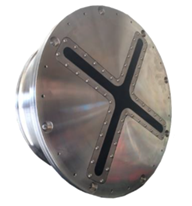
\includegraphics[width=\linewidth]{gfx/chapter-detection/sonar/Sonar_antennas.png}
  \end{minipage}
  \hspace{1cm}
  \begin{minipage}{0.4\linewidth}
    \centering
    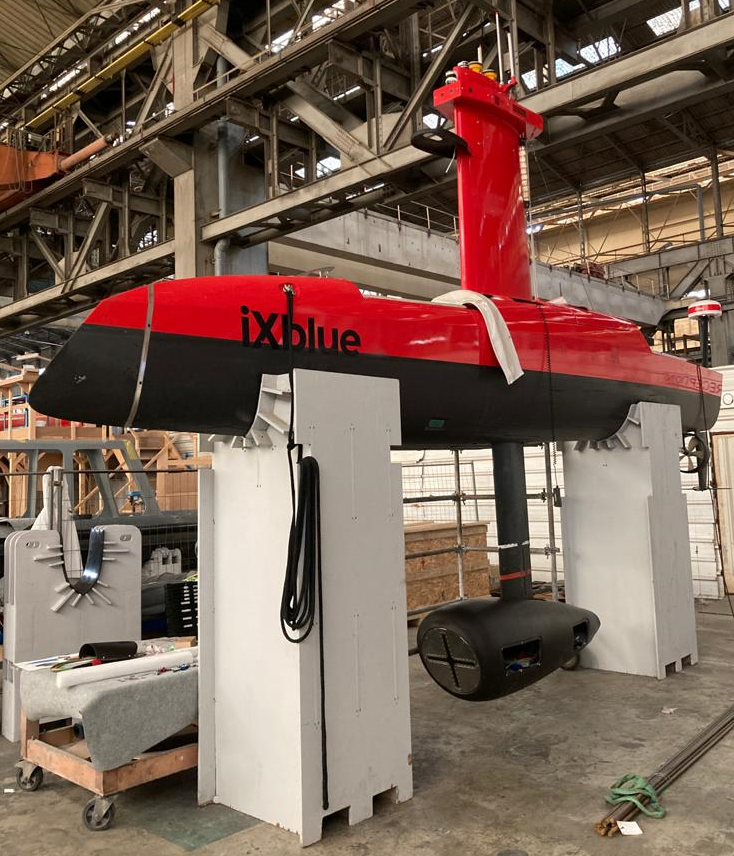
\includegraphics[width=\linewidth]{gfx/chapter-detection/sonar/SPX_and_DriX.png}
  \end{minipage}
  \caption{À gauche: face active du SEAPIX, les deux antennes linéaires de 64 capteurs se croisent en leur centre. À droite: le sonar installé dans la gondole du drone de surface DriX, en configuration de sonar frontal. Figures reprises de \cite{JOE24}.}
  \label{fig:detection-mills-systeme}
\end{figure}

Dans le cadre de la thèse, le SEAPIX est utilisé comme sonar frontal (\emph{forward-looking sonar}, FLS) à bord du drone de surface DriX, la face active orientée vers l'avant et inclinée de $20^\circ$. L'antenne verticale émet un faisceau large de $9^\circ$ en élévation par $120^\circ$ en azimut, puis les deux antennes reçoivent simultanément: l'antenne horizontale forme des voies en azimut et l'antenne verticale des voies en élévation. Les données utilisées ont été acquises en baie de La Ciotat en 2021 et 2022, par 50~m de fond, avec une sphère métallique de 71~cm immergée à 25~m comme cible de référence.

Le problème posé est alors celui de la \cref{def:detection-archetype-cible}: détecter une cible ponctuelle dans la réverbération du milieu. Deux constats sur les données réelles orientent le travail. D'une part, la réverbération n'est pas gaussienne: sur les premières centaines de mètres, la distribution de l'amplitude est proche d'une loi K de paramètre de forme $\nu\simeq3$, et elle ne redevient proche d'une loi normale qu'en fin de portée, là où le bruit ambiant domine \cite{JOE24}. Le modèle msg de la \cref{def:detection-msg} et les détecteurs robustes de la \cref{subsec:detection radar} sont donc le bon point de départ. D'autre part, on dispose de deux antennes qui observent la même scène, et il est naturel de se demander ce que l'on gagne à les traiter conjointement.

\subsection{Modèle de données à deux antennes}
\label{subsec:detection-mills-modele}

Considérons d'abord chaque antenne séparément. Après formation des données en bande de base et compression d'impulsion, l'antenne $\iarray\in\{1,2\}$ fournit à chaque case distance un vecteur $\x_\iarray\in\C^{\Nsensor}$, et une cible ponctuelle vue dans la direction $\doa_\iarray$ s'écrit $\x_\iarray=\amplitude_\iarray\steering_\iarray+\z_\iarray$, avec $\steering_\iarray=\steering(\doa_\iarray)$ le vecteur directionnel de l'antenne. C'est exactement le problème de la \cref{def:detection-archetype-cible}, et l'on peut appliquer sur chaque antenne l'\detname{anmf} construit sur l'estimateur de Tyler \cref{eq:detection-anmf-tyler}. C'est ce qui est fait en pratique sur ce type de système, et c'est la référence à laquelle nous nous comparerons.

Ce traitement antenne par antenne a toutefois un défaut, lié à la corrélation de la réverbération. Chaque antenne présente une zone de moindre détectabilité autour de $0^\circ$ dans sa propre direction, et comme elle ne voit rien de l'autre direction, cette zone s'étend à toute une bande de l'espace: une bande verticale pour l'antenne horizontale, une bande horizontale pour l'antenne verticale. En combinant les deux antennes, une cible n'est aveugle que si elle est mal placée pour les deux à la fois. Pour exploiter cette complémentarité, on concatène les observations:

\begin{definition}[{Modèle à deux antennes}]
\label{def:detection-mills-modele}
  Notons $\x_\iarray\in\C^{\Nsensor}$ le vecteur reçu par l'antenne $\iarray\in\intrange{1}{\Narray}$, avec $\Narray=2$, et
  \begin{equation}
    \x = \begin{bmatrix}\x_1\\\x_2\end{bmatrix}\in\C^{\Narray\Nsensor},
    \qquad
    \Steermat = \begin{bmatrix}\steering_1 & \vector{0}\\\vector{0} & \steering_2\end{bmatrix}\in\C^{\Narray\Nsensor\times\Narray},
    \qquad
    \Vamplitude = \begin{bmatrix}\amplitude_1\\\amplitude_2\end{bmatrix}\in\C^{\Narray}.
    \label{eq:detection-mills-concat}
  \end{equation}
  Le problème de détection prend alors la forme de la \cref{def:detection-archetype-cible} avec $\Steermat\Vamplitude$ pour réponse cible:
  \begin{equation}
    \left\{
    \begin{array}{lll}
      \hypothesis_0: & \x = \z, & \x_\iobs = \z_\iobs, \quad \iobs\in\intrange{1}{\Nobs} \\[2pt]
      \hypothesis_1: & \x = \Steermat\Vamplitude + \z, \qquad & \x_\iobs = \z_\iobs, \quad \iobs\in\intrange{1}{\Nobs}.
    \end{array}
    \right.
    \label{eq:detection-mills-test}
  \end{equation}
\end{definition}

Les amplitudes $\amplitude_1$ et $\amplitude_2$ sont laissées libres, puisque les deux antennes n'ont ni la même ouverture ni le même gain. Reste à décrire le bruit $\z$. Dans la littérature radar, les détecteurs multi-antennes existants supposent soit un fouillis gaussien homogène sur toutes les antennes \sidecite{Chong201004}, soit des antennes non corrélées entre elles \cite{Chong201003}. Aucune de ces deux hypothèses ne convient ici. Les deux antennes n'observent pas la même portion de fond et leurs réverbérations n'ont pas de raison de fluctuer ensemble, mais elles partagent leur capteur central, si bien que les blocs d'intercorrélation ne sont pas nuls. La \cref{fig:detection-mills-covariance} le montre sur une scm estimée sur données réelles. D'où le modèle suivant:

\begin{definition}[{Modèle multi-textures}]
\label{def:detection-mills-multitexture}
  Chaque antenne porte sa propre texture et son propre facteur d'échelle. En posant $\escale_\iarray = \powerscale_\iarray\sqrt{\texture_\iarray}$ et
  \begin{equation}
    \Scalemat = \Diag\left(\escale_1,\escale_2\right)\otimes\Id{\Nsensor},
    \qquad
    \MScatter = \begin{bmatrix}\MScatter_{11} & \MScatter_{12}\\\MScatter_{21} & \MScatter_{22}\end{bmatrix},
    \label{eq:detection-mills-scalemat}
  \end{equation}
  la dispersion de l'observation vaut
  \begin{equation}
    \MCov = \Scalemat\,\MScatter\,\Scalemat,
    \label{eq:detection-mills-cov}
  \end{equation}
  où $\MScatter_{\iarray\iarray}$ est le bloc propre à l'antenne $\iarray$ et $\MScatter_{12}=\MScatter_{21}^\herm$ le bloc d'intercorrélation. Conditionnellement aux textures, les densités sous les deux hypothèses s'écrivent
  \begin{equation}
    \ddp{\x}(\x;\hypothesis_0) = \frac{\exp\left(-\quadraticH{\x}{\MCov}\right)}{\pi^{\Narray\Nsensor}\Det(\MCov)},
    \qquad
    \ddp{\x}(\x;\hypothesis_1) = \frac{\exp\left(-(\x-\Steermat\Vamplitude)^\herm\inv{\MCov}(\x-\Steermat\Vamplitude)\right)}{\pi^{\Narray\Nsensor}\Det(\MCov)}.
    \label{eq:detection-mills-pdf}
  \end{equation}
\end{definition}

\begin{figure}[htbp]
  \centering
  \begin{minipage}{0.45\linewidth}
    \includegraphics[width=\linewidth]{gfx/chapter-detection/sonar/SCM_example.pdf}
  \end{minipage}
  \begin{minipage}{0.45\linewidth}
    \includegraphics[width=\linewidth]{gfx/chapter-detection/sonar/Covariance_model.pdf}
  \end{minipage}
  \caption{À gauche: scm estimée sur données réelles SEAPIX dans une zone homogène entre 265~m et 328~m (en dB). Les blocs diagonaux correspondent à chaque antenne, les blocs hors diagonale à leur intercorrélation, qui n'est pas nulle. À droite: le modèle de covariance utilisé en simulation, $[\MScatter]_{jl}=\beta\rho_1^{\abs{j_1-l_1}}\rho_2^{\abs{j_2-l_2}}$ avec $\beta=3\times10^{-4}$, $\rho_1=0{,}4$ et $\rho_2=0{,}9$. Figures reprises de \cite{JOE24}.}
  \label{fig:detection-mills-covariance}
\end{figure}

\begin{remark}[{Ce que le modèle autorise}]
  Ce modèle permet de décrire deux antennes de statistiques différentes: on peut par exemple avoir une première antenne gaussienne ($\texture_1=1$) et homogène ($\powerscale_1=1$), et une seconde K-distribuée et partiellement homogène. Au sens de la \cref{def:detection-heterogeneite}, il s'agit d'une hétérogénéité \emph{par blocs}, intermédiaire entre le modèle usuel à une seule texture pour tout le vecteur et le cas où chaque capteur aurait la sienne, où plus rien ne serait identifiable. Le bloc $\MScatter_{12}$ est conservé, et c'est lui qui distingue ce modèle d'un traitement antenne par antenne.
\end{remark}

\subsection{Le trvg et l'apparition d'un terme croisé}
\label{subsec:detection-mills-tests}

Suivons la démarche en deux étapes de la \cref{subsec:detection radar}: on suppose d'abord $\MScatter$ connue, on dérive le test, puis on remplace $\MScatter$ par une estimée. À $\MScatter$ connue, les paramètres inconnus sont les amplitudes $\Vamplitude$ et les deux échelles $\escale_1,\escale_2$. Le trvg s'obtient en maximisant la vraisemblance en ces paramètres sous chaque hypothèse, et on obtient le résultat suivant \cite{JOE24}:

\begin{proposition}[{trvg à deux textures}]
\label{prop:detection-mills-glrt}
  Le trvg du problème \cref{eq:detection-mills-test} à $\MScatter$ connue s'écrit comme le quotient des échelles estimées sous chaque hypothèse:
  \begin{equation}
    \statGLRT(\x)
    =
    \frac{\hat{\escale}_{1,0}\,\hat{\escale}_{2,0}}{\hat{\escale}_{1,1}\,\hat{\escale}_{2,1}}
    \detect,
    \label{eq:detection-mills-glrt}
  \end{equation}
  où, en notant $\left[\inv{\MScatter}\right]_{\iarray\ivarbis}$ le bloc $(\iarray,\ivarbis)$ de $\inv{\MScatter}$,
  \begin{equation}
    \left(\hat{\escale}_{1,0}\,\hat{\escale}_{2,0}\right)^2
    =
    \frac{\Realp\left(\x_1^\herm\left[\inv{\MScatter}\right]_{12}\x_2\right)}{\Nsensor}
    +
    \sqrt{
      \frac{\x_1^\herm\left[\inv{\MScatter}\right]_{11}\x_1}{\Nsensor}
      \cdot
      \frac{\x_2^\herm\left[\inv{\MScatter}\right]_{22}\x_2}{\Nsensor}
    },
    \label{eq:detection-mills-sigma0}
  \end{equation}
  et où $\left(\hat{\escale}_{1,1}\,\hat{\escale}_{2,1}\right)^2$ est donnée par la même expression en substituant $\inv{\MScatter}-\projspace{\MScatter}$ à $\inv{\MScatter}$, avec
  \begin{equation}
    \projspace{\MScatter}
    =
    \inv{\MScatter}\Steermat\left(\Steermat^\herm\inv{\MScatter}\Steermat\right)^{-1}\Steermat^\herm\inv{\MScatter}.
    \label{eq:detection-mills-projecteur}
  \end{equation}
\end{proposition}

Le détecteur est donc un rapport des puissances résiduelles estimées sans et avec la cible, comme le \detname{nmf} en mono-antenne. La nouveauté est dans \cref{eq:detection-mills-sigma0}: en plus des deux formes quadratiques propres à chaque antenne apparaît le terme croisé $\Realp(\x_1^\herm[\inv{\MScatter}]_{12}\x_2)$, qui fait intervenir la corrélation entre les deux antennes dans l'estimation de leurs échelles. C'est ce terme qui permet de situer le détecteur par rapport à ceux de la littérature:
\begin{itemize}
  \item pour une seule antenne, \cref{eq:detection-mills-glrt} se ramène, à une transformation monotone près, au \detname{nmf} \cref{eq:detection-nmf};
  \item lorsque les antennes sont décorrélées, $[\inv{\MScatter}]_{12}=\mat{0}$, le terme croisé disparaît et l'on retrouve le détecteur \textsc{mimo} de \citet{Chong201003}, c'est-à-dire un produit de deux \detname{nmf};
  \item lorsque les deux échelles sont égales, on retrouve la version par sous-espace de l'\textsc{ace} \cite{Raghavan2016}.
\end{itemize}
Le trvg à deux textures est donc une généralisation bi-antenne du \detname{nmf}, que l'on notera \detname{m-nmf-g}, et sa version adaptative une généralisation de l'\detname{anmf}.

\begin{property}[{Invariance aux textures}]
\label{prop:detection-mills-cfar}
  La statistique \cref{eq:detection-mills-glrt} est texture-cfar au sens de la \cref{def:detection-cfar}: sa loi sous $\hypothesis_0$ ne dépend ni de $\texture_1$ ni de $\texture_2$.
\end{property}

\subsection{Pourquoi passer au test de Rao}
\label{subsec:detection-mills-rao}

Le trvg \cref{eq:detection-mills-glrt} présente deux inconvénients pratiques. Le premier est son coût: les échelles sous $\hypothesis_1$ font intervenir le projecteur $\projspace{\MScatter}$, qui dépend de la direction testée $(\doa_1,\doa_2)$. Il faut donc les recalculer pour chaque couple de directions, alors que le balayage porte sur $64\times64$ couples par case distance. Le second est sa loi: si l'on dispose d'une relation $\pfa$-seuil exacte à $\MScatter$ connue, les simulations montrent que la version adaptative n'est plus matrice-cfar lorsque la fausse alarme visée est faible \cite{JOE24}, ce qui empêche de fixer un seuil une fois pour toutes.

Le test de Rao répond aux deux. Il ne demande l'estimation des paramètres de nuisance que sous $\hypothesis_0$, et sous $\hypothesis_0$ les échelles estimées \cref{eq:detection-mills-sigma0} ne dépendent pas de $\Steermat$: une seule estimation par case distance sert à tout le balayage angulaire. En écrivant le problème sous la forme \cref{eq:detection-test-parametre} avec $\paramtest=[\Realp(\Vamplitude)^\T,\operatorname{Im}(\Vamplitude)^\T]^\T\in\R^4$ et $\paramnuis=[\escale_1,\escale_2]^\T$, on obtient \sidecite{GRETSI23a}:

\begin{proposition}[{Test de Rao à deux textures}]
\label{prop:detection-mills-rao}
  Le test de Rao du problème \cref{eq:detection-mills-test} s'écrit comme une énergie projetée:
  \begin{equation}
    \statRao(\x)
    =
    2\,\x^\herm\inv{\widehat{\MCov}_0}\Steermat
    \left(\Steermat^\herm\inv{\widehat{\MCov}_0}\Steermat\right)^{-1}
    \Steermat^\herm\inv{\widehat{\MCov}_0}\,\x
    \detect,
    \label{eq:detection-mills-rao}
  \end{equation}
  où $\widehat{\MCov}_0 = \widehat{\Scalemat}_0\,\MScatter\,\widehat{\Scalemat}_0$, les échelles de $\widehat{\Scalemat}_0$ valant
  \begin{equation}
    \hat{\escale}_{1,0}^2 = s_1 + \sqrt{\frac{s_1}{s_2}}\,s_{12},
    \qquad
    \hat{\escale}_{2,0}^2 = s_2 + \sqrt{\frac{s_2}{s_1}}\,s_{12},
    \label{eq:detection-mills-echelles-h0}
  \end{equation}
  avec $s_\iarray = \x_\iarray^\herm[\inv{\MScatter}]_{\iarray\iarray}\x_\iarray/\Nsensor$ et $s_{12}=\Realp(\x_1^\herm[\inv{\MScatter}]_{12}\x_2)/\Nsensor$.
\end{proposition}

On reconnaît dans \cref{eq:detection-mills-rao} le filtre adapté \textsc{mimo} de \sidecite{Chong201004}, qui est le détecteur optimal en fouillis gaussien homogène à covariance connue, évalué ici en une covariance dont les échelles de chaque antenne ont été estimées sur l'observation elle-même. On retrouve aussi le terme croisé $s_{12}$, cette fois dans l'estimation des échelles. Le test est texture-cfar, et sa forme d'énergie projetée donne directement sa loi sous $\hypothesis_0$:

\begin{proposition}[{Relation $\pfa$-seuil du test de Rao}]
\label{prop:detection-mills-rao-pfa}
  Sous $\hypothesis_0$, $\statRao$ suit asymptotiquement (en $\Nsensor$) une loi du $\chisquared$ à quatre degrés de liberté, d'où
  \begin{equation}
    \pfa = \exp\left(-\frac{\DetectorTreshold}{2}\right)\left(1+\frac{\DetectorTreshold}{2}\right),
    \label{eq:detection-mills-rao-pfa}
  \end{equation}
  qui ne dépend ni des textures ni de $\MScatter$.
\end{proposition}

En simulation, le régime asymptotique est atteint dès $\Nsensor=64$, ce qui est le cas du SEAPIX, et la relation \cref{eq:detection-mills-rao-pfa} reste vérifiée en version adaptative pour des matrices de covariance très différentes \cite{JOE24}. C'est la raison principale pour laquelle nous privilégions le test de Rao, que l'on notera \detname{m-nmf-r}.

\begin{remark}[{Pourquoi le test de Rao}]
\label{rem:detection-pourquoi-rao}
  Le test de Rao est souvent présenté comme une approximation du trvg, plus simple à calculer. Ici, il présente trois avantages qui dépassent la simplicité de calcul. D'abord, l'estimée sous $\hypothesis_0$ ne dépend pas de la direction testée, ce qui rend le balayage angulaire peu coûteux. Ensuite, sa loi sous $\hypothesis_0$ est connue en forme close et ne dépend pas de la covariance pour $\Nsensor$ grand, ce qui permet de régler le seuil sans simulation. Enfin, comme il est construit au voisinage de $\hypothesis_0$, il ne cherche pas à expliquer l'observation par un signal quelconque, et il est plus sélectif vis-à-vis des signaux qui ne correspondent pas à la direction testée. Ce dernier point sera mis en regard, en \cref{sec:detection-fls}, du choix inverse que font les détecteurs par sous-espaces.
\end{remark}

\subsection{Estimation robuste sous textures multiples}
\label{subsec:detection-mills-estimation}

Reste la seconde étape: remplacer $\MScatter$ par une estimée issue de $\Nobs$ données secondaires. En fouillis gaussien, la scm convient, mais en fouillis msg elle est dominée par les données de forte puissance. Il faut donc un estimateur de Tyler adapté au modèle à deux textures. En maximisant la vraisemblance des données secondaires sous le modèle de la \cref{def:detection-mills-multitexture}, on obtient \sidecite{JOE24}:

\begin{proposition}[{Estimateur de Tyler à deux textures}]
\label{prop:detection-mills-tyler}
  Sous le modèle de la \cref{def:detection-mills-multitexture}, l'estimateur du maximum de vraisemblance de $\MScatter$ vérifie
  \begin{equation}
    \widehat{\MScatter}
    =
    \frac{1}{\Nobs}\sum_{\iobs=1}^{\Nobs}
    \inv{\widehat{\mat{T}}_\iobs}\,\x_\iobs\x_\iobs^\herm\,\inv{\widehat{\mat{T}}_\iobs},
    \qquad
    \widehat{\mat{T}}_\iobs = \Diag\left(\sqrt{\hat{\texture}_{1,\iobs}},\sqrt{\hat{\texture}_{2,\iobs}}\right)\otimes\Id{\Nsensor},
    \label{eq:detection-mills-tyler}
  \end{equation}
  où les textures $\hat{\texture}_{1,\iobs}$ et $\hat{\texture}_{2,\iobs}$ sont données par \cref{eq:detection-mills-echelles-h0} appliquée à $\x_\iobs$ et à $\widehat{\MScatter}$.
\end{proposition}

On retrouve la structure de l'estimateur de Tyler (\cref{def:context-complex-tyler}): chaque donnée est normalisée par sa propre puissance avant d'être moyennée, ce qui rend l'estimée indépendante des textures. La différence est que la normalisation se fait par bloc, et que la texture d'une antenne est estimée en tenant compte, à travers le terme croisé, de ce qu'observe l'autre. L'estimateur se calcule par un algorithme de point fixe, dont la convergence est rapide en pratique\footnote{L'existence et l'unicité de la solution ne sont en revanche pas établies. Voir l'annexe~D de l'article reproduit p.~\paperpage{JOE24} pour la dérivation et l'algorithme.}. En remplaçant $\MScatter$ par $\widehat{\MScatter}$ dans \cref{eq:detection-mills-glrt,eq:detection-mills-rao}, on obtient les versions adaptatives des deux détecteurs.

\subsection{Ce que la fusion des antennes apporte}
\label{subsec:detection-mills-perf}

Les simulations de \cite{JOE24} utilisent le modèle de covariance de la \cref{fig:detection-mills-covariance}, $\Nobs=2\times2\Nsensor=256$ données secondaires et $\pfa=10^{-2}$. On peut en retenir les éléments suivants:
\begin{itemize}
  \item à covariance connue, en fouillis gaussien, les détecteurs bi-antennes gagnent environ 2,5~dB et 2~dB par rapport aux \detname{nmf} de chacune des antennes, à $\pdet=0{,}8$, et ne sont qu'à 0,2~dB du filtre adapté \textsc{mimo} qui connaît toute la covariance;
  \item le gain se lit surtout dans le plan azimut-élévation: là où l'antenne horizontale seule a une probabilité de détection de 0,17 sur toute la bande $\doa_1=0^\circ$, et l'antenne verticale 0,03 sur la bande $\doa_2=0^\circ$, le test de Rao dépasse 0,8 dès que $\abs{\doa_2}>10{,}5^\circ$. La zone aveugle se réduit à un voisinage du centre;
  \item en fouillis gaussien partiellement homogène, le filtre adapté \textsc{mimo} adaptatif ne contrôle plus la fausse alarme et devient moins bon que l'\detname{anmf} mono-antenne, alors que les détecteurs proposés ne sont pas affectés, étant invariants aux échelles;
  \item en fouillis K-distribué ($\nu=0{,}5$), l'estimateur à deux textures apporte environ 1,2~dB par rapport à la scm, et 3~dB par rapport au meilleur des détecteurs concurrents.
\end{itemize}

% ============================== FIGURE 4/9 =========================================
% ATTENTION: RUN DEBUG (n_h0 = n_h1 = 200, 12 points de rsb au lieu de 150).
% Version definitive:
%   uv run qanat experiment run sonar_pd_snr --n-trials-h0 10000 --n-trials-h1 10000
% puis --k-dist pour le second panneau. La provenance porte debug=True tant que
% ce n'est pas fait.
%
% TODO: cette figure n'a pour l'instant que le cas gaussien. Le plan en demande
% deux, gaussien et K-distribue (nu = 0.5), cote a cote --- c'est la comparaison
% qui porte l'argument (la robustesse coute peu sous modele gaussien et rapporte
% beaucoup sinon). Relancer avec --k-dist et enregistrer sous l'id pd-rsb-k.
%
% TODO decision: le MATLAB de reference trace chaque famille de courbes sur SON
% propre axe de rsb (snrP pour l'antenne 1, snrA pour l'antenne 2, snrPA pour le
% bi-antenne), ce que l'article ne dit nulle part. Ici tout est sur un axe
% commun, d'ou l'ecart mono-antenne 1 / mono-antenne 2 plus marque que dans
% l'article. A trancher: axe commun (honnete mais different de l'article) ou
% convention de l'article (comparable mais a expliquer en note).
% ====================================================================================
\begin{figure}[htbp]
  \centering
  % This file was created with matplot2tikz v0.5.3.
\begin{tikzpicture}

\definecolor{cornflowerblue92168211}{RGB}{92,168,211}
\definecolor{darkgray176}{RGB}{176,176,176}
\definecolor{indianred224107107}{RGB}{224,107,107}
\definecolor{mediumpurple165123197}{RGB}{165,123,197}
\definecolor{mediumseagreen107191107}{RGB}{107,191,107}
\definecolor{mediumturquoise80200192}{RGB}{80,200,192}
\definecolor{sandybrown22416080}{RGB}{224,160,80}

\begin{axis}[
height=5cm,
label style={font=\footnotesize},
legend cell align={left},
legend style={
  fill opacity=0.8,
  draw opacity=1,
  text opacity=1,
  at={(1.02,1)},
  anchor=north west,
  draw=none
},
legend style={draw=none, fill=white, fill opacity=0.9, text opacity=1, font=\footnotesize},
tick align=outside,
tick label style={font=\scriptsize},
tick pos=left,
title style={font=\footnotesize, yshift=-2pt},
width=\textwidth,
x grid style={darkgray176},
xlabel={SNR (dB)},
xmin=-26.5, xmax=6.5,
xtick style={color=black},
y grid style={darkgray176},
ylabel={PD},
ymin=-0.02, ymax=1.02,
ytick style={color=black}
]
\addplot [semithick, cornflowerblue92168211]
table {%
-25 0.015
-22.2727272727273 0.025
-19.5454545454545 0.055
-16.8181818181818 0.135
-14.0909090909091 0.39
-11.3636363636364 0.84
-8.63636363636364 1
-5.90909090909091 1
-3.18181818181818 1
-0.454545454545457 1
2.27272727272727 1
5 1
};
\addlegendentry{M-NMF-G}
\addplot [semithick, indianred224107107, dashed]
table {%
-25 0.015
-22.2727272727273 0.025
-19.5454545454545 0.055
-16.8181818181818 0.15
-14.0909090909091 0.41
-11.3636363636364 0.845
-8.63636363636364 1
-5.90909090909091 1
-3.18181818181818 1
-0.454545454545457 1
2.27272727272727 1
5 1
};
\addlegendentry{M-NMF-R}
\addplot [semithick, mediumpurple165123197, dash pattern=on 1pt off 3pt on 3pt off 3pt]
table {%
-25 0.02
-22.2727272727273 0.035
-19.5454545454545 0.055
-16.8181818181818 0.16
-14.0909090909091 0.415
-11.3636363636364 0.865
-8.63636363636364 1
-5.90909090909091 1
-3.18181818181818 1
-0.454545454545457 1
2.27272727272727 1
5 1
};
\addlegendentry{M-NMF-I}
\addplot [semithick, mediumseagreen107191107, dotted]
table {%
-25 0.015
-22.2727272727273 0.025
-19.5454545454545 0.02
-16.8181818181818 0.04
-14.0909090909091 0.065
-11.3636363636364 0.135
-8.63636363636364 0.32
-5.90909090909091 0.525
-3.18181818181818 0.84
-0.454545454545457 0.995
2.27272727272727 1
5 1
};
\addlegendentry{SA-1}
\addplot [semithick, sandybrown22416080, dash pattern=on 3pt off 1pt on 1pt off 1pt]
table {%
-25 0.02
-22.2727272727273 0.05
-19.5454545454545 0.06
-16.8181818181818 0.185
-14.0909090909091 0.435
-11.3636363636364 0.84
-8.63636363636364 0.995
-5.90909090909091 1
-3.18181818181818 1
-0.454545454545457 1
2.27272727272727 1
5 1
};
\addlegendentry{SA-2}
\addplot [semithick, mediumturquoise80200192, dash pattern=on 5pt off 2pt]
table {%
-25 0.025
-22.2727272727273 0.065
-19.5454545454545 0.085
-16.8181818181818 0.225
-14.0909090909091 0.53
-11.3636363636364 0.905
-8.63636363636364 1
-5.90909090909091 1
-3.18181818181818 1
-0.454545454545457 1
2.27272727272727 1
5 1
};
\addlegendentry{MIMO-MF}
\addplot [semithick, cornflowerblue92168211]
table {%
-25 0
-22.2727272727273 0.01
-19.5454545454545 0.015
-16.8181818181818 0.035
-14.0909090909091 0.07
-11.3636363636364 0.33
-8.63636363636364 0.75
-5.90909090909091 0.955
-3.18181818181818 1
-0.454545454545457 1
2.27272727272727 1
5 1
};
\addlegendentry{M-ANMF-G-TYL}
\addplot [semithick, indianred224107107, dashed]
table {%
-25 0
-22.2727272727273 0.01
-19.5454545454545 0.015
-16.8181818181818 0.035
-14.0909090909091 0.07
-11.3636363636364 0.31
-8.63636363636364 0.73
-5.90909090909091 0.95
-3.18181818181818 1
-0.454545454545457 1
2.27272727272727 1
5 1
};
\addlegendentry{M-ANMF-R-TYL}
\addplot [semithick, mediumpurple165123197, dash pattern=on 1pt off 3pt on 3pt off 3pt]
table {%
-25 0.015
-22.2727272727273 0.02
-19.5454545454545 0.02
-16.8181818181818 0.035
-14.0909090909091 0.135
-11.3636363636364 0.39
-8.63636363636364 0.745
-5.90909090909091 1
-3.18181818181818 1
-0.454545454545457 1
2.27272727272727 1
5 1
};
\addlegendentry{M-ANMF-G-SCM}
\addplot [semithick, mediumseagreen107191107, dotted]
table {%
-25 0.015
-22.2727272727273 0.02
-19.5454545454545 0.02
-16.8181818181818 0.035
-14.0909090909091 0.135
-11.3636363636364 0.355
-8.63636363636364 0.75
-5.90909090909091 1
-3.18181818181818 1
-0.454545454545457 1
2.27272727272727 1
5 1
};
\addlegendentry{M-ANMF-R-SCM}
\end{axis}

\end{tikzpicture}

  \provPdRsbQR[1cm]
  \caption{$\pdet$ en fonction du rapport signal à bruit, à $\pfa=10^{-2}$, en
  fouillis gaussien ($m=64$, $\Nobs=256$, pointage $\theta_1=\theta_2=45^\circ$).
  Le filtre adapte mimo à dispersion connue borne les performances; les tests
  glrt et de Rao à dispersion connue s'en approchent à quelques dixiemes de dB,
  et leurs versions adaptatives paient l'estimation. Les detecteurs
  mono-antenne restent en retrait: c'est le gain de la fusion des deux
  antennes. \provPdRsb}
  \label{fig:detection-mills-pd-rsb}
\end{figure}

\wipfig{FIGURE 3/9}{Carte $\pdet(\doa_1,\doa_2)$ pour \detname{nmf} 1, \detname{nmf} 2 et le test de Rao à covariance connue, RSB $=-12$~dB. Expérience: sonar\_pd\_angle.}

Sur données réelles, la cible de référence est correctement localisée en azimut et en élévation par les deux détecteurs. L'intérêt de l'estimateur robuste apparaît lorsque les données secondaires sont contaminées: en ajoutant une cible synthétique à 100 cases distance de la cible réelle, le test de Rao construit sur la scm ne permet plus de distinguer la cible et place son maximum au mauvais endroit, alors que la version construite sur l'estimateur à deux textures reste exploitable (\cref{fig:detection-mills-contamination}).

\begin{figure}[htbp]
  \centering
  \includegraphics[width=0.49\linewidth]{gfx/chapter-detection/sonar/M_ANMF_R_SCM_corrupted_output.pdf}
  \includegraphics[width=0.49\linewidth]{gfx/chapter-detection/sonar/M_ANMF_R_TYL_corrupted_output.pdf}
  \caption{Sortie du test de Rao adaptatif sur données réelles SEAPIX lorsque les données secondaires sont contaminées par une seconde cible. À gauche avec la scm, à droite avec l'estimateur à deux textures \cref{eq:detection-mills-tyler}, tous deux sur 256 données secondaires. Figures reprises de \cite{JOE24}, les données n'étant pas diffusables.}
  \label{fig:detection-mills-contamination}
\end{figure}

\section{Détection multi-pings et sous-espaces pour un sonar frontal}
\label{sec:detection-fls}

\begin{contributions}
  Cette section reprend \fullcite{JOE26}.
\end{contributions}

% ============================ TODO texte (~2 paragraphes) ==========================
% Transition depuis la section precedente, puis contexte:
%  - on y exploitait une structure *entre antennes*; on exploite ici une
%    structure *entre pings* successifs, c'est-a-dire une integration coherente
%    dans le temps --- l'analogue sonar du traitement espace-temps (stap) du
%    radar;
%  - le gain attendu: sommer en phase $\Nping$ echos ameliore le rapport signal
%    a bruit; le prix a payer: la dimension du probleme est multipliee par
%    $\Nping$, et le nombre de donnees secondaires necessaires avec elle. C'est
%    exactement le probleme annonce en fin de \cref{sec:detection-cadre};
%  - second prix a payer, moins evident et c'est le fil de la section: sommer
%    en phase suppose de connaitre la phase. Toute erreur de recalage degrade
%    la detection, d'ou la seconde moitie de la section sur les sous-espaces.
% ====================================================================================

\subsection{Modèle multi-pings}
\label{subsec:detection-fls-modele}

\begin{definition}[{Modèle multi-pings}]
\label{def:detection-fls-modele}
  Après recalage, la concaténation des $\Nping$ pings s'écrit $\x = [\x_1^\T\ \cdots\ \x_{\Nping}^\T]^\T\in\C^{\Nsensor\Nping}$ et la réponse d'une cible ponctuelle vue dans la direction $\doa$ vaut
  \begin{equation}
    \x = \amplitude\,\steerfull(\doa) + \z,
    \qquad
    \steerfull(\doa) = \vector{1}_{\Nping}\otimes\steering(\doa),
    \label{eq:detection-fls-modele}
  \end{equation}
  où $\vector{1}_{\Nping}\in\R^{\Nping}$ est le vecteur de composantes unité et $\steering(\doa)\in\C^{\Nsensor}$ le vecteur directionnel d'un ping.
\end{definition}

% ======================= TODO texte (remarque, ~5 lignes) ==========================
% Lire la decomposition de Kronecker de \cref{eq:detection-fls-modele}, elle
% structure toute la section: l'operande de gauche est *interferometrique* (il
% somme en phase les echos ping a ping), celui de droite est purement
% *angulaire* (il somme en phase les capteurs dans la direction $\doa$). Le
% vecteur $\vector{1}_{\Nping}$ suppose un recalage parfait --- hypothese que
% la \cref{subsec:detection-fls-sousespace} viendra relacher, et c'est
% precisement sur cet operande de gauche que portera le sous-espace.
% Renvoyer au pdf joint pour la chaine de recalage elle-meme, qui n'est pas
% reprise ici.
% ====================================================================================

\subsection{Structure de Kronecker de la dispersion du fouillis}
\label{subsec:detection-fls-kronecker}

\begin{proposition}[{Structure de la dispersion du fouillis}]
\label{prop:detection-fls-kronecker}
  En modélisant le fouillis comme la somme des contributions indépendantes de $N_c$ facettes insonifiées, de réponses $\z_n = \amplitude_n\,\vector{1}_{\Nping}\otimes\steering(\doa_n)$ avec $\E\{\amplitude_\ivar\conj{\amplitude_\ivarbis}\}=0$ pour $\ivar\neq\ivarbis$, la dispersion du fouillis vaut
  \begin{equation}
    \MScatter_c
    =
    \sum_{n=1}^{N_c}\E\left\{\abs{\amplitude_n}^2\right\}\,
    \vector{1}_{\Nping}\vector{1}_{\Nping}^\herm
    \otimes
    \steering(\doa_n)\steering(\doa_n)^\herm.
    \label{eq:detection-fls-kronecker}
  \end{equation}
  Elle possède donc naturellement une structure de produit de Kronecker.
\end{proposition}

% ======================= TODO texte (remarque, ~5 lignes) ==========================
% Souligner que la structure est *derivee* et non postulee: elle decoule du
% modele physique de reverberation, alors que la litterature l'introduit le
% plus souvent comme une hypothese de commodite \sidecite{Wirfalt2014}.
% Ajouter que l'operande angulaire herite en outre d'une structure Toeplitz du
% fait de l'antenne lineaire uniforme, et qu'une ponderation des fluctuations
% de reflectivite ping a ping (intrinsic clutter motion, \sidecite{Lombardo2001})
% ne remet pas en cause la forme \cref{eq:detection-fls-kronecker}.
% ====================================================================================

\begin{proposition}[{Nombre de paramètres}]
\label{prop:detection-fls-comptage}
  Une dispersion hermitienne non structurée de taille $\Nsensor\Nping$ compte $(\Nsensor\Nping)^2$ paramètres réels. Sous la contrainte $\MScatter=\Kronleft\otimes\Kronright$ avec $\Kronleft\in\HPD{\Nping}$ et $\Kronright\in\HPD{\Nsensor}$ Toeplitz, ce nombre tombe à
  \begin{equation}
    \Nping^2 + 2\Nsensor - 1 - 1,
    \label{eq:detection-fls-comptage}
  \end{equation}
  le dernier terme retranchant l'indétermination d'échelle entre les deux opérandes.
\end{proposition}

% ======================= TODO texte (~4 lignes) --- CHIFFRE CLE ====================
% Faire l'application numerique, c'est l'argument qui justifie toute la
% section et il n'apparait pas dans l'article: pour $\Nsensor=64$ et
% $\Nping=5$, on passe de $102\,400$ a $151$ parametres reels, soit un facteur
% $\simeq 680$. Rapprocher ce chiffre de la regle $\Nobs\simeq2\vdim$ evoquee
% en \cref{sec:detection-cadre}: sans structure, il faudrait $\Nobs=640$
% donnees secondaires, soit environ 44 m de fond suppose homogene --- une
% hypothese que la scene ne verifie pas. C'est la que se joue le passage du
% principe a l'operationnel.
% ====================================================================================

\subsection{Estimation robuste structurée}
\label{subsec:detection-fls-estimation}

\begin{definition}[{Problème d'estimation structurée}]
\label{def:detection-fls-optim}
  En notant $\obsmat_\iobs$ la matrice telle que $\vecop(\obsmat_\iobs)=\x_\iobs$, l'estimation robuste sous contrainte de structure s'écrit \sidecite[-1cm]{sun2016robust}
  \begin{equation}
    \begin{array}{ll}
      \displaystyle\min_{\Kronleft,\,\Kronright\succ\vector{0}} & \loss\left(\Kronleft,\Kronright\right) \\[4pt]
      \text{sous contrainte} & \Kronright \in \Toep{\Nsensor}
    \end{array}
    \label{eq:detection-fls-optim}
  \end{equation}
  avec le critère de type Tyler
  \begin{equation}
    \loss\left(\Kronleft,\Kronright\right)
    =
    \Nsensor\ln\Det(\Kronleft)
    + \Nping\ln\Det(\Kronright)
    + \frac{\Nsensor\Nping}{\Nobs}\sum_{\iobs=1}^{\Nobs}
      \ln\trace{\Kronleft^{-\T}\obsmat_\iobs^\herm\inv{\Kronright}\obsmat_\iobs}.
    \label{eq:detection-fls-cout}
  \end{equation}
\end{definition}

% ======================= TODO texte (~3 lignes) ====================================
% Signaler la seule difference avec \sidecite{sun2016robust}: la transposee de
% $\inv{\Kronleft}$ dans la trace, qui est ce qui permet de traiter un operande
% $\Kronleft$ *complexe* et non reel. C'est un ajout modeste mais necessaire
% ici, l'operande interferometrique etant complexe par nature.
% ====================================================================================

\begin{proposition}[{Point fixe sur l'opérande interférométrique}]
\label{prop:detection-fls-A}
  À $\Kronright$ fixée, le minimiseur de \cref{eq:detection-fls-cout} sous la normalisation $\trace{\Kronleft}=1$ vérifie
  \begin{equation}
    \widehat{\Kronleft}
    =
    \frac{\Nping}{\Nobs}\sum_{\iobs=1}^{\Nobs}
    \frac{\left(\obsmat_\iobs^\herm\inv{\Kronright}\obsmat_\iobs\right)^\T}
         {\trace{\widehat{\Kronleft}^{-\T}\obsmat_\iobs^\herm\inv{\Kronright}\obsmat_\iobs}}.
    \label{eq:detection-fls-A}
  \end{equation}
\end{proposition}

\begin{proposition}[{Opérande angulaire Toeplitz}]
\label{prop:detection-fls-B}
  À $\Kronleft$ fixée, la contrainte Toeplitz se traite par plongement circulant: on écrit $\Kronright = \Unit\eigset\Unit^\herm$ avec $\Unit = \left[\Id{\Nsensor}\ \vector{0}_{\Nsensor,\Nsensor-1}\right]\mat{F}_{2\Nsensor-1}$, où $\mat{F}_{2\Nsensor-1}$ est la matrice de Fourier normalisée, de sorte que l'estimation de $\Kronright$ se ramène à celle des éléments diagonaux de $\eigset$, obtenus par l'itération de majoration-minimisation de l'\cref{alg:detection-fls-bcd}.
\end{proposition}

\begin{algorithm}[h]
\caption{Estimation robuste à structure Kronecker et Toeplitz}
\label{alg:detection-fls-bcd}
\begin{algorithmic}[1]
  \Require $\{\x_\iobs\}_{\iobs=1}^{\Nobs}$, $\Kronleft^{(0)}=\Id{\Nping}/\Nping$, $\eigset^{(0)}=\Id{2\Nsensor-1}$
  \While{convergence non atteinte}
    \State mettre à jour $\Kronleft$ par itération de \cref{eq:detection-fls-A} à $\Kronright$ fixée, puis normaliser par $\trace{\Kronleft}$
    \State $\vector{w} \gets \Diag\left(\Unit^\herm\inv{\Kronright}\Unit\right)$
    \State $\obsmat \gets \dfrac{\Nsensor}{\Nobs}\displaystyle\sum_{\iobs=1}^{\Nobs}\dfrac{\obsmat_\iobs\Kronleft^{-\T}\obsmat_\iobs^\herm}{\trace{\Kronleft^{-\T}\obsmat_\iobs^\herm\inv{\Kronright}\obsmat_\iobs}}$
    \State $\vector{d} \gets \Diag\left(\eigset\Unit^\herm\inv{\Kronright}\obsmat\inv{\Kronright}\Unit\eigset\right)$
    \State $\left[\vector{\eig}\right]_\ivar \gets \sqrt{\left[\vector{d}\right]_\ivar/\left[\vector{w}\right]_\ivar}$, \quad $\ivar\in\intrange{1}{2\Nsensor-1}$
    \State $\Kronright \gets \Unit\Diag\left(\vector{\eig}\right)\Unit^\herm$, puis normaliser par $\trace{\Kronright}$
  \EndWhile
  \Ensure $\widehat{\MScatter} = \Kronleft\otimes\Kronright$
\end{algorithmic}
\end{algorithm}

% ======================= TODO texte (remarque, ~6 lignes) ==========================
% Deux remarques a ecrire ici:
%  1. cas de l'antenne a element manquant: les deux antennes de la croix se
%     croisent en un capteur central qui ne peut appartenir aux deux, si bien
%     que l'antenne verticale est une ULA de 65 elements dont le central
%     manque. Le raisonnement reste valable a une matrice de permutation pres,
%     en modifiant $\Unit$ en consequence --- indispensable en pratique, faute
%     de quoi les resultats se degradent nettement. Le detail va dans le pdf
%     joint, une remarque suffit ici;
%  2. lien avec la partie 2, en pointeur et non en detour: le point fixe
%     \cref{eq:detection-fls-A} est une descente de gradient riemannienne sur
%     le cone (\cref{sec:context-riemann-optimization}), et c'est justement la
%     contrainte Toeplitz --- qui ne definit pas une sous-variete du cone
%     stable par l'exponentielle --- qui interdit d'y rester et impose le
%     detour par la majoration-minimisation.
% ====================================================================================

\subsection{Robustesse au désalignement: détection par sous-espace}
\label{subsec:detection-fls-sousespace}

\begin{definition}[{Sous-espace interférométrique}]
\label{def:detection-fls-sousespace}
  Soit $\Steerspace_{\Nrank}\in\C^{\Nsensor\Nping\times\Nrank}$, $\Nrank<\Nsensor\Nping$, de colonnes linéairement indépendantes, de la forme
  \begin{equation}
    \Steerspace_{\Nrank}
    =
    \mat{E}_{\Nrank}\otimes\steering(\doa),
    \qquad
    \left[\mat{E}_{\Nrank}\right]_{\iping\ivar}
    =
    \exp\left(-\frac{4\mathrm{j}\pi\,\xi_{\ivar,\iping}}{\wavelength}\right),
    \label{eq:detection-fls-sousespace}
  \end{equation}
  où les $\xi_{\ivar,\iping}$ sont des décalages de phase ping à ping. Le signal recherché est supposé appartenir au sous-espace engendré par les colonnes de $\Steerspace_{\Nrank}$, de coordonnées inconnues.
\end{definition}

\begin{proposition}[{Détecteur par sous-espace}]
\label{prop:detection-fls-anmf-sousespace}
  Le détecteur exploitant conjointement la structure de la dispersion et celle de la réponse cible s'écrit \sidecite[-1cm]{Kraut2001,Raghavan2016}
  \begin{equation}
    \DetectorStat_{\Nrank}(\x,\doa)
    =
    \frac{\abs{\hat{\steerfull}_{\Nrank}^\herm\inv{\widehat{\MScatter}}\x}^2}
         {\left(\hat{\steerfull}_{\Nrank}^\herm\inv{\widehat{\MScatter}}\hat{\steerfull}_{\Nrank}\right)
          \left(\x^\herm\inv{\widehat{\MScatter}}\x\right)}
    \detect,
    \label{eq:detection-fls-anmf-sousespace}
  \end{equation}
  où le signal estimé est la projection oblique de l'observation sur le sous-espace, dans la métrique induite par $\inv{\widehat{\MScatter}}$:
  \begin{equation}
    \hat{\steerfull}_{\Nrank}
    =
    \Steerspace_{\Nrank}
    \left(\Steerspace_{\Nrank}^\herm\inv{\widehat{\MScatter}}\Steerspace_{\Nrank}\right)^{-1}
    \Steerspace_{\Nrank}^\herm\inv{\widehat{\MScatter}}\,\x.
    \label{eq:detection-fls-projection}
  \end{equation}
\end{proposition}

% ================= TODO texte (remarque, ~8 lignes) --- POINT CLE ==================
% C'est le lien le plus fort entre les deux sections sonar, a ne pas manquer:
%  - la premiere colonne de $\mat{E}_{\Nrank}$ vaut $\vector{1}_{\Nping}$: on
%    retrouve exactement le modele \cref{eq:detection-fls-modele} d'une cible
%    parfaitement alignee en phase, et les colonnes suivantes ajoutent des
%    dephasages residuels;
%  - meme si le dephasage reel n'appartient pas exactement au sous-espace,
%    projeter sur $\Steerspace_{\Nrank}$ reduit l'angle de desadaptation par
%    rapport au cas $\Nrank=1$, d'ou le gain de robustesse;
%  - le rang $\Nrank$ est donc le curseur explicite de l'axe annonce en
%    \cref{rem:detection-pourquoi-rao}: chaque degre de liberte gagne en
%    robustesse au desalignement se paie par une perte sur cible parfaitement
%    alignee, puisque le detecteur accepte davantage de signaux;
%  - conclure que les deux sections sonar instrumentent ainsi le meme axe par
%    deux moyens opposes: le test de Rao en le parcourant vers le pole selectif,
%    le sous-espace en le parcourant vers le pole robuste.
% ====================================================================================

\subsection{Ce que la structure achète}
\label{subsec:detection-fls-perf}
% TODO decision: titre de sous-section a valider (cf. remarque analogue en
% \cref{subsec:detection-mills-perf}).

% ============================ TODO texte + figures =================================
\wipfig{FIGURE 7/9}{Pd vs RSB à N=32 et N=640, avec et sans Kronecker+Toeplitz. RIEN N'EXISTE côté qanat pour le volet FLS multi-pings. Traduit en performance le comptage 102 400 -> 151 paramètres pour m=64, P=5.}

% FIGURE 7/9 --- reproductible, A ECRIRE (rien n'existe cote qanat pour ce volet)
% $\pdet$ vs rapport signal a bruit a $\Nobs=32$ et $\Nobs=640$, avec et sans la
% structure Kronecker+Toeplitz. C'est la traduction en performance du comptage
% de la \cref{prop:detection-fls-comptage}: a $\Nobs=32$, le detecteur non
% structure est inutilisable et le detecteur structure fonctionne. Toute la
% section tient dans cette comparaison.
%
\wipfig{FIGURE 8/9}{Pd vs désadaptation de phase pour r dans {1,3,5}. RIEN N'EXISTE. CONTRAINTE FORTE: cette figure, la 7/9 et la 3/9 doivent partager axes, unités et Pfa --- c'est ce qui transforme l'axe sélectivité/robustesse d'une affirmation en une mesure.}

% FIGURE 8/9 --- reproductible, A ECRIRE
% $\pdet$ vs desadaptation de phase pour $\Nrank\in\{1,3,5\}$. Pendant exact de
% la figure angulaire de \cref{subsec:detection-mills-perf}: memes axes, memes
% unites, meme $\pfa$. Les deux figures lues ensemble donnent l'axe
% selectivite/robustesse en entier, du pole selectif (Rao) au pole robuste
% (sous-espace de rang eleve).
%
% Donnees reelles: sorties reprises de l'article \cite{JOE26}, non
% reproductibles (donnees non distribuables).
% ====================================================================================
\section{Détection de changements en-ligne pour les séries temporelles d'images RSO}
\label{sec:detection-online-change-detection}

\begin{contributions}
  Cette section reprend \fullcite{SP24}. Elle partage avec \fullcite{EUSIPCO21} la géométrie de la structure de Kronecker et le schéma d'estimation récursive, mais pas le modèle: les données y suivent une loi de Student, d'où un gradient et une borne différents.
\end{contributions}

La section précédente a montré qu'une structure de la matrice de covariance permet de réduire le nombre d'échantillons nécessaires à son estimation. Un problème commun à tous les détecteurs robustes vus jusqu'ici reste cependant entier: l'estimation passe par la résolution d'une équation de point fixe, dont le coût devient vite limitant lorsque l'on souhaite améliorer une estimation précédente en y ajoutant de nouvelles données. C'est précisément la situation de la détection de changements sur une série temporelle d'images RSO, où chaque nouvelle acquisition oblige à recalculer l'estimée sous $\hypothesis_0$ sur l'ensemble des dates. Dans ce contexte, la géométrie riemannienne permet de considérer un cadre d'estimation en ligne basé sur un algorithme de descente de gradient stochastique \cite{Zhou_2019}, pour lequel une seule itération suffit à chaque nouvelle image\sideref{sec:context-riemann-optimization}{Optimisation riemannienne}.

Ces travaux ont été menés avec Guillaume Ginolhac, Florent Bouchard et Arnaud Breloy. Ils combinent deux idées: supposer une structure de Kronecker pour la matrice de covariance, qui découle naturellement de la décomposition en ondelettes de \cite{Mian_wavelet_2019} appliquée aux canaux de polarisation, et mettre à jour récursivement l'estimée sous $\hypothesis_0$ par une descente de gradient naturel sur la variété des paramètres. Nous commençons par rappeler le problème et ses limitations pratiques, avant de détailler ces deux contributions puis de les illustrer sur données simulées et réelles.


\subsection{Problématique de la détection de changements sur matrices de covariances}

Commençons d'abord par introduire la problématique et les limitations pratiques des solutions proposées.

Nous considérons le traitement d'une série temporelle d'images RSO multivariée telle que présentée en Figure \ref{fig:example_its}. Dans ce contexte, chaque pixel correspond à un vecteur $\x\in\C^\vdim$, où $\vdim$ correspond usuellement à une diversité polarimétrique ($\vdim=3$ ou $\vdim=4$ selon les modalités) ou bien spectrale ou encore fréquentielle\footnote{\`A noter que dans la plupart des cas, on n'observe jamais une scène avec un capteur ayant une telle diversité mais avec une image de résolution suffisante, il est possible de constuire des images plus basses résolution ayant cette diversité \cite{Mian_wavelet_2019}.}.

\begin{figure*}
    \begin{tikzpicture}[scale=1]

% -------------------------------------------------
% parameters
% -------------------------------------------------
\pgfmathsetmacro{\cubex}{3}
\pgfmathsetmacro{\cubey}{2}
\pgfmathsetmacro{\cubez}{1}
\pgfmathsetmacro{\wf}{0.45}

% window size
\pgfmathsetmacro{\wx}{\wf*\cubex}
\pgfmathsetmacro{\wy}{\wf*\cubey}

% -------------------------------------------------
% cube drawing macro
% #1 = label index (1 or T)
% -------------------------------------------------
\newcommand{\DrawCube}[1]{

% ---- cube ----
\draw [every edge/.append style={densely dashed, opacity=.5}]
  (0,0,0) coordinate (o) -- ++(-\cubex,0,0) coordinate (a)
  -- ++(0,-\cubey,0) coordinate (b)
  edge coordinate[pos=1] (g) ++(0,0,-\cubez)
  -- ++(\cubex,0,0) coordinate (c) -- cycle
  (o) -- ++(0,0,-\cubez) coordinate (d)
  -- ++(0,-\cubey,0) coordinate (e)
  edge (g) -- (c) -- cycle
  (o) -- (a) -- ++(0,0,-\cubez) coordinate (f)
  edge (g) -- (d) -- cycle;

% ---- face center ----
\coordinate (Fc) at (-0.5*\cubex,-0.5*\cubey,0);

% window corners (robust)
\coordinate (W1) at ($(Fc)+(-\wx/2,\wy/2,0)$);
\coordinate (W2) at ($(Fc)+(\wx/2,-\wy/2,0)$);

% filled window
\fill[gray!20] (W1) rectangle (W2);

% 3x3 grid
% --- outer border ---
\draw (W1) rectangle (W2);

% --- vertical grid lines ---
\foreach \i in {1,2}{
  \draw ($(W1)+(\i*\wx/3,0,0)$) --
        ($(W1)+(\i*\wx/3,-\wy,0)$);
}

% --- horizontal grid lines ---
\foreach \i in {1,2}{
  \draw ($(W1)+(0,-\i*\wy/3,0)$) --
        ($(W1)+(\wx,-\i*\wy/3,0)$);
}


% annotation
\node[above=11pt] at (Fc) {$ \mathcal{X}_{\iobs #1}=\x_{\iobs #1}$};

% time label
\node at (-4,-1,0) {$t=#1$};

}

% -------------------------------------------------
% DRAW BOTH CUBES (HORIZONTAL)
% -------------------------------------------------

\foreach \label/\xshift in {1/0, T/7}{
  \begin{scope}[xshift=\xshift cm]
    \DrawCube{\label}
  \end{scope}
}

% vertical dots
\node at (-1.5,-2.25) {$\dots$};

\end{tikzpicture}


  \vspace{0.5em}
  \caption{Illustration de la dimensionalité de nos données SITS et de la fenêtre sur laquelle on considère les données pour le test de détection. $\x_{\iobs}$ est l'observation de la variable sous-jacente $\Variable_{\iobs\itime}$. }
  \label{fig:slidingwindows}
\end{figure*}



%TODO:: add figures of local neighborhood and global time series examples
%TODO: add citations
Pour effectuer une détection de changements, on se base sur la notion de voisinage spatial au cours du temps $\Xset_t = \{\x_{\iobs\itime}:1\leq \iobs \leq \Nobs\}$ comme illustré à la figure \ref{fig:slidingwindows}. En considérant que la distribution des données $\p{\Variable_{\iobs\itime}}$ est iid sur le voisinage : $\p{\Variable_{\iobs\itime}}(\x_{\iobs\itime})\equiv\p{\Variable_{t}}(\x_{\iobs\itime}),\,\forall \iobs\in\{1,\dots,\Nobs\}$, on peut identifier un changement à cet endroit à travers l'évolution de cette densité au cours du temps : si elle reste constante il n'y a pas eu de changements alors qu'une évolution de celle-ci indique qu'il s'est passé quelque chose. Formellement, on peut définir le problème de détection comme :



\begin{figure*}[p]
  \foreach \i in {1,...,16}{
    \includegraphics[width=0.3\textwidth]{gfx/chapter-detection/sar/sar_its/image_\i.jpg}
  }
  % TODO: find back the reference of image time series
  \caption{Exemple de SITS extraite de données UAVSAR polarimétriques en représentation de Pauli (Rouge: $|x_{\HH}-x_{\VV}|$, Rouge: $|x_{\HV}|$, Rouge: $|x_{\HH}+x_{\VV}|$). Images extraites à l'aide du code disponible à l'adresse: \url{https://github.com/AmmarMian/simulations_hdr/blob/main/2-detection/sar_experiments/visualisations/show_sar_its.py}.}
  \label{fig:example_its}
\end{figure*}

\begin{figure*}[t]
  % This file was created with matplot2tikz v0.5.3.
\begin{tikzpicture}

\definecolor{darkgray176}{RGB}{176,176,176}

\begin{axis}[
width=0.4\linewidth,
height=7cm,
colorbar,
colorbar style={ylabel={}},
colormap/viridis,
point meta max=248.592788696289,
point meta min=1.54258155822754,
tick align=outside,
tick pos=left,
title={$\DetectorStat_\gaussian$ (5.32s)},
x grid style={darkgray176},
xmin=-0.5, xmax=1493.5,
xtick style={color=black},
y dir=reverse,
y grid style={darkgray176},
ymin=-0.5, ymax=2993.5,
ytick style={color=black}
]
\addplot graphics [includegraphics cmd=\pgfimage,xmin=-0.5, xmax=1493.5, ymin=2993.5, ymax=-0.5] {gfx/chapter-detection/sar/detection_results/gaussian_torch-cuda_Scene_3_20260303_110317-000.png};
\end{axis}

\end{tikzpicture}

  % This file was created with matplot2tikz v0.5.3.
\begin{tikzpicture}

\definecolor{darkgray176}{RGB}{176,176,176}

\begin{axis}[
width=0.4\linewidth,
height=7cm,
colorbar,
colorbar style={ylabel={}},
colormap/viridis,
point meta max=14241.62890625,
point meta min=134.353149414062,
tick align=outside,
tick pos=left,
title={$\DetectorStat_\compoundgaussian$ (240.69s)},
x grid style={darkgray176},
xmin=-0.5, xmax=1493.5,
xtick style={color=black},
y dir=reverse,
y grid style={darkgray176},
ymin=-0.5, ymax=2993.5,
ytick style={color=black}
]
\addplot graphics [includegraphics cmd=\pgfimage,xmin=-0.5, xmax=1493.5, ymin=2993.5, ymax=-0.5] {gfx/chapter-detection/sar/detection_results/dcg_torch-cuda_Scene_3_20260303_110339-000.png};
\end{axis}

\end{tikzpicture}

  \vspace{-1em}
  \caption{Sorties de détecteurs sur la SITS présentée en figure \ref{fig:example_its} avec une fenêtre de $\Nobs=7\times 7$. Le nombre d'itérations des points-fixes est fixé à 10.}
  \label{fig:cd_maps}
\end{figure*}



\begin{equation}
  \left\{ \begin{array}{lll} \hypothesis_0: &  \forall \itime, & \p{\Variable_\itime} \equiv \p{\Variable_1}   \\ 
  \hypothesis_1: & \exists (\itime_1, \itime_2)\, / & \p{\Variable_{\itime_1}} \not\equiv  \p{\Variable_{\itime_2}}  \end{array}\right. .
\end{equation}

%TODO : find citations
En pratique, il devient difficile de mettre en place une stratégie de décision à partir de ce modèle sans préciser la distribution à priori des données. En ce sens, tout comme pour les données SONAR vues précédemment, deux modèles existent pour les images RSO: le modèle gaussien multivarié centré pour les images à faible résolution \cite{lee2017polarimetric} et le modèle elliptique centré pour les images à très haute résolution \cite{413444, greco2007statistical}. Dans les deux cas, la distribution étant paramétrique : $\Variable_t \sim p_{\Variable_t}(\x_t;\param_t)$, on peut redéfinir le problème de détection à partir de l'évolution des paramètres du modèle :

\begin{equation}
  \left\{ \begin{array}{lll} \hypothesis_0: &  \forall \itime, & \param_t = \param_1   \\ 
  \hypothesis_1: & \exists (\itime_1, \itime_2)\, / & \param_{\itime_1} \neq \param_{\itime_2} \end{array}\right. .
\end{equation}

Dans le cas gaussien, les données étant centrées par construction la détection se fait sur la matrice de covariance : $\param_t = \{\MCov_t\}$, ce qui revient à un problème très connu dans la littérature statistique : le test d'égalité de matrices de covariances \cite{anderson1958introduction}. Le GLRT du problème a été dérivé et se formule comme un rapport de déterminants :
\begin{equation}
  \DetectorStat_\gaussian = \dfrac{\Det\left(\sum_{\itime=1}^{\Ntime} \Smat_\itime\right)^{\Ntime\Nobs}}{\Ntime^{\vdim\Ntime\Nobs}\prod_{\itime=1}^{\Ntime} \Det(\Smat_\itime)^{\Nobs}} \detect .
  \label{eq:glrt_gaussian_cd}
\end{equation}


%TODO: lier à l'équation du modèle CCG en chapitre 1
Dans le cas elliptique, la méconnaissance de la fonction génératrice de densité complique la dérivation d'un détecteur universel. Ainsi, nous avons pu proposer de passer par la modélisation en distribution gaussienne composée : $\param_t = \{\texture_{1\itime},\dots,\texture_{\Nobs\itime}, \MCov\}$. Dans ce cas, le GLRT est tractable et se formule comme \cite{Mian_2019}:
\begin{equation}
  \DetectorStat_\compoundgaussian \propto \dfrac{\Det(\Tyler_0)^{\Ntime\Nobs}}{\prod_{\itime=1}^{\Ntime} \Det(\Tyler_t)^{\Nobs}} \prod_{\iobs=1}^{\Nobs} \dfrac{\left(\sum_{\itime=1}^{\Ntime}\q{\x_{\iobs\itime}}{\Tyler_0}\right)^{\Ntime\vdim}}{\prod_{\itime=1}^{\Ntime}\q{\x_{\iobs\itime}}{\Tyler_t}^{\vdim}} \detect,
  \label{eq:glrt_nongaussian_cd}
\end{equation}

où $\Tyler_0$ est une variante de l'estimateur de Tyler, défini comme étant la solution de l'équation de point-fixe:
\begin{equation}
  \Tyler_0 = \frac{\vdim}{\Nobs} \sum_{\iobs=1}^{\Nobs} \dfrac{\sum_{\itime=1}^{\Ntime} \x_{\iobs\itime}\x_{\iobs\itime}^\herm}{\sum_{\itime=1}^{\Ntime} \q{\x_{\iobs\itime}}{\Tyler_0}}.
\end{equation}

%TODO: make sure that quadratic form q is defined well beforehand
%TODO: Parler des avantages théoriques du détecteur robuste

À titre d'exemple, les résutlat du calcul de ces statistiques sur la séries d'images en figure \ref{fig:example_its} sont présentés en figure \ref{fig:cd_maps}.


\subsection{Nécéssité d'une implémentation en ligne}

L'analyse des résultats sur la série d'images précédents nous invite à considérer naturellement l'utilisation de la statistique de détection robuste pour les applications pratiques. Mais cela est sans compter la complexité algorithmique de la mise en place d'une telle approche dans de cas réels. Pour cela effectuons un analyse de complexité des deux méthodes gaussiennes et robuste, en nous intéressant notamment au cas pratique où l'on aurait déjà calculé une carte de détection de changements sur un ensemble d'images et l'on voudrait inclure dans celle-ci une nouvelle image observée.

\subsubsection{Complexité du GLRT gaussien}

La complexité dans le cas gaussien \eqref{eq:glrt_gaussian_cd} est liée au ratio de déterminants, qui sont les principales opérations couteuses dans ce cadre au regard des autres opérations linéaires. En admettant un calcul à l'aide de la décomposition de Cholesky, la complexité du déterminant est de $\bigO(\vdim^3)$, ce qui nous amène à une complexité finale $\bigO(\Ntime\vdim^3)$.

Supposons maintenant que nous avons calculé une statistique $\DetectorStat_{1:\Ntime}$ à partir d'une fenêtre observée sur un horizon de $\Ntime$ dates. Pour calculer $\DetectorStat_{1:\Ntime+1}$ qui prendrait en compte une nouvelle, date, il n'est pas nécessaire d'avoir accès aux données brutes aux dates précédentes mais seulement la connaissance de $\sum_{\itime=1}^{\Ntime}\Smat_\itime$, $\Det(\sum_{\itime=1}^{\Ntime}\Smat_\itime)$ ainsi que de $\DetectorStat_{1:\Ntime}$\footnote{En pratique on stocke les logarithmes des déterminants et de la statistique car avec la dimension, la valeur numérique du déterminant peut exploser.}. En effet, on peut décomposer la statistique comme ceci\cite{Conradsen_2016}:
\begin{equation*}
\begin{aligned}
  \ln\DetectorStat_{1:\Ntime+1}
  &= (\Ntime+1)\Nobs\ln\Det\Big(\Smat_{\Ntime+1} + \sum_{\itime=1}^{\Ntime} \Smat_\itime\Big)
     - \Nobs\sum_{\itime=1}^{\Ntime+1}\ln\Det(\Smat_\itime)
     - \vdim(\Ntime+1)\Nobs\ln(\Ntime+1) \\
  &= \ln\DetectorStat_{1:\Ntime}
     + (\Ntime+1)\Nobs\ln\Det\Big(\Smat_{\Ntime+1} + \sum_{\itime=1}^{\Ntime} \Smat_\itime\Big)
     - \Ntime\Nobs\ln\Det\Big(\sum_{\itime=1}^{\Ntime} \Smat_\itime\Big) \\
  &\quad - \Nobs\ln\Det(\Smat_{\Ntime+1})
     - \vdim\Nobs\left[(\Ntime+1)\ln(\Ntime+1)-\Ntime\ln\Ntime\right].
\end{aligned}
\end{equation*}

Comme on a déjà calculé $\Det(\sum_{\itime=1}^{\Ntime}\Smat_\itime)$, il est seulement nécessaire de calculer $\Det(\Smat_{\Ntime+1} + \sum_{\itime=1}^{\Ntime} \Smat_\itime )$ ainsi que $\Det(\Smat_{\Ntime+1})$. Au regard de la complexité, le déterminant étant encore l'élément limitant, on se retrouve avec une complexité de mise à jour de $\bigO(\vdim^3)$, ce qui est pratique.


\subsubsection{Complexité du GLRT non-gaussien}

Dans le cas non-gaussien \eqref{eq:glrt_nongaussian_cd}, la complexité du calcul est bien plus compliquée en raison de la nécessité de la résolution des équations de point fixes liées à l'estimation des matrices de covariances sous $\hypothesis_0$ et $\hypothesis_1$ pour lesquelles l'opération la plus couteuse correspond à l'inversion de matrice qui est typiquement $\bigO(\vdim ^3)$, qui est effectuée un certain nombre d'itérations $\Niter$ dans le pire cas. On arrive alors à une complexité de $\bigO(\Niter\Ntime\vdim^3)$.


De plus dans le cas d'une mise à jour, on souffre de ne pouvoir mettre à jour l'estimation de la matrices de covariance $\Tyler_0$ comme une simple somme : l'addition d'un nouveau groupe de données nécéssite de résoudre à nouveau le point-fixe. On doit alors non-seulement avoir accès aux données brutes des temps précédents mais aussi faire un calcul de complexité $\bigO(\Niter\Ntime\vdim^3)$.

\subsection{Expériences numériques}

%TODO: trouver références images
À titre de comparaison, effectuons une simulation sur une scène plus petite sur 4 dates en mesurant le temps de calcul total d'une carte de détection de changements à l'aide des deux détecteurs $\DetectorStat_\gaussian$ et $\DetectorStat_\compoundgaussian$. Pour une mesure significative, nous effectuons 15 détections successives (5 pour le temps de chauffe pour éliminer les optimisations liées au système d'exploitation et 10 pour la mesure) et présentons en Figure \ref{fig:benchmark_sar_offline}, les résultats.

\begin{figure}[htbp]
  % This file was created with matplot2tikz v0.5.3.
\begin{tikzpicture}

\definecolor{darkgray176}{RGB}{176,176,176}
\definecolor{darkorange}{RGB}{255,140,0}
\definecolor{lightgray204}{RGB}{204,204,204}
\definecolor{steelblue}{RGB}{70,130,180}

\begin{axis}[
height=4cm,
width=0.9\textwidth,
legend cell align={left},
legend style={fill opacity=0.8, draw opacity=1, text opacity=1, draw=lightgray204},
tick align=outside,
tick pos=left,
title={Detection time benchmark (mean ± std, 5 runs)},
x grid style={darkgray176},
xmin=-0.74, xmax=6.74,
xtick style={color=black},
xtick={0,1,2,3,4,5,6},
xticklabel style={rotate=30.0,anchor=east},
xticklabels={
  cpu\_gaussian\_no\_wavelet,
  cpu\_gaussian\_wavelet,
  cpu\_dcg\_wavelet,
  gpu\_gaussian\_no\_wavelet,
  gpu\_gaussian\_wavelet,
  gpu\_dcg\_no\_wavelet,
  gpu\_dcg\_wavelet
},
y grid style={darkgray176},
ylabel={Time (s)},
ymax=1224.04057289162,
ytick style={color=black},
ymode=log
]
\draw[draw=black,fill=darkorange,line width=0.24pt] (axis cs:2.6,0) rectangle (axis cs:3.4,1.61280055962);
\draw[draw=black,fill=darkorange,line width=0.24pt] (axis cs:3.6,0) rectangle (axis cs:4.4,10.98517668238);
\draw[draw=black,fill=darkorange,line width=0.24pt] (axis cs:4.6,0) rectangle (axis cs:5.4,24.66168589718);
\draw[draw=black,fill=darkorange,line width=0.24pt] (axis cs:5.6,0) rectangle (axis cs:6.4,460.99272668412);
\path [draw=black, semithick]
(axis cs:0,3.11705565599688)
--(axis cs:0,3.17154756096312);

\path [draw=black, semithick]
(axis cs:1,22.736708568896)
--(axis cs:1,23.016265406904);

\path [draw=black, semithick]
(axis cs:2,1140.36295115439)
--(axis cs:2,1165.75292656345);

\path [draw=black, semithick]
(axis cs:3,1.59673847648965)
--(axis cs:3,1.62886264275035);

\path [draw=black, semithick]
(axis cs:4,10.9241175710869)
--(axis cs:4,11.0462357936732);

\path [draw=black, semithick]
(axis cs:5,24.5458291466455)
--(axis cs:5,24.7775426477145);

\path [draw=black, semithick]
(axis cs:6,460.326750349203)
--(axis cs:6,461.658703019037);

\addplot [semithick, black, mark=-, mark size=4, mark options={solid}, only marks, forget plot]
table {%
0 3.11705565599688
1 22.736708568896
2 1140.36295115439
3 1.59673847648965
4 10.9241175710869
5 24.5458291466455
6 460.326750349203
};
\addplot [semithick, black, mark=-, mark size=4, mark options={solid}, only marks, forget plot]
table {%
0 3.17154756096312
1 23.016265406904
2 1165.75292656345
3 1.62886264275035
4 11.0462357936732
5 24.7775426477145
6 461.658703019037
};
\end{axis}

\end{tikzpicture}

  
% This file was created with matplot2tikz v0.5.3.
\begin{tikzpicture}

\definecolor{darkgray176}{RGB}{176,176,176}
\definecolor{darkorange}{RGB}{255,140,0}
\definecolor{lightgray204}{RGB}{204,204,204}
\definecolor{steelblue}{RGB}{70,130,180}

\begin{axis}[
height=4cm,
width=0.9\textwidth,
legend cell align={left},
legend style={fill opacity=0.8, draw opacity=1, text opacity=1, draw=lightgray204},
tick align=outside,
tick pos=left,
title={Detection time benchmark (mean ± std, 5 runs)},
x grid style={darkgray176},
xmin=-0.74, xmax=6.74,
xtick style={color=black},
xtick={0,1,2,3,4,5,6},
xticklabel style={rotate=30.0,anchor=east},
xticklabels={
  cpu\_gaussian\_no\_wavelet,
  cpu\_gaussian\_wavelet,
  cpu\_dcg\_wavelet,
  gpu\_gaussian\_no\_wavelet,
  gpu\_gaussian\_wavelet,
  gpu\_dcg\_no\_wavelet,
  gpu\_dcg\_wavelet
},
y grid style={darkgray176},
ylabel={Time (s)},
ymax=1224.04057289162,
ytick style={color=black},
ymin=1,
]
\draw[draw=black,fill=steelblue,line width=0.24pt] (axis cs:1.6,0) rectangle (axis cs:2.4,1153.05793885892);
\draw[draw=black,fill=darkorange,line width=0.24pt] (axis cs:4.6,0) rectangle (axis cs:5.4,24.66168589718);
\draw[draw=black,fill=darkorange,line width=0.24pt] (axis cs:5.6,0) rectangle (axis cs:6.4,460.99272668412);

\path [draw=black, semithick]
(axis cs:2,1140.36295115439)
--(axis cs:2,1165.75292656345);


\path [draw=black, semithick]
(axis cs:5,24.5458291466455)
--(axis cs:5,24.7775426477145);

\path [draw=black, semithick]
(axis cs:6,460.326750349203)
--(axis cs:6,461.658703019037);

\addplot [semithick, black, mark=-, mark size=4, mark options={solid}, only marks, forget plot]
table {%
0 1140.36295115439
1 24.5458291466455
2 460.326750349203
};
\addplot [semithick, black, mark=-, mark size=4, mark options={solid}, only marks, forget plot]
table {%
0 1165.75292656345
1 24.7775426477145
2 461.658703019037
};
\end{axis}

\end{tikzpicture}

  \caption{Comparaison des temps de calculs sur CPU et GPU des cartes de détection de changements sur la Scene 1 avec ($\vdim=12$) ou sans ($\vdim=3$) la décomposition en ondelettes \cite{Mian_wavelet_2019}. Nombre de répétions : 10 (après 5 répétitions de chauffe).}
  \label{fig:benchmark_sar_offline}
\end{figure}



\subsection{Un modèle structuré par le capteur}
\label{subsec:detection-online-riemann}

Le verrou identifié dans l'analyse de complexité qui précède est l'impossibilité de mettre à jour le point fixe sous $\hypothesis_0$. Plutôt que de changer de détecteur, nous proposons de changer la manière de calculer l'estimée: si l'on sait se déplacer le long des géodésiques de la variété sur laquelle vit le paramètre, une seule itération par nouvelle image suffit. Avant d'en venir là, nous profitons de la structure particulière des données pour réduire la dimension du paramètre, ce qui sert à la fois la précision de l'estimation et le coût de chaque itération. Nous présentons d'abord le modèle et le détecteur correspondant, puis la géométrie de la variété, le gradient et l'algorithme récursif, et enfin la borne qui permet de juger l'estimateur obtenu.

\begin{definition}[{Modèle gaussien à échelle et structure de Kronecker}]
\label{def:detection-online-modele}
  On suppose la dispersion structurée en produit de Kronecker $\MScatter = \Kronleft\otimes\Kronright$, avec $\vdim=\dimleft\dimright$, et l'on lève l'ambiguïté d'échelle entre les deux opérandes par une normalisation à déterminant unité. Les observations d'une fenêtre à la date $\itime$ suivent alors
  \begin{equation}
    \x_\iobs^{(\itime)} \sim \cgaussian\left(\vector{0},\,\texture_\iobs\,\Kronleft\otimes\Kronright\right),
    \label{eq:detection-online-modele}
  \end{equation}
  et le paramètre $\param^{(\itime)}=\{\Kronleft^{(\itime)},\Kronright^{(\itime)},\vector{\texture}^{(\itime)}\}$ vit sur la variété produit
  \begin{equation}
    \Manifold = \HPDdet{\dimleft}\times\HPDdet{\dimright}\times\Rpos{\Nobs}.
    \label{eq:detection-online-variete}
  \end{equation}
\end{definition}

Les deux choix de modélisation de la \cref{def:detection-online-modele} ont chacun une raison d'être. La structure de Kronecker n'est pas postulée: elle provient de la transformée en ondelettes de \cite{Mian_wavelet_2019}, qui combine les canaux de polarisation avec une diversité spectro-angulaire. L'un des deux opérandes est alors de taille $3$, le nombre de canaux de polarisation, et l'autre de taille égale au nombre d'intervalles en fréquence et en angle retenus. Comme pour la \cref{prop:detection-fls-kronecker}, la structure est donc héritée du capteur et de la chaîne de traitement, et ses dimensions sont fixées sans paramètre de réglage, contrairement aux structures de rang faible qui demandent d'estimer un rang. La normalisation par le déterminant plutôt que par la trace est quant à elle ce qui rend la métrique de Fisher séparable, comme nous le verrons en \cref{prop:detection-online-metrique}\sideref[-1cm]{prop:context-riemann-detun}{Sous-variété à déterminant unité}.

\begin{proposition}[{glrt structuré}]
\label{prop:detection-online-glrt}
  Le glrt du problème \cref{eq:detection-test-egalite} sous le modèle \cref{eq:detection-online-modele} et pour $\Ntime$ images s'écrit
  \begin{equation}
    \ln\DetectorStat^{(\Ntime)}
    =
    \likelihood_{\hypothesis_1}\left(\{\hat{\param}^{(\itime)}\}_{\itime=1}^{\Ntime}\right)
    - \likelihood_{\hypothesis_0}\left(\hat{\param}^{(0)}\right)
    \detect,
    \label{eq:detection-online-glrt}
  \end{equation}
  où, en notant $q_\iobs^{(\itime)}(\Kronleft,\Kronright) = \x_\iobs^{(\itime)\herm}\inv{(\Kronleft\otimes\Kronright)}\x_\iobs^{(\itime)}$,
  \begin{equation}
    \begin{aligned}
      \likelihood_{\hypothesis_0}\left(\param^{(0)}\right)
      &= -\Ntime\vdim\sum_{\iobs=1}^{\Nobs}\ln\texture_\iobs^{(0)}
         - \sum_{\iobs=1}^{\Nobs}\sum_{\itime=1}^{\Ntime}
           \frac{q_\iobs^{(\itime)}\left(\Kronleft^{(0)},\Kronright^{(0)}\right)}{\texture_\iobs^{(0)}},
      \\
      \likelihood_{\hypothesis_1}\left(\{\param^{(\itime)}\}\right)
      &= -\vdim\sum_{\iobs=1}^{\Nobs}\sum_{\itime=1}^{\Ntime}\ln\texture_\iobs^{(\itime)}
         - \sum_{\iobs=1}^{\Nobs}\sum_{\itime=1}^{\Ntime}
           \frac{q_\iobs^{(\itime)}\left(\Kronleft^{(\itime)},\Kronright^{(\itime)}\right)}{\texture_\iobs^{(\itime)}},
    \end{aligned}
    \label{eq:detection-online-vraisemblances}
  \end{equation}
  les termes en log-déterminant disparaissant du fait de la normalisation à déterminant unité.
\end{proposition}

\begin{proposition}[{Estimateurs du maximum de vraisemblance}]
\label{prop:detection-online-mle}
  En notant $\obsmat_{\iobs\itime}\in\C^{\dimright\times\dimleft}$ la matrice telle que $\vecop(\obsmat_{\iobs\itime})=\x_\iobs^{(\itime)}$, les estimateurs sous $\hypothesis_0$ sont solutions du système de points fixes
  \begin{equation}
    \left\{
    \begin{aligned}
      \widehat{\Kronleft}^{(0)} &= \frac{1}{\Ntime\Nobs\dimright}
        \sum_{\itime=1}^{\Ntime}\sum_{\iobs=1}^{\Nobs}
        \frac{\obsmat_{\iobs\itime}^\T\,\conj{\left(\widehat{\Kronright}^{(0)}\right)^{-1}}\,\conj{\obsmat_{\iobs\itime}}}{\hat{\texture}_\iobs^{(0)}},
      \\
      \widehat{\Kronright}^{(0)} &= \frac{1}{\Ntime\Nobs\dimleft}
        \sum_{\itime=1}^{\Ntime}\sum_{\iobs=1}^{\Nobs}
        \frac{\obsmat_{\iobs\itime}\,\conj{\left(\widehat{\Kronleft}^{(0)}\right)^{-1}}\,\obsmat_{\iobs\itime}^\herm}{\hat{\texture}_\iobs^{(0)}},
      \\
      \hat{\texture}_\iobs^{(0)} &= \frac{1}{\Ntime\vdim}\sum_{\itime=1}^{\Ntime}
        q_\iobs^{(\itime)}\left(\widehat{\Kronleft}^{(0)},\widehat{\Kronright}^{(0)}\right),
    \end{aligned}
    \right.
    \label{eq:detection-online-mle}
  \end{equation}
  ceux sous $\hypothesis_1$ s'en déduisant en supprimant la sommation sur $\itime$ et les facteurs $\Ntime$ correspondants.
\end{proposition}

On remarquera que les estimateurs sous $\hypothesis_1$ coïncident avec l'estimateur de Tyler à structure de Kronecker de \sidecite{sun2016robust}, à la conjugaison près puisque nous traitons des données complexes. C'est le même objet que celui de la \cref{subsec:detection-fls-estimation}, sans la contrainte de Toeplitz. Ceux sous $\hypothesis_0$ en diffèrent par la sommation sur $\itime$, qui traduit le partage du paramètre entre les dates. C'est cette sommation, prise à l'intérieur d'un point fixe, qui interdit la mise à jour récursive:

\begin{property}[{Non-récursivité du point fixe}]
\label{prop:detection-online-nonrecursif}
  À l'arrivée d'une nouvelle image, l'estimée sous $\hypothesis_0$ ne se met pas à jour comme une moyenne des estimées passées:
  \begin{equation}
    \widehat{\Kronleft}^{(0)}\left(\Xset_{1:\Ntime+1}\right)
    \neq
    \frac{\Ntime}{\Ntime+1}\widehat{\Kronleft}^{(0)}\left(\Xset_{1:\Ntime}\right)
    + \frac{1}{\Ntime+1}\widehat{\Kronleft}^{(0)}\left(\Xset_{\Ntime+1}\right),
    \label{eq:detection-online-nonrecursif}
  \end{equation}
  et il en va de même pour $\Kronright$ et pour les textures.
\end{property}

La structure ne lève donc pas le verrou mis en évidence pour le GLRT non-gaussien \eqref{eq:glrt_nongaussian_cd}: elle réduit le coût de chaque itération du point fixe, mais il faut toujours reprendre l'ensemble des $\Ntime+1$ dates à l'arrivée d'une nouvelle image.

\subsection{La géométrie de l'information du modèle}

Pour construire une mise à jour récursive\sideref{prop:context-geometry-fisherccg}{Métrique de Fisher du modèle gaussien composé}, nous avons besoin d'une géométrie sur $\Manifold$. Le choix naturel est celle induite par la métrique de Fisher du modèle, dont nous avons vu qu'elle se décompose sur une variété produit dans le cas d'une gaussienne composée sans structure. La proposition suivante étend ce résultat à la structure de Kronecker.

\begin{proposition}[{Métrique de Fisher sur $\Manifold$}]
\label{prop:detection-online-metrique}
  Pour $\param\in\Manifold$ et $\tvec=(\tvec_{\Kronleft},\tvec_{\Kronright},\tvec_{\vector{\texture}})$, $\tvecbis=(\tvecbis_{\Kronleft},\tvecbis_{\Kronright},\tvecbis_{\vector{\texture}})$ dans $\Tangent{\param}{\Manifold}$, la métrique de Fisher induite par le modèle \cref{eq:detection-online-modele} s'écrit
  \begin{equation}
    \begin{aligned}
      \metric{\tvec}{\tvecbis}{\param}
      ={}&
      \frac{\dimright}{\vdim}\trace{\inv{\Kronleft}\tvec_{\Kronleft}\inv{\Kronleft}\tvecbis_{\Kronleft}}
      + \frac{\dimleft}{\vdim}\trace{\inv{\Kronright}\tvec_{\Kronright}\inv{\Kronright}\tvecbis_{\Kronright}}
      \\
      &+ \frac{1}{\Nobs}\left(\tvec_{\vector{\texture}}\had\hadinv{\vector{\texture}}\right)^\T
        \left(\tvecbis_{\vector{\texture}}\had\hadinv{\vector{\texture}}\right),
    \end{aligned}
    \label{eq:detection-online-metrique}
  \end{equation}
  où $\had$ désigne le produit de Hadamard. Les espaces tangents aux deux facteurs matriciels sont
  \begin{equation}
    \Tangent{\Kronleft}{\HPDdet{\dimleft}}
    = \left\{\tvec_{\Kronleft}\in\Herm{\dimleft}\ :\ \trace{\inv{\Kronleft}\tvec_{\Kronleft}}=0\right\},
    \label{eq:detection-online-tangent}
  \end{equation}
  et de même pour $\Kronright$.
\end{proposition}

La métrique \cref{eq:detection-online-metrique} est la somme de deux métriques affines invariantes, pondérées par $\dimright/\vdim$ et $\dimleft/\vdim$, et d'un terme sur les textures. Il n'y a aucun terme croisé entre les trois facteurs, ce qui n'aurait pas été le cas avec une normalisation par la trace. La géométrie de $\Manifold$ s'obtient alors en combinant celle de chaque facteur:

\begin{property}[{Exponentielle et distance}]
\label{prop:detection-online-expdist}
  La métrique \cref{eq:detection-online-metrique} étant séparable, l'exponentielle riemannienne et la distance géodésique se calculent composante par composante:
  \begin{equation}
    \begin{aligned}
      \exp_{\param}(\tvec)
      ={}&
      \Big(
        \Kronleft\,\expm\left(\inv{\Kronleft}\tvec_{\Kronleft}\right),\
        \Kronright\,\expm\left(\inv{\Kronright}\tvec_{\Kronright}\right),
      \\
      &\phantom{\Big(}\vector{\texture}\had\exp\big(\hadinv{\vector{\texture}}\had\tvec_{\vector{\texture}}\big)
      \Big),
    \end{aligned}
    \label{eq:detection-online-exp}
  \end{equation}
  \begin{equation}
    \begin{aligned}
      \geodist^2_{\Manifold}(\param_0,\param_1)
      ={}&
      \frac{\dimright}{\vdim}\geodist^2_{\HPD{\dimleft}}(\Kronleft_0,\Kronleft_1)
      + \frac{\dimleft}{\vdim}\geodist^2_{\HPD{\dimright}}(\Kronright_0,\Kronright_1)
      \\
      &+ \frac{1}{\Nobs}\norm{\ln\left(\hadinv{\vector{\texture}_0}\had\vector{\texture}_1\right)}_2^2.
    \end{aligned}
    \label{eq:detection-online-dist}
  \end{equation}
\end{property}

\subsection{Pourquoi un gradient naturel stochastique}

Disposant de la géométrie de $\Manifold$, il reste à choisir comment mettre à jour l'estimée sous $\hypothesis_0$ à l'arrivée d'une nouvelle fenêtre $\Xset_{\Ntime+1}$. L'idée est de ne faire qu'un pas de gradient riemannien\sideref[-0.8cm]{def:context-riemann-gradient}{Gradient riemannien}, calculé sur la seule vraisemblance de la nouvelle fenêtre, au lieu de résoudre à nouveau le point fixe sur toutes les dates. Rappelons que l'algorithme de point fixe d'un M-estimateur est lui-même une descente de gradient riemannienne à pas constant\sideref[0.4cm]{prop:context-riemann-pointfixe}{Le point fixe comme descente de gradient}: le schéma proposé n'en est donc qu'une version stochastique, où chaque date apporte un pas dont la taille décroît en $1/\Ntime$.

\begin{proposition}[{Gradient riemannien}]
\label{prop:detection-online-gradient}
  Le gradient riemannien de la log-vraisemblance de la seule nouvelle fenêtre $\likelihood^{(\Ntime+1)}$, au sens de la métrique \cref{eq:detection-online-metrique}, vaut
  \begin{equation}
    \Rgrad\likelihood^{(\Ntime+1)}(\param)
    =
    \left(\mat{G}_{\Kronleft},\,\mat{G}_{\Kronright},\,\vector{g}_{\vector{\texture}}\right),
    \qquad
    \left\{
    \begin{aligned}
      \mat{G}_{\Kronleft} &= \frac{\vdim}{\dimright}\sum_{\iobs=1}^{\Nobs}\frac{\projman_{\Kronleft}\left(\obsmat_\iobs^\T\Kronright^{-\T}\conj{\obsmat_\iobs}\right)}{\texture_\iobs},\\
      \mat{G}_{\Kronright} &= \frac{\vdim}{\dimleft}\sum_{\iobs=1}^{\Nobs}\frac{\projman_{\Kronright}\left(\obsmat_\iobs\Kronleft^{-\T}\obsmat_\iobs^\herm\right)}{\texture_\iobs},\\
      \vector{g}_{\vector{\texture}} &= \Nobs\left(\vector{q}^{(\Ntime+1)}-\vdim\,\vector{\texture}\right),
    \end{aligned}
    \right.
    \label{eq:detection-online-gradient}
  \end{equation}
  où $\vector{q}^{(\Ntime+1)}$ rassemble les formes quadratiques $q_\iobs^{(\Ntime+1)}(\Kronleft,\Kronright)$ et où la projection sur l'espace tangent \cref{eq:detection-online-tangent} s'écrit
  \begin{equation}
    \projman_{\Kronleft}\left(\tvec_{\Kronleft}\right)
    =
    \tvec_{\Kronleft} - \frac{\trace{\inv{\Kronleft}\tvec_{\Kronleft}}}{\dimleft}\,\Kronleft.
    \label{eq:detection-online-projection}
  \end{equation}
\end{proposition}

\begin{definition}[{Montée de gradient naturel stochastique}]
\label{def:detection-online-sgd}
  L'estimée sous $\hypothesis_0$ est mise à jour, à l'arrivée de la fenêtre $\Xset_{\Ntime+1}$, par une unique itération
  \begin{equation}
    \hat{\param}^{(0)}_{\Xset_{1:\Ntime+1}}
    =
    \exp_{\hat{\param}^{(0)}_{\Xset_{1:\Ntime}}}
    \left(
      \frac{\alpha_0}{\Ntime}\,\Rgrad\likelihood^{(\Ntime+1)}\left(\hat{\param}^{(0)}_{\Xset_{1:\Ntime}}\right)
    \right),
    \qquad
    \alpha_0=\frac{1}{\vdim\Nobs}.
    \label{eq:detection-online-sgd}
  \end{equation}
\end{definition}

Le choix $\alpha_0=1/(\vdim\Nobs)$ se lit directement sur la composante des textures. Au premier ordre, la mise à jour \cref{eq:detection-online-sgd} donne en effet
\begin{equation*}
  \hat{\texture}_\iobs^{(0)} \leftarrow \hat{\texture}_\iobs^{(0)} + \frac{1}{\Ntime}\left(\frac{q_\iobs^{(\Ntime+1)}}{\vdim}-\hat{\texture}_\iobs^{(0)}\right),
\end{equation*}
c'est-à-dire une moyenne courante des estimées de texture date par date, ce qui est exactement la forme de $\hat{\texture}_\iobs^{(0)}$ dans \cref{eq:detection-online-mle}. Il en va de même pour $\Kronleft$ et $\Kronright$, dont le pas est la projection sur l'espace tangent de l'écart entre le terme du point fixe calculé sur la nouvelle fenêtre et l'estimée courante. La procédure complète est résumée dans l'\cref{alg:detection-online}.

\begin{algorithm}[htbp]
\caption{Détection de changements en ligne}
\label{alg:detection-online}
\begin{algorithmic}[1]
  \Require $\hat{\param}^{(0)}$ initialisée sur la première fenêtre, statistique courante $\ln\DetectorStat^{(\Ntime)}$
  \For{chaque nouvelle image $\Ntime+1$}
    \State calculer $\Rgrad\likelihood^{(\Ntime+1)}(\hat{\param}^{(0)})$ par \cref{eq:detection-online-gradient}
    \State $\hat{\param}^{(0)} \gets \exp_{\hat{\param}^{(0)}}\left(\dfrac{\alpha_0}{\Ntime}\Rgrad\likelihood^{(\Ntime+1)}(\hat{\param}^{(0)})\right)$ par \cref{eq:detection-online-exp}
    \State estimer $\hat{\param}^{(\Ntime+1)}$ sous $\hypothesis_1$ sur la seule fenêtre courante par \cref{eq:detection-online-mle}
    \State mettre à jour $\ln\DetectorStat^{(\Ntime+1)}$ par \cref{eq:detection-online-glrt}
  \EndFor
\end{algorithmic}
\end{algorithm}

Le fait d'employer le gradient \emph{naturel}, c'est-à-dire le gradient associé à la métrique de Fisher, plutôt qu'une descente riemannienne quelconque, a deux conséquences pratiques. D'une part, le pas optimal s'obtient analytiquement et ne dépend que des dimensions intrinsèques $(\dimleft,\dimright,\Nobs)$ du problème: aucune recherche linéaire n'est nécessaire, et le coût par image est réellement constant. D'autre part, la descente stochastique associée est statistiquement efficace \cite{Zhou_2019}: l'estimée récursive tend vers l'estimateur du maximum de vraisemblance sous $\hypothesis_0$ lorsque $\Ntime\to\infty$, de sorte que le glrt en ligne est asymptotiquement équivalent au glrt hors ligne et que l'on peut remplacer l'un par l'autre sans changer la règle de décision.

Plus précisément, chaque nouvelle image demande l'inversion de $\Kronleft$ et $\Kronright$, le calcul des $\Nobs$ produits $\obsmat_\iobs^\T\Kronright^{-\T}\conj{\obsmat_\iobs}$ et $\obsmat_\iobs\Kronleft^{-\T}\obsmat_\iobs^\herm$, puis deux exponentielles de matrices de tailles $\dimleft$ et $\dimright$, soit un coût en $\bigO(\Nobs\vdim(\dimleft+\dimright)+\dimleft^3+\dimright^3)$ qui ne dépend pas de $\Ntime$\footnote{Pour évaluer $\likelihood_{\hypothesis_0}$ dans \cref{eq:detection-online-glrt} sans revenir aux données passées, il suffit de conserver pour chaque pixel de la fenêtre la somme $\sum_{\itime}\x_\iobs^{(\itime)}\x_\iobs^{(\itime)\herm}$, puisque $\sum_\itime q_\iobs^{(\itime)}$ en est une fonction linéaire.}. On le comparera au $\bigO(\Niter\Ntime\vdim^3)$ établi plus haut pour la version hors ligne.
% TODO a verifier: le cout par image ci-dessus est derive a la main (produits
% de taille (a x b)(b x b)(b x a)), il n'est pas donne dans l'article.

\subsection{Une borne pour juger l'estimateur}

Pour juger de la qualité de l'estimée récursive, il reste à disposer d'une référence. La borne de Cramér-Rao intrinsèque\sideref{sec:context-geometry-icrb}{Borne de Cramér-Rao intrinsèque} s'applique ici telle quelle: la contrainte de déterminant unité et la structure de Kronecker sont portées par la variété $\Manifold$ elle-même, et il suffit de travailler dans son espace tangent. La distance \cref{eq:detection-online-dist} étant celle de la métrique de Fisher, la borne prend une forme particulièrement simple.

\begin{proposition}[{Borne de Cramér-Rao intrinsèque}]
\label{prop:detection-online-icrb}
  Pour un estimateur non biaisé $\hat{\param}^{(\Ntime)}$ construit sur $\Ntime$ dates, l'erreur mesurée par la distance \cref{eq:detection-online-dist} est minorée par
  \begin{equation}
    \E\left\{\geodist^2_{\Manifold}\left(\param^{(\Ntime)},\hat{\param}^{(\Ntime)}\right)\right\}
    \geq
    \frac{\left(\dimleft^2-1\right)+\left(\dimright^2-1\right)+\Nobs}{\Ntime\,\vdim\,\Nobs},
    \label{eq:detection-online-icrb}
  \end{equation}
  et, la métrique étant séparable, composante par composante:
  \begin{equation}
    \E\left\{\geodist^2_{\HPD{\dimleft}}\right\} \geq \frac{\dimleft^2-1}{\dimright\,\Ntime\,\Nobs},
    \qquad
    \E\left\{\geodist^2_{\HPD{\dimright}}\right\} \geq \frac{\dimright^2-1}{\dimleft\,\Ntime\,\Nobs},
    \qquad
    \E\left\{\geodist^2_{\Rpos{\Nobs}}\right\} \geq \frac{\Nobs}{\Ntime\,\vdim}.
    \label{eq:detection-online-icrb-composantes}
  \end{equation}
\end{proposition}

La lecture de la borne est directe. Le numérateur de \cref{eq:detection-online-icrb} compte les paramètres à estimer, soit $\dimleft^2-1$ et $\dimright^2-1$ pour les deux facteurs une fois la contrainte de déterminant prise en compte, plus les $\Nobs$ textures, et le dénominateur compte les données réelles disponibles. On retrouve donc le comptage de la \cref{prop:detection-fls-comptage}, vu cette fois du côté de l'erreur d'estimation. C'est aussi ce qui permet de mesurer ce que la structure apporte: à $\vdim=12$ et $\Nobs=13$, la borne de la dispersion structurée est plus faible d'un facteur $156/36\simeq4{,}3$ que celle d'une dispersion libre dans $\HPDdet{\vdim}$.

\subsection{Ce que la mise en ligne coûte et rapporte}

Les simulations ci-dessous reprennent celles de \cite{SP24} en les complétant. Les données sont K-distribuées ($\nu=1$) ou gaussiennes, avec $\dimleft=3$, $\dimright=4$, $\Nobs=13$ et des facteurs de Toeplitz\footnote{Ce sont les paramètres des légendes de figures et du code diffusé avec \cite{SP24}; le texte de l'article annonce $\dimleft=4$, $\dimright=3$, $\Nobs=8$ et des facteurs aléatoires. Nous retenons les premiers pour que les figures restent comparables à celles de l'article.}. Elles conduisent aux constats suivants:
\begin{itemize}
  \item l'estimateur hors ligne suit les bornes \cref{eq:detection-online-icrb-composantes} sur toute la plage de $\Ntime$, et l'estimateur récursif, qui n'effectue qu'un pas par nouvelle image, les rejoint: à $\Ntime=10^3$, les trois composantes sont à la borne (\cref{fig:detection-online-mse-icrb});
  \item à nombre de dates fixé, chaque estimateur atteint sa propre borne, et l'écart mesuré entre structure de Kronecker et dispersion libre est de $4{,}5$ à $\Nobs=13$, pour $4{,}3$ prédit par le rapport des dimensions. Le gain va de $5{,}9$ à $\Nobs=4$ à $2{,}3$ à $\Nobs=70$: la structure apporte d'autant plus que la fenêtre est petite (\cref{fig:detection-online-structure});
  \item en détection, en fouillis K-distribué, le glrt structuré en ligne suit de près sa version hors ligne dès les premières dates, avec un creux transitoire vers $\Ntime=7$ dû au démarrage sur l'estimée de la première date (\cref{fig:detection-online-puissance});
  \item en fouillis gaussien, les détecteurs en ligne rejoignent aussi leur contrepartie hors ligne, mais bien plus tard: à $\Ntime=49$, la puissance est de $0{,}981$ pour le glrt structuré en ligne contre $0{,}999$ hors ligne (\cref{fig:detection-online-puissance-gaussien}). L'article signalait déjà cette convergence plus lente en milieu quasi gaussien, que nous présentons ici comme une observation.
\end{itemize}

% ============================== FIGURE 9/9 =========================================
% Elle porte la these de la section. Run pleine echelle (1000 tirages, T
% jusqu'a 1000), qanat: sar_mc_kron_mse.
%
% ATTENTION aux parametres, ils ne sont PAS ceux annonces dans le corps de
% \fullcite{SP24}: le texte du paragraphe 5.1 annonce $\dimleft=4$,
% $\dimright=3$, $\Nobs=8$ et des facteurs aleatoires de conditionnement 10,
% alors que les legendes des figures publiees et le code diffuse utilisent
% $\dimleft=3$, $\dimright=4$, $\Nobs=13$ et des facteurs Toeplitz. Ce sont ces
% derniers qui sont implementes ici, pour que la figure du memoire soit
% comparable a celles de l'article. A signaler en note de bas de page.
%
% Deux erratum de l'article a redresser silencieusement dans le texte:
%  - la proposition 2 intervertit les poids $a/p$ et $b/p$ de la metrique; la
%    derivation donne $b/p$ devant le terme en $\Kronleft$, et l'eq. (25) est
%    coherente avec ce choix, pas avec la proposition;
%  - la troisieme ligne de l'eq. (25) oublie un facteur $\Nobs$ sur l'icrb de
%    la texture: le decompte de dimensions donne $\Nobs/(\Ntime\vdim)$.
% Le code de \cref{eq:detection-online-icrb-composantes} implemente les formules
% corrigees; verifier que les equations du memoire les reprennent.
% ====================================================================================
\begin{figure}[htbp]
  \centering
  % This file was created with matplot2tikz v0.5.3.
\begin{tikzpicture}

\definecolor{cornflowerblue92168211}{RGB}{92,168,211}
\definecolor{darkgray176}{RGB}{176,176,176}
\definecolor{indianred224107107}{RGB}{224,107,107}
\definecolor{slategray107114128}{RGB}{107,114,128}

\begin{groupplot}[group style={group size=1 by 3, vertical sep=1.5cm, horizontal sep=1.4cm}]
\nextgroupplot[
height=5cm,
label style={font=\footnotesize},
legend cell align={left},
legend style={
  fill opacity=0.8,
  draw opacity=1,
  text opacity=1,
  at={(1.02,1)},
  anchor=north west,
  draw=none
},
legend style={draw=none, fill=white, fill opacity=0.9, text opacity=1, font=\footnotesize},
log basis x={10},
log basis y={10},
scaled x ticks=manual:{}{\pgfmathparse{#1}},
tick align=outside,
tick label style={font=\scriptsize},
tick pos=left,
title style={font=\footnotesize, yshift=-2pt},
width=\textwidth,
x grid style={darkgray176},
xmin=1.46582287710854, xmax=1364.42133032142,
xmode=log,
xtick style={color=black},
xticklabels={},
y grid style={darkgray176},
ylabel={\(\displaystyle \delta^2(\widehat{A}, A)\)},
ymin=0.000105367752356983, ymax=0.43555611672202,
ymode=log,
ytick style={color=black}
]
\addplot [semithick, cornflowerblue92168211, mark=*, mark size=1.5, mark options={solid}]
table {%
2 0.0895362072745407
3 0.0585250003243519
6 0.0283818747888864
10 0.0170455421867386
19 0.00901766335281634
33 0.00505913064871527
59 0.00286068707341474
104 0.00159307677379477
183 0.000909619674187899
323 0.000513237021196533
568 0.000289219537766023
1000 0.000165293174984273
};
\addlegendentry{hors ligne}
\addplot [semithick, indianred224107107, dashed, mark=square*, mark size=1.5, mark options={solid}]
table {%
2 0.298308198788178
3 0.184877961657095
6 0.0759566080980669
10 0.0379719601807544
19 0.0156387605264035
33 0.0074149722444299
59 0.0035322310049275
104 0.00177689296271305
183 0.000942238911006688
323 0.000506127381157759
568 0.000276611778717077
1000 0.000155866462051673
};
\addlegendentry{en ligne}
\addplot [semithick, slategray107114128, dotted]
table {%
2 0.0769230769230769
3 0.0512820512820513
6 0.0256410256410256
10 0.0153846153846154
19 0.00809716599190283
33 0.00466200466200466
59 0.00260756192959583
104 0.0014792899408284
183 0.000840689365279529
323 0.000476303881876637
568 0.000270855904658722
1000 0.000153846153846154
};
\addlegendentry{ICRB}

\nextgroupplot[
height=5cm,
label style={font=\footnotesize},
legend style={draw=none, fill=white, fill opacity=0.9, text opacity=1, font=\footnotesize},
log basis x={10},
log basis y={10},
scaled x ticks=manual:{}{\pgfmathparse{#1}},
tick align=outside,
tick label style={font=\scriptsize},
tick pos=left,
title style={font=\footnotesize, yshift=-2pt},
width=\textwidth,
x grid style={darkgray176},
xmin=1.46582287710854, xmax=1364.42133032142,
xmode=log,
xtick style={color=black},
xticklabels={},
y grid style={darkgray176},
ylabel={\(\displaystyle \delta^2(\widehat{B}, B)\)},
ymin=0.000265041072798692, ymax=0.957215117111117,
ymode=log,
ytick style={color=black}
]
\addplot [semithick, cornflowerblue92168211, mark=*, mark size=1.5, mark options={solid}]
table {%
2 0.223442198207922
3 0.145881632952956
6 0.0722976463209531
10 0.0427686063373079
19 0.0222007256115457
33 0.0127560528414048
59 0.00702757966477109
104 0.00402917584783066
183 0.00229644388946967
323 0.00131546089002939
568 0.000738738696475272
1000 0.000417911639911611
};
\addplot [semithick, indianred224107107, dashed, mark=square*, mark size=1.5, mark options={solid}]
table {%
2 0.659623435999464
3 0.423009213413227
6 0.18068115775155
10 0.092296437960212
19 0.0388002111167975
33 0.0185913474984134
59 0.0088901378677693
104 0.00454924646454687
183 0.00241223010235015
323 0.0013014865625888
568 0.000708554832091816
1000 0.000396190985679097
};
\addplot [semithick, slategray107114128, dotted]
table {%
2 0.192307692307692
3 0.128205128205128
6 0.0641025641025641
10 0.0384615384615385
19 0.0202429149797571
33 0.0116550116550117
59 0.00651890482398957
104 0.00369822485207101
183 0.00210172341319882
323 0.00119075970469159
568 0.000677139761646804
1000 0.000384615384615385
};

\nextgroupplot[
height=5cm,
label style={font=\footnotesize},
legend style={draw=none, fill=white, fill opacity=0.9, text opacity=1, font=\footnotesize},
log basis x={10},
log basis y={10},
tick align=outside,
tick label style={font=\scriptsize},
tick pos=left,
title style={font=\footnotesize, yshift=-2pt},
width=\textwidth,
x grid style={darkgray176},
xlabel={\(\displaystyle T\)},
xmin=1.46582287710854, xmax=1364.42133032142,
xmode=log,
xtick style={color=black},
y grid style={darkgray176},
ylabel={\(\displaystyle \delta^2(\widehat{\tau}, \tau)\)},
ymin=0.000679756960637363, ymax=18.9518906932137,
ymode=log,
ytick style={color=black}
]
\addplot [semithick, cornflowerblue92168211, mark=*, mark size=1.5, mark options={solid}]
table {%
2 0.62939263893048
3 0.399075723270863
6 0.189948284844598
10 0.110562649303202
19 0.0572000061557415
33 0.0329593198533713
59 0.0185635734230305
104 0.0105403685209879
183 0.00601958547457693
323 0.00336165607452135
568 0.00191544104491014
1000 0.00108246210984381
};
\addplot [semithick, indianred224107107, dashed, mark=square*, mark size=1.5, mark options={solid}]
table {%
2 11.9012753414614
3 6.61131749236055
6 2.40270177384308
10 1.11187634892263
19 0.407163190079277
33 0.169399542992606
59 0.0664542272658375
104 0.0274448661447658
183 0.0118502375814403
323 0.00532110882038997
568 0.00255664425714164
1000 0.00129075124845587
};
\addplot [semithick, slategray107114128, dotted]
table {%
2 0.541666666666667
3 0.361111111111111
6 0.180555555555556
10 0.108333333333333
19 0.0570175438596491
33 0.0328282828282828
59 0.018361581920904
104 0.0104166666666667
183 0.00591985428051002
323 0.00335397316821465
568 0.00190727699530516
1000 0.00108333333333333
};
\end{groupplot}

\end{tikzpicture}

  \provMseIcrbQR[1cm]
  \caption{Erreur quadratique riemannienne sur chaque composante de
  $\param=(\Kronleft,\Kronright,\vector{\texture})$ en fonction du nombre de
  dates $\Ntime$, pour des donnees K-distribuees ($\nu=1$), $\dimleft=3$,
  $\dimright=4$, $\Nobs=13$, moyennee sur $10^3$ tirages. L'estimateur hors
  ligne suit les bornes intrinseques de Cramer-Rao
  \eqref{eq:detection-online-icrb-composantes} (pointilles) sur toute la plage;
  l'estimateur recursif \eqref{eq:detection-online-sgd}, qui n'effectue qu'un
  seul pas de gradient par nouvelle image, les rejoint. À $\Ntime=10^3$ les
  trois composantes sont à la borne: la mise en ligne ne se paie pas en
  precision. \provMseIcrb}
  \label{fig:detection-online-mse-icrb}
\end{figure}

% ============================ FIGURE SUPPLEMENTAIRE ================================
% Ajoutee au plan initial (validee le 2026-08-25). Elle referme le fil du
% chapitre: le \cref{sec:detection-fls} contraint le MODELE pour baisser le
% $\Nobs$ necessaire, cette section contraint le CALCUL --- et cette figure
% mesure le premier levier sur le modele de la detection de changements, donc
% avec les memes outils que le second. Sans elle, l'annonce de plan faite en
% \cref{sec:detection-cadre} n'est jamais verifiee.
%
% Chiffres a citer dans le texte: le rapport des dimensions vaut
% $((\dimleft^2-1)+(\dimright^2-1)+\Nobs)/((\vdim^2-1)+\Nobs) = 36/156$ a
% $\Nobs=13$, soit un facteur 4,3 sur la borne --- et l'experience donne 4,5.
% Le gain mesure va de 5,9 a $\Nobs=4$ jusqu'a 2,3 a $\Nobs=70$: la structure
% achete d'autant plus que la fenetre est petite.
% ====================================================================================
\begin{figure}[htbp]
  \centering
  % This file was created with matplot2tikz v0.5.3.
\begin{tikzpicture}

\definecolor{cornflowerblue92168211}{RGB}{92,168,211}
\definecolor{darkgray176}{RGB}{176,176,176}
\definecolor{indianred224107107}{RGB}{224,107,107}

\begin{axis}[
height=5cm,
label style={font=\footnotesize},
legend cell align={left},
legend style={
  fill opacity=0.8,
  draw opacity=1,
  text opacity=1,
  at={(1.02,1)},
  anchor=north west,
  draw=none
},
legend style={draw=none, fill=white, fill opacity=0.9, text opacity=1, font=\footnotesize},
log basis x={10},
log basis y={10},
tick align=outside,
tick label style={font=\scriptsize},
tick pos=left,
title style={font=\footnotesize, yshift=-2pt},
width=\textwidth,
x grid style={darkgray176},
xlabel={\(\displaystyle N\)},
xmin=3.46663477207328, xmax=80.7699738823485,
xmode=log,
xtick style={color=black},
y grid style={darkgray176},
ylabel={\(\displaystyle \delta^2_{\mathcal{M}}\)},
ymin=0.00369701384829338, ymax=0.161889573881461,
ymode=log,
ytick style={color=black}
]
\addplot [semithick, cornflowerblue92168211, mark=*, mark size=1.5, mark options={solid}]
table {%
4 0.0233147832541332
6 0.0159525050224172
9 0.0121408491355551
13 0.00933346500175258
20 0.00732975415768509
30 0.0058054613688464
45 0.00504288206267022
70 0.00438994121535721
};
\addlegendentry{Kronecker}
\addplot [semithick, cornflowerblue92168211, dotted]
table {%
4 0.0225
6 0.0161111111111111
9 0.0118518518518519
13 0.00923076923076923
20 0.00716666666666667
30 0.00588888888888889
45 0.00503703703703704
70 0.00442857142857143
};
\addlegendentry{ICRB Kronecker}
\addplot [semithick, indianred224107107, mark=square*, mark size=1.5, mark options={solid}]
table {%
4 0.136336221186819
6 0.0890602056750955
9 0.0589364835787556
13 0.041775386637242
20 0.0281039615846208
30 0.0195927266801986
45 0.0139482758019912
70 0.0101782921379158
};
\addlegendentry{non structuré}
\addplot [semithick, indianred224107107, dotted]
table {%
4 0.1225
6 0.0827777777777778
9 0.0562962962962963
13 0.04
20 0.0271666666666667
30 0.0192222222222222
45 0.0139259259259259
70 0.0101428571428571
};
\addlegendentry{ICRB non structuré}
\end{axis}

\end{tikzpicture}

  \provStructureVsNQR[.5cm]
  \caption{Ce que la structure achete: erreur totale $\delta^2_\Manifold$ en
  fonction de la taille $\Nobs$ de la fenetre, à nombre de dates fixe
  ($\Ntime=25$), pour la dispersion contrainte en produit de Kronecker et pour
  la dispersion libre dans $\HPDdet{\vdim}$. Meme geometrie, meme gradient,
  meme recherche lineaire des deux cotes: seul l'espace de parametres change.
  Chaque estimateur atteint sa propre borne (pointilles), et l'ecart entre les
  deux bornes est un rapport de dimensions, large sur les petites fenetres et
  qui se referme quand $\Nobs$ croit. \provStructureVsN}
  \label{fig:detection-online-structure}
\end{figure}

% ============================ FIGURE SUPPLEMENTAIRE ================================
% Remplace les trois planches de courbes roc de \fullcite{SP24} (figures 4 a 6),
% jugees redondantes: douze courbes pour une conclusion qui tient en une phrase.
% La puissance a $\pfa$ fixee en fonction de $\Ntime$ dit la meme chose sur un
% seul axe, et c'est le seul axe dont la section a besoin: a quelle vitesse le
% detecteur en ligne rattrape-t-il le hors ligne.
%
% Le pendant gaussien est la figure suivante. C'est la comparaison des deux qui
% porte le propos: l'heterogeneite aide le schema stochastique.
%
% TODO a verifier avant redaction: a ce reglage ($\Nobs=13$, $\vdim=12$), les
% deux detecteurs NON structures n'ont quasiment aucune puissance (0,03), alors
% que les roc de l'article a $\Ntime=50$ les montrent utilisables. Vient
% probablement de l'amplitude du changement ou du $\pfa$ retenu; a regarder
% avant d'en tirer un argument, sinon la figure prouve trop.
%
% A commenter aussi: le creux du detecteur structure en ligne vers $\Ntime=7$
% (0,96 a $\Ntime=2$, 0,71 a $\Ntime=7$, 1,00 a $\Ntime=49$). Ce n'est pas du
% bruit: le demarrage se fait sur l'estimee mm de la premiere date, que les
% premiers pas de gradient degradent avant que le moyennage en $\alpha_0/\Ntime$
% ne reprenne la main.
% ====================================================================================
\begin{figure}[htbp]
  \centering
  % This file was created with matplot2tikz v0.5.3.
\begin{tikzpicture}

\definecolor{cornflowerblue92168211}{RGB}{92,168,211}
\definecolor{darkgray176}{RGB}{176,176,176}
\definecolor{indianred224107107}{RGB}{224,107,107}
\definecolor{slategray107114128}{RGB}{107,114,128}

\begin{axis}[
height=5cm,
label style={font=\footnotesize},
legend cell align={left},
legend style={
  fill opacity=0.8,
  draw opacity=1,
  text opacity=1,
  at={(1.02,1)},
  anchor=north west,
  draw=none
},
legend style={draw=none, fill=white, fill opacity=0.9, text opacity=1, font=\footnotesize},
log basis x={10},
tick align=outside,
tick label style={font=\scriptsize},
tick pos=left,
title style={font=\footnotesize, yshift=-2pt},
width=\textwidth,
x grid style={darkgray176},
xlabel={\(\displaystyle T\)},
xmin=1.70440065114704, xmax=57.4982178832467,
xmode=log,
xtick style={color=black},
y grid style={darkgray176},
ylabel={puissance},
ymin=-0.02, ymax=1.05,
ytick style={color=black}
]
\addplot [semithick, cornflowerblue92168211, mark=*, mark size=1.5, mark options={solid}]
table {%
2 0.9998
3 1
5 1
7 1
12 1
19 1
31 1
49 1
};
\addlegendentry{K-SG}
\addplot [semithick, cornflowerblue92168211, dashed, mark=square*, mark size=1.5, mark options={solid}]
table {%
2 0.9606
3 0.9416
5 0.7396
7 0.7078
12 0.7612
19 0.9068
31 0.9918
49 0.9998
};
\addlegendentry{K-SG-O}
\addplot [semithick, indianred224107107, mark=*, mark size=1.5, mark options={solid}]
table {%
2 0.017
3 0.0054
5 0.0084
7 0.0098
12 0.0176
19 0.0172
31 0.0292
49 0.0322
};
\addlegendentry{SG}
\addplot [semithick, indianred224107107, dashed, mark=square*, mark size=1.5, mark options={solid}]
table {%
2 0.0862
3 0.1004
5 0.0456
7 0.017
12 0.0134
19 0.013
31 0.0146
49 0.0132
};
\addlegendentry{SG-O}
\addplot [slategray107114128, dotted, forget plot]
table {%
1.70440065114704 0.00999999999999998
57.4982178832467 0.00999999999999998
};
\end{axis}

\end{tikzpicture}

  \provPuissanceKQR[.5cm]
  \caption{Puissance de detection à $\pfa=10^{-2}$ en fonction du nombre de
  dates, en fouillis K-distribue ($\nu=1$), pour les quatre detecteurs: glrt
  hors ligne avec et sans structure de Kronecker, et leurs contreparties
  recursives. Les seuils sont fixes par detecteur et par $\Ntime$ au quantile
  empirique des statistiques sous $\hypothesis_0$, de sorte que toutes les
  courbes se lisent à la meme fausse alarme. $10^3$ tirages.
  \provPuissanceK}
  \label{fig:detection-online-puissance}
\end{figure}

% ============================ FIGURE SUPPLEMENTAIRE ================================
% Pendant gaussien de la precedente. Resultat mesure apres correction des
% detecteurs en ligne (2026-08-25): hors ligne K-SG 0,999 a T=49, recursif
% K-SG-O 0,981; non structure SG 0,272 contre SG-O 0,244. Les recursifs
% rattrapent, mais tard. L'article signale bien que les versions en ligne convergent
% plus lentement en gaussien qu'en K-distribue, mais pas a ce point.
%
% TODO A VERIFIER AVANT D'EN FAIRE UN ARGUMENT. Trois pistes, dans l'ordre:
%  1. avec une texture deterministe egale a 1, le schema recursif continue
%     d'estimer $\vector{\texture}$ librement; le pas $\alpha_0/\Ntime$ met
%     peut-etre beaucoup plus de dates a la ramener vers 1 qu'a l'estimer sous
%     hypothese heterogene;
%  2. les roc de l'article sont a $\Ntime=50$ et montrent les versions en ligne
%     utilisables --- verifier si l'ecart vient du $\pfa$ retenu ici ($10^{-2}$)
%     ou de l'amplitude du changement;
%  3. relancer avec --step-rule armijo pour voir si le comportement tient au pas.
% Tant que ce n'est pas tranche, presenter la figure comme une observation, pas
% comme une propriete du detecteur.
% ====================================================================================
\begin{figure}[htbp]
  \centering
  % This file was created with matplot2tikz v0.5.3.
\begin{tikzpicture}

\definecolor{cornflowerblue92168211}{RGB}{92,168,211}
\definecolor{darkgray176}{RGB}{176,176,176}
\definecolor{indianred224107107}{RGB}{224,107,107}
\definecolor{slategray107114128}{RGB}{107,114,128}

\begin{axis}[
height=5cm,
label style={font=\footnotesize},
legend cell align={left},
legend style={
  fill opacity=0.8,
  draw opacity=1,
  text opacity=1,
  at={(1.02,1)},
  anchor=north west,
  draw=none
},
legend style={draw=none, fill=white, fill opacity=0.9, text opacity=1, font=\footnotesize},
log basis x={10},
tick align=outside,
tick label style={font=\scriptsize},
tick pos=left,
title style={font=\footnotesize, yshift=-2pt},
width=\textwidth,
x grid style={darkgray176},
xlabel={\(\displaystyle T\)},
xmin=1.70440065114704, xmax=57.4982178832467,
xmode=log,
xtick style={color=black},
y grid style={darkgray176},
ylabel={puissance},
ymin=-0.02, ymax=1.05,
ytick style={color=black}
]
\addplot [semithick, cornflowerblue92168211, mark=*, mark size=1.5, mark options={solid}]
table {%
2 0.194
3 0.251
5 0.291
7 0.442
12 0.685
19 0.887
31 0.988
49 0.999
};
\addlegendentry{K-SG}
\addplot [semithick, cornflowerblue92168211, dashed, mark=square*, mark size=1.5, mark options={solid}]
table {%
2 0.071
3 0.056
5 0.008
7 0.014
12 0.024
19 0.077
31 0.468
49 0.981
};
\addlegendentry{K-SG-O}
\addplot [semithick, indianred224107107, mark=*, mark size=1.5, mark options={solid}]
table {%
2 0.037
3 0.041
5 0.04
7 0.039
12 0.053
19 0.097
31 0.112
49 0.272
};
\addlegendentry{SG}
\addplot [semithick, indianred224107107, dashed, mark=square*, mark size=1.5, mark options={solid}]
table {%
2 0.041
3 0.028
5 0.06
7 0.04
12 0.034
19 0.035
31 0.103
49 0.244
};
\addlegendentry{SG-O}
\addplot [slategray107114128, dotted, forget plot]
table {%
1.70440065114704 0.00999999999999998
57.4982178832467 0.00999999999999998
};
\end{axis}

\end{tikzpicture}

  \provPuissanceGaussienQR[.5cm]
  \caption{Meme experience que la \cref{fig:detection-online-puissance}, mais en
  fouillis gaussien ($\texture_\iobs=1$). Les deux detecteurs recursifs
  rejoignent leur contrepartie hors ligne, mais bien plus tard qu'en
  environnement heterogene: la ou le Kronecker recursif collait au hors ligne
  des $\Ntime=2$ en fouillis K, il lui faut ici toute la serie pour le
  rattraper. Le schema stochastique tire donc parti de l'heterogeneite qu'il
  est cense combattre. $10^3$ tirages. \provPuissanceGaussien}
  \label{fig:detection-online-puissance-gaussien}
\end{figure}

% Les benchmarks temps/memoire hors ligne vs en ligne completent l'analyse de
% complexite: c'est le versant pratique de l'argument.
\wipfig{Temps de calcul en ligne}{Temps de mise à jour de la carte de détection à l'arrivée d'une nouvelle image en fonction du nombre de dates $\Ntime$, pour les quatre détecteurs (glrt hors ligne avec et sans structure de Kronecker, et leurs versions récursives), sur CPU et GPU, mêmes conventions que la \cref{fig:benchmark_sar_offline}. Attendu: croissance linéaire en $\Ntime$ hors ligne, palier constant en ligne. Expérience: à câbler à partir des benchmarks existants.}

% Cartes de detection sur donnees UAVSAR reelles: les donnees sont
% telechargeables (script download_sar.sh). La repetition de la serie
% (T=68, 340, 680) est outillee: load_sits accepte --repeat-times, avec un
% rebond palindrome plutot que la concatenation brute de l'article --- a
% signaler en legende, c'est une difference assumee qui evite une discontinuite
% a la couture.
% ABANDONNE: les courbes roc hors ligne vs en ligne sur donnees simulees font
% doublon avec la figure mse et les cartes reelles.
\wipfig{Cartes UAVSAR hors ligne et en ligne}{Série SDelta\_28518\_02 (segment 1, $200\times200$ pixels, $\vdim=12$ après ondelettes, fenêtre $7\times7$). Quatre cartes (glrt gaussien à échelle et sa version Kronecker, hors ligne et en ligne) pour $\Ntime=68$, puis la série répétée en palindrome jusqu'à $\Ntime=340$ et $680$. Message attendu: l'écart entre version en ligne et hors ligne se referme quand $\Ntime$ croît, plus vite avec la structure de Kronecker.}

\wip{Lecture des résultats sur données réelles}{Deux ou trois phrases une fois les cartes produites: en l'absence de vérité terrain, on ne juge que la proximité entre versions en ligne et hors ligne; dire à partir de quel $\Ntime$ elles se confondent, et si la structure accélère ce rapprochement comme sur données simulées.}

\FloatBarrier
\section{Bilan}
\label{sec:detection-synthese}

\wip{Bilan ch. détection: la science}{Quatre points: ce qui circule entre les deux moitiés du chapitre (la même estimation de matrice de forme, contrainte tantôt statistiquement tantôt géométriquement); l'axe sélectivité/robustesse comme grille de lecture; les points ouverts assumés (unicité, seuils en forme close, aucun travail ne combine en-ligne et structure); la transition vers le chapitre SPDnet. Environ 1 page.}

\wip{Bilan ch. détection: les six mouvements}{À placer AVANT la transition. Nommer les personnes avec les dates --- aucun nom n'apparaît aujourd'hui dans ce chapitre; l'application qui a unifié le travail; ce qui a été construit, en clair; pointer les articles reproduits par leur folio (\texttt{\textbackslash paperpage\{JOE24\}} p.~\paperpage{JOE24}, JOE26 p.~\pageref{paper:JOE26}, SP24 p.~\pageref{paper:SP24}); dire que le travail excède les articles joints; dire où cela continue. Puis 3 ou 4 perspectives propres au chapitre en paragraphes à titre courant.}

% ============================ TODO texte (~1 page) =================================
% Quatre choses a dire, dans cet ordre:
%
%  1. CE QUI CIRCULE ENTRE LES DEUX MOITIES. Le meme objet --- l'estimation au
%     sens du maximum de vraisemblance de la matrice de forme d'un modele
%     gaussien a echelle --- traverse tout le chapitre, contraint tantot par une
%     structure statistique (deux antennes, Kronecker, Toeplitz, sous-espace),
%     tantot par une structure geometrique (recursion sur la variete). Dans les
%     deux cas c'est la contrainte qui rend le probleme faisable au $\Nobs$ dont
%     on dispose reellement, et non un raffinement de performance.
%
%  2. L'AXE SELECTIVITE/ROBUSTESSE comme grille de lecture, pas comme
%     catalogue: le test de Rao (\cref{prop:detection-mills-rao}) et les
%     detecteurs par sous-espace (\cref{prop:detection-fls-anmf-sousespace})
%     sont les deux poles d'un meme continuum, et le glrt s'y situe entre les
%     deux. Renvoyer aux deux figures tracees sur les memes axes.
%
%  3. LES POINTS OUVERTS, a assumer explicitement --- c'est ce qu'un jury
%     d'hdr attend:
%       - l'unicite de l'estimateur a deux textures \cref{eq:detection-mills-tyler}
%         n'est etablie que numeriquement;
%       - les seuils en forme close manquent pour les detecteurs structures
%         adaptatifs, d'ou le recours systematique a la simulation;
%       - surtout: aucun des trois travaux ne combine les deux leviers, c'est-a-dire
%         l'estimation *en ligne* d'une covariance *structuree sous contrainte*
%         (Toeplitz), ou la contrainte n'est justement pas compatible avec la
%         geometrie du cone. C'est la perspective la plus naturelle du chapitre.
%
%  4. TRANSITION vers le \cref{ch:learning} --- ATTENTION, ce n'est plus le
%     \cref{ch:spdnet} qui suit. Le point de bascule a formuler est celui-ci:
%     dans tout ce chapitre, le modele fait DEUX choses a la fois --- il
%     fournit l'estimateur ET il fournit le critere qui juge la decision (la
%     loi sous $\hypothesis_0$, le seuil, la propriete cfar). Que la dispersion
%     y soit parametre de nuisance ou parametre teste n'y change rien: c'est
%     meme le seul point commun des deux archetypes de la
%     \cref{subsec:detection-archetypes}. Le chapitre suivant est celui ou la
%     seconde de ces deux fonctions tombe, et ou le modele doit se contenter de
%     la premiere. NE PAS annoncer la transition en termes de regime
%     dimensionnel: ce n'est pas ce qui change.
% ====================================================================================

% ============ TODO texte (~1 page) --- LES SIX MOUVEMENTS DE CHATELAIN =============
% A INSERER AVANT le point 4 ci-dessus (la transition doit rester la derniere
% chose du chapitre). Le modele est le \S1.6 de Chatelain, dont chaque bilan de
% chapitre enchaine six mouvements. Les points 1 a 3 ci-dessus couvrent la
% science; ce qui manque est tout le reste, et c'est ce qu'un jury lit.
%
%  (a) NOMMER LES PERSONNES, AVEC LES DATES. « developpes dans le cadre des
%      theses de X (soutenue en 20..) et de Y (soutenue en 20..) ». Ici: les
%      collaborations sonar, et le volet detection de changements RSO. Preciser
%      qui a fait quoi. AUJOURD'HUI AUCUN NOM N'APPARAIT DANS CE CHAPITRE:
%      l'encadrement est entierement relegue au \cref{ch:cv}, ce qui est le
%      defaut le plus couteux du memoire en l'etat.
%
%  (b) L'APPLICATION QUI A UNIFIE LE TRAVAIL, en une phrase. Le fil n'est pas
%      « la detection robuste » en general mais trois capteurs qui imposent le
%      meme compromis.
%
%  (c) CE QUI A ETE CONSTRUIT, EN CLAIR. Pas d'equations dans ce paragraphe.
%
%  (d) POINTER LES ARTICLES REPRODUITS AVEC LEUR FOLIO, dans le fil du texte.
%      La macro existe desormais: « annexe p.~\paperpage{JOE24} » (p. 133),
%      \paperpage{JOE26} (p. 147), \paperpage{SP24} (p. 163). C'est ce qui
%      soude les pdf joints a l'argumentation au lieu d'en faire une annexe ou
%      personne n'entre.
%
%  (e) DIRE QUE LE TRAVAIL EXCEDE LES ARTICLES JOINTS. « Ce travail ne se
%      limite pas aux trois articles reproduits ci-apres », puis citer le
%      reste (dont \fullcite{GRETSI23a}). Cela pose la selection comme un choix
%      editorial et non comme un inventaire.
%
%  (f) DIRE OU CELA CONTINUE MAINTENANT: these en cours, collaboration en
%      cours, nommement.
%
% Puis 3 ou 4 PERSPECTIVES PROPRES AU CHAPITRE, en paragraphes a titre courant
% gras (« \paragraph{Titre.} »), comme Chatelain. Elles allegent d'autant le
% \cref{ch:perspectives}.
% ====================================================================================

% ============================ TODO decision ========================================
% Deux points de mise en forme restes en suspens:
%  (a) PREUVES. Mon avis: la derivation du test de Rao
%      (\cref{prop:detection-mills-rao}) en annexe de chapitre, car c'est la
%      contribution la moins accessible et celle qu'un lecteur voudra verifier;
%      les autres derivations renvoyees aux pdf joints. Prevoir dans ce cas une
%      section « Complements » en fin de chapitre.
%  (b) PDF JOINTS. FAIT: pdfpages et les macros \joinedpapers/\joinedpaper sont
%      dans classicthesis-config.tex, les trois articles sont inclus en fin de
%      fichier. Reste \fullcite{GRETSI23a}, annonce dans l'encadre d'ouverture
%      mais sans pdf dans papers/.
% ====================================================================================

% ====================================================================================
% Articles reproduits. L'ordre suit celui dans lequel le chapitre les mobilise:
% Mills Cross (sections 1-2), FLS multi-pings (section 3), changement RSO
% (section 4). \fullcite{GRETSI23a}, annonce dans l'encadre d'ouverture, n'a pas
% de pdf dans papers/ : soit l'ajouter, soit le retirer de l'encadre.
% ====================================================================================
\joinedpapers{%
  Les versions publiées des travaux dont rend compte ce chapitre sont reproduites
  ci-après, dans l'ordre où le chapitre les mobilise.

  \joinedpaper[JOE24]{\citeauthor{JOE24}, \citetitle{JOE24}}{papers/DEMR2023-031.pdf}
  \joinedpaper[JOE26]{\citeauthor{JOE26}, \citetitle{JOE26}}{papers/Robust_Multiping_Forward-Looking_Sonar_Coherent_Detection.pdf}
  \joinedpaper[SP24]{\citeauthor{SP24}, \citetitle{SP24}}{papers/1-s2.0-S0165168424002081-main.pdf}
}

\chapter{Apprendre sur des covariances: quand le critère sort du modèle}
\label{ch:learning}

\section{Introduction}
\label{sec:learning-introduction}

\begin{contributions}
  Ce chapitre rend compte des travaux suivants, dont les versions publiées sont
  reproduites en fin de chapitre:
  \begin{itemize}
    \item \fullcite{ECML23};
    \item \fullcite{ICML24}.
  \end{itemize}
\end{contributions}

% ============================ TODO texte (~2 paragraphes) ===========================
% Presentation des deux collaborations. C'est le seul endroit du chapitre ou
% elles apparaissent, et aucune des deux n'est un encadrement --- il faut le
% dire, sous peine de laisser croire le contraire par simple voisinage avec les
% \cref{ch:robust-detection,ch:spdnet}:
%  - \fullcite{ECML23}: collaboration avec Alexandre Hippert-Ferrer (alors
%    post-doctorant, aujourd'hui MCF a l'Universite Gustave Eiffel), Florent
%    Bouchard (CR CNRS, L2S), Titouan Vayer (Inria, ENS de Lyon) et Arnaud
%    Breloy (alors MCF a Paris-Nanterre, aujourd'hui professeur au CNAM).
%    PRECISER la nature exacte de la contribution personnelle: ce chapitre est
%    le seul du memoire ou l'auteur n'est ni le premier auteur ni l'encadrant,
%    autant l'assumer clairement.
%  - \fullcite{ICML24}: collaboration avec Florent Bouchard, Malik Tiomoko
%    (alors Huawei Paris), Guillaume Ginolhac (LISTIC) et Frederic Pascal (L2S).
%    C'est la seule publication ICML du dossier; le dire, et dire ce qu'elle a
%    ouvert (la piste rmt reapparait au \cref{ch:perspectives}).
% ====================================================================================

Le chapitre qui précède s'est déroulé dans une situation confortable, et il
faut commencer par dire en quoi. Le \cref{ch:robust-detection} construit des
détecteurs à partir d'un modèle spécifié jusqu'au bout, et c'est de ce modèle
que sort la réponse: le rapport de vraisemblance, le test de Rao et le test de
Wald y sont des \emph{dérivations}, non des inventions. Mais le confort ne
s'arrête pas là, et c'est le point que l'on a peut-être lu trop vite: les
critères qui jugent ces détecteurs --- la constance du taux de fausse alarme,
la courbe $\pdet$ contre $\snr$ --- sont eux aussi internes au modèle. Celui-ci
fournit donc deux choses à la fois: la réponse, et de quoi la noter.

Ce chapitre est celui où la seconde de ces deux fonctions disparaît, et où la
première doit s'en accommoder. Ce n'est pas seulement affaire de dimension. On dit souvent que
l'apprentissage sur des matrices de covariance se distingue par son régime
d'échantillonnage --- peu d'observations pour beaucoup de variables --- et
c'est exact, mais c'est un \emph{mécanisme}, pas une raison. La raison est
ailleurs: dans les deux travaux dont ce chapitre rend compte, ce que l'on
cherche n'est pas une décision ni un paramètre, mais un objet que le modèle ne
sait pas noter. Dans le premier, c'est un graphe de dépendances conditionnelles
que l'on veut pouvoir \emph{lire}; dans le second, une partition d'une
collection de covariances que l'on veut voir coïncider avec une vérité terrain.
Aucune vraisemblance ne mesure la lisibilité d'un graphe, aucune probabilité de
fausse alarme ne mesure la qualité d'une partition. Le critère a quitté le
modèle.

Il ne s'ensuit pas que le modèle disparaisse: c'est là toute la thèse du
chapitre, et elle tient en une phrase. \emph{Faire de l'apprentissage sur des
covariances ne dispense pas du modèle; celui-ci revient sous forme de
correction.} Il revient de deux façons, et les deux travaux illustrent chacune
la sienne. Dans la \cref{sec:learning-graphes}, il revient comme
\textbf{contrainte}: la vraisemblance elliptique, pénalisée pour favoriser la
parcimonie et contrainte à un modèle factoriel de rang faible, fournit
l'estimateur, et c'est la structure imposée qui rend le graphe lisible. Dans la
\cref{sec:learning-frechet}, il revient comme \textbf{correction asymptotique}:
l'estimateur naïf --- la moyenne de Fréchet des covariances empiriques --- est
biaisé dans le régime où l'on travaille, et la théorie des matrices aléatoires
fournit le terme correctif qui le rend consistant. Contrainte d'un côté,
correction de l'autre; dans les deux cas, un objet statistique qui n'est plus
là pour répondre mais pour rattraper.

Le mouvement ne s'arrête pas là, et autant l'annoncer tout de suite pour que
ce chapitre se lise à sa place. Le \cref{ch:spdnet}, qui suit, ira jusqu'au
terme: il n'y subsistera aucune vraisemblance, la réponse viendra des données
par l'intermédiaire de paramètres appris, et le critère y sera une erreur de
classification. Le présent chapitre est le pas intermédiaire, celui où le
modèle a déjà cessé de juger mais n'a pas encore cessé d'estimer. On verra en
temps voulu qu'il ne disparaît pas non plus au chapitre suivant --- il y
revient par la fenêtre, sous la forme du choix d'une moyenne --- mais c'est
l'affaire de ce chapitre-là.

Un mot sur ce que ce chapitre ne fait pas. Les deux travaux qu'il rassemble
sont des articles de conférence, denses et complets, et ils sont reproduits à
la fin du chapitre. Le texte qui suit ne les paraphrase pas: il pose les
modèles, énonce les résultats principaux et discute ce qui se passe quand on
les met en \oe uvre, mais il renvoie systématiquement aux articles pour les
démonstrations, les variantes et le détail des campagnes numériques. C'est la
règle retenue dans toute la \cref{pt:contributions}, et elle se justifie ici
plus qu'ailleurs: le lecteur a les articles sous la main, à
\paperpage{ECML23} et \paperpage{ICML24}.

\paragraph{Ce qu'il faut avoir en tête.} Ce chapitre se lit sans revenir à la
\cref{pt:context}, mais il s'appuie sur quatre choses qui y sont construites.
La covariance empirique et son comportement quand $\Nobs$ n'écrase plus
$\Nvar$, en \cref{sec:context-covariance-regularized-estimation}: c'est le
point de départ des deux sections. Les distributions elliptiques et la
$M$-estimation, en \cref{sec:context-distributions-reel}, qui portent toute la
modélisation de la \cref{sec:learning-graphes}. Le cône $\SPD{\Nvar}$, sa métrique
affine invariante et la distance associée
(\cref{sec:context-riemann-spd,prop:context-riemann-distspd}), ainsi que la
moyenne de Fréchet (\cref{def:context-riemann-frechet}), qui sont l'objet même
de la \cref{sec:learning-frechet}. Enfin l'optimisation riemannienne
(\cref{sec:context-riemann-optimization}), gradient, rétraction et transport,
qui est l'outil commun aux deux travaux: c'est même la seule chose qu'ils
partagent au niveau algorithmique.

Deux notions nouvelles n'ont en revanche pas de place dans l'état des lieux et
sont introduites ici, au strict nécessaire: les modèles graphiques gaussiens
au début de la \cref{sec:learning-graphes}, et la théorie des matrices aléatoires
en \cref{subsec:learning-rmt}. Ce choix est délibéré. Aucune des deux n'est
mobilisée ailleurs dans le mémoire, et la \cref{pt:context} n'a vocation à
contenir que ce qui sert à plusieurs chapitres.

\section{Cadre commun: quand le critère sort du modèle}
\label{sec:learning-cadre}

Cette section n'est dans aucun des deux articles. Elle est écrite pour ce
mémoire, et c'est elle qui fait du chapitre autre chose qu'une juxtaposition:
elle dit ce que les deux travaux ont en commun, et pourquoi ce commun est un
énoncé de modélisation et non une coïncidence de vocabulaire.

\subsection{Deux tâches, un même déplacement}
\label{subsec:learning-taches}

Le point de départ est le même que partout dans ce mémoire: on dispose
d'observations multivariées, et on résume leur structure de second ordre par
une matrice de covariance. Ce qui change est ce que l'on en fait.

\begin{definition}[{Apprentissage d'un graphe de dépendances}]
\label{def:learning-tache-graphe}
  Étant données $\Nobs$ observations $\{\x_\iobs\}_{\iobs=1}^{\Nobs}$ de
  $\R^{\Nvar}$, on cherche un graphe non orienté
  $\graph=(\vertexset,\edgeset)$ à $\Nvar$ sommets, un par variable, dont les
  arêtes traduisent les dépendances conditionnelles entre variables.
\end{definition}

\begin{definition}[{Partitionnement d'une collection de covariances}]
\label{def:learning-tache-partition}
  Étant données $\Nmat$ collections d'observations
  $\{\X_\imat\}_{\imat=1}^{\Nmat}$, chacune de $\Nobs$ vecteurs de
  $\R^{\Nvar}$ et de covariance propre $\MCov_\imat$, on cherche une
  affectation $\{\classlabel_\imat\}_{\imat=1}^{\Nmat}$ des collections à
  $\Nclass$ groupes, qui regroupe les covariances semblables.
\end{definition}

Ces deux problèmes n'ont, en apparence, rien à voir: l'un travaille sur une
seule covariance et cherche à en lire la structure interne, l'autre sur une
collection entière et cherche à l'organiser. Ils partagent pourtant un trait
qui les sépare tous deux du \cref{ch:robust-detection}, et ce trait commande
tout ce qui suit.

\begin{remark}[{Le critère n'est plus dans le modèle}]
\label{rem:learning-critere}
  Dans les deux archétypes de test du \cref{ch:robust-detection}
  (\cref{def:detection-archetype-cible,def:detection-archetype-egalite}), le
  modèle statistique remplit deux fonctions simultanément: il fournit
  l'estimateur --- par maximum de vraisemblance ou $M$-estimation --- et il
  fournit le critère qui juge la décision, à savoir la loi de la statistique
  sous $\hypothesis_0$, dont dérivent le seuil, la $\pfa$ et la propriété cfar.
  Que la dispersion y soit un paramètre de nuisance ou le paramètre testé ne
  change rien à cette double fonction; c'est même l'unique point commun des
  deux archétypes.

  Ici, la seconde fonction tombe. La qualité d'un graphe appris se juge sur sa
  \emph{modularité} ou sur son accord avec une interprétation experte; celle
  d'une partition, sur son accord avec une vérité terrain. Ni l'une ni l'autre
  n'est une fonction de la vraisemblance, et aucune ne s'écrit dans le
  paramètre du modèle. L'estimateur, lui, continue d'en venir --- mais rien,
  dans le modèle, ne dit plus s'il fait l'affaire.
\end{remark}

C'est cette dissymétrie qui rend nécessaire, ici et pas ailleurs, un travail
sur l'estimateur lui-même. Tant que le modèle certifie sa propre sortie, il
suffit de le résoudre; dès qu'il ne la certifie plus, il faut se demander
\emph{où} il échoue, et le corriger là. Les deux sections suivantes répondent à
cette question de deux manières différentes. Avant cela, il faut dire
précisément ce qui échoue.

\subsection{Ce que le régime dimensionnel casse}
\label{subsec:learning-rmt}

% Cette sous-section est le contexte minimal de theorie des matrices
% aleatoires. Elle est ecrite ici plutot qu'en \cref{pt:context} parce que rien
% d'autre dans le memoire ne s'en sert. Elle suit l'ordre de la presentation
% HCERES: regime, Marchenko-Pastur, modele spike, puis la consequence sur les
% distances --- qui est la seule chose dont la \cref{sec:learning-frechet} a
% reellement besoin.

La \cref{sec:context-covariance-regularized-estimation} a déjà signalé que la
covariance empirique se dégrade lorsque $\Nvar$ devient comparable à $\Nobs$,
et l'a fait par le conditionnement. Cette lecture est juste mais grossière:
elle dit que l'estimateur devient instable, elle ne dit pas \emph{comment}. La
théorie des matrices aléatoires le dit exactement, et c'est ce qui permet de
corriger plutôt que de régulariser à l'aveugle.

\begin{definition}[{Régime des matrices aléatoires}]
\label{def:learning-regime-rmt}
  On parle de \textbf{régime des matrices aléatoires} lorsque la dimension et
  le nombre d'observations croissent conjointement,
  \begin{equation}
    \Nvar\to\infty,
    \quad
    \Nobs\to\infty,
    \quad
    \frac{\Nvar}{\Nobs}\to\cratio\in(0,1),
    \label{eq:learning-regime-rmt}
  \end{equation}
  par opposition au \textbf{régime asymptotique classique}, où $\Nvar$ reste
  fixe et $\Nobs\to\infty$. Le réel $\cratio$ est appelé \textbf{rapport de
  concentration}.
\end{definition}

\begin{remark}[{Pourquoi ce régime plutôt que l'autre}]
\label{rem:learning-pourquoi-regime}
  Le régime classique fait de la covariance empirique un estimateur consistant,
  et c'est sur lui que reposent les garanties usuelles. Il décrit mal les
  situations de ce chapitre. Dans le partitionnement hyperspectral du
  \cref{subsec:learning-hyperspectral}, la covariance d'un pixel est estimée
  sur une fenêtre spatiale de quelques dizaines d'échantillons pour une
  dizaine de bandes après réduction; dans les données \textsc{eeg}, la
  situation est du même ordre. Le rapport $\Nvar/\Nobs$ n'y est pas
  négligeable, et le traiter comme s'il l'était revient à supposer résolu le
  seul problème réellement présent. La \cref{def:learning-regime-rmt} n'est pas
  une abstraction: c'est le régime de travail effectif.
\end{remark}

\begin{property}[{Loi de Mar\v{c}enko-Pastur}]
\label{prop:learning-marchenko-pastur}
  Soit $\X\in\R^{\Nvar\times\Nobs}$ à entrées indépendantes, centrées et de
  variance unité, et $\SCM=\frac{1}{\Nobs}\X\X^\T$ la covariance empirique
  associée, de sorte que $\MCov=\Id{\Nvar}$. Dans le régime
  \cref{eq:learning-regime-rmt}, la distribution empirique des valeurs propres
  de $\SCM$ converge vers la densité \sidecite[1.2cm]{marchenko1967distribution}
  \begin{equation}
    \MPdens(\eig)
    =
    \frac{1}{2\pi\cratio\eig}
    \sqrt{(\eig_+-\eig)(\eig-\eig_-)}\,
    \mathbb{1}_{[\eig_-,\eig_+]}(\eig),
    \qquad
    \eig_\pm=(1\pm\sqrt{\cratio})^2 .
    \label{eq:learning-marchenko-pastur}
  \end{equation}
\end{property}

\begin{remark}[{Ce que cette loi dit vraiment}]
\label{rem:learning-lecture-mp}
  L'énoncé mérite d'être lu lentement, car il est plus fort qu'il n'en a
  l'air. La vraie covariance est l'identité: \emph{toutes} ses valeurs propres
  valent $1$. Celles de son estimateur, elles, s'étalent sur tout l'intervalle
  $[(1-\sqrt{\cratio})^2,(1+\sqrt{\cratio})^2]$, et cet étalement ne disparaît
  pas quand on ajoute des données --- il ne dépend que de $\cratio$. À
  $\cratio=1/2$, le spectre observé couvre $[0{,}09;\,2{,}91]$ là où la vérité
  est un point; à $\cratio=1$, il couvre $[0,4]$. Le biais n'est donc ni du
  bruit ni un artefact de petit échantillon: c'est un phénomène déterministe,
  parfaitement décrit, et donc parfaitement corrigible. C'est ce dernier point
  qui fait toute la différence avec la régularisation par rétrécissement de la
  \cref{sec:context-covariance-regularized-estimation}, laquelle contracte le
  spectre sans savoir de combien.
\end{remark}

\wipfig{FIGURE 1/3 --- Marchenko-Pastur}{Histogramme des valeurs propres de la
scm pour $\MCov=\Id{\Nvar}$, superposé à la densité
\cref{eq:learning-marchenko-pastur}, pour trois valeurs de $\cratio$
($0{,}1$, $0{,}5$, $1$). C'est la figure explicative dont dépend toute la remarque
\emph{Ce que cette loi dit vraiment}. Le code existe déjà: dépôt
\texttt{marcenko} des slides HCERES (\texttt{visualize\_standard\_marcenko.py}),
qui exporte déjà en PGFPlots. À porter sous \texttt{qanat} avec les conventions
\texttt{hdrlib} (backend-free, \texttt{make\_mc\_parser}) pour obtenir la ligne
de provenance et le QR code.}

% ============================== FIGURE 1/3 =========================================
% Placeholder. Une fois l'experience portee sous qanat, remplacer par:
%
% \begin{figure}[htb]
%   \centering
%   \input{gfx/generated/learning_marchenko/marchenko/plot.tex}
%   \provMarchenkoQR[1cm]
%   \caption{...\provMarchenko}
%   \label{fig:learning-marchenko}
% \end{figure}
%
% et lancer `just figures` pour que \provMarchenko soit definie.
% ====================================================================================

Le modèle blanc n'est évidemment pas celui des applications: les covariances
que l'on manipule ont une structure. Le modèle de référence est alors le
\textbf{modèle à pics} (\emph{spiked model}), qui superpose quelques directions
énergétiques à un fond isotrope.

\begin{property}[{Déplacement des pics}]
\label{prop:learning-spiked}
  Soit $\MCov=\sum_{\ivar=1}^{\Nrank}\eig_\ivar\vector{u}_\ivar\vector{u}_\ivar^\T+\Id{\Nvar}$
  avec $\eig_\ivar>1$ et $\Nrank$ fixe. Dans le régime
  \cref{eq:learning-regime-rmt}, les valeurs propres de $\SCM$ associées aux
  pics émergent au-dessus du support de
  \cref{eq:learning-marchenko-pastur} et se placent, asymptotiquement, en
  \sidecite[1.2cm]{baik2006eigenvalues,johnstone2001distribution}
  \begin{equation}
    \widehat{\eig}_\ivar
    \;\simeq\;
    \eig_\ivar\left(1+\frac{\cratio}{\eig_\ivar-1}\right),
    \label{eq:learning-spiked}
  \end{equation}
  pourvu que $\eig_\ivar-1>\sqrt{\cratio}$; en deçà de ce seuil, le pic reste
  noyé dans le fond et n'est plus discernable.
\end{property}

Deux enseignements en découlent, et ce sont eux qui portent toute la
\cref{sec:learning-frechet}. D'abord, le biais est \emph{explicite}: la
\cref{eq:learning-spiked} donne le déplacement en fonction de $\cratio$ et de
la valeur propre vraie, donc on peut l'inverser. Ensuite, ce biais affecte tout
ce qui se calcule à partir du spectre --- et la distance affine invariante de
la \cref{prop:context-riemann-distspd} en fait précisément partie, puisqu'elle
ne dépend que des valeurs propres généralisées du couple.

\begin{property}[{Non-consistance de la distance empirique}]
\label{prop:learning-distance-biaisee}
  Soient $\MCov$ une covariance et $\SCM$ son estimateur empirique sur $\Nobs$
  observations. Dans le régime \cref{eq:learning-regime-rmt}, et pour toute
  matrice de référence $\MCov_0\in\SPD{\Nvar}$,
  \begin{equation}
    \geodist^2(\MCov_0,\SCM)
    \;\overset{\text{\footnotesize/}}{\longrightarrow}\;
    \geodist^2(\MCov_0,\MCov).
    \label{eq:learning-distance-biaisee}
  \end{equation}
  Un estimateur consistant $\distrmt^2(\MCov_0,\SCM)$ de $\geodist^2(\MCov_0,\MCov)$
  peut en revanche être construit à partir des seules quantités observables
  $\cratio$ et $\{\eig_\ivar(\MCov_0^{-1}\SCM)\}$
  \sidecite[1.5cm]{couillet2019distances}.
\end{property}

Voilà le point exact où le modèle cesse de suffire, et voilà aussi la forme que
prend son retour. Il ne s'agit pas de renoncer à la distance riemannienne, ni
de la remplacer par une heuristique: il s'agit d'en estimer la valeur vraie à
partir de données bruitées, en utilisant la connaissance précise que l'on a du
bruit. C'est une correction, au sens le plus littéral.

\subsection{Deux façons de faire revenir le modèle}
\label{subsec:learning-deux-facons}

\begin{table}[htb]
  \centering
  \small
  \begin{tabular}{@{}p{0.22\textwidth}p{0.34\textwidth}p{0.34\textwidth}@{}}
    \toprule
    & \textbf{\cref{sec:learning-graphes}} & \textbf{\cref{sec:learning-frechet}} \\
    & apprentissage de graphes & moyenne de Fréchet corrigée \\
    \midrule
    Objet cherché
      & un graphe sur $\Nvar$ sommets
      & un représentant de $\Nmat$ covariances \\
    Critère
      & modularité, lisibilité experte
      & accord avec une vérité terrain \\
    Ce qui échoue
      & $\Nobs\simeq\Nvar$: la scm n'identifie pas de structure, et le modèle
        gaussien est fragile aux queues lourdes
      & régime \cref{eq:learning-regime-rmt}: la distance, donc la moyenne,
        est biaisée \\
    Retour du modèle
      & \textbf{contrainte}: vraisemblance elliptique, pénalisée et contrainte
        à un modèle factoriel
      & \textbf{correction}: terme correctif issu de la théorie des matrices
        aléatoires \\
    Variété
      & $\Factorman{\Nvar}{\Nrank}$, rang faible plus diagonale
      & $\SPD{\Nvar}$ \\
    \bottomrule
  \end{tabular}
  \caption[Les deux façons de faire revenir le modèle]{Les deux sections du
    chapitre en regard. La dernière ligne est la seule chose que les deux
    travaux partagent au niveau algorithmique: dans les deux cas, le problème
    est posé sur une variété et résolu par descente riemannienne
    (\cref{sec:context-riemann-optimization}).}
  \label{tab:learning-deux-facons}
\end{table}

La \cref{tab:learning-deux-facons} met les deux travaux en regard. On y lit
surtout ceci: le déplacement décrit plus haut --- le critère n'est plus dans le
modèle --- ne laisse pas le praticien sans ressource. Il l'oblige à choisir \emph{où} injecter ce
qu'il sait. Contraindre l'espace de recherche, ou corriger l'estimateur dans un
espace inchangé --- ce sont deux stratégies distinctes, et il n'est pas
indifférent que les deux passent par la même boîte à outils riemannienne. C'est
d'ailleurs la raison pour laquelle ces deux travaux, menés avec des équipes
différentes et publiés dans des lieux différents, se lisent ensemble.

\section{Apprendre un graphe: vraisemblance elliptique pénalisée et modèle factoriel}
\label{sec:learning-graphes}

\begin{contributions}
  Cette section reprend \fullcite{ECML23}, reproduit p.~\paperpage{ECML23}.
\end{contributions}

\subsection{Du graphe à la matrice de précision}
\label{subsec:learning-graphe-precision}

Le pont entre un graphe et une matrice est classique, et il passe par
l'inverse de la covariance.

\begin{definition}[{Modèle graphique gaussien}]
\label{def:learning-ggm}
  Soit $\x=[x_1,\dots,x_{\Nvar}]^\T\sim\gaussian(\vector{0},\MCov)$ et
  $\Precision=\inv{\MCov}$ sa \textbf{matrice de précision}. Le champ de Markov
  gaussien associé est le graphe non orienté à $\Nvar$ sommets dans lequel une
  arête relie les sommets $\ivar$ et $\ivarbis$ si et seulement si les
  variables $x_\ivar$ et $x_\ivarbis$ sont conditionnellement dépendantes
  sachant toutes les autres \sidecite[1.0cm]{dempster1972covariance,lauritzen1996graphical}.
\end{definition}

\begin{property}[{Support de la précision et arêtes}]
\label{prop:learning-support}
  Avec les notations de la \cref{def:learning-ggm},
  \begin{equation}
    \mathrm{corr}\!\left(x_\ivar x_\ivarbis \mid x_{\intrange{1}{\Nvar}\setminus\{\ivar,\ivarbis\}}\right)
    =
    -\frac{[\Precision]_{\ivar\ivarbis}}{\sqrt{[\Precision]_{\ivar\ivar}[\Precision]_{\ivarbis\ivarbis}}} .
    \label{eq:learning-corr-partielle}
  \end{equation}
  Une entrée non nulle de $\Precision$ hors diagonale équivaut donc à une arête
  du graphe: \emph{apprendre le graphe, c'est estimer le support de la matrice
  de précision}.
\end{property}

L'approche standard consiste alors à estimer $\Precision$ par maximum de
vraisemblance régularisé,
\begin{equation}
  \max_{\Precision\in\SPD{\Nvar}}
  \;
  \log\Det(\Precision)-\trace{\SCM\Precision}-\regparam\,\penfun(\Precision),
  \label{eq:learning-glasso}
\end{equation}
où $\penfun$ est une pénalité favorisant la parcimonie et $\regparam\in\R_+$ un
paramètre de régularisation. Le choix $\penfun=\norm{\cdot}_1$ donne
l'algorithme \algname{glasso} \sidecite[0cm]{friedman2008sparse}, qui est la
référence du domaine.

\subsection{Deux insuffisances}
\label{subsec:learning-insuffisances}

La formulation \cref{eq:learning-glasso} appelle deux objections, et ce sont
elles qui motivent tout le travail.

\paragraph{L'hypothèse gaussienne.} La vraisemblance de
\cref{eq:learning-glasso} est celle du modèle gaussien, dont la fragilité aux
queues lourdes et aux points aberrants est le fil conducteur du
\cref{ch:context-distributions}. Les données réelles pour lesquelles on
souhaite un graphe --- réponses catégorielles, séries financières, séries
géodésiques --- ne sont pas gaussiennes, et une seule observation atypique
suffit à déplacer des arêtes. Le remède est celui déjà employé au
\cref{ch:robust-detection}: passer à la famille elliptique
(\cref{def:context-distributions-elliptical}), dont la log-vraisemblance
négative s'écrit
\begin{equation}
  \loss(\MCov)
  \;\propto\;
  \frac{1}{\Nobs}\sum_{\iobs=1}^{\Nobs}
  \rho\!\left(\x_\iobs^\T\inv{\MCov}\x_\iobs\right)
  +\frac{1}{2}\log\Det(\MCov),
  \qquad
  \rho(t)=-\log\densgen(t),
  \label{eq:learning-nll-elliptique}
\end{equation}
et qui redonne le cas gaussien pour $\densgen(t)=\exp(-t/2)$
\sidecite[0cm]{vogel2011elliptical}. Dans les expériences des articles, le
générateur retenu est celui de la $t$ de Student à $\dof=5$ degrés de liberté.

\paragraph{L'absence de structure.} La seconde objection est celle du régime
dimensionnel, sous la forme déjà rencontrée en
\cref{sec:context-covariance-regularized-estimation}: lorsque
$\Nobs\simeq\Nvar$ ou $\Nobs<\Nvar$, la covariance empirique qui alimente
\cref{eq:learning-glasso} n'est plus fiable, et la parcimonie seule ne suffit
pas à compenser. Il faut réduire le nombre de paramètres, et la façon
canonique de le faire est de supposer les données engendrées par un modèle
linéaire de faible dimension.

\begin{definition}[{Modèle factoriel de rang faible}]
\label{def:learning-facteur}
  On dit que $\x$ suit un modèle factoriel de rang $\Nrank$ lorsque
  $\x=\Factormat\vector{s}+\vector{\epsilon}$, avec
  $\Factormat\in\R^{\Nvar\times\Nrank}$ et $\vector{s}$, $\vector{\epsilon}$
  indépendants. La covariance est alors de la forme
  $\MCov=\Lowrank+\Diagpart$, où
  $\Lowrank=\Factormat\,\E[\vector{s}\vector{s}^\T]\Factormat^\T$ appartient à
  l'ensemble $\PSDrank{\Nvar}{\Nrank}$ des matrices semi-définies positives de
  rang $\Nrank$, et $\Diagpart\in\Diagpos{\Nvar}$. On note
  \begin{equation}
    \Factorman{\Nvar}{\Nrank}
    =
    \left\{\MCov=\Lowrank+\Diagpart,\;
    \Lowrank\in\PSDrank{\Nvar}{\Nrank},\;
    \Diagpart\in\Diagpos{\Nvar}\right\}
    \label{eq:learning-factorman}
  \end{equation}
  l'ensemble des matrices « rang faible plus diagonale ».
\end{definition}

\begin{remark}[{Le gain en paramètres}]
\label{rem:learning-gain-parametres}
  Cette paramétrisation fait passer la dimension du problème d'estimation de
  $\Nvar(\Nvar+1)/2$ à $\Nvar(\Nrank+1)-\Nrank(\Nrank-3)/2$. Pour
  $\Nvar=33$ et $\Nrank=10$ --- les valeurs du jeu \texttt{animals} de la
  \cref{subsec:learning-graphe-resultats} --- cela fait passer de $561$ à
  $328$ paramètres. Le gain est réel sans être spectaculaire; l'intérêt du
  modèle factoriel n'est d'ailleurs pas seulement là. La
  \cref{prop:learning-composantes} donne la vraie raison.
\end{remark}

\begin{property}[{Rang et composantes connexes}]
\label{prop:learning-composantes}
  Dans les modèles à contrainte laplacienne, une matrice de précision de rang
  $\Nrank$ correspond à un graphe à $\Nvar-\Nrank$ composantes connexes
  \sidecite[1.5cm]{kumar2020unified}.
\end{property}

C'est ce dernier énoncé qui transforme une contrainte de calcul en une
contrainte \emph{interprétable}: la structure spectrale que l'on impose pour
des raisons d'estimation gouverne aussi le nombre de groupes que le graphe
appris fera apparaître. Là où les méthodes concurrentes exigent que ce nombre
soit fixé a priori, il découle ici du rang.

\subsection{Le problème posé, et pourquoi il est difficile}
\label{subsec:learning-probleme-graphe}

En combinant les deux remèdes, le problème d'apprentissage s'écrit
\begin{equation}
  \min_{\MCov\in\SPD{\Nvar}}
  \;
  \loss(\MCov)+\regparam\,\penfun(\MCov)
  \qquad\text{sous contrainte}\qquad
  \MCov\in\Factorman{\Nvar}{\Nrank},
  \label{eq:learning-probleme-gfm}
\end{equation}
avec $\loss$ la vraisemblance elliptique \cref{eq:learning-nll-elliptique} et,
pour pénalité, une fonction élément par élément appliquée à la
\emph{précision}:
\begin{equation}
  \penfun(\MCov)=\sum_{\ivar\neq\ivarbis}\penaltyelem\!\left([\inv{\MCov}]_{\ivar\ivarbis}\right).
  \label{eq:learning-penalite}
\end{equation}

\begin{remark}[{La difficulté est dans le mélange}]
\label{rem:learning-difficulte}
  Aucun des deux ingrédients n'est neuf pris isolément: les modèles graphiques
  elliptiques existent, les modèles factoriels aussi. Ce qui résiste, c'est
  leur réunion, et pour une raison précise: la vraisemblance
  \cref{eq:learning-nll-elliptique} et la contrainte
  \cref{eq:learning-factorman} portent sur la \emph{covariance}, tandis que la
  pénalité \cref{eq:learning-penalite} porte sur son \emph{inverse}. Le
  problème mêle donc des termes exprimés dans les deux représentations, ce
  qu'aucun schéma de descente coordonnée à la \algname{glasso} ne sait
  traiter. La réponse habituelle est le fractionnement de variables et
  l'\algname{admm}, qui résout un problème approché et introduit ses propres
  paramètres de réglage.
\end{remark}

\subsection{Résolution par optimisation riemannienne}
\label{subsec:learning-resolution-graphe}

La contribution de \fullcite{ECML23} est de traiter
\cref{eq:learning-probleme-gfm} directement, en tirant parti du fait que
$\Factorman{\Nvar}{\Nrank}$ est une sous-variété lisse de $\SPD{\Nvar}$. Le
problème contraint devient alors un problème \emph{libre} sur une variété, et
la machinerie de la \cref{sec:context-riemann-optimization} s'applique sans
approximation ni paramètre supplémentaire.

Sur $\SPD{\Nvar}$ --- c'est-à-dire quand on relâche la contrainte de rang ---
les trois ingrédients sont ceux du \cref{ch:context-riemann}: la métrique
affine invariante \cref{eq:context-riemann-metriqueaffine}, le transport
parallèle \cref{eq:context-riemann-transportspd}, et la rétraction du second
ordre
\begin{equation}
  \Retr_{\MCov}(\tvec)=\MCov+\tvec+\tfrac{1}{2}\tvec\inv{\MCov}\tvec,
  \label{eq:learning-retraction-spd}
\end{equation}
qui garantit la positivité des itérées. Le gradient riemannien s'obtient du
gradient euclidien par
$\Rgrad f(\MCov)=\MCov\,\symop(\nabla f(\MCov))\,\MCov$.

\begin{proposition}[{Gradient riemannien de la vraisemblance elliptique}]
\label{prop:learning-gradient-nll}
  Le gradient riemannien de $\loss$ en $\MCov\in\SPD{\Nvar}$ vaut
  \begin{equation}
    \Rgrad\loss(\MCov)
    =
    \frac{1}{2}\MCov
    -\frac{1}{2\Nobs}\sum_{\iobs=1}^{\Nobs}
    \weight\!\left(\x_\iobs^\T\inv{\MCov}\x_\iobs\right)\x_\iobs\x_\iobs^\T,
    \qquad
    \weight(t)=-2\frac{\densgen'(t)}{\densgen(t)},
    \label{eq:learning-gradient-nll}
  \end{equation}
  et celui de la pénalité \cref{eq:learning-penalite} a pour entrées
  $[\Rgrad\penfun(\MCov)]_{\ivar\ivarbis}=\penaltyelem'([\inv{\MCov}]_{\ivar\ivarbis})$
  hors diagonale, et $0$ sur la diagonale.
\end{proposition}

\begin{remark}[{La fonction de poids, encore}]
\label{rem:learning-poids}
  La fonction $\weight$ de \cref{eq:learning-gradient-nll} est exactement celle
  de la $M$-estimation de la \cref{subsec:context-robust-m-estimation}:
  $\weight(t)=1$ dans le cas gaussien, $\weight(t)=(\dof+\Nvar)/(\dof+t)$ pour
  la $t$ de Student. La robustesse ne vient donc d'aucun mécanisme nouveau ---
  elle est la même pondération des observations par leur distance de
  Mahalanobis, que celle qui produit l'estimateur de Tyler au
  \cref{ch:robust-detection}. C'est un exemple net de ce que ce mémoire essaie
  de montrer: le même objet, ici une fonction de poids, sert à décider dans un
  chapitre et à apprendre dans un autre.
\end{remark}

Pour le modèle factoriel, la géométrie retenue est celle des matrices
semi-définies positives de rang fixe
\sidecite[-0.4cm]{bonnabel2009riemannian,bouchard2021lowrank}, combinée à celle du
cône diagonal. Le détail de cette construction --- paramétrisation, projections,
rétraction sur $\Factorman{\Nvar}{\Nrank}$ --- est dans l'article; on retiendra
ici son effet pratique.

\begin{remark}[{Le vrai gain est algorithmique}]
\label{rem:learning-gain-algorithmique}
  Une itération de la méthode proposée ne demande que la \textsc{svd} tronquée
  du facteur de rang faible, là où les méthodes à contrainte laplacienne
  concurrentes demandent la décomposition complète du laplacien ou de la
  matrice d'adjacence à chaque itération. Le goulot d'étranglement passe donc
  de $\bigO(\Nvar^3)$ à $\bigO(\Nvar\Nrank^2)$. Comme au
  \cref{ch:robust-detection}, la structure ne sert pas seulement à mieux
  estimer: elle sert aussi à calculer moins.
\end{remark}

\subsection{Ce que la structure achète}
\label{subsec:learning-graphe-resultats}

% ============================ TODO texte (~2 paragraphes) ===========================
% Discussion des resultats. Le materiau chiffre est dans l'article (fig. 1 et 2)
% et les figures ne sont PAS rejouees ici (cf. la convention annoncee plus bas):
%  - jeu `animals` (Osherson/Lake--Tenenbaum): \Nvar = 33 animaux, \Nobs = 102
%    questions binaires, donc des donnees categorielles franchement non
%    gaussiennes. Modularites relevees dans l'article: glasso 0,56; ngl 0,38;
%    sgl 0,74; stgl 0,84; ggm 0,54; ggfm 0,79; egm 0,44; egfm 0,80. Rang fixe
%    a 10 pour les modeles factoriels, 8 composantes imposees pour sgl/stgl.
%  - LE POINT A MARTELER: ggfm et egfm atteignent la modularite de sgl et stgl
%    SANS qu'on leur donne le nombre de composantes --- celui-ci decoule du
%    rang (\cref{prop:learning-composantes}). C'est exactement la these de la
%    section: la contrainte remplace la supervision.
%  - jeu GNSS (reseau de stations du Piton de la Fournaise, 33 stations):
%    verifier la description exacte dans l'article avant d'ecrire, et dire ce
%    que le graphe appris donne a voir (regroupement geographique des stations
%    du sommet vs. celles de la base).
%  - Ne PAS terminer sur la modularite: c'est un critere de substitution. Dire
%    que le juge final reste la lecture experte du graphe, ce qui illustre
%    exactement la remarque « Le critere n'est plus dans le modele ».
% ====================================================================================

\begin{remark}[{Pourquoi aucune figure ici}]
\label{rem:learning-pas-de-figure}
  Les graphes appris sur les jeux \texttt{animals} et \textsc{gnss} figurent
  dans l'article reproduit, p.~\paperpage{ECML23}, et ne sont pas reproduits
  ici. La règle de reproductibilité annoncée au chapitre
  \hyperref[ch:commentlire]{\emph{Comment lire ce mémoire}} veut que toute
  figure de simulation du mémoire porte sa ligne de provenance et son
  expérience rejouable; recopier une figure d'article sans cette chaîne
  reviendrait à en afficher la forme sans la garantie. Le lecteur intéressé par
  les graphes eux-mêmes les trouvera à quelques pages d'ici, dans leur contexte
  d'origine.
\end{remark}

\section{Corriger la moyenne: matrices aléatoires et moyenne de Fréchet}
\label{sec:learning-frechet}

\begin{contributions}
  Cette section reprend \fullcite{ICML24}, reproduit p.~\paperpage{ICML24}.
\end{contributions}

\subsection{Classer et partitionner avec des moyennes}
\label{subsec:learning-centroides}

Il faut commencer par la tâche, car c'est elle qui fait apparaître l'objet à
corriger. On dispose de $\Nmat$ collections d'observations
$\{\X_\imat\}_{\imat=1}^{\Nmat}$, chacune résumée par sa covariance empirique
$\SCM_\imat=\frac{1}{\Nobs}\X_\imat\X_\imat^\T$, et l'on veut soit leur
attribuer une classe, soit les regrouper. La méthode de référence sur le cône
est d'une simplicité désarmante.

\begin{definition}[{Classification au plus proche centroïde}]
\label{def:learning-centroide}
  Phase d'apprentissage: pour chaque classe $\iclass\in\intrange{1}{\Nclass}$,
  on calcule la moyenne de Fréchet des covariances de cette classe,
  \begin{equation}
    \Fmeanclass{\iclass}
    =
    \argmin_{\MCov\in\SPD{\Nvar}}
    \sum_{\imat\,:\,\classlabel_\imat=\iclass}
    \geodist^2(\MCov,\SCM_\imat).
    \label{eq:learning-centroide-fit}
  \end{equation}
  Phase de décision: une covariance $\SCM$ non étiquetée reçoit l'étiquette
  \begin{equation}
    \classlabel
    =
    \argmin_{\iclass\in\intrange{1}{\Nclass}}
    \;
    \geodist^2(\Fmeanclass{\iclass},\SCM).
    \label{eq:learning-centroide-predict}
  \end{equation}
\end{definition}

Le partitionnement en $\Nclass$ groupes suit le même schéma, à ceci près que
les étiquettes sont inconnues: on alterne une étape d'affectation
\cref{eq:learning-centroide-predict} et une étape de recalcul des centroïdes
\cref{eq:learning-centroide-fit}, exactement comme les $\Nclass$-moyennes
euclidiennes \sidecite[0cm]{barachant2011multiclass,congedo2015approximate}.

\begin{remark}[{Tout repose sur la moyenne}]
\label{rem:learning-tout-repose}
  Ces deux algorithmes n'ont, au fond, qu'un seul ingrédient statistique: la
  moyenne de Fréchet de la \cref{def:context-riemann-frechet}. Le reste est de
  la comparaison de distances. Il s'ensuit que la qualité de la classification
  ou de la partition est entièrement gouvernée par la qualité de cet
  estimateur --- et que si celui-ci est biaisé, tout l'est. C'est là que la
  \cref{prop:learning-distance-biaisee} devient un problème pratique et non une
  curiosité asymptotique.
\end{remark}

\subsection{La distance corrigée}
\label{subsec:learning-distance-corrigee}

\begin{remark}[{Une normalisation à signaler}]
\label{rem:learning-normalisation}
  Les travaux de cette section emploient la distance affine invariante
  \emph{normalisée},
  $\geodist^2(\MCov_0,\MCov_1)=\frac{1}{2\Nvar}\norm{\logm(\MCov_0^{-1/2}\MCov_1\MCov_0^{-1/2})}_\frob^2$,
  soit la \cref{eq:context-riemann-distspd} divisée par $2\Nvar$. La
  normalisation par la dimension est sans effet sur les minimiseurs --- donc
  sur la \cref{def:learning-centroide} --- mais elle est indispensable pour que
  la quantité admette une limite dans le régime
  \cref{eq:learning-regime-rmt}, où $\Nvar\to\infty$. Les formules qui suivent
  la supposent en place.
\end{remark}

\begin{proposition}[{Distance de Fisher corrigée par la théorie des matrices aléatoires}]
\label{prop:learning-distance-corrigee}
  Soient $\MCov_0\in\SPD{\Nvar}$, $\SCM$ la covariance empirique de $\MCov$ sur
  $\Nobs$ observations, et
  $\eigvec=[\eig_1,\dots,\eig_{\Nvar}]^\T$ les valeurs propres de
  $\MCov_0^{-1}\SCM$. Alors
  \begin{multline}
    \distrmt^2(\MCov_0,\SCM)
    =
    \frac{1}{\Nvar}\sum_{\ivar=1}^{\Nvar}
    \left[\tfrac{1}{2}\log^2\eig_\ivar+\log\eig_\ivar\right]
    \\
    -(\eigvec-\rmtaux)^\T
    \left[\frac{1}{\Nvar}\mat{Q}\ones{\Nvar}+\frac{1-\cratio}{\cratio}\vector{q}\right]
    -\frac{1-\cratio}{2\cratio}\log^2(1-\cratio),
    \label{eq:learning-distance-corrigee}
  \end{multline}
  où $\rmtaux$, $\mat{Q}$ et $\vector{q}$ sont des quantités auxiliaires
  entièrement déterminées par $\cratio$ et $\eigvec$, est un estimateur
  consistant de $\geodist^2(\MCov_0,\MCov)$ dans le régime
  \cref{eq:learning-regime-rmt}
  \sidecite[1.5cm]{couillet2019distances}:
  \begin{equation}
    \distrmt^2(\MCov_0,\SCM)
    \;\xrightarrow[\Nvar/\Nobs\to\cratio]{}\;
    \geodist^2(\MCov_0,\MCov).
    \label{eq:learning-consistance}
  \end{equation}
\end{proposition}

\begin{remark}[{Comment lire cette formule}]
\label{rem:learning-lecture-correction}
  Le détail des quantités auxiliaires figure dans l'article et n'a pas besoin
  d'être reproduit ici; ce qui compte est la \emph{forme} de
  \cref{eq:learning-distance-corrigee}. Le premier terme est la distance
  empirique naïve, à un décalage près. Tout le reste est du correctif, et ce
  correctif ne fait intervenir que des quantités observables: le rapport
  $\cratio=\Nvar/\Nobs$, que l'on connaît, et le spectre $\eigvec$, que l'on
  mesure. Rien n'exige de connaître $\MCov$. C'est précisément ce qui rend la
  correction utilisable: elle transforme une connaissance théorique du biais en
  une opération sur les données. On notera aussi que le correctif s'évanouit
  quand $\cratio\to0$, c'est-à-dire quand on retombe dans le régime
  asymptotique classique --- la formule contient l'ancienne comme cas limite.
\end{remark}

\subsection{La moyenne corrigée et son gradient}
\label{subsec:learning-moyenne-corrigee}

L'idée de la contribution tient en une substitution: remplacer $\geodist^2$ par
$\distrmt^2$ dans la définition même de la moyenne de Fréchet.

\begin{definition}[{Moyenne de Fréchet corrigée}]
\label{def:learning-frechet-rmt}
  Étant données $\Nmat$ covariances empiriques
  $\{\SCM_\imat\}_{\imat=1}^{\Nmat}$, on appelle moyenne de Fréchet corrigée
  tout minimiseur de
  \begin{equation}
    \Fmeanrmt
    \in
    \argmin_{\MCov\in\SPD{\Nvar}}
    \;
    \frac{1}{\Nmat}\sum_{\imat=1}^{\Nmat}
    \distrmt^2(\MCov,\SCM_\imat).
    \label{eq:learning-frechet-rmt}
  \end{equation}
\end{definition}

\begin{remark}[{Une substitution qui coûte cher}]
\label{rem:learning-substitution-couteuse}
  La \cref{def:learning-frechet-rmt} est immédiate à écrire et beaucoup moins à
  résoudre. La moyenne de Fréchet ordinaire dispose, pour la métrique affine
  invariante, d'une condition d'optimalité de forme close
  \cref{eq:context-riemann-frechetopt} qui donne directement l'algorithme de
  point fixe usuel; rien de tel ici, car $\distrmt^2$ n'est pas la distance
  d'une métrique riemannienne --- c'est un estimateur d'une distance. La
  \cref{eq:learning-frechet-rmt} reste néanmoins un problème d'optimisation sur
  $\SPD{\Nvar}$, et c'est la voie retenue: descente riemannienne avec la
  rétraction \cref{eq:learning-retraction-spd}. Ce qui manque alors est le
  gradient, et c'est lui la contribution technique de l'article.
\end{remark}

Le gradient s'obtient en deux temps. D'abord, on remarque que le coût ne dépend
de $\MCov$ qu'à travers le spectre de $\MCov^{-1/2}\SCM_\imat\MCov^{-1/2}$, ce
qui permet de ramener le calcul sur le cône diagonal.

\begin{proposition}[{Réduction au spectre}]
\label{prop:learning-gradient-reduction}
  Soit $f_\imat(\MCov)=g(\Eigmat_\imat)$ où
  $\MCov^{-1/2}\SCM_\imat\MCov^{-1/2}=\Unit_\imat\Eigmat_\imat\Unit_\imat^\T$
  est une décomposition spectrale. Alors
  \begin{equation}
    \Rgrad f_\imat(\MCov)
    =
    -\MCov^{1/2}\Unit_\imat\,
    \inv{\Eigmat_\imat}\,\Rgrad g(\Eigmat_\imat)\,
    \Unit_\imat^\T\MCov^{1/2},
    \label{eq:learning-gradient-reduction}
  \end{equation}
  où $\Rgrad g(\Eigmat_\imat)$ est le gradient riemannien de $g$ en
  $\Eigmat_\imat$ dans $\Diagpos{\Nvar}$.
\end{proposition}

Il reste à calculer $\Rgrad g$, c'est-à-dire à dériver
\cref{eq:learning-distance-corrigee} par rapport aux valeurs propres. Le
résultat est une expression longue mais entièrement close, faisant intervenir
trois matrices $\mat{A}$, $\mat{B}$, $\mat{C}$ dont les entrées sont des
fonctions explicites des $\eig_\ivar$ et de $\Nobs$; on la trouvera à
p.~\paperpage{ICML24}. Le gradient du coût complet en découle par moyenne,
$\Rgrad h(\MCov)=\frac{1}{\Nmat}\sum_\imat\Rgrad f_\imat(\MCov)$, et
l'\cref{alg:learning-frechet-rmt} s'écrit alors sans difficulté.

\begin{algorithm}[htb]
  \caption{Moyenne de Fréchet corrigée par la théorie des matrices aléatoires}
  \label{alg:learning-frechet-rmt}
  \begin{algorithmic}[1]
    \Require $\{\X_\imat\}_{\imat=1}^{\Nmat}$ dans $\R^{\Nvar\times\Nobs}$,
      point initial $\MCov_0$, tolérance $\varepsilon>0$, budget $\Niter$
    \For{$\imat\in\intrange{1}{\Nmat}$}
      \State $\SCM_\imat\gets\frac{1}{\Nobs}\X_\imat\X_\imat^\T$
    \EndFor
    \Repeat
      \State calculer $\Rgrad h(\MCov_\iiter)$ par
        \cref{eq:learning-gradient-reduction}
      \State calculer le pas $t_\iiter$ par recherche linéaire
      \State $\MCov_{\iiter+1}\gets\Retr_{\MCov_\iiter}\!\left(-t_\iiter\Rgrad h(\MCov_\iiter)\right)$
      \State $\iiter\gets\iiter+1$
    \Until{$\geodist^2(\MCov_\iiter,\MCov_{\iiter-1})<\varepsilon$ ou $\iiter>\Niter$}
    \Ensure $\Fmeanrmt=\MCov_\iiter$
  \end{algorithmic}
\end{algorithm}

\begin{remark}[{Dériver à la main, encore}]
\label{rem:learning-deriver-main}
  Le lecteur qui poursuivra au \cref{ch:spdnet} y retrouvera le même geste, et
  le même argument: l'objet géométriquement juste n'a pas de forme close, sa
  minimisation est itérative, et le travail consiste à en dériver le gradient
  explicitement plutôt qu'à laisser un outil de différentiation automatique
  parcourir les itérations. La raison n'y sera pourtant pas la même qu'ici. Là-bas,
  il s'agira d'économiser la mémoire d'un graphe de calcul qui stockerait
  sinon toutes les itérées; ici, plus simplement, d'avoir un algorithme du
  tout. Le constat, lui, est identique --- et c'est un des rares fils qui
  traverse les deux chapitres au niveau technique et non au niveau des idées.
\end{remark}

\subsection{Ce que la correction achète}
\label{subsec:learning-mse}

Le premier critère est interne: à quelle distance de la vraie moyenne se trouve
la moyenne estimée? C'est une erreur quadratique moyenne, mesurée sur données
synthétiques où la vérité est connue, et c'est le critère qui mesure le
\emph{mécanisme} décrit en \cref{subsec:learning-rmt}.

\wipfig{FIGURE 2/3 --- eqm contre nombre d'échantillons}{eqm (en dB) de
l'estimation de la moyenne de Fréchet en fonction de $\Nobs$, à $\Nvar$ et
$\Nmat$ fixés, pour cinq estimateurs: scm, Ledoit-Wolf linéaire, oas,
Ledoit-Wolf non linéaire, et la moyenne corrigée. Courbe moyenne et bande
interpercentile 5/95. \textbf{Les données existent déjà}: fichiers
\texttt{figures/mse\_nsamples/\{mean,5,95\}.csv} du dépôt de slides HCERES, et
le code est public (\texttt{github.com/AmmarMian/icml-rmt-2024}). Ce qui manque
est le passage sous \texttt{qanat} pour la ligne de provenance, et le
réhabillage aux couleurs du mémoire --- l'export actuel est aux couleurs du
thème L2S, qui n'ont rien à faire dans le \texttt{.tex}.}

\wipfig{FIGURE 3/3 --- eqm contre nombre de matrices}{Même chose en fonction de
$\Nmat$, à $\Nobs$ fixé. C'est la figure qui porte l'argument spécifique de
l'article: le gain \emph{croît} avec le nombre de matrices moyennées, alors que
l'intuition voudrait qu'accumuler des matrices compense le manque
d'échantillons. Données dans \texttt{figures/mse\_nmatrices/}. Contrainte:
partager axes, unités et jeu d'estimateurs avec la figure 2/3.}

% ============================== FIGURES 2/3 et 3/3 =================================
% Placeholders. Une fois les experiences portees sous qanat:
%
% \begin{figure}[htb]
%   \centering
%   \input{gfx/generated/learning_frechet_mse/mse-nsamples/plot.tex}
%   \provMseNsamplesQR[1cm]
%   \caption{...\provMseNsamples}
%   \label{fig:learning-mse-nsamples}
% \end{figure}
%
% idem pour mse-nmatrices. Penser a lancer `just figures`.
% ====================================================================================

% ============================ TODO texte (~2 paragraphes) ===========================
% Commentaire des deux figures, a ecrire une fois les runs qanat faits. Points
% a couvrir, dans cet ordre:
%  1. lecture de la figure 2/3: l'ecart entre la scm et la moyenne corrigee est
%     de plusieurs dizaines de dB a faible \Nobs et se referme quand \Nobs
%     croit --- c'est la signature d'un biais de regime et non d'une variance;
%  2. lecture de la figure 3/3, qui est le point NON TRIVIAL: le gain croit
%     avec \Nmat. L'expliquer: moyenner davantage de matrices reduit la
%     variance mais PAS le biais, qui est commun a toutes les scm; passe un
%     certain \Nmat, c'est le biais qui domine et lui seul distingue les
%     methodes. C'est l'argument qui justifie a lui seul la correction;
%  3. situer les concurrents: Ledoit-Wolf et oas regularisent chaque covariance
%     AVANT de moyenner, la methode proposee corrige la DISTANCE. Dire que ce
%     n'est pas le meme geste.
% ====================================================================================

\subsection{Partitionnement hyperspectral}
\label{subsec:learning-hyperspectral}

L'erreur quadratique est un critère interne, et l'on a dit plus haut --- dans
la remarque \emph{Le critère n'est plus dans le modèle} --- que ce n'était pas
celui qui juge réellement ce chapitre. Le juge est en aval: la partition produite.

% ============================ TODO texte (~2 paragraphes) ===========================
% Resultats de partitionnement. L'article couvre \textsc{eeg} et
% hyperspectral; la section peut se limiter a l'hyperspectral, qui est le
% terrain du memoire, et renvoyer a l'article pour l'\textsc{eeg}.
% Materiau disponible: le run qanat `hs_clustering/run_26` des slides HCERES
% existe deja (Indian Pines, pca_dim dans {5,10,12,16,24}, window_size dans
% {5,7}, n_init=10, seed=1234) et produit les cartes gt / SCM-Kmeans /
% LWF-Kmeans / RMT-Kmeans.
% DECISION A PRENDRE: soit on rejoue ce run sous qanat pour en faire une
% quatrieme figure du memoire (il faut les donnees Indian Pines en local), soit
% on renvoie a l'article. Si on le rejoue, c'est LA figure qui porte la these
% du chapitre, et elle merite alors de fermer la section.
% Points a dire dans tous les cas:
%  - la chaine complete: fenetre spatiale -> scm par pixel -> pca -> K-moyennes
%    riemanniennes; c'est la que \Nvar/\Nobs se lit concretement;
%  - le gain se maintient en aval de l'estimation, donc le biais de la moyenne
%    n'etait pas une subtilite theorique;
%  - refermer sur la remarque « Le critere n'est plus dans le modele »: c'est
%    que le critere qui juge le travail apparait.
% ====================================================================================

\section{Bilan}
\label{sec:learning-bilan}

\wip{Bilan ch. apprentissage: les deux mouvements}{Environ 4 paragraphes.
Nommer les personnes avec leur statut exact (aucun nom n'apparaît dans le
chapitre en dehors du bloc \emph{contributions}), en rappelant que ni l'une ni
l'autre collaboration n'est un encadrement. Dire ce qui a été construit, en
clair et sans équations: d'un côté un cadre d'apprentissage de graphes qui
n'exige plus qu'on lui donne le nombre de composantes, de l'autre une moyenne
de Fréchet qui reste juste quand les covariances sont mal estimées. Pointer les
articles reproduits par leur folio (ECML23 p.~\pageref{paper:ECML23}, ICML24
p.~\pageref{paper:ICML24}). Dire où cela continue --- la piste rmt reparaît au
\cref{ch:perspectives}.}

\wip{Bilan ch. apprentissage: la science}{Environ 3 paragraphes, à écrire APRÈS
le bloc précédent. C'est ici que le chapitre doit dépasser les deux articles,
qui ne se citent pas l'un l'autre et ne se savent pas parents. Trois choses à
dire: (i) la thèse du chapitre, reformulée à la lumière de ce qui précède ---
le modèle ne disparaît pas quand le critère sort, il change de rôle et devient
contrainte ou correction; (ii) le fait que ces deux rôles ne sont pas
interchangeables, et ce qui décide de l'un ou de l'autre (a-t-on une structure
à imposer, ou un biais à quantifier?); (iii) la transition vers le
\cref{ch:spdnet}, à écrire au futur: il n'y restera plus ni contrainte ni
correction, mais seulement la géométrie --- et le choix d'une moyenne y
redeviendra, par un détour, un choix de modèle statistique.}

\joinedpapers{%
  Les deux travaux dont rend compte ce chapitre sont reproduits ci-après dans
  leur version publiée.
  \joinedpaper[ECML23]{\citeauthor{ECML23}, \citetitle{ECML23}}{papers/ECML23_graphical_factor_models.pdf}
  \joinedpaper[ICML24]{\citeauthor{ICML24}, \citetitle{ICML24}}{papers/ICML24_rmt_frechet_mean.pdf}
}

\chapter{Apprentissage profond sur la variété des matrices SPD}
\label{ch:spdnet}

\section{Introduction}
\label{sec:spdnet-introduction}

\begin{contributions}
  Ce chapitre rend compte des travaux suivants, dont les versions publiées sont
  reproduites en fin de chapitre:
  \begin{itemize}
    \item \fullcite{JSTARS25};
    \item \fullcite{IGARSS24};
    \item \fullcite{PREP26b};
    \item \fullcite{EUSIPCO26b}.
  \end{itemize}
\end{contributions}

% ============================ TODO texte (~4 paragraphes) ===========================
% Introduction du chapitre. Ordre suggere:
%  1. Les trois collaborations, avec les statuts exacts --- c'est le seul endroit
%     du chapitre ou ils apparaissent, et ils different:
%       - Douba Jafuno: these CIFRE Geolithe 2022--2025, encadrement 45 %, avec
%         Guillaume Ginolhac et Nickolas Stelzenmuller (cf. le CV,
%         \cref{sec:cv-annexe-encadrements}). Soutenue le 4 novembre 2025;
%       - Matthieu Gallet: ancien stagiaire de master 2 (2020) puis doctorant,
%         aujourd'hui MCF --- la collaboration sur la batch normalization est
%         donc *posterieure* a l'encadrement, entre collegues. Ne pas la
%         presenter comme un encadrement;
%       - Thibault Pautrel: stage de master 2 en 2025 (encadrement 33 %, avec
%         Florent Bouchard et Guillaume Ginolhac), devenu post-doctorant sur le
%         meme sujet. C'est le travail le plus recent du memoire.
%  2. Le fil du chapitre, a annoncer sans detour: un reseau operant sur des
%     matrices SPD est une chaine d'applications sur une variete; a trois
%     endroits --- la donnee en amont, l'interieur du reseau, les parametres en
%     aval --- une operation standard repose sur une *moyenne euclidienne*, et
%     chacune doit ceder la place a une moyenne de Frechet
%     (\cref{def:context-riemann-frechet}).
%  2bis. LE PLACEMENT DANS L'ARC (ajout du 2026-08-27, depuis l'insertion du
%     \cref{ch:learning}). Une phrase, pas plus, a mettre juste apres le fil du
%     chapitre: le \cref{ch:robust-detection} fait repondre le modele, le
%     \cref{ch:learning} le fait corriger, et ici il ne reste plus rien de lui
%     --- sinon que le choix d'une moyenne le fait revenir par la fenetre. Ce
%     retour est exactement l'enseignement (a) ci-dessous, ce qui donne au
%     chapitre sa place de terme de l'arc plutot que de simple troisieme
%     chapitre.
%
%  3. Les deux enseignements transversaux, qui sont la these du chapitre:
%       (a) choisir la moyenne, c'est choisir une geometrie, donc un modele
%           statistique --- point developpe en
%           \cref{sec:spdnet-batchnorm-moyennes}, et qui transforme un resultat
%           experimental (« GAH bat la moyenne geometrique ») en un enonce de
%           modelisation;
%       (b) l'objet geometriquement juste est toujours iteratif, donc trop cher;
%           le travail consiste a choisir l'approximation en forme close *et a
%           en deriver le gradient a la main* --- gain d'un facteur 2 en memoire
%           en \cref{sec:spdnet-batchnorm-resultats}, et echec pur et simple de
%           la differentiation automatique sur deux des trois jeux de donnees.
%  4. Annoncer que \cref{sec:spdnet-covpool} est la seule des trois sections a
%     *mesurer* la robustesse que l'invariance geometrique promet (donnees
%     rares, etiquettes erronees, changement de conditions d'acquisition), et
%     que c'est a ce titre qu'elle ouvre le chapitre plutot qu'elle ne le clot.
% ====================================================================================

% ============================ TODO texte (~1 paragraphe) ============================
% Paragraphe de renvoi vers la partie de contexte, apres l'introduction. Meme
% principe qu'aux \cref{ch:robust-detection,ch:learning}: le chapitre doit pouvoir se lire
% sans y revenir pour un lecteur familier. Points d'appui a mentionner:
%   - le cone et sa metrique affine invariante
%     (\cref{sec:context-riemann-spd,def:context-riemann-metriquenaturelle});
%   - la moyenne de Frechet (\cref{def:context-riemann-frechet}) et l'absence de
%     forme close pour la metrique affine invariante
%     (\cref{eq:context-riemann-frechetopt});
%   - la metrique log-euclidienne (\cref{def:context-riemann-logeuclidienne});
%   - la variete de Stiefel et la projection sur son espace tangent
%     (\cref{def:context-riemann-stiefel,eq:context-riemann-projstiefel}), et la
%     remarque sur la compacite et les retractions
%     (\cref{rem:context-riemann-stiefelvscone});
%   - le gradient riemannien et la descente
%     (\cref{sec:context-riemann-optimization});
%   - la metrique affine invariante comme geometrie de Fisher du modele gaussien
%     (\cref{sec:context-geometry-gaussian}) et les divergences
%     (\cref{sec:context-geometry-divergences}) --- ce dernier renvoi est celui
%     qui porte le plus de poids, cf. \cref{prop:spdnet-moyennes-frechet};
%   - le regime dimensionnel et le retrecissement
%     (\cref{sec:context-covariance-regularized-estimation}), qui eclairent a la
%     fois le seuil de \ReEig{} et le conditionnement des donnees.
% ====================================================================================

% ================================ TODO decision =====================================
% Ajouts a la partie contexte identifies en construisant ce chapitre, et
% volontairement non faits pour l'instant. Chacun rendrait une partie de ce
% chapitre plus courte et mieux ancree:
%  1. \cref{sec:context-geometry-divergences}: sous-section « moyennes associees
%     aux divergences » (KL a gauche -> arithmetique, KL a droite -> harmonique,
%     KL symetrisee -> GAH), avec la lecture Wishart / Wishart inverse. Sans
%     elle, \cref{prop:spdnet-moyennes-frechet} doit tout poser sur place.
%     C'est l'ajout le plus rentable des cinq.
%  2. \cref{sec:context-riemann-orthogonal}: retraction polaire sur Stiefel et
%     notion de releve (lifting) comme logarithme approche. Actuellement seule
%     la retraction QR est mentionnee, en passant, dans
%     \cref{rem:context-riemann-stiefelvscone}.
%  3. \cref{sec:context-riemann-moyennes}: remarque sur la moyenne de Frechet
%     sur Stiefel et sur son inaccessibilite. C'est le pivot de
%     \cref{sec:spdnet-federe-obstacle}.
%  4. \cref{sec:context-riemann-notion}: proposition donnant les derivees
%     directionnelles de \expm{} et \logm{} (formule de Daleckii-Krein). Elles
%     servent dans toutes les propositions de \cref{sec:spdnet-batchnorm}, et
%     elles expliquent l'instabilite en $1/(\eig_\ivar-\eig_\ivarbis)$ de
%     \cref{prop:spdnet-gradevd}. Elles sont posees ici en
%     \cref{prop:spdnet-diffm} faute de mieux.
%  5. Figure: etendre l'experience qanat context_riemann_moyennes (aujourd'hui
%     arithmetique, log-euclidienne, Frechet) aux moyennes harmonique et GAH.
%     Elle servirait a la fois l'ajout 1 et
%     \cref{sec:spdnet-batchnorm-moyennes}, pour le cout d'un seul run.
% ====================================================================================


\section{Cadre commun: un réseau sous contrainte géométrique}
\label{sec:spdnet-cadre}

% ============================ TODO texte (~2 paragraphes) ===========================
% Ouvrir la section. Ce qu'il faut dire, dans cet ordre:
%  1. cette section n'est dans aucun des trois articles: elle est ecrite pour ce
%     memoire, et c'est elle qui fait du chapitre autre chose qu'une
%     juxtaposition de travaux --- meme role que
%     \cref{sec:detection-cadre} au chapitre precedent;
%  2. l'idee directrice: un reseau convolutif classique est une chaine
%     d'applications sur des espaces vectoriels; \SPDnet{} est la meme chaine
%     ou chaque espace est remplace par un cone
%     (\cref{sec:context-riemann-spd}) et chaque parametre par un point d'une
%     variete de Stiefel (\cref{def:context-riemann-stiefel}). Tout le reste du
%     chapitre consiste a payer le prix de cette substitution.
% ====================================================================================

\subsection{Les couches de \SPDnet}
\label{sec:spdnet-couches}

\begin{definition}[{Couche \BiMap}]
\label{def:spdnet-bimap}
  La couche \BiMap{} est la contrepartie de la convolution: à la transformation
  linéaire $\x\mapsto\Wlayer^\T\x$ d'un vecteur elle substitue la congruence
  \begin{equation}
    \MCov_\ilayer
    =
    \Wlayer_\ilayer^\T\,\MCov_{\ilayer-1}\,\Wlayer_\ilayer,
    \qquad
    \Wlayer_\ilayer\in\Stiefel{\dlayer{\ilayer-1}}{\dlayer{\ilayer}},
    \label{eq:spdnet-bimap}
  \end{equation}
  avec $\dlayer{\ilayer}\leq\dlayer{\ilayer-1}$ \sidecite[-0.5cm]{huang2017riemannian}.
  L'orthonormalité des colonnes de $\Wlayer_\ilayer$ garantit
  $\MCov_\ilayer\in\SPD{\dlayer{\ilayer}}$ dès que $\MCov_{\ilayer-1}\in\SPD{\dlayer{\ilayer-1}}$.
\end{definition}

\begin{definition}[{Couche \ReEig}]
\label{def:spdnet-reeig}
  La couche \ReEig{} est la contrepartie de la fonction d'activation \textsc{relu}:
  celle-ci s'appliquant terme à terme détruirait la structure SPD, elle est
  appliquée aux valeurs propres. Pour $\MCov_{\ilayer-1}=\Unit\eigset\Unit^\T$,
  \begin{equation}
    \MCov_\ilayer
    =
    \Unit\,\max\!\left(\reeigeps\Id{\dlayer{\ilayer}},\eigset\right)\Unit^\T,
    \label{eq:spdnet-reeig}
  \end{equation}
  où le seuil $\reeigeps>0$ n'est pas appris et est fixé avant l'entraînement.
\end{definition}

\begin{definition}[{Couche \LogEig}]
\label{def:spdnet-logeig}
  La couche \LogEig{} envoie la représentation dans un espace euclidien en la
  projetant sur l'espace tangent en l'identité
  (\cref{eq:context-riemann-explogspd}), puis en la vectorisant:
  \begin{equation}
    \MCov_{\Nlayer}
    =
    \logm\!\left(\MCov_{\Nlayer-1}\right),
    \qquad
    \hat{\classlabel}
    =
    \softmax\!\left(\MSoftmax\,\vech(\MCov_{\Nlayer})+\Vsoftmax\right),
    \label{eq:spdnet-logeig}
  \end{equation}
  avec $\MSoftmax\in\R^{\Nclass\times\dlayer{\Nlayer}(\dlayer{\Nlayer}+1)/2}$ et
  $\Vsoftmax\in\R^{\Nclass}$.
\end{definition}

\begin{definition}[{Architecture \SPDnet}]
\label{def:spdnet-architecture}
  Un réseau \SPDnet{} est la composition de $\Nlayer$ blocs \BiRe{}
  --- une couche \BiMap{} suivie d'une couche \ReEig{}, éventuellement d'une
  couche de normalisation par batch (\cref{def:spdnet-batchnorm}) ---, d'une
  couche \LogEig{} et d'une tête euclidienne. Ses paramètres sont
  \begin{equation}
    \netparam
    =
    \left(\Wlayer_1,\dots,\Wlayer_{\Nlayer},\MSoftmax,\Vsoftmax\right)
    \in
    \Stiefel{\dlayer{0}}{\dlayer{1}}\times\cdots\times
    \Stiefel{\dlayer{\Nlayer-1}}{\dlayer{\Nlayer}}\times\R^{\Nclass\times\frac{\dlayer{\Nlayer}(\dlayer{\Nlayer}+1)}{2}}\times\R^{\Nclass},
    \label{eq:spdnet-parametres}
  \end{equation}
  et l'application qu'il réalise est notée $\netfun_{\netparam}$.
\end{definition}

\begin{figure}[htb]
  \begin{center}
    \makebox[\textwidth][c]{% Architecture SPDnet, dessinee de haut en bas: c'est le seul sens qui laisse
% aux boites une taille lisible dans les 355pt du texte.
% Utilise dans la \cref{sec:spdnet-couches}.
% Styles et briques communs aux figures du \cref{ch:spdnet}.
% Les teintes reprennent celles de gfx/tikZ/riemann/style.tex pour que les
% figures des deux chapitres se lisent comme une meme famille.
% Le texte du memoire ne fait que 355pt (12,5 cm): toutes les figures de ce
% chapitre s'ecoulent donc de haut en bas, jamais de gauche a droite.
% Ce fichier peut etre \input plusieurs fois.
\definecolor{slayer}{RGB}{90,90,90}      % boite de couche, gris neutre
\definecolor{sspd}{RGB}{150,40,40}       % ce qui vit sur le cone SPD
\definecolor{sstiefel}{RGB}{40,70,140}   % ce qui vit sur Stiefel
\definecolor{seucl}{RGB}{50,110,120}     % ce qui vit dans un espace euclidien
\definecolor{sback}{RGB}{175,95,45}      % retropropagation
\tikzset{
  spdnet/.style={
    >={Stealth[length=5pt,width=4pt]},
    line join=round,
    font=\small,
    node distance=5mm,
  },
  % Boite de couche generique. La largeur est fixee pour que la colonne soit
  % alignee et que le texte respire.
  slayerbox/.style={
    draw=slayer!70, thick, rounded corners=2pt, align=center,
    inner sep=4pt, minimum height=9mm, minimum width=42mm, fill=white,
  },
  sstiefelbox/.style={slayerbox, draw=sstiefel!75, fill=sstiefel!7},
  splainbox/.style={slayerbox, fill=slayer!5},
  seuclbox/.style={slayerbox, draw=seucl!75, fill=seucl!7},
  smeanbox/.style={slayerbox, draw=sspd!75, fill=sspd!9},
  % Boite etroite, pour les colonnes doubles.
  snarrow/.style={slayerbox, minimum width=32mm},
  sarrow/.style={->, thick, slayer!85},
  sbackarrow/.style={->, thick, sback, dashed},
  sblock/.style={draw=slayer!45, thick, dashed, rounded corners=3pt, inner sep=5pt},
  slabel/.style={font=\footnotesize, inner sep=2pt},
  stiny/.style={font=\scriptsize, inner sep=1.5pt},
  % Accolade de regroupement a droite ou a gauche d'une colonne.
  sbrace/.style={decorate, decoration={brace, amplitude=4pt}, slayer!70},
}

\begin{tikzpicture}[spdnet]

  \node[splainbox] (in) {entrée $\MCov_0\in\SPD{\dlayer{0}}$};

  \node[sstiefelbox, below=of in] (bimap1) {\BiMap{} \ $\Wlayer_1\in\Stiefel{\dlayer{0}}{\dlayer{1}}$};
  \node[splainbox, below=of bimap1] (reeig1) {\ReEig{} \ seuil $\reeigeps$};
  \node[smeanbox, below=of reeig1] (bn1) {\BatchNorm{} \ $\Fmean,\ \Covbias_1$};

  \node[below=6mm of bn1] (dots) {$\vdots$};

  \node[sstiefelbox, below=6mm of dots] (bimapL) {\BiMap{} \ $\Wlayer_\Nlayer\in\Stiefel{\dlayer{\Nlayer-1}}{\dlayer{\Nlayer}}$};
  \node[splainbox, below=of bimapL] (reeigL) {\ReEig{} \ seuil $\reeigeps$};

  \node[splainbox, below=8mm of reeigL] (logeig) {\LogEig};
  \node[seuclbox, below=of logeig] (fc) {$\softmax$ \ $\MSoftmax,\Vsoftmax$};
  \node[splainbox, below=of fc] (out) {sortie $\hat{\classlabel}\in\R^{\Nclass}$};

  \foreach \a/\b in {in/bimap1, bimap1/reeig1, reeig1/bn1, bn1/dots, dots/bimapL,
                     bimapL/reeigL, reeigL/logeig, logeig/fc, fc/out}
    \draw[sarrow] (\a) -- (\b);
  \coordinate (mid) at ($(logeig.south)!0.5!(fc.north)$);
  \node[stiny, slayer, anchor=west] at ([xshift=2mm]mid) {$\vech$};

  % Regroupement des deux blocs BiRe.
  \node[sblock, fit=(bimap1)(bn1)] (b1) {};
  \node[stiny, slayer, rotate=90, anchor=south] at ($(b1.west)+(-1mm,0)$) {bloc \BiRe{} 1};
  \node[sblock, fit=(bimapL)(reeigL)] (bL) {};
  \node[stiny, slayer, rotate=90, anchor=south] at ($(bL.west)+(-1mm,0)$) {bloc \BiRe{} $\Nlayer$};

  % Colonne de droite: ou vivent les objets.
  \coordinate (x) at ([xshift=6mm]in.east);
  \draw[sspd!75, thick] ([yshift=1mm]in.north-|x) -- ([yshift=-1mm]logeig.north-|x);
  \node[stiny, sspd, anchor=west, align=left, text width=32mm]
    at ($([yshift=1mm]in.north-|x)!0.5!([yshift=-1mm]logeig.north-|x)+(2mm,0)$)
    {les représentations restent dans le cône $\SPD{\dlayer{\ilayer}}$};
  \draw[seucl!75, thick] ([yshift=-1mm]logeig.north-|x) -- ([yshift=-1mm]out.south-|x);
  \node[stiny, seucl, anchor=west, align=left, text width=32mm]
    at ($([yshift=-1mm]logeig.north-|x)!0.5!([yshift=-1mm]out.south-|x)+(2mm,0)$)
    {espace tangent en $\Id{\dlayer{\Nlayer}}$, puis $\R^{\Nclass}$};

\end{tikzpicture}
}
  \end{center}
  \caption{Architecture \SPDnet{} \sidecite[0cm]{huang2017riemannian}: une chaîne
    de $\Nlayer$ blocs \BiRe, suivie du passage au plan tangent par \LogEig{} et
    d'une tête euclidienne. % TODO texte: completer la legende.
  }
  \label{fig:spdnet-architecture}
\end{figure}

% ======================= TODO texte (remarque, ~10 lignes) ==========================
% Poser le label rem:spdnet-reeig-retrecissement. Deux lectures de \ReEig{} qui
% ne sont dans aucun des articles et qui rattachent le chapitre a la partie 2:
%  1. seuiller les valeurs propres par le bas est une *regularisation du
%     spectre*, de la meme famille que le retrecissement de
%     \cref{sec:context-covariance-regularized-estimation}: on paye un biais
%     pour garantir l'inversibilite et le conditionnement. La difference est
%     qu'ici la matrice a regulariser est produite par le reseau lui-meme;
%  2. donner les ordres de grandeur mesures dans \fullcite{PREP26b}: nombre de
%     conditionnement moyen de $9{,}1\times10^{5}$ (HDM05), $6{,}0\times10^{6}$
%     (HyperLeaf), $1{,}2\times10^{7}$ (Rices90). C'est ce qui rend le choix de
%     $\reeigeps$ critique et ce qui explique, en
%     \cref{sec:spdnet-batchnorm-resultats}, l'echec de la differentiation
%     automatique: les termes en $1/(\eig_\ivar-\eig_\ivarbis)$ de
%     \cref{prop:spdnet-gradevd} explosent exactement dans ce regime.
% Enchainer sur: \LogEig{} n'est pas une operation anodine non plus --- c'est le
% choix d'une geometrie, celle du plan tangent en $\Id{}$, donc une
% linearisation dont la validite depend de la dispersion des donnees.
% ====================================================================================

\subsection{Apprendre sous contrainte de Stiefel}
\label{sec:spdnet-apprentissage}

% ============================ TODO texte (~1 paragraphe) ============================
% Le strict minimum de vocabulaire, en une demi-page et pas davantage: on ne
% refait pas un cours d'apprentissage profond. Dire: perte d'entropie croisee,
% risque empirique, entrainement par batchs, et le fait que la seule
% specificite ici est que \cref{eq:spdnet-descente} est un pas riemannien au
% sens de \cref{eq:context-riemann-descente} pour les $\Wlayer_\ilayer$, et un
% pas euclidien ordinaire pour $\MSoftmax$ et $\Vsoftmax$. Preciser que, en
% pratique, les articles utilisent soit une retraction explicite, soit une
% parametrisation (trivialisation locale \sidecite{ablin2024infeasible},
% decomposition de Householder) qui ramene le probleme a une optimisation
% euclidienne --- et que ce choix est orthogonal a tout ce que dit le chapitre.
% ====================================================================================

Pour un jeu d'apprentissage $\{(\MCov_\iobs,\classlabel_\iobs)\}$ de
$\SPD{\dlayer{0}}\times\intrange{1}{\Nclass}$, le risque empirique associé à
l'entropie croisée s'écrit
\begin{equation}
  \loss(\netparam)
  =
  -\frac{1}{\Nobs}\sum_{\iobs=1}^{\Nobs}\sum_{\iclass=1}^{\Nclass}
  \mathbf{1}_{\{\classlabel_\iobs=\iclass\}}
  \log\left[\netfun_{\netparam}(\MCov_\iobs)\right]_\iclass,
  \label{eq:spdnet-risque}
\end{equation}
et le pas de descente s'écrit, pour les poids contraints,
\begin{equation}
  \Wlayer_\ilayer
  \gets
  \Retr_{\Wlayer_\ilayer}\!\left(-\lrate\,\Rgrad\loss(\Wlayer_\ilayer)\right),
  \qquad
  \Rgrad\loss(\Wlayer_\ilayer)
  =
  \projman_{\Wlayer_\ilayer}\!\left(\err{\loss}{\Wlayer_\ilayer}\right),
  \label{eq:spdnet-descente}
\end{equation}
avec $\projman$ la projection de \cref{eq:context-riemann-projstiefel}.

\subsection{Rétropropagation matricielle}
\label{sec:spdnet-backprop}

% ============================ TODO texte (~2 paragraphes) ===========================
% C'est le coeur technique de la section, et le denominateur commun aux trois
% travaux. A dire:
%  1. dans un reseau ordinaire, la retropropagation est une suite de produits
%     matrice-vecteur; ici les variables sont des matrices et les couches font
%     intervenir des decompositions spectrales, si bien que la regle de chaine
%     doit etre ecrite au niveau des differentielles, avec le produit scalaire
%     de Frobenius comme appariement \sidecite{ionescu2015matrix};
%  2. pourquoi ne pas se contenter de la differentiation automatique: elle
%     stocke le graphe complet, donc toutes les iterees d'un algorithme de point
%     fixe (\cref{eq:spdnet-geometrique-iteration}), d'ou une occupation memoire
%     qui croit avec le nombre d'iterations; et elle differentie une
%     decomposition spectrale terme a terme, avec les instabilites de
%     \cref{prop:spdnet-gradevd}. Les deux points sont mesures en
%     \cref{sec:spdnet-batchnorm-resultats}.
% ====================================================================================

\begin{proposition}[{Règle de chaîne matricielle}]
\label{prop:spdnet-chainrule}
  Soit une couche $\netfun_\ilayer$ transformant $\mat{X}_{\ilayer-1}$ en
  $\mat{X}_\ilayer=\netfun_\ilayer(\mat{X}_{\ilayer-1})$, et $\loss^{\ilayer}$ la
  perte vue depuis cette couche. L'erreur rétropropagée
  $\err{\loss^{\ilayer}}{\mat{X}_{\ilayer-1}}$ est l'unique matrice vérifiant,
  pour toute direction admissible $\diff\mat{X}_{\ilayer-1}$,
  \begin{equation}
    \trace{\err{\loss^{\ilayer}}{\mat{X}_{\ilayer-1}}^\T\diff\mat{X}_{\ilayer-1}}
    =
    \trace{\err{\loss^{\ilayer+1}}{\mat{X}_{\ilayer}}^\T\diff\mat{X}_{\ilayer}},
    \qquad
    \diff\mat{X}_\ilayer=\dirderiv\netfun_\ilayer(\mat{X}_{\ilayer-1})[\diff\mat{X}_{\ilayer-1}].
    \label{eq:spdnet-chainrule}
  \end{equation}
\end{proposition}

\begin{proposition}[{Dérivées directionnelles de $\expm$ et $\logm$}]
\label{prop:spdnet-diffm}
  Soit $\mat{X}=\Unit\eigset\Unit^\T$ la décomposition spectrale d'une matrice
  symétrique, $\eigset=\Diag(\eig_1,\dots,\eig_\Nvar)$, et $h$ une fonction
  scalaire appliquée au spectre. Pour toute direction symétrique $\tvec$,
  \begin{equation}
    \dirderiv h(\mat{X})[\tvec]
    =
    \Unit\left(\mat{G}\had\left(\Unit^\T\tvec\,\Unit\right)\right)\Unit^\T,
    \qquad
    \mat{G}_{\ivar\ivarbis}
    =
    \left\{
    \begin{array}{ll}
      \dfrac{h(\eig_\ivar)-h(\eig_\ivarbis)}{\eig_\ivar-\eig_\ivarbis}
        & \text{si } \eig_\ivar\neq\eig_\ivarbis,\\[8pt]
      h'(\eig_\ivar) & \text{sinon,}
    \end{array}
    \right.
    \label{eq:spdnet-daleckii}
  \end{equation}
  où $\had$ est le produit de Hadamard. Les cas $h=\exp$ et $h=\log$ donnent
  $\dirderiv\expm$ et $\dirderiv\logm$.
\end{proposition}

% ============================ TODO texte (~5 lignes) ================================
% Une phrase pour dire que \cref{prop:spdnet-diffm} est la formule de
% Daleckii-Krein, admise ici, et qu'elle aurait sa place au
% \cref{ch:context-riemann} (cf. le bloc TODO decision de l'introduction). Une
% phrase pour dire qu'elle est le seul ingredient manquant pour differentier
% toutes les couches spectrales du chapitre.
% ====================================================================================

\begin{proposition}[{Gradients des couches spectrales}]
\label{prop:spdnet-gradevd}
  Soit une couche s'écrivant $\mat{X}_\ilayer=\Unit\,h(\eigset)\,\Unit^\T$ à
  partir de $\mat{X}_{\ilayer-1}=\Unit\eigset\Unit^\T$. L'erreur rétropropagée est
  \begin{equation}
    \err{\loss^{\ilayer}}{\mat{X}_{\ilayer-1}}
    =
    2\,\Unit\left(\mat{P}^\T\had\symop\!\left(\Unit^\T\err{\loss^{\ilayer+1}\circ h}{\Unit}\right)\right)\Unit^\T
    +
    \Unit\,\Diag\!\left(\err{\loss^{\ilayer+1}\circ h}{\eigset}\right)\Unit^\T,
    \label{eq:spdnet-gradevd}
  \end{equation}
  où $\mat{P}_{\ivar\ivarbis}=(\eig_\ivar-\eig_\ivarbis)^{-1}$ pour
  $\ivar\neq\ivarbis$ et $\mat{P}_{\ivar\ivar}=0$
  \sidecite[-0.5cm]{ionescu2015matrix,brooks2019riemannian}. Pour la couche
  \ReEig{} de \cref{eq:spdnet-reeig},
  \begin{equation}
    \err{\loss^{\ilayer+1}\circ h}{\Unit}
    =
    2\,\symop\!\left(\err{\loss^{\ilayer+1}}{\mat{X}_{\ilayer}}\right)\Unit\max(\reeigeps\Id{},\eigset),
    \qquad
    \err{\loss^{\ilayer+1}\circ h}{\eigset}
    =
    \mat{Q}\,\Unit^\T\symop\!\left(\err{\loss^{\ilayer+1}}{\mat{X}_{\ilayer}}\right)\Unit,
    \label{eq:spdnet-gradreeig}
  \end{equation}
  avec $\mat{Q}=\Diag(\mathbf{1}_{\{\eig_1>\reeigeps\}},\dots)$; pour la couche
  \LogEig{} de \cref{eq:spdnet-logeig}, les mêmes expressions avec
  $\max(\reeigeps\Id{},\eigset)$ remplacé par $\log(\eigset)$ et $\mat{Q}$ par
  $\inv{\eigset}$.
\end{proposition}

% ======================= TODO texte (remarque, ~8 lignes) ===========================
% Poser le label rem:spdnet-sylvester. Deux points:
%  1. les equations de Sylvester du type $\mat{Z}\mat{S}+\mat{S}\mat{Z}=\mat{R}$
%     avec $\mat{S}\in\SPD{\Nvar}$ reviennent quatre fois dans ce chapitre
%     (\cref{prop:spdnet-batchnorm-backprop,prop:spdnet-grad-geo,prop:spdnet-grad-gah}).
%     Elles se resolvent en une decomposition spectrale de $\mat{S}$: dans la
%     base propre, $\mat{Z}_{\ivar\ivarbis}=\mat{R}_{\ivar\ivarbis}/(\std_\ivar+\std_\ivarbis)$,
%     ou les $\std$ sont les valeurs propres de $\mat{S}$. Le cout est celui
%     d'une decomposition spectrale, et la solution symetrique est unique
%     puisque $\std_\ivar+\std_\ivarbis>0$;
%  2. noter le contraste avec \cref{eq:spdnet-gradevd}: ici le denominateur est
%     une *somme* de valeurs propres, la ou la retropropagation spectrale fait
%     apparaitre une *difference*. C'est pourquoi les formules manuelles de ce
%     chapitre sont numeriquement plus sages que leur equivalent automatique.
% ====================================================================================

\subsection{Où se cachent les moyennes}
\label{sec:spdnet-feuille-route}

\begin{figure}[htb]
  \begin{center}
    \makebox[\textwidth][c]{% Feuille de route du chapitre: les trois endroits ou une moyenne euclidienne
% doit ceder la place a une moyenne de Frechet, la variete concernee, et la
% severite croissante de l'obstacle.
% Utilise dans la \cref{sec:spdnet-feuille-route}.
% Styles et briques communs aux figures du \cref{ch:spdnet}.
% Les teintes reprennent celles de gfx/tikZ/riemann/style.tex pour que les
% figures des deux chapitres se lisent comme une meme famille.
% Le texte du memoire ne fait que 355pt (12,5 cm): toutes les figures de ce
% chapitre s'ecoulent donc de haut en bas, jamais de gauche a droite.
% Ce fichier peut etre \input plusieurs fois.
\definecolor{slayer}{RGB}{90,90,90}      % boite de couche, gris neutre
\definecolor{sspd}{RGB}{150,40,40}       % ce qui vit sur le cone SPD
\definecolor{sstiefel}{RGB}{40,70,140}   % ce qui vit sur Stiefel
\definecolor{seucl}{RGB}{50,110,120}     % ce qui vit dans un espace euclidien
\definecolor{sback}{RGB}{175,95,45}      % retropropagation
\tikzset{
  spdnet/.style={
    >={Stealth[length=5pt,width=4pt]},
    line join=round,
    font=\small,
    node distance=5mm,
  },
  % Boite de couche generique. La largeur est fixee pour que la colonne soit
  % alignee et que le texte respire.
  slayerbox/.style={
    draw=slayer!70, thick, rounded corners=2pt, align=center,
    inner sep=4pt, minimum height=9mm, minimum width=42mm, fill=white,
  },
  sstiefelbox/.style={slayerbox, draw=sstiefel!75, fill=sstiefel!7},
  splainbox/.style={slayerbox, fill=slayer!5},
  seuclbox/.style={slayerbox, draw=seucl!75, fill=seucl!7},
  smeanbox/.style={slayerbox, draw=sspd!75, fill=sspd!9},
  % Boite etroite, pour les colonnes doubles.
  snarrow/.style={slayerbox, minimum width=32mm},
  sarrow/.style={->, thick, slayer!85},
  sbackarrow/.style={->, thick, sback, dashed},
  sblock/.style={draw=slayer!45, thick, dashed, rounded corners=3pt, inner sep=5pt},
  slabel/.style={font=\footnotesize, inner sep=2pt},
  stiny/.style={font=\scriptsize, inner sep=1.5pt},
  % Accolade de regroupement a droite ou a gauche d'une colonne.
  sbrace/.style={decorate, decoration={brace, amplitude=4pt}, slayer!70},
}

\begin{tikzpicture}[spdnet, node distance=7mm]

  \node[splainbox, minimum width=52mm] (amont)
    {\textbf{la donnée} \ --- \ mise en covariance};
  \node[smeanbox, minimum width=52mm, below=of amont] (dans)
    {\textbf{un batch} \ --- \ normalisation};
  \node[sstiefelbox, minimum width=52mm, below=of dans] (aval)
    {\textbf{les paramètres} \ --- \ agrégation};

  \draw[sarrow] (amont) -- (dans);
  \draw[sarrow] (dans) -- (aval);

  % Colonne de gauche: la moyenne concernee.
  \node[stiny, slayer, anchor=east, align=right, text width=30mm] at ([xshift=-4mm]amont.west)
    {$\CovPooled=\Tstack\centermat\Tstack^\T$\\sur $\SPD{\Nfilter}$};
  \node[stiny, slayer, anchor=east, align=right, text width=30mm] at ([xshift=-4mm]dans.west)
    {$\Fmean$ du batch\\sur $\SPD{\Nvar}$};
  \node[stiny, slayer, anchor=east, align=right, text width=30mm] at ([xshift=-4mm]aval.west)
    {moyenne des $\Wlayer_\ilayer$\\sur $\Stiefel{}{}$};

  % Colonne de droite: la section, et la severite de l'obstacle.
  \node[stiny, sspd, anchor=west, align=left, text width=27mm] at ([xshift=4mm]amont.east)
    {\cref{sec:spdnet-covpool}};
  \node[stiny, sspd, anchor=west, align=left, text width=27mm] at ([xshift=4mm]dans.east)
    {\cref{sec:spdnet-batchnorm}\\pas de forme close};
  \node[stiny, sspd, anchor=west, align=left, text width=27mm] at ([xshift=4mm]aval.east)
    {\cref{sec:spdnet-federe}\\pas même de logarithme};

  \node[stiny, slayer, below=5mm of aval, align=center, text width=95mm]
    {dans les trois cas, une moyenne de Fréchet (\cref{def:context-riemann-frechet}):
     il faut choisir une approximation, puis la différentier};

\end{tikzpicture}
}
  \end{center}
  \caption{Feuille de route du chapitre. % TODO texte: completer la legende.
  }
  \label{fig:spdnet-feuille-route}
\end{figure}

% ============================ TODO texte (~2 paragraphes) ===========================
% Section charniere, une page au plus. Ce qu'il faut poser:
%  1. les trois sections qui suivent traitent trois problemes qui n'ont, en
%     apparence, rien a voir: former la matrice d'entree, normaliser un batch,
%     agreger des poids entre clients. Enoncer qu'ils ont la meme forme: une
%     quantite qui, dans le cas euclidien, est une moyenne;
%  2. et que la reponse geometrique est chaque fois la meme --- la moyenne de
%     Frechet de \cref{def:context-riemann-frechet} --- avec le meme obstacle:
%     pas de forme close, donc un algorithme iteratif, donc un cout
%     inacceptable a chaque batch ou a chaque tour. Le degre de severite croit
%     d'ailleurs d'une section a l'autre: sur le cone, la moyenne de Frechet est
%     calculable mais chere (\cref{eq:context-riemann-frechetopt}); sur Stiefel,
%     le logarithme lui-meme n'a pas de forme close
%     (\cref{sec:spdnet-federe-obstacle});
%  3. annoncer les deux facons d'en sortir, qui structurent le reste du
%     chapitre: changer de geometrie pour une dont la moyenne est en forme close
%     (\cref{sec:spdnet-batchnorm-moyennes}), ou approcher les operateurs de la
%     bonne geometrie (\cref{sec:spdnet-federe-agregation}).
% ====================================================================================


\section{Former la matrice: la covariance comme couche apprise}
\label{sec:spdnet-covpool}

\begin{contributions}
  Cette section reprend \fullcite{JSTARS25}, ainsi que ses versions préliminaires
  \fullcite{IGARSS24} et \fullcite{GRETSI23b}.
\end{contributions}

% ============================ TODO texte (~2 paragraphes) ===========================
% Ouvrir la section. Elle doit rester courte --- environ le quart de
% \cref{sec:spdnet-batchnorm}. Ce qu'il faut dire:
%  1. le probleme applicatif en trois phrases: classifier des objets enfouis a
%     partir de vignettes d'hyperboles issues d'un radar geologique (\textsc{gpr}).
%     La difficulte n'est pas la forme de l'hyperbole en soi, c'est qu'elle
%     depend autant de l'objet que des conditions d'acquisition (frequence,
%     elevation du radar, nature et humidite du sol);
%  2. la these de la section: la representation du second ordre est un choix
%     *d'invariance*, et c'est ce qui la rend robuste au changement de
%     conditions. C'est la seule des trois sections du chapitre a mesurer cette
%     promesse, d'ou sa place en ouverture;
%  3. annoncer que la contribution methodologique tient en une proposition
%     (\cref{prop:spdnet-covpool-grad}) --- la covariance cesse d'etre une
%     caracteristique calculee en amont pour devenir une couche apprise --- et
%     que c'est cette prémisse dont \cref{sec:spdnet-batchnorm,sec:spdnet-federe}
%     ont besoin.
% ====================================================================================

\subsection{La couche de mise en covariance}
\label{sec:spdnet-covpool-couche}

\begin{definition}[{Couche \CovPool}]
\label{def:spdnet-covpool}
  Soit $\Tstack\in\R^{\Nfilter\times\Npix}$ la matrice regroupant les $\Nfilter$
  cartes de filtres d'un réseau convolutif, chacune aplatie en $\Npix$ pixels.
  La couche de mise en covariance produit
  \begin{equation}
    \CovPooled
    =
    \Tstack\,\centermat\,\Tstack^\T
    \in\SPD{\Nfilter},
    \qquad
    \centermat
    =
    \frac{1}{\Npix}\left(\Id{\Npix}-\frac{1}{\Npix}\vector{1}_{\Npix}\vector{1}_{\Npix}^\T\right),
    \label{eq:spdnet-covpool}
  \end{equation}
  c'est-à-dire la matrice de covariance empirique des $\Nfilter$ canaux, estimée
  sur les $\Npix$ positions spatiales.
\end{definition}

\begin{figure}[htb]
  \begin{center}
    \makebox[\textwidth][c]{% De la vignette GPR a la matrice SPD, de haut en bas. La retropropagation
% remonte a gauche: c'est elle qui fait de la covariance une couche apprise et
% non une caracteristique calculee en amont.
% Utilise dans la \cref{sec:spdnet-covpool-couche}.
% Styles et briques communs aux figures du \cref{ch:spdnet}.
% Les teintes reprennent celles de gfx/tikZ/riemann/style.tex pour que les
% figures des deux chapitres se lisent comme une meme famille.
% Le texte du memoire ne fait que 355pt (12,5 cm): toutes les figures de ce
% chapitre s'ecoulent donc de haut en bas, jamais de gauche a droite.
% Ce fichier peut etre \input plusieurs fois.
\definecolor{slayer}{RGB}{90,90,90}      % boite de couche, gris neutre
\definecolor{sspd}{RGB}{150,40,40}       % ce qui vit sur le cone SPD
\definecolor{sstiefel}{RGB}{40,70,140}   % ce qui vit sur Stiefel
\definecolor{seucl}{RGB}{50,110,120}     % ce qui vit dans un espace euclidien
\definecolor{sback}{RGB}{175,95,45}      % retropropagation
\tikzset{
  spdnet/.style={
    >={Stealth[length=5pt,width=4pt]},
    line join=round,
    font=\small,
    node distance=5mm,
  },
  % Boite de couche generique. La largeur est fixee pour que la colonne soit
  % alignee et que le texte respire.
  slayerbox/.style={
    draw=slayer!70, thick, rounded corners=2pt, align=center,
    inner sep=4pt, minimum height=9mm, minimum width=42mm, fill=white,
  },
  sstiefelbox/.style={slayerbox, draw=sstiefel!75, fill=sstiefel!7},
  splainbox/.style={slayerbox, fill=slayer!5},
  seuclbox/.style={slayerbox, draw=seucl!75, fill=seucl!7},
  smeanbox/.style={slayerbox, draw=sspd!75, fill=sspd!9},
  % Boite etroite, pour les colonnes doubles.
  snarrow/.style={slayerbox, minimum width=32mm},
  sarrow/.style={->, thick, slayer!85},
  sbackarrow/.style={->, thick, sback, dashed},
  sblock/.style={draw=slayer!45, thick, dashed, rounded corners=3pt, inner sep=5pt},
  slabel/.style={font=\footnotesize, inner sep=2pt},
  stiny/.style={font=\scriptsize, inner sep=1.5pt},
  % Accolade de regroupement a droite ou a gauche d'une colonne.
  sbrace/.style={decorate, decoration={brace, amplitude=4pt}, slayer!70},
}

\begin{tikzpicture}[spdnet]

  \node[splainbox] (img) {vignette $\imagegpr\in\R^{h\times w}$};
  \node[seuclbox, below=of img] (cnn) {$\ilayer$ premières couches d'un \layername{resnet}};
  \node[splainbox, below=of cnn] (stack) {cartes de filtres $\Tstack\in\R^{\Nfilter\times\Npix}$};
  \node[smeanbox, below=of stack] (cov) {\CovPool{} \ $\CovPooled=\Tstack\centermat\Tstack^\T$};
  \node[sstiefelbox, below=of cov] (spd) {\SPDnet{} \ $\Wlayer_1,\dots,\Wlayer_\Nlayer$};
  \node[seuclbox, below=of spd] (out) {\LogEig{} puis $\softmax$};

  \foreach \a/\b in {img/cnn, cnn/stack, stack/cov, cov/spd, spd/out}
    \draw[sarrow] (\a) -- (\b);

  \node[stiny, sspd, anchor=west, align=left, text width=34mm] at ([xshift=5mm]cov.east)
    {$\Nfilter$ variables pour $\Npix$ échantillons: le régime de la
     \cref{sec:context-covariance-regularized-estimation}};

  % Retropropagation: elle traverse la mise en covariance.
  \coordinate (l) at ([xshift=-6mm]img.west);
  \draw[sbackarrow] (out.west-|l) -- (cnn.west-|l);
  \node[stiny, sback, rotate=90, anchor=south, align=center] at ([xshift=-1.5mm]cov.west-|l)
    {la rétropropagation traverse\\la mise en covariance};

\end{tikzpicture}
}
  \end{center}
  \caption{% TODO texte: legende.
  }
  \label{fig:spdnet-covpool}
\end{figure}

% ======================= TODO texte (remarque, ~10 lignes) ==========================
% Poser le label rem:spdnet-covpool-regime. Point important et absent de
% l'article: \cref{eq:spdnet-covpool} est une matrice de covariance empirique
% estimee a partir de $\Npix$ echantillons pour $\Nfilter$ variables, c'est-a-dire
% exactement le regime dimensionnel discute en
% \cref{sec:context-covariance-regularized-estimation}. Donner les chiffres du
% papier: $\Nfilter=8\times32=256$ pour SRCNet, contre $\Npix=M_h\times M_w$
% de l'ordre de $38\times20=760$; le rapport $\Npix/\Nfilter$ est de l'ordre de 3,
% ce qui est faible. Conclure: c'est *pour cette raison* que la reduction de
% dimension par \BiMap{} et le seuil de \ReEig{} ne sont pas des raffinements
% mais des necessites --- sans eux, la matrice est trop mal conditionnee pour que
% \LogEig{} ait un sens. Rattacher a rem:spdnet-reeig-retrecissement.
% ====================================================================================

\subsection{Deux architectures: \layername{rcnet} et \layername{srcnet}}
\label{sec:spdnet-covpool-archi}

\begin{definition}[{\layername{rcnet} et \layername{srcnet}}]
\label{def:spdnet-rcnet}
  Les deux architectures diffèrent par la façon de former $\Tstack$ à partir des
  $\ilayer$ premières couches d'un réseau résiduel:
  \begin{itemize}
    \item \layername{rcnet}: seules les sorties de la dernière couche retenue
      sont utilisées, $\Tstack\in\R^{\Nfilter\times\Npix}$ avec
      $\Npix=h_\ilayer w_\ilayer$;
    \item \layername{srcnet}: les sorties des $\ilayer$ couches sont empilées
      après interpolation à une taille commune, ce qui donne
      $\Nfilter=\ilayer\cdot\bar{\Nfilter}$ cartes.
  \end{itemize}
  Dans les deux cas, $\CovPooled$ de \cref{eq:spdnet-covpool} alimente un réseau
  \SPDnet{} au sens de \cref{def:spdnet-architecture}.
\end{definition}

\begin{figure}[htb]
  \begin{center}
    \makebox[\textwidth][c]{% Les deux facons de former la matrice a partir d'un ResNet: RCNet ne garde que
% la derniere couche, SRCNet empile une partie des sorties de chacune des
% couches apres interpolation a une taille commune.
% Utilise dans la \cref{sec:spdnet-covpool-archi}.
% Styles et briques communs aux figures du \cref{ch:spdnet}.
% Les teintes reprennent celles de gfx/tikZ/riemann/style.tex pour que les
% figures des deux chapitres se lisent comme une meme famille.
% Le texte du memoire ne fait que 355pt (12,5 cm): toutes les figures de ce
% chapitre s'ecoulent donc de haut en bas, jamais de gauche a droite.
% Ce fichier peut etre \input plusieurs fois.
\definecolor{slayer}{RGB}{90,90,90}      % boite de couche, gris neutre
\definecolor{sspd}{RGB}{150,40,40}       % ce qui vit sur le cone SPD
\definecolor{sstiefel}{RGB}{40,70,140}   % ce qui vit sur Stiefel
\definecolor{seucl}{RGB}{50,110,120}     % ce qui vit dans un espace euclidien
\definecolor{sback}{RGB}{175,95,45}      % retropropagation
\tikzset{
  spdnet/.style={
    >={Stealth[length=5pt,width=4pt]},
    line join=round,
    font=\small,
    node distance=5mm,
  },
  % Boite de couche generique. La largeur est fixee pour que la colonne soit
  % alignee et que le texte respire.
  slayerbox/.style={
    draw=slayer!70, thick, rounded corners=2pt, align=center,
    inner sep=4pt, minimum height=9mm, minimum width=42mm, fill=white,
  },
  sstiefelbox/.style={slayerbox, draw=sstiefel!75, fill=sstiefel!7},
  splainbox/.style={slayerbox, fill=slayer!5},
  seuclbox/.style={slayerbox, draw=seucl!75, fill=seucl!7},
  smeanbox/.style={slayerbox, draw=sspd!75, fill=sspd!9},
  % Boite etroite, pour les colonnes doubles.
  snarrow/.style={slayerbox, minimum width=32mm},
  sarrow/.style={->, thick, slayer!85},
  sbackarrow/.style={->, thick, sback, dashed},
  sblock/.style={draw=slayer!45, thick, dashed, rounded corners=3pt, inner sep=5pt},
  slabel/.style={font=\footnotesize, inner sep=2pt},
  stiny/.style={font=\scriptsize, inner sep=1.5pt},
  % Accolade de regroupement a droite ou a gauche d'une colonne.
  sbrace/.style={decorate, decoration={brace, amplitude=4pt}, slayer!70},
}

\begin{tikzpicture}[spdnet, node distance=4mm]

  % ---------------------------- colonne gauche : RCNet ----------------------
  \begin{scope}
    \node[snarrow, seuclbox] (r1) {couche 1};
    \node[snarrow, seuclbox, below=of r1] (r2) {couche 2};
    \node[below=2mm of r2] (rd) {$\vdots$};
    \node[snarrow, seuclbox, below=2mm of rd] (rl) {couche $\ilayer$};
    \node[snarrow, splainbox, below=6mm of rl] (rt)
      {$\Tstack\in\R^{\Nfilter\times h_\ilayer w_\ilayer}$};
    \node[snarrow, smeanbox, below=of rt] (rc) {$\CovPooled\in\SPD{\Nfilter}$};

    \foreach \a/\b in {r1/r2, r2/rd, rd/rl} \draw[sarrow] (\a) -- (\b);
    \draw[sarrow] (rl) -- node[stiny, right] {$\Nfilter$ filtres} (rt);
    \draw[sarrow] (rt) -- (rc);

    \node[slabel, sstiefel, above=3mm of r1] {\textbf{\layername{rcnet}}};
    \node[stiny, slayer, below=3mm of rc, align=center, text width=34mm]
      {seule la dernière couche est utilisée};
  \end{scope}

  % ---------------------------- colonne droite : SRCNet ---------------------
  \begin{scope}[xshift=46mm]
    \node[snarrow, seuclbox] (s1) {couche 1};
    \node[snarrow, seuclbox, below=of s1] (s2) {couche 2};
    \node[below=2mm of s2] (sd) {$\vdots$};
    \node[snarrow, seuclbox, below=2mm of sd] (sl) {couche $\ilayer$};
    \node[snarrow, splainbox, below=6mm of sl] (st)
      {$\Tstack\in\R^{\ilayer\bar{\Nfilter}\times M_h M_w}$};
    \node[snarrow, smeanbox, below=of st] (sc) {$\CovPooled\in\SPD{\ilayer\bar{\Nfilter}}$};

    \foreach \a/\b in {s1/s2, s2/sd, sd/sl} \draw[sarrow] (\a) -- (\b);
    \draw[sarrow] (st) -- (sc);

    % Les prises sur chaque couche, ramenees vers l'empilement.
    \coordinate (tap) at ([xshift=8mm]s1.east);
    \foreach \n in {s1,s2,sl}
      \draw[sarrow, sback] (\n.east) -- ++(4mm,0) |- ([yshift=2mm]st.east);
    \node[stiny, sback, anchor=west, align=left, text width=24mm]
      at ([xshift=6mm,yshift=6mm]sl.east)
      {$\bar{\Nfilter}$ sorties par couche, interpolées};

    \node[slabel, sstiefel, above=3mm of s1] {\textbf{\layername{srcnet}}};
    \node[stiny, slayer, below=3mm of sc, align=center, text width=34mm]
      {les $\ilayer$ couches sont empilées};
  \end{scope}

\end{tikzpicture}
}
  \end{center}
  \caption{Les deux façons de former $\Tstack$ à partir des $\ilayer$ premières
    couches d'un réseau résiduel. % TODO texte: completer la legende --- dire ce
    % que chaque variante privilegie (profondeur des caracteristiques contre
    % richesse multi-echelle) et rappeler la contrainte memoire qui motive de ne
    % retenir que $\bar{\Nfilter}$ sorties par couche dans \layername{srcnet}.
  }
  \label{fig:spdnet-rcnet-srcnet}
\end{figure}

% ============================ TODO decision =========================================
% Voir \cref{fig:spdnet-rcnet-srcnet}. Les valeurs de reglage ($\ilayer=8$, $\bar{\Nfilter}=32$, $h=112$, $w=60$,
% interpolation a $38\times20$) sont dans l'article. Proposition: ne pas les
% reprendre ici, elles appartiennent au pdf joint, sauf celles qui servent
% l'argument du regime dimensionnel de rem:spdnet-covpool-regime. A confirmer.
% ====================================================================================

\subsection{Rétropropager jusqu'aux convolutions}
\label{sec:spdnet-covpool-backprop}

\begin{proposition}[{Gradient de la couche \CovPool}]
\label{prop:spdnet-covpool-grad}
  La couche \CovPool{} de \cref{eq:spdnet-covpool} n'a pas de paramètre à
  apprendre. L'erreur rétropropagée vers les cartes de filtres est
  \begin{equation}
    \err{\loss^{\ilayer}}{\Tstack}
    =
    2\,\centermat\,\Tstack^\T\,\err{\loss^{\ilayer+1}}{\CovPooled}.
    \label{eq:spdnet-covpool-grad}
  \end{equation}
\end{proposition}

% ============================ TODO texte (~1 paragraphe) ============================
% Ce que \cref{prop:spdnet-covpool-grad} change, et c'est le seul point
% methodologique de la section: la chaine de gradients est complete depuis la
% couche softmax jusqu'aux convolutions du reseau residuel. La matrice de
% covariance n'est donc plus une caracteristique calculee en amont, comme dans
% les approches par covariance pooling a poids figes \sidecite{li2017second,akodad2020ensemble},
% mais une couche dont l'amont est appris pour la tache. Enoncer que c'est la
% prémisse dont vivent les deux sections suivantes: sans elle, normaliser ou
% agreger a l'interieur du reseau n'aurait pas d'objet.
% ====================================================================================

\subsection{Classification d'objets enfouis en \textsc{gpr}}
\label{sec:spdnet-covpool-resultats}

% ==================== TODO texte + experiences (~2 pages) ===========================
% Trois experiences, toutes reprises de \fullcite{JSTARS25}, sur la base
% Geolithe (4 types d'objets enfouis, plusieurs configurations de frequence et
% d'elevation, sols secs et humides, sable et gravier). Convention du memoire:
% figures reprises d'un article -> citation, pas de macro \prov, les donnees
% n'etant pas distribuables. Protocole commun a rappeler une fois: 100 tirages
% de partition apprentissage/test, quantiles 5 / 50 / 95.
%
% FIGURE 1/3 --- precision de test en fonction de la fraction de donnees
%   d'apprentissage, pour CNN1, ResNet (pre-entraine et depuis zero), RCNet et
%   SRCNet. C'est la figure qui porte l'argument « peu de donnees ».
%
% FIGURE 2/3 --- precision de test en fonction du taux d'etiquettes erronees
%   dans l'ensemble d'apprentissage. Argument « robustesse au bruit
%   d'annotation ».
%
% FIGURE 3/3 --- les quatre scenarios de decalage entre apprentissage et test
%   (A: elevation du radar; B: frequence; C et D: nature du sol, gravier et
%   sable). C'est la figure la plus importante de la section: c'est elle qui
%   mesure ce que l'invariance geometrique promet. Decision a prendre: les
%   quatre scenarios en une figure a quatre panneaux, ou seulement A et C, les
%   deux autres renvoyant au pdf joint.
%
% Texte a ecrire autour: ne pas commenter scenario par scenario, mais degager la
% regularite --- l'ecart entre les modeles du second ordre et les autres *croit*
% avec la severite du decalage, alors qu'il est faible en conditions
% homogenes. C'est l'enonce a retenir pour le \cref{sec:spdnet-bilan}.
% ====================================================================================


\section{Normaliser un batch: quelle moyenne sur le cône?}
\label{sec:spdnet-batchnorm}

\begin{contributions}
  Cette section reprend \fullcite{PREP26b}.
\end{contributions}

% ============================ TODO texte (~2 paragraphes) ===========================
% Ouvrir la section. Ordre suggere:
%  1. rappeler ce que fait la normalisation par batch dans le cas euclidien
%     \sidecite{ioffe2015batch}: centrer et reduire chaque batch, puis
%     apprendre un biais qui rend a la couche la liberte de choisir la
%     distribution de sortie. C'est une des raisons pour lesquelles les reseaux
%     profonds s'entrainent;
%  2. sa transposition au cone \sidecite{brooks2019riemannian,kobler2022spd}
%     remplace la moyenne empirique par la moyenne geometrique. Enoncer les deux
%     limites qui motivent le travail: (i) la moyenne geometrique est iterative
%     et chere, (ii) la retropropagation a travers la couche n'avait pas ete
%     derivee et reposait sur la differentiation automatique;
%  3. annoncer le renversement de perspective de la section, qui est le point de
%     synthese du chapitre: le choix de la moyenne n'est pas un reglage, c'est le
%     choix d'une geometrie donc d'un modele statistique
%     (\cref{prop:spdnet-moyennes-frechet}). Le fait experimental que la moyenne
%     geometrique ne soit pas la meilleure devient alors un enonce sur les
%     donnees, pas une curiosite.
% Preciser aussi ce qui a ete volontairement laisse de cote: la normalisation de
% la dispersion \sidecite{kobler2022spd,9746629}, plus couteuse et instable pour
% des matrices mal conditionnees.
% ====================================================================================

\subsection{La couche de normalisation}
\label{sec:spdnet-batchnorm-couche}

\begin{definition}[{Normalisation par batch sur $\SPD{\Nvar}$}]
\label{def:spdnet-batchnorm}
  Soit $\{\MCov_\iobs\}_{\iobs=1}^{\Nobs}$ un batch de $\SPD{\Nvar}$ et $\Fmean$
  une moyenne de ce batch. La couche recentre le batch en l'identité puis lui
  applique un biais $\Covbias\in\SPD{\Nvar}$ appris:
  \begin{equation}
    \bnnorm_\iobs
    =
    \Fmean^{-1/2}\,\MCov_\iobs\,\Fmean^{-1/2},
    \qquad
    \bnout_\iobs
    =
    \Covbias\,\bnnorm_\iobs\,\Covbias,
    \label{eq:spdnet-batchnorm}
  \end{equation}
  de sorte que la moyenne du batch de sortie est $\Covbias^2$. En inférence, la
  moyenne du batch est remplacée par une moyenne globale $\Fmeanglob$ accumulée
  pendant l'apprentissage.
\end{definition}

% ======================= TODO texte (remarque, ~8 lignes) ===========================
% Poser le label rem:spdnet-biais-carre. Deux remarques de mise en place:
%  1. dans \sidecite{brooks2019riemannian,kobler2022spd} le biais est tel que la
%     moyenne du batch devienne $\Covbias$ et non $\Covbias^2$; le choix retenu
%     ici evite d'avoir a manipuler $\Covbias^{1/2}$ et allege toutes les
%     derivations qui suivent, sans rien changer a l'expressivite de la couche;
%  2. \cref{eq:spdnet-batchnorm} n'est autre que la congruence sous laquelle la
%     metrique affine invariante est invariante
%     (\cref{eq:context-riemann-invcongruence}). Autrement dit, *pour la
%     geometrie du cone, cette couche est une isometrie*: elle deplace les
%     donnees sans deformer leurs distances relatives. C'est une lecture qui
%     n'est dans aucun des articles et qui merite d'etre faite ici.
% ====================================================================================

\begin{property}[{Mise à jour de la moyenne globale}]
\label{prop:spdnet-momentum}
  La moyenne globale est mise à jour à chaque batch le long de la géodésique de
  la géométrie associée à la moyenne retenue. Pour la moyenne géométrique,
  \begin{equation}
    \Fmeanglob
    \gets
    \Fmeanglob\,\geodmean_{\momentum}\,\Fmean
    =
    (\Fmeanglob)^{1/2}\left((\Fmeanglob)^{-1/2}\Fmean(\Fmeanglob)^{-1/2}\right)^{\momentum}(\Fmeanglob)^{1/2},
    \label{eq:spdnet-momentum-geo}
  \end{equation}
  où $\momentum$ est le momentum et $\geodmean$ la géodésique de
  \cref{eq:context-riemann-geodspd}; les formules correspondantes pour les
  autres moyennes sont données en
  \cref{eq:spdnet-momentum-le,eq:spdnet-momentum-ari,eq:spdnet-momentum-harm,eq:spdnet-momentum-gah}.
\end{property}

% ======================= TODO texte (remarque, ~6 lignes) ===========================
% Poser le label rem:spdnet-momentum-geodesique. Le point a faire ressortir, qui
% n'est pas explicite dans l'article: la moyenne glissante par momentum, qui est
% une astuce d'implementation dans le cas euclidien, est ici *un point de la
% geodesique* entre l'ancienne moyenne globale et la moyenne du batch courant.
% Le momentum devient donc un objet geometrique, et chaque geometrie du chapitre
% fournit sa propre regle de mise a jour --- ce qui est le premier indice que le
% choix de la moyenne engage bien plus qu'un cout de calcul.
% ====================================================================================

\begin{figure}[p]
  \begin{center}
    \makebox[\textwidth][c]{% Couche de normalisation par batch: passe avant a gauche, passe arriere a
% droite, toutes deux de haut en bas. Ce qui rend la derivation non triviale est
% que l'entree agit sur la sortie par deux chemins, directement et par la
% moyenne: ils se rejoignent en bas a droite.
% Utilise dans la \cref{sec:spdnet-batchnorm-couche}.
% Styles et briques communs aux figures du \cref{ch:spdnet}.
% Les teintes reprennent celles de gfx/tikZ/riemann/style.tex pour que les
% figures des deux chapitres se lisent comme une meme famille.
% Le texte du memoire ne fait que 355pt (12,5 cm): toutes les figures de ce
% chapitre s'ecoulent donc de haut en bas, jamais de gauche a droite.
% Ce fichier peut etre \input plusieurs fois.
\definecolor{slayer}{RGB}{90,90,90}      % boite de couche, gris neutre
\definecolor{sspd}{RGB}{150,40,40}       % ce qui vit sur le cone SPD
\definecolor{sstiefel}{RGB}{40,70,140}   % ce qui vit sur Stiefel
\definecolor{seucl}{RGB}{50,110,120}     % ce qui vit dans un espace euclidien
\definecolor{sback}{RGB}{175,95,45}      % retropropagation
\tikzset{
  spdnet/.style={
    >={Stealth[length=5pt,width=4pt]},
    line join=round,
    font=\small,
    node distance=5mm,
  },
  % Boite de couche generique. La largeur est fixee pour que la colonne soit
  % alignee et que le texte respire.
  slayerbox/.style={
    draw=slayer!70, thick, rounded corners=2pt, align=center,
    inner sep=4pt, minimum height=9mm, minimum width=42mm, fill=white,
  },
  sstiefelbox/.style={slayerbox, draw=sstiefel!75, fill=sstiefel!7},
  splainbox/.style={slayerbox, fill=slayer!5},
  seuclbox/.style={slayerbox, draw=seucl!75, fill=seucl!7},
  smeanbox/.style={slayerbox, draw=sspd!75, fill=sspd!9},
  % Boite etroite, pour les colonnes doubles.
  snarrow/.style={slayerbox, minimum width=32mm},
  sarrow/.style={->, thick, slayer!85},
  sbackarrow/.style={->, thick, sback, dashed},
  sblock/.style={draw=slayer!45, thick, dashed, rounded corners=3pt, inner sep=5pt},
  slabel/.style={font=\footnotesize, inner sep=2pt},
  stiny/.style={font=\scriptsize, inner sep=1.5pt},
  % Accolade de regroupement a droite ou a gauche d'une colonne.
  sbrace/.style={decorate, decoration={brace, amplitude=4pt}, slayer!70},
}

\begin{tikzpicture}[spdnet, node distance=6mm]

  % ------------------------------- passe avant ------------------------------
  \begin{scope}
    \node[snarrow, splainbox] (in) {$\{\MCov_\iobs\}_{\iobs=1}^{\Nobs}$};
    \node[snarrow, smeanbox, below=of in] (mean) {moyenne $\Fmean$};
    \node[snarrow, splainbox, below=of mean] (norm)
      {$\bnnorm_\iobs=\Fmean^{-1/2}\MCov_\iobs\Fmean^{-1/2}$};
    \node[snarrow, sstiefelbox, below=of norm] (bias)
      {$\bnout_\iobs=\Covbias\,\bnnorm_\iobs\,\Covbias$};
    \node[snarrow, splainbox, below=of bias] (out) {$\{\bnout_\iobs\}_{\iobs=1}^{\Nobs}$};

    \draw[sarrow] (in) -- (mean);
    \draw[sarrow] (mean) -- (norm);
    \draw[sarrow] (norm) -- (bias);
    \draw[sarrow] (bias) -- (out);
    % le chemin direct, qui court-circuite la moyenne
    \draw[sarrow, rounded corners=3pt] (in.west) -- ++(-5mm,0)
      |- node[stiny, slayer, pos=0.25, rotate=90, anchor=south] {chemin direct} (norm.west);

    \node[slabel, slayer, above=3mm of in] {\textbf{passe avant}};
  \end{scope}

  % ------------------------------- passe arriere ----------------------------
  \begin{scope}[xshift=62mm]
    \node[snarrow, splainbox] (bout) {$\left\{\err{\loss}{\bnout_\iobs}\right\}$};
    \node[snarrow, sstiefelbox, below=of bout] (bbias) {$\err{\loss_{\bnout}}{\Covbias}$};
    \node[snarrow, splainbox, below=of bbias] (bnorm) {$\err{\loss_{\bnnorm}}{\MCov_\iobs}$};
    \node[snarrow, smeanbox, below=of bnorm] (bmean)
      {$\err{\loss_{\bnnorm}}{\Fmean}$ \ (Sylvester)};
    \node[snarrow, splainbox, below=of bmean] (bin)
      {$\err{\loss}{\MCov_\iobs}=\err{\loss_{\bnnorm}}{\MCov_\iobs}+\err{\loss_{\Fmean}}{\MCov_\iobs}$};

    \draw[sbackarrow] (bout) -- (bbias);
    \draw[sbackarrow] (bbias) -- (bnorm);
    \draw[sbackarrow] (bnorm) -- (bmean);
    \draw[sbackarrow] (bmean) -- (bin);
    \draw[sbackarrow, rounded corners=3pt] (bnorm.east) -- ++(5mm,0)
      |- node[stiny, sback, pos=0.25, rotate=90, anchor=north] {chemin direct} (bin.east);

    \node[slabel, sback, above=3mm of bout] {\textbf{passe arrière}};
  \end{scope}

\end{tikzpicture}
}
  \end{center}
  \caption{% TODO texte: legende. Insister sur les deux chemins de retour.
  }
  \label{fig:spdnet-batchnorm}
\end{figure}

\begin{algorithm}[htb]
  \caption{Normalisation par batch pour \SPDnet}
  \label{algo:spdnet-batchnorm}
  \begin{algorithmic}[1]
    \Statex\hspace*{-\algorithmicindent}\textbf{Apprentissage}
    \Require $\Nbatch$ batchs $\{\MCov_{\iobs,\ibatch}\}_{\iobs=1}^{\Nobs}$ de $\SPD{\Nvar}$, momentum $\momentum$
    \State Initialiser la moyenne globale $\Fmeanglob=\Id{\Nvar}$
    \For{$\ibatch\in\intrange{1}{\Nbatch}$}
      \State Calculer la moyenne du batch $\Fmean_\ibatch$
      \State Normaliser et biaiser selon \cref{eq:spdnet-batchnorm}
      \State Mettre à jour $\Fmeanglob$ selon \cref{eq:spdnet-momentum-geo}
    \EndFor
    \Ensure batchs transformés; paramètre appris $\Covbias$; moyenne estimée $\Fmeanglob$
    \Statex\hspace*{-\algorithmicindent}\textbf{Inférence}
    \Require $\MCov\in\SPD{\Nvar}$
    \Ensure $\Covbias\,(\Fmeanglob)^{-1/2}\,\MCov\,(\Fmeanglob)^{-1/2}\,\Covbias$
  \end{algorithmic}
\end{algorithm}

\subsection{Rétropropagation de la couche}
\label{sec:spdnet-batchnorm-backprop}

\begin{proposition}[{Rétropropagation de la normalisation par batch}]
\label{prop:spdnet-batchnorm-backprop}
  Soit $\{\err{\loss}{\bnout_\iobs}\}_{\iobs=1}^{\Nobs}$ les erreurs en
  sortie de la couche de \cref{def:spdnet-batchnorm}. L'erreur servant à mettre
  à jour le biais est
  \begin{equation}
    \err{\loss_{\bnout}}{\Covbias}
    =
    \sum_{\iobs=1}^{\Nobs}
    \left(
      \err{\loss}{\bnout_\iobs}\Covbias\,\bnnorm_\iobs
      +
      \bnnorm_\iobs\,\Covbias\err{\loss}{\bnout_\iobs}
    \right),
    \label{eq:spdnet-backprop-biais}
  \end{equation}
  et les erreurs de l'entrée se décomposent en deux contributions, l'une par la
  normalisation et l'autre par le calcul de la moyenne,
  \begin{equation}
    \err{\loss}{\MCov_\iobs}
    =
    \err{\loss_{\bnnorm}}{\MCov_\iobs}
    +
    \err{\loss_{\Fmean}}{\MCov_\iobs},
    \qquad
    \err{\loss_{\bnnorm}}{\MCov_\iobs}
    =
    \Fmean^{-1/2}\Covbias\err{\loss}{\bnout_\iobs}\Covbias\Fmean^{-1/2}.
    \label{eq:spdnet-backprop-entree}
  \end{equation}
  La seconde contribution s'obtient de $\err{\loss_{\bnnorm}}{\Fmean}$ par
  \begin{equation}
    \sum_{\iobs=1}^{\Nobs}\trace{\err{\loss_{\Fmean}}{\MCov_\iobs}\diff\MCov_\iobs}
    =
    \trace{\err{\loss_{\bnnorm}}{\Fmean}\diff\Fmean},
    \label{eq:spdnet-backprop-moyenne}
  \end{equation}
  où $\err{\loss_{\bnnorm}}{\Fmean}$ est l'unique solution symétrique de
  l'équation de Sylvester
  \begin{equation}
    \err{\loss_{\bnnorm}}{\Fmean}\Fmean^{1/2}
    +
    \Fmean^{1/2}\err{\loss_{\bnnorm}}{\Fmean}
    =
    \sum_{\iobs=1}^{\Nobs}
    \left(
      \err{\loss_{\bnnorm}}{\MCov_\iobs}\MCov_\iobs\Fmean^{-1/2}
      +
      \Fmean^{-1/2}\MCov_\iobs\err{\loss_{\bnnorm}}{\MCov_\iobs}
    \right).
    \label{eq:spdnet-backprop-sylvester}
  \end{equation}
\end{proposition}

% ============================ TODO texte (~1 paragraphe) ============================
% Commenter \cref{prop:spdnet-batchnorm-backprop}: la structure de la couche est
% telle que l'entree influence la sortie par deux chemins (directement par la
% normalisation, indirectement par la moyenne), d'ou les deux termes de
% \cref{eq:spdnet-backprop-entree} et la figure \ref{fig:spdnet-batchnorm}.
% Insister sur le fait que tout est explicite *sauf* le passage de
% \cref{eq:spdnet-backprop-moyenne}, qui depend de la moyenne choisie: c'est
% exactement le point ou la geometrie entre dans le calcul, et c'est l'objet de
% \cref{sec:spdnet-batchnorm-gradmoyennes}.
% ====================================================================================

\subsection{Cinq moyennes, cinq géométries}
\label{sec:spdnet-batchnorm-moyennes}

\begin{proposition}[{Les moyennes considérées sont des moyennes de Fréchet}]
\label{prop:spdnet-moyennes-frechet}
  Chacune des moyennes utilisées dans la couche de \cref{def:spdnet-batchnorm}
  est la moyenne de Fréchet (\cref{def:context-riemann-frechet}) du batch
  $\{\MCov_\iobs\}_{\iobs=1}^{\Nobs}$ pour une géométrie ou une divergence
  identifiée en \cref{pt:context}:
  \begin{equation}
    \begin{array}{rcl}
      \Fmean_{\meanlabel{G}}
        &=& \displaystyle\argmin_{\Fmean\in\SPD{\Nvar}}\ \sum_{\iobs}\geodist^2_{\meanlabel{AI}}(\Fmean,\MCov_\iobs),
        \\[10pt]
      \Fmean_{\meanlabel{LE}}
        &=& \displaystyle\argmin_{\Fmean\in\SPD{\Nvar}}\ \sum_{\iobs}\geodist^2_{\meanlabel{LE}}(\Fmean,\MCov_\iobs)
        \;=\; \expm\left(\frac{1}{\Nobs}\sum_{\iobs}\logm\MCov_\iobs\right),
        \\[10pt]
      \meanari
        &=& \displaystyle\argmin_{\Fmean\in\SPD{\Nvar}}\ \sum_{\iobs}\KL(\Fmean\,\|\,\MCov_\iobs)
        \;=\; \frac{1}{\Nobs}\sum_{\iobs}\MCov_\iobs,
        \\[10pt]
      \meanharm
        &=& \displaystyle\argmin_{\Fmean\in\SPD{\Nvar}}\ \sum_{\iobs}\KL(\MCov_\iobs\,\|\,\Fmean)
        \;=\; \left(\frac{1}{\Nobs}\sum_{\iobs}\inv{\MCov_\iobs}\right)^{-1},
        \\[10pt]
      \Fmean_{\meanlabel{GAH}}
        &=& \displaystyle\argmin_{\Fmean\in\SPD{\Nvar}}\ \sum_{\iobs}\left[\KL(\Fmean\,\|\,\MCov_\iobs)+\KL(\MCov_\iobs\,\|\,\Fmean)\right]
        \;=\; \meanari\,\geodmean_{1/2}\,\meanharm,
    \end{array}
    \label{eq:spdnet-moyennes-frechet}
  \end{equation}
  où $\geodist_{\meanlabel{AI}}$ et $\geodist_{\meanlabel{LE}}$ sont les distances
  affine invariante \cref{eq:context-riemann-distspd} et log-euclidienne, et où
  $\KL$ est la divergence de Kullback-Leibler entre lois normales centrées
  \cref{eq:context-geometry-kldivergence}
  \sidecite[-1cm]{moakher2012divergence,congedo2015approximate}.
\end{proposition}

% ==================== TODO texte (~3 paragraphes) --- LE POINT CENTRAL ==============
% C'est le passage le plus important du chapitre; le reste peut etre lu comme sa
% mise en oeuvre. Ce qu'il faut ecrire:
%  1. lire \cref{eq:spdnet-moyennes-frechet} comme un *prolongement de la
%     \cref{tab:context-riemann-metriques}*: la liste des moyennes n'est pas un
%     catalogue d'heuristiques numeriques, c'est une famille indexee par la
%     geometrie que l'on met sur le cone. Chaque ligne est une hypothese;
%  2. la lecture statistique, qui est ce qui transforme le resultat
%     experimental en enonce: la moyenne arithmetique est l'estimateur du
%     maximum de vraisemblance sous modele de Wishart, la moyenne harmonique son
%     equivalent sous modele de Wishart inverse, la moyenne geometrique
%     correspond a la distance de Rao du modele gaussien
%     (\cref{sec:context-geometry-gaussian}), et GAH est le compromis
%     symetrique entre les deux premieres. Dire alors ce qui est vraiment
%     mesure en \cref{sec:spdnet-batchnorm-resultats}: si GAH bat la moyenne
%     geometrique sur les trois jeux de donnees, ce n'est pas une curiosite
%     numerique, c'est que l'hypothese implicite de la moyenne geometrique n'est
%     pas la bonne pour ces donnees;
%  3. la remarque de cout, qui prepare \cref{sec:spdnet-batchnorm-cout}: la
%     ligne la mieux fondee du tableau est aussi la seule sans forme close.
%     C'est le meme obstacle qu'en \cref{sec:spdnet-feuille-route}, et la
%     reponse retenue ici est de *changer de geometrie*, la ou
%     \cref{sec:spdnet-federe} choisira d'approcher les operateurs.
% Ajouter une phrase sur la relation entre les deux premieres lignes: la moyenne
% log-euclidienne est exactement la premiere iteree de
% \cref{eq:spdnet-geometrique-iteration} initialisee en $\Id{\Nvar}$.
% ====================================================================================

La moyenne géométrique est obtenue par le point fixe \sidecite[0cm]{jeuris2012survey}
\begin{equation}
  \Fmean_{\iiter+1}
  =
  \Fmean_{\iiter}^{1/2}
  \expm\!\left(\frac{1}{\Nobs}\sum_{\iobs=1}^{\Nobs}
    \logm\!\left(\Fmean_{\iiter}^{-1/2}\MCov_\iobs\Fmean_{\iiter}^{-1/2}\right)\right)
  \Fmean_{\iiter}^{1/2},
  \qquad \Fmean_0=\Id{\Nvar},
  \label{eq:spdnet-geometrique-iteration}
\end{equation}
arrêté après un nombre fixé $\Niterm$ d'itérations. Les mises à jour de la
moyenne globale correspondant aux quatre autres moyennes s'écrivent
\begin{align}
  \Fmeanglob &\gets \expm\!\left((1-\momentum)\logm\Fmeanglob+\momentum\logm\Fmean_{\meanlabel{LE}}\right),
  \label{eq:spdnet-momentum-le}\\
  \Fmeanglob &\gets (1-\momentum)\,\Fmeanglob+\momentum\,\meanari,
  \label{eq:spdnet-momentum-ari}\\
  \Fmeanglob &\gets \left((1-\momentum)\inv{\Fmeanglob}+\momentum\inv{\meanharm}\right)^{-1},
  \label{eq:spdnet-momentum-harm}\\
  \Fmeanglob &\gets \left((1-\momentum)\Fmeanglob_{\meanari}+\momentum\,\meanari\right)
    \geodmean_{1/2}
    \left((1-\momentum)\inv{\Fmeanglob_{\meanharm}}+\momentum\inv{\meanharm}\right)^{-1}.
  \label{eq:spdnet-momentum-gah}
\end{align}

% ============================ TODO texte (~5 lignes) ================================
% Une phrase pour dire que \cref{eq:spdnet-momentum-gah} impose de maintenir
% separement les deux moyennes globales arithmetique et harmonique, ce qui est
% le seul surcout de memoire de GAH par rapport aux autres.
% ====================================================================================

\subsection{Rétropropagation des moyennes}
\label{sec:spdnet-batchnorm-gradmoyennes}

\begin{proposition}[{Rétropropagation de la moyenne géométrique}]
\label{prop:spdnet-grad-geo}
  Soit $\Fmean=\Fmean_{\Niterm}$ la sortie du point fixe
  \cref{eq:spdnet-geometrique-iteration} et $\err{\loss}{\Fmean}$ son erreur. En
  notant $\mat{\Gamma}_{\iobs,\iiter}=\Fmean_\iiter^{-1/2}\MCov_\iobs\Fmean_\iiter^{-1/2}$
  et
  \begin{equation}
    \mat{E}_\iiter
    =
    \dirderiv\expm\!\left(\tfrac{1}{\Nobs}\textstyle\sum_{\iobs}\logm\mat{\Gamma}_{\iobs,\iiter}\right)
    \left[\Fmean_\iiter^{1/2}\err{\loss^{(\Niterm-\iiter-1)}}{\Fmean_{\iiter+1}}\Fmean_\iiter^{1/2}\right],
    \label{eq:spdnet-grad-geo-E}
  \end{equation}
  les erreurs de l'entrée s'obtiennent en accumulant les contributions de toutes
  les itérations,
  \begin{equation}
    \err{\loss}{\MCov_\iobs}
    =
    \sum_{\iiter=0}^{\Niterm-1}
    \frac{1}{\Nobs}\,
    \Fmean_\iiter^{-1/2}\,
    \dirderiv\logm(\mat{\Gamma}_{\iobs,\iiter})\!\left[\mat{E}_\iiter\right]\,
    \Fmean_\iiter^{-1/2},
    \label{eq:spdnet-grad-geo}
  \end{equation}
  l'erreur sur l'itérée courante étant obtenue récursivement par
  $\err{\loss^{(\Niterm-\iiter)}}{\Fmean_\iiter}=\mat{M}_\iiter-\inv{\Fmean_\iiter}\mat{N}_\iiter\inv{\Fmean_\iiter}$,
  où $\mat{M}_\iiter$ et $\mat{N}_\iiter$ sont les uniques solutions symétriques des
  équations de Sylvester
  \begin{equation}
    \mat{M}_\iiter\Fmean_\iiter^{1/2}+\Fmean_\iiter^{1/2}\mat{M}_\iiter
    =
    \Fmean_\iiter^{-1/2}\Fmean_{\iiter+1}\err{\loss^{(\Niterm-\iiter-1)}}{\Fmean_{\iiter+1}}
    +
    \err{\loss^{(\Niterm-\iiter-1)}}{\Fmean_{\iiter+1}}\Fmean_{\iiter+1}\Fmean_\iiter^{-1/2},
    \label{eq:spdnet-grad-geo-M}
  \end{equation}
  \begin{equation}
    \mat{N}_\iiter\Fmean_\iiter^{-1/2}+\Fmean_\iiter^{-1/2}\mat{N}_\iiter
    =
    \frac{1}{\Nobs}\sum_{\iobs=1}^{\Nobs}
    \left(
      \MCov_\iobs\Fmean_\iiter^{-1/2}\dirderiv\logm(\mat{\Gamma}_{\iobs,\iiter})[\mat{E}_\iiter]
      +
      \dirderiv\logm(\mat{\Gamma}_{\iobs,\iiter})[\mat{E}_\iiter]\Fmean_\iiter^{-1/2}\MCov_\iobs
    \right).
    \label{eq:spdnet-grad-geo-N}
  \end{equation}
\end{proposition}

\begin{proposition}[{Rétropropagation de la moyenne log-euclidienne}]
\label{prop:spdnet-grad-le}
  Pour la moyenne log-euclidienne de \cref{eq:spdnet-moyennes-frechet},
  \begin{equation}
    \err{\loss}{\MCov_\iobs}
    =
    \frac{1}{\Nobs}\,\dirderiv\logm(\MCov_\iobs)\!\left[\mat{E}\right],
    \qquad
    \mat{E}
    =
    \dirderiv\expm\!\left(\tfrac{1}{\Nobs}\textstyle\sum_{\iobs}\logm\MCov_\iobs\right)\!\left[\err{\loss}{\Fmean}\right].
    \label{eq:spdnet-grad-le}
  \end{equation}
  C'est le cas $\Niterm=1$ de \cref{prop:spdnet-grad-geo}.
\end{proposition}

\begin{proposition}[{Rétropropagation des moyennes arithmétique et harmonique}]
\label{prop:spdnet-grad-arith-harm}
  Pour les moyennes $\meanari$ et $\meanharm$ de
  \cref{eq:spdnet-moyennes-frechet},
  \begin{equation}
    \err{\loss}{\MCov_\iobs}
    =
    \frac{1}{\Nobs}\err{\loss}{\meanari}
    \qquad\text{et}\qquad
    \err{\loss}{\MCov_\iobs}
    =
    \frac{1}{\Nobs}\,\inv{\MCov_\iobs}\,\meanharm\,\err{\loss}{\meanharm}\,\meanharm\,\inv{\MCov_\iobs}.
    \label{eq:spdnet-grad-arith-harm}
  \end{equation}
\end{proposition}

\begin{proposition}[{Rétropropagation de la moyenne GAH}]
\label{prop:spdnet-grad-gah}
  Pour $\Fmean_{\meanlabel{GAH}}=\meanari\geodmean_{1/2}\meanharm$,
  \begin{equation}
    \err{\loss}{\MCov_\iobs}
    =
    \frac{1}{\Nobs}\err{\loss}{\meanari}
    +
    \frac{1}{\Nobs}\inv{\MCov_\iobs}\meanharm\err{\loss}{\meanharm}\meanharm\inv{\MCov_\iobs},
    \label{eq:spdnet-grad-gah}
  \end{equation}
  où
  $\err{\loss}{\meanari}=\meanharm^{-1/2}\mat{M}\meanharm^{-1/2}$ et
  $\err{\loss}{\meanharm}=\meanari^{-1/2}\mat{N}\meanari^{-1/2}$, avec $\mat{M}$
  et $\mat{N}$ les uniques solutions symétriques des équations de Sylvester
  \begin{equation}
    \mat{M}\left(\meanharm^{-1/2}\meanari\meanharm^{-1/2}\right)^{1/2}
    +
    \left(\meanharm^{-1/2}\meanari\meanharm^{-1/2}\right)^{1/2}\mat{M}
    =
    \meanharm^{1/2}\err{\loss}{\Fmean}\meanharm^{1/2},
    \label{eq:spdnet-grad-gah-M}
  \end{equation}
  \begin{equation}
    \mat{N}\left(\meanari^{-1/2}\meanharm\meanari^{-1/2}\right)^{1/2}
    +
    \left(\meanari^{-1/2}\meanharm\meanari^{-1/2}\right)^{1/2}\mat{N}
    =
    \meanari^{1/2}\err{\loss}{\Fmean}\meanari^{1/2}.
    \label{eq:spdnet-grad-gah-N}
  \end{equation}
\end{proposition}

% ============================ TODO texte (~1 paragraphe) ============================
% Commenter la serie de propositions. Deux points seulement, il ne faut pas
% paraphraser les formules:
%  1. la hierarchie de complexite se lit directement: la moyenne arithmetique a
%     le gradient le plus simple qui soit, GAH demande deux equations de
%     Sylvester, la moyenne geometrique en demande deux *par iteration* du point
%     fixe --- et c'est ce dernier point qui explique le comportement memoire de
%     la differentiation automatique, qui doit stocker les $\Niterm$ iterees;
%  2. renvoyer aux materiels supplementaires de \fullcite{PREP26b} pour les
%     preuves, et indiquer que le code est disponible (depot
%     on_batchnormalization_for_spdnet).
% ====================================================================================

\subsection{Invariances et complexité}
\label{sec:spdnet-batchnorm-cout}

\begin{property}[{Invariances des moyennes}]
\label{prop:spdnet-invariances}
  Une moyenne est dite invariante par congruence si la moyenne de
  $\{\mat{A}\MCov_\iobs\mat{A}^\T\}$ vaut $\mat{A}\Fmean\mat{A}^\T$ pour toute
  $\mat{A}$ inversible, et invariante par inversion si la moyenne de
  $\{\inv{\MCov_\iobs}\}$ vaut $\inv{\Fmean}$. Les cinq moyennes de
  \cref{eq:spdnet-moyennes-frechet} se répartissent comme indiqué dans
  \cref{tab:spdnet-moyennes}: seules la moyenne géométrique et la moyenne GAH
  possèdent les deux.
\end{property}

\begin{table}[htb]
  \centering
  \caption{Les cinq moyennes de \cref{prop:spdnet-moyennes-frechet}: géométrie
    sous-jacente, lecture statistique, invariances et coût de calcul pour un
    batch de $\Nobs$ matrices de taille $\Nvar$.}
  \label{tab:spdnet-moyennes}
  \footnotesize
  \begin{tabular}{@{}llccc@{}}
    \toprule
    Moyenne & Géométrie / divergence & Congruence & Inversion & Coût \\
    \midrule
    Géométrique
      & affine invariante (Rao gaussien)
      & \checkmark & \checkmark
      & $\bigO(\Niterm\Nobs\Nvar^3)$ \\
    Log-euclidienne
      & log-euclidienne
      & $\times$ & \checkmark
      & $\bigO(\Nobs\Nvar^3)$ \\
    Arithmétique
      & $\KL$ à gauche (Wishart)
      & \checkmark & $\times$
      & $\bigO(\Nobs\Nvar^2)$ \\
    Harmonique
      & $\KL$ à droite (Wishart inverse)
      & \checkmark & $\times$
      & $\bigO(\Nobs\Nvar^3)$ \\
    \textsc{gah}
      & $\KL$ symétrisée
      & \checkmark & \checkmark
      & $\bigO(\Nobs\Nvar^3)$ \\
    \bottomrule
  \end{tabular}
\end{table}

% ============================ TODO texte (~1 paragraphe) ============================
% Lire \cref{tab:spdnet-moyennes} en trois phrases:
%  1. sur le plan des invariances, GAH est la seule alternative en forme close a
%     la moyenne geometrique qui ne perde rien --- c'est la prediction theorique
%     que les experiences vont confirmer;
%  2. la moyenne log-euclidienne perd l'invariance par congruence, ce qui est
%     coherent avec ce qui a ete dit en \cref{rem:context-riemann-LEbilan};
%  3. le facteur $\Niterm$ de la premiere ligne est le seul ecart de complexite
%     asymptotique, mais il se double du cout memoire de la differentiation
%     automatique, qui doit conserver les $\Niterm$ iterees. Preciser aussi que
%     la couche complete reste en $\bigO(\Nobs\Nvar^2+\Nvar^3)$ meme avec la
%     moyenne arithmetique, a cause de l'etape de normalisation elle-meme.
% ====================================================================================

\subsection{Coût mesuré et performances de classification}
\label{sec:spdnet-batchnorm-resultats}

% ==================== TODO texte + experiences (~3 pages) ===========================
% Deux volets, tous deux repris de \fullcite{PREP26b}. Le code etant public
% (depot on_batchnormalization_for_spdnet) et les jeux de donnees publics, ces
% resultats sont, contrairement a ceux de \cref{sec:spdnet-covpool-resultats},
% *reproductibles*. Decision a prendre: les rejouer via qanat pour porter les
% macros \prov, ou les reprendre de l'article avec citation. Le premier volet
% (simulations) serait peu couteux a rejouer; le second (trois jeux de donnees
% reels, recherche d'hyperparametres) ne l'est pas.
%
% VOLET 1 --- cout, sur donnees simulees. Matrices de nombre de conditionnement
%   $10^5$, comparaison differentiation manuelle / automatique pour la moyenne
%   geometrique et GAH.
%   FIGURE 1/3: temps et memoire GPU en fonction de la taille de matrice (8 a
%     512), batch de 64.
%   FIGURE 2/3: idem en fonction de la taille de batch (8 a 512), matrices 64.
%   FIGURE 3/3: idem en fonction de la profondeur (1 a 64 couches empilees).
%   Enonce a retenir: le gain memoire atteint un facteur 2 et *croit* avec les
%   trois parametres; le temps, lui, est comparable. C'est donc un argument de
%   memoire, pas de vitesse --- le dire franchement plutot que de survendre.
%
% VOLET 2 --- trois jeux de donnees reels, trois tableaux (F1, temps
%   d'entrainement, epoques a convergence, pic memoire GPU avec et sans
%   autograd), 5 graines, architecture a deux blocs BiRe.
%     - HDM05 \sidecite{muller2007mocap}: 2086 matrices $93\times93$, 117
%       classes, conditionnement moyen $9{,}1\times10^{5}$. GAH en tete, jusqu'a
%       5 % de F1 gagnes sur l'absence de normalisation; temps divise par deux au
%       moins par rapport a la moyenne geometrique;
%     - HyperLeaf \sidecite{Laprade_2024_CVPR}: 2410 images hyperspectrales de
%       feuilles de ble, 4 varietes, matrices $204\times204$, conditionnement
%       $6{,}0\times10^{6}$. Arithmetique, harmonique et GAH gagnent au moins
%       4 % de F1 sur la moyenne geometrique, 10 % sur l'absence de
%       normalisation; temps divise par 5, au prix de 10 a 20 epoques de plus;
%     - Rices90 \sidecite{8970539}: 10 des 90 especes, matrices $256\times256$,
%       conditionnement $1{,}2\times10^{7}$. Gain de 8 a 15 % de F1 par la
%       normalisation, peu d'ecart entre les moyennes, temps divise par 3,5.
%   Deux faits a mettre en avant et a relier explicitement:
%     (i) l'autograd *echoue* pour les moyennes geometrique et log-euclidienne
%         sur HyperLeaf et Rices90 --- ce n'est pas un gain marginal, c'est ce
%         qui rend ces methodes utilisables. Le rattacher au conditionnement des
%         donnees et a \cref{prop:spdnet-gradevd};
%     (ii) la moyenne geometrique, la mieux fondee theoriquement, n'est jamais la
%         meilleure. Renvoyer a \cref{prop:spdnet-moyennes-frechet} et conclure
%         comme un enonce de modelisation: sur ces donnees, l'hypothese
%         gaussienne sous-jacente a la geometrie affine invariante n'est pas la
%         bonne, et GAH, compromis symetrique entre Wishart et Wishart inverse,
%         l'est davantage. C'est la phrase que le chapitre doit produire.
% Signaler enfin l'artefact honnete de l'article: le temps plus long du modele
% sans normalisation vient de la taille de batch retenue par la recherche
% d'hyperparametres (8 contre davantage ailleurs), pas d'un effet de fond.
% ====================================================================================


\section{Agréger des poids: moyenner sur Stiefel}
\label{sec:spdnet-federe}

\begin{contributions}
  Cette section reprend \fullcite{EUSIPCO26b}.
\end{contributions}

% ============================ TODO texte (~2 paragraphes) ===========================
% Ouvrir la section. Ordre suggere:
%  1. le cadre federe en trois phrases \sidecite{mcmahan2017communication}:
%     apprendre un modele commun sans centraliser les donnees, en alternant
%     entrainements locaux et agregation sur un serveur. Motivation concrete du
%     travail: des enregistrements EEG repartis entre sites cliniques, qui ne
%     peuvent pas etre mis en commun;
%  2. l'obstacle, qui est le meme que celui de \cref{sec:spdnet-batchnorm} mais
%     un cran plus severe: la moyenne des poids est ici une moyenne sur la
%     variete de Stiefel, ou non seulement la moyenne de Frechet n'a pas de
%     forme close, mais le logarithme riemannien lui-meme n'en a pas
%     (\cref{prop:spdnet-federe-obstacle}). La reponse retenue ne sera donc pas
%     de changer de geometrie, mais d'approcher ses operateurs;
%  3. situer par rapport aux travaux existants sur l'apprentissage federe
%     riemannien \sidecite{li2022federated,huang2024riemannian,zhang2024nonconvex}:
%     ils traitent des varietes generales mais lient la methode a un optimiseur
%     local particulier (descente de gradient stochastique riemannienne). La
%     contribution ici est independante de l'optimiseur local, ce qui compte des
%     lors que les clients sont heterogenes.
% ====================================================================================

\subsection{Apprentissage fédéré et risque global}
\label{sec:spdnet-federe-probleme}

Soit $\clientset=\intrange{1}{\Nclient}$ l'ensemble des clients, le client
$\iclient$ disposant du jeu local
$\dataclient^{(\iclient)}=\{(\MCov_\iobs^{(\iclient)},\classlabel_\iobs^{(\iclient)})\}_{\iobs=1}^{|\dataclient^{(\iclient)}|}$
et du risque empirique local $\riskloc_\iclient(\netparam)$ défini comme en
\cref{eq:spdnet-risque}. L'objectif du serveur est
\begin{equation}
  \argmin_{\netparam}\ \frac{1}{\Nclient}\sum_{\iclient=1}^{\Nclient}\riskloc_\iclient(\netparam),
  \label{eq:spdnet-federe-risque}
\end{equation}
approché en $\Nround$ tours de communication. À chaque tour $\iround$, un
sous-ensemble $\selected_\iround\subset\clientset$ de $\Nselected$ clients est
tiré uniformément, chaque client sélectionné part de $\netparam_\iround$,
effectue $\Nepoch_\iclient$ époques locales et renvoie
$\netparam_\iround^{(\iclient)}$. Les paramètres euclidiens s'agrègent par
moyenne \sidecite[0cm]{mcmahan2017communication}
\begin{equation}
  \MSoftmax_{\iround+1}=\frac{1}{|\selected_\iround|}\sum_{\iclient\in\selected_\iround}\MSoftmax_\iround^{(\iclient)},
  \qquad
  \Vsoftmax_{\iround+1}=\frac{1}{|\selected_\iround|}\sum_{\iclient\in\selected_\iround}\Vsoftmax_\iround^{(\iclient)},
  \label{eq:spdnet-federe-euclidien}
\end{equation}
mais cette formule n'a pas de sens pour les poids $\Wlayer_{\ilayer,\iround}^{(\iclient)}$.

\subsection{L'obstacle: aucune moyenne de Fréchet accessible}
\label{sec:spdnet-federe-obstacle}

\begin{property}[{Inaccessibilité de la moyenne de Fréchet sur Stiefel}]
\label{prop:spdnet-federe-obstacle}
  La moyenne arithmétique de points de $\Stiefel{\Nvar}{k}$ n'appartient pas à
  $\Stiefel{\Nvar}{k}$ en général. La moyenne de Fréchet
  (\cref{def:context-riemann-frechet}) y est bien définie puisque la variété est
  compacte, mais son calcul par flot de Karcher requiert le logarithme
  riemannien et la distance géodésique, dont aucun n'admet de forme close sur
  $\Stiefel{\Nvar}{k}$: chacun demande lui-même une procédure itérative
  \sidecite[-0.5cm]{edelman1998geometry,bouchard2025beyond}. Son coût est donc
  prohibitif à chaque tour et pour chaque couche.
\end{property}

% ======================= TODO texte (remarque, ~8 lignes) ===========================
% Poser le label rem:spdnet-deux-obstacles. Mettre en regard explicite les deux
% obstacles du chapitre, c'est le moment ou le fil devient visible:
%  - sur le cone (\cref{sec:spdnet-batchnorm}), la moyenne de Frechet est
%    calculable, par un point fixe dont chaque iteration coute une
%    decomposition spectrale (\cref{eq:spdnet-geometrique-iteration}). Le
%    probleme est le prix, et la sortie a ete de changer de geometrie;
%  - sur Stiefel, le probleme n'est plus le prix mais la *disponibilite* des
%    operateurs eux-memes. Changer de geometrie ne sert a rien ici, il faut
%    approcher les operateurs: c'est ce que fournissent la retraction et le
%    releve. Renvoyer a \cref{rem:context-riemann-stiefelvscone}, qui avait deja
%    annonce que la compacite de Stiefel se paye par des exponentielles
%    couteuses.
% ====================================================================================

\subsection{Agréger par projection, ou par relèvement}
\label{sec:spdnet-federe-agregation}

\begin{definition}[{Agrégation par projection (\layername{projavg})}]
\label{def:spdnet-projavg}
  L'agrégation par projection remplace la moyenne de Fréchet par la projection
  de la moyenne arithmétique sur la variété:
  \begin{equation}
    \Wlayer_{\ilayer,\iround+1}
    =
    \polarf\!\left(\frac{1}{|\selected_\iround|}\sum_{\iclient\in\selected_\iround}\Wlayer_{\ilayer,\iround}^{(\iclient)}\right),
    \label{eq:spdnet-projavg}
  \end{equation}
  où $\polarf(\cdot)$ désigne le facteur orthogonal de la décomposition polaire,
  c'est-à-dire le point de $\Stiefel{\dlayer{\ilayer-1}}{\dlayer{\ilayer}}$ le
  plus proche au sens de la norme de Frobenius
  \sidecite[-0.5cm]{bouchard2025beyond}.
\end{definition}

\begin{definition}[{Relèvement et rétraction polaire}]
\label{def:spdnet-lift}
  La rétraction polaire et le relèvement associé sur
  $\Stiefel{\Nvar}{k}$ sont
  \begin{equation}
    \Retr_{\Wlayer}(\tvec)
    =
    \polarf(\Wlayer+\tvec),
    \qquad
    \Lift_{\Wlayer}(\bar{\Wlayer})
    =
    \projman_{\Wlayer}(\bar{\Wlayer}-\Wlayer),
    \label{eq:spdnet-lift}
  \end{equation}
  avec $\projman$ la projection sur l'espace tangent
  \cref{eq:context-riemann-projstiefel}. Elles jouent respectivement le rôle de
  l'exponentielle et du logarithme riemanniens
  \cref{eq:context-riemann-explogspd}, dont elles sont des approximations au
  premier ordre.
\end{definition}

\begin{definition}[{Agrégation par relèvement et rétraction (\layername{rlavg})}]
\label{def:spdnet-rlavg}
  Partant de la réécriture de la moyenne euclidienne
  $\bar{\Wlayer}=\exp_{\Wlayer}\!\left(\frac{1}{\Nselected}\sum_\iclient\log_{\Wlayer}(\Wlayer^{(\iclient)})\right)$,
  et en y substituant les approximations de \cref{def:spdnet-lift}, l'agrégation
  s'écrit
  \begin{equation}
    \Wlayer_{\ilayer,\iround+1}
    =
    \Retr_{\Wlayer_{\ilayer,\iround}}\!\left(
      \frac{1}{|\selected_\iround|}\sum_{\iclient\in\selected_\iround}
      \Lift_{\Wlayer_{\ilayer,\iround}}\!\left(\Wlayer_{\ilayer,\iround}^{(\iclient)}\right)
    \right).
    \label{eq:spdnet-rlavg}
  \end{equation}
\end{definition}

\begin{figure}[p]
  \begin{center}
    \makebox[\textwidth][c]{% ProjAvg: la moyenne arithmetique des poids locaux quitte la variete, on l'y
% ramene par le facteur orthogonal de la decomposition polaire.
% Figure dessinee pour ce memoire: elle n'existe dans aucun des articles.
% L'indice de couche est omis, il est le meme partout.
% Utilise dans la \cref{sec:spdnet-federe-agregation}.
% Styles et briques communs aux figures de geometrie riemannienne du
% \cref{ch:context-riemann}. Ce fichier peut etre \input plusieurs fois.
\definecolor{rmanifold}{RGB}{90,90,90}
\definecolor{rtangent}{RGB}{50,110,120}
\definecolor{rgeodesic}{RGB}{40,70,140}
\definecolor{rvector}{RGB}{175,95,45}
\tikzset{
  riemann/.style={
    >={Stealth[length=4.5pt,width=3.5pt]},
    line join=round,
    font=\footnotesize,
  },
  % La nappe qui represente la variete, centree sur l'origine.
  rsurface/.pic={
    \fill[rmanifold!7]
      (-3.2,0.15) .. controls (-2.95,1.75) and (-1.5,2.35) .. (0,2.35)
      .. controls (1.5,2.35) and (2.95,1.7) .. (3.2,0.15)
      .. controls (1.9,-0.7) and (-1.9,-0.7) .. (-3.2,0.15) -- cycle;
    \draw[rmanifold!70, thick]
      (-3.2,0.15) .. controls (-2.95,1.75) and (-1.5,2.35) .. (0,2.35)
      .. controls (1.5,2.35) and (2.95,1.7) .. (3.2,0.15);
    \draw[rmanifold!70, thick]
      (-3.2,0.15) .. controls (-1.9,-0.7) and (1.9,-0.7) .. (3.2,0.15);
  },
  % Le plan tangent, a placer en un point donne via un shift.
  rplane/.pic={
    \fill[rtangent!10, draw=rtangent!65]
      (-1.35,-0.42) -- (1.55,-0.88) -- (2.05,0.22) -- (-0.85,0.68) -- cycle;
  },
}

% Styles et briques communs aux figures du \cref{ch:spdnet}.
% Les teintes reprennent celles de gfx/tikZ/riemann/style.tex pour que les
% figures des deux chapitres se lisent comme une meme famille.
% Le texte du memoire ne fait que 355pt (12,5 cm): toutes les figures de ce
% chapitre s'ecoulent donc de haut en bas, jamais de gauche a droite.
% Ce fichier peut etre \input plusieurs fois.
\definecolor{slayer}{RGB}{90,90,90}      % boite de couche, gris neutre
\definecolor{sspd}{RGB}{150,40,40}       % ce qui vit sur le cone SPD
\definecolor{sstiefel}{RGB}{40,70,140}   % ce qui vit sur Stiefel
\definecolor{seucl}{RGB}{50,110,120}     % ce qui vit dans un espace euclidien
\definecolor{sback}{RGB}{175,95,45}      % retropropagation
\tikzset{
  spdnet/.style={
    >={Stealth[length=5pt,width=4pt]},
    line join=round,
    font=\small,
    node distance=5mm,
  },
  % Boite de couche generique. La largeur est fixee pour que la colonne soit
  % alignee et que le texte respire.
  slayerbox/.style={
    draw=slayer!70, thick, rounded corners=2pt, align=center,
    inner sep=4pt, minimum height=9mm, minimum width=42mm, fill=white,
  },
  sstiefelbox/.style={slayerbox, draw=sstiefel!75, fill=sstiefel!7},
  splainbox/.style={slayerbox, fill=slayer!5},
  seuclbox/.style={slayerbox, draw=seucl!75, fill=seucl!7},
  smeanbox/.style={slayerbox, draw=sspd!75, fill=sspd!9},
  % Boite etroite, pour les colonnes doubles.
  snarrow/.style={slayerbox, minimum width=32mm},
  sarrow/.style={->, thick, slayer!85},
  sbackarrow/.style={->, thick, sback, dashed},
  sblock/.style={draw=slayer!45, thick, dashed, rounded corners=3pt, inner sep=5pt},
  slabel/.style={font=\footnotesize, inner sep=2pt},
  stiny/.style={font=\scriptsize, inner sep=1.5pt},
  % Accolade de regroupement a droite ou a gauche d'une colonne.
  sbrace/.style={decorate, decoration={brace, amplitude=4pt}, slayer!70},
}

\begin{tikzpicture}[riemann, scale=1.62, every node/.style={transform shape}]

  \path (0,0) pic {rsurface};
  \node[rmanifold!85, font=\scriptsize] at (2.25,1.95)
    {$\Stiefel{\dlayer{\ilayer-1}}{\dlayer{\ilayer}}$};

  \coordinate (W1) at (-1.80,1.30);
  \coordinate (W2) at (-0.10,1.88);
  \coordinate (W3) at ( 1.55,1.22);
  \coordinate (Abar) at (-0.10,-1.30);
  \coordinate (Wnext) at (-0.10,0.95);

  \foreach \p in {W1,W2,W3} \draw[slayer!45, thin] (\p) -- (Abar);
  \fill[slayer!85] (Abar) circle (1.7pt);
  \node[slayer, font=\scriptsize, anchor=north, inner sep=3pt, align=center] at (Abar)
    {$\bar{\Wlayer}=\tfrac{1}{\Nselected}\sum_{\iclient}\Wlayer^{(\iclient)}$\\
     \textit{hors de la variété}};

  \foreach \p/\l in {W1/1, W2/2, W3/{\Nselected}}{
    \fill[sstiefel] (\p) circle (1.5pt);
    \node[sstiefel, font=\scriptsize, anchor=south, inner sep=2pt]
      at ([yshift=0.5pt]\p) {$\Wlayer^{(\l)}$};
  }

  \draw[sspd, very thick, ->] (Abar) -- (Wnext);
  \node[sspd, font=\scriptsize, anchor=west, inner sep=3.5pt] at ($(Abar)!0.5!(Wnext)$)
    {$\polarf$};

  \fill[sspd] (Wnext) circle (1.8pt);
  \node[sspd, font=\scriptsize, anchor=west, inner sep=3.5pt] at (Wnext)
    {$\Wlayer_{\iround+1}$};

\end{tikzpicture}
}
  \end{center}
  \caption[Agrégation par projection]{\layername{projavg}: la moyenne
    arithmétique des poids locaux quitte la variété, et l'on y revient par le
    facteur orthogonal de la décomposition polaire. % TODO texte: completer la
    % legende --- insister sur le fait que le point obtenu est le plus proche au
    % sens de Frobenius, et que l'iteree precedente n'intervient pas.
  }
  \label{fig:spdnet-projavg}
\end{figure}

\begin{figure}[p]
  \begin{center}
    \makebox[\textwidth][c]{% RLAvg: on releve les poids locaux dans l'espace tangent en l'iteree globale
% precedente, on y prend la moyenne --- qui a un sens, l'espace tangent etant
% vectoriel --- et l'on retourne sur la variete par retraction.
% Figure dessinee pour ce memoire: elle n'existe dans aucun des articles.
% Meme cadrage et meme echelle que agregation_projavg.tex, pour que les deux
% figures se comparent d'un coup d'oeil. L'indice de couche est omis.
% Utilise dans la \cref{sec:spdnet-federe-agregation}.
% Styles et briques communs aux figures de geometrie riemannienne du
% \cref{ch:context-riemann}. Ce fichier peut etre \input plusieurs fois.
\definecolor{rmanifold}{RGB}{90,90,90}
\definecolor{rtangent}{RGB}{50,110,120}
\definecolor{rgeodesic}{RGB}{40,70,140}
\definecolor{rvector}{RGB}{175,95,45}
\tikzset{
  riemann/.style={
    >={Stealth[length=4.5pt,width=3.5pt]},
    line join=round,
    font=\footnotesize,
  },
  % La nappe qui represente la variete, centree sur l'origine.
  rsurface/.pic={
    \fill[rmanifold!7]
      (-3.2,0.15) .. controls (-2.95,1.75) and (-1.5,2.35) .. (0,2.35)
      .. controls (1.5,2.35) and (2.95,1.7) .. (3.2,0.15)
      .. controls (1.9,-0.7) and (-1.9,-0.7) .. (-3.2,0.15) -- cycle;
    \draw[rmanifold!70, thick]
      (-3.2,0.15) .. controls (-2.95,1.75) and (-1.5,2.35) .. (0,2.35)
      .. controls (1.5,2.35) and (2.95,1.7) .. (3.2,0.15);
    \draw[rmanifold!70, thick]
      (-3.2,0.15) .. controls (-1.9,-0.7) and (1.9,-0.7) .. (3.2,0.15);
  },
  % Le plan tangent, a placer en un point donne via un shift.
  rplane/.pic={
    \fill[rtangent!10, draw=rtangent!65]
      (-1.35,-0.42) -- (1.55,-0.88) -- (2.05,0.22) -- (-0.85,0.68) -- cycle;
  },
}

% Styles et briques communs aux figures du \cref{ch:spdnet}.
% Les teintes reprennent celles de gfx/tikZ/riemann/style.tex pour que les
% figures des deux chapitres se lisent comme une meme famille.
% Le texte du memoire ne fait que 355pt (12,5 cm): toutes les figures de ce
% chapitre s'ecoulent donc de haut en bas, jamais de gauche a droite.
% Ce fichier peut etre \input plusieurs fois.
\definecolor{slayer}{RGB}{90,90,90}      % boite de couche, gris neutre
\definecolor{sspd}{RGB}{150,40,40}       % ce qui vit sur le cone SPD
\definecolor{sstiefel}{RGB}{40,70,140}   % ce qui vit sur Stiefel
\definecolor{seucl}{RGB}{50,110,120}     % ce qui vit dans un espace euclidien
\definecolor{sback}{RGB}{175,95,45}      % retropropagation
\tikzset{
  spdnet/.style={
    >={Stealth[length=5pt,width=4pt]},
    line join=round,
    font=\small,
    node distance=5mm,
  },
  % Boite de couche generique. La largeur est fixee pour que la colonne soit
  % alignee et que le texte respire.
  slayerbox/.style={
    draw=slayer!70, thick, rounded corners=2pt, align=center,
    inner sep=4pt, minimum height=9mm, minimum width=42mm, fill=white,
  },
  sstiefelbox/.style={slayerbox, draw=sstiefel!75, fill=sstiefel!7},
  splainbox/.style={slayerbox, fill=slayer!5},
  seuclbox/.style={slayerbox, draw=seucl!75, fill=seucl!7},
  smeanbox/.style={slayerbox, draw=sspd!75, fill=sspd!9},
  % Boite etroite, pour les colonnes doubles.
  snarrow/.style={slayerbox, minimum width=32mm},
  sarrow/.style={->, thick, slayer!85},
  sbackarrow/.style={->, thick, sback, dashed},
  sblock/.style={draw=slayer!45, thick, dashed, rounded corners=3pt, inner sep=5pt},
  slabel/.style={font=\footnotesize, inner sep=2pt},
  stiny/.style={font=\scriptsize, inner sep=1.5pt},
  % Accolade de regroupement a droite ou a gauche d'une colonne.
  sbrace/.style={decorate, decoration={brace, amplitude=4pt}, slayer!70},
}

\begin{tikzpicture}[riemann, scale=1.62, every node/.style={transform shape}]

  \path (0,0) pic {rsurface};
  \node[rmanifold!85, font=\scriptsize] at (2.25,1.95)
    {$\Stiefel{\dlayer{\ilayer-1}}{\dlayer{\ilayer}}$};

  \coordinate (W1) at (-1.80,1.30);
  \coordinate (W2) at (-0.10,1.88);
  \coordinate (W3) at ( 1.55,1.22);
  \coordinate (Wt) at (-0.30,0.15);
  \coordinate (Wnext) at ( 0.62,0.95);

  \path (Wt) pic[scale=0.98] {rplane};
  \node[rtangent!90, font=\scriptsize, anchor=east, inner sep=1pt]
    at ($(Wt)+(-1.42,0.44)$) {$\Tangent{\Wlayer_{\iround}}{\Stiefel{}{}}$};

  \coordinate (T1) at ($(Wt)+(-0.78,0.20)$);
  \coordinate (T2) at ($(Wt)+( 0.16,0.32)$);
  \coordinate (T3) at ($(Wt)+( 0.94,0.18)$);
  \coordinate (Tbar) at ($(Wt)+(0.11,0.24)$);
  \foreach \a/\b in {W1/T1, W2/T2, W3/T3}
    \draw[rtangent!75, thin, ->] (\a) -- (\b);
  \node[rtangent, font=\scriptsize, anchor=south east, inner sep=2pt] at ($(W1)!0.55!(T1)$)
    {$\Lift_{\Wlayer_\iround}$};

  \foreach \p/\l in {W1/1, W2/2, W3/{\Nselected}}{
    \fill[sstiefel] (\p) circle (1.5pt);
    \node[sstiefel, font=\scriptsize, anchor=south, inner sep=2pt]
      at ([yshift=0.5pt]\p) {$\Wlayer^{(\l)}$};
  }

  \fill (Wt) circle (1.5pt);
  \node[font=\scriptsize, anchor=north, inner sep=2.5pt] at (Wt) {$\Wlayer_{\iround}$};

  \fill[rtangent] (Tbar) circle (1.3pt);
  \node[rtangent, font=\scriptsize, anchor=north, inner sep=2.5pt, align=center]
    at ($(Tbar)+(0,-0.30)$)
    {$\tfrac{1}{\Nselected}\sum_{\iclient}\Lift_{\Wlayer_\iround}(\Wlayer^{(\iclient)})$};

  \draw[sspd, very thick, ->] (Tbar) .. controls ($(Tbar)+(0.42,0.28)$) .. (Wnext);
  \node[sspd, font=\scriptsize, anchor=west, inner sep=2.5pt] at ($(Tbar)+(0.30,0.42)$)
    {$\Retr_{\Wlayer_\iround}$};

  \fill[sspd] (Wnext) circle (1.8pt);
  \node[sspd, font=\scriptsize, anchor=west, inner sep=3pt] at (Wnext)
    {$\Wlayer_{\iround+1}$};

\end{tikzpicture}
}
  \end{center}
  \caption[Agrégation par relèvement et rétraction]{\layername{rlavg}: les poids
    locaux sont relevés dans l'espace tangent en l'itérée globale précédente, où
    la moyenne a un sens, puis ramenés sur la variété par rétraction.
    % TODO texte: completer la legende --- souligner le contraste avec la
    % \cref{fig:spdnet-projavg}: ici l'iteree precedente sert de point de
    % reference, ce qui oblige a la conserver.
  }
  \label{fig:spdnet-rlavg}
\end{figure}

\begin{algorithm}[htb]
  \caption{\layername{fedspdnet}}
  \label{algo:spdnet-fedspdnet}
  \begin{algorithmic}[1]
    \Require nombre de tours $\Nround$, clients par tour $\Nselected$, époques locales $\{\Nepoch_\iclient\}$
    \State Initialiser $\netparam_0=(\Wlayer_{1,0},\dots,\Wlayer_{\Nlayer,0},\MSoftmax_0,\Vsoftmax_0)$
    \For{$\iround=0,\dots,\Nround-1$}
      \State Tirer $\selected_\iround\subset\clientset$ avec $|\selected_\iround|=\Nselected$
      \For{\textbf{chaque} client $\iclient\in\selected_\iround$ \textbf{en parallèle}}
        \State Initialiser le modèle local avec $\netparam_\iround$
        \State Entraîner $\Nepoch_\iclient$ époques, obtenir $\netparam_\iround^{(\iclient)}$
      \EndFor
      \State Agréger $\MSoftmax_{\iround+1},\Vsoftmax_{\iround+1}$ par \cref{eq:spdnet-federe-euclidien}
      \For{$\ilayer=1,\dots,\Nlayer$}
        \State Agréger $\Wlayer_{\ilayer,\iround+1}$ par \cref{eq:spdnet-projavg} ou \cref{eq:spdnet-rlavg}
      \EndFor
    \EndFor
    \Ensure $\netparam_{\Nround}$
  \end{algorithmic}
\end{algorithm}

\subsection{Équivalence des deux schémas}
\label{sec:spdnet-federe-equivalence}

\begin{proposition}[{Équivalence des deux agrégations}]
\label{prop:spdnet-federe-equivalence}
  Les agrégations \cref{eq:spdnet-projavg} et \cref{eq:spdnet-rlavg} ont la même
  complexité par tour,
  $\bigO(\Nselected\,\dlayer{\ilayer-1}\dlayer{\ilayer}+\dlayer{\ilayer-1}\dlayer{\ilayer}^2)$.
  Lorsque les poids locaux restent proches de l'itérée globale, c'est-à-dire
  $\Wlayer^{(\iclient)}_{\ilayer,\iround}=\Wlayer_{\ilayer,\iround}+\bigO(\epsilon)$
  uniformément en $\iclient$, elles coïncident à l'ordre $\bigO(\epsilon^2)$ près.
\end{proposition}

% ============================ TODO texte (~1 paragraphe) ============================
% Justifier \cref{prop:spdnet-federe-equivalence} en deux lignes de calcul dans
% le texte (le releve est lineaire en $\bar{\Wlayer}-\Wlayer$, donc sa moyenne
% est le projete tangent de la moyenne arithmetique centree; la retraction
% polaire de ce vecteur est le projete polaire de la moyenne arithmetique, a
% l'ordre deux pres). Enoncer la consequence pratique: \layername{projavg} est
% recommandee, car elle a des constantes plus faibles et n'exige pas de
% conserver l'iteree globale precedente. Renvoyer aux courbes de
% \cref{sec:spdnet-federe-resultats} qui montrent des trajectoires superposees.
% ====================================================================================

\subsection{Classification \textsc{eeg} multi-sites}
\label{sec:spdnet-federe-resultats}

% ==================== TODO texte + experiences (~2 pages) ===========================
% Resultats repris de \fullcite{EUSIPCO26b}, sur deux jeux de donnees publics
% d'imagerie motrice EEG issus de MOABB \sidecite{chevallier2024largest}:
%   - Weibo2014: 10 sujets, 60 voies, 7 classes, ~80 essais par classe;
%   - PhysionetMI: 106 sujets (3 exclus), 64 voies, 4 classes, ~23 essais.
% Entree: matrice de covariance empirique de chaque essai centre, filtre en
% [8, 32] Hz. Un seul bloc BiRe. Reference euclidienne: EEGnet
% \sidecite{lawhern2018eegnet} federe par FedAvg. Federation simulee par
% partition des sujets, deux par client ($\Nclient=5$ et $53$), $\Nround=150$
% tours, $\Nepoch_\iclient=2$, participation totale et a moitie.
%
% FIGURE 1/2 --- F1 de validation en fonction du tour, pour les deux jeux, avec
%   \layername{projavg}, \layername{rlavg} et FedEEGnet. Deux enonces: les
%   courbes des deux agregations se superposent (c'est la verification
%   empirique de \cref{prop:spdnet-federe-equivalence}), et FedSPDnet atteint son
%   plateau en moins de tours.
%
% TABLEAU 1/1 --- F1 final, centralise / participation totale / participation a
%   moitie, avec le nombre de parametres. Chiffres a reprendre: Weibo2014,
%   SPDnet 51,7 en centralise et 43,3 en federe (perte 8,4) contre EEGnet 50,7 et
%   39,9 (perte 10,8); PhysionetMI, SPDnet 43,1 et 39,5 (perte 3,6) contre EEGnet
%   50,8 et 38,3 (perte 12,5). Nombres de parametres: 4 715 contre 5 303, et
%   2 452 contre 3 284.
%
% Texte a ecrire autour, et il faut etre honnete sur le point suivant: sur
% PhysionetMI, SPDnet est *battu* en centralise et le reste ne doit pas etre
% presente autrement. Ce qui est remarquable est ailleurs: c'est la quantite de
% performance *conservee* sous federation, et la stabilite a la participation
% partielle. Formuler l'hypothese explicative avec la prudence de l'article ---
% la contrainte de Stiefel restreint l'espace des parametres et limite la derive
% des clients --- en indiquant que ce n'est pas demontre.
% Mentionner enfin la limite annoncee dans l'article: garder les donnees chez le
% client ne garantit pas la confidentialite, les poids communiques restant
% attaquables; la confidentialite differentielle sur variete est ouverte, et
% c'est un des points repris au \cref{ch:perspectives}.
% ====================================================================================


\section{Bilan: trois substitutions, un même arbitrage}
\label{sec:spdnet-bilan}

\wip{Bilan ch. SPDnet: la science}{Relire le tableau comme une progression et non une liste; l'enseignement de modélisation (le choix d'une moyenne est un choix de modèle, et il est mesurable --- c'est là que le mémoire dépasse les articles); l'enseignement numérique (dériver à la main n'est pas une coquetterie); l'ouverture vers les perspectives. Environ 4 paragraphes.}

\wip{Bilan ch. SPDnet: les six mouvements}{Nommer avec les statuts: Jafuno (thèse), Pautrel (M2 puis post-doc), Gallet (collègue MCF, collaboration entre pairs, EXPLICITEMENT pas un encadrement). L'application unifiante; ce qui a été construit; les articles reproduits par folio (JSTARS25 p.~\pageref{paper:JSTARS25}, PREP26b p.~\pageref{paper:PREP26b}, EUSIPCO26a p.~\pageref{paper:EUSIPCO26a}, EUSIPCO26b p.~\pageref{paper:EUSIPCO26b}); ce qui excède les articles joints; où cela continue. Puis 3 ou 4 perspectives de chapitre.}

\begin{table}[htb]
  \centering
  \caption{Les trois substitutions du chapitre. Dans chaque cas, l'objet
    géométriquement correct est une moyenne de Fréchet inaccessible, et la
    contribution consiste à choisir l'approximation puis à en dériver le
    gradient.}
  \label{tab:spdnet-bilan}
  \footnotesize
  \begin{tabular}{@{}p{2.2cm}p{2.6cm}p{2.6cm}p{2.6cm}p{2.6cm}@{}}
    \toprule
    & Opération standard & Contrepartie géométrique & Obstacle & Réponse retenue \\
    \midrule
    \cref{sec:spdnet-covpool}
      & caractéristique du premier ordre
      & covariance apprise sur $\SPD{\Nfilter}$
      & régime dimensionnel, conditionnement
      & réduction \BiMap{} et seuil \ReEig, gradient explicite \\
    \cref{sec:spdnet-batchnorm}
      & moyenne empirique du batch
      & moyenne de Fréchet sur $\SPD{\Nvar}$
      & pas de forme close pour la métrique affine invariante
      & changer de géométrie: moyennes en forme close \\
    \cref{sec:spdnet-federe}
      & moyenne des poids
      & moyenne de Fréchet sur $\Stiefel{}{}$
      & ni logarithme ni distance en forme close
      & approcher les opérateurs: rétraction et relèvement \\
    \bottomrule
  \end{tabular}
\end{table}

% ============================ TODO texte (~4 paragraphes) ===========================
% Bilan du chapitre. Ce qu'il doit produire, dans cet ordre:
%  1. relire \cref{tab:spdnet-bilan} comme une progression et non comme une
%     liste: le meme probleme se pose trois fois, de plus en plus severement, et
%     les deux sorties possibles --- changer de geometrie, ou approcher ses
%     operateurs --- sont exhibees l'une apres l'autre;
%  2. l'enseignement de modelisation, qui est ce que ce chapitre apporte de plus
%     specifique: le choix d'une moyenne est un choix de modele
%     (\cref{prop:spdnet-moyennes-frechet}), et il est mesurable. C'est aussi la
%     ou le memoire depasse les articles, qui presentent ce choix comme un
%     arbitrage cout/performance;
%  3. l'enseignement numerique: deriver a la main n'est pas une coquetterie. La
%     ou la differentiation automatique echoue (\cref{sec:spdnet-batchnorm-resultats}),
%     c'est la structure de la formule --- sommes de valeurs propres au
%     denominateur plutot que differences --- qui sauve le calcul;
%  4. l'ouverture vers le \cref{ch:perspectives}: la moyenne ponderee que calcule
%     un mecanisme d'attention est une moyenne de Karcher ponderee, donc la
%     quatrieme occurrence du meme probleme, et la question du cout s'y pose dans
%     les memes termes (\cref{sec:perspectives-transformers}). Mentionner aussi
%     la mise a disposition logicielle: anotherspdnet pour les couches de
%     \cref{sec:spdnet-covpool}, le depot de \fullcite{PREP26b} pour la
%     normalisation, et \fullcite{PREP26} (SPD Learn) pour la suite.
% ====================================================================================

% ============ TODO texte (~1 page) --- LES SIX MOUVEMENTS DE CHATELAIN =============
% A INSERER AVANT le point 4 ci-dessus, qui doit rester la derniere chose du
% chapitre. Meme cahier des charges qu'en \cref{sec:detection-synthese}: les
% points 1 a 3 couvrent la science, ce bloc couvre ce qu'un jury lit.
%
%  (a) NOMMER LES PERSONNES, AVEC LES DATES ET LES STATUTS. Ce chapitre est
%      celui ou la distinction compte le plus:
%        - Jafuno: these (\fullcite{JSTARS25});
%        - Pautrel: stage M2 en 2025 puis post-doc (\fullcite{EUSIPCO26b});
%        - Gallet: COLLEGUE MCF, collaboration entre pairs, EXPLICITEMENT PAS
%          un encadrement (\fullcite{PREP26b}). Le dire est a votre credit:
%          un jury verifie ce genre de distinction.
%
%  (b) L'APPLICATION QUI A UNIFIE LE TRAVAIL: le GPR ouvre le chapitre et reste
%      court parce que c'est la seule des trois sections qui MESURE la
%      robustesse que l'invariance geometrique promet. Le rappeler ici.
%
%  (c) CE QUI A ETE CONSTRUIT, EN CLAIR, sans equations.
%
%  (d) POINTER LES ARTICLES REPRODUITS AVEC LEUR FOLIO:
%      \paperpage{JSTARS25} (p. 191), \paperpage{PREP26b} (p. 205),
%      \paperpage{EUSIPCO26a} (p. 215), \paperpage{EUSIPCO26b} (p. 221).
%
%  (e) DIRE QUE LE TRAVAIL EXCEDE LES ARTICLES JOINTS, et citer le reste
%      (dont \fullcite{IGARSS24}, liste dans l'encadre sans pdf).
%
%  (f) DIRE OU CELA CONTINUE MAINTENANT, nommement.
%
% Puis 3 ou 4 PERSPECTIVES PROPRES AU CHAPITRE en \paragraph{Titre.} gras.
% ====================================================================================

% ====================================================================================
% Articles reproduits. \fullcite{EUSIPCO26a} (ARMAGNAC) est la version conference
% du travail de normalisation par lots dont \fullcite{PREP26b} est la version
% journal; son pdf est dans papers/ mais l'encadre d'ouverture ne le liste pas.
% \fullcite{IGARSS24}, lui, est liste dans l'encadre sans pdf disponible.
% ====================================================================================
\joinedpapers{%
  Les versions publiées des travaux dont rend compte ce chapitre sont reproduites
  ci-après, dans l'ordre où le chapitre les mobilise.

  \joinedpaper[JSTARS25]{\citeauthor{JSTARS25}, \citetitle{JSTARS25}}{papers/Classification_of_Buried_Objects_From_Ground_Penetrating_Radar_Images_by_Using_Second-Order_Deep_Learning_Models.pdf}
  \joinedpaper[PREP26b]{\citeauthor{PREP26b}, \citetitle{PREP26b}}{papers/1-s2.0-S0165168426003063-main.pdf}
  \joinedpaper[EUSIPCO26a]{\citeauthor{EUSIPCO26a}, \citetitle{EUSIPCO26a}}{papers/Eusipco26_BN_pub.pdf}
  \joinedpaper[EUSIPCO26b]{\citeauthor{EUSIPCO26b}, \citetitle{EUSIPCO26b}}{papers/2604.22494v1.pdf}
}

\chapter{Perspectives}
\label{ch:perspectives}

% TODO: rediger. Chapitre de cloture de la partie contributions: deux directions
% de travail ouvertes, l'une prolongeant la \cref{ch:spdnet} (architectures
% profondes sur le cone SPD), l'autre ouvrant sur un objet geometrique nouveau
% dans le memoire (la phase geometrique).

\section{Introduction}
\label{sec:perspectives-introduction}

% TODO: rediger. Annoncer les deux directions et ce qui les relie: dans les deux
% cas, un objet de la \cref{pt:context} qui n'a pas encore ete exploite jusqu'au
% bout --- le transport parallele et l'holonomie d'un cote, l'attention comme
% operateur sur une variete de l'autre.

\section{Transformers sur la variété des matrices SPD}
\label{sec:perspectives-transformers}

% TODO: rediger. Prerequis: \cref{ch:context-riemann} (metrique log-euclidienne,
% variete de Stiefel, optimisation riemannienne) et \cref{ch:spdnet}.
%
% Points a couvrir:
%   - limites des architectures SPDNet convolutives: profondeur, champ
%     receptif, absence de mecanisme de mise en relation de tokens SPD;
%   - ce que devient l'attention quand les tokens sont des points d'une
%     variete: produit scalaire vs. distance riemannienne, softmax sur des
%     dissimilarites geodesiques;
%   - la moyenne ponderee de l'attention comme moyenne de Karcher ponderee
%     (\cref{sec:context-riemann-moyennes}), et son cout;
%   - alternatives log-euclidiennes ou par tangent space mapping, et ce que
%     l'on perd en invariance affine;
%   - applications visees: series temporelles d'images RSO, EEG.

\section{Phase géométrique}
\label{sec:perspectives-phase}

% TODO: rediger. Prerequis: \cref{ch:context-riemann} (connexion de Levi-Civita,
% transport parallele) et \cref{ch:context-geometry}.
%
% Points a couvrir:
%   - holonomie et phase de Berry: la phase accumulee par transport parallele
%     le long d'une boucle est une mesure de courbure, pas un artefact;
%   - lecture signal: que devient cette phase pour un sous-espace propre
%     (variete de Grassmann) ou une covariance complexe qui derive lentement;
%   - lien avec la pseudo-covariance et la non-circularite
%     (\cref{sec:context-definition-complex});
%   - pistes d'exploitation en interferometrie RSO et en detection de
%     changement, ou la phase est aujourd'hui traitee comme une nuisance.

\wip{Perspectives: contexte scientifique}{Pourquoi maintenant, pour chacune des deux directions. SPDnet convolutif a atteint un plafond (profondeur, champ réceptif, aucun mécanisme reliant des tokens SPD); la phase accumulée par transport parallèle est traitée partout comme une nuisance et jamais comme une mesure de courbure. Environ 1,5 page.}

\wip{Perspectives: objectifs du projet}{Deux ou trois objectifs NUMÉROTÉS ET FALSIFIABLES par direction. Pas « explorer l'attention sur les variétés » mais « établir si un softmax sur des dissimilarités géodésiques préserve l'invariance affine qui motive la couche SPD, et à quel coût ». Environ 1 page.}

\wip{Perspectives: méthodologie}{Les points techniques déjà listés en commentaire, promus en prose: la moyenne de l'attention EST une moyenne de Karcher pondérée, son coût, puis les repliements log-euclidien et par espace tangent et ce que chacun sacrifie en invariance. Pour la phase: holonomie sur Grassmann, lien à la pseudo-covariance et à la non-circularité. Environ 3 à 4 pages.}

\wip{Perspectives: déroulement}{Un séquencement sur 4 à 5 ans. Quel sous-problème est un stage, lequel une thèse, lequel un post-doc. ABSENT AUJOURD'HUI, et c'est la partie qui se lit comme « sait diriger une recherche ». Environ 1,5 page.}

\wip{Perspectives: moyens}{Collaborateurs et institutions nommément; instrument de financement visé (ANR JCJC, européen, DGA); données déjà accessibles (SEAPIX, FLS, séries RSO); calcul. Plus l'encadrement projeté: combien d'étudiants, à quel niveau, sur quel sous-problème. Environ 1 page.}

\wip{Perspectives: risques et repli}{Rarement écrit, et se lit comme de la maturité plutôt que comme un doute. Si l'attention de Karcher pondérée s'avère intraitable à l'échelle, la variante log-euclidienne reste un résultat négatif publiable sur ce que coûte l'invariance. Environ 0,5 page.}

\section{Bilan}
\label{sec:perspectives-bilan}

% TODO: rediger.



%******************************************************************
% Conclusion generale (chapitre non numerote)
% A ecrire d'une traite avec FrontBackmatter/Introduction: elle referme ce que
% l'introduction ouvre. Elle dit ce qui est acquis et ce qui ne l'est pas;
% \cref{ch:perspectives} dit ce que l'on va faire.
%*******************************************************
\cleardoublepage%*******************************************************
% Conclusion generale
% Chapitre non numerote, place apres le chapitre Perspectives.
%*******************************************************
\pdfbookmark[1]{Conclusion générale}{ConclusionGenerale}
\phantomsection
\addcontentsline{toc}{chapter}{\tocEntry{Conclusion générale}}

\chapter*{Conclusion générale}
\label{ch:conclusion}
\markboth{Conclusion générale}{Conclusion générale}

% ====================================================================================
% Longueur visee: 3 pages. Celle de Chatelain en fait 2.
%
% A ECRIRE EN MEME TEMPS QUE \cref{ch:introduction}, d'une seule traite: le role
% de la conclusion est de refermer ce que l'introduction a ouvert. Ecrites a
% quelques semaines d'intervalle, elles se repetent au lieu de se repondre.
%
% CE QUE CE CHAPITRE N'EST PAS: un resume chapitre par chapitre. Les bilans de
% \cref{ch:robust-detection} et \cref{ch:spdnet} ont deja fait ce travail, et le
% refaire ici est la facon la plus sure de perdre le lecteur a la derniere page.
% ====================================================================================

% ============ TODO texte (~1 page) --- CE QUE LES CHAPITRES ETABLISSENT ENSEMBLE ===
% Ce que les trois chapitres de contribution etablissent CONJOINTEMENT, et
% qu'aucun n'etablit seul.
%
% Piste: dans les trois cas, la contrainte --- statistique au
% \cref{ch:robust-detection}, geometrique au \cref{ch:spdnet} --- n'est pas un
% raffinement de performance mais ce qui rend le probleme faisable au nombre
% d'observations reellement disponible. C'est la meme phrase que le bilan du
% \cref{ch:robust-detection}, mais elevee d'un cran: elle vaut aussi quand la
% contrainte est apprise et non imposee.
% ====================================================================================

% ============ TODO texte (~0,5 page) --- LA THESE QUE L'ON DEFENDRAIT ==============
% L'unique affirmation methodologique que l'on defendrait a la soutenance:
% choisir une moyenne, c'est choisir une geometrie, donc un modele statistique.
%
% La reformuler autrement qu'en \cref{ch:introduction} et qu'en
% \cref{prop:spdnet-moyennes-frechet} --- ici, ce n'est plus une annonce ni une
% proposition, c'est un bilan: on a vu ce que cela coute et ce que cela achete.
% ====================================================================================

% ============ TODO texte (~0,5 page) --- LA REPRODUCTIBILITE COMME RESULTAT ========
% Ce que l'appareil de reproductibilite demontre en tant que METHODE DE TRAVAIL,
% et non comme detail technique.
%
% L'argument le plus fort est factuel: c'est en instrumentant les simulations
% que des erreurs de signe et de conjugaison presentes dans du code deja publie
% sont apparues. Le dire sobrement, sans en faire une lecon.
% ====================================================================================

% ============ TODO texte (~0,5 page) --- CE QUE LE MEMOIRE NE TRANCHE PAS ==========
% Un jury d'hdr attend cette section, et elle se lit comme de la maturite et non
% comme un aveu. Points disponibles, tous deja etablis dans le corps du texte:
%
%  - l'unicite de l'estimateur a deux textures n'est etablie que numeriquement
%    (\cref{eq:detection-mills-tyler}); la convergence sous-lineaire mesuree est
%    un RESULTAT, pas un dysfonctionnement --- le dire ainsi;
%  - les seuils en forme close manquent pour les detecteurs structures
%    adaptatifs, d'ou le recours systematique a la simulation;
%  - aucun des travaux ne combine estimation en ligne ET contrainte de structure
%    (Toeplitz), la contrainte n'etant pas compatible avec la geometrie du cone;
%  - une anomalie non expliquee subsiste sur la puissance en regime gaussien
%    (non-monotonie a T faible). Si elle est mentionnee en legende, y renvoyer;
%    sinon, ne pas l'introduire ici.
% ====================================================================================

% ============ TODO texte (~4 lignes) --- PASSAGE DE RELAIS ========================
% Une transition courte vers \cref{ch:perspectives}, de sorte que les deux
% chapitres ne se recouvrent pas: la conclusion dit ce qui est acquis et ce qui
% ne l'est pas, les perspectives disent ce que l'on va faire. Si les deux
% chapitres disent la meme chose, c'est celui-ci qu'il faut raccourcir.
% ====================================================================================


% ********************************************************************
% Backmatter
%*******************************************************
\appendix
%\renewcommand{\thechapter}{\alph{chapter}}
\cleardoublepage
\part{Appendix}
%********************************************************************
% Other Stuff in the Back
%*******************************************************
\pdfbookmark[-1]{Back Matter}{back} % Dummy part bookmark for back matter
\cleardoublepage%********************************************************************
% Bibliography
%*******************************************************
% work-around to have small caps also here in the headline
% https://tex.stackexchange.com/questions/188126/wrong-header-in-bibliography-classicthesis
% Thanks to Enrico Gregorio
\defbibheading{bibintoc}[\bibname]{%
  \phantomsection
  \manualmark
  \markboth{\spacedlowsmallcaps{#1}}{\spacedlowsmallcaps{#1}}%
  \addtocontents{toc}{\protect\vspace{\beforebibskip}}%
  \addcontentsline{toc}{chapter}{#1}%
  % \addcontentsline{toc}{chapter}{\tocEntry{#1}}%
  \chapter*{#1}%
}
\printbibliography[heading=bibintoc]

% Old version, will be removed later
% work-around to have small caps also here in the headline
%\manualmark
%\markboth{\spacedlowsmallcaps{\bibname}}{\spacedlowsmallcaps{\bibname}} % work-around to have small caps also
%\phantomsection
%\refstepcounter{dummy}
%\addtocontents{toc}{\protect\vspace{\beforebibskip}} % to have the bib a bit from the rest in the toc
%\addcontentsline{toc}{chapter}{\tocEntry{\bibname}}
%\label{app:bibliography}
%\printbibliography

\cleardoublepage%*******************************************************
% Declaration
%*******************************************************
\pdfbookmark[0]{Déclaration}{declaration}
\chapter*{Déclaration}
\label{ch:declaration}
\thispagestyle{empty}

\wip{Déclaration}{Vérifier d'abord ce que l'USMB et l'école doctorale exigent. Déclaration d'originalité usuelle; travaux en collaboration ou en encadrement identifiés comme tels; et la mention d'usage d'outils génératifs, à accorder mot pour mot avec le colophon.}

% ============================ TODO texte (~10 lignes) ==============================
% Le contenu classicthesis d'origine (« Put your declaration here. ») a ete
% retire: il etait encore en place.
%
%  1. VERIFIER CE QUE L'USMB ET L'ECOLE DOCTORALE EXIGENT reellement dans cette
%     page. La formulation ci-dessous n'a de sens que si rien n'est impose.
%
%  2. DECLARATION D'ORIGINALITE usuelle: travaux presentes, part personnelle,
%     travaux realises en collaboration ou en encadrement clairement identifies
%     comme tels.
%
%  3. ASSISTANCE PAR OUTILS GENERATIFS. De plus en plus d'etablissements
%     francais attendent une mention explicite. Si c'est le cas ici, une phrase
%     factuelle suffit: de tels outils ont ete employes pour la mise en forme
%     et la redaction de certaines parties de l'etat des lieux
%     (\cref{pt:context}) a partir de vos propres notes et des sources citees,
%     ainsi que pour la production du code de simulation; la responsabilite du
%     contenu, des demonstrations et des resultats reste entiere.
%     Declaree, la chose est banale; non declaree puis devinee, elle ne l'est
%     plus.
%
%  4. A APPARIER avec la passe de couverture bibliographique sur les blocs
%     numerotes de la \cref{pt:context}: les deux repondent a la meme question
%     par deux bouts. Toute proposition reprise d'une source doit la citer, et
%     toute proposition doit pouvoir etre redemontree au tableau.
% ====================================================================================

\bigskip

\noindent\textit{\myLocation, \myTime}

\smallskip

\begin{flushright}
    \begin{tabular}{m{5cm}}
        \\ \hline
        \centering\myName \\
    \end{tabular}
\end{flushright}

\cleardoublepage\pagestyle{empty}

\hfill

\vfill

\pdfbookmark[0]{Colophon}{colophon}
\section*{Colophon}

% ====================================================================================
% Le colophon classicthesis d'origine a ete retire: il sollicitait l'envoi d'une
% carte postale a Andre Miede et ne disait rien de ce document-ci. L'attribution
% du style, elle, est conservee ci-dessous: elle est due.
%
% Ce colophon a desormais deux fonctions distinctes. Les separer nettement.
% ====================================================================================

% ============================ TODO texte (~15 lignes) ==============================
% (1) COMMENT CE MEMOIRE A ETE FABRIQUE. Factuel, sans emphase.
%
%   - compose en \LaTeX{} avec le style classicthesis d'Andre Miede et Ivo
%     Pletikosic, inspire de « The Elements of Typographic Style » de Robert
%     Bringhurst. Garder l'url du depot; retirer la sollicitation de carte
%     postale;
%   - fontes employees (Palatino / URW Palladio pour le texte, les petites
%     capitales espacees pour les titres) --- verifier dans
%     classicthesis-config.tex avant d'affirmer;
%   - figures explicatives dessinees en Ti\emph{k}Z; figures de simulation
%     exportees en PGFPlots depuis matplotlib;
%   - LA CHAINE DE REPRODUCTIBILITE, qui est le point qui merite d'etre
%     detaille ici plutot qu'ailleurs: chaque figure de simulation est produite
%     par une experience versionnee sous \texttt{qanat}, qui enregistre le
%     commit, la graine et les parametres; l'export produit conjointement la
%     figure et son fichier de provenance, traduit en macros \LaTeX{} appelees
%     par la legende. La ligne grise sous chaque figure n'est donc pas recopiee
%     a la main et ne peut pas se desynchroniser. Renvoyer au depot public;
%   - bibliographie geree par biblatex/bibtex8.
% ====================================================================================

% ============================ TODO texte (~12 lignes) ==============================
% (2) DECLARATION D'USAGE D'OUTILS GENERATIFS (Claude, Anthropic).
%
% NE PAS SOUS-DECLARER: une formulation qui minimise est pire qu'une absence de
% mention, parce qu'elle invite le lecteur a faire l'inference lui-meme. La
% liste ci-dessous correspond a l'usage reel; l'ajuster si elle depasse ce que
% vous souhaitez declarer, mais en connaissance de cause.
%
%   USAGE REEL, par ordre d'importance decroissante:
%     - CODE DE SIMULATION: redaction des experiences \texttt{qanat}, des
%       algorithmes correspondants dans \texttt{hdrlib} (couts et gradients
%       riemanniens, minimiseurs, moyennes de Frechet) et de leurs tests;
%       detection et correction d'erreurs, dont plusieurs erreurs de signe et
%       de conjugaison presentes dans du code deja publie; banc de
%       non-regression contre l'implementation MATLAB de reference;
%     - STRUCTURE ET REDACTION: mise en place des squelettes de chapitre
%       (enonces, equations, algorithmes, blocs a rediger), figures Ti\emph{k}Z
%       explicatives, carte des dependances, et redaction de certaines parties
%       de l'etat des lieux a partir de mes propres notes et des sources citees;
%     - HOMOGENEISATION DES NOTATIONS: conversion des equations de plusieurs
%       articles vers la convention unique adoptee ici;
%     - CHAINE DE COMPILATION: systeme de figures, provenance, externalisation;
%     - RELECTURE.
%
%   CE QUI N'EN RELEVE PAS, et qu'il faut dire aussi clairement: les resultats,
%   les demonstrations, le choix de ce qui figure dans ce memoire et de ce qui
%   n'y figure pas, les orientations scientifiques, et la responsabilite
%   entiere du contenu.
%
%   COHERENCE: cette declaration doit s'accorder avec
%   \cref{ch:declaration} (FrontBackmatter/Declaration.tex) et avec ce que
%   l'ecole doctorale exige. Verifier les deux avant de figer la formulation.
% ====================================================================================

\bigskip



\end{document}

